\documentclass[a4paper]{article}
\usepackage{graphicx}

\usepackage[  margin=2.5cm,  includefoot,  footskip=30pt,]{geometry}
\usepackage{pdflscape}
%\usepackage[cm]{fullpage}
\usepackage{bm}
\usepackage{listings}
\usepackage{amsmath}
\usepackage{amsfonts}
\usepackage{hyperref}
%\usepackage{xcolor}
\usepackage{mdframed}
\usepackage{makeidx} 
\usepackage{xargs}
\usepackage{upgreek}
\usepackage{algorithm,algorithmic}
\usepackage[pdftex,dvipsnames]{xcolor}
\usepackage[colorinlistoftodos,prependcaption,textsize=tiny]{todonotes}
\usepackage{amsthm}
\usepackage{gensymb} %\degree
\usepackage{siunitx} %\si{XX}
\newcommand{\aspect}{{\textsc{Aspect}}}
\newtheorem*{remark}{Remark}
%\setcounter{secnumdepth}{1} % sections are level 1
\usepackage{dirtytalk}


\RequirePackage{authorindex}

\hypersetup{
    colorlinks,
    citecolor=black,
    filecolor=black,
    linkcolor=black,
    urlcolor=black
}
\lstset{ 
  language=Python,
  backgroundcolor=\color{white},   % choose the background color; you must add \usepackage{color} or \usepackage{xcolor}; should come as last argument
  basicstyle=\footnotesize,        % the size of the fonts that are used for the code
  breakatwhitespace=false,         % sets if automatic breaks should only happen at whitespace
  breaklines=true,                 % sets automatic line breaking
  captionpos=b,                    % sets the caption-position to bottom
  frame=single,                    % adds a frame around the code
  keepspaces=true,                 % keeps spaces in text, useful for keeping indentation of code (possibly needs columns=flexible)
  keywordstyle=\color{blue},       % keyword style
}
\newcommand\norm[1]{\left\lVert#1\right\rVert}

\newcommand{\nn}{\nonumber}
\newcommand{\A}{{\mathbb{A}}}
\newcommand{\K}{{\mathbb{K}}}
\newcommand{\G}{{\mathbb{G}}}
\newcommand{\Z}{{\mathbb{Z}}}
\newcommand{\C}{{\mathbb{C}}}
\newcommand{\W}{{\mathbb{W}}}
\newcommand{\LLL}{{\mathbb{L}}}
\newcommand{\SSS}{{\mathbb{S}}}
\newcommand{\fieldstone}{{\bf fieldstone}}
\newcommand{\Literature}{
\includegraphics[height=4mm]{images/lit} {\sffamily Literature}}

\newcommandx{\unsure}[2][1=]{\todo[linecolor=red,backgroundcolor=red!25,bordercolor=red,#1]{#2}}
\newcommandx{\change}[2][1=]{\todo[linecolor=blue,backgroundcolor=blue!25,bordercolor=blue,#1]{#2}}
\newcommandx{\info}[2][1=]{\todo[linecolor=OliveGreen,backgroundcolor=OliveGreen!25,bordercolor=OliveGreen,#1]{#2}}
\newcommandx{\improvement}[2][1=]{\todo[inline,linecolor=Plum,backgroundcolor=Plum!15,bordercolor=Plum,#1]{#2}}
\newcommandx{\thiswillnotshow}[2][1=]{\todo[disable,#1]{#2}}


%\def\theaipage{\string\hyperpage{\thepage}} 
%\newcommand{\listofauthorsname}{List of Authors}%
%\newcommand{\listofauthors}{%
%\chapter*{\listofauthorsname}%
%\phantomsection%
%\addcontentsline{toc}{chapter}{\listofauthorsname}%
%\noindent%
%\printauthorindex%
%}%



%%%%%%%%%%%%%%%%%%%%%%%%%%%%%%%%%%%%%%%%%%%%%%%%%%%%%%%%%%%%%%%%%%%%%%%%%%%%%%%%%%%%%%%%%%%%%%%%%%%
%%%%%%%%%%%%%%%%%%%%%%%%%%%%%%%%%%%%%%%%%%%%%%%%%%%%%%%%%%%%%%%%%%%%%%%%%%%%%%%%%%%%%%%%%%%%%%%%%%%
%%%%%%%%%%%%%%%%%%%%%%%%%%%%%%%%%%%%%%%%%%%%%%%%%%%%%%%%%%%%%%%%%%%%%%%%%%%%%%%%%%%%%%%%%%%%%%%%%%%
%%%%%%%%%%%%%%%%%%%%%%%%%%%%%%%%%%%%%%%%%%%%%%%%%%%%%%%%%%%%%%%%%%%%%%%%%%%%%%%%%%%%%%%%%%%%%%%%%%%
%%%%%%%%%%%%%%%%%%%%%%%%%%%%%%%%%%%%%%%%%%%%%%%%%%%%%%%%%%%%%%%%%%%%%%%%%%%%%%%%%%%%%%%%%%%%%%%%%%%

\title{Computational Geodynamics}
\author{C. Thieulot}

\makeindex 
\begin{document}
\thispagestyle{empty}
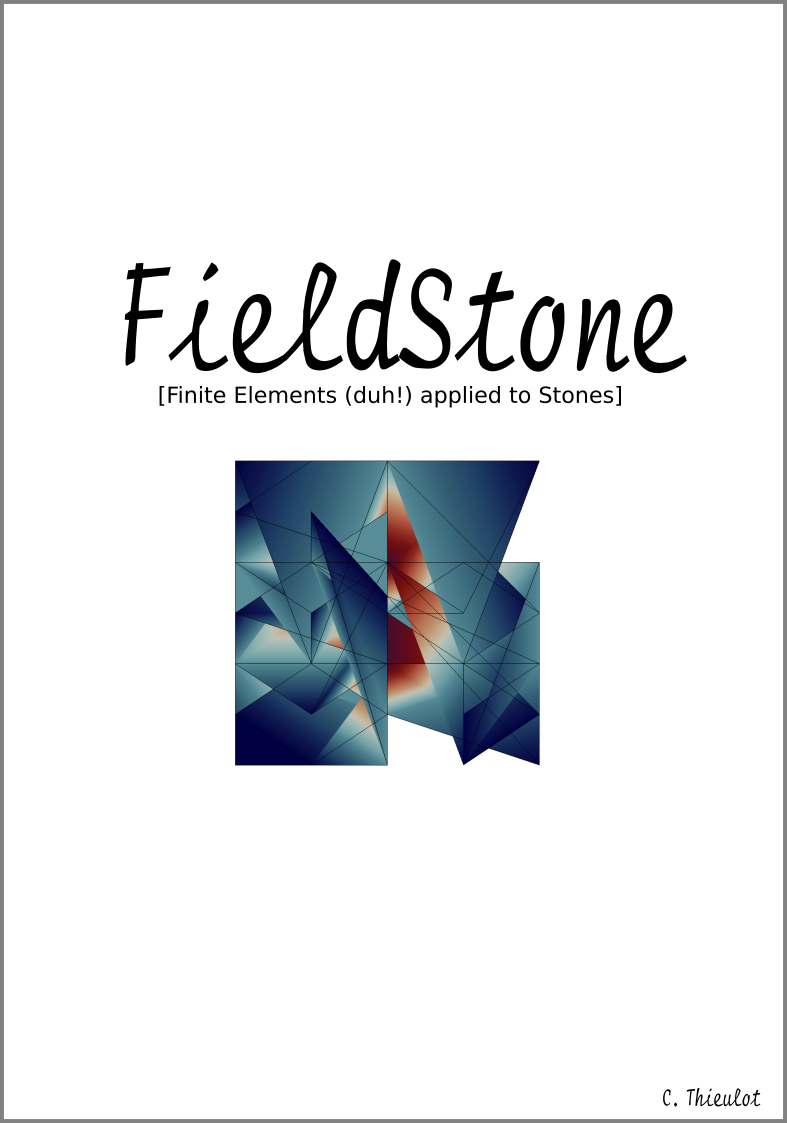
\includegraphics[width=\linewidth]{images/frontpage.png}

With contributions from: Wolfgang Bangerth, Eric van den Hoogen, Job Mos, Lukas van de Wiel. 
\newpage
If you find anything in this document useful for your research please cite it 
as follows ({\it please} include the doi!):
\begin{verbatim}
@article{Thieulot2019,
author = "C.A.P. (Cedric) Thieulot",
title = "{Fieldstone: The Finite Element Method in Computational Geodynamics}",
year = "2019",
month = "8",
url = "https://uu.figshare.com/articles/manual_pdf/9209393",
doi = "10.23644/uu.9209393.v1"
}
\end{verbatim}
\newpage
\maketitle
\tableofcontents
\newpage
\begin{center}
{\color{red} \huge WARNING: this is work in progress}
\end{center}

%%%%%%%%%%%%%%%%%%%%%%%%%%%%%%%%%%%%%%%%%%%%%%%%%%%%%%%%%%%%%%%%%%%%%%%%%%%%%%%
\section{Introduction}

\subsection{Philosophy} 
This document was written with my students in mind, i.e. 3rd and 4th year 
Geology/Geophysics students at Utrecht University. 
I have chosen to use as little jargon as possible unless it is a term that is 
commonly found in the geodynamics literature (methods paper as well as 
application papers). There is no mathematical proof of any theorem that may 
be mentioned but I will try to refer to the appropriate sources, i.e.
generic Numerical Analysic, Finite Element and 
Linear Algebra books. If you find that this books lacks references
to Sobolev spaces, Hilbert spaces, and other spaces, this book is just not for you.  

The codes I provide here are by no means optimised as I have chosen code readability 
over code efficiency. I have also chosen to avoid resorting to multiple code 
files or even functions in order to favour a sequential reading of the codes. 
These codes are not designed to form the basis of a real life application:
Existing open source highly optimised codes shoud be preferred, such as 
ASPECT \cite{krhb12,hedg17}, CITCOM \cite{zhzm00,zhmt08}, LAMEM \cite{kapb16}, 
PTATIN \cite{mabl14,mabl15}, PYLITH \cite{aakw13}, ... (see Appendix~\ref{app:codes}).

All kinds of feedback is welcome on the text (grammar, typos, ...), on the text, the equations
or on the code(s). You will have my eternal gratitude if you wish to contribute an 
example, a benchmark, a cookbook. 

All the python scripts and tex files are freely available at 
\begin{center}
\url{https://github.com/cedrict/fieldstone}
\end{center}
This document is available at:
\begin{center}
\url{http://cedricthieulot.net/manual.pdf}  
\includegraphics[width=0.7cm]{images/minion}
\end{center}

 %-----------------------------------
\subsection{ambition \& motivation} 
I wish to provide the community with:
\begin{itemize}
\item a ginormous bibliography data base - simply search the pdf for keywords. The \LaTeX{} bib
 file\footnote{\url{https://github.com/cedrict/fieldstone/blob/master/biblio_geosciences.bib}} 
is also available next to the manual.tex file on github;  
\item a go-to document for anybody who wants to know more about 
      a particular topic in computational geodynamics;
\item a useful teaching tool for researchers, teachers, students and PhD students alike; 
\item small, readable, educative codes. 
\end{itemize}

 %-----------------------
\subsection{Acknowledgements} 
I have benefitted from many discussions, lectures, tutorials, coffee machine 
discussions, debugging sessions, conference poster sessions, etc ... 
over the years. I wish to name these instrumental people in particular and 
in alphabetic order: 
Wolfgang Bangerth, 
Jean Braun, 
Rens Elbertsen,
Philippe Fullsack, 
Menno Fraters, 
Anne Glerum,
Timo Heister,
Dave May,
Robert Myhill,
John Naliboff,
E. Gerry Puckett,
Melchior Schuh-Senlis,
Michael Tetley,
Lukas van de Wiel,
Arie van den Berg, 
Eric van den Hoogen,
Tom Weir,
and the whole ASPECT family/team. 

%I wish to acknowledge many BSc and MSc students for their questions and feedback.
%and wish to mention: Job Mos (the
%very first version of fieldstone was part of his MSc thesis), 
%Tom Weir (contributions to the compressible formulation - MSc thesis), 
%and Rens Elbertsen (Tosi benchmark - BSc thesis).
 %-----------------------
\subsection{About the author} 
I have BSc in mathematics, and an MSc diploma in physics (with a specialization in 
musical acoustics \cite{dewl02}). I did my PhD at the 
university of Groningen (The Netherlands) titled {\sl Thermodynamically consistent 
fluid particle modelling of phase separating 
mixtures}\footnote{\url{http://cedricthieulot.net/thesis.html}}.
Although half of the thesis deals with the re-derivation of the Navier-Stokes 
equations for such systems\cite{esth03}, the second half is concerned with 
the implementation of these equations with the Smoothed Particle Hydrodynamics
method \cite{thje05a,thje05b,thes05}.

I then taught physics and programming at the University of Rennes (France) for a year, 
after which I did a 2-year post-doc with Prof. J. 
Braun\footnote{\url{https://www.gfz-potsdam.de/en/staff/jean-braun/}} in the 
Geosciences department. 
I then did a 4-year post-doc with prof. R. 
Huismans\footnote{\url{https://folk.uib.no/huismans/}} at the University of Bergen (Norway), 
followed by a 3-year post-doc with profs. T. Torsvik and W. Spakman at the Utrecht
University (The Netherlands). 
Since June 2015 I am assistant professor there in the geophysics group.
 
 %--------------------------------- 
\subsection{Essential/relevant literature} 
\begin{center}
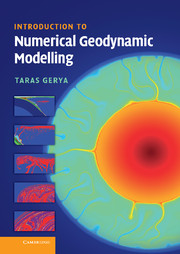
\includegraphics[height=4.5cm]{images/literature/gerya_book}
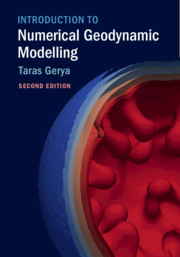
\includegraphics[height=4.5cm]{images/literature/gerya_book2}
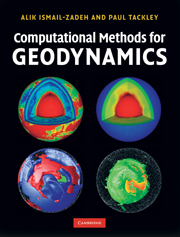
\includegraphics[height=4.5cm]{images/literature/tackley_book}
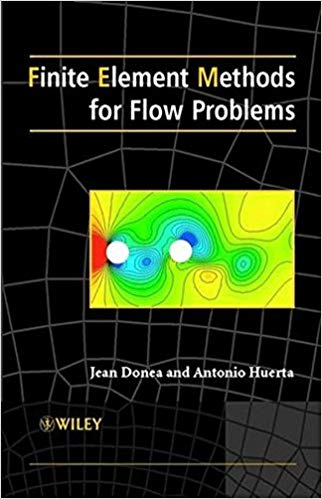
\includegraphics[height=4.5cm]{images/literature/donea_huerta_book}\\
\cite{gery10}     \hspace{1.99cm} 
\cite{gery19book} \hspace{1.99cm} 
\cite{tack10}     \hspace{1.99cm} 
\cite{dohu03}  \\
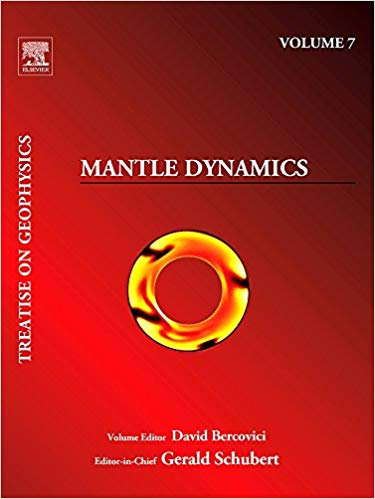
\includegraphics[height=4.5cm]{images/literature/bercovici_book}
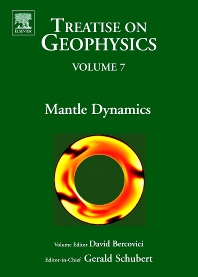
\includegraphics[height=4.5cm]{images/literature/bercovici_book2}
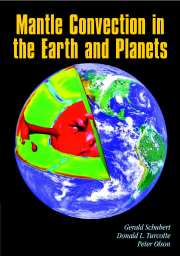
\includegraphics[height=4.5cm]{images/literature/sto_book}
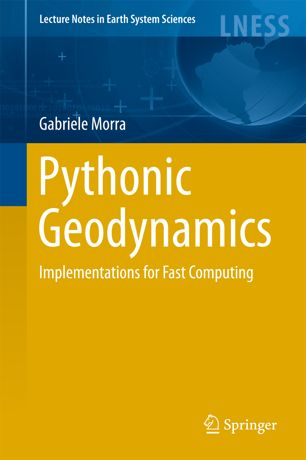
\includegraphics[height=4.5cm]{images/literature/morra_book}\\
\cite{berc09} \hspace{1.99cm} 
\cite{berc15} \hspace{1.99cm} 
\cite{scto01} \hspace{1.99cm} 
\cite{morr18} \\ 
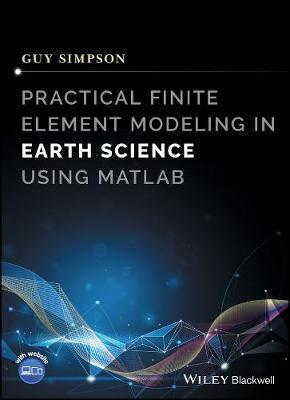
\includegraphics[height=4.5cm]{images/literature/simpson_book}
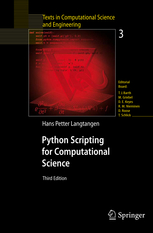
\includegraphics[height=4.5cm]{images/literature/langtangen_book}\\
\cite{simp17} \hspace{1.99cm}
\cite{lang08}
\end{center}

\begin{itemize}
\item {\it Numerical modeling of Earth Systems} by Thorsten W. Becker and Boris J. P. Kaus,\\ 
\url{http://www-udc.ig.utexas.edu/external/becker/teaching-557.html}

\item {\it Myths \& Methods in Modeling} by M. Spiegelman,\\
 \url{https://www.ldeo.columbia.edu/~mspieg/mmm/}

\item {\it Computational Science I} by Matthew G. Knepley,\\
 \url{https://cse.buffalo.edu/~knepley/classes/caam519/Syllabus.html}

\item {\it Introduction to Numerical Methods for Variational Problems} by Hans Petter Langtangen and 
Kent-Andre Mardal, \\
\url{https://hplgit.github.io/fem-book/doc/pub/book/pdf/fem-book-4print.pdf}
\end{itemize}

 %----------------
\subsection{Installation} \begin{flushright} {\tiny {\color{gray} install.tex}} \end{flushright}

%--------------------------------
\subsubsection{Python}

If numpy, scipy or matplotlib are not installed on your machine, here is how you 
can install them:
\begin{verbatim}
sudo apt install python3-numpy
sudo apt install python3-scipy
\end{verbatim}
To install the umfpack solver (check?):
\begin{verbatim}
pip install --upgrade scikit-umfpack --user
\end{verbatim}
If you need to install pip:
\begin{verbatim}
sudo apt install python3-pip
\end{verbatim}

%--------------------------------
\subsubsection{Julia}

In order to have vim supporting the Julia language, do 
\begin{verbatim}
git clone git@github.com:JuliaEditorSupport/julia-vim.git
\end{verbatim}
and copy the content of the julia-vim folder in the .vim folder.
That's it.
 %------------------------------------
\subsection{What is a fieldstone?} \begin{flushright} {\tiny {\color{gray} whatisafieldstone.tex}} \end{flushright}

\begin{center}
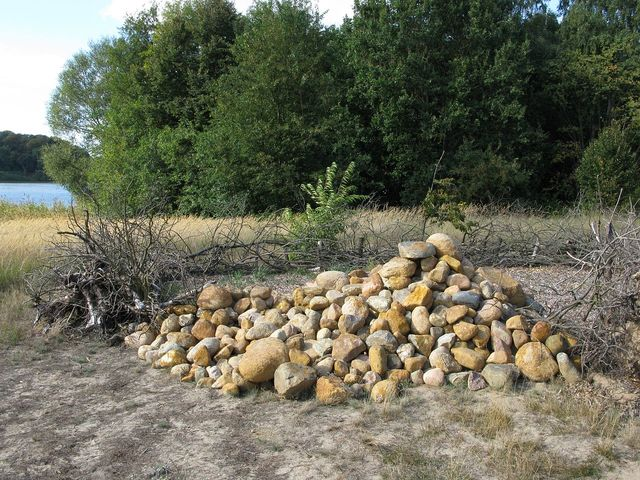
\includegraphics[width=5cm]{images/fieldstone2}\\
{\captionfont Taken from \url{https://en.wikipedia.org/wiki/Fieldstone}}
\end{center}

Simply put, it is a stone collected from the surface of fields where it 
occurs naturally. It also stands for the bad acronym: {\sl fi}nite 
{\sl el}ement {\sl d}eformation of {\sl stone}s which echoes the primary 
application of these codes: geodynamic modelling.
 %-----------------
\subsection{Why the Finite Element method?} \begin{flushright} {\tiny {\color{gray} why.tex}} \end{flushright}

The Finite Element Method (FEM) is by no means the only method 
to solve PDEs in geodynamics, nor it is necessarily always the best one.
Other methods are employed very successfully, such as the Finite Difference 
Method (FDM), the Finite Volume Method (FVM), and to a lesser extent
the Discrete Element Method (DEM) \cite{tasy05,egho07,egsc07,funi14}, 
the Lattice-Boltzmann method \cite{hupc08}, the Rigid Element Method \cite{lacj15},  
or the Element Free Galerkin Method (EFGM) \cite{hans03}.
I have been using FEM since 2008 and I do not have real 
experience to speak of in FVM or FDM (except for chapter 11)
so I concentrate in this book 
on what I know best. 


 %----------------------
\subsection{Notations} Scalars such as temperature, density, pressure, etc ... are simply 
obtained in \LaTeX{} by using the math mode, e.g. $T$, $\rho$, $p$.
Although it is common to lump vectors and matrices/tensors together
by using bold fonts, I have decided in the interest of clarity to 
distinguish between those: vectors are denoted by an arrow 
atop the quantity, e.g. $\vec \upnu$, $\vec g$, while matrices 
and tensors are in bold $\bm M$, $\bm \sigma$, etc ...

Also I use the $\cdot$ notation between two vectors to denote a 
dot product $\vec u \cdot \vec v = u_iv_i$ or a matrix-vector
multiplication ${\bm M}\cdot \vec a = M_{ij}a_j$. If there is no
$\cdot$ between vectors, it means that the result 
$\vec a \vec b = a_ib_j$ is a matrix (it is a dyadic 
product\footnote{\url{https://en.wikipedia.org/wiki/Dyadics}}.
Case in point, $\vec\nabla\cdot\vec\upnu$ is the velocity divergence
while $\vec\nabla\vec\upnu$ is the velocity gradient tensor.
 %-------------------------------------
\subsection{Colour maps for visualisation} In an attempt to homogenise the figures obtained with ParaView, I have decided to use 
a fixed colour scale for each field throughout this document. These colour scales were 
obtained from \url{https://peterkovesi.com/projects/colourmaps} and are 
Perceptually Uniform Colour Maps \cite{kove15}. 

\begin{center}
\begin{tabular}{lll}
\hline
Field & colour code & \\
\hline\hline
Velocity/displacement & CET-D1A & 
\includegraphics[width=3cm]{images/colourscales/CET-D1A}\\
\hline
Pressure& CET-L17 & 
\includegraphics[width=3cm]{images/colourscales/CET-L17}\\
\hline
Velocity divergence& CET-L1 & 
\includegraphics[width=3cm]{images/colourscales/CET-L1}\\
\hline
Density& CET-D3 & 
\includegraphics[width=3cm]{images/colourscales/CET-D3}\\
\hline
Strain rate& CET-R2 & 
\includegraphics[width=3cm]{images/colourscales/CET-R2}\\
\hline
Viscosity & CET-R3 & 
\includegraphics[width=3cm]{images/colourscales/CET-R3}\\
\hline
Temperature & CET-D9 & 
\includegraphics[width=3cm]{images/colourscales/CET-D9}\\
\hline
stress & CET-L18 &  
\includegraphics[width=3cm]{images/colourscales/CET-L18}\\
\hline
Spin tensor & CET-R1 &  
\includegraphics[width=3cm]{images/colourscales/CET-R1}\\
\hline
Composition field & CET-CBD1 &  
\includegraphics[width=3cm]{images/colourscales/CET-CBD1}\\
\hline
\end{tabular}
\end{center}

%https://peterkovesi.com/projects/colourmaps/




 %----------------

%%%%%%%%%%%%%%%%%%%%%%%%%%%%%%%%%%%%%%%%%%%%%%%%%%%%%%%%%%%%%%%%%%%%%%%%%%%%%%%


{\small 

\noindent stone 01: simple analytical solution: "Donea \& Huerta" mms \ref{mms1} 
\lstinputlisting[language=bash,basicstyle=\tiny]{python_codes/fieldstone_01/keywords}

\noindent stone 02: Stokes sphere in 2D 
\lstinputlisting[language=bash,basicstyle=\tiny]{python_codes/fieldstone_02/keywords}

\noindent stone 03: Convection in a 2D box: "Blankenbach" benchmark \cite{blbc89}
\lstinputlisting[language=bash,basicstyle=\tiny]{python_codes/fieldstone_03/keywords}

\noindent stone 04: The lid driven cavity
\lstinputlisting[language=bash,basicstyle=\tiny]{python_codes/fieldstone_04/keywords}

\noindent stone 05: SolCx
\lstinputlisting[language=bash,basicstyle=\tiny]{python_codes/fieldstone_05/keywords}

\noindent stone 06: SolKz
\lstinputlisting[language=bash,basicstyle=\tiny]{python_codes/fieldstone_06/keywords}

\noindent stone 07: SolKz
\lstinputlisting[language=bash,basicstyle=\tiny]{python_codes/fieldstone_07/keywords}

\noindent stone 08: The indentor (punch problem) 
\lstinputlisting[language=bash,basicstyle=\tiny]{python_codes/fieldstone_08/keywords}

\noindent stone 09: the annulus benchmark 
\lstinputlisting[language=bash,basicstyle=\tiny]{python_codes/fieldstone_09/keywords}

\noindent stone 10: Stokes sphere (3D) - penalty
\lstinputlisting[language=bash,basicstyle=\tiny]{python_codes/fieldstone_10/keywords}

\noindent stone 11: Stokes sphere (3D) - mixed formulation
\lstinputlisting[language=bash,basicstyle=\tiny]{python_codes/fieldstone_11/keywords}

\noindent stone 12: consistent pressure recovery 
\lstinputlisting[language=bash,basicstyle=\tiny]{python_codes/fieldstone_12/keywords}

\noindent stone 13: the Particle in Cell technique (1) - the effect of averaging
\lstinputlisting[language=bash,basicstyle=\tiny]{python_codes/fieldstone_13/keywords}

\noindent stone 14: solving the full saddle point problem with $Q_1\times P_0$ elements 
\lstinputlisting[language=bash,basicstyle=\tiny]{python_codes/fieldstone_14/keywords}

\noindent stone 16: saddle point problem with Schur complement approach - Stokes sphere 
\lstinputlisting[language=bash,basicstyle=\tiny]{python_codes/fieldstone_16/keywords}

\noindent stone 17: Solving the full saddle point problem in 3D - Burstedde benchmark \cite{dobo04} 
\lstinputlisting[language=bash,basicstyle=\tiny]{python_codes/fieldstone_17/keywords}

\noindent stone 18: Solving the full saddle point problem with $Q_2\times Q_1$ elements 
\lstinputlisting[language=bash,basicstyle=\tiny]{python_codes/fieldstone_18/keywords}

\noindent stone 19: Solving the full saddle point problem with $Q_3\times Q_2$ elements 
\lstinputlisting[language=bash,basicstyle=\tiny]{python_codes/fieldstone_19/keywords}

\noindent stone 20: Convection in a 3D box, the Busse benchmark \cite{bucc93}
\lstinputlisting[language=bash,basicstyle=\tiny]{python_codes/fieldstone_20/keywords}

\noindent stone 22: The stabilised $Q_1 \times Q_1$ element 
\lstinputlisting[language=bash,basicstyle=\tiny]{python_codes/fieldstone_22/keywords}

\noindent stone 23: compressible flow (1) - analytical benchmark 
\lstinputlisting[language=bash,basicstyle=\tiny]{python_codes/fieldstone_23/keywords}


\noindent stone 25: Rayleigh-Taylor instability (1) - instantaneous \cite{vaks97}
\lstinputlisting[language=bash,basicstyle=\tiny]{python_codes/fieldstone_25/keywords}

\noindent stone 28: convection 2D box - Tosi et al, 2015
\lstinputlisting[language=bash,basicstyle=\tiny]{python_codes/fieldstone_28/keywords}

\noindent stone 30: the Particle in Cell technique (2) - CVI algorithms
\lstinputlisting[language=bash,basicstyle=\tiny]{python_codes/fieldstone_30/keywords}

\noindent stone 33: Convection in an annulus 
\lstinputlisting[language=bash,basicstyle=\tiny]{python_codes/fieldstone_33/keywords}

\noindent stone 39: Choi \& Pedersen visco-plasticity benchmarks 
\lstinputlisting[language=bash,basicstyle=\tiny]{python_codes/fieldstone_39/keywords}

\noindent stone 40: Rayleigh-Taylor instability (instantaneous)
\lstinputlisting[language=bash,basicstyle=\tiny]{python_codes/fieldstone_40/keywords}

\noindent stone 44: Flat slab setup 
\lstinputlisting[language=bash,basicstyle=\tiny]{python_codes/fieldstone_44/keywords}

\noindent stone 46: MMS1 with Crouzeix-Raviart ($P_2^+\times P_{-1}$) elements  
\lstinputlisting[language=bash,basicstyle=\tiny]{python_codes/fieldstone_46/keywords}

\noindent stone 47: MMS1 with MINI ($P_1^+\times P_1$) elements
\lstinputlisting[language=bash,basicstyle=\tiny]{python_codes/fieldstone_47/keywords}

\noindent stone 48: $Q_1\times P_0$, $Q_2\times Q_1$, $Q_3\times Q_2$ and $Q_4\times Q_3$ elements
\lstinputlisting[language=bash,basicstyle=\tiny]{python_codes/fieldstone_48/keywords}

\noindent stone 49: Consistent Boundary Flux method on D\&H benchmark with 4 elements 
\lstinputlisting[language=bash,basicstyle=\tiny]{python_codes/fieldstone_49/keywords}

\noindent stone 50: Lithosphere extension (visco-plastic, thermo-mechanically coupled)
\lstinputlisting[language=bash,basicstyle=\tiny]{python_codes/fieldstone_50/keywords}

\noindent stone 51: Triangular domain benchmark with MINI element
\lstinputlisting[language=bash,basicstyle=\tiny]{python_codes/fieldstone_51/keywords}

\noindent stone 52: Serendipity element in 2D 
\lstinputlisting[language=bash,basicstyle=\tiny]{python_codes/fieldstone_52/keywords}

\noindent stone 53: the sinking block benchmark  
\lstinputlisting[language=bash,basicstyle=\tiny]{python_codes/fieldstone_53/keywords}

\noindent stone 54: free surface and ALE algorithms
\lstinputlisting[language=bash,basicstyle=\tiny]{python_codes/fieldstone_54/keywords}

\noindent stone 55: Subduction as a thin-sheet problem
\lstinputlisting[language=bash,basicstyle=\tiny]{python_codes/fieldstone_55/keywords}

\noindent stone 57: 1D steady state diffusion with DG-FEM
\lstinputlisting[language=bash,basicstyle=\tiny]{python_codes/fieldstone_57/keywords}

\noindent stone 58: Elastic disk under compression
\lstinputlisting[language=bash,basicstyle=\tiny]{python_codes/fieldstone_58/keywords}

\noindent stone 59: Ice flow down an inclined plane 
\lstinputlisting[language=bash,basicstyle=\tiny]{python_codes/fieldstone_59/keywords}

\noindent stone 60: 1D advection with DG-FEM 
\lstinputlisting[language=bash,basicstyle=\tiny]{python_codes/fieldstone_60/keywords}

\noindent stone 63: Failure in cemented granular material
\lstinputlisting[language=bash,basicstyle=\tiny]{python_codes/fieldstone_63/keywords}

\noindent stone 67: Newtonian subduction setups \& Particle-in-cell
\lstinputlisting[language=bash,basicstyle=\tiny]{python_codes/fieldstone_67/keywords}

\noindent stone 68: subduction \& corner flow
\lstinputlisting[language=bash,basicstyle=\tiny]{python_codes/fieldstone_68/keywords}

\noindent stone 69: Spherical shell 
\lstinputlisting[language=bash,basicstyle=\tiny]{python_codes/fieldstone_69/keywords}

}









 %%%%%%%%%%%%%%%%%%%%%%%%%%%%%%%%%%%%%%%%%%%%%%%%%%%%%%%%%%%%%%%%%%
%%%%%%%%%%%%%%%%%%%%%%%%%%%%%%%%%%%%%%%%%%%%%%%%%%%%%%%%%%%%%%%%%%%%%%%%%%%%%%%

\newpage
%%%%%%%%%%%%%%%%%%%%%%%%%%%%%%%%%%%%%%%%%%%%%%%%%%%%%%%%%%%%%%%%%%%%%%%%%%%%%%%
\section{The physical equations} %%%%%%%%%%%%%%%%%%%%%%%%%%%%%%%%%%%%%%%%%%%%%%

\begin{center}
\begin{tabular}{lll}
\hline
Symbol & meaning & unit \\
\hline
\hline
$t$ & Time & s \\
$x,y,z$ & Cartesian coordinates & m \\
${\bm v}$ & velocity vector & m$\cdot$ s$^{-1}$\\
$\rho$ & mass density & kg/m$^3$ \\
$\eta$ & dynamic viscosity &  Pa$\cdot$ s \\
$\lambda$ & penalty parameter & Pa$\cdot$ s \\
$T$ & temperature & K \\
${\bm \nabla}$ & gradient operator & m$^{-1}$ \\
${\bm \nabla}\cdot$ & divergence operator & m$^{-1}$ \\
$p$ & pressure & Pa\\
$\dot{\bm \varepsilon}({\bm v})$ & strain rate tensor & s$^{-1}$ \\
$\alpha$ & thermal expansion coefficient & K$^{-1}$ \\
$k$ & thermal conductivity & W/(m $\cdot$ K) \\
$C_p$ & Heat capacity & J/K \\
$H$ & intrinsic specific heat production & W/kg\\
$\beta_T$ & isothermal compressibility & Pa$^{-1}$  \\
${\bm \tau}$ & deviatoric stress tensor & Pa \\
${\bm \sigma}$ & full stress tensor & Pa \\
\hline
\end{tabular}
\end{center}

%------------------------------------------------------------------------
\subsection{The heat transport equation - energy conservation equation}

Let us start from the heat transport equation as shown in Schubert, Turcotte and Olson \cite{scto01}:
\[
\rho C_p \frac{DT}{Dt} - \alpha T \frac{Dp}{Dt} = {\bm \nabla} \cdot k {\bm \nabla} T + \Phi + \rho H  
\]
with $D/Dt$ being the total derivatives so that 
\[
\frac{DT}{Dt} = \frac{\partial T}{\partial t} + {\bm v}\cdot {\bm \nabla}T
\quad\quad
\frac{Dp}{Dt} = \frac{\partial p}{\partial t} + {\bm v}\cdot {\bm \nabla}p
\]
Solving for temperature, this equation is often rewritten as follows:
\begin{mdframed}[backgroundcolor=blue!5]
\[
\rho C_p \frac{DT}{Dt} - {\bm \nabla} \cdot k {\bm \nabla} T =  \alpha T \frac{Dp}{Dt} + \Phi + \rho H  
\]
\end{mdframed}

A note on the shear heating term $\Phi$: In many publications, $\Phi$ 
is given by $\Phi=\tau_{ij}\partial_j u_i={\bm \tau}:{\bm \nabla}{\bm v}$.

\begin{eqnarray}
\Phi 
&=& \tau_{ij}\partial_j u_i \nonumber\\
&=& 2 \eta \dot{\varepsilon}_{ij}^d\partial_j u_i \nonumber\\
&=& 2 \eta \frac{1}{2}\left( \dot{\varepsilon}_{ij}^d\partial_j u_i + \dot{\varepsilon}_{ji}^d\partial_i u_j \right) \nonumber\\
&=& 2 \eta \frac{1}{2}\left( \dot{\varepsilon}_{ij}^d\partial_j u_i + \dot{\varepsilon}_{ij}^d\partial_i u_j \right) \nonumber\\
&=& 2 \eta  \dot{\varepsilon}_{ij}^d  \frac{1}{2}\left(\partial_j u_i + \partial_i u_j \right) \nonumber\\
&=& 2 \eta  \dot{\varepsilon}_{ij}^d   \dot{\varepsilon}_{ij} \nonumber\\
&=& 2 \eta  \dot{\bm \varepsilon}^d :  \dot{\bm \varepsilon} \nonumber\\
&=& 2 \eta  \dot{\bm \varepsilon}^d : \left( \dot{\bm \varepsilon}^d +\frac{1}{3} ({\bm \nabla}\cdot{\bm v}) {\bm 1} \right)\nonumber\\
&=& 2 \eta  \dot{\bm \varepsilon}^d : \dot{\bm \varepsilon}^d 
+ 2 \eta  \dot{\bm \varepsilon}^d : {\bm 1} ({\bm \nabla}\cdot{\bm v}) \nonumber\\ 
&=& 2 \eta  \dot{\bm \varepsilon}^d : \dot{\bm \varepsilon}^d 
\end{eqnarray}
Finally
\[
\Phi = {\bm \tau}:{\bm \nabla}{\bm v} = 2 \eta  \dot{\bm \varepsilon}^d : \dot{\bm \varepsilon}^d
= 2 \eta \left( (\dot{\varepsilon}_{xx}^d)^2 + (\dot{\varepsilon}_{yy}^d)^2 + 2(\dot{\varepsilon}_{xy}^d)^2 \right)
\]

%------------------------------------------------------------------------
\subsection{The momentum conservation equations} 

Because the Prandlt number is virtually zero in Earth science applications the Navier Stokes 
equations reduce to the Stokes equation:
\[
{\bm \nabla}\cdot {\bm \sigma} + \rho {\bm g} = 0
\]
Since 
\[
{\bm \sigma} = -p {\bm 1} + {\bm \tau}
\]
it also writes
\[
-{\bm \nabla}p + {\bm \nabla}\cdot {\bm \tau} + \rho {\bm g} = 0
\]
Using the relationship ${\bm \tau} = 2 \eta \dot{\bm \varepsilon}^d$ we arrive at 
\begin{mdframed}[backgroundcolor=blue!5]
\[
-{\bm \nabla}p + {\bm \nabla}\cdot (2 \eta \dot{\bm \varepsilon}^d ) + \rho {\bm g} = 0
\]
\end{mdframed}

%------------------------------------------------------------------------
\subsection{The mass conservation equations} 

The mass conservation equation is given by
\[
\frac{D\rho}{Dt} + \rho {\bm \nabla}\cdot{\bm v} = 0
\]
or, 
\begin{mdframed}[backgroundcolor=blue!5]
\[
\frac{\partial \rho}{\partial t} + {\bm \nabla}\cdot(\rho {\bm v}) = 0
\]
\end{mdframed}
In the case of an incompressible flow, then $\partial \rho/\partial t=0$ and 
${\bm \nabla}\rho=0$, i.e. $D\rho/Dt=0$ and the remaining equation is simply:
\[
{\bm \nabla}\cdot{\bm v} = 0
\]

\subsection{The equations in ASPECT manual}
The following is lifted off the ASPECT manual.
We focus on the system of equations in a $d=2$- or $d=3$-dimensional
domain $\Omega$ that describes the motion of a highly viscous fluid driven
by differences in the gravitational force due to a density that depends on
the temperature. In the following, we largely follow the exposition of this
material in Schubert, Turcotte and Olson \cite{scto01}.

Specifically, we consider the following set of equations for velocity $\mathbf
u$, pressure $p$ and temperature $T$:
\begin{align}
  \label{eq:stokes-1}
  -\nabla \cdot \left[2\eta \left(\dot\varepsilon(\bm v)
                                  - \frac{1}{3}(\nabla \cdot \bm v)\mathbf 1\right)
                \right] + \nabla p &=
  \rho \bm g
  &
  & \textrm{in $\Omega$},
  \\
  \label{eq:stokes-2}
  \nabla \cdot (\rho \bm v) &= 0
  &
  & \textrm{in $\Omega$},
  \\
  \label{eq:temperature}
  \rho C_p \left(\frac{\partial T}{\partial t} + \bm v\cdot\nabla T\right)
  - \nabla\cdot k\nabla T
  &=
  \rho H
  \notag
  \\
  &\quad
  +
  2\eta
  \left(\dot\varepsilon(\bm v) - \frac{1}{3}(\nabla \cdot \bm v)\mathbf 1\right)
  :
  \left(\dot\varepsilon(\bm v) - \frac{1}{3}(\nabla \cdot \bm v)\mathbf 1\right)
  \\
  &\quad
  +\alpha T \left( \bm v \cdot \nabla p \right)
  \notag
  \\
  &\quad
  &
  & \textrm{in $\Omega$},
  \notag
\end{align}
where $\dot{\bm \varepsilon}(\mathbf u) = \frac{1}{2}(\nabla \mathbf u + \nabla\mathbf
u^T)$ is the symmetric gradient of the velocity (often called the
\textit{strain rate}).%

In this set of equations, \eqref{eq:stokes-1} and \eqref{eq:stokes-2}
represent the compressible Stokes equations in which $\mathbf v=\mathbf
v(\mathbf x,t)$ is the velocity field and $p=p(\mathbf x,t)$ the pressure
field. Both fields depend on space $\mathbf x$ and time $t$. Fluid flow is
driven by the gravity force that acts on the fluid and that is proportional to
both the density of the fluid and the strength of the gravitational pull.

Coupled to this Stokes system is equation \eqref{eq:temperature} for the
temperature field $T=T(\mathbf x,t)$ that contains heat conduction terms as
well as advection with the flow velocity $\mathbf v$. The right hand side
terms of this equation correspond to
\begin{itemize}
\item internal heat production for example due to radioactive decay;
\item friction (shear) heating;
\item adiabatic compression of material;
\end{itemize}

In order to arrive at the set of equations that ASPECT solves, 
we need to 
\begin{itemize}
\item neglect the $\partial p/\partial t$. {\color{red}WHY?}
\item neglect the $\partial \rho / \partial t$ . {\color{red}WHY?}
\end{itemize}
from equations above. 

----------------------------------------

Also, their definition of the shear heating term $\Phi$ is:
\[
\Phi = k_B ({\bm \nabla}\cdot{\bm v})^2 + 2\eta \dot{\bm \varepsilon}^d:\dot{\bm \varepsilon}^d
\]
For many fluids the bulk viscosity $k_B$ is very small and is often taken to be zero, an assumption known
as the Stokes assumption: $k_B=\lambda+2\eta/3=0$. \index{bulk viscosity}
Note that $\eta$ is the dynamic viscosity and $\lambda$ the second viscosity. \index{dynamic viscosity}
\index{second viscosity}
Also, 
\[
{\bm \tau}=2\eta \dot{\bm \varepsilon} + \lambda ({\bm \nabla}\cdot{\bm v}) {\bm 1}
\]
but since $k_B=\lambda+2\eta/3=0$, then $\lambda=-2\eta/3$ so 
\[
{\bm \tau}=2\eta \dot{\bm \varepsilon} -\frac{2}{3}\eta ({\bm \nabla}\cdot{\bm v}) {\bm 1} = 2\eta \dot{\bm \varepsilon}^d
\]







\newpage
%---------------------------------
\subsection{the Boussinesq approximation: an Incompressible flow}

\index{Boussinesq}

[from aspect manual]
The Boussinesq approximation assumes that the density can be
considered constant in all occurrences in the equations with the exception of
the buoyancy term on the right hand side of \eqref{eq:stokes-1}. The primary
result of this assumption is that the continuity equation \eqref{eq:stokes-2}
will now read
\[
{\bm \nabla}\cdot{\bm v} = 0
\]
This implies that the strain rate tensor is deviatoric.
Under the Boussinesq approximation, the equations are much simplified:

\begin{align}
  \label{eq:stokes-1}
  -\nabla \cdot \left[2\eta \dot{\bm \varepsilon}(\bm v)
                \right] + \nabla p &=
  \rho \bm g
  &
  & \textrm{in $\Omega$},
  \\
  \label{eq:stokes-2}
  \nabla \cdot (\rho \bm v) &= 0
  &
  & \textrm{in $\Omega$},
  \\
  \label{eq:temperature}
  \rho_0 C_p \left(\frac{\partial T}{\partial t} + \bm v\cdot\nabla T\right)
  - \nabla\cdot k\nabla T
  &=
  \rho H
  &
  & \textrm{in $\Omega$}
\end{align}
Note that all terms on the rhs of the temperature equations have disappeared, with the exception 
of the source term.


\newpage
%%%%%%%%%%%%%%%%%%%%%%%%%%%%%%%%%%%%%%%%%%%%%%%%%%%%%%%%%%%%%%%%%%%%%%%%%%%%%%%%%%%%%%%%%%55
\subsection{Stokes equation for elastic medium}

What follows is mostly borrowed from Becker \& Kaus lecture notes.

%\begin{tabular}{|l|l|l|}
%\hline
%${\bm u}       $ & displacement vector &   \\
%${\bm \sigma}  $ & full stress tensor  & Pa\\
%${\bm \epsilon}$ & strain tensor       &   \\
%${\bm 1}       $ & unit tensor         &   \\
%${\bm f}       $ & body forces         &   \\
%\hline
%\end{tabular}

The strong form of the PDE that governs force balance in a medium is given by
\[
{\bm \nabla}\cdot{\bm \sigma}  + {\bm f} = {\bm 0}
\]
where ${\bm \sigma}$ is the stress tensor and ${\bm f}$ is a body force.

The stress tensor is related to the strain tensor through the generalised 
Hooke's law:
\begin{equation}
\sigma_{ij}=\sum_{kl}C_{ijkl}\epsilon{kl} \label{eq:one}
\end{equation}
where ${\bm C}$ is the fourth-order elastic tensor.
In the case of an isotropic material, this relationship simplifies to
\begin{equation}
\sigma_{ij}=\lambda \epsilon_{kk} \delta_{ij} + 2\mu \epsilon_{ij}
\quad\quad
or, 
\quad\quad
{\bm \sigma} = \lambda ({\bm \nabla}\cdot{\bm u})  {\bm 1} + 2\mu {\bm \epsilon}   \label{eq:two}
\end{equation}
where $\lambda$ is the Lam\'e parameter and $\mu$ is the shear modulus\footnote{It is also sometimes written $G$}.
The term ${\bm \nabla}\cdot{\bm u}$ is the isotropic dilation.

\index{Lam\'e parameter} \index{shear modulus}

The strain tensor is related to the displacement as follows: \index{strain tensor}
\[
{\bm \epsilon} = \frac{1}{2}({\bm \nabla}{\bm u} + {\bm \nabla}{\bm u}^T)
\]

The incompressibility (bulk modulus), $K$, is defined as $p=-K {\bm \nabla}\cdot{\bm u}$ 
where $p$ is the pressure with \index{bulk modulus}
\begin{eqnarray}
p&=&-\frac{1}{3}Tr({\bm \sigma}) \nonumber\\
 &=& -\frac{1}{3} [ \lambda ({\bm \nabla}\cdot{\bm u}) Tr[{\bm 1}] + 2 \mu Tr[{\bm \epsilon}]] \nonumber\\
 &=& -\frac{1}{3} [ \lambda ({\bm \nabla}\cdot{\bm u})  3  + 2 \mu  ({\bm \nabla}\cdot{\bm u}) ] \nonumber\\
 &=& -[ \lambda  + \frac{2}{3} \mu ]   ({\bm \nabla}\cdot{\bm u})  
\end{eqnarray}
so that $K=\lambda+\frac{2}{3}\mu$.

%or
%\[
%\mu=\frac{3K(1-2\nu)}{2(1+\nu)}
%\]


\paragraph{Remark}: Eq. (\ref{eq:one}) and (\ref{eq:two}) are analogous to the ones that one has to solve
in the context of viscous flow using the penalty method. In this case $\lambda$ is the penalty coefficient, 
${\bm u}$ is the velocity, and $\mu$ is then the dynamic viscosity.

%\begin{center}
%\includegraphics[width=15cm]{images/coeffs}\\
%{\small Homogeneous isotropic linear elastic materials have their elastic properties uniquely determined by any two moduli among these; thus, given any two, any other of the elastic moduli can be calculated according to these formulas.}
%\end{center}

The Lam\'e parameter and the shear modulus are also linked to $\nu$ the poisson ratio, 
and $E$, Young's modulus: \index{Poisson ratio} \index{Young's modulus}
\[
\lambda=\mu\frac{2\nu}{1-2\nu}
=\frac{\nu E}{(1+\nu)(1-2\nu)}
\quad\quad
{\rm with}
\quad\quad
E=2\mu(1+\nu)
\]
The shear modulus, expressed often in GPa, describes the material's response to shear stress.
The poisson ratio describes the response in the direction orthogonal to uniaxial stress.
The Young modulus, expressed in GPa, describes the material's strain response to uniaxial stress in the 
direction of this stress.


%%%%%%%%%%%%%%%%%%%%%%%%%%%%%%%%%%%%%%%%%%%%%%%%%%%%%%%%%%%%%%%%%%55
\newpage
\subsection{The strain rate tensor in all coordinate systems}

The strain rate tensor $\dot{\bm\varepsilon}$ is given by
\begin{equation}
\dot{\bm \varepsilon} = \frac{1}{2}( {\bm \nabla}{\bm v}+ {\bm \nabla}{\bm v}^T) 
\end{equation}

\subsubsection{Cartesian coordinates}
\begin{eqnarray}
\dot\varepsilon_{xx} &=& \frac{\partial u}{\partial x} \\
\dot\varepsilon_{yy} &=& \frac{\partial v}{\partial y} \\
\dot\varepsilon_{zz} &=& \frac{\partial w}{\partial z} \\
\dot\varepsilon_{yx} =
\dot\varepsilon_{xy} &=& \frac{1}{2} \left( \frac{\partial u}{\partial y} + \frac{\partial v}{\partial x}  \right)\\
\dot\varepsilon_{zx} =
\dot\varepsilon_{xz} &=& \frac{1}{2} \left( \frac{\partial u}{\partial z} + \frac{\partial w}{\partial x}  \right)\\
\dot\varepsilon_{zy} =
\dot\varepsilon_{yz} &=& \frac{1}{2} \left( \frac{\partial v}{\partial z} + \frac{\partial w}{\partial y}  \right)
\end{eqnarray}

\subsubsection{Polar coordinates}

\begin{eqnarray}
\dot\varepsilon_{rr} &=& \frac{\partial v_r}{\partial r} \\
\dot\varepsilon_{\theta\theta} &=& \frac{v_r}{r} + \frac{1}{r} \frac{\partial v_\theta}{\partial \theta}  \\
\dot\varepsilon_{\theta r} =
\dot\varepsilon_{r\theta} &=& \frac{1}{2} \left(   \frac{\partial v_\theta}{\partial r} - \frac{v_\theta}{r} 
+\frac{1}{r} \frac{\partial v_r}{\partial \theta}  \right) 
\end{eqnarray}

\subsubsection{Cylindrical coordinates}

http://eml.ou.edu/equation/FLUIDS/STRAIN/STRAIN.HTM

\subsubsection{Sperical coordinates}

\begin{eqnarray}
\dot\varepsilon_{rr} &=& \frac{\partial v_r}{\partial r} \\
\dot\varepsilon_{\theta\theta} &=& \frac{v_r}{r} + \frac{1}{r} \frac{\partial v_\theta}{\partial \theta}  \\
\dot\varepsilon_{\phi\phi} &=& \frac{1}{r \sin\theta} \frac{\partial v_\phi}{\partial \phi} \\
\dot\varepsilon_{\theta r} =
\dot\varepsilon_{r\theta}   &=& \frac{1}{2} \left( r \frac{\partial}{\partial r} (\frac{v_\theta}{r} ) 
+\frac{1}{r} \frac{\partial v_r}{\partial \theta} \right) \\
\dot\varepsilon_{\phi r} =
\dot\varepsilon_{r\phi}      &=&  \frac{1}{2} \left(  \frac{1}{r \sin\theta} \frac{\partial v_r}{\partial \phi} 
+ r \frac{\partial }{\partial r} (\frac{v_\phi}{r}) \right)  \\
\dot\varepsilon_{\phi \theta} =
\dot\varepsilon_{\theta\phi} &=& \frac{1}{2} \left( \frac{\sin \theta}{r} \frac{\partial }{\partial \theta} (\frac{v_\phi}{\sin\theta}) + \frac{1}{r \sin\theta} \frac{\partial v_\theta}{\partial \phi}    \right) 
\end{eqnarray}






 %%%%%%%%%%%%%%%%%%%%%%%%%%%%%%%%%%%%%%%%%%%%%%%%%%%%%%%%%%%%%%%
\subsection{Rheology in geodynamics} \begin{flushright} {\tiny {\color{gray} rheology.tex}} \end{flushright}

The reader is referred to Barnes \cite{barn99}
for a discussion and review of non-linear viscous rheologies and 
to Coussot \cite{cous14} for a review of experimental data for yield stress fluid
flows. See also Tanner \& Tanner \cite{tata03} for a summary of Heinrich Hencky's 
scientific work on rheology. 

Here is a quick recap of notations:

\begin{center}
\begin{tabular}{ll}
\hline
${\bm \sigma}$ & (full) stress tensor \\
$\sigma_1$, $\sigma_2$, $\sigma_3$ & principal stresses \\ 
${\bm \tau}$   & deviatoric stress tensor \\
$\tau_1$, $\tau_2$, $\tau_3$ & principal deviatoric stresses \\ 
${\cal I}_1({\bm T})$ & first moment invariant of tensor ${\bm T}$ \\
${\cal I}_2({\bm T})$ & second moment invariant of tensor ${\bm T}$ \\
${\cal I}_3({\bm T})$ & third moment invariant of tensor ${\bm T}$ \\
${\tau}_{e}=\sqrt{{\cal I}_2({\bm \tau})}$ & effective deviatoric stress \\
$\dot{{\varepsilon}}_{e}=\sqrt{{\cal I}_2(\dot{\bm \varepsilon}^d)}$ & effective deviatoric strain rate \\
\hline
\end{tabular}
\end{center}

The Cauchy stress tensor is given by 
${\bm \sigma}=-p {\bm 1} + {\bm \tau}$ so that 
${\cal I}_1({\bm \sigma})=-p {\cal I}_1({\bm 1}) + {\cal I}_1({\bm \tau})$.
Since ${\bm \tau}$ is deviatoric, its first invariant is zero. We then have
${\cal I}_1({\bm \sigma})=-p\;  n_D$ where $n_D$ is the number of dimensions.

%.....................................................................
\subsubsection{Linear viscous aka Newtonian} \index{general}{Newtonian fluid}

Simply put, a Newtonian fluid is a fluid in which the viscous stresses at 
every point are linearly proportional 
to the local strain rate.
Mathematically speaking, this means that the fourth-order tensor ${\bm C}$ relating the viscous stress 
tensor to the strain rate tensor does not depend on the stress state and velocity of the flow.
\begin{equation}
{\bm \tau}={\bm C} : \dot{\bm \varepsilon}
\end{equation}
One very often makes the assumption that the fluid is isotropic, i.e. its mechanical properties are the 
same along any direction. As a consequence the fourth order viscosity tensor 
${\bm C}$ is symmetric and will have only two independent real parameters: 
a bulk viscosity coefficient, that defines the resistance of the medium to gradual uniform compression; 
and a dynamic viscosity coefficient $\eta$ that expresses its resistance to gradual 
shearing\footnote{We here neglect the so-called rotational viscosity coefficient which results 
from a coupling between the fluid flow and the rotation of the individual particles}.

Rather logically we denote by non-Newtonian fluids which are not Newtonian, i.e. their viscosity (tensor)
depends on stress. Such fluids are part of our daily life, e.g. honey, toothpaste, paint, blood, or shampoo.
They are also sometimes denoted as Generalized Newtonian Fluid \index{general}{Generalized Newtonian Fluid}. 

\begin{center}
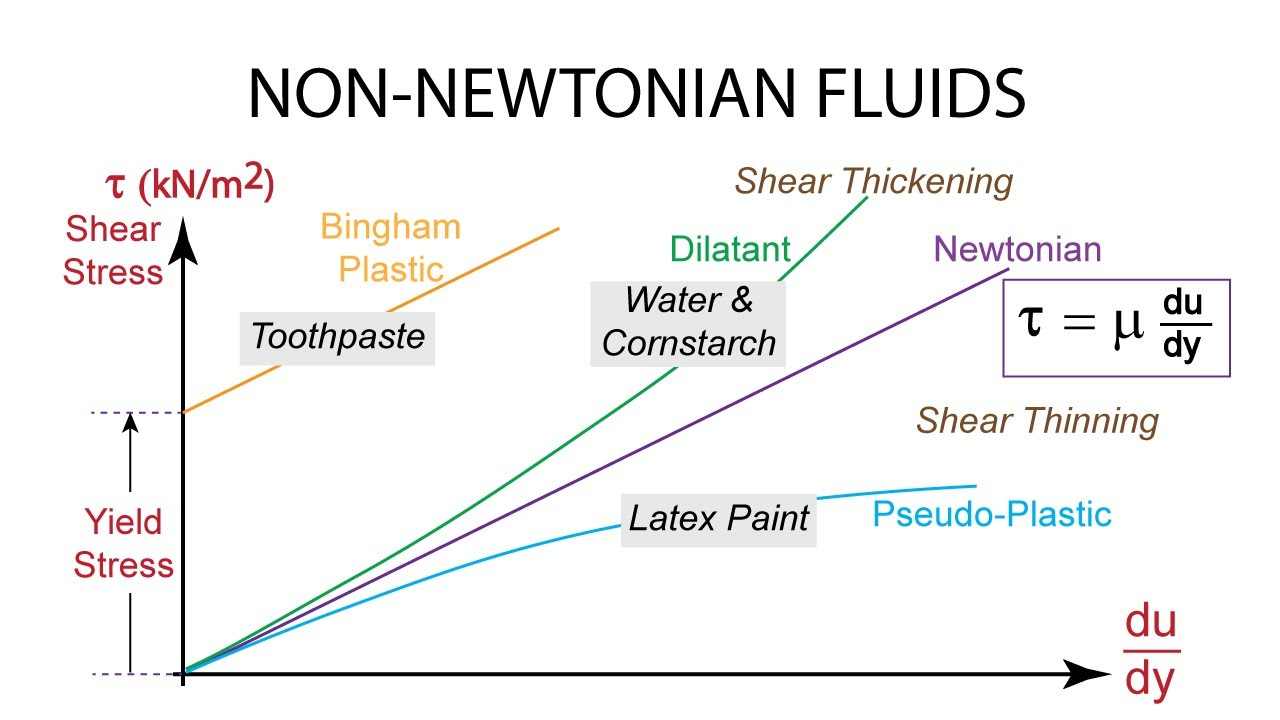
\includegraphics[width=7cm]{images/rheology/nnf}\\
{\captionfont no idea where this comes from ...}
\end{center}

%.....................................................................
\subsubsection{Power-law model \label{ss:powerlaw}} \index{general}{Power Law Rheology}

One of the simplest non-Newtonian viscosity model is the power law model, 
for which the viscosity depends on the (effective) deviatoric strain rate as follows:
\begin{equation}
\eta(\dot{\varepsilon}_e) = K \dot{\varepsilon}_{e}^{n-1}
\qquad \text{or } \qquad
\sigma = 2 K \dot{\varepsilon}_e ^n 
\end{equation}
where $n$ and $K$ are parameters. $n$ is called the power law index. $\dot{\varepsilon}_e$ 
is defined in  \eqref{eq:tauepse} and in the table here above. 
Note that a Newtonian viscosity is recovered when $n=1$. Also $n$ and $K$ may depend on temperature
(see Reddy  \cite[p339]{reddybook2}).

A so-called 'generalised' power law rheology is proposed in Iaffaldano \& bunge (2009) \cite{iabu09}:
\begin{equation}
\eta = K (\dot{\varepsilon}_{e}+\dot{\varepsilon}_0)^{n-1}
\end{equation}
so that in the rigid areas where $\dot{\varepsilon}_e \rightarrow 0$ the rheology 
uses instead a minimum strain rate value $\dot{\varepsilon}_0$.

\Literature: England \& Molnar (1997) \cite{enmo97}

%------------------------------
\subsubsection{Carreau model}
\index{general}{Carreau model} 

Note that this model is sometimes called Bird-Carreau in the literature. \index{general}{Bird-Carreau model}
As explained in Reddy \cite{reddybook2}, the power-law model poses no restriction on 
how small or large the viscosity may become, which may prove problematic once 
implemented as it can lead to runaway effects (strain rate becomes large $\rightarrow$
viscosity becomes smaller $\rightarrow$ strain rate becomes larger, etc ...).
This problem is alleviated in the so-called Carreau
\footnote{\url{https://en.wikipedia.org/wiki/Carreau_fluid}} model \cite{carr72} 
(see for example Zinani \& Frey (2007) \cite{zifr07}). 
The viscosity is then given by
\begin{equation}
\eta(\dot{\varepsilon}_{e}) = \eta_\infty + (\eta_0-\eta_\infty) \left(1 + (\lambda \dot{\varepsilon}_{e})^2 \right)^{(n-1)/2}
\end{equation}
where $\eta_0$, $\eta_\infty$, $\lambda$ and $n\in[0,1]$ are material parameters. 
$\lambda$ is called the relaxation time: it is the inverse of the shear rate at which 
the fluid changes from Newtonian to power-law behavior.

At low strain rate a Carreau fluid behaves as a Newtonian fluid with viscosity $\eta_0$.
At intermediate strain rates $\dot{\varepsilon}_{e} \lambda \sim 1$ a Carreau fluid behaves 
as a Power-law fluid. At high strain rate, a Carreau fluid behaves as a Newtonian fluid 
again with viscosity $\eta_\infty$.
 
\begin{center}
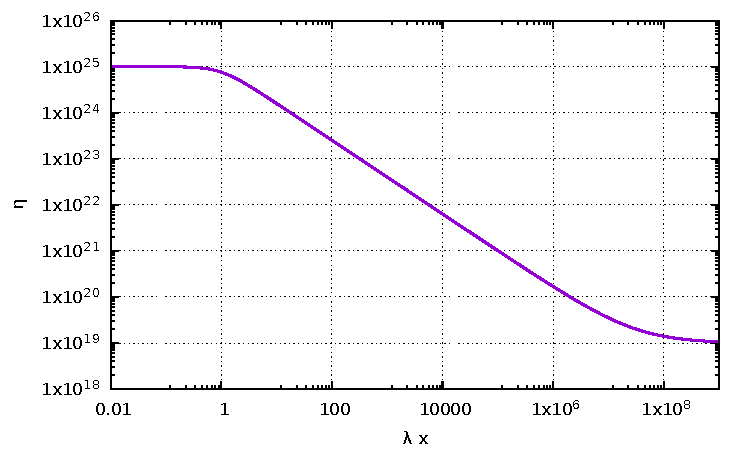
\includegraphics[width=7cm]{images/rheology/carreau/carreau.pdf}
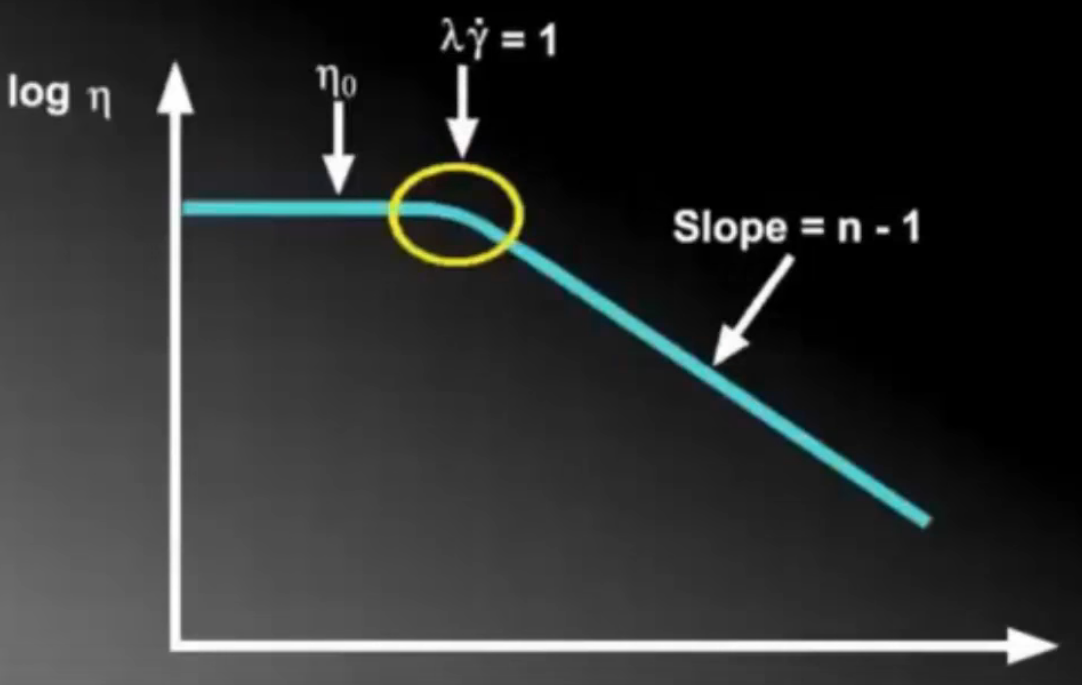
\includegraphics[width=6cm]{images/rheology/carreau/carreau1}\\
{\captionfont Left: Carreau model effective viscosity as a function of 
the product $\lambda \dot{\varepsilon}_{e}$. Right: taken from 
video at \url{https://youtu.be/qErs5zZV4BQ}.}
\end{center}

Note that the (Bird)-Carreau-Yasuda model \cite{yaac81,osru14} is very similar to the standard (Bird)-Carreau:
\begin{equation}
\eta = \eta_\infty + (\eta_0-\eta_\infty) \left(1 + (\lambda \dot{\varepsilon}_{e})^a \right)^{(n-1)/a}
\end{equation}
It is for instance used in van de Vosse \etal (2003) \cite{vadv03} to model blood.
\index{general}{Bird-Carreau-Yasuda model}

Flows in a Lid-Driven Cavity with this rheology are presented in \cite{zifr07,shal09}.

\Literature: Bercovici (1993) \cite{berc93}, Bercovici (1995) \cite{berc95},
Marcotte (2000) \cite{marc00}, Huerta \& Liu (1988) \cite{huli88}.

%------------------------------
\subsubsection{Bingham model} \label{sec:bingham}
\index{general}{Bingham model}

Bingham \cite{bingham} fluids can sustain an applied stress without any motion occuring. Only when the applied stress exceeds
a yield stress $\tau_0$ then the fluid flows. This translates as follows \cite{reddybook2}:

\begin{eqnarray}
{\bm \tau} &=& \left(  \frac{\tau_0}{\dot{\varepsilon}} + 2 \eta_0  \right)\dot{\bm \varepsilon}^d \qquad 
\text{ if } {\tau}_{e}>\tau_0 \\
{\bm \tau} &=& {\bm 0} \qquad\qquad\qquad\qquad  \text{if } \tau_{e} \leq \tau_0 
\end{eqnarray}
When flow occurs, the effective viscosity is then given by:
\begin{equation}
\eta(\dot{\varepsilon}_e) = \frac{\tau_0}{\dot{\varepsilon}_e} + 2 \eta_0 
\end{equation}
and when the strain rate is large we recover a Newtonian behaviour.
Typical Bingham fluids are mud, slurry, toothpaste.  

When using a velocity-based FEM code, the implementation of this rheological behaviour 
is complicated by the no-flow condition under a given stress. However, our codes
require a relationship between stress and strain rate in the form of an effective viscosity
which cannot be zero. 
This difficulty can be circumvented by implementing Bingham fluids as follows \cite{reddybook2}:

\begin{eqnarray}
{\bm \tau} &=& \left(  \frac{\tau_0(1-\eta/\eta_r)}{\dot{\varepsilon}_e} 
+ 2 \eta_0  \right)\dot{\bm \varepsilon} \qquad \text{ if } \tau_{e}>\tau_0 \\
{\bm \tau} &=& 2 \eta_r \dot{\bm \varepsilon}  \qquad\qquad\qquad\qquad\qquad\qquad  
\text{if } \tau_{e} \leq \tau_0 
\end{eqnarray}
where $\eta_r$ is a pre-yield viscosity and $\eta/\eta_r<<1$ (typically 1\% or less). This is a form of 
regularisation, and we will see a similar one in the next section.

Note the interesting paper by Barnes and Walter (1985) \cite{bawa85} who argue that 
"the yield stress concept is an idealization, and that, given accurate
measurements, no yield stress exists. The simple Cross model is shown to be a
useful empiricism for many non-Newtonian fluids, including those which have
hitherto been thought to possess a yield stress." The Cross model is presented 
in Section~\ref{ss:cross}.
 

\Literature: 
Papanastasiou (1987) \cite{papa87}, Blackery \& Mitsoulis (1997) \cite{blmi97},
Mitsoulis \& Zisis (2001) \cite{mizi01}, Mahmood \etal (2017) \cite{maky17},
Syrakos \etal (2014) \cite{syga14}, Bingham \cite{bingham}, Balmforth \& Rust (2009) \cite{baru09}, 
Grinevich \& Olshanskii (2009) \cite{grol09}, Sverdrup \etal (2018) \cite{svna18}
FE method for incompressible non-Newtonian flow (Bercovier \& Engelman (1980) \cite{been80});
Flow around a rigid sphere (Liu \etal (2002) \cite{limd02})

%------------------------------
\subsubsection{Herschel-Bulkley visco-plastic model}
\index{general}{Herschel-Bulkley model}

The Herschel-Bulkley model is effectively a combination of the power-law model and 
a simple plastic model:
\begin{eqnarray}
{\bm \tau} &=& 2 \left(  K \dot{\varepsilon}_e^{n-1} 
+ \frac{\tau_0}{\dot{\varepsilon}}\right)\dot{\bm \varepsilon} \qquad \text{ if } {\tau}_{e}>\tau_0 \\
\dot{\bm \varepsilon} &=& {\bm 0} \qquad\qquad \text{if }{\tau}_{e} \leq \tau_0 
\end{eqnarray}
in which $\tau_0$ is the yield stress, $K$ the consistency, and $n$ is the flow index \index{general}{Flow Index} \cite{demj04}.
The flow index measures the degree to which the fluid is shear-thinning ($n<1$) or shear-thickening ($n>1$).
If $n=1$ and $\tau_0=0$ the model reduces to the Newtonian model. 

The term between parenthesis above is the nonlinear effective viscosity. 
Concretely, the implementation goes as 
follows\footnote{\url{https://en.wikipedia.org/wiki/Herschel-Bulkley_fluid}}:
\begin{equation}
\eta(\dot{\bm \varepsilon}) = 
\left\{
\begin{array}{cc}
\eta_0 & \dot{\varepsilon}_e\leq \dot{\varepsilon}_0 \\ 
K \dot{\varepsilon}_e^{n-1} + \frac{\tau_0}{\dot{\varepsilon}_e} & \dot{\varepsilon}_e \geq \dot{\varepsilon}_0
\end{array}
\right.
\end{equation}
The limiting viscosity $\eta_0$ is chosen such that 
$\eta_0 =  K \dot{\varepsilon}_0^{n-1} + \frac{\tau_0}{\dot{\varepsilon}_0}$

A large limiting viscosity means that the fluid will only flow in response to a large applied force. 
This feature captures the Bingham-type behaviour of the fluid. 
Note that when strain rates are large, the power-law behavior dominates. 

As we have seen for Bingham fluids, the equations above are not easily amenable to implementation so that 
one usually resorts to regularisation, which is a modification of the 
equations by introducing a new material parameter which controls the exponential 
growth of stress. This way the equation is valid for both yielded 
and unyielded areas (Blackery \& Mitsoulis (1997) \cite{blmi97},
Papanastasiou (1987) \cite{papa87}, Zinani \& Frey (2007) \cite{zifr07}, 
Sverdrup \etal (2018) \cite{svna18}):
\begin{equation}
\eta(\dot{\varepsilon}_e) 
= K \dot{\varepsilon}_e^{n-1} + \frac{\tau_0}{\dot{\varepsilon}_e} [1 - \exp(-m \dot{\varepsilon}_e)] 
\end{equation}
When the strain rate becomes (very) small a Taylor expansion of the regularisation 
term yields $1- \exp(-m \dot{\varepsilon}) \sim m \dot{\varepsilon} $ so that 
$\eta_{eff} \rightarrow m \tau_0$.
However, it seems more physically meaningful to replace $m$ by a reference strain 
rate value $\dot{\varepsilon}_0$ so that 
\begin{mdframed}[backgroundcolor=blue!5]
\begin{equation}
\eta_{eff}(\dot{\bm \varepsilon}) 
= K \dot{\varepsilon}_e^{n-1} + \frac{\tau_0}{\dot{\varepsilon}_e} 
\left[1 - \exp\left(-\frac{\dot{\varepsilon}_e}{\dot{\varepsilon}_0} \right) \right]
\end{equation}
\end{mdframed}
In this case, when strain rate becomes (very) small a Taylor expansion of the regularisation
term yields
\begin{equation}
\frac{\tau_0}{\dot{\varepsilon}_e} \left[1 - 
\exp\left(-\frac{\dot{\varepsilon}_e}{\dot{\varepsilon}_0} \right) \right]
\simeq 
\frac{\tau_0}{\dot{\varepsilon}_e} \frac{\dot{\varepsilon}_e}{\dot{\varepsilon}_0}
=\frac{\tau_0}{\dot{\varepsilon}_0} 
\end{equation}
This has the dimensions of a viscosity and this is effectively the definition 
of a maximum viscosity $\eta_{max}$.

\noindent\Literature: 
\begin{itemize}
\item Viscous flow with large free surface motion (Huerta \& Liu (1988) \cite{huli88});
\item Numerical simulation of thermal plumes (Massmeyer \etal \cite{madd13}); 
\item Flows Through a Sudden Axisymmetric Expansion (Machado \etal \cite{mazf}, 
      Jay \etal (2001) \cite{jamp01}); 
\item Dam break problem (Ancey \& Cochard (2009) \cite{anco09}, 
      Cochard \& Ancey (2009) \cite{coan09}, Balmforth \etal \cite{bafp09};
\item Weakly compressible Poiseuille flow (Taliadorou (2009) \cite{tagm09});
\item Flow past cylinders in tubes (Mitsoulis \& Galazoulas (2009) \cite{miga09});
\item Determination of yield surfaces (Burgos \& Alexandrou (1999) \cite{buae99});
\item Carbopol hydrogel rheology for experimental
      tectonics and geodynamics (Di Giuseppe \etal (2015) \cite{dicf15}).
\item Flow past a sphere(disc) (Deglo de Besses \etal (2004) \cite{demj04}, 
      Gavrilov \etal (2017) \cite{gafp17}). \mscthesis\index{general}{MSc Thesis} 
\end{itemize}


%...........................................................
\subsubsection{The Casson model}

It is described in Barnes (1999) \cite{barn99}:
\begin{equation}
\sqrt{\sigma} = \sqrt{\sigma_y} + \sqrt{\eta_p \dot{\varepsilon}_e} 
\end{equation}
or, when squaring it:
\begin{equation}
\sigma = \sigma_y + \eta_p \dot{\varepsilon}_e + 2\sqrt{\sigma_p \eta_p \dot{\varepsilon}_e} 
\end{equation}
This model has been found to accurately describe the behaviour of synthetic based muds \cite{adlo17}. 

%-------------------------------------------------
\subsubsection{The Ellis model\label{ss:ellis}}

An Ellis equation would be of the form \cite{robc01} 
\begin{equation}
\frac{\eta-\eta_\infty}{\eta_0-\eta_\infty} =
\frac{1}{1+(\sigma/\sigma_c)^m}
\end{equation}
where $\sigma$ is the shear stress, $\sigma_c$ is a critical shear stress
and $m$ is a large number. 

%-------------------------------------------------
\subsubsection{One model to rule them all? \label{ss:cross}}

Let us consider the base equation
\begin{equation}
\boxed{
\frac{\eta-\eta_\infty}{\eta_0-\eta_\infty} = 
\left[ 1+(K \dot{\varepsilon}_e)^a  \right]^{-(1-n)/a}
}
\end{equation}
This equation is purposefully generic and specific parameter combination choices 
allow to recover any of the above models (and more) \cite{osru14}.
See also an early paper by Cross (1965) \cite{cros65} for a somewhat similar equation. 

%\begin{itemize}
%\item Newtonian:  $K=0$ is sufficient
%\item power-law: $\eta << \eta_0$, $\eta >> \eta_\infty$, $a=1$:
%\end{itemize}
Similar conclusions are reached in the following video:
\begin{center}
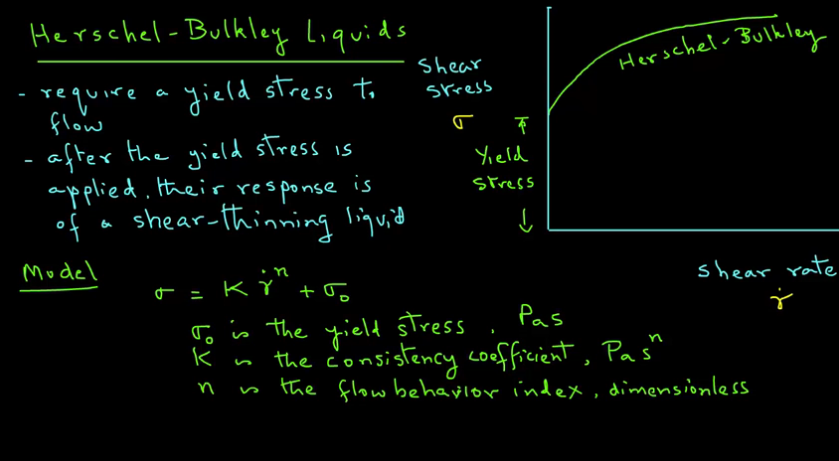
\includegraphics[width=7cm]{images/rheology/hbyoutube}\\
{\captionfont \url{https://youtu.be/dVCb11dZR7Y}}
\end{center}

%-------------------------------------------------
\subsubsection{Dislocation and Diffusion creep}
\index{general}{Dislocation creep}
\index{general}{Diffusion creep}

\todo[inline]{insert here background and links to relevant textbooks}

The standard dislocation creep effective viscosity is given by:
\begin{mdframed}[backgroundcolor=blue!5]
\[
\eta^{ds}(p,T,\dot{\bm \varepsilon})
=\eta^{ds}(p,T,\dot{\varepsilon}_e)
= \frac{1}{2} f A^{-1/n} \dot{\varepsilon}_{e}^{(1-n)/n} \exp \left( \frac{Q+pV}{nRT}  \right)
\] 
\end{mdframed}
where $A$ is the pre-exponential scaling factor, $f$ is a scaling factor
representing viscous weakening or strengthening, $Q$ is the activation energy, 
$V$ is the activation volume, $T$ is the absolute temperature, $n$ is the power-law 
exponent, $R$ is the universal gas constant. 

The coefficients $A,n,Q,V$ are material parameters and are obtained in the laboratory 
by means of high pressure/temperature experiments (see for instance Karato \& Wu (1993) \cite{kawu93}). 
Unfortunately these experiments cannot be run at Earth-like strain rate 
values ($\sim 10^{-15}\si{\per\second}$)
so that extrapolations must be carried out over several orders of magnitude to 
arrive at values we can use in our numerical models. 
The 1/2 factor arises from the relationship between deviatoric stress and strain rate which 
involves a factor 2.

The factor $f$ is in fact a tuning parameter used to explore end members (e.g. 'weak crust' 
vs 'strong crust'), see discussion in the supplementary material in 
Huismans \& Beaumont (2011) \cite{hube11}. 
This approach has been extensively used by the \sopale users community, see 
for instance Warren \etal (2008) \cite{wabj08,wabj08b,wabj08c} 
or Gray \& Pysklywec (2012) \cite{grpy12}.

\todo[inline]{insert here equation for diffusion creep}

Furthermore, we know that several other factors will strongly affect the rheology:
\begin{itemize}
\item water content, or as often mentioned: 'dry' vs 'wet'. Following \cite{kawu93}, 
dry means water-free and wet means water-saturated conditions.
\begin{center}
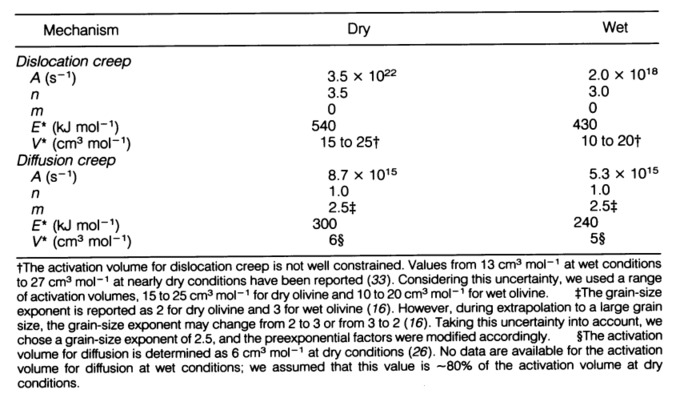
\includegraphics[width=8cm]{images/rheology/kawu93}\\
{\captionfont Taken from Karato and Wu \cite{kawu93}.}
\end{center}
\Literature: Quinquis \& Buiter (2014) \cite{qubu14} and refs therein for the effects of water
migration on models of subduction dynamics.

\item composition: while one typically assigns olivine properties to the mantle in models, 
the mineral olivine\footnote{\url{https://en.wikipedia.org/wiki/Olivine}} 
is actually a magnesium iron silicate with the formula (Mg$^{2+}$, Fe$^{2+}$)$_2$SiO$_4$.
and the ratio of magnesium to iron varies between the two endmembers of the solid solution series: 
forsterite (Mg-endmember: Mg$_2$SiO$_4$) and fayalite (Fe-endmember: Fe$_2$SiO$_4$).

\item grain size: this only affects diffusion creep mechanisms \cite{kawu93}. 
Grain size varies over several orders of magnitude and also evolves over time and 
its evolution is affected by the ambient deformation and the deformation history.
Dannberg \etal \cite{daef17} then used a diffusion creep effective viscosity 
given by:
\[
\eta^{df} = \frac{1}{2} A_{df}^{-1} d^m \exp \left( \frac{Q_{df}+pV_{df}}{RT}  \right)
\] 
where $d$ is the (variable) grain size and $m$ the grain size exponent. Grain growth/evolution 
is usually approximated using semi-empirical expressions \cite[section~2.2]{daef17}.
Smaller grains facilitating faster creep.

Relevant literature on this topic is in Section~\ref{sec:topics:gsev}.

\item anisotropy, LPO: see relevant literature in Section \ref{sec:topics:anisotropy}.

\item phase changes 
\end{itemize}

\begin{remark}
It is not uncommon to find in the literature effective viscosity formulations written as a function 
of $B$ with $B=A^{-1/n}$ \cite{wabj08,wabj08b,wabj08c}. Also, this $B$ coefficient often contains the conversion 
factor of the next remark.
\end{remark}

\begin{remark} Material parameters obtained in the lab are often measured on a uniaxial machine. 
An additional coefficient is added to the effective viscosity formula (see \cite{grpy12,grpy13}, 
or Table 1a of Warren \etal (2008) \cite{wabj08}):
$3^{-(1+n)/2n}2^{(1-n)/n}$. See page 77 of Ranalli \cite{ranalli} for an explanation.
\end{remark}

\begin{center}
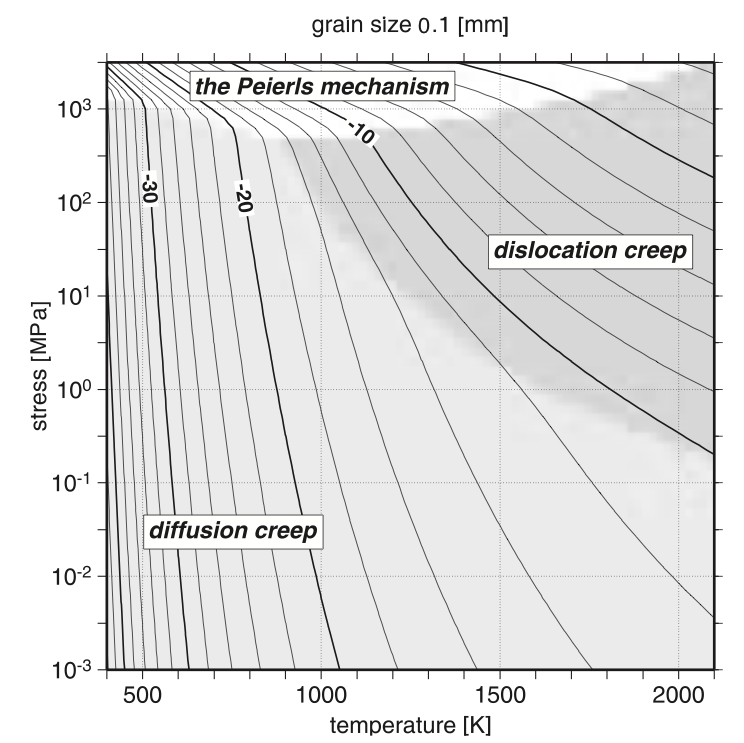
\includegraphics[width=7cm]{images/rheology/defmap}
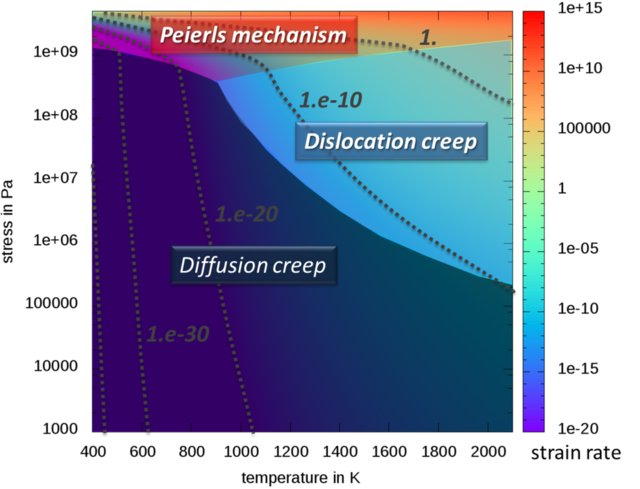
\includegraphics[width=9cm]{images/rheology/elme18}\\
{\captionfont 
Fig-$\mathds{B}$: Left: Taken from Kameyama \etal (1999) \cite{kayk99}.
Deformation mechanism map calculated for grain size $a=0.1\si{mm}$. The lightly shaded area indicates 
that deformation mainly occurs by diffusion creep. The densely shaded area indicates that 
deformation mainly occurs by power-law creep. 
The white region indicates that deformation mainly occurs by the Peierls mechanism. The 
solid curves are lines of constant strain rate. The numbers attached to each contour indicate the 
logarithm of the strain rate in the unit of $\si{\per\second}$.
Right: Taken from Elbeshausen \& Melosh (1998) \cite{elme18}. 
Strain rate as a function of stress and temperature. The parameter space dominated by each of 
the terms is denoted by different hues, depending on strain rate. Note that the original equations 
implicitly include a pressure dependence in the enthalpy term, which is not strong and 
therefore neglected here. The diffusion regime is highly temperature dependent and 
important for small strain rates only. Dislocation creep occurs for intermediate 
stresses and higher temperatures, while the Peierls mechanism dominates at higher stresses 
($\ge 500\si{\mega\pascal})$ and shows a strong stress dependence for low temperatures. 
The dashed contours are strain rate in units of $\si{\per\second}$. 
}
\end{center}


\paragraph{A closer look at the diffusion creep of Karato \& Wu (1993)} In the article, 
the following equation is used: 
\[
\dot{\bm \varepsilon} = 
A \left(\frac{{\bm \tau}}{\mu}\right) \left(\frac{b}{d}\right)^m \exp \left( -\frac{Q+pV}{RT}\right)
\]
where $\mu$ is the shear modulus ($\sim$80\si{\giga\pascal}), 
$b$ is the length of the Burgers vector ($\sim$0.5\si{\nano\metre}) and 
$d$ is the grain size.
One can express the above equation in terms of second invariants (see Section~\ref{sec:invariants}):
\[
\underline{\dot{\varepsilon}}_{e} 
= A \left(\frac{\underline{\tau}_{e}}{\mu}\right) \left(\frac{b}{d}\right)^m \exp\left( -\frac{Q+pV}{RT} \right)
\]
and assuming a Newtonian linearisation/relation between deviatoric stress 
and strain rate  $\underline{\tau}_{e} = 2 \eta^{df} \underline{\dot\epsilon}_{e}$, one arrive at
\[
\eta^{df} = \frac{1}{2} \left(\frac{A}{\mu}\right)^{-1}  
\left(\frac{b}{d}\right)^{-m} \exp\left( \frac{Q+pV}{RT} \right)
\]
or, 
\[
\eta^{df} = \frac{1}{2} \left[ \frac{A}{\mu}   
\left(\frac{b}{d}\right)^{m} \right]^{-1} \exp\left( \frac{Q+pV}{RT} \right)
\]
The effective diffusion creep viscosity is independent of strain-rate so that one 
could substitute the total pressure for lithostatic pressure in the equation, assume 
a geotherm and easily compute the predicted viscosity as a function of grain size $d$.

Let us assume that the 1D profile starts from the base of the lithosphere 
(say 120\si{\km} depth) and ends at the 660 boundary. 
Assume the temperature to increase linearly from 1300\degree C to $T_{bottom}$ (to 
be specified). At the bottom 
of the lithosphere, the lithostatic pressure is of the order of 
$\rho \cdot g \cdot L \simeq 3000\cdot 10 \cdot 120e3 \simeq 4$\si{\giga\pascal}. 
At the bottom of the domain, the pressure has increased 
by $3300\cdot 10 \cdot 630e3 \simeq21$\si{\giga\pascal}. 

The viscosity profile is plotted hereunder for three different grain sizes, bottom temperature and 
activation volumes (4,5,6 cm$^3$/mol). 

\begin{center}
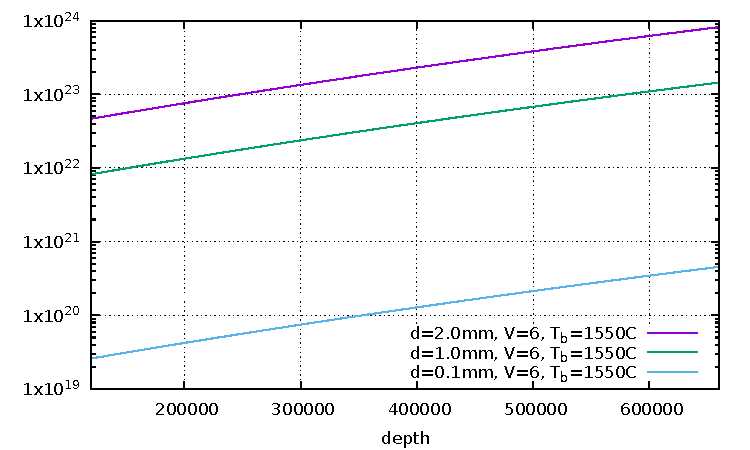
\includegraphics[width=5.cm]{images/rheology/kawudiff/viscosity1.pdf}
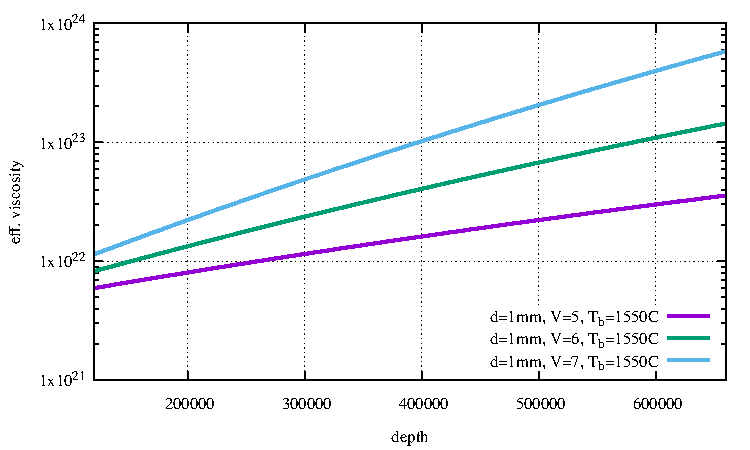
\includegraphics[width=5.cm]{images/rheology/kawudiff/viscosity2.pdf}
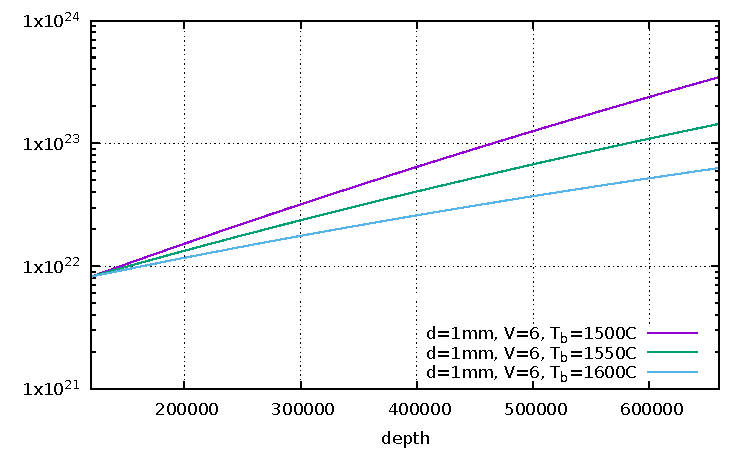
\includegraphics[width=5.cm]{images/rheology/kawudiff/viscosity3.pdf}\\
{\captionfont Effective diffusion creep viscosity for various 
grain size, activation volume and basal temperature values.}\\
{\color{gray} \tiny {images/rheology/kawudiff/}}
\end{center}

Although this exercise only provides us with first-order results, we can conclude that 
one can essentially change the diffusion creep effective viscosity by up to 2 orders of 
magnitude simply by choosing key parameters within acceptable ranges. 


%------------------------------
\subsubsection{The von Mises failure criterion}\label{sec:vMcriterion}
\index{general}{von Mises}
\begin{flushright} {\tiny {\color{gray} vMcriterion.tex}} \end{flushright}
%~~~~~~~~~~~~~~~~~~~~~~~~~~~~~~~~~~~~~~~~~~~~~~~~~~~~~~~~~~~~~~~~~~~~~~~~~~~~~~~~~~~~~~~~~~~~~~~~~~

The von Mises yield criterion suggests that the yielding of materials begins when the second 
deviatoric stress invariant ${\cal I}_2({\bm \tau})$ reaches a critical value. 
For this reason, it is sometimes called the $J_2$-plasticity or $J_2$ flow 
theory\footnote{$J_2$ is the common notation for ${\cal I}_2({\bm \tau})$}. 
It is part of a plasticity theory that applies best to ductile materials, such as metals. 

In material science and engineering the von Mises yield criterion can be also formulated in terms of 
the von Mises stress or equivalent tensile stress, $\sigma_v$, a scalar stress value that can be computed 
from the stress tensor. In this case, a material is said to start yielding when its von Mises stress 
reaches a critical value known as the yield strength, $\sigma_Y$. The von Mises stress is used to predict 
yielding of materials under any loading condition from results of simple uniaxial tensile tests. The 
von Mises stress satisfies the property that two stress states with equal distortion energy have equal 
von Mises stress. 

Because the von Mises yield criterion is independent of the first stress 
invariant, ${\cal I}_1({\bm \sigma})$, it is applicable 
for the analysis of plastic deformation for ductile materials such as metals, as the 
onset of yield for these materials does not depend on the hydrostatic component of the stress tensor. 

Although formulated by Maxwell in 1865, it is generally attributed to von Mises \cite{vonm13}. 
Huber (1904), in a paper in Polish, anticipated to some extent this criterion. 
Heinrich Hencky formulated the same criterion as von Mises independently in 1924 \cite{henc24,tata03}.
This criterion is also referred to as the Maxwell-Huber-Hencky-von Mises theory. 

The von Mises yield criterion (also known as Prandtl-Reuss yield criterion) 
is expressed in the principal stresses as
\[
\sqrt{{\cal I}_2({\bm \tau})} = c \quad \text{or}, \quad 
\frac{1}{6}[(\sigma_1 - \sigma_2)^2 + (\sigma_2 - \sigma_3)^2 + (\sigma_3 - \sigma_1)^2] =  c^2 
\]
where $c$ is the yield stress in uniaxial tension.
The von Mises yield criterion writes:

\begin{mdframed}[backgroundcolor=blue!5]
\begin{equation}
F^{\text{\tiny VM}}= \sqrt{{\cal I}_2({\bm \tau})  } - c  \label{vmcrit}
\end{equation}
\end{mdframed}
which is the Drucker-Prager criterion with $\phi=0$ (see Section~\ref{sec:dpcriterion}).

The following figure shows the von Mises yield surface in the three-dimensional space of principal stresses. 
\begin{center}
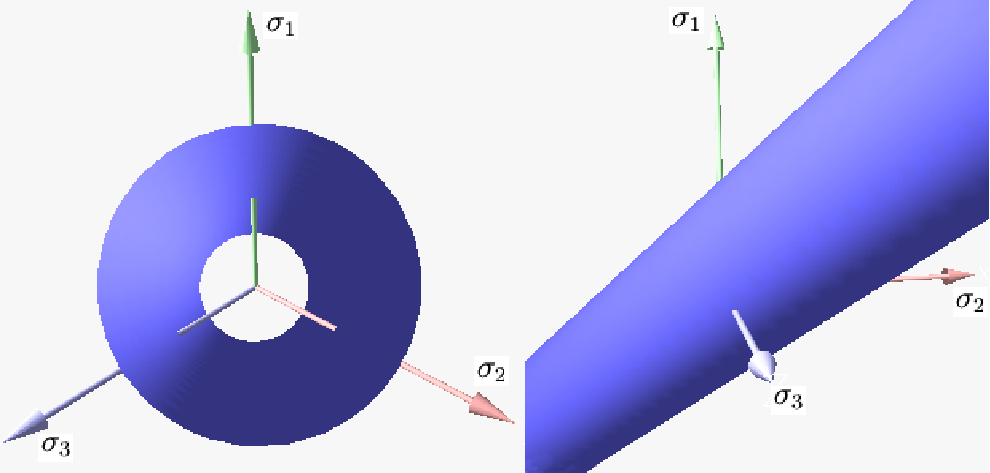
\includegraphics[width=0.6\textwidth]{images/rheology/vonmises/vonmises.pdf}\\
{\captionfont Most likely taken from Wikipedia...}
\end{center}
It is a circular cylinder of infinite length with its axis inclined at equal angles to the three principal stresses. 

\Literature: 
\fullcite{papa87}, \fullcite{ting03}

%\begin{center}
%\includegraphics[width=0.6\textwidth]{RHEOLOGY/viscoplasticity/vMcriterion.pdf}
%\end{center}
\paragraph{The yield surface} Let us try to draw the yield function in 
the space $\sigma_1,\sigma_2,\sigma_3$. It is given by
\begin{eqnarray}
&&\sqrt{ {\cal I}_2({\bm \tau}) } = c \\
&\Rightarrow&  {\cal I}_2({\bm \tau})  = c^2 \\
&\Rightarrow& \frac{1}{6}\left[(\sigma_{1}-\sigma_{2})^2 + (\sigma_{2}-\sigma_{3})^2 
+ (\sigma_{1}-\sigma_{3})^2 \right] =c^2 \\
&\Rightarrow & (\sigma_{1}-\sigma_{2})^2 + (\sigma_{2}-\sigma_{3})^2 + (\sigma_{1}-\sigma_{3})^2 = 6c^2 
\end{eqnarray}
or, temporarily setting $x=\sigma_1$, $y=\sigma_2$ and $z=\sigma_3$: 
\begin{eqnarray}
(x-y)^2 + (y-z)^2 + (x-z)^2 &=& 6c^2 \\
(x-y)^2 + y^2 - 2yz + z^2 + x^2 -2xz +z^2 &=& 6c^2\\
2z^2 - 2(x+y)z + (x-y)^2+x^2+y^2-6c^2 &=& 0
\end{eqnarray}
This is a second order polynomial in $z$. Its discriminant $\Delta$ is
\begin{eqnarray}
\Delta 
&=& 4(x+y)^2 - 4 \cdot 2 \cdot [(x-y)^2+x^2+y^2-6c^2] \nn\\
&=& 4x^2 + 8xy + 4y^2 - 8 [x^2-2xy+y^2 +x^2+y^2-6c^2] \nn\\
&=& 4x^2 + 8xy + 4y^2 - 8 [2x^2-2xy+2y^2 -6c^2] \nn\\
&=& 4x^2 + 8xy + 4y^2 - 16x^2+ 16xy -16y^2 +48 c^2 \nn\\
&=& -12x^2 + 24xy -12 y^2  +48 c^2 \nn\\
&=& -12(x^2 -2xy + y^2)  + 48 c^2 \nn\\
&=& -12(x-y)^2  + 48 c^2 \nn
\end{eqnarray}
Since I am looking for $z(x,y)\in \mathbb{R}$ then $\Delta >0$ and this 
imposes a restriction on admissible $x,y$ pairs:
\[
 -12(x-y)^2  + 48 c^2 \nn > 0
\]
\[
(x-y)^2  < 4 c^2 
\]
\[
x-y<2c   
\qquad
\text{or,}
\qquad
y-x<2c   
\]
\[
y> x-2c   
\qquad
\text{or,}
\qquad
y<x+2c
\]
So the discriminant is positive in the band given by $y>x-2c$ and $y<x+2c$ in the $x,y$-plane, 
which is a band centered around the line $y=x$.
When $\Delta>0$ we have then 
\[
z= \frac{2(x+y) \pm \sqrt{\Delta}}{4}
\]
which means that for each pair $x,y$ there are 2 $z$ values. 
The middle of this surface is given by the line $z=(x+y)/2$. 
The plane normal to this line is given by $z=-2(x+y)$.

This approach is reasonably simple for the von Mises criterion but 
quickly becomes intractable for other criteria.

\vspace{.5cm}

We now look into the derivatives of the von Mises plastic potential $Q^{\text{\tiny vM}}(\bm\sigma)$.
We have
\begin{equation}
Q^{\text{\tiny vM}}(\bm\sigma) =\sqrt{{\cal I}_2({\bm \tau})  } - c  
\end{equation}
Then
\begin{eqnarray}
\frac{\partial Q^{\text{\tiny vM}} }{\partial {\cal I}_1(\bm\sigma)} &=& 0 \\
\frac{\partial Q^{\text{\tiny vM}} }{\partial \sqrt{{\cal I}_2(\bm\tau)}}&=& 1 \\
\frac{\partial Q^{\text{\tiny vM}} }{\partial \theta_{\rm L}(\bm\tau)} &=& 0 
\end{eqnarray}
so 
\begin{eqnarray}
C_1^{\text{\tiny vM}} &=& 0  \\ 
C_2^{\text{\tiny vM}} 
&=& \frac{1}{2  \sqrt{{\cal I}_2(\bm\tau)}   } (1-0) 
= \frac{1}{2  \sqrt{{\cal I}_2(\bm\tau)}   } \\ 
C_3^{\text{\tiny vM}} &=& 0  
\end{eqnarray}


\newpage


%------------------------------
\subsubsection{The Tresca failure criterion}
\index{general}{Tresca}
The Tresca or maximum shear stress yield criterion is taken to be the work of Henri Tresca. It is also referred as the Tresca-Guest (TG) criterion. The functional form of this yield criterion is
\[
f(\sigma_1,\sigma_2,\sigma_3) = 0
\]
In terms of the principal stresses the Tresca criterion is expressed as
\[
{\max(|\sigma_1 - \sigma_2| , |\sigma_2 - \sigma_3| , |\sigma_3 - \sigma_1| ) = \sigma_0 }
\]
The following figure shows the Tresca-Guest yield surface in the three-dimensional space of principal stresses. 
\begin{center}
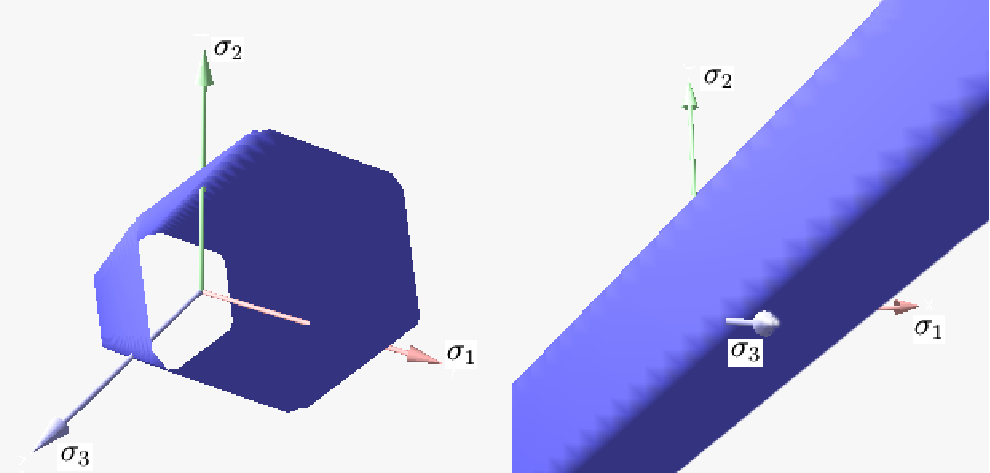
\includegraphics[width=0.6\textwidth]{images/rheology/tresca/Tresca.pdf}
\end{center}
It is a prism of six sides and having infinite length. This means that the material remains viscous when all three principal stresses are roughly equivalent (a hydrostatic pressure), no matter how much it is compressed or stretched. However, when one of principal stresses becomes smaller (or larger) than the others the material is subject to shearing. In such situations, if the shear stress reaches the yield limit then the material enters the plastic domain. 

\begin{remark}
The yield function is non-continuous, making its numerical implementation more difficult (directional derivatives are needed)
\end{remark}

%%%%%%%%%%%%%%%%%%%%%%%%%%%%%%%%%%
\paragraph{two-dimensional space}
Using the values of the principal stresses in a two dimensional space, the criterion becomes 
\[
|\sigma_1 - \sigma_2| =\sqrt{J_2'}  = \sigma_0 
\]
which is equivalent to the von Mises criterion.


%%%%%%%%%%%%%%%%%%%%%%%%%%%%%%%%%%
\paragraph{three-dimensional space}
We have already established that 
\begin{eqnarray}
\sigma_1 - \sigma_3  &=& 2 \sqrt{J_2} \cos \theta \nn
\end{eqnarray}
with $\sigma_1>\sigma_>\sigma_3$,
so that the failure criterion is given by

\begin{mdframed}[backgroundcolor=blue!5]
\[
F^{TR,3D}=2\sqrt{J_2}\cos \theta - c 
\]
\end{mdframed}

Obviously, the Tresca criterion corresponds to the case where the friction angle $\phi=0$.


\Literature: \cite{long03}


%------------------------------
\subsubsection{The Mohr-Coulomb failure criterion}
\index{general}{Mohr-Coulomb}
\begin{flushright} {\tiny {\color{gray} mccriterion.tex}} \end{flushright}
%~~~~~~~~~~~~~~~~~~~~~~~~~~~~~~~~~~~~~~~~~~~~~~~~~~~~~~~~~~~~~~~~~~~~~~~~~~~~~~~~~~~~~~~~~~~~~~~~~~

Mohr-Coulomb theory is a model describing the response of a material such as rubble piles or concrete to shear stress as well as normal stress. 
Most of the classical engineering materials somehow follow this rule in at least a portion of their shear failure envelope. In geology it is used to define shear strength of soils at different effective stresses \cite{hand69}.

In structural engineering it is used to determine failure load as well as the angle of fracture of a displacement fracture in concrete and similar materials. Coulomb's friction hypothesis is used to determine the combination of shear and normal stress that will cause a fracture of the material. Mohr's circle is used to determine the principal stresses that will produce this combination of shear and normal stress, and the angle of the plane in which this will occur. According to the principle of normality, the stress introduced at failure will be perpendicular to the line describing the fracture condition.

%It can be shown that a material failing according to Coulomb's friction hypothesis will show the displacement introduced at failure forming an angle to the line of fracture equal to the angle of friction. This makes the strength of the material determinable by comparing the external mechanical work introduced by the displacement and the external load with the internal mechanical work introduced by the strain and stress at the line of failure. By conservation of energy the sum of these must be zero and this will make it possible to calculate the failure load of the construction.

The Mohr-Coulomb failure criterion represents the linear envelope that is obtained from a plot of the shear strength of a material 
versus the applied normal stress. This relation is expressed as (Owen \& Hinton book \cite[p219]{owhi})
%\[
%\tau = c- \sigma~\tan(\phi) 
%\]

%Compression is assumed to be positive in the following discussion. If compression is assumed to be negative then $\sigma$ should be replaced with $-\sigma$.

%If $\phi=0$, the Mohr-Coulomb criterion reduces to the Tresca criterion. On the other hand, if $\phi = 90^\circ$ the Mohr-Coulomb model is equivalent to the Rankine model. Higher values of $\phi$ are not allowed.

\begin{equation}
\tau_m = -\sigma_m \sin \phi + c \cos \phi  \label{eq:mccrit}
\end{equation}
where $\tau_m$ is the magnitude of the shear stress, 
$\sigma_m$ is the normal stress, $c$ is the intercept of the failure envelope with the $\tau$ axis, 
and $\phi$ is the slope of the failure envelope.
The minus sign in the above equation is for the case where compression is assumed to be 
negative\footnote{\url{https://en.wikipedia.org/wiki/Mohr-Coulomb_theory}}.
The quantity $c$ is often called the cohesion and the angle $\phi$ is called the angle of internal friction.
 
We have  
\[
\tau_m=\frac{\sigma_1-\sigma_3}{2}
\qquad
\qquad
\sigma_m = \frac{\sigma_1+\sigma_3}{2}
\]
with $\sigma_1$ is the maximum principal stress and $\sigma_3$ is the minimum principal stress, or
%\[
%\sigma_1-\sigma_3 = - ( \sigma_1+\sigma_3) \sin \phi + 2c \cos \phi
%\]
%\[
%\sigma_1-\sigma_3 = 2 c \cos \phi - (\sigma_1+\sigma_3) \sin\phi
%\]
\begin{equation}
\cfrac{\sigma_1-\sigma_3}{2} = -\cfrac{\sigma_1+\sigma_3}{2}~\sin\phi +c\; \cos\phi 
\end{equation}
Using Eqs.~\eqref{eq:sig13a} and \eqref{eq:sig13b} 
for $(\sigma_1 - \sigma_3 )/2$ and $(\sigma_1 + \sigma_3 )/2$:
\begin{eqnarray}
&& \frac{\sigma_1 - \sigma_3}{2} = -\frac{\sigma_1 + \sigma_3}{2} \sin \phi  + c \cos \phi \nn\\
&\Rightarrow&
\sqrt{  {\cal I}_2({\bm \tau}) } \cos \theta = -\left(\frac{1}{3}{\cal I}_1({\bm \sigma}) - \sqrt{  {\cal I}_2({\bm \tau})} \frac{1}{\sqrt{3}} \sin \theta \right) \sin \phi 
+ c \cos \phi \nn\\
&\Rightarrow&
\frac{1}{3} {\cal I}_1({\bm \sigma}) \sin \phi  
+ \sqrt{  {\cal I}_2({\bm \tau}) } \left( \cos \theta - \frac{1}{\sqrt{3}} \sin \theta  \sin \phi \right) - c \cos \phi = 0 \nn
\end{eqnarray}

\begin{mdframed}[backgroundcolor=blue!5]
\begin{equation}
F^{\text{\tiny MC}}=\frac{1}{3} {\cal I}_1({\bm \sigma}) \sin \phi  + 
\sqrt{  {\cal I}_2({\bm \tau})  } \left( \cos \theta - \frac{1}{\sqrt{3}} \sin \theta  \sin \phi \right) - c \cos \phi
\label{eq:mcF} 
\end{equation}
\end{mdframed}
This formula (without the cohesion) is used in \textcite{will92}.
Since $p=-\frac{1}{3} {\cal I}_1({\bm \sigma})$, we also have:
%\begin{equation}
%F^{\text{\tiny MC}}= -p \sin \phi  + 
%\sqrt{ {\cal I}_2({\bm \tau})  } \left( \cos \theta - \frac{1}{\sqrt{3}} \sin \theta  \sin \phi \right) - c \cos \phi 
%\end{equation}
%or, 
\begin{mdframed}[backgroundcolor=blue!5]
\begin{equation}
F^{\text{\tiny MC}}=
\sqrt{  {\cal I}_2({\bm \tau})  } \left( \cos \theta - \frac{1}{\sqrt{3}} \sin \theta  \sin \phi \right) - (p \sin\phi + c \cos \phi)
\end{equation}
\end{mdframed}

\begin{remark}
The expression for $F$ in the Mohr-Coulomb case in Zienkiewicz \& Cormeau (1974) \cite{zico74} 
contains errors which are later corrected in \textcite[p102]{book_zitf}. 
\end{remark}

\Literature: this criterion is also used in computer graphics animation \cite{zhbr05}

\todo{when $\phi=0$ we should recover Tresca but factor 2 is wrong ?}



\vspace{.5cm}

We now look into the derivatives of the Drucker-Prager plastic potential $Q^{\text{\tiny MC}}(\bm\sigma)$.
We have
\[
Q^{\text{\tiny MC}}=
\frac{1}{3} {\cal I}_1({\bm \sigma}) \sin \phi  + 
\sqrt{  {\cal I}_2({\bm \tau})  } \left(\cos\theta_{\rm L}(\bm\tau)-\frac{1}{\sqrt{3}} 
\sin\theta_{\rm L} (\bm\tau) \sin\phi \right) -c \cos \phi
\]
Then
\begin{eqnarray}
\frac{\partial Q^{\text{\tiny MC}}  }{\partial {\cal I}_1(\bm\sigma)} &=& \frac13 \sin\phi \\
\frac{\partial Q^{\text{\tiny MC}}  }{\partial \sqrt {{\cal I}_2(\bm\tau)}}
&=&  
\cos \theta_{\rm L} - \frac{1}{\sqrt{3}} \sin \theta_{\rm L}  \sin \phi  
+  \sqrt{  {\cal I}_2({\bm \tau})  } 
\left(-\sin \theta_{\rm L} - \frac{1}{\sqrt{3}} \cos \theta_{\rm L}  \sin \phi \right) 
\frac{\partial \theta_{\rm L}}{\partial \sqrt {{\cal I}_2(\bm\tau)}   } \nn \\
&=&  
\cos \theta_{\rm L} - \frac{1}{\sqrt{3}} \sin \theta_{\rm L}  \sin \phi  
+  \sqrt{  {\cal I}_2({\bm \tau})  } 
\left(-\sin \theta_{\rm L} - \frac{1}{\sqrt{3}} \cos \theta_{\rm L}  \sin \phi \right) 
\frac{\partial \theta_{\rm L}}{\partial  {{\cal I}_2(\bm\tau)}   }  
\frac{\partial   {{\cal I}_2(\bm\tau)}     }{\partial \sqrt {{\cal I}_2(\bm\tau)}   }  \nn\\
&=&  
\cos \theta_{\rm L} - \frac{1}{\sqrt{3}} \sin \theta_{\rm L}  \sin \phi  
+  \sqrt{  {\cal I}_2({\bm \tau})  } 
\left(-\sin \theta_{\rm L} - \frac{1}{\sqrt{3}} \cos \theta_{\rm L}  \sin \phi \right) 
\left(
-\frac12 \tan 3\theta_{\rm L} \frac{1}{ {\cal I}_2(\bm\tau)} 
\right)
2 \sqrt {{\cal I}_2(\bm\tau)} \nn \\
&=&  
\cos \theta_{\rm L} - \frac{1}{\sqrt{3}} \sin \theta_{\rm L}  \sin \phi  
+  
\left(\sin \theta_{\rm L} + \frac{1}{\sqrt{3}}\cos\theta_{\rm L}\sin\phi\right) \tan 3\theta_{\rm L} \nn\\
&=&  
\cos \theta_{\rm L}
\left[
1 - \frac{1}{\sqrt{3}} \tan \theta_{\rm L}  \sin \phi  
+  
\left(\tan \theta_{\rm L} + \frac{1}{\sqrt{3}}   \sin \phi \right)  \tan 3\theta_{\rm L} 
\right] \nn\\
&=&
\cos \theta_{\rm L}
\left[
(1 +  \tan \theta_{\rm L}   \tan 3\theta_{\rm L})
+\frac{1}{\sqrt{3}} \sin\phi
( \tan 3\theta_{\rm L} - \tan\theta_{\rm L})
\right]
\\ 
\frac{\partial Q^{\text{\tiny MC}} }{\partial \theta_{\rm L}(\bm\tau)} 
&=&  
\sqrt{{\cal I}_2(\bm \tau)} (-\sin\theta_{\rm L}-\frac{1}{\sqrt{3}} \cos\theta_{\rm L} \sin\phi )\nn\\
&=&  
-\frac{1}{\sqrt{3}} \sqrt{{\cal I}_2(\bm \tau)} (\sqrt{3} \sin\theta_{\rm L}+\cos\theta_{\rm L} \sin\phi )
\end{eqnarray}
so
\begin{eqnarray}
C_1^{\text{\tiny MC}} &=& \frac13 \sin\phi  \\ 
C_2^{\text{\tiny MC}} 
&=& 
\frac{1}{2 \sqrt{ {\cal I}_2(\bm\tau)}   }   
\left( \frac{\partial Q}{\partial \sqrt{{\cal I}_2(\bm\tau)}} 
- \frac{\tan 3\theta_{\rm L}}{\sqrt {{\cal I}_2(\bm\tau)}}
\frac{\partial Q}{\partial \theta_{\rm L}(\bm\tau)}  
\right) \nn\\
&=& 
\frac{1}{2 \sqrt{ {\cal I}_2(\bm\tau)}   }   
\left( \cos \theta_{\rm L} \left[
(1 +  \tan \theta_{\rm L}   \tan 3\theta_{\rm L})
+\frac{1}{\sqrt{3}} \sin\phi ( \tan 3\theta_{\rm L} - \tan\theta_{\rm L}) \right]
+ \frac{\tan 3\theta_{\rm L}}{\sqrt {{\cal I}_2(\bm\tau)}}
\frac{1}{\sqrt{3}} \sqrt{{\cal I}_2(\bm \tau)} (\sqrt{3} \sin\theta_{\rm L}+\cos\theta_{\rm L} \sin\phi )
\right) \nn\\
&=& 
\frac{1}{2 \sqrt{ {\cal I}_2(\bm\tau)}   }   
\left( \cos \theta_{\rm L}
\left[ (1 +  \tan \theta_{\rm L}   \tan 3\theta_{\rm L})
+\frac{1}{\sqrt{3}} \sin\phi
( \tan 3\theta_{\rm L} - \tan\theta_{\rm L}) \right]
+ \tan 3\theta_{\rm L}  ( \sin\theta_{\rm L}+\frac{1}{\sqrt{3}}\cos\theta_{\rm L} \sin\phi )
\right) \nn\\
&=& 
\frac{1}{2 \sqrt{ {\cal I}_2(\bm\tau)}   }   
\left( \cos \theta_{\rm L} \left[
(1 +  \tan \theta_{\rm L}   \tan 3\theta_{\rm L})
+\frac{1}{\sqrt{3}} \sin\phi
( \tan 3\theta_{\rm L} - \tan\theta_{\rm L})
+ \tan 3\theta_{\rm L}   ( \tan\theta_{\rm L}+\frac{1}{\sqrt{3}} \sin\phi )
\right] \right) \nn\\
&=& 
\frac{1}{2 \sqrt{ {\cal I}_2(\bm\tau)}   }   
\cos \theta_{\rm L} \left[
(1 +  2\tan \theta_{\rm L}   \tan 3\theta_{\rm L})
+\frac{1}{\sqrt{3}} \sin\phi ( 2\tan 3\theta_{\rm L} - \tan\theta_{\rm L})
\right] \nn\\
C_3^{\text{\tiny MC}} 
&=&  - \frac{\sqrt{3}}{2\cos 3\theta_{\rm L}}
\frac{1}{{\cal I}_2(\bm\tau)^{3/2}} 
\frac{\partial Q}{\partial \theta_{\rm L}(\bm\tau)} \nn\\ 
&=&  - \frac{\sqrt{3}}{2\cos 3\theta_{\rm L}}
\frac{1}{{\cal I}_2(\bm\tau)^{3/2}} 
\left[-\frac{1}{\sqrt{3}} \sqrt{{\cal I}_2(\bm \tau)} (\sqrt{3} \sin\theta_{\rm L}+\cos\theta_{\rm L} 
\sin\phi ) \right]  \nn\\
&=&  \frac{\sqrt{3}\sin\theta_{\rm L} +  \sin \phi \cos \theta_{\rm L}}
{2 {\cal I}_2({\bm \tau}) \cos 3\theta_{\rm L}}
\end{eqnarray}










%\newpage
%\paragraph{two-dimensional space}

%The principal stress values are given by
%\[
%\sigma_{1,3} = \frac{\sigma_{xx}+\sigma_{yy}}{2} \pm \sqrt{ \frac{1}{4}(\sigma_{xx}-\sigma_{yy})^2 + \sigma_{xy}^2  }
%= \frac{J_1}{2} \pm \sqrt{ J_2'}
%\]
%so
%\[
%\frac{\sigma_1-\sigma_3}{2} = \frac{\sqrt{J_2}- - \sqrt{J_2}}{2} = \sqrt{J_2}
%\]
%\[
%\frac{\sigma_1+\sigma_3}{2} =  \frac{J_1}{2} 
%\]
%and then
%\[
%\sqrt{J_2} = - \frac{J_1}{2} \sin\phi + c\cos\phi 
%\]
%The Mohr-Coulomb criterion simply writes:
%
%\begin{mdframed}[backgroundcolor=blue!5]
%\begin{equation}
%F^{MC,2D}=  \frac{J_1}{2} \sin \phi + \sqrt{J_2} - c  \cos \phi  \label{mc2Dcriterion}
%\end{equation}
%\end{mdframed}

%%%%%%%%%%%%%%%%%%%%%%%%%%%%%%%%%%%%
%\paragraph{three-dimensional space}
%The Haigh-Westergaard invariants are related to the principal stresses by
%\begin{eqnarray}
%\sigma_1 &=& \cfrac{1}{\sqrt{3}}~\xi + \sqrt{\cfrac{2}{3}}~\rho~\cos\theta  \nonumber\\
%\sigma_3 &=& \cfrac{1}{\sqrt{3}}~\xi + \sqrt{\cfrac{2}{3}}~\rho~\cos\left(\theta+\cfrac{2\pi}{3}\right) \nonumber
%\end{eqnarray}
%Plugging into the expression for the Mohr-Coulomb yield function gives us
%\[
% -\sqrt{2}~\xi~\sin\phi + \rho[\cos\theta - \cos(\theta+2\pi/3)] - \rho\sin\phi[\cos\theta+\cos(\theta+2\pi/3)] = \sqrt{6}~c~\cos\phi 
%\]
%Using trigonometric identities for the sum and difference of cosines and rearrangement gives us the expression of the Mohr-Coulomb yield function in terms of $\xi$, $\rho$ and $\theta$:
%\[
%\left[\sqrt{3}~\sin\left(\theta+\cfrac{\pi}{3}\right) - \sin\phi\cos\left(\theta+\cfrac{\pi}{3}\right)\right]\rho - \sqrt{2}\sin(\phi)\xi = \sqrt{6} c \cos\phi 
%\]
%Alternatively, in terms of the invariants $p$,$q$,$r$ we can write
%\[
%\left[\cfrac{1}{\sqrt{3}~\cos\phi}~\sin\left(\theta+\cfrac{\pi}{3}\right) - \cfrac{1}{3}\tan\phi~\cos\left(\theta+\cfrac{\pi}{3}\right)\right]q - p~\tan\phi = c 
%\]

\newpage


%------------------------------
\subsubsection{The Drucker-Prager failure criterion}
\index{general}{Drucker-Prager}
\begin{flushright} {\tiny {\color{gray} dpcriterion.tex}} \end{flushright}
%~~~~~~~~~~~~~~~~~~~~~~~~~~~~~~~~~~~~~~~~~~~~~~~~~~~~~~~~~~~~~~~~~~~~~~~~~~~~~~~~~~~~~~~~~~~~~~~~~~

The von Mises yield criterion is not suitable for modelling the yielding of frictional material 
as it does not include the effect of mean stress as observed in experiments. To overcome this 
limitation, Drucker and Prager (1952) \cite{drpr52} proposed a revised function for frictional materials.

The Drucker-Prager yield criterion has the function form
\begin{equation}
F^{\text{\tiny DP}}({\bm \sigma})=F \left( {\cal I}_1({\bm \sigma}), {\cal I}_2({\bm \tau}) \right) = 0 
\end{equation}
This criterion is most often used for concrete where both normal and shear stresses 
can determine failure. The Drucker-Prager yield criterion may be expressed as
\begin{mdframed}[backgroundcolor=blue!5]
\begin{equation}
F^{\text{\tiny DP}}= \sqrt{{\cal I}_2({\bm \tau})} + \alpha {\cal I}_1({\bm \sigma}) + k =0  
\label{dpcriterion} 
\end{equation}
\end{mdframed}
\todo[inline]{should it not be $-k$ ?}

\begin{center}
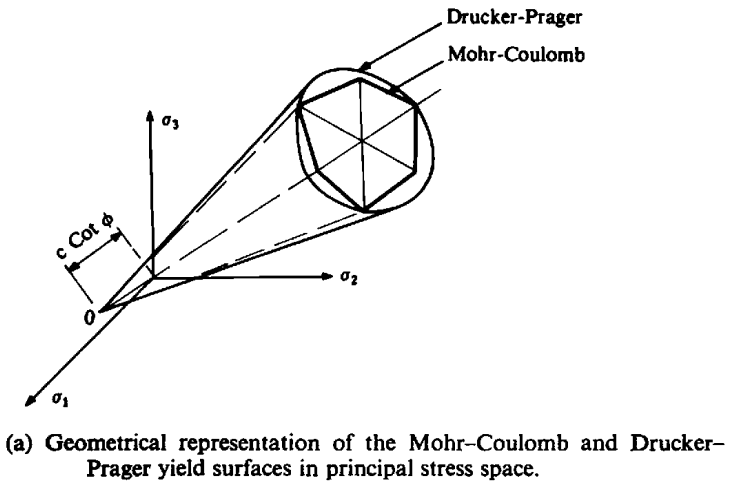
\includegraphics[width=6cm]{images/rheology/owenhinton5}\\
{\captionfont Taken from \textcite{owhi}.}
\end{center}

Using the parameters $\sigma_m$, $\tau_m$, $a=-\sqrt{3}\tan\theta$, ${\cal I}_1({\bm \sigma})$ 
and ${\cal I}_2({\bm \tau})$ of Section~\ref{sec:altinv} we have
\begin{eqnarray}
F^{\text{\tiny DP}}
&=&  \sqrt{{\cal I}_2({\bm \tau})} + \alpha {\cal I}_1({\bm \sigma}) + k \nn\\
&=& \sqrt{\frac{\tau_m^2}{3}(a^2+3)} + \alpha (3\sigma_m-a\tau_m) + k \nn\\ 
&=& \tau_m \sqrt{(a^2/3+1)} + \alpha (3\sigma_m+\tau_m\sqrt{3}\tan\theta ) + k    \qquad ({\rm since }\; \tau_m>0)\nn\\ 
&=& \tau_m \sqrt{\tan^2\theta+1} + \alpha (3\sigma_m+\tau_m\sqrt{3}\tan\theta ) + k  \nn\\
&=& \tau_m \sqrt{ \frac{1}{\cos^2\theta} } + \alpha (3\sigma_m+\tau_m\sqrt{3}\tan\theta ) + k  \nn\\
&=& \tau_m \frac{1}{\cos\theta} +\alpha (3\sigma_m+\tau_m\sqrt{3}\tan\theta ) + k  \qquad ({\rm since }\; \cos\theta >0)\nn
\end{eqnarray}
$F=0$ then leads to write
\begin{eqnarray}
\tau_m  + (3 \alpha \sigma_m+k)\cos\theta  + \tau_m \alpha \sqrt{3}\sin\theta  &=&0 \nn\\
\Rightarrow \qquad \tau_m(1 + \alpha \sqrt{3}\sin\theta)  + (3 \alpha \sigma_m+k)\cos\theta &=&0 \nn
\end{eqnarray}
and finally
\[
\tau_m = -\frac{(3 \alpha \sigma_m+k)\cos\theta}{1 + \alpha \sqrt{3}\sin\theta}
= -\frac{3 \alpha \cos\theta}{1 + \alpha \sqrt{3}\sin\theta} \sigma_m 
-\frac{k\cos\theta}{1 + \alpha \sqrt{3}\sin\theta}
\]
\begin{remark}
This is the same equation as Eq.~19 of Wojciechowski \cite{wojc18} but with $\theta \rightarrow -\theta$. 
\end{remark}

\vspace{.5cm}

The Mohr-Coulomb yield criterion writes  (see Eq.~\eqref{eq:mccrit})
\[
\tau_m = -\sigma_m \sin\phi + c \cos\phi
\]
so that equating both expressions of $\tau_m$ for the Drucker-Prager 
and Mohr-Coulomb criteria leads to:
\begin{eqnarray}
-\frac{3 \alpha \cos\theta}{1 + \alpha \sqrt{3}\sin\theta} &=& -\sin\phi \label{eq:qq1}\\
-\frac{k\cos\theta}{1 + \alpha \sqrt{3}\sin\theta} &=& c \cos\phi \label{eq:qq2}
\end{eqnarray}
Eq.~\eqref{eq:qq1} yields
\[
3 \alpha \cos\theta = \sin\phi (1 + \alpha \sqrt{3}\sin\theta) 
\]
\[
\Rightarrow \qquad 3 \alpha \cos\theta - \alpha \sqrt{3}\sin\theta \sin\phi = \sin\phi 
\]
and finally 
\[
\boxed{
\alpha(\phi) =  \frac{\sin\phi}{ 3 \cos\theta - \sqrt{3}\sin\theta \sin\phi}
}
\]
Inserting this into Eq.~\eqref{eq:qq2}:
\begin{eqnarray}
- k \cos\theta 
&=& c \cos \phi \left(1 +\alpha \sqrt{3} \sin\theta \right)  \nn\\
&=& c \cos \phi \left(1 + \frac{\sin\phi}{ 3 \cos\theta - \sqrt{3}\sin\theta \sin\phi}  \sqrt{3} \sin\theta\right) \nn\\
&=& c \cos \phi \left(1 + 
\frac{ \sqrt{3}\sin\phi \sin\theta }{ 3 \cos\theta - \sqrt{3}\sin\theta \sin\phi} \right) \nn\\
&=& c \cos \phi \left(
\frac{ 3 \cos\theta - \sqrt{3}\sin\theta \sin\phi}{ 3 \cos\theta - \sqrt{3}\sin\theta \sin\phi} 
+ 
\frac{ \sqrt{3}\sin\phi \sin\theta }{ 3 \cos\theta - \sqrt{3}\sin\theta \sin\phi} \right) \nn\\
&=& c \cos \phi \left(
\frac{ 3 \cos\theta}{ 3 \cos\theta - \sqrt{3}\sin\theta \sin\phi} \right) \nn
\end{eqnarray}
so that 
\[
\boxed{
k(c,\phi) =- \frac{ 3\; c \cos \phi }{ 3 \cos\theta - \sqrt{3}\sin\theta \sin\phi} 
}
\]
%Unsurprisingly we recover the Eqs. 20 and 21 of Wojciechowski \cite{wojc18} by replacing $\theta$ by $-\theta$.

The Drucker-Prager yield criterion which for a given $\theta$ is equal to the Mohr-Coulomb yield is then:
\begin{eqnarray}
F^{\text{\tiny DP}}
&=& \sqrt{{\cal I}_2({\bm \tau})} + \alpha(\phi) {\cal I}_1({\bm \sigma}) + k(c,\phi)  \nn\\
&=& \sqrt{{\cal I}_2({\bm \tau})} 
+ \frac{\sin\phi}{ 3 \cos\theta - \sqrt{3}\sin\theta \sin\phi}  {\cal I}_1({\bm \sigma})  
- \frac{ 3\; c \cos \phi }{ 3 \cos\theta - \sqrt{3}\sin\theta \sin\phi} \nn\\
&=& \sqrt{{\cal I}_2({\bm \tau})} 
- \left[ -\frac{3 \sin\phi}{ 3 \cos\theta - \sqrt{3}\sin\theta \sin\phi}  \frac{{\cal I}_1({\bm \sigma})}{3}
+ \frac{ 3\; c \cos \phi }{ 3 \cos\theta - \sqrt{3}\sin\theta \sin\phi} \right] \label{eq:Fdp}\\
&=& \sqrt{{\cal I}_2({\bm \tau})} 
- \left[ \frac{3\; p \sin\phi}{ 3 \cos\theta - \sqrt{3}\sin\theta \sin\phi} 
+ \frac{ 3\; c \cos \phi }{ 3 \cos\theta - \sqrt{3}\sin\theta \sin\phi} \right] \nn\\
&=& \sqrt{{\cal I}_2({\bm \tau})}  
- \frac{3\; p \sin\phi  + 3\; c \cos \phi }{ 3 \cos\theta - \sqrt{3}\sin\theta \sin\phi} \nn\\ 
&=& \sqrt{{\cal I}_2({\bm \tau})}  
- \frac{p \sin\phi  + c \cos \phi }{  \cos\theta - \frac{1}{\sqrt{3}}\sin\theta \sin\phi} 
\end{eqnarray}
which, when multiplied by $\cos\theta - \frac{1}{\sqrt{3}}\sin\theta \sin\phi$, gives
the Mohr-Coulomb criterion of Eq.~\eqref{eq:mcF}. 

For $\theta=\pi/6$, the DP yield surface {\bf circumscribes} the MC yield 
surface and Eq.~\eqref{eq:Fdp} writes:
\begin{eqnarray}
F^{\text{\tiny DP}}
&=& \sqrt{{\cal I}_2({\bm \tau})} 
- \left[ -\frac{3 \sin\phi}{ 3 \sqrt{3}/2 - \sqrt{3}/2 \; \sin\phi}  \frac{{\cal I}_1({\bm \sigma})}{3}
+ \frac{ 3\; c \cos \phi }{ 3 \sqrt{3}/2 - \sqrt{3}/2 \; \sin\phi} \right] \nn\\
&=& \sqrt{{\cal I}_2({\bm \tau})} 
- \left[ -\frac{6 \sin\phi}{\sqrt{3} (3 - \sin\phi) }  \frac{{\cal I}_1({\bm \sigma})}{3}
+ \frac{ 6\; c \cos \phi }{ \sqrt{3}(3 - \sin\phi)} \right] \nn\\
&=& \sqrt{{\cal I}_2({\bm \tau})} 
- \frac{ 6 p \sin \phi + 6\; c \cos \phi }{ \sqrt{3}(3 - \sin\phi)} \label{eq:dpc}
\end{eqnarray}
i.e.

\begin{center}
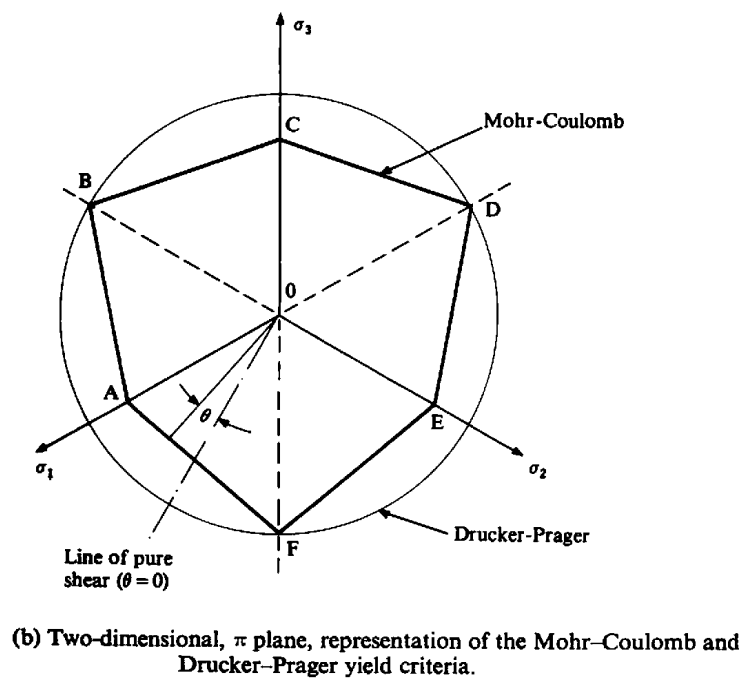
\includegraphics[width=5cm]{images/rheology/owenhinton6}\\
{\captionfont Taken from \textcite{owhi}.}
\end{center}

\begin{mdframed}[backgroundcolor=blue!5]
\begin{equation}
F^{\text{\tiny DP}}
= \sqrt{{\cal I}_2({\bm \tau})} 
+ \frac{ 6 \sin \phi }{ \sqrt{3}(3 - \sin\phi)} \frac{{\cal I}_1({\bm\sigma})}{3}
- \frac{ 6\; c \cos \phi }{ \sqrt{3}(3 - \sin\phi)} 
\end{equation}
\end{mdframed}

which is the formula used in Glerum \etal (2018) \cite{gltf18}.
This is also Eq.~(14a) in Zienkiewicz \& Cormeau (1974) \cite{zico74}, 
Eq.~(7.18) in \textcite{owhi}, and Eq.~(13.10a) in Zienkiewicz (1975) \cite{zien75} 
provided it is divided altogether by $\sqrt 3$. 


For $\theta=-\pi/6$, the DP yield surface {\bf middle circumscribes} the MC yield surface 
and Eq.~\eqref{eq:Fdp} writes:
\begin{eqnarray}
F^{\text{\tiny DP}}
&=& \sqrt{{\cal I}_2({\bm \tau})} 
- \left[ -\frac{3 \sin\phi}{ 3 \sqrt{3}/2 + \sqrt{3}/2 \sin\phi}  \frac{{\cal I}_1({\bm \sigma})}{3}
+ \frac{ 3\; c \cos \phi }{ 3 \sqrt{3}/2 + \sqrt{3}/2 \sin\phi} \right] \nn\\
&=& \sqrt{{\cal I}_2({\bm \tau})} 
- \left[ -\frac{6 \sin\phi}{\sqrt{3} (3 + \sin\phi) }  \frac{{\cal I}_1({\bm \sigma})}{3}
+ \frac{ 6\; c \cos \phi }{ \sqrt{3}(3 + \sin\phi}) \right] \nn\\
&=& \sqrt{{\cal I}_2({\bm \tau})} 
- \frac{6 p \sin\phi + 6 c \cos \phi}{\sqrt{3} (3 + \sin\phi) } 
\end{eqnarray}
This is Eq.~(7.19) of \textcite{owhi}.

Another DP formulation which {\bf inscribes} the MC yield surface is found on the 
wikipedia page of the Drucker-Prager yield criterion
\footnote{\url{https://en.wikipedia.org/wiki/Drucker-Prager_yield_criterion}}
(but I have no idea how it is arrived at):
\begin{eqnarray}
F^{\text{\tiny DP}}
&=& \sqrt{{\cal I}_2({\bm \tau})} 
- \left[ -\frac{3 \sin\phi}{\sqrt{9+3\sin^2\phi} }  \frac{{\cal I}_1({\bm \sigma})}{3}
+ \frac{ 3\; c \cos \phi }{ \sqrt{9+3\sin^2\phi} } \right] \label{eq:dp3}
\end{eqnarray}

The yield surfaces of these three Drucker-Prager formulations are plotted against the Mohr-Coulomb
yield surface in Section~\ref{ss:envelope}. 



%%%%%%%%%%%%%%%%%%%%%%%%%%%%%%%%%%
%\paragraph{two-dimensional space}

%By choosing $k=c \cos \phi $ and $\alpha=\frac{1}{2}\sin \phi$ and seeing that that $p=\frac{1}{2} {\cal I}_1({\bm \sigma})$, we can make the Drucker-Prager yield criterion coincide with the Mohr-Coulomb yield criterion
%so that 
%\begin{equation}
%F^{DP,2D} = \tau_e - (p \sin \phi + c \; \cos \phi) 
%\end{equation}


%%%%%%%%%%%%%%%%%%%%%%%%%%%%%%%%%%
%\paragraph{three-dimensional space}

%Let us first assume that the Drucker-Prager yield surface circumscribes the Mohr-Coulomb yield surface such that the two surfaces coincide at $\theta=\tfrac{\pi}{3}$. 
%The expression for the Mohr-Coulomb yield criterion is

%\[
%F^{MC,3D} = -\frac{1}{3}J_1 \sin \phi  + \sqrt{J_2} ( \cos \theta - \frac{1}{\sqrt{3}} \sin \theta  \sin \phi ) - c \cos \phi 
%\]
%Taking $\theta=\pi/6$ yields:
%\begin{eqnarray}
%F^{MC,3D} 
%&=& -\frac{1}{3}J_1 \sin \phi  + \sqrt{J_2} ( \frac{\sqrt{3}}{2} - \frac{1}{\sqrt{3}} \frac{1}{2}  \sin \phi ) - c \cos \phi  \nn\\
%&=& -\frac{1}{3}J_1 \sin \phi  + \frac{1}{2\sqrt{3}}\sqrt{J_2} ( 3 -  \sin \phi ) - c \cos \phi  \nn\\
%&=& -\frac{1}{3}J_1 \sin \phi  + \frac{1}{6}\sqrt{J_2} \sqrt{3}( 3 -  \sin \phi ) - c \cos \phi  \nn\\
%&=& \frac{\sqrt{3}(3-\sin\phi)}{6} \left( -  \frac{2 \sin \phi}{\sqrt{3}(3-\sin\phi)}   J_1  + \sqrt{J_2}  - \frac{6c \cos \phi}{\sqrt{3}(3-\sin\phi)} \right) \nn
%\end{eqnarray}
%The constant in front of the brackets (which always strictly positive) does not matter since we look at the sign of $F$.
%Comparing with 
%\[
%F^{DP}=\sqrt{J_2} - (\alpha J_1 + k) \label{dpcriterion} 
%\]
%we naturally set 
%\[
%\alpha =\frac{2 \sin \phi}{\sqrt{3}(3-\sin\phi)}
%\quad\quad\quad  
%k =  \frac{6c \cos \phi}{\sqrt{3}(3-\sin\phi)} 
%\]
%and since $p=\frac{1}{3}{\cal I}_1({\bm \sigma})$:
%\begin{mdframed}[backgroundcolor=blue!5]
%\begin{equation}
%F^{DP,3D} = \tau_e  - \left[ \frac{6 \sin \phi}{\sqrt{3}(3-\sin\phi)}   p  + 
%\frac{6c \cos \phi}{\sqrt{3}(3-\sin\phi)}  \right]
%\label{eqdp3D}
%\end{equation}
%\end{mdframed}
%\begin{center}
%\includegraphics[width=0.6\textwidth]{RHEOLOGY/viscoplasticity/dpcriterion.pdf}
%\end{center}


\vspace{1.3cm}
%..............
\begin{remark}
Leroy \& Ortiz \cite{leor89} use the Drucker-Prager plasticity model also and match it to the Mohr-Coulomb model in the 
triaxial test and formulate it as follows 
(Their definition of the second invariant of stress contains a 3/2 term):
\begin{eqnarray}
F 
&=& \tau_e \sqrt{3} + \frac{6 \sin\phi}{3-\sin\phi} \left( -p  - \frac{c}{\tan \phi} \right) \nn\\
&=& \tau_e \sqrt{3} - \left( \frac{6 \sin\phi}{3-\sin\phi}  p  + c \frac{6 \cos\phi}{3-\sin\phi} \right) \nn\\
&=& \sqrt{3} \left[ \tau_e  - \left( \frac{6 \sin\phi}{\sqrt{3}(3-\sin\phi)}  p  + c \frac{6 \cos\phi}{\sqrt{3}(3-\sin\phi)} \right)  \right]
\end{eqnarray}
Except for the $\sqrt{3}$ this is identical to Eq.~\eqref{eq:dpc}.
\end{remark}

%..............
\begin{remark}
Bui \etal (2008) \cite{bufs08} use yet again another formulation:
\begin{eqnarray}
F 
&=& \sqrt{{\cal I}_2({\bm \tau})} + \frac{\tan \phi}{\sqrt{9 + 12 \tan^2 \phi}} {\cal I}_1({\bm \sigma})
- \frac{3 c}{\sqrt{9 + 12 \tan^2 \phi}} \nn\\
&=& \sqrt{{\cal I}_2({\bm \tau})} + \frac{\sin \phi}{\sqrt{9\cos^2 \phi + 12 \sin^2 \phi}} {\cal I}_1({\bm \sigma}) - \frac{3 c \; \cos\phi}{\sqrt{9\cos^2\phi + 12 \sin^2 \phi}} \nn\\
&=& \sqrt{{\cal I}_2({\bm \tau})} + \frac{\sin \phi}{\sqrt{9 + 3 \sin^2 \phi}} {\cal I}_1({\bm \sigma}) - \frac{3 c \; \cos\phi}{\sqrt{9 + 3\sin^2 \phi}} \nn
\end{eqnarray}
which is identical to \eqref{eq:dp3}.
\end{remark}

%..............
\begin{remark}
Cacace \& Jacquey (2017) \cite{caja17} replace $\sqrt{{\cal I}_2({\bm \tau})}$ by 
$\sqrt{{\cal I}_2({\bm \tau})+\epsilon_0^2}$ where $\epsilon_0$ is a small non-hardening parameters 
here introduced to relax the singularity at the cone's tip of the Drucker-Prager yield envelope.
\end{remark}

\Literature:
\fullcite{cuwi14}


%.............................................................................
\paragraph{Dissecting the original paper by Drucker and Prager (1952)}


The authors state that a yield function which is a proper generalisation of the M-C hypothesis is:
\[
F = \alpha {\cal I}_1(\bm\sigma) + \sqrt{{\cal I}_2(\bm\tau)} - k
\]
where $\alpha$ and $k$ are positive constants at each point of the material.

According to the concept of plastic potential, the stress-train relation
corresponding to this yield function is 
\[
\dot\varepsilon_{ij}^{p} = \lambda \frac{\partial F}{\partial \sigma_{ij}}
\]
where $\dot\varepsilon_{ij}^{p}$ is the plastic strain rate and $\lambda$
is a positive factor of proportionality which may assume different values in space. Using the above expression for $F$:
\begin{equation}
\dot\varepsilon_{ij}^{p} = \lambda \left( \alpha \delta_{ij} + \frac{\tau_{ij}}{2\sqrt{{\cal I}_2(\bm\tau)}} \right)
\label{eq:dp52:ab}
\end{equation}
A very important feature of this equation is that the plastic rate of cubical
dilation is 
\begin{equation}
{\rm tr}[\dot{\bm \varepsilon}^{p}]
=\dot\varepsilon_{ii}^{p} = 3 \alpha \lambda \ne 0
\label{eq:dp52:bc}
\end{equation}
This equation shows that plastic deformation must be accompanied by an increase
in volume if $\alpha\ne 0$. This property is known as dilatancy.

%-----------------------------------------------------------------------
\paragraph{Plane strain} 
We need to establish three expressions.  
First, from Eq.~\eqref{eq:dp52:ab} we can write 
\[
\dot\varepsilon_{zz}^{p} = \lambda \left( \alpha  + \frac{\tau_{zz}}{2\sqrt{{\cal I}_2(\bm\tau)}} \right)
\]
but since $\dot\varepsilon_{zz}=0$ in plane strain then we find
\begin{equation}
\tau_{zz} = - 2 \alpha \sqrt{{\cal I}_2(\bm\tau)}
\end{equation}
which is Eq.~(6) of the paper. 

Second, we start from the definition of the first invariant and use the equation above:
\begin{eqnarray}
{\cal I}_1(\bm \sigma)&=& \sigma_{xx}+\sigma_{yy}+\sigma_{zz} \nn\\
{\cal I}_1(\bm \sigma)&=& \sigma_{xx}+\sigma_{yy}+\tau_{zz}+\frac13 {\cal I}_1(\bm \sigma) \nn\\
{\cal I}_1(\bm \sigma)&=& \sigma_{xx}+\sigma_{yy}- 2 \alpha \sqrt{{\cal I}_2(\bm\tau)} 
+\frac13 {\cal I}_1(\bm \sigma)\nn\\
\frac23 {\cal I}_1(\bm \sigma)&=& \sigma_{xx}+\sigma_{yy}- 2 \alpha \sqrt{{\cal I}_2(\bm\tau)} \nn\\
{\cal I}_1(\bm \sigma)&=& \frac32(\sigma_{xx}+\sigma_{yy})- 3 \alpha \sqrt{{\cal I}_2(\bm\tau)} 
\label{eq:I1dpps}
\end{eqnarray}
which is Eq.~(7) of the paper.

Finally, we start from (and we use the fact that $\sigma_{xx}-\sigma_{yy}=\tau_{xx}-\tau_{yy}$)
\begin{eqnarray}
\left(\frac{\sigma_{xx}-\sigma_{yy}}{2} \right)^2 + \tau_{xy}^2
&=& \frac14 \left(\sigma_{xx}-\sigma_{yy} \right)^2 + \tau_{xy}^2 \nn\\
&=& \frac14 \left(\sigma_{xx}-\sigma_{yy} \right)^2 
+ \underbrace{\tau_{xy}^2 
+ \frac12 (\tau_{xx}^2+\tau_{yy}^2+\tau_{zz}^2)}_{{\cal I}_2(\bm\tau)}
- \frac12 (\tau_{xx}^2+\tau_{yy}^2+\tau_{zz}^2) \nn\\
&=& \frac14 \left(\tau_{xx}-\tau_{yy} \right)^2 
+ {\cal I}_2(\bm\tau)
- \frac12 \tau_{xx}^2 -\frac12 \tau_{yy}^2 -\frac12 \tau_{zz}^2 \nn\\
&=& {\cal I}_2(\bm\tau) +\frac14\tau_{xx}^2 -\frac12\tau_{xx}\tau_{yy} +\frac14\tau_{yy}^2
- \frac12 \tau_{xx}^2 -\frac12\tau_{yy}^2 -\frac12 4\alpha^2 {\cal I}_2(\bm\tau) \nn\\
&=& {\cal I}_2(\bm\tau) -\frac14\tau_{xx}^2 -\frac12\tau_{xx}\tau_{yy} -\frac14\tau_{yy}^2
-2\alpha^2 {\cal I}_2(\bm\tau) \nn\\
&=& {\cal I}_2(\bm\tau) -\frac14(\tau_{xx}^2 +2\tau_{xx}\tau_{yy} +\tau_{yy}^2)
-2\alpha^2 {\cal I}_2(\bm\tau) \nn\\
&=& {\cal I}_2(\bm\tau) -\frac14(\underbrace{\tau_{xx}+\tau_{yy}}_{-\tau_{zz}})^2
-2\alpha^2 {\cal I}_2(\bm\tau) \nn\\
&=& {\cal I}_2(\bm\tau) -\frac14 \tau_{zz}^2 -2\alpha^2 {\cal I}_2(\bm\tau) \nn\\
&=& {\cal I}_2(\bm\tau) -\frac14 4\alpha^2 {\cal I}_2(\bm\tau) -2\alpha^2 {\cal I}_2(\bm\tau) \nn\\
&=& {\cal I}_2(\bm\tau) -3\alpha^2 {\cal I}_2(\bm\tau) \nn\\
&=& {\cal I}_2(\bm\tau)(1 -3\alpha^2)
\end{eqnarray}
so that 
\begin{equation}
{\cal I}_2(\bm\tau) = \frac{1}{1 -3\alpha^2} \left[\left(\frac{\sigma_{xx}-\sigma_{yy}}{2} \right)^2 + \tau_{xy}^2 \right]
\label{eq:dp52:cd}
\end{equation}
which is Eq.~(8) of the paper.

In the paper the authors propose the yield function 
\[
F = \alpha {\cal I}_1(\bm\sigma) + \sqrt{{\cal I}_2(\bm\tau)} - k
\]
We first replace the first (plane strain) invariant (see Eq.~\eqref{eq:I1dpps}):
\begin{eqnarray}
F 
&=& \alpha \left[ \frac32(\sigma_{xx}+\sigma_{yy})- 3 \alpha \sqrt{{\cal I}_2(\bm\tau)} \right]
+ \sqrt{{\cal I}_2(\bm\tau)} - k \nn\\
&=&\alpha \frac32(\sigma_{xx}+\sigma_{yy})- 3 \alpha^2 \sqrt{{\cal I}_2(\bm\tau)}
+ \sqrt{{\cal I}_2(\bm\tau)} - k  \nn\\
&=&\alpha \frac32(\sigma_{xx}+\sigma_{yy}) +(1- 3 \alpha^2) \sqrt{{\cal I}_2(\bm\tau)} - k \nn
\end{eqnarray}
and we now introduce the second invariant of Eq.~\eqref{eq:dp52:cd}:
\begin{eqnarray}
F &=& 
\alpha \frac32(\sigma_{xx}+\sigma_{yy}) +(1- 3 \alpha^2)
\frac{1}{(1 -3\alpha^2)^{1/2}} \left[\left(\frac{\sigma_{xx}-\sigma_{yy}}{2} \right)^2 
+ \tau_{xy}^2 \right]^{1/2} -  k  \nn\\
&=& \alpha \frac32(\sigma_{xx}+\sigma_{yy}) +(1- 3 \alpha^2)^{1/2}
\left[\left(\frac{\sigma_{xx}-\sigma_{yy}}{2} \right)^2 + \tau_{xy}^2 \right]^{1/2} 
- k  \nn\\
&=&\frac{3\alpha}{(1- 3 \alpha^2)^{1/2}}
\frac12(\sigma_{xx}+\sigma_{yy}) +
\left[\left(\frac{\sigma_{xx}-\sigma_{yy}}{2} \right)^2 + \tau_{xy}^2 \right]^{1/2} 
- \frac{k}{(1- 3 \alpha^2)^{1/2}} 
\nn\\
&=&\underbrace{\frac{3\alpha}{(1- 3 \alpha^2)^{1/2}}}_{\sin\phi}
\frac12(\sigma_{xx}+\sigma_{yy}) +
\left[\left(\frac{\sigma_{xx}-\sigma_{yy}}{2} \right)^2 + \tau_{xy}^2 \right]^{1/2} 
- \underbrace{\frac{k}{(1- 12 \alpha^2)^{1/2}}}_{c}
\underbrace{\frac{(1- 12 \alpha^2)^{1/2}}{(1- 3 \alpha^2)^{1/2}}}_{\cos\phi}
\end{eqnarray}


Note that if we define a triangle with sides $(1- 12 \alpha^2)^{1/2}$ and $3\alpha$
with hypotenuse $(1- 3 \alpha^2)^{1/2}$ then the angle $\phi$ makes sense and
we recover $\cos^2\phi+\sin^2\phi=1$.

In the end:
\[
F = 
\left[\left(\frac{\sigma_{xx}-\sigma_{yy}}{2} \right)^2 + \tau_{xy}^2 \right]^{1/2}
-\left(-\frac12(\sigma_{xx}+\sigma_{yy}) \sin \phi + c \cos \phi \right)
\]
which is the Mohr-Coulomb yield criterion of Eq.~(1) in the paper.


Note that when $\alpha=0$ (yield criterion independent of the mean stress - incompressible flow see Eq.~\eqref{eq:dp52:bc}) then $c=k$, $\cos\phi=1$ and $\sin\phi=0$ and we find 
the Tresca yield criterion
\[
F^{TR}=  \left[\left(\frac{\sigma_{xx}-\sigma_{yy}}{2} \right)^2 + \tau_{xy}^2 \right]^{1/2} - k
\]
Also, setting $\alpha=0$ in Eq.~\eqref{eq:dp52:cd} yields a criterion that writes
\[
F^{vM}={\cal I}_2(\bm\tau) - k
\]
which is the von Mises criterion! 



\vspace{.5cm}

We now look into the derivatives of the Drucker-Prager plastic potential $Q^{\text{\tiny DP}}(\bm\sigma)$.
We have
\[
Q^{\text{\tiny DP}} (\bm\sigma)= \sqrt{{\cal I}_2({\bm \tau})} + \alpha {\cal I}_1({\bm \sigma}) + k 
\]
Then
\begin{eqnarray}
\frac{\partial Q^{\text{\tiny DP}} }{\partial {\cal I}_1(\bm\sigma)} &=& \alpha \\
\frac{\partial Q^{\text{\tiny DP}} }{\partial \sqrt{{\cal I}_2(\bm\tau)}}&=& 1  \\
\frac{\partial Q^{\text{\tiny DP}} }{\partial \theta_{\rm L}(\bm\tau)} &=& 0 
\end{eqnarray}
The parameters $\alpha$ and $k$ can be expressed as a function of the angle of friction 
and cohesion so as to match the Mohr-Coulomb criterion in some sense (see above).
Then
\begin{eqnarray}
C_1^{\text{\tiny DP}} &=& \alpha  \\ 
C_2^{\text{\tiny DP}} &=& \frac{1}{2  \sqrt{{\cal I}_2(\bm\tau)}   }  \\ 
C_3^{\text{\tiny DP}} &=& 0  
\end{eqnarray}

ToDo: check \textcite{albo12} (2012) and compare with my notes above.









\newpage


%------------------------------
\subsubsection{The Griffith-Murrell failure criterion}
\index{general}{Griffith-Murrell}

The Griffith-Murrell yield criterion \cite{brau94,brbe95,babr97} is not often used. 
Extending the work of Griffith (1921) to three dimensional stress distributions, 
Murrell (1963) suggested the following criterion for rock failure expressed 
in terms of the principal stresses:
\[
(\sigma_1-\sigma_2)^2 + (\sigma_2-\sigma_3)^2 + (\sigma_3-\sigma_1)^2
+
24T_0 (\sigma_1+\sigma_2+\sigma_3)=0
\]
where $T_0$ is a material property called the tensile strength. In principal stress space, 
this criterion is represented by a paraboloid of revolution around the pressure (or hydrostatic) axis.

Using the definition of ${\cal I}_2({\bm \tau})$ and ${\cal I}_1({\bm \sigma})$, it also writes:
\[
{\cal I}_2({\bm \tau}) - 12 T_0 p =0
\]
which is the formulation used in Hansen \etal (2000) \cite{hanl00}, although the authors
use the lithostatic pressure instead of the full pressure. They also use a tensile 
strength parameter $T_0^e$ and a compressive strength parameter $T_0^c$, both around a few tens 
of MPas.

%------------------------------
\subsubsection{The Cam-clay failure criterion}
\index{general}{Cam-clay Failure Criterion}

\begin{flushright} {\tiny {\color{gray} camclay.tex}} \end{flushright}
%~~~~~~~~~~~~~~~~~~~~~~~~~~~~~~~~~~~~~~~~~~~~~~~~~~~~~~~~~~~~~~~~~~~~~~~~~~~~~~~~~~~~~~~~~~~~~~~~~~

The Original Cam-Clay model is based on the assumption that the soil 
is isotropic, elasto-plastic, deforms as a continuum, and it is not affected by creep.

\Literature: \cite{pehu03}

\todo[inline]{ask Chris Spiers. Pijnenburg et al, JGR 2019}


%.........................................................
\subsubsection{The failure envelope, or yield surface}
\label{ss:envelope} 

\Literature: Sch{\"o}pfer \etal (2013) \cite{sccm13}.

A yield surface is a five-dimensional surface in the six-dimensional space of stresses. 
The state of stress of inside the yield surface is elastic. 
When the stress state lies on the surface the material is said to have reached its yield point 
and the material is said to have become plastic. Further deformation of the material causes 
the stress state to remain on the yield surface, even though the surface itself may change shape and 
size as the plastic deformation evolves, this is because stress states that lie outside the yield surface are non-permissible.

The yield surface is usually expressed in terms of (and visualized in) a three-dimensional principal stress space $(\sigma_1,\sigma_2,\sigma_3)$, a two- or three-dimensional space spanned by stress invariants 
or a version of the three-dimensional Haigh-Westergaard space. 

\begin{center}
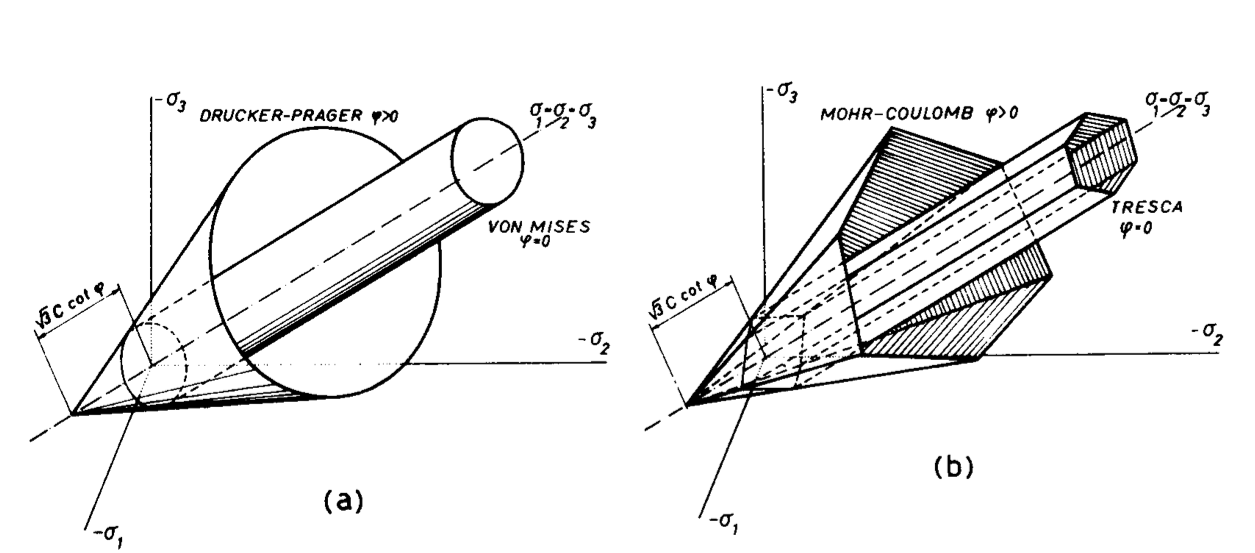
\includegraphics[width=14cm]{images/rheology/surfaces}\\
{\captionfont Yield surfaces in stress space \cite{zico74}. Note that 
the axes are $-\sigma_1$,$-\sigma_2$,$-\sigma_3$}
\end{center} 

Having obtained the equations for the yield functions in the previous sections, we can easily test
them as follows: in the ($\sigma_1$, $\sigma_2$, $\sigma_3$) space we can look for stress states 
that fulfil the yield equations. I set $c=20$MPa and $\phi=20$\degree and restrain 
the search to the space [-100MPa:100MPa]$^3$.
The python code and the gnuplot script used to generate the plots hereafter 
are in {\tt images/rheology/surfaces}. The implemented algorithm is somewhat  
naive and quite inefficient: discretise the space in $N^3$ points and for each point 
check whether any of the von Mises, Tresca, Mohr-Coulomb and (the three variants of) Drucker-Prager 
criteria is satisfied and when the point is in the space $\sigma_1+\sigma_2+\sigma_3=10$MPa 
(perpendicular to the $x=y=z$ line) write it to the corresponding file.

The recovered surfaces are similar to those of the figure above but their plot in a 3D space is difficult.
I have therefore isolated two sub-plots. 
The first one is for $\sigma_1=\sigma_2$:

\begin{center}
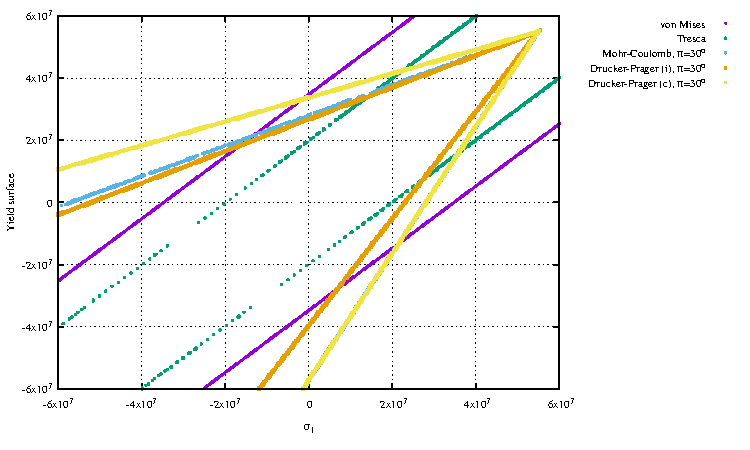
\includegraphics[width=12cm]{images/rheology/surfaces/surfaces_xy.pdf}
\end{center}
We see that the von Mises and Tresca envelopes are parallel to the line $\sigma_1=\sigma_2=\sigma_3$ (which 
is expected since they do not depend on pressure).

The second plot is in the plane $\sigma_1+\sigma_2+\sigma_3=0$ which is perpendicular to the middle line 
$\sigma_1=\sigma_2=\sigma_3=0$. To facilitate plotting the envelopes are plotted as a function of $\sigma_1$ only (so that even though they are circles in the chosen plane they appear here as ellipses):

\begin{center}
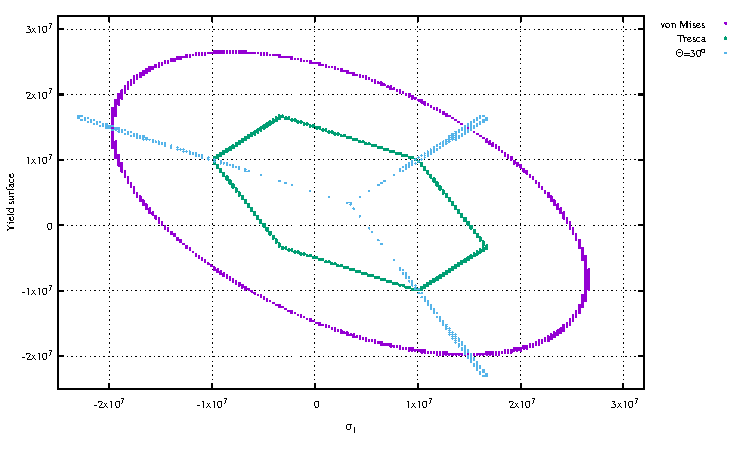
\includegraphics[width=12cm]{images/rheology/surfaces/surfaces_plane2.pdf}
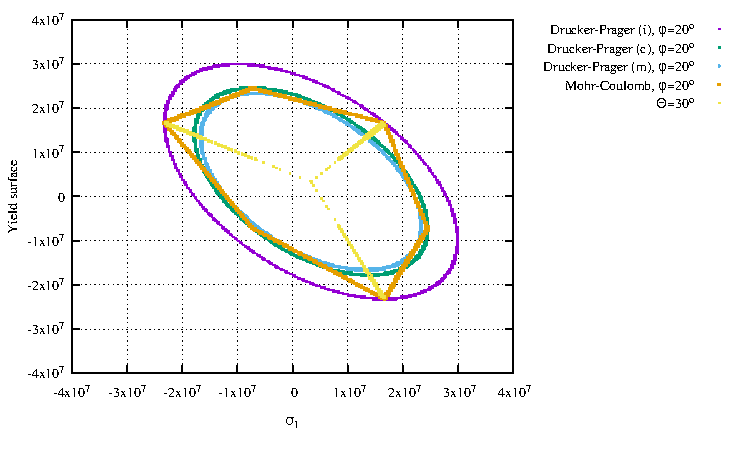
\includegraphics[width=12cm]{images/rheology/surfaces/surfaces_plane.pdf}
\end{center}

We see that we indeed recover that the three Drucker-Prager formulations 
inscribe (purple), middle-circumscribe (blue) and circumscribe (green) the 
Mohr-Coulomb one. 



\newpage
%------------------------------
\subsubsection{Peierls creep}
\index{general}{Peierls creep}

Looking at the literature, there seem to be many formulations for the Peierls creep deformation
mechanism, but it it appears that a standard formulation for the Peierls creep writes:
\[
\dot{\varepsilon} = A \sigma^n \exp \left[ -\frac{Q+pV}{RT} \left(1-(\frac{\sigma}{\sigma_P})^k\right)^q  \right]
\]
and it seems common to take $k=1$, and $n=2$ \cite{gery10,kaka08}
\[
\dot{\varepsilon} = A \sigma^2 \exp \left[ -\frac{Q+pV}{RT} \left(1-\frac{\sigma}{\sigma_P}\right)^q  \right]
\]
Elbeshausen \& Melosh (2018) \cite{elme18} use 
\[
\dot{\varepsilon} = A  \exp \left[ -\frac{Q}{RT} \left(1-\frac{\sigma}{\sigma_P}\right)^q  \right]
\]

In Chenin \etal (2019) \cite{chmd19} the authors state that their Peierls creep implementation
relies on parameters from Evans and Goetze (1979) \cite{evgo79} using the approach of 
Kameyama \etal (1999) \cite{kayk99}:
\[
\eta^{pe}=\frac{2}{3} \frac{(1-s)/s}{(1+s)/2s} A \; (\varepsilon_e^{ds})^{\frac{1}{n}-1} 
\]
with $A$ for this formulation:
\[
A = \left[ A_p \exp \left( -\frac{Q(1-\gamma)^2}{RT} \right)  \right]^{-1/s} \gamma \sigma_p
\]
where $s$ is an effective stress exponent that depends on the temperature:
\[
s = 2 \gamma \frac{Q}{RT} (1-\gamma)
\]
where $\gamma$ is a fitting parameter. 


\Literature \cite{basv06,buro11,faff11,gagd14,gery10,goev79,kaka08,kako09,kary01,mesk10,zhwa13,chsm18,shwl17}
Review article from 1966: Guyot \& Dorn \cite{gudo67}


%-------------------------------------------------
\subsubsection{Stress limiting rheology}

Taken from van Hunen \etal (2002) \cite{vavv02}:
\[
\eta_y = \tau_y \dot{\varepsilon}_y^{-1/n_y} \dot{\varepsilon}_e^{(1/n_y) -1 } 
\]
where the yield stress $\tau_y$, the yield strain rate $\dot{\varepsilon}_y$ and the yield exponent $n_y$ are
prescribed parameters. In this article, $n_y=10$, $\dot{\varepsilon}_y=10^{-15}\si{\per\second}$
When $n_y=1$ the viscosity is constant and given by $\eta_{eff} = \tau_y / \dot{\epsilon}_y$.

This rheology has also been coined pseudo-plastic in Zhong \etal (1998) \cite{zhgm98}. 
Their equation is simply  
\[
\eta_{eff} = A^{1/n} \dot{\varepsilon}_e^{-1+1/n}
\]
where $A$ is the preexponent which depends on temperature, pressure, and composition.
\begin{center}
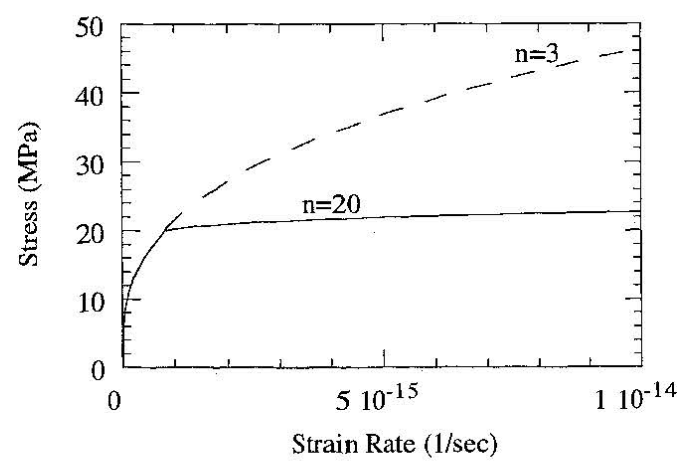
\includegraphics[width=5.5cm]{images/rheology/zhgm98}
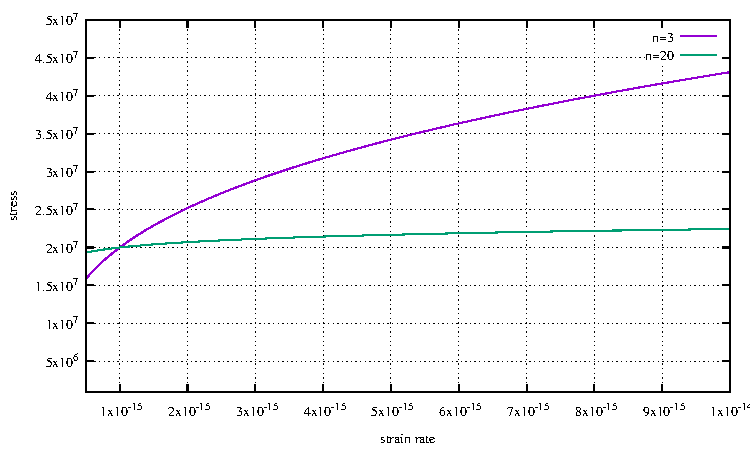
\includegraphics[width=5.8cm]{images/rheology/pseudoplastic/stress}
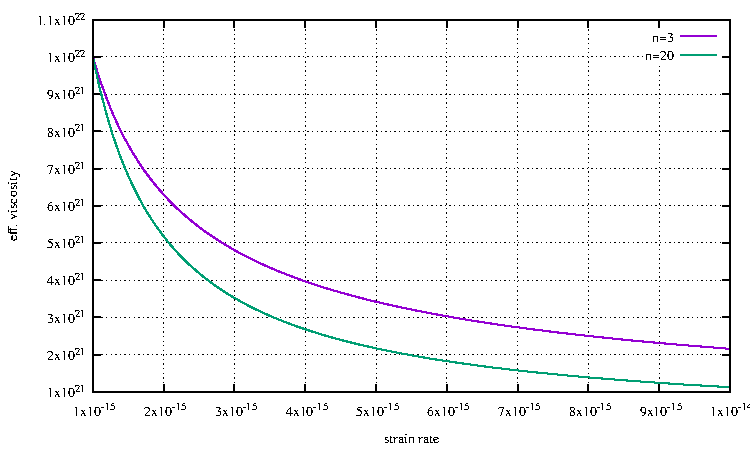
\includegraphics[width=5.8cm]{images/rheology/pseudoplastic/eta_eff}\\
{\captionfont Left figure is taken from \cite{zhgm98}. Authors report $A=7.9\cdot 10^{-8} \si{\pascal^3\second}$ 
for the $n=3$ case, which makes no sense. See gnuplot script for actual values of $A$.}
\end{center}




%-------------------------------------------------
\subsubsection{Arrhenius law}
\index{general}{Arrhenius law}

A purely temperature-dependent dimensional Arrhenius law that emulates the temperature
dependence of viscosity in silicate rock is often employed for mantle rocks 
\cite{albe00,zhzm09,vata11,bogs13b,namu13,stha13,boba19,gult19}:
\begin{equation}
\eta(T)=\eta_0 \exp \left( \frac{Q}{R}(\frac{1}{T}-\frac{1}{T_0}) \right)
\qquad 
{\rm or}
\qquad 
\eta(T)=\eta_0 \exp \left( \frac{Q}{RT} \right)
\end{equation}
where $\eta_0$ is a reference viscosity and $T_0$ its corresponding reference 
temperature.

It can also account for pressure effects as in \cite{lorg18} where the
diffusion creep viscosity (under the assumption of homogeneous grain size)
is temperature- and pressure-dependent:
\[
\eta(T)=\eta_0 \exp \left( \frac{1}{R}(\frac{Q-pV}{T}-\frac{Q}{T_0}) \right)
\]
(I find the minus sign rather suspicious)



%-------------------------------------------------
\subsubsection{Simple parametrisation of the mantle}

Many CITCOMs-based publications \cite{bumb10,budt14} 
have used the following (dimensionless) viscosity for the mantle:
\[
\eta(T,z) = \eta_r(r) \exp(A(0.5-T))
\]
where $\eta_r$ is a depth-dependent viscosity profile (usually defined as 
discontinuous linear profiles for various shells)

The non-dimensional activation coefficient is chosen to be $A=9.2103$ in 
\cite{budt14} which leads to a temperature-induced viscosity contrast of $10^4$ (for 
$T\in[0,1]$).

This is also called the Frank-Kamenetskii flow rule, as used in \cite{stha13,lemh17}:
\[
\eta' = \eta_0 \exp(-\theta T)
\]
where the the parameters $\eta_0$, $\theta$ account for the local chemical composition of the rock.
Note that the Frank-Kamenetskii approximation takes many forms in the literature \cite{nobr13}.
\index{general}{Frank-Kamenetskii}

Another temperature-dependent common expression is as follows \cite{flyu84}:
\[
\eta(T)=\eta_\infty \exp \left( \frac{Q}{R}(\frac{1}{T}-\frac{1}{T_\infty} ) \right)
\]
Also, following \cite{flyu84}: For studying transient convection in a non-
Newtonian rheological fluid, it is expedient from a
computational point of view to employ a law
which behaves linearly for low stresses initially
and becomes gradually non-Newtonian only after
a certain threshold stress level has been surpassed \cite{chri84,chyu84}:
\[
\eta(T,p,\tau_2) =\eta(T,p) \frac{1}{A_2 + A_3 \tau_2^2}
\]
where $A_2$ is a parameter describing the linear creep
at low stress levels and $A_3$ governs the transition
stress between Newtonian and non-Newtonian rheologies.

Coltice and Sheppard (2018) \cite{cosh18} use a depth- and temperature-dependent 
viscosity formulation:
\[
\eta(z,T)=\eta_0(z) \exp \frac{Q}{RT}
\]
Note that this expression is supplemented with a pseudo-plastic formulation \cite{roct12}.

\Literature: \cite{king16}

%-------------------------------------------------
\subsubsection{Glen's law for ice}\label{ss:glen}

As it turns out, ice and rocks share similarities in terms of rheology.
Glen’s law is the most commonly used flow law for ice in glaciers and ice sheets \cite{glen55}
and it is actually a power-law type rheology:
\[
\dot{\bm \varepsilon} = A {\bm \tau}^n 
\]
with $n\sim 3$ and $A\sim 2.4\cdot 10^{-24} \text{Pa}^{-3}\cdot \text{s}^{-1}$ at $0\degree$C.
The effective viscosity is then given by
\[
\eta = \frac{1}{2 A \tau_e^{n-1}} 
\]
\begin{center}
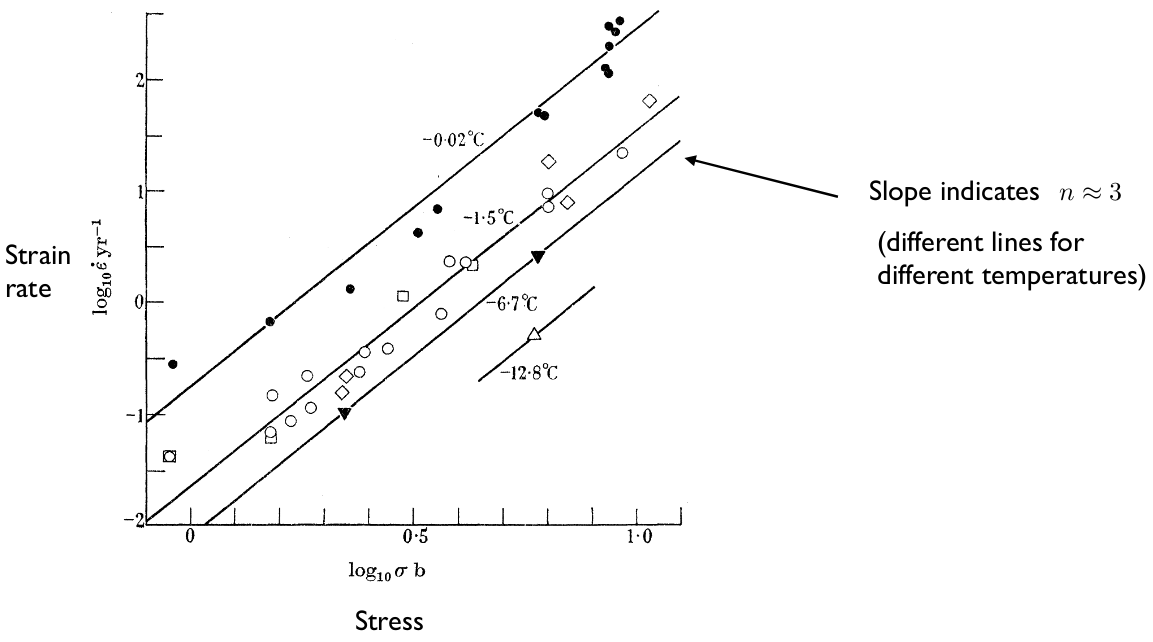
\includegraphics[height=5cm]{images/rheology/glen}
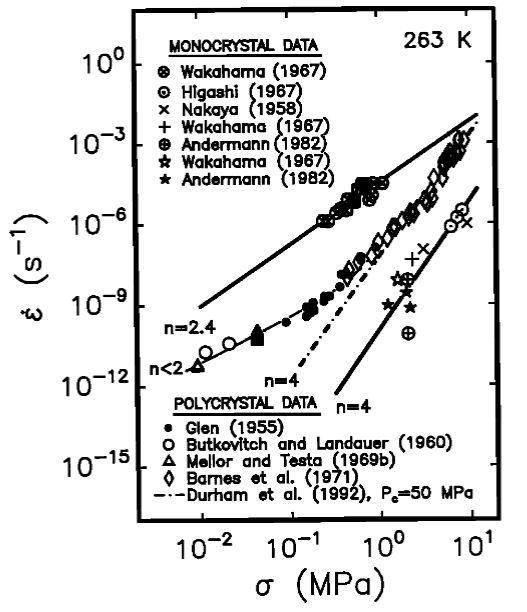
\includegraphics[height=5cm]{images/rheology/goko01}\\
{\captionfont Left: Taken from Glen \cite{glen55}; Right: taken from \cite{goko01}.}
\end{center}
Most of these studies suggest values of the power-law exponent $n\sim 2-4$, and there seems to be 
a general indication that the exponent is lower at lower stresses.

The $A$ coefficient above has been found to depend on temperature and is reasonably described 
with an Arrhenius law:
\[
A(T)=A_0 \exp\left( -\frac{Q}{RT} \right)
\]
A standard formulation is the Paterson-Budd law with a fixed Glen exponent $n=3$ and 
a split Arrhenius term \cite{pabu82}:
\[
A=3.615 \cdot 10^{-13} \text{Pa}^{-3}\cdot \text{s}^{-1}, \qquad Q=60 \; \text{kJ}/\text{mol}, \qquad if\quad T<263\text{K} 
\]
\[
A=1.733\cdot 10^{3} \text{Pa}^{-3}\cdot \text{s}^{-1}, \qquad  Q=139 \; \text{kJ}/\text{mol}, \qquad if\quad T>263\text{K}
\]
Be careful that in these two equations the temperature T is the pressure-adjusted temperature \cite{pabu82}.


Note that $A$ is also affected by the water content and the presence of impurities. 

Finally, Glen's law is the standard rheology used for ice-sheet modelling 
but it does not account for the complex evolution of fabric and resulting anisotropy.

\Literature \cite{grev97,krab16,grbl09,issg15,jidb17,heah18}. Very mathematics heavy papers: \cite{jora11,chgp13}.

%...........................................
\subsubsection{Viscoelasticity} \index{general}{Viscoelasticity}

\index{general}{Maxwell Model}
\index{general}{Kelvin-Voigt Model}

It is the property of materials that exhibit both viscous and elastic 
characteristics when undergoing deformation.
Two main models prevail: the Maxwell model and the Kelvin-Voigt model. 

The Maxwell model can be represented by a purely viscous damper and 
a purely elastic spring connected in series, as shown in the following figure. 

\begin{center}
\includegraphics[width=7cm]{images/rheology/Maxwell_diagram}
\hspace{1cm}
\includegraphics[width=4cm]{images/rheology/Kelvin_Voigt_diagram}

{\captionfont Left: Maxwell mode. Right: Kelvin-Voigt mode.\\ 
Images taken from \url{https://en.wikipedia.org/wiki/Viscoelasticity}}
\end{center}

The Kelvin-Voigt model, also known as the Voigt model, 
consists of a Newtonian damper and Hookean elastic spring connected in parallel.

\Literature: \cite{boph12}

%...........................................
\subsubsection{Elastoplasticity} 
\index{general}{Elastoplasticity}
\index{general}{Consistent Tangent Operator}

Consistent tangent operator \cite{sita85,degr94,szjo95}

Jacquey \& Cacace papers: \cite{jaca20a,jaca20b}


%...........................................
\subsubsection{Strain rate partitioning across deformation mechanisms}\label{ss:srpart}
\index{general}{Strain rate partitioning}

When multiple viscous deformation mechanisms are present, one needs more dashpots, and 
more complicated element diagrams than the ones above occur (also when adding plastic deformation).
Two important rules are to be remembered:
1) for parallel components, stresses are additive, strain rates are equal in each; 
2) for components in series, stresses are equal in each and strain rates are additive. 

Let us then look at various assemblies of dashpots and plastic elements:

\begin{itemize}
\item \underline{two viscous dampers in series:} 

\begin{center}
\begin{tikzpicture}
%\draw[fill=gray!23,gray!23](0,0) rectangle (6,4.5);
%\draw[step=0.5cm,gray,very thin] (0,0) grid (6,4.5); %background grid

%left wall
\node[] at (0.1,2.7) {$\tau$};
\draw[line width=1mm] (0.5,1.5) -- (0.5,3.5) ;   
\draw [->] (0,2.5) -- (0.45,2.5);
\draw [->] (0,2) -- (0.45,2);
\draw [->] (0,3) -- (0.45,3);

%dashpots
\draw[thick] (0.5,2.5) -- (2,2.5) ;   
\draw[thick] (2.5,2.5) -- (4,2.5) ;   
\draw[thick] (4.5,2.5) -- (5.5,2.5) ;   
\draw[thick] (1.5,3) -- (2.5,3) -- (2.5,2) -- (1.5,2);  
\draw[thick] (3.5,3) -- (4.5,3) -- (4.5,2) -- (3.5,2);  

\node[] at (2,1.5) {$\eta_1$};
\node[] at (4,1.5) {$\eta_2$};

%wall
\draw[line width=2mm] (5.5,1.5) -- (5.5,3.5) ;   
\draw[thick] (5.5,1.5)  -- (5.75,1.75) ;   
\draw[thick] (5.5,1.75) -- (5.75,2) ;   
\draw[thick] (5.5,2)    -- (5.75,2.25) ;   
\draw[thick] (5.5,2.25) -- (5.75,2.5) ;   
\draw[thick] (5.5,2.5)  -- (5.75,2.75) ;   
\draw[thick] (5.5,2.75) -- (5.75,3) ;   
\draw[thick] (5.5,3)    -- (5.75,3.25) ;   
\draw[thick] (5.5,3.25) -- (5.75,3.5) ;

\draw[>=triangle 45, <->] (0.5,0.95) -- (3.,0.95);
\draw[>=triangle 45, <->] (3.,0.95) -- (5.5,0.95);
\node[] at (2,0.65)   {$\dot\varepsilon_{1}$};
\node[] at (4.25,0.65)   {$\dot\varepsilon_{2}$};

\end{tikzpicture}

\end{center}

each is subjected to the same stress $\tau$ but deforms 
with its own strain rate $\dot{\varepsilon}_1$ and $\dot{\varepsilon}_2$ and we have 
\begin{equation}
\dot{\varepsilon}_T 
= \dot{\varepsilon}_1 + \dot{\varepsilon}_2
= \frac{\tau}{2\eta_1} + \frac{\tau}{2\eta_2}
\end{equation}
The effective viscosity of this combination is denoted $\eta_{eff}$ and is such that 
$\eta_{eff}=\tau/2\dot{\varepsilon}_T$, which means that 
\[
\frac{\tau}{2\eta_{eff}} = \frac{\tau}{2\eta_1} + \frac{\tau}{2\eta_2}
\]
or, 
\[
\eta_{eff}= \left( \frac{1}{\eta_1} + \frac{1}{\eta_2} \right)^{-1}
\]
i.e. it follows that the effective viscosity of two or more viscous dampers in series is the harmonic 
average of the individual viscosities of the dampers.

In general, for n dampers in series:
\[
\eta_{eff}= \left( \sum_{i=1}^n \frac{1}{\eta_i} \right)^{-1}
\]




\item \underline{two viscous dampers in parallel:}

\begin{center}
\begin{tikzpicture}
%\draw[fill=gray!23,gray!23](0,0) rectangle (7,4);
%\draw[step=0.5cm,gray,very thin] (0,0) grid (6.5,4.5); %background grid

%left wall
\node[] at (0.1,2.7) {$\tau$};
\draw[line width=1mm] (0.5,1.5) -- (0.5,3.5) ;   
\draw [->] (0,2.5) -- (0.45,2.5);
\draw [->] (0,2) -- (0.45,2);
\draw [->] (0,3) -- (0.45,3);

%dashpots
\draw[thick] (0.5,2.5) -- (1.5,2.5) ;   
\draw[thick] (4.5,2.5) -- (5.5,2.5) ;   
\draw[thick] (3,3.5) -- (1.5,3.5) -- (1.5,1.5) -- (3,1.5);  
\draw[thick] (3.5,3.5) -- (4.5,3.5) -- (4.5,1.5) -- (3.5,1.5);  
\draw[thick] (2.5,4) -- (3.5,4) -- (3.5,3) -- (2.5,3);  
\draw[thick] (2.5,2) -- (3.5,2) -- (3.5,1) -- (2.5,1);  

\node[] at (3.8,4) {$\eta_1$};
\node[] at (3.8,1) {$\eta_2$};

%wall
\draw[line width=2mm] (5.5,1.5) -- (5.5,3.5) ;   
\draw[thick] (5.5,1.5)  -- (5.75,1.75) ;   
\draw[thick] (5.5,1.75) -- (5.75,2) ;   
\draw[thick] (5.5,2)    -- (5.75,2.25) ;   
\draw[thick] (5.5,2.25) -- (5.75,2.5) ;   
\draw[thick] (5.5,2.5)  -- (5.75,2.75) ;   
\draw[thick] (5.5,2.75) -- (5.75,3) ;   
\draw[thick] (5.5,3)    -- (5.75,3.25) ;   
\draw[thick] (5.5,3.25) -- (5.75,3.5) ;

\draw[>=triangle 45, <->] (0.5,0.5) -- (5.5,0.5);
\node[] at (3,0.)   {$\dot\varepsilon_T$};

\end{tikzpicture}


\end{center}
 
each is deformed with the same strain rate $\dot{\varepsilon}_T$
and their stresses add up:
\[
\tau = \tau_1 + \tau_2 = 2 \eta_1 \dot{\varepsilon}_T  + 2 \eta_2 \dot{\varepsilon}_T
\]
and since we define the effective viscosity as $\tau = 2 \eta_{eff} \dot{\varepsilon}_T$ then it follows:
\[
2 \eta_{eff} \dot{\varepsilon}_T = 2 \eta_1 \dot{\varepsilon}_T  + 2 \eta_2 \dot{\varepsilon}_T
\]
or, 
\[
\eta_{eff} = \eta_1 + \eta_2 
\]
i.e., the effective viscosity of two or more viscous dampers is the sum of their viscosities ({\sl 
but not their arithmetic mean!}).


\item \underline{one viscous damper and a plastic element in parallel}:
\begin{center}
\begin{flushright} {\tiny {\color{gray} (tikz\_vp.tex)}} \end{flushright}
%~~~~~~~~~~~~~~~~~~~~~~~~~~~~~~~~~~~~~~~~~~~~~~~~~~~~~~~~~~~~~~~~~~~~~~~~~~~~~~~~~~~~~~~~~~~~~~~~~~

\begin{tikzpicture}
%\draw[step=0.5cm,gray,very thin] (0,0) grid (6.5,5); %background grid

\node[] at (0.1,2.7) {$\tau$};
\draw[line width=1mm] (0.5,1.5) -- (0.5,3.5) ;   
\draw [->] (0,2.5) -- (0.45,2.5);
\draw [->] (0,2) -- (0.45,2);
\draw [->] (0,3) -- (0.45,3);

%horizontal lines
\draw[thick] (.5,2.5) -- (1.5,2.5) ;   
\draw[thick] (4.5,2.5) -- (5.5,2.5) ;   

%dashpot
\draw[thick] (2.5,4) -- (3.5,4) -- (3.5,3) -- (2.5,3);  
\node[] at (3,4.4) {$\eta_m$};

\draw[thick] (3,3.5) -- (1.5,3.5) -- (1.5,1.5) -- (2,1.5);  
\draw[thick] (3.5,3.5) -- (4.5,3.5) -- (4.5,1.5) -- (4,1.5);  

%plastic elt
\draw[thick] (2,1.5) -- (2.5,1.4) -- (3.5,1.4) ;   
\draw[thick] (2.5,1.6) -- (3.5,1.6) -- (4,1.5) ;   
\node[] at (3,1.92) {$Y$};

%wall
\draw[line width=2mm] (5.5,1.5) -- (5.5,3.5) ;   
\draw[thick] (5.5,1.5)  -- (5.75,1.75) ;   
\draw[thick] (5.5,1.75) -- (5.75,2) ;   
\draw[thick] (5.5,2)    -- (5.75,2.25) ;   
\draw[thick] (5.5,2.25) -- (5.75,2.5) ;   
\draw[thick] (5.5,2.5)  -- (5.75,2.75) ;   
\draw[thick] (5.5,2.75) -- (5.75,3) ;   
\draw[thick] (5.5,3)    -- (5.75,3.25) ;   
\draw[thick] (5.5,3.25) -- (5.75,3.5) ;

\draw[>=triangle 45, <->] (0.5,0.95) -- (5.5,0.95);
\node[] at (3.,0.45)   {$\dot\varepsilon_{T}$};

\end{tikzpicture}

\end{center}

The effective 'plastic' viscosity of the plastic element is $\eta_p =  \frac{Y}{2 \dot{\varepsilon}_T}$ so 
the effective viscosity of this setup is then  
\[
\eta_{eff} = \frac{Y}{2 \dot{\varepsilon}_T}+\eta_m
\]
which is the viscosity of a Bingham fluid (see Section~\ref{sec:bingham}).


\item \underline{two viscous dampers and a plastic element} arranged as follows:
\begin{center}
\begin{flushright} {\tiny {\color{gray} (tikz\_vvp.tex)}} \end{flushright}
%~~~~~~~~~~~~~~~~~~~~~~~~~~~~~~~~~~~~~~~~~~~~~~~~~~~~~~~~~~~~~~~~~~~~~~~~~~~~~~~~~~~~~~~~~~~~~~~~~~

\begin{center}
\begin{tikzpicture}
%\draw[fill=gray!23,gray!23](0,0) rectangle (7,5);
%\draw[step=0.5cm,gray,very thin] (0,0) grid (7,5); %background grid

\node[] at (0.1,2.7) {$\tau$};
\draw[line width=1mm] (0.5,1.5) -- (0.5,3.5) ;  
\draw [->] (0,2.5) -- (0.45,2.5);
\draw [->] (0,2) -- (0.45,2);
\draw [->] (0,3) -- (0.45,3);

\draw[thick] (0.5,2.5) -- (2,2.5) ;  
\draw[thick] (2.5,2.5) -- (4.5,2.5) ;  
\draw[thick] (7.5,2.5) -- (9,2.5) ;  

\draw[thick] (1.5,3) -- (2.5,3) -- (2.5,2) -- (1.5,2);  
\draw[thick] (5.5,4) -- (6.5,4) -- (6.5,3) -- (5.5,3);  

\node[] at (2,1.6) {$\eta_v$};
\node[] at (6,4.4) {$\eta_m$};

\draw[thick] (6,3.5) -- (4.5,3.5) -- (4.5,1.5) -- (5,1.5);  
\draw[thick] (6.5,3.5) -- (7.5,3.5) -- (7.5,1.5) -- (7,1.5);  

\draw[thick] (5,1.5) -- (5.5,1.4) -- (6.5,1.4) ;  
\draw[thick] (5.5,1.6) -- (6.5,1.6) -- (7,1.5) ;  

\node[] at (6,1.92) {$Y$};

%wall
\draw[line width=2mm] (9,1.5) -- (9,3.5) ;  
\draw[thick] (9,1.5) -- (9.25,1.75) ;  
\draw[thick] (9,1.75) -- (9.25,2) ;  
\draw[thick] (9,2) -- (9.25,2.25) ;  
\draw[thick] (9,2.25) -- (9.25,2.5) ;  
\draw[thick] (9,2.5) -- (9.25,2.75) ;  
\draw[thick] (9,2.75) -- (9.25,3) ;  
\draw[thick] (9,3) -- (9.25,3.25) ;  
\draw[thick] (9,3.25) -- (9.25,3.5) ;  

\draw[>=triangle 45, <->] (0.5,0.95) -- (3.5,0.95);
\draw[>=triangle 45, <->] (3.5,0.95) -- (9,0.95);
\node[] at (2,0.75)   {$\dot\varepsilon_{v}$};
\node[] at (6.5,0.75)   {$\dot\varepsilon_{vp}$};

\end{tikzpicture}
\end{center}

\end{center}
This rheology would be called visco-viscoplastic.
The algorithm goes then as follows:
\begin{enumerate}
\item Assume we know $\eta_v$ and $\dot\varepsilon_T$ (from previous iteration), as well as the plasticity parameters $Y$ and $\eta_m$.
\item if $2 \eta_v \dot\varepsilon_T < Y$ the stress is below the yield stress value and plasticity is not active. Use $\eta_v$ in the material model and $\dot\varepsilon_v=\dot\varepsilon_T$.

\item if $2 \eta_v \dot\varepsilon_T > Y$ the stress is above the yield value, which is not allowed. In this case the plastic element is 'switched on'. In that case the viscous damper is in series with the (visco)plastic element. The former deforms with a strain rate $\dot\epsilon_v$ while the latter with $\dot\epsilon_{vp}$ (both under the same stress $\tau$) and we have  $\dot\varepsilon_T = \dot\varepsilon_v  + \dot\varepsilon_{vp}$. 

\begin{eqnarray}
\dot\varepsilon_T 
&=& \dot\varepsilon_v + \dot\varepsilon_{vp}  \nonumber\\
&=& \dot\varepsilon_v + \frac{\tau}{2 \eta_{vp}} \nonumber\\
&=& \dot\varepsilon_v + \frac{\tau}{2 \left( \frac{Y}{2\dot\varepsilon_{vp}} + \eta_m  \right)} \nonumber\\
&=& \dot\varepsilon_v + \frac{\tau}{2 \left( \frac{Y}{2(\dot\varepsilon_T-\dot\varepsilon_v)}+\eta_m\right)} \nonumber\\
\dot\varepsilon_T - \dot\varepsilon_v 
&=& \frac{\tau}{2 \left( \frac{Y}{2(\dot\varepsilon_T-\dot\varepsilon_v)}+\eta_m\right)} \nonumber\\
2 (\dot\varepsilon_T - \dot\varepsilon_v)
\left( \frac{Y}{2(\dot\varepsilon_T-\dot\varepsilon_v)}+\eta_m\right) &=& \tau \nonumber\\
Y +  2(\dot\varepsilon_T - \dot\varepsilon_v) \eta_m &=& \tau \nonumber\\
Y +  2(\dot\varepsilon_T - \frac{\tau}{2 \eta_v}) \eta_m &=& \tau \nonumber\\
Y +  (2\eta_v \dot\varepsilon_T - \tau) \frac{\eta_m}{\eta_v} &=& \tau \nonumber\\
Y +  2\eta_m \dot\varepsilon_T  &=& \tau (1 + \frac{\eta_m}{\eta_v} ) \nonumber
\end{eqnarray}
and finally 
\begin{equation}
\tau  = \frac{Y + 2 \eta_m \dot\varepsilon_T} {1+ \frac{\eta_m}{\eta_v} }
\end{equation}
Note that this solution exists even when $\eta_m=0$, and then rather logically $\tau=Y$.

\item Once we have $\tau$, we can easily compute $\dot\epsilon_v = \frac{\tau}{2\eta_v}$

\item We then compute $\dot\varepsilon_{vp} = \dot\varepsilon_T- \dot\varepsilon_v$ which 
we use to compute $\eta_{vp}$:

\begin{eqnarray}
\eta_{vp} 
&=& \frac{Y}{2\dot\varepsilon_{vp}}+\eta_m \nn\\
&=& \frac{Y}{2(\dot\varepsilon_{T}-\dot\varepsilon_{v})}+\eta_m \nn\\
&=& \frac{Y}{2(\dot\varepsilon_{T}-\frac{\tau}{2\eta_v})}+\eta_m \nn\\
&=& \frac{Y}{2(\dot\varepsilon_{T}- \frac{Y + 2 \eta_m \dot\varepsilon_T} {1+ \frac{\eta_m}{\eta_v} }   
\frac{1}{2\eta_v})}+\eta_m \nn\\
&=& \frac{Y}{2\dot\varepsilon_{T}- \frac{Y + 2 \eta_m \dot\varepsilon_T} {\eta_v + \eta_m}     }+\eta_m \\
&=& \frac{Y(\eta_v+\eta_m)}{2(\eta_v+\eta_m) \dot\varepsilon_{T}- (Y + 2 \eta_m \dot\varepsilon_T) }+\eta_m \\
&=& \frac{Y(\eta_v+\eta_m)}{2 \eta_v \dot\varepsilon_{T}- Y  }+\eta_m \\
&=& \frac{Y(\eta_v+\eta_m)/2\eta_v}{ \dot\varepsilon_{T}- Y/2\eta_v  }+\eta_m 
\end{eqnarray}


\item Having obtained $\eta_{vp}$ we can compute the final effective viscosity
\[
\eta_{eff} = \left( \frac{1}{\eta_v}  + \frac{1}{\eta_{vp}}  \right)^{-1}
\]
\end{enumerate}

On the following plots are shown $\tau$, 
$\dot\varepsilon_{vp}$, $\dot\varepsilon_v$, $\eta_vp$, and $\eta_{eff}$ 
as a function of  $\dot\varepsilon_T$: 

\begin{center}
\includegraphics[width=5.5cm]{images/rheology/vvp/tau.pdf}
\includegraphics[width=5.5cm]{images/rheology/vvp/strainrates.pdf}
\includegraphics[width=5.5cm]{images/rheology/vvp/viscosities.pdf}\\
{\captionfont Obtained for $\eta_m=10^{21}$, $Y=20$MPa and $\eta_v=10^{25}$. Python code 
in images/rheology/vvp/}
\end{center}

In the following plots the resulting stress $\tau$ and effective viscosities $\eta_{eff}$
are compared between the above approach ('new') and the simpler (and naive) 
approach where $\dot\varepsilon_T$ 
is used in $\eta_{vp}$ instead of $\dot\varepsilon$ ('old'). In this particular case 
we see that it makes a difference at low strain rates close to the brittle-ductile transition.

\begin{center}
\includegraphics[width=8cm]{images/rheology/vvp/tau_comp.pdf}
\includegraphics[width=8cm]{images/rheology/vvp/viscosities_comp.pdf}\\
{\captionfont Obtained for $\eta_m=10^{21}$, $Y=20$MPa and $\eta_v=10^{25}$. Python code 
in images/rheology/vvp/}
\end{center}

\begin{remark}
The introduction of the damper $\eta_m$ in parallel with the plastic element has an unavoidable
effect: the stress $\tau$ becomes larger than $Y$ at high strain rate values! Since the $vp$ 
block is akin to a bingham fluid, this is no surprise.
\end{remark}

\begin{remark}
The viscous dashpot $\eta_v$ also acts as a maximum viscosity cutoff: if $\eta_{vp}$ becomes (very) large, i.e. $\eta_{vp} \gg \eta_v$, then $\eta_{eff} \rightarrow \eta_v$.
Conversely, if $\eta_p=Y/2\dot\varepsilon_{vp}$ becomes (very) small, i.e. $\eta_p \ll \eta_m$ then $\eta_m$ acts as a minimum viscosity limiter, i.e. $\eta_{vp} \rightarrow \eta_m$. 
Since $\eta_m \ll \eta_v$ then $\eta_{eff} \rightarrow \eta_m$.
\end{remark}

\underline{A simple regularisation} This idea originates in Massmeyer \etal (2013) \cite{madd13}. We postulate
\[
\tilde{\eta}_{eff} = \left(  1 - \exp (- \frac{\dot\varepsilon_T}{\dot\varepsilon_{T}^c}) \right)
\left( \frac{Y}{2 \dot\varepsilon_T} + \eta_m \right)
\]
where $\dot\varepsilon_{T}^c$ is the critical strain  rate at which the transition viscous to 
viscous-viscoplastic occues given by $\dot\varepsilon_{T}^c=Y/2\eta_v$.
When $\dot\varepsilon_{T} \ll \dot\varepsilon_{T}^c$ then the exponential term tends to zero and 
\[
\tilde{\eta}_{eff} \rightarrow  \frac{Y}{2 \dot\varepsilon_T} + \eta_m 
\]
and if $\dot\varepsilon_{T} \rightarrow \infty$ then $\tilde{\eta}_{eff}\rightarrow \eta_m$.
Conversely if $\dot\varepsilon_T \rightarrow 0$ then we can carry out a Taylor expansion of the exponential 
term ($\exp x \sim 1 + x$ when $x$ is small).
\[
\tilde{\eta}_{eff} \sim \left(  \frac{\dot\varepsilon_T}{\dot\varepsilon_{T}^c} \right)
\left( \frac{Y}{2 \dot\varepsilon_T} + \eta_m \right)
\rightarrow 
\frac{\dot\varepsilon_T}{\dot\varepsilon_{T}^c}  \frac{Y}{2 \dot\varepsilon_T}  = \eta_v
\]
At low strain rates the viscosity does not 'explode' but actually converges to the background viscosity $\eta_v$.
The stress $\tau$ corresponding to this viscosity is simply $\tilde{\tau} = 2 \tilde{\eta}_{eff}$. 
Both $\tilde{\tau}$ and $ \tilde{\eta}_{eff}$ are plotted hereunder:


\begin{center}
\includegraphics[width=7.5cm]{images/rheology/vvp/tau_reg.pdf}
\includegraphics[width=7.5cm]{images/rheology/vvp/viscosities_reg.pdf}\\
{\captionfont Obtained for $\eta_m=10^{21}$, $Y=20$MPa and $\eta_v=10^{25}$. Python code 
in images/rheology/vvp/}
\end{center}


\includegraphics[width=7.5cm]{images/rheology/vvp/ratio_visc.pdf}



%which, if  yields the following effective viscosity:
%\[
%\eta_{eff} = \left( \frac{1}{\eta_M}  + \frac{1}{\frac{Y}{2 \dot{\varepsilon}_e} + \eta_m}  \right)^{-1}
%\]
%When the strain rate becomes very small,  $\dot{\varepsilon}_e \rightarrow 0$, $\eta_{eff}\rightarrow \eta_{M}$.
%When the strain rate becomes very large,  $\dot{\varepsilon}_e \rightarrow \infty$, $\eta_{eff}\rightarrow \eta_{m}$.
%We can then rewrite the above equation as a function of $\eta_{min}$ and $\eta_{max}$:
%\[
%\eta_{eff} = \left( \frac{1}{\eta_{max}}  + \frac{1}{\frac{c}{2 \dot{\varepsilon}_e} + \eta_{min}}  \right)^{-1}
%\]
%
%The effective viscosity is plotted here for various values of the minimum viscosity (for $c$=200MPa and $\eta_{max}=10^{25}Pa.s$:
%\includegraphics[width=8cm]{images/viscoplasticity/nu_eff}



\item \underline{two nonlinear viscous dampers in series:} 

\begin{center}
\begin{tikzpicture}
%\draw[fill=gray!23,gray!23](0,0) rectangle (6,4.5);
%\draw[step=0.5cm,gray,very thin] (0,0) grid (6,4.5); %background grid

%left wall
\node[] at (0.1,2.7) {$\tau$};
\draw[line width=1mm] (0.5,1.5) -- (0.5,3.5) ;   
\draw [->] (0,2.5) -- (0.45,2.5);
\draw [->] (0,2) -- (0.45,2);
\draw [->] (0,3) -- (0.45,3);

%dashpots
\draw[thick] (0.5,2.5) -- (2,2.5) ;   
\draw[thick] (2.5,2.5) -- (4,2.5) ;   
\draw[thick] (4.5,2.5) -- (5.5,2.5) ;   
\draw[thick] (1.5,3) -- (2.5,3) -- (2.5,2) -- (1.5,2);  
\draw[thick] (3.5,3) -- (4.5,3) -- (4.5,2) -- (3.5,2);  

\node[] at (2,1.5) {$\eta_{ds}$};
\node[] at (4,1.5) {$\eta_{dl}$};

%wall
\draw[line width=2mm] (5.5,1.5) -- (5.5,3.5) ;   
\draw[thick] (5.5,1.5)  -- (5.75,1.75) ;   
\draw[thick] (5.5,1.75) -- (5.75,2) ;   
\draw[thick] (5.5,2)    -- (5.75,2.25) ;   
\draw[thick] (5.5,2.25) -- (5.75,2.5) ;   
\draw[thick] (5.5,2.5)  -- (5.75,2.75) ;   
\draw[thick] (5.5,2.75) -- (5.75,3) ;   
\draw[thick] (5.5,3)    -- (5.75,3.25) ;   
\draw[thick] (5.5,3.25) -- (5.75,3.5) ;

\draw[>=triangle 45, <->] (0.5,0.95) -- (3.,0.95);
\draw[>=triangle 45, <->] (3.,0.95) -- (5.5,0.95);
\node[] at (2,0.65)   {$\dot\varepsilon_{ds}$};
\node[] at (4.25,0.65)   {$\dot\varepsilon_{dl}$};

\end{tikzpicture}

\end{center}

There are two dashpots in series, one accounts for dislocation creep, the other for diffusion creep.
The algorithm goes then as follows:
\begin{enumerate}
\item Assume we know $\dot\varepsilon_T$ (from previous iteration). 
\item The dashpots are in series so 
\[
\dot\varepsilon_T = \dot\varepsilon_{ds} + \dot\varepsilon_{df} 
\]
with
\begin{eqnarray}
\dot\varepsilon_{ds}  &=& A_{ds} \tau^n \exp \left(-\frac{Q_{ds}+pV_{ds}}{RT}\right) \label{sr_ds1} \\
\dot\varepsilon_{df}  &=& A_{df} \tau   \exp \left(-\frac{Q_{df}+pV_{df}}{RT}\right) \label{sr_df1} 
\end{eqnarray}
such that we are in fact looking for the stress value $\tau$ so that 
\[
\dot\varepsilon_T = 
A_{ds} \tau^n \exp \left(-\frac{Q_{ds}+p V_{ds}}{RT}\right) 
+
A_{df} \tau   \exp \left(-\frac{Q_{df}+p V_{df}}{RT}\right) 
\]
or, we must find the zero of the function ${\cal F}(\tau)$: 
\[
{\cal F}(\tau) =  \dot\varepsilon_T 
- A_{ds} \tau^n \exp \left(-\frac{Q_{ds}+p V_{ds}}{RT}\right) 
- A_{df} \tau   \exp \left(-\frac{Q_{df}+p V_{df}}{RT}\right) 
\]
This equation can be solved with a Newton-Raphson algorithm
and the iterations will be of the form:
\[
\tau_{n+1} = \tau_n - \frac{{\cal F}(\tau_n)}{{\cal F}'(\tau_n)}
\]
where the derivative of the function ${\cal F}$ with respect to $\tau$ reads:
\[
{\cal F}'(\tau)=\frac{\partial {\cal F}}{\partial \tau}=
- A_{ds} n \tau^{n-1} \exp\left(-\frac{Q_{ds}+pV_{ds}}{RT}\right)
- A_{df} \exp\left(-\frac{Q_{df}+pV_{df}}{RT}\right) 
\]
Once the value of $\tau$ is found, 
the strain rate values of Eqs. (\ref{sr_ds1}) and (\ref{sr_df1})
can be computed and so can the respective effective viscosities:
\begin{eqnarray}
\eta_{ds} 
&=& \frac{1}{2} A_{ds}^{1/n} \dot\varepsilon_{ds}^{\frac{1}{n}-1} \exp \left(\frac{Q_{ds}+pV_{ds}}{nRT}\right) \\
\eta_{df} 
&=& \frac{1}{2} A_{df}^{1/n}  \exp \left(\frac{Q_{df}+pV_{df}}{RT}\right) 
\end{eqnarray}
Their average effective viscosity $\tilde{\eta}_{eff}$ is given by 
\[
\tilde{\eta}_{eff} = \left( \frac{1}{\eta_{ds}} + \frac{1}{\eta_{df}} \right)^{-1}
\]
\end{enumerate}


Rather importantly, as we will see hereafter, the following variant is implemented 
in some codes (e.g. \douar, \fantom, \sopale, and probably many others) 
so as to bypass these costly Newton iterations:
\begin{enumerate}
\item compute $\eta_{ds}$ and $\eta_{df}$ with the {\it same} strainrate $\dot\varepsilon_T$, 
pressure and temperature values
\item average them by means of an harmonic average
\end{enumerate}
In this case, we have
\[
\dot{\varepsilon}_{\color{red} T}= 
A_{df} \tau_{df} \exp\left(-\frac{Q_{df}+pV_{df}}{RT}\right)
\quad\quad\quad
\dot{\varepsilon}_{\color{red} T}= 
A_{ds} \tau_{ds}^n \exp\left(-\frac{Q_{ds}+pV_{ds}}{RT}\right)
\]
or, 
\begin{eqnarray}
\eta_{ds} 
&=& \frac{1}{2} A_{ds}^{1/n} \dot\varepsilon_{\color{red}T}^{\frac{1}{n}-1} \exp \left(\frac{Q_{ds}+pV_{ds}}{nRT}\right) \\
\eta_{df} 
&=& \frac{1}{2} A_{df}^{1/n}  \exp \left(\frac{Q_{df}+pV_{df}}{RT}\right) 
\end{eqnarray}
We see that this simplification has consequences on the dislocation creep viscosity only.


\paragraph{A concrete example}
Let us consider a vertical section of upper mantle, from 660\si{\km} depth to 30\si{\km} depth.
The lithosphere is assumed to be 90\si{\km} thick. The temperature at the moho (the top
of the domain) is set to 550C, 1330C at the LMB and 1380C at the bottom.
A constant strainrate $\dot{\epsilon}_T=10^{-15}\si{\per\second}$ is assumed. 
We assume that the pressure is lithostatic (for simplicity 
the density is taken to be constant at 3300kg/m$^3$).
The temperature and pressure fields are shown hereunder:
\begin{center}
\includegraphics[width=6cm]{images/rheology/effvisc/temperature.pdf}
\includegraphics[width=6cm]{images/rheology/effvisc/pressure.pdf}
\end{center}

Material properties are taken from Karato \& Wu (1993) \cite{kawu93}.
The (fortran) code is available in {\tt images/rheology/effvisc/}.

In what follows, the values obtained with Newton iterations are coined 'NR'
and those obtained without are coined 'CHEAP'.
The diffusion and dislocation creep viscosities can be
computed for both algorithms and are shown hereunder
(As mentioned earlier the diffusion creep viscosity is independent of strain rate so
is the same for both):
\begin{center}
\includegraphics[width=6cm]{images/rheology/effvisc/both_mu_ds.pdf}
\includegraphics[width=6cm]{images/rheology/effvisc/both_mu_df.pdf}
\end{center}
We can also plot the resulting effective viscosity 
$\eta_{eff}$ for both approaches and we see that the differences 
are larger than 20\%. This is shown here under on the left, 
alongside with the partitioning of the strain rate as a function of depth:
\begin{center}
\includegraphics[width=8cm]{images/rheology/effvisc/both_mueff.pdf}
\includegraphics[width=8cm]{images/rheology/effvisc/both_sr.pdf}
\end{center}


























\item \underline{multiple viscous dampers and a plastic element} arranged as follows:



\begin{center}
\begin{flushright} {\tiny {\color{gray} (tikz\_vvp2.tex)}} \end{flushright}
%~~~~~~~~~~~~~~~~~~~~~~~~~~~~~~~~~~~~~~~~~~~~~~~~~~~~~~~~~~~~~~~~~~~~~~~~~~~~~~~~~~~~~~~~~~~~~~~~~~

\begin{center}
\begin{tikzpicture}
%\draw[fill=gray!23,gray!23](0,0) rectangle (7,5);
%\draw[step=0.5cm,gray,very thin] (0,0) grid (12,5); %background grid

\node[] at (0.1,2.7) {$\tau$};
\draw[line width=1mm] (0.5,1.5) -- (0.5,3.5) ;  
\draw [->] (0,2.5) -- (0.45,2.5);
\draw [->] (0,2) -- (0.45,2);
\draw [->] (0,3) -- (0.45,3);

%linear viscous

\draw[thick] (1.,3) -- (2.,3) -- (2.,2) -- (1.,2);  
\draw[thick] (0.5,2.5) -- (1.5,2.5) ;  
\draw[>=triangle 45, <->] (0.5,0.95) -- (2.5,0.95);
\node[] at (1.7,0.75) {$\dot\varepsilon_{v}$};
\node[] at (1.5,1.6) {$\eta_{m}$};


%dislocation creep
\draw[thick] (2.,2.5) -- (4,2.5) ;  
\draw[thick] (4.5,2.5) -- (6.5,2.5) ;  
\draw[thick] (3.5,3) -- (4.5,3) -- (4.5,2) -- (3.5,2);  
\node[] at (4,1.6) {$\eta_{ds}$};
\draw[>=triangle 45, <->] (2.5,0.95) -- (5,0.95);
\node[] at (4,0.75)   {$\dot\varepsilon_{ds}$};

%diffusion creep
\draw[thick] (6.,3) -- (7.,3) -- (7.,2) -- (6.,2);  
\node[] at (6.5,1.6) {$\eta_{df}$};
\draw[thick] (7,2.5) -- (8.5,2.5) ;  
\draw[>=triangle 45, <->] (5,0.95) -- (7.5,0.95);
\node[] at (6.5,0.75)   {$\dot\varepsilon_{df}$};

%viscoplastic element
\draw[thick] (9.5,4) -- (10.5,4) -- (10.5,3) -- (9.5,3);  
\node[] at (10,4.3) {$\eta_m$};
\node[] at (10,1.9) {$Y$};
\draw[thick] (10,3.5) -- (8.5,3.5) -- (8.5,1.5) -- (9,1.5);  
\draw[thick] (10.5,3.5) -- (11.5,3.5) -- (11.5,1.5) -- (11,1.5);  
\draw[thick] (9,1.5) -- (9.5,1.4) -- (10.5,1.4) ;  
\draw[thick] (9.5,1.6) -- (10.5,1.6) -- (11,1.5) ;  
\draw[thick] (11.5,2.5) -- (13,2.5) ;  
\draw[>=triangle 45, <->] (7.5,0.95) -- (13,0.95);
\node[] at (10.2,0.75) {$\dot\varepsilon_{vp}$};

%wall
\draw[line width=2mm] (13,1.5) -- (13,3.5) ;  
\draw[thick] (13,1.5)  -- (13.25,1.75) ;  
\draw[thick] (13,1.75) -- (13.25,2) ;  
\draw[thick] (13,2)    -- (13.25,2.25) ;  
\draw[thick] (13,2.25) -- (13.25,2.5) ;  
\draw[thick] (13,2.5)  -- (13.25,2.75) ;  
\draw[thick] (13,2.75) -- (13.25,3) ;  
\draw[thick] (13,3)    -- (13.25,3.25) ;  
\draw[thick] (13,3.25) -- (13.25,3.5) ;  





\end{tikzpicture}\\
\end{center}

\end{center}



The algorithm goes then as follows:
\begin{enumerate}
\item Assume we know $\dot\varepsilon_T$ (from previous iteration), 
as well as the plasticity parameters $Y$ (a constant in the case of von Mises, or a pressure-dependent 
quantity otherwise) and $\eta_m$.
\item We start by assuming that the plasticity 'block' is not active ($\dot{\varepsilon}_{vp}=0$): we have then three dampers in series. 
We need their associated strain rates 
$\dot{\varepsilon}_{df}$ and $\dot{\varepsilon}_{ds}$ which are such that 
\[
\dot\varepsilon_T = 
\dot\varepsilon_v + \dot\varepsilon_{ds} + \dot\varepsilon_{df} 
\]
with
\begin{eqnarray}
\dot\varepsilon_v &=& \frac{\tau}{2 \eta_v} \label{sr_v} \\
\dot\varepsilon_{ds}  &=& A_{ds} \tau^n \exp \left(-\frac{Q_{ds}+pV_{ds}}{RT}\right) \label{sr_ds} \\
\dot\varepsilon_{df}  &=& A_{df} \tau   \exp \left(-\frac{Q_{df}+pV_{df}}{RT}\right) \label{sr_df} 
\end{eqnarray}
such that we are in fact looking for the stress value $\tau$ so that 
\[
\dot\varepsilon_T = 
A_{ds} \tau^n \exp \left(-\frac{Q_{ds}+p V_{ds}}{RT}\right) 
+
A_{df} \tau   \exp \left(-\frac{Q_{df}+p V_{df}}{RT}\right) 
+
\frac{\tau}{2 \eta_v}
\]
or, we must find the zero of the function ${\cal F}$: 
\[
{\cal F}(\tau) = 
\dot\varepsilon_T 
- A_{ds} \tau^n \exp \left(-\frac{Q_{ds}+p V_{ds}}{RT}\right) 
- A_{df} \tau   \exp \left(-\frac{Q_{df}+p V_{df}}{RT}\right) 
- \frac{\tau}{2 \eta_v} 
\]
This equation can be solved with a Newton-Raphson algorithm
and the iterations will be of the form:
\[
\tau_{n+1} = \tau_n - \frac{{\cal F}(\tau_n)}{{\cal F}'(\tau_n)}
\]
where the derivative of the function ${\cal F}$ with respect to $\tau$ reads:
\[
{\cal F}'(\tau)=\frac{\partial {\cal F}}{\partial \tau}=
- A_{df} \exp\left(-\frac{Q_{df}+pV_{df}}{RT}\right) 
- A_{ds} n \tau^{n-1} \exp\left(-\frac{Q_{ds}+pV_{ds}}{RT}\right)
- \frac{1}{2\eta_v}
\]
Once the value of $\tau$ is found, 
the strain rate values of Eqs. (\ref{sr_ds}), (\ref{sr_df}) and (\ref{sr_v}) 
can be computed and so can the respective effective viscosities:
\begin{eqnarray}
\eta_{ds} 
&=& \frac{1}{2} A_{ds}^{1/n} \dot\varepsilon_{ds}^{\frac{1}{n}-1} \exp \left(\frac{Q_{ds}+pV_{ds}}{nRT}\right) \\
\eta_{df} 
&=& \frac{1}{2} A_{df}^{1/n}  \exp \left(\frac{Q_{df}+pV_{df}}{RT}\right) 
\end{eqnarray}
Their average effective viscosity $\tilde{\eta}_{eff}$ is given by 
\[
\tilde{\eta}_{eff} = \left( \frac{1}{\eta_{ds}} + \frac{1}{\eta_{df}} + \frac{1}{\eta_v} \right)^{-1}
\]


\item if $\tau =2 \tilde{\eta}_{eff} \dot\varepsilon_T < Y$ the stress is below the yield stress value 
and the plasticity element is indeed not active. Use $\tilde{\eta}_{eff}$ in the material model.

\item if $\tau=2 \tilde{\eta}_{eff} \dot\varepsilon_T > Y$ the stress is above the yield value, which is not 
allowed. In this case the plastic element must be present and active and the viscous dampers are then 
in series with the (visco)plastic element. The formers deform 
with a strain rate $\dot{\varepsilon}_v$, $\dot\epsilon_{ds}$ and $\dot{\epsilon}_{df}$ 
while the latter with $\dot\epsilon_{vp}$ (all under the same tress $\tau$) 
and we have  $\dot\varepsilon_T = \dot{\varepsilon}_v + \dot\varepsilon_{ds} + \dot\varepsilon_{df} + \dot\varepsilon_{vp}$ so:

\begin{eqnarray}
\dot\varepsilon_T - \dot{\varepsilon}_v(\tau) - \dot\varepsilon_{ds}(\tau) - \dot\varepsilon_{df}(\tau)  
&=& \dot\varepsilon_{vp}  \nonumber\\
&=& \frac{\tau}{2 \left( \frac{Y}{2\dot\varepsilon_{vp}} + \eta_m  \right)} 
\nonumber\\
%&=&  \frac{\tau}{2 \left( \frac{Y}{2 (\dot\varepsilon_T -\dot{\varepsilon}_v(\tau) -\dot\varepsilon_{ds}(\tau) 
%+ \dot\varepsilon_{df}(\tau)   )} + \eta_m  \right)} 
%\nonumber\\
\dot\varepsilon_T -  \dot{\varepsilon}_v(\tau) -\dot\varepsilon_{ds}(\tau) - \dot\varepsilon_{df}(\tau) 
&=&
\frac{\tau}{2 \left( \frac{Y}{2 (\dot\varepsilon_T -\dot{\varepsilon}_v(\tau) -\dot\varepsilon_{ds}(\tau) 
+ \dot\varepsilon_{df}(\tau)   )} + \eta_m  \right)} \nonumber
\\
2 [\dot\varepsilon_T -\dot{\varepsilon}_v(\tau) -\dot\varepsilon_{ds}(\tau) - \dot\varepsilon_{df}(\tau) ]
 \left( \frac{Y}{2 (\dot\varepsilon_T -\dot{\varepsilon}_v(\tau) -\dot\varepsilon_{ds}(\tau) + \dot\varepsilon_{df}(\tau)   )} + \eta_m  \right) &=& \tau 
\nonumber\\
Y + 2 (\dot\varepsilon_T - \dot{\varepsilon}_v(\tau) -\dot\varepsilon_{ds}(\tau) - \dot\varepsilon_{df}(\tau) ) \eta_m  &=& \tau \nonumber 
\end{eqnarray}
As before, we must find the zero of the function ${\cal F}$: 
\begin{eqnarray}
{\cal F}(\tau) 
&=& Y + 2 [\dot\varepsilon_T -\dot{\varepsilon}_v(\tau)- \dot\varepsilon_{ds}(\tau) -\dot\varepsilon_{df}(\tau) ]\eta_m -\tau \nonumber\\
&=& Y + 2 \left[ 
\dot\varepsilon_T - \frac{\tau}{2\eta_v}-A_{ds} \tau^n \exp \left(-\frac{Q_{ds}+pV_{ds}}{RT}\right) 
- A_{df} \tau   \exp \left(-\frac{Q_{df}+pV_{df}}{RT}\right)  
\right]\eta_m -\tau \nn
\end{eqnarray}
Because dislocation creep involves the $n$-th power of the stress we will here also need 
to find the zero by means of a Newton-Raphson algorithm. 

We have:
\begin{eqnarray}
\frac{\partial {\cal F}}{\partial \tau} &=&
\left[
- \frac{1}{\eta_v} 
-2 \frac{\partial  \dot\varepsilon_{ds}(\tau) }{\partial \tau} 
-2 \frac{\partial  \dot\varepsilon_{df}(\tau) }{\partial \tau} 
\right] \eta_m - 1
\end{eqnarray}

\begin{eqnarray}
{\cal F}(\tau) / 2\eta_m 
&=& 
\frac{Y}{2\eta_m}  + \dot\varepsilon_T 
- \frac{\tau}{2\eta_v}
- A_{ds}(p,T) \tau^n 
- A_{df}(p,T) \tau  
- \frac{\tau}{2\eta_m} \\
&=& 
- A_{ds}(p,T) \tau^n - \left(A_{df}(p,T) +  \frac{1}{2\eta_v} -\frac{1}{2\eta_m} \right) \tau
+ 
\left( \frac{Y}{2\eta_m}  + \dot\varepsilon_T \right) =0
\end{eqnarray}



\end{enumerate}

Note that when $\eta_m=0$ we logically recover $\tau=Y$ as the stress cannot exceed the yield strength $Y$.

Although this approach is probably the most consistent in terms of physics, the presence 
of the Newton-Raphson iterations makes it very expensive since this procedure is to be repeated 
for every quadrature point or every particle.

Let us consider a concrete example: we set $Y=20\si{\mega\pascal}$, $\eta_v=10^{25}\si{pascal}$, 
$\eta_m=10^{20}\si{pascal}$. The domain is one-dimensional of depth $660\si{km}$. The density is
assumed to be constant at $3300\si{\kg\per\cubic\metre}$. Dislocation and diffusion creep parameters
are taken from Karato \& Wu (1993) \cite{kawu93}. The temperature is linear is $20\si{\celsius}$ 
at the surface, $550\si{\celsius}$ at $30\si{km}$ depth, $1330\si{celsius}$ at $90\si{\km}$ depth 
and $1380\si{\celsius}$ at the bottom. Pressure is assumed to be lithostatic. 
The python program and the gnuplot script are in {\sl images/rheology/example}.

In the code I consider two cases: 'old' and 'new'. The latter is described above. 
'old' goes as follows: loop over total strain rate values. 
Compute dislocation and diffusion creep viscosities with it. Compute harmonic 
average of these with linear viscosity. Compute deviatoric stress value. 
use it in dislocation and diffusion formulae to arrive at respective strainrates. 

\newpage
\begin{center}
\includegraphics[width=5.5cm]{images/rheology/example/map_sr_df_old-1}
\includegraphics[width=5.5cm]{images/rheology/example/map_sr_df_new-1}
\includegraphics[width=5.5cm]{images/rheology/example/map_sr_df_diff-1}\\
\includegraphics[width=5.5cm]{images/rheology/example/map_sr_ds_old-1}
\includegraphics[width=5.5cm]{images/rheology/example/map_sr_ds_new-1}
\includegraphics[width=5.5cm]{images/rheology/example/map_sr_ds_diff-1}\\
\includegraphics[width=5.5cm]{images/rheology/example/map_sr_v_old-1}
\includegraphics[width=5.5cm]{images/rheology/example/map_sr_v_new-1}
\includegraphics[width=5.5cm]{images/rheology/example/map_sr_v_diff-1}\\
\includegraphics[width=5.5cm]{images/rheology/example/map_etaeff_old-1}
\includegraphics[width=5.5cm]{images/rheology/example/map_etaeff_new-1}
\includegraphics[width=5.5cm]{images/rheology/example/map_etaeff_diff-1}\\
\includegraphics[width=5.5cm]{images/rheology/example/map_tau_old-1}
\includegraphics[width=5.5cm]{images/rheology/example/map_tau_new-1}
\includegraphics[width=5.5cm]{images/rheology/example/map_tau_diff-1}\\
\includegraphics[width=5.5cm]{images/rheology/example/profile_sr-1}
\includegraphics[width=5.5cm]{images/rheology/example/profile_tau-1}
\includegraphics[width=5.5cm]{images/rheology/example/profile_etaeff-1}\\
\includegraphics[width=5.5cm]{images/rheology/example/map_isplast_old-1}
\includegraphics[width=5.5cm]{images/rheology/example/map_isplast_new-1}\\
{\captionfont Viscous branch: (ds+df+v) 'old' stands 
for the old approach when $\dot{\varepsilon}_T$
was used for all mechanisms. 'new' stands for the new approach and the right strain rate 
decomposition.}
\end{center}



\newpage
\begin{center}
\includegraphics[width=5.5cm]{images/rheology/example/map_etaeff_old_pl-1}
\includegraphics[width=5.5cm]{images/rheology/example/map_etaeff_new_pl-1}
\includegraphics[width=5.5cm]{images/rheology/example/map_etaeff_diff_pl-1}\\
\includegraphics[width=5.5cm]{images/rheology/example/map_tau_old_pl-1}
\includegraphics[width=5.5cm]{images/rheology/example/map_tau_new_pl-1}
\includegraphics[width=5.5cm]{images/rheology/example/map_tau_diff_pl-1}\\
\includegraphics[width=5.5cm]{images/rheology/example/profile_sr_pl-1}
\includegraphics[width=5.5cm]{images/rheology/example/profile_tau_pl-1}
\includegraphics[width=5.5cm]{images/rheology/example/profile_etaeff_pl-1}\\
{\captionfont Visco-viscoplastic rheology: (ds+df+v+vp)} 
\end{center}




\end{itemize}




\begin{remark}
Chenin \etal (2019) \cite{chmd19}, 
base their rheological model on the additive decomposition of the following
deviatoric strain rate tensor ${\bm \varepsilon}^d$:
\[
{\bm \varepsilon}^d =
{\bm \varepsilon}^{el}+
{\bm \varepsilon}^{pl}+
{\bm \varepsilon}^{ds}+
{\bm \varepsilon}^{df}+
{\bm \varepsilon}^{pe}
\]
where the five strain rate terms correspond respectively to the elastic, plastic, 
and viscous creep (dislocation, diffusion, peierls) contributions. 
This implies that all these elements are in series and the associated 
viscosities are then averaged with an harmonic mean. 
Rather interestingly, it is then stated that "this strain rate equation is nonlinear
and solved locally on cell centroids and vertices in order to define the current effective viscosity 
and stress \cite{poso08}."
\end{remark}

\Literature: \cite{hoor89,lopr90,homo90,scps01,lova01,anpa19,egat10}


































%...........................................
\subsubsection{Anisotropic viscosity}

Following the paper by Lev and Hager (2008) \cite{leha08}, 
the anisotropic viscosity enters the equation of momentum through a 'correction'
term added to the isotropic part of the constitutive equation relating
stress and strain rate \cite{mumh02}:
\[
\sigma_{ij} = -p \delta_{ij} + 2 \eta_N \dot{\varepsilon}_{ij}  - 2(\eta_N-\eta_S)\Lambda_{ijkl}\dot{\varepsilon}_{kl} 
\]
where $\eta_N$ is the normal viscosity and $\eta_S$ is the shear viscosity. 
The fourth order tensor $\Lambda$ reflects the orientation of the directors in space, 
denoted by $\vec{n}$:
\[
\Lambda_{ijkl}=\frac{1}{2} (n_i n_k \delta_{lj} + n_j n_k \delta_{il} 
+ n_i n_l \delta_{kj} n_j n_l \delta_{ik} )
- 2 n_i n_j n_k n_l 
\]
Following \cite{modm03,mumh02}, the 'directors' are advected through the model and are 
analogous to particles. The directors are
vector-particles pointing normal to the easy-glide plane or layer,
thus defining the directions associated with $\eta_N$ and $\eta_S$. 
In each time step of the calculation, the directors are advected and rotated by the
flow, and in return determine the viscosity structure for the next time
step \cite{mumc04}.

\begin{center}
\includegraphics[width=10cm]{images/rheology/leha08}\\
{\captionfont Taken from Lev \& Hager (2008) \cite{leha08}.}
\end{center}

\mscthesis\index{general}{MSc Thesis}: redo the Rayleigh-Taylor instabilities with 
anisotropic lithospheric viscosity.
experiments of Lev \& Hager (2008) \cite{leha08}. Look at the three methods 
listed in the other article by 
Lev \& Hager \cite{leha08b}. 
Check Appendix B.2.2 or \cite{perr19} for additional results.

\Literature: 
Richter \& Daly (1978) \cite{rida78},
Saito \& Abe (1984) \cite{saab84},
Vauchez \etal (1998) \cite{vatb98},
M{\"u}lhaus \etal (2002) \cite{mumh02},
M{\"u}lhaus \etal (2003) \cite{mumc03},
M{\"u}lhaus \etal (2004) \cite{mumc04},
Michibayashi \& D. Mainprice (2004) \cite{mima04},
Moresi \& M{\"u}lhaus (2006) \cite{momu06},
M{\"u}lhaus \etal (2010) \cite{mumg10},
M{\"u}lhaus \etal (2011) \cite{muso11},
Sharples \etal (2016) \cite{shmv16},
Perry-Houts \& Karlstrom \cite{peka18},
Kiraly \etal (2020) \cite{kich20}

%...........................................
\subsubsection{Rheology of the lithosphere}

\begin{center}
\includegraphics[height=5cm]{images/rheology/budr08}\\
{\captionfont Schematic view of the three most common first order rheological models of the continental 
lithosphere under a strain rate of 10$^{-14}$s$^{-1}$ . 
In all three models the upper crust has its frictional strength increased with pressure and depth. 
(a) The jelly sandwich model has a weak mid-lower crust and a strong mantle composed of dry olivine. 
(b) The cr\`eme br\^ul\'ee model assumes that the mantle is weak, due to the presence of water and high 
temperature deformation, and the dry and brittle crust determines the strength of the lithosphere. 
(c) The banana split model assumes that the lithosphere as a whole has its strength greatly reduced
due to various strain weakening and feedback processes \cite{budr08}}
\end{center}

\begin{center}
\includegraphics[width=8cm]{images/rheology/bird99}\\
{\captionfont Taken from \cite{bird99}.
Typical vertical distribution of maximum shear stress in continental lithosphere 
undergoing compressional (right) or extensional (left) strain at $10^{-15}$s. 
Friction controls level of shear stress in upper part of crust and sometimes in mantle lithosphere;
then, below brittle/ductile transition, shear stress is controlled by thermally-activated dislocation creep.}
\end{center}

Molnar \cite{moln92} discusses the validity of the Brace-Goetze strength profiles. 
In particular, he has this to say about the power law parameters:
{\it
The uncertainty alone in $Q$ alone renders calculated strengths 
uncertain by 10 times at temperatures of about 700C.
Correspondingly, that uncertainty in Q is approximately equivalent 
to an uncertainty of about 100C in temperature.
}


\begin{center}
\begin{tabular}{l|l}
\hline

Wet Quartzite & upper crust  \cite{jahu12,wabj08} \\
              & upper continental crust \cite{kecw09,cube11} \\
              & lower crust  \cite{jahu12,wabj08} \\
              & ocean sediment \cite{kecw09} \\
Dry Olivine   & lithosphere  \cite{hube07}\\
              & sublithospheric mantle \cite{hube07}\\
Dry Maryland Diabase & lower crust \cite{wabj08,wabj08b} \\
                     & lower continental crust \cite{kecw09,cube11} \\
                     & oceanic crust \cite{wabj08,kecw09,wabj08b,cube11} \\
Wet Olivine   & continental mantle lithosphere \cite{wabj08,wabj08b} \\
              & oceanic mantle lithosphere \cite{wabj08,wabj08b} \\
              & sublithospheric mantle \cite{wabj08,kecw09,wabj08b} \\
              & mantle lithosphere \cite{kecw09} \\
\hline
\end{tabular}
\end{center}



\Literature \cite{buwa06,budr08,rana97a,rana97b}





\todo[inline]{I need to talk about Byerlee's law. \cite{byer78}}

%...........................................
\subsubsection{References for visco-plasticity}

\begin{itemize}
\item Plasticity and Geomechanics, Davis and Selvadurai. \cite{dase02}
\item Elasticity and Geomechanics, Davis and Selvadurai. \cite{dase96}
\item Rheology of the Earht, Ranalli. \cite{ranalli}
\item Deformation of Earth materials, Karato. \cite{kara08}
\item Fundamentals of the Theory of Plasticity, Kachanov. \cite{kacha04} 
\item Computational methods for plasticity, de Souza Neto et al. \cite{depo}
\item Computer simulation of dynamic phenomena, M. wilkins \cite{wilk}
\item Continuum theory of plasticity, Khan and Huang \cite{khhu}
\end{itemize}

\Literature: \cite{zien75,zihl75,zico74,zihp95,ziph95,lova01,thfb08}




 %%%%%%%%%%%%%%%%%%%%%%%%%
%%%%%%%%%%%%%%%%%%%%%%%%%%%%%%%%%%%%%%%%%%%%%%%%%%%%%%%%%%%%%%%%%%%%%%%%%%%%%%%

\newpage
%%%%%%%%%%%%%%%%%%%%%%%%%%%%%%%%%%%%%%%%%%%%%%%%%%%%%%%%%%%%%%%%%%%%%%%%%%%%%%%%%%%%%%%%%%%%%%%%%%%
\section{The building blocks of the Finite Element Method} %%%%%%%%%%%%%%%%%%%%%%%%%%%%%%%%%%%%%%%%
\subsection{Numerical integration} \label{sec:quadrature}As we will see later, using the Finite Element method to solve problems involves computing integrals which are more often than not too complex to be computed analytically/exactly. We will then need to compute them numerically.

[wiki] In essence, 
the basic problem in numerical integration is to compute an approximate solution to a definite integral
\[
\int_a^b f(x) dx
\]
to a given degree of accuracy.
This problem has been widely studied and we know that 
if $f(x)$ is a smooth function, and the domain of integration is bounded, there are many methods for approximating the integral to the desired precision.

There are several reasons for carrying out numerical integration.
\begin{itemize}
\item The integrand $f(x)$ may be known only at certain points, such as obtained by sampling. Some embedded systems and other computer applications may need numerical integration for this reason.
\item A formula for the integrand may be known, but it may be difficult or impossible to find an antiderivative that is an elementary function. An example of such an integrand is $f(x)=exp(-x^2)$, the antiderivative of which (the error function, times a constant) cannot be written in elementary form.
\item It may be possible to find an antiderivative symbolically, but it may be easier to compute a numerical approximation than to compute the antiderivative. That may be the case if the antiderivative is given as an infinite series or product, or if its evaluation requires a special function that is not available.
\end{itemize}

%-----------------------------
\subsubsection{in 1D - theory}

The simplest method of this type is to let the interpolating function be a constant function (a polynomial of degree zero) that passes through the point $((a+b)/2, f((a+b)/2))$.

This is called the midpoint rule \index{midpoint rule} or rectangle rule. \index{rectangle rule}
\[
\int_a^b f(x)dx \simeq (b-a) f(\frac{a+b}{2})
\]

\improvement[inline]{insert here figure}

The interpolating function may be a straight line (an affine function, i.e. a polynomial of degree 1)
passing through the points $(a, f(a))$ and $(b, f(b))$.

This is called the trapezoidal rule. \index{trapezoidal rule} 
\[
\int_a^b f(x)dx \simeq (b-a) \frac{f(a)+f(b)}{2}
\]

\improvement[inline]{insert here figure}

For either one of these rules, we can make a more accurate approximation by breaking up the interval [a, b] into some number n of subintervals, computing an approximation for each subinterval, then adding up all the results. This is called a composite rule, extended rule, or iterated rule. For example, the composite trapezoidal rule can be stated as

\[
\int_a^b f(x)dx \simeq \frac{b-a}{n} \left( \frac{f(a)}{2}  
+\sum_{k=1}^{n-1} f(a+k\frac{b-a}{n})
   +\frac{f(b)}{2} \right)
\]

where the subintervals have the form $[kh,(k+1)h]$, with $h=(b-a)/n$ and $k=0,1,2,\dots,n-1$.


\begin{center}
a)\includegraphics[width=7cm]{images/quadrature/int1}
b)\includegraphics[width=7cm]{images/quadrature/int2}\\
The interval $[-2,2]$ is broken into 16 sub-intervals. The blue lines correspond to the 
approximation of the red curve by means of a) the midpoint rule,  b) the trapezoidal rule.
\end{center}

There are several algorithms for numerical integration (also commonly called 'numerical quadrature', or
simply 'quadrature') \index{quadrature}.
Interpolation with polynomials evaluated at equally spaced points in $[a,b]$
yields the Newton–Cotes formulas, of which the rectangle rule and the trapezoidal rule are examples. \index{Newton-Cotes}
If we allow the intervals between interpolation points to vary, we find another group of quadrature formulas, such as 
the Gauss(ian) quadrature formulas. \index{Gauss quadrature}
A Gaussian quadrature rule is typically more accurate than a Newton–Cotes rule, 
which requires the same number of function evaluations, if the integrand is smooth 
(i.e., if it is sufficiently differentiable).


An $n-$point Gaussian quadrature rule, named after Carl Friedrich Gauss, is a quadrature rule constructed
to yield an exact result for polynomials of degree $2n-1$ or less by a suitable choice of the points $x_i$
and weights $w_i$ for $i=1,\dots,n$.

The domain of integration for such a rule is conventionally taken as $[-1,1]$, so the rule is stated as
\[
\int_{-1}^{+1} f(x) dx = \sum_{i_q=1}^n w_{i_q} f(x_{i_q})
\]
In this formula the $x_{i_q}$ coordinate is 
the $i$-th root of the Legendre polynomial $P_n(x)$. \index{Legendre polynomial}

It is important to note that a Gaussian quadrature will only produce good results if the function $f(x)$
is well approximated by a polynomial function within the range $[-1,1]$.
As a consequence, the method is not, for example, suitable for functions with singularities.

\begin{center}
\includegraphics[width=5.cm]{images/quadrature/gq2}\\
Gauss-Legendre points and their weights.
\end{center}

\begin{tabular}{lllll}
\hline
n & $x_{iq}$ & $w_{iq}$ & $x_{iq}$ (approx) & $w_{iq}$ (approx) \\
\hline\hline
1 & 0 & 2 & 0 & 2 \\
\hline
2 & $\pm \sqrt{1/3}$ & 1  & $\pm$0.577350269189626 & 1 \\
\hline
3 & 0 & 8/9 & 0 & 0.888888888888889 \\
  & $\pm\sqrt{3/5}$  & 5/9  & $\pm$0.774596669241483 & 0.555555555555556 \\
\hline
4 & $\pm\sqrt{\frac{3}{7} - \frac{2}{7}\sqrt{6/5}}$  & $\frac{18+\sqrt{30}}{36}$ & $\pm$0.339981043584856 & 0.652145154862546 \\
  & $\pm\sqrt{\frac{3}{7} + \frac{2}{7}\sqrt{6/5}}$  & $\frac{18-\sqrt{30}}{36}$ & $\pm$0.861136311594053 & 0.347854845137454 \\
\hline
5 & 0 & 128/225 & 0 & 0.568888888888889 \\
  & $\pm\frac{1}{3}\sqrt{5-2\sqrt{\frac{10}{7}}}$  & $\frac{322+13\sqrt{70}}{900}$ & $\pm$0.538469310105683 & 0.478628670499366 \\
  & $\pm\frac{1}{3}\sqrt{5+2\sqrt{\frac{10}{7}}}$  & $\frac{322-13\sqrt{70}}{900}$ & $\pm$0.906179845938664 & 0.236926885056189 \\
\hline
6 & ?& ?& $\pm$0.23861 91860 83197 & 0.46791 39345 72691 \\
  & ?& ?& $\pm$0.66120 93864 66265 & 0.36076 15730 48139 \\
  & ?& ?& $\pm$0.93246 95142 03152 & 0.17132 44923 79170 \\
\hline
\end{tabular}



As shown in the above table, it can be shown that the weight values must fulfill the following condition:
\begin{equation}
\sum_{i_q} w_{i_q}=2 \label{gq23}
\end{equation}
and it is worth noting that all quadrature point coordinates are symmetrical around the origin.

Since most quadrature formula are only valid on a specific interval, we now must address the problem 
of their use outside of such intervals. The solution turns out to be quite simple: one 
must carry out a change of variables from the interval $[a,b]$ to $[-1,1]$.

We then consider the reduced coordinate $r\in[-1,1]$ such that 
\[
r=\frac{2}{b-a}(x-a)-1 
\]
This relationship can be reversed such that when $r$ is known, its equivalent coordinate 
$x\in[a,b]$ can be computed:
\[
x=\frac{b-a}{2}(1+r)+a
\]
From this it follows that
\[
dx=\frac{b-a}{2}dr
\]
and then 
\[
\int_a^b f(x) dx  = \frac{b-a}{2} \int_{-1}^{+1} f(r) dr \simeq 
\frac{b-a}{2} \sum_{i_q=1}^n w_{i_q} f(r_{i_q})
\]

%--------------------
\subsubsection{in 1D - examples}

\paragraph{example 1}

Since we know how to carry out any required change of variables, we choose for simplicity 
$a=-1$, $b=+1$.
Let us take for example $f(x)=\pi$. Then we can compute the integral of this function 
over the interval $[a,b]$ exactly:
\[
I=\int_{-1}^{+1} f(x) dx = \pi \int_{-1}^{+1}dx  = 2 \pi
\]
We can now use a Gauss-Legendre formula to compute this same integral:
\[
I_{gq}=\int_{-1}^{+1} f(x) dx 
= \sum_{i_q=1}^{n_q} w_{i_q} f(x_{i_q}) 
= \sum_{i_q=1}^{n_q} w_{i_q} \pi
= \pi \underbrace{\sum_{i_q=1}^{n_q} w_{i_q} }_{=2}
= 2 \pi
\]
where we have used the property of the weight values of Eq.(\ref{gq23}).
Since the actual number of points was never specified, this result is valid for all 
quadrature rules.


\paragraph{example 2}

Let us now take $f(x)=m x+ p$ and repeat the same exercise:
\[
I=\int_{-1}^{+1} f(x) dx = \int_{-1}^{+1} (mx+p) dx  =  [\frac{1}{2} m x^2 + p x ]_{-1}^{+1} =2p
\]
\[
I_{gq}=\int_{-1}^{+1} f(x) dx 
\!= \sum_{i_q=1}^{n_q} w_{i_q} f(x_{i_q}) 
\!= \sum_{i_q=1}^{n_q} w_{i_q} (m x_{i_q} + p)  
\!= m \underbrace{\sum_{i_q=1}^{n_q} w_{i_q} x_{i_q}}_{=0}  + p \underbrace{\sum_{i_q=1}^{n_q} w_{i_q}}_{=2}  = 2p
\]
since the quadrature points are symmetric w.r.t. to zero on the x-axis.
Once again the quadrature is able to compute the exact value of this integral: this makes sense since 
an $n$-point rule exactly integrates a $2n-1$ order polynomial such that a 1 point quadrature exactly 
integrates a first order polynomial like the one above.



\paragraph{example 3}

Let us now take $f(x)=x^2$. We have 
\[
I=\int_{-1}^{+1} f(x) dx = \int_{-1}^{+1} x^2 dx  =  [\frac{1}{3}x^3 ]_{-1}^{+1} =  \frac{2}{3} 
\]
and 
\[
I_{gq}=\int_{-1}^{+1} f(x) dx 
\!= \sum_{i_q=1}^{n_q} w_{i_q} f(x_{i_q}) 
\!= \sum_{i_q=1}^{n_q} w_{i_q} x_{i_q}^2 
\]

\begin{itemize}
\item $n_q=1$: $x_{iq}^{(1)}=0$, $w_{i_q}=2$. $I_{gq}=0$
\item $n_q=2$: $x_{q}^{(1)}=-1/\sqrt{3}$, $x_{q}^{(2)}=1/\sqrt{3}$, $w_{q}^{(1)}=w_{q}^{(2)}=1$. $I_{gq}=\frac{2}{3}$
\item It also works $\forall n_q>2$ !
\end{itemize}

%-----------------------------
\subsubsection{in 2D/3D - theory}


Let us now turn to a two-dimensional integral of the form
\[
I=\int_{-1}^{+1} \int_{-1}^{+1} f(x,y) dx dy
\]
The equivalent Gaussian quadrature writes:
\[
I_{gq}
\simeq \sum_{i_q=1}^{n_q}\sum_{j_q}^{n_q} f(x_{i_q},y_{j_q}) w_{i_q} w_{j_q}
\]

%----------------------------------------
\subsubsection{quadrature on triangles}

Quadrature rules for triangles can be found in Dunavant, 1985 \cite{duna85}.
The following ones are identical to those in the {\sl ip\_triangle.m} 
file of the MILAMIN code \cite{daks08}.

{\small
\[
\begin{array}{ccccccc}
\hline
&r_q & s_q & w_q \\ 
\hline\hline
iq=1& 1/3 & 1/3 & 1/2\\
\hline
iq=1 & 1/6 & 1/6 & 1/6 \\
iq=2 & 2/3 & 1/6 & 1/6 \\
iq=3 & 1/6 & 2/3 & 1/6 \\
\hline
iq=1&1/3 & 1/3 & -27/96\\
iq=2&0.6 & 0.2 &  25/96\\
iq=3&0.2 & 0.6 &  25/96\\
iq=4&0.2 & 0.2 &  25/96\\
\hline
iq=1& 1-2g_1 & g_1 & w_1/2  &  0.108103018168070 & 0.44594849091596  &   \\
iq=2& g_1 & 1-2g_1 & w_1/2  &  0.445948490915965 & 0.108103018168070 &   \\
iq=3& g_1 & g_1    & w_1/2  &  0.445948490915965 & 0.445948490915965 &   \\
iq=4& 1-2g_2 & g_2 & w_2/2  &  0.816847572980459 & 0.091576213509771 &   \\
iq=5& g_2 & 1-2g_2 & w_2/2  &  0.091576213509771 & 0.816847572980459 &   \\
iq=6& g_2 & g_2    & w_2/2  &  0.091576213509771 & 0.091576213509771 &   \\
\hline
iq=1&&&&0.091576213509771 &  0.091576213509771    &    0.109951743655322/2.0 \\ 
iq=2&&&&0.816847572980459 &  0.091576213509771    &    0.109951743655322/2.0 \\
iq=3&&&&0.091576213509771 &  0.816847572980459    &    0.109951743655322/2.0 \\
iq=4&&&&0.445948490915965 &  0.445948490915965    &    0.223381589678011/2.0 \\
iq=5&&&&0.108103018168070 &  0.445948490915965    &    0.223381589678011/2.0 \\
iq=6&&&&0.445948490915965 &  0.108103018168070    &    0.223381589678011/2.0 \\
\hline
iq=1 &&&&0.1012865073235 &  0.1012865073235  &     0.0629695902724 \\
iq=2 &&&&0.7974269853531 &  0.1012865073235  &     0.0629695902724 \\
iq=3 &&&&0.1012865073235 &  0.7974269853531  &     0.0629695902724 \\
iq=4 &&&&0.4701420641051 &  0.0597158717898  &     0.0661970763942 \\
iq=5 &&&&0.4701420641051 &  0.4701420641051  &     0.0661970763942 \\
iq=6 &&&&0.0597158717898 &  0.4701420641051  &     0.0661970763942 \\
iq=7 &&&&0.3333333333333 &  0.3333333333333  &     0.1125000000000 \\
\hline
iq=1&&&& 5.01426509658179E-01&  2.49286745170910E-01 &   5.83931378631895E-02 \\ 
iq=2&&&& 2.49286745170910E-01&  5.01426509658179E-01 &   5.83931378631895E-02 \\ 
iq=3&&&& 2.49286745170910E-01&  2.49286745170910E-01 &   5.83931378631895E-02 \\ 
iq=4&&&& 8.73821971016996E-01&  6.30890144915020E-02 &   2.54224531851035E-02 \\ 
iq=5&&&& 6.30890144915020E-02&  8.73821971016996E-01 &   2.54224531851035E-02 \\ 
iq=6&&&& 6.30890144915020E-02&  6.30890144915020E-02 &   2.54224531851035E-02 \\ 
iq=7&&&& 5.31450498448170E-02&  3.10352451033784E-01 &   4.14255378091870E-02 \\ 
iq=8&&&& 6.36502499121399E-01&  5.31450498448170E-02 &   4.14255378091870E-02 \\ 
iq=9&&&& 3.10352451033784E-01&  6.36502499121399E-01 &   4.14255378091870E-02 \\ 
iq=10&&&& 5.31450498448170E-02&  6.36502499121399E-01 &   4.14255378091870E-02 \\ 
iq=11&&&& 6.36502499121399E-01&  3.10352451033784E-01 &   4.14255378091870E-02 \\ 
iq=12&&&& 3.10352451033784E-01&  5.31450498448170E-02 &   4.14255378091870E-02 \\ 
\hline
\end{array}
\]
}

where
\[ 
g_1 = \left(8-\sqrt{10} + \sqrt{38-44\sqrt{2/5}}\right)/18
\qquad
g_2 = \left(8-\sqrt{10} - \sqrt{38-44\sqrt{2/5}}\right)/18
\]
\[
w_1 = \left(620+\sqrt{213125-53320\sqrt{10}}\right)/3720
\qquad
w_2 = \left(620-\sqrt{213125-53320\sqrt{10}}\right)/3720
\]


      


%----------------------------------------
\subsubsection{quadrature on tetrahedra}

\begin{remark}
In what follows the coefficients in the tables are not the reduced coordinates
of the quadratue points but the coefficients corresponding to the 4 nodes.
\end{remark}

Quadrature rules on tetrahedra take the form:
\[
\int\int\int_{el} f(x,y,z) dxdydz = V_{el} \sum_{iq=1}^{nqel} w_{iq} f(\xi^{iq}_1,\xi^{iq}_2,\xi^{iq}_3,\xi^{iq}_4) 
\]
or, that is to say:
\[
\int\int\int_{el} f(x,y,z) dxdydz = \sum_{iq=1}^{nqel} (w_{iq}V_{el}) f(\xi^{iq}_1,\xi^{iq}_2,\xi^{iq}_3,\xi^{iq}_4) 
\]
with in our case $V_{el}=1/6$.

In the literature it can be found that a one point quadrature is characterised by 
\[
w_{iq}=1 \quad\quad\quad \xi^{iq}_1=\xi^{iq}_2=\xi^{iq}_3=\xi^{iq}_4=0.25
\]
i.e, the coordinates of the single point are given by:
\[
x_{iq}=\sum_{i=1}^4 \xi_i^{iq} x_i = \frac{1}{4} (x_1+x_2+x_3+x_4)
\]
Same for $y$ and $z$ coordinates. 

A four-point quadrature rule is characterised by $w_{iq}=V_el*0.25=1/24\simeq 04166666666666667$ and 

\begin{tabular}{lcccc}
 & $\xi_1$ & $\xi_2$ & $\xi_3$ & $\xi_4$ \\
iq=1 & 0.585410196624969 & 0.138196601125011 & 0.138196601125011 & 0.138196601125011 \\
iq=2 & 0.138196601125011 & 0.585410196624969 & 0.138196601125011 & 0.138196601125011 \\
iq=3 & 0.138196601125011 & 0.138196601125011 & 0.585410196624969 & 0.138196601125011 \\
iq=4 & 0.138196601125011 & 0.138196601125011 & 0.138196601125011 & 0.585410196624969 \\
\end{tabular}

We then have:
\[
r_{iq}=\sum_{i=1}^4 \xi_i^{iq} x_i 
= (\xi_1^{iq},\xi_2^{iq},\xi_3^{iq},\xi_4^{iq})\cdot(r_1,r_2,r_3,r_4) 
= (\xi_1^{iq},\xi_2^{iq},\xi_3^{iq},\xi_4^{iq})\cdot(0,1,0,0) 
= \xi_2^{iq}
\]
\[
s_{iq}=\sum_{i=1}^4 \xi_i^{iq} y_i 
= (\xi_1^{iq},\xi_2^{iq},\xi_3^{iq},\xi_4^{iq})\cdot(s_1,s_2,s_3,s_4) 
= (\xi_1^{iq},\xi_2^{iq},\xi_3^{iq},\xi_4^{iq})\cdot(0,0,1,0) 
= \xi_3^{iq}
\]
\[
t_{iq}=\sum_{i=1}^4 \xi_i^{iq} z_i 
= (\xi_1^{iq},\xi_2^{iq},\xi_3^{iq},\xi_4^{iq})\cdot(t_1,t_2,t_3,t_4) 
= (\xi_1^{iq},\xi_2^{iq},\xi_3^{iq},\xi_4^{iq})\cdot(0,0,0,1) 
= \xi_4^{iq}
\]
Finally:

\[
\begin{array}{ccccc}
     & r_q & s_q & t_q  & w_q \\
iq=1 & 0.138196601125011 & 0.138196601125011 & 0.138196601125011 & 0.04166666666666667\\
iq=2 & 0.585410196624969 & 0.138196601125011 & 0.138196601125011 & 0.04166666666666667\\
iq=3 & 0.138196601125011 & 0.585410196624969 & 0.138196601125011 & 0.04166666666666667\\
iq=4 & 0.138196601125011 & 0.138196601125011 & 0.585410196624969 & 0.04166666666666667\\
\end{array}
\]




 %----------------------
\subsection{The mesh}
\subsection{A bit of FE terminology} 
We introduce here some terminology for efficient element descriptions \cite{grsa}:
\begin{itemize}
\item For triangles/tetrahedra, the designation 
$P_m \times P_n$ \index{$P_m \times P_n$}
means that each component of the velocity
is approximated by continuous piecewise \index{piecewise} complete Polynomials of degree $m$ and
pressure by continuous piecewise complete Polynomials of degree  $n$.
For example $P_2 \times P_1$ means 
\[
u \sim a_1 + a_2 x + a_3 y + a_4 xy + a_5 x^2 + a_6 y^2
\]
with similar approximations for $v$, and 
\[
p \sim b_1 + b_2x + b_3 y
\]
Both velocity and pressure are continuous across element boundaries, 
and each triangular element contains 6 velocity nodes and three pressure nodes.

\item For the same families, \index{$P_m \times P_{-n}$} 
$P_m \times P_{-n}$
is as above, except that pressure is approximated via 
piecewise {\sl discontinuous} polynomials of degree $n$. For instance, $P_2 \times P_{-1}$ is the same 
as $P_2P_1$ except that pressure is now an independent linear function in each element and therefore 
discontinuous at element boundaries.

\item For quadrilaterals/hexahedra, the designation 
\index{$Q_m \times Q_n$}  $Q_m \times Q_n$
means that each component of the velocity
is approximated by a continuous piecewise polynomial of degree $m$ {\sl in each direction} on the quadrilateral
and likewise for pressure, except that the polynomial is of degree $n$.
For instance,  $Q_2 \times Q_1$ \index{$Q_2 \times Q_1$} means
\[
u \sim a_1 + a_2 x + a_3 y + a_4 xy + a_5 x^2 + a_6 y^2 + a_7 x^2y + a_8 xy^2 + a_9 x^2y^2
\]
and 
\[
p \sim b_1 + b_2x + b_3 y + b_4 xy
\]
\item For these same families, $Q_m \times Q_{-n}$ is as above, except that the pressure approximation 
is not continuous at element boundaries. \index{$Q_m \times Q_{-n}$}

\item Again for the same families, \index{$Q_m \times P_{-n}$} $Q_m \times P_{-n}$
 indicates the same velocity approximation 
with a pressure approximation that is a discontinuous complete piecewise polynomial of degree $n$
(not of degree $n$ in each direction !)

\item The designation $P_m^+$ or $Q_m^+$ means that some sort of bubble function \index{bubble function}
was added to the polynomial approximation for the velocity. You may also find the term 'enriched element'
in the literature.

\item Finally, for $n=0$, we have piecewise-constant pressure, and we omit the minus sign for simplicity.
\end{itemize}

Another point which needs to be clarified is the use of so-called 'conforming elements' 
(or 'non-conforming elements'). \index{conforming element} \index{non-conforming element}
Following again \cite{grsa}, conforming velocity elements are those for which the basis functions for a subset 
of $H^1$ for the continuous problem (the first derivatives and their squares are integrable in $\Omega$).
For instance, the rotated $Q_1 \times P_0$ element of Rannacher and Turek (see section \ref{ncq1p0}) is such that 
the velocity is discontinous across element edges, so that the derivative does not exist there. Another
typical example of non-conforming element is the Crouzeix-Raviart element \cite{crra73}.

 


 %-----------------------------------------
\subsection{Elements and basis functions in 1D}\label{sec:elts1D} 
%------------------------------------------
\subsubsection{Linear basis functions ($Q_1$)}
\index{$Q_1$}

Let $f(r)$ be a $C^1$ function on the interval $[-1:1]$ with $f(-1)=f_1$  and $f(1)=f_2$.
\begin{center}
\includegraphics[width=8cm]{images/linshapefct.png}
\end{center}
Let us assume that the function $f(r)$ is to be approximated on $[-1,1]$ by the first order polynomial 
\begin{equation}
f(r)=a+br \label{eqquad1}
\end{equation}
Then it must fulfill
\begin{eqnarray}
f(r=-1)&=&a-b =f_1 \nonumber\\
f(r=+1)&=&a+b =f_2 \nonumber
\end{eqnarray}
This leads to  
\[
a=\frac{1}{2}(f_1+f_2)  
\quad\quad
b=\frac{1}{2}(-f_1+f_2)  
\]
and then replacing $a,b$ in Eq. (\ref{eqquad1}) by the above values on gets
\[
f(r) = \left[  \frac{1}{2}(1-r)\right] f_1 + \left[ \frac{1}{2}(1+r) \right] f_2
\]
or
\[
f(r)=\sum_{i=1}^2 N_i(r) f_1
\]
with
\begin{mdframed}[backgroundcolor=blue!5]
\begin{eqnarray}
N_1(r) &=& \frac{1}{2} (1-r) \nonumber\\
N_2(r) &=& \frac{1}{2} (1+r)
\end{eqnarray}
\end{mdframed}

%------------------------------------------
\subsubsection{Quadratic basis functions ($Q_2$)}
\index{$Q_2$}

Let $f(r)$ be a $C^1$ function on the interval $[-1:1]$ with $f(-1)=f_1$, $f(0)=f_2$ and $f(1)=f_3$.
\begin{center}
\includegraphics[width=8cm]{images/quadshapefct.png}
\end{center}

Let us assume that the function $f(r)$ is to be approximated on $[-1,1]$ by the second order polynomial
\begin{equation}
f(r)=a+br+cr^2 \label{eqquad}
\end{equation}
Then it must fulfill
\begin{eqnarray}
f(r=-1)&=&a-b+c = f_1 \nonumber\\
f(r=0) &=&a\quad\quad\quad\;     = f_2 \nonumber\\
f(r=+1)&=&a+b+c = f_3 \nonumber
\end{eqnarray}
This leads to
\[
a=f_2 
\quad
b=\frac{1}{2}(-f1+f3)
\quad
c=\frac{1}{2}(f_1+f_3-2f_2)
\]
and then replacing $a,b,c$ in Eq. (\ref{eqquad}) by the above values on gets
\[
f(r)=\left[\frac{1}{2}r(r-1)\right] f_1 + (1-r^2) f_2 + \left[\frac{1}{2}r(r+1)\right] f_3
\]
or,
\[
f(r) = \sum_{i=1}^3 N_i(r) f_i
\]
with
\begin{mdframed}[backgroundcolor=blue!5]
\begin{eqnarray}
N_1(r) &=& \frac{1}{2}r(r-1) \nonumber\\
N_2(r) &=& (1-r^2) \nonumber\\ 
N_3(r) &=& \frac{1}{2}r(r+1) 
\end{eqnarray}
\end{mdframed}



%------------------------------------------
\subsubsection{Cubic basis functions ($Q_3$)}
\index{$Q_3$}

The 1D basis polynomial is given by
\[
f(r)=a+br+cr^2+dr^3
\]
with the nodes at position -1,-1/3, +1/3 and +1.

\begin{eqnarray}
f(-1)   &=& a-b+c-d = f_1 \nonumber\\
f(-1/3) &=& a-\frac{b}{3}+\frac{c}{9}-\frac{d}{27} = f_2 \nonumber\\
f(+1/3) &=& a-\frac{b}{3}+\frac{c}{9}-\frac{d}{27} = f_3 \nonumber\\
f(+1)   &=& a+b+c+d = f_4 \nonumber
\end{eqnarray}

Adding the first and fourth equation and the second and third, one arrives at
\[
f_1+f_4 = 2a+2c \quad\quad\quad f_2+f_3=2a+\frac{2c}{9}
\]
and finally:
\[
a=\frac{1}{16} \left( -f_1 + 9f_2 + 9f_3 - f_4  \right)
\]
\[
c=\frac{9}{16}\left(f_1-f_2-f_3+f_4\right)
\]
Combining the original 4 equations in a different way yields
\[
2b+2d=f_4-f_1 
\quad\quad\quad
\frac{2b}{3} + \frac{2d}{27} = f_3-f_2
\]
so that
\[
b=\frac{1}{16} \left( f_1 - 27f_2 + 27f_3 -f_4   \right)
\]
\[
d=\frac{9}{16} \left( -f_1 + 3f_2 - 3f_3 + f_4 \right)
\]
Finally,

\begin{eqnarray}
f(r) 
&=& a+b+cr^2+dr^3 \nonumber\\
&=& \frac{1}{16} (-1+  r +9r^2 - 9r^3 )f_1 \nonumber\\ 
&+& \frac{1}{16} ( 9-27r -9r^2 +27r^3 )f_2 \nonumber\\ 
&+& \frac{1}{16} ( 9+27r -9r^2 -27r^3 )f_3 \nonumber\\ 
&+& \frac{1}{16} (-1-  r +9r^2 + 9r^3 )f_4 \nonumber\\ 
&=& \sum_{i=1}^4 N_i(r) f_i \nonumber
\end{eqnarray}
where
\begin{mdframed}[backgroundcolor=blue!5]
\begin{eqnarray}
N_1&=& \frac{1}{16} (-1+  r+9r^2- 9r^3 ) \nonumber\\ 
N_2&=& \frac{1}{16} ( 9-27r-9r^2+27r^3 ) \nonumber\\ 
N_3&=& \frac{1}{16} ( 9+27r-9r^2-27r^3 ) \nonumber\\ 
N_4&=& \frac{1}{16} (-1-  r+9r^2+ 9r^3 ) \nonumber
\end{eqnarray}
\end{mdframed}
Verification:

\begin{itemize}
\item
Let us assume $f(r)=C$, then
\[
\hat{f}(r) = \sum N_i(r) f_i = \sum_i N_i C = C \sum_i N_i  = C
\]
so that a constant function is exactly reproduced, as expected.

\item
Let us assume $f(r)= r$, then $f_1=-1$, $f_2=-1/3$, $f_3=1/3$ and $f_4=+1$. We then have
\begin{eqnarray}
\hat{f}(r) 
&=& \sum N_i(r) f_i  \nonumber\\
&=& - N_1(r) -\frac{1}{3}N_2(r) + \frac{1}{3}N_3(r)  + N_4(r) \nonumber\\
&=& [-(-1+  r+9r^2- 9r^3 ) \nn\\
&&- \frac{1}{3} ( 9-27r-9r^2-27r^3 ) \nn\\
&&+ \frac{1}{3} ( 9+27r-9r^2+27r^3 ) \nn\\
&&+ (-1-  r+9r^2+ 9r^3 )]/16 \nonumber\\
&=& [-r +9r + 9r -r]/16  + ... 0 ... \nonumber\\
&=& r   
\end{eqnarray}

\end{itemize}


The basis functions derivative are given by
\begin{mdframed}[backgroundcolor=blue!5]
\begin{eqnarray}
 \frac{\partial N_1}{\partial r}&=& \frac{1}{16}  (  1 +18r - 27r^2 ) \nonumber\\ 
 \frac{\partial N_2}{\partial r}&=& \frac{1}{16}  (-27 -18r + 81r^2 ) \nonumber\\ 
 \frac{\partial N_3}{\partial r}&=& \frac{1}{16}  (+27 -18r - 81r^2 ) \nonumber\\ 
 \frac{\partial N_4}{\partial r}&=& \frac{1}{16}  ( -1 +18r + 27r^2 ) \nonumber
\end{eqnarray}
\end{mdframed}
Verification:

\begin{itemize}
\item
Let us assume $f(r)=C$, then
\begin{eqnarray}
\frac{\partial \hat{f}}{\partial r} 
&=& \sum_i \frac{\partial N_i}{\partial r} f_i  \nonumber\\
&=&  C \sum_i \frac{\partial N_i}{\partial r}  \nonumber\\
&=& \frac{C}{16} [  (  1 +18r - 27r^2 ) \nn\\
&&+ (-27 -18r + 81r^2 )  \nn\\
&&+  (+27 -18r - 81r^2 ) \nn\\
&&+ ( -1 +18r + 27r^2 ) ]  \nonumber\\
&=& 0 \nonumber
\end{eqnarray}

\item
Let us assume $f(r)= r$, then $f_1=-1$, $f_2=-1/3$, $f_3=1/3$ and $f_4=+1$. We then have
\begin{eqnarray}
\frac{\partial \hat{f}}{\partial r} 
&=& \sum_i \frac{\partial N_i}{\partial r} f_i  \nonumber\\
&=& \frac{1}{16} [  -(  1 +18r - 27r^2 ) \nn\\ 
&& -\frac{1}{3} (-27 -18r + 81r^2 )  \nn\\
&& +\frac{1}{3}  (+27 -18r - 81r^2 ) \nn\\
&& + ( -1 +18r + 27r^2 ) ]  \nonumber\\
&=& \frac{1}{16} [-2 + 18 + 54r^2 - 54r^2] \nonumber\\
&=& 1 \nonumber
\end{eqnarray}

\end{itemize}


 %-------------
\subsection{Elements and basis functions in 2D}\label{sec:shpfct2d} Let us for a moment consider a single quadrilateral element in the $xy$-plane, 
as shown on the following figure:
\begin{center}
\includegraphics[width=5.8cm]{images/shape.png}
\end{center}
Let us assume that we know the values of a given field $u$ at the vertices.
For a given point $M$ inside the element in the plane, what is the value of the 
field $u$ at this point?
It makes sense to postulate that $u_M=u(x_M,y_M)$ will be given  by 
\[
u_M= \phi(u_1,u_2,u_3,u_4,x_M,y_M) 
\]
where $\phi$ is a function to be determined. Although $\phi$ is not unique, we can 
decide to express the value $u_M$ as a weighed sum of the values at the vertices $u_i$.
One option could be to assign all four vertices the same weight, say $1/4$ so that 
$u_M=(u_1+u_2+u_3+u_4)/4$, i.e. $u_M$ is simply given by the arithmetic mean 
of the vertices values. This approach suffers from a major drawback as it does
not use the location of point $M$ inside the element. For instance, when 
$(x_M,y_M) \rightarrow (x_2,y_2)$ we expect $u_M \rightarrow u_2$.

In light of this, we could now assume that the weights would depend on the position 
of $M$ in a continuous fashion:
\[
u(x_M,y_M) = \sum_{i=1}^4 N_i(x_M,y_M)\;  u_i
\]
where the $N_i$ are continous ("well behaved") functions which have the property:
\[
N_i(x_j,y_j)=\delta_{ij}
\]
or, in other words: 
\begin{eqnarray}
N_3(x_1,y_1) &=& 0 \\
N_3(x_2,y_2) &=& 0 \\
N_3(x_3,y_3) &=& 1 \\
N_3(x_4,y_4) &=& 0 
\end{eqnarray}
The functions $N_i$ are commonly called basis functions. \index{basis functions}

Omitting the $M$ subscripts for any point inside the element, the velocity components $u$
and $v$ are given by:
\begin{eqnarray}
\hat{u}(x,y) &=& \sum_{i=1}^4 N_i(x,y)\;  u_i \\
\hat{v}(x,y) &=& \sum_{i=1}^4 N_i(x,y)\;  v_i \label{bf01}
\end{eqnarray}
Rather interestingly, one can now easily compute velocity gradients (and therefore the 
strain rate tensor) since we have assumed the basis functions to be "well behaved" 
(in this case differentiable):
\begin{eqnarray}
\dot{\epsilon}_{xx}(x,y) &=& \frac{\partial u}{\partial x} = \sum_{i=1}^4 \frac{\partial N_i}{\partial x}\;  u_i \\
\dot{\epsilon}_{yy}(x,y) &=& \frac{\partial v}{\partial y} = \sum_{i=1}^4 \frac{\partial N_i}{\partial y}\;  v_i \\
\dot{\epsilon}_{xy}(x,y) &=& \frac{1}{2}\frac{\partial u}{\partial y} 
+ \frac{1}{2}\frac{\partial v}{\partial x} 
= \frac{1}{2}\sum_{i=1}^4 \frac{\partial N_i}{\partial y}\;  u_i
+ \frac{1}{2}\sum_{i=1}^4 \frac{\partial N_i}{\partial x}\;  v_i
\end{eqnarray}
How we actually obtain the exact form of the basis functions is explained in the coming section.










%%%%%%%%%%%%%%%%%%%%%%%%%%%%%%%%%%%%%%%%%%%%%%%%%%%%%%%
\subsubsection{Bilinear basis functions in 2D ($Q_1$)}
\index{$Q_1$}

In this section, we place ourselves in the most favorables case, i.e. the element is a square defined 
by $-1<r<1$, $-1<s<1$ in the Cartesian coordinates system $(r,s)$:

\begin{verbatim}
3===========2       
|           |     (r_0,s_0)=(-1,-1)
|           |     (r_1,s_1)=(+1,-1)
|           |     (r_2,s_2)=(+1,+1)
|           |     (r_3,s_3)=(-1,+1)
|           |
0===========1
\end{verbatim}


This element is commonly called the reference element. How we go from the $(x,y)$ coordinate system 
to the $(r,s)$ once and vice versa will be dealt later on.
For now, the basis functions in the above reference element and in the reduced 
coordinates system $(r,s)$ are given by:

\begin{mdframed}[backgroundcolor=blue!5]
\begin{eqnarray}
N_1(r,s)&=&0.25(1-r)(1-s) \nonumber\\
N_2(r,s)&=&0.25(1+r)(1-s) \nonumber\\
N_3(r,s)&=&0.25(1+r)(1+s) \nonumber\\
N_4(r,s)&=&0.25(1-r)(1+s) \nonumber
\end{eqnarray}
\end{mdframed}

The partial derivatives of these functions with respect to $r$ ans $s$ automatically follow:

\begin{mdframed}[backgroundcolor=blue!5]
\begin{align}
\frac{\partial N_1}{\partial r}(r,s)&= - 0.25(1-s) &
\frac{\partial N_1}{\partial s}(r,s)&= - 0.25(1-r) \nonumber\\
\frac{\partial N_2}{\partial r}(r,s)&= + 0.25(1-s) &
\frac{\partial N_2}{\partial s}(r,s)&= - 0.25(1+r) \nonumber\\
\frac{\partial N_3}{\partial r}(r,s)&= + 0.25(1+s) &
\frac{\partial N_3}{\partial s}(r,s)&= + 0.25(1+r) \nonumber\\
\frac{\partial N_4}{\partial r}(r,s)&= - 0.25(1+s) &
\frac{\partial N_4}{\partial s}(r,s)&= + 0.25(1-r) \nonumber
\end{align}
\end{mdframed}

Let us go back to Eq.(\ref{bf01}). And let us assume that the function $v(r,s)=C$ so that $v_i=C$ for $i=1,2,3,4$. 
It then follows that 
\[
\hat{v}(r,s) = \sum_{i=1}^4 N_i(r,s)\;  v_i = C \sum_{i=1}^4 N_i(r,s)
=C [
N_1(r,s)
+N_2(r,s)
+N_3(r,s)
+N_4(r,s)]=C
\]
This is a very important property: if the $v$ function used to assign values at the vertices is constant, then 
the value of $\hat{v}$ {\it anywhere} in the element is exactly $C$.
If we now turn to the derivatives of $v$ with respect to $r$ and $s$:
\[
\frac{\partial \hat{v}}{\partial r}(r,s) = \sum_{i=1}^4 \frac{\partial N_i}{\partial r}(r,s)\;  v_i = C \sum_{i=1}^4 \frac{\partial N_i}{\partial r}(r,s) 
= C \left[ - 0.25(1-s)  + 0.25(1-s)  + 0.25(1+s)  - 0.25(1+s) \right] = 0 
\]

\[
\frac{\partial \hat{v}}{\partial s}(r,s) = \sum_{i=1}^4 \frac{\partial N_i}{\partial s}(r,s)\;  v_i = C \sum_{i=1}^4 \frac{\partial N_i}{\partial s}(r,s) 
= C \left[ - 0.25(1-r) - 0.25(1+r) + 0.25(1+r) + 0.25(1-r) \right] = 0 
\]
We reassuringly find that the derivative of a constant field anywhere in the element is exactly zero.

If we now choose $v(r,s)=ar+bs$ with $a$ and $b$ two constant scalars, we find:
\begin{eqnarray}
\hat{v}(r,s) 
&=& \sum_{i=1}^4 N_i(r,s)\;  v_i  \\
&=& \sum_{i=1}^4 N_i(r,s) (ar_i+bs_i) \\
&=& a \underbrace{\sum_{i=1}^4 N_i(r,s) r_i}_{r} + b \underbrace{\sum_{i=1}^4 N_i(r,s) s_i}_{s} \\
&=& a \left[ 
0.25(1-r)(1-s)(-1)
+0.25(1+r)(1-s)(+1)
+0.25(1+r)(1+s)(+1)
+0.25(1-r)(1+s)(-1) \right]  \nonumber\\
&+& b  
\left[ 
0.25(1-r)(1-s)(-1)
+0.25(1+r)(1-s)(-1)
+0.25(1+r)(1+s)(+1)
+0.25(1-r)(1+s)(+1) \right]  \nonumber\\
&=& a \left[ 
-0.25(1-r)(1-s)
+0.25(1+r)(1-s)
+0.25(1+r)(1+s)
-0.25(1-r)(1+s) \right]  \nonumber\\
&+& b  
\left[ 
-0.25(1-r)(1-s)
-0.25(1+r)(1-s)
+0.25(1+r)(1+s)
+0.25(1-r)(1+s) \right]  \nonumber\\
&=& ar+bs
\end{eqnarray}
{\color{red} verify above eq}.
This set of bilinear shape functions is therefore capable of exactly representing a bilinear field.
The derivatives are:
\begin{eqnarray}
\frac{\partial \hat{v}}{\partial r}(r,s) 
&=& \sum_{i=1}^4 \frac{\partial N_i}{\partial r}(r,s)\;  v_i  \\
&=& a \sum_{i=1}^4 \frac{\partial N_i}{\partial r}(r,s) r_i + b \sum_{i=1}^4 \frac{\partial N_i}{\partial r}(r,s) s_i \\
&=& a \left[
- 0.25(1-s)(-1) 
+ 0.25(1-s)(+1) 
+ 0.25(1+s)(+1) 
- 0.25(1+s)(-1) 
\right] \nonumber\\
&+&b \left[
- 0.25(1-s)(-1) 
+ 0.25(1-s)(-1) 
+ 0.25(1+s)(+1) 
- 0.25(1+s)(+1) 
\right] \nonumber\\
&=& \frac{a}{4} \left[
 (1-s)
+ (1-s)
+ (1+s)
+ (1+s)
\right] \nonumber\\
&+&\frac{b}{4} \left[
 (1-s)
- (1-s)
+ (1+s)
- (1+s)
\right] \nonumber\\
&=& a 
\end{eqnarray}
Here again, we find that the derivative of the bilinear field inside the element is exact: 
$\frac{\partial \hat{v}}{\partial r} = \frac{\partial v}{\partial r}$.

However, following the same methodology as above, one can easily prove that this is no more true for polynomials of degree strivtly higher than 1. This fact has serious consequences: if the solution to the problem at hand is for instance a parabola, the $Q_1$ shape functions cannot represent the solution properly, but only by approximating the parabola in each element by a line. As we will see later, $Q_2$ basis functions can remedy this problem by containing themselves quadratic terms.

%%%%%%%%%%%%%%%%%%%%%%%%%%%%%%%%%%%%%%%%%%%%%%%%%%%%%%%
\subsubsection{Biquadratic basis functions in 2D ($Q_2$)}
\index{$Q_2$}

Inside an element the local numbering of the nodes is as follows:
\begin{verbatim}
3=====6=====2
|     |     |   (r_0,s_0)=(-1,-1)   (r_4,s_4)=( 0,-1)
|     |     |   (r_1,s_1)=(+1,-1)   (r_5,s_5)=(+1, 0)
7=====8=====5   (r_2,s_2)=(+1,+1)   (r_6,s_6)=( 0,+1)
|     |     |   (r_3,s_3)=(-1,+1)   (r_7,s_7)=(-1, 0)
|     |     |                       (r_8,s_8)=( 0, 0)
0=====4=====1
\end{verbatim}
The basis polynomial is then
\[
f(r,s) = a + br + cs + drs + er^2 + fs^2 + gr^2s + hrs^2 + i r^2s^2
\]
The velocity shape functions are given by:
\begin{mdframed}[backgroundcolor=blue!5]
\begin{eqnarray}
N_0(r,s)&=& \frac{1}{2}r(r-1)  \frac{1}{2}s(s-1)\nonumber\\
N_1(r,s)&=& \frac{1}{2}r(r+1)  \frac{1}{2}s(s-1)\nonumber\\
N_2(r,s)&=& \frac{1}{2}r(r+1)  \frac{1}{2}s(s+1)\nonumber\\
N_3(r,s)&=& \frac{1}{2}r(r-1)  \frac{1}{2}s(s+1)\nonumber\\
N_4(r,s)&=&     (1-r^2)  \frac{1}{2}s(s-1)\nonumber\\
N_5(r,s)&=& \frac{1}{2}r(r+1)      (1-s^2)\nonumber\\
N_6(r,s)&=&     (1-r^2)  \frac{1}{2}s(s+1)\nonumber\\
N_7(r,s)&=& \frac{1}{2}r(r-1)      (1-s^2)\nonumber\\
N_8(r,s)&=&     (1-r^2)      (1-s^2)\nonumber
\end{eqnarray}
\end{mdframed}
and their derivatives by:
\begin{mdframed}[backgroundcolor=blue!5]
\begin{align}
\frac{\partial N_0}{\partial r}&= \frac{1}{2}(2r-1)  \frac{1}{2}s(s-1) & 
\frac{\partial N_0}{\partial s}&= \frac{1}{2}r(r-1)  \frac{1}{2}(2s-1)\nonumber\\
\frac{\partial N_1}{\partial r}&= \frac{1}{2}(2r+1)  \frac{1}{2}s(s-1) &
\frac{\partial N_1}{\partial s}&= \frac{1}{2}r(r+1)  \frac{1}{2}(2s-1)\nonumber\\
\frac{\partial N_2}{\partial r}&= \frac{1}{2}(2r+1)  \frac{1}{2}s(s+1) &
\frac{\partial N_2}{\partial s}&= \frac{1}{2}r(r+1)  \frac{1}{2}(2s+1)\nonumber\\
\frac{\partial N_3}{\partial r}&= \frac{1}{2}(2r-1)  \frac{1}{2}s(s+1) &
\frac{\partial N_3}{\partial s}&= \frac{1}{2}r(r-1)  \frac{1}{2}(2s+1)\nonumber\\
\frac{\partial N_4}{\partial r}&=       (-2r)  \frac{1}{2}s(s-1) &
\frac{\partial N_4}{\partial s}&=     (1-r^2)  \frac{1}{2}(2s-1)\nonumber\\
\frac{\partial N_5}{\partial r}&= \frac{1}{2}(2r+1)     (1-s^2)&
\frac{\partial N_5}{\partial s}&= \frac{1}{2}r(r+1)        (-2s)\nonumber\\
\frac{\partial N_6}{\partial r}&=       (-2r)  \frac{1}{2}s(s+1)&
\frac{\partial N_6}{\partial s}&=     (1-r^2)  \frac{1}{2}(2s+1)\nonumber\\
\frac{\partial N_7}{\partial r}&= \frac{1}{2}(2r-1)     (1-s^2)&
\frac{\partial N_7}{\partial s}&= \frac{1}{2}r(r-1)        (-2s)\nonumber\\
\frac{\partial N_8}{\partial r}&=       (-2r)     (1-s^2)&
\frac{\partial N_8}{\partial s}&=     (1-r^2)        (-2s)\nonumber
\end{align}
\end{mdframed}

%%%%%%%%%%%%%%%%%%%%%%%%%%%%%%%%%%%%%%%%%%%%%%%%%%%%%%%%%%%%%%%%%%%%%
\subsubsection{Eight node serendipity basis functions in 2D ($Q_2^s$)}
\index{$Q_2^s$}

Inside an element the local numbering of the nodes is as follows:
\begin{verbatim}
3=====6=====2
|     |     |   (r_0,s_0)=(-1,-1)   (r_4,s_4)=( 0,-1)
|     |     |   (r_1,s_1)=(+1,-1)   (r_5,s_5)=(+1, 0)
7=====+=====5   (r_2,s_2)=(+1,+1)   (r_6,s_6)=( 0,+1)
|     |     |   (r_3,s_3)=(-1,+1)   (r_7,s_7)=(-1, 0)
|     |     |    
0=====4=====1
\end{verbatim}
The main difference with the $Q_2$ element resides in the fact that there is 
no node in the middle of the element
The basis polynomial is then
\[
f(r,s) = a + br + cs + drs + er^2 + fs^2 + gr^2s + hrs^2
\]
Note that absence of the $r^2s^2$ term which was previously associated 
to the center node. We find that 
\begin{mdframed}[backgroundcolor=blue!5]
\begin{eqnarray}
N_0(r,s)&=& \frac{1}{4}(1-r)(1-s)(-r-s-1) \\
N_1(r,s)&=& \frac{1}{4}(1+r)(1-s)(r-s-1) \\
N_2(r,s)&=& \frac{1}{4}(1+r)(1+s)(r+s-1) \\
N_3(r,s)&=& \frac{1}{4}(1-r)(1+s)(-r+s-1) \\
N_4(r,s)&=& \frac{1}{2}(1-r^2)(1-s)  \\
N_5(r,s)&=& \frac{1}{2}(1+r)  (1-s^2)\\
N_6(r,s)&=& \frac{1}{2}(1-r^2)(1+s)  \\
N_7(r,s)&=& \frac{1}{2}(1-r)  (1-s^2)
\end{eqnarray}
\end{mdframed}

The shape functions at the mid side nodes are products of a 
second order polynomial parallel to side and 
a linear function perpendicular to the side
while shape functions for corner nodes are modifications of the bilinear
quadrilateral element:

\todo[inline]{verify those}





















%%%%%%%%%%%%%%%%%%%%%%%%%%%%%%%%%%%%
\subsubsection{Bicubic basis functions in 2D ($Q_3$)}
\index{$Q_3$}

Inside an element the local numbering of the nodes is as follows:
\begin{verbatim}
12===13===14===15   (r,s)_{00}=(-1,-1)     (r,s)_{08}=(-1,+1/3)  
||   ||   ||   ||   (r,s)_{01}=(-1/3,-1)   (r,s)_{09}=(-1/3,+1/3)
08===09===10===11   (r,s)_{02}=(+1/3,-1)   (r,s)_{10}=(+1/3,+1/3)
||   ||   ||   ||   (r,s)_{03}=(+1,-1)     (r,s)_{11}=(+1,+1/3)
04===05===06===07   (r,s)_{04}=(-1,-1/3)   (r,s)_{12}=(-1,+1)
||   ||   ||   ||   (r,s)_{05}=(-1/3,-1/3) (r,s)_{13}=(-1/3,+1)
00===01===02===03   (r,s)_{06}=(+1/3,-1/3) (r,s)_{14}=(+1/3,+1)
                    (r,s)_{07}=(+1,-1/3)   (r,s)_{15}=(+1,+1)
\end{verbatim}

The velocity shape functions are given by:
\begin{align}
N_1(r)&=(-1   +r +9r^2 - 9r^3)/16 & 
N_1(t)&=(-1   +t +9t^2 - 9t^3)/16 \nonumber\\
N_2(r)&=(+9 -27r -9r^2 +27r^3)/16 &
N_2(t)&=(+9 -27t -9t^2 +27t^3)/16 \nonumber\\
N_3(r)&=(+9 +27r -9r^2 -27r^3)/16 &
N_3(t)&=(+9 +27t -9t^2 -27t^3)/16 \nonumber\\
N_4(r)&=(-1   -r +9r^2 + 9r^3)/16 &
N_4(t)&=(-1   -t +9t^2 + 9t^3)/16 \nonumber
\end{align}


\begin{mdframed}[backgroundcolor=blue!5]
\begin{eqnarray}
N_{01}(r,s)&=&N_1(r)N_1(s) = (-1   +r +9r^2 - 9r^3)/16 * (-1  +t +9s^2 - 9s^3)/16 \nonumber\\
N_{02}(r,s)&=&N_2(r)N_1(s) = (+9 -27r -9r^2 +27r^3)/16 * (-1  +t +9s^2 - 9s^3)/16 \nonumber\\
N_{03}(r,s)&=&N_3(r)N_1(s) = (+9 +27r -9r^2 -27r^3)/16 * (-1  +t +9s^2 - 9s^3)/16 \nonumber\\
N_{04}(r,s)&=&N_4(r)N_1(s) = (-1   -r +9r^2 + 9r^3)/16 * (-1  +t +9s^2 - 9s^3)/16 \nonumber\\
N_{05}(r,s)&=&N_1(r)N_2(s) = (-1   +r +9r^2 - 9r^3)/16 * (9 -27s -9s^2 +27s^3)/16 \nonumber\\
N_{06}(r,s)&=&N_2(r)N_2(s) = (+9 -27r -9r^2 +27r^3)/16 * (9 -27s -9s^2 +27s^3)/16 \nonumber\\
N_{07}(r,s)&=&N_3(r)N_2(s) = (+9 +27r -9r^2 -27r^3)/16 * (9 -27s -9s^2 +27s^3)/16 \nonumber\\
N_{08}(r,s)&=&N_4(r)N_2(s) = (-1   -r +9r^2 + 9r^3)/16 * (9 -27s -9s^2 +27s^3)/16 \nonumber\\
N_{09}(r,s)&=&N_1(r)N_3(s) =\\
N_{10}(r,s)&=&N_2(r)N_3(s) =\\
N_{11}(r,s)&=&N_3(r)N_3(s) =\\
N_{12}(r,s)&=&N_4(r)N_3(s) =\\
N_{13}(r,s)&=&N_1(r)N_4(s) =\\
N_{14}(r,s)&=&N_2(r)N_4(s) =\\
N_{15}(r,s)&=&N_3(r)N_4(s) =\\
N_{16}(r,s)&=&N_4(r)N_4(s) =
\end{eqnarray}
\end{mdframed}

%%%%%%%%%%%%%%%%%%%%%%%%%%%%%%%%%%%%
\subsubsection{Linear basis functions for triangles in 2D ($P_1$)}
\index{$P_1$}

\begin{verbatim}
2            
|\
|  \        (r_0,s_0)=(0,0)
|    \      (r_1,s_1)=(1,0)
|      \    (r_2,s_2)=(0,2)
0=======1
\end{verbatim}

The basis polynomial is then
\[
f(r,s) = a + br + cs 
\]
and the shape functions:
\begin{eqnarray}
N_0(r,s) &=& 1-r-s \\
N_1(r,s) &=& r \\
N_2(r,s) &=& s 
\end{eqnarray}

%%%%%%%%%%%%%%%%%%%%%%%%%%%%%%%%%%%%
\subsubsection{Quadratic basis functions for triangles in 2D ($P_2$)}
\index{$P_2$}

\begin{verbatim}
2            
|\
| \        (r_0,s_0)=(0,0) (r_3,s_3)=(1/2,0)
5   4      (r_1,s_1)=(1,0) (r_4,s_4)=(1/2,1/2)
|     \    (r_2,s_2)=(0,1) (r_5,s_5)=(0,1/2)
|      \ 
0===3===1
\end{verbatim}
The basis polynomial is then
\[
f(r,s) = c_1 + c_2 r + c_3 s + c_4  r^2 + c_5 rs  + c_6 s^2
\]
We have 
\begin{eqnarray}
f_1 = f(r_1,s_1) &=& c_1 \nonumber\\
f_2 = f(r_2,s_2) &=& c_1 + c_2 + c_4\nonumber\\
f_3 = f(r_3,s_3) &=& c_1 + c_3 + c_6\nonumber\\
f_4 = f(r_4,s_4) &=& c_1 + c_2/2 + c_4/4\nonumber\\
f_5 = f(r_5,s_5) &=& c_1 + c_2/2 + c_3/2 \nonumber\\
                 &+& c_4/4 + c_5/4 + c_6/4\nonumber\\
f_6 = f(r_6,s_6) &=& c_1 + c_3/2 + c_6/4\nonumber
\end{eqnarray}

This can be cast as ${\bm f}={\bm A}\cdot {\bm c}$ where ${\bm A}$ is a 6x6 matrix:
\[
{\bm A}=
\left(
\begin{array}{cccccc}
1&0   &  0  & 0   & 0   & 0\\
1&1   &  0  & 1   & 0   & 0\\
1&0   &  1  & 0   & 0   & 1\\
1&1/2 &  0  & 1/4 & 0   & 0\\
1&1/2 &  1/2& 1/4 & 1/4 & 1/4\\
1&0   &  1/2& 0   & 0   & 1/4
\end{array}
\right)
\]
It is rather trivial to compute the inverse of this matrix:
\[
{\bm A}^{-1}=
\left(
\begin{array}{cccccc}
1  & 0 & 0  & 0  & 0 & 0  \\
-3 & -1& 0  & 4  & 0 & 0 \\
-3 & 0 & -1 & 0  & 0 & 4 \\
2  & 2 & 0  & -4 & 0 & 0  \\
4  & 0 & 0  & -4 & 4 & -4 \\
2  & 0 & 2  & 0  & 0 & -4
\end{array}
\right)
\]
In the end, one obtains:
\begin{eqnarray}
f(r,s) 
&=& f_1 + (-3f_1-f_2+4f_4) r + (-3f_1-f_3+4f_6)s \nonumber\\
&& +(2f_1+2f_2-4f_4)r^2 + (4f_1-4f_4+4f_5-4f_6) rs \nn\\
&&+ (2f_1+2f_3-4f_6)s^2 \nonumber\\
&=& \sum_{i=1}^6 N_i(r,s) f_i
\end{eqnarray}
with
\begin{mdframed}[backgroundcolor=blue!5]
\begin{eqnarray}
N_1(r,s) &=& 1-3r-3s+2r^2+4rs+2s^2 \nonumber\\
N_2(r,s) &=& -r+2r^2 \nonumber\\
N_3(r,s) &=& -s+2s^2 \nonumber\\
N_4(r,s) &=& 4r-4r^2-4rs \nonumber\\
N_5(r,s) &=& 4rs \nonumber\\
N_6(r,s) &=& 4s-4rs-4s^2 \nonumber
\end{eqnarray}
\end{mdframed}


%%%%%%%%%%%%%%%%%%%%%%%%%%%%%%%%%%%%
\subsubsection{Cubic basis functions for triangles ($P_3$)}
\index{$P_3$}

\begin{verbatim}
2
|\          (r_0,s_0)=(0,0)   (r_5,s_5)=(2/3,1/3)
|  \        (r_1,s_1)=(1,0)   (r_6,s_6)=(1/3,2/3)
7   6       (r_2,s_2)=(0,1)   (r_7,s_7)=(0,2/3)
|    \      (r_3,s_3)=(1/3,0) (r_8,s_8)=(0,1/3)
8  9   5    (r_4,s_4)=(2/3,0) (r_9,s_9)=(1/3,1/3)
|       \ 
0==3==4==1
\end{verbatim}
The basis polynomial is then
\[
f(r,s) = c_1 + c_2r + c_3s + c_4 r^2 + c_5 rs + c_6 s^2 + c_7 r^3 +c_8 r^2s + c_9 rs^2 + c_{10}s^3
\]
\begin{eqnarray}
N_0(r,s) &=& \frac{9}{2}(1-r-s)(1/3-r-s)(2/3-r-s) \\
N_1(r,s) &=& \frac{9}{2}r(r-1/3)(r-2/3) \\
N_2(r,s) &=& \frac{9}{2}s(s-1/3)(s-2/3) \\
N_3(r,s) &=& \frac{27}{2}(1-r-s)r(2/3-r-s) \\
N_4(r,s) &=& \frac{27}{2}(1-r-s)r(r-1/3) \\
N_5(r,s) &=& \frac{27}{2}rs(r-1/3) \\
N_6(r,s) &=& \frac{27}{2}rs(r-2/3) \\
N_7(r,s) &=& \frac{27}{2}(1-r-s)s(s-1/3) \\
N_8(r,s) &=& \frac{27}{2}(1-r-s)s(2/3-r-s) \\
N_9(r,s) &=& 27 rs(1-r-s)
\end{eqnarray}
\todo[inline]{verify those}




















 %-----------
\subsection{Elements and basis functions in 3D} 

%%%%%%%%%%%%%%%%%%%%%%%%%%%%%%%%%%%%%%%%%%%%%%%%%%%%%%%
\subsubsection{Linear basis functions in tetrahedra ($P_1$)}
\index{general}{$P_1$}


\begin{verbatim}
(r_0,s_0) = (0,0,0)
(r_1,s_1) = (1,0,0)
(r_2,s_2) = (0,2,0)
(r_3,s_3) = (0,0,1)
\end{verbatim}

The basis polynomial is given by
\[
f(r,s,t)=c_0 + c_1 r + c_2 s + c_3 t
\]

\begin{eqnarray}
f_1 &=& f(r_1,s_1,t_1) = c_0 \\
f_2 &=& f(r_2,s_2,t_2) = c_0 + c_1\\
f_3 &=& f(r_3,s_3,t_3) = c_0 + c_2\\
f_4 &=& f(r_4,s_4,t_4) = c_0 + c_3
\end{eqnarray}

which yields:
\[
c_0=f_1
\quad
\quad
c_1=f_2-f_1
\quad
\quad
c_2=f_3-f_1
\quad
\quad
c_3=f_4-f_1
\]

\begin{eqnarray}
f(r,s,t) 
&=& c_0 + c_1 r + c_2 s + c_3 t \nonumber\\
&=& f_1 + (f_2-f_1) r + (f_3-f_1) s + (f_4-f_1) t \nonumber\\
&=& f_1 (1-r-s-t) + f_2 r + f_3 s + f_4 t \nonumber\\
&=& \sum_i N_i(r,s,t) f_i \nonumber
\end{eqnarray}

Finally,

\begin{mdframed}[backgroundcolor=blue!5]
\begin{eqnarray}
N_1(r,s,t) &=& 1-r-s-t \nonumber\\
N_2(r,s,t) &=& r \nonumber\\
N_3(r,s,t) &=& s \nonumber\\
N_4(r,s,t) &=& t \nonumber
\end{eqnarray}
\end{mdframed}

%%%%%%%%%%%%%%%%%%%%%%%%%%%%%%%%%%%%%%%%%%%%%%%%%%%%%%%
\subsubsection{Enriched linear in tetrahedra($P_1^+$)}
\index{general}{$P_1^+$}

These shape functions would be used in the MINI element, see Section~\ref{pair:mini}.

In 3D the buble function lools like $rst(1-r-s-t)$ so that 
\[
f(r,s,t)=a+b\; r+c\; s+d\; t+e \; rst(1-r-s-t)
\]
We have node 1 at location $(r,s,t)=(0,0,0)$, node 2 at $(r,s,t)=(1,0,0)$, node 3 at $(r,s,t)=(0,1,0)$ , 
node4 at $(r,s,t)=(0,0,1)$ and we 
set the location of the bubble (node 5) at $r=s=t=1/4$ so that 
\begin{eqnarray}
f(r_1,s_1,t_1)&=&f_1 = a+b\; r_1+c\; s_1+d\; t_1+e\; r_1s_1t_1(1-r_1-s_1-t_1) \\
f(r_2,s_2,t_2)&=&f_2 = a+b\; r_2+c\; s_2+d\; t_2+e\; r_2s_2t_2(1-r_2-s_2-t_2) \\
f(r_3,s_3,t_3)&=&f_3 = a+b\; r_3+c\; s_3+d\; t_3+e\; r_3s_3t_3(1-r_3-s_3-t_3) \\
f(r_4,s_4,t_4)&=&f_4 = a+b\; r_4+c\; s_4+d\; t_4+e\; r_4s_4t_4(1-r_4-s_4-t_4) \\ 
f(r_5,s_5,t_5)&=&f_5 = a+b\; r_5+c\; s_5+d\; t_5+e\; r_5s_5t_5(1-r_5-s_5-t_5) 
\end{eqnarray}
i.e.,
\begin{eqnarray}
f_1 &=& a\\
f_2 &=& a+b\\
f_3 &=& a+c\\
f_4 &=& a+d\\
f_5 &=& a+b/4+c/4+d/4+e/64 (1-1/4-1/4-1/4) \\ 
    &=& a+b/4+c/4+d/4+e/256  
\end{eqnarray}
Then 

\begin{eqnarray}
a&=&f_1\\
b&=&f_2-f_1\\
c&=&f_3-f_1\\
d&=&f_4-f_1\\
e&=&256(f_5-a-b/4-c/4-d/4) \\
&=&256(f_5-f_1-(f_2-f_1)/4-(f_3-f_1)/4-(f_4-f_1)/4) \\
&=&256(-f_1/4 - f_2/4 - f_3/4 - f_4/4 + f_5  ) \\
&=&64(-f_1 - f_2 - f_3 - f_4 + 4f_5  )
\end{eqnarray}
Finally:
\begin{eqnarray}
f(r,s,t)
&=& a+br+cs+dt+erst(1-r-s-t) \nn\\
&=& f_1 + (f_2-f_1)r + (f_3-f_1)s + (f_4-f_1)t+ 64(-f_1 - f_2 - f_3 - f_4 + 4f_5  ) rst(1-r-s-t)  \nn\\
&=& f_1 [1-r-s-t - 64rst(1-r-s-t)]\nn\\
&+& f_2 [r- 64rst(1-r-s-t)]\nn\\
&+& f_3 [s- 64rst(1-r-s-t)]\nn\\
&+& f_4 [t- 64rst(1-r-s-t)]\nn\\
&+& f_5 [256 rst(1-r-s-t)] \nn\\
&=&\sum_{i=1}^5 N_i(r,s,t) f_i
\end{eqnarray}
with
\begin{mdframed}[backgroundcolor=blue!5]
\begin{eqnarray}
N_1(r,s,t) &=& 1-r-s-t - 64rst(1-r-s-t) \\
N_2(r,s,t) &=& r - 64rst(1-r-s-t) \\
N_3(r,s,t) &=& s - 64rst(1-r-s-t) \\
N_4(r,s,t) &=& t - 64rst(1-r-s-t) \\
N_5(r,s,t) &=&  + 256rst(1-r-s-t) 
\end{eqnarray}
\end{mdframed}


%The question remains: in the papers about the MINI element, authors talk about adding the bubble function defined as
%$rs(1-r-s)$ in 2D but not about its coefficient. I am also curious about the isoparametric mapping. It seems to work, but would it be better/different with a simple P1 mapping?

The derivatives are given by:

\begin{eqnarray}
\frac{\partial N_1}{\partial r}(r,s,t) &=& -1 - 64st(1-2r-s-t) \nn\\
\frac{\partial N_2}{\partial r}(r,s,t) &=& +1 - 64st(1-2r-s-t) \nn\\
\frac{\partial N_3}{\partial r}(r,s,t) &=&    - 64st(1-2r-s-t) \nn\\
\frac{\partial N_4}{\partial r}(r,s,t) &=&    - 64st(1-2r-s-t) \nn\\
\frac{\partial N_5}{\partial r}(r,s,t) &=&     256st(1-2r-s-t) \nn\\ \nn\\ 
\frac{\partial N_1}{\partial s}(r,s,t) &=& -1 - 64rt(1-r-2s-t) \nn\\
\frac{\partial N_2}{\partial s}(r,s,t) &=&    - 64rt(1-r-2s-t) \nn\\
\frac{\partial N_3}{\partial s}(r,s,t) &=& +1 - 64rt(1-r-2s-t) \nn\\
\frac{\partial N_4}{\partial s}(r,s,t) &=&    - 64rt(1-r-2s-t) \nn\\
\frac{\partial N_5}{\partial s}(r,s,t) &=&     256rt(1-r-2s-t) \nn\\ \nn\\ 
\frac{\partial N_1}{\partial t}(r,s,t) &=& -1 - 64rs(1-r-s-2t) \nn\\
\frac{\partial N_2}{\partial t}(r,s,t) &=&    - 64rs(1-r-s-2t) \nn\\
\frac{\partial N_3}{\partial t}(r,s,t) &=&    - 64rs(1-r-s-2t) \nn\\
\frac{\partial N_4}{\partial t}(r,s,t) &=& +1 - 64rs(1-r-s-2t) \nn\\
\frac{\partial N_5}{\partial t}(r,s,t) &=&     256rs(1-r-s-2t) \nn
\end{eqnarray}






%%%%%%%%%%%%%%%%%%%%%%%%%%%%%%%%%%%%%%%%%%%%%%%%%%%%%%%
\subsubsection{Triquadratic basis functions in 3D ($Q_2$)}
\index{general}{$Q_2$}

\begin{verbatim}
   t
   |
   .--s
  /
 r
                                    05=====16=====08 
                                    |      |      |  
                                    |      |      |  
                  13=====26=====15  17=====25=====20 
                  |      |      |   |      |      |  
                  |      |      |   |      |      |  
06=====14=====07  22=====27=====24  01=====12=====04 @ r=-1
|      |      |   |      |      |  
|      |      |   |      |      |   
18=====23=====14  09=====21=====11 @ r=0
|      |      |   
|      |      |  
02=====10=====03 @ r=+1
\end{verbatim}





\begin{eqnarray}
N_{1}&=& 0.5r(r-1)  \;0.5s(s-1)\; 0.5t(t-1)  \nonumber\\
N_{2}&=& 0.5r(r+1)  \;0.5s(s-1)\; 0.5t(t-1)  \nonumber\\
N_{3}&=& 0.5r(r+1)  \;0.5s(s+1)\; 0.5t(t-1)  \nonumber\\
N_{4}&=& 0.5r(r-1)  \;0.5s(s+1)\; 0.5t(t-1)  \nonumber\\
N_{5}&=& 0.5r(r-1)  \;0.5s(s-1)\; 0.5t(t+1)  \nonumber\\
N_{6}&=& 0.5r(r+1)  \;0.5s(s-1)\; 0.5t(t+1)  \nonumber\\
N_{7}&=& 0.5r(r+1)  \;0.5s(s+1)\; 0.5t(t+1)  \nonumber\\
N_{8}&=& 0.5r(r-1)  \;0.5s(s+1)\; 0.5t(t+1)  \nonumber\\
N_{9}&=& (1-r^2)   \;0.5s(s-1)\; 0.5t(t-1)  \nonumber\\
N_{10}&=& 0.5r(r+1) \;(1-s^2)  \; 0.5t(t-1)  \nonumber\\
N_{11}&=& (1-r^2)  \;0.5s(s+1)\; 0.5t(t-1)  \nonumber\\
N_{12}&=& 0.5r(r-1) \;(1-s^2)  \; 0.5t(t-1)  \nonumber\\
N_{13}&=& (1-r^2)  \;0.5s(s-1)\; 0.5t(t+1)  \nonumber\\
N_{14}&=& 0.5r(r+1) \;(1-s^2)  \; 0.5t(t+1)  \nonumber\\
N_{15}&=& (1-r^2)  \;0.5s(s+1)\; 0.5t(t+1)  \nonumber\\
N_{16}&=& 0.5r(r-1) \;(1-s^2)  \; 0.5t(t+1)  \nonumber\\
N_{17}&=& 0.5r(r-1) \;0.5s(s-1)\; (1-t^2)  \nonumber\\
N_{18}&=& 0.5r(r+1) \;0.5s(s-1)\; (1-t^2)  \nonumber\\
N_{19}&=& 0.5r(r+1) \;0.5s(s+1)\; (1-t^2)  \nonumber\\
N_{20}&=& 0.5r(r-1) \;0.5s(s+1)\; (1-t^2)  \nonumber\\
N_{21}&=& (1-r^2)   \;(1-s^2)  \; 0.5t(t-1)  \nonumber\\
N_{22}&=& (1-r^2)   \;0.5s(s-1)\; (1-t^2)  \nonumber\\
N_{23}&=& 0.5r(r+1) \;(1-s^2)  \; (1-t^2)  \nonumber\\
N_{24}&=& (1-r^2)   \;0.5s(s+1)\; (1-t^2)  \nonumber\\
N_{25}&=& 0.5r(r-1) \;(1-s^2)  \; (1-t^2)  \nonumber\\
N_{26}&=& (1-r^2)   \;(1-s^2)  \; 0.5t(t+1)  \nonumber\\
N_{27}&=& (1-r^2)   \;(1-s^2)  \; (1-t^2)  \nonumber
\end{eqnarray}

%.....................................................................
\subsubsection{Enriched quadratic basis functions in tetrahedra ($P_2^+$)}
\index{general}{$P_2^+$}

\includegraphics[width=9cm]{images/crouzeix-raviart/p2pp1_3D1}
\includegraphics[width=5cm]{images/crouzeix-raviart/p2pp1_3D2}

The velocity shape functions are:
\begin{eqnarray}
\phi_i &=& \lambda_i(2\lambda_i-1) + 3 (\lambda_i\lambda_j \lambda_k + \lambda_i\lambda_j\lambda_l + \lambda_i\lambda_k\lambda_l) -4 \lambda_i\lambda_j\lambda_k\lambda_l \\
\phi_{ij} &=& 4\lambda_i\lambda_j - 12( \lambda_i\lambda_j\lambda_k+\lambda_i\lambda_j\lambda_l  ) +32 \lambda_i\lambda_j\lambda_k \lambda_l \\
\phi_{ijk} &=& 27  \lambda_i\lambda_j\lambda_k - 108 \lambda_i\lambda_j\lambda_k \lambda_l \\
\phi_c &=& 256 \lambda_i\lambda_j\lambda_k\lambda_l
\end{eqnarray}

\todo[inline]{REFS ??? better definition of functions !}

%.....................................................................
\subsubsection{Linear basis functions for tetrahedra ($P_1$)}
\index{general}{$P_1$}

This is essentially in the $Q_2\times P_{-1}$ element. 

I choose the reduced coordinates of the pressure nodes to be :

\begin{tabular}{cccc}
\hline
point & r & s & t \\
\hline
1& 1/2 &-1/2 &-1/2\\
2& -1/2 &1/2 &-1/2\\
3& -1/2 &-1/2& 1/2\\
4& 1/2 &1/2& 1/2 \\
\hline
\end{tabular}

Inside the element the pressure is given as a linear function of the reduced coordinates $r,s,t$:
\[
p(r,s,t)=a+br+cs+dt
\]
This expression must exactly interpolate the pressure at all four pressure nodes:
\begin{eqnarray}
p_1 
&=& p(r_1,s_1,t_1) 
= a+br_1+cs_1+dt_1 
= a+b/2-c/2-d/2\nonumber\\
p_2
&=& p(r_2,s_2,t_2)
= a+br_2+cs_2+dt_2
= a-b/2+c/2-d/2\nonumber\\
p_3
&=& p(r_3,s_3,t_3) 
= a+br_3+cs_3+dt_3 
= a-b/2-c/2+d/2\nonumber\\
p_4
&=& p(r_4,s_4,t_4) 
= a+br_4+cs_4+dt_4
= a+b/2+c/2+d/2\nonumber
\end{eqnarray}
or,
\begin{equation}
\left(
\begin{array}{cccc}
1 & 1/2 & -1/2 & -1/2 \\
1 & -1/2 & +1/2 & -1/2 \\
1 & -1/2 & -1/2 & +1/2 \\
1 & 1/2 & +1/2 & +1/2 
\end{array}
\right)
\left(
\begin{array}{c}
a\\b\\c\\d
\end{array}
\right)=
\left(
\begin{array}{c}
p_1\\p_2\\p_3\\p_4
\end{array}
\right)
\nonumber
\end{equation}

The matrix is invertible and we get:
\[
\left(
\begin{array}{c}
a\\b\\c\\d
\end{array}
\right)=
\left(
\begin{array}{cccc}
1/4 & 1/4 & 1/4 & 1/4 \\
1/2 & -1/2 & -1/2 & 1/2 \\
-1/2 & 1/2 & -1/2 & 1/2 \\
-1/2 & -1/2 & 1/2 & 1/2
\end{array}
\right)
\left(
\begin{array}{c}
p_1\\p_2\\p_3\\p_4
\end{array}
\right)
\]

so 
\begin{eqnarray}
p(r,s,t)
&=& a+br+cs+dt \nonumber\\
&=& \frac{1}{4}(p_1+p_2+p_3+p_4)
+\frac{1}{2}(p_1-p_2-p_3+p_4)r
+\frac{1}{2}(-p_1+p_2-p_3+p_4)s
+\frac{1}{2}(-p_1-p_2+p_3+p_4)t\nonumber\\
&=&
\frac{1}{4}(1+2r-2s-2t)p_1+
\frac{1}{4}(1-2r+2s-2t)p_2+
\frac{1}{4}(1-2r-2s+2t)p_3+
\frac{1}{4}(1+2r+2s+2t)p_4 \nonumber\\
&=& \sum_{i=1}^4 N_i(r,s,t) p_i
\end{eqnarray}
with
\begin{eqnarray}
N_1(r,s,t) &=& \frac{1}{4}(1+2r-2s-2t)\nonumber\\
N_2(r,s,t) &=& \frac{1}{4}(1-2r+2s-2t)\nonumber\\
N_3(r,s,t) &=& \frac{1}{4}(1-2r-2s+2t)\nonumber\\
N_4(r,s,t) &=& \frac{1}{4}(1+2r+2s+2t)\nonumber
\end{eqnarray}

%%%%%%%%%%%%%%%%%%%%%%%%%%%%%%%%%%%%%%%%%%%%%%%%%%%%%%%%%%%%%%%%%%%%%
\subsubsection{20-node serendipity basis functions in 3D ($Q_2^{(20)}$)}
\index{general}{$Q_2^{(20)}$} \index{general}{Serendipity element}

The serendipity elements are those rectangular elements which have no
interior nodes \cite[p91]{reddybook2}.

\begin{verbatim}
   t
   |
   .--s
  /
 r
                                    05=====20=====08 
                                    |             |  
                                    |             |  
                  17 - - - - - -19  13            16
                  .              .  |             |  
                  .              .  |             |  
06=====18=====07  .              .  01=====12=====04 @ r=-1
|             |   .              . 
|             |   .              .  
14            15  09 - - - - - -11 @ r=0
|             |   
|             |  
02=====10=====03 @ r=+1
\end{verbatim}

\todo[inline]{find/build shape functions!}


 %-------------------------------
%%%%%%%%%%%%%%%%%%%%%%%%%%%%%%%%%%%%%%%%%%%%%%%%%%%%%%%%%%%%%%%%%%%%%%%%%%%%%%%%%%%%%%%%%%%%%%%%%%%

\newpage 
%%%%%%%%%%%%%%%%%%%%%%%%%%%%%%%%%%%%%%%%%%%%%%%%%%%%%%%%%%%%%%%%%%%%%%%%%%%%%%%%%%%%%%%%%%%%%%%%%%%
\section{Solving the heat transport equation with linear Finite Elements} %%%%%%%%%%%%%%%%%%%%%%%%%
\subsection{The diffusion equation in 1D} \label{sec:diff1D} 
Let us consider the following one-dimensional grid: 
\begin{center}
\includegraphics[width=10cm]{images/oneD/domain}
\end{center}
Its spans the domain $\Omega$ of length $L_x$. 
It is discretised by means of 
$nnx$ nodes and $nelx=nnx-1$ elements.
Zooming in on element which is bounded by two nodes $k$ and $k+1$,
its size (also sometimes called diameter) is $h_x=x_{k+1}-x_k$, 
and the temperature field we wish to compute is located on those 
nodes so that they are logically called $T_k$ and $T_{k+1}$:

\begin{center}
\includegraphics[width=8cm]{images/oneD/el1D}
\end{center}

We focus here on the 1D diffusion equation (no advection, no heat sources):
\begin{equation}
\rho c_p \frac{\partial T}{\partial t} 
= \frac{\partial }{\partial x} \left( k \frac{\partial T}{\partial x}  \right)
\end{equation}
This is the {\color{olive}strong form} of the ODE to solve.
I can multiply this equation by a function\footnote{This function should be well-behaved with special properties, but we here assume it is a polynomial function.} $f(x)$ and integrate it over $\Omega$:
\begin{equation}
\int_{\Omega} f(x)  \rho c_p\frac{\partial T}{\partial t} dx
=
\int_{\Omega} f(x) \frac{\partial }{\partial x} \left( k \frac{\partial T}{\partial x}  \right) dx
\end{equation}
Looking at the right hand side, it is of the form $\int u v'$ so that I naturally 
integrate it by parts:
\begin{equation}
\int_{\Omega} f(x) \frac{\partial }{\partial x} 
\left( k \frac{\partial T}{\partial x}  \right) dx
=
\left[
f(x) k \frac{\partial T}{\partial x}
\right]_{\partial \Omega}
-
\int_{\Omega} \frac{\partial f}{\partial x}  k \frac{\partial T}{\partial x}  dx
\end{equation}
Assuming there is no heat flux prescribed on the boundary (i.e. $q_x= - k \partial T/\partial x = 0$ ),
\todo[inline]{NOT happy with this statement!!} then:
\begin{equation}
\int_{\Omega} f(x) \frac{\partial }{\partial x} \left( k \frac{\partial T}{\partial x}  \right) dx
=
- \int_{\Omega} \frac{\partial f}{\partial x}  k \frac{\partial T}{\partial x}  dx
\end{equation}
We then obtain the {\color{olive}weak form} of the diffusion equation in 1D:
\begin{equation}
\boxed{
\int_{\Omega} f(x) \rho c_p \frac{\partial T}{\partial t} dx
+
\int_{\Omega} \frac{\partial f}{\partial x}  k \frac{\partial T}{\partial x}  dx = 0
}
\end{equation}
We then use the additive property of the integral 
$\int_\Omega \dots = \sum_{elts} \int_{\Omega_e} \dots$
so that 
\begin{equation}
\sum_{elts} \left(     
\underbrace{ \int_{\Omega_e} f(x) \rho c_p   \frac{\partial T}{\partial t} dx }_{{\Lambda}_f^e}
+
\underbrace{\int_{\Omega_e} \frac{\partial f}{\partial x}  k \frac{\partial T}{\partial x}  dx}_{{\Upsilon}_f^e}      \right) = 0  
\end{equation}

In order to compute these integrals (analytically or by means of a numerical quadrature), 
we will need to evaluate $T$ inside the element. However, inside the element, 
the temperature is not known: all we have is the temperature at the nodes. 
For $x\in [x_k,x_{k+1}]$ we need to come up with a way to compute the temperature at this location. 
It makes sense to think that $T(x)$ will then be a function of the temperature at the nodes, 
i.e. $T(x) = \alpha T_k + \beta T_{k+1}$ where $\alpha$ and $\beta$ are coefficients. 
One over-simplified approach would be to assign $T(x)=(T_k + T_{k+1})/2$ but this would make the
temperature discontinuous from element to element. 
The rather logical solution to this problem is a linear temperature field between $T_k$
and $T_{k+1}$: 

\begin{eqnarray}
T(x) 
%&=& N_{k}(x) T_k + N_{k+1}(x) T_{k+1}  \nn\\
&=& \underbrace{\frac{x_{k+1}-x}{h_x}}_{N_k^\theta(x)} T_k 
+ 
\underbrace{\frac{x-x_k}{h_x}}_{N_{k+1}^\theta(x)} T_{k+1} \nn
\end{eqnarray}
where $N_k^\theta(x)$ is the (temperature) shape function associated to node $k$ and 
$N_{k+1}^\theta(x)$ is the shape function associated to node $k+1$.

Rather reassuringly, we have:
\begin{itemize}
\item $x=x_k$ yields $T(x)=T_k$
\item $x=x_{k+1}$ yields $T(x)=T_{k+1}$
\item $x=(x_k+x_{k+1})/2$ yields $T(x)=(T_k+T_{k+1})/2$
\end{itemize}
In what follows we abbreviate $\partial T/\partial x$ by $\dot{T}$.
Let us compute ${\Lambda}_f^e$ and ${\Upsilon}_f^e$ separately.
\begin{eqnarray}
{\Lambda}_f^e 
&=&\int_{x_k}^{x_{k+1}} f(x) \rho c_p \dot T(x) dx \nn\\
&=& \int_{x_k}^{x_{k+1}} f(x) \rho c_p \;\;  [ N_{k}^\theta(x) \dot{T}_k + N_{k+1}^\theta(x) \dot{T}_{k+1} ] \;\; dx  \nn\\
&=& \int_{x_k}^{x_{k+1}} f(x) \rho c_p N_{k}^\theta(x) \dot{T}_k  dx  
+ \int_{x_k}^{x_{k+1}} f(x) \rho c_p N_{k+1}^\theta(x) \dot{T}_{k+1}   dx \nn\\
&=&  \left( \int_{x_k}^{x_{k+1}} f(x) \rho c_p  N_{k}(x) dx \right) \dot{T}_k  
+ \left( \int_{x_k}^{x_{k+1}} f(x) \rho c_p N_{k+1}(x) dx \right)  \dot{T}_{k+1}  \nn
\end{eqnarray}
Taking $f(x)=N_k(x)$ and omitting '$(x)$' in the rhs:
\[
{\Lambda}_{N_k}^e=
%\int_{x_k}^{x_{k+1}} {\color{blue}f}(x) \rho c_p \dot{\color{blue}T}(x) dx
\left( \int_{x_k}^{x_{k+1}} \rho c_p  N_k N_{k} dx \right) \dot{T}_k  
+ \left( \int_{x_k}^{x_{k+1}} \rho c_p N_k N_{k+1} dx \right)  \dot{T}_{k+1} 
\]
Taking $f(x)=N_{k+1}(x)$ and omitting '$(x)$' in the rhs:
\[
{\Lambda}_{N_{k+1}}^e
%\int_{x_k}^{x_{k+1}} {\color{blue}f}(x) \dot{\color{blue}T}(x) dx
=  \left( \int_{x_k}^{x_{k+1}} \rho c_p N_{k+1} N_{k} dx \right) \dot{T}_k  
+ \left( \int_{x_k}^{x_{k+1}}  \rho c_p  N_{k+1} N_{k+1} dx \right)  \dot{T}_{k+1} 
\]
We can rearrange these last two equations as follows:
\[
\left(
\begin{array}{c}
{\Lambda}_{N_k}^e  \\ \\ {\Lambda}_{N_{k+1}}^e
\end{array}
\right)
=
\left(
\begin{array}{cc}
\int_{x_k}^{x_{k+1}} N_k     \rho c_p N_{k} dx  &  \int_{x_k}^{x_{k+1}} N_k  \rho c_p N_{k+1} dx \\ \\
\int_{x_k}^{x_{k+1}} N_{k+1} \rho c_p N_{k} dx  &  \int_{x_k}^{x_{k+1}} N_{k+1} \rho c_p N_{k+1} dx 
\end{array}
\right)
\cdot
\left(
\begin{array}{c}
\dot{T}_k \\ \\
\dot{T}_{k+1}
\end{array}
\right)
\]
and we can take the integrals outside of the matrix:
\[
\left(
\begin{array}{c}
{\Lambda}_{N_k}^e \\ \\ {\Lambda}_{N_{k+1}}^e
\end{array}
\right)
=
\left[
\int_{x_k}^{x_{k+1}}
\rho c_p
\left(
\begin{array}{cc}
N_k N_{k}     &  N_k N_{k+1}  \\ \\
N_{k+1} N_{k} &  N_{k+1} N_{k+1} 
\end{array}
\right)
dx
\right]
\cdot
\left(
\begin{array}{c}
\dot{T}_k \\ \\ 
\dot{T}_{k+1}
\end{array}
\right)
\]
Finally, we can define the vectors 
\[
{\vec N}^T = 
\left(
\begin{array}{c}
N_k(x)  \\ \\  N_{k+1} (x)
\end{array}
\right)
\]
and 
\[
{\vec T}^e = 
\left(
\begin{array}{c}
T_k \\ \\ T_{k+1}
\end{array}
\right)
\quad
\quad
\quad
\quad
\quad
\dot{\vec T}^e = 
\left(
\begin{array}{c}
\dot{T}_k \\ \\ \dot{T}_{k+1}
\end{array}
\right)
\]
so that 
\[
\left(
\begin{array}{c}
{\Lambda}_{N_k}^e \\  \\ {\Lambda}_{N_{k+1}}^e
\end{array}
\right)
=
\left( \int_{x_k}^{x_{k+1}}   {\vec N}^T \rho c_p  {\vec N} dx  \right) \cdot \dot{\vec T}^e
\]

Back to the diffusion term:

\begin{eqnarray}
{\Upsilon}_f^e &=&
\int_{x_k}^{x^{k+1}} \frac{\partial f}{\partial x} k \frac{\partial T}{\partial x} dx \nn\\
&=&
\int_{x_k}^{x^{k+1}} \frac{\partial f}{\partial x} k \frac{\partial  (N_{k}(x) T_k + N_{k+1}(x) T_{k+1} ) }{\partial x} dx  \nn\\
%&=&
%\int_{x_k}^{x^{k+1}} \left( \frac{\partial {\color{blue}f}}{\partial x}  \frac{\partial  {\color{blue}N}_{k} } {\partial x}  T_k 
%+ \frac{\partial {\color{blue}f}}{\partial x}  \frac{\partial  {\color{blue}N}_{k+1} } {\partial x}  T_{k+1} \right)  dx \nn\\
&=&
\left( \int_{x_k}^{x^{k+1}} \frac{\partial f}{\partial x}  k \frac{\partial  N_{k} } {\partial x}  dx \right)  T_k 
+ \left( \int_{x_k}^{x^{k+1}} \frac{\partial f}{\partial x}  k \frac{\partial  N_{k+1} } {\partial x} dx \right) T_{k+1}  \nn
\end{eqnarray}
Taking $f(x)=N_k(x)$ 
\[
{\Upsilon}_{N_k}^e=
%\int_{x_k}^{x^{k+1}} \frac{\partial {\color{blue}f}}{\partial x} \frac{\partial {\color{blue}T}}{\partial x} dx
\left( \int_{x_k}^{x^{k+1}} k\frac{\partial N_k}{\partial x}  \frac{\partial  N_{k} } {\partial x}  dx \right)  T_k 
+ \left( \int_{x_k}^{x^{k+1}} k \frac{\partial N_k}{\partial x}  \frac{\partial  N_{k+1} } {\partial x} dx \right) T_{k+1}  \nn
\]
Taking $f(x)=N_{k+1}(x)$ 
\[
{\Upsilon}_{N_{k+1}}^e=
%\int_{x_k}^{x^{k+1}} \frac{\partial {\color{blue}f}}{\partial x} \frac{\partial {\color{blue}T}}{\partial x} dx
%=
\left( \int_{x_k}^{x^{k+1}} k\frac{\partial N_{k+1}}{\partial x}  \frac{\partial  N_{k} } {\partial x}  dx \right)  T_k 
+ \left( \int_{x_k}^{x^{k+1}}  k\frac{\partial N_{k+1}}{\partial x}  \frac{\partial  N_{k+1} } {\partial x} dx \right) T_{k+1}  \nn
\]


\[
\left(
\begin{array}{cc}
 {\Upsilon}_{N_k}^e \\ \\ {\Upsilon}_{N_{k+1}}^e
\end{array}
\right)
=
\left(
\begin{array}{cc}
\int_{x_k}^{x^{k+1}} \frac{\partial N_k}{\partial x} k \frac{\partial  N_{k} } {\partial x}  dx & 
\int_{x_k}^{x^{k+1}} \frac{\partial N_k}{\partial x} k \frac{\partial  N_{k+1} } {\partial x} dx 
\\ \\
\int_{x_k}^{x^{k+1}} \frac{\partial N_{k+1}}{\partial x} k \frac{\partial  N_{k} } {\partial x}  dx & 
\int_{x_k}^{x^{k+1}} \frac{\partial N_{k+1}}{\partial x} k \frac{\partial  N_{k+1} } {\partial x} dx 
\end{array}
\right)
\cdot
\left(
\begin{array}{c}
T_k \\ \\ T_{k+1}
\end{array}
\right)
\]

or,
\[
\left(
\begin{array}{cc}
 {\Upsilon}_{N_k}^e \\ \\ {\Upsilon}_{N_{k+1}}^e
\end{array}
\right)
=
\left[
\int_{x_k}^{x^{k+1}}
k
\left(
\begin{array}{cc}
\frac{\partial N_k}{\partial x}  \frac{\partial  N_{k} } {\partial x}   & 
\frac{\partial N_k}{\partial x}  \frac{\partial  N_{k+1} } {\partial x}  
\\ \\
\frac{\partial N_{k+1}}{\partial x}  \frac{\partial  N_{k} } {\partial x}   & 
\frac{\partial N_{k+1}}{\partial x}  \frac{\partial  N_{k+1} } {\partial x}  
\end{array}
\right)
dx
\right]
\cdot
\left(
\begin{array}{c}
T_k \\ \\ T_{k+1}
\end{array}
\right)
\]
Finally, we can define the vector 
\[
{\vec B}^T=
\left(
\begin{array}{cc}
 \frac{\partial N_k}{\partial x}   \\ \\
 \frac{\partial N_{k+1}}{\partial x}
\end{array}
\right)
\]
so that 
\[
\left(
\begin{array}{cc}
 {\Upsilon}_{N_k}^e \\ \\ {\Upsilon}_{N_{k+1}}^e
\end{array}
\right)
=
\left( \int_{x_k}^{x_{k+1}}   {\vec B}^T k {\vec B} dx  \right) \cdot {\vec T}^e
\]

The weak form discretised over 1 element becomes
\[
\underbrace{\left( \int_{x_k}^{x_{k+1}}   {\vec N}^T \rho c_p {\vec N} dx  \right) }_{\bm M^e} \cdot \dot{\vec T}^e
+
\underbrace{\left( \int_{x_k}^{x_{k+1}}   {\vec B}^T k {\vec B} dx  \right)}_{{\bm K}_d^e} \cdot {\vec T}^e
=0
\]
or,
\[
\boxed{
{\bm M}^e \cdot \dot{\vec T}^e + {\bm K}_d^e \cdot {\vec T}^e = 0
}
\]
or,
\[
\boxed{
{\bm M}^e \cdot \frac{\partial {\vec T}^e}{\partial t} + {\bm K}_d^e \cdot {\vec T}^e = 0
}
\]

Using a backward first order in time discretisation for the time derivative:
\[
\dot{\vec T}= \frac{\partial {\vec T}}{\partial t} = \frac{{\vec T}^{new}-{\vec T}^{old}}{\delta t}
\]
we get
\[
{\bm M}^e \cdot \frac{{\vec T}^{new}-{\vec T}^{old}}{\delta t} + {\bm K}_d^e \cdot {\vec T}^{new} = 0
\]
or, 
\[
\boxed{
( {\bm M}^e +  {\bm K}_d^e  \delta t ) \cdot {\vec T}^{new} =  {\bm M}^e \cdot  {\vec T}^{old}
}
\]
with 
\[
{\bm M}^e=  \int_{x_k}^{x_{k+1}}   {\vec N}^T \rho c_p {\vec N} dx  
\quad\quad\quad
{\bm K}_d^e =
 \int_{x_k}^{x_{k+1}}   {\vec B}^T k {\vec B} dx 
\]

Let us compute ${\bm M}$ for an element:
\[
{\bm M}^e=  \int_{x_k}^{x_{k+1}}   {\vec N}^T \rho c_p {\vec N} dx  
\]
with 
\[
{\vec N}^T = 
\left(
\begin{array}{c}
N_k(x)  \\ \\  N_{k+1}(x)
\end{array}
\right)
=
\left(
\begin{array}{c}
\frac{x_{k+1}-x}{h_x}   \\ \\
\frac{x-x_k}{h_x} 
\end{array}
\right)
\]
Then 
\[
{\bm M}^e
=
\left(
\begin{array}{cc}
M_{11} & M_{12} \\
M_{21} & M_{22} 
\end{array}
\right)
=
\left(
\begin{array}{cc}
\int_{x_k}^{x_{k+1}} \rho c_p N_k N_{k} dx   &  \int_{x_k}^{x_{k+1}} \rho c_p N_k N_{k+1} dx \\ \\
\int_{x_k}^{x_{k+1}} \rho c_p N_{k+1} N_{k} dx  &  \int_{x_k}^{x_{k+1}} \rho c_p N_{k+1} N_{k+1} dx 
\end{array}
\right)
\]
I only need to compute 3 integrals since $M_{12}=M_{21}$.
Let us start with $M_{11}$:
\[
M_{11}=\int_{x_k}^{x_{k+1}} \rho c_p N_k(x) N_{k}(x) dx
=   
\int_{x_k}^{x_{k+1}} \rho c_p 
\frac{x_{k+1}-x}{h_x}  
\frac{x_{k+1}-x}{h_x}  
dx
\]
It is then customary to carry out the change of variable $x \rightarrow r$ where 
$r \in [-1:1]$ as shown hereunder:
\begin{center}
\includegraphics[width=8cm]{images/oneD/el1D_mapping}
\end{center}
The relationships between $x$ and $r$ are:
\[
r=\frac{2}{h_x}(x-x_k)-1
\quad\quad\quad
x=\frac{h_x}{2}(1+r)+x_k
\]

In what follows we assume for simplicity that $\rho$ and $c_p$ are constant within each element.
\[
M_{11}=
\rho c_p
\int_{\tiny x_k}^{x_{k+1}} 
\frac{x_{k+1}-x}{h_x}  
\frac{x_{k+1}-x}{h_x}  
dx
%=  \rho c_p \int_{-1}^{+1} \frac{1}{2}(1-r) \frac{1}{2}(1-r)  \frac{h_x}{2} dr  = \frac{h_x}{3} \rho c_p \nn
=  \frac{\rho c_p h_x}{8} \int_{-1}^{+1} (1-r) (1-r)  dr  = \frac{h_x}{3} \rho c_p
\]
Similarly we arrive at 
\begin{eqnarray}
M_{12}
%\rho c_p \int_{x_k}^{x_{k+1}}  {\color{blue}N}_k(x) {\color{blue}N}_{k+1}(x) dx
=\rho c_p 
\int_{x_k}^{x_{k+1}} 
\frac{x_{k+1}-x}{h_x}  
\frac{x-x_k}{h_x}  
dx
=
\frac{\rho c_p  h_x}{8} 
\int_{-1}^{+1} (1-r) (1+r)dr
= \frac{h_x}{6} \rho c_p \nn
\end{eqnarray}
and 
\[
M_{22}
%=\rho c_p \int_{x_k}^{x_{k+1}} {\color{blue}N}_{k+1}(x) {\color{blue}N}_{k+1}(x) dx
=
\rho c_p 
\int_{x_k}^{x_{k+1}} 
\frac{x-x_k}{h_x}  
\frac{x-x_k}{h_x}  
dx
=
\frac{\rho c_p  h_x}{8} 
\int_{-1}^{+1} (1+r) (1+r)dr
= \frac{h_x}{3} \rho c_p 
\]
Finally 
\[
\boxed{
{\bm M}^e= \frac{h_x}{3} \rho c_p  
\left(
\begin{array}{cc}
1  & 1/2 \\
1/2 & 1
\end{array}
\right)
}
\]

In the new coordinate system, the {\color{olive}shape functions} 
\[
N_k(x) = \frac{x_{k+1}-x}{h_x} 
\quad
\quad
\quad
N_{k+1}(x) = \frac{x-x_k}{h_x} 
\]
become 
\[
N_k(r) = \frac{1}{2} (1-r)
\quad
\quad
\quad
N_{k+1}(r) = \frac{1}{2} (1+r)
\]

Also, 
\[
\frac{\partial N_k}{\partial x} = - \frac{1}{h_x} 
\quad
\quad
\quad
\frac{\partial N_{k+1}}{\partial x} = \frac{1}{h_x} 
\]
so that 
\[
{\vec B}^T=
\left(
\begin{array}{cc}
 \frac{\partial N_k}{\partial x}   \\ \\
 \frac{\partial N_{k+1}}{\partial x}
\end{array}
\right)
=
\left(
\begin{array}{cc}
-\frac{1}{h_x} \\ \\
\frac{1}{h_x} 
\end{array}
\right)
\]


We here also assume that $k$ is constant within the element:
\[
{\bm K}_d =
\int_{x_k}^{x_{k+1}}   {\vec B}^T k {\vec B} dx 
= k \int_{x_k}^{x_{k+1}}   {\vec B}^T {\vec B} dx 
\]
simply becomes
\[
{\bm K}_d = k
 \int_{x_k}^{x_{k+1}} 
\frac{1}{h_x^2}
\left(
\begin{array}{cc}
1 & -1 \\ -1 & 1
\end{array}
\right)
dx
\]
and then
\[
\boxed{
{\bm K}_d =
\frac{k}{h_x}
\left(
\begin{array}{cc}
1 & -1 \\ -1 & 1
\end{array}
\right)
}
\]

Let us consider this very simple grid consisting of 4 elements/5 nodes:
\begin{center}
\includegraphics[width=10cm]{images/oneD/grid5}
\end{center}
For each element we have 
\[
\underbrace{( {\bm M}^e +  {\bm K}_d^e \; \delta t )}_{\bm A^{e}} \cdot {\vec T}^{new} =  \underbrace{{\bm M}^e \cdot  {\vec T}^{old} }_{\vec b^{e}}
\]
%or, 
%\[
%{\bm A}^{e}\cdot {\vec T}^{new} =  {\vec b}^{e}
%\]
We can write this equation very explictely for each element:
\begin{itemize}
\item element {\color{red}\tt 1} 
\[
{\bm A}^{\color{red} \tt 1}  \cdot 
\left(
\begin{array}{c}
T_1 \\ T_2
\end{array}
\right)
 =  {\vec b}^{\color{red} \tt 1}
\]
\[
\left\{ 
\begin{array}{l}
A_{11}^{{\color{red}\tt 1}} T_1 + A_{12}^{{\color{red}\tt 1}} T_2 = b^{{\color{red} \tt 1}}_x \\
A_{21}^{{\color{red}\tt 1}} T_1 + A_{22}^{{\color{red}\tt 1}} T_2 = b^{{\color{red} \tt 1}}_y
\end{array}
\right.
\]

\item element {\color{red}\tt 2} 
\[
{\bm A}^{\color{red} \tt 2}  \cdot 
\left(
\begin{array}{c}
T_2 \\ T_3
\end{array}
\right)
 =  {\vec b}^{\color{red} \tt 2}
\]
\[
\left\{ 
\begin{array}{l}
A_{11}^{{\color{red}\tt 2}} T_2 + A_{12}^{{\color{red}\tt 2}} T_3 = b^{{\color{red} \tt 2}}_1 \\
A_{21}^{{\color{red}\tt 2}} T_2 + A_{22}^{{\color{red}\tt 2}} T_3 = b^{{\color{red} \tt 2}}_2
\end{array}
\right.
\]


\item element {\color{red}\tt 3} 
\[
{\bm A}^{\color{red} \tt 3}  \cdot 
\left(
\begin{array}{c}
T_3 \\ T_4
\end{array}
\right)
 =  {\vec b}^{\color{red} \tt 3}
\]
\[
\left\{ 
\begin{array}{l}
A_{11}^{{\color{red}\tt 3}} T_3 + A_{12}^{{\color{red} \tt 3}} T_4 = b^{{\color{red} \tt 3}}_1 \\
A_{21}^{{\color{red}\tt 3}} T_3 + A_{22}^{{\color{red} \tt 3}} T_4 = b^{{\color{red} \tt 3}}_2
\end{array}
\right.
\]


\item element {\color{red}\tt 4} 
\[
{\bm A}^{\color{red} \tt 4}  \cdot 
\left(
\begin{array}{c}
T_4 \\ T_5
\end{array}
\right)
 =  {\vec b}^{\color{red} \tt 4}
\]
\[
\left\{ 
\begin{array}{l}
A_{11}^{{\color{red}\tt 4}} T_4 + A_{12}^{{\color{red}\tt 4}} T_5 = b^{{\color{red}\tt 4}}_1 \\
A_{21}^{{\color{red}\tt 4}} T_4 + A_{22}^{{\color{red}\tt 4}} T_5 = b^{{\color{red}\tt 4}}_2
\end{array}
\right.
\]
\end{itemize}

All equations can be cast into a single linear system: this is the {\color{olive} assembly} phase.
The process can also be visualised as shown hereunder. Because nodes 2,3,4 belong to two elements 
elemental contributions will be summed in the matrix and the rhs:
\begin{center}
\includegraphics[width=8.5cm]{images/oneD/assembly}
\end{center}
The assembled matrix and rhs are then:
\[
\left(
\begin{array}{ccccc}
A_{11}^{{\color{red}\tt 1}} &  A_{12}^{{\color{red}\tt 1}} &0&0&0 \\ \\ 
A_{21}^{{\color{red}\tt 1}} &  A_{22}^{{\color{red} \tt 1}} \!+\! A_{11}^{{\color{red}\tt 2}}  & A_{12}^{{\color{red}\tt 2}}   &0&0 \\ \\
0& A_{21}^{{\color{red}\tt 2}} & A_{22}^{{\color{red} \tt 2}} \! +\! A_{11}^{{\color{red}\tt 3}}  & A_{12}^{{\color{red}\tt 3}}   & 0\\ \\
0&0& A_{21}^{{\color{red}\tt 3}}   & A_{22}^{{\color{red}\tt 3}} \! +\! A_{11}^{{\color{red}\tt 4}}   & A_{12}^{{\color{red}\tt 4}}  \\ \\
0&0&0& A_{21}^{{\color{red}\tt 4}}   & A_{22}^{{\color{red}\tt 4}} 
\end{array}
\right)
\left(
\begin{array}{c}
T_1 \\\\ T_2 \\\\ T_3 \\\\ T_4 \\\\ T_5
\end{array}
\right)
=
\left(
\begin{array}{c}
b_{1}^{{\color{red}\tt 1}} \\ \\
b_{2}^{{\color{red}\tt 1}} + b_{1}^{{\color{red}\tt 2}}\\ \\
b_{2}^{{\color{red}\tt 2}} + b_{1}^{{\color{red}\tt 3}}\\ \\
b_{2}^{{\color{red}\tt 3}} + b_{1}^{{\color{red}\tt 4}}\\ \\
b_{2}^{{\color{red}\tt 4}} 
\end{array}
\right)
\]
Ultimately the assembled matrix system also takes the form
\[
\left(
\begin{array}{ccccc}
A_{11} & A_{12} & 0& 0& 0\\ \\
A_{21} & A_{22} & A_{23}& 0 & 0\\\\
0 & A_{32} & A_{33}&  A_{34}  & 0\\\\
0&0&   A_{43} & A_{44}&  A_{45} \\\\
0&0&0   & A_{54}&  A_{55} \\\\
\end{array}
\right)
\left(
\begin{array}{c}
T_1 \\\\ T_2 \\\\ T_3 \\\\ T_4 \\\\ T_5
\end{array}
\right)
=
\left(
\begin{array}{c}
b_1\\\\
b_2\\\\
b_3\\\\
b_4\\\\
b_5
\end{array}
\right)
\]
and we see that it is sparse. Its sparsity structure is easy to derive: each row corresponds to a dof, 
and since nodes 1 and 2 'see' each other (they belong to the same element) there will be non-zero entries
in the first and second column. 
Likewise, node 2 'sees' node 1 (in other words, there is an edge linking nodes 1 and 2), itself, 
and node 3, so that there are non-zero entries in the second row at columns 1, 2, and 3.

Before we solve the system, we need to take care of boundary conditions.
Let us assume that we wish to fix the temperature at node 2, or in other words 
we wish to set 
\[
T_2 = T^{bc}
\]
This equation can be cast as
\[
\left(
\begin{array}{ccccc}
 0 & 1 & 0 & 0 & 0
\end{array}
\right)
\left(
\begin{array}{c}
T_1 \\ T_2 \\ T_3 \\ T_4 \\ T_5
\end{array}
\right)
=
\left(
\begin{array}{c}
0 \\
T^{bc} \\
0 \\
0 \\
0
\end{array}
\right)
\]

This replaces the second line in the previous matrix equation:
\[
\left(
\begin{array}{ccccc}
A_{11} & A_{12} & 0& 0& 0\\ \\
0 & 1 & 0 & 0 & 0 \\ \\
0 & A_{32} & A_{33}&  A_{34} & 0 \\\\
0&0&   A_{43} & A_{44}&  A_{45} \\\\
0&0&0   & A_{54}&  A_{55} \\\\
\end{array}
\right)
\left(
\begin{array}{c}
T_1 \\\\ T_2 \\\\ T_3 \\\\ T_4 \\\\ T_5
\end{array}
\right)
=
\left(
\begin{array}{c}
b_{1} \\ \\
T^{bc} \\ \\
b_{3}\\\\
b_{4}\\\\
b_{5}
\end{array}
\right)
\]
That's it, we have a linear system of equations which can be solved!






 %----------------------
\subsection{The advection-diffusion equation in 1D} \label{sec:advec-diff1D}\index{general}{Advection-Diffusion Equation}

We start with the 1D advection-diffusion equation
\begin{equation}
\rho C_p \left( \frac{\partial T}{\partial t} 
+ u \frac{\partial T}{\partial x}
\right)
= \frac{\partial }{\partial x} \left( k \frac{\partial T}{\partial x}  \right)
+H
\end{equation}
This is the {\color{olive}strong form} of the ODE to solve.
As in the previous section, I multiply this equation by a function $f(x)$ and integrate it over 
the domain $\Omega$:
\[
\int_{\Omega} f(x)  \rho C_p\frac{\partial T}{\partial t} dx
+
\int_{\Omega} f(x)  \rho C_p u \frac{\partial T}{\partial x} dx
\!=\!
\int_{\Omega} f(x) \frac{\partial }{\partial x}\! \left(\! k\! \frac{\partial T}{\partial x}\!  \right)\! dx
+
\int_{\Omega} f(x) H dx 
\]
As in the previous section I integrate the r.h.s. by parts:
\[
\int_{\Omega} f(x) \frac{\partial }{\partial x} \left( k \frac{\partial T}{\partial x}  \right) dx
=
\left[
f(x) k \frac{\partial T}{\partial x}
\right]_{\partial \Omega}
-
\int_{\Omega} \frac{\partial f}{\partial x}  k \frac{\partial T}{\partial x}  dx
\]
Disregarding the boundary term for now, 
we then obtain the {\color{olive}weak form} of the diffusion equation in 1D:
\[
\boxed{
\int_{\Omega} f(x) \rho C_p \frac{\partial T}{\partial t} dx
+
\int_{\Omega} f(x)  \rho C_p u \frac{\partial T}{\partial x} dx
+
\int_{\Omega} \frac{\partial f}{\partial x}  k \frac{\partial T}{\partial x}  dx = 
\int_{\Omega} f(x) H dx 
}
\]

We then use the additive property of the integral $\int_\Omega \dots = \sum_{elts} \int_{\Omega_e} \dots$
\[
\sum_{elts} \left(     
\underbrace{ \int_{\Omega_e} f(x) \rho C_p   \frac{\partial T}{\partial t} dx }_{{\Lambda}_f^e}
+
\underbrace{  \int_{\Omega_e} f(x)  \rho C_p u \frac{\partial T}{\partial x} dx  }_{{\Sigma}_f^e}
+
\underbrace{\int_{\Omega_e} \frac{\partial f}{\partial x}  k \frac{\partial T}{\partial x}  dx}_{{\Upsilon}_f^e}    
- 
\underbrace{\int_{\Omega_e} f(x) H dx }_{{\Omega}_f^e}
  \right) = 0  
\]

In the element, we have seen that the temperature can be written:

\[
T^h(x) 
= {\color{Violet}N}^\theta_{k}(x) T_k + {\color{Violet}N}^\theta_{k+1}(x) T_{k+1}  
\]
In the previous presentation we have computed  ${\Lambda}_f^e$ and ${\Upsilon}_f^e$.
Let us now turn to ${\Sigma}_f^e$ and ${\Omega}_f^e$.

\begin{eqnarray}
{\Sigma}_f^e 
&=&\int_{x_k}^{x_{k+1}} f(x) \rho C_p u\frac{\partial T^h}{\partial x} dx \nn\\
&=&\int_{x_k}^{x_{k+1}} f(x) \rho C_p u\frac{\partial 
[ {\color{Violet}N}_{k}^\theta(x) {T}_k + {\color{Violet}N}_{k+1}^\theta(x) {T}_{k+1} ] }{\partial x} dx \nn\\
&=&\int_{x_k}^{x_{k+1}} f(x) \rho C_p u\frac{\partial  {\color{Violet}N}_{k}^\theta }{\partial x} T_k dx 
+  \int_{x_k}^{x_{k+1}} f(x) \rho C_p u\frac{\partial  {\color{Violet}N}_{k+1}^\theta }{\partial x} T_{k+1} dx \nn\\
&=& \left(  \int_{x_k}^{x_{k+1}} f(x) \rho C_p u\frac{\partial  {\color{Violet}N}_{k}^\theta }{\partial x} dx \right) T_k 
+ \left( \int_{x_k}^{x_{k+1}} f(x) \rho C_p u\frac{\partial  {\color{Violet}N}_{k+1}^\theta }{\partial x} dx \right)T_{k+1}  \nn
%&=&  \int_{x_k}^{x_{k+1}} {\color{blue}f}(x) \rho C_p \;\;  [ {\color{blue}N}_{k}(x) \dot{T}_k + {\color{blue}N}_{k+1}(x) \dot{T}_{k+1} ] \;\; dx  \nn\\
%&=&  \int_{x_k}^{x_{k+1}} {\color{blue}f}(x) \rho C_p {\color{blue}N}_{k}(x) \dot{T}_k  dx  + \int_{x_k}^{x_{k+1}} {\color{blue}f}(x) \rho C_p {\color{blue}N}_{k+1}(x) \dot{T}_{k+1}   dx \nn\\
%&=&  \left( \int_{x_k}^{x_{k+1}} {\color{blue}f}(x) \rho C_p  {\color{blue}N}_{k}(x) dx \right) \dot{T}_k  
%+ \left( \int_{x_k}^{x_{k+1}} {\color{blue}f}(x) \rho C_p {\color{blue}N}_{k+1}(x) dx \right)  \dot{T}_{k+1}  \nn
\end{eqnarray}

Taking ${\color{Violet}f}(x)={\color{Violet}N}_k^\theta(x)$ and omitting '$(x)$' in the rhs:
\[
{\Sigma}_{N_k^\theta}^e=
\left( \int_{x_k}^{x_{k+1}} \rho C_p u {\color{Violet}N}_k^\theta \frac{\partial  {\color{Violet}N}_{k}^\theta }{\partial x} dx \right) T_k 
+ 
\left( \int_{x_k}^{x_{k+1}} \rho C_p u {\color{Violet}N}_k^\theta \frac{\partial  {\color{Violet}N}_{k+1}^\theta }{\partial x} dx \right)T_{k+1}  \nn
\]
Taking ${\color{Violet}f}(x)={\color{Violet}N}_{k+1}^\theta(x)$ and omitting '$(x)$' in the rhs:
\[
{\Sigma}_{N_{k+1}^\theta}^e=
\left( \int_{x_k}^{x_{k+1}} \rho C_p u {\color{Violet}N}_{k+1}^\theta \frac{\partial  {\color{Violet}N}_{k}^\theta }{\partial x} dx \right) T_k + 
\left( \int_{x_k}^{x_{k+1}} \rho C_p u {\color{Violet}N}_{k+1}^\theta \frac{\partial  {\color{Violet}N}_{k+1}^\theta }{\partial x} dx \right)T_{k+1}  \nn
\]



\[
\left(
\begin{array}{c}
{\Sigma}_{N_k^\theta}  \\ \\ {\Sigma}_{N_{k+1}^\theta}
\end{array}
\right)
\!=\!
\left(
\begin{array}{cc}
\int_{x_k}^{x_{k+1}} \rho C_p u {\color{Violet}N}_k^\theta \frac{\partial      {\color{Violet}N}_{k}^\theta }{\partial x} dx  & 
\int_{x_k}^{x_{k+1}} \rho C_p u {\color{Violet}N}_k^\theta \frac{\partial      {\color{Violet}N}_{k+1}^\theta }{\partial x} dx \\ \\
\int_{x_k}^{x_{k+1}} \rho C_p u {\color{Violet}N}_{k+1}^\theta \frac{\partial  {\color{Violet}N}_{k}^\theta }{\partial x} dx  & 
\int_{x_k}^{x_{k+1}} \rho C_p u {\color{Violet}N}_{k+1}^\theta \frac{\partial  {\color{Violet}N}_{k+1}^\theta }{\partial x} dx 
\end{array}
\right)
\!\cdot\!
\left(
\begin{array}{c}
{T}_k \\ \\
{T}_{k+1}
\end{array}
\right)
\]
or,
\[
\left(
\begin{array}{c}
{\Sigma}_{N_k^\theta} \\ \\ {\Sigma}_{N_{k+1}^\theta}
\end{array}
\right)
\!=\!
\left[
\int_{x_k}^{x_{k+1}}
\rho C_p u
\left(
\begin{array}{cc}
{\color{Violet}N}_k^\theta \frac{\partial     {\color{Violet}N}_{k}^\theta }{\partial x}   & 
{\color{Violet}N}_k^\theta \frac{\partial     {\color{Violet}N}_{k+1}^\theta }{\partial x}  \\ \\
{\color{Violet}N}_{k+1}^\theta \frac{\partial {\color{Violet}N}_{k}^\theta }{\partial x}   & 
{\color{Violet}N}_{k+1}^\theta \frac{\partial {\color{Violet}N}_{k+1}^\theta }{\partial x} 
\end{array}
\right)
dx
\right]
\cdot
\left(
\begin{array}{c}
{T}_k \\ \\ 
{T}_{k+1}
\end{array}
\right)
\]

Finally, we have already defined the vectors 
\[
{\vec N}^T = 
\left(
\begin{array}{c}
{\color{Violet}N}_k^\theta(x)  \\ \\  {\color{Violet}N}_{k+1}^\theta (x)
\end{array}
\right)
\quad\quad
{\vec B}^T=
\left(
\begin{array}{cc}
 \frac{\partial {\color{Violet}N}_k^\theta}{\partial x}   \\ \\
 \frac{\partial {\color{Violet}N}_{k+1}^\theta}{\partial x}
\end{array}
\right)
\quad
\quad
{\vec T}^e = 
\left(
\begin{array}{c}
T_k \\ \\ T_{k+1}
\end{array}
\right)
\]
so that 
\[
\left(
\begin{array}{c}
{\Sigma}_{N_k^\theta} \\  \\ {\Sigma}_{N_{k+1}^\theta}
\end{array}
\right)
=
\left( \int_{x_k}^{x_{k+1}}   {\vec {\color{Violet}N}}^T \rho C_p u {\vec {\color{Violet}B}} dx  \right) \cdot {\vec T}^e
= {\bm K}_a \cdot \vec T^e
\]
One can easily show that 
\[
{\bm K}_a^e=
\rho C_p u
\left(
\begin{array}{cc}
-1/2 & 1/2 \\ \\
-1/2 & 1/2 
\end{array}
\right)
\]
Note that the matrix ${\bm K}_a^e$ is {\sl not} symmetric. 

Let us now look at the source term:
\begin{eqnarray}
{\Omega}_f^e &=&
\int_{x_k}^{x^{k+1}} f(x) H(x) dx \nn
\end{eqnarray}
Taking ${\color{Violet}f}(x)={\color{Violet}N}_k^\theta(x)$: 
\[
{\Omega}_{N_k^\theta}=
\int_{x_k}^{x^{k+1}} {\color{Violet}N}_k^\theta(x) H(x) dx \nn
\]
Taking ${\color{Violet}f}(x)={\color{Violet}N}_{k+1}^\theta(x)$: 
\[
{\Omega}_{N_{k+1}^\theta}=
\int_{x_k}^{x^{k+1}} {\color{Violet}N}_{k+1}^\theta(x) H(x) dx \nn
\]
We can rearrange both equations as follows:
\[
\left(
\begin{array}{cc}
 {\Omega}_{N_k^\theta} \\ \\ {\Omega}_{N_{k+1}^\theta}
\end{array}
\right)
=
\left(
\begin{array}{cc}
\int_{x_k}^{x^{k+1}} {\color{Violet}N}_k^\theta(x) H(x) dx \nn \\ \\ 
\int_{x_k}^{x^{k+1}} {\color{Violet}N}_{k+1}^\theta(x) H(x) dx \nn
\end{array}
\right)
\]
or,
\[
\left(
\begin{array}{cc}
 {\Omega}_{N_k^\theta} \\ \\ {\Omega}_{N_{k+1}^\theta}
\end{array}
\right)
=
\int_{x_k}^{x^{k+1}}
\left(
\begin{array}{cc}
{\color{Violet}N}_k^\theta(x)  H(x)  \nn \\ \\ 
{\color{Violet}N}_{k+1}^\theta(x) H(x)  \nn
\end{array}
\right)
dx
=
\left(
\int_{x_k}^{x^{k+1}}
{\vec {\color{Violet}N}}^T H(x) dx
\right)
\]


The weak form discretised over 1 element becomes
\begin{eqnarray}
&&\underbrace{\left( \int_{x_k}^{x_{k+1}}   {\vec {\color{Violet}N}}^T \rho C_p {\vec {\color{Violet}N}} dx  \right) }_{\bm M^e} \cdot \dot{\vec T}^e
+
\underbrace{\left( \int_{x_k}^{x_{k+1}}   {\vec {\color{Violet}N}}^T \rho C_p u {\vec {\color{Violet}B}} dx  \right)}_{{\bm K}_a^e} \cdot {\vec T}^e 
 +
\underbrace{\left( \int_{x_k}^{x_{k+1}}   {\vec {\color{Violet}B}}^T k {\vec {\color{Violet}B}} dx  \right)}_{{\bm K}_d^e} \cdot {\vec T}^e 
=
\underbrace{\left( \int_{x_k}^{x_{k+1}}   {\vec {\color{Violet}N}}^T H(x) dx \right)}_{{\vec F}^e} \nn 
\end{eqnarray}
or,
\[
\boxed{
{\bm M}^e \cdot \dot{\vec T}^e + ({\bm K}_d^e + {\bm K}_a^e)\cdot {\vec T}^e = {\vec F}^e
}
\]
or,
\[
\boxed{
{\bm M}^e \cdot \frac{\partial {\vec T}^e}{\partial t} + ({\bm K}_a^e + {\bm K}_d^e) \cdot {\vec T}^e = {\vec F}^e
}
\]

As in the diffusion case of the previous section these matrices and vectors will need to be 
assembled into ${\bm M}$, ${\bm K}_a$, ${\bm K}_d$, $\vec{T}$ and $\vec{F}$:
\[
{\bm M} \cdot \frac{\partial {\vec T}}{\partial t} + ({\bm K}_a + {\bm K}_d) \cdot {\vec T} = {\vec F}
\]

We can revisit the time discretisation again, assuming for simplicity that the coefficients of the PDE are not time-dependent.
Choosing a fully explicit approach would have us write
\[
{\bm M} \cdot \frac{{\vec T}^{n+1}-{\vec T}^n}{\delta t} + ({\bm K}_a + {\bm K}_d) \cdot {\vec T}^{n} = {\vec F}
\quad
\Rightarrow
\quad
{\bm M} \cdot {\vec T}^{n+1} = [{\bm M} - ({\bm K}_a + {\bm K}_d) \delta t] \cdot {\vec T}^{n} = {\vec F}
\]
while choosing a fully implicit approach would have us write
\[
{\bm M} \cdot \frac{{\vec T}^{n+1}-{\vec T}^n}{\delta t} + ({\bm K}_a + {\bm K}_d) \cdot {\vec T}^{n+1} = {\vec F}
\quad
\Rightarrow
\quad
[{\bm M} +  ({\bm K}_a + {\bm K}_d) \delta t] \cdot {\vec T}^{n+1}
={\bm M}\cdot {\vec T}^n+ {\vec F} \delta t
\]
We can also consider a more generic approach and write:
\[
{\bm M} \cdot \frac{{\vec T}^{n+1}-{\vec T}^n}{\delta t} + ({\bm K}_a + {\bm K}_d) \cdot (\alpha {\vec T}^{n+1}+(1-\alpha)\vec{T}^{n}) = {\vec F}
\]
\[
[{\bm M} +  \alpha({\bm K}_a + {\bm K}_d) \delta t] \cdot {\vec T}^{n+1}
=
[{\bm M} - (1-\alpha)({\bm K}_a + {\bm K}_d) \delta t] \cdot {\vec T}^{n} + {\vec F}\delta t
\]
When $\alpha=0$ we recover the explicit scheme, when $\alpha=1$ we recover the implicit one, and when $\alpha=1/2$ we get a so-called 
mid-point algorithm (Crank-Nicolson).

Write about SUPG!!!

%-/-/-/-/-/-/-/-/-/-/-/-/-/-/-/-/-/-/-/
\begin{center}
\begin{minipage}[t]{0.77\textwidth}
\par\noindent\rule{\textwidth}{0.4pt}

\begin{center}
\includegraphics[width=0.8cm]{images/garftr} \\
{\color{orange}Exercise FEM-2}
\end{center}

Let us consider the domain $[0,1]$. The temperature field at $t=0$ is 
given by $T=1$ for $x<0.25$ and $T=0$ otherwise. The prescribed 
velocity is $u=1$ and we set $nnx=51$.
Boundary conditions are $T=1$ at $x=0$ and $T=0$ at $x=1$.

\begin{center}

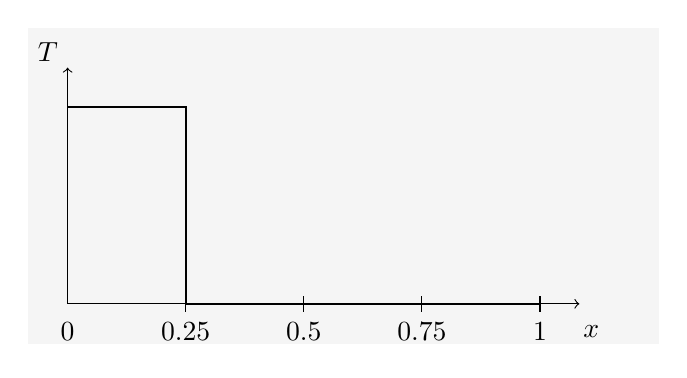
\begin{tikzpicture}
\draw[fill=gray!8,gray!8](0,0) rectangle (8,4);
%\draw[step=0.5cm,gray,very thin] (0,0) grid (8,4); %background grid

\draw[->] (0.5,0.5) -- (7,0.5) ; 
\node[] at (0.5,0.15) {$0$};

\node[] at (2,0.15) {$0.25$};
\node[] at (3.5,0.15) {$0.5$};
\node[] at (5,0.15) {$0.75$};
\node[] at (6.5,0.15) {$1$};
\draw[->] (0.5,0.5) -- (0.5,3.5) ; 
\node[] at (0.25,3.7) {$T$};


\draw[-] (2,0.4) -- (2,0.6) ; 
\draw[-] (3.5,0.4) -- (3.5,0.6) ; 
\draw[-] (5,0.4) -- (5,0.6) ; 
\draw[-] (6.5,0.4) -- (6.5,0.6) ; 


%\draw[-] (2,1) -- (1.75,0.75) ; 
%\draw[-] (2.5,1) -- (2.25,0.75) ; 
%\draw[-] (3,1) -- (2.75,0.75) ; 
%\draw[-] (3.5,1) -- (3.25,0.75) ; 
%\draw[-] (4,1) -- (3.75,0.75) ; 
%\draw[-] (4.5,1) -- (4.25,0.75) ; 

%---------------------------------

%\draw[thick,->] (7,1) -- (7,5) ; 
%\node[] at (6.6,4) {$L_y$};
%\node[] at (6.6,1) {$0$};
%\draw[-] (6.85,1) -- (7.15,1) ; 
%\draw[-] (6.85,4) -- (7.15,4) ; 
%\node[] at (7.6,4) {$p=0$};
%\node[] at (6.6,5) {$y$};

%---------------------------------

\draw[thick] (0.5,3) -- (2,3) -- (2,0.5) -- (6.5,0.5) ; 
\node[] at (7.15,0.15) {$x$};


\end{tikzpicture}



\end{center}

Set $\rho=C_p=1$.
Run the model for 250 time steps with $\delta t=0.002$.
Implement a fully implicit, explicit and Crank-Nicolson 
time discretisation. 

When using Crank-Nicolson, you should then be able to recover the green line of the 
following figure:
\begin{center}
\includegraphics[width=8cm]{images/fem_exercises/fantom3.png} \\
{\captionfont Taken from Thieulot (2011) \cite{thie11}. Note that $\tau=\gamma h/u$.}
\end{center}

Finally, implement the SUPG method and recover the red and turquoise lines.

\par\noindent\rule{\textwidth}{0.4pt}
\end{minipage}
\end{center}
%-/-/-/-/-/-/-/-/-/-/-/-/-/-/-/-/-/-/











 %---
\subsection{The advection-diffusion equation in 2D} We start from the 'bare-bones' heat transport equation (source terms are omitted): 
\begin{equation}
\rho C_p \left( \frac{\partial T}{\partial t} + {\vec \upnu}\cdot {\vec\nabla T} \right)
= {\vec \nabla} \cdot \left( k \vec\nabla T \right)
\end{equation}
In what follows we assume that the velocity vield $\vec \upnu$ is known so that temperature is the 
only unknown.
Let $N^\uptheta$ be the temperature basis functions so that the temperature inside an element is 
given by\footnote{the $\uptheta$ superscript has been chosen to denote temperature so as to avoid confusion
with the transpose operator}:
\begin{equation}
T^h({\vec r}) = \sum_{i=1}^{m_T} N^\uptheta_i ({\vec r}) T_i = \vec N^\uptheta \cdot \vec T
\end{equation}
where $\vec T$ is a vector of length $m_T$
The weak form is then 
\begin{equation}
\int_\Omega N^\uptheta_i \left[ 
\rho C_p \left( \frac{\partial T}{\partial t} + {\vec \upnu}\cdot {\vec\nabla T} \right) \right] d\Omega
= \int_\Omega  N^\uptheta_i {\vec \nabla} \cdot k \vec\nabla T  d\Omega
\end{equation}

\[
\underbrace{\int_\Omega N^\uptheta_i  \rho C_p \frac{\partial T}{\partial t} d\Omega}_{I}
+ \underbrace{\int_\Omega N^\uptheta_i  \rho C_p  {\vec \upnu}\cdot {\vec\nabla T}   d\Omega}_{II}
= \underbrace{\int_\Omega  N^\uptheta_i {\vec \nabla} \cdot k \vec\nabla T d\Omega}_{III}
\quad\quad
i=1,m_T
\]

Looking at the first term:
\begin{eqnarray}
\int_\Omega N^\uptheta_i  \rho C_p \frac{\partial T}{\partial t} d\Omega
&=&  \int_\Omega N^\uptheta_i  \rho C_p \vec N^\uptheta \cdot \dot{\vec T}  d\Omega \\
\end{eqnarray}
so that when we assemble all contributions for $i=1,m_T$ we get:
\[
I 
= \int_\Omega \vec N^\uptheta  \rho C_p \vec N^\uptheta \cdot \dot{\vec T}  d\Omega
= \left( \int_\Omega \rho C_p  \vec N^\uptheta  \vec N^\uptheta  d\Omega \right) \cdot \dot{\vec T}
= {\bm M}^T \cdot \dot{\vec T}
 \]
where ${\bm M}^T$ is the mass matrix of the system of size $(m_T \times m_T)$ with 
\[
M_{ij}^T = \int_\Omega \rho C_p N_i^\uptheta N_j^\uptheta d\Omega
\]
Turning now to the second term:
\begin{eqnarray}
\int_\Omega N^\uptheta_i  \rho C_p  {\vec \upnu}\cdot {\vec\nabla T}   d\Omega
&=& \int_\Omega N^\uptheta_i  \rho C_p (u \frac{\partial T}{\partial x} +  v \frac{\partial T}{\partial y} ) d\Omega \\
&=& \int_\Omega N^\uptheta_i  \rho C_p (u \frac{\partial \vec N^\uptheta}{\partial x} +  v \frac{\partial \vec N^\uptheta}{\partial y} ) \cdot \vec T d\Omega \\
\end{eqnarray}
so that when we assemble all contributions for $i=1,m_T$ we get:
\[
II = \left(\int_\Omega \rho C_p \vec N^\uptheta (u \frac{\partial \vec N^\uptheta}{\partial x} +  v \frac{\partial \vec N^\uptheta}{\partial y} ) d\Omega \right)  \cdot \vec T = {\bm K}_a \cdot \vec T
\]
where ${\bm K}_a$ is the advection term matrix of size $(m_T \times m_T)$ with
\[
(K_a)_{ij} = \int_\Omega \rho C_p N_i^\uptheta 
\left(u \frac{\partial N_j^\uptheta}{\partial x} +  v \frac{\partial N_j^\uptheta}{\partial y} \right) d\Omega 
\]
Now looking at the third term, we carry out an integration by part and neglect the surface term for now, so that 
\begin{eqnarray}
\int_\Omega  N^\uptheta_i {\vec \nabla} \cdot k \vec\nabla T d\Omega
&=& - \int_\Omega  k \vec \nabla N^\uptheta_i \cdot \vec\nabla T d\Omega \\
&=& - \int_\Omega  k \vec \nabla N^\uptheta_i \cdot \vec\nabla (\vec N^\uptheta \cdot \vec T) d\Omega \\
\end{eqnarray}
with 
\[
\vec \nabla \vec N^\uptheta = 
\left(
\begin{array}{cccc}
\partial_x N_1^\uptheta & 
\partial_x N_2^\uptheta & \dots &
\partial_x N_{m_T}^\uptheta \\ \\
\partial_y N_1^\uptheta & 
\partial_y N_2^\uptheta & \dots &
\partial_y N_{m_T}^\uptheta 
\end{array}
\right)
\]
so that finally:
\[
III = - \left( \int_\Omega k (\vec \nabla \vec N^\uptheta)^T \cdot \vec \nabla \vec N^\uptheta d\Omega \right) \cdot \vec T
= - {\bm K}_d \cdot \vec T
\]
where ${\bm K}_d$ is the diffusion term matrix:
\[
{\bm K}_d = \int_\Omega  k (\vec \nabla \vec N^\uptheta)^T \cdot \vec \nabla \vec N^\uptheta d\Omega 
\]
 Ultimately terms $I,II,III$ together yield:
\[
\boxed{
{\bm M}^\uptheta \cdot \dot{\vec T} + ({\bm K}_a + {\bm K}_d) \cdot \vec T = \vec 0
}
\]

%What now remains to be done is to address the time derivative on the temperature vector. 
%The most simple approach would be to use an explicit Euler one, i.e.:
%\[
%\frac{\partial \vec T}{\partial t} = \frac{\vec T^{(k)} - \vec T^{(k-1)}}{\delta t}
%\]
%where $\vec T^{(k)}$ is the temperature field at time step $k$ and $\delta t$ is the time interval 
%between two consecutive time steps.
%In this case the discretised heat transport equation is:
%\[
%\boxed{
%\left( {\bm M}^\uptheta  + ({\bm K}_a + {\bm K}_d) \delta t \right) \cdot \vec T^{(k)} =  {\bm M}^\uptheta \cdot \vec T^{(k-1)}
%}
%\]
\todo[inline]{add source term!!}

%....................................................
\subsubsection{Dealing with the time discretisation} \ref{sec:timediscr}

Essentially we have to solve a PDE of the type:
\[
\frac{\partial T}{\partial t} = {\cal F}(\vec \upnu,T,\vec\nabla T,\Delta T)
\]
with ${\cal F}=\frac{1}{\rho C_p}(-\vec\upnu\cdot\vec\nabla T + \vec\nabla\cdot k\vec\nabla T)$.

\index{general}{Forward Euler}
\index{general}{Backward Euler}
\index{general}{Crank-Nicolson}

The (explicit) forward Euler method is:
\[
\frac{T^{n+1}-T^n}{\delta t} = {\cal F}^n(T,\vec\nabla T,\Delta T)
\]
The (implicit) backward Euler method is:
\[
\frac{T^{n+1}-T^n}{\delta t} = {\cal F}^{n+1}(T,\vec\nabla T,\Delta T)
\]
and the (implicit) Crank-Nicolson algorithm is:
\[
\frac{T^{n+1}-T^n}{\delta t} = 
\frac{1}{2}
\left[
{\cal F}^{n}(T,\vec\nabla T,\Delta T)
+
{\cal F}^{n+1}(T,\vec\nabla T,\Delta T)
\right]
\]
where the superscript $n$ indicates the time step.
The Crank-Nicolson is obviously based on the trapezoidal rule, with second-order convergence in time.


In what follows, I omit the superscript on the mass matrix to simplify notations: ${\bm M}^\uptheta={\bm M}$.
In terms of Finite Elements, these become:
\begin{itemize}
\item Explicit Forward euler:
\[
\frac{1}{\delta t} ({\bm M}^{n+1} \cdot \vec T^{n+1}  -{\bm M}^n \cdot \vec T^{n} )
=
-({\bm K}_a^n+{\bm K}^n_d) \cdot \vec T^{n}
\]
or, 
\[
\boxed{
{\bm M}^{n+1} \cdot \vec T^{n+1}
= \left(  {\bm M}^n  + ({\bm K}_a^n+{\bm K}_d^n) \delta t \right)\cdot \vec T^{n} 
}
\]

\item Implicit Backward euler:
\[
\frac{1}{\delta t} ({\bm M}^{n+1} \cdot \vec T^{n+1}  -{\bm M}^n \cdot \vec T^{n} )
= -({\bm K}_a^{n+1}+{\bm K}_d^{n+1}) \cdot \vec T^{n+1}
\]
or, 
\begin{equation}
\boxed{
\left( {\bm M}^{n+1} +({\bm K}_a^{n+1}+{\bm K}_d^{n+1})\delta t \right) \cdot \vec T^{n+1}
=
{\bm M}^n \cdot \vec T^{n} 
}
\label{eq:hte_ibe}
\end{equation}

\item Crank-Nicolson

\[
\frac{1}{\delta t} \left({\bm M}^{n+1} \cdot \vec T^{n+1}  -{\bm M}^n \cdot \vec T^{n} \right)
= 
\frac{1}{2}
\left[
-({\bm K}_a^{n+1}+{\bm K}_d^{n+1}) \cdot \vec T^{n+1}
-({\bm K}_a^{n}+{\bm K}_d^{n}) \cdot \vec T^{n}
\right]
\]
or,
\[
\boxed{
\left( {\bm M}^{n+1} +({\bm K}_a^{n+1}+{\bm K}_d^{n+1})\frac{\delta t}{2} \right) \cdot \vec T^{n+1}
= \left(  {\bm M}^n  + ({\bm K}_a^n+{\bm K}_d^n) \frac{\delta t}{2} \right)\cdot \vec T^{n} 
}
\]

Note that in benchmarks where the domain/grid does not deform, the coefficients do not change in space
and the velocity field is constant in time, or in practice out of convenience, the ${\bm K}$  and ${\bm M}$ 
matrices do not change and the r.h.s. can be constructed with the same matrices as the FE matrix.

\end{itemize}




\index{general}{BDF-2}
\paragraph{The Backward differentiation formula} (see for instance \cite{hawa91} or Wikipedia\footnote{\url{https://en.wikipedia.org/wiki/Backward_differentiation_formula}}. The second-order BDF (or BDF-2) as shown in \cite{krhb12} is as follows: it is a finite-difference 
quadratic interpolation approximation of the $\partial T/\partial t$ term which involves
$t^n$, $t^{n-1}$ and $t^{n-2}$:
\begin{equation}
\frac{\partial T}{\partial t}(t^n) =
\frac{1}{\tau_n} \left( \frac{2\tau_n + \tau_{n-1}}{\tau_n+\tau_{n-1} } T(t^n)  
- \frac{\tau_n +\tau_{n-1}}{\tau_{n-1}} T(t^{n-1})
+ \frac{\tau_n^2}{\tau_{n-1}(\tau_n+\tau_{n-1})} T(t^{n-2})
\right)
\end{equation}
where $\tau_n=t^n-t^{n-1}$.
Starting again from 
${\bm M}^\uptheta \cdot \dot{\vec T} + ({\bm K}_a + {\bm K}_d) \cdot \vec T = \vec 0$,
we write 
\[
{\bm M}^\uptheta \cdot 
\frac{1}{\tau_n} \left( \frac{2\tau_n + \tau_{n-1}}{\tau_n+\tau_{n-1} } \vec T^n  
- \frac{\tau_n +\tau_{n-1}}{\tau_{n-1}} \vec T^{n-1}
+ \frac{\tau_n^2}{\tau_{n-1}(\tau_n+\tau_{n-1})} \vec T^{n-2} \right)
+ ({\bm K}_a + {\bm K}_d) \cdot \vec T^n = \vec 0
\]
and finally:
\[
\left[
\frac{2\tau_n + \tau_{n-1}}{\tau_n+\tau_{n-1} }
{\bm M}^\uptheta
+ \tau_n({\bm K}_a + {\bm K}_d)
\right]
 \cdot \vec T^n =
 \frac{\tau_n +\tau_{n-1}}{\tau_{n-1}} {\bm M}^\uptheta \cdot \vec T^{n-1}
- \frac{\tau_n^2}{\tau_{n-1}(\tau_n+\tau_{n-1})} {\bm M}^\uptheta \cdot \vec T^{n-2}
\]
Note that if all timesteps are equal, i.e. $\tau_n=\tau_{n-1}=\delta t$, this equation becomes:
\[
\left[
\frac{3}{2}
{\bm M}^\uptheta
+ \delta t({\bm K}_a + {\bm K}_d)
\right]
 \cdot \vec T^n =
{\bm M}^\uptheta \cdot \left(2 \vec T^{n-1} - \frac{1}{2} \vec T^{n-2} \right)
\]
or, 
\[
\left[
{\bm M}^\uptheta
+ \frac{2}{3}\delta t({\bm K}_a + {\bm K}_d)
\right]
 \cdot \vec T^n =
{\bm M}^\uptheta \cdot \left( \frac{4}{3} \vec T^{n-1} - \frac{1}{3} \vec T^{n-2} \right)
\]

As mentioned before the 
backward differenciation formula (BDF) is a family of implicit methods
for the integration of ODEs. Each BDF-$s$ method achieves order $s$.
The BDF-1 is simply the backward Euler method as seen above:
\[
T^{n+1}-T^n=\delta t {\cal F}^{n+1}
\]
The BDF-2 is given by 
\[
T^{n+2} - \frac{4}{3}T^{n+1} +\frac{1}{3} T^n = \frac{2}{3} \delta t {\cal F}^{n+2}
\]
The BDF-3 is given by 
\[
T^{n+3} - \frac{18}{11}T^{n+2} +\frac{9}{11} T^{n+1} -\frac{2}{11}T^n = \frac{6}{11} \delta t {\cal F}^{n+3}
\]
The BDF-4 is given by 
\[
T^{n+4}-\frac{48}{25}T^{n+1}+\frac{36}{25}T^{n+1}-\frac{16}{25}T^{n+1}+\frac{3}{25}T^n = \frac{12}{25}\delta t {\cal F}^{n+4}
\]


%....................................................
\subsubsection{On steady states}

It is said that a system is in a steady state if the (state) variables which define the behavior of the system 
are unchanging in time. In continuous time, this means that the partial derivative with respect to time is zero and remains so:
\[
\frac{\partial}{\partial t} =0 \qquad \forall t
\]
This is irrelevant for the Stokes equations which do not contain an explicit time dependence but the heat 
transport equation can reach a steady state. 
Note that if one is only interested in the steady state solution (and not how the system gets there in time)
then the heat transport equation should be solved with $\partial T/\partial t$ set to zero. 

%....................................................
\subsubsection{Anisotropic heat conduction}\label{sec:anisotropic}

\index{general}{Isotropic}\index{general}{Orthotropic}

It is most often assumed that the heat conductivity is isotropic so that one speaks of heat conductivity as a 
scalar $k$.  However many materials are orthotropic and in that case the heat conductivity is a tensor ${\bm k}$
which (in 2D) writes \cite[p121]{reddybook2}:
\[
{\bm k}
=
\left(
\begin{array}{cc}
k_{xx} & k_{xy} \\
k_{yx} & k_{yy}
\end{array}
\right)
=
\left(
\begin{array}{cc}
\cos\theta & \sin\theta \\
-\sin\theta & \cos\theta
\end{array}
\right)
\cdot
\left(
\begin{array}{cc}
k_1 & 0 \\ 0 & k_2
\end{array}
\right)
\cdot
\left(
\begin{array}{cc}
\cos\theta & -\sin\theta \\
\sin\theta & \cos\theta
\end{array}
\right)
\]
where $k_1$ and $k_2$ are the conductivities in the principal axes system and $\theta$ is 
the local orientation.
In that case the diffusion term in the heat trasport equation becomes $\vec{\nabla}\cdot({\bm k}\cdot \vec{\nabla}T)$.


\mscthesis: \cite[p121]{reddybook2}, \cite[p143]{reddybook2} \index{general}{MSc Thesis}


%....................................................
\subsubsection{About the assembly}

Let us consider for simplicity the following grid composed of 9 nodes and 4 $Q_1$ elements. 
Each node carries a single degree of freedom. 

\begin{center}
\includegraphics[width=12cm]{images/assembly/assembly.png} 
\end{center}

There are four elements:
\begin{itemize}
\item element 1 is composed of nodes $(1,2,5,4)={\vec T}^{el1}$
\item element 2 is composed of nodes $(2,3,6,5)={\vec T}^{el2}$
\item element 3 is composed of nodes $(4,5,8,7)={\vec T}^{el3}$
\item element 4 is composed of nodes $(5,6,9,8)={\vec T}^{el4}$
\end{itemize}
For each element one has computed an elemental matrix ${\bm A}^{el}$ and a right hand side ${\vec b}^{el}$. 
\[
{\bm A}^{el1} \cdot {\bm T}^{el1} = {\bm b}^{el1}
\]
\[
{\bm A}^{el2} \cdot {\bm T}^{el2} = {\bm b}^{el2}
\]
\[
{\bm A}^{el3} \cdot {\bm T}^{el3} = {\bm b}^{el3}
\]
\[
{\bm A}^{el4} \cdot {\bm T}^{el4} = {\bm b}^{el4}
\]
As seen in the 1D case, these four linear systems must be assembled in a single large matrix of size 
$9\times 9$ as shown in the figure above.

 %-----------------------

\newpage 
%%%%%%%%%%%%%%%%%%%%%%%%%%%%%%%%%%%%%%%%%%%%%%%%%%%%%%%%%%%%%%%%%%%%%%%%%%%%%%%%%%%%%%%%%
\section{Solving the flow equations with the FEM} \label{solvingFEM} %%%%%%%%%%%%%%%%%%%%
%6.3 of donea and huerta

In the case of an incompressible flow, we have seen that the continuity (mass conservation)
equation takes the simple form ${\vec \nabla}\cdot{\vec \upnu}=0$. In other words flow takes place 
under the constraint that the divergence of its velocity field is exactly zero eveywhere 
(solenoidal constraint), i.e. it is divergence free. 
\index{general}{Divergence-free Flow} 
\index{general}{Solenoidal Field}

We see that the pressure in the momentum equation is then a degree of freedom which is needed 
to satisfy the incompressibilty constraint (and it is not related to any constitutive equation)
\cite{dohu03}. In other words the pressure is acting as a Lagrange multiplier of the incompressibility
constraint. 

Various approaches have been proposed in the literature to deal with the 
incompressibility constraint but we will only focus on the penalty method 
(section \ref{sec:penalty}) and the so-called mixed finite element method
\ref{sec:mixed}.
 %-----------------------------------------------------------------
\subsection{Strong and weak forms} \begin{flushright} {\tiny {\color{gray} strongweak.tex}} \end{flushright}

\index{general}{strong form} 

The strong form consists of the governing equation and the boundary conditions, i.e. 
the mass, momentum and energy conservation equations supplemented with Dirichlet and/or Neumann
boundary conditions on (parts of) the boundary.


\index{general}{weak form}
To develop the finite element formulation, the partial differential equations 
must be restated in an integral form called the weak form. In essence the PDEs are 
first multiplied by an arbitrary function and integrated over the domain.

 

 %----------------------------------
\subsection{Which velocity-pressure pair for Stokes?} 

The success of a mixed finite element formulation crucially depends on a proper choice of the local interpolations of the velocity and the pressure. 

%........................................................................................
\subsubsection{The compatibility condition (or LBB condition, or inf-sup condition)} \label{ss:LBBcond}
\index{general}{LBB} \index{general}{Optimal Rate}

WARNING: I am not comfortable writing about this topic. What follows is a rough attempt at making sense of it.


The Lady{\v z}henskaya-Babu{\v s}ka-Brezzi (LBB) condition is a sufficient 
condition for a saddle point problem to have a unique solution.
For saddle point problems coming from the Stokes equations, 
many discretizations are unstable, giving rise to artifacts such as spurious oscillations. 
The LBB condition gives criteria for when a discretization of a saddle point problem is stable. 
It also assures convergence at the optimal rate. 

Bochev \& Gunzburger \cite{bogu09} state: "
The terminology “LBB” originates from the facts that this condition was first explicitly discussed
in the finite element setting for saddle point problems by Brezzi \cite{brez74} and that it is a special case of
the general weak-coercivity condition first discussed for finite element methods by Babu{\v s}ka
\cite{babu71} and that, in the continuous setting of the Stokes equation, this condition was first proved to
hold by Ladyzhenskaya; see \cite{lady69}."

Unfortunately, to quote Donea \& Huerta \cite{dohu03}: 
"In the finite element context, it is by no means easy to prove whether or not a given
velocity-pressure pair satisfies the LBB compatibility condition."
Elman et al state: "[...] Choosing spaces for which the discrete inf-sup condition holds
and is a delicate matter, and seemingly natural choices of velocity and pressure approximation
do not work. [...] In general, care must be taken to make the velocity space 
rich enough compared to the pressure space."

The LBB condition, or inf-sup condition can be proven in different ways, and standard techniques have been designed
as listed in Boffi et al (2008) \cite{bobf08}.

%p129
Elman et al \cite{elsw} state that "The inf-sup condition is a sufficient condition for the pressure to be unique up
to  constant in the case of an enclosed flow." This can also be proven for other boundary conditions.
This approach, based on the macro-element technique \cite{sten90} is explored in Appendix \ref{app:Gel}.


It can be shown that, provided the kernel (null space) of matrix $\G$ is zero,
the Stokes matrix is non-singular, that is $\vec{\cal V}$ and $\vec{\cal P}$ 
are uniquely defined, and the Schur complement matrix $\SSS$ is positive definite. 
Simply put, taking $\vec{\cal V}=\vec{0}$ in the discretised Stokes system 
without body forces yields $\G \cdot \vec{\cal P}=\vec{0}$ and implies
that any pressure solution is only unique up to the null space of the matrix $\G$.

We know that the Schur complement matrix $\SSS$ is positive definite if and only if all of its eigenvalues are positive.
One could then (numerically) compute the eigenvalues of $\SSS$ and check that these are indeed strictly positive
to show that $\SSS$ is pos def. 

%Since $\SSS$ is trivially symmetric (because $\K$ is symmetric), then 

Another way is to see that $\SSS$ is positive definite only if $\text{ker}(\G)=\{0\}$.
Again to quote Donea \& Huerta \cite{dohu03}: "If this is the case, the partitioned Stokes matrix  
is non-singular and delivers uniquely defined velocity and pressure fields. If this is not the case, a
stable and convergent velocity field might be obtained, but the pressure field is likely
to present spurious and oscillatory results." 
Note that in the case of the $Q_1 \times P_0$ element it has been shown that the multiple families of 
checkboard pressure modes actually lie in the kernel of $\G$. \cite{XXXXsani}

One could then also numerically compute the Ker of G?

\vspace{.4cm}

LBB means velocity and pressure spaces yield uniquely defined vel and p solutions. 
is proving ker(G)=0 enough? is proving S (S)PD enough ?

Check \cite{chba93}


%........................................................................................
\subsubsection{Families}
\index{general}{Taylor-Hood}

The family of \underline{Taylor-Hood} finite element spaces on triangular/tetrahedral 
grids is given by $P_k \times P_{k-1}$ with $k\geq 2$, 
and on quadrilateral/hexahedral grids by $Q_k \times Q_{k-1}$ with $k\geq 2$.
This means that the pressure is then approximated by continuous functions. 

These finite elements are very popular, in particular the pairs for $k=2$, i.e.
$Q_2\times Q_1$ and $P_2\times P_1$.
The reason why $k\geq 2$ comes from the fact that the 
$Q_1 \times Q_0$ (i.e. $Q_1 \times P_0$) and $P_2\times P_1$
are not stable elements (they are not inf-sup stable). 

\begin{remark}
Note that a similar element to $Q_2 \times Q_1$ has been proposed
and used succesfully used \cite{taho73,hota74}: it is denoted by $Q_2^{(8)} \times Q_1$ 
since the center node ('$x^2y^2$') and its associated degrees of freedom have been removed. It 
has also been proved to be LBB stable. 
\end{remark}


The \underline{Raviart-Thomas} family\todo{find literature} on triangles and quadrilaterals.

%........................................................................................
\subsubsection{The bi/tri-linear velocity - constant pressure element ($Q_1\times P_0$)}

\begin{minipage}[t]{0.5\textwidth}
\begin{flushright} {\tiny {\color{gray} (tikz\_q1p0.tex)}} \end{flushright}
%~~~~~~~~~~~~~~~~~~~~~~~~~~~~~~~~~~~~~~~~~~~~~~~~~~~~~~~~~~~~~~~~~~~~~~~~~~~~~~~~~~~~~~~~~~~~~~~~~~

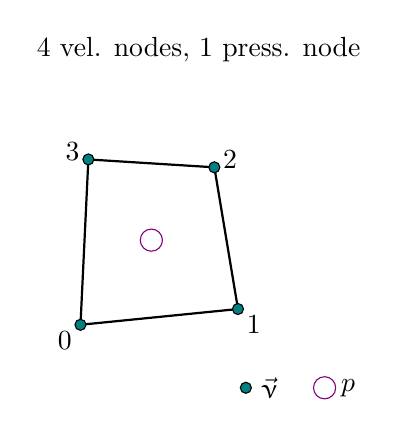
\begin{tikzpicture}
%\draw[fill=gray!23,gray!23](0,0) rectangle (5,5);
%\draw[step=0.5cm,gray,very thin] (0,0) grid (4,4); %background grid
\draw[thick] (1,1) -- (3,1.2) -- (2.7,3) -- (1.1,3.1) -- cycle;  
\node[] at (0.8,0.8) {0};
\node[] at (3.2,1) {1};
\node[] at (2.9,3.1) {2};
\node[] at (0.9,3.2) {3};
\draw[violet] (1.9,2.075) circle (4pt);
\draw[black,fill=teal] (1,1)   circle (2pt);
\draw[black,fill=teal] (3,1.2)  circle (2pt);
\draw[black,fill=teal] (2.7,3)  circle (2pt);
\draw[black,fill=teal] (1.1,3.1) circle (2pt);
\draw[black,fill=teal] (3.1,0.2) circle (2pt); 
\node[] at (3.4,0.2) {$\vec\upnu$};
\draw[violet] (4.1,0.2) circle (4pt); 
\node[] at (4.4,0.2) {$p$};
\node[] at (2.5,4.5) {4 vel. nodes, 1 press. node};
\end{tikzpicture}

\end{minipage}
\begin{minipage}[t]{0.5\textwidth}

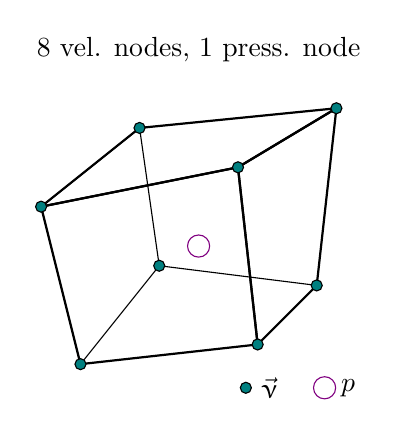
\begin{tikzpicture}
%\draw[fill=gray!23,gray!23](0,0) rectangle (5,5);
%\draw[step=0.25cm,gray,very thin] (0,0) grid (5,4); %background grid
\draw[thick] (1,0.5) -- (3.25,0.75) -- (3,3) -- (0.5,2.5) -- cycle; %1-2-6-5
\draw[thick] (3.25,0.75) -- (4,1.5) -- (4.25,3.75) -- (3,3) -- cycle; %2-3-7-6
\draw[thick] (0.5,2.5) -- (3,3) -- (4.25,3.75) -- (1.75,3.5) -- cycle; %5-6-7-4
\draw[thin]   (1,0.5) -- (2,1.75) -- (1.75,3.5) -- (0.5,2.5)   --cycle; % 1-0-4-5 
\draw[thin] (2,1.75) -- (4,1.5); 
%\node[] at (0.8,0.8) {0};
%\node[] at (3.2,1) {1};
%\node[] at (2.9,3.1) {2};
%\node[] at (0.9,3.2) {3};
\draw[violet] (2.5,2.) circle (4pt);
\draw[black,fill=teal] (1,0.5)   circle (2pt);
\draw[black,fill=teal] (3.25,0.75)   circle (2pt);
\draw[black,fill=teal] (3,3)   circle (2pt);
\draw[black,fill=teal] (0.5,2.5)   circle (2pt);
\draw[black,fill=teal] (1.75,3.5)  circle (2pt);
\draw[black,fill=teal] (4.25,3.75)  circle (2pt);
\draw[black,fill=teal] (4,1.5) circle (2pt);
\draw[black,fill=teal] (2,1.75) circle (2pt);
\draw[black,fill=teal] (3.1,0.2) circle (2pt); 
\node[] at (3.4,0.2) {$\vec\upnu$};
\draw[violet] (4.1,0.2) circle (4pt); 
\node[] at (4.4,0.2) {$p$};
\node[] at (2.5,4.5) {8 vel. nodes, 1 press. node};
\end{tikzpicture}

\end{minipage}

discussed in example 3.71 of \cite{john16}

However simple it may look, the \index{general}{$Q_1 \times P_0$} element is 
one of the hardest elements to analyze and many questions are still open about its properties. 
The element does not satisfy the inf-sup condition \cite{hugh}p211. 
In \cite{grsa} it is qualified as follows: slightly unstable but highly usable. 

The $Q_1 \times P_0$ mixed approximation is the lowest order conforming approximation 
method defined on a rectangular grid. It also happens to be the most famous example 
of an unstable mixed approximation method.
\cite[p235]{elsw}.

This element is discussed in \cite{fort81}, \cite{fofo85} and in \cite{pisa85} 
in the context of multigrid use.

This element is plagued by so-called pressure checkerboard modes which
have been thoroughly analysed \cite{grsi94}, \cite{chpc95}, \cite{sagl81a,sagl81b}.
These can be filtered out \cite{chpc95}. Smoothing techniques are also discussed in \cite{legs79}.

\Literature \cite{fobo90}\cite{grle85}\cite{leru86}



%----------------------------------------------------------------------
\subsubsection{The bi/tri-quadratic velocity - discontinuous linear pressure element ($Q_2 \times P_{-1}$)}

This element is crowned "probably the most accurate 2D element" in Gresho \& Sani's book \cite{grsa}.

It is characterised by piecewise Biquadratic velocities, 
and piecewise linear discontinuous polynomial pressure. 
The element satisfies the inf-sup condition, see page 211 of Hughes \cite{hugh}, or p138 of Elman et al
\cite{elsw}.
It is used in van de Vosse et al (1989) \cite{vavs89} for steady laminar flowin a curved tube. 
See Boffi \& Gastaldi (2002) \cite{boga02} 
for the two possible choices for the definition of the pressure space..
This element is mentioned in Kaus (2010) \cite{kaus10} and Pelletier et al (1989) \cite{pefc89} 
and it is  used in Frehner (2014) \cite{freh14} to study 3D fold growth rates 
(see online supplementary material) and in Schmalholtz (2008) \cite{schm08}.

Note that the serendipity version of this pair, i.e. $Q_2^{(20)}\times P_{-1}$ is also LBB stable
as shown in p180 of Reddy \cite{reddybook2}.

This element is implemented in Stone 76. 

\begin{center}
\includegraphics[width=6cm]{images/q2pm1/q2pm1}
\end{center}


%----------------------------------------------------------------------
\subsubsection{The bi/tri-quadratic velocity - bi/tri-linear pressure element ($Q_2 \times Q_1$)}
\label{ss:pairq2q1}

\begin{minipage}[t]{0.5\textwidth}
\begin{flushright} {\tiny {\color{gray} (tikz\_q2q1.tex)}} \end{flushright}
%~~~~~~~~~~~~~~~~~~~~~~~~~~~~~~~~~~~~~~~~~~~~~~~~~~~~~~~~~~~~~~~~~~~~~~~~~~~~~~~~~~~~~~~~~~~~~~~~~~

%\begin{center}
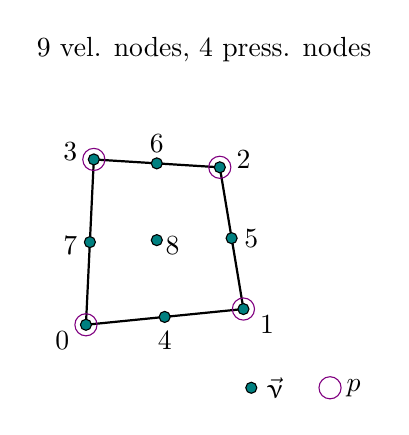
\begin{tikzpicture}
%\draw[fill=gray!23,gray!23](0,0) rectangle (5,5);
%\draw[step=0.5cm,gray,very thin] (0,0) grid (4,4); %background grid
\draw[thick] (1,1) -- (3,1.2) -- (2.7,3) -- (1.1,3.1) -- cycle;  
\node[] at (0.7,0.8) {0};
\node[] at (3.3,1) {1};
\node[] at (3,3.1) {2};
\node[] at (0.8,3.2) {3};
\draw[black,fill=teal] (1,1)     circle (2pt); \draw[violet] (1,1) circle (4pt);
\draw[black,fill=teal] (3,1.2)   circle (2pt); \draw[violet] (3,1.2) circle (4pt);
\draw[black,fill=teal] (2.7,3)   circle (2pt); \draw[violet] (2.7,3) circle (4pt);
\draw[black,fill=teal] (1.1,3.1) circle (2pt); \draw[violet] (1.1,3.1) circle (4pt);
\draw[black,fill=teal] (2,1.1) circle (2pt) ; \node[] at (2,0.8) {4};
\draw[black,fill=teal] (2.85,2.1) circle (2pt) ; \node[] at (3.1,2.1) {5};
\draw[black,fill=teal] (1.9,3.05) circle (2pt) ; \node[] at (1.9,3.3) {6};
\draw[black,fill=teal] (1.05,2.05) circle (2pt) ; \node[] at (0.8,2) {7};
\draw[black,fill=teal] (1.9,2.075) circle (2pt) ; \node[] at (2.1,2) {8};
\draw[black,fill=teal] (3.1,0.2) circle (2pt); 
\node[] at (3.4,0.2) {$\vec\upnu$};
\draw[violet] (4.1,0.2) circle (4pt); 
\node[] at (4.4,0.2) {$p$};
\node[] at (2.5,4.5) {9 vel. nodes, 4 press. nodes};
\end{tikzpicture}
%\end{center}

\end{minipage}
\begin{minipage}[t]{0.5\textwidth}



%\begin{center}
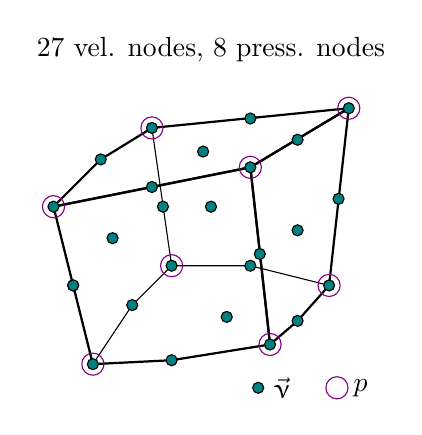
\begin{tikzpicture}
%\draw[fill=gray!23,gray!23](0,0) rectangle (5,5);
%\draw[step=0.5cm,gray,very thin] (0,0) grid (5,4); %background grid
\draw[thick] (1,0.5) -- (2,0.55) --(3.25,0.75) -- (3,3) -- (0.5,2.5) -- cycle; %1-9-2-6-5
\draw[thick] (3.25,0.75) -- (3.6,1.05) -- (4,1.5) -- (4.25,3.75) -- (3,3) -- cycle; %2-10-3-7-6
\draw[thick] (0.5,2.5) -- (3,3) -- (4.25,3.75) -- (1.75,3.5) -- (1.1,3.1) -- cycle; %5-6-7-4-13
\draw[thin]   (1,0.5) -- (1.5,1.25) -- (2,1.75) -- (1.75,3.5) -- (1.1,3.1) -- (0.5,2.5) --cycle; % 1-8-0-4-5-13 
\draw[thin] (2,1.75) -- (3,1.75) -- (4,1.5); %0-11-3
%pressure nodes
\draw[violet] (2,1.75) circle (4pt); % 0 
\draw[violet] (1,0.5) circle (4pt); % 1 
\draw[violet] (3.25,0.75) circle (4pt); % 2 
\draw[violet] (4,1.5) circle (4pt); % 3 
\draw[violet] (1.75,3.5) circle (4pt); % 4 
\draw[violet] (0.5,2.5) circle (4pt); % 5 
\draw[violet] (3,3) circle (4pt); % 6 
\draw[violet] (4.25,3.75) circle (4pt); % 7 
%velocity nodes
\draw[black,fill=teal] (1,0.5)   circle (2pt);
\draw[black,fill=teal] (3.25,0.75)   circle (2pt);
\draw[black,fill=teal] (3,3)   circle (2pt);
\draw[black,fill=teal] (0.5,2.5)   circle (2pt);
\draw[black,fill=teal] (1.75,3.5)  circle (2pt);
\draw[black,fill=teal] (4.25,3.75)  circle (2pt);
\draw[black,fill=teal] (4,1.5) circle (2pt);
\draw[black,fill=teal] (2,1.75) circle (2pt);
\draw[black,fill=teal] (1.5,1.25) circle (2pt); % 8 
\draw[black,fill=teal] (2,0.55) circle (2pt); % 9 
\draw[black,fill=teal] (3.6,1.05) circle (2pt); % 10
\draw[black,fill=teal] (3,1.75) circle (2pt); % 11
\draw[black,fill=teal] (0.75,1.5) circle (2pt); % 12
\draw[black,fill=teal] (1.1,3.1) circle (2pt); % 13
\draw[black,fill=teal] (0.75,1.5) circle (2pt); % 18
\draw[black,fill=teal] (2.7,1.1) circle (2pt); % 21
\draw[black,fill=teal] (3.6,3.35) circle (2pt); % 21
\draw[black,fill=teal] (3.,3.62) circle (2pt); % 21
\draw[black,fill=teal] (4.12,2.6) circle (2pt); % 21
\draw[black,fill=teal] (1.89,2.5) circle (2pt); % 21
\draw[black,fill=teal] (1.75,2.75) circle (2pt); % 21
\draw[black,fill=teal] (3.12,1.9) circle (2pt); % 21
\draw[black,fill=teal] (3.6,2.2) circle (2pt); % 21
\draw[black,fill=teal] (1.25,2.1) circle (2pt); % 21
\draw[black,fill=teal] (2.4,3.2) circle (2pt); % 21
\draw[black,fill=teal] (2.5,2.5) circle (2pt); % 21

% legend
\draw[black,fill=teal] (3.1,0.2) circle (2pt); \node[] at (3.4,0.2) {$\vec\upnu$};
\draw[violet] (4.1,0.2) circle (4pt); 
\node[] at (4.4,0.2) {$p$};
\node[] at (2.5,4.5) {27 vel. nodes, 8 press. nodes};
\end{tikzpicture}
%\end{center}


\end{minipage}


In \cite{grsa} Gresho \& Sani write that in their opinion $div(\vec v)=0$ is not strong enough.

This element, implemented in penalised form, is discussed in \cite{been79} and the follow-up paper \cite{been80}. CHECK

Biquadratic velocities, bilinear pressure. See Hood and Taylor. The element satisfies the inf-sup condition \cite{hugh}p215. 

\begin{center}
\includegraphics[width=6cm]{images/q2q1/q2numering}
\end{center}

%----------------------------------------------------------------------
\subsubsection{The stabilised bi/tri-linear velocity -  constant pressure element ($Q_1\times P_0$-stab)}

\Literature: \cite{sike90,vibo92,kesi92,qizh07,lisi12,chco01,chri02}

%----------------------------------------------------------------------
\subsubsection{The stabilised bi/tri-linear velocity -  bi/tri-linear pressure element ($Q_1\times Q_1$-stab)}

\begin{minipage}[t]{0.5\textwidth}

\begin{center}
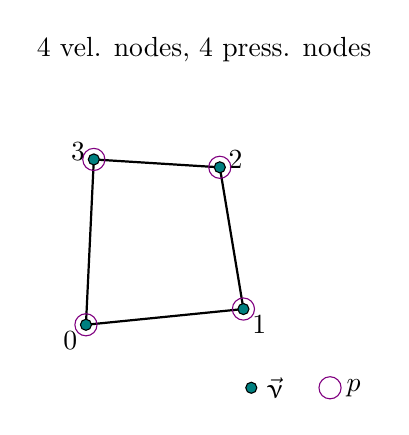
\begin{tikzpicture}
%\draw[fill=gray!23,gray!23](0,0) rectangle (5,5);
%\draw[step=0.5cm,gray,very thin] (0,0) grid (4,4); %background grid
\draw[thick] (1,1) -- (3,1.2) -- (2.7,3) -- (1.1,3.1) -- cycle;  
\node[] at (0.8,0.8) {0};
\node[] at (3.2,1)   {1};
\node[] at (2.9,3.1) {2};
\node[] at (0.9,3.2) {3};
\draw[black,fill=teal] (1,1)     circle (2pt); \draw[violet] (1,1) circle (4pt);
\draw[black,fill=teal] (3,1.2)   circle (2pt); \draw[violet] (3,1.2) circle (4pt);
\draw[black,fill=teal] (2.7,3)   circle (2pt); \draw[violet] (2.7,3) circle (4pt);
\draw[black,fill=teal] (1.1,3.1) circle (2pt); \draw[violet] (1.1,3.1) circle (4pt);
\draw[black,fill=teal] (3.1,0.2) circle (2pt); 
\node[] at (3.4,0.2) {$\vec\upnu$};
\draw[violet] (4.1,0.2) circle (4pt); 
\node[] at (4.4,0.2) {$p$};
\node[] at (2.5,4.5) {4 vel. nodes, 4 press. nodes};
\end{tikzpicture}\\
\end{center}

\end{minipage}
\begin{minipage}[t]{0.5\textwidth}

\begin{center}
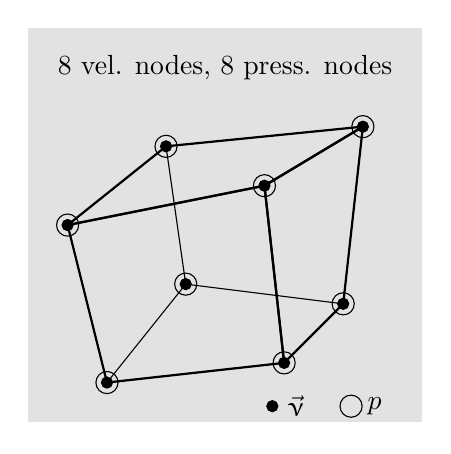
\begin{tikzpicture}
\draw[fill=gray!23,gray!23](0,0) rectangle (5,5);
%\draw[step=0.25cm,gray,very thin] (0,0) grid (5,4); %background grid
\draw[thick] (1,0.5) -- (3.25,0.75) -- (3,3) -- (0.5,2.5) -- cycle; %1-2-6-5
\draw[thick] (3.25,0.75) -- (4,1.5) -- (4.25,3.75) -- (3,3) -- cycle; %2-3-7-6
\draw[thick] (0.5,2.5) -- (3,3) -- (4.25,3.75) -- (1.75,3.5) -- cycle; %5-6-7-4
\draw[thin]   (1,0.5) -- (2,1.75) -- (1.75,3.5) -- (0.5,2.5)   --cycle; % 1-0-4-5 
\draw[thin] (2,1.75) -- (4,1.5); 
%\node[] at (0.8,0.8) {0};
%\node[] at (3.2,1) {1};
%\node[] at (2.9,3.1) {2};
%\node[] at (0.9,3.2) {3};
\draw (1,0.5) circle (4pt);
\draw (3.25,0.75) circle (4pt);
\draw (4,1.5) circle (4pt);
\draw (2,1.75) circle (4pt);
\draw (0.5,2.5) circle (4pt);
\draw (3,3) circle (4pt);
\draw (4.25,3.75) circle (4pt);
\draw (1.75,3.5) circle (4pt);
\draw[black,fill=black] (1,0.5)   circle (2pt);
\draw[black,fill=black] (3.25,0.75)   circle (2pt);
\draw[black,fill=black] (3,3)   circle (2pt);
\draw[black,fill=black] (0.5,2.5)   circle (2pt);
\draw[black,fill=black] (1.75,3.5)  circle (2pt);
\draw[black,fill=black] (4.25,3.75)  circle (2pt);
\draw[black,fill=black] (4,1.5) circle (2pt);
\draw[black,fill=black] (2,1.75) circle (2pt);
\draw[black,fill=black] (3.1,0.2) circle (2pt); \node[] at (3.4,0.2) {$\vec\upnu$};
\draw (4.1,0.2) circle (4pt); \node[] at (4.4,0.2) {$p$};
\node[] at (2.5,4.5) {8 vel. nodes, 8 press. nodes};
\end{tikzpicture}\\
\end{center}

\end{minipage}

See \cite{nosi01} for a fourier analysis of the normal and stablised (a la \cite{hufb86}) $Q_1-Q_1$ element.
This element is used in \cite{bugs09,busa13} in conjunction with AMR. 
Stabilisation is worked out out in \cite{dobo04,bodg06,bodo06}.

$Q_1\times P_0$-stab. Pro: stabilisation can be switched off; Con: stabilisation for deformed elements? 
problem near boundaries: incomplete stencil? choice of parameter $\beta$.

$Q_1\times Q_1$-stab. Pro: easier to implement than $Q_1\times P_0$-stab, stabilisation local to element, easier when elements are not rectangular, no free parameter; Con: stabilisation cannot be switched off.

\Literature: \cite{shry78,temr92,tezd92,grcc95,idsn95,knto00,fros07,lihc09}. See Braack \& Lube \cite{brlu09}
for a review of local projection stabilisation for incompressible flow problems. 

This unstable pair is also used in ice sheet modelling \cite{heah18,zhjg11,zwgg07}
A $P_1\times P_1$ version of it is used in \cite{kahp20}.


%----------------------------------------------------------------------
\subsubsection{The MINI triangular element ($P_1^+\times P_1$) in 2D}
\label{pair:mini}

The \index{general}{MINI element} MINI element was first introduced in Arnold et al, 1984 \cite{arbf84}.
It is also discussed in section 3.6.1 of \cite{john16}.
It is schematically represented hereunder:

\begin{center}
\includegraphics[width=8cm]{images/mini/minielement}\\
{\captionfont Figure taken from Donea and Huerta \cite{dohu03}}
\end{center}

\begin{remark}
Note that \cite{frol03} propose an equal-order-linear-continuous velocity-pressure variables which is enriched 
with velocity {\it and} pressure bubble functions to model the Stokes problem. They show by static condensation that
these bubble functions give rise to a stabilized method involving least-squares forms of the momentum and of the
continuity equations. In some cases their approach recovers the MINI element. Also check \cite{gamt08}.
\end{remark}

\begin{remark}
According to Braess\cite{braess}, since the support of the bubble is restricted to the element, 
the associated variable (dofs living on the bubble) can be eliminated from the resulting 
system of linear equations by static condensation. \index{general}{Static Condensation}
Also, the MINI element is cheaper than the Taylor-Hood element but it is commonly accepted
that it yields a poorer approximation of the pressure.
\end{remark}

The 3D MINI element is not very common but it is used for instance in \cite{pico98}.
It is also said to be LBB stable in \cite[p180]{reddybook2}.

\begin{center}
\includegraphics[width=10cm]{images/mini/mini3D}\\
{\captionfont Velocity and pressure nodes for the 3D MINI element, taken from \cite{pico98}}
\end{center}

Note that this element is used in \cite{brwr00} in the context of Arbitrary Lagrangian Eulerian 
finite element analysis of free surface flows.
Also used in Zlotnik et al (2007) \cite{zldf07} for suduction with X-FEM technique.







%----------------------------------------------------------------------
\subsubsection{The quadratic velocity - linear pressure triangle ($P_2\times P_1$)}

From \cite{segal}: \say{Taylor-Hood elements \cite{taho73} 
are characterized by the fact that the pressure is continuous in the region $\Omega$. 
A typical example is the quadratic triangle (P2P1 element).
In this element the velocity is approximated by a quadratic polynomial and the pressure by a
linear polynomial. One can easily verify that both approximations are continuous over 
the element boundaries.}
It can be shown, Segal (1979), that this element is admissible if at least 3 elements 
are used. The quadrilateral counterpart of this triangle is the $Q_2\times Q_1$ element.
Reddy and Gartling \cite[p179]{reddybook2} also report this element to be LBB stable.

\Literature: \cite{scan85,lejx14,cump20}


%----------------------------------------------------------------------
\subsubsection{The Crouzeix-Raviart triangle ($P_2^+\times P_{-1}$)}
\label{sec:crouzeix-raviart}

Since the $P_2\times P_{-1}$ pair is not LBB stable \cite[p179]{reddybook2}, 
it is enhanced by a cubic bubble and is therefore called $P_2^+\times P_{-1}$. 

This element was first introduced in \cite{crra73}.
It is the element used in the MILAMIN code \cite{daks08}.
It is a seven-node triangle with quadratic velocity shape 
functions enhanced by a cubic bubble function and discontinuous linear interpolation for 
the pressure field \cite{cuss86}. 
This element is LBB stable and no additional stabilization techniques are required\cite{elsw}.
The '+' in its name stands for the bubble while the '-' stands for the discontinuous
character of the pressure field: once again, it is $P_1$ over the element, but discontinuous
across element edges.

\begin{remark}
Cuvelier et al, 1986 \cite{cuss86} recommend a 6-point or 7-point quadrature rule for this element.
\end{remark}

\begin{remark}
Segal \cite{segal} explains 
for output purposes (printing, plotting etc.) the discontinuous pressures are averaged 
in vertices for all the adjoining elements. See also Fig. 7.3 of \cite{cuss86}.
\end{remark}

\begin{remark}
The simplest Crouzeix-Raviart element is the non-conforming linear triangle 
with constant pressure ($P_1\times P_0$) \cite{cuss86}. 
\end{remark}

It is worth noting that this element has more degrees of freedom  than the 
Taylor-Hood element for the same order of accuracy. However, since the 
bubble can be eliminated, one can design a modified version of this element.
\todo[inline]{Check Cuvelier book chapter 8 for modified element}


\begin{remark}
I have once asked the (main) author of MILAMIN why he chose this element, for 
example over the $P_2\times P_1$. His answer is as follows:
"Elements with continuous pressure  are incapable of converging in the Linf 
norm for mechanical problems exhibiting pressure jumps such as the inclusion-host setup. 
During my MSc and PhD I was focusing on sharp heterogeneities, so this is why I decided 
to choose $P_2^+\times P_{-1}$. 
You will see that it is also easy to invert the pressure mass matrix for such elements, 
which is really useful (both for the augmentation and preconditioning)."
\end{remark}

This element is used by Poliakov and Podlachikov \cite{popo92} to study the deformation of the surface above a rising diapir. Note that they actually use a "13 point integration formula (Hughes
1987) for calculation of the stiffness matrix was used in order
t o conserve detailed information from the marker field in
the coarse FEM mesh". 
It is also used in \cite{anmp15} in the context of a new free-surface stabilization scheme. 
It is the element used in LaCoDe \cite{demh19}.






%-----------------------------------------------------------------
\subsubsection{The Rannacher-Turek element - rotated $Q_1\times P_0$} \label{ss:RTq1p0}
\index{general}{$\tilde{Q}_1\times P_0$}
\index{general}{Korn's inequality}
\index{general}{Rannacher-Turek element}
\index{general}{Nonconforming element}

This element is the natural quadrilateral analogue
of the well–known triangular Stokes element of Crouzeix-Raviart \cite{crra73}.
This element is sometimes called $Q_1^{rot} \times Q_0$ or the Rannacher-Turek element 
\cite[Section 3.6.5]{john16}.
This rectangular nonconforming \cite{crfa89} element is termed the rotated $Q_1$ element 
because of the fact that $r^2-s^2$ can be generated from $rs$ (occurring in the bilinear $Q_1$ 
element) by a rotation of 45$\degree$ \cite[p93]{chen}.
The velocity approximation is achieved by rotated dim-linear functions that have 
continuous degrees of freedom on
the faces of the mesh cells as we have seen in Section~\ref{ss:rq1}.
This element was introduced in Rannacher \& Turek (1992) \cite{ratu92} 
has been proven to satisfy the inf-sup condition. It has been studied comprehensively in Schieweck 
(1997)\footnote{Habilitation thesis in German}, \cite{shzh06} and in Turek \cite{ture94,ture96}.
Superconvergence properties have also been reported \cite{misx06,misx07}.
It has been used in 2D \cite{maky17} and 3D \cite{klll96,gekm08} and forms the basis of the FeatFlow 
software\footnote{\url{http://www.featflow.de/en/index.html}}. 
It is used in the PhD thesis of Gastaldo \cite{gast07} and Ouazzi \cite{ouaz05}.
It has been 
successfully coupled to multigrid solvers \cite{chos98,tuos02}.
This element has been compared to the stabilised $Q_1\times P_0$ element \cite{lisi12}.
It is mentioned in \cite{hans11}

It essentially comes in two flavours, the Middle Point (MP) and the Mid Value (MV) one.

\begin{remark} 
John \cite{john16} explains that: "For the point-value-oriented non-conforming finite element spaces (MP), 
the value of the Dirichlet boundary
condition in the barycenter of the faces at the boundary is taken. Using the mean-
value-oriented spaces (MV), one computes the integrals of the boundary condition on
these faces and normalizes with the area of the faces to set the boundary values.
In the case of homogeneous Dirichlet boundary conditions, the boundary values
computed in both ways are zero."
\end{remark}

\begin{remark} 
John also makes a very important point: "There are also unmapped (non-parametric) versions of 
these finite element spaces, which define the polynomials directly on the mesh cell K. It is shown in Rannacher
and Turek (1992) \cite{ratu92} that these versions are inf-sup stable on more general meshes than
the mapped (parametric) version of the $Q_1^{rot}\times Q_0$ finite element, e.g., on strongly
nonuniform meshes. Considering all four types of $Q_1^{rot}\times Q_0$ finite elements, the
optimal order of convergence on perturbed meshes is achieved only by the mean-
value-oriented version of the unmapped $Q_1^{rot}\times Q_0$   finite element.
\end{remark}

Mahmood et al \cite{maky17} mention a very important fact: "The chosen nonconforming element requires
additional stabilization for handling the deformation tensor formulation due to missing Korn’s inequality 
\cite{horg95,knob00}.
To this end we employ the standard edge oriented stabilization \cite{tuos02,tuou07} in our simulations."
This is a rather unfortunate fact that although LBB stable this element needs an additional 
term in the weak form (see Turek et al (2002) \cite{tuos02}) 
so as to suppress parasitic velocity modes when the div-grad formulation 
of the Stokes equation is used (as opposed to the Laplace formulation -- see \cite[Section 6.5.2]{dohu03}).




%\Literature 









%----------------------------
\subsubsection{Other elements}

\begin{itemize}
\item $P_1\times P_0$: example 3.70 in \cite{john16}, also \cite{john98}. \index{general}{$P_1\times P_0$}
\item $P_1\times P_1$ stabilised \cite{nosi98,tasu00}
\item Q2P0: \index{general}{$Q_2 \times P_0$}: 
Quadratic velocities, constant pressure. The element satisfies the inf-sup condition, but the constant pressure assumption may require fine discretisation.

\item Q2Q2: This element is never used, probably because a) it is unstable, b) it is very costly. 
There is one reference to it in \cite{hufb86}.
\item Q1P-1 Bilinear velocities,  piecewise linear discontinuous polynomial pressure.
\item See Fortin \cite{fort81} for various stable low order elements
\item Stable cheapest nonconforming finite elements for the Stokes equations \cite{kiys16}
\item Q1Q1 + nonconforming null edge average \cite{fros07}
\item P3-P2 mentioned in \cite{sten90}   \index{general}{$P_3\times P_2 element$}

\end{itemize}

%.........................................................................
\subsubsection{A note about incompressibility and standard mixed methods}

What follows is nicely explained and demonstrated in John et al \cite{jolm17}. In their 
example 1.1 they look at the velocity error of benchmark VJ2 (see Section~\ref{mms9}) 
which analytical solution is a zero velocity field. They show that for the MINI, 
Taylor-Hood and Crouzeix-Raviart triangular elements the velocity error grows 
with the magnitude of the rhs. They also make this statement:
\say{
there are important applications, e.g., natural
convection problems, where the pressure is larger than the velocity by orders
of magnitude. In such situations, one cannot expect to compute accurate
velocity fields with classical mixed methods, at least for low order methods.
}




 %---------------------
\subsection{The penalty approach for viscous flow}\label{sec:penalty}\label{sec_penalty}

\index{penalty formulation}

In order to impose the incompressibility constraint, two widely used procedures are available, namely the 
Lagrange multiplier method and the penalty method \cite{bathe82,hugh}. The latter is implemented in {\sc elefant}, which allows for the elimination of the pressure variable from the momentum equation (resulting in a reduction of the matrix size).%, based on a relaxation of the incompressibility constraint. 

Mathematical details on the origin and validity of the penalty approach applied to the Stokes problem can for instance be found in  \cite{cuss86}, \cite{redd82} or \cite{gunz89}.

The penalty formulation of the mass conservation equation is based on a relaxation of the incompressibility constraint and writes 
\begin{equation}
{\vec \nabla}\cdot {\vec \upnu} + \frac{p}{\lambda} = 0 \label{penal}
\end{equation}
where $\lambda$ is the penalty parameter, that can be interpreted (and has the same dimension) as a bulk viscosity. It is 
equivalent to say that the material is weakly compressible. It can be shown that if one chooses $\lambda$ to be a 
sufficiently large number, the continuity equation $ {\vec \nabla}\cdot {\vec \upnu} = 0$ will be approximately satisfied in the finite element solution. The value of $\lambda$ is often recommended to be 6 to 7 orders of magnitude larger than the shear viscosity \cite{dohu03,hulb79}.

%Note that Eq. (\ref{penal}) does not form the basis of the penalty method (as often implied) for the Stokes equation but is a consequence of minimising a modified functional of the problem under certain assumptions \cite{redd82}. 

Equation (\ref{penal}) can be used to eliminate the pressure in Eq. (\ref{mce2}) so that the mass and momentum conservation equations fuse to become :
\begin{equation}
{\vec \nabla}\cdot ( 2 \eta \dot\varepsilon({\vec \upnu})) 
+ \lambda {\vec \nabla} ({\vec \nabla }\cdot {\vec \upnu}) = \rho {\bm g} = 0 \label{peneq}
\end{equation}

\cite{mahu78} have established the equivalence for incompressible problems between the reduced integration
of the penalty term and a mixed Finite Element approach if the pressure nodes coincide with the integration points of the reduced rule.

In the end, the elimination of the pressure unknown in the Stokes equations
replaces the original saddle-point Stokes problem \cite{begl05} by an elliptical problem, 
which leads to a symmetric positive definite (SPD) FEM matrix. 
%Such systems always admit a square root triangular matrix (the Cholesky factor, L) and can be solved, once L has been computed (Cholesky factorization), by 2 triangular matrix solves (upper and lower back-substitutions). 
This is the major benefit of the penalized approach 
over the full indefinite solver with the velocity-pressure variables. Indeed, the SPD character of the matrix lends itself 
to efficient solving stragegies and is less memory-demanding since it is sufficient to store only the upper half of the matrix including the diagonal
\cite{gova}
.
\improvement{list codes which use this approach}


The stress tensor ${\bm \sigma}$ is symmetric ({\it i.e.} $\sigma_{ij}=\sigma_{ji}$). For simplicity
I will now focus on a Stokes flow in two dimensions. 

Since the penalty formulation is only valid for incompressible flows, then 
$\dot{\bm \epsilon}=\dot{\bm \epsilon}^d$ so that the $d$ superscript is ommitted in what follows.
The stress tensor can also be cast in vector format:
\begin{eqnarray}
\left(
\begin{array}{c}
\sigma_{xx}\\
\sigma_{yy}\\
\sigma_{xy}\\
\end{array}
\right)
&=&
\left(
\begin{array}{c}
-p \\
-p\\
0
\end{array}
\right)
+2 \eta
\left(
\begin{array}{c}
\dot{\epsilon}_{xx}\\
\dot{\epsilon}_{yy}\\
\dot{\epsilon}_{xy}\\
\end{array}
\right)
\nonumber\\
&=&
\lambda
\left(
\begin{array}{c}
\dot{\epsilon}_{xx} + \dot{\epsilon}_{yy}\\
\dot{\epsilon}_{xx} + \dot{\epsilon}_{yy}\\
0
\end{array}
\right)
+2 \eta
\left(
\begin{array}{c}
\dot{\epsilon}_{xx}\\
\dot{\epsilon}_{yy}\\
\dot{\epsilon}_{xy}\\
\end{array}
\right)\nonumber\\
&=&
\left[
\lambda
\underbrace{
\left(
\begin{array}{ccc}
1 & 1 & 0\\
1 & 1 & 0\\
0 & 0 & 0\\
\end{array}
\right)}_{\bm K}
+ \eta
\underbrace{
\left(
\begin{array}{ccc}
2 & 0 & 0 \\
0 & 2 & 0 \\
0 & 0 & 1 \\
\end{array}
\right)
}_{\bm C}
\right]
\cdot
\left(
\begin{array}{c}
\frac{\partial u}{\partial x} \\ \\
\frac{\partial v}{\partial y} \\ \\
\frac{\partial u}{\partial y} + \frac{\partial v}{\partial x} \\
\end{array}
\right) \nonumber
\end{eqnarray}


Remember that
\[
\frac{\partial u}{\partial x} = \sum_{i=1}^4 \frac{\partial N_i}{\partial x}\;  u_i 
\quad\quad
\frac{\partial v}{\partial y} = \sum_{i=1}^4 \frac{\partial N_i}{\partial y}\;  v_i 
\]

\[
\frac{\partial u}{\partial y} 
+\frac{\partial v}{\partial x} 
= \sum_{i=1}^4 \frac{\partial N_i}{\partial y}\;  u_i
+ \sum_{i=1}^4 \frac{\partial N_i}{\partial x}\;  v_i
\]

so that
\[
\left(
\begin{array}{c}
\frac{\partial u}{\partial x} \\ \\
\frac{\partial v}{\partial y} \\ \\
\frac{\partial u}{\partial y} + \frac{\partial v}{\partial x} \\
\end{array}
\right)
=
\underbrace{
\left(
\begin{array}{cccccccc}
\frac{\partial N_1}{\partial x} & 0 & \frac{\partial N_2}{\partial x} & 0 & \frac{\partial N_3}{\partial x} & 0 & \frac{\partial N_4}{\partial x} & 0 \\  \\
0 & \frac{\partial N_1}{\partial y} & 0 & \frac{\partial N_2}{\partial y} & 0 & \frac{\partial N_3}{\partial y} & 0 & \frac{\partial N_4}{\partial y}  \\ \\
\frac{\partial N_1}{\partial y} &  \frac{\partial N_1}{\partial x} &  \frac{\partial N_2}{\partial y} &  \frac{\partial N_2}{\partial x} & 
\frac{\partial N_3}{\partial y} &  \frac{\partial N_3}{\partial x} &  \frac{\partial N_3}{\partial y} &  \frac{\partial N_4}{\partial x}  
\end{array}
\right)
}_{\bm B}
\cdot
\underbrace{
\left(
\begin{array}{c}
u1 \\ v1 \\ u2 \\ v2 \\ u3 \\ v3 \\ u4 \\ v4
\end{array}
\right)
}_{\bm V}
\]
Finally,
\[
\vec{\sigma}=
\left(
\begin{array}{c}
\sigma_{xx}\\
\sigma_{yy}\\
\sigma_{xy}\\
\end{array}
\right)
=
(\lambda {\bm K} +  \eta {\bm C} )\cdot {\bm B} \cdot {\bm V}
\]

\index{weak form}
We will now establish the weak form of the momentum conservation equation. 
We start again from 
\[
{\vec \nabla}\cdot {\bm \sigma} + {\vec b} = {\vec 0} 
\]
For the $N_i$'s 'regular enough', we can write:
\[
\int_{\Omega_e} N_i {\vec \nabla}\cdot {\bm \sigma} d\Omega + \int_{\Omega_e} N_i  {\bm b} d\Omega =0
\]
We can integrate by parts and drop the surface term\footnote{We will come back to this at a later stage}:
\[
\int_{\Omega_e} {\vec \nabla } N_i \cdot {\bm \sigma} d\Omega = \int_{\Omega_e} N_i  {\bm b} d\Omega 
\]
or, 
\[
\int_{\Omega_e} 
\left(
\begin{array}{ccc}
\frac{\partial N_i}{\partial x} & 0 & \frac{\partial N_i}{\partial y} \\  \\
0 & \frac{\partial N_i}{\partial y} &  \frac{\partial N_i}{\partial x}  
\end{array}
\right)
\cdot
\left(
\begin{array}{c}
\sigma_{xx}\\
\sigma_{yy}\\
\sigma_{xy}\\
\end{array}
\right)
d\Omega = \int_{\Omega_e} N_i {\bm b} d\Omega 
\]
Let $i=1,2,3,4$ and stack the resulting four equations on top of one another. 
\begin{eqnarray}
\int_{\Omega_e} 
\left(
\begin{array}{ccc}
\frac{\partial N_1}{\partial x} & 0 & \frac{\partial N_1}{\partial y} \\  \\
0 & \frac{\partial N_1}{\partial y} &  \frac{\partial N_1}{\partial x}  
\end{array}
\right)
\cdot
\left(
\begin{array}{c}
\sigma_{xx}\\
\sigma_{yy}\\
\sigma_{xy}\\
\end{array}
\right)
d\Omega &=& \int_{\Omega_e} N_1 
\left(
\begin{array}{c}
b_x \\ b_y
\end{array}
\right)
 d\Omega \\
\int_{\Omega_e} 
\left(
\begin{array}{ccc}
\frac{\partial N_2}{\partial x} & 0 & \frac{\partial N_2}{\partial y} \\  \\
0 & \frac{\partial N_2}{\partial y} &  \frac{\partial N_2}{\partial x}  
\end{array}
\right)
\cdot
\left(
\begin{array}{c}
\sigma_{xx}\\
\sigma_{yy}\\
\sigma_{xy}\\
\end{array}
\right)
d\Omega &=& \int_{\Omega_e} N_i 
\left(
\begin{array}{c}
b_x \\ b_y
\end{array}
\right)
d\Omega \\
\int_{\Omega_e} 
\left(
\begin{array}{ccc}
\frac{\partial N_3}{\partial x} & 0 & \frac{\partial N_3}{\partial y} \\  \\
0 & \frac{\partial N_3}{\partial y} &  \frac{\partial N_3}{\partial x}  
\end{array}
\right)
\cdot
\left(
\begin{array}{c}
\sigma_{xx}\\
\sigma_{yy}\\
\sigma_{xy}\\
\end{array}
\right)
d\Omega &=& \int_{\Omega_e} N_3 
\left(
\begin{array}{c}
b_x \\ b_y
\end{array}
\right)
d\Omega \\
\int_{\Omega_e} 
\left(
\begin{array}{ccc}
\frac{\partial N_4}{\partial x} & 0 & \frac{\partial N_4}{\partial y} \\  \\
0 & \frac{\partial N_4}{\partial y} &  \frac{\partial N_4}{\partial x}  
\end{array}
\right)
\cdot
\left(
\begin{array}{c}
\sigma_{xx}\\
\sigma_{yy}\\
\sigma_{xy}\\
\end{array}
\right)
d\Omega &=& \int_{\Omega_e} N_4 
\left(
\begin{array}{c}
b_x \\ b_y
\end{array}
\right)
d\Omega 
\end{eqnarray}
We easily recognize ${\bm B}^T$ inside the integrals!
Let us define 
\[
{\bm N}_b^T=(N_1 b_x , N_1 b_y, ... N_4 b_x, N_4 b_y)
\]
then we can write
\[
\int_{\Omega_e} {\bm B}^T \cdot 
\left(
\begin{array}{c}
\sigma_{xx}\\
\sigma_{yy}\\
\sigma_{xy}\\
\end{array}
\right)
d\Omega
=
\int_{\Omega_e} {\bm N}_b d\Omega 
\]
and finally:
\[
\int_{\Omega_e} {\bm B}^T \cdot [ \lambda {\bm K} + \eta {\bm C} ] \cdot {\bm B} \cdot {\bm V} d\Omega
=
\int_{\Omega_e} {\bm N}_b d\Omega 
\]
Since $V$ contains the velocities at the corners, it does not depend on the $x$ or $y$ coordinates
so it can be taking outside of the integral:
\[
\underbrace{
\left(\int_{\Omega_e} {\bm B}^T \cdot [ \lambda {\bm K} + \eta {\bm C} ] \cdot {\bm B} d\Omega \right) 
}_{A_{el}(8 \times 8)}
\cdot 
\underbrace{
{\bm V}
}_{(8x1)}
=
\underbrace{
\int_{\Omega_e} {\bm N}_b d\Omega 
}_{B_{el} (8\times 1)}
\]
or, 
\[
\left[
\underbrace{
\left(\int_{\Omega_e} \lambda {\bm B}^T \cdot {\bm K} \cdot {\bm B} d\Omega \right) 
}_{A_{el}^\lambda(8 \times 8)}
+
\underbrace{
\left(\int_{\Omega_e}  \eta {\bm B}^T \cdot {\bm C}  \cdot {\bm B} d\Omega \right) 
}_{A_{el}^\eta(8 \times 8)}
\right]
\cdot 
\underbrace{
{\bm V}
}_{(8x1)}
=
\underbrace{
\int_{\Omega_e} {\bm N}_b d\Omega 
}_{B_{el} (8\times 1)}
\]

INTEGRATION - MAPPING 

reduced integration \cite{hulb79}

\begin{enumerate}

\item partition domain $\Omega$ into elements $\Omega_e$, $e=1, ... n_{el}$.


\item loop over elements and for each element compute ${\bm A}_{el}$, ${\bm B}_{el}$ \\
\begin{center}
\includegraphics[width=5.5cm]{images/integration.png}
\end{center}

%\includegraphics[width=0.5cm]{images/warning.png}
%4-point integration for ${\bm A}_{el}^\mu$, 1-point integration for ${\bm A}_{el}^\lambda$


\item a node belongs to several elements\\
      $\rightarrow$ need to assemble ${\bm A}_{el}$ and ${\bm B}_{el}$ in ${\bm A}$, ${\bm B}$

\item apply boundary conditions

\item solve system: ${\bm x}= {\bm A}^{-1} \cdot {\bm B}$
\item visualise/analyse ${\bm x}$
\end{enumerate}
 %---
\subsection{The mixed FEM for viscous flow} \index{general}{Mixed Formulation}
\begin{flushright} {\tiny {\color{gray} mixed.tex}} \end{flushright}

\subsubsection{In three dimensions}

The FEM formulation of the Stokes equation is quite complex so 
we simplify things as much as possible for now by 
assuming the flow to be \underline{incompressible}, 
\underline{isoviscous} and \underline{isothermal}. 

The methodology to derive the discretised equations of the mixed system is 
quite similar to the one we have used in the case of the penalty formulation.
The big difference comes from the fact that we are now solving for both 
velocity and pressure at the same time, and that we therefore must solve 
the mass and momentum conservation equations together.
As before, velocity inside an element is given by 
\begin{equation}
{\vec \upnu}^h({\vec r})=\sum_{i=1}^{m_v} \bN_i^\upnu({\vec r})\;  {\vec \upnu}_i
\label{mixed01}
\end{equation}
where $N_i^{\upnu}$ are the polynomial basis functions for the velocity,
and the summation runs over the $m_v$ velocity nodes composing the element.
A similar expression is used for pressure:
\begin{equation}
p^h({\vec r})=\sum_{i=1}^{m_p} \bN_i^p({\vec r}) \; p_i
\label{mixed02}
\end{equation}
Note that the velocity is a vector of size while pressure (and temperature)
is a scalar. There are then $ndof_v$ velocity degrees of freedom per node
and $ndof_p$ pressure degrees of freedom.
It is also very important to remember that the numbers of 
velocity nodes and pressure nodes for a given element 
are more often than not different and that velocity and pressure
nodes need not be colocated. Indeed, unless 
so-called 'stabilised elements' are used, we have $m_v>m_p$, which 
means that the polynomial order of the velocity field is higher than 
the polynomial order of the pressure field (usually by value 1).

Other notations will be sometimes used for Eqs.~\eqref{mixed01} and \eqref{mixed02}:
\begin{equation}
u^h({\vec r}) = \vec{\bN}^\upnu \cdot \vec{u}
\quad\quad\quad\quad
v^h({\vec r}) = \vec{\bN}^\upnu \cdot \vec{v}
\quad\quad\quad\quad
w^h({\vec r}) = \vec{\bN}^\upnu \cdot \vec{w}
\quad\quad\quad\quad
p^h({\vec r}) = \vec{\bN}^p \cdot \vec{p}
\end{equation} 
where ${\vec \upnu}=(u,v,w)$ and $\vec{\bN}^\upnu$ is the vector containing 
all basis functions evaluated at location ${\vec r}$:
\begin{eqnarray}
\vec{\bN}^v &=& \left( \bN_1^\upnu({\vec r}),  \bN_2^\upnu({\vec r}),  
\bN_3^\upnu({\vec r}), \dots  \bN_{m_v}^\upnu({\vec r}) \right) \\
\vec{\bN}^p &=& \left( \bN_1^p({\vec r}),  \bN_2^p({\vec r}),  
\bN_3^p({\vec r}), \dots  \bN_{m_p}^p({\vec r}) \right)
\end{eqnarray}
and with 
\begin{eqnarray}
\vec{u} &=& \left( u_1,  u_2,  u_3, \dots  u_{m_v} \right) \\
\vec{v} &=& \left( v_1,  v_2,  v_3, \dots  v_{m_v} \right) \\
\vec{w} &=& \left( w_1,  w_2,  w_3, \dots  w_{m_v} \right) \\
\vec{p} &=& \left( p_1,  p_2,  p_3, \dots  p_{m_p} \right) 
\end{eqnarray}
We will now establish the weak form of the momentum conservation equation. 
We start again from 
\begin{eqnarray}
{\vec \nabla}\cdot {\bm \sigma} + {\vec b} &=& {\vec 0} \\
{\vec \nabla}\cdot {\vec v} &=& 0
\end{eqnarray}
For the $\bN_i^\upnu$'s and $\bN_i^p$ 'regular enough', we can write:
\begin{eqnarray}
\int_{\Omega_e} \bN_i^\upnu {\vec \nabla}\cdot {\bm \sigma}\;  dV
+ \int_{\Omega_e} \bN_i^\upnu  {\vec b} \; dV
&=& \vec 0 \\
\int_{\Omega_e} \bN_i^p {\vec \nabla}\cdot {\vec v} \; dV &=& 0
\end{eqnarray}
We can integrate by parts and drop the surface term\footnote{We will come back to this at a later stage}:
\begin{eqnarray}
\int_{\Omega_e} {\vec \nabla } \bN_i^\upnu \cdot {\bm \sigma} dV
&=& \int_{\Omega_e} \bN_i^\upnu  {\vec b} \; dV \\
\int_{\Omega_e} \bN_i^p {\vec \nabla}\cdot {\vec v} \; dV &=& 0
\end{eqnarray}
or, 
\begin{equation}
\int_{\Omega_e} 
\left(
\begin{array}{cccccc}
\frac{\partial \bN_i^\upnu}{\partial x} & 0 & 0& 
\frac{\partial \bN_i^\upnu}{\partial y} & 
\frac{\partial \bN_i^\upnu}{\partial z} & 0\\  \\
0 & \frac{\partial \bN_i^\upnu}{\partial y} & 0  & 
\frac{\partial \bN_i^\upnu}{\partial x}  & 0 &
\frac{\partial \bN_i^\upnu}{\partial z}  \\ \\
0 & 0 & \frac{\partial \bN_i^\upnu}{\partial z} &  0 & 
\frac{\partial \bN_i^\upnu}{\partial x} &  
\frac{\partial \bN_i^\upnu}{\partial y} 
\end{array}
\right)
\cdot
\left(
\begin{array}{c}
\sigma_{xx}\\
\sigma_{yy}\\
\sigma_{zz}\\
\sigma_{xy}\\
\sigma_{xz}\\
\sigma_{yz}\\
\end{array}
\right)
d\Omega = \int_{\Omega_e} \bN_i^\upnu {\vec b} \; dV
\end{equation}
The above equation can ultimately be written:
\begin{equation}
\int_{\Omega_e} {\bm B}^T \cdot 
\left(
\begin{array}{c}
\sigma_{xx}\\
\sigma_{yy}\\
\sigma_{zz}\\
\sigma_{xy}\\
\sigma_{xz}\\
\sigma_{yz}
\end{array}
\right)
dV
=
\int_{\Omega_e} {\vec \bN}_b\; dV
\end{equation}
We have previously established that the strain rate 
vector $\vec{\dot \varepsilon}$ is:
\begin{equation}
\vec{\dot\varepsilon}=
\left(
\begin{array}{c}
\frac{\partial u}{\partial x} \\ \\
\frac{\partial v}{\partial y} \\ \\
\frac{\partial w}{\partial z} \\ \\
\frac{\partial u}{\partial y}\! +\! \frac{\partial v}{\partial x} \\ \\
\frac{\partial u}{\partial z}\! +\! \frac{\partial w}{\partial x} \\ \\
\frac{\partial v}{\partial z}\! +\! \frac{\partial w}{\partial y} 
\end{array}
\right)
=
\left(
\begin{array}{c}
\sum\limits_i \frac{\partial \bN_i^\upnu}{\partial x} u_i \\ \\
\sum\limits_i \frac{\partial \bN_i^\upnu}{\partial y} v_i \\ \\
\sum\limits_i \frac{\partial \bN_i^\upnu}{\partial z} w_i \\ \\
\sum\limits_i (\frac{\partial \bN_i^\upnu}{\partial y} u_i\! +\! 
\frac{\partial \bN_i^\upnu}{\partial x} v_i) \\ \\
\sum\limits_i (\frac{\partial \bN_i^\upnu}{\partial z} u_i\! +\! 
\frac{\partial \bN_i^\upnu}{\partial x} w_i) \\ \\
\sum\limits_i (\frac{\partial \bN_i^\upnu}{\partial z} v_i\! +\! 
\frac{\partial \bN_i^\upnu}{\partial y} w_i) 
\end{array}
\right)
=
\underbrace{
\left(
\begin{array}{ccccccccccc}
\frac{\partial \bN_1^\upnu}{\partial x} & 0 & 0 &  \cdots  & 
\frac{\partial \bN_{m_v}^\upnu}{\partial x} & 0 & 0 \\ \\
0 & \frac{\partial \bN_1^\upnu}{\partial y} & 0 & \cdots & 0 & 
\frac{\partial \bN_{m_v}^\upnu}{\partial y} & 0 \\ \\
0 & 0 & \frac{\partial \bN_1^\upnu}{\partial z} & \cdots & 0 & 0 & 
\frac{\partial \bN_{m_v}^\upnu}{\partial z} 
\\ \\
\frac{\partial \bN_1^\upnu}{\partial y} &  \frac{\partial \bN_1^\upnu}{\partial x} &  
0 & \cdots  &\frac{\partial N_{m_v}^\upnu}{\partial x} 
& \frac{\partial \bN_{m_v}^\upnu}{\partial x} & 0 \\ \\
\frac{\partial \bN_1^\upnu}{\partial z} & 0 & \frac{\partial \bN_1^\upnu}{\partial x} & \cdots &
\frac{\partial \bN_{m_v}^\upnu}{\partial z} & 0 & \frac{\partial \bN_{m_v}^\upnu}{\partial x} \\  \\
0 &  \frac{\partial \bN_1^\upnu}{\partial z}  & \frac{\partial \bN_1^\upnu}{\partial y} & \cdots &
0 &  \frac{\partial \bN_{m_v}^\upnu}{\partial z}  & \frac{\partial \bN_{m_v}^\upnu}{\partial y} 
\end{array}
\right) 
}_{\bm B}
\!
\cdot
\!
\underbrace{
\left(
\begin{array}{c}
u_1 \\ v_1 \\ w_1 \\ u_2 \\ v_2 \\ w_2 \\ u_3 \\ v_3 \\ \dots \\ u_{m_v} \\ v_{m_v} \\ w_{m_v}
\end{array}
\right)
}_{\vec V}
\end{equation}
or, $\vec{\dot \varepsilon}={\bm B}\cdot {\vec V}$ where ${\bm B}$ is the gradient 
matrix and ${\vec V}$ is the vector of all vector degrees of freedom for the 
element. The matrix ${\bm B}$ is then of size $6\times m_v\cdot ndof $ and the vector
${\vec V}$ is $m_v \cdot ndof$ long.
we have 
\begin{eqnarray}
\sigma_{xx}&=&-p + 2\eta \dot\varepsilon_{xx}^d \\
\sigma_{yy}&=&-p + 2\eta \dot\varepsilon_{yy}^d \\
\sigma_{zz}&=&-p + 2\eta \dot\varepsilon_{zz}^d \\
\sigma_{xy}&=& \hspace{8.5mm}  2\eta \dot\varepsilon_{xy}^d \\
\sigma_{xz}&=& \hspace{8.5mm}  2\eta \dot\varepsilon_{xz}^d \\
\sigma_{yz}&=& \hspace{8.5mm}  2\eta \dot\varepsilon_{yz}^d 
\end{eqnarray}
Since we here only consider incompressible flow, we have $\dot{\bm \varepsilon}^d=\dot{\bm \varepsilon}$
so
\begin{equation}
\vec{\sigma} 
=-\left( 
\begin{array}{c}
1 \\ 1 \\ 1 \\ 0 \\ 0 \\ 0
\end{array}
\right) p+ {\bm C} \cdot \vec{\dot\varepsilon}
=
- \left(
\begin{array}{c}
1 \\ 1 \\ 1 \\ 0 \\ 0 \\ 0
\end{array}
\right)
\vec{N^p} \cdot {\vec P}  + 
{\bm C} \cdot  {\bm B}\cdot {\vec V}
\end{equation}
with
\begin{equation}
{\bm C}=
\eta
\left(
\begin{array}{cccccc}
2 & 0 & 0 & 0 & 0 & 0\\
0 & 2 & 0 & 0 & 0 & 0\\
0 & 0 & 2 & 0 & 0 & 0\\ 
0 & 0 & 0 & 1 & 0 & 0\\ 
0 & 0 & 0 & 0 & 1 & 0\\ 
0 & 0 & 0 & 0 & 0 & 1
\end{array}
\right)
\quad\quad\quad
\vec{\dot \varepsilon} = 
\left(
\begin{array}{c}
\dot \varepsilon_{xx} \\
\dot \varepsilon_{yy} \\
\dot \varepsilon_{zz} \\
2\dot \varepsilon_{xy}\\ 
2\dot \varepsilon_{xz} \\
2\dot \varepsilon_{yz} 
\end{array}
\right)  \label{eq:mixedC}
\end{equation}
Let us define matrix ${\bm \bN}^p$ of size $6\times m_p$:
\begin{equation}
{\bm \bN}^p=
\left(
\begin{array}{c}
1 \\ 1 \\ 1 \\ 0 \\ 0 \\ 0
\end{array}
\right)
\vec{\bN^p} 
=
\left(
\begin{array}{c}
\vec{\bN^p} \\
\vec{\bN^p} \\
\vec{\bN^p} \\
0 \\
0 \\
0
\end{array}
\right)
\end{equation}
so that
\begin{equation}
\vec{\sigma} 
= - {\bm \bN}^p
 \cdot {\vec P}  + 
{\bm C} \cdot  {\bm B}\cdot {\vec V}
\end{equation}
finally
\begin{equation}
\int_{\Omega_e} {\bm B}^T \cdot 
[
- {\bm \bN}^p  \cdot {\vec P}  + {\bm C} \cdot  {\bm B}\cdot {\vec V}
]
\; d\Omega
=
\int_{\Omega_e} {\bm \bN}_b \; d\Omega 
\end{equation}
or,
\begin{equation}
\underbrace{\left(-\int_{\Omega_e} {\bm B}^T \cdot 
{\bm \bN}^p  
\; d\Omega \right)}_{\G} \cdot {\vec P} 
+
\underbrace{
\left(
\int_{\Omega_e} {\bm B}^T \cdot 
{\bm C} \cdot  {\bm B}
\; d\Omega
\right)}_{\K}
\cdot {\vec V}
=
\underbrace{\int_{\Omega_e} {\vec \bN}_b \; d\Omega }_{\vec f}
\end{equation}
where the matrix $\K$ is of size $(m_v*ndof_v \times m_v*ndof_v)$, 
and matrix ${\G}$ is of size $(m_v*ndof_v \times m_p*ndof_p)$.
Turning now to the mass conservation equation:
\begin{eqnarray}
\vec 0&=&\int_{\Omega_e} \vec{\bN}^p {\vec \nabla}\cdot {\vec v} \; d\Omega \nonumber\\
&=& \int_{\Omega_e} \vec{\bN}^p \sum_{i=1}^{m_v} 
\left( \frac{\partial \bN_i^\upnu}{\partial x} u_i + \frac{\partial \bN_i^\upnu}{\partial y} v_i 
+ \frac{\partial \bN_i^\upnu}{\partial z} w_i 
\right)  
d\Omega \nonumber\\
&=& 
\int_{\Omega_e} 
\left(
\begin{array}{c}
\bN_1^p \left(
\sum\limits_{i=1}^{m_v} \frac{\partial \bN_i^\upnu}{\partial x} u_i +
\sum\limits_{i=1}^{m_v} \frac{\partial \bN_i^\upnu}{\partial y} v_i +
\sum\limits_{i=1}^{m_v} \frac{\partial \bN_i^\upnu}{\partial z} w_i  \right) \\
\bN_2^p \left(
\sum\limits_{i=1}^{m_v} \frac{\partial \bN_i^\upnu}{\partial x} u_i +
\sum\limits_{i=1}^{m_v} \frac{\partial \bN_i^\upnu}{\partial y} v_i +
\sum\limits_{i=1}^{m_v} \frac{\partial \bN_i^\upnu}{\partial z} w_i  \right) \\
\bN_3^p \left(
\sum\limits_{i=1}^{m_v} \frac{\partial \bN_i^\upnu}{\partial x} u_i +
\sum\limits_{i=1}^{m_v} \frac{\partial \bN_i^\upnu}{\partial y} v_i +
\sum\limits_{i=1}^{m_v} \frac{\partial \bN_i^\upnu}{\partial z} w_i  \right) \\
\dots \\
\bN_{m_p}^p \left(
\sum\limits_{i=1}^{m_v} \frac{\partial \bN_i^\upnu}{\partial x} u_i +
\sum\limits_{i=1}^{m_v} \frac{\partial \bN_i^\upnu}{\partial y} v_i +
\sum\limits_{i=1}^{m_v} \frac{\partial \bN_i^\upnu}{\partial z} w_i  \right) 
\end{array}
\right) dV \nonumber \\  %%%%%%%%%%%%%%%%%%%%%%%%%%
&=& 
\int_{\Omega_e} 
\left(
\begin{array}{cccccc}
{\bN}_1^p & {\bN}_1^p & {\bN}_1^p & 0 & 0 & 0 \\\\
{\bN}_2^p & {\bN}_2^p & {\bN}_2^p & 0 & 0 & 0 \\\\
{\bN}_3^p & {\bN}_3^p & {\bN}_3^p & 0 & 0 & 0 \\\\
\vdots & \vdots & \vdots & \vdots & \vdots & \vdots \\\\
{\bN}_{m_p}^p & {\bN}_{m_p}^p & {\bN}_{m_p}^p & 0 &0 & 0 
\end{array}
\right)
\cdot
\left(
\begin{array}{c}
\sum\limits_i \frac{\partial \bN_i^\upnu}{\partial x} u_i \\ \\
\sum\limits_i \frac{\partial \bN_i^\upnu}{\partial y} v_i \\ \\
\sum\limits_i \frac{\partial \bN_i^\upnu}{\partial z} w_i \\ \\
\sum\limits_i (\frac{\partial \bN_i^\upnu}{\partial y} u_i\! +\! 
\frac{\partial \bN_i^\upnu}{\partial x} v_i) \\ \\
\sum\limits_i (\frac{\partial \bN_i^\upnu}{\partial z} u_i\! +\! 
\frac{\partial \bN_i^\upnu}{\partial x} w_i) \\ \\
\sum\limits_i (\frac{\partial \bN_i^\upnu}{\partial z} v_i\! +\! 
\frac{\partial \bN_i^\upnu}{\partial y} w_i) 
\end{array}
\right)
\; dV \nonumber\\ %%%%%%%%%%%%%%%%%%%%%%%%%%
&=& 
\int_{\Omega_e} 
\underbrace{
\left(
\begin{array}{cccccc}
{\bN}_1^p & {\bN}_1^p & {\bN}_1^p & 0 & 0 & 0 \\
{\bN}_2^p & {\bN}_2^p & {\bN}_2^p & 0 & 0 & 0 \\
{\bN}_3^p & {\bN}_3^p & {\bN}_3^p & 0 & 0 & 0 \\
\vdots & \vdots & \vdots & \vdots & \vdots & \vdots \\
{\bN}_{m_p}^p & {\bN}_{m_p}^p & {\bN}_{m_p}^p & 0 &0 & 0 
\end{array}
\right)
}_{{\bm \bN}^p}
\cdot
\vec{\dot \varepsilon} \; dV  \nonumber \\
&=& 
\left(\int {\bm \bN}^p \cdot {\bm B} \; dV \right) \cdot \vec{V} \nonumber\\
&=& -\G_e^T \cdot {\vec V}
\end{eqnarray}

Note that it is common to actually start from $- \vec\nabla\cdot\vec v=0$ (see Eq.(3) in \cite{mabl14})
so as to arrive at $\G_e^T \cdot {\vec V}=\vec 0$


Ultimately we obtain the following system for each element:
\[
\left(
\begin{array}{cc}
\K_e & \G_e \\
-\G_e^T & 0
\end{array}
\right)
\cdot
\left(
\begin{array}{c}
\vec{V} \\ \vec{P} 
\end{array}
\right)
=
\left(
\begin{array}{c}
\vec{f}_e \\ 0 
\end{array}
\right)
\]
Such a matrix is then generated for each element and then must me assembled into the 
global F.E. matrix. 
Note that in this case the elemental Stokes matrix is antisymmetric. 
One can also define the following symmetric modified Stokes matrix:
\[
\left(
\begin{array}{cc}
\K_e & \G_e \\
\G_e^T & 0
\end{array}
\right)
\cdot
\left(
\begin{array}{c}
\vec{V} \\ \vec{P} 
\end{array}
\right)
=
\left(
\begin{array}{c}
\vec{f}_e \\ 0 
\end{array}
\right)
\]
This matrix is symmetric, but indefinite. It is non-singular if $ker(\mathbb{G}^T)={ 0}$, which is the case if 
the compatibility condition holds.





{\color{red} CHECK:}
Matrix $\mathbb{K}$ is the viscosity matrix. Its size is $(ndof_v * N_v)\times (ndof_v * N_v)$ where $ndof_v$ is the number of velocity degrees of freedom per node (typically 1,2 or 3) and $N_v$ is the number of velocity nodes.
The size of matrix $\mathbb{G}$ is $(ndof_v * N_v)\times (ndof_p * N_p)$ where $ndof_p(=1)$  is the number of velocity degrees of freedom per node and $N_p$ is the number of pressure nodes. Conversely, the size of matrix $\mathbb{G}^T$ is $(ndof_p * N_p)\times (ndof_v * N_v)$.
The size of the global FE matrix is $N = ndof_v * N_v + ndof_p * N_p$
Note that matrix $\mathbb{K}$ is analogous to a discrete Laplacian operator, matrix $\mathbb{G}$ to a discrete gradient operator, and matrix $\mathbb{G}^T$ to a discrete divergence operator.





%--------------------------------------------------------------------------------
\paragraph{On the physical dimensions of the Stokes matrix blocks}
We start from the Stokes equations:

\begin{eqnarray}
- {\vec \nabla p} + {\vec \nabla} \cdot (2 \eta \dot{\bm \varepsilon} ) + \rho \vec{g} &=& \vec{0}  \\
\vec \nabla \cdot \vec \upnu &=& 0 
\end{eqnarray}

The dimensions of the terms in the first equation are: $ML^{-2}T^{-2}$. The blocks $\K$ and $\G$
stem from the weak form which is obtained by multiplying the strong form equations by the (dimensionless)
basis functions and integrating over the 3D domain, so that it follows that 
\[
[ \K \cdot \vec V] = [\G \cdot \vec P] = [\vec f] = ML^{-2}T^{-2} \cdot  L^3 = MLT^{-2} 
\]
We can then easily deduce:
\[
[\K]=MT^{-1}
\quad
\quad
[\G]=L^2
\]
%and finally this also imposes that $[\G^T V]= L^3T^{-1} $, and also that $[\C P]=L^3T^{-1} $,
%i.e. $[\C]=M^{-1}L^4T$ (analogous to $h^3/\mu$, which is also the dimension of the Schur
%complement $\SSS$). One can easily verify that $[\G^T \K \G]=[\C]$.

%--------------------------------------------------------------------------------
\paragraph{On elemental level mass balance}
Note that in what is above no assumption has been made about whether 
the pressure basis functions are continuous or discontinuous from one 
element to another. 

Indeed, as mentioned in Gresho \& Sani \cite{grsa}, since the 
weak formulation of the momentum equation involves
integration by parts of ${\vec \nabla }p$, the resulting weak form contains 
no derivatives of pressure. This introduces the possibility of approximating it
by functions (piecewise polynomials, of course) that are not $C^0$-continuous, 
and indeed this has been done and is quite popular/useful (e.g. $P_0$ or $P_{-1}$). 

It is then worth noting that {\sl only} discontinuous pressure 
elements assure an element-level mass balance \cite{grsa}:
if for instance $\bN_i^p$ is piecewise-constant on element $e$ (of value 1), the 
elemental weak form of the mass conservation equation is 
\[
\int_{\Omega_e} N_i^p {\vec \nabla} \cdot {\vec \upnu} = 
\int_{\Omega_e} {\vec \nabla} \cdot {\vec \upnu} = 
\int_{\Gamma_e} {\vec n} \cdot {\vec \upnu} = 0
\]
One potentially unwelcome consequence of using 
discontinuous pressure elements is that they 
do not possess uniquely defined pressure 
on the element boundaries; they are dual valued there, 
and often multi-valued at certain velocity nodes. 

%--------------------------------------------------------------------------------
\paragraph{On the ${\bm C}$ matrix}

The relationship between deviatoric stress and deviatoric strain rate tensor is 
\begin{eqnarray}
\bm \tau 
&=& 2 \eta \dot{\bm \varepsilon}^d \\
&=& 2 \eta \left( \dot{\bm \varepsilon} -\frac{1}{3}(\vec\nabla\cdot\vec v) {\bm 1} \right) \\
&=& 2 \eta
\left[ 
\left(
\begin{array}{ccc}
\dot\varepsilon_{xx} & \dot\varepsilon_{xy} & \dot\varepsilon_{xz} \\ 
\dot\varepsilon_{yx} & \dot\varepsilon_{yy} & \dot\varepsilon_{yz} \\ 
\dot\varepsilon_{zx} & \dot\varepsilon_{zy} & \dot\varepsilon_{zz} 
\end{array}
\right)
-
\frac{1}{3}
(\dot\varepsilon_{xx} + \dot\varepsilon_{yy} +  \dot\varepsilon_{zz})
\left(
\begin{array}{ccc}
1 &0 &0 \\
0 &1 &0\\ 
0 &0 &1 
\end{array}
\right)
\right] \\
&=& \frac{2}{3} \eta
\left(
\begin{array}{ccc}
2\dot\varepsilon_{xx} -\dot\varepsilon_{yy} -\dot\varepsilon_{zz} & 
3\dot\varepsilon_{xy} &
3\dot\varepsilon_{xz} \\ 
3\dot\varepsilon_{yx} & 
-\dot\varepsilon_{yy} +2\dot\varepsilon_{yy} -\dot\varepsilon_{yy} & 
3\dot\varepsilon_{yz} \\ 
3\dot\varepsilon_{zx} & 
3\dot\varepsilon_{zy} & 
-\dot\varepsilon_{xx} -\dot\varepsilon_{yy} + 2\dot\varepsilon_{zz}  
\end{array}
\right)
\end{eqnarray}
so that 
\begin{equation}
\vec \tau  
= \frac{2}{3} \eta
\left(
\begin{array}{c}
2\dot\varepsilon_{xx} -\dot\varepsilon_{yy} -\dot\varepsilon_{zz} \\ 
-\dot\varepsilon_{yy} +2\dot\varepsilon_{yy} -\dot\varepsilon_{yy} \\ 
-\dot\varepsilon_{xx} -\dot\varepsilon_{yy} +2\dot\varepsilon_{zz} \\
3\dot\varepsilon_{xy} \\
3\dot\varepsilon_{xz} \\
3\dot\varepsilon_{yz} 
\end{array}
\right)
=
\underbrace{
\frac{\eta}{3}
\left(
\begin{array}{cccccc}
4 & -2& -2& 0& 0& 0\\
-2 & 4& -2& 0& 0& 0\\
-2 & -2& 4& 0& 0& 0\\
0 &0 &0 & 3& 0& 0\\
0 &0 &0 & 0& 3& 0\\
0 &0 &0 & 0& 0& 3 
\end{array}
\right)
}_{{\bm C}^d}
\cdot
\left(
\begin{array}{c}
\dot\varepsilon_{xx} \\
\dot\varepsilon_{yy} \\
\dot\varepsilon_{zz} \\
2\dot\varepsilon_{xy} \\
2\dot\varepsilon_{xz} \\
2\dot\varepsilon_{yz} 
\end{array}
\right)
=
{\bm C}^d \cdot \vec{\dot \varepsilon}
\end{equation}
which is identical to the one in the Appendix A of Schmalholz (2008) \cite{schm08}.
In two dimensions, we have
\[
\vec\tau=\frac{1}{3}\eta 
\underbrace{
\left(
\begin{array}{ccc}
4 & -2 & 0 \\
-2 & 4 & 0 \\
0 &0 &  3 
\end{array}
\right)
}_{{\bm C}^d}
\cdot
\]
see for instance Andres-Martinez \etal (2015) \cite{anmp15}.

In the case where we assume incompressible flow from the beginning, 
i.e. $\dot{\bm \varepsilon}=\dot{\bm \varepsilon}^d$, 
then 
\begin{equation}
\vec \tau  
=
\underbrace{
\eta
\left(
\begin{array}{cccccc}
2 & 0& 0& 0& 0& 0\\
0 & 2& 0& 0& 0& 0\\
0 & 0& 2& 0& 0& 0\\
0 &0 &0 & 1& 0& 0\\
0 &0 &0 & 0& 1& 0\\
0 &0 &0 & 0& 0& 1 
\end{array}
\right)
}_{\bm C}
\cdot
\left(
\begin{array}{c}
\dot\varepsilon_{xx} \\
\dot\varepsilon_{yy} \\
\dot\varepsilon_{zz} \\
2\dot\varepsilon_{xy} \\
2\dot\varepsilon_{xz} \\
2\dot\varepsilon_{yz} 
\end{array}
\right)
=
{\bm C} \cdot \vec{\dot \varepsilon}
\end{equation}

%--------------------------------------------------------------------------------
\paragraph{A slightly different formulation}

The momentum conservation equation can be written as follows:
\[
\vec\nabla\cdot( 2 \eta \dot{\bm \varepsilon}(\vec\upnu)) - \vec\nabla p + \vec b = \vec 0
\]
When the viscosity $\eta$ is constant and the flow is incompressible this equation becomes
\[
\eta \Delta \vec \upnu - \vec\nabla p + \vec b = \vec 0
\]
In this case the matrix ${\bm B}$ takes a different form (See Donea \& Huerta \cite[Eq. 6.24]{dohu03})
and one should be aware that this can have consequences for the Neumann boundary conditions. 

In Burstedde \etal (2009) \cite{bugs09} the authors state that when the Laplacian formulation is used 
it has the computational advantage that the velocity
components are coupled only through the incompressibility condition. 
While the two formulations are equivalent only for constant viscosity, they state 
that they employ the Laplacian approach formulation as a preconditioner for the viscous term. 

Concretely, we apply the same method as above, i.e. we reorganise the terms of the 
velocity gradient tensor in a vector:
\begin{eqnarray}
\vec\nabla \vec\upnu 
&\rightarrow &
\left(
\begin{array}{c}
\partial_x u \\
\partial_y u \\
\partial_z u \\
\partial_x v \\
\partial_y v \\
\partial_z v \\
\partial_x w \\
\partial_y w \\
\partial_z w 
\end{array}
\right)
=
\left(
\begin{array}{c}
\sum_i \partial_x \bN_i u_i \\
\sum_i \partial_y \bN_i u_i \\
\sum_i \partial_z \bN_i u_i \\
\sum_i \partial_x \bN_i v_i \\
\sum_i \partial_y \bN_i v_i \\
\sum_i \partial_z \bN_i v_i \\
\sum_i \partial_x \bN_i w_i \\
\sum_i \partial_y \bN_i w_i \\
\sum_i \partial_z \bN_i w_i 
\end{array}
\right) \nonumber\\
&=&
\underbrace{
\left(
\begin{array}{cccccccccc}
\partial_x \bN_1^\upnu & 0 & 0 & \partial_x \bN_2^\upnu & 0 & 0 & \cdots & \partial_x \bN^\upnu_{m_\upnu} & 0 & 0 \\
\partial_y \bN_1^\upnu & 0 & 0 & \partial_y \bN_2^\upnu & 0 & 0 & \cdots & \partial_y \bN^\upnu_{m_\upnu} & 0 & 0 \\
\partial_z \bN_1^\upnu & 0 & 0 & \partial_z \bN_2^\upnu & 0 & 0 & \cdots & \partial_z \bN^\upnu_{m_\upnu} & 0 & 0 \\
0 & \partial_x \bN_1^\upnu & 0 & 0& \partial_x \bN_2^\upnu & 0 & \cdots & 0 & \partial_x \bN^\upnu_{m_\upnu}  & 0 \\
0 & \partial_y \bN_1^\upnu & 0 & 0& \partial_y \bN_2^\upnu & 0 & \cdots & 0 & \partial_y \bN^\upnu_{m_\upnu}  & 0 \\
0 & \partial_z \bN_1^\upnu & 0 & 0& \partial_z \bN_2^\upnu & 0 & \cdots & 0 & \partial_z \bN^\upnu_{m_\upnu}  & 0 \\
0 & 0 & \partial_x \bN_1^\upnu  & 0& 0& \partial_x \bN_2^\upnu & \cdots & 0 & 0 & \partial_x \bN^\upnu_{m_\upnu}  \\
0 & 0 & \partial_y \bN_1^\upnu  & 0& 0& \partial_y \bN_2^\upnu & \cdots & 0 & 0 & \partial_y \bN^\upnu_{m_\upnu}  \\
0 & 0 & \partial_z \bN_1^\upnu  & 0& 0& \partial_z \bN_2^\upnu & \cdots & 0 & 0 & \partial_z \bN^\upnu_{m_\upnu}  \\
\end{array}
\right) 
}_{\bm B}
\!
\cdot
\!
\underbrace{
\left(
\begin{array}{c}
u_1 \\ v_1 \\ w_1 \\ u_2 \\ v_2 \\ w_2 \\ u_3 \\ v_3 \\ \dots \\ u_{m_v} \\ v_{m_v} \\ w_{m_v}
\end{array}
\right)
}_{\vec V} \nonumber
\end{eqnarray}
and in two dimensions:
\[
\vec\nabla \vec\upnu \rightarrow 
\left(
\begin{array}{c}
\partial_x u \\
\partial_y u \\
\partial_x v \\
\partial_y v 
\end{array}
\right)
=
\left(
\begin{array}{c}
\sum_i \partial_x \bN_i u_i \\
\sum_i \partial_y \bN_i u_i \\
\sum_i \partial_x \bN_i v_i \\
\sum_i \partial_y \bN_i v_i 
\end{array}
\right)
=
\underbrace{
\left(
\begin{array}{cccccccccc}
\partial_x \bN_1^\upnu & 0  & \partial_x \bN_2^\upnu & 0  & \cdots & \partial_x \bN_i^\upnu{m_\upnu} & 0 \\
\partial_y \bN_1^\upnu & 0  & \partial_y \bN_2^\upnu & 0  & \cdots & \partial_y \bN_i^\upnu{m_\upnu} & 0 \\
0 & \partial_x \bN_1^\upnu  & 0& \partial_x \bN_2^\upnu  & \cdots & 0 & \partial_x \bN_i^\upnu{m_\upnu}  \\
0 & \partial_y \bN_1^\upnu  & 0& \partial_y \bN_2^\upnu  & \cdots & 0 & \partial_y \bN_i^\upnu{m_\upnu}  
\end{array}
\right) 
}_{\bm B}
\cdot
\underbrace{
\left(
\begin{array}{c}
u_1 \\ v_1 \\ u_2 \\ v_2 \\ u_3 \\ v_3 \\ \dots \\ u_{m_v} \\ v_{m_v} 
\end{array}
\right)
}_{\vec V}
\]

If such a formulation is used, it makes more sense to actually group the unknowns as follows:
\[
\vec{\cal V}=(u_1, \dots, u_{m_\upnu},v_1,\dots,v_{m_\upnu}, w_1, \dots, w_{m_\upnu})
\]

We start from 
\[
\eta \Delta \vec\upnu -\vec\nabla p + \rho \vec{g} = \vec{0}
\]
In 2D Cartesian coordinates this becomes:
\begin{eqnarray}
\eta \Delta u - \partial_x p + \rho g_x &=& 0\\
\eta \Delta v - \partial_y p + \rho g_y &=& 0
\end{eqnarray}
or, 
\begin{eqnarray}
\eta \left(\frac{\partial^2 u}{\partial x^2} + \frac{\partial^2 u}{\partial y^2} \right) - \partial_x p + \rho g_x &=& 0\\
\eta \left(\frac{\partial^2 v}{\partial x^2} + \frac{\partial^2 v}{\partial y^2} \right) - \partial_y p + \rho g_y &=& 0
\end{eqnarray}
Assuming that we prescribe the normal velocity on all sides (i.e. no Neumann boundary conditions), we can establish the weak form of these equations:
\begin{eqnarray}
\underbrace{
\left(
\int_\Omega \eta (
\frac{\partial \vec{\bN}^\upnu}{\partial x}
\frac{\partial \vec{\bN}^\upnu}{\partial x} 
+
\frac{\partial \vec{\bN}^\upnu}{\partial y}
\frac{\partial \vec{\bN}^\upnu}{\partial y}) \;
dV \right) }_{\N}
\cdot \vec{\cal V}_x
+
\underbrace{
\left(
-\int_\Omega \frac{\partial \vec{\bN}^\upnu}{\partial x} \vec{\bN}^p \; dV
\right)}_{G_{x}}
\cdot \vec{\cal P} 
&=& \underbrace{ \int_\Omega \vec{\bN}^\upnu \rho g_x \; dV }_{\vec{f}_x}\\
\underbrace{
\left(
\int_\Omega \eta (
\frac{\partial \vec{\bN}^\upnu}{\partial x}
\frac{\partial \vec{\bN}^\upnu}{\partial x} 
+
\frac{\partial \vec{\bN}^\upnu}{\partial y}
\frac{\partial \vec{\bN}^\upnu}{\partial y}) \;
dV \right) }_{\N}
\cdot \vec{\cal V}_y
+
\underbrace{
\left(
-\int_\Omega \frac{\partial \vec{\bN}^\upnu}{\partial y} \vec{\bN}^p \; dV
\right)}_{G_{y}}
\cdot \vec{\cal P} 
&=& \underbrace{ \int_\Omega \vec{\bN}^\upnu \rho g_y \; dV }_{\vec{f}_y}
\end{eqnarray}
Turning now to the continuity equation
\[
-\vec\nabla\cdot\vec\upnu = 0
\]
or,
\[
-\frac{\partial u}{\partial x} 
-\frac{\partial v}{\partial y} =0
\]
Its weak form then is
\[
\underbrace{
\left(-\int_\Omega \vec{\bN}^p \frac{\partial \vec{\bN}^\upnu}{\partial x} dV
\right) \cdot \vec{\cal V}_x }_{G_x^T}
+
\underbrace{\left(- \int_\Omega \vec{\bN}^p \frac{\partial \vec{\bN}^\upnu}{\partial y}   dV \right)}_{G_y^T} \cdot \vec{\cal V}_y 
=0
\]
In the end:
\[
\left(
\begin{array}{ccc}
{\N} & 0 & {\G}_x  \\
0 & {\N} & {\G}_y  \\
\G_x & \G_y & 0 
\end{array}
\right)
\cdot
\left(
\begin{array}{c}
\vec{\cal V}_x \\
\vec{\cal V}_y \\
\vec{\cal P} 
\end{array}
\right)
=
\left(
\begin{array}{c}
\vec{f}_x \\
\vec{f}_y \\
0
\end{array}
\right)
\]

This approach is implemented in \stone~48. 






%-----------------------------------------------------------------------------------
\paragraph{On the 'forgotten' surface terms}

FINISH write

%-----------------------------------------------------------------------------------
\paragraph{Revisiting the penalty method}
\index{general}{Penalty Formulation}
\index{general}{Pressure Mass Matrix}

We have just seen that the discretised Stokes equation yield the 
following saddle point system:

%From \cite{segal}. In the discrete penalty function method,
%the (Navier-)stokes equations are discretized before applying
%the penalty function method. So we start with the formulation

\[
\left( \begin{array}{cc}
\K & \G  \\ 
\G^T & 0 
\end{array} \right) \cdot
\left( \begin{array}{c}  \vec{\cal V} \\ \vec{\cal P}  \end{array} \right) = 
\left( \begin{array}{c}  \vec{f} \\ \vec{0}  \end{array} \right) 
\]
One can perturb the continuity equation 
by a term $\C_\epsilon = \epsilon \mathbb{M}_p$
where $\mathbb{M}_p$ is the pressure mass matrix.
This yields
\[
\left( \begin{array}{cc}
\K & \G  \\ \G^T & -\mathbb{C}_\epsilon
\end{array} \right) \cdot
\left( \begin{array}{c}  \vec{\cal V} \\ \vec{\cal P}  \end{array} \right) = 
\left( \begin{array}{c}  \vec{f} \\ \vec{0}  \end{array} \right) 
\]
or,
\[
\vec{\cal P}= \frac{1}{\epsilon} \mathbb{M}_p^{-1} \cdot  \G^T \cdot \vec{\cal V}
\]
Substituting pressure in the first equation yields:
\begin{equation}
(\K + \frac{1}{\epsilon} \G \cdot \mathbb{M}_p^{-1} \cdot \G^T ) \cdot \vec{\cal V} = \vec{f} 
\label{eqdpf}
\end{equation}

If we want to solve these equations, it is necessary that the matrix $\mathbb{M}_p^{-1}$
can be computed easily.
This is for example the case if $\mathbb{M}_p$
is a lumped mass matrix (often done for Taylor-Hood elements). 
When discontinuous pressure elements are used,
$\mathbb{M}_p$ is in a block diagonal matrix, i.e. a diagonal matrix consisting of small matrices as diagonal elements. One can easily verify that these small matrices have the size of the number of pressure unknowns per element. Note that this is all carried out at the elemental level.

%Another practical aspect is that the building of the matrix $\mathbb{G} \mathbb{M}^{-1} \mathbb{G}^T$
%must be easy. Moreover, it would be very nice if this matrix could be built
%per element by element matrices. In that case the structures of ${\bm K}$
%and $\mathbb{G} \mathbb{M}^{-1} \mathbb{G}^T$ are identical and the solution of (\ref{eqdpf})
%is as simple as
%the solution of $\mathbb{K} {\bm u}={\bm f} $.







%--------------------------------------------------------------------------------
\subsubsection{Going from 3D to 2D}

The world is three-dimensional. However, for many different reasons one may wish to solve problems
which are two-dimensional. 

Following ASPECT manual, we  will think of two-dimensional models in the following way: 
\begin{itemize}
\item We assume that the domain we want to solve on is a two-dimensional cross section (in the $x-y$ plane) 
that extends infinitely far in both negative and positive $z$ direction.  
\item We assume that the velocity is zero in the $z$ direction and that all variables 
have no variation in the $z$ direction. 
\end{itemize}

As a consequence, two-dimensional models are three-dimensional ones in which the $z$ 
component of the velocity is zero and so are all $z$ derivatives.
This allows to reduce the momentum conservation equations from 3 equations to 2 equations. 
However, contrarily to what is often seen, the 3D definition of the deviatoric strain rate 
remains, i.e. in other words:
\begin{equation}
\dot{\bm \varepsilon}^d = \dot{\bm \varepsilon} -\frac{1}{3}(\vec\nabla\cdot\vec v) {\bm 1} 
\end{equation}
and not $1/2$.
In light of all this, the full strain rate tensor and the 
deviatoric strain rate tensor in 2D are given by:

\begin{eqnarray}
{\bm \varepsilon}&=&
\left(
\begin{array}{ccc}
\dot\varepsilon_{xx} & \dot\varepsilon_{xy} & \dot\varepsilon_{xz} \\ 
\dot\varepsilon_{yx} & \dot\varepsilon_{yy} & \dot\varepsilon_{yz} \\ 
\dot\varepsilon_{zx} & \dot\varepsilon_{zy} & \dot\varepsilon_{zz} 
\end{array}
\right)
=
\left(
\begin{array}{ccc}
\frac{\partial u}{\partial x} & \frac{1}{2}\left(\frac{\partial u}{\partial y} + \frac{\partial v}{\partial x}\right)  & 0 \\
\frac{1}{2}\left(\frac{\partial u}{\partial y} + \frac{\partial v}{\partial x}\right)  &  \frac{\partial v}{\partial y} & 0 \\
0 & 0 & 0
\end{array}
\right) \\
\dot{\bm \varepsilon}^d &=&
\frac{1}{3}
\left(
\begin{array}{ccc}
2 \frac{\partial u}{\partial x} - \frac{\partial v}{\partial y} &  
 \frac{1}{2}\left(\frac{\partial u}{\partial y} + \frac{\partial v}{\partial x}\right) &
0 \\ 
 \frac{1}{2}\left(\frac{\partial u}{\partial y} + \frac{\partial v}{\partial x}\right) &
- \frac{\partial u}{\partial x} +2 \frac{\partial v}{\partial y} &  
0 \\ 
0 & 0 & -\frac{\partial u}{\partial x} - \frac{\partial v}{\partial y}
\end{array}
\right)
\end{eqnarray}
Although the bottom right term may be surprising, it is of no consequence when this expression of the deviatoric strain rate is used in the Stokes equation:
\[
{\vec \nabla} \cdot 2\eta \dot{\bm \varepsilon}^d
=
\]
{\color{red} FINISH!}

In two dimensions the velocity is then $\vec\upnu=(u,v)$ and the FEM building blocks and matrices are simply:
\begin{equation}
\vec{\dot\varepsilon}
=
\left(
\begin{array}{c}
\dot \varepsilon_{xx} \\\\
\dot \varepsilon_{yy} \\\\
2\dot \varepsilon_{xy} 
\end{array}
\right)
=
\left(
\begin{array}{c}
\frac{\partial u}{\partial x} \\ \\
\frac{\partial v}{\partial y} \\ \\
\frac{\partial u}{\partial y} + \frac{\partial v}{\partial x} \\
\end{array}
\right)
=
\underbrace{
\left(
\begin{array}{ccccccccccc}
\frac{\partial N_1^\upnu}{\partial x} & 0 & 
\frac{\partial N_2^\upnu}{\partial x} & 0 & 
\frac{\partial N_3^\upnu}{\partial x} & 0 & \dots & 
\frac{\partial N_{m_v}^\upnu}{\partial x} & 0
\\  \\
0 & \frac{\partial N_1^\upnu}{\partial y} & 
0 & \frac{\partial N_2^\upnu}{\partial y} &
0 & \frac{\partial N_3^\upnu}{\partial y} & \dots & 
0 & \frac{\partial N_{m_v}^\upnu}{\partial x} 
\\ \\
\frac{\partial N_1^\upnu}{\partial y} &  \frac{\partial N_1^\upnu}{\partial x} &  
\frac{\partial N_2^\upnu}{\partial y} &  \frac{\partial N_2^\upnu}{\partial x} & 
\frac{\partial N_3^\upnu}{\partial y} &  \frac{\partial N_3^\upnu}{\partial x} &   \dots &  
\frac{\partial N_{m_v}^\upnu}{\partial y} &  \frac{\partial N_{m_v}^\upnu}{\partial x}  
\end{array}
\right) 
}_{\bm B}
\cdot
\underbrace{
\left(
\begin{array}{c}
u_1 \\ v_1 \\ u_2 \\ v_2 \\ u_3 \\ v_3 \\ \dots \\ u_{m_v} \\ v_{m_v}
\end{array}
\right)
}_{\vec V}
\end{equation}

we have 
\begin{eqnarray}
\sigma_{xx}&=&-p + 2\eta \dot\varepsilon_{xx} \\
\sigma_{yy}&=&-p + 2\eta \dot\varepsilon_{yy} \\
\sigma_{xy}&=& \hspace{5.5mm} + 2\eta \dot\varepsilon_{xy} 
\end{eqnarray}
so
\begin{equation}
\vec{\sigma} 
=-\left( 
\begin{array}{c}
1 \\ 1 \\ 0 
\end{array}
\right) p+ {\bm C} \cdot \vec{\dot\varepsilon}
=
- \left(
\begin{array}{c}
1 \\ 1 \\ 0 
\end{array}
\right)
\vec{N^p} \cdot {\vec P}  + 
{\bm C} \cdot  {\bm B}\cdot {\vec V}
\end{equation}
with
\begin{equation}
{\bm C}=
\eta
\left(
\begin{array}{ccc}
2 & 0 & 0 \\
0 & 2 & 0 \\
0 & 0 & 1  
\end{array}
\right)
\quad\quad\quad
\text{or}
\quad\quad\quad
{\bm C}=
\frac{\eta}{3}
\left(
\begin{array}{ccc}
4 & -2 & 0 \\
-2 & 4 & 0 \\
0 & 0 & 3  
\end{array}
\right)
\end{equation}
{\color{red} check the right C}

Finally the matrix ${\bm N}^p$ is of size $3\times m_p$:
\begin{equation}
{\bm N}^p=
\left(
\begin{array}{c}
1 \\ 1 \\ 0
\end{array}
\right)
\vec{N^p} 
=
\left(
\begin{array}{c}
\vec{N^p} \\
\vec{N^p} \\
0
\end{array}
\right)
\end{equation}


%--------------------------------------------------------------------------------
\subsubsection{The cylindrical axisymmetric case} \label{ss:cyl_axi}


In cylindrical coordinates the velocity gradient is given by 
\begin{equation}
\vec\nabla \vec{\upnu}  =
\left(
\begin{array}{ccc}
{\partial \, \upnu_r \over \partial \, r} &
{1 \over r} {\partial \, \upnu_r \over \partial \, \theta} - {\upnu_{\theta} \over r} &
{\partial \, \upnu_r \over \partial z} \\
\\
{\partial \, \upnu_{\theta} \over \partial \, r} &
{1 \over r} {\partial \, \upnu_{\theta} \over \partial \, \theta} + 
{\upnu_r \over r} &
{\partial \, \upnu_{\theta} \over \partial z} \\
\\
{\partial \, \upnu_{z} \over \partial \, r} &
{1 \over r} {\partial \, \upnu_{z} \over \partial \, \theta} &
{\partial \, \upnu_{z} \over \partial z}
\end{array}
\right)
\end{equation}
In the case of axisymmetry, and in this case symmetry about the $z$ axis, there is invariance with respect to the rotation around the axis so stresses and other quantities are independent of the $\theta$ coordinate, or simply put $\partial_\theta \rightarrow 0$.
The velocity gradient simplifies to:
\begin{equation}
\vec\nabla \vec{\upnu}  =
\left(
\begin{array}{ccc}
{\partial \, \upnu_r \over \partial \, r} &
- {\upnu_{\theta} \over r} &
{\partial \, \upnu_r \over \partial z} \\
\\
{\partial \, \upnu_{\theta} \over \partial \, r} &
{\upnu_r \over r} &
{\partial \, \upnu_{\theta} \over \partial z} \\
\\
{\partial \, \upnu_{z} \over \partial \, r} &
0 &
{\partial \, \upnu_{z} \over \partial z}
\end{array}
\right)
\end{equation}
Also, it follows logically that $\upnu_\theta=0$ so that ultimately:
\begin{equation}
\vec\nabla \vec{\upnu}  =
\left(
\begin{array}{ccc}
\frac{\partial \upnu_r}{\partial r} & 0 & {\partial \upnu_r \over \partial z} \\\\
0 & {\upnu_r \over r} & 0 \\ \\
{\partial \upnu_{z} \over \partial  r} & 0 & {\partial  \upnu_{z} \over \partial z}
\end{array}
\right)
\end{equation}
and the strain rate tensor is then given by 
\begin{equation}
\dot{\bm \varepsilon}(\vec{\upnu})
=\frac12\left(\vec\nabla \vec{\upnu}+\vec\nabla \vec{\upnu}^T\right)
=
\left(
\begin{array}{ccc}
{\partial \, \upnu_r \over \partial \, r} &
0 &
\frac12({\partial \upnu_{z} \over \partial r} + {\partial \upnu_r \over \partial z}) \\ \\
0 & {\upnu_r \over r} & 0 \\ \\
\frac12({\partial \upnu_{z} \over \partial r} + {\partial \upnu_r \over \partial z} ) & 0 & {\partial \upnu_{z} \over \partial z} 
\end{array}
\right)
\end{equation}
The velocity divergence $\vec\nabla \cdot \vec{\upnu}$ is simply the trace of $\dot{\bm \varepsilon}(\vec{\upnu})$ so 
\[
\vec\nabla \cdot \vec{\upnu}
= {\partial \upnu_r \over \partial r} +{\upnu_r \over r}
+{\partial \upnu_{z} \over \partial z}
\]
The components of the $\vec{\dot{\varepsilon}}(\vec{v})$ vector are
\[
\vec{\dot{\varepsilon}}(\vec \upnu)
=
\left(
\begin{array}{c}
\dot\varepsilon_{rr} \\
\dot\varepsilon_{\theta\theta} \\
\dot\varepsilon_{zz} \\
2\dot\varepsilon_{r\theta} \\
2\dot\varepsilon_{rz} \\
2\dot\varepsilon_{\theta z} 
\end{array}
\right)
=
\left(
\begin{array}{c}
\frac{\partial \upnu_r}{\partial r} \\ 
\frac{\upnu_r}{r} \\ 
\frac{\partial \upnu_z}{\partial z} \\ 
0 \\ 
\frac{\partial \upnu_z}{\partial r}+\frac{\partial \upnu_r}{\partial z} \\ 
0
\end{array}
\right)
\]
We see that there are two zeroes and consequently
we only keep the four non zero components:
\[
\vec{\dot{\varepsilon}}(\vec u)
=
\left(
\begin{array}{c}
\frac{\partial u_r}{\partial r} \\ 
\frac{u_r}{r} \\ 
\frac{\partial u_z}{\partial z} \\ 
\frac{\partial u_z}{\partial r}+\frac{\partial u_r}{\partial z} 
\end{array}
\right)
\]
Only displacements in the $r$ and $z$ directions remain (note that $\dot\varepsilon_{\theta\theta}$ 
is in fact equal to $\upnu_r/r$). In what follows I rename $u=\upnu_r$ and $w=\upnu_z$ to simplify notations. 
Then, inside an element we have 
\begin{eqnarray}
u^h(r,z) &=& \sum_{i=1}^{m_\upnu} \bN_i^\upnu(r,z) u_i \\
w^h(r,z) &=& \sum_{i=1}^{m_\upnu} \bN_i^\upnu(r,z) w_i
\end{eqnarray}
where $\bN_i^\upnu$ are the velocity basis functions attached 
to the $m_\upnu$ nodes of the element.
We compute the elements of the $\vec{\dot{\varepsilon}}(\vec\upnu)$ vector as follows:
\begin{eqnarray}
\dot\varepsilon_{rr} &=&
\frac{\partial u^h}{\partial r} 
= \sum_{i=1}^m \frac{\partial \bN_i}{\partial r}(r,z) \; u_i \\
\dot\varepsilon_{\theta\theta} &=& \frac{u_r^h}{r} = 
\frac{1}{r}\sum_{i=1}^m \bN_i(r,z) \;  u_i \\
\dot\varepsilon_{zz} &=& 
\frac{\partial w^h}{\partial z}
= \sum_{i=1}^m \frac{\partial \bN_i}{\partial z}(r,z) \; w_i \\
2\dot\varepsilon_{rz} &=& \frac{\partial u^h}{\partial z}
+ \frac{\partial w^h}{\partial r}
= \sum_{i=1}^m \frac{\partial \bN_i}{\partial z}(r,z) u_i 
+ \sum_{i=1}^m \frac{\partial \bN_i}{\partial r}(r,z) w_i 
\end{eqnarray}
and then 
\begin{equation}
\vec{\dot\varepsilon}^h=
\left(
\begin{array}{c}
\frac{\partial u^h}{\partial r} \\ \\
\frac{u^h}{r} \\ \\
\frac{\partial w^h}{\partial z} \\ \\
\frac{\partial u^h}{\partial z} + \frac{\partial w^h}{\partial r} 
\end{array}
\right)
=
\underbrace{
\left(
\begin{array}{ccccccccc}
\frac{\partial \bN_1}{\partial r} &  0 &  
\frac{\partial \bN_2}{\partial r} &  0 & 
\cdots & \cdots &
\frac{\partial \bN_{m_\upnu}}{\partial r} &  0 
\\  \\
\frac{\bN_1}{r}  & 0 &  
\frac{\bN_2}{r}  & 0 & 
\cdots & \cdots &
\frac{\bN_{m_\upnu}}{r}  & 0  
\\  \\
0 & \frac{\partial \bN_1}{\partial z}  &
0 & \frac{\partial \bN_2}{\partial z}  &  
\cdots & \cdots &
0 & \frac{\partial \bN_{m_\upnu}}{\partial z}   
\\ \\
\frac{\partial \bN_1}{\partial z} & \frac{\partial \bN_1}{\partial r}  &
\frac{\partial \bN_2}{\partial z} & \frac{\partial \bN_2}{\partial r}  & \cdots & \cdots &
\frac{\partial \bN_{m_\upnu}}{\partial z} & \frac{\partial \bN_{m_\upnu}}{\partial r}  
\end{array}
\right)
}_{\bm B (4\times 2 m_\upnu) }
\cdot
\underbrace{
\left(
\begin{array}{c}
u_1 \\  w_1 \\ u_2 \\  w_2  \\ \vdots \\ u_{m_\upnu} \\ w_{m_\upnu} 
\end{array}
\right)
}_{\vec V ( 2m_\upnu \times1)}
\end{equation}
or $\vec{\dot{\varepsilon}}^h= {\bm B} \cdot \vec{\cal V}$, where $\vec{\cal V}$ is the vector 
of velocity dofs for an element.
The stress vector is then 
\[
\vec{\sigma}=
\left(
\begin{array}{c}
\sigma_{rr}(r,z) \\
\sigma_{\theta\theta}(r,z) \\
\sigma_{zz}(r,z) \\
\sigma_{rz}(r,z) \\
\end{array}
\right)
=
\left(
\begin{array}{c}
-p(r,z) \\ -p(r,z) \\ -p(r,z) \\ 0
\end{array}
\right)+
\underbrace{
\left(
\begin{array}{cccc}
2\eta & 0 & 0 & 0  \\
0& 2\eta & 0& 0  \\
0 & 0 & 2\eta & 0  \\
0 & 0 & 0 & \eta
\end{array}
\right)
}_{{\bm C}(4 \times 4)}
\cdot
\left(
\begin{array}{c}
\dot\varepsilon_{rr}(r,z) \\
\dot\varepsilon_{\theta\theta}(r,z) \\
\dot\varepsilon_{zz}(r,z) \\
2\dot\varepsilon_{rz}(r,z) 
\end{array}
\right)
\]
The pressure term becomes
\begin{equation}
\left(
\begin{array}{c}
-p^h \\ -p^h \\ -p^h \\ 0
\end{array}
\right)
=
\left(
\begin{array}{c}
-\sum\limits_i^{m_p} \bN_i^p(r,z) p_i \\
-\sum\limits_i^{m_p} \bN_i^p(r,z) p_i \\ 
-\sum\limits_i^{m_p} \bN_i^p(r,z) p_i \\ 
0
\end{array}
\right)
=
-
\underbrace{
\left(
\begin{array}{cccc}
\bN_1^p & \bN_2^p & \cdots & \bN_{m_p}^p \\
\bN_1^p & \bN_2^p & \cdots & \bN_{m_p}^p \\
\bN_1^p & \bN_2^p & \cdots & \bN_{m_p}^p \\
0 & 0 & \cdots & 0
\end{array}
\right)
}_{{\bm \bN}_p^T}
\cdot
\underbrace{
\left(
\begin{array}{c}
p_1 \\ p_2 \\ \vdots \\ p_{m_p}
\end{array}
\right)
}_{\vec{P}}
\end{equation}
with ${\bm N}_p$ a $m_p \times 4$ matrix given by
\[
{\bm N}_p
=
\left(
\begin{array}{cccc}
{\bN}_1^p & {\bN}_1^p & {\bN}_1^p & 0   \\
{\bN}_2^p & {\bN}_2^p & {\bN}_2^p & 0   \\
{\bN}_3^p & {\bN}_3^p & {\bN}_3^p & 0   \\
\vdots & \vdots & \vdots & \vdots  \\
{\bN}_{m_p}^p & {\bN}_{m_p}^p & {\bN}_{m_p}^p & 0 
\end{array}
\right)
\]
We then have:
\[
\vec{\sigma} = {\bm \bN}_p \cdot \vec{P} 
+ {\bm C} \cdot {\bm B} \cdot \vec{V}
\]
and the discretised weak form of the momentum conservation equation writes: 
\begin{equation}
\int_{\Omega_e} {\bm B}^T \cdot 
[ - {\bm \bN}_p  \cdot {\vec P}  + {\bm C} \cdot  {\bm B}\cdot {\vec V} ] \; dV
=
\int_{\Omega_e} \vec{\bN}_b \; dV
\end{equation}
or,
\begin{equation}
\underbrace{\left(-\int_{\Omega_e} {\bm B}^T \cdot 
{\bm \bN}^p  
\; dV \right)}_{\G_e} \cdot {\vec P} 
+
\underbrace{
\left(
\int_{\Omega_e} {\bm B}^T \cdot 
{\bm C} \cdot  {\bm B}
\; dV
\right)}_{\K_e}
\cdot {\vec V}
=
\underbrace{\int_{\Omega_e} {\vec \bN}_b \; dV }_{{\vec f}_e}
\end{equation}
The term $\vec{\bN}_b$ is identical to the one for 2D or 3D Stokes problems.

\note{
We have in cylindrical coordinates $dV= r dr d\theta dz$. The integral 
over the $\theta$ coordinate yields a factor $2\pi$ so for instance 
\[
\K_e = 2 \pi \iint_{\Omega_e} {\bm B}^T \cdot {\bm C} \cdot {\bm B}\; {\color{red} r} drdz
\]
Note the $r$ term in the integrand.
The integration can now be performed as simply as was the case in the plane strain problem.
}

We can now turn to the mass conservation equation:
\begin{eqnarray}
\vec 
0
&=&\int_{\Omega_e} \vec{N}^p {\vec \nabla}\cdot {\vec \upnu} \; dV \nonumber\\
&=&\int_{\Omega_e} \vec{N}^p \left(
{\partial \upnu_r \over \partial r} +{\upnu_r \over r}
+{\partial \upnu_{z} \over \partial z}
\right)
\; dV \nonumber\\
&=& \int_{\Omega_e} \vec{N}^p \sum_{i=1}^{m_\upnu} 
\left( \frac{\partial N_i^\upnu}{\partial r} u_i 
+ \frac{ N_i^\upnu}{r} u_i 
+ \frac{\partial N_i^\upnu}{\partial z} w_i 
\right)   dV \nonumber\\
&=& 
\int_{\Omega_e} 
\left(
\begin{array}{c}
N_1^p \left(
\sum\limits_{i=1}^{m_\upnu} \frac{\partial N_i^\upnu}{\partial r} u_i +
\sum\limits_{i=1}^{m_\upnu} \frac{         N_i^\upnu}{         r} u_i +
\sum\limits_{i=1}^{m_\upnu} \frac{\partial N_i^\upnu}{\partial z} w_i  \right) \\
N_2^p \left(
\sum\limits_{i=1}^{m_\upnu} \frac{\partial N_i^\upnu}{\partial r} u_i +
\sum\limits_{i=1}^{m_\upnu} \frac{         N_i^\upnu}{         r} u_i +
\sum\limits_{i=1}^{m_\upnu} \frac{\partial N_i^\upnu}{\partial z} w_i  \right) \\
N_3^p \left(
\sum\limits_{i=1}^{m_\upnu} \frac{\partial N_i^\upnu}{\partial r} u_i +
\sum\limits_{i=1}^{m_\upnu} \frac{         N_i^\upnu}{         r} u_i +
\sum\limits_{i=1}^{m_\upnu} \frac{\partial N_i^\upnu}{\partial z} w_i  \right) \\
\dots \\
N_{m_p}^p \left(
\sum\limits_{i=1}^{m_\upnu} \frac{\partial N_i^\upnu}{\partial r} u_i +
\sum\limits_{i=1}^{m_\upnu} \frac{         N_i^\upnu}{         r} u_i +
\sum\limits_{i=1}^{m_\upnu} \frac{\partial N_i^\upnu}{\partial z} w_i  \right) 
\end{array}
\right) dV \nonumber \\
&=& 
\int_{\Omega_e} 
\underbrace{
\left(
\begin{array}{cccc}
{N}_1^p & {N}_1^p & {N}_1^p & 0 \\\\
{N}_2^p & {N}_2^p & {N}_2^p & 0 \\\\
{N}_3^p & {N}_3^p & {N}_3^p & 0 \\\\
\vdots & \vdots & \vdots & \vdots \\\\
{N}_{m_p}^p & {N}_{m_p}^p & {N}_{m_p}^p & 0 
\end{array}
\right)
}_{{\bm N}_p }
\cdot
\underbrace{
\left(
\begin{array}{c}
\sum\limits_i \frac{\partial N_i^\upnu}{\partial r} u_i \\ \\
\sum\limits_i \frac{         N_i^\upnu}{         r} r_i \\ \\
\sum\limits_i \frac{\partial N_i^\upnu}{\partial z} w_i \\ \\
\sum\limits_i (\frac{\partial N_i^\upnu}{\partial z} u_i\! +\! \frac{\partial N_i^\upnu}{\partial r} w_i) \\ \\
\end{array}
\right)
}_{ {\bm B} \cdot \vec{\cal V}}
\; dV \nonumber\\
&=& \left( \int_{\Omega_e} {\bm N}_p \cdot {\bm B} \; dV  \right) \cdot \vec{\cal V} \nonumber\\
&=& -\G_e^T \cdot \vec{\cal V}
\end{eqnarray}

Note that it is common to actually start from $- \vec\nabla\cdot\vec v=0$ (see Eq.~(3) in \cite{mabl14})
so as to arrive at $\G_e^T \cdot {\vec V}=\vec 0$
Ultimately we obtain the following system for each element:
\[
\left(
\begin{array}{cc}
\K_e & \G_e \\
\G_e^T & 0
\end{array}
\right)
\cdot
\left(
\begin{array}{c}
\vec{\cal V} \\ \vec{\cal P} 
\end{array}
\right)
=
\left(
\begin{array}{c}
\vec{f}_e \\ 0 
\end{array}
\right)
\]
Such a matrix is then generated for each element and then must me assembled into the
global F.E. matrix.

 %------------------------------
\subsection{Solving the elastic equations} %---------------------------------------------
\subsection{A quick tour of similar literature} 
\begin{itemize} 
\item {\it Treatise on Geophysics}, Volume 7, Edited by D. Bercovici and G. Schubert: 
"Numerical Methods for Mantle Convection", by S.J. Zhong, D.A. Yuen, L.N. Moresi and M.G. Knepley. Note that it is a revision of the previous edition chapter by S.J. Zhong, D.A. Yuen and L.N. Moresi, Volume 7, pp. 227–252, 2007.

\end{itemize}
 %------------------------
\subsection{The case against the $Q_1\times P_0$ element} What follows was written by Dave May and sent to me by email in May 2014. 
It captures so well the problem at hand that I have decided to reproduce it hereunder.

\hspace{4mm}

In the case of the incompressible Stokes equations, we would like to solve
\[
\left(
\begin{array}{cc}
\K   & \G\\
\G^T & 0
\end{array}
\right)
\left(
\begin{array}{c}
\vec{\cal V}\\
\vec{\cal P}
\end{array}
\right)
= 
\left(
\begin{array}{c}
\vec f \\0
\end{array}
\right)
\]
with an iterative method which is algorithmically scalable and optimal. 
Scalable here would mean
that the number of iterations doesn't grow as the mesh is refined. Optimal means the solution 
time varyies linearly with the total number of unknowns. 
When using a stable element,
If we right precondition the above system with
\[
P=
\left(
\begin{array}{cc}
\K   & \G\\
0   & -\SSS
\end{array}
\right)
\]
then convergence will occur in 2 iterations,
however this requires an exact solve on $\K$ 
and on $\SSS = \G^T\cdot \K^{-1}\cdot \G$ ($\SSS$ is the pressure schur complement).
In practice, people relax the ideal "two iteration" scenario by first replacing
$\SSS$ via 
$\SSS^* = \int \eta^{-1} \vec N^T \vec N \, dv$ 
(e.g. the pressure mass matrix scaled by the local inverse of viscosity).
\[
P^*=
\left(
\begin{array}{cc}
\K   & \G\\
0   & -\SSS^*
\end{array}
\right)
\]

Using $P^*$, we obtain iteration counts which are larger than 2, but likely
less than 10 - HOWEVER, the number of iterations is independent of the mesh size
Replacing the exact $\K$ solve in $P^*$ again increases the iterations required to solve Stokes,
but its still independent of the number of elements. When you have this behaviour,
we say the preconditioner ($P^*$) is spectrally equivalent to the operator (which here is Stokes)

The problem with $Q_1\times P_0$ is that there are no approximations for
$\SSS$ which can be generated that ensure a spectrally equivalent $P^*$. Thus, as you refine
the mesh using $Q_1 \times P_0$ elements, the iteration count ALWAYS grows. I worked on this problem
during my thesis, making some improvements to the situation - however the problem still remains,
it cannot be completely fixed and stems entirely from using unstable elements.

Citcom solvers works like this:
\begin{enumerate}
\item Solve $\SSS \cdot {\cal P} = \vec f'$  for pressure
\item Solve $\K \cdot {\cal V} = \vec f - \G \cdot {\cal P}$ for velocity
\end{enumerate}
To obtain a scalable method, we need the number of iterations performed in (1) and (2)
to be independent of the mesh. This means we need a spectrally equivalent preconditioner
for $\SSS$ and $\K$. Thus, we have the same issue as when you iterate on the full stokes system.

When we don't have a scalable method, it means increasing the resolution requires 
more cpu time in a manner which cannot be predicted. The increase in iteration counts 
as the mesh is refined can be dramatic.

If we can bound the number of iterations, AND ensure that the cost per iteration is 
linearly related to the number of unknowns, then we have a good method which can 
run on any mesh resolution with a predicatable cpu time. Obtaining scalable and 
optimal preconditioners for $\K$ is somewhat easier. Multi-grid will provide us with this.

The reason citcom doesn't run with $400^3$ elements is exactly due to this issue.
I've added petsc support in citcom (when i was young and naive) - but the root cause of the
non-scalable solve is directly caused by the element choice. Note that many of the high resolution
citcom jobs are single time step calculations--- there is a reason for that.

For many lithosphere dynamics problems, we need a reasonable resolution (at least $200^3$ and realistically $400^3$ to $800^3$). Given the increase in cost which occurs when using Q1P0, this is not achievable, as the citcom code has demonstrated.
Note that citcom is 20 years old now and for its time, it was great, 
but we know much more now and we know how to improve on it.
As a result of this realization, I dumped all my old Q1P0 codes (and Q1Q1 codes, but for other reasons) 
in the trash and started from scratch. The only way to make something like $800^3$ tractable is via iterative, scalable and optimal methods and
that mandates stable elements. I can actually run at something like $1000^3$ (nodal points) these days because of such design choices.


 %----
%%%%%%%%%%%%%%%%%%%%%%%%%%%%%%%%%%%%%%%%%%%%%%%%%%%%%%%%%%%%%%%%%%%%%%%%%%%%%%%%%%%%%%%%%




\newpage
%%%%%%%%%%%%%%%%%%%%%%%%%%%%%%%%%%%%%%%%%%%%%%%%%%%%%%%%%%%%%%%%%%%%%%%%%%%%%%%
\section{Additional techniques and features} %%%%%%%%%%%%%%%%%%%%%%%%%%%%%%%%%%

Solving the Stokes equations and the energy equations is one thing. Doing it in 
a geodynamical context requires a lot of additional techniques. 

\newpage %-----------------------------------------------------------------------------------------
\subsection{Dealing with a free surface}\label{sec:freesurface} \index{general}{Free Surface}


When carrying out global models, typically  mantle convection, the effect of the free surface
is often neglected/negligeable: topography ranges from $\sim$ 10km depth to $\sim$ 10km height, which 
is very small compared to the depth of the mantle ($\sim$ 3000km). 

However, it has long been regognised that there is a feedback between topography and crust/lithosphere
deformation: the surface of the Earth reflects the deeper processes, from orogeny, back-arc basins, 
rifts, mid-ocean ridges, etc ... (see for instance \cite{brau10}).

\begin{remark}
Free surface flows are not unique to Earth sciences, and their modelling has given rise to many studies 
and textbooks. A typical free-surface flow problem in the CFD literature is the so-called 'dam break' 
problem \cite{moeb99,bacp07,liir07,lemx08,homa09,anco09}. Other occurrences involve 
sea waves, flow over structures, flow around ships, mould filling, flow with bubbles \cite{liir07}.
\end{remark}
 
What distinguishes geodynamics free surface modelling from its engineering 
counterpart is (i) the absence of surface tension, (ii) the fact that the fluids under consideration are
Stokesian, (iii) their rheology is complex (the elastic and plastic components can be 
dominant at the surface).

%There are to main modelling approaches employed in Computational Geodynamics: the so-called 
%'sticky air' approach and the Arbitrary-Lagrangian approach.

The problem of dealing with a free surface can be deceptively simple at first glance: as mentioned before the
amplitude of surface movement is often less than 1\% of the domain size. Isostacy-driven movements are
easy to deal with since the movement is vertical (and often characteried by  long wavelength). However, computational 
problems quickly arise in subduction modelling: the downgoing lithosphere subducts below the 
overriding plate and the relative convergence of the two is likely to generate a cusp at the trench. The presence
of shear bands intersecting the surface accentuates the problem:

\begin{center}
\includegraphics[width=13cm]{images/freesurface/matv15} \\
{\tiny Taken from Maffione \etal \cite{matv15}. Example of free surface deformation above 
intra-oceanic subduction initiation}
\end{center}

\begin{remark} It is difficult to talk about free surface without including the underlying mesh. What follows
should be read alongside Section~\ref{sec:meshes}.
\end{remark}

%.......................................
\subsubsection{The fully Lagrangian approach}

\index{general}{Bow-tied element}

In this case the mesh is deformed with the velocity (or displacement) computed on its nodes. 
It is sometimes called 'body fitting' \cite{crsg12} or 'boundary fitted'. 
In the case when large deformation occurs (which is rather frequent in geodynamics - 
think about subduction or rifting processes where materials end up moving 100's or 1000's of km, horizontally
and/or vertically), it leads to highly deformed elements, and in some case even bow-tied:

\begin{center}
\frame{\includegraphics[width=4.5cm]{images/freesurface/b00}}
\frame{\includegraphics[width=4.5cm]{images/freesurface/b01}}
\frame{\includegraphics[width=4.5cm]{images/freesurface/b02}}\\
\frame{\includegraphics[width=4.5cm]{images/freesurface/b03}}
\frame{\includegraphics[width=4.5cm]{images/freesurface/b05}}
\frame{\includegraphics[width=4.5cm]{images/freesurface/b07}}\\
\frame{\includegraphics[width=4.5cm]{images/freesurface/b08}}
\frame{\includegraphics[width=4.5cm]{images/freesurface/b09}}
\frame{\includegraphics[width=4.5cm]{images/freesurface/b10}}\\
{\tiny Example of a free surface evolution above a sinking sphere. The isostatic rebound above the sphere 
generates a cusp which, if no special measure is taken, ultimately leads to a bow-tied element. Once this 
occurs the simulation stops since the mapping of the bow-tied element to the reference element yields to
wrong elemental matrix. Curtesy of M. Fraters}
\end{center}

In the mildest cases this does not occur but it has long been established that 
large mesh deformation yields low accuracy calculations, 
especially when angles between edges become small or large. 
One way to overcome this problem is to remesh, i.e. generate a better mesh based on the 
available information on the deformed one. In 2D this is routinely done, especially when 
triangular elements are used. In 3D, multiple remeshing are very costly and it is generally
avoided.  
Note also that re-meshing often involves some form of interpolation and therefore some unwanted 
numerical diffusion. 
When deformation is reasonably small, fully lagrangian methods work and have been used in 
geodynamics \cite{hach96b,mera80,labp00}.

\begin{center}
\includegraphics[width=8cm]{images/freesurface/labp00}\\
{\captionfont Taken from \cite{labp00}. Upper-crustal faulting, note that the bottom and the top surface are deformed.}
\end{center}


\begin{center}
\begin{minipage}{0.45\textwidth}
\centering
\includegraphics[width=7cm]{images/freesurface/guez96}\\
{\captionfont Taken from \cite{guez96}. Subduction model, topographic expression is shown without vertical exaggeration}. 
\end{minipage}\hfill
\begin{minipage}{0.45\textwidth}
\centering
\includegraphics[width=6cm]{images/freesurface/gowo93}\\
{\captionfont Taken from \cite{gowo93}. Asymmetric lithospheric extension.}
\end{minipage}
\end{center}





GET:
Crook \etal 2006, and references therein \cite{crwy06})
Beaumont \etal 1994;  \cite{befh94}


%.......................................
\subsubsection{The Eulerian approach: using sticky air} \label{sss:stickyair}
\index{general}{Sticky Air}

Sticky air is the default option for numerical methods which mesh 
cannot be deformed (typically the finite difference method).
In this case, the air above the crust/sediments is modelled as a zero-density fluid with 
very low viscosity (see for instance the early article by Zaleski and Julien \cite{zaju92}). 
One problem quickly arises when one realises that the viscosity of the 
air ($\sim 18.5\cdot10^{-6}$ Pa$\cdot$s\footnote{\url{https://en.wikipedia.org/wiki/Viscosity}})
is almost 25-30 orders of magnitude lower than the (effective) viscosity of Earth materials. 
Real air viscosity cannot therefore be used because of 1) round-off errors, 2) extremely 
poorly-conditioned matrices. Low viscosities around $10^{16}-10^{19}$Pa$\cdot$s are then 
commonly used as they are still negligible next to those of the (plastic) crust, and the 
flow of air parallel to Earth materials only generates extremely small shear and normal stress values
(thereby approaching the true nature of a free surface). 
This approach is the one employed in all the papers based on the I2/I3(EL)VIS code (see Appendix~\ref{app:codes})
and has been benchmarked in Crameri \etal \cite{crsg12}.

This approach has a few advantages:
\begin{enumerate}
\item it is simple to implement 
\item it is compatible with all the standard numerical methods (FEM, FDM,FVM)
\item it avoids (potentially complicated) remeshing
\end{enumerate}
and quite a few drawbacks:
\begin{enumerate}
\item it increases the size of the computational domain, thereby adding more unknowns to the linear system: in \cite{scbe08} the air layer is set to 50km while the lithospheric domain underneath is 700km thick;
\item it requires the use of averaging all along the free-surface
where very large viscosity contrasts are present. Here is what Poliakov and Podlachikov \cite{popo92}
say about the sticky air method:
"Zaleski \& Julien \cite{zaju92} used a top layer with a very low
viscosity and density to represent air or water above the
surface. This allows a simple representation of the free
surface. However, due to the very high viscosity and density
contrast and diffusion between the top layer and the
underlying layers, calculations sometimes become unstable
and give significant errors."

\item it can showcase air entrainment:
\begin{center}
\includegraphics[width=8cm]{images/freesurface/scbe08}\\
{\small Taken from \cite{scbe08}. Details of the entrainment and lubrication of the soft surface layer. 
Light blue particles are sticky air particle and are found to greatly alter the viscosity
of the subduction channel.}
\end{center}
\item it is not clear how thick the air layer must be
\item it often requires to ascribe thermal parameters to the air;
\item it makes the implementation of Dirichlet or Neuman boundary conditions for temperature at the surface less
obvious.
\item it makes the coupling with surface processes codes less straightforward.
\item its accuracy depends on the method used to track materials in the rest of the code (markers, level sets, ...). If markers are used, the free surface position is then known up to the average distance between markers.
\item it negatively impacts the condition number of the matrix.
\end{enumerate}

The sticky air approach is employed by various codes in the subduction benchmark study \cite{scbe08}

The term 'sticky water' is sometimes employed too. The dynamic viscosity of water is about 
$10^{-3}$Pa$\cdot$s so that it is also negligible compared to the viscosity of Earth materials
and the same reasonng as air applies. However, in such a case a density of about 1000kg/m$^3$ 
is then assigned to the layer (e.g. Gerya \& Burg (2007) \cite{gebu07}).

In conclusion, as stated in \cite{crsg12}: "the sticky air method is a good way to
simulate a free surface for Eulerian approaches, provided that its
parameters are chosen carefully."


%..........................................................
\subsubsection{The Arbitrary Lagrangian Eulerian (ALE) approach}\label{sss:ale}
\index{general}{Arbitrary Lagrangian Eulerian} \index{general}{ALE}

It is a very widely used approach in FEM-based geodynamics codes but originates in the field of 
CFD \cite{hiac74,hulz81} and is described at length in \cite{sozo01,dohp04,dohu03}.
To put it very simply, the key idea in the ALE formulation is
the introduction of a computational mesh which can move and deform with a velocity 
independent of the velocity carried by the material particles.

\paragraph{The simple approach in \cite{thie11}.}
What follows is written with a 2D Cartesian model in mind ($Q_1\times P_0$ elements are used).
The computational domain is a rectangle of size $L_x \times  L_y$ 
and a nnx $\times$ nny rectangular grid spanning the simulation
domain is generated.
The grid points constituting the top row of the grid define the
discrete free surface of the domain. Once the Eulerian velocity field
has been computed on these, their position is first updated using a
simple Eulerian advection step (see a,b on figure hereunder):
\[
\vec{r}_i'(t+\delta t) = \vec{r}_i(t) + \vec{v}_i \cdot \delta t
\qquad\qquad
i=1,\dots nnx
\]
The other boundaries of the system remain fixed at locations
$x=0$, $x=L_x$ and $y=0$. Even though the Eulerian grid must conform
to the current domain shape, only vertical motion of grid nodes is
allowed. It is therefore necessary to resample the predicted free
surface given by $\vec{r}_i'$ at equidistant positions between $x=0$ and $x=L_x$.
The resampling is carried out either with Spline functions or a 
moving least square algorithm. 
Finally, the vertical position of all the nodes corresponding
to column $i\in [1,nnx]$ is recalculated so that they are equidistant, 
as sketched in Figure d. This has the advantage of keeping
the mesh distortion to a minimum in the case of large
deformation.

\begin{center}
\includegraphics[width=9cm]{images/freesurface/ale2d}\\
 {\small The ALE algorithm of \cite{thie11} in 2D. 
(a) Grid and free surface at a given time $t$; 
(b) advection of the free surface; 
(c) resampling of the free surface at equidistant abscissae; 
(d) vertical adjustment of grid nodes in each column at equidistant ordinates.}
\end{center}

The ALE method is used in the \sopale, \sulec, \fantom, \elefant, 
and \aspect{} codes to name a few (see Appendix~\ref{app:codes}).


\paragraph{The not-so-simple but rather elegant approach of \aspect{}}

What follows is mostly borrowed from Rose \etal \cite{robh17}. Their approach 
has the advantage that it does not presuppose a geometry (Cartesian, Spherical, ...)
nor a number of dimensions. It is also designed to work in parallel and on octree-based
meshes, and with various combinations of boundary conditions.
Note that the authors specify that "for moderate mesh deformation, the mesh stays smooth and well
conditioned, though it breaks down for large deformations".


This approach is obtained by simply imposing the obvious condition 
that no particle (fluid parcel) can cross the free surface (because it is a material surface). 
This can be imposed in a straightforward manner by using a Lagrangian description along this surface. 
However, this condition may be relaxed by imposing only the necessary 
condition: $\vec{\upnu}$ equal to zero along the normal to the boundary 
(ie. $\vec{n}\cdot\vec{\upnu} = 0$, where $\vec{n}$ is the outward unit 
normal to the fluid domain). 
The mesh position, normal to the free surface, is determined from the normal component of 
the particle velocity 
and remeshing can be performed along the tangent; 
see, for instance Huerta and Liu, 1989 \cite{huli88} or Braess and Wriggers, 2000 \cite{brwr00} 

As mentioned above the mesh velocity in normal direction at the free surface (with
unit normal $\vec{n}$) has to be consistent with the velocity of the Stokes
velocity solution $\vec{\upnu}(t)$:
\begin{equation}
\vec{\upnu}_{\text{mesh}}(t)\cdot \vec{n} = \vec{\upnu}(t)\cdot \vec{n} 
\qquad
\text{on}
\quad
\Gamma_F
\end{equation}
In ALE calculations the internal mesh velocity is usually undetermined, 
but one wants to smoothly deform the mesh so as to preserve its regularity, 
avoiding inverted or otherwise poorly conditioned cells. 
The mesh deformation can be calculated in many different ways, icluding algebraic 
(as mentioned in the previous paragraph) and PDE based approaches.
The latter is chosen here. 
The Laplace equation is solved where the unknown is the mesh velocity, i.e. 
one must solve:
\begin{equation}
\Delta \vec{\upnu}_{\text{mesh}} = 0\label{eq:fsaspect1}
\end{equation}
subjected to the following boundary conditions:
\begin{eqnarray}
\vec{\upnu}_{\text{mesh}} &=& \vec{0} \qquad\qquad \text{on } \Gamma_0 \\
\vec{\upnu}_{\text{mesh}} &=& (\vec{\upnu}\cdot\vec{n})\vec{n} \qquad \text{on } \Gamma_F \\
\vec{\upnu}_{\text{mesh}}\cdot \vec{n} &=& 0 \qquad\qquad \text{on } \Gamma_{FS} \label{eq:fsaspect2}
\end{eqnarray}
where $\Gamma_{FS}$ is the part of the boundary with free slip boundary conditions, 
$\Gamma_0$ is the no-slip part and $\Gamma_{FS}$ is the free slip part.

Once the mesh velocity has been obtained for all mesh points, these can be moved with 
said velocity. However, it must be noted that the multiple occurences of the normal vector
in the above equations is not without problem as the normal vectors are not well defined on the
mesh vertices, which is where the mesh velocity is defined.

This yields what the author coin the 'quasi-implicit' scheme 
(we have so far neglected any kind of stabilisation):
\begin{enumerate}
\item Solve the Stokes system;
\item Solve for the surface mesh velocity using Equation~\ref{eq:fsaspect3};
\item Solve for the internal mesh velocity using Equations~\ref{eq:fsaspect1}, \ref{eq:fsaspect2}; 
\item Advect the mesh forward in time using displacements determined by
the forward Euler scheme: $\vec{x}(t^{n+1} ) = \vec{x}(t^n ) + \vec{\upnu}_{\text{mesh}} \delta t$.
\end{enumerate}

Note that Rose \etal (2017) \cite{robh17} go further than this, 
propose a 'nonstandard finite difference scheme' 
and make a link with the stabilisation presented in Kaus \etal (2010) \cite{kamm10}.

The authors list two simple methods of computing the normals:
\begin{itemize}
\item one can take $\vec{n}$ as the direction of the local vertical,
\item one could compute $\vec{n}$ as some weighted average of the cell normals adjacent to a given
vertex
\end{itemize}
but conclude that they have found that these schemes do not necessarily
have good mass conservation properties.

A better approach is proposed in the form of an $L_2$ projection of the 
normal velocity $\vec{v}\cdot\vec{n}$ onto the free surface $\Gamma_F$. 
Multiplying the boundary conditions 
\[
\vec{\upnu}_{\text{mesh}} = (\vec{\upnu}\cdot\vec{n})\vec{n} 
\]
by a test function $\vec{w}$ and integrating over the free surface part of the boundary, we find:
\begin{equation}
\int_{\Gamma_F} \vec{w}\cdot\vec{\upnu}_{\text{mesh}} d\Gamma 
=
\int_{\Gamma_F} \vec{w}\cdot (\vec{\upnu}\cdot\vec{n})\vec{n} d\Gamma
=
\int_{\Gamma_F} (\vec{w}\cdot\vec{n}) (\vec{\upnu}\cdot\vec{n}) d\Gamma \label{eq:fsaspect3}
\end{equation}
When discretized, this forms a linear system which can be solved for the mesh velocity 
$\vec{\upnu}_{\text{mesh}}$ at the free surface. 
This system, being nonzero over only the free surface, is relatively computationally inexpensive to solve.
The authors unfortunately fail to mention that this approach is particularly 
interesting since the numerical quadrature used to compute the above integrals
require the normal $\vec{n}$ between the nodes and these normals are well defined over each 
segment joining two nodes!\footnote{what if $Q_k$ with $k>1$ elements are used and nodes on the surface
no more form a line? }

In what follows I present in some detail how to carry out the $L_2$ projection to arrive at the surface velocity
for both $Q_1$ and $Q_2$ elements.

I start from the following integral over a $Q_1$ element:
\begin{eqnarray}
\int_{\Gamma_e} N_i \vec{\upnu}_{mesh} d\Gamma
&=& \int N_i \left( \begin{array}{c} u_{mesh} \\ v_{mesh} \end{array} \right) d\Gamma \\
&=& \int N_i 
\left( \begin{array}{cccc}  N_1 & 0 & N_2 & 0 \\ 0 & N_1 & 0 & N_2  \end{array}\right)\cdot
\left( \begin{array}{c} u_1 \\ v_1 \\ u_2 \\ v_2 \end{array} \right) d\Gamma \\
\end{eqnarray}
Writing this equation alternatively for $N_i=N_1,N_2$ yields:
\[
\int_{\Gamma_e} 
\left( \begin{array}{cccc}  
N_1N_1 & 0 & N_1N_2 & 0 \\ 
0 & N_1N_1 & 0 & N_1N_2 \\
N_2N_1 & 0 & N_2N_2 & 0 \\ 
0 & N_2N_1 & 0 & N_2N_2 
\end{array}\right)
\cdot \left( \begin{array}{c} u_1 \\ v_1 \\ u_2 \\ v_2 \end{array} \right) 
d\Gamma 
=
\int_{\Gamma_e} 
\left( \begin{array}{cccc}  
N_1N_1 & 0 & N_1N_2 & 0 \\ 
0 & N_1N_1 & 0 & N_1N_2 \\
N_2N_1 & 0 & N_2N_2 & 0 \\ 
0 & N_2N_1 & 0 & N_2N_2 
\end{array}\right)
d\Gamma \quad 
\cdot \left( \begin{array}{c} u_1 \\ v_1 \\ u_2 \\ v_2 \end{array} \right) 
\]
Turning now to the right hand side %(I denote by $\vec{n}_e$ the normal to the element edge):
$\int_{\Gamma_e} N_i   (\vec{\upnu}\cdot\vec{n}_e)\vec{n}_e  d\Gamma$, it yields the following rhs:
\[
\int_{\Gamma_e}   (\vec{\upnu}\cdot\vec{n}_e)
\left(\begin{array}{c}
N_1 n_x \\ N_1 n_y \\ N_2 n_x \\ N_2 n_y
\end{array}\right)
 d\Gamma
\]
The elemental matrix and rhs must be built for each element and assembled in a 
global matrix and rhs. The solution is the mesh velocity vector at all surface nodes.
the same approach can be taken for $Q_2$ elements:
\begin{eqnarray}
\int_{\Gamma_e} N_i \vec{\upnu}_{mesh} d\Gamma
&=& \int N_i \left( \begin{array}{c} u_{mesh} \\ v_{mesh} \end{array} \right) d\Gamma \\
&=& \int N_i 
\left( \begin{array}{cccccc}  
N_1 & 0 & N_2 & 0 & N_3 & 0\\ 
0 & N_1 & 0 & N_2 & 0 & N_3 
\end{array}\right)\cdot
\left( \begin{array}{c} u_1 \\ v_1 \\ u_2 \\ v_2 \\ u_3 \\ v_3 \end{array} \right) d\Gamma 
\end{eqnarray}
Writing this equation alternatively for $N_i=N_1,N_2,N_3$ yields:
\begin{eqnarray}
&&\int_{\Gamma_e} 
\left( \begin{array}{cccccc}  
N_1N_1 & 0 & N_1N_2 & 0 & N_1N_3 & 0 \\ 
0 & N_1N_1 & 0 & N_1N_2 & 0 & N_1N_3 \\
N_2N_1 & 0 & N_2N_2 & 0 & N_2N_3 & 0 \\ 
0 & N_2N_1 & 0 & N_2N_2 & 0 & N_2N_3 \\
N_3N_1 & 0 & N_3N_2 & 0 & N_3N_3 & 0 \\ 
0 & N_3N_1 & 0 & N_3N_2 & 0 & N_3N_3 \\
\end{array}\right)
\cdot \left( \begin{array}{c} u_1 \\ v_1 \\ u_2 \\ v_2 \\ u_3 \\ v_3 \end{array} \right) 
d\Gamma \nn\\ 
&=&
\int_{\Gamma_e} 
\left( \begin{array}{cccccc}  
N_1N_1 & 0 & N_1N_2 & 0 & N_1N_3 & 0 \\ 
0 & N_1N_1 & 0 & N_1N_2 & 0 & N_1N_3 \\
N_2N_1 & 0 & N_2N_2 & 0 & N_2N_3 & 0 \\ 
0 & N_2N_1 & 0 & N_2N_2 & 0 & N_2N_3 \\
N_3N_1 & 0 & N_3N_2 & 0 & N_3N_3 & 0 \\ 
0 & N_3N_1 & 0 & N_3N_2 & 0 & N_3N_3 
\end{array}\right)
d\Gamma \quad 
\cdot \left( \begin{array}{c} u_1 \\ v_1 \\ u_2 \\ v_2 \\ u_3 \\ v_3 \end{array} \right) 
\end{eqnarray}

The right hand side is then  
\[
\int_{\Gamma_e}   (\vec{\upnu}\cdot\vec{n}_e)
\left(\begin{array}{c}
N_1 n_x \\ N_1 n_y \\ 
N_2 n_x \\ N_2 n_y \\
N_3 n_x \\ N_3 n_y 
\end{array}\right)
 d\Gamma
\]
Having obtained the boundary condition velocity for the Laplace equation, we can now turn our attention 
to solving this ODE. 


Note that Rose \etal (2017) \cite{robh17} go further than this and 
propose a 'nonstandard finite difference scheme' and make a 
link with the stabilisation presented in Kaus \etal (2010) \cite{kamm10}.

In what follows I omit the subscript 'mesh' and focus on the 2D case. The components of the (mesh) velocity
are given by
\[
u^h = \sum_{i=1}^{m_\upnu} N_i^\upnu u_i
\qquad
\qquad
v^h = \sum_{i=1}^{m_\upnu} N_i^\upnu v_i
\qquad
\qquad
\vec{\upnu}^h=\left( 
\begin{array}{c}
u^h \\
v^h 
\end{array}  \right)
\]
We start from the ODE to solve in its strong form:
\[
\Delta \vec{\upnu}^h = \vec{0}
\]
We multiply it by a velocity test function $N_i^\upnu$ and integrate over an element: 
\begin{eqnarray}
&&\vec 0 \nonumber\\
&=& \int_{\Omega_e} N_i^\upnu  \Delta \vec{\upnu}^h \nonumber\\ 
&=&\int_{\Omega_e} N_i^\upnu \Delta \vec\upnu^h dV \nonumber\\
&=&\int_{\Omega_e}  \left(\begin{array}{c}
N_i^\upnu \Delta u^h \\
N_i^\upnu \Delta v^h 
\end{array}\right) dV \nonumber\\
&=&\int_{\Omega_e}  \left(\begin{array}{c}
N_i^\upnu \vec\nabla \cdot \vec\nabla u^h \\
N_i^\upnu \vec\nabla \cdot \vec\nabla v^h 
\end{array}\right) dV \nonumber\\
&=&
\int_{\Omega_e}   \left(\begin{array}{c}
\vec\nabla N_i^\upnu \cdot \vec\nabla u^h \\
\vec\nabla N_i^\upnu \cdot \vec\nabla v^h 
\end{array}\right) dV \nonumber\\
&=&
\int_{\Omega_e}
\left(\begin{array}{c}
\partial_x N_i^\upnu \partial_x u^h + \partial_y N_i^\upnu \partial_y u^h \\ 
\partial_x N_i^\upnu \partial_x v^h + \partial_y N_i^\upnu \partial_y v^h 
\end{array}\right) dV \nonumber\\
&=&\int_{\Omega_e}
\left(
\begin{array}{cccc}
\partial_x N_i^\upnu & \partial_y N_i^\upnu & 0 & 0 \\ 
0 & 0 & \partial_x N_i^\upnu & \partial_y N_i^\upnu  \\ 
\end{array}
\right)
\!\cdot\!
\left(
\begin{array}{c}
\partial_x u^h \\
\partial_y u^h \\
\partial_x v^h \\
\partial_y v^h 
\end{array}
\right) dV \nonumber\\
&=&\int_{\Omega_e}
\left(
\begin{array}{cccc}
\frac{\partial N_i^\upnu}{\partial x} & \frac{\partial N_i^\upnu}{\partial y} & 0 & 0 \\ 
0 & 0 & \frac{\partial N_i^\upnu}{\partial x} & \frac{\partial N_i^\upnu}{\partial y}  \\ 
\end{array}
\right)
\!\cdot\!
\left(
\begin{array}{cccccccccc}
\frac{\partial N_1^\upnu}{\partial x} & 0  & \frac{\partial N_2^\upnu}{\partial x} & 0  & \cdots & \frac{\partial N^\upnu_{m_\upnu}}{\partial x} & 0 \\ \\
\frac{\partial N_1^\upnu}{\partial y} & 0  & \frac{\partial N_2^\upnu}{\partial y} & 0  & \cdots & \frac{\partial N^\upnu_{m_\upnu}}{\partial y} & 0 \\ \\
0 & \frac{\partial N_1^\upnu}{\partial x}  & 0& \frac{\partial N_2^\upnu}{\partial x}  & \cdots & 0 & \frac{\partial N^\upnu_{m_\upnu}}{\partial x}  \\ \\
0 & \frac{\partial N_1^\upnu}{\partial y}  & 0& \frac{\partial N_2^\upnu}{\partial y}  & \cdots & 0 & \frac{\partial N^\upnu_{m_\upnu}}{\partial y}  
\end{array}
\right) 
\!\cdot\!
\left(
\begin{array}{c}
u_1 \\ v_1 \\ u_2 \\ v_2 \\ \dots \\ u_{m_v} \\ v_{m_v} 
\end{array}
\right) dV \nonumber
\end{eqnarray}
Writing this equation for $i=1,...m_\upnu$, we obtain:
\[
\int
\left(
\begin{array}{cccc}
\frac{\partial N_1^\upnu}{\partial x} & \frac{\partial N_1^\upnu}{\partial y} & 0 & 0 \\ 
0 & 0 & \frac{\partial N_1^\upnu}{\partial x} & \frac{\partial N_1^\upnu}{\partial y}  \\ 
\frac{\partial N_2^\upnu}{\partial x} & \frac{\partial N_2^\upnu}{\partial y} & 0 & 0 \\ 
0 & 0 & \frac{\partial N_2^\upnu}{\partial x} & \frac{\partial N_2^\upnu}{\partial y}  \\ 
\vdots & \vdots & \vdots & \vdots \\
\vdots & \vdots & \vdots & \vdots \\
\frac{\partial N_{m_\upnu}^\upnu}{\partial x} & \frac{\partial N_{m_\upnu}^\upnu}{\partial y } & 0 & 0 \\ 
0 & 0 & \frac{\partial N_{m_\upnu}^\upnu}{\partial x} & \frac{\partial N_{m_\upnu}^\upnu}{\partial y}  \\ 
\end{array}
\right)
\cdot
\left(
\begin{array}{cccccccccc}
\frac{\partial N_1^\upnu}{\partial x} & 0  & \frac{\partial N_2^\upnu}{\partial x} & 0  & \cdots & \frac{\partial N^\upnu_{m_\upnu}}{\partial x} & 0 \\ \\
\frac{\partial N_1^\upnu}{\partial y} & 0  & \frac{\partial N_2^\upnu}{\partial y} & 0  & \cdots & \frac{\partial N^\upnu_{m_\upnu}}{\partial y} & 0 \\ \\
0 & \frac{\partial N_1^\upnu}{\partial x}  & 0& \frac{\partial N_2^\upnu}{\partial x}  & \cdots & 0 & \frac{\partial N^\upnu_{m_\upnu}}{\partial x}  \\ \\
0 & \frac{\partial N_1^\upnu}{\partial y}  & 0& \frac{\partial N_2^\upnu}{\partial y}  & \cdots & 0 & \frac{\partial N^\upnu_{m_\upnu}}{\partial y}  
\end{array}
\right) 
\cdot
\underbrace{
\left(
\begin{array}{c}
u_1 \\ v_1 \\ u_2 \\ v_2 \\ \dots \\ u_{m_v} \\ v_{m_v} 
\end{array}
\right) }_{\vec V}
dV
=\vec{0}
\]
or, 
\[
\left( \int_{\Omega_e} {\bm B}^T  \cdot {\bm B} \; dV \right)\cdot \vec{V} = \vec{0}
\]
where ${\bm B}$ is a $(ndim*ndim) \times (m_v*ndofV)$ matrix. This is implemented in Stone 54 \ref{f54}.

\begin{remark}
The integration by parts should have a minus appear but since the left hand side 
is 0, it is not taken into account. 
\end{remark}

\todo[inline]{surface terms arising from the integration by parts are neglected. EXPLAIN WHY!}


\paragraph{Yet another approach \cite{dohp04}}
The unknown position of free surfaces can be computed using the following approach:
for the simple case of a single-valued function $h=h(x,y,t)$, a hyperbolic equation must be solved,
\begin{equation}
\frac{\partial h}{\partial t} + (\vec{ \upnu}\cdot \vec{ \nabla}) h = 0    \label{eqfs1}
\end{equation}
This is the kinematic equation of the surface and has been used, for instance, 
by Ramaswamy and Kawahara (1987), Huerta and Liu, 1988b, 1990; Souli and Zolesio (2001).





\underline{Idea:} Eq. (\ref{eqfs1}) is a simple advection equation. 
One could also add a diffusion operator with a diffusion coefficient $D$.
Low values of $D$ could be used to stabilise the surface while 
higher values (possibly nonlinear ones) could be used to account for simple 
surface processes. 

\begin{equation}
\frac{\partial h}{\partial t} + (\vec{\upnu}\cdot\vec{ \nabla}) h = D \Delta h  \label{eqfs2}
\end{equation}

Also, Hansen and Nielsen \cite{hanl00,hani03} write:
During the entire model evolution surface processes act to re-distribute sediments. 
These processes are modelled by a diffusion equation with a source term enabling the transport 
of sediments to and from the model profile. The transport equation is written
\[
\dot{h}=\nabla\cdot (\kappa \nabla h) + \dot{s}(w)
\]
where $\kappa=200 km^2/Ma$ is the diffusivity of topography and $\dot{s}(w)$ 
is a linear function of water depth. 



The following pictures are taken from Naliboff \etal \cite{nabp17} on the topic 
of how complex fault interaction controls continental rifting. It is a beautiful
example (among many) of the importance of free surface geodynamical expression
and large deformation:

\begin{center}
\includegraphics[width=9cm]{images/freesurface/nabp17a}\\
\includegraphics[width=9cm]{images/freesurface/nabp17b}\\
\includegraphics[width=14cm]{images/freesurface/nabp17c}\\
{\captionfont Taken from \cite{nabp17}}
\end{center}

%-------------------------------------------------------
\subsubsection{On the topic of moving internal nodes}

Braess \& Wriggers \cite{brwr00} propose the following interesting algorithm:
"A measure of the quality of a triangular mesh is the quotient of the
outer radius $r_{out}$ and the inner radius $r_{in}$ 
of each element. This quotient is important because it plays a
certain role in a priori error estimates. If an element degenerates this quotient will approach infinity.
Another important feature of good mesh is that no element becomes very large. With these considerations
in mind the penalty function $W$ is defined:
\begin{equation}
W = \sum_{elts} \left( \frac{r_{out}}{r_{in}} \right)^m \left( \frac{r_{out}}{r_0} \right)^n
\end{equation}
where $m$, $n$ and $r_0$ are positive constants. 
For our calculations we chose $m=3$, $n=1$ and $r_0=1$, but the results seem
to depend only slightly on this choice. Whenever a triangle is distorted or very large, this function becomes
very large. A similar penalty function was presented in \cite{jole97} for 
four-node elements. In that case the angles
of the elements are used to construct the penalty function.
In order to regularize a distorted mesh the coordinates of the internal nodes will be chosen such that $W$ is
minimized. It is not necessary to reach the global minimum, a rough approximation is sufficient.
Therefore the minimization of the potential can be done efficiently with standard procedures and will not be
discussed in any detail. This algorithm can also be applied to $h$-adaptive mesh-generation by choosing
appropriate constants $r_0$ for each triangle."\footnote{Indeed, if $r_0$ is the same for all elements
this parameter will not play any role at all in the minimisation process.} 



\vspace{4cm}
This is still WORK IN PROGRESS. I Need to look at those papers:

ALE: Ramaswamy \& Kawahara (1987) \cite{raka87},
ALE: Huerta \& Liu (1988) \cite{huli88},
ALE: Ponthot \& Belytschko (1998)\cite{pobe98},
ALE: Benson (1989) \cite{bens89},
ALE: Sung \etal (2000) \cite{sucy00},
ALE: Ramaswamy (1990) \cite{rama90},
Tezduyar \etal (1992) \cite{tebm92}(moving pulse)
Andres-Martinez \etal (2015) \cite{anmp15} (read !! extract benchmarks ? )
Kramer \etal (2012) \cite{krwd12} (read !! extract benchmarks ? )
Steer \etal (2011) \cite{stcl11}
Maierova \cite{maie12}
Zhong \etal \cite{zhgm96}, Gurnis \etal \cite{guez96}
Ellis \etal (2004) \cite{elsp04}
Braess \& Wriggers (2000) \cite{brwr00}
Parsons \& Daly (1983) \cite{pada83}

Free surface treatment in FDM: Duretz \etal \cite{dumg11}, \cite{dumy16}. 


%-------------------------------------------------------
\subsubsection{Free surface stabilization algorithm (FSSA)}
\index{general}{Free Surface Stabilisation Algorithm}
\index{general}{FSSA}

Duretz \etal (2011) \cite{dumg11} is concerned with the Finite Difference method so I will 
not expore this one further (see Gerya's book \cite{gery19book} for all things FDM).
Note that their approach is similar to what follows. 

There are then four articles left: 
Kaus \etal (2010) \cite{kamm10},
Quinquis \& Buiter (2011) \cite{qube11},
Rose \etal \cite{robh17}, and 
Schuh-Senlis \etal \cite{sctc20}.

The first one is rather technical while the second is more to the point with some simple reasoning. 
Apparently both author groups arrived at about the same formulation/algorithm 
at about the same time. The third and fourth paper implement the algorithm in \aspect{} and the 
FAIStokes code respectively. 

The basic idea is rather simple. As stated in Quinquis \etal (2011) \cite{qube11}: 
"In numerical subduction models which include a free surface
or other interfaces with large density contrasts, an instability can
occur as a result of numerical overshoot when computing restoring
forces". 

In essence when the timestep $\delta t$ exceeds (or is comparable) to a characteristic relaxation 
time $t_s$ then body and surface forces will be out of balance with the updated free surface. 
As a consequence oscillations will occur and get amplified with sometimes a sloshing effect, also 
called 'drunken sailor'. \index{general}{Drunken Sailor}.
The solution is to add a term of the FE matrix which takes into account
the incremental change in normal forces across density interfaces during
each timestep:
\[
\Delta F_y = \Delta \rho \; g_y \delta t \; v_y
\]
where $\Delta F_y$ is the extra vertical force term across the interface, 
$\Delta \rho$ is the change in density across the interface, and 
$v_y$ is the vertical velocity on the interface.
This extra term is applied to
the free surface, and at any other interface with a density contrast.

Unfortunately, although this is easy to understand, it is not very clear 
how to implement it, which is when the first paper becomes useful.
I first present results from my doomed 2014 paper
\footnote{This 
paper is about my \elefant code which relied at the time solely on $Q_1\times P_0$ elements
with the penalty formulation.} 
\cite{thie14} in which I carried out the Rayleigh-Taylor instability experiment described in \cite{kamm10}
where a dense fluid overlays another fluid 
in a square domain with their initial interface being of sinusoidal shape.

\begin{center}
\includegraphics[width=10cm]{images/fssa/drawing}\\
{\captionfont 
Taken from Thieulot (2014) \cite{thie14} When the time step $\delta t$ is small, 
the simulation evolves smoothly, but 
too large a time step leads to a sloshing instability, also called 'drunken sailor effect'
in the community.}
\end{center}

The position $y(t)$ of the free surface point situated at $x=L_x$ is monitored over time:
\begin{center}
\includegraphics[width=10cm]{images/fssa/ynp}\\
{\captionfont The stabilisation algorithm is first switched off and up to a 
time step of $\delta t\sim 3800\si{\year}$, 
the free surface does not develop any instability (all curves are superimposed). 
For a time step of $3900\si{\year}$ and above, a clear oscillation develops 
(green seesaw curve on the figure).
Turning the algorithm on, time steps larger than $dt\sim 10,000\si{\year}$ 
can be used and no oscillation is observed. }
\end{center}

I found that: 
a) the presence of the stabilisation algorithm with small time steps 
does not introduce a significant difference in the outcome 
(less than a meter of deviation after $1\si{\mega\year}$);
b) the time step was increased up to $\delta t=20,000\si{\year}$ and the simulation remained stable 
(the vertical deviation differed by approximately $4\si{\metre}$ from the one obtained with a very 
small time step, which remains a remarkable result since it only represents $\sim 0.2\%$ of the 
element size);
c) time steps up to $\delta t=50,000\si{\year}$ remain stable but lead to oscillations at the beginning
and deviate in the end by about 5 meters.
 
Finally, let us look at the mathematical details behind this stabilisation, as 
presented in Kaus \etal (2010) \cite{kamm10}.

FINISH!!

 



\Literature: Furuchi (2011) \cite{furu11}

 %--------------
\newpage %-----------------------------------------------------------------------------------------
\subsection{Convergence criterion for nonlinear iterations\label{sec:nlconvcrit}}
MEGA WORK in PROGRESS!!

Following \cite{spmw16}, one can monitor the relative changes in the solution from iteration to iteration. 
For instance, 
\[
\frac{||\Delta \vec{\cal V} ||_{L2}}{||\vec{\cal V}||_{L2}} 
=
\left( \frac{\int\limits_\Omega (\vec{\cal V}_i-\vec{\cal V}_{i-1}) \cdot( \vec{\cal V}_i-\vec{\cal V}_{i-1}) dV}{\int\limits_\Omega \vec{\cal V}_i\cdot\vec{\cal V}_i dV} \right)^{1/2}
\]
is a measure of the relative change in the velocity field from iteration $i-1$ to $i$. 
The same monitoring can be done for pressure:
\[
\frac{||\Delta \vec{\cal P} ||_{L2}}{||\vec{\cal P}||_{L2}} 
=
\left( \frac{\int\limits_\Omega (\vec{\cal P}_i-\vec{\cal P}_{i-1}) \cdot( \vec{\cal P}_i-\vec{\cal P}_{i-1}) dV}{\int\limits_\Omega \vec{\cal P}_i\cdot\vec{\cal P}_i dV} \right)^{1/2}
\]
Convergence is reached when both are below 0.001 \cite{lemm08} or 0.0001 \cite{kaus10}.




nonlinear residual .. see \cite{spmw16} p2222. 

check correlation of \cite{thie11}



 
\newpage %-----------------------------------------------------------------------------------------
\subsection{Strain weakening} \label{sec:strainweakening} Several mechanisms may contribute to strain or strain
rate dependent weakening but their relative and absolute
importance is poorly constrained. Furthermore, 
weakening mechanisms are often crudely parameterised in 
geodynamical codes with simple mathematical functions 
and a limited number of parameters. 

For example, in \cite{alht11} the authors use a von Mises plasticity formulation so that the 
rheology is parameterised by the cohesion $c$, or $c=\sigma_y$ in their notations. The
yield strength $\sigma_y$ starts is constant until the strain
$\varepsilon$ reaches the threshold value $\varepsilon_1$. It then decreases linearly
from $\sigma_y$ to $\sigma_{y}^{sw}$ between $\varepsilon_1$ and $\varepsilon_2$. 
For strain values $\varepsilon>\varepsilon_2$ , the yield strength remains constant 
at $\sigma_y^{sw}$ .

\begin{center}
\includegraphics[width=6cm]{images/strainweakening/alht11}\\
{\tiny Taken from \cite{alht11}}
\end{center}

The same authors in a subsequent study use a Drucker-Prager rheology parameterised by 
cohesion $c$ and friction angle $\phi$. They use the same approach as before but now 
both parameters are subjected to strain weakening: 

\begin{center}
\includegraphics[width=6cm]{images/strainweakening/alht12}\\
{\tiny Taken from \cite{alht12}, see also \cite{thie11}}
\end{center}

They further define the factor $R=C^0/C^{sw}=\phi^0/\phi^{sw}\geq 1$ which is a proxy
for the ratio $\sigma_y/\sigma_y^{sw}$ where $\sigma_y=p \sin\phi + c \; \cos \phi$, 
and carry out 3D crustal extensional models for $R$ between 2 and 5. 



In \cite{lemh17} the authors also define 
\[
\tau_y = p \sin (\phi(\varepsilon^p))  + c_0 \cos(\phi(\varepsilon^p))
\]
but the cohesion is regarded to be constant. 
The angle of friction $\phi$ is assumed to decrease as a function of the accumulated plastic
strain $\varepsilon^p$ to
\[
\phi(\varepsilon^p) 
=
\max \left(
\phi_\infty , \phi_0 - \frac{\varepsilon^p (\phi_0-\phi_\infty)}{\varepsilon^p_\infty}
\right)
\]
This equation defines an empirical softening relation which reduces the
friction angle linearly with accumulated plastic strain.
$\phi_0$ defines the initial friction angle, $\varepsilon^p_\infty$
represents the measure of plastic strain after which complete softening is achieved and internal
friction angle reaches $\phi_\infty$ . Plastic strain represents an integrated,
tensorial invariant measure of the deformation which has occurred
due to plastic yielding. Thus, the quantity $\varepsilon^p$ can be regarded as
a simplified measure of material damage. 

 %----------------
\newpage %-----------------------------------------------------------------------------------------
\subsection{The gravity vector} \label{sec:gravityvector} 
\includegraphics[width=10cm]{images/furu11}
\cite{furu11}

 %------------------
\newpage %-----------------------------------------------------------------------------------------
\subsection{The SUPG formulation for the energy equation} \label{sec:supg} As abondantly documented in the literature advection needs to be stabilised
as it otherwise showcases non-negligible under- and overshoots.
A standard approach is the Streamline Upwind Petrov Galerkin (SUPG) method.

A nice overview of upwind techniques and how SUPG came to be is to be found in Chapter 
2 of Donea \& Huerta \cite{dohu03} or in Brooks and Hughes (1982) \cite{brhu82}.
Hughes et al (1986) \cite{humm86} present a review of the SUPG method 
and discuss a additional discontinuity-capturing term. So do Tezduyar \& Park \cite{tepa86}.
TODO? It is compared to other methods in the context of mantle convection in 
Malevsky \& Yuen (1991) \cite{mayu91}. 







%-----------------------------------------------------
\subsubsection{Linear elements - artificial diffusion}

We have seen in Section~\ref{ss:femvsfdm} that the discretised advection-diffusion equation 
in 1D is given by:
\[
\frac{u}{2h}
\left[
\left(1-\frac{1}{Pe}\right) T_{i+1} + \frac{2}{Pe} T_i - \left(1+\frac{1}{Pe}\right)T_{i-1} 
\right] = f
\]
and we show in Stone~\ref{f65} that the solution is far from accurate for $Pe>1$. Let us ask ourselves the 
following question: could come up with a modified version of the equation above which 
guarantees an exact solution on a uniform mesh of linear elements?

Essentially, we are looking for $A$, $B$ and $C$ such that 
\[
A T_{i+1} + BT_i + C T_{i-1} = f
\]
One can show (see Donea \& Huerta \cite{dohu03}) that a successful candidate formulation 
is\footnote{$\coth(x)=(\exp(x)-\exp(-x))/(\exp(x)+\exp(-x))$}:
\[
\frac{u}{2h}
\left[
\left(1-\coth(Pe) \right) T_{i+1} + 2 \coth(Pe) T_i - \left(1+\coth(Pe)\right) T_{i-1} 
\right] = f
\]
which can be arranged into the following form:
\begin{equation}
u
\frac{T_{i+1}-T_{i-1}}{2h_x}
-
(\kappa+ \tilde{\kappa})
\frac{T_{i-1}-2T_i+T_{i+1}}{h_x^2}
= \frac{f}{\rho_0 C_p}
\end{equation}
where 
$\tilde{\kappa}$ is known as artificial (numerical) diffusion (dissipation) given by
\[
\tilde{\kappa}=\beta \frac{u h}{2} = \beta \kappa Pe
\qquad
\text{with}
\qquad
\beta = \coth (Pe) - \frac{1}{Pe}
\]
where $Pe$ is the (dimensionless) Peclet number defined as: \index{general}{Peclet Number}
\[
\boxed{
Pe= \frac{u h }{2 \kappa}
}
\]
If $Pe>1$ we say the problem is advection-dominated, 
else if $Pe<1$ we say the problem is diffusion-dominated.

One can also define $\tilde{k}=\rho_0 C_p \tilde{\kappa}$ so that 
the discretised 1D advection-diffusion becomes:
\begin{equation}
\rho_0 C_p u \frac{T_{i+1}-T_{i-1}}{2h_x}
- (k+ \tilde{k}) \frac{T_{i-1}-2T_i+T_{i+1}}{h_x^2}
= f 
\end{equation}
or, in its continuous formulation:
\[
\rho_0 C_p u \frac{dT}{dx} - (k+ \tilde{k}) \frac{d^2T}{dx^2} = f
\]




The $\beta$ factor is shown in the following figure as a function of the Peclet number:
\begin{center}
\includegraphics[width=8cm]{images/supg/beta}\\
{\captionfont Note that the value of $\beta$ is positive only for $Pe>1$.}
\end{center}


%-----------------------------------------------------
\subsubsection{Linear elements - bubble functions \& Petrov-Galerkin formulation}

Let us assume that $u>0$, i.e. advection goes from left to right. 
Node $i-1$ is said to be on the upstream side of node $i$, and node $i+1$
is on the downstream side of node . In Petrov FEM, instead of selecting the weight functions to be the
same as the standard shape functions, we distort them as shown below.

\index{general}{Bubble Function}
The distortion is based on so-called bubble functions since they have zero
values on the nodes and they are nonzero on elements' interiors.
For instance one can take
\begin{eqnarray}
{N}^\star_1(r)&=&\frac{1}{2}(1-r)-\frac{3}{4}\beta(1-r^2) \\
{N}^\star_2(r)&=&\frac{1}{2}(1+r)+\frac{3}{4}\beta(1-r^2) 
\end{eqnarray}
as test/weight functions
where $\beta$ is a parameter that controls the amount of upwinding. 


\begin{center}
\includegraphics[width=5cm]{images/supg/bubble1}
\includegraphics[width=5cm]{images/supg/bubble2}\\
{\captionfont Left: standard $Q_1$ test functions; Right: modified ($Q_1$+bubble) functions
for $\beta=0.25$}
\end{center}


\begin{eqnarray}
{\bm K}_a^e 
&=& \int_{x_k}^{x_{k+1}}   ({\vec N}^\star)^T \rho C_p \vec\upnu \cdot {\bm B} \; dx  \nn\\
&=& 
\rho C_p u
\left(
\begin{array}{cc}
-1/2 & 1/2 \\ \\
-1/2 & 1/2 
\end{array}
\right)
+
\frac{h}{2}
\int_{-1}^{+1}
\rho C_p u
\left(\begin{array}{c}
-\frac{3}{4}\beta(1-r^2) \\ +\frac{3}{4}\beta(1-r^2) 
\end{array}\right)
\left( \frac{dN_1}{dr} \; \frac{dN_2}{dr} \right)  dr \\
&=&
\frac{\rho C_p u}{2}
\left(
\begin{array}{cc}
-1 & 1 \\ \\
-1 & 1 
\end{array}
\right)
+
\frac{u}{2}
\left(
\begin{array}{cc}
\beta & -\beta \\ \\
-\beta & \beta
\end{array}
\right)
\end{eqnarray}
VERIFY

We see that this additional matrix is akin to ${\bm K}_d^e$
so that 
\[
{\bm K}^e 
= {\bm K}_a^e + {\bm K}_d^e 
= \frac{\rho C_p u}{2}
\left(
\begin{array}{cc}
-1 & 1 \\ \\
-1 & 1 
\end{array}
\right)
+
(\frac{k}{h} + \frac{u \beta \rho C_p}{2})
\left(
\begin{array}{cc}
1 & -1 \\ \\
-1 & 1 
\end{array}
\right)
\]
VERIFY!!

\newpage
%------------------------------
\subsubsection{The SUPG method}

We start from the 'bare-bones' heat transport equation (source terms are omitted): 
\begin{equation}
\rho C_p \left( \frac{\partial T}{\partial t} + {\vec \upnu}\cdot {\vec\nabla T} \right)
= {\vec \nabla} \cdot k \vec\nabla T 
\end{equation}
which we once again write 
\begin{equation}
\rho C_p \left(\dot{T} + {\vec \upnu}\cdot {\vec\nabla T} \right)
= {\vec \nabla} \cdot k \vec\nabla T 
\end{equation}

In what follows we assume that the velocity vield $\vec \upnu$ is known so that temperature is the
only unknown.
Let $N^\uptheta_i$ be the temperature basis function at node $i$ so that the temperature inside an element is
given by\footnote{the $\uptheta$ superscript has been chosen to denote temperature so as to avoid confusion
with the transpose operator}:
\begin{equation}
T^h({\vec r}) = \sum_{i=1}^{m_T} N^\uptheta_i ({\vec r})\;  T_i = \vec N^\uptheta \cdot \vec T
\end{equation}
where $\vec T$ and $\vec N^\uptheta$ are vectors of length $m_T$. Also:
\[
\vec \nabla \vec N^\uptheta = 
\left(
\begin{array}{cccc}
\partial_x N_1^\uptheta & 
\partial_x N_2^\uptheta & \dots &
\partial_x N_{m_T}^\uptheta \\ \\
\partial_y N_1^\uptheta & 
\partial_y N_2^\uptheta & \dots &
\partial_y N_{m_T}^\uptheta 
\end{array}
\right)
\]
The weak form is then
\begin{equation}
\int_{\Omega_e} N^\uptheta_i \left[ 
\rho C_p \left( \dot{T} + {\vec \upnu}\cdot {\vec\nabla T} \right) \right] d\Omega
= \int_{\Omega_e}  N^\uptheta_i {\vec \nabla} \cdot k \vec\nabla T  d\Omega
\end{equation}
or,
\[
\underbrace{\int_{\Omega_e} N^\uptheta_i  \rho C_p \dot{T}^h d\Omega}_{I}
+ \underbrace{\int_{\Omega_e} N^\uptheta_i  \rho C_p  {\vec \upnu}\cdot {\vec\nabla T^h}   d\Omega}_{II}
= \underbrace{\int_{\Omega_e}  N^\uptheta_i {\vec \nabla} \cdot k \vec\nabla T^h d\Omega}_{III}
\quad\quad
i=1,m_T
\]
The streamline upwind Petrov-Galerkin (SUPG) 
method adds the following stabilisation term to the left hand side of this equation (see Section 2.4 
in Donea \& Huerta \cite{dohu03}):
\[
\int_{\Omega_e} (\vec\upnu\cdot\vec\nabla N_i^\theta ) \tau {\cal R}(\vec\upnu) \; d\Omega
\]
where ${\cal R}$ is the residual defined as
\[
{\cal R}(T^h) = 
\rho C_p (\dot{T}^h +  {\vec \upnu}\cdot {\vec\nabla T^h}) - {\vec \nabla} \cdot k \vec\nabla T^h 
\]
and $\tau$ is a stabilisation parameter (see Section~\ref{ss:tausupg}).

We have already worked out in Section~\ref{ss:hte_fem} the final forms of $I$, $II$ and 
$III$, so we here focus on the additional SUPG terms. 
  
We then have three terms to deal with:
\begin{eqnarray}
IV &=&\int_{\Omega_e} \tau(\vec\upnu\cdot\nabla N_i^\theta) (\rho C_p\dot{T}^h)  d\Omega \\
V  &=&\int_{\Omega_e} \tau(\vec\upnu\cdot\nabla N_i^\theta)(\rho C_p{\vec \upnu}\cdot{\vec\nabla T^h}) d\Omega \\
VI &=&\int_{\Omega_e} \tau(\vec\upnu\cdot\nabla N_i^\theta)(-{\vec \nabla} \cdot k \vec\nabla T^h ) d\Omega 
\end{eqnarray}

We can compute the quantity $I+IV$:
\begin{eqnarray}
I+IV 
&=&
\int_{\Omega_e} N^\uptheta_i  \rho C_p \dot{T}^h d\Omega 
+
\int_{\Omega_e}(\vec\upnu\cdot\vec\nabla N_i^\theta)  \tau ( \rho C_p\dot{T}^h)  d\Omega \nn\\
&=& 
\int_{\Omega_e} ( N^\uptheta_i + \tau \vec\upnu\cdot\vec\nabla N_i^\theta )  ( \rho C_p\dot{T}^h)  d\Omega 
\end{eqnarray}
and also $II+V$:
\begin{eqnarray}
II+V 
&=&
\int_{\Omega_e} N^\uptheta_i  \rho C_p  {\vec \upnu}\cdot {\vec\nabla T^h}   d\Omega
+
\int_{\Omega_e}(\vec\upnu\cdot\vec\nabla N_i^\theta) \tau (\rho C_p {\vec \upnu}\cdot{\vec\nabla T^h}) d\Omega \\
&=& 
\int_{\Omega_e} (N^\uptheta_i  + \tau \vec\upnu\cdot\vec\nabla N_i^\theta) (\rho C_p {\vec \upnu}\cdot{\vec\nabla T^h}) d\Omega 
\end{eqnarray}

\begin{remark} Because of the integration by parts which 
will be applied to  $III$, the terms $III$ and $VI$ cannot be summed together.
\end{remark}


\begin{remark}
If the equation is a pure advection equation, then $k=0$ so $III=VI=0$. 
\end{remark}


We see that both $I+IV$ and $II+V$ contain the term $N^\uptheta_i  + \tau \vec\upnu\cdot\vec\nabla N_i^\theta$
which we can interpret as a 'modified' shape function:
\[
\boxed{
\underline{N}^\uptheta_i = N^\uptheta_i  + \tau \vec\upnu\cdot\vec\nabla N_i^\theta
}
\]
This yields the following modified elemental matrices
\[
{\bm M}^\uptheta \quad \rightarrow \quad \underline{\bm M}^\uptheta
= \int \rho C_p \vec{\underline{N}}^\uptheta \vec{N}^\uptheta \; d\Omega
\]

\[
{\bm K}_a \quad \rightarrow  \quad \underline{\bm K}_a 
= \int \rho C_p \vec{\underline{N}}^\uptheta ({\vec \upnu}\cdot \vec\nabla \vec{N}^\uptheta) \; d\Omega
\]

\begin{remark} 
The modified mass matrix is not symmetrical anymore.
\end{remark} 

Under the assumption that $k$ is constant within the element, we have 
\[
VI = \int_{\Omega_e} \tau(\vec\upnu\cdot\nabla N_i^\theta)(- k \Delta T^h ) d\Omega 
\]
with 
\[
\Delta T^h 
= \Delta \sum_{i=1}^{m_T} N^\uptheta_i ({\vec r}) T_i 
=  \sum_{i=1}^{m_T} \Delta N^\uptheta_i ({\vec r}) T_i = \Delta \vec N^\uptheta \cdot \vec T
\]

\begin{remark}
If the shape functions are first-order ones, then $VI=0$ since $\Delta \vec N^\uptheta = \vec 0$.  
\end{remark}

The SUPG-stabilised pure advection equation is extensively tested in the Stone \ref{f43}.


%---------------------------------------------------------------------------
\subsubsection{About the choice of the parameter $\tau$}\label{ss:tausupg}

\begin{itemize}
\item The approach used in step-63 and subsequently in ASPECT is the 
one in John \& Knobloch \cite{jokn06,knob08} which is also to be found in early 
80's papers \cite{brhu82,hubr82}:
\[
\tau_1 = \frac{h}{2 |\vec\upnu| p} \left( \coth (Pe) - \frac{1}{Pe} \right)
\]
where $\tau$ is computed on each cell, $h$ being its diameter in the direction of $\vec\upnu$, 
and $p$ is the order of the approximation (i.e. the maximum degree of polynomials).
Note that Hughes \& Brooks \cite{hubr82} replace the costly 'coth' term by an asymptotic curve:

\begin{center}
\includegraphics[width=8cm]{images/supg/hubr82}\\
{\captionfont Taken from \cite{hubr82}. Here $\alpha$ is the Peclet number and the vertical axis
is the term $ \coth (Pe) -1/Pe$.}
\end{center}


\item
Codina (2000) (see Eq.39 of \cite{codi00}) defines $\tau$ as follows:
\[
\tau_2= \left( \frac{2 |\vec\upnu|}{h} + \frac{4 \kappa}{h^2} + \sigma   \right)^{-1}
\]
where $\sigma$ is a reaction term (which we neglect in what follows). This equation 
can be re-written:
\[
\tau_2= \frac{h}{2 |\vec\upnu|} \left( 1 + \frac{1}{Pe} \right)^{-1}
\]

\item
Shakib et al (1991) (see Eq. 3.59 of \cite{shhj91}) propose another formula:
\[
\tau_3= \frac{h}{2 |\vec\upnu|} \left( 1 + \frac{9}{Pe^2} \right)^{-1}
\]

\item
Braun \cite{brau03} uses 
\[
\tau_4 = \frac{h}{|\vec\upnu| \sqrt{15}} = \frac{h}{2|\vec\upnu|} \frac{2}{\sqrt{15}} 
\]
This formula is independent of $Pe$ and is also in Bochev et al (2004) \cite{bogs04}.
It is also used in Hughes \& Brooks (1982) \cite{hubr82} for pure advection problems in 1D
and this value is attributed to Raymond \& Garder (1976)  \cite{raga76}.

\item Following \cite{teos00} (see also Appendix A of Thieulot (2011) \cite{thie11}):
\[
\tau_5 = \left( \frac{2 |\vec{\upnu}|}{h} + \frac{1}{\theta \delta t} + \frac{\kappa}{h^2} \right)^{-1}  
\]
Crank-Nicolson: $\theta=1/2$, CFL condition yields $\delta t = C \frac{h}{|\vec\upnu|}$ so 
\[
\tau_5 = \left( \frac{2 |\vec{\upnu}|}{h} + \frac{2}{\delta t}+  \frac{\kappa}{h^2}  \right)^{-1}  
= \left( \frac{2 |\vec{\upnu}|}{h} + \frac{2 v}{C h} +  \frac{\kappa}{h^2}  \right)^{-1}  
= \frac{h}{2 |\vec{\upnu}|}  \left( 1 + \frac{1}{C} + \frac{1}{4 Pe} \right)^{-1} \nn 
\]
Note that the velocity in the CFL criterion is the maximum velocity in the domain, while 
in all other expressions above for $\tau_i$ it is the velocity in the cell/element. 
By doing so, the relationship  for $\tau_5$ is actually only valid for the cell with the 
highest velocity. 
Also, this has been used in the context of SUPG methods for the N-S equations, not advection-diffusion
equations! This approach is then not considered further.

\item Franca et al (2004) \cite{frhm04} use the following formula which originates from 
Franca et al (1992) \cite{frfh92}: if $0\le Pe < 1$ then
$\tau = \frac{h}{2 |\vec\upnu|} Pe$ and if $Pe \ge 1$ then $\tau = \frac{h}{2 |\vec\upnu|}$.
Note however that their definition of the Peclet number includes a scalar parameter $m$ which is 
the minimum between 1/3 and and 2$C_k$ where the calculation of this parameter is discussed in 
Remarks 4 and 5 of \cite{frfh92}. The authors conclude that for linear quadrilaterals the value
1/3 should be used while for biquadratic elements 1/12 should be preferred.
The same approach is found in Brezzi et al (1992) \cite{brbf92}. 

\item Knobloch \cite{knob08} discusses other choices of $\tau$.

\end{itemize}

Quoting Donea \& Huerta: "It is obvious that $\tau$ must vanish when the mesh is refined (no stabilisation
is necessary for a fine enough mesh)" and "Numerical experiments seem to indicate that for 
finite elements of order $p$ the value of the stabilisation parameter should be approximately 
$\tau/p$."

Let us define $\gamma=\frac{\tau}{h/2|\vec\upnu|}$ (dimensionless quantity) and 
plot this quantity against the Peclet number:

\begin{center}
\includegraphics[width=10cm]{images/supg/gamma} 
\end{center}

In the case when the equation to be stabilised is a pure advection equation, 
then $Pe\rightarrow \infty$ so 
\[
\gamma_1 \rightarrow 1  \quad
\gamma_2 \rightarrow 1 \quad
\gamma_3 \rightarrow 1 \quad
\gamma_4 \simeq 0.52 \quad
\gamma_5 \rightarrow (1+C^{-1})^{-1} 
\]






%------------------------------
\subsubsection{Some remarks about Appendix A of Thieulot (2011) \cite{thie11}}


In the DOUAR paper \cite{brtf08} or the FANTOM paper \cite{thie11},
The advection matrix is simply modified and computed as follows:
\[
({\bm K}_a^e)_{SUPG}
=
\int_{x_k}^{x_{k+1}}   ({\vec N}^\star)^T \rho C_p \vec\upnu \cdot {\bm B} dx  
\quad\quad
{\text with}
\quad\quad
{\vec N}^\star= {\vec N} + \tau \vec \upnu \cdot {\bm B}
\]
Note that we can also write 
\[
({\bm K}_a^e)_{SUPG}
=
\int_{x_k}^{x_{k+1}}   {\vec N}^T \rho C_p \vec\upnu \cdot {\bm B} dx  
+
\int_{x_k}^{x_{k+1}}  \tau (\vec \upnu \cdot {\bm B})^T   \rho C_p (\vec\upnu \cdot {\bm B}) dx  
\]
and we see that the SUPG method introduces and additional term that is akin to 
a diffusion term in the direction of the flow.
This can be seen by looking at the advection matrix a regular grid of 1D 
elements of size $h$:
\[
({\bm K}_a^e)_{SUPG}=
{\bm K}_a^e
+
\rho C_p
\frac{\tau u^2}{h}
\left(
\begin{array}{cc}
1 & -1 \\ \\
-1 & 1
\end{array}
\right)
\]
The additional matrix has the same structure as the 1D diffusion matrix matrix in \ref{sec:diff1D}.

The parameter $\tau$ is chosen as follows:
\begin{equation}
\tau=\gamma \frac{h}{\upnu} 
\label{tausupg}
\end{equation}
where $\gamma$ is a user chosen parameter (see Appendix A of \cite{thie11}). 

A typical test case for testing a advection scheme is the step advection benchmark (
see for instance \cite{dohu03}). At $t=0$, 
a field $T(x)$ is prescribed in a 1D domain of unit length. For $x\le 1/4$ we have $T(x)=1$ and 
$T(x)=0$ everywhere else as shown on the following figure:
\begin{center}
\includegraphics[width=8cm]{images/supg/fantom3}
\end{center}
The prescribed velocity is $\upnu=1$, 50 elements are used and 250 time steps are 
carried out with $\delta t=0.1h/\upnu=0.002$.
As discussed in \cite{thie11}, using Equation~\ref{tausupg}, 
one arrives to $\gamma=0.045$, which leads to a desired removal of the oscillations through a small
amount of numerical diffusion. Braun \cite{brau03} argues for a constant
$\gamma=1/\sqrt{15}=0.258$ (citing \cite{hubr82}), which effect is also shown in the figure above. This 
value is arguably too large and introduces indesirable diffusion. Note that this same value is 
to be found in Bochev et al (2004) \cite{bogs04}. The authors then state that 
"for 1D pure advection problems, this choice maximizes the phase accuracy in the semidiscrete
equation" and cite Raymond \& Gardner (1976) \cite{raga76} as source. 

Another classic example of advection testing is a 2D problem where (for example) a cylinder, a Gaussian 
and a cone are prescribed and advected with a velocity field (see for instance \cite{dohu03}). 

\begin{center}
\includegraphics[width=0.45\textwidth]{images/supg/supg1}
\includegraphics[width=0.45\textwidth]{images/supg/supg2}\\
{\captionfont After a $2\pi$ rotation and in the absence of stabilisation we see that the temperature field
showcases clearly visible ripples.}
\end{center}

\begin{remark}
Note that \aspect{} originally did not rely on the SUPG formulation to stabilise the 
advection(-diffusion) equations\cite{krhb12}. It instead relied on the Entropy Viscosity
formulation \cite{gupp10,gupp11}.
It is only during the 6th Hackathon in May 2019 that the SUPG was introduced on the code.
Note that the \aspect{} implementation is based on the deal.II step 
63\footnote{\url{https://www.dealii.org/developer/doxygen/deal.II/step_63.html}}.
\end{remark}





 %----------
\newpage %-----------------------------------------------------------------------------------------
\subsection{The method of manufactured solutions \label{mms}} \index{MMS} \index{method of manufactured solutions}

The method of manufactured solutions is a relatively simple way of carrying out
code verification. In essence, one postulates a solution for the PDE at hand (as
well as the proper boundary conditions), inserts it in the PDE and computes the 
corresponding source term. 
The same source term and boundary conditions will then be used in a numerical 
simulation so that the computed solution can be compared with the (postulated)
true analytical solution. 

Examples of this approach are to be found in \cite{dohu03,busa13,bodg06}.


%-----------------------------------------------------------------------------
\subsubsection{Analytical benchmark I \label{mms1} - "DH"}

Taken from \cite{dohu03}. We consider a two-dimensional problem 
in the square domain $\Omega=[0,1]\times[0,1]$, which possesses a closed-form analytical 
solution. The problem consists of determining the velocity field ${\vec \upnu} = (u,v)$ 
and the pressure $p$ such that 
\begin{eqnarray}
\eta \Delta {\vec \upnu} - {\vec \nabla} p + {\vec b} &=& \vec 0 \quad\quad {\rm in} \; \Omega\\
\vec{\nabla} \cdot \vec{v} &=& 0 \quad\quad {\rm in} \; \Omega\\
\vec{v}&=&\vec{0} \quad\quad {\rm on} \; \Gamma_D
\end{eqnarray}
where the fluid viscosity is taken as $\eta=1$.
The components of the body force $\vec{b}$ are prescribed as 
\begin{eqnarray}
b_x &=& (12 - 24y) x^4 + (-24 + 48y) x^3 + (-48y + 72y^2 - 48 y^3 + 12) x^2 \nonumber\\
    && + (-2 + 24y -72y^2+48y^3)x + 1-4y + 12y^2-8y^3 \nonumber\\ 
b_y &=& (8 - 48y + 48 y^2) x^3 + (-12 + 72y - 72y^2) x^2  \nonumber\\
    && + (4 - 24y + 48y^2 - 48y^3 + 24y^4) x - 12y^2 + 24y^3 - 12y^4  \nonumber
\end{eqnarray}
With this prescribed body force, the exact solution is 
\begin{eqnarray}
u(x,y) &=& x^2(1- x)^2 (2y - 6y^2 + 4y^3)  \nonumber\\
v(x,y) &=& -y^2 (1 - y)^2 (2x - 6x^2 + 4x^3) \nonumber\\
p(x,y) &=& x(1 -x)- 1/6 \nonumber 
\end{eqnarray}
Note that the pressure obeys $\int_{\Omega} p \; d\Omega = 0$.
One can turn to the spatial derivatives of the fields:
\begin{eqnarray}
\dot{\varepsilon}_{xx}=\frac{\partial u}{\partial x} &=&  (2x -6x^2 +4 x^3 ) (2y - 6y^2 + 4y^3)  \\
\dot{\varepsilon}_{yy}=\frac{\partial v}{\partial y} &=&  - (2x -6x^2 +4 x^3 ) (2y - 6y^2 + 4y^3)  \\
\dot{\varepsilon}_{xy}=\frac{1}{2}\left(\frac{\partial u}{\partial y}+\frac{\partial v}{\partial x}\right) 
&=&=\frac{1}{2}\left( x^2(1- x)^2 ( 2-12y+12y^2  ) -y^2 (1-y)^2 (2-12x+12x^2) \right)
\end{eqnarray}
with of course  ${\vec \nabla} \cdot {\vec \upnu} = 0$ and 
\begin{eqnarray}
\frac{\partial p}{\partial x} &=& 1-2x  \\
\frac{\partial p}{\partial y} &=& 0
\end{eqnarray}

The velocity and pressure fields look like:

\begin{center}
\includegraphics[height=4cm]{images/mms/Ex1_Q2Q1_velo.png}
\includegraphics[height=4cm]{images/mms/Ex1_Q2Q1_streamlines.png}
\includegraphics[height=4cm]{images/mms/Ex1_Q2Q1_pres.png}\\
{\small http://ww2.lacan.upc.edu/huerta/exercises/Incompressible/Incompressible\_Ex1.htm}
\end{center}

As shown in \cite{dohu03}, If the LBB condition is not satisfied, spurious oscillations spoil the pressure approximation. 
Figures below show results obtained with a mesh of 20x20 Q1P0 (left) and P1P1 (right) elements:
\begin{center}
\includegraphics[height=5cm]{images/mms/Ex1_Q1P0_pres.png}
\includegraphics[height=5cm]{images/mms/Ex1_P1P1_pres.png}]]
{\small http://ww2.lacan.upc.edu/huerta/exercises/Incompressible/Incompressible\_Ex1.htm}
\end{center}

Taking into account that the proposed problem has got analytical solution, it is easy to analyze convergence of the different pairs of elements:
\begin{center}
\includegraphics[height=7cm]{images/mms/Ex1_conv_qua.png}\\
{\small http://ww2.lacan.upc.edu/huerta/exercises/Incompressible/Incompressible\_Ex1.htm}
\end{center}

One can also compute the stress components:
\begin{eqnarray}
\sigma_{xx} &=&  2x^2(2x - 2)(4y^3 - 6y^2 + 2y) + 4x(-x + 1)^2*(4y^3 - 6y^2 + 2y) - x(-x + 1) + 1/6 \\
\sigma_{xy} &=&  x^2(-x + 1)^2*(12y^2 - 12y + 2) - y^2(-y + 1)^2*(12x^2 - 12x + 2) \\
\sigma_{yy} &=&  -x(-x + 1) - 2y^2(2y - 2)(4x^3 - 6x^2 + 2x) - 4y(-y + 1)^2(4x^3 - 6x^2 + 2x) + 1/6
\end{eqnarray}


All the necessary functions to do this benchmark are in {\tt mms/dh.py}:
\lstinputlisting[language=python]{mms/dh.py}


%-----------------------------------------------------------------------------
\subsubsection{Analytical benchmark II \label{mms2} - "DB2D"}

Taken from \cite{dobo04,bodg06}. It is for a unit square with $\nu=\mu/\rho=1$ and the smooth exact solution is
\begin{eqnarray}
u(x,y) &=& x+x^2 - 2xy+x^3 - 3xy^2 + x^2y \\
v(x,y) &=& -y-2xy+y^2 -3x^2y + y^3 - xy^2 \\
p(x,y) &=& xy+x+y+x^3y^2 - 4/3
\end{eqnarray}
Note that the pressure obeys $\int_{\Omega} p \; d\Omega = 0$

\begin{eqnarray}
b_x &=& - (1+y-3x^2y^2) \\
b_y &=& - (1-3x-2x^3y) 
\end{eqnarray}

This benchmark is also used in \cite{wosp14}.

%-----------------------------------------------------------------------------
\subsubsection{Analytical benchmark III \label{mms3} - "DB3D"}

This benchmark begins by postulating a polynomial solution 
to the 3D Stokes equation \cite{dobo04}:
\begin{equation}
{\bm v}
=
\left(
\begin{array}{c}
x+x^2+xy+x^3y \\
y + xy + y^2 + x^2 y^2\\
-2z - 3xz - 3yz - 5x^2 yz
\end{array}
\right)
\label{eqbur}
\end{equation}
and
\begin{equation}
p = xyz + x^3 y^3z - 5/32
\end{equation}
While it is then trivial to verify that this velocity field is divergence-free,  
the corresponding body force of the Stokes equation can be computed by  
inserting this solution into the momentum equation with a given viscosity $\mu$
(constant or position/velocity/strain rate dependent). 
The domain is a unit cube and velocity boundary conditions 
simply use Eq. (\ref{eqbur}). 
Note that the pressure fulfills 
\[
\int_\Omega p({\vec r}) d\Omega = 0.  
\]


\paragraph{Constant viscosity}
In this case, the right hand side writes:
\begin{eqnarray}
{\bm f} &=& 
-{\bm \nabla p} + 
\mu
\left(
\begin{array}{c}
2+6xy \\
2+2x^2+2y^2 \\
-10yz
\end{array}
\right) \nonumber\\
&=&
-
\left(
\begin{array}{c}
yz+3x^2 y^3z \\
xz+3 x^3 y^2 z \\
xy+x^3y^3
\end{array}
\right) 
+
\mu
\left(
\begin{array}{c}
2+6xy \\
2+2x^2+2y^2 \\
-10yz
\end{array}
\right)
\nonumber
\end{eqnarray}

We can compute the components of the strainrate tensor:
\begin{eqnarray}
\dot{\varepsilon}_{xx} &=& 1+2x+y+3x^2y\\
\dot{\varepsilon}_{yy} &=& 1+x+2y+2x^2y\\
\dot{\varepsilon}_{zz} &=& -2-3x-3y-5x^2y\\ 
\dot{\varepsilon}_{xy} &=&  \frac{1}{2} (x+y+2xy^2+x^3)\\
\dot{\varepsilon}_{xz} &=&  \frac{1}{2} (-3z-10xyz  )\\
\dot{\varepsilon}_{yz} &=&  \frac{1}{2} ( -3z -5x^2z )
\end{eqnarray}
Note that we of course have $\dot{\varepsilon}_{xx} +\dot{\varepsilon}_{yy} 
+\dot{\varepsilon}_{zz} =0$.

\paragraph{Variable viscosity}

In this case, the right hand side is obtained through
\begin{eqnarray}
{\bm f} &=& -{\bm \nabla p} + 
\mu
\left(
\begin{array}{c}
2+6xy \\
2+2x^2+2y^2 \\
-10yz
\end{array}
\right) \nonumber\\
&+&
\left(
\begin{array}{c}
2 \dot{\varepsilon}_{xx} \\
2 \dot{\varepsilon}_{xy} \\
2 \dot{\varepsilon}_{xz}
\end{array}
\right) \frac{\partial \mu}{\partial x}
+
\left(
\begin{array}{c}
2 \dot{\varepsilon}_{xy} \\
2 \dot{\varepsilon}_{yy} \\
2 \dot{\varepsilon}_{yz}
\end{array}
\right) \frac{\partial \mu}{\partial y}
+
\left(
\begin{array}{c}
2 \dot{\varepsilon}_{xz} \\
2 \dot{\varepsilon}_{yz} \\
2 \dot{\varepsilon}_{zz} 
\end{array}
\right) \frac{\partial \mu}{\partial z}
\end{eqnarray}


The viscosity can be chosen to be a smooth varying function:
\begin{equation}
\mu = exp(1 - \beta(x(1 - x) + y(1 - y) + z(1 - z)))
\end{equation}
Choosing $\beta=0$ yields a constant velocity $\mu=e^1$ (and greatly simplifies the right-hand side).
One can easily show that the ratio of viscosities $\mu^\star$
in the system follows $\mu^\star=\exp(-3\beta/4)$ so that choosing $\beta=10$ yields
$\mu^\star\simeq 1808$ and $\beta=20$ yields $\mu^\star\simeq 3.269\times10^6$.
In this case
\begin{eqnarray}
\frac{\partial \mu}{\partial x}&=&-4\beta(1-2x)\mu(x,y,z)\\
\frac{\partial \mu}{\partial y}&=&-4\beta(1-2y)\mu(x,y,z)\\
\frac{\partial \mu}{\partial z}&=&-4\beta(1-2z)\mu(x,y,z)
\end{eqnarray}


\cite{busa13} has carried out this benchmark for $\beta=4$, i.e.: 
\[
\mu(x,y,z)=\exp ( 1-4( x(1-x)+y(1-y)+z(1-z)  )  )
\]
In a unit cube, this yields a variable viscosity such that
$0.1353 < \mu <   2.7182$, i.e. a ratio of approx. 20 within the domain. We then have:
\begin{eqnarray}
\frac{\partial \mu}{\partial x}&=&-4(1-2x)\mu(x,y,z)\\
\frac{\partial \mu}{\partial y}&=&-4(1-2y)\mu(x,y,z)\\
\frac{\partial \mu}{\partial z}&=&-4(1-2z)\mu(x,y,z)
\end{eqnarray}

\todo[inline]{sort out mess wrt Eq 26 of busa13}


%-----------------------------------------------------------------------------
\subsubsection{Analytical benchmark IV \label{mms4} - "Bercovier \& Engelman"}

From \cite{been79}. The two-dimensional domain is a unit square. The body forces are:
\begin{eqnarray}
f_x &=& 128[ x^2(x-1)^2 12 (2y-1) + 2 (y-1)(2y-1)y(12x^2-12x+2)  ] \nn\\
f_y &=& 128[ y^2(y-1)^2 12 (2x-1) + 2 (x-1)(2x-1)y(12y^2-12y+2)  ] \nn\\
\end{eqnarray}
The solution is
\begin{eqnarray}
u &=& -256x^2(x-1)^2y(y-1)(2y-1) \nn\\
v &=&  256x^2(y-1)^2x(x-1)(2x-1) \nn\\
p &=& 0 
%p &=& (x-1/2)(y-1/2) 
\end{eqnarray}

Another choice:
\begin{eqnarray}
f_x &=& 128[ x^2(x-1)^2 12 (2y-1) + 2 (y-1)(2y-1)y(12x^2-12x+2)  ] + y - 1/2 \nn\\
f_y &=& 128[ y^2(y-1)^2 12 (2x-1) + 2 (x-1)(2x-1)y(12y^2-12y+2)  ] + x - 1/2 \nn\\
\end{eqnarray}
The solution is
\begin{eqnarray}
u &=& -256x^2(x-1)^2y(y-1)(2y-1) \nn\\
v &=&  256x^2(y-1)^2x(x-1)(2x-1) \nn\\
p &=& (x-1/2)(y-1/2) 
\end{eqnarray}


%-----------------------------------------------------------------------------
\subsubsection{Analytical benchmark V \label{mms5} - "VJ1"}

This is taken from Appendix D1 of \cite{john16}.

The domain $\Omega$ is a unit square. We consider the stream function
\[
\phi(x,y)=1000x^2(1-x)^4y^3(1-y)^2
\]
The velocity field is defined by
\begin{eqnarray}
u(x,y) &=&  \partial_y \phi = 1000(x^2(1-x)^4 y^2 (1-y)(3-5y)  ) \\
v(x,y) &=& -\partial_x \phi = 1000(-2x(1-x)^3(1-3x)y^3(1-y)^2)
\end{eqnarray}
and it is easy to verify that $\vec\nabla\cdot\vec v=0$.

The pressure is given by:
\[
p(x,y)=\pi^2( xy^3\cos(2\pi x^2y) - x^2y \sin(2\pi xy)) + \frac{1}{8}
\]

\begin{center}
\includegraphics[width=8cm]{images/mms/mms5}\\
Taken from \cite{john16}.
\end{center}

\bscthesis \index{BSc Thesis}

%-----------------------------------------------------------------------------
\subsubsection{Analytical benchmark VI \label{mms6} - "Ilinca \& Pelletier"}
\index{Poiseuille flow} \index{Shear Heating}

This is taken from \cite{ilpe07}.

Let us consider the Poiseuille flow of a Newtonian fluid. The channel has 
isothermal flat walls located at $y=\pm h$. The velocity distribution is parabolic:
\[
u = u_0 \left(1-\frac{y^2}{h^2} \right) 
\quad\quad\quad
v=0
\]
where $u_0$ is the maximum velocity. The (steady state) temperature field is the solution of
the advection-diffusion equation:
\[
\rho C_p \vec v \cdot \vec\nabla T
= k \Delta T + \Phi
\]
where $\Phi$ is the dissipation function given by
\[
\Phi
=\eta \left[  
2\left(\frac{\partial u}{\partial x} \right)^2 + 
2\left(\frac{\partial v}{\partial y} \right)^2 +
\left( \frac{\partial v}{\partial x} + \frac{\partial u}{\partial y} \right)^2
\right]
=
\eta \left( \frac{\partial u}{\partial y} \right)^2 = 4 \eta \frac{u_0^2 y^2}{h^4}
\]
We logically assume that $T=T(y)$ so that $\partial T/\partial x=0$ and $\vec v \cdot \vec\nabla T=0$.
We then have to solve:
\[
k \frac{\partial^2 T}{\partial y^2} + 4 \eta \frac{u_0^2 y^2}{h^4} = 0
\]
We can integrate twice and use the boundary conditions $T(y=\pm h)=T_0$ to arrive at:
\[
T(y) = T_0 + \frac{1}{3} \frac{\eta u_0^2}{k} \left[ 1-\left(\frac{y}{h}\right)^4  \right]
\]
with a maximum temperature
\[
T_M = T(y=0) = T_0 + \frac{1}{3} \frac{\eta u_0^2}{k} 
\]

%-----------------------------------------------------------------------------
\subsubsection{Analytical benchmark VII \label{mms7} - "grooves"}

This benchmark was designed by Dave May. 
The velocity and pressure fields are given by
\begin{eqnarray}
u(x,y) &=& x^3 y + x^2 + xy + x \nn\\
v(x,y) &=& -\frac{3}{2}x^2y^2 - 2xy - \frac{1}{2}y^2 - y \nn\\
p(x,y) &=& x^2y^2 + xy + 5 + p_0
\end{eqnarray}
where $p_0$ is a constant to be determined based on the type of pressure normalisation.
The viscosity is chosen to be
\begin{equation}
\eta(x,y)=-\sin(p)+1+\epsilon = -\sin (x^2y^2 + xy + 5) + 1 + \epsilon 
\end{equation}
where $\epsilon$ actually controls the viscosity contrast. Note that inserting the polynomial 
expression of the pressure inside the viscosity expression makes the problem linear. 
We have
\begin{eqnarray}
\dot{\varepsilon}_{xx} = \frac{\partial u}{\partial x} &=& 3x^2y+2x+y+1 \nn\\
\dot{\varepsilon}_{yy} = \frac{\partial v}{\partial y} &=& -3x^2y-2x-y-1 \nn\\
\dot{\varepsilon}_{xy} = \frac{1}{2}\left(\frac{\partial u}{\partial y} + \frac{\partial v}{\partial x} \right)
&=& \frac{1}{2}\left(x^3+x-3xy^2-2y \right)
\end{eqnarray}
and we can verify that the velocity field is incompressible since ${\vec \nabla}\cdot{\vec \upnu} = 
\dot{\varepsilon}_{xx} + \dot{\varepsilon}_{yy} =0$.
The pressure gradient is given by
\begin{eqnarray}
\frac{\partial p}{\partial x} &=& 2xy^2+y \nn\\
\frac{\partial p}{\partial y} &=& 2x^2y+x \nn
\end{eqnarray}
The right hand side term of the Stokes equation is such that
\begin{eqnarray}
 - \frac{\partial p}{\partial x} + \frac{\partial s_{xx}}{\partial x} + \frac{\partial s_{yx}}{\partial y} +f_x&=&0\nn\\
 - \frac{\partial p}{\partial y} + \frac{\partial s_{xy}}{\partial x} + \frac{\partial s_{yy}}{\partial y} +f_y&=&0
\end{eqnarray}
with 
\begin{eqnarray}
\frac{\partial s_{xx}}{\partial x} 
&=& \frac{\partial (2 \eta \dot{\varepsilon}_{xx}) }{\partial x} = 2 \eta \frac{\partial  \dot{\varepsilon}_{xx} }{\partial x} +  2\frac{\partial \eta }{\partial x} \dot{\varepsilon}_{xx} \nn\\
\frac{\partial s_{zx}}{\partial z} 
&=& \frac{\partial (2 \eta \dot{\varepsilon}_{zx}) }{\partial z} = 2 \eta \frac{\partial  \dot{\varepsilon}_{zx} }{\partial z} +  2\frac{\partial \eta }{\partial z} \dot{\varepsilon}_{zx} \nn\\
\frac{\partial s_{xz}}{\partial x} 
&=& \frac{\partial (2 \eta \dot{\varepsilon}_{xz}) }{\partial x} = 2 \eta \frac{\partial  \dot{\varepsilon}_{xz} }{\partial x} +  2\frac{\partial \eta }{\partial x} \dot{\varepsilon}_{xz} \nn\\
\frac{\partial s_{zz}}{\partial z} 
&=& \frac{\partial (2 \eta \dot{\varepsilon}_{zz}) }{\partial z} = 2 \eta \frac{\partial  \dot{\varepsilon}_{zz} }{\partial z} +  2\frac{\partial \eta }{\partial z} \dot{\varepsilon}_{zz} \nn\\
\frac{\partial \eta }{\partial x} &=& -z (2 x z + 1) \cos(x^2 z^2 + x z + 5) \nn\\
\frac{\partial \eta }{\partial z} &=& -x (2 x z + 1) \cos(x^2 z^2 + x z + 5) \nn\\
\frac{\partial  \dot{\varepsilon}_{xx} }{\partial x} &=& 6xz+2 \nn\\
\frac{\partial  \dot{\varepsilon}_{zx} }{\partial z} &=& -3xz-1  \nn\\
\frac{\partial  \dot{\varepsilon}_{xz} }{\partial x} &=& \frac{1}{2}(3x^2+1-3z^2)  \nn\\
\frac{\partial  \dot{\varepsilon}_{zz} }{\partial z} &=& -3x^2-1  \nn
\end{eqnarray}

\index{pressure nullspace}
Velocity boundary conditions are prescribed on all four boundaries so that the pressure is known up to a constant
(the pressure solution has a nullspace), 
and the $p_0$ constant can be determined by requiring that
\[
\int_0^L\int_0^L p(x,y) \; dx dy = 
\int_0^L\int_0^L (x^2y^2+xy+5) dx dy + \int_0^L \int_0^L p_0 \; dxdy = 
\int_0^L\int_0^L (x^2y^2+xy+5) dx dy + p_0 L^2 =0 
\]
where $L$ is the size of the square domain.
Then
\[
p_0 =-  \frac{1}{L^2}  \int_0^L\int_0^L (x^2y^2+xy+5) dx dy
= -\frac{L^4}{9}-\frac{L^2}{4} - 5 
\]
\[
\]
%\begin{itemize}
%\item
%When the domain is $1\times 1$, $p_0=-\frac{1}{9}-\frac{1}{4} - 5 = -193/36$.
%\item
%When the domain is $2\times 2$, $p_0=-\frac{16}{9}-\frac{4}{4} - 5*4 = -70/9$.
%\item
%When the domain is $3\times 3$, $p_0=-\frac{81}{9}-\frac{9}{4} - 5*9 = -585/16$.
%\item
%When the domain is $4\times 4$, $p_0=-\frac{256}{9}-\frac{16}{4} - 5*16 = -1348/9$.
%\end{itemize}

As seen in the following figure, the value of $\epsilon$ controls the viscosity field amplitude.
This is simply explained by the fact that when the $\sin$ term of the viscosity takes value 1, the viscosity
is then equal to $\epsilon$.
\begin{center}
\includegraphics[width=14cm]{images/mms/mms7_mueffs}\\
Domain size 2x2 with $\epsilon=0.1, 0.01, 0.001$
\end{center}

Another interesting aspect of this benchmark is the fact that increasing the domain size
adds complexity to it as it increases the number of low viscosity zones and the spacing 
between them also decreases:

\begin{center}
\includegraphics[width=7.28cm]{images/mms/mms7_visc}
\includegraphics[width=7.28cm]{images/mms/mms7_vel}\\
\includegraphics[width=7.28cm]{images/mms/mms7_press}
\includegraphics[width=7.28cm]{images/mms/mms7_rhs}\\
Three different domain sizes (1x1, 2x2, 3x3) with $\epsilon=0.001$.
\end{center}


Finally, because the analytical expression for both components of the velocity is a polynomial, we can also
compute the root mean square velocity exactly. For instance, for a 2x2 domain:
\begin{center}
\includegraphics[width=8cm]{images/mms/mms7_vrmstheo}
\end{center}
and we end up with (for $L=2$)
\[
v_{rms} = \sqrt{\frac{1}{L^2}\frac{861752}{1575}} = \sqrt{\frac{215438}{1575}}
\simeq 11.6955560683
\]

\bscthesis \index{BSc Thesis}

%-----------------------------------------------------------------------------
\subsubsection{Analytical benchmark VIII \label{mms8} - "Kovasznay"}

This flow was published by L.I.G. Kovasznay in 1948 \cite{kova48}. 
This paper presents an exact two-dimensional solution of the Navier-Stokes equations 
with a periodicity in the vertical direction, 
gives an analytical solution to the steady-state Navier-Stokes equations that is similar
which is a flow-field behind a periodic array of cylinders.

\[
u(x,y)=1-\exp(\lambda x) \cos (2\pi y)
\qquad
\qquad
v(x,y)=\frac{\lambda}{2\pi} \exp(\lambda x) \sin (2 \pi y)
\qquad
\qquad
\lambda=\frac{Re}{2}-\sqrt{\frac{Re^2}{4}+4\pi^2}
\]

Following step-55 of deal.II \footnote{\url{https://www.dealii.org/current/doxygen/deal.II/step_55.html}}
we have to 'cheat' here since we are not solving the non-linear Navier-Stokes equations, but the linear Stokes system without convective term. Therefore, to recreate the exact same solution
we move the convective term into the right-hand side.

The analytical solution is prescribed left and right, while free/no (??) slip is prescribed at top and bottom.

Solution as implemented in step-55:
\begin{verbatim}
const double pi2 = pi*pi;
  u = -exp(x*(-sqrt(25.0 + 4*pi2) + 5.0))*cos(2*y*pi) + 1;
  v = (1.0L/2.0L)*(-sqrt(25.0 + 4*pi2) + 5.0)*exp(x*(-sqrt(25.0 + 4*pi2) + 5.0))*sin(2*y*pi)/pi;
  p = -1.0L/2.0L*exp(x*(-2*sqrt(25.0 + 4*pi2) + 10.0)) 
- 2.0*(-6538034.74494422 + 0.0134758939981709*exp(4*sqrt(25.0 + 4*pi2)))/(-80.0*exp(3*sqrt(25.0 + 4*pi2)) 
+ 16.0*sqrt(25.0 + 4*pi2)*exp(3*sqrt(25.0 + 4*pi2))) 
- 1634508.68623606*exp(-3.0*sqrt(25.0 + 4*pi2))/(-10.0 + 2.0*sqrt(25.0 + 4*pi2)) 
+ (-0.00673794699908547*exp(sqrt(25.0 + 4*pi2)) 
+ 3269017.37247211*exp(-3*sqrt(25.0 + 4*pi2)))/(-8*sqrt(25.0 + 4*pi2) + 40.0) 
+ 0.00336897349954273*exp(1.0*sqrt(25.0 + 4*pi2))/(-10.0 + 2.0*sqrt(25.0 + 4*pi2));
\end{verbatim}


%-----------------------------------------------------------------------------
\subsubsection{Analytical benchmark IX \label{mms9} - "VJ2"}

It is presented in \cite{jolm17} and meant to be a peculiar case where the velocity solution 
is exactly zero. The viscosity is 1, the domain is a unit square, no-slip boundary conditions 
are prescribed everywhere. The buoyancy force is given by $\vec{b}=(0,Ra(1-y+3y^2))$ where 
$Ra>0$ is a parameter. The flow is incompressible and the analytical pressure solution 
is given by $p=Ra(y^3-y^2/2+y-7/12)$.

%-----------------------------------------------------------------------------
\subsubsection{Analytical benchmark X \label{mms10} - "VJ3"}

This benchmark comes from John et al. \cite{jolm17}.
The domain is once again the unit square. The velocity field has the form of a large vortex.

\begin{eqnarray}
u(x,y) &=& 200x^2(1-x)^2y(1-y)(1-2y) \\
v(x,y) &=& -200x(1-x)(1-2x)y^2(1-y)^2 \\
p(x,y) &=& 10\left[(x-1/2)^3y^2+(1-x)^3(y-1/2)^3 \right]
\end{eqnarray}

\begin{center}
\includegraphics[width=4.5cm]{images/benchmark_VJ3/u.pdf}
\includegraphics[width=4.5cm]{images/benchmark_VJ3/v.pdf}
\includegraphics[width=4.5cm]{images/benchmark_VJ3/p.pdf}
\end{center}

\begin{eqnarray}
\dot{\varepsilon}_{xx}=\frac{\partial u}{\partial x} &=& -400(1-x)x(2x-1)(y-1)y(2y-1)  \\
\frac{\partial u}{\partial y} &=& 200(1-x)^2x^2 (6y^2-6y+1)  \\
\frac{\partial v}{\partial x} &=& -200(6x^2-6x+1)(1-y)^2y^2  \\
\dot{\varepsilon}_{yy}=\frac{\partial v}{\partial y} &=& 400(x-1)x(2x-1)(1-y)y(2y-1) 
\end{eqnarray}
so that 
\begin{eqnarray}
\dot{\varepsilon}_{xy}
&=&\frac{1}{2} \left[ 200(1-x)^2x^2 (6y^2-6y+1)   -200(6x^2-6x+1)(1-y)^2y^2  \right] \nn\\
&=&100(1-x)^2x^2 (6y^2-6y+1)   -100(6x^2-6x+1)(1-y)^2y^2 
\end{eqnarray}
Also
\begin{eqnarray}
\frac{\partial \dot{\varepsilon}_{xx}}{\partial x} &=& 400(6x^2-6x+1)y(2y^2-3y+1) \nn\\
\frac{\partial \dot{\varepsilon}_{xy}}{\partial x} 
&=& 200 (-2 x^2 (1 - x) (6 y^2 - 6 y + 1) + 2 x (1 - x)^2 (6 y^2 - 6 y + 1) - 6 (2 x - 1) (1 - y)^2 y^2)\nn\\
&=&  100 (-2 x^2 (1 - x) (6 y^2 - 6 y + 1) + 2 x (1 - x)^2 (6 y^2 - 6 y + 1) - 6 (2 x - 1) (1 - y)^2 y^2) \nn\\
\frac{\partial \dot{\varepsilon}_{xy}}{\partial y} &=& 400 (6 x^2 - 6 x + 1) (1 - y) y^2 + 200 (1 - x)^2 x^2 (12 y - 6) - 400 (6 x^2 - 6 x + 1) (1 - y)^2 y   \nn \\
\frac{\partial \dot{\varepsilon}_{yy}}{\partial y} &=& -400x(2x^2-3x+1)(6y^2-6y+1) 
\end{eqnarray}


\begin{eqnarray}
\frac{\partial p}{\partial x} &=& 30(x-1/2)^2y^2-30(1-x)^2(y-1/2)^3 \\
\frac{\partial p}{\partial y} &=& 20(x-1/2)^3y + 30(1-x)^3(y-1/2)^2  
\end{eqnarray}

From $\vec\nabla\cdot{\bm \sigma}+\vec{b}=\vec{0}$ we can obtain the rhs as follows:
\begin{eqnarray}
\vec{b} 
&=& - \vec\nabla\cdot{\bm \sigma} \nn\\ 
&=& \vec\nabla p -  \vec\nabla\cdot{\bm s} \nn\\ 
&=& \vec\nabla p -  \vec\nabla\cdot(2 \eta \dot{\bm \varepsilon})  
\end{eqnarray}
Assuming $\eta=1$ we arrive at:
\begin{eqnarray}
b_x &=&  \frac{\partial p}{\partial x} 
-2\frac{\partial \dot{\varepsilon}_{xx}}{\partial x}  
-2\frac{\partial \dot{\varepsilon}_{xy}}{\partial y}  \\
b_y &=&  \frac{\partial p}{\partial y}  
-2\frac{\partial \dot{\varepsilon}_{xy}}{\partial x} 
-2\frac{\partial \dot{\varepsilon}_{yy}}{\partial y}  
\end{eqnarray}

All the necessary functions to do this benchmark are in {\tt mms/vj3.py}:
\lstinputlisting[language=python]{mms/vj3.py}

\begin{center}
\includegraphics[width=4.5cm]{images/mms/vj3/u}
\includegraphics[width=4.5cm]{images/mms/vj3/v}
\includegraphics[width=4.5cm]{images/mms/vj3/vel}\\
\includegraphics[width=4.5cm]{images/mms/vj3/p}
\includegraphics[width=4.5cm]{images/mms/vj3/exx}
\includegraphics[width=4.5cm]{images/mms/vj3/exy}
\end{center}






 %------------------------
\newpage %-----------------------------------------------------------------------------------------
\subsection{Geodynamical benchmarks} Some published numerical experiments have over time become benchmarks for other codes, while some 
others showcased comparisons between codes. Here is a short list of 'famous' benchmarks' in the 
computational geodynamics community.

\begin{itemize}
\item the plastic brick \cite{lemm08,kaus10,qurj09,mishin11,maie12,spmw16,gltf18,frbt19}
\item 2D Rayleigh-Benard convection (Blankenbach)  \cite{blbc89,trha98,chhl08,king09,lezh11,vyrc13,trab90}
\item 2D Rayleigh-Taylor convection/instability \cite{pros81,trab90,popo92,soga01,bast02,taki03,bomh06, basd08,qurj09,saev10,lezh11,vyrc13,vkks97,bomh06,chtl13,deka08,mishin11,maie12,fusc13} 
\item subduction problems \cite{scbe08,vack08,cehg14}
\item numerical sandbox \cite{bbeg06,maie12,busa16,gltf18}
\item the Stokes sphere \cite{galemanual}
\item the sinking block \cite{thie11,cehg14,gery10,geyu03,mishin11,maie12}
\item multiple sinkers \cite{mabl14,mabl15}
\item 2D compressible Stokes flow problem \cite{lezh08}
\item 3D convection at infinite Prandtl number (Busse) \cite{bucc93,trha98}
\item Free surface evolution \cite{crsg12}
\item Love's problem \cite{bebe04}
\item Poiseuille flow \cite{fojg94,fuku11}
\item Couette flow
\item Poiseuille-Couette flow \cite{fusc13}
\item Lid driven Cavity \cite{foth79,bope98,kawa61}
\item Wannier flow \cite{wann50,yemu99}
\item bending of elastic plate \cite{cehg14,boht08a}
\item flexure of finite length elastic plate \cite{chtl13}
\item thermal diffusion of half-cooling space \cite{chtl13}
\item stress build-up in Maxwell visco-elastic material \cite{geyu07,chtl13}
\item plastic oedometer test  \cite{chtl13}
\item SolCx
\item SolKz
\item SolVi / inclusion \cite{kapo06,maie12,deka08}
\item channel flow (nonlinear) \cite{maie12,frbt19,gery10}
\item indentor, punch problem \cite{thfb08,mota77,gepd98,gltf18}. See also \cite{hukm03,fojd04,gerb12} for application.
\item relaxation of sinusoidal topography \cite{crsg12,robh17}
\item Three-dimensional folding of an embedded viscous layer in pure shear \cite{flet91}
\item dam-break problem \cite{moeb99,bacp07,liir07,lemx08,homa09,anco09}

\end{itemize}

\todo[inline]{go through my papers and add relevant ones here}

%..................................................
\subsubsection{Relaxation of sinusoidal topography}

Following Kramer et al. \cite[Section 3.1.1]{krwd12} and \cite{robh17} 
the benchmark consists of the relaxation of surface topography in a 
two-dimensional Cartesian box with an isoviscous fluid. 
Free slip boundary conditions are imposed on the sides and bottom of the domain.
The setup is as follows:

\begin{center}
\begin{minipage}{0.45\textwidth}
\centering
\includegraphics[height=0.8\textwidth]{images/benchmark_relaxation/robh17}\\
{\small Taken from \cite{robh17}. Setup for the free surface relaxation benchmark.
For the tests $\rho=\eta=g=L=D=1$ and $\xi_0=0.005$.}
\end{minipage}\hfill
\begin{minipage}{0.45\textwidth}
\centering
\includegraphics[height=0.8\textwidth]{images/benchmark_relaxation/krwd12}\\
{\small Taken from \cite{krwd12}. $D=3\cdot 10^6$,$\eta=10^{21}$, $\rho=4500$, $g=10$, $\xi_0=10^3$m, and 
$L=D/4,D/2,D,2D,4D$.}
\end{minipage}
\end{center}
and the infinitesimal sinusoidal perturbations to the free surface is given by
\[
\xi(x,t=0)=\xi_0 \cos \left( \frac{2 \pi n x}{L}  \right)
\]
where $n$ is a wavenumber which is an integer multiple of 1/2 (taken to be 1/2 exactly in both cases).


%...............................................................
\subsubsection{the plastic brick}

\Literature \cite{moml07,lemm08,kaus10,qurj09,mishin11,maie12,spmw16,gltf18,frbt19,aspectmanual}

Pretty much all of the brick-type (elasto-)visco-plastic experiments in the literature
introduce a weak seed at the bottom of the domain to seed deformation (the shear bands
will ultimately stem from it). 
Dimensioned and dimensionless experiments have been carried out, with or without 
elastic behaviour, with or without adaptive mesh refinement, with first order and 
second order quadrilateral elements or Taylor-Hood triangles, with or without 
Newton algorithm, in extension and compression, with or without time-stepping,
with or without viscous lower layer. 


\begin{center}
\begin{minipage}{0.45\textwidth}
\centering
\includegraphics[height=0.8\textwidth]{images/benchmark_brick/moml07}\\
{\small Moresi et al, 2007 \cite{moml07}}
\end{minipage}\hfill
\begin{minipage}{0.45\textwidth}
\centering
\includegraphics[height=0.8\textwidth]{images/benchmark_brick/poso08}\\
{\small Popov et al, 2008 \cite{poso08}}
\end{minipage}
\end{center}

\begin{center}\noindent\rule{8cm}{0.4pt}\end{center}

\begin{center}
\includegraphics[width=5cm]{images/benchmark_brick/lemm08a}
\includegraphics[width=5cm]{images/benchmark_brick/lemm08b}
\includegraphics[width=5cm]{images/benchmark_brick/lemm08c}\\
{\small Lemiale et al, 2008 \cite{lemm08}}
\end{center}

\begin{center}\noindent\rule{8cm}{0.4pt}\end{center}

\begin{center}
\includegraphics[width=7cm]{images/benchmark_brick/qurj09b}
\includegraphics[width=6cm]{images/benchmark_brick/qurj09a}\\
{\small Quinteros et al., 2009 \cite{qurj09}}
\end{center}

\begin{center}\noindent\rule{8cm}{0.4pt}\end{center}

\begin{center}
\includegraphics[width=5cm]{images/benchmark_brick/kaus10a}
\includegraphics[width=5cm]{images/benchmark_brick/kaus10b}
\includegraphics[width=5cm]{images/benchmark_brick/kaus10c}\\
{\small Kaus, 2010 \cite{kaus10}}
\end{center}

\begin{center}\noindent\rule{8cm}{0.4pt}\end{center}

\begin{center}
\includegraphics[width=3.74cm]{images/benchmark_brick/mishina}
\includegraphics[width=3.74cm]{images/benchmark_brick/mishinb}
\includegraphics[width=3.74cm]{images/benchmark_brick/mishinc}
\includegraphics[width=3.74cm]{images/benchmark_brick/mishind}\\
{\small Mishin, phd thesis, 2011 \cite{mishin11}}
\end{center}

\begin{center}\noindent\rule{8cm}{0.4pt}\end{center}

\begin{center}
\includegraphics[width=8cm]{images/benchmark_brick/maie12a}
\includegraphics[width=5cm]{images/benchmark_brick/maie12b}\\
{\small Maierova, phd thesis, 2012 \cite{maie12}}
\end{center}

\begin{center}\noindent\rule{8cm}{0.4pt}\end{center}

\begin{center}
\includegraphics[width=5cm]{images/benchmark_brick/thie14a}
\includegraphics[width=8cm]{images/benchmark_brick/thie14b}\\
{\small Thieulot, 2014 \cite{thie14}}
\end{center}

\begin{center}\noindent\rule{8cm}{0.4pt}\end{center}

\begin{center}
\includegraphics[width=5cm]{images/benchmark_brick/spmw16a}
\includegraphics[width=5cm]{images/benchmark_brick/spmw16b}\\
{\small Spiegelman et al, 2016 \cite{spmw16}}
\end{center}

\begin{center}\noindent\rule{8cm}{0.4pt}\end{center}

\begin{center}
\includegraphics[width=5cm]{images/benchmark_brick/gltf18a}
\includegraphics[width=5cm]{images/benchmark_brick/gltf18b}
\includegraphics[width=5cm]{images/benchmark_brick/gltf18c}\\
{\small Glerum et al, 2018 \cite{gltf18}}
\end{center}

\begin{center}\noindent\rule{8cm}{0.4pt}\end{center}

\begin{center}
\begin{minipage}{0.45\textwidth}
\centering
\includegraphics[height=0.8\textwidth]{images/benchmark_brick/frbt19}\\
{\small Fraters et al, 2019 \cite{frbt19}}
\end{minipage}\hfill
\begin{minipage}{0.45\textwidth}
\centering
\includegraphics[height=0.8\textwidth]{images/benchmark_brick/aspectmanual}\\
{\small Aspect manual \cite{aspectmanual}}
\end{minipage}
\end{center}
 %------------------------------
\newpage %-----------------------------------------------------------------------------------------
\subsection{Assigning values to quadrature points} 
As we have seen in Section \ref{solvingFEM}, the building of the elemental matrix and rhs
requires (at least) to assign a density and viscosity value to each quadrature point inside
the element. Depending on the type of modelling, this task can prove more complex than 
one might expect and have large consequences on the solution accuracy.

Here are several options:

\begin{itemize}
\item The simplest way (which is often used for benchmarks) consists in computing the 'real'
coordinates $(x_q,y_q,z_q)$ of a given quadrature point based on its reduced coordinates 
$(r_q,s_q,t_q)$, and passing these coordinates to a function which returns density and/or viscosity
at this location. For instance, for the Stokes sphere:
\begin{verbatim}
def rho(x,y):
    if (x-.5)**2+(y-0.5)**2<0.123**2:
       val=2.
    else:
       val=1.
    return val

def mu(x,y):
    if (x-.5)**2+(y-0.5)**2<0.123**2:
       val=1.e2
    else:
       val=1.
    return val
\end{verbatim}
This is very simple, but it has been shown to potentially be problematic. In essence, it can introduce very large contrasts inside a single element and perturb the quadrature. Please read section 3.3 of \cite{hedg17} and/or
have a look at the section titled "Averaging material properties" in the \aspect{} manual.

\item another similar approach consists in assigning a density and viscosity value to the nodes of the FE mesh first, and then using these nodal values to assign values to the quadrature points. Very often ,and quite logically, the basis functions are used to this effect. Indeed we have seen before that for any point $(r,s,t)$ inside an element we have
\[
f_h(r,s,t) = \sum_{i}^m f_i N_i(r,s,t)
\]  
where the $f_i$ are the nodal values and the $N_i$ the corresponding basis functions. 

In the case of linear elements ($Q_1$ basis functions), this is straightforward. In fact, the basis functions $N_i$ can be seen as moving weights: the closer the point is to a node, the higher the weight (basis function value). 

However, this is quite another story for quadratic elements ($Q_2$ basis functions). In order to illustrate the 
problem, let us consider a 1D problem. The basis functions are 
\[
N_1(r) =\frac{1}{2}r(r-1)
\quad\quad
N_2(r)=1-r^2
\quad\quad
N_3(r) =\frac{1}{2}r(r+1)
\]
Let us further assign: $\rho_1=\rho_2=0$ and $\rho_3=1$. Then 
\[
\rho_h(r) = \sum_{i}^m \rho_i N_i(r) = N_3(r)
\]  
There lies the core of the problem: the $N_3(r)$ basis function is negative for $r\in[-1,0]$. This means that the quadrature point in this interval will be assigned a negative density, which is nonsensical and numerically problematic!

{\color{red} use 2X Q1. write about it !}

\end{itemize}

The above methods work fine as long as the domain contains a single material. As soon as there are multiple fluids in the domain a special technique is needed to track either the fluids themselves or their interfaces. 
Let us start with markers. We are then confronted to the infernal trio (a {\it menage a trois}?)
which is present for each element, composed of its nodes, its markers and its quadrature points. 

Each marker carries the material information (density and viscosity). 
This information must ultimately be projected onto the quadrature points. Two main options are possible: an algorithm is designed and projects the marker-based fields onto the quadrature points directly or the marker fields are first projected onto the FE nodes and then onto the quadrature points using the techniques above.  

--------------------------




At a given time, every element $e$ contains $n^e$ markers. During the FE matrix building 
process, viscosity and density values are needed at the quadrature points. 
One therefore needs to project the values carried by the markers at these locations. 
Several approaches are currently in use in the community and the topic has been 
investigated 
by \cite{deka08} and \cite{dumg11} for instance.

{\sc elefant} adopts a simple approach: viscosity and density are considered to be elemental values, i.e. 
all the markers within a given element contribute to assign a unique constant density and viscosity 
value to the element by means of an averaging scheme. 

While it is common in the literature to treat the so-called arithmetic, geometric and harmonic means 
as separate averagings, I hereby wish to introduce the notion of generalised mean, which is a family 
of functions for aggregating sets of numbers that include as special cases the arithmetic, geometric and 
harmonic means. 

If $p$ is a non-zero real number, we can define the generalised mean (or power mean)
with exponent $p$ of the positive real numbers $a_1$, ... $a_n$ as:
\begin{equation}
M_p(a_1,...a_n)=
\left(
\frac{1}{n} \sum_{i=1}^n a_i^p
\right)^{1/p}
\end{equation}
and it is trivial to verify that we then have the special cases:
\begin{eqnarray}
M_{-\infty} &=& \lim_{p\rightarrow -\infty} M_p = \min (a_1,...a_n)                   \quad ({\rm minimum})  \\
M_{-1}      &=& \frac{n}{\frac{1}{a_1} + \frac{1}{a_2} + \cdots + \frac{1}{a_n}} \quad\quad  ({\rm harm.\; avrg.}) \\
M_{0}       &=& \lim_{p\rightarrow 0} M_p = \bigg(\prod_{i=1}^n a_i \bigg)^{1/n} \quad\quad  ({\rm geom.\; avrg.}) \\
M_{+1}      &=& \frac{1}{n}\sum_{i=1}^n a_i                                      \quad\quad\quad\quad\quad\quad  ({\rm arithm.\; avrg.}) \\
M_{+2}      &=& \sqrt{ \frac{1}{n} \sum_{i=1}^n a_i^2   }    \quad\quad\quad ({\rm root\;  mean \; square})  \\ 
M_{+\infty} &=& \lim_{p\rightarrow +\infty} M_p = \max (a_1,...a_n)     \quad ({\rm maximum}) 
\end{eqnarray}
Note that the proofs of the limit convergence are given in \cite{bull03}.  

An interesting property of the generalised mean is as follows:
for two real values $p$ and $q$, if $p<q$ then $M_p \leq M_q$.
This property has for instance been illustrated in Fig. 20 of \cite{scbe08}. 

One can then for instance look at the generalised mean of 
a randomly generated set of 1000 viscosity values within $10^{18}Pa.s$
and $10^{23}Pa.s$ for $-5\leq p\leq 5$. Results are shown 
in the figure hereunder and the arithmetic, geometric and 
harmonic values are indicated too. 
The function $M_p$ assumes an arctangent-like shape: very low values of p 
will ultimately yield the minimum viscosity in the array while very high values will 
yield its maximum. In between, the transition is smooth and occurs essentially for $|p|\leq 5$. 

\includegraphics[width=12cm]{images/avrg/avrg.pdf}











\begin{mdframed}[backgroundcolor=green!5]
\begin{itemize}
\item[$\triangleright$] {\sl python\_codes/fieldstone\_markers\_avrg}
\end{itemize}
\end{mdframed}



 %----------------------------
\newpage %-----------------------------------------------------------------------------------------
\subsection{Matrix (Sparse) storage} The FE matrix (or the blocks which compose it) 
is the result of the assembly process of all elemental matrices. 
Its size can become quite large when the resolution is being increased (from thousands
of lines/columns to tens of millions).

One important property of the matrix is its sparsity. Typically mush less than 1\% of the 
matrix terms is not zero and this means that the matrix storage can and {\it should} be optimised. 
Clever storage formats were designed early on since the amount of RAM memory in computers
was the limiting factor 3 or 4 decades ago \cite{saad}.

There are several standard formats, e.g.:
\begin{itemize}
\item compressed sparse row format (CSR) \index{general}{CSR} \index{general}{Compressed Sparse Row}
\item compressed sparse column format (CSC) \index{general}{CSC} \index{general}{Compressed Sparse Column}
\item the Coordinate Format (COO)
\item Skyline Storage Format
\end{itemize}

I focus on  the CSR format in what follows since it is the most common format 
and it is the one used in \elefant. 

%..............................................................................
\subsubsection{2D domain - One degree of freedom per node}

Let us consider again the  $3\times2$ element grid which counts 12 nodes.

\begin{center}
\begin{flushright} {\tiny {\color{gray} (tikz\_3x2.tex)}} \end{flushright}
%~~~~~~~~~~~~~~~~~~~~~~~~~~~~~~~~~~~~~~~~~~~~~~~~~~~~~~~~~~~~~~~~~~~~~~~~~~~~~~~~~~~~~~~~~~~~~~~~~~

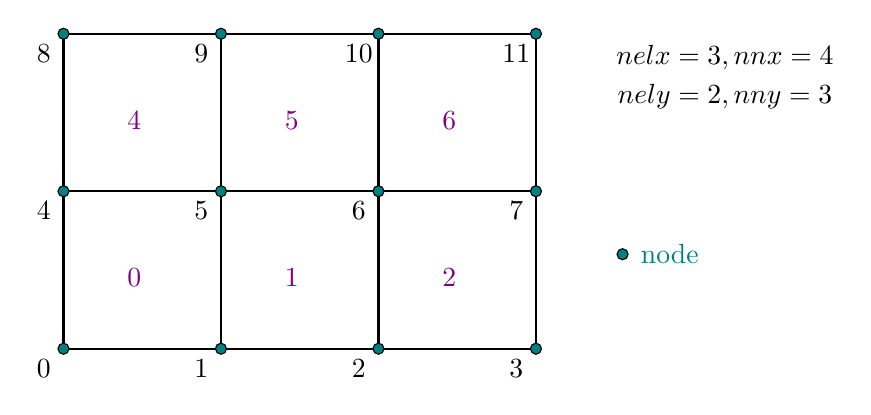
\begin{tikzpicture}
%\draw[step=0.5cm,gray,very thin] (0,0) grid (9,5); %background grid

\draw[thick] (1,1) -- (7,1) -- (7,5) -- (1,5) -- cycle;  
\draw[thick] (1,3) -- (7,3) ;
\draw[thick] (3,1) -- (3,5) ;
\draw[thick] (5,1) -- (5,5) ;

\draw[black,fill=teal] (1,1)     circle (2pt); 
\draw[black,fill=teal] (3,1)     circle (2pt); 
\draw[black,fill=teal] (5,1)     circle (2pt); 
\draw[black,fill=teal] (7,1)     circle (2pt); 

\draw[black,fill=teal] (1,3)     circle (2pt); 
\draw[black,fill=teal] (3,3)     circle (2pt); 
\draw[black,fill=teal] (5,3)     circle (2pt); 
\draw[black,fill=teal] (7,3)     circle (2pt); 

\draw[black,fill=teal] (1,5)     circle (2pt); 
\draw[black,fill=teal] (3,5)     circle (2pt); 
\draw[black,fill=teal] (5,5)     circle (2pt); 
\draw[black,fill=teal] (7,5)     circle (2pt); 

\node[] at (0.75,0.75) {0};
\node[] at (2.75,0.75) {1};
\node[] at (4.75,0.75) {2};
\node[] at (6.75,0.75) {3};

\node[] at (0.75,2.75) {4};
\node[] at (2.75,2.75) {5};
\node[] at (4.75,2.75) {6};
\node[] at (6.75,2.75) {7};

\node[] at (0.75,4.75) {8};
\node[] at (2.75,4.75) {9};
\node[] at (4.75,4.75) {10};
\node[] at (6.75,4.75) {11};

\node[violet] at (1.9,1.9) {0};
\node[violet] at (3.9,1.9) {1};
\node[violet] at (5.9,1.9) {2};
\node[violet] at (1.9,3.9) {4};
\node[violet] at (3.9,3.9) {5};
\node[violet] at (5.9,3.9) {6};

\draw[black,fill=teal] (8.1,2.2) circle (2pt); 
\node[] at (8.7,2.2) {{\color{teal}node}};

\node[] at (9.4,4.7) {$nelx=3, nnx=4$};
\node[] at (9.4,4.2) {$nely=2, nny=3$};

\end{tikzpicture}

\end{center}

\noindent In the case there is only a single degree of freedom per node, the 
assembled FEM matrix ${\bm M}$ will look like this:
\[
{\bm M}=
\left(
\begin{array}{cccccccccccc}
\Box & \Box &      &      & \Box & \Box &      &      &      &      &      &      \\
\Box & \Box & \Box &      & \Box & \Box & \Box &      &      &      &      &      \\
     & \Box & \Box & \Box &      & \Box & \Box & \Box &      &      &      &      \\
     &      & \Box & \Box &      &      & \Box & \Box &      &      &      &      \\
\Box & \Box &      &      & \Box & \Box &      &      & \Box & \Box &      &      \\
\Box & \Box & \Box &      & \Box & \Box & \Box &      & \Box & \Box & \Box &      \\
     & \Box & \Box & \Box &      & \Box & \Box & \Box &      & \Box & \Box & \Box \\
     &      & \Box & \Box &      &      & \Box & \Box &      &      & \Box & \Box \\
     &      &      &      & \Box & \Box &      &      & \Box & \Box &      &      \\
     &      &      &      & \Box & \Box & \Box &      & \Box & \Box & \Box &      \\
     &      &      &      &      & \Box & \Box & \Box &      & \Box & \Box & \Box \\
     &      &      &      &      &      & \Box & \Box &      &      & \Box & \Box 
\end{array}
\right)
\]
where the $\Box$ stand for non-zero terms.
This matrix structure stems from the fact that
\begin{itemize}
\item node 0 sees nodes 0,1,4,5 (1st line/column of the matrix)
\item node 1 sees nodes 0,1,2,4,5,6 (2nd line/column of the matrix)
\item node 2 sees nodes 1,2,3,5,6,7 (3rd line/column of the matrix)
\item node 3 sees nodes 2,3,6,7
\item node 4 sees nodes 0,1,4,5,8,9
\item node 5 sees nodes 0,1,2,4,5,6,8,9,10 
\item node 6 sees nodes 1,2,3,5,6,7,9,10,11
\item node 7 sees nodes 2,3,6,7,10,11
\item node 8 sees nodes 4,5,8,9
\item node 9 sees nodes 4,5,6,8,9,10
\item node 10 sees nodes 5,6,7,9,10,11 
\item node 11 sees nodes 6,7,10,11 (last line/column of the matrix)
\end{itemize}
In light thereof, we have
\begin{itemize}
\item 4 corner nodes which have 4 neighbours (counting themselves) 
\item 2(nnx-2) nodes which have 6 neighbours
\item 2(nny-2) nodes which have 6 neighbours
\item (nnx-2)$\times$(nny-2) nodes which have 9 neighbours
\end{itemize}
In total, the number of non-zero terms in the matrix above is then:
\[
NZ=4\times4+4\times6+2\times6+2\times9=70
\]
and in general, we would then have:
\[
NZ=4\times4+[2(nnx-2)+2(nny-2)]\times6 + (nnx-2)(nny-2)\times9
\]
Let us temporarily assume $nnx=nny=n$. The matrix size (total
number of unknowns) is then $N=n^2$ and  
\[
NZ=16+24(n-2)+9(n-2)^2
\]
A full matrix array would contain $N^2=n^4$ terms. 
The ratio of $NZ$ (the actual number of reals to store)
to the full matrix size (the number of reals a full matrix contains) is then 
\[
R = \frac{16+24(n-2)+9(n-2)^2}{n^4}
\]
It is then obvious that when $n$ is large enough $R \sim 1/n^2$.

CSR stores the nonzeros of the matrix row by row, in a
single indexed array A of double precision  numbers.
Another array COLIND contains the column index of each
corresponding entry in the A array. A third integer array RWPTR
contains pointers to the beginning of each row, which an additional pointer to
the first index following the nonzeros of the matrix A.
A and COLIND have length NZ and RWPTR has length N+1.

In the case of the here-above matrix, the arrays COLIND and RWPTR will look like:
\begin{eqnarray}
COLIND&=&(0,1,4,5, \; 0,1,2,4,5,6, \; 1,2,3,5,6,7, ..., 6,7,10,11) \nn\\
RWPTR &=&(0,4,10,16, ... )   \nn
\end{eqnarray}

%..............................................................................
\subsubsection{2D domain - Symmetric matrix CSR storage}

If the matrix is symmetric, i.e. ${\bm M}={\bm M}^T$, then we may wish to 
only store half of it, always in the interest of saving memory. 
Only the following remaining $\Box$ entries are relevant now:
\[
{\bm M}=
\left(
\begin{array}{cccccccccccc}
\Box & \Box &      &      & \Box & \Box &      &      &      &      &      &      \\
     & \Box & \Box &      & \Box & \Box & \Box &      &      &      &      &      \\
     &      & \Box & \Box &      & \Box & \Box & \Box &      &      &      &      \\
     &      &      & \Box &      &      & \Box & \Box &      &      &      &      \\
     &      &      &      & \Box & \Box &      &      & \Box & \Box &      &      \\
     &      &      &      &      & \Box & \Box &      & \Box & \Box & \Box &      \\
     &      &      &      &      &      & \Box & \Box &      & \Box & \Box & \Box \\
     &      &      &      &      &      &      & \Box &      &      & \Box & \Box \\
     &      &      &      &      &      &      &      & \Box & \Box &      &      \\
     &      &      &      &      &      &      &      &      & \Box & \Box &      \\
     &      &      &      &      &      &      &      &      &      & \Box & \Box \\
     &      &      &      &      &      &      &      &      &      &      & \Box 
\end{array}
\right)
\]
We see that the number of nonzeros is now 
\[
NZ_{symm}= \frac{NZ-n}{2}+n
\]
and in this case $NZ_{symm}=(70-12)/2+12=41$.
Then 
\begin{eqnarray}
COLIND&=&(0,1,4,5, \; 1,2,4,5,6, \; 3,5,6,7, ..., ,11) \nn\\
RWPTR &=&(0,4,9,14, ... )   \nn
\end{eqnarray}


%..............................................................................
\subsubsection{2D domain - Two degrees of freedom per node}

When there are now two degrees of freedom per node, such as in the case of the Stokes equation
in two-dimensions, the size of the $\K$ matrix is given $NfemV=nnx*nny*ndofV$  
where $NfemV$ is the total number of velocity degrees of freedom.

\begin{center}
\begin{flushright} {\tiny {\color{gray} (tikz\_3x2\_two.tex)}} \end{flushright}
%~~~~~~~~~~~~~~~~~~~~~~~~~~~~~~~~~~~~~~~~~~~~~~~~~~~~~~~~~~~~~~~~~~~~~~~~~~~~~~~~~~~~~~~~~~~~~~~~~~


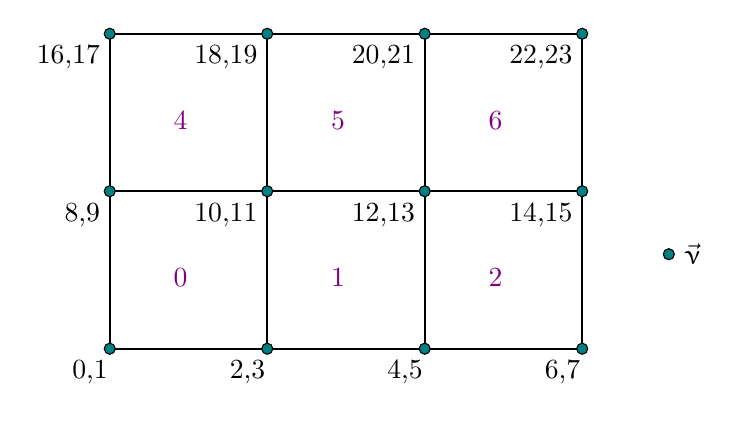
\begin{tikzpicture}
%\draw[step=0.5cm,gray,very thin] (0,0) grid (5,5); %background grid

\draw[thick] (1,1) -- (7,1) -- (7,5) -- (1,5) -- cycle;  
\draw[thick] (1,3) -- (7,3) ;
\draw[thick] (3,1) -- (3,5) ;
\draw[thick] (5,1) -- (5,5) ;

\draw[black,fill=teal] (1,1)     circle (2pt); 
\draw[black,fill=teal] (3,1)     circle (2pt); 
\draw[black,fill=teal] (5,1)     circle (2pt); 
\draw[black,fill=teal] (7,1)     circle (2pt); 

\draw[black,fill=teal] (1,3)     circle (2pt); 
\draw[black,fill=teal] (3,3)     circle (2pt); 
\draw[black,fill=teal] (5,3)     circle (2pt); 
\draw[black,fill=teal] (7,3)     circle (2pt); 

\draw[black,fill=teal] (1,5)     circle (2pt); 
\draw[black,fill=teal] (3,5)     circle (2pt); 
\draw[black,fill=teal] (5,5)     circle (2pt); 
\draw[black,fill=teal] (7,5)     circle (2pt); 

\node[] at (0.75,0.7) {0,1};
\node[] at (2.75,0.7) {2,3};
\node[] at (4.75,0.7) {4,5};
\node[] at (6.75,0.7) {6,7};

\node[] at (0.65,2.7) {8,9};
\node[] at (2.475,2.7) {10,11};
\node[] at (4.475,2.7) {12,13};
\node[] at (6.475,2.7) {14,15};

\node[] at (0.475,4.7) {16,17};
\node[] at (2.475,4.7) {18,19};
\node[] at (4.475,4.7) {20,21};
\node[] at (6.475,4.7) {22,23};

\node[violet] at (1.9,1.9) {0};
\node[violet] at (3.9,1.9) {1};
\node[violet] at (5.9,1.9) {2};
\node[violet] at (1.9,3.9) {4};
\node[violet] at (3.9,3.9) {5};
\node[violet] at (5.9,3.9) {6};

\draw[black,fill=teal] (8.1,2.2) circle (2pt); 
\node[] at (8.4,2.2) {$\vec\upnu$};

\end{tikzpicture}





\end{center}

In the case of the small grid above, we have then $NfemV=24$ and
elemental matrices are now $8\times8$ in size.

We still have
\begin{itemize}
\item $4$ corner nodes which have 4 neighbours
\item $2(nnx-2)$ nodes which have 6 neighbours
\item $2(nny-2)$ nodes which have 6 neighbours
\item $(nnx-2)\cdot(nny-2)$ nodes which have 9 neighbours,
\end{itemize}
but now each degree of freedom from a node sees the other two
degrees of freedom of another node too.
In that case, the number of nonzeros has been multiplied by four
and the assembled FEM matrix looks like:
\begin{equation}
\left(
\begin{array}{cccccccccccccccccccccccc}
\Box&\Box & \Box&\Box &  &  &  &  & \Box&\Box & \Box&\Box &  &  &  &  &  &  &  &  &  &  &  &  \\
\Box&\Box & \Box&\Box &  &  &  &  & \Box&\Box & \Box&\Box &  &  &  &  &  &  &  &  &  &  &  &  \\
\Box&\Box & \Box&\Box & \Box&\Box &  &  & \Box&\Box & \Box&\Box & \Box&\Box &  &  &  &  &  &  &  &  &  &  \\
\Box&\Box & \Box&\Box & \Box&\Box &  &  & \Box&\Box & \Box&\Box & \Box&\Box &  &  &  &  &  &  &  &  &  &  \\
 &  & \Box&\Box & \Box&\Box & \Box&\Box &  &  & \Box&\Box & \Box&\Box & \Box&\Box &  &  &  &  &  &  &  &  \\
 &  & \Box&\Box & \Box&\Box & \Box&\Box &  &  & \Box&\Box & \Box&\Box & \Box&\Box &  &  &  &  &  &  &  &  \\
 &  &  &  & \Box&\Box & \Box&\Box &  &  &  &  & \Box&\Box & \Box&\Box &  &  &  &  &  &  &  &  \\
 &  &  &  & \Box&\Box & \Box&\Box &  &  &  &  & \Box&\Box & \Box&\Box &  &  &  &  &  &  &  &  \\
\Box&\Box & \Box&\Box &  &  &  &  & \Box&\Box & \Box&\Box &  &  &  &  & \Box&\Box & \Box&\Box &  &  &  &  \\
\Box&\Box & \Box&\Box &  &  &  &  & \Box&\Box & \Box&\Box &  &  &  &  & \Box&\Box & \Box&\Box &  &  &  &  \\
\Box&\Box & \Box&\Box & \Box&\Box &  &  & \Box&\Box & \Box&\Box & \Box&\Box &  &  & \Box&\Box & \Box&\Box & \Box&\Box &  &  \\
\Box&\Box & \Box&\Box & \Box&\Box &  &  & \Box&\Box & \Box&\Box & \Box&\Box &  &  & \Box&\Box & \Box&\Box & \Box&\Box &  &  \\
 &  & \Box&\Box & \Box&\Box & \Box&\Box &  &  & \Box&\Box & \Box&\Box & \Box&\Box &  &  & \Box&\Box & \Box&\Box & \Box&\Box \\
 &  & \Box&\Box & \Box&\Box & \Box&\Box &  &  & \Box&\Box & \Box&\Box & \Box&\Box &  &  & \Box&\Box & \Box&\Box & \Box&\Box \\
 &  &  &  & \Box&\Box & \Box&\Box &  &  &  &  & \Box&\Box & \Box&\Box &  &  &  &  & \Box&\Box & \Box&\Box \\
 &  &  &  & \Box&\Box & \Box&\Box &  &  &  &  & \Box&\Box & \Box&\Box &  &  &  &  & \Box&\Box & \Box&\Box \\
 &  &  &  &  &  &  &  & \Box&\Box & \Box&\Box &  &  &  &  & \Box&\Box & \Box&\Box &  &  &  &  \\
 &  &  &  &  &  &  &  & \Box&\Box & \Box&\Box &  &  &  &  & \Box&\Box & \Box&\Box &  &  &  &  \\
 &  &  &  &  &  &  &  & \Box&\Box & \Box&\Box & \Box&\Box &  &  & \Box&\Box & \Box&\Box & \Box&\Box &  &  \\
 &  &  &  &  &  &  &  & \Box&\Box & \Box&\Box & \Box&\Box &  &  & \Box&\Box & \Box&\Box & \Box&\Box &  &  \\
 &  &  &  &  &  &  &  &  &  & \Box&\Box & \Box&\Box & \Box&\Box &  &  & \Box&\Box & \Box&\Box & \Box&\Box \\
 &  &  &  &  &  &  &  &  &  & \Box&\Box & \Box&\Box & \Box&\Box &  &  & \Box&\Box & \Box&\Box & \Box&\Box \\
 &  &  &  &  &  &  &  &  &  &  &  & \Box&\Box & \Box&\Box &  &  &  &  & \Box&\Box & \Box&\Box \\
 &  &  &  &  &  &  &  &  &  &  &  & \Box&\Box & \Box&\Box &  &  &  &  & \Box&\Box & \Box&\Box 
\end{array}
\right)\nonumber
\end{equation}
Note that the degrees of freedom are organised as follows: 
\[
(u_0,v_0,u_1,v_1,u_2,v_2, ... u_{11},v_{11})
\]
In general, we would then have:
\[
NZ=4 \left[4\times4+[2(nnx-2)+2(nny-2)]\times6 + (nnx-2)(nny-2)\times9 \right]
\]
and in the case of the small grid,
the number of non-zero terms in the matrix is then:
\[
NZ=4\left[4\times4+4\times6+2\times6+2\times9\right]=280
\]
In the case of the here-above matrix, the arrays COLIND and RWPTR will look like:
\begin{eqnarray}
COLIND&=&(0,1,2,3,8,9,10,11, \; 0,1,2,3,8,9,10,11,\; ...) \nn\\
RWPTR &=&(0,8,16,28, ... ) \nn
\end{eqnarray}


%..............................................................................
\subsubsection{3D domain - CSR- Three degrees of freedom}


Let us consider a $3\times4\times2$ grid which counts 
$nnx\cdot nny \cdot nnz = 5 \cdot 4\cdot 3=60$ nodes.
The assembled FEM matrix $\K$ size is then 
$N=nnx\times nny\times nnz \times ndof=180$.

\begin{center}
\begin{flushright} {\tiny {\color{gray} (tikz\_4x3x2.tex)}} \end{flushright}
%~~~~~~~~~~~~~~~~~~~~~~~~~~~~~~~~~~~~~~~~~~~~~~~~~~~~~~~~~~~~~~~~~~~~~~~~~~~~~~~~~~~~~~~~~~~~~~~~~~


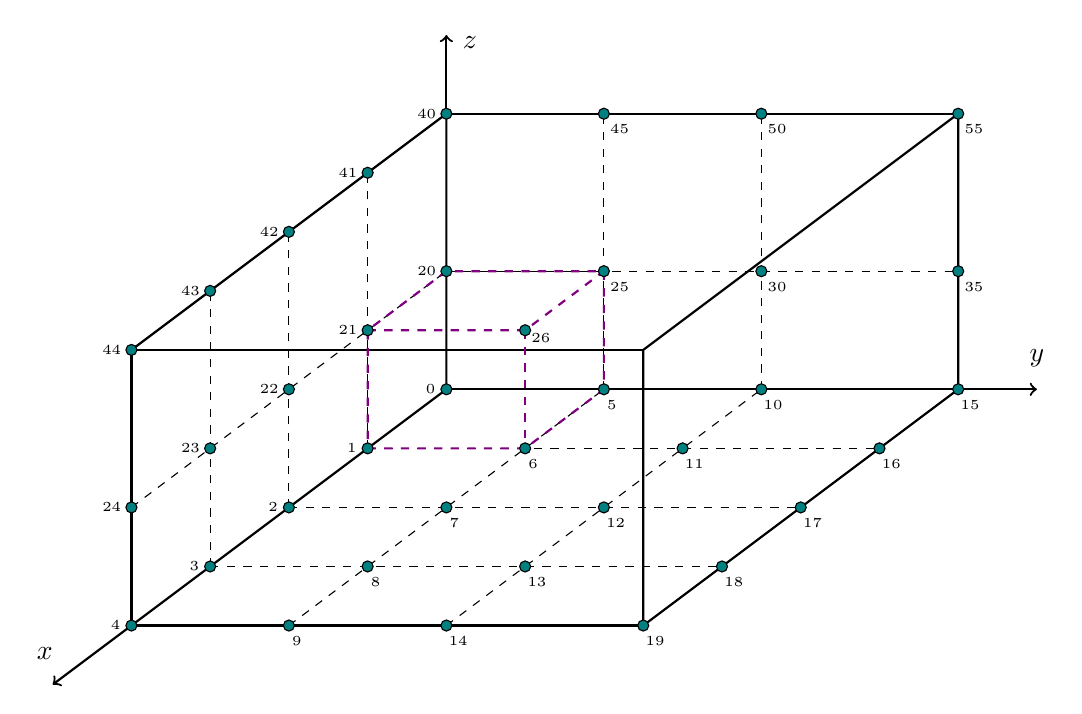
\begin{tikzpicture}
%\draw[step=0.5cm,gray,very thin] (0,0) grid (14,10); %background grid

%element
\draw[thick] (2,2) -- (8.5,2) -- (8.5,5.5) -- (2,5.5) -- cycle;  
\draw[thick] (2,2) -- (6,5) -- (6,8.5) -- (2,5.5) -- cycle ;
\draw[thick] (8.5,2) -- (12.5,5) -- (12.5,8.5) -- (8.5,5.5) -- cycle ;
\draw[thick] (6,5) -- (12.5,5) ;
\draw[thick] (6,8.5) -- (12.5,8.5) ;

%axes
\draw[thick,->] (2,2)--(1,1.25);
\draw[thick,->] (12.5,5)--(13.5,5);
\draw[thick,->] (6,8.5)--(6,9.5);
\node[] at (0.9,1.65) {$x$};
\node[] at (13.5,5.4) {$y$};
\node[] at (6.3,9.4) {$z$};

\draw[dashed] (2,3.5)--(6,6.5);
\draw[dashed] (3,2.75)--(3,6.25);
\draw[dashed] (4,3.5)--(4,7);
\draw[dashed] (5,4.25)--(5,7.75);
\draw[dashed] (4,2)--(8,5);
\draw[dashed] (6,2)--(10,5);
\draw[dashed] (3,2.75)--(9.5,2.75);
\draw[dashed] (4,3.5)--(10.5,3.5);
\draw[dashed] (5,4.25)--(11.5,4.25);
\draw[dashed] (6,6.5)--(12.5,6.5);
\draw[dashed] (8,5)--(8,8.5);
\draw[dashed] (10,5)--(10,8.5);

\draw[dashed, thick,violet] (5,4.25)--(7,4.25) --(8,5)--(8,6.5) --(6,6.5)--(5,5.75)--(5,4.25);
\draw[dashed, thick,violet] (5,5.75)--(7,5.75)--(8,6.5);
\draw[dashed, thick,violet] (7,5.75)--(7,4.25);

\draw[black,fill=teal] (2,2) circle (2pt); 
\draw[black,fill=teal] (3,2.75) circle (2pt); 
\draw[black,fill=teal] (4,3.5) circle (2pt); 
\draw[black,fill=teal] (5,4.25) circle (2pt); 
\draw[black,fill=teal] (6,5) circle (2pt); 

\draw[black,fill=teal] (2,3.5) circle (2pt); 
\draw[black,fill=teal] (3,4.25) circle (2pt); 
\draw[black,fill=teal] (4,5) circle (2pt); 
\draw[black,fill=teal] (5,5.75) circle (2pt); 
\draw[black,fill=teal] (6,6.5) circle (2pt); 

\draw[black,fill=teal] (2,5.5) circle (2pt); 
\draw[black,fill=teal] (3,6.25) circle (2pt); 
\draw[black,fill=teal] (4,7) circle (2pt); 
\draw[black,fill=teal] (5,7.75) circle (2pt); 
\draw[black,fill=teal] (6,8.5) circle (2pt); 

\draw[black,fill=teal] (4,2) circle (2pt); 
\draw[black,fill=teal] (5,2.75) circle (2pt); 
\draw[black,fill=teal] (6,3.5) circle (2pt); 
\draw[black,fill=teal] (7,4.25) circle (2pt); 
\draw[black,fill=teal] (8,5) circle (2pt); 

\draw[black,fill=teal] (6,2) circle (2pt); 
\draw[black,fill=teal] (7,2.75) circle (2pt); 
\draw[black,fill=teal] (8,3.5) circle (2pt); 
\draw[black,fill=teal] (9,4.25) circle (2pt); 
\draw[black,fill=teal] (10,5) circle (2pt); 

\draw[black,fill=teal] (8.5,2) circle (2pt); 
\draw[black,fill=teal] (9.5,2.75) circle (2pt); 
\draw[black,fill=teal] (10.5,3.5) circle (2pt); 
\draw[black,fill=teal] (11.5,4.25) circle (2pt); 
\draw[black,fill=teal] (12.5,5) circle (2pt);

\draw[black,fill=teal] (7,5.75) circle (2pt);


\draw[black,fill=teal] (8,6.5) circle (2pt);
\draw[black,fill=teal] (8,8.5) circle (2pt);

\draw[black,fill=teal] (10,6.5) circle (2pt);
\draw[black,fill=teal] (10,8.5) circle (2pt);

\draw[black,fill=teal] (12.5,6.5) circle (2pt);
\draw[black,fill=teal] (12.5,8.5) circle (2pt);

\node[] at (5.8,5) {\tiny 0};
\node[] at (4.8,4.25) {\tiny 1};
\node[] at (3.8,3.5) {\tiny 2};
\node[] at (2.8,2.75) {\tiny 3};
\node[] at (1.8,2) {\tiny 4};

\node[] at (5.75,6.5) {\tiny 20};
\node[] at (4.75,5.75) {\tiny 21};
\node[] at (3.75,5) {\tiny 22};
\node[] at (2.75,4.25) {\tiny 23};
\node[] at (1.75,3.5) {\tiny 24};

\node[] at (5.75,8.5) {\tiny 40};
\node[] at (4.75,7.75) {\tiny 41};
\node[] at (3.75,7) {\tiny 42};
\node[] at (2.75,6.25) {\tiny 43};
\node[] at (1.75,5.5) {\tiny 44};

\node[] at (8.1,4.8) {\tiny 5};
\node[] at (7.1,4.05) {\tiny 6};
\node[] at (6.1,3.3) {\tiny 7};
\node[] at (5.1,2.55) {\tiny 8};
\node[] at (4.1,1.8) {\tiny 9};

\node[] at (10.15,4.8) {\tiny 10};
\node[] at (9.15,4.05) {\tiny 11};
\node[] at (8.15,3.3) {\tiny 12};
\node[] at (7.15,2.55) {\tiny 13};
\node[] at (6.15,1.8) {\tiny 14};

\node[] at (12.65,4.8) {\tiny 15};
\node[] at (11.65,4.05) {\tiny 16};
\node[] at (10.65,3.3) {\tiny 17};
\node[] at (9.65,2.55) {\tiny 18};
\node[] at (8.65,1.8) {\tiny 19};

\node[] at (8.2,6.3) {\tiny 25};
\node[] at (7.2,5.65) {\tiny 26};

\node[] at (8.2,8.3) {\tiny 45};
\node[] at (10.2,6.3) {\tiny 30};
\node[] at (10.2,8.3) {\tiny 50};

\node[] at (12.7,6.3) {\tiny 35};
\node[] at (12.7,8.3) {\tiny 55};

\end{tikzpicture}

\end{center}



The total number of nonzeros in the case $ndof=1$ would be decomposed as follows:
\begin{itemize}
\item 8 corners 'see' 8 neighbours
\item 4 edges with $(nnx-2)$ nodes in the x direction see 12 nodes
\item 4 edges with $(nny-2)$ nodes in the y direction see 12 nodes
\item 4 edges with $(nnz-2)$ nodes in the z direction see 12 nodes
\item $2(nnx-2)(nny-2)$ nodes see 18 nodes
\item $2(nnx-2)(nnz-2)$ nodes see 18 nodes
\item $2(nny-2)(nnz-2)$ nodes see 18 nodes
\item $(nnx-2)(nny-2)(nnz-2)$ interior nodes see 27 nodes
\end{itemize}





%..............................................................................
\subsubsection{Matrix Storage in fieldstone}

The majority of the codes have the FE matrix being a full array
\begin{lstlisting}
a_mat = np.zeros((Nfem,Nfem),dtype=np.float64) 
\end{lstlisting}
and it is converted to CSR format on the fly in the solve phase:
\begin{lstlisting}
sol = sps.linalg.spsolve(sps.csr_matrix(a_mat),rhs)
\end{lstlisting}

Note that linked list storages can be used (lil\_matrix). Substantial memory savings 
but much longer compute times since it takes longer to write in such arrays.
A conversion to CSR format is still necessary before calling the solver.




%..............................................................................
\subsubsection{Sparse Matrix-Vector multiplication}
\index{general}{SpMV} \index{general}{Sparse Matrix-Vector Multiplication}

When/if the matrix ${\bm M}$ is stored in a two-dimensional array, 
its (left or right) multiplication by a vector is trivial. 
Either one resorts to writing a double for loop (not recommended), 
either one uses {\tt numpy.dot}\footnote{\url{https://numpy.org/doc/stable/reference/generated/numpy.dot.html}}
in python, or {\tt matmul} in Fortran.

However, when the matrix is stored as a single continuous array, say CSR, how does this work?
This question is {\it very important} since iterative solvers such as the Conjugate Gradient solver
(see Section~\ref{ss:itsolvers}) rely extensively on multiplying the matrix by many different vectors. 

The Sparse Matrix-Vector multiplication operation is often abbreviated SpMV.
To quote Knepley \cite{knepley}: "The Sparse Matrix-Vector Product (SpMV) is today 
a workhorse of scientific computing. It is a central kernel is iterative linear and 
nonlinear solvers for PDE, and now for many graph algorithms."
As explained in Williams \etal (2007) \cite{wiov07} (and in many 
other sources on the topic), the algorithm for 
a basic SpMV implementation is rather simple in its naive form. 

\begin{center}
\includegraphics[width=17cm]{images/spmv/widc08}\\
{\captionfont Taken from Williams \etal (2008) \cite{widc08}. 
Sparse Matrix Vector Multiplication (SpMV). 
(a) visualization of the algebra: $\vec{y} \leftarrow {\bm A}\cdot \vec{x}$.\\
(b) Standard compressed sparse row (CSR) representation of the matrix.  \\
(c) The standard implementation of SpMV for a matrix stored in CSR. 
The outer loop is trivially parallelized without any data dependencies.}
\end{center}

Let us assume that we wish to compute $\vec{y}={\bm A}\cdot \vec{x}$ where ${\bm A}$ 
is in CSR format. The pseudo code then goes as follows:
\begin{verbatim}
for i in range(0,m):
    y0=0
    for k in range(ROWPTR[i],ROWPTR[i+1]):
        y0 += VAL[k] * x[COLIND[k]]
    y[i]=y0
\end{verbatim} 
Although technically correct, this algorithm is problematic because the vector x array
is accessed indirectly and this causes a non-optimal use of the processor, which 
in the end makes the calculation take longer than it should.


The following piece of code comes from \elefant. Note that here (ROWPTR=ia, COLIND=ja, VAL=mat)
\begin{lstlisting}[language=Fortran]
subroutine spmv (nr,nc,nz,x,y,mat,ja,ia)
implicit none
integer, intent(in)  :: nr,nc,nz
real(8), intent(in)  :: x(nc), mat(nz)
real(8), intent(out) :: y(nr)
integer, intent(in)  :: ja(nz),ia(nr+1)
real(8) t
integer i, k

do i = 1,nr
   t = 0.0d0
   do k=ia(i), ia(i+1)-1
      t = t + mat(k)*x(ja(k))
   end do
   y(i) = t 
end do

end subroutine
\end{lstlisting}


How to make this calculation as efficiently as possible on CPUs and GPUs, on one thread 
or multiple threads has given rise to a lot of literature.

\Literature Krotkiewski \& Dabrowski \cite{krda10}, Section 9.4 of Kepley \cite{knepley}, 
Williams \etal (2008) \cite{widc08}

 %---------------------------------------------
\newpage %-----------------------------------------------------------------------------------------
\subsection{Mesh generation} \label{subsection_meshes} \begin{flushright} {\tiny {\color{gray} meshes.tex}} \end{flushright}
%~~~~~~~~~~~~~~~~~~~~~~~~~~~~~~~~~~~~~~~~~~~~~~~~~~~~~~~~~~~~~~~~~~~~~~~~~~~~~~~~~~~~~~~~~~~~~~~~~~

Before basis functions can be defined and PDEs can be discretised and solved 
we must first tesselate the domain with polygons, e.g. triangles and 
quadrilaterals in 2D, tetrahedra, prisms and hexahedra in 3D. \index{general}{Convex Polygon} 

When the domain is itself simple (e.g. a rectangle, a sphere, ...) the mesh (or grid) can 
be (more or less) easily produced and the connectivity array filled with straightforward 
algorithms \cite{thie18}.
However, real life applications can involve extremely complex geometries (e.g. a bridge, 
a human spine, a car chassis and body, etc ...) and dedicated algorithms/softwares 
must be used (see \cite{thsw,frge,xiyz09}). 

We usually distinguish between two broad classes of grids: structured grids (with a regular 
connectivity) and unstructured grids (with an irregular connectivity).
\index{general}{Structured Grid} \index{general}{Unstructured Grid}

\begin{center}
\includegraphics[width=5cm]{images/meshes/structured_grid}
\includegraphics[width=5cm]{images/meshes/unstructured_grid}
\end{center}

\begin{remark}
\index{general}{Meshless}
Various families of so-called meshless methods exist and are commonly employed in Computational 
Fluid Dynamics \cite{liugu,liliu,grliu,liuliu}. They are however very rarely used in 
Computational geodynamics, with a noticeable exception \cite{hans03}.
\end{remark}

%............................................
\subsubsection{Quadrilateral-based meshes}

Let us now focus on the case of a rectangular computational domain of size 
{\tt Lx} $\times$ {\tt Ly} with a regular mesh composed of {\tt nelx}$\times${\tt nely}={\tt nel}
   quadrilaterals.  
There are then {\tt nnx}$\times${\tt nny}={\tt nnp} grid points.
The elements are of size {\tt hx}$\times${\tt hy} with {\tt hx}={\tt Lx}/{\tt nelx}.

We have no reason to come up with an irregular/illogical node numbering so 
we can number nodes row by row or column by column as shown on the example 
hereunder of a 3$\times$2 grid:

\begin{verbatim}
8=======9======10======11       2=======5=======8======11
|       |       |       |       |       |       |       |
|  (3)  |  (4)  |  (5)  |       |  (1)  |  (3)  |  (5)  |
|       |       |       |       |       |       |       |
4=======5=======6=======7       1=======4=======7======10
|       |       |       |       |       |       |       |
|  (0)  |  (1)  |  (2)  |       |  (0)  |  (2)  |  (4)  |
|       |       |       |       |       |       |       |
0=======1=======2=======3       0=======3=======6=======9

     "row by row"                  "column by column"
\end{verbatim}

The numbering of the elements themselves could be done in a somewhat chaotic 
way but we follow the numbering of the nodes for simplicity.
The row by row option is the adopted one in \fieldstone{} and the coordinates of the 
points are computed as follows:

\begin{lstlisting}
x = np.empty(nnp, dtype=np.float64)
y = np.empty(nnp, dtype=np.float64)
counter = 0
for j in range(0,nny):
    for i in range(0,nnx):
        x[counter]=i*hx
        y[counter]=j*hy
        counter += 1
\end{lstlisting}
The inner loop has {\tt i} ranging from {\tt 0} to {\tt nnx-1} first for {\tt j}=0, 1, ...
up to {\tt nny-1} which indeed corresponds to the row by row numbering.

\index{general}{Connectivity Array} 
We now turn to the connectivity. As mentioned before, this is a structured mesh so that the so-called
connectivity array, named {\tt icon} in our case, can be filled easily. For each element we need
to store the node identities of its vertices. Since there are {\tt nel} elements and {\tt m=4} corners, 
this is a {\tt m}$\times${\tt nel} array. The algorithm goes as follows:

\begin{lstlisting}
icon =np.zeros((m,nel),dtype=np.int16)
counter = 0
for j in range(0,nely):
    for i in range(0,nelx):
        icon[0,counter] = i + j * nnx 
        icon[1,counter] = i + 1 + j * nnx 
        icon[2,counter] = i + 1 + (j + 1) * nnx 
        icon[3,counter] = i + (j + 1) * nnx 
        counter += 1
\end{lstlisting}

In the case of the 3$\times$2 mesh, the {\tt icon} is filled as follows:
\begin{center}
\begin{tabular}{ccccccc}
element id$\rightarrow$ &0 &1&2&3&4&5 \\
node id$\downarrow$ \\
0& 0& 1& 2& 4& 5  &6\\
1& 1& 2& 3& 5& 6  &7\\
2& 5& 6& 7& 9& 10 &11\\
3& 4& 5& 6& 8& 9  &10\\
\end{tabular}
\end{center}
It is to be understood as follows: element $\#4$ is composed of nodes 5, 6, 10 and 9.
Note that nodes are always stored in a counter clockwise manner, starting at the bottom left.
This is very important since the corresponding basis functions and their derivatives 
will be labelled accordingly.

In three dimensions things are very similar. The mesh now counts 
{\tt nelx}$\times${\tt nely}$\times${\tt nelz}={\tt nel} elements which represent 
a cuboid of size {\tt Lx}$\times${\tt Ly}$\times${\tt Lz}.
The position of the nodes is obtained as follows:
\begin{lstlisting}
x = np.empty(nnp,dtype=np.float64)
y = np.empty(nnp,dtype=np.float64)
z = np.empty(nnp,dtype=np.float64)
counter=0
for i in range(0,nnx):
    for j in range(0,nny):
        for k in range(0,nnz):
            x[counter]=i*hx
            y[counter]=j*hy
            z[counter]=k*hz
            counter += 1
\end{lstlisting}
The connectivity array is now of size {\tt m}$\times${\tt nel} with {\tt m=8}:
\begin{lstlisting}
icon =np.zeros((m,nel),dtype=np.int16)
counter = 0
for i in range(0,nelx):
    for j in range(0,nely):
        for k in range(0,nelz):
            icon[0,counter]=nny*nnz*(i  )+nnz*(j  )+k
            icon[1,counter]=nny*nnz*(i+1)+nnz*(j  )+k
            icon[2,counter]=nny*nnz*(i+1)+nnz*(j+1)+k
            icon[3,counter]=nny*nnz*(i  )+nnz*(j+1)+k
            icon[4,counter]=nny*nnz*(i  )+nnz*(j  )+k+1
            icon[5,counter]=nny*nnz*(i+1)+nnz*(j  )+k+1
            icon[6,counter]=nny*nnz*(i+1)+nnz*(j+1)+k+1
            icon[7,counter]=nny*nnz*(i  )+nnz*(j+1)+k+1
            counter += 1
\end{lstlisting}

\improvement[inline]{produce drawing of node numbering}

Although it is not very common in geosciences, quadrilateral meshes are sometimes 
employed in a boundary-fitted way, as shown hereunder:

\begin{center}
\includegraphics[width=7cm]{images/meshes/gukt16}\\
\end{center}


\Literature: \cite{jole97}

%...................................................
\subsubsection{Delaunay triangulation and Voronoi cells, and triangle-based meshes}

The topic of Delaunay\footnote{The triangulation is named after 
Boris Delaunay for his work on this topic from 1934.}
 triangulation is vast, but a simple definition can be written 
as follows:
"a Delaunay triangulation for a set P 
of points in a plane is a triangulation DT(P) such that no point in P is  
inside the circumcircle of any triangle in DT(P)." [wikipedia]
Other properties of such triangulations are that they 
maximize the minimum angle of all the angles of the 
triangles in the triangulation.
Note that for four or more 
points on the same circle (e.g., the vertices of a rectangle) the Delaunay triangulation is  
not unique and that points on a line also cannot yield a valid triangulation
(for the simple reason that they do not form a triangle).

\begin{center}
\includegraphics[width=4cm]{images/meshes/delaunay}
\includegraphics[width=4cm]{images/meshes/delaunay3}\\
{\captionfont a) A Delaunay triangulation in the plane with circumcircles shown.
b) The Delaunay triangulation of a random set of 100 points in a plane.}
\end{center}

The Delaunay triangulation of a discrete point set P in general corresponds 
to the dual graph of the Voronoi diagram for P. 
A Voronoi diagram is composed of non-overlapping Voronoi cells which make a partition 
of the plane. 
For each point there is a corresponding region consisting of all points closer to that 
point than to any other: this region is the Voronoi cell of that point.

\begin{center}
a)\includegraphics[width=4cm]{images/meshes/delaunay2}
b)\includegraphics[width=4cm]{images/meshes/voronoi}\\
{\captionfont a) The Delaunay triangulation with all the circumcircles and their centers (in red).
b) Connecting the centers of the circumcircles produces the Voronoi diagram (in red). }
\end{center}

The Delaunay triangulation is used in the \douar code which is based on a particle levelset function to track materials. These particles are connected by means of a Delaunay triangulation (usually in a plane at startup, and then in a local Euclidean geometry once the surface is deformed) \cite{brtf08}.

\Literature: \cite{gebo}.


Once a Delaunay triangulation has been obtained it can be used as a FEM mesh.  
Triangle-based meshes are obviously better suited for simulations of complex geometries:
\begin{center}
\includegraphics[height=4cm]{images/meshes/tr1}
\includegraphics[height=4cm]{images/meshes/dolfin}\\
\includegraphics[height=3.8cm]{images/meshes/gebk12}\cite{gebk12}
\includegraphics[height=3.8cm]{images/meshes/rost05a}\cite{rost05a}
\end{center}

A very practical 2D triangle mesher is the 
code {\sl Triangle}\footnote{\url{https://www.cs.cmu.edu/~quake/triangle.html}}
written by J.R. Shewchuk \cite{shew96,shew02,shew14}.
Triangle is specialized for creating two-dimensional finite element meshes, but can 
also perform simpler related tasks such as forming Delaunay triangulations under various assumptions.
Another very common mesher tool is Gmsh \cite{gere09}.

\begin{center}
\includegraphics[width=13cm]{images/meshes/bugw01}\\
{\captionfont Taken from Buiter \etal \cite{bugw01}. Finite element grid. 
The subducting plate initially extends to 1226 km in the horizontal direction and 
is not completely shown here. Discretization in the subducting plate is slightly coarser 
towards the right edge.}
\end{center}

\begin{center}
\includegraphics[width=13cm]{images/meshes/bafl16}\\
{\captionfont Numerical model setup of the 2D axisymmetric half-space with all applied 
boundary conditions to study the effects of ice-cap unloading
on shallow volcanic systems \cite{bafl16}}
\end{center}

\begin{center}
\includegraphics[width=13cm]{images/meshes/fegh14}\\
{\captionfont Taken from \cite{fegh14}. Modelling of slow
landslides. Finite element mesh in the initial and excavated configuration.}
\end{center}

Although it is rarely used in practice it is possible to produce meshes which contain 
both quadrilateral and triangular elements:
\begin{center}
\includegraphics[width=13cm]{images/meshes/fige95}\\
{\captionfont Mesh used to analayse the stress distribution around a pressurized crack in a layered 
elastic medium \cite{fige95}}
\end{center}

\Literature \fullcite{musd15}\fullcite{vemm09}

\begin{remark} 
The Natural Neighbour Interpolation method of Sambridge \etal \cite{sabm95,sabm96} is based on the Delaunay triangulation.
\end{remark}

\begin{remark} 
Moresi \& Mather \cite{moma19} have released Stripy, a A Python module for (constrained) triangulation
in Cartesian coordinates and on a sphere, which is based on Stripack \cite{renk96,renk97}.
\end{remark}

\todo[inline]{write about gmesh}

\begin{center}
\includegraphics[width=6cm]{images/meshes/gusa98a}
\includegraphics[width=6cm]{images/meshes/gusa98b}\\
{\captionfont Taken from Gudmundsson \& Sambridge (1998) \cite{gusa98}.
Boundaries of Voronoi cells around 4100 of the original 16,200 2x2 degree cells
selected to sample the details of the regionalization.}
\end{center}


%...........................
\subsubsection{Tetrahedra}

\begin{center}
\includegraphics[width=5cm]{images/meshes/glacier}
\includegraphics[width=10cm]{images/meshes/gowo05}\\
{\captionfont Left: Example of 3D mesh \cite{yash15}.
Right: Normalized velocities of a STEP subduction model \cite{gowo05}.}
\end{center}


\begin{center}
\includegraphics[width=7cm]{images/meshes/guyr16}
\includegraphics[width=8cm]{images/meshes/tokv09}\\
{\captionfont Left: 3D finite element grid in Damintun area, including prescribed faults. Guo \etal, 2016 \cite{guyr16}.
Right: Structural reactivation in plate tectonics controlled by olivine crystal anisotropy \cite{tokv09}.}
\end{center}



\begin{center}
\includegraphics[width=6cm]{images/meshes/paml14b}
\includegraphics[width=6.3cm]{images/meshes/codh08}\\
{\captionfont Left: Mesh used for the three-dimensional model. A high resolution mesh is used in
the wedge and subslab domains, while the mesh resolution decays to lower values
toward the edge of the model. All elements are quadratic, allowing for twice the
resolution visualized here. Paczkowski \etal (2014) \cite{paml14b}.
Right: Mid-Ocean Ridge Hydrothermal System: 3D mesh consisting of 2.5m tetrahedron elements. 
Resolution is refined toward the axial center, with the finest resolution between the dashed
lines, and colors indicate computational domains assigned to separate processors.
Coumou \etal (2008) \cite{codh08}.}
\end{center}

Check TetGen mesher \fullcite{si15}. 

%............................................
\subsubsection{Hexahedra}

A hexahedron is a convex polytope isomorphic to the cube $[0,1]^3$.
Edges are line segments, facets are strictly {\bf planar} convex polygons.

\begin{center}
\includegraphics[width=5cm]{images/meshes/hexa.jpg}
\includegraphics[width=6cm]{images/meshes/hexa2}
\end{center}

\Literature Efficient Volume computation for Three- Dimensional hexahedral Cells \cite{duko88,gran97}

%.......................................
\subsubsection{Adaptive Mesh Refinement}
\index{general}{AMR} \index{general}{Adaptive Mesh Refinement}

Let us do a simple calculation and assume we wish to model mantle convection on Earth. 
The inner radius is $R_1=$3485km and the bottom of the lithosphere is at $R_2=$6250km. 
The volume of fluid is then 
\[
V = \frac{4}{3}\pi (R_2^3-R_1^3) \simeq 8.5\times 10^{11} \text{km}^3
\]
Let us further assume that we are satisfied with an average resolution of 10km. 
Each element/cell is then $10^3\text{km}^3$ and the total number of elements/cell is then 
\[
N \simeq 8.5 \times 10^8 \sim {\cal O}(10^9)
\]
This is a very large number. The resulting linear systems from the discretisation of the 
equations on such a mesh will be very even larger for the Stokes equations and solving 
these systems will require very large numbers of CPUs and long compute times. 

Aside from these considerations it is quite obvious that a high resolution mesh is not needed 
in parts of the mantle where large scale upwellings and downwellings occur, but 
probably even higher resolution will be needed in the vicinity of thin plumes and boundary layers. 
This means that a uniform mesh is a sub-optimal way of discretising space for such problems. 

The same reasoning also holds in the lithosphere where for instance narrow plate boundaries need to 
be adequately resolved while the inside of rigid plates can be modelled with coarser meshes. 

Finally, although one could employ meshing software to arrive at well balanced meshes in space, the 
dynamic character of the geodynamics modelling renders this approach cumbersome. A subduction zone, 
a mid-ocean rift or an ascending plume will evolve in time and the mesh will have to evolve in time too. 

In light of all this, it was only a matter of time before Adaptive Mesh Refinement was adopted 
in computatinal geodynamics. However, since the use and update of such meshes is somewhat 
complex in terms of numerical algorithms, its introduction came somewhat late (00's and later).
The \douar code (see Section~\ref{app:codes}) developed originally by J. Braun and Ph. Fullsack 
is a prime example of an early multi-purpose code relying on a self-written Octree library \cite{brtf08}.
More recently the \aspect{} code was developed on top of the Octree library p4est \cite{buwg11}

For further reading I suggest you read the review by May, Schellart \& Moresi on this topic \cite{masm13}.

\begin{center}
\includegraphics[height=6cm]{images/meshes/bugg08.jpg}
\includegraphics[height=6cm]{images/meshes/bugg10.jpg}\\
{\captionfont Taken from \cite{bugg08} and \cite{bugg10}}
\end{center}

\begin{center}
\includegraphics[height=3.8cm]{images/meshes/gltf18.jpg}\\
{\captionfont Taken from \cite{gltf18}}
\end{center}


\Literature: \cite{bugg08,bugg10}\cite{lezh11} \cite[sect 3]{bugs09} \cite{dadh07}
\cite{svna18} \cite{mish11}


\newpage
\paragraph{A short illustrative exercise}.


\noindent 
\includegraphics[width=4.5cm]{images/meshes/AMR/amr0}
\includegraphics[width=4.5cm]{images/meshes/AMR/amr1}
\includegraphics[width=4.5cm]{images/meshes/AMR/amr2}\\
\includegraphics[width=4.5cm]{images/meshes/AMR/amr3}
\includegraphics[width=4.5cm]{images/meshes/AMR/amr4}
\includegraphics[width=4.5cm]{images/meshes/AMR/amr5}\\
\includegraphics[width=4.5cm]{images/meshes/AMR/amr6}
\includegraphics[width=4.5cm]{images/meshes/AMR/amr7}
\includegraphics[width=4.5cm]{images/meshes/AMR/amr8}

\begin{tabular}{l|ccccccccc}
             & \# l0  & \# l1 & \# l2 & \# l3 & \# l4 & \# l5 & \# l6 & \# l7 & \# l8 \\ 
\hline\hline
max level= 0 & 1 & \\
max level= 1 & 0 & 4 & \\
max level= 2 & 0 & 3 & 4 \\
max level= 3 & 0 & 2 & 7 & 4\\
max level= 4 & 0 & 2 & 5 & 10 & 8 \\
max level= 5 & 0 & 1 & 8 & 12 & 11 & 20 \\ 
max level= 6 & 0 & 1 & 8 & 11 & 13 & 20 & 32 \\
max level= 7 & 0 & 0 & 11 & 14 & 15 & 23 & 37 & 60 \\
max level= 8 & 0 & 0 & 11 & 13 & 17 & 27 & 43 & 72 & 116 \\
\hline
\end{tabular}

\includegraphics[width=7.28cm]{images/meshes/AMR/amr_data1.pdf}
\includegraphics[width=7.28cm]{images/meshes/AMR/amr_data2.pdf}

In the particular case presented here, even though the inclusion in a short 
two-dimensional line, the total number of elements grows faster than the 
third power of the refinement level. While of course the total number 
of elements remains much smaller than the constant resolution counterpart, 
this observation tells us that authorising a unit increase of the maximum 
refinement level can have a substantial effect on the total number of elements.

\newpage

\noindent
\includegraphics[width=4cm]{images/meshes/AMR/amr_0}
\includegraphics[width=4cm]{images/meshes/AMR/amr_1}
\includegraphics[width=4cm]{images/meshes/AMR/amr_2}
\includegraphics[width=4cm]{images/meshes/AMR/amr_3}\\
\includegraphics[width=4cm]{images/meshes/AMR/amr_4}
\includegraphics[width=4cm]{images/meshes/AMR/amr_5}
\includegraphics[width=4cm]{images/meshes/AMR/amr_6}
\includegraphics[width=4cm]{images/meshes/AMR/amr_7}


\includegraphics[width=5cm]{images/meshes/AMR/amr_data3.pdf}
\includegraphics[width=5cm]{images/meshes/AMR/amr_data4.pdf}
\includegraphics[width=5cm]{images/meshes/AMR/amr_data5.pdf}






%.......................................
\subsubsection{Conformal Mesh Refinement \label{ss:cmr}}
\index{general}{Conformal Mesh Refinement}

The quadtree/octree mesh refinement presented above is one option
when it comes to mesh refinement (or $h$-refinement). However their 
massive drawback is the presence of hanging notes which require 
special attention. 
Another approach to mesh refinement is conformal mesh refinement
as best exemplified on the following figures: 

\begin{center}
\includegraphics[height=4.5cm]{images/meshes/amrnew}\\
{\captionfont Taken from Deb \etal (1996) \cite{depl96}.
A typical instance of the outcome of the refinement procedure. 
Notice that the `spill-over' is reduced to one row on each side of the `localized' elements.}
\end{center}

\begin{center}
\includegraphics[height=4.5cm]{images/meshes/vaks15}
\includegraphics[height=4.5cm]{images/meshes/depl96}
\includegraphics[height=4.5cm]{images/meshes/habo04}\\
\includegraphics[height=4.5cm]{images/meshes/kott05}
\includegraphics[height=4.5cm]{images/meshes/specfem}\\
\includegraphics[height=4.5cm]{images/meshes/conf3D}\\
{\captionfont 
Top row, From left to right: 
van Driel \etal (2015) \cite{vaks15}; 
Deb \etal (1996) \cite{depl96}; 
Harris \etal (2004) \cite{habo04}; 
Komatitsch \etal (2005) \cite{kott05}; 
Middle row: Specfem manual;
Bottom row: I don't know anymore.}
\end{center}

\begin{center}
\includegraphics[height=5cm]{images/meshes/gari09_a}
\includegraphics[height=5cm]{images/meshes/gari09_b}\\
{\captionfont Taken from Garimella (2009) \cite{gari09}.}
\end{center}

\begin{center}
\includegraphics[height=4cm]{images/meshes/newmeshref1}
\includegraphics[height=4cm]{images/meshes/newmeshref2}
\end{center}


\begin{center}
\includegraphics[height=4cm]{images/meshes/refine_mesh_sheet_directional1}
\includegraphics[height=4cm]{images/meshes/refine_mesh_sheet_directional2}
\includegraphics[height=4cm]{images/meshes/refine_mesh_sheet_directional4}\\
\url{https://cubit.sandia.gov/public/14.0/help_manual/WebHelp/mesh_generation/mesh_modification/mesh_refinement.htm}
\end{center}

\Literature: 
D{\"u}ster \& Rank \cite{dura01},
Harris \etal (2004) \cite{habo04},
Anderson \etal (2009) \cite{anbo09},
Anderson \cite{ande09}, 
Garimella (2009) \cite{gari09},
Nicolas \& Fouquet (2013) \cite{nifo13,nifo13b}.
Parrish \cite{parr07}, 
Schneiders \cite{schn00,schn96,schn96b,schn99},
Schneiders \etal \cite{scde95},
Staten \& Canann \cite{stca97},
book by Ramm \etal \cite{rarr03}.


%.......................................
\subsubsection{Stretching the mesh}

In some cases the topology of the mesh can be regular but one can for instance stretch 
the mesh such that (for instance) the vertical resolution is higher at the top than at the bottom, 
or higher in the middle than on the sides.

The idea behind the transformation is a piecewise-linear function which maps [0,L] to [0,L] where 
$L$ is the length of the domain in the $x$-direction. For instance, this transformation can take the following form:

\begin{center}
\includegraphics[width=8cm]{images/meshes/stretching/stretch_towards_center}\\
{\captionfont Parameters $\beta_1$ and $\beta_2$ control the shape of the lines.\\ 
The kinks in the line occur at $\beta_1 L$ and $(1-\beta_1)L$ (see code here under).}
\end{center}

The (minimal) code to transform the mesh is as follows:
\begin{lstlisting}
def stretch_towards_center(x,L,beta1,beta2):
    if x<beta1*L: 
       val = beta2/beta1*x
    elif x<(1.-beta1)*L: 
       val = (1-2*beta2)/(1-2*beta1)*(x-beta1*L)+beta2*L
    else:
       val=beta2/beta1*(x-(1-beta1)*L)+(1-beta2)*L
    return val

[...]

beta1=0.25
beta2=0.375

for i in range(0,NV):
    x[i]=stretch_towards_center(x[i],Lx,beta1,beta2)
\end{lstlisting}

The following meshes count 64x16 elements. The top one is a regular mesh, with square elements, 
while the second one has been stretched by means of the transformation above:

\begin{center}
\includegraphics[width=8cm]{images/meshes/stretching/stretch_x}
\end{center}

Concerning the stretching towards the top of the model domain, the transformation line is as follows:

\begin{center}
\includegraphics[width=8cm]{images/meshes/stretching/stretch_towards_top}\\
{\captionfont Parameters $\beta_1$ and $\beta_2$ control the shape of the lines. The kinks in the 
line occur at $\beta_1 L$ and $(1-\beta_1)L$.\\ The slope of the left line is $\beta_2/\beta_1 x$.}
\end{center}

The (minimal) code to transform the mesh is as follows:
\begin{lstlisting}
def stretch_towards_top(x,L,beta1,beta2):
    if x<beta1*L: 
       val=beta2/beta1*x
    else:
       val=(1-beta2)/(1-beta1)*(x-beta1*L)+beta2*L
    return val

[...]

beta1=0.25
beta2=0.5
for i in range(0,NV):
    y[i]=stretch_towards_top(y[i],Ly,beta1,beta2)
\end{lstlisting}


The following meshes count 64x16 elements. The top one is a regular mesh, with square elements, 
while the second one has been stretched by means of the transformation above.
\begin{center}
\includegraphics[width=8cm]{images/meshes/stretching/stretch_y}
\end{center}

Finally both transformations can be applied to the same mesh:
\begin{center}
\includegraphics[width=8cm]{images/meshes/stretching/stretch_xy}
\end{center}

This approach is used in \stone 67.

%.......................................
\subsubsection{Meshes in an annulus}


\begin{center}
\includegraphics[width=6.8cm]{images/meshes/brhv08}
\includegraphics[width=6.8cm]{images/meshes/brva07a}\\
{\captionfont The quadratic finite element mesh as used in 
Brandenburg \etal \cite{brhv08,brva07a}}
\end{center}


%.......................................
\subsubsection{Meshes in a hollow sphere}

The following is for the most part published in Thieulot (2018) \cite{thie18}.

To a first approximation the Earth is a sphere: the Earth's polar diameter is 
about 43 kilometers shorter than its equatorial diameter, a negligible difference of 
about 0.3\%. As a consequence, modelling physical processes 
which take place in the planet require the discretisation of a sphere. 
Furthermore, because core dynamics occur on vastly difference time scales than mantle dynamics, mantle 
modelling usually leaves the core out, thereby requiring simulations to be run on a hollow sphere mesh
(with the noticeable exception of \cite{geyu07}).

Although so-called latitude-longitude grids would seem appealing, 
they suffer from the convergence of meridians at the poles
(resulting in over sampling at poles) and the juxtaposition of triangles 
near the poles and quadrilaterals elsewhere. 
As a consequence more regular, but more complex, grids have been designed 
over the years which tesselate the surface of the 
sphere into triangles or quadrilaterals (sometimes overlapping).
There is the 'cubed sphere' \cite{roip96,heta03,chob05,sthh06,chcc07,brmw10,yiym19},
the Yin-Yang grid \cite{kasa04,yoka04,yoka06,kaks08,tack08,crta14,crta16},
the Yin-Yang-zhong grid \cite{haka16}, the Yin-yang grid of 
Shahnas \& Peltier \cite{shpe15}, the spiral grid \cite{hust08}, 
an icosahedron-based grid \cite{bafr85,tasu01},
or a grid composed of 12 blocks further subdivided into quadrilaterals \cite{zhzm00} 
as used in the CitcomS code.
Note that \cite{oldp12} have also presented a method for generating a numerical 
grid on a spherical surface which 
allows the grid to be based on several different regular polyhedrons (including octahedron, 
cube, icosahedron, and rhombic dodecahedron). 
Ideally, one wishes to generate a mesh that is regular,
i.e. angles between edges/faces as close to $90^\circ$ as possible, 
of approximately similar volumes.


\begin{center}
\includegraphics[width=12cm]{images/meshes/kaks08}\\
{\captionfont Example of Yin-Yang grid. Taken from Kameyama \etal (2008) \cite{kaks08}.}
\end{center}

How such meshes are built is often not discussed in the literature. It is 
a tedious exercise of three-dimensional geometry and it can be time-consuming, especially 
the connectivity array generation. In Thieulot (2018) \cite{thie18} I present an open source 
mesh generator for three hollow sphere meshes: the 'cubed sphere' mesh, the CitcomS mesh and the 
icosahedral mesh:

\begin{itemize}
\item 
The cubed sphere ('HS06'), composed of 6 blocks which 
are themselves subdivided into $N_b \times N_b$ quadrilateral shaped cells  \cite{sado72,roip96,heta03,busa13}.
Four types of cubed spheres meshes have been proposed: the conformal, elliptic, gnomonic and spring types \cite{puli07}:


\begin{center}
\includegraphics[width=6.5cm]{images/meshes/puli07}
\includegraphics[width=8.5cm]{images/meshes/cubed_nair}\\
{\captionfont 
Left: The cubed-sphere grids at $2^\circ$ resolution displaying cells on the sphere,
 the image focuses on the distribution of grid cells near one corner of the grid;
 (a) conformal mapping \cite{rapm96,mcgr96}, (b) the gnomonic grid modified by elliptic solver,
 (c) equiangular gnomonic mapping and (d) the gnomonic grid modified by spring dynamics. \cite{puli07}.
Right: Taken from presentation by R. Nair, see Nair2008.pdf
}
\end{center}

However only gnomonic meshes are considered in Thieulot (2018): these 
are obtained by inscribing a cube within a sphere and expanding to the surface
of the sphere.
The cubed sphere has been used in large-scale mantle convection simulation in conjunction with 
Adaptive Mesh Refinement \cite{algs12,busa13}.  

\begin{center}
\includegraphics[width=4cm]{images/ghost/hs06}
\end{center}



\item 
The CitcomS mesh ('HS12') composed of 12 blocks also subdivided 
into $N_b \times N_b$ quadrilateral shaped cells
\cite{zhzm00,sthh06,zhmt08,arfw14}.
Note that \aspect{} \cite{krhb12,hedg17}, a relatively new code aimed at 
superseeding CitcomS can generate and use 
this type of mesh \cite{thie17} but is not limited to it.

\begin{center}
\includegraphics[width=4cm]{images/ghost/citcom12}
\end{center}


\item The icosahedral mesh ('HS20') composed of 20 triangular blocks \cite{bafr85,baum85} subdivided into triangles, which is 
used in the TERRA code \cite{burb96,burb97,burl98,dadb13}.
\end{itemize}


\begin{center}
\includegraphics[width=8cm]{images/meshes/spherical_choices1}
\includegraphics[width=8cm]{images/meshes/spherical_choices2}\\
{\captionfont source?}
\end{center}



Given the regularity and symmetry of these meshes determining the location of the 
mesh nodes in space is a relatively straightforward task. Building the mesh connectivity in an 
efficient manner is where the difficulty lies.

The approach to building all three meshes is identical:
\begin{enumerate}
\item A reference square or triangle is populated with cells,
parametrised by a level $l$: the square is subdivided into $l\times l$ quadrilaterals while 
the triangle is subdivided into $l^2$ triangles.
\begin{center}
\includegraphics[width=8cm]{images/ghost/f01_basics}\\
{\captionfont Reference square and triangles meshes at level 5.}
\end{center}

\item This reference square or triangle is then replicated {\sl nblock} times (6, 12 or 20) and mapped
onto a portion of a unit sphere. The blocks are such that their union covers a full sphere
but they cannot overlap except at the edges:
\begin{center}
\includegraphics[width=.8\linewidth]{images/ghost/f02}\\
{\captionfont From left to right: HS06, HS12 and HS20 shells coloured by block number.}
\end{center}

\item All block meshes are then merged together to generate a shell mesh. This task is rather 
complex as duplicate nodes must be removed and all connectivity arrays of the blocks must then 
be mended accordingly. 

\item Shell meshes are replicated {\sl nlayer+1} times outwards with increasing radii. 
The {\sl nlayer} shells are then merged together to form a hollow sphere mesh:
\begin{center}
\includegraphics[width=10cm]{images/ghost/f03_3HS}\\
{\captionfont a) HS06 mesh composed of 6 blocks containing each $6^3$ cells; 
b) HS12 mesh composed of 12 blocks containing each 
$6^3$ cells; e) HS20 mesh composed of 20 blocks containing each $6^3$ cells.}
\end{center}

\end{enumerate}



More information on these steps is available in the manual of the code.
In the following table the number of nodes and cells for a variety of resolutions 
for all three mesh types is reported. Looking at the CitcomS literature of the past 20 years, we find that 
the mesh data presented in this table cover the various resolutions used, e.g.
$12\times48^3$ \cite{mczh04,arfw14}, $12\times64^3$ \cite{budt14}
$12\times96^3$ \cite{bumb10}, $12\times128^3$ \cite{beck06,wele16,welm16}.
Note that in the case of the HS06 and HS12 meshes the mesh nodes are mapped out to the 6 or 12 blocks 
following either an equidistant or equiangle approach (see \cite{puli07}
for details on both approaches). 

\begin{center}
\begin{tabular}{lrrrl}
\hline
type & level & $N$ & $N_{el}$ & structure\\
\hline
\hline
HS06 & 
2   &  78        &  48         &$6\times 2^3$    \\
HS06 & 
4   &  490       &  384        &$6\times 4^3$    \\
HS06 & 
8   &  3,474      &  3,072       &$6\times 8^3$    \\
HS06 & 
16  &  26,146     &  24,576      &$6\times 16^3$    \\
HS06 & 
32  &  202,818    &  196,608     &$6\times 32^3$    \\
HS06 & 
64  &  1,597,570   &  1,572,864    &$6\times 64^3$    \\
HS06 & 
128 &  12,681,474  &  12,582,912   &$6\times 128^3$    \\
HS06 & 
256 &  101,057,026 &  100,663,296  &$6\times 256^3$    \\
\hline
HS12 & 2    &          150  &          96  &  $12\times 2^3$ \\
HS12 & 4    &          970  &         768  &  $12\times 4^3$ \\
HS12 & 8    &        6,930  &       6,144  &  $12\times 8^3$ \\
HS12 & 16   &       52,258  &      49,152  &  $12\times 16^3$ \\
HS12 & 32   &      405,570  &     393,216  &  $12\times 32^3$ \\
HS12 & 48   &    1,354,850  &   1,327,104  &  $12\times 48^3$ \\
HS12 & 64   &    3,195,010  &   3,145,728  &  $12\times 64^3$ \\
HS12 & 128  &   25,362,690  &  25,165,824  &  $12\times 128^3$ \\
HS12 & 256  &  202,113,538  & 201,326,592  &  $12\times 256^3$ \\
\hline
HS20 & 
2     &         126  &         160   & $20 \times 2^3$ \\
HS20 & 
4     &         810  &       1,280   & $20 \times 4^3$ \\
HS20 & 
8     &       5,778  &      10,240   & $20 \times 8^3$ \\
HS20 & 
16    &      43,554  &      81,920   & $20 \times 16^3$ \\
HS20 & 
32    &     337,986  &     655,360   & $20 \times 32^3$ \\
HS20 & 
64    &   2,662,530  &   5,242,880   & $20 \times 64^3$ \\
HS20 & 
128   &  21,135,618  &  41,943,040   & $20 \times 128^3$ \\
HS20 & 
256   & 168,428,034  & 335,544,320   & $20 \times 256^3$ \\
\hline
\end{tabular}\\
{\captionfont Number of nodes $N$ and elements/cells $N_{el}$ for the three types of meshes and for various 
levels.\\ HS06: cubed sphere; HS12: CitcomS mesh; HS20: icosahedral mesh.}
\end{center}

There are also many possibilities offered by the use of tetrahedral cells/elements:


\begin{center}
\includegraphics[width=7cm]{images/meshes/oebm09}\\
{\captionfont Grid of a global neo-tectonic SHELLS model coupled to a global mantle
circulation model; colours represent temperatures (red=hot, blue=cold)
at a depth of $200\si{km}$ below the surface. Taken from Oeser \etal (2009) \cite{oebm09}.}
\end{center}


\begin{center}
\includegraphics[width=7cm]{images/meshes/htm}\\
{\captionfont Example of a Hierarchical Triangular Mesh}
\end{center}


\begin{center}
\includegraphics[width=7cm]{images/meshes/bafr85}
\includegraphics[width=7cm]{images/meshes/simj12}\\
{\captionfont \cite{bafr85}, \cite{simj12}}
\end{center}


\Literature: Phillips \etal \cite{phdo19} present an algorithm which builds polyhedral-based grids.





 %----------------------------
\newpage %-----------------------------------------------------------------------------------------
\subsection{Visco-Plasticity} 
\Literature: \cite{mumc03,chpe15,momu06,muso11}





















IMPLEMENTATION of plasticity ... WORK IN PROGRESS

%%%%%%%%%%%%%%%%%%%%%%%%%%%%%%%%%%%%%%%%%%%%%%%%%%%%%%%%%%%%%%%%%%%%%%%%%%%%%%%%%%%%%%%%%%%%%%%%%%%%
\subsubsection{Scalar viscoplasticity}

This formulation is quite easy to implement. It is widely used, e.g. \cite{will92,thfb08,spmw16}, and relies on the assumption that 
a scalar quantity $\eta_p$ (the 'effective plastic viscosity') exists such that the deviatoric stress tensor 
\begin{equation}
{\bm \tau}=2\eta_p \dot{\bm\varepsilon} \label{eqscpl1}
\end{equation}
is bounded by some yield stress value $Y$.
From Eq. (\ref{eqscpl1}) it follows that ${\tau}_{e}= 2\eta_p \dot{\varepsilon}_{e}=Y$ which yields
\begin{mdframed}[backgroundcolor=blue!5]
\[
\eta_p = \frac{Y}{2 \dot{\varepsilon}_{e}}
\]
\end{mdframed}
This approach has also been coined the Viscosity Rescaling Method (VRM) \cite{kacha04}. 
\index{general}{VRM} \index{general}{Viscosity Rescaling Method}

\improvement[inline]{insert here the rederivation 2.1.1 of spmw16}

It is at this stage important to realise that (i) in areas where the strainrate is low, the resulting effective viscosity will be large, and 
(ii) in areas where the strainrate is high, the resulting effective viscosity will be low. This is not without consequences since 
(effective) viscosity contrasts up to 8-10 orders of magnitude have been observed/obtained with this formulation and it makes the FE 
matrix very stiff, leading to (iterative) solver convergence issues.
In order to contain these viscosity contrasts one usually resorts to viscosity limiters $\eta_{min}$ and $\eta_{max}$ such that 
\[
\eta_{min} \leq \eta_p \leq \eta_{max}
\]
Caution must be taken when choosing both values as they may influence the final results.


%-------------------------------------------------
{Work in progress}

\Literature \cite{zico74,zigo74,zico74b,zien75,corm75,zigo75,zihl75,zijo78,vidm82,vidm84,vede84,zivt85,vimd86}
\cite{wasd97,debo88,debo01,hesd02,bewv11,mumg10,leor89,sccm13,desm93,demu92,debo91,shmv16}
\cite{modm01}\cite{baji02}\cite{slde92}\cite{lepo13}
\cite{modm02}\cite{vavd99}\cite{miam13}\cite{huly99}\cite{hugh83}

Note that \cite{vidm82,vidm84,vimd86,zivt85} use the following formulation which they attribute to \cite{zijo78}:
\[
\eta_{eff} = \frac{c + (\dot{\varepsilon}_e / \gamma)^{1/n}}{ \dot{\varepsilon}_e }
\] 
For a perfectly plastic flow law, $\gamma \rightarrow \infty$ and then 
\[
\eta_{eff} = \frac{c}{ \dot{\varepsilon}_e }
\] 
and when when $c=0$ then the effective viscosity is essentially of the power law type.
Also, when $n=1$ the formulation becomes identical to the v-vp formulation (when the max viscosity is infinite) and with $1/\gamma=\eta_{min}$.

fractal distribution of shear bands in \cite{pohp94}



 %--------------------------------------------
\newpage %-----------------------------------------------------------------------------------------
\subsection{Pressure smoothing \label{psmoothing}} 
It has been widely documented that the use of the $Q_1 \times P_0$ element is 
not without problems. Aside from the 
consequences it has on the FE matrix properties, we will here focus on another unavoidable side effect: 
the spurious pressure checkerboard modes. 
\index{general}{Pressure Smoothing} 
\index{general}{Checkerboard mode}

These modes have been thoroughly analysed decades ago, see for instance
Hughes et al (1979)\cite{hulb79}, 
Sani et al (1981) \cite{sagl81a,sagl81b},
Griffiths \& Silvester (1994) \cite{grsi94}.
They can be filtered out(Chen (1995)  \cite{chpc95}) 
or simply smoothed (Lee et al (1979) \cite{legs79}), as we will see later.
Nodes on edges and corners may need special treatment as documented in Sani et al \cite{sagl81a} or
Lee et al (1979) \cite{legs79}.
The list of 8 schemes is not exhaustive with regards to the above mentioned publications. 
There has been considerable amount of work on the topic and this section is 
unfortunately not representing the literature appropriately.

\mscthesis: Get all relevant literature, digest it, implement all variants in fieldstone 12.
 \index{general}{MSc Thesis} 


On the following figure (a,b), pressure fields for the lid driven cavity experiment 
are presented for both an even and un-even number of elements. We see that 
the amplitude of the modes can sometimes be so large that the 'real' pressure signal is 
not visible under the checkerboard and that something as simple as the number of elements in the 
domain can trigger those or not at all.

\begin{center}
a)\includegraphics[width=4cm]{images/checkerboard/p_el}
\includegraphics[width=4cm]{images/checkerboard/p_el_33x33}
b)\includegraphics[width=5cm]{images/checkerboard/press_doneahuerta}
c)\includegraphics[width=7cm]{images/checkerboard/douarpunch}\\
{\captionfont a) element pressure for a 32x32 grid and for a 33x33 grid;\\ 
b) image from \cite[p307]{dohu03} for a manufactured solution;
c) elemental pressure and smoothed pressure for the punch experiment \cite{thfb08}}
\end{center}

%----------------------------------------------------------------------
\paragraph{Scheme 1}.

The easiest post-processing step that can be used (especially when a regular grid is used) 
is explained in Thieulot et al (2008) \cite{thfb08}: "The element-to-node interpolation is performed by
averaging the elemental values from elements common to each node; 
the node-to-element interpolation is performed
by averaging the nodal values element-by-element. This
method is not only very efficient but produces a smoothing
of the pressure that is adapted to the local density of the
octree. Note that these two steps can be repeated until a
satisfying level of smoothness (and diffusion) of the pressure field is attained."


\begin{center}
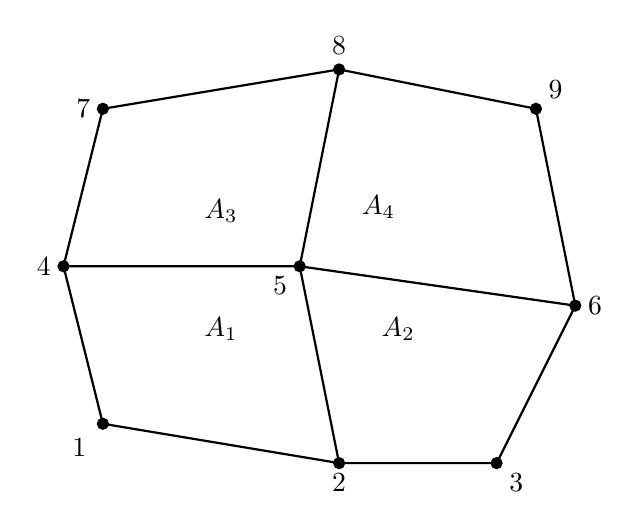
\begin{tikzpicture}
%\draw[fill=gray!5,gray!5](0,0) rectangle (9,7);
%\draw[step=0.5cm,gray,very thin] (0,0) grid (9,7); %background grid
\draw[thick](1.5,1.5) -- (4.5,1) -- (6.5,1) -- (7.5,3) -- (7,5.5) -- (4.5,6) --(1.5,5.5) -- (1,3.5) -- cycle;  
\draw[thick](4.5,1)--(4,3.5)--(4.5,6);
\draw[thick](1,3.5)--(4,3.5)--(7.5,3);
\draw[black,fill=black] (1.5,1.5) circle (2pt); \node[] at (1.2,1.2){1}; %1
\draw[black,fill=black] (4.5,1)   circle (2pt); \node[] at (4.5,0.75){2}; %2
\draw[black,fill=black] (6.5,1)   circle (2pt); \node[] at (6.75,0.75){3}; %3
\draw[black,fill=black] (1,3.5)   circle (2pt); \node[] at (0.75,3.5){4}; %4
\draw[black,fill=black] (4,3.5)   circle (2pt); \node[] at (3.75,3.25){5}; %5
\draw[black,fill=black] (7.5,3)   circle (2pt); \node[] at (7.75,3){6}; %6
\draw[black,fill=black] (1.5,5.5) circle (2pt); \node[] at (1.25,5.5){7}; %7
\draw[black,fill=black] (4.5,6)   circle (2pt); \node[] at (4.5,6.3){8}; %8
\draw[black,fill=black] (7,5.5)   circle (2pt); \node[] at (7.25,5.75){9}; %9
%\draw[thin,dashed](1,3.5)--(4.5,1)--(7.5,3)--(4.5,6)--cycle;
\node[] at (3,2.7){$A_1$}; %8
\node[] at (5.25,2.7){$A_2$}; %8
\node[] at (5,4.25){$A_4$}; %8
\node[] at (3,4.2){$A_3$}; %8
\end{tikzpicture}
\end{center}
\[
q_5^{(1)} = \frac{1}{4}\sum_{e=1}^4 p_e
\] 

In the codes which rely on the $Q_1 \times P_0$ element, the (elemental) pressure
is simply defined as 
\begin{lstlisting}
p=np.zeros(nel,dtype=np.float64)  
\end{lstlisting}
while the nodal pressure is then defined as\footnote{In virtually all stones $p$
stands for the 'raw' pressure and $q$ stands for its projection onto the velocity mesh.} 
\begin{lstlisting}
q=np.zeros(nnp,dtype=np.float64)  
\end{lstlisting}
The element-to-node algorithm is then simply (in 2D):

\begin{lstlisting}
count=np.zeros(nnp,dtype=np.int32)  
for iel in range(0,nel):
    q[icon[0,iel]]+=p[iel]
    q[icon[1,iel]]+=p[iel]
    q[icon[2,iel]]+=p[iel]
    q[icon[3,iel]]+=p[iel]
    count[icon[0,iel]]+=1
    count[icon[1,iel]]+=1
    count[icon[2,iel]]+=1
    count[icon[3,iel]]+=1
q=q/count
\end{lstlisting}



%----------------------------------------------------------------------
\paragraph{Schemes 2,3}.

{\sl Schemes 2,3} are very similar and are presented in Sani et al (1981) \cite{sagl81a,sagl81b}.
Scheme 2 uses the areas of the surrounding elements as weights for the arithmetic averaging
while scheme 3 uses the area of the triangles:

\begin{multicols}{2}

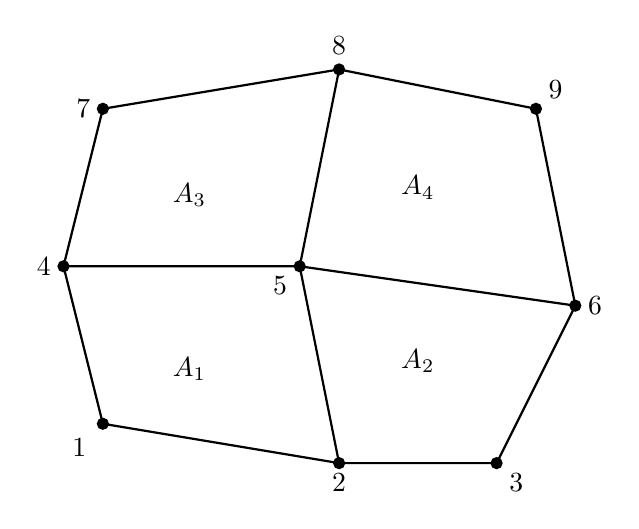
\begin{tikzpicture}
%\draw[fill=gray!5,gray!5](0,0) rectangle (9,7);
%\draw[step=0.5cm,gray,very thin] (0,0) grid (9,7); %background grid
\draw[thick](1.5,1.5) -- (4.5,1) -- (6.5,1) -- (7.5,3) -- (7,5.5) -- (4.5,6) --(1.5,5.5) -- (1,3.5) -- cycle;  
\draw[thick](4.5,1)--(4,3.5)--(4.5,6);
\draw[thick](1,3.5)--(4,3.5)--(7.5,3);
\draw[black,fill=black] (1.5,1.5) circle (2pt); \node[] at (1.2,1.2){1}; %1
\draw[black,fill=black] (4.5,1)   circle (2pt); \node[] at (4.5,0.75){2}; %2
\draw[black,fill=black] (6.5,1)   circle (2pt); \node[] at (6.75,0.75){3}; %3
\draw[black,fill=black] (1,3.5)   circle (2pt); \node[] at (0.75,3.5){4}; %4
\draw[black,fill=black] (4,3.5)   circle (2pt); \node[] at (3.75,3.25){5}; %5
\draw[black,fill=black] (7.5,3)   circle (2pt); \node[] at (7.75,3){6}; %6
\draw[black,fill=black] (1.5,5.5) circle (2pt); \node[] at (1.25,5.5){7}; %7
\draw[black,fill=black] (4.5,6)   circle (2pt); \node[] at (4.5,6.3){8}; %8
\draw[black,fill=black] (7,5.5)   circle (2pt); \node[] at (7.25,5.75){9}; %9
\node[] at (2.6,2.2){$A_1$}; %8
\node[] at (5.5,2.3){$A_2$}; %8
\node[] at (2.6,4.4){$A_3$}; %8
\node[] at (5.5,4.5){$A_4$}; %8
\end{tikzpicture}

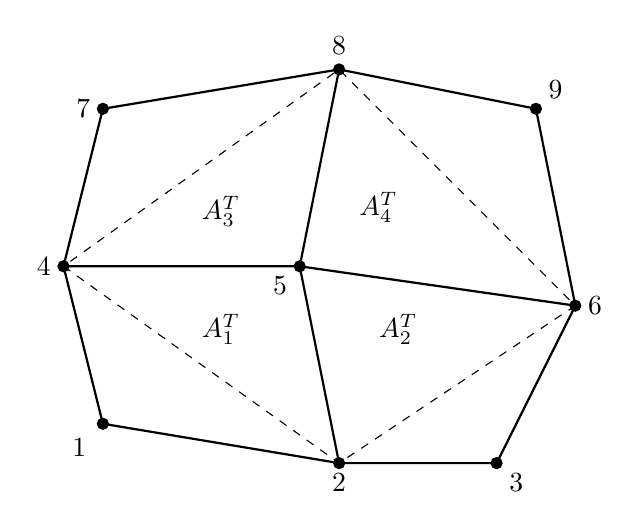
\begin{tikzpicture}
%\draw[fill=gray!5,gray!5](0,0) rectangle (9,7);
%\draw[step=0.5cm,gray,very thin] (0,0) grid (9,7); %background grid
\draw[thick](1.5,1.5) -- (4.5,1) -- (6.5,1) -- (7.5,3) -- (7,5.5) -- (4.5,6) --(1.5,5.5) -- (1,3.5) -- cycle;  
\draw[thick](4.5,1)--(4,3.5)--(4.5,6);
\draw[thick](1,3.5)--(4,3.5)--(7.5,3);
\draw[black,fill=black] (1.5,1.5) circle (2pt); \node[] at (1.2,1.2){1}; %1
\draw[black,fill=black] (4.5,1)   circle (2pt); \node[] at (4.5,0.75){2}; %2
\draw[black,fill=black] (6.5,1)   circle (2pt); \node[] at (6.75,0.75){3}; %3
\draw[black,fill=black] (1,3.5)   circle (2pt); \node[] at (0.75,3.5){4}; %4
\draw[black,fill=black] (4,3.5)   circle (2pt); \node[] at (3.75,3.25){5}; %5
\draw[black,fill=black] (7.5,3)   circle (2pt); \node[] at (7.75,3){6}; %6
\draw[black,fill=black] (1.5,5.5) circle (2pt); \node[] at (1.25,5.5){7}; %7
\draw[black,fill=black] (4.5,6)   circle (2pt); \node[] at (4.5,6.3){8}; %8
\draw[black,fill=black] (7,5.5)   circle (2pt); \node[] at (7.25,5.75){9}; %9
\draw[thin,dashed](1,3.5)--(4.5,1)--(7.5,3)--(4.5,6)--cycle;
\node[] at (3,2.7){$A_1^T$}; %8
\node[] at (5.25,2.7){$A_2^T$}; %8
\node[] at (5,4.25){$A_4^T$}; %8
\node[] at (3,4.2){$A_3^T$}; %8
\end{tikzpicture}

\end{multicols}




\[
q_5^{(2)} = \frac{\sum\limits_{e=1}^4 A_e p_e}{\sum\limits_{e=1}^4 A_e}
\qquad
\qquad
q_5^{(3)} = \frac{\sum\limits_{e=1}^4 A_e^T p_e}{\sum\limits_{e=1}^4 A_e^T}
\] 


\begin{remark} Although Schemes 1,2,3 are similar, scheme 1 is the simplest and fastest
to implement since the areas of neighbouring elements/triangles are not needed.
\end{remark}

\begin{remark} 
Schemes 1,2,3 are identical if all elements are rectangles of identical dimensions.
\end{remark}




%----------------------------------------------------------------------
\paragraph{Scheme 4} This scheme has been designed by me. 
It resembles the last three ones, but the weighing is in this case different.

Let us consider a 1D problem:
\begin{center}
\includegraphics[width=0.5\linewidth]{images/pressure_smoothing/newalgo.png}
\end{center}

Elemental pressures $p_1$ and $p_2$ corresponding to elements 1 and 2 respectively are known at
locations $x_1$ and $x_2$. The two elements have a different size, characterised in this case
by the distances $d_1$ and $d_2$ to their common edge.

The equation of the line passing through points $(x_1,p_1)$ and $(x_2,p_2)$ is 
\[
p(x)=\frac{p_2-p_1}{x_2-x_1}(x-x_1)+p_1
\]
The $x$ coordinate of the common edge is given by $x=x_1+d_1/2$, 
and since $x_2-x_1=(d_1+d_2)/2$, the 
pressure at this location writes:
\[
p(x_M)= \frac{p_2-p_1}{d_1+d_2}d_1+p_1 = \frac{\frac{p_1}{d_1} + \frac{p_2}{d_2}}{\frac{1}{d_1} + \frac{1}{d_2}}
\]
Extrapolating this formula to 2D, $d_1$ and $d_2$ are in fact the element volumes, so that
\[
q_5^{(4)} = 
\frac{\sum\limits_{j=1}^4 \frac{p_j^e}{A_j^e}}{\sum\limits_{j=1}^4 \frac{1}{A_j^e}}
=
\frac{
\frac{p_1^e}{A_1^e}+
\frac{p_2^e}{A_2^e}+
\frac{p_3^e}{A_3^e}+
\frac{p_4^e}{A_4^e}
}{
\frac{1}{A_1^e}+
\frac{1}{A_2^e}+
\frac{1}{A_3^e}+
\frac{1}{A_4^e}
}\]

There remains a problem, due to the presence of the boundary nodes for which 
the sums present in the above equation do not run up to 4. A boundary
node only has three neighbours and a corner node only two. Additional measures
are required for these nodes. 

\begin{center}
\includegraphics[width=0.5\linewidth]{images/pressure_smoothing/newalgo_corner.png}
\end{center}

The pressure value $p_N$ is obtained as follows:
\[
q_N = \frac{ 
 \frac{p_2^e}   {A_2^e}
+\frac{p_3^e}   {A_3^e}
+\frac{p_{2'}^e}{A_{2'}^e}
+\frac{p_{3'}^e}{A_{3'}^e}
}{
 \frac{1}{A_2^e}
+\frac{1}{A_3^e}
+\frac{1}{A_{2'}^e}
+\frac{1}{A_{3'}^e}
}
\]
The areas and pressures of the mirrored elements 2' and 3' are extrapolated from the areas of elements 2 and 6, and 3 and 7 respectively. 
Likewise the pressure $p_M$ at the corner node is obtained through the pressures of its surrounding elements.


%------------------------------------------------------------------------------
\paragraph{Scheme 5 - Least squares} This scheme is presented (among other places) in Lee et al (1979)
\cite{legs79}. 
Let us start from the patch of 4 $Q_1$ elements counting 9 nodes: 

\begin{center}
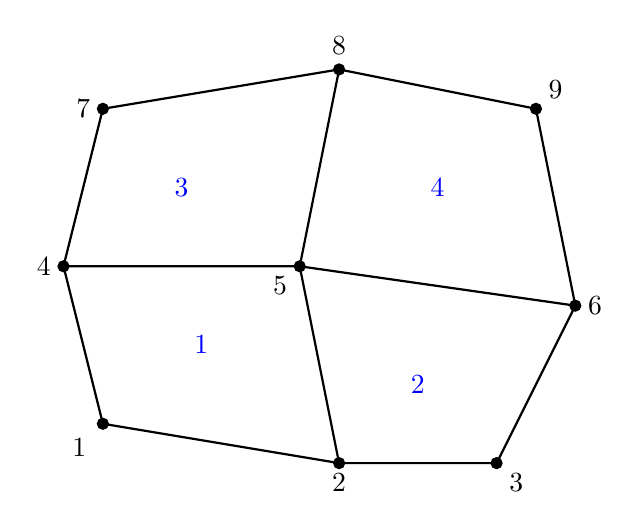
\begin{tikzpicture}
%\draw[fill=gray!5,gray!5](0,0) rectangle (9,7);
%\draw[step=0.5cm,gray,very thin] (0,0) grid (9,7); %background grid
\draw[thick](1.5,1.5) -- (4.5,1) -- (6.5,1) -- (7.5,3) -- (7,5.5) -- (4.5,6) --(1.5,5.5) -- (1,3.5) -- cycle;  
\draw[thick](4.5,1)--(4,3.5)--(4.5,6);
\draw[thick](1,3.5)--(4,3.5)--(7.5,3);

\node[] at (2.75,2.5) {\color{blue}1};
\node[] at (5.5,2) {\color{blue}2};
\node[] at (2.5,4.5) {\color{blue}3};
\node[] at (5.75,4.5) {\color{blue}4};

\draw[black,fill=black] (1.5,1.5) circle (2pt); \node[] at (1.2,1.2){1}; %1
\draw[black,fill=black] (4.5,1)   circle (2pt); \node[] at (4.5,0.75){2}; %2
\draw[black,fill=black] (6.5,1)   circle (2pt); \node[] at (6.75,0.75){3}; %3
\draw[black,fill=black] (1,3.5)   circle (2pt); \node[] at (0.75,3.5){4}; %4
\draw[black,fill=black] (4,3.5)   circle (2pt); \node[] at (3.75,3.25){5}; %5
\draw[black,fill=black] (7.5,3)   circle (2pt); \node[] at (7.75,3){6}; %6
\draw[black,fill=black] (1.5,5.5) circle (2pt); \node[] at (1.25,5.5){7}; %7
\draw[black,fill=black] (4.5,6)   circle (2pt); \node[] at (4.5,6.3){8}; %8
\draw[black,fill=black] (7,5.5)   circle (2pt); \node[] at (7.25,5.75){9}; %9

\end{tikzpicture}
\end{center}



We are looking for a field $q$ living on the nodes.
We build the quantity
\[
J=\iint_\Omega (q-p)^2 dV
\]
where $p$ is the elemental field. To make things clearer we split the integral into 
the sum of elemental integrals:
\[
J=
\iint_{\Omega_1} (q(x,y)-p_1)^2 dV+
\iint_{\Omega_2} (q(x,y)-p_2)^2 dV+
\iint_{\Omega_3} (q(x,y)-p_3)^2 dV+
\iint_{\Omega_4} (q(x,y)-p_4)^2 dV
\]
Inside each element the field $q(x,y)$ is given by a bilinear interpolation so that:
\begin{eqnarray}
J
&=& \iint_{\Omega_1} (N_1(x,y) q_1 + N_2(x,y)q_2 + N_5(x,y)q_5 + N_4(x,y)q_4 -p_1)^2 dV \nn\\
&+& \iint_{\Omega_2} (N_2(x,y) q_2 + N_3(x,y)q_3 + N_6(x,y)q_6 + N_5(x,y)q_5 -p_2)^2 dV \nn\\
&+& \iint_{\Omega_3} (N_4(x,y) q_4 + N_5(x,y)q_5 + N_8(x,y)q_8 + N_7(x,y)q_7 -p_3)^2 dV \nn\\
&+& \iint_{\Omega_4} (N_5(x,y) q_5 + N_6(x,y)q_6 + N_9(x,y)q_9 + N_8(x,y)q_8 -p_4)^2 dV 
\end{eqnarray}
where the $N_i$ functions are the shape functions (unusually expressed in $x,y$ coordinates).
The least square procedure looks for the set of $q_i$ such that 
\[
\frac{\partial J}{\partial q_i} =0 \qquad \forall i=1,...9
\]
and this yields 9 equations/constraints for 9 unknowns.
\begin{eqnarray}
\frac{\partial J}{\partial q_1} 
&=& \iint_{\Omega_1} 2 (N_1(x,y) q_1 + N_2(x,y)q_2 + N_5(x,y)q_5 + N_4(x,y)q_4 -p_1) N_1(x,y) dV \nn\\
\frac{\partial J}{\partial q_2}
&=& \iint_{\Omega_1} 2(N_1(x,y) q_1 + N_2(x,y)q_2 + N_5(x,y)q_5 + N_4(x,y)q_4 -p_1) N_2(x,y) dV \nn\\
&+& \iint_{\Omega_2} 2(N_2(x,y) q_2 + N_3(x,y)q_3 + N_6(x,y)q_6 + N_5(x,y)q_5 -p_2) N_2(x,y) dV \nn\\
\frac{\partial J}{\partial q_3}
&=& \iint_{\Omega_2} 2(N_2(x,y) q_2 + N_3(x,y)q_3 + N_6(x,y)q_6 + N_5(x,y)q_5 -p_2) N_3(x,y) dV \nn\\
\frac{\partial J}{\partial q_4}
&=& \iint_{\Omega_1} 2(N_1(x,y) q_1 + N_2(x,y)q_2 + N_5(x,y)q_5 + N_4(x,y)q_4 -p_1) N_4(x,y) dV \nn\\
&+& \iint_{\Omega_3} 2(N_4(x,y) q_4 + N_5(x,y)q_5 + N_8(x,y)q_8 + N_7(x,y)q_7 -p_3) N_4(x,y) dV \nn\\
\frac{\partial J}{\partial q_5}
&=& \iint_{\Omega_1} 2(N_1(x,y) q_1 + N_2(x,y)q_2 + N_5(x,y)q_5 + N_4(x,y)q_4 -p_1) N_5(x,y) dV \nn\\
&+& \iint_{\Omega_2} 2(N_2(x,y) q_2 + N_3(x,y)q_3 + N_6(x,y)q_6 + N_5(x,y)q_5 -p_2) N_5(x,y) dV \nn\\
&+& \iint_{\Omega_3} 2(N_4(x,y) q_4 + N_5(x,y)q_5 + N_8(x,y)q_8 + N_7(x,y)q_7 -p_3) N_5(x,y) dV \nn\\
&+& \iint_{\Omega_4} 2(N_5(x,y) q_5 + N_6(x,y)q_6 + N_9(x,y)q_9 + N_8(x,y)q_8 -p_4) N_5(x,y) dV \nn\\
\frac{\partial J}{\partial q_6}
&=& \iint_{\Omega_2} 2(N_2(x,y) q_2 + N_3(x,y)q_3 + N_6(x,y)q_6 + N_5(x,y)q_5 -p_2) N_6(x,y) dV \nn\\
&+& \iint_{\Omega_4} 2(N_5(x,y) q_5 + N_6(x,y)q_6 + N_9(x,y)q_9 + N_8(x,y)q_8 -p_4) N_6(x,y) dV \nn\\
\frac{\partial J}{\partial q_7}
&=& \iint_{\Omega_3} 2(N_4(x,y) q_4 + N_5(x,y)q_5 + N_8(x,y)q_8 + N_7(x,y)q_7 -p_3) N_7(x,y) dV \nn\\
\frac{\partial J}{\partial q_8}
&=& \iint_{\Omega_3} 2(N_4(x,y) q_4 + N_5(x,y)q_5 + N_8(x,y)q_8 + N_7(x,y)q_7 -p_3) N_8(x,y)dV \nn\\
&+& \iint_{\Omega_4} 2(N_5(x,y) q_5 + N_6(x,y)q_6 + N_9(x,y)q_9 + N_8(x,y)q_8 -p_4) N_8(x,y)dV \nn\\ 
\frac{\partial J}{\partial q_9}
&=& \iint_{\Omega_4} 2(N_5(x,y) q_5 + N_6(x,y)q_6 + N_9(x,y)q_9 + N_8(x,y)q_8 -p_4) N_9(x,y)dV 
\end{eqnarray}
The factor 2 are removed and the terms $\int p_i N_j $ are known so they end up in the right hand side.

\begin{eqnarray}
 \iint_{\Omega_1} (N_1N_1 q_1 + N_1N_2 q_2 + N_1N_5q_5 + N_1N_4q_4) dV &=& \iint_{\Omega_1} p_1 N_1 dV \nn\\
 \iint_{\Omega_1} (N_2 N_1  q_1 + N_2 N_2q_2 + N_2 N_5q_5 + N_2 N_4q_4)  dV \nn\\
+\iint_{\Omega_2} (N_2 N_2 q_2 + N_3 N_2 q_3 + N_6 N_2 q_6 + N_5 N_2 q_5) dV 
&=& \iint_{\Omega_1} p_1N_2 dV + \iint_{\Omega_2}  p_2 N_2 dV \nn\\
\nn\\
\dots &=& \dots \nn\\
\nn\\
 \iint_{\Omega_4} (N_9N_5 q_5 + N_9N_6q_6 + N_9N_9q_9 + N_9N_8q_8) dV &=&  \iint_{\Omega_4} p_4 N_9 dV 
\end{eqnarray}

The mass matrices corresponding to the four elements are 
\[
{\bm M}_1 = \int_{\Omega_1} \left( \begin{array}{cccc}
N_1 N_1 & N_1 N_2 & N_1 N_5 & N_1 N_4 \\
N_2 N_1 & N_2 N_2 & N_2 N_5 & N_2 N_4 \\
N_5 N_1 & N_5 N_2 & N_5 N_5 & N_5 N_4 \\
N_4 N_1 & N_4 N_2 & N_4 N_5 & N_4 N_4 
\end{array}\right) dV
\qquad
{\bm M}_2 = \int_{\Omega_2} \left( \begin{array}{cccc}
N_2 N_2 & N_2 N_3 & N_2 N_6 & N_2 N_5 \\
N_3 N_2 & N_3 N_3 & N_3 N_6 & N_3 N_5 \\
N_6 N_2 & N_6 N_3 & N_6 N_6 & N_6 N_5 \\
N_5 N_2 & N_5 N_3 & N_5 N_6 & N_5 N_5 
\end{array}\right) dV
\]
\[
{\bm M}_3 = \int_{\Omega_3} \left( \begin{array}{cccc}
N_4 N_4 & N_4 N_5 & N_4 N_8 & N_4 N_7 \\
N_5 N_4 & N_5 N_5 & N_5 N_8 & N_5 N_7 \\
N_8 N_4 & N_8 N_5 & N_8 N_8 & N_8 N_7 \\
N_7 N_4 & N_7 N_5 & N_7 N_8 & N_7 N_7 
\end{array}\right) dV
\qquad
{\bm M}_4 = \int_{\Omega_4} \left( \begin{array}{cccc}
N_5 N_5 & N_5 N_6 & N_5 N_9 & N_5 N_8 \\
N_6 N_5 & N_6 N_6 & N_6 N_9 & N_6 N_8 \\
N_9 N_5 & N_9 N_6 & N_9 N_9 & N_9 N_8 \\
N_8 N_5 & N_8 N_6 & N_8 N_9 & N_8 N_8 
\end{array}\right) dV
\]
so that the 9 equations above are actually the result of the assembly process of these four 
elemental systems:
\[
\left( \iint_{\Omega_e} \vec{N}^T\vec{N} dV \right) \cdot \vec{q}_e = \iint_{\Omega_i} \vec{N}^T p_e dV 
\qquad\qquad e=1,2,3,4
\]


%------------------------------------------------------------------------------
\paragraph{Scheme 6 - Consistent pressure recovery}

The is the method presented in Zienkiewicz \& Nakazawa (1982) \cite{zina82}. In the second part 
of this publication the authors wish to establish a simple and effective numerical method to calculate 
variables eliminated by the penalisation process. 
The method involves an additional finite element solution for the nodal pressures using 
the same finite element basis and numerical quadrature as used for the velocity.

Let us start with\footnote{I here voluntarily use $q$ instead of $p$}:
\[
q = -\lambda \vec\nabla\cdot \vec\upnu
\]
We are going to treat this equation as any other PDE in the context of the FE method, i.e. 
we are going to establish its weak form. 
We assume that the pressure is given inside an element by
\[
q(x,y) = \sum_{i=1}^4 N_i(x,y) q_i = \vec{N} \cdot \vec{q}
\]
and the velocity:
\[
\vec\upnu = (u,v) 
\qquad 
\qquad 
u(x,y)  = \sum_{i=1}^4 N_i(x,y) u_i
\qquad 
\qquad 
v(x,y)  = \sum_{i=1}^4 N_i(x,y) v_i
\]
where the $N_i$ are the $Q_1$ shape functions and $q_i$ are the sought after nodal values. 
We multiply the equation above by a $Q_1$ shape function $N_i$ and integrate over the whole domain:
\[
\iint_\Omega N_i(x,y) q(x,y) \; dxdy = -\lambda \iint_\Omega N_i \vec\nabla\cdot \vec\upnu  \; dx dy
\]
As before we now focus on the above expression inside a single element $e$:
\[
\iint_{\Omega_e} N_i(x,y) q(x,y) \; dxdy = -\lambda \iint_{\Omega_e} N_i \vec\nabla\cdot \vec\upnu \; dx dy
\]
After $N_i \rightarrow \vec{N}=(N_1,N_2,N_3,N_4)^T$, the left hand side term becomes:
\[
\iint _{\Omega_e} \vec{N}^T q(x,y) \; dxdy 
=
\iint _{\Omega_e} \vec{N}^T \vec{N} \cdot \vec{q} \; dxdy 
=
\left(\underbrace{\iint _{\Omega_e} \vec{N}^T \vec{N} dxdy}_{{\bm M}_e} \right) \cdot \vec{q}  
\]
where ${\bm M}_e$ is the elemental mass matrix.
We now turn to the right hand side. We have
\[
\vec\nabla\cdot \vec\upnu
= \frac{\partial u}{\partial x}+\frac{\partial v}{\partial y}
= \sum_i \frac{\partial N_i}{\partial x} u_i + \sum_i \frac{\partial N_i}{\partial y} v_i 
\]
We here too define $\vec{V}_e=(u_1,v_1,u_2,v_2,u_3,v_3,u_4,v_4)^T$ so that 

\begin{eqnarray}
&& \iint_{\Omega_e} \vec{N} {\vec \nabla}\cdot {\vec \upnu} \; d\Omega \nn\\
&=& \iint_{\Omega_e} \vec{N}^T \sum_{i=1}^{4} 
\left( \frac{\partial N_i}{\partial x} u_i + \frac{\partial N_i}{\partial y} v_i 
\right)  
d\Omega \nonumber\\
&=& 
\iint_{\Omega_e} 
\left(
\begin{array}{c}
N_1 \left(
\sum\limits_{i=1}^{4} \frac{\partial N_i}{\partial x} u_i +
\sum\limits_{i=1}^{4} \frac{\partial N_i}{\partial y} v_i \right) \\
N_2 \left(
\sum\limits_{i=1}^{4} \frac{\partial N_i}{\partial x} u_i +
\sum\limits_{i=1}^{4} \frac{\partial N_i}{\partial y} v_i \right) \\
N_3 \left(
\sum\limits_{i=1}^{4} \frac{\partial N_i}{\partial x} u_i +
\sum\limits_{i=1}^{4} \frac{\partial N_i}{\partial y} v_i \right) \\
N_4 \left(
\sum\limits_{i=1}^{4} \frac{\partial N_i}{\partial x} u_i +
\sum\limits_{i=1}^{4} \frac{\partial N_i}{\partial y} v_i \right) 
\end{array}
\right) d \Omega \nonumber \\  %%%%%%%%%%%%%%%%%%%%%%%%%%
&=& 
\int_{\Omega_e} 
\left(
\begin{array}{ccc}
{N}_1& {N}_1 &  0 \\\\
{N}_2& {N}_2 &  0 \\\\
{N}_3& {N}_3 &  0 \\\\
{N}_4& {N}_4 &  0 
\end{array}
\right)
\cdot
\left(
\begin{array}{c}
\sum\limits_i \frac{\partial N_i}{\partial x} u_i \\ \\
\sum\limits_i \frac{\partial N_i}{\partial y} v_i \\ \\
\sum\limits_i (\frac{\partial N_i}{\partial y} u_i\! +\! \frac{\partial N_i}{\partial x} v_i) 
\end{array}
\right)
\; d\Omega \nonumber\\ %%%%%%%%%%%%%%%%%%%%%%%%%%
&=& 
\int_{\Omega_e} 
\underbrace{
\left(
\begin{array}{cccccc}
{N}_1 & {N}_1 &  0 \\
{N}_2 & {N}_2 &  0 \\
{N}_3 & {N}_3 &  0 \\
{N}_4 & {N}_4 &  0 
\end{array}
\right)
}_{{\bm N}}
\cdot
\underbrace{
\left(\begin{array}{cccccccc}
\partial_x N_1 & 0 &  
\partial_x N_2 & 0 &  
\partial_x N_3 & 0 &  
\partial_x N_4 & 0 \\ \\
0 & \partial_y N_1 &   
0 & \partial_y N_2 &   
0 & \partial_y N_3 &   
0 & \partial_y N_4 \\ \\
\partial_y N_1 & \partial_x N_1 &  
\partial_y N_2 & \partial_x N_2 &  
\partial_y N_3 & \partial_x N_3 &  
\partial_y N_4 & \partial_x N_4 
\end{array}\right)}_{{\bm B}}
\cdot \vec{V}_e
\; d\Omega  \nonumber \\
&=& 
\left(\int_{\Omega_e} {\bm N} \cdot {\bm B} \; d\Omega \right) \cdot \vec{V}_e \nonumber\\
&=& -\G_e^T \cdot {\vec V}_e
\end{eqnarray}

After assembly we arrive at
\[
{\bm M} \cdot \vec{q} = \lambda \G^T \cdot {\vec V} 
\qquad
\text{with}
\qquad
\G_e = -\int_{\Omega_e} {\bm N} \cdot {\bm B} \; d\Omega
\]
where ${\bm M}$ is the global mass matrix, $\vec{q}$ the vector of all 
nodal pressures, $\G$ the discrete gradient matrix and $\vec{V}$
the (velocity) solution vector. 
The system can be easily solved since the mass matrix is a friendly matrix.
The vector ${\vec q}$ contains the nodal pressure values directly, with 
no need for a smoothing scheme! 

\begin{remark}
Very importantly, the mass matrix ${\bm M}$ is to be evaluated at the full integration points, 
while the constraint part (the right hand side of the equation) is to be evaluated at 
the reduced integration point, i.e. in the middle of the element.  
\end{remark}

\begin{remark}
As noted in \cite{zina82}, it is interesting to note that when linear elements are used 
and the lumped matrices are used for the ${\bm M}$ the resulting algebraic equation is identical 
to the smoothing scheme 1 only if a uniform square finite element 
mesh is used. In this respect this method is expected to yield different results when elements 
are not square or even rectangular.
\end{remark}

\begin{remark}
The third column of the matrix ${\bm N}$
and the last line of the ${\bm B}$ matrix could be removed altogether.
If your code is based on the mixed formulation, then you already 
have built matrix $\G$ so you can easily re-use this piece of code 
to compute $\G$ again, this time with a reduced integration quadrature.
If you are using the penalty formulation then you need to program 
all from scratch and then simply do away with these unnecessary terms, or 
you can direcly build the rhs as $\int_{\Omega_e} \vec{N}^T p_e$ (assuming
you have previously computed the pressure in the middle of each element 
by means of $p=-\lambda\vec\nabla\cdot\vec\upnu$).
\end{remark}

\begin{remark}
This  scheme is identical to the least square scheme!
\end{remark}


%--------------------------------------------------------------
\paragraph{Scheme 7}

Same as scheme 6, but with lumped mass matrix.  


%--------------------------------------------------------------
\paragraph{Scheme 8 - bilinear interpolation} Let us assume that the centers of the 
four elements make a $Q_1$ quadrilateral element, as shown on this figure:


\begin{center}
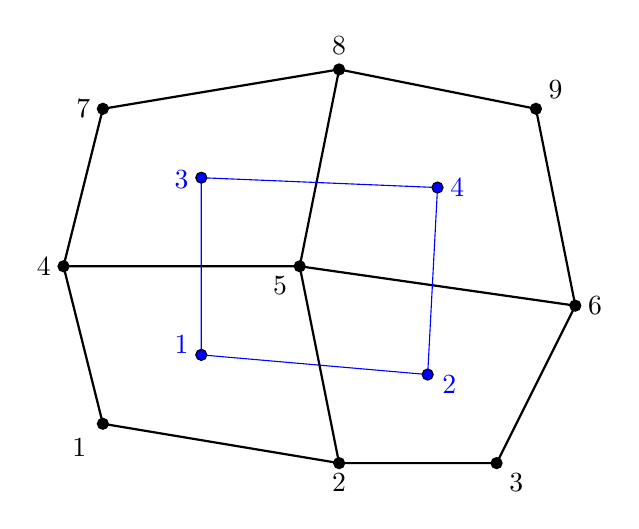
\begin{tikzpicture}
%\draw[fill=gray!5,gray!5](0,0) rectangle (9,7);
%\draw[step=0.5cm,gray,very thin] (0,0) grid (9,7); %background grid
\draw[thick](1.5,1.5) -- (4.5,1) -- (6.5,1) -- (7.5,3) -- (7,5.5) -- (4.5,6) --(1.5,5.5) -- (1,3.5) -- cycle;  
\draw[thick](4.5,1)--(4,3.5)--(4.5,6);
\draw[thick](1,3.5)--(4,3.5)--(7.5,3);

\draw[black,fill=blue] (2.75,2.375) circle (2pt); 
\node[] at (2.5,2.5) {\color{blue}1};
\draw[black,fill=blue] (5.625,2.125) circle (2pt); 
\node[] at (5.9,2) {\color{blue}2};
\draw[black,fill=blue] (5.75,4.5) circle (2pt); 
\node[] at (2.5,4.6) {\color{blue}3};
\draw[black,fill=blue] (2.75,4.625) circle (2pt); 
\node[] at (6,4.5) {\color{blue}4};

\draw[black,fill=black] (1.5,1.5) circle (2pt); \node[] at (1.2,1.2){1}; %1
\draw[black,fill=black] (4.5,1)   circle (2pt); \node[] at (4.5,0.75){2}; %2
\draw[black,fill=black] (6.5,1)   circle (2pt); \node[] at (6.75,0.75){3}; %3
\draw[black,fill=black] (1,3.5)   circle (2pt); \node[] at (0.75,3.5){4}; %4
\draw[black,fill=black] (4,3.5)   circle (2pt); \node[] at (3.75,3.25){5}; %5
\draw[black,fill=black] (7.5,3)   circle (2pt); \node[] at (7.75,3){6}; %6
\draw[black,fill=black] (1.5,5.5) circle (2pt); \node[] at (1.25,5.5){7}; %7
\draw[black,fill=black] (4.5,6)   circle (2pt); \node[] at (4.5,6.3){8}; %8
\draw[black,fill=black] (7,5.5)   circle (2pt); \node[] at (7.25,5.75){9}; %9

\draw[blue](2.75,2.375)--(5.625,2.125)--(5.75,4.5)--(2.75,4.625)--cycle;
\end{tikzpicture}
\end{center}




The values at the corners are $p_1$,
$p_2$, $p_3$ and $p_4$. Assuming that the pressure inside this element can be represented 
by a bilinear field, we have 
\[
p(x,y)= a+ bx +cy +dxy
\]
where the coefficients will be determined by ensuring that $p(x_i,y_i)=p_i$ for $i=1,2,3,4$, or:
\begin{eqnarray}
a+bx_1+cy_1+dx_1y_1 &=& p_1 \\
a+bx_2+cy_2+dx_2y_2 &=& p_2 \\
a+bx_3+cy_3+dx_3y_3 &=& p_3 \\
a+bx_4+cy_4+dx_4y_4 &=& p_4 
\end{eqnarray}
i.e.
\[
\left(
\begin{array}{cccc}
1 & x_1 & y_1 & x_1y_1 \\
1 & x_2 & y_2 & x_2y_2 \\
1 & x_3 & y_3 & x_3y_3 \\
1 & x_4 & y_4 & x_4y_4
\end{array}
\right)\cdot
\left(
\begin{array}{c}
a \\b\\c\\d
\end{array}
\right)
=
\left(
\begin{array}{c}
p_1\\p_2\\p_3\\p_4
\end{array}
\right)
\]

There remains an issue with nodes which are on the boundaries of the domain. These are of course not 
'surrounded' by four pressure values so the above algorithm does not apply directly. However, looking 
at the above figure, and assuming that node 1 is a lower left corner of a 2D domain, we can use the 
bilinear interpolation based on elements 1,2,3,4 to extrapolate a nodal pressure value at node 1. 
The same would apply for nodes 2 and 4 for example. 

\begin{remark}
This scheme is not applicable to quadtree-based meshed.
\end{remark}




 %--------------------
\newpage %-----------------------------------------------------------------------------------------
\subsection{Pressure scaling} \index{pressure scaling}

As perfectly explained in the step 32 of deal.ii\footnote{https://www.dealii.org/9.0.0/doxygen/deal.II/step\_32.html},
we often need to scale the $\G$ term since it is many orders of magnitude smaller than $\K$, 
which introduces large inaccuracies in the solving process to the point that the solution is nonsensical. 
This scaling coefficient is $\eta/L$. 
We start from 
\[
\left(
\begin{array}{cc}
\K & \G \\ \G^T & 0 
\end{array}
\right)
\cdot
\left(
\begin{array}{c}
{\cal V} \\ {\cal P}
\end{array}
\right)
=
\left(
\begin{array}{c}
 f \\ h
\end{array}
\right)
\]
and introduce the scaling coefficient as follows (which in fact does not alter the solution at all):
\[
\left(
\begin{array}{cc}
\K & \frac{\eta}{L}\G \\ \frac{\eta}{L}\G^T & 0 
\end{array}
\right)
\cdot
\left(
\begin{array}{c}
{\cal V} \\\frac{L}{\eta} {\cal P}
\end{array}
\right)
=
\left(
\begin{array}{c}
 f \\ \frac{\eta}{L} h
\end{array}
\right)
\]
We then end up with the modified Stokes system:
\[
\left(
\begin{array}{cc}
\K & \underline{\G} \\ \underline{\G}^T & 0 
\end{array}
\right)
\cdot
\left(
\begin{array}{c}
{\cal V} \\ \underline{\cal P}
\end{array}
\right)
=
\left(
\begin{array}{c}
 f \\ \underline{h}
\end{array}
\right)
\]
where 
\[
\underline{\G}=\frac{\eta}{L}\G
\quad\quad
\quad\quad
\underline{\cal P}=\frac{L}{\eta} {\cal P}
\quad\quad
\quad\quad
\underline{h}=\frac{\eta}{L}h
\]
After the solve phase, we recover the real pressure with ${\cal P}=\frac{\eta}{L}{\cal P}'$.





 %-------------------------------------------
\newpage %-----------------------------------------------------------------------------------------
\subsection{Pressure normalisation\label{ss_pnorm}} 
%..................................................
\subsubsection{Basic idea and naive implementation}

When Dirichlet boundary conditions are imposed everywhere on the boundary, 
pressure is only present by its gradient in 
the equations. It is thus determined up to an arbitrary constant (one speaks then 
of a nullspace of size 1).  \index{nullspace}
In such a case, one commonly impose the average of the pressure over the whole domain or on 
a subset of the boundary 
to have a zero average, i.e.
\begin{equation}
\int_\Omega p dV = 0
\end{equation}
Another possibility is to impose the pressure value at a single node. 

Let us assume for example that we are using $Q_1 \times P_0$ elements. Then the pressure is constant 
inside each element. 
The integral above becomes:
\begin{equation}
\int_\Omega p dV = 
\sum_e  \int_{\Omega_e} p dV = 
\sum_e  p_e \int_{\Omega_e} dV = 
\sum_e  p_e A_e = 0
\end{equation}
where the sum runs over all elements $e$ of area $A_e$.
This can be rewritten 
\[
\LLL^T \cdot \vec{\cal P}=0
\] 
and it is a constraint on the pressure solution which couples {\it all} pressure dofs. 
As we have seen before \ref{XXX}, we can associate to it a 
Lagrange multiplier $\lambda$ so that we must solve the modified Stokes system:
\[
\left(
\begin{array}{ccc}
\K & \G & 0\\ 
\G^T & 0 & \LLL \\
0 & \LLL^T & 0
\end{array}
\right)
\cdot
\left(
\begin{array}{c}
\vec{\cal V} \\ \vec{\cal P} \\ \lambda
\end{array}
\right)
=
\left(
\begin{array}{c}
\vec{f} \\ \vec{h} \\ 0
\end{array}
\right)
\]
When higher order spaces are used for pressure (continuous or discontinuous)
one must then carry out the above integration numerically by means of (usually)
a Gauss-Legendre quadrature.

Although valid, this approach has one main disadvantage: it makes the Stokes matrix larger (although
marginally so -- only one row and column are added), but more importantly it prevents the use of some
of the solving strategies of Section \ref{sec:solvers}.


%..................................................
\subsubsection{Implementation -- the real deal}

The idea is actually quite simple and requires two steps:
\begin{enumerate}
\item remove the null space by prescribing the pressure at one location and solve the system;
\item post-process the pressure so as to arrive at a pressure field which fulfills the required normalisation (surface, volume, ...)
\end{enumerate}

The reason why it works is as follows: a constant pressure value lies in the null space, so that one can 
add or delete any value to the pressure field without consequence. As such I can choose said constant such that 
the pressure at a given node/element is zero. All other computed pressures are then relative to that one. 
The post-processing step will redistribute a constant value to all pressures (it will shift them up or down)
so that the normalising condition is respected. 





 %---------------
\newpage %-----------------------------------------------------------------------------------------
\subsection{Solving the Stokes system \label{sec:solvers}} 
Let us start again from the (full) Stokes system:
\begin{equation}
\left(
\begin{array}{cc}
\K & \G \\ \G^T & -\C 
\end{array}
\right)
\cdot
\left(
\begin{array}{c}
\vec{\cal V} \\ \vec{\cal P}
\end{array}
\right)
=
\left(
\begin{array}{c}
\vec{f} \\ \vec{h}
\end{array}
\right)
\label{StokesSyst}
\end{equation}
We need to solve this system in order to obtain the solution, i.e. the $\vec{\cal V}$ 
and $\vec{\cal P}$ vectors. But how? 
Unfortunately, this question is not simple to answer and the appropriate method depends on many 
parameters, but mainly on how big the matrix blocks are and what the condition number of the matrix $\K$ is. 

In what follow I cover:
\begin{itemize}
\item solving when the penalty approach is used
\item the Schur complement approach
\item the FGMRES approach \cite{deit13}
\end{itemize}

\Literature \cite{pasa75,mamo08,fumt11,knke04,kool00,kopo93} \cite{lane18}

Preconditioners \Literature: \cite{seuv10}

%...................................................
\subsubsection{When using the penalty formulation}

In this case we are only solving for 
velocity since pressure is recovered in a post-processing step:
\[
(\K_\eta+\K_\lambda) \cdot \vec {\cal V} = \vec f
\]
 We also know that 
the penalty factor $\lambda$ is many orders of magnitude higher than the viscosity and 
in combination with the use of the $Q_1 \times P_0$ element the resulting matrix 
condition number is very high so that the use of iterative solvers is precluded. 
Indeed codes such as \sopale \cite{full95}, \douar \cite{brtf08}, \fantom \cite{thie11} 
or \sulec \cite{qube11} relying on the penalty formulation all use direct solvers.
The most popular are BLKFCT\footnote{\url{http://dm.unife.it/blkfclt/}}, 
MUMPS\footnote{\url{http://mumps.enseeiht.fr/}}\cite{amdu89,amdl00,amdk01,amgl06,ambl19}, 
PasTiX \cite{herr02},
WSMP\footnote{\url{http://www.research.ibm.com/projects/wsmp}} \cite{GUPTA94ieee,GUPTA09sc-long},
UMFPACK and CHOLMOD\footnote{\url{http://faculty.cse.tamu.edu/davis/suitesparse.html}}
, SuperLU, PARDISO\footnote{\url{https://www.pardiso-project.org/}}
\cite{pardiso-6.0a,pardiso-6.0b,pardiso-6.0c}, or those inside 
PETSc\footnote{\url{https://www.mcs.anl.gov/petsc/}} \ref{petsc-user-ref}.

Braun et al (2008) \cite{brtf08} list the following features of direct solvers:
\begin{itemize}
\item Robust
\item Black-box operation
\item Difficult to parallelize
\item Memory consumption
\item Limited scalability
\end{itemize}

The main advantage of direct solvers is used in this case: They can solve ill-conditioned 
matrices. However memory requirements for the storage of number of nonzeros in the 
Cholesky matrix grow very fast as the number of equations/grid size increases, especially in 3D,
to the point that even modern computers with tens of Gb of RAM cannot deal with a $100^3$ element mesh.
This explains why direct solvers are often used for 2D problems and rarely in 3D with noticeable 
exceptions \cite{thfb08,yahb09,brya10,lobh10,alht11,alht12,alhf13,whbb14,neew18}. 

%...................................................
\subsubsection{Conjugate gradient and the Schur complement approach }


Let us write the above system as two equations:
\begin{eqnarray}
\K \cdot \vec{\cal V} + \G \cdot \vec{\cal P} &=& \vec{f} \\
\G^T \cdot  \vec{\cal V} \quad\quad &=& \vec{h} 
\end{eqnarray}
The first line can be re-written $\vec{\cal V}=\K^{-1}\cdot (\vec{f} - \G \cdot \vec{\cal P})$ and can be inserted in the second:
\begin{equation}
\G^T\cdot \vec{\cal V} =\G^T \cdot  [ \K^{-1} \cdot  (\vec{f} - \G \cdot  \vec{\cal P}) ] = \vec{h} 
\end{equation}
or, 
\begin{mdframed}[backgroundcolor=blue!5]
\begin{equation}
(\G^T \cdot \K^{-1} \cdot \G) \cdot \vec{\cal P} = \G^T \cdot \K^{-1}\cdot \vec{f} - \vec{h} 
\end{equation}
\end{mdframed}
The matrix $\SSS= \G^T \cdot \K^{-1} \cdot \G $ is called the Schur complement. 
\index{general}{Schur Complement} 
It is Symmetric (since $\K$ is symmetric) and  Positive-Definite\footnote{$M$ 
positive definite $\iff$ $x^TMx>0$ $\forall \; x\in \mathbb{R}^n \setminus {\bm 0}$ }
(SPD) \index{general}{SPD} if $Ker({\G})=0$. 
Having solved this equation (we have obtained $\vec{\cal P}$), the velocity can be recovered by solving 
$\K\cdot \vec{\cal V} =\vec{f}- \G \cdot \vec{\cal P}$. 

\begin{remark}
The Schur complement matrix naturally occurs when the Stokes matrix is decompused using 
a LDU block-factorisation. Indeed, we have 
\[
\left(
\begin{array}{cc}
\K & \G \\ 
\G^T & 0
\end{array}
\right)
=
\left(
\begin{array}{cc}
{\bm I} & 0 \\ 
\G^T \cdot \K^{-1} & {\bm I}
\end{array}
\right)
\cdot
\left(
\begin{array}{cc}
\K & 0 \\ 
0 & -\SSS
\end{array}
\right)
\cdot
\left(
\begin{array}{cc}
{\bm I} & \K^{-1} \cdot \G \\ 
0 & {\bm I}
\end{array}
\right)
\]
\end{remark}

For now, let us assume that we have built the $\SSS$ matrix and the right hand 
side $\underline{\vec{f}}=\G^T \cdot \K^{-1} \cdot \vec{f} - \vec{h}$.
We must solve $\SSS\cdot \vec{\cal P} = \underline{\vec{f}}$.
It is easy to see that $\SSS$ is actually a full matrix (i.e. not sparse) and 
aside from the costs of building it explicitely using a direct solver would require {\it way}
too much memory. We then turn to iterative methods. 

\index{general}{Richardson Iterations}
One can resort to so-called Richardson iterations, defined as follows (e.g., see \cite{varga}, p141):
in solving the matrix equation ${\bm A}\cdot {\vec X}={\vec b}$,
the Richardson iterative method is defined by: 
\begin{equation}
{\vec X}_{k+1} = {\vec X}_k + \alpha_k (-{\bm A} \cdot {\vec X}_k + {\vec b})
\quad\quad
m\geq 0 
\end{equation}
where the $\alpha_k$'s are real scalars. 
It is easy to see that when the method converges then ${\vec X}_{k+1} \simeq {\vec X}_k$  and then 
${\bm A}\cdot {\vec X}={\vec b}$ is satisfied. 
In our case, it writes:
\begin{eqnarray}
\vec {\cal P}_{k+1} 
&=& \vec {\cal P}_k + \alpha_k ( - \SSS \cdot \vec{\cal P}_k  +  \underline{\vec{f}}) \nonumber\\
&=& \vec {\cal P}_k + \alpha_k ( - \G^T \cdot \K^{-1} \cdot \G \cdot \vec{\cal P}_k  
+  \G^T \cdot \K^{-1} \cdot \vec{f} - \vec{h}   ) \nonumber\\
&=& \vec {\cal P}_k + \alpha_k \left[ \G^T \cdot \K^{-1} \cdot ( - \G \cdot \vec{\cal P}_k + \vec{f}) - \vec{h} \right] \nonumber\\
&=& \vec {\cal P}_k + \alpha_k \left[ \G^T \cdot \K^{-1} \cdot ( \K\cdot \vec{\cal V}_k)  - \vec{h} \right] \nonumber\\
&=& \vec {\cal P}_k + \alpha_k \left( \G^T \cdot \vec{\cal V}_k  - \vec{h} \right) 
\end{eqnarray}
The above iterations are then carried out and for each new pressure field the associated velocity field 
is computed. The method of using Richardson iterations applied to the Schur complement 
is commonly called the Uzawa algorithm \cite[p221]{braess}.

\begin{mdframed}[backgroundcolor=blue!5]
\underline{\bf Uzawa algorithm (1)}:
\begin{eqnarray}
\text{solve} \qquad \mathbb{K} \cdot \vec{\cal V}_k &=& \vec f - \mathbb{G}\cdot \vec {\cal P}_{k-1} \\
{\cal P}_k &=& {\cal P}_{k-1}  + \alpha_k (\mathbb{G}^T\cdot \vec{\cal V}_k -\vec h)
\quad
\quad
\quad
\quad
k=1,2, ... \label{uzaa2}
\end{eqnarray}
\end{mdframed}


This method is rather simple to implement, although
what makes an appropriate set of $\alpha_k$ values is not straightforward, which is why 
the conjugate gradient is often preferred, as detailed in the next subsection. 

It is known that such iterations will converge for $0< \alpha < \rho(\SSS)= \lambda_{max}(\SSS)$ 
where $\rho(\SSS)$ is the spectral radius of the matrix $\SSS$
which is essentially the largest, in absolute value, eigenvalue of $\SSS$ (neither of which 
can be computed easily).  
It can also be proven that the rate of convergence depends on the condition number of the matrix.

Richardson iterations are part of the family of stationary iterative methods, since it can be rewritten 
\begin{equation}
{\vec X}_{k+1} = ({\bm I} - \alpha_k {\bm A} ) \cdot {\vec X}_k + \alpha_k {\vec b}
\end{equation}
which is the definition of a stationary method. 

Since the $\alpha$ parameter is the key to a succesful Uzawa algorithm, 
this issue has of course been looked into. What follows is 
presented in p221 of Braess \cite{braess}.
For the analysis of the Uzawa algorithm, we define the residue
\[
\vec {\cal R}_k = \vec h - \mathbb{G}^T \cdot \vec{\cal V}_k
\]
In addition, suppose the solution of the saddle point problem is denoted
by $({\cal V}^\star,{\cal P}^\star)$.
Now substituting the iteration formula for ${\cal V}_k$, we get
\begin{eqnarray}
{\cal R}_k 
&=& \G^T\cdot\vec{\cal V}^\star -\mathbb{G}^T\cdot \mathbb{K}^{-1} (\vec f - \mathbb{G}\cdot {\cal P}_{k-1}) \\
&=& \G^T\cdot\vec{\cal V}^\star -\mathbb{G}^T\cdot \mathbb{K}^{-1} (\K\cdot\vec{\cal V}^\star + \G\cdot\vec{\cal P}^\star - \mathbb{G}\cdot {\cal P}_{k-1}) \\
&=& \mathbb{G}^T \cdot \mathbb{K}^{-1} \cdot \mathbb{G}\cdot (\vec {\cal P}_{k-1} - \vec{\cal P}^\star) 
\end{eqnarray}

From Eq.~\eqref{uzaa2} it follows that:
\begin{eqnarray}
{\cal P}_k - {\cal P}_{k-1}  
&=& \alpha (\mathbb{G}^T\cdot \vec{\cal V}_k -\vec h) \\
&=& -\alpha \vec{\cal R}_k \\ 
&=& -\alpha \mathbb{G}^T \cdot \mathbb{K}^{-1} \cdot \mathbb{G}\cdot (\vec {\cal P}_{k-1} - \vec{\cal P}^\star)\\ 
&=& \alpha \mathbb{G}^T \cdot \mathbb{K}^{-1} \cdot \mathbb{G}\cdot 
(\vec{\cal P}^\star - \vec {\cal P}_{k-1} ) 
\end{eqnarray}
Thus the Uzawa algorithm is equivalent to applying the gradient method 
to the reduced equation using a fixed step size. 
In particular, the iteration converges for
$
\alpha < 2 || \G^T \cdot \K^{-1} \cdot \G ||^{-1}
$
and one can show that the good step size $\alpha_k$ is given by 
\begin{equation}
\alpha_k = \frac{{\cal R}_k \cdot {\cal R}_k}{(\G q_k)\cdot (\K^{-1} \G q_k)}
\label{uzaa3}
\end{equation}
However, if we were to use this rule formally, we would 
need an additional multiplication by $\K^{-1}$ in every step 
of the iteration. This can be avoided by storing an 
auxiliary vector. 

%Note that in \cite{glow} it is stated: the convergence of this algorithm is proved for 
%$\alpha \in (0,2\mu/d)$ (where $d$ is the number of dimensions).
%\todo[inline]{check this, and report page number}
Note that this algorithm is presented in \cite{zivt85} in the context of viscosplastic flow.

As mentioned above, there is a way to rework the original Uzawa algorithm 
to include Eq. (\ref{uzaa3}). It is yields a modified 
Uzawa algorithm (see p221 of Braess \cite{braess}):


\begin{mdframed}[backgroundcolor=blue!5]
\underline{\bf Uzawa algorithm (2)}:
Solve $\mathbb{K}\cdot \vec{\cal V}_1 = \vec f - \mathbb{G}\cdot  \vec{\cal P}_0$. 
For $k=1,2,...$, compute 
\begin{eqnarray}
\vec q_k &=& \vec h-\mathbb{G}^T \cdot \vec{\cal V}_k \\
\vec{p}_k &=& {\G}\cdot q_k \\
\vec H_k &=& {\K}^{-1}\cdot \vec{p}_k \\
\alpha_k &=& \frac{\vec q_k \cdot \vec q_k}{\vec{p}_k \cdot \vec H_k} \\
\vec {\cal P}_k &=& \vec {\cal P}_{k-1} - \alpha_k  \vec q_k \\
\vec {\cal V}_{k+1} &=& \vec {\cal V}_k + \alpha_k  \vec H_k
\end{eqnarray}
\end{mdframed}


\Literature \cite{cach88,cao03}





%...................................................
\subsubsection{Conjugate gradient and the Schur complement approach }


\index{general}{CG} \index{general}{Conjugate Gradient}
Since the Schur matrix $\SSS$ is Symmetric Positive Definite, 
the Conjugate Gradient (CG) method\footnote{\url{https://en.wikipedia.org/wiki/Conjugate_gradient_method}} \cite{hest52} 
is very appropriate to solve this system. 

Indeed, looking at the definition of Wikipedia: "{\it In mathematics, the conjugate gradient method is an algorithm 
for the numerical solution of particular systems of linear equations, namely those whose matrix is symmetric and positive-definite. 
The conjugate gradient method is often implemented as an iterative algorithm, applicable to sparse systems that are too large 
to be handled by a direct implementation or other direct methods such as the Cholesky decomposition. 
Large sparse systems often arise when numerically solving partial differential equations or optimization problems.}"

A simple Google search tells us that the Conjugate Gradient algorithm is as follows:
\begin{center}
\frame{\includegraphics[width=7cm]{images/solvers/cgwiki}}\\
{\captionfont Algorithm as obtained from Wikipedia.}
\end{center}
This algorithm is of course explained in detail in many textbooks such as Saad \cite{saad}.

Let us look at this algorithm up close. The parts which may prove to be somewhat tricky 
are those involving the matrix inverse (in our case the Schur complement).
We start the iterations with a guess pressure $\vec{\cal P}_0$ (
and an initial guess velocity which could be obtained by solving $\K\cdot \vec{\cal V}_0 =\vec{f}- \G\cdot \vec{\cal P}_0$).
\begin{eqnarray}
\vec{r}_0 
&=& \underline{\vec{f}}-\SSS \cdot \vec{\cal P}_0 \\
&=& \G^T\cdot \K^{-1}\cdot \vec{f} - \vec{h} - (\G^T\cdot \K^{-1}\cdot \G )\cdot \vec{\cal P}_0 \\ 
&=& \G^T\cdot \K^{-1}\cdot (\vec{f} - \G\cdot \vec{\cal P}_0) - \vec{h} \\
&=& \G^T\cdot \K^{-1}\cdot \K\cdot \vec{\cal V}_0 - \vec{h} \\ 
&=& \G^T\cdot \vec{\cal V}_0 - \vec{h} \\ 
\end{eqnarray}
We now turn to the $\alpha_k$ coefficient:
\[
\alpha_k 
= \frac{\vec{r}_k^T\cdot \vec{r}_k }{\vec{p}_k \cdot \SSS\cdot  \vec{p}_k } 
= \frac{\vec{r}_k^T \cdot \vec{r}_k }{\vec{p}_k\cdot \G^T \cdot \K^{-1} \cdot \G \cdot \vec{p}_k } 
= \frac{\vec{r}_k^T \cdot \vec{r}_k }{(\G\cdot \vec{p}_k)^T \cdot  \K^{-1} \cdot (\G \cdot \vec{p}_k) } 
\]
We then define $\tilde{\vec{p}}_k = \G \cdot \vec{p}_k$, so that $\alpha_k$ can be computed as follows:
\begin{enumerate}
\item compute $\tilde{\vec{p}}_k = \G \cdot  \vec{p}_k$
\item solve $\K\cdot  \vec{d}_k = \tilde{\vec{p}}_k$
\item compute $\alpha_k=(\vec{r}_k^T \cdot \vec{r}_k)/(\tilde{\vec{p}}_k^T \cdot \vec{d}_k)$
\end{enumerate}
Then we need to look at the term $\SSS\cdot \vec{p}_k$:
\[
\SSS\cdot \vec{p}_k = \G^T\cdot \K^{-1}\cdot \G\cdot \vec{p}_k = \G^T\cdot \K^{-1}\cdot \tilde{\vec{p}}_k = \G^T\cdot  \vec{d}_k
\]
We can then rewrite the CG algorithm as follows \cite{zhym12}:
\begin{itemize}
\item $\vec{r}_0 = \G^T\cdot \vec{\cal V}_0 - \vec{h}$ 
\item if $\vec{r}_0$ is sufficiently small, then return $(\vec{\cal V}_0,\vec{\cal P}_0)$ as the result
\item $\vec{p}_0=\vec{r}_0$
\item $k=0$
\item repeat
\begin{itemize}
\item compute $\tilde{\vec{p}}_k = \G\cdot \vec{p}_k$
\item solve $\K\cdot  \vec{d}_k = \tilde{\vec{p}}_k$
\item compute $\alpha_k=(\vec{r}_k^T \cdot  \vec{r}_k)/(\tilde{\vec{p}}_k^T\cdot  \vec{d}_k)$
\item $\vec{\cal P}_{k+1} = \vec{\cal P}_k+\alpha_k \vec{p}_k$
\item $\vec{r}_{k+1} = \vec{r}_k - \alpha_k \G^T \cdot \vec{d}_k $
\item if $\vec{r}_{k+1}$ is sufficiently small, then exit loop
\item $\beta_k=(\vec{r}_{k+1}^T \cdot \vec{r}_{k+1})/(\vec{r}_k^T \cdot \vec{r}_k)$
\item $\vec{p}_{k+1} =\vec{r}_{k+1}+ \beta_k \vec{p}_k$
\item $k=k+1$
\end{itemize}
\item return $\vec{\cal P}_{k+1}$ as result
\end{itemize}
We see that we have managed to solve the Schur complement equation with the Conjugate Gradient method
without ever building the matrix $\SSS$. Having obtained the pressure solution, we can easily recover 
the corresponding velocity with $\K\cdot \vec{\cal V}_{k+1} =\vec{f}- \G\cdot \vec{\cal P}_{k+1}$. 
However, this is rather unfortunate because it requires yet another solve with the $\K$ matrix. 
As it turns out, we can slightly alter the above algorithm to have it update the velocity 
as well so that this last solve is unnecessary.

We have 
\begin{eqnarray}
\vec{\cal V}_{k+1} 
&=& \K^{-1}\cdot (f - \G\cdot \vec{\cal P}_{p+1} )\\
&=& \K^{-1}\cdot (f - \G\cdot (\vec{\cal P}_k+\alpha_k \vec{p}_k) ) \\
&=& \K^{-1}\cdot (f - \G\cdot \vec{\cal P}_k) - \alpha_k \K^{-1}\cdot \G \cdot \vec{p}_k \\
&=& \vec{\cal V}_k - \alpha_k \K^{-1}\cdot \tilde{\vec{p}}_k  \\
&=& \vec{\cal V}_k - \alpha_k \vec{d}_k 
\end{eqnarray}
and we can insert this minor extra calculation inside the algorithm and get the velocity solution 
nearly for free. The final CG algorithm is then 

\begin{mdframed}[backgroundcolor=blue!5]
\underline{\bf solver\_cg}:
\begin{itemize}
\item compute $\vec{\cal V}_0=\K^{-1}\cdot (\vec{f}-\G \cdot \vec{\cal P}_0)$
\item $\vec{r}_0 = \G^T\cdot \vec{\cal V}_0 - \vec{h}$ 
\item if $\vec{r}_0$ is sufficiently small, then return $(\vec{\cal V}_0,\vec{\cal P}_0)$ as the result
\item $\vec{p}_0=\vec{r}_0$
\item $k=0$
\item repeat
\begin{itemize}
\item compute $\tilde{\vec{p}}_k = \G \cdot \vec{p}_k$
\item solve $\K\cdot \vec{d}_k = \tilde{p}_k$
\item compute $\alpha_k=(\vec{r}_k^T \cdot  \vec{r}_k)/(\tilde{\vec{p}}_k^T \cdot \vec{d}_k)$
\item $\vec{\cal P}_{k+1} = \vec{\cal P}_k+\alpha_k \vec{p}_k$
\item $ \vec{\cal V}_{k+1} = \vec{\cal V}_k - \alpha_k \vec{d}_k$
\item $\vec{r}_{k+1} = \vec{r}_k - \alpha_k \G^T \cdot \vec{d}_k $
\item if $\vec{r}_{k+1}$ is sufficiently small ($||\vec{r}_{k+1}||_2/||\vec{r}_0||_2 <tol$), then exit loop
\item $\beta_k=(r_{k+1}^T r_{k+1})/(r_k^T r_k)$
\item $\vec{p}_{k+1} =\vec{r}_{k+1}+ \beta_k \vec{p}_k$
\item $k=k+1$
\end{itemize}
\item return $\vec{\cal P}_{k+1}$ as result
\end{itemize}
\end{mdframed}

This iterative algorithm will converge to the solution with a rate which depends on 
the condition number of the $\SSS$ matrix, which is not easy to compute since 
$\SSS$ is never built. However, it has been established that large viscosity contrasts in the domain 
will have a negative impact on the convergence. 

\begin{remark} 
This algorithm requires one solve with matrix $\K$ per iteration 
but says nothing about the method employed to do so (direct or iterative solver)
nor the corrsponding preconditioner.
\end{remark} 

\index{general}{Preconditioned Conjugate Gradient}  
One thing we know improves the convergence of any iterative solver is the use of a 
preconditioner matrix and therefore now focus on the Preconditioned Conjugate Gradient (PCG) method.
Once again we turn to Wikipedia:
\begin{center}
\frame{\includegraphics[width=6.5cm]{images/solvers/pcgwiki}}\\
{\captionfont Algorithm obtained from Wikipedia}
\end{center}

Note that in the algorithm above the preconditioner matrix ${\bm M}$ 
has to be symmetric positive-definite and fixed, i.e., cannot change from iteration to iteration. 
We see that this algorithm introduces an additional vector $\vec{z}$ and a solve with the 
matrix ${\bm M}$ at each iteration, which means that ${\bm M}$ must be such that solving ${\bm M}\cdot \vec{x}= \vec{f}$ 
where $\vec{f}$ is a given rhs vector must be cheap. Ultimately, the PCG algorithm applied to 
the Schur complement equation takes the form:

\begin{mdframed}[backgroundcolor=blue!5]
\underline{\bf solver\_pcg}:
\begin{itemize}
\item compute ${\cal V}_0=\K^{-1}(f-\G{\cal P}_0)$
\item $r_0 = \G^T {\cal V}_0 - h$
\item if $\vec{r}_0$ is sufficiently small, then return $(\vec{\cal V}_0,\vec{\cal P}_0)$ as the result
\item $\vec{z}_0= M^{-1} \cdot \vec{r}_0$ 
\item $\vec{p}_0=\vec{z}_0$
\item $k=0$
\item repeat
\begin{itemize}
\item compute $\tilde{\vec{p}}_k = \G \cdot \vec{p}_k$
\item solve $\K\cdot  \vec{d}_k = \tilde{\vec{p}}_k$
\item compute $\alpha_k=(\vec{r}_k^T \cdot \vec{z}_k)/(\tilde{\vec{p}}_k^T \cdot \vec{d}_k)$
\item $\vec{\cal P}_{k+1} = {\cal P}_k+\alpha_k \vec{p}_k$
\item $\vec{\cal V}_{k+1} = {\cal V}_k - \alpha_k \vec{d}_k$
\item $\vec{r}_{k+1} = \vec{r}_k - \alpha_k \G^T \cdot \vec{d}_k $
\item if $r_{k+1}$ is sufficiently small ($||r_{k+1}||_2/||r_0||_2 <tol$), then exit loop
\item $\vec{z}_{k+1}=M^{-1} \cdot r_{k+1}$
\item $\beta_k=(\vec{z}_{k+1}^T \cdot  \vec{r}_{k+1})/(\vec{z}_k^T \cdot  \vec{r}_k)$
\item $\vec{p}_{k+1} =\vec{z}_{k+1}+ \beta_k \vec{p}_k$
\item $k=k+1$
\end{itemize}
\item return $\vec{\cal P}_{k+1}$ as result
\end{itemize}
\end{mdframed}

Following Zhong et al \cite{zhym12} one can define the following matrix as preconditioner:
\[
{\bm M} = diag \left[ \G^T (diag [\K]  )^{-1} \G \right]
\]
which is the preconditioner used for the Citcom codes (see appendix \ref{app:codes}). It 
can be constructed while the FEM matrix is being built/assembled
and it is trivial to invert. The entries in
$diag[\K]$ are the average viscosity in the elements associated
with a given degree of freedom.

Another very cheap way of building ${\bm M}$ is to realise that the matrix $\SSS$ has dimensions element surface/volume 
divided by viscosity. We can then postulate 
\[
M_{e,e} = \frac{|\Omega|_e}{\eta_e} 
\]
where $e$ is an element and $\eta_e$ is the (average viscosity) inside the element.

These two preconditioners and two other variants are implement in Stone 16.














%---------------------------------------------
\subsubsection{The Augmented Lagrangian approach}
\index{general}{Augmented Lagrangian}

see LaCoDe paper \cite{demh19}.

We start from the saddle point Stokes system:
\begin{equation}
\left(
\begin{array}{cc}
\K & \G \\ \G^T & 0 
\end{array}
\right)
\cdot
\left(
\begin{array}{c}
\vec{\cal V} \\ \vec{\cal P}
\end{array}
\right)
=
\left(
\begin{array}{c}
\vec{f} \\ \vec{h}
\end{array}
\right)
\label{StokesSyst2}
\end{equation}
The AL method consists of subtracting $\lambda^{-1} \mathbb{M}_p \cdot \vec{\cal P}$ from the left and 
right-side of the mass conservation equation (where $\mathbb{M}_p$ is the pressure mass matrix) 
and introducing the following iterative scheme:
\begin{equation}
\left(
\begin{array}{cc}
\K & \G \\ \G^T & -\lambda^{-1} \mathbb{M}_p
\end{array}
\right)
\cdot
\left(
\begin{array}{c}
\vec{\cal V}^{k+1} \\ \vec{\cal P}^{k+1}
\end{array}
\right)
=
\left(
\begin{array}{c}
\vec{f} \\ \vec{h} - \lambda^{-1} \mathbb{M}_p \cdot \vec{\cal P}^k
\end{array}
\right)
\label{ALStokes}
\end{equation}
where $k$ is the iteration counter and $\lambda$ is an artificial compressibility term which has 
the dimensions of dynamic viscosity. 
The choice of $\lambda$ can be difficult as too low or too high a value yields either erroneous results and/or terribly ill-conditioned matrices. LaCoDe paper (!!) use such a method and report that $\lambda=\max_\Omega({\eta})$
works well. 
Note that at convergence we have $||\vec{\cal P}^{k+1}-\vec{\cal P}^k||<\epsilon$ and then Eq.(\ref{ALStokes}) converges to Eq.(\ref{StokesSyst2}) and the velocity and pressure fields are solution of the unmodified system Eq.(\ref{StokesSyst2}).

The introduction of this term serves one purpose: allowing us to solve the system in a segregated manner (i.e. computing successive iterates of the velocity and pressure fields until convergence is reached).
The second line of Eq.~(\ref{ALStokes}) is 
\[
\G^T \cdot \vec{\cal V}^{k+1} - \lambda^{-1} \mathbb{M}_p \cdot \vec{\cal P}^{k+1} = \vec{h} - \lambda^{-1} \mathbb{M}_p \cdot \vec{\cal P}^k
\]
and can therefore be rewritten
\[
\vec{\cal P}^{k+1} = \vec{\cal P}^k + \lambda \mathbb{M}_p^{-1} \cdot (\G^T \cdot \vec{\cal V}^{k+1} - \vec h)
\]
We can then substitute this expression of $\vec{\cal P}^{k+1}$ in the first equation. This yields:
\begin{eqnarray}
\K \cdot \vec{\cal V}^{k+1}  
&=& \vec f - \G \cdot {\cal P}^{k+1}) \\
\K \cdot \vec{\cal V}^{k+1}  
&=& \vec f - \G \cdot ( \vec{\cal P}^k + \lambda \mathbb{M}_p^{-1} \cdot  (\G^T \cdot \vec{\cal V}^{k+1} - \vec h)  ) \\
\K \cdot \vec{\cal V}^{k+1} + \lambda \G \cdot \mathbb{M}_p^{-1} \cdot \G^T \cdot \vec{\cal V}^{k+1} 
&=& \vec f - \G \cdot ( \vec{\cal P}^k - \lambda \mathbb{M}_p^{-1}\vec h)  ) \\
\underbrace{  \left(  \K  + \lambda \G \cdot \mathbb{M}_p^{-1} \cdot \G^T \right)   }_{\tilde{\K}  } \cdot \vec{\cal V}^{k+1} 
&=& \underbrace{ \vec f - \G \cdot ( \vec{\cal P}^k - \lambda \mathbb{M}_p^{-1}\vec h)  )}_{\vec{f}^{k+1}} \\
\end{eqnarray}
The iterative algorithm goes as follows:
\begin{mdframed}[backgroundcolor=blue!5]
\begin{enumerate}
\item if it is the first timestep, set $\vec{\cal P}^0=0$ , otherwise set it to the pressure of the previous timestep.
\item calculate $\tilde{\K}$
\item calculate $\vec{f}^{k+1}$
\item solve $\tilde{\K} \cdot \vec{\cal V}^{k+1} = \vec{f}^{k+1}$
\item update pressure with 
$\vec{\cal P}^{k+1} = \vec{\cal P}^k + \lambda \mathbb{M}_p^{-1} \cdot (\G^T \cdot \vec{\cal V}^{k+1} - \vec h)$
\end{enumerate}
\end{mdframed}

\begin{remark} 
If discontinuous pressures are used, the pressure mass matrix can be inverted element by element which is 
cheaper than inverting $\mathbb{M}_p$ as a whole.
\end{remark}

\begin{remark} 
This method has obvious ties with the penalty method. 
\end{remark}

\begin{remark} 
If $\lambda >> \max_\Omega{\eta}$ then the matrix $\tilde{\K}$ is ill-conditioned and an iterative solver must be used.
\end{remark}




%...................................................
\subsubsection{The GMRES approach}

The Generalized Minimal Residual method \cite{sasc86} 
is an extension of MINRES (which is only applicable to symmetric systems) to unsymmetric systems. 
Like MINRES, it generates a sequence of orthogonal vectors and 
combines these through a least-squares solve and update. However, 
in the absence of symmetry this can no longer be done with short recurrences. As a consequence, 
all previously computed vectors in the orthogonal sequence have to be retained and 
for this reason ''restarted'' versions of the method are used.

It must be said that the (preconditioned) GMRES method is actually much more difficult to implement 
than the (preconditioned) Conjugate Gradient method.
However, since it can deal with unsymmetric matrices, it means that it can be applied 
directly to the Stokes system matrix (as opposed to the CG method which is used on the Schur complement
equation).

 
%In what follows we wish to solve the linear system ${\bm A}\cdot \vec x = \vec b$ and use the preconditioner 
%matrix ${\bm M}$.

\Literature: \cite[p208]{eijkhout} \cite{saad,saad93} \cite{babc94} \cite{ayac03}

\todo[inline]{finish GMRES algo description. not sure what to do, hard to explain, not easy to code.}

%Let $\vec x^{(0)}$ be an initial guess of the solution.

%for j=1,2,...

%    solve $\vec r$ from ${\bm M}\cdot \vec r = \vec b - {\bm A}\cdot \vec x^{(0)}$

%    $\vec v^{(1)}=\vec{r}/||\vec r||_2$

%    $\vec s = ||\vec r||_2 \; \vec e_1$

%    for i=1,2,...m
 
%        solve $\vec w$ from $\bm M \cdot \vec w = \bm A \cdot \vec v^{(i)}$

%        for k=1,...i

%            $h_{k,i}=(\vec w,\vec v^{(k)})$

%            $\vec w=\vec w-h_{k,i} \vec v^{(k)}$

%        end 

%        $h_{i+1,i}=||\vec w||_2$

%        $\vec v^{(i+1)} = \vec w/h_{i+1,i}$

%end 





 %-----------------------
\newpage %-----------------------------------------------------------------------------------------
\subsection{The consistent boundary flux (CBF)} The Consistent Boundary Flux technique was devised to 
alleviate the problem of the accuracy of primary variables 
derivatives (mainly velocity and temperature) on boundaries.
These derivatives are important since they are needed to compute
the heat flux (and therefore the Nusselt number) or 
dynamic topography and geoid. 

The idea was first introduced in \cite{mizu86} and later used 
in geodynamics \cite{zhgh93}. It was finally implemented 
in the CitcomS code \cite{zhmt08,mole97} and more recently
in the ASPECT code (dynamic topography postprocessor).
Note that the CBF should be seen as a post-processor step 
as it does not alter the primary variables values.

The CBF method is implemented and used in Stone~\ref{f_49}.
It is also discussed but not explicitely named in \cite[p309]{reddybook2}.
Also see \cite{lahe76,grls87,mahz78}.

%---------------------------------------------------------------
\subsubsection{The CBF applied to the Stokes equation}
We start from the strong form:
\begin{eqnarray}
{\vec \nabla}\cdot {\bm \sigma} + {\vec b} &=& {\vec 0} 
\end{eqnarray}
and then write the weak form on an element $e$:
\begin{eqnarray}
\int_{\Omega_e} N_i^\upnu {\vec \nabla}\cdot {\bm \sigma} d\Omega + \int_{\Omega_e} N_i^\upnu  {\vec b} \; d\Omega 
&=& \vec 0 
\end{eqnarray}
We then use the two equations: 
\index{general}{Chain Rule} 
\index{general}{Divergence Theorem}
\[
\bm \nabla \cdot ( N  \bm \sigma ) = N \bm \nabla \cdot \bm \sigma + \bm \nabla N \cdot  \bm \sigma  
\qquad \text{(chain rule)}
\]
\[
\int_\Omega (\bm \nabla \cdot {\bm \sigma} )\; dV = \int_\Gamma {\bm \sigma} \cdot \bm n \; dS
\qquad \text{(divergence theorem)}
\]
and integrate by parts in order to obtain:
\begin{eqnarray}
\int_\Gamma N_i^\upnu {\bm \sigma}\cdot{\bm n} dS - 
\int_{\Omega_e} {\vec \nabla } N_i^\upnu \cdot {\bm \sigma} d\Omega + \int_{\Omega_e} N_i^\upnu  {\vec b} d\Omega =\vec{0}
\end{eqnarray}
and since the traction vector ${\vec t}$ is given by $\vec{t}={\bm \sigma}\cdot{\bm n}$ we have:
\begin{eqnarray}
\int_{\Gamma_e}  N_i^\upnu {\bm t} dS 
&=& \int_{\Omega_e} {\vec \nabla } N_i^\upnu \cdot {\bm \sigma}\; d\Omega 
- \int_{\Omega_e} N_i^\upnu  {\vec b} \; d\Omega   \label{eq:cbf1}
\end{eqnarray}
The core idea of the method lies in considering the traction vector as an unknown 
living on the nodes on the boundary, and assuming we have already solved the Stokes 
equation and therefore have obtained the velocity and pressure.

Finally, since the traction vector can be expressed as a function of the velocity 
shape functions on the edgem i.e.
\[
\vec{t} = \sum_{i=1}^m N_i^\upnu \vec{t}_i
\]
the left hand term yields an edge (1D) mass matrix $M'$ (see Section~\ref{app:mm}).

\begin{remark}
In Stone~\ref{f_27} an alternative to equation \ref{eq:cbf1} is used. Although
somewhat inefficient, the elemental matrices $\K$ and $\G$ and the corresponding 
body force rhs are built and the rhs of the traction equation is computed as follows:
\[
M' \cdot {\cal T} = -\K {\cal V} - \G {\cal P} + f
\]
where ${\cal T}$ is the vector of assembled tractions which we want to compute 
and ${\cal V}$ and ${\cal T}$ are the solutions of the Stokes problem. 
\end{remark}

\begin{remark} 
The assembled mass matrix is tri-diagonal and can be easily solved with 
a Conjugate Gradient method. 
\end{remark}

\begin{remark} 
With a trapezoidal integration rule 
(i.e. Gauss-Lobatto - see Section~\ref{sec:loba}) the matrix can even be diagonalised and the resulting 
matrix is simply diagonal, which results in a very cheap solve \cite{zhgh93}.
\end{remark}

%---------------------------------------------------------------
\subsubsection{The CBF applied to the heat transport equation}

We start from the strong form of the heat transfer equation (without the source terms for simplicity):
\[
\rho C_p
\left(\frac{\partial T}{\partial t} + \vec{v}\cdot \vec{\nabla}T\right)
=
\vec{\nabla} \cdot k\vec{\nabla T}
\]
The weak form then writes:
%\[
%\int_\Omega N
%\rho C_p
%\left(\frac{\partial T}{\partial t} + {\bm v}\cdot {\bm \nabla}T\right) dV
%=
%\int_\Omega N
%{\bm \nabla} \cdot k{\bm \nabla T} dV
%\]
\[
\int_\Omega N^\theta
\rho C_p
\frac{\partial T}{\partial t} dV 
+
\rho C_p
\int_\Omega N^\theta
\vec{v}\cdot \vec{\nabla}T  dV
=
\int_\Omega N^\theta
\vec{\nabla} \cdot k\vec{\nabla} T dV
\]
Using once again integration by parts and divergence theorem:
\[
\int_\Omega N
\rho C_p
\frac{\partial T}{\partial t} dV 
+
\rho C_p
\int_\Omega N
 {\bm v}\cdot {\bm \nabla}T  dV
=
\int_\Gamma N k {\bm \nabla T} \cdot {\bm n} d\Gamma
-
\int_\Omega  {\bm \nabla} N \cdot k{\bm \nabla T} dV
\]
On the boundary we are interested in the heat flux ${\bm q}=-k {\bm \nabla T}$
\[
\int_\Omega N
\rho C_p
\frac{\partial T}{\partial t} dV 
+
\rho C_p
\int_\Omega N
 {\bm v}\cdot {\bm \nabla}T  dV
=
-\int_\Gamma N {\bm q} \cdot {\bm n} d\Gamma
- \int_\Omega  {\bm \nabla} N \cdot k{\bm \nabla T} dV
\]
or,
\[
\int_\Gamma N {\bm q} \cdot {\bm n} d\Gamma
=
-\int_\Omega N
\rho C_p
\frac{\partial T}{\partial t} dV 
-\rho C_p
\int_\Omega N
 {\bm v}\cdot {\bm \nabla}T  dV
- \int_\Omega  {\bm \nabla} N \cdot k{\bm \nabla T} dV
\]
Considering the normal heat flux $q_n = {\bm q} \cdot {\bm n}$ as an unknown 
living on the nodes on the boundary, 
\[
q_n = \sum_{i=1}^2 q_{n|i} N_i
\]
so that the left hand term becomes a mass matrix for the shape functions living on 
the boundary.
We have already covered the right hand side terms when building the FE system 
to solve the heat transport equation, so that in the end 
\[
M' \cdot {\cal Q}_n =
- M \cdot \frac{\partial \bm T}{\partial t} -K_a \cdot {\bm T} - K_d \cdot {\bm T} 
\]
where ${\cal Q}_n$ is the assembled vector of normal heat flux components.
Note that in all terms the assembly only takes place over the elements along the boundary.


Note that the resulting matrix is symmetric.


\subsubsection{Some implementation details for the Stokes equation}

What follows is relevant for Stone~\ref{f_27} which relies on $Q_1$ shape 
functions for the velocity. 
Let us start with a small example, a 3x2 element FE grid:
\begin{center}
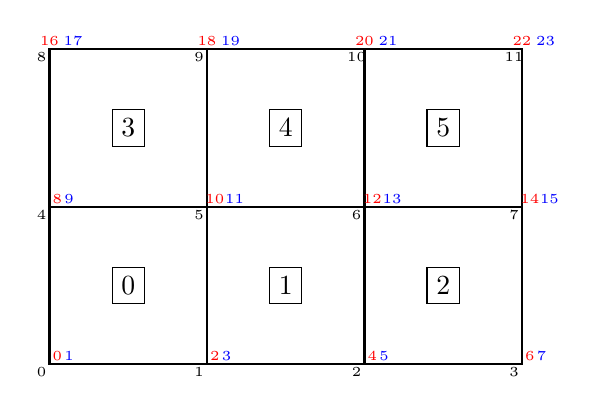
\begin{tikzpicture}
%\draw[step=0.5cm,gray,very thin] (0,0) grid (8,6); %background grid
\draw[thick] (1,1) -- (3,1) -- (3,3) -- (1,3) -- cycle;  
\draw[thick] (3,1) -- (5,1) -- (5,3) -- (3,3) -- cycle; 
\draw[thick] (5,1) -- (7,1) -- (7,3) -- (5,3) -- cycle; 
\draw[thick] (1,3) -- (3,3) -- (3,5) -- (1,5) -- cycle;  
\draw[thick] (3,3) -- (5,3) -- (5,5) -- (3,5) -- cycle; 
\draw[thick] (5,3) -- (7,3) -- (7,5) -- (5,5) -- cycle; 
\node[draw] at (2,2) {0};
\node[draw] at (4,2) {1};
\node[draw] at (6,2) {2};
\node[draw] at (2,4) {3};
\node[draw] at (4,4) {4};
\node[draw] at (6,4) {5};
%pressure dofs
\node at (0.9,0.9) {\tiny 0};
\node at (2.9,0.9) {\tiny 1};
\node at (4.9,0.9) {\tiny 2};
\node at (6.9,0.9) {\tiny 3};
\node at (0.9,2.9) {\tiny 4};
\node at (2.9,2.9) {\tiny 5};
\node at (4.9,2.9) {\tiny 6};
\node at (6.9,2.9) {\tiny 7};
\node at (0.9,4.9) {\tiny 8};
\node at (2.9,4.9) {\tiny 9};
\node at (4.9,4.9) {\tiny 10};
\node at (6.9,4.9) {\tiny 11};
%velocity dofs
\node[red] at (1.1,1.1) {\tiny 0};  \node[blue] at (1.25,1.1) {\tiny 1};
\node[red] at (3.1,1.1) {\tiny 2};  \node[blue] at (3.25,1.1) {\tiny 3};
\node[red] at (5.1,1.1) {\tiny 4};  \node[blue] at (5.25,1.1) {\tiny 5};
\node[red] at (7.1,1.1) {\tiny 6};  \node[blue] at (7.25,1.1) {\tiny 7};
\node[red] at (1.1,3.1) {\tiny 8};  \node[blue] at (1.25,3.1) {\tiny 9};
\node[red] at (3.1,3.1) {\tiny 10}; \node[blue] at (3.35,3.1) {\tiny 11};
\node[red] at (5.1,3.1) {\tiny 12}; \node[blue] at (5.35,3.1) {\tiny 13};
\node[red] at (7.1,3.1) {\tiny 14}; \node[blue] at (7.35,3.1) {\tiny 15};
\node[red] at (1.,5.1) {\tiny 16}; \node[blue] at (1.3,5.1) {\tiny 17};
\node[red] at (3.,5.1) {\tiny 18}; \node[blue] at (3.3,5.1) {\tiny 19};
\node[red] at (5.,5.1) {\tiny 20}; \node[blue] at (5.3,5.1) {\tiny 21};
\node[red] at (7.,5.1) {\tiny 22}; \node[blue] at (7.3,5.1) {\tiny 23};
\end{tikzpicture}\\
{\tiny Red color corresponds to the dofs in the x direction, blue color indicates a dof in the y direction.}
\end{center}

We have nnp=12, nel=6, NfemV=24. Let us assume that free slip boundary conditions are applied. 
The boundary conditions {\tt fix\_bc} array is then:
\begin{center}
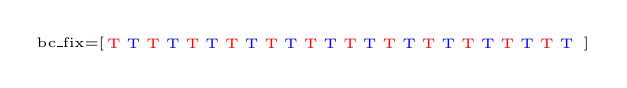
\begin{tikzpicture}
%\draw[step=0.5cm,gray,very thin] (0,0) grid (9,0.7); %background grid
\node  at (0.45,.1) {\tiny bc\_fix=[};

\node[red]  at (1.00,.1) {\tiny T};
\node[blue] at (1.25,.1) {\tiny T};
\node[red]  at (1.50,.1) {\tiny T};
\node[blue] at (1.75,.1) {\tiny T};
\node[red]  at (2.00,.1) {\tiny T};
\node[blue] at (2.25,.1) {\tiny T};
\node[red]  at (2.50,.1) {\tiny T};
\node[blue] at (2.75,.1) {\tiny T};
\node[red]  at (3.00,.1) {\tiny T};
\node[blue] at (3.25,.1) {\tiny T};
\node[red]  at (3.50,.1) {\tiny T};
\node[blue] at (3.75,.1) {\tiny T};
\node[red]  at (4.00,.1) {\tiny T};
\node[blue] at (4.25,.1) {\tiny T};
\node[red]  at (4.50,.1) {\tiny T};
\node[blue] at (4.75,.1) {\tiny T};
\node[red]  at (5.00,.1) {\tiny T};
\node[blue] at (5.25,.1) {\tiny T};
\node[red]  at (5.50,.1) {\tiny T};
\node[blue] at (5.75,.1) {\tiny T};
\node[red]  at (6.00,.1) {\tiny T};
\node[blue] at (6.25,.1) {\tiny T};
\node[red]  at (6.50,.1) {\tiny T};
\node[blue] at (6.75,.1) {\tiny T};

\node  at (7,.1) {\tiny ]};

\end{tikzpicture}\\
\end{center}
Note that since corners belong to two edges, we effectively prescribed 
no-slip boundary conditions on those. 
\todo[inline]{why does array contain only T??}


We wish to compute the tractions on the boundaries, and more precisely for the dofs for which 
a Dirichlet velocity boundary condition has been prescribed.
The number of (traction) unknowns NfemTr is then the number of {\tt T} in the {\tt bc\_fix} array.
In our specific case, we wave NfemTr= .
\todo{finish}
This means that we need for each targeted dof to be able to find its identity/number
between 0 and NfemTr-1. We therefore create the array {\tt bc\_nb} which is 
filled as follows: 
 
\begin{center}
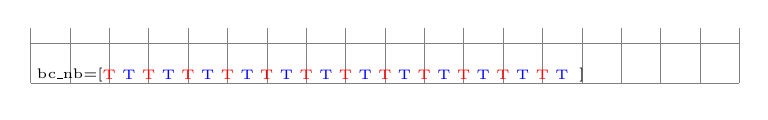
\begin{tikzpicture}
\draw[step=0.5cm,gray,very thin] (0,0) grid (9,0.7); %background grid

\node  at (0.5,.1) {\tiny bc\_nb=[};

\node[red]  at (1.00,.1) {\tiny T};
\node[blue] at (1.25,.1) {\tiny T};
\node[red]  at (1.50,.1) {\tiny T};
\node[blue] at (1.75,.1) {\tiny T};
\node[red]  at (2.00,.1) {\tiny T};
\node[blue] at (2.25,.1) {\tiny T};
\node[red]  at (2.50,.1) {\tiny T};
\node[blue] at (2.75,.1) {\tiny T};
\node[red]  at (3.00,.1) {\tiny T};
\node[blue] at (3.25,.1) {\tiny T};
\node[red]  at (3.50,.1) {\tiny T};
\node[blue] at (3.75,.1) {\tiny T};
\node[red]  at (4.00,.1) {\tiny T};
\node[blue] at (4.25,.1) {\tiny T};
\node[red]  at (4.50,.1) {\tiny T};
\node[blue] at (4.75,.1) {\tiny T};
\node[red]  at (5.00,.1) {\tiny T};
\node[blue] at (5.25,.1) {\tiny T};
\node[red]  at (5.50,.1) {\tiny T};
\node[blue] at (5.75,.1) {\tiny T};
\node[red]  at (6.00,.1) {\tiny T};
\node[blue] at (6.25,.1) {\tiny T};
\node[red]  at (6.50,.1) {\tiny T};
\node[blue] at (6.75,.1) {\tiny T};
\node  at (7,.1) {\tiny ]};
\end{tikzpicture}\\
\end{center}

This translates as follows in the code:
\begin{lstlisting}
NfemTr=np.sum(bc_fix)
bc_nb=np.zeros(NfemV,dtype=np.int32)
counter=0
for i in range(0,NfemV):
    if (bc_fix[i]):
       bc_nb[i]=counter
       counter+=1
\end{lstlisting}


The algorithm is then as follows

\begin{itemize}
\item[A] Prepare two arrays to store the matrix $M_{cbf}$ and its right hand side $rhs_{cbf}$  

\item[B] 
Loop over all elements 

\item[C] 
For each element touching a boundary, compute the residual vector 
$R_{el}=-f_{el} + \K_{el}{\cal V}_{el} + \G_{el} {\cal P}_{el}$

\item[D]
Loop over the four edges of the element using the connectivity array

\item[E]
For each edge loop over the number of degrees of freedom (2 in 2D)

\item[F] 
For each edge assess whether the dofs on both ends are target dofs. 

\item[G]
If so, compute the mass matrix $M_{edge}$ for this edge 

\item[H] extract the 2 values off the element residual vector and assemble these
in $rhs_{cbf}$

\item[I] Assemble $M_{edge}$ into NfemTrxNfemTr matrix using bc\_nb
\end{itemize}


\begin{lstlisting}
M_cbf = np.zeros((NfemTr,NfemTr),np.float64)         # A
rhs_cbf = np.zeros(NfemTr,np.float64)

for iel in range(0,nel):                             # B

    ... compute elemental residual ...               # C

    #boundary 0-1                                    # D
    for i in range(0,ndofV):                         # E
        idof0=2*icon[0,iel]+i
        idof1=2*icon[1,iel]+i
        if (bc_fix[idof0] and bc_fix[idof1]):        # F
           idofTr0=bc_nb[idof0]   
           idofTr1=bc_nb[idof1]
           rhs_cbf[idofTr0]+=res_el[0+i]             # H
           rhs_cbf[idofTr1]+=res_el[2+i]              
           M_cbf[idofTr0,idofTr0]+=M_edge[0,0]       # 
           M_cbf[idofTr0,idofTr1]+=M_edge[0,1]       # I
           M_cbf[idofTr1,idofTr0]+=M_edge[1,0]       # 
           M_cbf[idofTr1,idofTr1]+=M_edge[1,1]       #

    #boundary 1-2                                    #[D]

    ...

    #boundary 2-3                                    #[D]

    ...

    #boundary 3-0                                    #[D]

    ...


\end{lstlisting}










 %--------------------------------------
\newpage %-----------------------------------------------------------------------------------------
\subsection{The value of the timestep} The chosen time step dt used for time integration is chosen to
comply with the Courant-Friedrichs-Lewy condition \cite{cfd_anderson}.
\begin{equation}
\delta t = C \min \left( \frac{h}{\max |{\bm v}|} , \frac{h^2}{\kappa}  \right)
\end{equation}
where $h$ is a measure of the element size, $\kappa = k/ \rho c_p$ 
is the thermal diffusivity and C is the so-called CFL number chosen in $[0,1[$.

In essence the CFL condition arises when solving hyperbolic PDEs \index{hyperbolic PDE}.
It limits the time step in many explicit time-marching computer simulations
so that the simulation does not produce incorrect results. 

This condition is not needed when solving the Stokes equation but it is mandatory 
when solving the heat transport equation or any kind of advection-diffusion equation. 
Note that any increase of grid resolution (i.e. $h$ becomes smaller) yields an automatic 
decrease of the time step value.






 %-----------------------------------------------
\newpage %-----------------------------------------------------------------------------------------
\subsection{Mappings} 
\index{general}{Isoparametric}
The name isoparametric derives from the fact that the same ('iso') 
functions are used as basis functions and for the mapping to the reference element.

More generally, if $n_e$ denotes the number of nodes of an element and $n_g$ denotes the 
number of nodes describing the geometry of the element, 
then the element is termed subparametric when $n_g<n_e$ and 
superparametric when $n_g>n_e$.
\index{general}{Subparametric} \index{general}{Superparametric}

%...........................................
\subsubsection{Linear mapping on a triangle}

\begin{verbatim}
2
|\     s
| \    |_r
|  \
3===1
\end{verbatim}

Let us assume that the coordinates of the vertices are 
$(x_1,y_1)$,  
$(x_2,y_2)$, and 
$(x_3,y_3)$.
The coordinates inside the reference element are $(r,s)$. We then simply have the 
following relationship, i.e. any point of the reference element 
can be mapped to the physical triangle as follows:
\begin{eqnarray}
x&=& r x_1 + s x_2 + (1-r-s) x_3 \\
y&=& r y_1 + s y_2 + (1-r-s) y_3 
\end{eqnarray} 
There is also an inverse map, which is easily computed:
\begin{eqnarray}
r&=& \frac{(y_2-y_3)(x-x_3)-(x_2-x_3)(y-y_3)}{(x_1-x_3)(y_2-y_3)-(y_1-y_3)(x_2-x_3)} \\
s&=& \frac{-(y_1-y_3)(x-x_3)+(x_1-x_3)(y-y_3)}{(x_1-x_3)(y_2-y_3)-(y_1-y_3)(x_2-x_3)} 
\end{eqnarray} 
\begin{remark}
The denominator will not vanish, because it is a multiple of the area of the triangle.
\end{remark}

%................................................
\subsubsection{Bilinear mapping on a linear quadrilateral}

The \index{general}{reference element} is in the $(r,s)$ space. It is a square of size $2\times2$ 
centered around the origin. We wish to map it to the quadrilateral in the $(x,y)$ space:

\begin{center}
\includegraphics[width=8cm]{images/mappings/bilinear/mapping_bilinear.png}
\end{center}

The coordinates of the vertices are 
$(x_1,y_1)$, $(x_2,y_2)$, $(x_3,y_3)$ and $(x_4,y_4)$.
We then simply have the 
following relationship, i.e. any point of the reference element 
can be mapped to the physical quadrilateral as follows:
\begin{eqnarray}
x&=& N_1(r,s) x_1 + N_2(r,s) x_2 + N_3(r,s) x_3 + N_4(r,s) x_4 \\
y&=& N_1(r,s) y_1 + N_2(r,s) y_2 + N_3(r,s) y_3 + N_4(r,s) y_4 
\end{eqnarray} 
where the basis functions $N_i(r,s)$ are defined in section \ref{sec:elts1D}.

In the following example the program randomly generates 10000 points inside the reference 
element and computes their mapping into the $(x,y)$ space. 

\begin{lstlisting}
x1=-1 ; y1=-2
x2=3  ; y2=-1
x3=2  ; y3=2
x4=-3 ; y4=1

npts=10000
r=np.zeros(npts,dtype=np.float64)   
s=np.zeros(npts,dtype=np.float64)   
x=np.zeros(npts,dtype=np.float64)   
y=np.zeros(npts,dtype=np.float64)   

for i in range(0,npts):
    # compute random r,s coordinates
    r[i]=random.uniform(-1.,+1)
    s[i]=random.uniform(-1.,+1)
    # compute basis function values at r,s
    N1=0.25*(1-r[i])*(1-s[i])
    N2=0.25*(1+r[i])*(1-s[i])
    N3=0.25*(1+r[i])*(1+s[i])
    N4=0.25*(1-r[i])*(1+s[i])
    # compute x,y coordinates
    x[i]=N1*x1+N2*x2+N3*x3+N4*x4
    y[i]=N1*y1+N2*y2+N3*y3+N4*y4

np.savetxt('rs.ascii',np.array([r,s]).T)
np.savetxt('xy.ascii',np.array([x,y]).T)
\end{lstlisting}

\begin{center}
\includegraphics[width=7cm]{images/mappings/bilinear/rs.pdf}
\includegraphics[width=7cm]{images/mappings/bilinear/xy.pdf}
\end{center}

There is also an inverse map, which is not so easily computed (see section \ref{sec:amiin}).
However, if the quadrilateral in the $(x,y)$ space is a rectangle of size $(h_x,h_y)$, 
the inverse mapping is trivial:
\begin{eqnarray}
r&=&\frac{x-x_1}{x_2-x_1} \\
s&=&\frac{y-y_1}{y_4-y_1} 
\end{eqnarray}
Also in this case the basis functions can easily be written as functions of $(x,y)$:
\begin{eqnarray}
N_1(x,y) &=& \left( \frac{x_3 -x }{h_x}  \right) \left( \frac{y_3 -y }{h_y}  \right) \nn\\
N_2(x,y) &=& \left( \frac{x - x_1}{h_x}  \right) \left( \frac{y_3 -y }{h_y}  \right) \nn\\
N_3(x,y) &=& \left( \frac{x - x_1}{h_x}  \right) \left( \frac{y - y_1}{h_y}  \right) \nn\\
N_4(x,y) &=& \left( \frac{x_3 -x }{h_x}  \right) \left( \frac{y - y_1}{h_y}  \right) \nn 
\end{eqnarray}

On the one hand, any variable defined on the element can be approximated using the basis functions:
\begin{equation}
f_h(r,s)=\sum_i N_i(r,s) f_i.
\end{equation}
If we treat the coordinate variables $x$ and $y$ themselves as functions, 
then the basis functions can be used to construct the mapping:
\begin{equation}
x(r,s)=\sum_i N_i(r,s) x_i 
\qquad
y(r,s)=\sum_i N_i(r,s) y_i,  \label{eqxy}
\end{equation}
leading to write
\begin{eqnarray}
\frac{\partial x}{\partial r} &=& \sum_i \frac{\partial N_i}{\partial r} x_i \\
\frac{\partial x}{\partial s} &=& \sum_i \frac{\partial N_i}{\partial s} x_i \\
\frac{\partial y}{\partial r} &=& \sum_i \frac{\partial N_i}{\partial r} y_i \\
\frac{\partial y}{\partial s} &=& \sum_i \frac{\partial N_i}{\partial s} y_i 
\end{eqnarray}
On the other hand we also have 
\begin{eqnarray}
\frac{\partial f}{\partial r} &=&
\frac{\partial f}{\partial x}\frac{\partial x}{\partial r}
+\frac{\partial f}{\partial y}\frac{\partial y}{\partial r} \\
\frac{\partial f}{\partial s} &=&
\frac{\partial f}{\partial x}\frac{\partial x}{\partial s}
+\frac{\partial f}{\partial y}\frac{\partial y}{\partial s}
\end{eqnarray}
or in matrix form:
\begin{equation}
\left(
\begin{array}{c}
\frac{\partial f}{\partial r} \\ \\
\frac{\partial f}{\partial s}
\end{array}
\right)
=
\underbrace{
\left(
\begin{array}{cc}
\frac{\partial x}{\partial r} & \frac{\partial y}{\partial r} \nonumber\\ \\
\frac{\partial x}{\partial s} & \frac{\partial y}{\partial s} \nonumber
\end{array}
\right)
}_{\bm J}
\cdot
\left(
\begin{array}{c}
\frac{\partial f}{\partial x} \\ \\
\frac{\partial f}{\partial y}
\end{array}
\right)
\end{equation}
where ${\bm J}$ is called the Jacobian of the transformation
By inverting the Jacobian matrix, the desired derivatives with respect to $x$
and $y$ can be obtained:

We have:
\[
\left(
\begin{array}{c}
\frac{\partial f}{\partial x} \\ \\
\frac{\partial f}{\partial y}
\end{array}
\right)
=
{\bm J}^{-1} \cdot 
\left(
\begin{array}{c}
\frac{\partial f}{\partial r} \\ \\
\frac{\partial f}{\partial s}
\end{array}
\right)
\]
The inverse of the Jacobian matrix can be simply obtained in 
2D (Cramer's rule for $2\times2$ matrices\footnote{\url{https://en.wikipedia.org/wiki/Cramers_rule}}):
\[
{\bm J}^{-1} = \frac{1}{|{\bm J}|} 
\left(
\begin{array}{cc}
\frac{\partial y}{\partial s} & -\frac{\partial y}{\partial r} \nonumber\\ \\
-\frac{\partial x}{\partial s} & \frac{\partial x}{\partial r} \nonumber
\end{array}
\right)
\]
The presence of the determinant in the denominator implies that it cannot 
be zero anywhere, or in other words: the mapping is not valid if $|{\bm J}|$
is zero anywhere over the element.

Note that Hua \cite{hua90} published analytical inverse transformation for quadrilateral
isoparametric elements, i.e. how to compute ${\bm J}^{-1}$ as a function of space coordinates
and not just at the quadrature points. 

Let us look at this by means of a simple example and let us consider the following 
element:
\begin{center}
\includegraphics[width=4cm]{images/mappings/fournode/ex1}
\end{center}
Then a $Q_1$ mapping yields:
\begin{eqnarray}
x(r,s) &=& \sum_i N_i(r,s) x_i = N_2 + 2N_3 = \frac{1}{4} (3+3r+ s+rt) \\
y(r,s) &=& \sum_i N_i(r,s) y_i = 2N_3 + N_4 = \frac{1}{4} (3+r+ 3s+rt) 
\end{eqnarray}
The Jacobian matrix is then
\begin{equation}
{\bm J} = 
\left(
\begin{array}{cc}
\frac{\partial x}{\partial r} & \frac{\partial y}{\partial r} \nonumber\\ \\
\frac{\partial x}{\partial s} & \frac{\partial y}{\partial s} \nonumber
\end{array}
\right)
=
\frac{1}{4}
\left(
\begin{array}{cc}
3+s & 1+s \\
1+r & 3+r
\end{array}
\right)
\end{equation}
and its determinant is 
\begin{equation}
|{\bm J}|=\frac{1}{4} [(3+s)(3+r)-(1+s)(1+r)]=\frac{1}{2}+\frac{1}{8}r+\frac{1}{8}s
\end{equation}
It is clear that $|{\bm J}|>0$ for $-1\leq r \leq +1$ and $-1\leq s \leq +1$. 

Let us now consider another example, the following element:
\begin{center}
\includegraphics[width=4cm]{images/mappings/fournode/ex2}
\end{center}
It follows that
\begin{eqnarray}
x(r,s) &=& \sum_i N_i(r,s) x_i = \frac{1}{4}(1+r)(7+5s) \\ 
y(r,s) &=& \sum_i N_i(r,s) y_i = \frac{1}{4}(17+5r+7s-5rs)
\end{eqnarray}
and the determinant:
\[
|{\bm J}|=\frac{3}{2}-\frac{15r}{4}+\frac{15s}{4}
\]
is zero for $r-s=2/5$. This mapping is invalid!

\begin{remark}
Problems also arise when the Jacobian matrix is nearly singular due to round-off errors.
To avoid problems linked to badly shaped elements, it is recommended that the inside
angles of an element are larger than $15\degree$ and less than $165\degree$.
\end{remark}

From Eq.~\ref{eqxy}, we can also write:
\begin{eqnarray}
dx &=& \frac{\partial x}{\partial r} dr + \frac{\partial x}{\partial s} ds \\
dy &=& \frac{\partial y}{\partial r} dr + \frac{\partial y}{\partial s} ds 
\end{eqnarray},
or, 
\begin{equation}
\left(
\begin{array}{c}
dx \\ dy
\end{array}
\right)
={\bm J}\cdot
\left(
\begin{array}{c}
dr \\ ds
\end{array}
\right)
\end{equation}
This means that 
\begin{equation}
\int \int ... dx dy = \int \int ...|{\bm J}| dr ds
\end{equation}


%.................................................................
\subsubsection{biquadratic mapping of a straight-line face $Q_2$ element }

\begin{center}
\includegraphics[width=8cm]{images/mappings/biquadratic/mapping1}
\end{center}

The reference element now contains 9 nodes: 1,3,7,9 are the corners, nodes
2,4,6,8 are the mid-face points and node 5 is in the middle.
The mapping from the $(r,s)$ space to the $(x,y)$ space is then as follows:

\begin{eqnarray}
\left(
\begin{array}{c}
x(r,s) \\ y(r,s)
\end{array}
\right)
&=&
N_1(r,s)
\left(
\begin{array}{c}
x_1 \\ y_1
\end{array}
\right)
+
N_2(r,s)
\left(
\begin{array}{c}
x_2 \\ y_2
\end{array}
\right)
+
N_3(r,s)
\left(
\begin{array}{c}
x_3 \\ y_3
\end{array}
\right)
+
N_4(r,s)
\left(
\begin{array}{c}
x_4 \\ y_4
\end{array}
\right) \nonumber\\
&+&
N_5(r,s)
\left(
\begin{array}{c}
x_5 \\ y_5
\end{array}
\right)
+
N_6(r,s)
\left(
\begin{array}{c}
x_6 \\ y_6
\end{array}
\right)
+
N_7(r,s)
\left(
\begin{array}{c}
x_7 \\ y_7
\end{array}
\right)
+
N_8(r,s)
\left(
\begin{array}{c}
x_4 \\ y_8
\end{array}
\right) \nonumber\\
&+&
N_9(r,s)
\left(
\begin{array}{c}
x_9 \\ y_9
\end{array}
\right) 
\nonumber
\end{eqnarray}
where
\begin{eqnarray}
N_1(r,t)&=& 0.5r(r-1)  0.5t(t-1) \nonumber\\
N_2(r,t)&=&      (1-r^2)  0.5t(t-1) \nonumber\\
N_3(r,t)&=& 0.5r(r+1)  0.5t(t-1) \nonumber\\
N_4(r,t)&=& 0.5r(r-1)       (1-t^2) \nonumber\\
N_5(r,t)&=&      (1-r^2)       (1-t^2) \nonumber\\
N_6(r,t)&=& 0.5r(r+1)       (1-t^2) \nonumber\\
N_7(r,t)&=& 0.5r(r-1)  0.5t(t+1) \nonumber\\
N_8(r,t)&=&      (1-r^2)  0.5t(t+1) \nonumber\\
N_9(r,t)&=& 0.5r(r+1)  0.5t(t+1) \nonumber
\end{eqnarray}


\begin{lstlisting}
x1=-1                 ; y1=-2
x3=3                  ; y3=-1
x9=2                  ; y9=2
x7=-3                 ; y7=1
x2=0.5*(x1+x3)        ; y2=0.5*(y1+y3)
x4=0.5*(x1+x7)        ; y4=0.5*(y1+y7)
x6=0.5*(x3+x9)        ; y6=0.5*(y3+y9)
x8=0.5*(x7+x9)        ; y8=0.5*(y7+y9)
x5=0.25*(x1+x3+x7+x9) ; y5=0.25*(y1+y3+y7+y9)

npts=10000
r=np.zeros(npts,dtype=np.float64)   
s=np.zeros(npts,dtype=np.float64)   
xQ1=np.zeros(npts,dtype=np.float64)   
yQ1=np.zeros(npts,dtype=np.float64)   
xQ2=np.zeros(npts,dtype=np.float64)   
yQ2=np.zeros(npts,dtype=np.float64)   

for i in range(0,npts):
    # compute random r,s coordinates
    r[i]=random.uniform(-1.,+1)
    s[i]=random.uniform(-1.,+1)
    # compute Q2 basis function values at r,s
    N1= 0.5*r[i]*(r[i]-1.) * 0.5*s[i]*(s[i]-1.)
    N2=       (1.-r[i]**2) * 0.5*s[i]*(s[i]-1.)
    N3= 0.5*r[i]*(r[i]+1.) * 0.5*s[i]*(s[i]-1.)
    N4= 0.5*r[i]*(r[i]-1.) *       (1.-s[i]**2)
    N5=       (1.-r[i]**2) *       (1.-s[i]**2)
    N6= 0.5*r[i]*(r[i]+1.) *       (1.-s[i]**2)
    N7= 0.5*r[i]*(r[i]-1.) * 0.5*s[i]*(s[i]+1.)
    N8=       (1.-r[i]**2) * 0.5*s[i]*(s[i]+1.)
    N9= 0.5*r[i]*(r[i]+1.) * 0.5*s[i]*(s[i]+1.)
    # compute x,y coordinates
    xQ2[i]=N1*x1+N2*x2+N3*x3+N4*x4+N5*x5+N6*x6+N7*x7+N8*x8+N9*x9
    yQ2[i]=N1*y1+N2*y2+N3*y3+N4*y4+N5*y5+N6*y6+N7*y7+N8*y8+N9*y9
    # compute Q1 basis function values at r,s
    N1=0.25*(1-r[i])*(1-s[i])
    N2=0.25*(1+r[i])*(1-s[i])
    N3=0.25*(1+r[i])*(1+s[i])
    N4=0.25*(1-r[i])*(1+s[i])
    # compute x,y coordinates
    xQ1[i]=N1*x1+N2*x3+N3*x9+N4*x7
    yQ1[i]=N1*y1+N2*y3+N3*y9+N4*y7

np.savetxt('rs.ascii',np.array([r,s]).T)
np.savetxt('xyQ1.ascii',np.array([xQ1,yQ1]).T)
np.savetxt('xyQ2.ascii',np.array([xQ2,yQ2]).T)
\end{lstlisting}

\begin{center}
a)\includegraphics[width=4.5cm]{images/mappings/biquadratic/rs.pdf}
b)\includegraphics[width=4.5cm]{images/mappings/biquadratic/xyQ1.pdf}
c)\includegraphics[width=4.5cm]{images/mappings/biquadratic/xyQ2.pdf}\\
{\captionfont a) 10,000 random points in the reference element; b,c) image of these points
by means of a bilinear and biquadratic mapping respectively. When the sides of the element
are straight we see that a $Q_1$ mapping is sufficient.}
\end{center}

%.................................................................
\subsubsection{biquadratic mapping of a not-so straight-line face $Q_2$ element }

We now carry out the same exercise as before but nodes 2 and 8 are no more 
in the middle of nodes 1-3 and 7-9 respectively.

\begin{center}
a)\includegraphics[width=4.5cm]{images/mappings/biquadratic2/rs.pdf}
b)\includegraphics[width=4.5cm]{images/mappings/biquadratic2/xyQ1.pdf}
c)\includegraphics[width=4.5cm]{images/mappings/biquadratic2/xyQ2.pdf}\\
{\captionfont a) 10,000 random points in the reference element; b,c) image of these points
by means of a bilinear and biquadratic mapping respectively. In this case we see that 
the $Q_2$ mapping manages to capture the 'real' shape of the element.}
\end{center}

%.......................................................................
\subsubsection{bilinear, biquadratic and bicubic mapping in an annulus }

In the light of what precedes, we can now ask ourselves how this translates to 
a real geodynamic cas. Let us then consider the case of an annular domain, 
a cross section of a hollow sphere. 
When using quadrilateral elements, the mesh will look similar to this:

\begin{center}
\includegraphics[width=6cm]{images/mappings/curved/annulus_mesh}
\end{center}

We here focus on $Q_1$, $Q_2$ and $Q_3$ mappings. We single out an element, 
and arbitrarily define it as follows in polar coordinates:
\begin{lstlisting}
theta1=23./180.*np.pi
theta2=52./180.*np.pi
R1=1.
R2=1.5
\end{lstlisting}
The $Q_1$ mapping requires four points, the $Q_2$ nine points and the $Q_3$
sixteen points. These are placed equidistantly in the $r,\theta$ coordinate
system, as shown hereunder:

\begin{center}
\includegraphics[width=5cm]{images/mappings/curved/nodesQ1.pdf}
\includegraphics[width=5cm]{images/mappings/curved/nodesQ2.pdf}
\includegraphics[width=5cm]{images/mappings/curved/nodesQ3.pdf}\\
{\captionfont Left to right: position of the nodes for the $Q_1$, $Q_2$ and $Q_3$ mappings.}
\end{center}

As before, we randomly shoot 10,000 points inside the reference element 
and map these out in the $x,y$ space. Resulting swarms of points are shown 
in the following figures:

\begin{center}
\includegraphics[width=5cm]{images/mappings/curved/xy1_keep.pdf}
\includegraphics[width=5cm]{images/mappings/curved/xy2_keep.pdf}
\includegraphics[width=5cm]{images/mappings/curved/xy3_keep.pdf}\\
{\captionfont Left to right: position of the mapped points for the $Q_1$, $Q_2$ and $Q_3$ mappings.}
\end{center}

The image of a square with a $Q_1$ mapping is obviously a quadrilateral
so that it looks like quite a few points land outside of the domain $R_1\leq r\leq R_2$.
Note that points are well within $23\degree \leq \theta \leq 52\degree$, which can 
simply be explained by the fact that the faces of the element are straight lines.

However, it looks like the biquadratic and bicubic mappings are doing a much better 
job at mapping the region of space $R_1\leq r\leq R_2$. In order to characterise 
this better, we now place 10,000 points on the bottom face of the reference element (i.e. $s=-1$)
and once again compute their coordinates in the the $x,y$ space:

\begin{center}
\includegraphics[width=5cm]{images/mappings/curved/xy1.pdf}
\includegraphics[width=5cm]{images/mappings/curved/xy2.pdf}
\includegraphics[width=5cm]{images/mappings/curved/xy3.pdf}\\
{\captionfont Left to right: position of the mapped points for the $Q_1$, $Q_2$ and $Q_3$ mappings.}
\end{center}

For each point $i$ we now compute ist distance $r_i$ 
to the origin, which, if the 
mapping was perfect, whoudl be exactly equal to $R_1=1$. 
On the following plots are shown the error $r_i-1$ for all 
points, from $r=-1$ to $r=+1$.

\begin{center}
\includegraphics[width=5cm]{images/mappings/curved/innerline_error_Q1mapping.pdf}
\includegraphics[width=5cm]{images/mappings/curved/innerline_error_Q2mapping.pdf}
\includegraphics[width=5cm]{images/mappings/curved/innerline_error_Q3mapping.pdf}\\
{\captionfont Left to right: radius error of the mapped points for the $Q_1$, $Q_2$ and $Q_3$ mappings.}
\end{center}

We see that the amplitude of the error decreases with the order of the mapping used, 
which is why for instance ASPECT uses a $Q_4$ mapping by default.
Actually, in this particular case, the equation which describes the cicrle is not a 
polynomial so that no high-order mapping will ever be able to {\it exactly} 
represent the curved boundary of the element!

Another interesting point to keep in mind is that the location of the quadrature points
in the $x,y$ space is also determined by the mapping used, which can have consequences
on the accuracy of the integration and it will be reflected (for instance) on the 
error convergence rate.

Finally, the coordinates of the nodes of the element in the $x,y$ are 
uniquely determined when they are on the convex hull of the element (
for instance nodes 0-7 for $Q_2$) but we need to choose the position 
of the last nodes which are inside the element. Unfortunately, this choice is 
not neutral. 

\todo[inline]{re ask Wolfgang about this - correlate with deal.ii}

\vspace{1cm}

\Literature \cite{yuhy94}








 
 %-----------------------------------------------------------
\newpage %-----------------------------------------------------------------------------------------
\subsection{Exporting data to vtk format} 
This format seems to be the universally accepted format for 2D and 3D visualisation in 
Computational Geodynamics (and even CFD ?). Such files can be opened with open source 
softwares such as 
Paraview \footnote{https://www.paraview.org/}, 
MayaVi \footnote{https://docs.enthought.com/mayavi/mayavi/}
or Visit \footnote{https://wci.llnl.gov/simulation/computer-codes/visit/}.

Unfortunately it is my experience that no simple tutorial exists about how to build 
such files. There is an official document which describes the vtk 
format\footnote{https://www.vtk.org/wp-content/uploads/2015/04/file-formats.pdf}
but it delivers the information in a convoluted way. I therefore describe hereafter 
how \fieldstone{} builds the vtk files. 

I hereunder show vtk file corresponding to a 3x2 grid made of linear elements.
In this particular example there are:
\begin{itemize}
\item 12 nodes and 6 elements
\item 1 elemental field: the pressure {\tt p})
\item 2 nodal fields: 1 scalar (the smoothed pressure {\tt q}), 1 vector (the velocity field {\tt u,v,0})
\end{itemize}
Note that vtk files are inherently 3D so that even in the case of a 2D simulation the $z$-coordinate 
of the points and for instance their $z$-velocity component must be provided.
The file, usually called {\filenamefont solution.vtk} starts with a header:

\lstinputlisting[language=python,firstline=1,lastline=3]{images/vtk/solution.vtu}

We then proceed to write the node coordinates as follows:

\lstinputlisting[language=python,firstline=4,lastline=19]{images/vtk/solution.vtu}

These are followed by the elemental field(s):

\lstinputlisting[language=python,firstline=20,lastline=29]{images/vtk/solution.vtu}

Nodal quantities are written next:

\lstinputlisting[language=python,firstline=30,lastline=59]{images/vtk/solution.vtu}

To these informations we must append 3 more datasets. The first one is the connectivity, 
the second one is the offsets and the third one is the type. The first one is trivial
since said connectivity is needed for the Finite Elements. The second must be understood as follows:
when reading the connectivity information in a linear manner the offset values 
indicate the beginning of each element (omitting the zero value). The third simply is the type of element 
as given in the vtk format document (9 corresponds to a generic quadrilateral with an 
internal numbering consistent with ours). 

\lstinputlisting[language=python,firstline=60,lastline=85]{images/vtk/solution.vtu}

The file is then closed with

\lstinputlisting[language=python,firstline=86,lastline=88]{images/vtk/solution.vtu}

The {\sl solution.vtu} file can then be opened with ParaView, MayaVi or Visit and the reader 
is advised to find tutorials online on how to install and use these softwares. 

\begin{center}
\includegraphics[width=4cm]{images/vtk/grid}
\includegraphics[width=4cm]{images/vtk/vel}
\includegraphics[width=4cm]{images/vtk/press}
\end{center}

 %-------------------------------
\newpage %-----------------------------------------------------------------------------------------
\subsection{Runge-Kutta methods} These methods were developed around 1900 by the German mathematicians Carl Runge and Martin Kutta.
The RK methods are methods for the numerical integration of 
ODEs\footnote{\url{https://en.wikipedia.org/wiki/Runge-Kutta_methods}}. These methods are well 
documented in any numerical analysis textbook and the reader is referred to \cite{gery10,tack10}.
Any Runge-Kutta method is uniquely identified by its Butcher tableau (REF?) which contains 
all necessary coefficients to build the algorithm.\todo{missing refs for Butcher tableau}

The simplest Runge-Kutta method is the (forward) Euler method. Its tableau is:

\begin{mdframed}[backgroundcolor=blue!5]
\begin{tabular}{c|c}
0 & \\
\hline
 & 1
\end{tabular}
\end{mdframed}

\index{general}{Midpoint Method} \index{general}{RK2}
The standard second-order RK method method (also called midpoint method) is:

\begin{mdframed}[backgroundcolor=blue!5]
\begin{tabular}{c|cccccc}
0 & \\
1/2 & 1/2 \\
\hline
 & 0 & 1 
\end{tabular}
\end{mdframed}

\index{general}{Heun's emthod}
Another second-order RK method, called Heun's 
method\footnote{\url{https://en.wikipedia.org/wiki/Heun's_method}} is follows:

\begin{mdframed}[backgroundcolor=blue!5]
\begin{tabular}{c|cccccc}
0 & \\
1 & 1 \\
\hline
 & 1/2 & 1/2 
\end{tabular}
\end{mdframed}

A third-order RK method is as follows:\index{general}{RK3}

\begin{mdframed}[backgroundcolor=blue!5]
\begin{tabular}{c|ccccc}
0 & \\
1/2 & 1/2 \\
1 & -1 & 2 \\ 
\hline
 & 1/6 & 4/6  & 1/6
\end{tabular}
\end{mdframed}


\index{general}{RK4}
The RK4 method falls in this framework. Its tableau is:

\begin{mdframed}[backgroundcolor=blue!5]
\begin{tabular}{c|cccccc}
0 & \\
1/2 & 1/2 \\
1/2 & 0 & 1/2 \\
1 & 0 & 0 & 1 \\
\hline
 & 1/6 & 1/3 & 1/3 & 1/6 
\end{tabular}
\end{mdframed}

A slight variation of the standard RK4 method is also due to Kutta in 1901 and is called the 3/8-rule. 
Almost all of the error coefficients are smaller than in the standard method but it requires 
slightly more FLOPs per time step. Its Butcher tableau is

\begin{mdframed}[backgroundcolor=blue!5]
\begin{tabular}{c|cccccc}
0 & \\
1/3 & 1/3 \\
2/3 & -1/3 & 1 \\
1 & 1 & -1 & 1 \\
\hline
 & 1/8 & 3/8 & 3/8 & 1/8 
\end{tabular}
\end{mdframed}


\index{general}{RK45} \index{general}{Runge-Kutta-Fehlberg method}
The following method is called the Runge-Kutta-Fehlberg method and is 
commonly abbreviated 
RKF45\footnote{\url{https://en.wikipedia.org/wiki/Runge-Kutta-Fehlberg_method}}. 
Its Butcher tableau is as follows: 

\begin{mdframed}[backgroundcolor=blue!5]
\begin{tabular}{c|cccccc}
0 & \\
1/4 	&1/4\\ 
3/8 	&3/32 		&9/32 \\
12/13 	&1932/2197 	&-7200/2197 &	7296/2197\\
1 	&439/216 	&-8 	&3680/513 &	-845/4104\\
1/2 	&-8/27 		&2 	&-3544/2565& 	1859/4104 &	-11/40 	\\
\hline
&16/135 	&0 		&6656/12825 	&28561/56430 	&-9/50& 	2/55\\
&25/216 	&0 	&1408/2565 	&2197/4104 	&-1/5 	&0 
\end{tabular}
\end{mdframed}


The first row of coefficients at the bottom of the table gives the fifth-order accurate method, and the second row gives the fourth-order accurate method. 

\begin{center}
\includegraphics[width=7cm]{images/rungekutta/fe7}
\includegraphics[width=8.5cm]{images/rungekutta/dp87}\\
{\captionfont Left: 7th order Fehlberg method; Right: 8/7th order Dormand-Prince method.}
\end{center}

\Literature \cite{fehl85,hanw93,dopr80,dopr86,prdo81,caka90,butcher03}


%....................................................................................
\subsubsection{Using RK methods to advect particles/markers \label{sec:rkparticles}}

In the context of geodynamical modelling, one is usually confronted to the following problem:
now that I have a velocity field on my FE mesh, how can I use it to advect the Lagrangian 
markers?

Runge-Kutta methods are used to this effect but only their spatial component is used:
the velocity solution is not recomputed at the intermediate fractional timesteps, i.e. 
only the coefficients of the right hand side of the tableaus is used.

\begin{itemize}
\item The RK1 method is simple.

\begin{tabular}{c|c}
0 & \\
\hline
 & 1
\end{tabular}

\noindent Carry out a loop over markers and 
\begin{enumerate}
\item interpolate velocity $\vec\upnu_{m}$ onto each marker $m$
\item compute new position as follows: $\vec r_m(t+\delta t)=\vec r_m(t) + \vec\upnu_m \delta t$
\end{enumerate}

\item The RK2 method is also simple but requires a bit more work.

\begin{tabular}{c|cccccc}
0 & \\
1 & 1 \\
\hline
 & 1/2 & 1/2 
\end{tabular}

\noindent Carry out a loop over markers and 
\begin{enumerate}
\item interpolate velocity $\vec\upnu_{m}$ onto each marker $m$ at position $\vec r_m$
\item compute new intermediate position as follows: $\vec r_m^{(1)}(t+\delta t)=\vec r_m(t) + \vec\upnu_m \delta t/2$
\item compute velocity $\vec\upnu_{m}^{(1)}$ at position $\vec r_m^{(1)}$
\item compute new position: $\vec r_m(t+\delta t)=\vec r_m(t) + \vec\upnu_m^{(1)} \delta t$ 
\end{enumerate}
Note that the intermediate positions could be in a different element of the mesh so extra 
care must be taken when computing intermediate velocities. 

\item 
The RK3 method introduces two intermediate steps. 

\begin{tabular}{c|ccccc}
0 & \\
1/2 & {\color{chestnut} $\frac{1}{2}$ } \\
1 & {\color{violet}-1} & {\color{violet}2} \\ 
\hline
 & {\color{carrotorange} $\frac16$} & {\color{carrotorange} $\frac46$}  & {\color{carrotorange} $\frac16$}
\end{tabular}

Carry out a loop over markers and 
\begin{enumerate}
\item interpolate velocity $\vec\upnu_{m}$ onto each marker $m$ at position $\vec r_m$
\item compute new intermediate position as follows: 
$\vec r_m^{(1)}(t+\delta t)=\vec r_m(t) + {\color{chestnut} \frac{1}{2}} \vec\upnu_m \delta t$
\item compute velocity $\vec\upnu_{m}^{(1)}$ at position $\vec r_m^{(1)}$
\item compute new intermediate position as follows: 
$\vec r_m^{(2)}(t+\delta t)=\vec r_m(t) + ( {\color{violet}-1} \vec\upnu_m 
+ {\color{violet}2} \vec\upnu_m^{(1)} ) \delta t$
\item compute velocity $\vec\upnu_{m}^{(2)}$ at position $\vec r_m^{(2)}$
\item compute new position: 
$\vec r_m(t+\delta t)=\vec r_m(t) + ( 
{\color{carrotorange} \frac16} \vec\upnu_m + 
{\color{carrotorange} \frac46} \vec\upnu_m^{(1)} + 
{\color{carrotorange} \frac16} \vec\upnu_m^{(2)}    )\delta t$ 
\end{enumerate}

\end{itemize}

The following example is borrowed from \cite{maie12}, itself borrowed from Fullsack \cite[Section 5.4]{full95}.
It is a whirl flow \cite{otti89}, a flow with rotational symmetry in which concentric layers of material
rotate around  a centre with an angular velocity:
\[
\omega(r)= \omega_0 \frac{r}{r_0} \exp\left(-\frac{r}{r_0}  \right)
\]  
The box is $[-0.5,0.5]\times[-0.5,0.5]$, $r_0=0.25$, $\omega_0=0.3$ and $\delta t=1$. 
$60\times 60$ particles are regularly positioned inside the $[-0.3,0.3]\times[-0.3,0.3]$ square.
Maierova \cite{maie12} has carried out this experiment for the above Runge-Kutta methods.

\begin{center}
\includegraphics[height=4cm]{images/rk/maie12a}\\
{\captionfont Model domain with particles colored at three
different time-steps: (A) t = 0 (initial position of particles), (B) t = 50, and (C) t = 200.
The advection is computed using the fourth-order Runge-Kutta scheme. Taken from \cite{maie12}}
\end{center}

\begin{center}
\includegraphics[height=4cm]{images/rk/maie12b}
\includegraphics[height=4cm]{images/rk/maie12c}\\
{\captionfont The same plot as above, but for different advection schemes at t = 100.
Advection was computed using (A) the fourth-order Runge-Kutta scheme, (B) the mid-
point method, (C) Heun's method and (D) the explicit Euler method. Taken from \cite{maie12}}
\end{center}


\bscthesis \index{general}{BSc Thesis}



 %----------------------------------------------
\newpage %-----------------------------------------------------------------------------------------
\subsection{Am I in or not? - finding reduced coordinates}\label{sec:amiin}
It is quite common that at some point one must answer the question:
"Given a mesh and its connectivity on the one hand, and the coordinates of a 
point on the other, how do I accurately and quickly determine in which element 
the point resides?"

One typical occurence of such a problem is linked to the use of the Particle-In-Cell 
technique: particles are advected and move through the mesh, and need to be localised 
at every time step. This question could arise in the context of a benchmark where 
certain quantities need to be measured at specific locations inside the domain. 

%-------------------------------------------
%-------------------------------------------
\subsubsection{Two-dimensional space}

We shall first focus on quadrilaterals. There are many kinds of quadrilaterals as shown 
hereunder: 

\begin{center}
\includegraphics[width=10cm]{images/quadrilaterals} % from https://en.wikipedia.org/wiki/Quadrilateral#/media/File:Quadrilaterals.svg
\end{center}

I wish to arrive at a single algorithm which is applicable to all quadrilaterals and therefore 
choose an irregular quadrilateral. For simplicity, let us consider a $Q_1$ element, with a single
node at each corner. 

\begin{center}
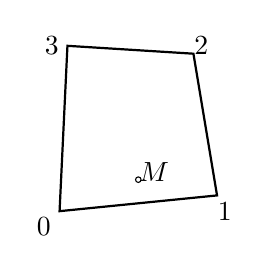
\begin{tikzpicture}
%\draw[step=0.5cm,gray,very thin] (0,0) grid (4,4); %background grid
\draw[thick] (1,1) -- (3,1.2) -- (2.7,3) -- (1.1,3.1) -- cycle;  
\node[] at (0.8,0.8) {0};
\node[] at (3.1,1) {1};
\node[] at (2.8,3.1) {2};
\node[] at (0.9,3.1) {3};
\node[] at (2.2,1.5) {$M$};
\draw (2.,1.4) circle (1pt);
\end{tikzpicture}\\
\end{center}

Several rather simple options exist:
\begin{itemize}
\item we could subdivide the quadrilateral into two triangles and check whether point $M$ is inside any of them (as it turns out, 
this problem is rather straightforward for triangles. Simply google it.)
\item We could check that point $M$ is always on the left side of segments $0\rightarrow 1$, $1\rightarrow 2$, $2\rightarrow 3$, $3\rightarrow 0$.
\item ...  
\end{itemize}

Any of these approaches will work although some might be faster than others. In three-dimensions all will however become 
cumbersome to implement and might not even work at all. Fortunately, there is an elegant way to answer the question, as 
detailed in the following subsection.

%-------------------------------------------
\subsubsection{Three-dimensional space}

If point $M$ is inside the quadrilateral, there exist a set of reduced coordinates $r,s,t\in[-1:1]^3$ such that 

\[
\sum_{i=1}^4 N_i(r_M,s,t) x_i = x_M
\quad\quad\quad
\sum_{i=1}^4 N_i(r_M,s,t) y_i = y_M
\quad\quad\quad
\sum_{i=1}^4 N_i(r_M,s,t) z_i = z_M
\]
This can be cast as a system of three equations and three unknowns. Unfortunately, each shape function $N_i$ 
contains a term $rst$ (as well as $rs$, $rt$, and $st$) so that it is not a linear system and standard techniques
are not applicable. 
We must then use an iterative technique: the algorithm starts with a guess for values $r,s,t$ and 
improves on their value iteration after iteration. 

The classical way of solving nonlinear systems of equations is Newton's method. \index{Newton's method}
We can rewrite the equations above as ${\bm F}(r,s,t)=0$:
\begin{eqnarray}
\sum_{i=1}^8 N_i(r,s,t) x_i - x_M&=&0 \nonumber\\
\sum_{i=1}^8 N_i(r,s,t) y_i - y_M&=&0 \nonumber\\
\sum_{i=1}^8 N_i(r,s,t) z_i - z_M&=&0
\end{eqnarray}
or,
\begin{eqnarray}
F_r(r,s,t)&=&0 \nonumber\\
F_s(r,s,t)&=&0 \nonumber\\
F_t(r,s,t)&=&0 \nonumber
\end{eqnarray}

so that we now have to find the zeroes of continuously differentiable functions ${\bm F}:\mathbb{R} \rightarrow \mathbb{R}$.
The recursion is simply:
\[
\left(
\begin{array}{c}
r_{k+1} \\s_{k+1} \\ t_{k+1}
\end{array}
\right)
=
\left(
\begin{array}{c}
r_{k} \\s_{k} \\ t_{k}
\end{array}
\right)
- J_F(r_k,s_k,t_k) ^{-1} 
\left(
\begin{array}{c}
F_r(r_k,s_k,t_k) \\
F_s(r_k,s_k,t_k)\\
F_t(r_k,s_k,t_k)
\end{array}
\right)
\]
where $J$ the Jacobian matrix:
\begin{eqnarray}
J_F(r_k,s_k,t_k)
&=&
\left(
\begin{array}{ccc}
\frac{\partial F_r}{\partial r}(r_k,s_k,t_k) & \frac{\partial F_r}{\partial s}(r_k,s_k,t_k) & \frac{\partial F_r}{\partial t}(r_k,s_k,t_k) \\\\
\frac{\partial F_s}{\partial r}(r_k,s_k,t_k) & \frac{\partial F_s}{\partial s}(r_k,s_k,t_k) & \frac{\partial F_s}{\partial t}(r_k,s_k,t_k) \\\\
\frac{\partial F_t}{\partial r}(r_k,s_k,t_k) & \frac{\partial F_t}{\partial s}(r_k,s_k,t_k) & \frac{\partial F_t}{\partial t}(r_k,s_k,t_k) 
\end{array}
\right) \nonumber\\
&=&
\left(
\begin{array}{ccc}
\sum\limits_{i=1}^8 \frac{\partial N_i}{\partial r}(r_k,s_k,t_k) x_i &
\sum\limits_{i=1}^8 \frac{\partial N_i}{\partial s}(r_k,s_k,t_k) x_i &
\sum\limits_{i=1}^8 \frac{\partial N_i}{\partial t}(r_k,s_k,t_k) x_i \\
\sum\limits_{i=1}^8 \frac{\partial N_i}{\partial r}(r_k,s_k,t_k) y_i &
\sum\limits_{i=1}^8 \frac{\partial N_i}{\partial s}(r_k,s_k,t_k) y_i &
\sum\limits_{i=1}^8 \frac{\partial N_i}{\partial t}(r_k,s_k,t_k) y_i \\
\sum\limits_{i=1}^8 \frac{\partial N_i}{\partial r}(r_k,s_k,t_k) z_i &
\sum\limits_{i=1}^8 \frac{\partial N_i}{\partial s}(r_k,s_k,t_k) z_i &
\sum\limits_{i=1}^8 \frac{\partial N_i}{\partial t}(r_k,s_k,t_k) z_i 
\end{array}
\right) \nonumber 
\end{eqnarray}
In practice, we solve the following system:
\[
J_F(r_k,s_k,t_k) 
\left[  
\left(
\begin{array}{c}
r_{k+1} \\s_{k+1} \\ t_{k+1}
\end{array}
\right)
-
\left(
\begin{array}{c}
r_{k} \\s_{k} \\ t_{k}
\end{array}
\right)
\right]=-
\left(
\begin{array}{c}
F_r(r_k,s_k,t_k) \\
F_s(r_k,s_k,t_k)\\
F_t(r_k,s_k,t_k)
\end{array}
\right)
\]
Finally, the algorithm goes as follows:
\begin{itemize}
\item set guess values for $r,s,t$ (typically 0)
\item loop over k=0,...
\item Compute rhs= $-{\bm F}(r_k,s_k,t_k)$ 
\item Compute matrix $J_F(r_k,s_k,t_k)$
\item solve system for $(dr_k,ds_k,dt_k)$
\item update $r_{k+1}=r_k+dr_k$, $s_{k+1}=s_k+ds_k$, $t_{k+1}=t_k+dt_k$ 
\item stop iterations when $(dr_k,ds_k,dt_k)$ is small
\item if $r_k,s_k,t_k\in[-1,1]^3$ then $M$ is inside.
\end{itemize}
This method converges quickly but involves iterations, and multiple solves of $3\times 3$ systems which, 
when carried out for each marker and at each time step can prove to be expensive. 
A simple modification can be added to the above algorithm: iterations should be carried out {\it only}
when the point $M$ is inside of a cuboid of size $[\min\limits_i{x_i}:\max\limits_i{x_i}]\times[\min\limits_i{y_i}:\max\limits_i{y_i} ]
\times[\min\limits_i{z_i}:\max\limits_i{z_i}]$ where the sums run over the vertices of the element. 
In 2D this translates as follows: only carry out Newton iterations when $M$ is inside the red rectangle!
\begin{center}
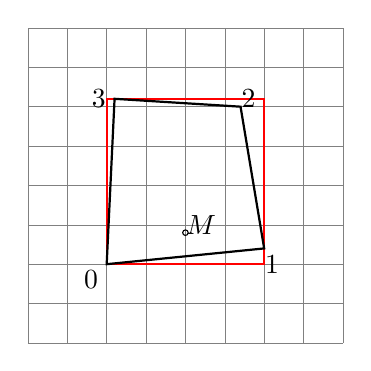
\begin{tikzpicture}
\draw[step=0.5cm,gray,very thin] (0,0) grid (4,4); %background grid
\draw[thick,red] (1,1) -- (3,1) -- (3,3.1) -- (1,3.1) -- cycle;  
\draw[thick] (1,1) -- (3,1.2) -- (2.7,3) -- (1.1,3.1) -- cycle;  
\node[] at (0.8,0.8) {0};
\node[] at (3.1,1) {1};
\node[] at (2.8,3.1) {2};
\node[] at (0.9,3.1) {3};
\node[] at (2.2,1.5) {$M$};
\draw (2.,1.4) circle (1pt);
\end{tikzpicture}\\
\end{center}

Note that the algorithm above extends to high degree elements such as $Q_2$ and higher, even with curved sides.





 %---------
\newpage %-----------------------------------------------------------------------------------------
\subsection{Error measurements and convergence rates} \index{$L_1$ norm}
\index{$L_2$ norm}
\index{$H^1$ norm}

What follows is written in the case of a two-dimensional model. Generalisation to
3D is trivial. What follows is mostly borrowed from \cite{thmk14}.

When measuring the order of accuracy of the primitive variables $\vec{v}$ and $p$,
it is standard to report errors in both the $L_1$ and the $L_2$ norm.
For a scalar quantity $\Psi$, the $L_1$ and $L_2$ norms are computed as
\[
\norm{\Psi}_1 = \int_V |\Psi| dV
\quad\quad
\quad\quad
\norm{\Psi}_2 = \sqrt{ \int_V \Psi^2 dV }
\]
For a vector quantity $\vec{k}=(k_x,k_y)$ in a two-dimensional space,
the $L_1$ and $L_2$ norms are defined as:
\[
\norm{\vec{k}}_1 = \int_V (|k_x|+|k_y|) dV
\quad\quad
\quad\quad
\norm{\vec{k}}_2 = \sqrt{ \int_V (k_x^2+k_y^2) dV }
\]
To compute the respective norms
the integrals in the above norms can be approximated by splitting them
into their element-wise contributions. The element volume integral can then
be easily computed by numerical integration using Gauss-Legendre quadrature.

The respective $L_1$ and $L_2$ norms for the pressure error can be evaluated via
\[
e_p^h|_1 = \sum_{i=1}^{n_e} \sum_{q=1}^{n_q} |e_p^h(\vec{r}_q)| w_q |J_q|
\quad\quad
\quad\quad
e_p^h|_2=\sqrt{ \sum_{i=1}^{n_e} \sum_{q=1}^{n_q} |e_p^h(\vec{r}_q)|^2 w_q |J_q| }
\]
where $e_p^h(\vec{r}_q)=p^h(\vec{r}_q) - p(\vec{r}_q)$ 
is the pressure error evaluated at the $q$-th quadrature associated with
the $i$th element. $n_e$ and $n_q$ refer to the number of elements and
the number of quadrature points per element.
$w_q$ and $J_q$ are the quadrature weight of the Jacobian associated with
point $q$.

The velocity error $e_{\vec v}^h$ is evaluated using the following two norms
\[
e_{\vec{v}}^h|_1 = \sum_{i=1}^{n_e} \sum_{q=1}^{n_q} [ |e_u^h(\vec{r}_q)| + |e_v^h(\vec{r}_q)| ]    w_q |J_q|
\quad\quad
\quad\quad
e_{\vec v}^h|_2=\sqrt{ \sum_{i=1}^{n_e} \sum_{q=1}^{n_q} \left[ |e_u^h({\bm r}_q)|^2 +  e_v^h({\bm r}_q)|^2 \right] w_q |J_q| }
\]
where $e_u^h(\vec{r}_q)=u^h(\vec{r}_q) - u(\vec{r}_q)$ and $e_v^h(\vec{r}_q)=v^h(\vec{r}_q)-v(\vec{r}_q)$.




\index{$H^1(\Omega)$ space} \index{$H^1$ norm} \index{$H^1$ semi-norm}
Another norm is very varely used in the geodynamics literature but is preferred in the 
Finite Element literature: the so-called $H^1$ norm. The mathematical basis for this
norm and the nature of the $H^1(\Omega)$ Hilbert space is to be found in many FE books \cite{dohu03,john16,hugh}.
This norm is expression is expressed as follows for a function $f$ such that $f,|\nabla f|\in L^2(\Omega)$
\footnote{\url{https://en.wikipedia.org/wiki/Sobolev_space}}
\[
\norm{f}_{H^1} = \left( \int_\Omega ( |f|^2 + |\nabla f|^2  ) d\Omega   \right)^{1/2}
\]
We then have 
\[
e_{\vec v}^h|_{H^1} = \norm{\vec{v}^h-\vec{v}}_{H^1} = \sqrt{
\sum\limits_{i=1}^d 
\int_\Omega  
\left[
({v}_i^h-{v}_i)^2
+
\vec\nabla(v_i^h-v_i)\cdot\vec\nabla(v_i^h-v_i) 
\right] d\Omega   
}
\]
where $d$ is the number of dimensions.
Note that sometimes the following semi-norm is used \cite{dobo04,bodg06}:
\[
e_{\vec v}^h|_{H^1} = \norm{\vec{v}^h-\vec{v}}_{H^1} = \sqrt{
\sum\limits_{i=1}^d 
\int_\Omega  
\left[
\vec\nabla(v_i^h-v_i)\cdot\vec\nabla(v_i^h-v_i) 
\right] d\Omega   
}
\]
 

When computing the different error norms for $e_p$ and $e_{\vec v}$ for a set of numerical experiments with
varying resolution $h$ we expect the error norms to follow the following relationships:
\[
e_{\vec v}^h|_1 = C h^{rvL_1} 
\quad\quad\quad\quad
e_{\vec v}^h|_2 = C h^{rvL_2} 
\quad\quad\quad\quad 
e_{\vec v}^h|_{H^1} = C h^{rvH^1}
\]
\[
e_p^h|_1 = C h^{rpL_1} 
\quad\quad\quad 
e_p^h|_2 = C h^{rpL_2}
\]
where $C$ is a resolution-independent constant
and $rpXX$ and $rvXX$ are the convergence rates for
pressure and velocity in various norms, respectively. 
Using linear regression on the logarithm of the respective error norm and the resolution $h$,
one can compute the convergence rates of the numerical solutions.

As mentioned in \cite{dobo04}, when finite element solutions converge at
the same rates as the interpolants we say that the method is optimal, i.e.:
\index{optimal rate}

\[
e_{\vec v}^h|_{L_2} = {\cal O}(h^3)
\quad\quad\quad\quad
e_{\vec v}^h|_{H^1} = {\cal O}(h^2)
\quad\quad\quad\quad
e_{p}^h|_{L_2} = {\cal O}(h^2)
\]

%\begin{itemize}
%\item For $Q_1P_0$, the theoretical lower bound for $r_v'$ is 2 and for $r_p'$ it is 1
%\item For $Q_2P_{-1}$, the theoretical lower bound for $r_v'$ is 3 and for $r_p'$ it is 2
%\end{itemize}
We note that when using discontinuous pressure space
(e.g., $P_0$, $P_{-1}$), these bounds remain valid even
when the viscosity is discontinuous provided that the element boundaries conform to the discontinuity.

 
\subsubsection{About extrapolation}
\index{Extrapolation}

{\it Section contributed by W. Bangerth and part of Thieulot \& Bangerth [in prep.]}

In a number of numerical benchmarks we
want to estimate the error $X_h-X^\ast$ between a quantity $X_h$ computed
from the numerical solution $\vec{u}_h,p_h$ and the corresponding value
$X$ computed from the exact solution $\vec{u},p$. Examples of such quantities
$X$ are the root mean square velocity $v_{rms}$, but it could also be a mass flux
across a boundary, an average horizontal velocity at the top boundary, or
any other scalar quantity.

If the exact solution is known, then one can of course compute $X$ from it.
On the other hand, we would of course like to assess convergence also in
cases where the exact solution is not known. In that case, one can compute
an \textit{estimate} $X^\ast$ for $X$ by way of \textit{extrapolation}.
To this end, we make the assumption that asymptotically, $X_h$ converges to
$X$ at a fixed (but unknown) rate $r$, so that
\begin{equation}
  \label{eq:extrapolation-1}
  e_h=|X_h-X| \approx C h^r.
\end{equation}
Here, $X$, $C$ and $r$ are all unknown constants to be determined, although
we are not really interested in $C$.
We can evaluate $X_h$ from the numerical solution
on successively refined meshes with mesh sizes $h$, $h/2$, and $h/4$. Then,
in addition to \eqref{eq:extrapolation-1} we also have
\begin{eqnarray}
  \label{eq:extrapolation-2}
  e_{h/2}=|X_{h/2}-X| \approx C \left(\frac h2\right)^r,
  \\
  \label{eq:extrapolation-3}
  e_{h/4} =|X_{h/4}-X| \approx C \left(\frac h4\right)^r.
\end{eqnarray}
Taking ratios of equations \eqref{eq:extrapolation-1}--\eqref{eq:extrapolation-3},
and replacing the unknown $X$ by an \textit{estimate} $X^\ast$, we then
arrive at the following equation:
\begin{equation*}
\frac{|X_h-X^\star|}{|X_{h/2}-X^\star|}
=
\frac{|X_{h/2}-X^\star|}{|X_{h/4}-X^\star|}=2^r.
\end{equation*}
If one assumes that $X_h$ converges to $X$ uniformly either from above or
below (rather than oscillate around $X$), then this equation allows us
to solve for $X^\ast$ and $r$:
\begin{equation*}
X^\star = \frac{X_h X_{h/2}-X_{h/2}^2}{X_h - 2 X_{h/2} + X_{h/4}}, \qquad\qquad
r = \log_2 \frac{X_{h/2}-X^\star}{X_{h/4}-X^\star}.
\end{equation*}
In the determination of $r$, we could also have used $X_h$ and $X_{h/2}$,
but using $X_{h/2}$ and $X_{h/4}$ is generally more reliable because
the higher order terms we have omitted in \eqref{eq:extrapolation-1} are less
visible on finer meshes.

 %-----------------------------
\newpage %-----------------------------------------------------------------------------------------
\subsection{The initial temperature field} 
\Literature: Thermal gradients in the continental crust \cite{chap86}

\Literature: Simple analytical approximation to the temperature structure in
subduction zones \cite{enwi04}

\Literature: Thermal Structure of Oceanic Lithosphere \cite{rihc18}

%.............................................................
\subsubsection{Single layer with imposed temperature b.c.}

Let us take a single layer of material characterised by
a heat capacity $C_p$, a heat conductivity $k$
and a heat production term $H$.

\begin{center}
\includegraphics[width=5cm]{images/initial_temperature/tempcond.png}
\end{center}

The Heat transport equation writes
\begin{equation}
\rho C_p \left( \frac{\partial T}{\partial t} + {\vec v} \cdot {\vec \nabla} { T} \right) = 
{\vec \nabla} \cdot (k {\vec \nabla} T) + \rho H
\end{equation}
At steady state and in the absence of a velocity field, assuming
that the material properties to be independent of time and space, and 
assuming that
there is no heat production ($H=0$), this equation
simplifies to
\begin{equation}
\Delta T =0 
\end{equation}
Assuming the layer to be parallel to the $x$-axis, the temperature is
$T(x,y)=T(y)=\alpha T+ \beta$. 
In order to specify the constants $\alpha$ and $\beta$, we need two constraints.

At the bottom of the layer $y=y_b$ a temperature $T_b$ is prescribed while a temperature
$T_t$ is prescribed at the top with $y=y_t$. This ultimately yields a temperature field in
the layer given by
\begin{mdframed}[backgroundcolor=blue!5]
\[
T(y) = \frac{T_t-T_b}{y_t-y_b}(y-y_b) + T_b
\]
\end{mdframed}

If now the heat production coefficient is not zero, the differential equation
reads
\begin{equation}
 k \Delta T + H = 0 
\end{equation}
The temperature field is then expected to be of the form
\begin{equation}
T(y)= - \frac{H}{2k} y^2 + \alpha y + \beta 
\end{equation}
Supplied again with the same boundary conditions, this leads to
\[
\beta=T_b + \frac{H}{2k} y_b^2 - \alpha y_b
\]
ie,
\[
T(y) = -\frac{H}{2k} (y^2-y_b^2) + \alpha (y-y_b) + T_b
\]
and finally
\[
\alpha =  \frac{T_t-T_b}{y_t-y_b}  + \frac{H}{2k}(y_b+y_t)
\]
or,
\[
T(y) = -\frac{H}{2k} (y^2-y_b^2) + \left( \frac{T_t-T_b}{y_t-y_b}  + \frac{H}{2k}(y_b+y_t)   \right) (y-y_b) + T_b
\]

Taking $H=0$ in this equation obviously yields the temperature field obtained previously.
Taking $k=2.25$, $T_t=0C$, $T_b=550C$, $y_t=660km$, $y_b=630km$ yields the following
temperature profiles and heat fluxes when the heat production $H$ varies:
\begin{center}
\includegraphics[width=5cm]{images/initial_temperature/temperature1.pdf}
\includegraphics[width=5cm]{images/initial_temperature/heatflux1.pdf}
\end{center}
Looking at the values at the top, which are somewhat estimated to be
about $55-65mW/m^2$ \cite[table 8.6]{jama}, one sees that value $H=0.8e-6$ yields a very acceptable
heat flux.
Looking at the bottom, the heat flux is then about $0.03W/m^2$
which is somewhat problematic since the heat flux at the Moho
is reported to be somewhere between 10 and 20 $mW/m^2$ in \cite[table 7.1]{jama}.


%-----------------------------------------------------
\subsubsection{Single layer with imposed heat flux b.c.}

Let us now assume that heat fluxes are imposed at the top and bottom of the layer:
\begin{center} 
\includegraphics[width=5cm]{images/initial_temperature/tempcond2.png}
\end{center}

We start again from the ODE
\[
k \Delta T + H = 0 
\]
but only integrate it once:
\[
k \frac{dT}{dy}  + H y + \alpha  = 0 
\]
At the bottom $q=k(dT/dy)|_{y=y_b} = q_b$ and at the top
$q=k(dT/dy)|_{y=y_t} = q_t$ so that 

\todo[inline]{to finish}


 
%-----------------------------------------------------
\subsubsection{Single layer with imposed heat flux and temperature b.c. }

\begin{center}
\includegraphics[width=5cm]{images/initial_temperature/tempcond3.png}
\end{center}

\todo[inline]{to finish}


%---------------------------------------------------------------
\subsubsection{Half cooling space}

TODO. 

\Literature \cite{fagm12} 

%---------------------------------------------------------------
\subsubsection{Plate model}

\cite{mcke67}

%.................................
\subsubsection{McKenzie slab}

When doing thermo-mechanical modelling, the initial temperature
field in the domain is of prime importance. This is 
especially true for the temperature in the slab for subduction 
modelling as its rheological behaviour is strongly temperature-dependent. 
One could easily design a simple geometrical initial field but it is 
unlikely to be close to the field of a slowly subducting slab at an angle 
in a hot mantle. 

McKenzie \cite{mcke69} derived such approximate initial field from the 
steady-state energy equation in two dimensions:
\begin{equation}
\rho C_p \vec v \cdot \vec\nabla T = k \vec\nabla^2 T
\end{equation}
We denote by $T_l$ the temperature at the base of the lithosphere
and $l$ its thickness (i.e. the thickness of the slab).

Assuming $\vec v=(v_x,0)$ yields
\[
\rho C_p v_x \frac{\partial T}{\partial x} = k \frac{\partial^2 T}{\partial x^2}
\]
and substitution of $T'=T/T_l$, $x'=x/l$ and $z'=z/l\in[0,1]$ in this equation leads to
\[
\rho C_p v_x \frac{T_l}{l}\frac{\partial T'}{\partial x'} = k \frac{T_l}{l^2}
\left( \frac{\partial^2 T'}{\partial x'^2}
+ \frac{\partial^2 T'}{\partial z'^2} \right)
\]
or 
\[
\frac{\rho C_p v_x l }{k}\frac{\partial T'}{\partial x'} = 
\frac{\partial^2 T'}{\partial x'^2}
+ \frac{\partial^2 T'}{\partial z'^2} 
\]
and finally (see Eq. 2.3 of \cite{mcke69}): 
\[
\frac{\partial^2 T'}{\partial x'^2}
- 2 R \frac{\partial T'}{\partial x'} 
+ \frac{\partial^2 T'}{\partial z'^2} =0
\]
where $R$ is the thermal Reynolds number
\[
R=\frac{\rho C_p v_x l}{2 k}
\] 
The general solution to this PDE with $T'=1$ on the top, left and right boundary is 
\[
T'(x',z')= 1 + \sum_n C_n \exp \left[ \left( R-(R^2+n^2\pi^2)^{1/2} \right) x' \right] \sin (n \pi z')
\]
We now must make an assumption about the temperature on the left boundary ($x'=0$), 
which is the temperature of the lithosphere. 
For simplicity McKenzie assumes that $T'(x'=0,z')=1-z'$ so that $C_n=2(-1)^n/n\pi$ and finally
\begin{mdframed}[backgroundcolor=blue!5]
\begin{equation}
T'(x',z')= 1 + 2\sum_n \frac{(-1)^n}{n \pi} \exp \left[ \left( R-(R^2+n^2\pi^2)^{1/2} \right) x' \right] \sin (n \pi z')
\end{equation}
\end{mdframed}

Let us build a simple temperature model for a $250\text{km}\times 50\text{km}$ slab, 
with $\rho=3000$, $C_p=1250$, $k=3$. The python code is available in {\tt images/mckenzie/mckenzie1.py}.

\begin{center}
\includegraphics[width=0.32\textwidth]{images/mckenzie/temperature_vel0p5.pdf}
\includegraphics[width=0.32\textwidth]{images/mckenzie/temperature_vel1.pdf}
\includegraphics[width=0.32\textwidth]{images/mckenzie/temperature_vel2.pdf}\\
{\captionfont Left to right: Dimensionless temperature $T'$ in a $250\text{km}\times 50\text{km}$ slab 
for $v_x={0.5,1,2}\text{cm/year}$}
\end{center}

We logically recover the fact that the slower the slab penetrates the mantle the more 
temperature diffusion dominates over temperature advection. For $v=0.5\text{cm/year}$ we see that 
that the slab assumes a constant temperature $T'=1$ at all depthes $0\leq z' \leq 1$ for 
$x'\geq 125\text{km}$. 

Note that this field is a steady-state field, valid for a constant density, heat conductivity and 
heat capacity, zero heat production, that it implies that the velocity is constant and that the 
lithosphere temperature is linear. 

One can also embed the slab in a more realistic context, a subduction zone, involving a 
subducting lithosphere, an over-riding plate and a mantle. The domain is $1000\text{km}\times 250\text{km}$.
The mantle temperature is set to $1300\degree$. The slab dip can be varied and so can the 
velocity. The python code is available in {\tt images/mckenzie/mckenzie2.py}.

\begin{center}
\includegraphics[width=0.32\textwidth]{images/mckenzie/temperature2_vel0p5_phi30.pdf}
\includegraphics[width=0.32\textwidth]{images/mckenzie/temperature2_vel1_phi30.pdf}
\includegraphics[width=0.32\textwidth]{images/mckenzie/temperature2_vel2_phi30.pdf}\\
{\captionfont Left to right: temperature $T$ for $v_x={0.5,1,2}\text{cm/year}$ and $\phi=30\degree$.}
\end{center}

\begin{center}
\includegraphics[width=0.32\textwidth]{images/mckenzie/temperature2_vel1_phi15.pdf}
\includegraphics[width=0.32\textwidth]{images/mckenzie/temperature2_vel1_phi30.pdf}
\includegraphics[width=0.32\textwidth]{images/mckenzie/temperature2_vel1_phi45.pdf}\\
{\captionfont Left to right: temperature $T$ for $v_x=1\text{cm/year}$ and $\phi={15,30,45}\degree$.}
\end{center}




%\newpage

%From \cite{mcke70}, Eq. 26:
%\[
%T(r_0) = \theta_1 \exp \left(  \frac{\alpha g}{C_p} (r_1-r_0) \right)
%\]
%where $\theta_1$ is the potential temperature of any piece of the mantle 
%at the earth's surface.
%If $x$ is measured from a depth equal to the thickness of the lithosphere down the
%dip of the slab and $z$ is measured along the normal to the slab from its lower 
%surface, then the dimensionless potential temperature in the slab is 
%\begin{eqnarray}
%\theta'(x',z')
%&=& 1+2\frac{\theta_1-273}{\theta_1} \sum_{n=1}^\infty \frac{(-1)^n}{n \pi}
%\exp \left[ \left( R-(R^2+n^2\pi^2)^{1/2} \right) x' \right] \sin n\pi z' \\
%&=& \frac{1}{\theta_1} \left\{ \theta_1+ 2 (\theta_1-273) \sum_{n=1}^\infty \frac{(-1)^n}{n \pi}
%\exp \left[ \left( R-(R^2+n^2\pi^2)^{1/2} \right) x' \right] \sin n\pi z' \right\}
%\end{eqnarray}
%where $\theta' = \theta/\theta_1$, $x'=x/l$, $z'=z/l$ and 
%with $l$ the thickness of the slab and $v$ its velocity measured down its dip.
%We denote by $\phi$ the dip of the slab so that the depth below the surface $r_1-r_0$ is given by
%$l (x' \sin \phi-z' \cos\phi)$ so that 
%\[
%T(r_0) = \theta_1 \exp \left(  \frac{\alpha g}{C_p} l (x' \sin \phi-z' \cos\phi) \right)
%\]
%The dimensionless scale height $h'$ is defined by $h'=C_p/\alpha g l$ so that
%\[
%T(r_0) = \theta_1 \exp \left[  (x' \sin \phi-z' \cos\phi)/h' \right]
%\]

%Finally,
%\[
%T(x',z')=\exp \left[  (x' \sin \phi-z' \cos\phi)/h' \right] 
%\left\{ \theta_1+ 2 (\theta_1-273) \sum_{n=1}^\infty \frac{(-1)^n}{n \pi}
%\exp \left[ \left( R-(R^2+n^2\pi^2)^{1/2} \right) x' \right] \sin n\pi z' \right\}
%\]

%\todo[inline]{BSc: create mckenzie slab temperature setup}

%......................................................................
\subsubsection{Initial temperature for global mantle convection models}

This is a difficult topic, and Gottschaldt et al \cite{gows09} list a few issues or 
facts to take into account:
\begin{itemize}
\item Frequent  impacts  may  have  determined  the  heat structure of the outer layers (Arrhenius and Lepland 2000), leading to an early thermally stable stratification. 
\item A global magma ocean (Solomatov 2000)  or  several  large  scale  melting events  (Kleine et al. 2004)  are also conceivable. 
\item Fractional crystallisation and subsequent overturn has the potential to result in compositionally or thermally   stable   layering,   too   (Elkins-Tanton et al. 2003; Zaranek and Parmentier 2004)
\end{itemize}


 %---------------------------
\newpage %-----------------------------------------------------------------------------------------
\subsection{Kinematic boundary conditions} \index{general}{Essential Boundary Conditions}
\index{general}{Natural Boundary Conditions}

Boundary conditions come in two basic flavors: essential and natural.
\begin{itemize}
\item Essential bcs directly affect DOFs, and are imposed on the FEM matrix. 
\item Natural bcs do not directly affect DOFs and are imposed on the right-hand side vector.
\end{itemize}

\subsubsection{In-out flux boundary conditions for lithospheric models}

\begin{center}
\includegraphics[width=8cm]{images/boundary_conditions/bc1}\\
\includegraphics[width=8cm]{images/boundary_conditions/drawing.png}
\end{center}

The velocity on the side is given by
\begin{eqnarray}
u(y) &=& v_{ext} \quad\quad y<L_1 \nn\\
u(y) &=& \frac{v_{in}-v_{ext}}{y_2-y_1}(y-y_1) + v_{ext} \quad\quad y_1<y<y_2 \nn\\
u(y) &=& v_{in} \quad\quad y>y_2 \nn
\end{eqnarray}
The requirement for volume conservation is:
\[
\Phi=\int_{0}^{L_y} u(y) dy = 0
\]
Having chosen $v_{in}$ (the velocity of the plate), one can then compute $v_{ext}$
as a function of $y_1$ and $y_2$.

\begin{eqnarray}
\Phi
&=&\int_{0}^{y_1} u(y) dy  +\int_{y_1}^{y_2} u(y) dy +\int_{y_2}^{L_y} u(y) dy \nn\\
&=& v_{ext} y_1  + \frac{1}{2}(v_{in}+v_{ext})(y_2-y_1) + (L_y-y_2) v_{in} \nn\\
&=& v_{ext} [y_1 + \frac{1}{2}(y_2-y_1) ] + v_{in} [ \frac{1}{2}(y_2-y_1)  + (L_y-y_2) ] \nn\\
&=& v_{ext}\frac{1}{2} (y_1 + y_2 ) + v_{in} [ L_y - \frac{1}{2}(y_1+y_2) ] \nn
\end{eqnarray}
and finally
\begin{mdframed}[backgroundcolor=blue!5]
\[
v_{ext} = -v_{in} \frac{ L_y - \frac{1}{2}(y_1+y_2)}{ \frac{1}{2} (y_1 + y_2 ) }
\]
\end{mdframed}

Note that in some cases applying free slip boundary conditions on a curved boundary with a triangular mesh 
can be problematic as explained in Dione \etal (2013) \cite{ditu13}.

\Literature \cite{ensg82}
 %----------------------------------
\newpage %-----------------------------------------------------------------------------------------
\subsection{Computing gradients - the recovery process} 
write about recovering accurate strain rate components and heat flux components on the nodes.

Let $\vec g_f(\vec r)$  be the desired nodal 
field which we want to be the continuous $Q_1$ representation of the field $\vec \nabla f$.
Since the derivative of the shape function does not exist on the nodes we need to design
an algorithm do do so. There are various techniques, as listed hereafter.


%..............................
\subsubsection{Global recovery}




%..................................................
\subsubsection{Local recovery - average over patch}




%........................................................
\subsubsection{Local recovery - least squares over patch}

 %-------------------------
\newpage %-----------------------------------------------------------------------------------------
\subsection{Tracking materials and/or interfaces} 
Unless using a fully Lagrangian formulation, one needs an additional numerical method to represent/track
the various materials present in an undeformable (Eulerian) mesh.
The figure below (by B. Hillebrand) illustrates the three main methods used in geodynamics.

\begin{center}
\includegraphics[width=15cm]{images/tracking/tracking}
\end{center}

Note that what follows is applicable to FEM, FDM, etc ...


A typical test for advection algorithm is the Zalesak disk \cite{zale79}. It is a two dimensional test 
problem of solid body rotation with a constant angular velocity $\omega$ (in rad/sec):

\begin{center}
\includegraphics[width=6cm]{images/tracking/zale79a}
\includegraphics[width=6cm]{images/tracking/zale79b}\\
{\tiny Taken from \cite{zale79}. Left: Schematic representation of two dimensional 
solid body rotation problem. The field inside the cut out has value 3 and it is 1
outside. The rotational speed is such that one full revolution is effected in 
628 cycles. The width of the gap separating the two halves of the cylinder,
as well as the maximum extent of the "bridge" connecting the two halves, is 5 cells.
Right: Perspective view of initial conditions for the two dimensiona! solid body rotation
problem. Note that only a $50\times50$ portion of the mesh centered on the cylinder is displayed.}
\end{center}

This benchmark is widely used in the literature \cite{supu00,vasv05,dilp06,basd08,zhbl14}.
Note that the Zalesak disc is often supplemented with a cone and a Gaussian features:

\begin{center}
\includegraphics[width=6cm]{images/tracking/leve96}\\
{\tiny Taken from \cite{leve96}. Initial data for solid rotation tests}
\end{center}






%..............................................
\subsubsection{The Particle-in-cell technique}
\index{Particle-in-Cell}  \index{Marker-and-Cell} \index{PIC} \index{MAC}

\begin{remark}
The terms 'particle' and 'marker' are commonly (and unfortunately) interchangeably used in the literature in the context of the particle-in-cell technique. However, one should be aware that the marker-and-cell (MAC) technique is something different: it was invented in the early 60's at the Los Alamos Laboratories by Harlow and Welch \cite{hawe65}. For more information on MAC see the review paper by McKee et al \cite{mctf08}.
\end{remark}

The Particle-in-cell method is by far the most widely used in computational geodynamics. 
In its most basic form it is a rather simple method to implement and this probably owes to its success
and early adoption \cite{popo92}  in non-parallel codes such as SOPALE \cite{full95}, 
I2VIS \cite{geyu03} or CITCOM \cite{mczh04} (Appendix~\ref{app:codes}).
It has been implemented in ASPECT \cite{galh18} and the inherent load balancing issues arising from the parallel implementation as well as from the use of Adaptive Mesh Refinement are discussed. It has also been implemented in the MILAMIN code \cite{daks08} to study LLSVPs \cite{musd15}.

The basic methodology goes as follows:
\begin{enumerate}
\item distribute particles in the domain
\item assign a material identity (and/or any other quantity) to each of them
\item project particle quantities of the Eulerian nodes of the mesh
\item solve the Stokes equations for a new velocity field
\item interpolate the velocity onto the particles
\item move the particles with their respective velocities 
\item go back to step 3
\end{enumerate}  

As it turns out each step above needs to be carefully executed and is more difficult than it 
first looks. 

\paragraph{Distributing particles in the domain}. Let us assume we wish to distribute $N_p$ particles
in the domain. How large must $N_p$ be? To simplify, one end member could be 'as many particles as possible that fit in memory' 
while the other end member could be 'one per element/cell on average'. While the former does not necessarily guarantee a 
desired accuracy while being CPU and memory intensive, the latter will certainly lead to zones in the domain void 
of particles which will be problematic since the projection onto the mesh might yield zero values or very inaccurate values.
How many particles (per element/cell) will be enough?
Also, should the particles be randomly distributed in the domain or on some kind of regular grid? 
See fieldstone 13 (Section~\ref{f13}).

\paragraph{Averaging and projection}. This is a very critical step. Unfortunately, there is no community-wide
agreed-upon method. The problem at hand boils down to: at a given location $(\vec r)$ in space I need a 
quantity which is carried by the particles. 
The first step is to find the particle(s) close to this point. If done naively, this is a very costly affair, 
and begs the question what 'close' means. Finding all particles within a radius $R$ of point $\vec r$ can 
be done very efficiently (e.g. with linked lists, Verlet lists, ...) but the choice of $R$ proves to be critical:
if too small, there may not be any particle inside the circle, and if too large there may be many particles 
inside the circle and the averaging over so many particles in space will prove to be over diffusive. 
In practice, the FD or FE mesh is used to provide an indication of $R$. In FDM, the four cells (or quarter cells) around
a node represent the volume of space containing the particles whose properties are to be averaged \cite{dumg11} 
as illustrated in the following figure:

\begin{center}
\includegraphics[width=12cm]{images/dumg11}\\
{\small Taken from \cite{dumg11}. The "4-cell" and "1-cell" schemes for projecting properties defined on the 
markers (denoted by stars) onto
a node (denoted by the solid circle). (A) The 4-cell scheme. The support of the interpolating function $N_i$ associated
with node $i$ is indicated by the shaded region. Only markers within the support of node $i$ contribute to the projection
operation used to define the nodal value at $i$. The shape of the bilinear interpolation function for node $i$ is indicated in
the lower frame. (B) The 1-cell scheme. The thick lines in the lower frame indicate the grid used to discretize the
Stokes equations, while the thin lines indicate the grid onto which marker properties are projected. The 1-cell scheme
utilizes a compact support of size $\Delta x \times  \Delta y$. The support for nodes $r$, $s$, $t$ are indicated by 
the shaded regions. Only
markers within the nodal support contribute to the projection operation for that node.}
\end{center}

Given that the FEM requires to compute integrals over each element, only the particles inside the element will contribute 
to the average values assigned to the quadrature points. However, one could also decide to first average the properties onto the nodes
before using these nodal values to assign values to the quadrature points. In this case the FDM approach applies. 

Finally, in both FDM and FEM bi/trilinear shape functions are used for the interpolation as they can be interpreted as weighing 
functions. Higher order shape functions could also be used but the standard $Q_2$ shape functions (Section~\ref{sec:shpfct2d})
are 2-nd order polynomials which can take negative values (as opposed to the $Q_1$ shape functions which are strictly positive)
and this can pose problems: in some cases, although all values to be averaged are positive, their weighed average can be negative.
Q1 projection PUCKETT

\todo[inline]{it would be nice to have a Q1 and Q2 drawing of a 1D element and show that indeed negative values arise}   

Assuming that we have established a list of particles, all tracking a field $f(\vec r)$ and that each particle has an 
associated weight $N_i$ (function of the location where the average is to be computed or not), 
we must now compute their average value $<f>$. 
The simplest approach which comes to mind is the (weighed) arithmetic mean ($am$):
\[
\langle f\rangle_{am} = \frac{\sum\limits_{i=1}^n N_i f_i}{\sum\limits_{i=1}^n N_i}
\]  
In the case where $f$ is the (mass) density $\rho$, it is indeed what should be used. 
However, turning now to viscosity $\eta$, we know that its value can vary by many orders of magnitude 
over very short distances.
It is then likely that the average runs over values spanning values between $10^{18}\text{Pa s}$ and $10^{25} \text{Pa s}$.
As explained in \cite{scbe08} the arithmetic averaging tends to 'favour' large values: if the sum runs over 
10 particles, 9 carrying the value $10^{25}$ and 1 carrying the value $10^{19}$, the average value (assuming $N_i=1$ for simplicity)
is then
\[
\langle\eta\rangle = \frac{9\cdot 10^{25}+1\cdot 10^{19}}{10} \simeq 0.9\cdot 10^{25}
\]
which is much much closer to $10^{25}$ than to $10^{19}$.
Other averagings are then commonly used, namely the geometric mean ($gm$)  and the harmonic mean ($hm$), defined as follows:
\[
\langle f\rangle_{gm} = \left( \prod_i f_i^{N_i} \right)^{1/\sum\limits_i N_i} 
\qquad
\text{or, }
\qquad
\log_{10} \langle f \rangle_{gm} = \frac{\sum_i N_i \log_{10} f_i }{\sum\limits_i N_i}  
\]
and 
\[
\langle f\rangle_{hm} = \left( \frac{\sum_{i=1}^n N_i \frac{1}{f_i} }{\sum_i N_i}  \right)^{-1}
\qquad
\text{or, }
\qquad
\frac{1}{\langle f\rangle_{hm} } = \frac{\sum_{i=1}^n N_i \frac{1}{f_i} }{\sum_i N_i}  
\]
The geometric mean can be seen as a form of arithmetic mean of $\log_{10}$ values, while the harmonic mean can be seen as 
a form of arithmetic mean of the inverse values.

Looking back at the above example, the geometric mean of the viscosities is given by 
\[
\log \langle \eta\rangle_{gm} = \frac{9\cdot 25+1\cdot 19}{10} = 24.4 
\qquad \text{or,} \qquad 
\langle \eta\rangle_{gm} \simeq 2.5 \cdot 10^{24}
\]
and the harmonic mean:
\[
\langle\eta\rangle_{hm} \simeq \left( \frac{1}{10 \cdot  10^{19}} \right)^{-1} = 10^{20}
\]
We see that the harmonic mean tends to favour the small values. Also we recover the known property:
\begin{equation}
\langle f \rangle_{am}\quad  \geq \quad
\langle f \rangle_{gm}\quad  \geq \quad
\langle f \rangle_{hm} 
\end{equation}



When all $f_i$ are equal to $f_0$ their computed average should also be equal to $f_0$. As a consequence the 
weights $N_i$ should fulfill the condition $\sum\limits_{i=1}^n N_i=1$.
If all weights are equal, then $N_i=1/n$ and the averagings become:

\begin{equation}
\langle f\rangle_{am} = \frac{1}{n} \sum\limits_{i=1}^n f_i
\qquad
\langle f\rangle_{gm} = \prod_i f_i^{1/n} 
\qquad
\langle f\rangle_{hm} = \left( \frac{1}{n}\sum_i^n \frac{1}{\phi_i} \right)^{-1}
\end{equation}

There are many papers which have looked at particle averagings and projections. 
I will for now simply point to the following ones:
\cite{scbe08}
\cite{deka08}
\cite{dumg11}
\cite{modm03}
\cite{poso08}
\cite{thmk14}
\cite{galh18}
\cite{galb19}.

\todo[inline]{write more about particle averaging and projection}


\paragraph{Interpolation of the velocity onto particles}.

Once the particle $i$ has been localised inside a given element (Section~\ref{sec:amiin}) 
and its reduced coordinates $(r,s,t)$ determined, the velocity at this location can 
be computed through the shape functions:
\[
\vec\upnu_i=\sum_{k=1}^m N_i(r,s,t) \vec\upnu_k
\]
This approach is not without problem: while the nodal velocities $\vec\upnu_k$ are such 
that\footnote{for incompressible flows, of course} 
$\vec\nabla\cdot\vec\upnu=0$ (in the weak sense), the computed velocity $\vec\upnu_i$ 
is not necessarily divergence-free! In order to remedy this, a 
Conservative Velocity Interpolation (CVI) has been proposed in \cite{waav15}.


\paragraph{Moving the particles}

This is discussed in the context of the Runge-Kutta Methods, see Section~\ref{sec:rkparticles}.



%..............................................
\subsubsection{The level set function technique}
\index{Level-set Method} \index{Level-set Function} \index{LSM} \index{LSF} \index{ENO}

This method was developed in the 80's by Stanley Osher and James Sethian \cite{}

The Level-set Method (LSM), as it is commonly used in Computational Fluid Dynamics -- and especially 
in Computational Geodynamics -- represents a close curve $\Gamma$ (say, in our case, the 
interface between two fluids or layers) by means of a function $\phi$ (called the level-set function, or LSF).
$\Gamma$ is then the zero level-set of $\phi$:
\begin{equation}
\Gamma = \left\{ (x,y) \; |\; \phi(x,y)=0 \right\}
\end{equation}
The convention is that $\phi>0$ inside the region delimited by $\Gamma$ and $\phi<0$ outside.
The function value indicates on which side of the
interface a point is located (negative or positive) and this is
used to identify materials. 

Furthermore, if the curve $\Gamma$ moves with a velocity $\vec \upnu$, 
then it satisfies the following equation:
\begin{equation}
\frac{\partial \phi}{\partial t} + \vec\upnu \cdot \vec\nabla \phi = 0 
\end{equation}

The level set function is generally chosen to
be a signed distance function, i.e. $|\vec\nabla \phi| = 1$ everywhere 
and its value is also the distance to the interface.

As explained in \cite{hitg14}, the level-set function $\phi$ is advected 
with the velocity $\vec\upnu$ which is obtained by solving the Stokes equations.
This velocity does not guarantee that after an advection step the signed 
distance quality of the LSF is preserved. 
The LSF then needs to be corrected, which is also called reinitialisation. 
Finally, solving the advection equation must be done in an accurate manner both in time and space,
so that so-called ENO (essentially non-oscillatory) schemes are often employed for the 
space derivative \cite{ossh91,saev10}.


The level set method has not often been used in the geodynamics 
community with some notable exceptions 
\cite{bomh06,bomh07,habm07,grbh07,zlfd08,hagr10,sunh10,suhe10,hitg14}
An overview of the method and applications can
be found in \cite{osfe01}.

Several improvements upon the original LSM have been proposed, 
such as for instance the conservative level set of \cite{zhbl14}.
The most notable difference between CLS method originally proposed by Olsson et al. \cite{olkr05,olkz07}
and standard LS method lies in the choice of LS function. Instead of the signed distance function, the
CLS methods employ the Heaviside function $H(\phi)$ 
\[
H(\phi)=
\left\{
\begin{array}{ll}
1 & \phi>0 \\
1/2 & \phi=0 \\
0 & \phi<0
\end{array}
\right.
\]
where $\phi$ is the signed distance function as in the LSM. 
In practice, a hyperbolic tangent function is used:
\[
H(\phi) = \frac{1}{2} (1+\tan (\phi/2\epsilon))
\]
where $\epsilon$ defines the spreading width of $H$. In the case where there are only 
two fluids (i.e. a single level set is sufficient), the material properties such as density and viscosity
are computed as follows:
\[
\rho=\rho_1+(\rho_2-\rho_1)H(\phi)
\]
\[
\eta=\eta_1+(\eta_2-\eta_1)H(\phi)
\]



%..............................................
\subsubsection{The field/composition technique}
\index{compositional Field}

This is the approach taken by the ASPECT developers \cite{krhb12,hedg17}. 
Each material $i$ is represented by a compositional field $c_i$, 
which takes values between 0 and 1.
Each compositional field is then advected with the (prescribed or computed) Stokes velocity:
\[
\frac{\partial c_i}{\partial t} + {\bm v}\cdot {\bm \nabla }c_i = 0
\]

The value at a point (Finite element node or quadrature point) is 1 if it is in the 
domain covered by the material $i$, and 0 otherwise.
In one dimension, each compositional field is a Heavyside function. 
This approach is somewhat similar to the LSM but the field is essentially 
discontinuous across the interface, which makes it very difficult to advect.  
On the plus side, compositional fields need not be reinitialised, as opposed to LSF's.

Accurate numerical advection is a notoriously difficult problem. Unless very specialised 
techniques are used it often yields undershoot ($c_i<0$) and overshoot ($c_i>0$), which 
ultimately yields mass conservation issues. Also, unless special care is taken, 
compositional fields tend to become more and more diffuse over time: the SUPG method (Section~\ref{sec:supg})
and the entropy viscosity method add small amounts of diffusion to dampen the under- and 
overshoots. This means that at a given point two or more compositions may have values, 
which require some form of averaging. If under- and overshoots are present, these averagings
can become very problematic and even yield meaningless quantities (e.g. negative viscosities).

One rather old and popular filtering approach is the so-called Lenardic and Kaula filter \cite{leka93}:

\begin{center}
\includegraphics[width=6cm]{images/compositions/leka93_filter1}\\
\includegraphics[width=6cm]{images/compositions/leka93_filter2}\\
{\small Taken from Lenardic and Kaula \cite{leka93}}
\end{center}

\begin{center}
\includegraphics[width=16cm]{images/compositions/leka93_filter3}\\
{\small From FENICS book}
\end{center}

\Literature: \cite{vyrc13}

\improvement[inline]{write about DG approach}






%..............................................
\subsubsection{The Volume-of-Fluid method}

\cite{hini81}

%..............................................
\subsubsection{The method of characteristics}

\todo[inline]{ask Arie to write something}

\cite{devv00a}

%.............................................
\subsubsection{The Marker Chain method}
\index{Marker Chain} method. 

Literature: \cite{woid78,chri82,chyu84,vaks97}

More recently, it is used to track the free surface position in a FDM code \cite{chmd19}.


%..............................................
\subsubsection{Hybrid methods}

In Braun et al. \cite{brtf08} a level set method is presented which is based on a 3-D set
of triangulated points, which makes it a hybrid between tracers and level set functions:
in the DOUAR code (Appendix~\ref{app:codes}) the interface is then explicitely tracked by means of the tracers while the LSF is computed 
on the FE nodes. Although very promising in theory, this method proved to be difficult to use in practice
since it requires a) a triangulation of the interfaces at $t=0$ which is not trivial if the geometries
are complex (think about a slab in 3D); b) the addition or removal of tracers because of the interface deformation
and the patching of the triangulation; c) the calculation of the distance to the interfaces for each 
FE node based on the triangle normal vectors. 
This probably explains why the Particle-In-Cell method was later implemented in this code (pers. comm.).
Note that another very similar approach is used in \cite{saev10}.



%..............................................
\subsubsection{Boundary fitted mesh}

This method is rather simple to implement and works well for small deformations. It is 
for instance used by Frehner \cite{freh14} (see online supplementary material) in which it is 
stated: "The numerical grid is set up in such a way that the interface
between different material phases (two layers in this case) coincides with element boundaries. Hence, each
element belongs to a unique material phase and no interpolation is necessary."
With such a method, each element is initally attributed a material phase/number and its material
properties do not change. 








 %-------------------------------
\newpage %-----------------------------------------------------------------------------------------
\subsection{Static condensation} \index{general}{Static Condensation}

The idea behind static condensation is quite simple: in some cases, there are dofs 
belonging to an element which only belong to that element. For instance, the so-called MINI 
element ($P_1^+ \times P_1$) showcases a bubble function in the middle (see section \ref{ss:pair}). 
In the following, $\vec{\cal V}^\star$ corresponds to the list of such dofs inside an element.
The discretised Stokes equations on any element looks like:

\begin{equation}
\left(
\begin{array}{ccc}
\K   & L & \G \\
L^T & \K^\star  & H \\
\G^T & H^T & 0
\end{array}
\right)_e
\left(
\begin{array}{c}
\vec{\cal V} \\ \vec{\cal V}^\star \\ \vec{\cal P}
\end{array}
\right)_e
=
\left(
\begin{array}{c}
\vec{f} \\ \vec{f}^\star \\ \vec{h}
\end{array}
\right)_e
\end{equation}
This is only a re-writing of the elemental Stokes matrix where the matrix $\K$ has been 
split in four parts.
Note that the matrix $\K^\star$ is diagonal.\todo{check}

This can also be re-written in non-matrix form:
\begin{eqnarray}
\K \cdot \vec{\cal V} + L \cdot \vec{\cal V}^\star + \G \cdot \vec{\cal P} &=& \vec{f} \\
L^T V + K^\star \cdot  \vec{\cal V}^\star + H \cdot \vec{\cal P} &=& \vec{f}^\star \\
\G^T \cdot \vec{\cal V} + H^T \vec{\cal V}^\star &=& \vec{h}
\end{eqnarray}
The $\vec{\cal V}^\star$ in the second equation can be isolated:
\[
\vec{\cal V}^\star = \K^{-\star} \cdot ( \vec{f}^\star - L^T \cdot \vec{\cal V} - H \cdot \vec{\cal P})
\]
and inserted in the first and third equations:
\begin{eqnarray}
\K \cdot \vec{\cal V} + L \left[ \K^{-\star} ( \vec{f}^\star - L^T \cdot \vec{\cal V} - H \cdot \vec{\cal P} )  \right] + \G \cdot \vec{\cal P} &=& \vec{f} \\
\G^T \cdot \vec{\cal V} + H^T \left[  \K^{-\star} ( \vec{f}^\star - L^T \cdot \vec{\cal V} - H \cdot \vec{\cal P}) \right]  &=& \vec{h}
\end{eqnarray}
or,
\begin{eqnarray}
(\K-L\cdot \K^{-\star} \cdot L^T)\cdot \vec{\cal V} + (G-L\cdot \K^{-\star} \cdot H) \cdot \vec{\cal P} &=& \vec{f}-L\cdot \K^{-\star} \cdot \vec{f}^\star \\
(G^T -H^T\cdot \K^{-\star}\cdot  L^T ) \cdot \vec{\cal V}  - 
(H^T \cdot \K^{-\star} \cdot H )\cdot \vec{\cal P}   &=& \vec{h} -H^T\cdot \K^{-\star}\cdot \vec{f}^\star
\end{eqnarray}
i.e.
\begin{eqnarray}
\underline{\K} \cdot \vec{\cal V} + \underline{\G}\cdot \vec{\cal P} &=& \underline{\vec{f}} \\
\underline{\G}^T \cdot \vec{\cal V} - \underline{\C} \cdot \vec{\cal P} &=& \underline{\vec{h}}
\end{eqnarray}
with
\begin{eqnarray}
\underline{\K}&=& K-L\cdot \K^{-\star} \cdot L^T \\
\underline{\G}&=& G-L\cdot \K^{-\star} \cdot H \\
\underline{\C}&=& H^T \cdot \K^{-\star} \cdot H \\
\underline{\vec{f}}&=& \vec{f}-L\cdot \K^{-\star} \cdot \vec{f}^\star \\
\underline{\vec{h}}&=& \vec{h} -H^T\cdot \K^{-\star}\cdot \vec{f}^\star
\end{eqnarray}
Note that $\underline{\K}$ is symmetric, and so is the Stokes matrix.


For instance, in the case of the MINI element, the dofs corresponding to the bubble 
could be eliminated at the elemental level, which would make the Stokes matrix smaller
(see book by Braess \cite{braess}). 
However, it is then important to note that static condensation introduces a 
pressure-pressure term which was not there in the original formulation.









 %-------------------------------------
\newpage %-----------------------------------------------------------------------------------------
\subsection{Measuring incompressibility \label{ss_incomp}} 
The velocity divergence error integrated over the whole element is given by
\begin{equation}
e_{div}= \int_\Omega (\vec\nabla\cdot \vec v^h - \underbrace{\vec\nabla\cdot \vec v}_{=0}  ) \; d\Omega
= \int_\Omega (\vec\nabla\cdot \vec v^h) \; d\Omega
\end{equation}
where $\Gamma_e$ is the boundary of element $e$ and $\vec{n}$ is the unit 
outward normal of $\Gamma_e$.

Furthermore, one can show that \cite{dobo04}:
\[
e_{div} = \int_{\Gamma_e} \vec{v}^h\cdot\vec{n} \;  d\Gamma
\]
The reason is as follows and is called the divergence 
theorem\footnote{\url{https://en.wikipedia.org/wiki/Divergence_theorem}}:
suppose a volume $V$ subset of $\mathbb{R}^d$ which is compact
and has a piecewise smooth boundary $S$, and if $\vec F$ is
a continuously differentiable vector field then
\[
\int_V ( \vec\nabla\cdot\vec F)\; dV = \int_S (\vec F \cdot \vec n)\; dS
\]
The left side is a volume integral while the right side is a surface integral.
Note that sometimes the notation $d\vec S = \vec n \; dS $ is used so that 
$\vec F \cdot \vec n \; dS = \vec F \cdot d\vec S$.

The average velocity divergence over an element can be defined as 
\[
<\vec \nabla \cdot \vec v>_e 
= \frac{1}{V_e} \int_{\Omega_e}  (\vec\nabla\cdot\vec v) \; d\Omega
= \frac{1}{V_e} \int_{\Gamma_e} \vec{v}\cdot\vec{n} \; d\Gamma
\]
Note that for elements using discontinuous pressures we shall 
recover a zero divergence element per element (local mass conservation)
while for continuous pressure elements the mass conservation 
is guaranteed only globally (i.e. over the whole domain), see section 3.13.2 of \cite{grsa}.

Note that one could instead compute $<|\vec\nabla\cdot \vec v|>_e$. Either volume or 
surface integral can be computed by means of an appropriate Gauss-Legendre quadrature algorithm.

\improvement[inline]{implement and report}


 %------------------------
\newpage %-----------------------------------------------------------------------------------------
\subsection{Periodic boundary conditions\label{ss_periodic}}\index{general}{Periodic Boundary Conditions}

This type of boundary conditions can be handy in some specific cases such 
as infinite domains. The idea is simple: when material leaves the domain 
through a boundary it comes back in through the opposite boundary (which 
of course presupposes a certain topology of the domain). 

For instance, if one wants to model a gas at the molecular level and wishes 
to avoid interactions of the molecules with the walls of the container, 
such boundary conditions can be used, mimicking an infinite domain in all 
directions. 

Let us consider the small mesh depicted hereunder:

\todo[inline]{missing picture}

We wish to implement horizontal boundary conditions so that 
\[
u_5=u_1
\quad\quad
u_{10}=u_6
\quad\quad
u_{15}=u_{11}
\quad\quad
u_{20}=u_{16}
\]
One could of course rewrite these conditions as constraints and extend the Stokes 
matrix but this approach turns out to be not practical at all. 

Instead, the method is rather simple: replace in the connectivity array the dofs on the right side
(nodes 5, 10, 15, 20) by the dofs on the left side. In essence, we wrap the system upon itself 
in the horizontal direction so that elements 4, 8 and 12 'see' and are 'made of' the nodes 1, 6, 11 and 16.
In fact, this is only necessary during the assembly. Everywhere in the loops nodes 5, 10, 15 and 20 appear 
one must replace them by their left pendants 1, 6, 11 and 16. This autmatically generates a matrix 
with lines and columns corresponding to the $u_5$, $u_{10}$, $u_{15}$ and $u_{20}$ being exactly zero. 
The Stokes matrix is the same size, the blocks are the same size and the symmetric character of the matrix 
is respected. However, there remains a problem. There are zeros on the diagonal 
of the above mentioned lines and columns. One must then place there 1 or a more
appropriate value.

Another way of seeing this is as follows: let us assume we have built and assembled
the Stokes matrix, and we want to impose periodic b.c. so that dof $j$ and $i$ are the same. 
The algorithm is composed of four steps:
\begin{enumerate} 
\item add col $j$ to col $i$
\item add row $j$ to row $i$ (including rhs)
\item zero out row $j$, col $j$
\item put average diagonal value on diagonal ($j,j$)
\end{enumerate} 

\begin{remark}
Unfortunately the non-zero pattern of the matrix with periodic b.c. is not the same 
as the matrix without periodic b.c.
\end{remark}


 %---------------------
\newpage %-----------------------------------------------------------------------------------------
\subsection{Removing rotational nullspace\label{ss_nullspace}} 
When free slip boundary conditions are prescribed in an annulus or
hollow sphere geometry there exists a rotational nullspace, or in other words there exists
a tangential velocity field ('pure rotation') which if added or subtracted to the solution 
does not alter the solution. 

As in the pressure normalisation case (see section \ref{ss_pnorm}), the solution is simple:
\begin{enumerate}
\item fix the tangential velocity at {\it one} node on a boundary, and solve the sytem (the nullspace 
has been removed)
\item post-process the solution to have the velocity field fulfill the required conditions, i.e.
either a zero net angular momentum or a zero net angular velocity of the domain. 
\end{enumerate}

\begin{remark}
In \aspect{} this is available under the option 
"Remove nullspace = angular momentum" and "Remove nullspace = net rotation".
The "angular momentum" option removes a rotation such that the net angular momentum is zero.
The "net rotation" option removes the net rotation of the domain.
\end{remark}

In order to remove the angular momentum, we search for a rotation
vector ${\vec \omega}$ such that
\begin{equation}
\int_\Omega \rho[{\vec r} \times ({\vec v}-{\vec \omega} \times {\vec r})] \; d\vec r= \vec 0
\end{equation}
Recognizing that the angular momentum vector ${\vec H}$ is given by
\begin{equation}
{\vec H} = \int_\Omega \rho{\vec r} \times {\vec v}\; d\vec r
\end{equation}
and that the moment of inertia
(also called inertia tensor)\footnote{\url{https://en.wikipedia.org/wiki/Moment\_of\_inertia}}
 for a continuous body 
 $3\times3$ matrix ${\bm I}$ is given by
\begin{equation}
{\bm I}= 
\int_\Omega \rho(\vec r) [\vec r\cdot\vec r \; \bm 1 - \vec r \times \vec r  ] d\vec r 
\end{equation}
so that the above equation writes:
$
{\vec H}={\bm I}\cdot {\vec \omega}
$
and then ${\vec \omega}={\bm I}^{-1} \cdot {\vec H}$.
A rotation about the rotation vector ${\vec \omega}$ is then subtracted from the velocity 
solution \cite[eq. 26]{zhmt08}:
\begin{equation}
\vec v_{new} = \vec v_{old} - \vec \omega \times \vec r 
\end{equation}

\index{angular velocity} \index{angular momentum}

%...............................
\subsubsection{Three dimensions}

The angular momentum vector is given by:
\begin{equation}
\vec H = \int_\Omega \rho(\vec r) \left( 
\begin{array}{c} 
yw-zv \\ zu-xw \\ xv-yu 
\end{array} \right) d\vec r
\end{equation}
while the inertia tensor for a continuous body is given 
by
\begin{eqnarray}
\bm I
&=&\int_\Omega \rho(\vec r) [\vec r\cdot\vec r \; \bm 1 - \vec r \times \vec r  ] d\vec r \\
&=&\int_\Omega \rho(\vec r) 
\left[
\left(
\begin{array}{ccc}
r^2 & 0 & 0 \\
0 & r^2 & 0 \\
0 & 0 & r^2
\end{array}
\right)
- 
\left(
\begin{array}{ccc}
xx & xy & xz \\
yx & yy & yz \\
zx & zy & zz 
\end{array}
\right)
\right] 
d\vec r \\
&=&\int_\Omega \rho(\vec r) 
\left(
\begin{array}{ccc}
y^2+z^2 & -xy & -xz \\
-yx & x^2+z^2 & -yz \\
-zx & -zy & x^2+y^2 
\end{array}
\right)
d\vec r \\
\end{eqnarray}

The angular velocity\footnote{\url{https://en.wikipedia.org/wiki/Angular_velocity }}
 vector is given by $\vec\omega = \frac{\vec r\times \vec v}{r^2}$
so that the volume-averaged angular velocity of the cylindrical shell is:
\[
<\vec {\omega}> = \frac{1}{|\Omega|} \int_\Omega \frac{{\vec r}\times {\vec v}}{r^2} d\vec r
\]
 Note that it can be straightforwardly computed the same way as the angular momentum
(it is in fact the same equation but without the density):

%-----------------------------
\subsubsection{Two dimensions}

In two dimensions, flow is taking place in the $(x,y)$ plane. This means that $\vec r$ and $\vec v$ are coplanar, 
and therefore that $\vec H$ is perpendicular to the plane, i.e. $\vec H \propto \vec e_z$.
We have then
\begin{equation}
\vec H = \int_\Omega \rho(\vec r) \left( 
\begin{array}{c} 
0 \\ 0 \\ xv-yu 
\end{array} \right) d\vec r
\end{equation}
and 
\begin{equation}
\bm I=
\int_\Omega \rho(\vec r) 
\left(
\begin{array}{ccc}
y^2 & -xy & 0 \\
-yx & x^2 & 0 \\
0 & 0 & x^2+y^2 
\end{array}
\right)
d\vec r 
\end{equation}
The volume-averaged angular velocity is then simply:
\begin{equation}
<\omega_z> = \frac{1}{|\Omega|}\int_\Omega \frac{xv-yu}{r^2}d\vec r
\end{equation}

















 %-----------------
\newpage %-----------------------------------------------------------------------------------------
\subsection{Picard and Newton \label{ss_nonlinear}} \index{nonlinear} \index{Picard iterations} \index{relaxation}

\todo[inline]{explain why our eqs are nonlinear}

%--------------------------------
\subsubsection{Picard iterations}

Let us consider the following system of nonlinear algebraic equations:
\[
\mathbb{A}(\vec X) \cdot \vec X = \vec b(\vec X)
\]
Both matrix and right hand side depend on the solution vector $\vec X$.

For many mildly nonlinear problems, a simple successive substitution 
iteration scheme (also called Picard method) will converge to the solution
and it is given by the simple relationship:
\[
\mathbb{A}(\vec X^n) \cdot \vec X^{n+1} = \vec b(\vec X^n)
\]
where $n$ is the iteration number. 
It is easy to implement:
\begin{enumerate}
\item guess $\vec X^0$ or use the solution from previous time step
\item compute $\mathbb{A}$ and $\vec b$ with current solution vector $\vec X^{old}$
\item solve system, obtain $T^{new}$
\item check for convergence (are $\vec X^{old}$ and $\vec X^{new}$ close enough?)
\item $\vec X^{old} \leftarrow \vec X^{new}$
\item go back to 2.
\end{enumerate}

There are various ways to test whether iterations have converged. The simplest
one is to look at $\norm{\vec X^{old}-\vec X^{new} }$ (in the $L_1$, $L_2$ or maximum norm)
and assess whether this term is smaller than a given tolerance $\epsilon$. 
However this approach poses a problem: in geodynamics, if two consecutively obtained 
temperatures do not change by more than a thousandth of a Kelvin (say $\epsilon=10^{-3}$K )
we could consider that iterations have converged but looking now at velocities which 
are of the order of a cm/year (i.e. $\sim 3\cdot 10^{-11}$m/s) we would need a tolerance 
probably less than $10^{-13}$m/s. We see that using absolute values for a convergence 
criterion is a potentially dangerous affair, which is why one uses a relative 
formulation (thereby making $\epsilon$ a dimensionless parameter):
\[
\frac{\norm{\vec X^{old}-\vec X^{new}}}{\norm{\vec X^{new}}} < \epsilon
\]
Another convergence criterion is proposed by Reddy (section 3.7.2) \cite{reddybook2}:
\[
\left(
\frac{ (\vec X^{old}-\vec X^{new})\cdot(\vec X^{old}-\vec X^{new} ) }{ X^{new}\cdot X^{new}  } 
\right)^{1/2} < \epsilon
\]
Yet another convergence criterion is used in \cite{thie11}: the means $<\vec X^{old}>$, $<\vec X^{new}>$
as well as the variances $\sigma^{old}$ and $\sigma^{new}$ are computed, followed by the 
correlation factor $R$:
\[
R= \frac{ <  (\vec X^{old}-<\vec X^{old}>)\cdot( \vec X^{new}-<\vec X^{new}> )>  }{\sqrt{\sigma^{old}\sigma^{new}}}
\]
Since the correlation is normalised, it takes values between 0
(very dissimilar velocity fields) and 1 (very similar fields). The
following convergence criterion is then used: $1-R < \epsilon$.

\todo[inline]{write about nonlinear residual}


Note that in some instances and improvement in convergence rate can be obtained by use of a 
relaxation formula where one first solves
\[
\mathbb{A}(\vec X^n) \cdot \vec X^{\star} = \vec b(\vec X^n)
\]
and then updates $\vec X^n$ as follows:
\[
\vec X^n = \gamma \vec X^n + (1-\gamma) \vec X^\star 
\quad\quad\quad
0 < \gamma \leq 1
\]
When $\gamma=1$ we recover the standard Picard iterations formula above.

%------------------------------------------
\subsection{Defect correction formulation}

Work in progress. 

We start from the system to solve:
\[
{\bm A}(\vec X) \cdot \vec X = \vec b(\vec X)
\]
with the associated residual vector $\vec F$ 
\[
\vec F(\vec X) = {\bm A}(\vec X) \cdot \vec X - \vec b(\vec X)
\]
The Newton-Raphson algorithm consists of two steps:
\begin{enumerate}
\item solve $\bm J_k \cdot \delta \vec X_k = -\vec F(\vec X_k)$, or in the 
case of the incompressible Stokes equation FEM system:
\[
\left(
\begin{array}{cc}
\bm J^{{\cal V}{\cal V}}_k & \bm J^{{\cal V}{\cal P}}_k \\
\bm J^{{\cal P}{\cal V}}_k & 0
\end{array}
\right)
\cdot
\left(
\begin{array}{c}
\delta \vec {\cal V}_k \\ \delta \vec {\cal P}_k
\end{array}
\right)
=
\left(
\begin{array}{c}
- \vec F_k^{\cal V} \\ -\vec F_k^{\cal P}
\end{array}
\right)
\]

\item update $\vec X_{k+1} = \vec X_k + \alpha_k \delta \vec X_k$
\end{enumerate}
The defect correction Picard approach consists of neglecting the derivative terms present 
in the $J$ terms (Eqs. 16,17,18 of \cite{frbt19}) so that 
\[
\bm J^{{\cal V}{\cal V}}_k \simeq \K_k 
\quad\quad
\bm J^{{\cal V}{\cal P}}_k \simeq \G 
\quad\quad
\bm J^{{\cal P}{\cal V}}_k \simeq \G^T
\]
and step 1 of the above iterations become:
\[
\left(
\begin{array}{cc}
\K_k & \G \\ \G^T & 0
\end{array}
\right)
\cdot
\left(
\begin{array}{c}
\delta \vec {\cal V}_k \\ \delta \vec {\cal P}_k
\end{array}
\right)
=
\left(
\begin{array}{c}
- \vec F_k^{\cal V} \\ -\vec F_k^{\cal P}
\end{array}
\right)
\]


\mscthesis: implement a simple Newton solver and apply it to a few nonlinear benchmarks. \index{MSc Thesis} 
 %----------------------------
\newpage %-----------------------------------------------------------------------------------------
\subsection{Parallel or not?} \label{sec:parallel} \index{general}{Domain Decomposition}

%---------------------------
\subsubsection{Rationale}

Let us assume that we want ro run a simulation of the whole Earth mantle
with a constant resolution of $5\text{km}$. The volume of the mantle is
\[
V_{mantle}=\frac{4}{3}\pi (R_{out}^3-R_{in}^3) \simeq  10^{12}  km^3
\]
while the volume of an element is $V_{e} = 125 \text{km}^3$ (this is 
only an average since the tesselation of a hollow sphere with 
hexahedra yields elements which are not all similar \cite{thie18}).
Consequently, the number of cells needed to discretise the mantle
is 
\[
N_{el}=\frac{V_{mantle}}{V_{e}}\simeq 8\times 10^9
\]
We know that the matrix size is approx. 4 times the number of elements in 3D:
\[
N\simeq 25 \times 10^9
\]
Using between 9 and 125 particles per element (a very conservative number),
the total number of particles is then
\[
N_{particles}  \geq 10^{10}
\]
The unescapable conclusion is that high-resolution 3D 
calculations 
 have a very large memory footprint and require extremely long computational times.

The only way to overcome this problem is by resorting to 
using supercomputers with many processors and large memory capacities.

The idea behind parallel programming is to have each processor carry out 
only a subset of the total number of operations required. In order to reduce 
the memory footprint on each processor, only a subset of the computational
mesh is known by each: one speaks then of domain decomposition.

An example of such a large parallel calculation of 3D convection with 
domain decomposition in a spherical shell can be found in \cite{krhb12}:

\begin{center}
a)\includegraphics[width=7cm]{images/parallel/krhb2}
b)\includegraphics[width=7cm]{images/parallel/krhb1} \\
{\captionfont a)Isocontours of the temperature field; b) Partitioning of the domain onto 512 proc. 
The mesh counts 1,424,176 cells. The solution has approximately 54 million unknowns 
(39 million vel., 1.7 million press., and 13 million temp.)
}
\end{center}


\Literature:
\begin{itemize}
\item Three parallel iterative solvers for the Stokes system, discretized by low order 
tetrahedral elements, are compared with respect to their numerical efficiency and their 
scalability running on up to 786,432 parallel threads. Gmeiner \etal (2016) \cite{gmhj16}
\end{itemize}


%----------------------------------------------
\subsubsection{Strong scaling vs weak scaling}

\begin{center}
\includegraphics[width=16cm]{images/parallel/fig}
\end{center}


 %------------------------------
\newpage %-----------------------------------------------------------------------------------------
\subsection{Stream function} \label{sec:streamfunction} \index{general}{Stream Function}

\Literature \cite{giju98}\cite{scja81}\cite{chyu84}\cite{chri84}\cite{hayu94}\cite{olwh97}




The Stream function (commonly denoted by $\Phi$ or $\Psi$) approach is a useful approach in 
fluid dynamics as it 
can provide relatively quick solutions to 2D incompressible flow problems.
Using a stream function
formulation is numerically convenient because velocity information is contained in a single scalar equation
and pressure vanishes from the solution process.
The stream function is a function of coordinates and time of an inviscid liquid.
It allows to determine the components of velocity by differentiating the stream function 
with respect to the space coordinates. 
A family of curves $\Psi = const$ represent {\it streamlines}, i.e. 
the stream function remains constant along a streamline. 
Although also valid in 3D, this approach is mostly used in 2D because of its 
relative simplicity {\color{red} REFERENCES}.

%........................................
\subsubsection{In Cartesian coordinates}

In two dimensions the velocity is obtained as follows:
\begin{equation}
{\vec \upnu} = (u,v) = \left( \frac{\partial \Psi}{\partial y},-\frac{\partial \Psi}{\partial x} \right) 
\end{equation}
Provided the function $\Psi$ is a smooth enough function, 
this automatically insures that the flow is incompressible:
\begin{equation}
{\vec \nabla}\cdot {\vec \upnu} = 
\frac{\partial u}{\partial x} + \frac{\partial v}{\partial y}
=
\frac{\partial^2 \Psi}{\partial xy} - \frac{\partial^2 \Psi}{\partial xy} =0 
\end{equation}
Assuming constant viscosity, the Stokes equation writes:
\begin{equation}
-{\vec \nabla}p + \eta \Delta {\vec \upnu} + \rho {\vec g} = \vec{0}
\end{equation}
Let us introduce the vector ${\vec{W}}$ for convenience such that in each dimension:
\begin{eqnarray}
W_x&=&-\frac{\partial p}{\partial x} 
+ \eta\left( \frac{\partial^2 u}{\partial x^2} + \frac{\partial^2 u}{\partial x^y} \right) \\
W_y&=&-\frac{\partial p}{\partial y} 
+ \eta \left(\frac{\partial^2 v}{\partial x^2} + \frac{\partial^2 v}{\partial x^y} \right) 
\end{eqnarray}
Taking the curl of the vector ${\vec{W}}$ and only considering the component perpendicular to the $xy$-plane:
\begin{equation}
\frac{\partial W_y}{\partial x} - \frac{\partial W_x}{\partial y}  = 
-\frac{\partial \rho g_y}{\partial x} + \frac{\partial \rho g_x}{\partial y}   
\end{equation}
The advantage of this approach is that the pressure terms cancel out (the curl of a gradient is always zero), 
so that:
\begin{equation}
\frac{\partial}{\partial x}\eta\left( \frac{\partial^2 v}{\partial x^2} + \frac{\partial^2 v}{\partial x^y}  \right) 
- \frac{\partial }{\partial y} \eta \left( \frac{\partial^2 u}{\partial x^2} + \frac{\partial^2 u}{\partial x^y} \right) = 
-\frac{\partial \rho g_y}{\partial x} + \frac{\partial \rho g_x}{\partial y}   
\end{equation}
and then replacing $u,v$ by the their stream function derivatives yields (for a constant viscosity):
\begin{equation}
\eta \left(\frac{\partial^4 \Psi}{\partial x^4} + 
\frac{\partial^4 \Psi}{\partial y^4} + 
2\frac{\partial^4 \Psi}{\partial x^2y^2} \right)
=
-\frac{\partial \rho g_y}{\partial x} + \frac{\partial \rho g_x}{\partial y}   
\end{equation}
or, 
\begin{equation}
\eta {\vec \nabla}^4 \Psi 
=
\left(\frac{\partial^2 }{\partial x^2} + \frac{\partial^2 }{\partial y^2} \right) 
\left(\frac{\partial^2 }{\partial x^2} + \frac{\partial^2 }{\partial y^2} \right) \Psi
=
-\frac{\partial \rho g_y}{\partial x} + \frac{\partial \rho g_x}{\partial y}   
\label{eq:sf1}
\end{equation}
Note that $\vec\nabla^2 \vec\nabla^2 = \vec\nabla^4 $ is known as the Biharmonic operator.
\index{general}{Biharmonic Operator} 

These equations are also to be found in the geodynamics literature, 
see Eq. 1.43 \cite[eq. 1.43]{tack10} or \cite[p 70-71]{gery10}.

In the presence of temperature variations and multiple compositions, 
Trim et al (2020) \cite{trlb20}  use the  following nondimensional 
equation:
\[
\left(
\frac{\partial^2 }{\partial x^2} - 
\frac{\partial^2 }{\partial y^2}  
\right)
\left[ \eta
\left(
\frac{\partial^2 \Psi}{\partial x^2} - 
\frac{\partial^2 \Psi}{\partial y^2}  
\right)
\right]
+4
\frac{\partial^2 }{\partial xy} 
\left[
\eta 
\frac{\partial^2 \Psi}{\partial xy} 
\right]
=
Ra_T \frac{\partial T}{\partial x}-
Ra_C \frac{\partial C}{\partial x}
\]
\todo[inline]{check/rederive this formula!}


%........................................
\subsubsection{In Cylindrical coordinates}

TODO

VERIFY THOSE! minus signs ?
\[
\upnu_r=\frac{1}{r}\frac{\partial \Phi}{\partial \theta} 
\]
\[
\upnu_\theta=-\frac{\partial \Phi}{\partial r} 
\]
 %-------------------
\newpage %-----------------------------------------------------------------------------------------
\subsection{Corner flow} \label{sec:cornerflow} The mantle wedge comprised between the downgoing slab and the overriding plate
has been extensively studied since very important geodynamical processes take place
in it or right above it (slab dehydration and water transport, melting, over-riding plate
deformation, vulcanism, ...).

To first approximation one can approach the problem and simplify it greatly by 
assuming that both plates kinematic behaviour are independent of what happens 
in the wedge, that the wedge geometry does not change over time, that the problem 
is essentially 2D, and that the mantle extends very far away from the actual 
wedge (plates are infinite). 

Under such assumptions, it is possible to derive an analytical solution 
for incompressible Stokes flow in the wedge as documented at p. 224 in  Batchelor \cite{batchelor}.

Literature: \cite{tosl78}

\todo[inline]{FIND refs. check new version of Vol7 theortical geophys}

A corner flow setup is shown hereunder:
\begin{center}
\includegraphics[width=8cm]{images/cornerflow/corner}
\end{center}

\index{general}{Stream Function} \index{general}{Biharmonic Operator}
The solution to this problem is arrived at by means of the stream function $\Phi$, defined 
as $u=-\partial \Phi/\partial y$ and $v=\partial \Phi/partial x$, so that we automatically have $\vec\nabla\cdot\vec\upnu=0$.
As shown in Section~\ref{sec:streamfunction}, the stream function $\Phi$ is then the solution to 
the biharmonic equation
\[
\vec\nabla^2 \vec\nabla^2 \Phi = \vec\nabla^4 \Phi = 0
\]

Considering the geometry of the problem has plates of infinite extent with constant relative
velocity, the solution for velocity everywhere is expected to be independent of $r$. This means the
equation is separable and we will use a solution of the form
\[
\Phi(r,\theta)= R(r) f(\theta)
\]
However, given the infinite extent of the domain, the velocity is expected to be 
independent of $r$, so we postulate $R(r)=r$ (look at the relationship between velocity components and 
stream function), or:
\[
\Phi(r,\theta)= r f(\theta)
\]
and we then have to solve
\[
\Delta \left( \frac{1}{r} (f+f'')\right) = \frac{1}{r^3}(f+2f''+f'''')=0.
\]
The solution of this equation for $f$ is:
\begin{eqnarray}
f(\theta) &=&A \sin\theta + B \cos \theta + C \theta \sin \theta + D \theta \cos \theta   \nn\\
f'(\theta)&=&A \cos\theta - B \sin \theta + C (\sin \theta + \theta \cos \theta) + D (\cos \theta - \theta \sin \theta) \nn
\end{eqnarray}
with
\[
\upnu_r=\frac{1}{r}\frac{\partial \Phi}{\partial \theta} = f'(\theta)
\]
\[
\upnu_\theta=-\frac{\partial \Phi}{\partial r} = -f(\theta)
\]
$A$, $B$, $C$ and $D$ are four constants to be determined by means of the boundary conditions which 
are as follows:
\begin{eqnarray}
\upnu_r(\theta=0)            &=&  0 \nonumber\\
\upnu_\theta(\theta=0)       &=&  0 \nonumber\\
\upnu_r(\theta=\theta_0)     &=&  -U_0 \nonumber\\
\upnu_\theta(\theta=\theta_0)&=&  0 \nonumber
\end{eqnarray}
or,
\begin{eqnarray}
f'(0)= A+D &=& 0 \\
f(0) = B &=& 0 \\
f'(\theta_0) &=& -U_0 \\
f(\theta_0) &=& 0 
\end{eqnarray}

From the second equation it is trivial to see that $B=0$, so that:
\[
f(\theta)=A \sin\theta + C \theta \sin \theta + D \theta \cos \theta
\]
\[
f'(\theta)=A \cos\theta + C (\sin \theta + \theta \cos \theta) + D (\cos \theta - \theta \sin \theta)
\]
From the first one we obtain $D=-A$ so that 
\[
f(\theta)=A (\sin\theta - \theta \cos \theta)  + C \theta \sin \theta 
\]
\[
f'(\theta)=A ( \theta \sin \theta)    + C (\sin \theta + \theta \cos \theta) 
\]
The last two boundary conditions yield:
\[
0=A (\sin\theta_0 - \theta_0 \cos \theta_0)  + C \theta_0 \sin \theta_0 
\]
\[
-U_0 = A ( \theta_0 \sin \theta_0)    + C (\sin \theta_0 + \theta_0 \cos \theta_0) 
\]
or, 
\[
A= - U_0 \frac{\theta_0 \sin\theta_0}{\theta_0^2-\sin^2\theta_0}
\quad\quad
C=   U_0 \frac{\sin\theta_0 - \theta_0 \cos \theta_0}{\theta_0^2-\sin^2\theta_0}
\]
Finally:
\[
(A,B,C,D)=
(
-\theta_0 \sin\theta_0,
0,
\sin\theta_0 - \theta_0 \cos \theta_0,
\theta_0 \sin\theta_0
)
\frac{U_0}{\theta_0^2-\sin^2\theta_0}
\]

We have 
\begin{eqnarray}
{\bm e}_r      &=& \cos\theta {\bm e}_x + \sin\theta {\bm e}_y \\
{\bm e}_\theta &=& -\sin\theta {\bm e}_x + \cos\theta {\bm e}_y
\end{eqnarray}
so that the velocity field can be expressed in cartesian coordinates:
\begin{eqnarray}
{\bm \upnu} 
&=& \upnu_r {\bm e}_r + \upnu_\theta {\bm e}_\theta \nn\\
&=& \upnu_r ( \cos\theta {\bm u}_x + \sin\theta {\bm e}_y) + \upnu_\theta (-\sin\theta {\bm u}_x + \cos\theta {\bm e}_y) \nn\\
&=& ( \upnu_r \cos\theta - \upnu_\theta \sin\theta  ) {\bm e}_x + ( \upnu_r \sin\theta + \upnu_\theta\cos\theta  ) {\bm e}_y
\end{eqnarray}








 %-------------------------------

%\subsection{Steady state thermal problems \label{ss_ss}} \input{steadystate} %-

\newpage
%%%%%%%%%%%%%%%%%%%%%%%%%%%%%%%%%%%%%%%%%%%%%%%%%%%%%%%%%%%%%%%%%%%%%%%%%%%%%%%
\section{Gravity and co}








What follows on this page is an unfinished attempt to link spherical harmonics with 
my 2018 paper. 

We start from the Poisson equation for the gravity potential:
\begin{equation}
\Delta U = 4\pi {\cal G} \rho(\vec{r})
\end{equation}
As a consequence, inside a domain where $\rho=0$, the equation becomes $\Delta U=0$.

Let us assume that the spherical coordinates are appropriate for the problem at hand, and that 
the potential can be decomposed as follows:
\[
U(r,\theta,\phi) = U_r(r) U\bot(\theta,\phi)
\]
The full Laplacian operator in spherical coordinates is given 
by\footnote{\url{https://en.wikipedia.org/wiki/Laplace_operator}}:
\[
\Delta U 
= 
\underbrace{\frac{1}{r^2} \frac{\partial }{\partial r}\left(r^2 \frac{\partial U}{\partial r}\right)}_{\Delta_r}
+
\underbrace{
\frac{1}{r^2 \sin\theta} \frac{\partial }{\partial \theta} \left(\sin\theta \frac{\partial U}{\partial \theta} \right) 
+
\frac{1}{r^2 \sin^2\theta} \frac{\partial^2 U }{\partial \phi^2}
}_{\Delta_\bot}
\]
we then have:
\[
(\Delta_r + \Delta_\bot)(U_r U_\bot)=0
\]
i.e., 
\[
U_\bot \Delta_r U_r + U_r \Delta_\bot U_\bot=0
\]
Assuming $U_\bot=\sum_l\sum_m U_{lm}Y_{lm}$, knowing that spherical 
harmonics functions verify
\[
r^2 \Delta_\bot Y_l^m(\theta,\phi) = -l(l+1) Y_l^m (\theta,\phi)
\]
and assuming for now that the problem at hand is 1st degree (l=1), then 
\[
\Delta_\bot Y_l^m(\theta,\phi) = -\frac{2}{r^2} Y_l^m (\theta,\phi)
\]
and then
\[
\Delta_r U_r - U_r \frac{2}{r^2}=0
\]
make a link with my 2018 paper. 






\newpage
In spherical coordinates, the Laplacian is given by
\[
\Delta = 
\frac{1}{r^2} \frac{\partial }{\partial r} \left( r^2 \frac{\partial }{\partial r} \right)
+
\frac{1}{r^2 \sin^2 \theta} \frac{\partial}{\partial \theta} \left( \sin\theta \frac{\partial }{\partial \theta} \right)
+
\frac{1}{r^2 \sin^2 \theta} \frac{\partial^2}{\partial \phi^2}
\]
We wish to solve Laplace's equation $\Delta T(r,\theta,\phi)=0$ using the method 
of separation of variables:
\[
T(r,\theta,\phi) = R(r) \Theta(\theta) \Phi(\phi)
\]
We can insert this decomposition into the Laplace equation and multiply it by $r^2/R\Theta\Phi$ to obtain
\[
\frac{1}{R} \frac{d}{dr} \left( r^2 \frac{dR}{dr} \right) 
+ 
\frac{1}{\Theta} \frac{1}{\sin \theta} \frac{d}{d\theta} \left( \sin \theta \frac{d\Theta}{d\theta} \right)
+
\frac{1}{\Phi} \frac{1}{\sin^2 \theta} \frac{d^2\Phi}{d\phi^2}
=
0
\]
For reasons that will become clear later, the separation constant  is taken to be $-m^2$:
\begin{eqnarray}
\frac{1}{\Phi} \frac{d^2\Phi}{d\phi^2} &=& -m^2  \label{eq:spha2} \\
-\frac{\sin\theta}{\Theta} \frac{d}{d\theta} \left( \sin \theta \frac{d\Theta}{d\theta} \right)
- \frac{\sin^2\theta}{R} \frac{d}{dr} \left( r^2 \frac{dR}{dr} \right) &=& -m^2  \label{eq:spha2}
\end{eqnarray}
The first equation yields
\[
\Phi(\phi) = 
\left\{
\begin{array}{c}
e^{im\phi} \\ e^{-im\phi}
\end{array}
\right.
\qquad\qquad 
\text{for} \; m=0,1,2,3,...
\]
Note that $m$ must be an integer since $\phi$ is a periodic variable and $\Phi(\phi + 2\pi) = \Phi(\phi)$. 
In the case of $m=0$, the general solution is $\Phi(\phi) = a\phi + b$, but we must choose $a=0$ to
be consistent with $\Phi(\phi + 2\pi) = \Phi(\phi)$. Hence in the case of $m = 0$, only one solution is
allowed.

Eq.~\eqref{eq:spha2} can now be recast in the following form:
\begin{equation}
 \frac{1}{R} \frac{d}{dr} \left( r^2 \frac{dR}{dr} \right) 
= 
-\frac{1}{\Theta}\frac{1}{\sin\theta} \frac{d}{d\theta} \left( \sin \theta \frac{d\Theta}{d\theta} \right) 
+\frac{m^2}{\sin^2\theta} \label{eq:spha3}
\end{equation}
where the separation variable at this step is denoted by $l(l + 1)$ for reasons that will shortly
become clear.
The resulting radial equation is 
\[
\frac{1}{R} \frac{d}{dr} \left( r^2 \frac{dR}{dr} \right)  = l(l+1)
\]
or, 
\[
r^2 \frac{d^2R}{dr^2} + 2 r \frac{dR}{dr} - l(l+1)R =0
\]
The solution is of the form $R=r^s$. To determine the exponent $s$, 
we insert this solution back into the above ODE. The end result is
\[
s(s+1)=l(l+1) \qquad \Rightarrow \qquad s=l \; \text{or} \; s=-l-1
\]
or, 
\[
R(r) = 
\left\{
\begin{array}{c}
r^l \\ r^{-(l+1)}
\end{array}
\right.
\]
Eq.~\eqref{eq:spha3} also yields:
\[
\frac{1}{\sin\theta} \frac{d}{d\theta} \left( \sin\theta \frac{d\Theta}{d\theta} \right) 
+
\left[ l(l+1) - \frac{m^2}{\sin^2\theta} \right] \Theta = 0
\]
One can then carry out the following change of variables $x=\cos\theta$ and $y=\Theta(\theta)$ so that 
the above equation reduces to:
\[
(1-x^2) \frac{d^2 y}{d x^2} - 2x \frac{dy}{dx} + 
\left[ l(l+1)-\frac{m^2}{\sin^2\theta} \right] y =0
\]
This equation is the differential equation for associated Legendre 
polynomials\footnote{\url{https://en.wikipedia.org/wiki/Associated_Legendre_polynomials}}.
\index{general}{Associated Legendre polynomials}
We then have
\[
y=P_l^m(x) \qquad \text{for} \; l=0,1,2,3,... \quad \text{and} \; m=-l,-l+1,...0,...l=1,l
\]
and 
\[
P_l^m(x)= \frac{(-1)^m}{2^l \; l!} (1-x^2)^{m/2}
\frac{d^{l+m}}{dx^{l+m}} (x^2-1)^l
\]
with $m \geq 0$ and $l\geq 0$.
The first few polynomials are
\begin{eqnarray}
P_0^0(\cos\theta)    &=& 1 \nn\\ \nn\\ 
P_1^{-1}(\cos\theta) &=& \frac12 \sin\theta \nn\\ 
P_1^{0}(\cos\theta)  &=&  \cos\theta \nn\\ 
P_1^{+1}(\cos\theta) &=& -\sin\theta \nn\\ \nn\\
P_2^{-2}(\cos\theta) &=& \frac18 \sin^2\theta \nn\\
P_2^{-1}(\cos\theta) &=& \frac12\sin\theta\cos\theta \nn\\
P_2^{0}(\cos\theta)  &=& \frac12(3\cos^2\theta -1) \nn\\
P_2^{+1}(\cos\theta) &=& -3 \sin\theta\cos\theta \nn\\
P_2^{+2}(\cos\theta) &=& 3\sin^2\theta \nn
\end{eqnarray}





In our case the differential equation for the associated Legendre polynomials, given above, depends
on $m^2$ and is therefore not sensitive to the sign of $m$.
Consequently, $P_l^m(x)$ and $P_l^{-m}(x)$ must be equivalent solutions and 
hence proportional to each other, and one can show that
\begin{equation}
P_l^{-m}(\cos\theta) = (-1)^m\frac{(l-m)!}{(l+m)} P_l^m(\cos\theta)
\label{eq:spha4}
\end{equation}
Combining all the results obtained above, we have found that the general solution to
Laplace’s equation is of the form
\begin{mdframed}[backgroundcolor=blue!5]
\[
T(r,\theta,\phi) = 
\left\{
\begin{array}{c}
r^l \\ r^{-(l+1)}
\end{array}
\right\}
P_l^m(\cos\theta) 
\left\{
\begin{array}{c}
e^{im\phi} \\ e^{-im\phi}
\end{array}
\right\}
\]
\end{mdframed}
where $l=0,1,2,3,...$ and $m=-l,-l+1,...,l-1,l$.

When solving the Laplace’s equation in spherical coordinates, it is traditional
to introduce the spherical harmonics, $Y_l^m(\theta,\phi)$:
\begin{equation}
Y_l^m(\theta,\phi) = (-1)^m \sqrt{\frac{2l+1}{4\pi} \frac{(l-m)!}{(l+m)!}} P_l^m(\cos\theta) e^{im\phi}
\qquad 
\textrm{for} \; l=0,1,2,3,... \; \textrm{and} \; m=-l,-l+1,...,l-1,l
\label{eq:spha5}
\end{equation}
The phase factor ($-1$) , introduced originally by Condon and Shortley, is convenient for
applications in quantum mechanics. Note that Eq.~\eqref{eq:spha4} implies that
\[
Y_l^{-m} (\theta, \phi) = (-1)^m Y_l^m (\theta,\phi)^* 
\]
where the star means complex conjugation.

The normalization factor in Eq.~\eqref{eq:spha5} has been
chosen such that the spherical harmonics are normalized to one. In particular, these func-
tions are orthonormal and complete. The orthonormality relation is given by:
\[
\int Y_l^m(\theta,\phi) Y_{l'}^{m'}(\theta,\phi) d\Omega = \delta_{ll'} \delta_{mm'}
\]
where $d\Omega = \sin\theta d\theta d\phi$ is the differential solid angle in spherical coordinates.

It is important to note that there are different normalisations for spherical harmonics.
In this document we choose:
\begin{equation}
Y_l^m(\theta,\phi) = \sqrt{\frac{2l+1}{4\pi} \frac{(l-m)!}{(l+m)!}} P_l^m(\cos\theta) e^{im\phi}
\qquad 
\textrm{for} \; l=0,1,2,3,... \; \textrm{and} \; m=-l,-l+1,...,l-1,l
\label{eq:spha6}
\end{equation}
The first few spherical harmonics are shown below in the real representation (i.e. using $\cos m\phi$  instead of $e^{i m \phi}$) \footnote{\url{https://en.wikipedia.org/wiki/Table_of_spherical_harmonics}} \footnote{\url{https://mathworld.wolfram.com/SphericalHarmonic.html}}:
\begin{eqnarray}
Y_0^0(\theta,\phi)    &=& \sqrt{\frac{1}{4\pi}} \nn\\ \nn\\
Y_1^{-1}(\theta,\phi) &=& \sqrt{\frac{3}{8\pi}} \cos\phi\sin\theta\nn\\
Y_1^{0 }(\theta,\phi) &=& \sqrt{\frac{3}{4\pi}} \cos\theta \nn\\
Y_1^{+1}(\theta,\phi) &=& -\sqrt{\frac{3}{8\pi}} \cos\phi\sin\theta \nn\\ \nn\\
Y_2^{-2}(\theta,\phi) &=& \sqrt{\frac{15}{32\pi}} \cos(2\phi) \sin^2\theta \nn\\ 
Y_2^{-1}(\theta,\phi) &=& \sqrt{\frac{15}{8\pi}} \cos\phi \sin\theta\cos\theta \nn\\ 
Y_2^{ 0}(\theta,\phi) &=& \sqrt{\frac{5}{16\pi}} (3\cos^2\theta -1) \nn\\
Y_2^{+1}(\theta,\phi) &=& -\sqrt{\frac{15}{8\pi}} \cos\phi \sin\theta\cos\theta \nn\\
Y_2^{+2}(\theta,\phi) &=& \sqrt{\frac{15}{32\pi}} \cos(2\phi) \sin^2\theta \nn
\end{eqnarray}
\todo[inline]{replace those my complex ones !}


Another normalisation is sometimes used:  
\begin{equation}
Y_l^m(\theta,\phi) = \sqrt{(2l+1) \frac{(l-m)!}{(l+m)!}} P_l^m(\cos\theta) e^{im\phi}
\qquad 
\textrm{for} \; l=0,1,2,3,... \; \textrm{and} \; m=-l,-l+1,...,l-1,l
\label{eq:spha6}
\end{equation}
with
\[
\frac{1}{4\pi}
\int Y_l^m(\theta,\phi) Y_{l'}^{m'}(\theta,\phi) d\Omega = \delta_{ll'} \delta_{mm'}
\]





\begin{remark}
In \cite{zhmt08} the authors use a normalized associated Legendre
polynomial that is related to the associated Legendre polynomial $P_l^m$ as:
\[
p_{lm}(\theta,\phi) = \sqrt{\frac{2l+1}{2\pi(1+\delta_{m0})} \frac{(l-m)!}{(l+m)!}} P_l^m(\cos\theta)
\]
Note the absence of the $(-1)^m$ term and the presence of the kronecker delta in the denominator.
\end{remark}



\Literature: SHTools: Tools for Working with Spherical Harmonics \cite{wime18}




%==================================================================================================
%==================================================================================================

\newpage %%%%%%%%%%%%%%%%%%%%%%%%%%%%%%%%%%%%%%%%%%%%%%%%%%%%%%%%%%%%%%%%%%%%%%%%%%%%%%%%
\section*{
Stone 01: simple analytical solution (D\&H) 
\label{f01}}
\addcontentsline{toc}{section}{\protect\numberline{} 
Stone 01: simple analytical solution (D\&H) 
}

From \cite{dohu}. In order to illustrate the behavior of selected mixed finite elements in the solution 
of stationary Stokes flow,  we consider a two-dimensional problem 
in the square domain $\Omega=[0,1]\times[0,1]$, which possesses a closed-form analytical 
solution. The problem consists of determining the velocity field ${\bm v} = (u,v)$ and the 
pressure $p$ such that 
\[
-\nu \Delta {\bm v} + {\bm \nabla} p = {\bm b}  \quad\quad {\rm in} \; \Omega
\]
\[
{\bm \nabla} \cdot {\bm v} = 0 \quad\quad {\rm in} \; \Omega
\]
\[
{\bm v}={\bm 0} \quad\quad {\rm on} \; \Gamma
\]
where the fluid viscosity is taken as $\nu=1$. The components of the body force ${\bm b}$ are prescribed as 
\begin{eqnarray}
b_x &=& (12 - 24y) x^4 + (-24 + 48y) x^3 + (-48y + 72y^2 - 48 y^3 + 12) x^2 \nonumber\\
    && + (-2 + 24y -72y^2+48y^3)x + 1-4y + 12y^2-8y^3 \nonumber\\ 
b_y &=& (8 - 48y + 48 y^2) x^3 + (-12 + 72y - 72y^2) x^2  \nonumber\\
    && + (4 - 24y + 48y^2 - 48y^3 + 24y^4) x - 12y^2 + 24y^3 - 12y^4  \nonumber
\end{eqnarray}
With this prescribed body force, the exact solution is 
\begin{eqnarray}
u(x,y) &=& x^2(1- x)^2 (2y - 6y^2 + 4y^3)  \nonumber\\
v(x,y) &=& -y^2 (1 - y)^2 (2x - 6x^2 + 4x^3) \nonumber\\
p(x,y) &=& x(1 -x)- 1/6 \nonumber 
\end{eqnarray}
Note that the pressure obeys $\int_{\Omega} p \; d\Omega = 0$

\fbox{
\parbox{10cm}{{\bf features}
\begin{itemize}
\item $Q_1\times P_0$ element \index{$Q_1 \times P_0$}
\item incompressible flow
\item penalty formulation \index{penalty formulation}
\item Dirichlet boundary conditions (no-slip)
\item direct solver 
\item isothermal \index{isothermal}
\item isoviscous \index{isoviscous}
\item analytical solution \index{analytical solution}
\end{itemize}
}}

\includegraphics[width=16cm]{python_codes/fieldstone_01/solution.pdf}

\begin{center}
\includegraphics[width=12cm]{python_codes/fieldstone_01/errors.pdf}\\
Quadratic convergence for velocity error, 
linear convergence for pressure error, as expected.
\end{center}

ToDo:

pressure normalisation?

different cmat, a la schmalholz

To go further:
\begin{enumerate}
\item make your own analytical solution
\end{enumerate}
 %%%%%%%%%%%%%%%%%%%%%%%%%%%%%%%%%%%%%%%%%%%%%%%%%

\newpage %%%%%%%%%%%%%%%%%%%%%%%%%%%%%%%%%%%%%%%%%%%%%%%%%%%%%%%%%%%%%%%%%%%%%%%%%%%%%%%%
\section*{
Stone 02: Stokes sphere 
\label{f02}}
\addcontentsline{toc}{section}{\protect\numberline{} 
Stone 02: Stokes sphere 
}
\lstinputlisting[language=bash,basicstyle=\small]{python_codes/fieldstone_02/keywords}

\begin{center}
Code at \url{https://github.com/cedrict/fieldstone/tree/master/python_codes/fieldstone_02}
\end{center}

\par\noindent\rule{\textwidth}{0.4pt}
%%%%%%%%%%%%%%%%%%%%%%%%%%%%%%%%%%%%%%%%%%%%%%%%%%%%%%%%%%%%%%%%%%%%%%%%%%%%%%%%%%%%%%%%%

The domain is a unit square. The fluid is characterised 
by $\rho=1$ and $\eta=1$ 
while the sphere is characterised 
by $\rho=2$ and $\eta=1000$.
The gravity vector is $\vec{g}=(0,-1)$. 
Boundary conditions are free slip on all sides.
Viscosity and density directly computed at the quadrature points.

\includegraphics[width=15cm]{python_codes/fieldstone_02/solution.pdf}

 %%%%%%%%%%%%%%%%%%%%%%%%%%%%%%%%%%%%%%%%%%%%%%%%%

\newpage %%%%%%%%%%%%%%%%%%%%%%%%%%%%%%%%%%%%%%%%%%%%%%%%%%%%%%%%%%%%%%%%%%%%%%%%%%%%%%%%
\section*{
Stone 03: Convection in a 2D box 
\label{f03}}
\addcontentsline{toc}{section}{\protect\numberline{} 
Stone 03: Convection in a 2D box 
}

\lstinputlisting[language=bash,basicstyle=\small]{python_codes/fieldstone_03/keywords}

This benchmark deals with the 2-D thermal convection of a fluid 
of infinite Prandtl number in a rectangular closed cell.
In what follows, I carry out the case 1a, 1b, and 1c experiments as shown in \cite{blbc89}:
steady convection with constant viscosity in a square box.

The temperature is fixed to zero on top and to $\Delta T$ at the bottom, 
with reflecting symmetry at the sidewalls (i.e. $\partial_x T=0$) 
and there are no internal heat sources. 
Free-slip conditions are implemented on all boundaries. 

The Rayleigh number is given by
\begin{equation}
Ra = \frac{\alpha g_y \Delta T h^3 }{\kappa \nu}
=\frac{\alpha g_y \Delta T h^3 \rho^2 C_p}{k \mu}
\end{equation}

In what follows, I use the following parameter values:  %, as given in \cite{krhb12}:
$L_x=L_y=1$,$\rho_0=c_P=k=\mu=1$, $T_0=0$, $\alpha=10^{-2}$, $g=10^{2}Ra$
and I run the model with $Ra=10^4,10^{5}$ and $10^6$.

The initial temperature field is given by 
\begin{equation}
T(x,y)=(1-y) - 0.01\cos(\pi x) \sin(\pi y)
\end{equation}
The perturbation in the initial temperature fields leads to 
a perturbation of the density field and sets the fluid in motion. 

Depending on the initial Rayleigh number, the system ultimately reaches a 
steady state after some time. 

The Nusselt number (i.e. the mean surface temperature gradient over mean bottom temperature)
is computed as follows \cite{blbc89}:
\begin{equation}
Nu = L_y \frac{\int_0^{L_x} \frac{\partial T}{\partial y}(y=L_y) \; dx  }{\int_0^{L_x} T(y=0) \; dx}
\label{eqNu}
\end{equation}
Note that in our case the denominator is equal to 1 since $L_x=1$ and the temperature at the 
bottom is prescribed to be 1.

The steady state root mean square velocity and Nusselt number measurements
are indicated in the following Table alongside those of \cite{blbc89} and \cite{tack94}.
(Note that this benchmark was also carried out and published in  
other publications \cite{trha98,albe00,gery10,bepo10,dawk11,lezh11} but 
since they did not provide  a complete set
of measurement values, they are not included in the table.)

\begin{center}
\begin{tabular}{llcc}
\hline
          &           & Blankenbach et al & Tackley \cite{tack94}    \\
\hline
\hline
$Ra=10^4$ & $V_{rms}$ &  $42.864947  \pm 0.000020$ & 42.775 \\
          & $Nu$      &  $4.884409   \pm 0.000010$ & 4.878  \\
$Ra=10^5$ & $V_{rms}$ &  $193.21454  \pm 0.00010 $ & 193.11 \\
          & $Nu$      &  $10.534095  \pm 0.000010$ & 10.531 \\
$Ra=10^6$ & $V_{rms}$ &  $833.98977  \pm 0.00020 $ & 833.55 \\
          & $Nu$      &  $21.972465  \pm 0.000020$ & 21.998 \\
\hline
\end{tabular}\\
{\small Steady state Nusselt number $Nu$ and $V_{rms}$ measurements as reported in the literature. }
\end{center}

Food for thought: Looking at the mass, momentum and energy conservation equations, 
we see that that they are coupled: the temperature enters the rhs of the momentum 
equation since the density depends on the temperature (Boussinesq approximation)
while the velocity is present in the advection term of the energy equation.
One should then solve all three equations with $u,v,p,T$ as unknowns. However
this is rarely done in practice and often the system is solved in a segregated way:
first solve for $u,v,p$ assuming $T$ known, then solving for $T$ assuming $u,v,p$ known.
If small time steps are used this is a reasonable approach, or, like in this case, when 
one wishes to compute the steady state of the system rather than an accurate time-evolution
of the system. Better schemes are available and one example thereof is explained in Kronbichler et al (2012) 
\cite{krhb12}.

Also, the current version of this stone uses a simple time discretisation of the $\partial T/\partial t$ term
as explained in Section~\ref{sec:diff1D}. A Crank-Nicolson algorithm could easily be 
implemented as explained in Section~\ref{sec:timediscr}.

Something must be said about how the Nusselt number is computed. 
Its calculation requires the integral of the temperature gradient along an edge. 
Because it is much simpler to compute the temperature gradient in the middle of the 
element alongside other quantities such as pressure, this (elemental) quantity is 
used in the Nusselt number calculations, which makes it inaccurate and therefore 
explains the discrepancy between the computed values and those of other publications.

Finally, it is expected that the thickness of the 
boundary layers decreases with higher Rayleigh number values.
As a consequence, in order to appropriately capture those, one needs 
a higher resolution than at low Ra numbers. This explains why 
acceptable results are obtained for $Ra=10^4$  at low resolution 32x32.


\newpage
\paragraph{Results for $Ra=10^4$}.
\begin{center}
\includegraphics[width=16cm]{python_codes/fieldstone_03/results_1e4/48x48/solution.pdf}\\
\includegraphics[width=5cm]{python_codes/fieldstone_03/results_1e4/Tavrg.pdf}
\includegraphics[width=5cm]{python_codes/fieldstone_03/results_1e4/vrms.pdf}\\
\includegraphics[width=5cm]{python_codes/fieldstone_03/results_1e4/Nu.pdf}
\includegraphics[width=5cm]{python_codes/fieldstone_03/results_1e4/Nu_vrms.pdf}
\end{center}

\newpage
\paragraph{Results for $Ra=10^5$}.
\begin{center}
\includegraphics[width=16cm]{python_codes/fieldstone_03/results_1e5/48x48/solution.pdf}\\
\includegraphics[width=5cm]{python_codes/fieldstone_03/results_1e5/Tavrg.pdf}
\includegraphics[width=5cm]{python_codes/fieldstone_03/results_1e5/vrms.pdf}\\
\includegraphics[width=5cm]{python_codes/fieldstone_03/results_1e5/Nu.pdf}
\includegraphics[width=5cm]{python_codes/fieldstone_03/results_1e5/Nu_vrms.pdf}
\end{center}

\newpage
\paragraph{Results for $Ra=10^6$}.
\begin{center}
\includegraphics[width=16cm]{python_codes/fieldstone_03/results_1e6/48x48/solution.pdf}\\
\includegraphics[width=5cm]{python_codes/fieldstone_03/results_1e6/Tavrg.pdf}
\includegraphics[width=5cm]{python_codes/fieldstone_03/results_1e6/vrms.pdf}\\
\includegraphics[width=5cm]{python_codes/fieldstone_03/results_1e6/Nu.pdf}
\includegraphics[width=5cm]{python_codes/fieldstone_03/results_1e6/Nu_vrms.pdf}
\end{center}


I have tested the influence of the CFL number (0.5 instead of 1) and it does not change much at all.





 %%%%%%%%%%%%%%%%%%%%%%%%%%%%%%%%%%%%%%%%%%%%%%%%%

\newpage %%%%%%%%%%%%%%%%%%%%%%%%%%%%%%%%%%%%%%%%%%%%%%%%%%%%%%%%%%%%%%%%%%%%%%%%%%%%%%%%
\section*{
Stone 04: The lid driven cavity 
\label{f04}}
\addcontentsline{toc}{section}{\protect\numberline{} 
Stone 04: The lid driven cavity 
}


The lid driven cavity is a famous Computational Fluid Dynamics test case and 
has been studied in countless publications with a wealth of numerical techniques
(see \cite{ertu09} for a succinct review) and also in the laboratory \cite{kost84}.

It models a plane flow of an isothermal isoviscous fluid in a rectangular (usually square) lid-driven cavity. 
The boundary conditions are indicated in the Fig. \ref{fig_ldc}a. The gravity is set to zero.

%---------------------------------------------------------
\subsection{the lid driven cavity problem ({\tt ldc=0})}
In the standard case, the upper side of the cavity moves in its own plane at unit speed, while the other sides are fixed.
This thereby introduces a discontinuity in the boundary conditions at the two upper corners of the cavity and yields
an uncertainty as to which boundary (side or top) the corner points belong to. 
In this version of the code the top corner nodes are considered to be part of the lid. If these are excluded 
the recovered pressure showcases and extremely large checkboard pattern.

This benchmark is usually dicussed in the context of low to very high Reynolds number with the full 
Navier-Stokes equations being solved (with the noticeable exception of \cite{sagl81a,sagl81b,chpc95,eid2005}
which focus on the Stokes equation). 
In the case of the incompressible Stokes flow, 
the absence of inertia renders this problem instantaneous so that only one time step is needed.

%---------------------------------------------------------
\subsection{the lid driven cavity problem - regularisation I ({\tt ldc=1})}

We avoid the top corner nodes issue altogether by  
prescribing the horizontal velocity of the lid as follows: 
\begin{equation}
u(x)=x^2(1-x)^2.
\end{equation}
In this case the velocity and its first derivative is continuous at the corners. This is the so-called regularised lid-driven cavity problem \cite{piva94}.

%---------------------------------------------------------
\subsection{the lid driven cavity problem - regularisation II ({\tt ldc=2})}

Another regularisation was presented in \cite{dejn16}. 
Here, a regularized lid driven cavity is studied which is consistent in the sense that 
${\bm \nabla}\cdot{\bm v}=0$ 
holds also at the corners of the domain.
There are no-slip conditions at the boundaries $x=0$, $x=1$, and $y=0$. 

The velocity at $y=1$ is given by

\begin{eqnarray}
u(x) &=& 1-\frac{1}{4}\left( 1-\cos (\frac{x_1-x}{x_1}\pi)  \right)^2   \quad\quad x\in[0,x_1] \nonumber\\
u(x) &=& 1 \quad\quad x\in[x_1,1-x_1] \nonumber\\
u(x) &=& 1-\frac{1}{4}\left( 1-\cos (\frac{x-(1-x_1)}{x_1}\pi)  \right)^2   \quad\quad x\in[1-x_1,1]
\end{eqnarray}
Results are obtained with $x_1=0.1$.

\begin{center}
\fbox{
\parbox{10cm}{{\bf features}
\begin{itemize}
\item $Q_1\times P_0$ element \index{$Q_1 \times P_0$}
\item incompressible flow
\item penalty formulation \index{penalty formulation}
\item isothermal \index{isothermal}
\item isoviscous \index{isoviscous}
\end{itemize}
}}
\end{center}



\newpage
A 100x100 element grid is used. No-slip boundary conditions are prescribed on sides and
bottom. A zero vertical velocity is prescribed at the top and the exact form of the 
prescribed horizontal velocity is controlled by the {\tt ldc} parameter.

\begin{center}
\includegraphics[width=8cm]{python_codes/fieldstone_04/results/p.pdf}\\
\includegraphics[width=12cm]{python_codes/fieldstone_04/results/velocities}\\
\includegraphics[width=12cm]{python_codes/fieldstone_04/results/pressures}
\end{center}

 %%%%%%%%%%%%%%%%%%%%%%%%%%%%%%%%%%%%%%%%%%%%%%%%%

\newpage %%%%%%%%%%%%%%%%%%%%%%%%%%%%%%%%%%%%%%%%%%%%%%%%%%%%%%%%%%%%%%%%%%%%%%%%%%%%%%%%
\section*{
Stone 05: SolCx benchmark 
\label{f05}}
\addcontentsline{toc}{section}{\protect\numberline{} 
Stone 05: SolCx benchmark 
}
\lstinputlisting[language=bash,basicstyle=\small]{python_codes/fieldstone_05/keywords}

\begin{center}
Code at \url{https://github.com/cedrict/fieldstone/tree/master/python_codes/fieldstone_05}
\end{center}

\par\noindent\rule{\textwidth}{0.4pt}
%%%%%%%%%%%%%%%%%%%%%%%%%%%%%%%%%%%%%%%%%%%%%%%%%%%%%%%%%%%%%%%%%%%%%%%%%%%%%%%%%%%%%%%%%

The experiment is fully described in Section~\ref{ss:solcx}.
The viscosity is prescribed at the quadrature points 
If the number of elements is even in the $x$-direction direction, all elements 
(and their associated quadrature points)
have a constant viscosity ($1$ or  $10^6$). If it is odd, then the elements situated 
at the viscosity jump have half their integration points with $\eta=1$ and half 
with $\eta=10^6$ 
(which is a pathological case since the used quadrature rule inside elements cannot represent 
accurately such a jump).  

\begin{center}
\includegraphics[width=8cm]{python_codes/fieldstone_05/results/errors_even.pdf}
\includegraphics[width=8cm]{python_codes/fieldstone_05/results/errors_odd.pdf}\\
{\captionfont Velocity and pressure error convergence as a function of mesh size and for various values
of the penalty parameter. Left: even number of elements in each direction; Right: odd numbers.
}
\end{center}

Because of the high viscosity in the right part of the domain, the penalty parameter should 
be high enough to insure an incompressible flow and thereby recover the expected convergence rate
(at least for the even case). Note that values higher than $\lambda=10^{10}$ yield erroneous solutions 
due to round-off errors. 

\begin{center}
\includegraphics[width=16cm]{python_codes/fieldstone_05/results/solution.pdf}\\
{\captionfont Various fields for 100x100 mesh}
\end{center}


\infortran
Note that a Fortran90 version of this code is available in the same folder. \index{general}{fortran90}


 %%%%%%%%%%%%%%%%%%%%%%%%%%%%%%%%%%%%%%%%%%%%%%%%%

\newpage %%%%%%%%%%%%%%%%%%%%%%%%%%%%%%%%%%%%%%%%%%%%%%%%%%%%%%%%%%%%%%%%%%%%%%%%%%%%%%%%
\section*{
Stone 06: SolKz benchmark 
\label{f06}}
\addcontentsline{toc}{section}{\protect\numberline{} 
Stone 06: SolKz benchmark 
}
\lstinputlisting[language=bash,basicstyle=\small]{python_codes/fieldstone_06/keywords}

\begin{center}
Code at \url{https://github.com/cedrict/fieldstone/tree/master/python_codes/fieldstone_06}
\end{center}

\par\noindent\rule{\textwidth}{0.4pt}
%%%%%%%%%%%%%%%%%%%%%%%%%%%%%%%%%%%%%%%%%%%%%%%%%%%%%%%%%%%%%%%%%%%%%%%%%%%%%%%%%%%%%%%%%

The SolKz benchmark \cite{repa87} is similar to the SolCx benchmark.
but the viscosity is now a function of the space coordinates: 
\begin{equation}
\eta(y)=\exp(By) \quad {\rm with} \quad B=13.8155
\end{equation}
It is however not a discontinuous function but grows exponentially with the vertical coordinate so that its overall variation is again $10^6$. 
The forcing is again chosen by imposing a spatially variable density variation as follows:
\begin{equation}
\rho(x,y)=\sin(2y) \cos(3\pi x)
\end{equation}
Free slip boundary conditions are imposed on all sides of the domain.
This benchmark is presented in Zhong (1996) \cite{zhon96} as well and is studied 
in Duretz \etal (2011) \cite{dumg11} and Gerya \etal (2013) \cite{gemd13}.

\begin{center}
\includegraphics[width=14cm]{python_codes/fieldstone_06/results/solution.pdf}
\end{center}

\begin{center}
\includegraphics[width=10cm]{python_codes/fieldstone_06/results/errors.pdf}\\
{\captionfont Velocity and pressure error as a function of mesh size.}
\end{center}
 %%%%%%%%%%%%%%%%%%%%%%%%%%%%%%%%%%%%%%%%%%%%%%%%%

\newpage %%%%%%%%%%%%%%%%%%%%%%%%%%%%%%%%%%%%%%%%%%%%%%%%%%%%%%%%%%%%%%%%%%%%%%%%%%%%%%%%
\section*{
Stone 07: SolVi benchmark 
\label{f07}}
\addcontentsline{toc}{section}{\protect\numberline{} 
Stone 07: SolVi benchmark 
}

Following SolCx and SolKz, the SolVi inclusion benchmark solves 
a problem with a discontinuous viscosity field, but in this case 
the viscosity field is chosen in such a way that the discontinuity 
is along a circle. Given the regular nature of the grid used by a majority of codes and the present one, 
this ensures that the discontinuity in the viscosity never aligns to cell boundaries.
This in turns leads to almost discontinuous pressures along the interface which are difficult to represent accurately.
Schmid \& Podlachikov (2003) \cite{scpo03} derived a simple analytic solution for the pressure and 
velocity fields for a circular 
inclusion under simple shear and it was used in \cite{deka08,sunh10,dumg11,krhb12,gemd13}.

Because of the symmetry of the problem, we only have to solve over the top right quarter of the domain.
The analytical solution requires a strain rate boundary condition (e.g., pure shear) to be applied far away 
from the inclusion. In order to avoid using very large domains and/or dealing with this type of boundary condition 
altogether, the analytical solution is evaluated and imposed on the boundaries of the domain. 
By doing so, the truncation error introduced while discretizing the strain rate boundary condition is removed.

A characteristic of the analytic solution is that the pressure is zero inside the inclusion, while outside it follows the relation
\begin{equation}
p_m = 4 \dot{\epsilon}
\frac{\mu_m(\mu_i-\mu_m)}{\mu_i+\mu_m}
\frac{r_i^2}{r^2} \cos(2\theta)
\end{equation}
where $\mu_i = 10^3$ is the viscosity of the inclusion and $\mu_m = 1$ is the viscosity of the background media, $\theta=\tan^{-1}(y/x)$,
and $\dot{\epsilon}=1$ is the applied strain rate.

Deubelbeiss \& Kauss (2008) \cite{deka08} thoroughly investigated this problem with various 
numerical methods (FEM, FDM), with and without tracers, 
and conclusively showed how various averagings lead to different results. 
Duretz et al (2011) \cite{dumg11} obtained a first order convergence for both pressure and velocity, 
while Kronbichler et al (2012) \cite{krhb12}
and Gerya et al (2013) \cite{gemd13} showed that the use of adaptive mesh refinement in respectively the FEM and FDM 
yields convergence rates which depend on refinement strategies. 

\begin{center}
\includegraphics[width=8cm]{python_codes/fieldstone_07/results/errors}\\
{\captionfont Velocity and pressure error convergence as a function of mesh size.}
\end{center}

\includegraphics[width=15cm]{python_codes/fieldstone_07/results/solution}

\begin{center}
\includegraphics[width=7cm]{python_codes/fieldstone_07/results/pressbottom}
\includegraphics[width=7cm]{python_codes/fieldstone_07/results/veldiag}\\
{\captionfont Left: Pressure at the bottom of the domain. Right: $u$ on the diagonal $x=y$.}
\end{center}

 %%%%%%%%%%%%%%%%%%%%%%%%%%%%%%%%%%%%%%%%%%%%%%%%%

\newpage %%%%%%%%%%%%%%%%%%%%%%%%%%%%%%%%%%%%%%%%%%%%%%%%%%%%%%%%%%%%%%%%%%%%%%%%%%%%%%%%
\section*{
Stone 08: the indentor benchmark 
\label{f08}}
\addcontentsline{toc}{section}{\protect\numberline{} 
Stone 08: the indentor benchmark 
}
\lstinputlisting[language=bash,basicstyle=\small]{python_codes/fieldstone_08/keywords}

\begin{center}
Code at \url{https://github.com/cedrict/fieldstone/tree/master/python_codes/fieldstone_08}
\end{center}

\par\noindent\rule{\textwidth}{0.4pt}
%%%%%%%%%%%%%%%%%%%%%%%%%%%%%%%%%%%%%%%%%%%%%%%%%%%%%%%%%%%%%%%%%%%%%%%%%%%%%%%%%%%%%%%%%

The punch benchmark is one of the few boundary value problems involving plastic solids for which there exists an exact solution. 
Such solutions are usually either for highly simplified geometries (spherical or axial symmetry, for instance) or simplified material models (such as rigid plastic solids) \cite{kacha04}.

In this experiment, a rigid punch indents a rigid plastic half space; the slip line field theory gives 
exact solutions as shown in section~\ref{sec:punch}. 
The plane strain formulation of the equations and the detailed solution to the problem were derived in the Appendix of \cite{thfb08} and are also presented in \cite{gepd98}.

The two dimensional punch problem has been extensively studied numerically for the past 40 years 
\cite{zihl75,zihp95,chpe01,chan99,huhy99,yuti06,bufs08,raab07} and has been used to draw a parallel 
with the tectonics of eastern China in the context of the 
India-Eurasia collision \cite{tamo76,mota77}.
It is also worth noting that it has been carried out in one form or another in series of 
analogue modelling articles 
concerning the same region, with a rigid indenter colliding with a rheologically stratified 
lithosphere \cite{peta88,daco88,jodc90}.
 
Numerically, the one-time step punch experiment is performed on a two-dimensional
domain of purely plastic von Mises material. 
Given that the von Mises rheology yield criterion does not depend on pressure
(see Section~\ref{sec:vMcriterion}), the density of the material and/or the gravity 
vector is set to zero. Sides are set to free slip boundary conditions, the bottom to no slip, 
while a vertical velocity $(0,-v_p)$ is prescribed at the top boundary for nodes 
whose $x$ coordinate is within $[L_x/2-\delta/2,L_x/2+\delta/2]$. 

The following parameters are used: $L_x=1$, $L_y=0.5$, $\mu_{min}=10^{-3}$, 
$\mu_{max}=10^3$, $v_p=1$, $\delta=0.11111$ 
and the yield value of the material is set to $\sigma_Y=1$. 

The analytical solution predicts that the angle of the shear bands stemming from the sides of the punch 
is $\pi/4$, that the pressure right under the punch is $1+\pi$, 
and that the velocity of the rigid blocks on each side of the punch is $v_p/\sqrt{2}$ 
(this is simply explained by invoking conservation of mass).

In what follows I show results of the rough and smooth punch for a 124x68 grid. The difference between the two
lies in the nature of the kinematic boundary conditions under the punched area. 'rough' means that the indentor 
also fixes the horizontal velocity component to zero while it is free in the smooth case.

We see that the smooth punch does not trigger the checkerboard pressure modes as much as the rough case 
and we recover nicely the analytical pressure under the punch \cite{thfb08,gltf18}.

\newpage
%................................................................................
\paragraph{Rough punch} 

\begin{center}
\includegraphics[width=6cm]{python_codes/fieldstone_08/results/rough/velocity.pdf}
\includegraphics[width=6cm]{python_codes/fieldstone_08/results/rough/pressure.pdf}\\
\includegraphics[width=6cm]{python_codes/fieldstone_08/results/rough/strainrate.pdf}
\includegraphics[width=6cm]{python_codes/fieldstone_08/results/rough/stress.pdf}\\
\includegraphics[width=6cm]{python_codes/fieldstone_08/results/rough/u_stats.pdf}
\includegraphics[width=6cm]{python_codes/fieldstone_08/results/rough/v_stats.pdf}\\
\includegraphics[width=6cm]{python_codes/fieldstone_08/results/rough/residual.pdf}
\includegraphics[width=6cm]{python_codes/fieldstone_08/results/rough/diff_uv.pdf}\\
{\captionfont a,b,c,d) velocity, pressure, strainrate and stress at the top of the domain; 
e,f) min/max value of $u$ and $v$;
g,h) residual and normalised velocity difference.}
\end{center}

\newpage
\includegraphics[width=16cm]{python_codes/fieldstone_08/results/rough/solution.pdf}


%................................................................................
\newpage
\paragraph{Smooth punch}

\begin{center}
\includegraphics[width=6cm]{python_codes/fieldstone_08/results/smooth/velocity.pdf}
\includegraphics[width=6cm]{python_codes/fieldstone_08/results/smooth/pressure.pdf}\\
\includegraphics[width=6cm]{python_codes/fieldstone_08/results/smooth/strainrate.pdf}
\includegraphics[width=6cm]{python_codes/fieldstone_08/results/smooth/stress.pdf}\\
\includegraphics[width=6cm]{python_codes/fieldstone_08/results/smooth/u_stats.pdf}
\includegraphics[width=6cm]{python_codes/fieldstone_08/results/smooth/v_stats.pdf}\\
\includegraphics[width=6cm]{python_codes/fieldstone_08/results/smooth/residual.pdf}
\includegraphics[width=6cm]{python_codes/fieldstone_08/results/smooth/diff_uv.pdf}\\
{\captionfont a,b,c,d) velocity, pressure, strainrate and stress at the top of the domain; 
e,f) min/max value of $u$ and $v$;
g,h) residual and normalised velocity difference.}
\end{center}

\newpage
\includegraphics[width=16cm]{python_codes/fieldstone_08/results/smooth/solution.pdf}




 %%%%%%%%%%%%%%%%%%%%%%%%%%%%%%%%%%%%%%%%%%%%%%%%%

\newpage %%%%%%%%%%%%%%%%%%%%%%%%%%%%%%%%%%%%%%%%%%%%%%%%%%%%%%%%%%%%%%%%%%%%%%%%%%%%%%%%
\section*{
Stone 09: the annulus benchmark 
\label{f09}}
\addcontentsline{toc}{section}{\protect\numberline{} 
Stone 09: the annulus benchmark 
}

{\sl This fieldstone was developed in collaboration with Prof. E.G.P. Puckett}. 
\index{contributors}{E.G.P. Puckett}

An analytical solution to the
isoviscous incompressible Stokes equations is derived in an annulus geometry.
The velocity and pressure fields are as follows:

\begin{eqnarray}
v_r(r,\theta)     &=&  g(r) k \sin(k\theta), \\
v_\theta(r,\theta)&=&  f(r) \cos(k \theta), \\ 
p(r,\theta)       &=&  k h(r) \sin(k \theta), \\
\rho (r,\theta)   &=& \aleph(r) k \sin (k \theta), 
\end{eqnarray}
with
\begin{eqnarray}
f(r)&=&Ar+B/r, \\
g(r) &=& \frac{A}{2}r  +  \frac{B}{r} \ln r + \frac{C}{r}, \\
h(r)&=& \frac{2g(r)-f(r)}{r},  \\
\aleph(r) &=& g'' - \frac{g'}{r}  - \frac{g}{r^2} (k^2 - 1)  + \frac{f}{r^2}   + \frac{f'}{r}, \\
A &=& -C\frac{2(\ln R_1 - \ln R_2)} { R_2^2 \ln R_1  - R_1^2 \ln R_2}, \\
B &=& -C \frac{R_2^2-R_1^2}{R_2^2 \ln R_1 - R_1^2 \ln R_2}.
\end{eqnarray}

The parameters $A$ and $B$ are chosen so that $v_r(R_1)=v_r(R_2)=0$, i.e.
the velocity is tangential to both inner and outer surfaces.
The gravity vector is radial and of unit length.
In the present case, we set $R_1=1$, $R_2=2$ and $C=-1$. 

\begin{center}
\includegraphics[width=5cm]{python_codes/fieldstone_09/velocity}
\includegraphics[width=5cm]{python_codes/fieldstone_09/vr}
\includegraphics[width=5cm]{python_codes/fieldstone_09/vtheta}\\
{\small Left to right: velocity norm, $r$ component, $\theta$ component}
\end{center}

\begin{center}
\includegraphics[width=7cm]{python_codes/fieldstone_09/density}
\includegraphics[width=7cm]{python_codes/fieldstone_09/pressure}\\
{\small Left: density field; right: pressure field.}
\end{center}

\begin{center}
\includegraphics[width=7cm]{python_codes/fieldstone_09/psi}
\includegraphics[width=7cm]{python_codes/fieldstone_09/psi_arrows}\\
{\small Left: $\psi$ field; right: $\psi$ isolines with velocity arrows.}
\end{center}

\includegraphics[width=15cm]{python_codes/fieldstone_09/errors}

 %%%%%%%%%%%%%%%%%%%%%%%%%%%%%%%%%%%%%%%%%%%%%%%%%

\newpage %%%%%%%%%%%%%%%%%%%%%%%%%%%%%%%%%%%%%%%%%%%%%%%%%%%%%%%%%%%%%%%%%%%%%%%%%%%%%%%%
\section*{
Stone 10: Stokes sphere (3D) - penalty 
\label{f10}}
\addcontentsline{toc}{section}{\protect\numberline{} 
Stone 10: Stokes sphere (3D) - penalty 
}
\lstinputlisting[language=bash,basicstyle=\small]{python_codes/fieldstone_10/keywords}

\begin{center}
Code at \url{https://github.com/cedrict/fieldstone/tree/master/python_codes/fieldstone_10}
\end{center}

\par\noindent\rule{\textwidth}{0.4pt}
%%%%%%%%%%%%%%%%%%%%%%%%%%%%%%%%%%%%%%%%%%%%%%%%%%%%%%%%%%%%%%%%%%%%%%%%%%%%%%%%%%%%%%%%%%%%

The domain is a unit cube. Free slip boundary conditions 
are imposed on all sides. The mesh counts 
nelx*nely*nelz=nel elements and 
nnx*nny*nnz=NV nodes.
The density and the viscosity are prescribed in the domain 
by means of two functions:
the density is set to 2 inside a sphere of radius 0.123 centered 
at (0.5,0.5,0.5) and 1 outside. The viscosity is 100 inside the sphere
and 1 outside.  The gravity vector is set to $\vec{g}=(0,0,-1)$.

The FE matrix size grows even faster now than in the previous 2D case so
choosing the right matrix storage is of paramount importance. 

Three experiments are carried out:
\begin{enumerate}
\item the one described above.
We see that the pressure field is dominated by the lithostatic signal.
\item same as experiment 1, but a reference density of 1 is substracted to all densities, so that 
the sphere density is 1 and the density of the surrounding fluid is now 0. In essence, we remove a
'background' density which does not participate in the flow generation, and thereby get rid of the 
lithostatic signal of the pressure.
\item same as experiment 2, but the top boundary is now open (free surface)
\end{enumerate} 


\begin{center}
\includegraphics[width=5cm]{python_codes/fieldstone_10/results/grid}
\includegraphics[width=5cm]{python_codes/fieldstone_10/results/vel}
\includegraphics[width=5cm]{python_codes/fieldstone_10/results/press}\\
\includegraphics[width=5cm]{python_codes/fieldstone_10/results/visc}
\includegraphics[width=5cm]{python_codes/fieldstone_10/results/dens}\\
{\small Experiment 1: resolution 24x24x24}
\end{center}

\begin{center}
\includegraphics[width=5cm]{python_codes/fieldstone_10/results/dens_2}
\includegraphics[width=5cm]{python_codes/fieldstone_10/results/press_2}\\
{\small Experiment 2: Density and pressure fields. Resolution 24x24x24}
\end{center}


\begin{center}
\includegraphics[width=5cm]{python_codes/fieldstone_10/results/press_3}
\includegraphics[width=5cm]{python_codes/fieldstone_10/results/vel_3}\\
{\small Experiment 3: pressure and velocity fields. Resolution 24x24x24}
\end{center}

\begin{center}
\includegraphics[width=5cm]{python_codes/fieldstone_10/results/model1/pressure.pdf}
\includegraphics[width=5cm]{python_codes/fieldstone_10/results/model2/pressure.pdf}
\includegraphics[width=5cm]{python_codes/fieldstone_10/results/model3/pressure.pdf}\\
{\captionfont Elemental pressure for all elements as a function of their vertical (middle) coordinate for
(from left to right) experiments 1, 2 and 3. }
\end{center}

Note that a similar fortran code is present in the folder. 
 %%%%%%%%%%%%%%%%%%%%%%%%%%%%%%%%%%%%%%%%%%%%%%%%%

\newpage %%%%%%%%%%%%%%%%%%%%%%%%%%%%%%%%%%%%%%%%%%%%%%%%%%%%%%%%%%%%%%%%%%%%%%%%%%%%%%%%
\section*{
Stone 11: stokes sphere (3D) - mixed formulation 
\label{f11}}
\addcontentsline{toc}{section}{\protect\numberline{} 
Stone 11: stokes sphere (3D) - mixed formulation 
}
\lstinputlisting[language=bash,basicstyle=\small]{python_codes/fieldstone_11/keywords}

The setup is identical to the one of the \stone~10.

The difference lies in how we solve the Stokes equation. This stone does not rely on 
the penalty method (Section \ref{sec:penalty}) 
but instead used a mixed formulation, i.e. we solve for both 
velocity and pressure at the same time (see Section~\ref{sec:mixed}).

In the case when free slip boundary conditions are applied on all 
6 faces of the cube we know that there is a pressure nullspace, i.e.
that the pressure can only be computed up to a constant. In order to 
remove this nullspace one must add an additional constraint 
We here choose to (somewhat arbitrarily) enforce that the average pressure 
over the whole domain is zero:
\[
<p>=\frac{1}{|\Omega|} \int_\Omega p \; dV =0 
\]
Since the code relies of discontinuous zero-th order polynomial shape functions 
for pressure this condition simply writes (and since $|\Omega|=1$):
\[
<p>=\frac{1}{|\Omega|} \int_\Omega p\;  dV 
=  \sum_{e} \int_{\Omega_e} p dV = \sum_e p_e V_e = h^3 \sum_e p_e =0
\]
Dividing all by $h^3$, the condition becomes simply:
\[
p_1 + p_2 + p_3 + ... + p_{nel} = 0
\]
How this constraint is incorporated in the Stokes matrix is explained in Section~\ref{ss_pnorm}.

It is also important to remember that if one now switches to a free surface at the top then 
the null space is absent from the equations and the constraint should be removed/switched off.

The pressure normalisation is controled by the boolean {\sl pnormalise} in the code. 
Since the pressure constraint adds a line to the global FE, we then logically have:
\begin{lstlisting}
if pnormalise:
   a_mat = np.zeros((Nfem+1,Nfem+1),dtype=np.float64) 
   rhs   = np.zeros(Nfem+1,dtype=np.float64)    
else:
   a_mat = np.zeros((Nfem,Nfem),dtype=np.float64)
   rhs   = np.zeros(Nfem,dtype=np.float64)       
\end{lstlisting} 
Once the solve has been done, we retrieve the separate velocity and pressure fields as follows:
\begin{lstlisting}
u,v,w=np.reshape(sol[0:NfemV],(nnp,3)).T
p=sol[NfemV:Nfem]
\end{lstlisting} 
and the Lagrange multiplier is a scalar at the bottom of the array:
\begin{lstlisting}
if pnormalise:
   print("     -> Lagrange multiplier: %.4es" % sol[Nfem])
\end{lstlisting} 

It is quite easy in python to visualise the matrix structure 
with the spy function:
\begin{lstlisting}
plt.spy(a_mat)
\end{lstlisting} 
and we see that we indeed recover
the block structure with a zero block for the pressure-pressure entries.  
\begin{center}
\includegraphics[width=7cm]{python_codes/fieldstone_11/results/matrix6x6x6.pdf}
\includegraphics[width=7cm]{python_codes/fieldstone_11/results/matrix16x16x16.pdf}\\
{\captionfont Sparsity pattern of the Stokes matrix for a 6x6x6 mesh (left) and a 16x16x16 mesh (right).}
\end{center}

\begin{center}
\includegraphics[width=7cm]{python_codes/fieldstone_11/results/vel}
\includegraphics[width=7cm]{python_codes/fieldstone_11/results/press}
\includegraphics[width=8cm]{python_codes/fieldstone_11/results/sr}\\
{\captionfont Velocity, pressure and effective strain rate fields for a 20x20x20 mesh.}
\end{center}
 %%%%%%%%%%%%%%%%%%%%%%%%%%%%%%%%%%%%%%%%%%%%%%%%%

\newpage %%%%%%%%%%%%%%%%%%%%%%%%%%%%%%%%%%%%%%%%%%%%%%%%%%%%%%%%%%%%%%%%%%%%%%%%%%%%%%%%
\section*{
Stone 12: consistent pressure recovery 
\label{f12}}
\addcontentsline{toc}{section}{\protect\numberline{} 
Stone 12: consistent pressure recovery 
}
\lstinputlisting[language=bash,basicstyle=\small]{python_codes/fieldstone_12/keywords}

\begin{center}
Code at \url{https://github.com/cedrict/fieldstone/tree/master/python_codes/fieldstone_12}
\end{center}

\par\noindent\rule{\textwidth}{0.4pt}
%%%%%%%%%%%%%%%%%%%%%%%%%%%%%%%%%%%%%%%%%%%%%%%%%%%%%%%%%%%%%%%%%%%%%%%%%%%%%%%%%%%%%%%%%%%%%%


We start from the analytical benchmark of Section \ref{mms1} and we use $Q_1 \times P_0$
elements with a penalty formulation. 
We have seen in stone $\# 1$ how to recover the elemental pressure as a postprocessing step. 
However, the discontinous nature of the pressure field (and the presence of a
parasitic checkerboard mode) can be problematic for many reasons 
(pressure enters the rheology, equation of state, plotting, ...). 
We then wish to project the elemental pressure onto the nodes of the mesh while at the same 
time filtering the checkerboard mode out. 

Terminology: in general, when a discontinuous elemental pressure is used in a stone, 
it is called $p$ while its projection onto the nodes is coined $q$. 
In this case we compute several nodal pressures as explained in Section~\ref{psmoothing}:

\begin{itemize}
%...........
\item $q_1$: smoothed pressure obtained with the  center-to-node approach (scheme 1)

\item $q_2$: the nodal pressure obtained by smoothing the elemental pressure using element areas (scheme 2)

\item $q_3$: the nodal pressure obtained by smoothing the elemental p using triangle areas (scheme 3)

\item $q_4$: smoothed pressure obtained with the center-to-node approach with inverse element area weighing.

\item $q_5$: is not computed because same as 6.

\item $q_6$: consistent pressure recovery through FE (scheme 5 \& 6)

\item $q_7$: consistent pressure recovery with lumped mass matrix. 

\item $q_8$: bilinear interpolation. 

\end{itemize}

Since the setups showcase Dirichlet boundary conditions on all four sides, 
the pressure solution is normalised so that $\int p dV =0 $.

\begin{remark}
Nodes on edges and corners may need special treatment as documented in Sani et al \cite{sagl81a} or
Lee et al (1979) \cite{legs79} which is not done here.  
\end{remark}

\begin{remark}
Lee et al (1979) \cite{legs79} discuss two different ways to compute the lumped mass matrix. 
\end{remark}

\begin{remark}
Nodes on the boundary showcase the largest errors. Maybe then use CBF instead for these?
\end{remark}

\begin{remark}
In the same folder there is a fortran90 version of the consistent recovery algorithm.
\end{remark}


I have created a simple checkerboard filter. Let $\phi=\pm 1$ denote this field.
The filter is applied as follows:
\[
p_{filtered} = p - \left( \frac{1}{|\Omega|} \iint_\Omega p \phi dV \right) \phi
\]
It is in fact a a projection. If $p=\alpha \phi$  where $\alpha$ is a scalar, then 
it is trivial to show that $p_{filtered} =0$.
Likewise, if $p=constant$ then $p_{filtered}=p$.
This idea is probably to be found in the relevant publications of Section~\ref{psmoothing}
in some form or shape. 

There is much more work to be done on this topic/stone!

\newpage
%...............................................
%...............................................
\paragraph{Regular mesh made of square elements}

We compute the error convergence for $p$, $q_i$ $(i=1,...8)$:
\begin{center}
\includegraphics[width=10cm]{python_codes/fieldstone_12/results/reg/errors}
\end{center}
The elemental pressure error converges like $h^1$, $q_{1-7}$ converge like $h^{1.5}$ and 
$q^8$ converges like $h^2$.


\begin{center}
\includegraphics[width=5cm]{python_codes/fieldstone_12/results/reg/pressure}
\includegraphics[width=5cm]{python_codes/fieldstone_12/results/reg/p_error}
\includegraphics[width=5cm]{python_codes/fieldstone_12/results/reg/q1_error}\\
\includegraphics[width=5cm]{python_codes/fieldstone_12/results/reg/q2_error}
\includegraphics[width=5cm]{python_codes/fieldstone_12/results/reg/q3_error}
\includegraphics[width=5cm]{python_codes/fieldstone_12/results/reg/q4_error}\\
\includegraphics[width=5cm]{python_codes/fieldstone_12/results/reg/q6_error}
\includegraphics[width=5cm]{python_codes/fieldstone_12/results/reg/q7_error}
\includegraphics[width=5cm]{python_codes/fieldstone_12/results/reg/q8_error}\\
{\captionfont Left: pressure fields as a function of the $x$-coordinate. 
Right: absolute error with regards to the analytical solution. All on 32x32 mesh.}
\end{center}

It is worth noticing that the checkerboard is (visually) not present:
\begin{center}
\includegraphics[width=4cm]{python_codes/fieldstone_12/results/reg/p32}
\includegraphics[width=4cm]{python_codes/fieldstone_12/results/reg/p48}
\includegraphics[width=4cm]{python_codes/fieldstone_12/results/reg/p64}\\
{\captionfont Elemental pressure field for 32x32, 48x48 and 64x64 resolutions.}
\end{center}
This means that the algorithms above fulfill an interpolation function, but not a smoothing one.

\newpage
%............................................
\paragraph{Adding randomness to internal node positions} We now add a random value $\xi h$ to the 
location of all nodes which are not on the boundary where $h$=$L_x$/nelx and we set $\xi=20\%$.
In this case a 32x32 mesh looks as follows:

\begin{center}
\includegraphics[width=7cm]{python_codes/fieldstone_12/results/rand/area_0p1}
\includegraphics[width=7cm]{python_codes/fieldstone_12/results/rand/area_0p2}\\
{\captionfont Mesh 32x32 elements. Left: $\xi=0.1$; Right: $\xi=0.2$}
\end{center}

We repeat the same exercise as before on such a mesh and look at the errors

\begin{center}
\includegraphics[width=7cm]{python_codes/fieldstone_12/results/rand/errors_nofilter}
\includegraphics[width=7cm]{python_codes/fieldstone_12/results/rand/errors_filter}\\
{\captionfont Velocity and pressure errors for $\xi=0.2$. Left: no filter, right: with filter.} 
\end{center}

It is easy to see the drastic effect that the filter has on the min/max of the elemental pressure:
\begin{center}
\includegraphics[width=7cm]{python_codes/fieldstone_12/results/rand/rawp_nofilter}
\includegraphics[width=7cm]{python_codes/fieldstone_12/results/rand/rawp_filter}\\
{\captionfont min/max value of elemental pressure field: Left: no filter, right: with filter}
\end{center}

Rather surprisingly we find that $q_1$ still proves to be the most accurate of all pressures and it converges
with $h^{1.5}$(?) as before. Because checkerboard modes are triggered the convergence of the elemental 
pressure is more chaotic but on average linear. 
The $q_6$ and $q_7$ fields seem to unexpectedly stop converging above a given resolution, which 
probably comes from the lack of adequate treatment of sides and corners.
All others converge with $h^{1.5}$ and $q_4$ seems a bit more chaotic than the others.
Scheme 8 seems to be the best here again but with an erratic convergence about $h^{1.5}$

\begin{center}
\includegraphics[width=5cm]{python_codes/fieldstone_12/results/rand/pressure}
\includegraphics[width=5cm]{python_codes/fieldstone_12/results/rand/p_error}
\includegraphics[width=5cm]{python_codes/fieldstone_12/results/rand/q1_error}\\
\includegraphics[width=5cm]{python_codes/fieldstone_12/results/rand/q2_error}
\includegraphics[width=5cm]{python_codes/fieldstone_12/results/rand/q3_error}
\includegraphics[width=5cm]{python_codes/fieldstone_12/results/rand/q4_error}\\
\includegraphics[width=5cm]{python_codes/fieldstone_12/results/rand/q6_error}
\includegraphics[width=5cm]{python_codes/fieldstone_12/results/rand/q7_error}
\includegraphics[width=5cm]{python_codes/fieldstone_12/results/rand/q8_error}\\
{\captionfont all obtained in 32x32 mesh}
\end{center}

\begin{center}
\includegraphics[width=5cm]{python_codes/fieldstone_12/results/rand/errp}
\includegraphics[width=5cm]{python_codes/fieldstone_12/results/rand/errq1}
\includegraphics[width=5cm]{python_codes/fieldstone_12/results/rand/errq2}\\
\includegraphics[width=5cm]{python_codes/fieldstone_12/results/rand/errq3}
\includegraphics[width=5cm]{python_codes/fieldstone_12/results/rand/errq4}
\includegraphics[width=5cm]{python_codes/fieldstone_12/results/rand/errq6}\\
\includegraphics[width=5cm]{python_codes/fieldstone_12/results/rand/errq7}
\includegraphics[width=5cm]{python_codes/fieldstone_12/results/rand/errq8}\\
{\captionfont Pressure error for the elemental and nodal pressure fields. Note 
the presence of a spatially varying checkboard pattern in the elemental pressure field.
Obtained on 32x32 mesh.}
\end{center}


\newpage
%............................................
\paragraph{Lid driven cavity}

The domain is a unit square. No slip boundary conditions are prescribed 
on left, right and bottom boundary. Unit velocity is prescribed on the top, 
including both top corners, in order to generate a velocity/pressure discontinuity  
which triggers the checkerboard. This is rather succesful (no filter is applied yet):

\begin{center}
\includegraphics[width=7cm]{python_codes/fieldstone_12/results/ldc32/vel}
\includegraphics[width=7cm]{python_codes/fieldstone_12/results/ldc33/vel}\\
\includegraphics[width=7cm]{python_codes/fieldstone_12/results/ldc32/p}
\includegraphics[width=7cm]{python_codes/fieldstone_12/results/ldc33/p}\\
\includegraphics[width=7cm]{python_codes/fieldstone_12/results/ldc32/p_top}
\includegraphics[width=7cm]{python_codes/fieldstone_12/results/ldc33/p_top}\\
{\captionfont Left: 32x32, Right: 33x33. Last row is pressures at the top of the domain.}
\end{center}

We recover the well known fact that even number of elements are more prone to 
checkerboard of high amplitude, but odd numbers do not preclude their presence.
The conclusion is unescapable: there is no nodal pressure filed which does not 
showcase positive/negative oscillations.


It is easy to see the drastic effect that the filter has on the min/max of the elemental pressure:

\begin{center}
\includegraphics[width=7cm]{python_codes/fieldstone_12/results/ldc/prms_nofilter}
\includegraphics[width=7cm]{python_codes/fieldstone_12/results/ldc/prms_filter}\\
\includegraphics[width=7cm]{python_codes/fieldstone_12/results/ldc/rawp_nofilter}
\includegraphics[width=7cm]{python_codes/fieldstone_12/results/ldc/rawp_filter}\\
{\captionfont Left: filter off; Right: filter on}
\end{center}

Only schemes 6 and 7 are unaffected by the filter since they 


%............................................
\paragraph{Regularised Lid driven cavity}

See stone 4. The velocity on the top is given by $u(x)=x^2(1-x)^2$.
This has the advantage of removing the discontinuity at the corners and 
thereby yielding a problem which has a non-singular solution.
However, wee see that the checkerboard mode is still present:

\begin{center}
\includegraphics[width=7cm]{python_codes/fieldstone_12/results/rldc/vel}
\includegraphics[width=7cm]{python_codes/fieldstone_12/results/rldc/p}\\
{\captionfont Resolution 32x32}
\end{center}

There is no analytical solution. When the pressure errors are computed in the code
the results are actually root mean square pressures (if a zero analytical pressure 
is used). We see that these all converge to a single value.
Here again we see that the filter has a drastic effect on the min/max 
of the elemental pressure. 
\begin{center}
\includegraphics[width=7cm]{python_codes/fieldstone_12/results/rldc/prms_nofilter}
\includegraphics[width=7cm]{python_codes/fieldstone_12/results/rldc/prms_filter}\\
\includegraphics[width=7cm]{python_codes/fieldstone_12/results/rldc/rawp_nofilter}
\includegraphics[width=7cm]{python_codes/fieldstone_12/results/rldc/rawp_filter}\\
{\captionfont Left: filter off; Right: filter on}
\end{center}


 %%%%%%%%%%%%%%%%%%%%%%%%%%%%%%%%%%%%%%%%%%%%%%%%%

\newpage %%%%%%%%%%%%%%%%%%%%%%%%%%%%%%%%%%%%%%%%%%%%%%%%%%%%%%%%%%%%%%%%%%%%%%%%%%%%%%%%
\section*{
Stone 13: the Particle in Cell technique (1) - the effect of averaging 
\label{f13}}
\addcontentsline{toc}{section}{\protect\numberline{} 
Stone 13: the Particle in Cell technique (1) - the effect of averaging 
}
{\sl This fieldstone is being developed in collaboration with BSc student Eric Hoogen}. 

\fbox{
\parbox{10cm}{{\bf features}
\begin{itemize}
\item $Q_1\times P_0$ element \index{$Q_1 \times P_0$}
\item incompressible flow \index{incompressible flow}
\item penalty formulation \index{penalty formulation}
\item Dirichlet boundary conditions (no-slip)
\item isothermal \index{isothermal}
\item non-isoviscous \index{non-isoviscous}
\item particle-in-cell \index{particle-in-cell}
\end{itemize}
}}



After the initial setup of the grid, markers can then be generated and placed in the domain. One could simply randomly generate 
the marker positions in the whole domain but unless a {\it very} large number of markers is used, the chance that an element does 
not contain any marker exists and this will prove problematic. In order to get a better control over the markers spatial distribution, 
one usually generates the marker per element, so that the total number of markers in the domain is the product of the number of 
elements times the user-chosen initial number of markers per element. 

Our next concern is how to actually place the markers inside an element. Two methods come to mind: on a regular grid, or in a random manner, 
as shown on the following figure:

\begin{center}
\includegraphics[width=8cm]{python_codes/fieldstone_13/markers} 
\end{center}

In both cases we make use of the basis shape functions: we generate the positions of the markers (random or regular) in the reference
element first ($r_{im},s_{im}$), and then map those out to the real element as follows:
\[
x_{im}=\sum_i^m N_i(r_{im},s_{im}) x_i
\quad\quad
y_{im}=\sum_i^m N_i(r_{im},s_{im}) y_i
\]
where $x_i,y_i$ are the coordinates of the vertices of the element.

A third option consists in the use of the so-called Poisson-disc sampling which 
produces points that are tightly-packed, but no closer to each other than 
a specified minimum distance, resulting in a more natural pattern 
\footnote{https://en.wikipedia.org/wiki/Supersampling}. Note that 
the Poisson-disc algorithm fills the whole domain at once, not element after element.

{\color{red} say smthg about avrg dist}  

{\color{red} insert here theory and link about Poisson disc }

\begin{center}
\includegraphics[width=5cm]{python_codes/fieldstone_13/images/markers_reg} 
\includegraphics[width=5cm]{python_codes/fieldstone_13/images/markers_rand} 
\includegraphics[width=5cm]{python_codes/fieldstone_13/images/markers_pd} \\
{\small Left: regular distribution, middle: random, right: Poisson disc.\\
 16384 markers (32x32 grid, 16 markers per element).}
\end{center}



When using {\it active} markers, one is faced with the problem of transferring the properties they carry to the mesh on which the PDEs are to be solved. 
As we have seen, building the FE matrix involves a loop over all elements, so one simple approach consists of assigning each element a single property
computed as the average of the values carried by the markers in that element. 
Often in colloquial language "average" refers to the arithmetic mean: \index{arithmetic mean}
\[
\langle \phi \rangle_{am}=\frac{1}{n} \sum_k^n \phi_i 
\]
where $<\phi>_{am}$ is the arithmetic average of the $n$ numbers $\phi_i$. 
However, in mathematics other means are commonly used, such as the geometric mean: \index{geometric mean}
\[
\langle \phi \rangle_{gm}=\left( \prod_i^n \phi_i \right)
\]
and the harmonic mean: \index{harmonic mean}
\[
\langle \phi \rangle_{hm}=\left( \frac{1}{n}\sum_i^n \frac{1}{\phi_i} \right)^{-1}
\]
Furthermore, there is a well known inequality for any set of positive numbers,
\[
\langle \phi \rangle_{am}\quad  \geq \quad
\langle \phi \rangle_{gm}\quad  \geq \quad
\langle \phi \rangle_{hm} 
\]
which will prove to be important later on. 

Let us now turn to a simple concrete example: the 2D Stokes sphere. 
There are two materials in the domain, so that markers carry the label "mat=1" or "mat=2".
For each element an average density and viscosity need to be computed. The majority of elements contains markers
with a single material label so that the choice of averaging does not matter (it is trivial to verify that 
if $\phi_i=\phi_0$ then $\langle \phi \rangle_{am}=\langle \phi \rangle_{gm}=\langle \phi \rangle_{hm}=\phi_0$.
Remain the elements crossed by the interface between the two materials: they contain markers of both materials
and the average density and viscosity inside those depends on 1) the total number of markers inside the element, 
2) the ratio of markers 1 to markers 2, 3) the type of averaging. 

This averaging problem has been studied and documented in the literature \cite{scbe08,deka08,thmk14,pukp16}

\begin{center}
\includegraphics[width=8cm]{python_codes/fieldstone_13/markers2}\\
{\small Nodal projection. Left: all markers inside elements to which the green node belongs to are taken into account. Right: only the markers closest to the green node count. }
\end{center}

Let $k$ be the green node of the figures above. Let $(r,s)$ denote the coordinates of a marker inside its element.
For clarity, we define the follow three nodal averaging schemes:
\begin{itemize}
\item nodal type A: 
\[
f_k = \frac{\text{sum of values carried by markers in 4 neighbour elements}}
{\text{number of markers in 4 neighbour elements}}
\]
\item nodal type B: 
\[
f_k = \frac{\text{sum of values carried by markers inside dashed line}}
{\text{number of markers in area delimited by the dashed line}}
\]
\item nodal type C 
\[
f_k = \frac{\text{sum of values carried by markers in 4 neighbour elements } * N_p(r,s)}
{\text{sum of }N_p(r,s)} 
\]
where $N_p$ is the $Q_1$ basis function corresponding to node $p$ defined on each element. Since these 
functions are 1 on node $k$ and then linearly decrease and become zero on the neighbouring nodes, this
effectively gives more weight to those markers closest to node $k$.

This strategy is adopted in \cite{mabl14,mabl15} (although it is used to interpolate onto the nodes of $Q_2P_{-1}$
elements. It is formulated as follows:\\
"We assume that an arbitrary material point property $f$, is discretized via 
$f(\bm x)\simeq \delta(\bm x - \bm x_p) f_p$. We then utilize an approximate local $L_2$ projection
of $f_p$ onto a continuous $Q_1$ finite element space. The corner vertices of
each $Q_2$ finite element define the mesh $f_p$ is projected onto.
The local reconstruction for a node i is defined by
\[
\hat{f}_i = \frac{\int_{\Omega_i}N_i(\bm x) f(\bm x)}{\int_{\Omega_i} N_i(\bm x)} \simeq
\frac{\sum_p N_i(\bm x_p) f_p }{\sum_p N_i(\bm x_p)}
\]
where the summation over $p$ includes all material points 
contained within the support $\Omega_i$ of the trilinear interpolant $N_i$".
\end{itemize}


The setup is identical to the Stokes sphere experiment. The bash script {\sl runall} runs the code for many resolutions, both initial marker distribution and all three averaging types. The viscosity of the sphere has been 
set to $10^3$ while the viscosity of the surrounding fluid is 1. 
The average density is always computed with an arithmetic mean. 
Root mean square velocity results are shown hereunder:

\begin{center}
\includegraphics[width=5cm]{python_codes/fieldstone_13/vrms_rand_proj1} 
\includegraphics[width=5cm]{python_codes/fieldstone_13/vrms_poissondisc_proj1} 
\includegraphics[width=5cm]{python_codes/fieldstone_13/vrms_reg_proj1}\\ 
\includegraphics[width=5cm]{python_codes/fieldstone_13/vrms_rand_proj2} 
\includegraphics[width=5cm]{python_codes/fieldstone_13/vrms_poissondisc_proj2} 
\includegraphics[width=5cm]{python_codes/fieldstone_13/vrms_reg_proj2}\\ 
\includegraphics[width=5cm]{python_codes/fieldstone_13/vrms_rand_proj3} 
\includegraphics[width=5cm]{python_codes/fieldstone_13/vrms_poissondisc_proj3} 
\includegraphics[width=5cm]{python_codes/fieldstone_13/vrms_reg_proj3}\\
\includegraphics[width=5cm]{python_codes/fieldstone_13/vrms_rand_proj4} 
\includegraphics[width=5cm]{python_codes/fieldstone_13/vrms_poissondisc_proj4} 
\includegraphics[width=5cm]{python_codes/fieldstone_13/vrms_reg_proj4}\\
{\small Left column: random markers, middle column: Poisson disc, right column: regular markers.
First row: elemental projection, second row: nodal 1 projection, 
third row: nodal 2 projection, fourth row: nodal 3 projection. }
\end{center}

Conclusions:
\begin{itemize}
\item
With increasing resolution ($h\rightarrow 0$) vrms values seem to converge towards a single value, irrespective 
of the number of markers. 

\item
At low resolution, say 32x32 (i.e. h=0.03125), vrms values for the three averagings differ by about 10\%. At higher resolution, say 128x128, vrms values are still not converged.  

\item
The number of markers per element plays a role at low resolution, but less and less with increasing resolution. 

\item
Results for random and regular marker distributions are not identical but follow a similar trend and seem to converge to 
the same value.

\item  elemental values yield better results (espcecially at low resolutions)

\item harmonic mean yields overal the best results
\end{itemize}

%\begin{center}
\includegraphics[width=5.5cm]{python_codes/fieldstone_13/vrms_am} 
\includegraphics[width=5.5cm]{python_codes/fieldstone_13/vrms_gm} 
\includegraphics[width=5.5cm]{python_codes/fieldstone_13/vrms_hm}\\
Left to right: arithmetic, geometric, harmonic averaging for viscosity. 
%\end{center}
 %%%%%%%%%%%%%%%%%%%%%%%%%%%%%%%%%%%%%%%%%%%%%%%%%

\newpage %%%%%%%%%%%%%%%%%%%%%%%%%%%%%%%%%%%%%%%%%%%%%%%%%%%%%%%%%%%%%%%%%%%%%%%%%%%%%%%%
\section*{
Stone 14: solving the full saddle point problem 
\label{f14}}
\addcontentsline{toc}{section}{\protect\numberline{} 
Stone 14: solving the full saddle point problem 
}

\index{stones}{$Q_1 \times P_0$ element}
\index{stones}{Mixed Formulation}
\index{stones}{Analytical Solution}
\index{stones}{Pressure Smoothing} 

The details of the numerical setup are presented in Section \ref{f1}.

The main difference is that we no longer use the penalty formulation and therefore 
keep both velocity and pressure as unknowns. Therefore we end up having to solve 
the following system:
\[
\left(
\begin{array}{cc}
\K & \G \\ \G^T & 0 
\end{array}
\right)
\cdot
\left(
\begin{array}{c}
V \\ P
\end{array}
\right)
=
\left(
\begin{array}{c}
 f \\ h
\end{array}
\right)
\quad\quad
{\rm or,}
\quad\quad
\A \cdot X = rhs
\]
Each block $\K$, $\G$ and vector $f$, $h$ are built separately in the code and assembled into 
the matrix $\A$ and vector $rhs$ afterwards. $\A$ and $rhs$ are then passed to the solver. 
We will see later that there are alternatives to solve this approach which do not require to 
build the full Stokes matrix $\A$. 

Each element has $m=4$ vertices so in total $ndofV\times m=8$ velocity dofs and a single 
pressure dof, commonly situated in the center of the element. The total number of 
velocity dofs is therefore $NfemV=nnp \times ndofV$ while the total number of
pressure dofs is $NfemP=nel$. The total number of dofs is then $Nfem=NfemV+NfemP$.

As a consequence, matrix $\K$ has size $NfemV,NfemV$ and matrix $\G$ has size $NfemV,NfemP$.
Vector $f$ is of size $NfemV$ and vector $h$ is of size $NfemP$.  



\includegraphics[width=16cm]{python_codes/fieldstone_14/solution.pdf}

Unlike the results obtained with the penalty formulation (see Section \ref{f1}),
the pressure showcases a very strong checkerboard pattern, similar to the one 
in \cite{dohu03}.

\begin{center}
\includegraphics[width=7cm]{python_codes/fieldstone_14/doneahuerta}
\includegraphics[width=7cm]{python_codes/fieldstone_14/mine}\\
Left: pressure solution as shown in \cite{dohu03}; Right: pressure solution obtained
with fieldstone.
\end{center}

Rather interestingly, the nodal pressure (obtained with a simple center-to-node algorithm)
fails to recover a correct pressure at the four corners.

Note that the umfpack solver complains a lot about the matrix condition number, 
even at (very) low resolutions. I believe it does not like the zeros on the (2,2)
block of the assembled Stokes matrix. 
 %%%%%%%%%%%%%%%%%%%%%%%%%%%%%%%%%%%%%%%%%%%%%%%%%

\newpage %%%%%%%%%%%%%%%%%%%%%%%%%%%%%%%%%%%%%%%%%%%%%%%%%%%%%%%%%%%%%%%%%%%%%%%%%%%%%%%%
\section*{
Stone 15: saddle point problem with Schur complement approach - benchmark 
\label{f15}}
\addcontentsline{toc}{section}{\protect\numberline{} 
Stone 15: saddle point problem with Schur complement approach - benchmark 
}
The details of the numerical setup are presented in Section \ref{sec_fspq1p0}.
The main difference resides in the Schur complement approach to solve the 
Stokes system, as presented in Section \ref{sec_solvers} (see {\bf solver\_cg}).
This iterative solver is very easy to implement once the blocks $\K$ and $\G$, 
as well as the rhs vectors $f$ and $h$ have been built. 



\includegraphics[width=16cm]{python_codes/fieldstone_15/images/solution.pdf}

Rather interestingly the pressure checkerboard modes are not nearly as present as in Section \ref{sec_fspq1p0} which uses a full matrix approach. 

Looking at the discretisation errors for velocity and pressure, we of course recover the same rates and values as in the full matrix case.

\includegraphics[width=16cm]{python_codes/fieldstone_15/images/errors.pdf}

Finally, for each experiment the normalised residual (see {\bf solver\_cg}) was recorded. We see that 
all things equal the resolution has a strong influence on the number of iterations the solver must
perform to reach the required tolerance. This is one of the manifestations of the fact that the 
$Q_1 \times P_0$ element is not a stable element: the condition number of the matrix increases with 
resolution. We will see that this is not the case of stable elements such as $Q_2\times Q_1$.

\includegraphics[width=16cm]{python_codes/fieldstone_15/images/residual.pdf}
 
\index{stones}{$Q_1 \times P_0$ element}
\index{stones}{Mixed Formulation}
\index{stones}{Schur Complement Approach}
\index{stones}{Analytical Solution}

\improvement{build S and have python compute its smallest and largest eigenvalues as a function of resolution?}


\newpage %%%%%%%%%%%%%%%%%%%%%%%%%%%%%%%%%%%%%%%%%%%%%%%%%%%%%%%%%%%%%%%%%%%%%%%%%%%%%%%%
\section*{
Stone 16: saddle point problem with Schur complement approach - Stokes sphere 
\label{f16}}
\addcontentsline{toc}{section}{\protect\numberline{} 
Stone 16: saddle point problem with Schur complement approach - Stokes sphere 
}

We are revisiting the 2D Stokes sphere problem, but this time 
we use the Schur complement approach to solve the 
Stokes system, 
Because there are viscosity contrasts in the domain, it is advisable 
to use the Preconditioned Conjugate Gradient 
as presented in Section \ref{sec_solvers} (see {\bf solver\_pcg}).

\includegraphics[width=16cm]{python_codes/fieldstone_16/solution.pdf}

The normalised residual (see {\bf solver\_pcg}) was recorded. We see that 
all things equal the resolution has a strong influence on the number of iterations the solver must
perform to reach the required tolerance. 
However, we see that the use of the preconditioner can substantially reduce the number 
of iterations inside the Stokes solver. At resolution 128x128, this number is halved. 

\includegraphics[width=16cm]{python_codes/fieldstone_16/images/residual.pdf}
 

 %%%%%%%%%%%%%%%%%%%%%%%%%%%%%%%%%%%%%%%%%%%%%%%%%

\newpage %%%%%%%%%%%%%%%%%%%%%%%%%%%%%%%%%%%%%%%%%%%%%%%%%%%%%%%%%%%%%%%%%%%%%%%%%%%%%%%%
\section*{
Stone 17: solving the full saddle point problem in 3D 
\label{f17}}
\addcontentsline{toc}{section}{\protect\numberline{} 
Stone 17: solving the full saddle point problem in 3D 
}
When using $Q_1 \times P_0$ elements, this benchmark fails 
 because of the Dirichlet b.c. on all 6 sides and all three components.
However, as we will see, it does work well with $Q_2 \times Q_1$ elements. \index{$Q_2 \times Q_1$}.

This benchmark begins by postulating a polynomial solution to the 3D Stokes equation \cite{dobo04}:
\begin{equation}
{\bm v}
=
\left(
\begin{array}{c}
x+x^2+xy+x^3y \\
y + xy + y^2 + x^2 y^2\\
-2z - 3xz - 3yz - 5x^2 yz
\end{array}
\right)
\label{eqbur}
\end{equation}
and
\begin{equation}
p = xyz + x^3 y^3z - 5/32
\end{equation}
While it is then trivial to verify that this velocity field is divergence-free,  
the corresponding body force of the Stokes equation can be computed by 
inserting this solution into the momentum equation with a given viscosity $\mu$
(constant or position/velocity/strain rate dependent). 
The domain is a unit cube and velocity boundary conditions 
simply use Eq. (\ref{eqbur}). 
Following \cite{busa13}, the viscosity
is given by the smoothly varying function
\begin{equation}
\mu = \exp(1 - \beta(x(1 - x) + y(1 - y) + z(1 - z)))
\end{equation}

One can easily show that the ratio of viscosities $\mu^\star$
in the system follows $\mu^\star=\exp(-3\beta/4)$ so that choosing $\beta=10$ yields
$\mu^\star\simeq 1808$ and $\beta=20$ yields $\mu^\star\simeq 3.269\times10^6$.


We start from the momentum conservation equation:
\[
-{\bm \nabla}p + {\bm \nabla}\cdot (2 \mu \dot{\bm \epsilon}) = {\bm f}
\]
The $x$-component of this equation writes
\begin{eqnarray}
f_x 
&=& -\frac{\partial p}{\partial x} 
+\frac{\partial}{\partial x} (2\mu \dot{\epsilon}_{xx})
+\frac{\partial}{\partial y} (2\mu \dot{\epsilon}_{xy})
+\frac{\partial}{\partial z} (2\mu \dot{\epsilon}_{xz}) \\
&=& 
-\frac{\partial p}{\partial x} 
+2\mu\frac{\partial}{\partial x} \dot{\epsilon}_{xx}
+2\mu\frac{\partial}{\partial y} \dot{\epsilon}_{xy}
+2\mu\frac{\partial}{\partial z} \dot{\epsilon}_{xz} 
+2\frac{\partial \mu}{\partial x} \dot{\epsilon}_{xx}
+2\frac{\partial \mu}{\partial y} \dot{\epsilon}_{xy}
+2\frac{\partial \mu}{\partial z} \dot{\epsilon}_{xz} 
\end{eqnarray}


Let us compute all the block separately:
\begin{eqnarray}
\dot{\epsilon}_{xx}&=& 1+2x+y+3x^2y  \nonumber\\
\dot{\epsilon}_{yy}&=& 1+x+2y+2x^2y \nonumber\\
\dot{\epsilon}_{zz}&=& -2-3x-3y-5x^2y \nonumber\\
2 \dot{\epsilon}_{xy}&=& (x+x^3)+(y+2xy^2) = x+y+2xy^2+x^3 \nonumber\\
2 \dot{\epsilon}_{xz}&=& (0)+(-3z-10xyz) = -3z -10xyz  \nonumber\\
2 \dot{\epsilon}_{yz}&=& (0) + (-3z-5x^2z) = -3z-5x^2z   \nonumber
\end{eqnarray}
In passing, one can verify that 
$
\dot{\epsilon}_{xx}
+\dot{\epsilon}_{yy}
+\dot{\epsilon}_{zz}=0
$.
We further have
\begin{eqnarray}
\frac{\partial}{\partial x} 2\dot{\epsilon}_{xx}&=& 2(2 +6xy) \nonumber\\ 
\frac{\partial}{\partial y} 2\dot{\epsilon}_{xy}&=&  1+4xy \nonumber\\
\frac{\partial}{\partial z} 2\dot{\epsilon}_{xz}&=& -3 -10xy   \nonumber\\ 
\frac{\partial}{\partial x} 2\dot{\epsilon}_{xy}&=& 1+2y^2+3x^2 \nonumber\\ 
\frac{\partial}{\partial y} 2\dot{\epsilon}_{yy}&=& 2( 2+2x^2 ) \nonumber\\ 
\frac{\partial}{\partial z} 2\dot{\epsilon}_{yz}&=& -3-5x^2   \nonumber\\
\frac{\partial}{\partial x} 2\dot{\epsilon}_{xz}&=& -10yz \nonumber\\ 
\frac{\partial}{\partial y} 2\dot{\epsilon}_{yz}&=& 0  \nonumber\\ 
\frac{\partial}{\partial z} 2\dot{\epsilon}_{zz}&=& 2( 0 ) \nonumber
\end{eqnarray}

\begin{eqnarray}
\frac{\partial p}{\partial x} &=& yz+3x^2y^3z\\
\frac{\partial p}{\partial y} &=& xz +3x^3y^2z \\
\frac{\partial p}{\partial z} &=& xy+x^3y^3
\end{eqnarray}

%The viscosity is chosen to be 
%\[
%\mu(x,y,z) = \exp \left[ 1-\beta ( x(1-x)+y(1-y)+z(1-z) )   \right]
%\]
\index{pressure normalisation}
\paragraph{Pressure normalisation} Here again, because Dirichlet boundary conditions are prescribed on all sides the 
pressure is known up to an arbitrary constant. This constant can be determined by (arbitrarily) choosing 
to normalised the pressure field as follows:
\begin{equation}
\int_\Omega p \; d\Omega = 0 \label{constr1}
\end{equation}
This is a single constraint associated to a single Lagrange multiplier $\lambda$ and the global Stokes system takes the form 
\[
\left(
\begin{array}{ccc}
\K & \G & 0 \\
\G^T & 0 & {\cal C}\\
0 & {\cal C}^T & 0
\end{array}
\right)
\left(
\begin{array}{c}
V \\ P \\ \lambda
\end{array}
\right)
\]
In this particular case the constraint matrix ${\cal C}$ is a vector and it only acts on the pressure degrees of freedom because
of Eq.(\ref{constr1}). Its exact expression is as follows:
\[
\int_\Omega p \; d\Omega = \sum_e \int_{\Omega_e}  p \; d\Omega 
=\sum_e \int_{\Omega_e}  \sum_{i} N^p_i p_i \; d\Omega  
=\sum_e \sum_i \left( \int_{\Omega_e}  N^p_i \; d\Omega \right)  p_i 
=\sum_e {\cal C}_e \cdot {\bm p}_e
\] 
where ${\bm p}_e$ is the list of pressure dofs of element $e$. The elemental constraint vector contains the 
corresponding pressure basis functions integrated over the element. These elemental constraints are then 
assembled into the vector ${\cal C}$.

%-----------------------------
\subsubsection{Constant viscosity}

Choosing $\beta=0$ yields a constant velocity $\mu(x,y,z) = \exp(1) \simeq 2.718$
(and greatly simplifies the right-hand side) so that 
\begin{eqnarray}
\frac{\partial }{\partial x} \mu(x,y,z) &=& 0 \\
\frac{\partial }{\partial y} \mu(x,y,z) &=& 0 \\
\frac{\partial }{\partial z} \mu(x,y,z) &=& 0
\end{eqnarray}
and 
\begin{eqnarray}
f_x 
&=& 
-\frac{\partial p}{\partial x} 
+2\mu\frac{\partial}{\partial x} \dot{\epsilon}_{xx}
+2\mu\frac{\partial}{\partial y} \dot{\epsilon}_{xy}
+2\mu\frac{\partial}{\partial z} \dot{\epsilon}_{xz} \nonumber\\
&=&
-(yz+3x^2y^3z)
+ 2(2 +6xy) + (1+4xy) + (-3 -10xy)   \nonumber\\
&=&
-(yz+3x^2y^3z)
+\mu(2+6xy ) \nonumber\\
f_y 
&=&  
-\frac{\partial p}{\partial y} 
+2\mu\frac{\partial}{\partial x} \dot{\epsilon}_{xy}
+2\mu\frac{\partial}{\partial y} \dot{\epsilon}_{yy}
+2\mu\frac{\partial}{\partial z} \dot{\epsilon}_{yz}  \nonumber\\
&=&
-(xz +3x^3y^2z)
+
\mu(1+2y^2+3x^2)
+\mu2( 2+2x^2 )  
+\mu(-3-5x^2) \nonumber\\
&=&
-(xz +3x^3y^2z)
+ \mu ( 2 + 2x^2 +  2y^2)
\nonumber\\ 
f_z 
&=&
-\frac{\partial p}{\partial z} 
+2\mu\frac{\partial}{\partial x} \dot{\epsilon}_{xz}
+2\mu\frac{\partial}{\partial y} \dot{\epsilon}_{yz}
+2\mu\frac{\partial}{\partial z} \dot{\epsilon}_{zz}  \nonumber\\
&=&
-(xy+x^3y^3) 
+ \mu (-10yz) + 0 + 0 \nonumber\\
&=&
-(xy+x^3y^3) 
+\mu (-10yz) \nonumber
\end{eqnarray}
Finally
\[
{\bm f} = 
-
\left(
\begin{array}{c}
yz+3x^2y^3z\\
xz +3x^3y^2z \\
xy+x^3y^3
\end{array}
\right)
+\mu
\left(
\begin{array}{c}
2+6xy  \\
2 + 2x^2 +  2y^2 \\
-10yz 
\end{array}
\right)
\]
Note that there seems to be a 
sign problem with Eq.(26) in \cite{busa13}.

\begin{center}
\includegraphics[width=8cm]{python_codes/fieldstone_17/results_isoviscous/velocity}
\includegraphics[width=8cm]{python_codes/fieldstone_17/results_isoviscous/pressure}\\
\includegraphics[width=12cm]{python_codes/fieldstone_17/results_isoviscous/errors.pdf}
\end{center}


%-----------------------------
\subsubsection{Variable viscosity}
The spatial derivatives of the viscosity are then given by
\begin{eqnarray}
\frac{\partial }{\partial x} \mu(x,y,z) &=& -(1-2x)\beta \mu(x,y,z) \nonumber\\
\frac{\partial }{\partial y} \mu(x,y,z) &=& -(1-2y)\beta \mu(x,y,z) \nonumber\\
\frac{\partial }{\partial z} \mu(x,y,z) &=& -(1-2z)\beta \mu(x,y,z) \nonumber
\end{eqnarray}
and thr right-hand side by
\begin{eqnarray}
{\bm f} 
&=& 
-
\left(
\begin{array}{c}
yz+3x^2y^3z\\
xz +3x^3y^2z \\
xy+x^3y^3
\end{array}
\right)
+\mu
\left(
\begin{array}{c}
2+6xy  \\
2 + 2x^2 +  2y^2 \\
-10yz 
\end{array}
\right) \\
&&
-(1-2x)\beta \mu (x,y,z)
\left(
\begin{array}{c}
2\dot{\epsilon}_{xx} \\
2\dot{\epsilon}_{xy} \\
2\dot{\epsilon}_{xz} \\
\end{array}
\right)
-(1-2y)\beta \mu (x,y,z)
\left(
\begin{array}{c}
2\dot{\epsilon}_{xy} \\
2\dot{\epsilon}_{yy} \\
2\dot{\epsilon}_{yz} \\
\end{array}
\right)
-(1-2z)\beta \mu (x,y,z)
\left(
\begin{array}{c}
2\dot{\epsilon}_{xz} \\
2\dot{\epsilon}_{yz} \\
2\dot{\epsilon}_{zz} \\
\end{array}
\right) \nonumber\\
&=& 
-
\left(
\begin{array}{c}
yz+3x^2y^3z\\
xz +3x^3y^2z \\
xy+x^3y^3
\end{array}
\right)
+\mu
\left(
\begin{array}{c}
2+6xy  \\
2 + 2x^2 +  2y^2 \\
-10yz 
\end{array}
\right) \nonumber\\
&-&
(1-2x)\beta \mu 
\left(
\begin{array}{c}
2+4x+2y+6x^2y \\
x+y+2xy^2+x^3 \\
-3z -10xyz 
\end{array}
\right)
-(1-2y)\beta \mu 
\left(
\begin{array}{c}
x+y+2xy^2+x^3 \\
2+2x+4y+4x^2y \\
-3z-5x^2z \\
\end{array}
\right)
-(1-2z)\beta \mu
\left(
\begin{array}{c}
-3z -10xyz \\
-3z-5x^2z \\
-4-6x-6y-10x^2y
\end{array}
\right) \nonumber
\end{eqnarray}

Note that at $(x,y,z)=(0,0,0)$, $\mu=\exp(1)$, 
and at $(x,y,z)=(0.5,0.5,0.5)$, $\mu=\exp(1-3\beta/4)$
so that the maximum 
viscosity ratio is given by 
\[
\mu^\star = \frac{\exp(1-3\beta/4)}{\exp(1)} = \exp(-3\beta/4)
\]
By varying $\beta$ between 1 and 22 we can get up to 7 orders of magnitude viscosity difference.


























\fbox{
\parbox{10cm}{{\bf features}
\begin{itemize}
\item $Q_1\times P_0$ element
\item incompressible flow
\item saddle point system
\item Dirichlet boundary conditions (free-slip)
\item direct solver
\item isothermal
\item non-isoviscous
\item 3D
\item elemental b.c. 
\item analytical solution
\end{itemize}
}}


%\begin{center}
%\includegraphics[width=5cm]{python_codes/fieldstone_stokes_sphere_3D/grid}
%\includegraphics[width=5cm]{python_codes/fieldstone_stokes_sphere_3D/vel}
%\includegraphics[width=5cm]{python_codes/fieldstone_stokes_sphere_3D/press}\\
%\includegraphics[width=5cm]{python_codes/fieldstone_stokes_sphere_3D/press2}
%\includegraphics[width=5cm]{python_codes/fieldstone_stokes_sphere_3D/visc}
%\includegraphics[width=5cm]{python_codes/fieldstone_stokes_sphere_3D/dens}\\
%{\small resolution is 24x24x24}
%\end{center}

 %%%%%%%%%%%%%%%%%%%%%%%%%%%%%%%%%%%%%%%%%%%%%%%%%

\newpage %%%%%%%%%%%%%%%%%%%%%%%%%%%%%%%%%%%%%%%%%%%%%%%%%%%%%%%%%%%%%%%%%%%%%%%%%%%%%%%%
\section*{
Stone 18: solving the full saddle point problem with $Q_2\times Q_1$ elements 
\label{f18}}
\addcontentsline{toc}{section}{\protect\numberline{} 
Stone 18: solving the full saddle point problem with $Q_2\times Q_1$ elements 
}
\lstinputlisting[language=bash,basicstyle=\small]{python_codes/fieldstone_18/keywords}

\begin{center}
Code at \url{https://github.com/cedrict/fieldstone/tree/master/python_codes/fieldstone_18}
\end{center}

\par\noindent\rule{\textwidth}{0.4pt}
%%%%%%%%%%%%%%%%%%%%%%%%%%%%%%%%%%%%%%%%%%%%%%%%%%%%%%%%%%%%%%%%%%%%%%%%%%%%%%%%%%%%%%%%%%%%

\subsubsection*{Donea \& Huerta benchmark}
The details of the numerical setup are presented in Section \ref{mms1}.

Each element has $m_V=9$ vertices so in total $ndof_V\times m_V=18$ velocity dofs and 
$ndof_P*m_P=4$ pressure dofs. The total number of 
velocity dofs is therefore $NfemV=NV \times ndofV$ while the total number of
pressure dofs is $NfemP=NP\times ndofP$. The total number of dofs is then $Nfem=NfemV+NfemP$.

As a consequence, matrix $\K$ has size $NfemV,NfemV$ and matrix $\G$ has size $NfemV,NfemP$.
Vector $f$ is of size $NfemV$ and vector $h$ is of size $NfemP$.  

The pressure nullspace is removed in two different ways:
(i) by setting $p=p_{th}(L_x,L_y)=-1/6$ on the last node, or (ii)
by imposing (Lagrange multiplier) that $\int_\Omega p \; dV=0$.

\begin{center}
\includegraphics[width=10cm]{python_codes/fieldstone_18/images/q2q1setup}
\end{center}

\begin{center}
\includegraphics[width=7cm]{python_codes/fieldstone_18/results/mms/vel}
\includegraphics[width=7cm]{python_codes/fieldstone_18/results/mms/pressure}\\
{\captionfont velocity and pressure fields for $32\times 32$ elements grid}
\end{center}

\begin{center}
\includegraphics[width=12cm]{python_codes/fieldstone_18/results/mms/errors}\\
{\captionfont Velocity and pressure error convergence for both nullspace removal 
techniques. The zero average pressure approach yields smaller errors.}
\end{center}

%-----------------------------------------
\subsubsection*{Stokes sphere benchmark}

The setup is described in Section~\ref{ss:stokes_sphere2D}.

\begin{center}
\includegraphics[width=7cm]{python_codes/fieldstone_18/results/sphere/vel}
\includegraphics[width=7cm]{python_codes/fieldstone_18/results/sphere/press}\\
{\captionfont velocity and pressure fields for $32\times 32$ elements grid and $3^2$
quadrature points per element.}
\end{center}

%-----------------------------------------
\subsubsection*{Sinking block benchmark}

The setup is described in Section~\ref{ss:sinking_block}.

\paragraph{Free slip boundary conditions (FS)}

\begin{center}
\includegraphics[width=7cm]{python_codes/fieldstone_18/results/block/FS/vel}
\includegraphics[width=7cm]{python_codes/fieldstone_18/results/block/FS/press}\\
{\captionfont velocity and pressure fields for $48\times 48$ elements grid and $3^2$
quadrature points per element.}
\end{center}


\begin{center}
\includegraphics[width=5.7cm]{python_codes/fieldstone_18/results/block/vrms}
\includegraphics[width=5.7cm]{python_codes/fieldstone_18/results/block/max_vel}\\
\includegraphics[width=5.7cm]{python_codes/fieldstone_18/results/block/min_u}
\includegraphics[width=5.7cm]{python_codes/fieldstone_18/results/block/max_u}\\
\includegraphics[width=5.7cm]{python_codes/fieldstone_18/results/block/min_v}
\includegraphics[width=5.7cm]{python_codes/fieldstone_18/results/block/max_v}\\
\includegraphics[width=5.7cm]{python_codes/fieldstone_18/results/block/min_p}
\includegraphics[width=5.7cm]{python_codes/fieldstone_18/results/block/max_p}\\
\includegraphics[width=5.7cm]{python_codes/fieldstone_18/results/block/profile_u_FS}
\includegraphics[width=5.7cm]{python_codes/fieldstone_18/results/block/profile_v_FS}
\includegraphics[width=5.7cm]{python_codes/fieldstone_18/results/block/profile_p_FS}
\end{center}

\paragraph{No slip boundary conditions (NS)}



\begin{center}
\includegraphics[width=5.7cm]{python_codes/fieldstone_18/results/block/profile_u_NS}
\includegraphics[width=5.7cm]{python_codes/fieldstone_18/results/block/profile_v_NS}
\includegraphics[width=5.7cm]{python_codes/fieldstone_18/results/block/profile_p_NS}
\end{center}





\newpage %%%%%%%%%%%%%%%%%%%%%%%%%%%%%%%%%%%%%%%%%%%%%%%%%%%%%%%%%%%%%%%%%%%%%%%%%%%%%%%%
\section*{
Stone 19: solving the full saddle point problem with $Q_3\times Q_2$ elements 
\label{f19}}
\addcontentsline{toc}{section}{\protect\numberline{} 
Stone 19: solving the full saddle point problem with $Q_3\times Q_2$ elements 
}

\index{stones}{$Q_3 \times Q_2$ element}
\index{stones}{Mixed Formulation}
\index{stones}{Analytical Solution}

The details of the numerical setup are presented in Section \ref{f1}.

Each element has $m_V=16$ vertices so in total $ndof_V\times m_V=32$ 
velocity dofs and 
$ndof_P*m_P=9$ pressure dofs. The total number of 
velocity dofs is therefore $NfemV=nnp \times ndofV$ while the total number of
pressure dofs is $NfemP=nel$. The total number of dofs is then $Nfem=NfemV+NfemP$.

As a consequence, matrix $\K$ has size $NfemV,NfemV$ and matrix $\G$ has size $NfemV,NfemP$.
Vector $f$ is of size $NfemV$ and vector $h$ is of size $NfemP$.  

\begin{verbatim}

60===61===62===63===64===65===66===67===68===70
||             ||             ||             ||
50   51   52   53   54   55   56   57   58   59
||             ||             ||             ||
40   41   42   43   44   45   46   47   48   49
||             ||             ||             ||
30===31===32===33===34===35===36===37===38===39
||             ||             ||             ||
20   21   22   23   24   25   26   27   28   29
||             ||             ||             ||
10   11   12   13   14   15   16   17   18   19
||             ||             ||             ||
00===01===02===03===04===05===06===07===08===09

Example of 3x2 mesh. nnx=10, nny=7, nnp=70, nelx=3, nely=2, nel=6
\end{verbatim}


\begin{verbatim}
12===13===14===15           06=====07=====08
||   ||   ||   ||           ||     ||     ||
08===09===10===11           ||     ||     ||
||   ||   ||   ||           03=====04=====05
04===05===06===07           ||     ||     ||
||   ||   ||   ||           ||     ||     ||
00===01===02===03           00=====01=====02

Velocity (Q3)               Pressure (Q2)

(r,s)_{00}=(-1,-1)          (r,s)_{00}=(-1,-1) 
(r,s)_{01}=(-1/3,-1)        (r,s)_{01}=(0,-1) 
(r,s)_{02}=(+1/3,-1)        (r,s)_{02}=(+1,-1) 
(r,s)_{03}=(+1,-1)          (r,s)_{03}=(-1,0) 
(r,s)_{04}=(-1,-1/3)        (r,s)_{04}=(0,0) 
(r,s)_{05}=(-1/3,-1/3)      (r,s)_{05}=(+1,0) 
(r,s)_{06}=(+1/3,-1/3)      (r,s)_{06}=(-1,+1) 
(r,s)_{07}=(+1,-1/3)        (r,s)_{07}=(0,+1) 
(r,s)_{08}=(-1,+1/3)        (r,s)_{08}=(+1,+1) 
(r,s)_{09}=(-1/3,+1/3)
(r,s)_{10}=(+1/3,+1/3)
(r,s)_{11}=(+1,+1/3)
(r,s)_{12}=(-1,+1)
(r,s)_{13}=(-1/3,+1)
(r,s)_{14}=(+1/3,+1)
(r,s)_{15}=(+1,+1)

\end{verbatim}







{\color{red} Write about 4 point quadrature}.









\begin{center}
\includegraphics[width=10cm]{python_codes/fieldstone_19/errors}
\end{center}

velocity error rate is cubic, pressure superconvergent since the pressure field
is quadratic and therefore lies into the Q2 space.


\newpage %%%%%%%%%%%%%%%%%%%%%%%%%%%%%%%%%%%%%%%%%%%%%%%%%%%%%%%%%%%%%%%%%%%%%%%%%%%%%%%%
\section*{
Stone 20: the Busse benchmark 
\label{f20}}
\addcontentsline{toc}{section}{\protect\numberline{} 
Stone 20: the Busse benchmark 
}

\lstinputlisting[language=bash,basicstyle=\small]{python_codes/fieldstone_20/keywords}

This three-dimensional benchmark was first proposed by Busse et al (1993) \cite{bucc93}. 
It has been subsequently carried out in Tackley (1994) \cite{tack94},
Trompert \& Hansen (1998) \cite{trha98}, Albers (2000) \cite{albe00},
O'Neill \etal (2006) \cite{onmm06}, Davies \etal (2011) \cite{dawk11}, Kronbichler \etal \cite{krhb12}.
We here focus on Case 1 of \cite{bucc93}:  an isoviscous bimodal convection experiment at $\Ranb=3\cdot 10^5$.

The domain is of size $a\times b\times h$ with $a=1.0079h$, $b=0.6283h$ 
with $h=\SI{2700}{km}$. It is filled with a Newtonian fluid 
characterised by $\rho_0=3300{\rm kg}.{\rm m}^{-3}$, $\alpha=10^{-5}{\rm K}^{-1}$, 
$\mu=8.0198\times10^{23}{\rm Pa.s}$, 
$k=3.564{\rm W}.{\rm m}^{-1}.{\rm K}^{-1}$, 
$C_p=1080{\rm J}.{\rm K}^{-1}.{\rm kg}^{-1}$.
The gravity vector is set to $\vec{g}=(0,0,-10)^T$.
The temperature is imposed at the bottom  ($T=3700^\circ$C) and at the top ($T=0^\circ$C).

Note that using these numbers (as provided in the original paper), we arrive at $\Ranb$=29967.01, which 
is not exactly $3\cdot10^5$ as announced. Also, the heat diffusivity $\kappa=k/\rho_0 C_p$ is 
{\it exactly} $10^{-6}$.

The various measurements presented in \cite{bucc93} are listed hereafter:
\begin{itemize}
\item The Nusselt number $\Nunb$ computed at the top surface following Eq. (\ref{eqNu}):
\[
\Nunb = L_z \frac{\int\int_{z=L_z} \frac{\partial T}{\partial y} dx dy  }{\int \int_{z=0} T dx dy}
\]
\item the root mean square velocity $v_{rms}$ and the temperature mean square velocity $T_{rms}$
\item The vertical velocity $w$ and temperature $T$ at points $\vec{r}_1=(0,0,L_z/2)$, 
$\vec{r}_2=(L_x,0,L_z/2)$,
$\vec{r}_3=(0,L_y,L_z/2)$ and $\vec{r}_4=(L_x,L_y,L_z/2)$;
\item the vertical component of the heat flux $Q$ at the top surface  at all four corners. 
\end{itemize}

\begin{center}
\includegraphics[height=5cm]{python_codes/fieldstone_20/images/krhb12}
\includegraphics[height=5cm]{python_codes/fieldstone_20/images/elefant}\\
{\captionfont Left: 
Velocity field and isosurfaces of the temperature at steady state obtained 
with \aspect.\\ Taken from Kronbichler et al (2012) \cite{krhb12}.
Right: same, obtained with \elefant \cite{thie14}.}
\end{center}


\noindent Given the dimensions of the domain, here are resolutions that would yield (roughly) cubic elements:
\begin{center}
\begin{tabular}{l|lccccccc|}
1.0079$\times$2700km&nelx= &16 &20 &24 &28 &32 &36 &40 \\  
0.6283$\times$2700km&nely= &10 &13 &15 &18 &20 &23 &25 \\
1.0000$\times$2700km&nelz= &16 &20 &24 &28 &32 &36 &40 \\  
\end{tabular}
\end{center}

%............................
\subsubsection*{Methodology}

In what follows I highlight a few important points which are key to understanding how the code
is put together and works. 

\begin{verbatim}
load needed modules and functions
define parameters
build V grid (xV,yV,zV)
build V connectivity (iconV)
define b.c. for velocity (bc_fixV,bc_valV)
build T grid (xT,yT,zT)
build T connectivity (iconT)
define b.c. for temperature (bc_fixT,bc_valT)
initial temperature field
.------------------------> istep ---------------------.
|  build K,G,f,h                                      |
|  assemble them in A,rhs                             |
|  solve                                              |
|  split solution vector in u,v,w,p                   |
|  {u,v,w}=relax*{u,v,w}+(1-relax)*{u,v,w}            |
|  compute vrms                                       |
|  build A, rhs for temperature                       |
|  solve for temperature T                            |
|  T=relax*T+(1-relax)*T                              |
|  compute elemental strainrate                       |
|  compute nodal strainrate                           |
|  compute nodal pressure                             |
|  measure V and T at mid side edges, Nu ...          |
|  export to vtu and ascii files                      | 
.---------------------------<-------------------------.
\end{verbatim}

I fist load the shape functions which are in two separate files:

\begin{lstlisting}
from shape_functionsV import NNV,dNNVdr,dNNVds,dNNVdt
from shape_functionsT import NNT,dNNTdr,dNNTds,dNNTdt
\end{lstlisting}

There are NV=nnx*nny*nnz velocity nodes and NT=NV temperature nodes.

The velocity grid is built: xV, yV, zV, iconV, and 
these are copied in xT, yT, zT and iconT for the temperature grid.  

The initial temperature field is built as follows:
\begin{lstlisting}
for i in range(0,NT):
   T[i]= (Temperature2-Temperature1)/Lz*zT[i]+Temperature1 \
       + 100*(np.cos(np.pi*xT[i]/Lx) + np.cos(np.pi*yT[i]/Ly))*np.sin(np.pi*zT[i]/Lz)
\end{lstlisting}

The ${\bm C}$ matrix of Eq.~\ref{eq:mixedC} is then built:
\begin{lstlisting}
c_mat = np.array([[2,0,0,0,0,0],\
                  [0,2,0,0,0,0],\
                  [0,0,2,0,0,0],\
                  [0,0,0,1,0,0],\
                  [0,0,0,0,1,0],\
                  [0,0,0,0,0,1]],dtype=np.float64) 
\end{lstlisting}


\paragraph{Getting to steady state}  
In this case we are not so much interested in the path to steady state since 
the published values/measurements are {\it at} steady state.
The mass and momentum conservation equations for incompressible Stokes flow do not 
contain a time derivative but the energy conservation equation does. 
At steady state the terms $\partial_t T$ is zero by definition so we must solve
the following equation\footnote{Adiabtic heating, shear heating and internal heating are not considered
in the benchmark} (see Section~\ref{ss:hte}):
\begin{equation}
\vec{\upnu}\cdot\vec\nabla T - {\vec \nabla} \cdot k {\vec \nabla} T = 0
\end{equation}
The Finite Element discretisation of this equation yields 
\[
({\bm K}_a + {\bm K}_d) \cdot \vec{T} = \vec{0}
\]
which is much simpler than the time-dependent one and avoids to carefully consider the 
time-discretisation altogether. 

We now have to solve three coupled equations:
\begin{eqnarray}
-{\vec \nabla}p + {\vec \nabla}\cdot (2 \eta \dot{\bm \varepsilon}^d ) + \rho(T) {\vec g} &=& \vec{0} \\
{\vec \nabla}\cdot{\vec \upnu} &=& 0 \\ 
\vec{\upnu}\cdot\vec\nabla T - {\vec \nabla} \cdot k {\vec \nabla} T &=& 0 
\end{eqnarray}
We could then proceed to write the weak forms of these equations and cast these as we have done before, 
but this time considering velocity, pressure and temperature as unknowns of a (very) large system:
\[
\left(
\begin{array}{ccc}
\K & \G & . \\
\G^T & 0 & . \\
. & . & . 
\end{array}
\right)
\cdot
\left(
\begin{array}{c}
V \\ P \\ T 
\end{array}
\right)
=
\left(
\begin{array}{c}
. \\ . \\ .
\end{array}
\right)
\]
Once this matrix is filled a single solve will yield the steady state velocity, pressure and 
temperature fields! 

The term $\rho(T)$ will naturally end up in the (1,3) block of the assembled matrix as matrix ${\bm L}$.
The mass conservation equation in thisform is independent of temperature so the (2,3) block 
will be zero. The diffusion term ${\bm K}_d$ naturally finds its way to the (3,3) 
block and since there is not occurence of pressure in the energy equation the (3,2) 
block will be zero. We then obtain:
\[
\left(
\begin{array}{ccc}
\K & \G & {\bm L} \\
\G^T & 0 & 0 \\
. & 0 & {\bm K}_d 
\end{array}
\right)
\cdot
\left(
\begin{array}{c}
V \\ P \\ T 
\end{array}
\right)
=
\left(
\begin{array}{c}
. \\ . \\ .
\end{array}
\right)
\]
The last remaining term is the advection term of the energy equation and it is a problematic one:
it features the product of the velocity by the temperature. As such it is nonlinear and one cannot 
either put it in the (3,1) block nor in the (3,3) block. 

This approach fails, which is why 
the problem is solved iteratively. The idea is simple: when solving the 
coupled mass and momentum equations, assume temperature known, and when solving the energy equation
assume velocity known. We can then alternatively solve one system and then the other, constantly 
updating the fields when re-building the matrices or right hand sides.

However, it is well known that a straightforward implementation of this algorithm does not 
work in practice, i.e. it fails to converge, which is why a relaxation scheme is often implemented.
\begin{enumerate}
\item Solve for velocity and pressure
\item relax velocity
\begin{lstlisting}
u=relax*u+(1-relax)*u_old
v=relax*v+(1-relax)*v_old
w=relax*w+(1-relax)*w_old
\end{lstlisting}
\item Solve for temperature
\item relax temperature
\begin{lstlisting}
T=relax*T+(1-relax)*T_old
\end{lstlisting}
\item check for convergence:
\begin{lstlisting}
if np.abs(Nu-Nu_old)<1.e-5:
   break
\end{lstlisting}
\item store old fields
\begin{lstlisting}
u_old=u
v_old=v
w_old=w
T_old=T
\end{lstlisting}
\end{enumerate}

\paragraph{Computing nodal derivatives}  
Another interesting approach here is how the strain rate is computed on the nodes as well as
the temperature gradient. The strain rate is not needed for the required measurements of this 
benchmark but the Nusselt number calculations require $\partial T/\partial z$ at the top
boundary.    
The idea is simple: loop over all elements, and for each element loop over its support nodes
(in this case the 2x2x2 nodes of the $Q_1$), compute the required derivative there and add its contribution 
to the nodal field. Finally divide the obtained field by the number of elements each node is 
part of.




\newpage
%.......................
\subsubsection*{Results}

Given how the code is written and how costly 3D simulations are in general, high resolution
runs take a {\it very} long time to run, even using relaxation instead of time stepping. 

\begin{center}
%\includegraphics[width=7cm]{python_codes/fieldstone_20/results/velstats.pdf}
%\includegraphics[width=7cm]{python_codes/fieldstone_20/results/Tstats.pdf}
\includegraphics[width=7.5cm]{python_codes/fieldstone_20/results/Tavrg.pdf}\\
\includegraphics[width=7.5cm]{python_codes/fieldstone_20/results/vrms.pdf}
\includegraphics[width=7.5cm]{python_codes/fieldstone_20/results/Tmid.pdf}\\
\includegraphics[width=7.5cm]{python_codes/fieldstone_20/results/Tm.pdf}
\includegraphics[width=7.5cm]{python_codes/fieldstone_20/results/Nu.pdf}\\
\includegraphics[width=7.5cm]{python_codes/fieldstone_20/results/hf1.pdf}
\includegraphics[width=7.5cm]{python_codes/fieldstone_20/results/hf2.pdf}\\
\includegraphics[width=7.5cm]{python_codes/fieldstone_20/results/wmid1.pdf}
\includegraphics[width=7.5cm]{python_codes/fieldstone_20/results/wmid2.pdf}
\end{center}

The reported values for Busse et al. in the following table are taken from Table 3 of \cite{bucc93}.
The reported values for fieldstone are adimensionalised by means of a reference temperature (3700K),
a reference lengthscale 2700km, and a reference time $L_z^2/\kappa\sim 7.29e+18$s.
%The steady state is arrived at by solving the steady state Stokes and temperature equations 
%with a relaxation parameter of 1/2.
%To find the steady state, we simulate the problem up to non-dimensional time $t=5$, 
%i.e. $t=3.645e+19$s.



\begin{tabular}{llllll}
\hline
                                & \aspect & ($Q_2\times Q_1/Q_1$)      &       & Busse et al \cite{bucc93} &  \\
Mesh size                       & Lz/24  & Lz/32 & Lz/48 & (best results)            & \\ 
\hline
$\Nunb$                         & 3.5539 &3.5447 & 3.5397 & $3.5374  \pm 0.0005$   \\
$v_{rms}$                       & 40.997 &40.999 &40.999  & $40.999  \pm 0.004$    \\
$\langle T\rangle$ at $0.75*Lz$ & 0.52148 & 0.52148&0.52148  & $0.52148 \pm 0.00003$  \\
$w(0,0,L_z/2)$     & 116.605 & 116.618 &  116.623  & $116.625 \pm 0.030$ \\
$w(L_x,0,L_z/2)$   & - &-&-& -\\
$w(L_x,L_y,L_z/2)$ & - &-&-& -\\
$w(0,L_y,L_z/2)$   &  &&& $40.500 \pm 0.030$ \\

$T(0,0,L_z/2)$     &  0.80126 & 0.80128 & 0.80129 & $0.80130 \pm 0.00005$ \\
$T(L_x,0,L_z/2)$   &  -&-&-& -\\
$T(L_x,L_y,L_z/2)$ &  -&-&-& -\\
$T(0,L_y,L_z/2)$   &  &&& $0.61876 \pm 0.00005$ \\
$dTdz(0,0,L_z)$    & 6.7679 & 6.7357 & 6.7189 & $6.7127 \pm 0.0500$ \\
$dTdz(L_x,0,L_z)$  &  & & & $1.5080 \pm 0.0500$ \\
$dTdz(L_x,L_y,L_z)$& 0.7237 & 0.7205 & 0.7174 & $0.7140 \pm 0.0500$ \\
$dTdz(0,L_y,L_z)$  &  & & & $3.1740 \pm 0.0500$ \\
\hline
\end{tabular}

\vspace{1cm}

THIS IS NOT FINISHED: I need to run the model at higher resolutions, which will take a few days.



\newpage %%%%%%%%%%%%%%%%%%%%%%%%%%%%%%%%%%%%%%%%%%%%%%%%%%%%%%%%%%%%%%%%%%%%%%%%%%%%%%%%
\section*{
Stone 21: The non-conforming $Q_1 \times P_0$ element 
\label{f21}}
\addcontentsline{toc}{section}{\protect\numberline{} 
Stone 21: The non-conforming $Q_1 \times P_0$ element 
}

\lstinputlisting[language=bash,basicstyle=\small]{python_codes/fieldstone_21/keywords}

\begin{center}
Code at \url{https://github.com/cedrict/fieldstone/tree/master/python_codes/fieldstone_21}
\end{center}

\par\noindent\rule{\textwidth}{0.4pt}

{\sl This benchmark was developed in collaboration with Prof. E.G.P. Puckett}. 
\index{contributors}{E.G.P. Puckett}

\par\noindent\rule{\textwidth}{0.4pt}
%%%%%%%%%%%%%%%%%%%%%%%%%%%%%%%%%%%%%%%%%%%%%%%%%%%%%%%%%%%%%%%%%%%%%%%%%%%%%%%%%%%%%%%%%%%%

The benchmark is described fully in Section~\ref{ss:anconv}. 
The following results have been obtained with $k=4$.
Taylor-Hood $Q_2\times Q_1$ elements are used with an isoparametric mapping. 

For simplicity the layout of the points is borrowed from Stone 9 which 
showcases $Q_1 \times P_0$ elements. However the points are then 'grouped' 
to form $Q_2$ elements and $Q_1$ elements. 
The used parameters $nelr$ and $nelt$ are read in and then halved. Concretely, 
when the script is ran with $nelr=10$ the real number of $Q_2$ elements 
in the radial direction is then 5. In this stone the number of elements
in the tangential direction is fixed to $nelt=12*nelr$.

In this current version of the code, I have opted not to remove the pressure nullspace
off the matrix and I simply carry out a simple post-processing which consists of 
removing the average pressure as measured on the inner boundary (or outer boundary -- it 
yields the same result) from the pressure fields $p$ and $q$ (the projection of the 
$Q_1$ pressure onto the $Q_2$ mesh). 

Just for a change I here compute the velocity gradient tensor first ${\bm L}(\vec\upnu)=\vec\nabla\vec\upnu$.
I loop over elements. For each element I loop over its velocity nodes and use the $Q_2$ 
shape function derivatives to compute the four components $L_{xx},L_{xy},L_{yx},L_{yy}$ at 
the node and add this value to the node (while keeping track of how many times a value
has been added to the node). In the end I simply compute the average of the values
on each node. From ${\bm L}(\vec\upnu)$ I then compute $\dot{\bm \varepsilon}(\vec\upnu)$. 

As expected we recover a cubic convergence for the velocity error and quadratic for the 
pressure. We also recover nearly identical results as those obtained with ASPECT (note that 
in this case $h=(R_2-R_1)/nelr=1/nelr$): 

\begin{center}
\includegraphics[width=10cm]{python_codes/fieldstone_21/results/errors.pdf}
\end{center}

I also computed the error convergence of the strain rate components obtained with 
the three different methods presented in Section~\ref{ss:nodderiv}
and we recover a quadratic convergence for methods 2 and 3 while method 1 
shows an exponent of 1.5:

\begin{center}
\includegraphics[width=10cm]{python_codes/fieldstone_21/results/errors_sr1.pdf}\\
\includegraphics[width=10cm]{python_codes/fieldstone_21/results/errors_sr2.pdf}\\
\includegraphics[width=10cm]{python_codes/fieldstone_21/results/errors_sr3.pdf}
\end{center}

Also the root mean square velocity is logically found to converge to its 
expected analytical value.

\begin{center}
\includegraphics[width=10cm]{python_codes/fieldstone_21/results/vrms.pdf}
\end{center}

The pressure $p$ and its projection onto the $Q_2$ grid at 
$r=R_1$ and $r=R_2$ are plotted here under:

\begin{center}
\includegraphics[width=10cm]{python_codes/fieldstone_21/results/pressure_R1.pdf}\\
\includegraphics[width=10cm]{python_codes/fieldstone_21/results/pressure_R2.pdf}\\
{\captionfont Left: pressure $p$ and $q$ at $r=R_1$; Right: 
pressure $p$ and $q$ at $r=R_2$.}
\end{center}

\newpage
\begin{center}
a)\includegraphics[width=7.3cm]{python_codes/fieldstone_21/results/vel}
b)\includegraphics[width=7.3cm]{python_codes/fieldstone_21/results/q}\\
c)\includegraphics[width=7.3cm]{python_codes/fieldstone_21/results/Lxx}
d)\includegraphics[width=7.3cm]{python_codes/fieldstone_21/results/Lxy}\\
e)\includegraphics[width=7.3cm]{python_codes/fieldstone_21/results/Lyx}
f)\includegraphics[width=7.3cm]{python_codes/fieldstone_21/results/Lyy}\\
{\captionfont a) velocity field; b) pressure; 
c) $L_{xx}$; 
d) $L_{xy}$; 
e) $L_{yx}$; 
f) $L_{yy}$.}
\end{center}


\newpage %%%%%%%%%%%%%%%%%%%%%%%%%%%%%%%%%%%%%%%%%%%%%%%%%%%%%%%%%%%%%%%%%%%%%%%%%%%%%%%%
\section*{
Stone 22: The stabilised $Q_1 \times Q_1$ element 
\label{f22}} 
\addcontentsline{toc}{section}{\protect\numberline{} 
Stone 22: The stabilised $Q_1 \times Q_1$ element 
}
\lstinputlisting[language=bash,basicstyle=\small]{python_codes/fieldstone_22/keywords}


We wish to use $Q_1 \times Q_1$ element, which, unless stabilised,
violates  the LBB stability condition and therefore is unusable. 
Stabilisation can be of two types: least-squares \cite{dohu03,temr92,kibr12,gubl07},
or by means of an additional term in the weak form as first introduced in \cite{dobo04,bodg06}, 
which is appealing since there is no explicit satabilisation parameter.
It is further analysed in \cite{nosi01,lihc09,hufb86,shry78,grcc95}.
Note that an equal-order velocity-pressure formulation that does not exhibit spurious
pressure modes (without stabilisaion) has been presented in \cite{risc86}.

This element corresponds to bilinear velocities, bilinear pressure 
(equal order interpolation for both velocity and pressure) which is 
very convenient in terms of data structures since all dofs are colocated.

In geodynamics, it is used in the Rhea code \cite{stgb10,busa13} and in Gale \cite{arbi13}.
It is also used in \cite{lezh11} in its stabilised form, in conjunction with AMR. 
This element is quickly discussed at page 217 of Volker John's book \cite{john16}.

The stabilisation term $\C$ enters the Stokes matrix in the (2,2) position:
\[
\left(
\begin{array}{cc}
\K & \G \\ \G^T & -\C 
\end{array}
\right)
\cdot
\left(
\begin{array}{c}
{\cal V} \\ {\cal P}
\end{array}
\right)
=
\left(
\begin{array}{c}
 f \\ h
\end{array}
\right)
\]
The purpose of the $\C$ term is to stabilise the linear system. It is given by:
\[
\C(p,q) = \sum_e \int_{\Omega_e} \frac{1}{\eta} (p-\Pi p)(q-\Pi q) d\Omega
\]
where $\Pi$ is the $L^2$-projection onto the space of element-wise constant functions:
\[
\Pi p = \frac{1}{|\Omega_e|}\int_{\Omega_e} p d\Omega
\]
Because of the stabilisation matrix $\C$, the numerical solution satisfies the incompressibility
condition only approximately. Local mesh refinement helps to control these unwanted effects
\cite{bugs09,busa13}.
Since $\K$ and $\C$ are symmetric matrices, the Stokes system is then an indefinite symmetric system.
The Schur complement matrix $\SSS$ is then given by 
\[
\SSS = \G^T \cdot \K^{-1}\cdot \G + \C
\]
One can further expand the above expression for the $\C$ term:
\begin{eqnarray}
\C(p,q) 
&=& \sum_e \int_{\Omega_e} \frac{1}{\eta} (p-\Pi p)(q-\Pi q) d\Omega \nonumber\\
&=& \sum_e \int_{\Omega_e} \frac{1}{\eta} [ pq - (\Pi p)q -(\Pi q)p + (\Pi p)(\Pi q)] d\Omega \nonumber\\
&=& \sum_e \frac{1}{\eta_e} \left[  
\int_{\Omega_e} pq   d\Omega -\int_{\Omega_e} (\Pi p)q d\Omega 
-\int_{\Omega_e} (\Pi q)p  d\Omega +  \int_{\Omega_e}   (\Pi p)(\Pi q) d\Omega \right] \nonumber\\
&=& \sum_e \frac{1}{\eta_e} \left[  
\int_{\Omega_e} pq   d\Omega - (\Pi p) \int_{\Omega_e} q d\Omega 
- (\Pi q) \int_{\Omega_e} p  d\Omega +  (\Pi p)(\Pi q)  \int_{\Omega_e}  d\Omega \right] \nonumber\\
&=& \sum_e \frac{1}{\eta_e} \left[  
\int_{\Omega_e} pq   d\Omega 
- (\Pi p) |\Omega_e| (\Pi q) 
- (\Pi q) |\Omega_e| (\Pi p) 
+ (\Pi p)(\Pi q) |\Omega_e| \right] \nonumber\\
&=& \sum_e \frac{1}{\eta_e} \left[  
\int_{\Omega_e} pq   d\Omega 
- |\Omega_e| (\Pi p) (\Pi q) 
\right]
\end{eqnarray}
where we have used the fact that on each element $\Pi p^h$ is constant. 
The left term will obviously yield a $Q_1$ mass matrix (scaled by the elemental viscosities).
Note that this approach is not used in practice as we'll see hereafter. 

The pressure inside an element is given by 
\[
p^h(\vec x) = \sum_k N_k^p(\vec x) p_k
\]
so that 
\begin{eqnarray}
\Pi p^h 
&=& \frac{1}{|\Omega_e|} \int_{\Omega_e} \sum_k N_k^p p_k d\Omega 
= \sum_k \left(\underbrace{\frac{1}{|\Omega_e|} \int_{\Omega_e} N_k^p  d\Omega}_{\tilde{N}_k^p} \right) p_k
\end{eqnarray}
and then
\[
p^h -\Pi p^h 
= \sum_k N_k^p(\vec x) p_k - \sum_k \tilde{N}_k^p p_k  
= \sum_k (N_k^p(\vec x) - \tilde{N}_k^p) p_k  
\]
The algorithm is straighforward and as follows:
In the loop over elements, a) Compute the average of each shape function $N_k^p(\vec x)$ over the element;
b) Substract this average to the shape function; c) Build mass matrix with modified/offset shape functions
(taking in account the viscosity).
 
In the case of rectangular elements of size $(h_x,h_y)$, $\tilde{N}_k^p$ simplifies even more:
\begin{eqnarray}
\tilde{N}_k^p 
&=& \frac{1}{|\Omega_e|} \int_{\Omega_e} N_k^p(\vec x)   d\Omega  
= \frac{1}{h_xh_y} \frac{h_xh_y}{4} \int_{-1}^{+1} \int_{-1}^{+1} N_k^p(r,s)   drds 
= \frac{1}{4} \int_{-1}^{+1} \int_{-1}^{+1} N_k^p(r,s)   drds 
\end{eqnarray}
It is easy to show that the average of the $Q_1$ shape functions of over the reference 
element is 1, so that $ \tilde{N}_k^p=1/4$. 
This explains why in the code we have:
\begin{lstlisting}
Navrg = np.zeros(m,dtype=np.float64)
Navrg[0]=0.25
Navrg[1]=0.25
Navrg[2]=0.25
Navrg[3]=0.25
\end{lstlisting}
This also means that $\Pi p^h = (p_1+p_2+p_3+p_4)/4$, i.e. the projected pressure
is the mean of the vertex values. It follows, as shown on p.244 of \cite{elsw} that 
the elemental $\C$ matrix is (omitting the viscosity term)
\[
\C_{el} = \mathbb{M}_{el} - \vec q^T \vec q |\Omega_e| \qquad\qquad 
\vec q=\left(\frac{1}{4},\frac{1}{4},\frac{1}{4},\frac{1}{4} \right)
\]
The nullspace of $\C$ consists of constant vectors, i.e. $\vec 1 \in \text{null}(\C)$ which means
that the assembled stabilisation operator is consistent.

The elemental $\C_{el}$ matrix is then computed like a mass matrix, although with modified 
shape function vectors. Inside the loop over quadrature points, we do:
\begin{lstlisting}
Nvect[0,0:m]=N[0:m]-Navrg[0:m]
C_el+=Nvect.T.dot(Nvect)*jcob*weightq/viscosity(xq,yq,case)
\end{lstlisting}
It is then assembled inside the big FEM matrix 
\begin{lstlisting}
for k1 in range(0,m):
    for k2 in range(0,m):
        C_mat[icon[k1,iel],icon[k2,iel]]+=C_el[k1,k2] 
\end{lstlisting}


%----------------------------------------------------------------------------------------------------
\subsection*{Non-zero pattern of the $\G$ matrix} 

Let us take a simple example: a 3x2 element grid.


\begin{center}
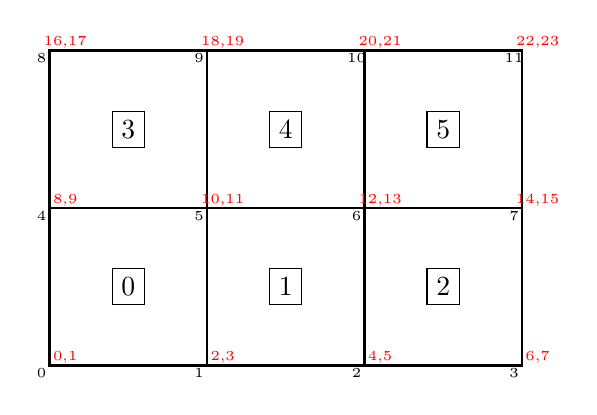
\begin{tikzpicture}
%\draw[step=0.5cm,gray,very thin] (0,0) grid (8,6); %background grid
\draw[thick] (1,1) -- (3,1) -- (3,3) -- (1,3) -- cycle;  
\draw[thick] (3,1) -- (5,1) -- (5,3) -- (3,3) -- cycle; 
\draw[thick] (5,1) -- (7,1) -- (7,3) -- (5,3) -- cycle; 
\draw[thick] (1,3) -- (3,3) -- (3,5) -- (1,5) -- cycle;  
\draw[thick] (3,3) -- (5,3) -- (5,5) -- (3,5) -- cycle; 
\draw[thick] (5,3) -- (7,3) -- (7,5) -- (5,5) -- cycle; 
\node[draw] at (2,2) {0};
\node[draw] at (4,2) {1};
\node[draw] at (6,2) {2};
\node[draw] at (2,4) {3};
\node[draw] at (4,4) {4};
\node[draw] at (6,4) {5};
%pressure dofs
\node at (0.9,0.9) {\tiny 0};
\node at (2.9,0.9) {\tiny 1};
\node at (4.9,0.9) {\tiny 2};
\node at (6.9,0.9) {\tiny 3};
\node at (0.9,2.9) {\tiny 4};
\node at (2.9,2.9) {\tiny 5};
\node at (4.9,2.9) {\tiny 6};
\node at (6.9,2.9) {\tiny 7};
\node at (0.9,4.9) {\tiny 8};
\node at (2.9,4.9) {\tiny 9};
\node at (4.9,4.9) {\tiny 10};
\node at (6.9,4.9) {\tiny 11};
%velocity dofs
\node[red] at (1.2,1.1) {\tiny 0,1};
\node[red] at (3.2,1.1) {\tiny 2,3};
\node[red] at (5.2,1.1) {\tiny 4,5};
\node[red] at (7.2,1.1) {\tiny 6,7};
\node[red] at (1.2,3.1) {\tiny 8,9};
\node[red] at (3.2,3.1) {\tiny 10,11};
\node[red] at (5.2,3.1) {\tiny 12,13};
\node[red] at (7.2,3.1) {\tiny 14,15};
\node[red] at (1.2,5.1) {\tiny 16,17};
\node[red] at (3.2,5.1) {\tiny 18,19};
\node[red] at (5.2,5.1) {\tiny 20,21};
\node[red] at (7.2,5.1) {\tiny 22,23};
\end{tikzpicture}
\end{center}




The $\K$ matrix is of size $NfemV \times NfemV$ with $NfemV=ndofV \times nnp = 2\times 12=24$.
The $\G$ matrix is of size $NfemV \times NfemP$ with $NfemP=ndofP \times nnp = 1\times 12=12$.
The $\C$ matrix is of size $NfemP \times NfemP$. 

A corner pdof sees 4 vdofs, a side pdof sees 12 vdofs and an inside pdof sees 18 vdofs, so that 
the total number of nonzeros in $\G$ can be computed as follows:
\[
NZ_\G = \underbrace{4}_{corners} + 
\underbrace{2(nnx-2)*12}_{2 hor. sides} 
+ 
\underbrace{2(nny-2)*12}_{2 vert. sides} 
+ 
\underbrace{(nnx-2)(nny-2)*18}_{inside nodes}
\]
Concretely, 
\begin{itemize}
\item pdof $\#0$ sees vdofs 0,1,2,3,8,9,10,11
\item pdof $\#1$ sees vdofs 0,1,2,3,4,5,8,9,10,11,12,13
\item pdof $\#5$ sees vdofs 0,1,2,3,4,5,8,9,10,11,12,13,16,17,18,19,20,21
\end{itemize}
so that the $\G^T$ matrix non-zero structure then is as follows:


\begin{center}
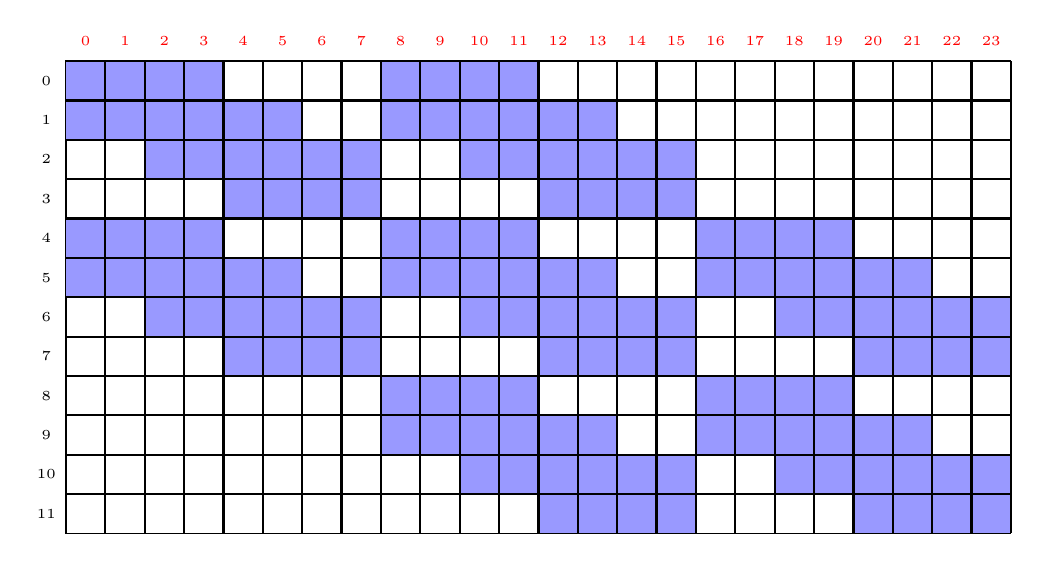
\begin{tikzpicture}
%\draw[step=0.5cm,gray,very thin] (0,0) grid (14,8); %background grid
\draw (1,1) -- (13,1) -- (13,7) -- (1,7) -- cycle;    %matrix
%first top line
\fill[blue!40!white] (1.0,6.5) rectangle (1.5,7);
\fill[blue!40!white] (1.5,6.5) rectangle (2.0,7);
\fill[blue!40!white] (2.0,6.5) rectangle (2.5,7);
\fill[blue!40!white] (2.5,6.5) rectangle (3.0,7);
\fill[blue!40!white] (5.0,6.5) rectangle (5.5,7);
\fill[blue!40!white] (5.5,6.5) rectangle (6.0,7);
\fill[blue!40!white] (6.0,6.5) rectangle (6.5,7);
\fill[blue!40!white] (6.5,6.5) rectangle (7.0,7);
%second line
\fill[blue!40!white] (1.0,6.) rectangle (1.5,6.5);
\fill[blue!40!white] (1.5,6.) rectangle (2.0,6.5);
\fill[blue!40!white] (2.0,6.) rectangle (2.5,6.5);
\fill[blue!40!white] (2.5,6.) rectangle (3.0,6.5);
\fill[blue!40!white] (3.0,6.) rectangle (3.5,6.5);
\fill[blue!40!white] (3.5,6.) rectangle (4.0,6.5);
\fill[blue!40!white] (5.0,6.) rectangle (5.5,6.5);
\fill[blue!40!white] (5.5,6.) rectangle (6.0,6.5);
\fill[blue!40!white] (6.0,6.) rectangle (6.5,6.5);
\fill[blue!40!white] (6.5,6.) rectangle (7.0,6.5);
\fill[blue!40!white] (7.0,6.) rectangle (7.5,6.5);
\fill[blue!40!white] (7.5,6.) rectangle (8.0,6.5);
%third line
\fill[blue!40!white] (2.0,5.5) rectangle (2.5,6.0);
\fill[blue!40!white] (2.5,5.5) rectangle (3.0,6.0);
\fill[blue!40!white] (3.0,5.5) rectangle (3.5,6.0);
\fill[blue!40!white] (3.5,5.5) rectangle (4.0,6.0);
\fill[blue!40!white] (4.0,5.5) rectangle (4.5,6.0);
\fill[blue!40!white] (4.5,5.5) rectangle (5.0,6.0);
\fill[blue!40!white] (6.0,5.5) rectangle (6.5,6.0);
\fill[blue!40!white] (6.5,5.5) rectangle (7.0,6.0);
\fill[blue!40!white] (7.0,5.5) rectangle (7.5,6.0);
\fill[blue!40!white] (7.5,5.5) rectangle (8.0,6.0);
\fill[blue!40!white] (8.0,5.5) rectangle (8.5,6.0);
\fill[blue!40!white] (8.5,5.5) rectangle (9.0,6.0);
%fourth line
\fill[blue!40!white] (3.0,5.) rectangle (3.5,5.5);
\fill[blue!40!white] (3.5,5.) rectangle (4.0,5.5);
\fill[blue!40!white] (4.0,5.) rectangle (4.5,5.5);
\fill[blue!40!white] (4.5,5.) rectangle (5.0,5.5);
\fill[blue!40!white] (7.0,5.) rectangle (7.5,5.5);
\fill[blue!40!white] (7.5,5.) rectangle (8.0,5.5);
\fill[blue!40!white] (8.0,5.) rectangle (8.5,5.5);
\fill[blue!40!white] (8.5,5.) rectangle (9.0,5.5);
%fifth line
\fill[blue!40!white] (1.0,4.5) rectangle (1.5,5);
\fill[blue!40!white] (1.5,4.5) rectangle (2.0,5);
\fill[blue!40!white] (2.0,4.5) rectangle (2.5,5);
\fill[blue!40!white] (2.5,4.5) rectangle (3.0,5);
\fill[blue!40!white] (5.0,4.5) rectangle (5.5,5);
\fill[blue!40!white] (5.5,4.5) rectangle (6.0,5);
\fill[blue!40!white] (6.0,4.5) rectangle (6.5,5);
\fill[blue!40!white] (6.5,4.5) rectangle (7.0,5);
\fill[blue!40!white] (9.0,4.5) rectangle (9.5,5);
\fill[blue!40!white] (9.5,4.5) rectangle (10.0,5);
\fill[blue!40!white] (10.0,4.5) rectangle (10.5,5);
\fill[blue!40!white] (10.5,4.5) rectangle (11.0,5);

%sixth line
\fill[blue!40!white] (1.0,4) rectangle (1.5,4.50);
\fill[blue!40!white] (1.5,4) rectangle (2.0,4.50);
\fill[blue!40!white] (2.0,4) rectangle (2.5,4.50);
\fill[blue!40!white] (2.5,4) rectangle (3.0,4.50);
\fill[blue!40!white] (3.0,4) rectangle (3.5,4.50);
\fill[blue!40!white] (3.5,4) rectangle (4.0,4.50);


\fill[blue!40!white] (5.0,4) rectangle (5.5,4.50);
\fill[blue!40!white] (5.5,4) rectangle (6.0,4.50);
\fill[blue!40!white] (6.0,4) rectangle (6.5,4.50);
\fill[blue!40!white] (6.5,4) rectangle (7.0,4.50);
\fill[blue!40!white] (7.0,4) rectangle (7.5,4.50);
\fill[blue!40!white] (7.5,4) rectangle (8.0,4.50);

\fill[blue!40!white] (9.0,4) rectangle (9.5,4.50);
\fill[blue!40!white] (9.5,4) rectangle (10.0,4.50);
\fill[blue!40!white] (10.0,4) rectangle (10.5,4.50);
\fill[blue!40!white] (10.5,4) rectangle (11.0,4.50);
\fill[blue!40!white] (11.0,4) rectangle (11.5,4.50);
\fill[blue!40!white] (11.5,4) rectangle (12.0,4.50);

%seventh line
\fill[blue!40!white] (2.0,3.5) rectangle (2.5,4.0);
\fill[blue!40!white] (2.5,3.5) rectangle (3.0,4.0);
\fill[blue!40!white] (3.0,3.5) rectangle (3.5,4.0);
\fill[blue!40!white] (3.5,3.5) rectangle (4.0,4.0);
\fill[blue!40!white] (4.0,3.5) rectangle (4.5,4.0);
\fill[blue!40!white] (4.5,3.5) rectangle (5.0,4.0);
\fill[blue!40!white] (6.0,3.5) rectangle (6.5,4.0);
\fill[blue!40!white] (6.5,3.5) rectangle (7.0,4.0);
\fill[blue!40!white] (7.0,3.5) rectangle (7.5,4.0);
\fill[blue!40!white] (7.5,3.5) rectangle (8.0,4.0);
\fill[blue!40!white] (8.0,3.5) rectangle (8.5,4.0);
\fill[blue!40!white] (8.5,3.5) rectangle (9.0,4.0);
\fill[blue!40!white] (10.0,3.5) rectangle (10.5,4.0);
\fill[blue!40!white] (10.5,3.5) rectangle (11.0,4.0);
\fill[blue!40!white] (11.0,3.5) rectangle (11.5,4.0);
\fill[blue!40!white] (11.5,3.5) rectangle (12.0,4.0);
\fill[blue!40!white] (12.0,3.5) rectangle (12.5,4.0);
\fill[blue!40!white] (12.5,3.5) rectangle (13.0,4.0);
%eighth line
\fill[blue!40!white] (3.0,3.) rectangle (3.5,3.5);
\fill[blue!40!white] (3.5,3.) rectangle (4.0,3.5);
\fill[blue!40!white] (4.0,3.) rectangle (4.5,3.5);
\fill[blue!40!white] (4.5,3.) rectangle (5.0,3.5);
\fill[blue!40!white] (7.0,3.) rectangle (7.5,3.5);
\fill[blue!40!white] (7.5,3.) rectangle (8.0,3.5);
\fill[blue!40!white] (8.0,3.) rectangle (8.5,3.5);
\fill[blue!40!white] (8.5,3.) rectangle (9.0,3.5);
\fill[blue!40!white] (11.0,3.) rectangle (11.5,3.5);
\fill[blue!40!white] (11.5,3.) rectangle (12.0,3.5);
\fill[blue!40!white] (12.0,3.) rectangle (12.5,3.5);
\fill[blue!40!white] (12.5,3.) rectangle (13.0,3.5);
%9th line
\fill[blue!40!white] (5.0,2.5) rectangle (5.5,3);
\fill[blue!40!white] (5.5,2.5) rectangle (6.0,3);
\fill[blue!40!white] (6.0,2.5) rectangle (6.5,3);
\fill[blue!40!white] (6.5,2.5) rectangle (7.0,3);
\fill[blue!40!white] (9.0,2.5) rectangle (9.5,3);
\fill[blue!40!white] (9.5,2.5) rectangle (10.0,3);
\fill[blue!40!white] (10.0,2.5) rectangle (10.5,3);
\fill[blue!40!white] (10.5,2.5) rectangle (11.0,3);
%10th line
\fill[blue!40!white] (5.0,2) rectangle (5.5,2.5);
\fill[blue!40!white] (5.5,2) rectangle (6.0,2.5);
\fill[blue!40!white] (6.0,2) rectangle (6.5,2.5);
\fill[blue!40!white] (6.5,2) rectangle (7.0,2.5);
\fill[blue!40!white] (7.0,2) rectangle (7.5,2.5);
\fill[blue!40!white] (7.5,2) rectangle (8.0,2.5);
\fill[blue!40!white] (9.0,2) rectangle (9.5,2.5);
\fill[blue!40!white] (9.5,2) rectangle (10.0,2.5);
\fill[blue!40!white] (10.0,2) rectangle (10.5,2.5);
\fill[blue!40!white] (10.5,2) rectangle (11.0,2.5);
\fill[blue!40!white] (11.0,2) rectangle (11.5,2.5);
\fill[blue!40!white] (11.5,2) rectangle (12.0,2.5);
%11th line
\fill[blue!40!white] (6.0,1.5) rectangle (6.5,2);
\fill[blue!40!white] (6.5,1.5) rectangle (8,2);
\fill[blue!40!white] (7.0,1.5) rectangle (7.5,2);
\fill[blue!40!white] (7.5,1.5) rectangle (8.0,2);
\fill[blue!40!white] (8.0,1.5) rectangle (8.5,2);
\fill[blue!40!white] (8.5,1.5) rectangle (9.0,2);
\fill[blue!40!white] (10.0,1.5) rectangle (10.5,2);
\fill[blue!40!white] (10.5,1.5) rectangle (11.0,2);
\fill[blue!40!white] (11.0,1.5) rectangle (11.5,2);
\fill[blue!40!white] (11.5,1.5) rectangle (12.0,2);
\fill[blue!40!white] (12.0,1.5) rectangle (12.5,2);
\fill[blue!40!white] (12.5,1.5) rectangle (13.0,2);
%12th line
\fill[blue!40!white] (7.0,1.0) rectangle (7.5,1.5);
\fill[blue!40!white] (7.5,1.0) rectangle (8.0,1.5);
\fill[blue!40!white] (8.0,1.0) rectangle (8.5,1.5);
\fill[blue!40!white] (8.5,1.0) rectangle (9.0,1.5);
\fill[blue!40!white] (11.0,1.0) rectangle (11.5,1.5);
\fill[blue!40!white] (11.5,1.0) rectangle (12.0,1.5);
\fill[blue!40!white] (12.0,1.0) rectangle (12.5,1.5);
\fill[blue!40!white] (12.5,1.0) rectangle (13.0,1.5);
%vertical
\node at (0.75,6.75) {\tiny 0};
\node at (0.75,6.25) {\tiny 1};
\node at (0.75,5.75) {\tiny 2};
\node at (0.75,5.25) {\tiny 3};
\node at (0.75,4.75) {\tiny 4};
\node at (0.75,4.25) {\tiny 5};
\node at (0.75,3.75) {\tiny 6};
\node at (0.75,3.25) {\tiny 7};
\node at (0.75,2.75) {\tiny 8};
\node at (0.75,2.25) {\tiny 9};
\node at (0.75,1.75) {\tiny 10};
\node at (0.75,1.25) {\tiny 11};
%horizontal
\node[red] at (1.25,7.25) {\tiny 0};
\node[red] at (1.75,7.25) {\tiny 1};
\node[red] at (2.25,7.25) {\tiny 2};
\node[red] at (2.75,7.25) {\tiny 3};
\node[red] at (3.25,7.25) {\tiny 4};
\node[red] at (3.75,7.25) {\tiny 5};
\node[red] at (4.25,7.25) {\tiny 6};
\node[red] at (4.75,7.25) {\tiny 7};
\node[red] at (5.25,7.25) {\tiny 8};
\node[red] at (5.75,7.25) {\tiny 9};
\node[red] at (6.25,7.25) {\tiny 10};
\node[red] at (6.75,7.25) {\tiny 11};
\node[red] at (7.25,7.25) {\tiny 12};
\node[red] at (7.75,7.25) {\tiny 13};
\node[red] at (8.25,7.25) {\tiny 14};
\node[red] at (8.75,7.25) {\tiny 15};
\node[red] at (9.25,7.25) {\tiny 16};
\node[red] at (9.75,7.25) {\tiny 17};
\node[red] at (10.25,7.25) {\tiny 18};
\node[red] at (10.75,7.25) {\tiny 19};
\node[red] at (11.25,7.25) {\tiny 20};
\node[red] at (11.75,7.25) {\tiny 21};
\node[red] at (12.25,7.25) {\tiny 22};
\node[red] at (12.75,7.25) {\tiny 23};
\draw[step=0.5cm,black,thick] (1,1) grid (13,7); %background grid
\end{tikzpicture}
\end{center}










%-------------------------------------------------------------
\subsection*{Non-zero pattern of the $\C$ matrix}

Concretely, 
\begin{itemize}
\item pdof $\#0$ sees vdofs 0,1,4,5
\item pdof $\#1$ sees vdofs 0,1,2,4,5,6
\item pdof $\#5$ sees vdofs 0,1,2,4,5,6,8,9,10
\end{itemize}
so that the $\C$ matrix non-zero structure is as follows:


\begin{center}
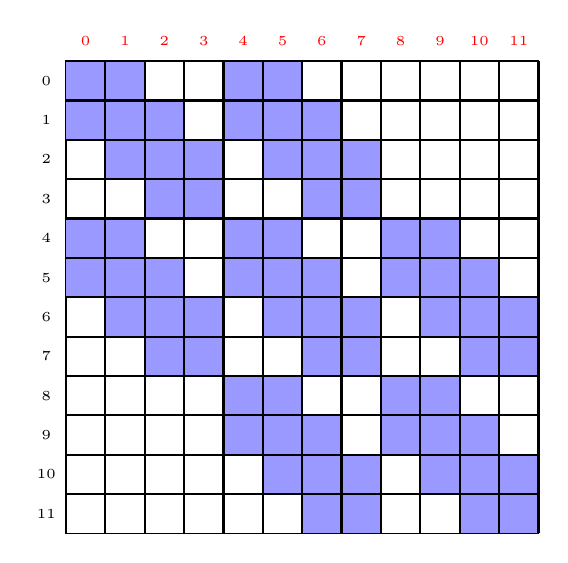
\begin{tikzpicture}
%\draw[step=0.5cm,gray,very thin] (0,0) grid (9,9); %background grid
\draw (1,1) -- (7,1) -- (7,7) -- (1,7) -- cycle;    %matrix

%vertical
\node at (0.75,6.75) {\tiny 0};
\node at (0.75,6.25) {\tiny 1};
\node at (0.75,5.75) {\tiny 2};
\node at (0.75,5.25) {\tiny 3};
\node at (0.75,4.75) {\tiny 4};
\node at (0.75,4.25) {\tiny 5};
\node at (0.75,3.75) {\tiny 6};
\node at (0.75,3.25) {\tiny 7};
\node at (0.75,2.75) {\tiny 8};
\node at (0.75,2.25) {\tiny 9};
\node at (0.75,1.75) {\tiny 10};
\node at (0.75,1.25) {\tiny 11};

%horizontal
\node[red] at (1.25,7.25) {\tiny 0};
\node[red] at (1.75,7.25) {\tiny 1};
\node[red] at (2.25,7.25) {\tiny 2};
\node[red] at (2.75,7.25) {\tiny 3};
\node[red] at (3.25,7.25) {\tiny 4};
\node[red] at (3.75,7.25) {\tiny 5};
\node[red] at (4.25,7.25) {\tiny 6};
\node[red] at (4.75,7.25) {\tiny 7};
\node[red] at (5.25,7.25) {\tiny 8};
\node[red] at (5.75,7.25) {\tiny 9};
\node[red] at (6.25,7.25) {\tiny 10};
\node[red] at (6.75,7.25) {\tiny 11};

%first top line
\fill[blue!40!white] (1.0,6.5) rectangle (1.5,7);
\fill[blue!40!white] (1.5,6.5) rectangle (2.0,7);
\fill[blue!40!white] (3.0,6.5) rectangle (3.5,7);
\fill[blue!40!white] (3.5,6.5) rectangle (4.0,7);
%second line
\fill[blue!40!white] (1.0,6.) rectangle (1.5,6.5);
\fill[blue!40!white] (1.5,6.) rectangle (2.0,6.5);
\fill[blue!40!white] (2.0,6.) rectangle (2.5,6.5);
\fill[blue!40!white] (3.0,6.) rectangle (3.5,6.5);
\fill[blue!40!white] (3.5,6.) rectangle (4.0,6.5);
\fill[blue!40!white] (4.0,6.) rectangle (4.5,6.5);
%third line
\fill[blue!40!white] (1.5,5.5) rectangle (2.0,6.);
\fill[blue!40!white] (2.0,5.5) rectangle (2.5,6.);
\fill[blue!40!white] (2.5,5.5) rectangle (3.0,6.);
\fill[blue!40!white] (3.5,5.5) rectangle (4.0,6.);
\fill[blue!40!white] (4.0,5.5) rectangle (4.5,6.);
\fill[blue!40!white] (4.5,5.5) rectangle (5.0,6.);
%fourth line
\fill[blue!40!white] (2.0,5.) rectangle (2.5,5.5);
\fill[blue!40!white] (2.5,5.) rectangle (3.0,5.5);
\fill[blue!40!white] (4.0,5.) rectangle (4.5,5.5);
\fill[blue!40!white] (4.5,5.) rectangle (5.0,5.5);
%fifth line
\fill[blue!40!white] (1.0,4.5) rectangle (1.5,5.);
\fill[blue!40!white] (1.5,4.5) rectangle (2.0,5.);
\fill[blue!40!white] (3.0,4.5) rectangle (3.5,5.);
\fill[blue!40!white] (3.5,4.5) rectangle (4.0,5.);
\fill[blue!40!white] (5.0,4.5) rectangle (5.5,5.);
\fill[blue!40!white] (5.5,4.5) rectangle (6.0,5.);
%sixth line
\fill[blue!40!white] (1.0,4.) rectangle (1.5,4.5);
\fill[blue!40!white] (1.5,4.) rectangle (2.0,4.5);
\fill[blue!40!white] (2.0,4.) rectangle (2.5,4.5);
\fill[blue!40!white] (3.0,4.) rectangle (3.5,4.5);
\fill[blue!40!white] (3.5,4.) rectangle (4.0,4.5);
\fill[blue!40!white] (4.0,4.) rectangle (4.5,4.5);
\fill[blue!40!white] (5.0,4.) rectangle (5.5,4.5);
\fill[blue!40!white] (5.5,4.) rectangle (6.0,4.5);
\fill[blue!40!white] (6.0,4.) rectangle (6.5,4.5);
%seventh line
\fill[blue!40!white] (1.5,3.5) rectangle (2.0,4.);
\fill[blue!40!white] (2.0,3.5) rectangle (2.5,4.);
\fill[blue!40!white] (2.5,3.5) rectangle (3.0,4.);
\fill[blue!40!white] (3.5,3.5) rectangle (4.0,4.);
\fill[blue!40!white] (4.0,3.5) rectangle (4.5,4.);
\fill[blue!40!white] (4.5,3.5) rectangle (5.0,4.);
\fill[blue!40!white] (5.5,3.5) rectangle (6.0,4.);
\fill[blue!40!white] (6.0,3.5) rectangle (6.5,4.);
\fill[blue!40!white] (6.5,3.5) rectangle (7.0,4.);
%eighth line
\fill[blue!40!white] (2.0,3.) rectangle (2.5,3.5);
\fill[blue!40!white] (2.5,3.) rectangle (3.0,3.5);
\fill[blue!40!white] (4.0,3.) rectangle (4.5,3.5);
\fill[blue!40!white] (4.5,3.) rectangle (5.0,3.5);
\fill[blue!40!white] (6.0,3.) rectangle (6.5,3.5);
\fill[blue!40!white] (6.5,3.) rectangle (7.0,3.5);
%ninth line
\fill[blue!40!white] (3.0,2.5) rectangle (3.5,3.);
\fill[blue!40!white] (3.5,2.5) rectangle (4.0,3.);
\fill[blue!40!white] (5.0,2.5) rectangle (5.5,3.);
\fill[blue!40!white] (5.5,2.5) rectangle (6.0,3.);
%tenth line
\fill[blue!40!white] (3.0,2.) rectangle (3.5,2.5);
\fill[blue!40!white] (3.5,2.) rectangle (4.0,2.5);
\fill[blue!40!white] (4.0,2.) rectangle (4.5,2.5);
\fill[blue!40!white] (5.0,2.) rectangle (5.5,2.5);
\fill[blue!40!white] (5.5,2.) rectangle (6.0,2.5);
\fill[blue!40!white] (6.0,2.) rectangle (6.5,2.5);
%eleventh line
\fill[blue!40!white] (3.5,1.5) rectangle (4.0,2.);
\fill[blue!40!white] (4.0,1.5) rectangle (4.5,2.);
\fill[blue!40!white] (4.5,1.5) rectangle (5.0,2.);
\fill[blue!40!white] (5.5,1.5) rectangle (6.0,2.);
\fill[blue!40!white] (6.0,1.5) rectangle (6.5,2.);
\fill[blue!40!white] (6.5,1.5) rectangle (7.0,2.);
%twelfth line
\fill[blue!40!white] (4.0,1.) rectangle (4.5,1.5);
\fill[blue!40!white] (4.5,1.) rectangle (5.0,1.5);
\fill[blue!40!white] (6.0,1.) rectangle (6.5,1.5);
\fill[blue!40!white] (6.5,1.) rectangle (7.0,1.5);


\draw[step=0.5cm,black,thick] (1,1) grid (7,7); %background grid





\end{tikzpicture}
\end{center}





%-------------------------------------------------------------
\subsection*{Constraining the pressure field to zero average}

We impose $\int p dV=0$ which means that the following constraint is added 
to the Stokes matrix:
\[
\left(
\begin{array}{ccc}
\K & \G & 0\\ 
\G^T & \C & \LLL \\
0 & \LLL^T & 0 
\end{array}
\right)
\cdot
\left(
\begin{array}{c}
{\cal V} \\ {\cal P} \\ \lambda
\end{array}
\right)
=
\left(
\begin{array}{c}
 f \\ h \\ 0
\end{array}
\right)
\]




%---------------------------------------------------
\subsection*{The Donea \& Huerta benchmark (case 1)}

As in \cite{dohu03} we solve the benchmark problem presented in section \ref{mms1}.

\begin{center}
\includegraphics[width=10cm]{python_codes/fieldstone_22/results/case1/errors.pdf}
\end{center}

%------------------------------------------------------
\subsection*{The Dohrmann \& Bochev benchmark (case 2)} 

As in \cite{dobo04} we solve the benchmark problem presented in section \ref{mms2}.

\begin{center}
\includegraphics[width=10cm]{python_codes/fieldstone_22/results/case2/errors.pdf}
\end{center}

\todo[inline]{compare my rates with original paper!}

%\includegraphics[width=5cm]{python_codes/fieldstone_22/results/uth}
%\includegraphics[width=5cm]{python_codes/fieldstone_22/results/vth}
%\includegraphics[width=5cm]{python_codes/fieldstone_22/results/pth}

%--------------------------------------------------
\subsection*{The sinking block experiment (case 3)} 

The setup is described in \cite{thba20}. 
It consists of a two-dimensional $512\times 512$km domain filled with a fluid (the "mantle") 
of density $\rho_1=3200$kg/m$^3$ and viscosity $\eta_1$. A square block of 
size $128\times 128$km is placed in the domain and is centered at location 
($x_c,y_c$)=(256km,384km) so as to insure that its sides align with cell boundaries at 
all resolutions. It is filled with a fluid of density $\rho_2=\rho_1+\delta \rho$ 
and viscosity $\eta_2$. The gravity vector points downwards with $|\vec{g}|=10$m/s$^2$. 
Boundary conditions are free slip on all sides. Only one time step is carried out and 
we measure the velocity $|v_z|$ in the middle of the block. 

\begin{center}
\includegraphics[width=13cm]{python_codes/fieldstone_22/results/case3/blocks}
\end{center}

\begin{center}
\includegraphics[width=5cm]{python_codes/fieldstone_22/results/case3/fallingblock_sub1.pdf}
\includegraphics[width=5cm]{python_codes/fieldstone_22/results/case3/fallingblock_sub2.pdf}
\includegraphics[width=5cm]{python_codes/fieldstone_22/results/case3/fallingblock_sub3.pdf}\\
{\captionfont From left to right: subcase=1,2,3.}
\end{center}

\begin{center}
\includegraphics[width=12cm]{python_codes/fieldstone_22/results/case3/u123}
\includegraphics[width=12cm]{python_codes/fieldstone_22/results/case3/v123}\\
{\captionfont From left to right: subcase=1,2,3. 
Resolution 96x96, $\delta \rho=32$, $\eta_2=10^{23}$}
\end{center}





%-----------------------------------------
\subsection*{SolCx (case 4)} 

This benchmark is described in Section~\ref{mms:solcx}.

\begin{center}
\includegraphics[width=10cm]{python_codes/fieldstone_22/results/case4/errors.pdf}\\
{\captionfont Resolutions 8x8 to 96x96. Even resolutions converge ${\cal O}(h^2)$ 
for velocity while \\ even resolutions converge ${\cal O}(h^1)$. In both cases the \\
pressure converges ${\cal O}(h^{1/2})$.}
\end{center}


%-----------------------------------------
\subsection*{SolVi (case 5)} 

This benchmark is described in Section~\ref{mms:solvi}.

\begin{center}
\includegraphics[width=10cm]{python_codes/fieldstone_22/results/case5/errors.pdf}\\
{\captionfont Resolutions 8x8 to 96x96.} 
\end{center}

\begin{center}
\includegraphics[width=7cm]{python_codes/fieldstone_22/results/case5/veldiag}
\includegraphics[width=7cm]{python_codes/fieldstone_22/results/case5/pressbottom}\\
{\captionfont Velocity and pressure on the diagonal $y=x$, at resolution 96x96.} 
\end{center}

\begin{center}
\includegraphics[width=5cm]{python_codes/fieldstone_22/results/case5/vel}
\includegraphics[width=5cm]{python_codes/fieldstone_22/results/case5/vel2}
\includegraphics[width=5cm]{python_codes/fieldstone_22/results/case5/p}\\
\end{center}





\newpage %%%%%%%%%%%%%%%%%%%%%%%%%%%%%%%%%%%%%%%%%%%%%%%%%%%%%%%%%%%%%%%%%%%%%%%%%%%%%%%%
\section*{
Stone 23: compressible flow (1) - analytical benchmark 
\label{f23}}
\addcontentsline{toc}{section}{\protect\numberline{} 
Stone 23: compressible flow (1) - analytical benchmark 
}

\index{stones}{$Q_1 \times P_0$ element}
\index{stones}{Mixed Formulation}
\index{stones}{Analytical Solution}
\index{stones}{Pressure Smoothing} 

\begin{mdframed}[backgroundcolor=red!5]
This work is part of the MSc thesis of T. Weir (2018).
\end{mdframed}
\index{contributors}{T. Weir}

We first start with an isothermal Stokes flow, so that we disregard the heat transport equation and 
the equations we wish to solve are simply:

\begin{align}
  \label{eq:stokes-1}
  -\nabla \cdot \left[2\eta \left(\dot\varepsilon(\bm v)
                                  - \frac{1}{3}(\nabla \cdot \bm v)\mathbf 1\right)
                \right] + \nabla p &=
  \rho \bm g
  &
  & \textrm{in $\Omega$},
  \\
  \label{eq:stokes-2}
  \nabla \cdot (\rho \bm v) &= 0
  &
  & \textrm{in $\Omega$}
\end{align}
The second equation can be rewritten 
$\nabla \cdot (\rho {\bm v}) =  \rho \nabla \cdot {\bm v} + {\bm v} \cdot {\bm \nabla}\rho=0$
or, 
\[
\nabla \cdot {\bm v} + \frac{1}{\rho} {\bm v} \cdot {\bm \nabla}\rho=0
\]
Note that this presupposes that the density is not zero anywhere in the domain.

We use a mixed formulation and therefore  
keep both velocity and pressure as unknowns. We end up having to solve 
the following system:
\[
\left(
\begin{array}{cc}
\K & \G \\ \G^T+\Z & 0 
\end{array}
\right)
\cdot
\left(
\begin{array}{c}
{\cal V} \\ {\cal P}
\end{array}
\right)
=
\left(
\begin{array}{c}
 f \\ h
\end{array}
\right)
\quad\quad
{\rm or,}
\quad\quad
\A \cdot X = rhs
\]
Where $\K$ is the stiffness matrix, $\G$ is the discrete gradient operator, 
$\G^T$ is the discrete divergence operator, ${\cal V}$ the velocity vector, 
${\cal P}$ the pressure vector.
Note that the term $\Z{\cal V}$ derives from term ${\bm v} \cdot {\bm \nabla} \rho$ in the continuity equation. 

Each block $\K$, $\G$ , $\Z$ and vectors $f$ and $h$ are built separately 
in the code and assembled into 
the matrix $\A$ and vector $rhs$ afterwards. $\A$ and $rhs$ are then passed to the solver. 
We will see later that there are alternatives to solve this approach which do not require to 
build the full Stokes matrix $\A$. 

{\sl Remark}: the term $\Z {\cal V}$ is often put in the rhs (i.e. added to $h$) so that 
the matrix $\A$ retains the same structure as in the incompressible case. This is indeed 
how it is implemented in ASPECT. This however requires more work since the rhs depends 
on the solution and some form of iterations is needed. 

In the case of a compressible flow the strain rate tensor and the deviatoric strain rate tensor are no more equal (since ${\bm \nabla}\cdot{\bm v} \neq 0$).
The deviatoric strainrate tensor is given by\footnote{See the ASPECT manual for a justification of the 3 value in the denominator in 2D and 3D.} 
\[
\dot{\bm \epsilon}^d({\bm v})=
\dot{\bm \epsilon}({\bm v})-\frac{1}{3} Tr(\dot{\bm \epsilon}) {\bm 1}
=\dot{\bm \epsilon}({\bm v})-\frac{1}{3} ({\bm \nabla}\cdot{\bm v}) {\bm 1}
\]
In that case:
\begin{eqnarray}
\dot{\epsilon}_{xx}^d 
&=& \frac{\partial u}{\partial x}
-\frac{1}{3} \left( \frac{\partial u}{\partial x} + \frac{\partial v}{\partial y} \right) 
= \frac{2}{3}\frac{\partial u}{\partial x}
-\frac{1}{3} \frac{\partial v}{\partial y}
%=
%\frac{2}{3} \sum_{i=1}^4 \frac{\partial N_i}{\partial x}\;  u_i 
%-\frac{1}{3} \sum_{i=1}^4 \frac{\partial N_i}{\partial y}\;  v_i 
\\
\dot{\epsilon}_{yy}^d 
&=& \frac{\partial v}{\partial y}
-\frac{1}{3} \left( \frac{\partial u}{\partial x} + \frac{\partial v}{\partial y} \right) 
=-\frac{1}{3} \frac{\partial u}{\partial x} 
+ \frac{2}{3} \frac{\partial v}{\partial y} 
%=-\frac{1}{3}  \sum_{i=1}^4 \frac{\partial N_i}{\partial x}\;  u_i
%+ \frac{2}{3} \sum_{i=1}^4 \frac{\partial N_i}{\partial y}\;  v_i
\\
2\dot{\epsilon}_{xy}^d 
&=& 
\frac{\partial u}{\partial y} 
+\frac{\partial v}{\partial x} 
%= \sum_{i=1}^4 \frac{\partial N_i}{\partial y}\;  u_i
%+ \sum_{i=1}^4 \frac{\partial N_i}{\partial x}\;  v_i
\end{eqnarray}
and then 
\[
\dot{\bm \epsilon}^d({\bm v})
=
\left(
\begin{array}{cc}
\frac{2}{3} \frac{\partial u}{\partial x} -\frac{1}{3} \frac{\partial v}{\partial y} &
\frac{1}{2}\frac{\partial u}{\partial y} + \frac{1}{2}\frac{\partial v}{\partial x}  \\ \\
\frac{1}{2}\frac{\partial u}{\partial y} + \frac{1}{2}\frac{\partial v}{\partial x}  &
-\frac{1}{3} \frac{\partial u}{\partial x} +\frac{2}{3} \frac{\partial v}{\partial y} 
\end{array}
\right)
\]

From $\vec{\tau} = 2\eta \vec{\epsilon}^d$ we arrive at:
\[
\left(
\begin{array}{c}
\tau_{xx}\\
\tau_{yy}\\
\tau_{xy}\\
\end{array}
\right)
=
2\eta
\left(
\begin{array}{c}
\dot{\epsilon}_{xx}^d \\
\dot{\epsilon}_{yy}^d \\
\dot{\epsilon}_{xy}^d 
\end{array}
\right)
=2 \eta
\left(
\begin{array}{ccc}
2/3 & -1/3& 0 \\
-1/3 & 2/3 & 0 \\
0 & 0 & 1/2 \\
\end{array}
\right)
\cdot 
\left(
\begin{array}{c}
\frac{\partial u}{\partial x} \\ 
\frac{\partial v}{\partial y} \\ 
\frac{\partial u}{\partial y}\! +\! \frac{\partial v}{\partial x} \\
\end{array}
\right)
=
\eta
\left(
\begin{array}{ccc}
4/3 & -2/3& 0 \\
-2/3 & 4/3 & 0 \\
0 & 0 & 1 \\
\end{array}
\right)
\cdot 
\left(
\begin{array}{c}
\frac{\partial u}{\partial x} \\ 
\frac{\partial v}{\partial y} \\ 
\frac{\partial u}{\partial y}\! +\! \frac{\partial v}{\partial x} \\
\end{array}
\right)
\]
or, 
\[
\vec{\tau} = {\bm C}_\eta {\bm B} V
\]


















\newpage
In order to test our implementation we have created a few manufactured solutions:
\begin{itemize}
\item \underline{benchmark \#1} ({\tt ibench=1})): Starting from a density profile of:
\begin{equation}
    \rho(x,y) = xy
\end{equation}
We derive a velocity given by:
\begin{equation}
    v_x(x,y) = \frac{C_x}{x} , v_y(x,y) = \frac{C_y}{y}
\end{equation}

With $g_x(x,y) = \frac{1}{x}$ and $g_y(x,y) = \frac{1}{y}$, this leads us to a pressure profile:
\begin{equation}
    p = - \eta \left( \frac{4C_x}{3x^2} + \frac{4C_y}{3y^2} \right)  + xy + C_0
\end{equation}
This gives us a strain rate:
\[
\dot{\epsilon}_{xx} =  \frac{-C_x}{x^2}
\quad
\quad
\quad
\dot{\epsilon}_{yy} =  \frac{-C_y}{y^2}
\quad
\quad
\quad
\dot{\epsilon}_{xy} = 0 
\]
In what follows, we choose $\eta=1$ and $C_x=C_y=1$ and for a unit square domain $
[1:2]\times[1:2]$ we compute $C_0$
so that the pressure is normalised to zero over the whole domain and obtain $C_0=-1$. 
 
\item \underline{benchmark \#2} ({\tt ibench=2}): Starting from a density profile of:
\begin{equation}
    \rho = \cos(x)\cos(y)
\end{equation}
We derive a velocity given by:
\begin{equation}
    v_x = \frac{C_x}{\cos(x)} , v_y = \frac{C_y}{\cos(y)}
\end{equation}
With $g_x = \frac{1}{\cos(y)}$ and $g_y = \frac{1}{\cos(x)}$, this leads us to a pressure profile:
\begin{equation}
    p =  \eta \Bigg(\frac{4C_x \sin(x)}{3\cos^2(x)} + \frac{4C_y \sin(y)}{3\cos^2(y)}\Bigg) 
    +( \sin(x) + \sin(y) ) + C_0
\end{equation}
\[
\dot{\epsilon}_{xx} = C_x \frac{\sin(x)}{\cos^2(x)}
\quad
\quad
\quad
\dot{\epsilon}_{yy} = C_y \frac{\sin(y)}{\cos^2(y)}
\quad
\quad
\quad
\dot{\epsilon}_{xy} = 0 
\]
We choose $\eta=1$ and $C_x=C_y=1$. The domain is the unit square $[0:1]\times[0:1]$ and we obtain 
$C_0$ as before and obtain 
\[
C_0 = 2 - 2 \cos(1) + 8/3 (\frac{1}{\cos (1)} - 1)
\simeq 3.18823730
\]
(thank you WolframAlpha)


\item \underline{benchmark \#3} ({\tt ibench=3}) 
\item \underline{benchmark \#4} ({\tt ibench=4}) 
\item \underline{benchmark \#5} ({\tt ibench=5}) 
\end{itemize}





%\includegraphics[width=16cm]{python_codes/fieldstone_saddlepoint/solution.pdf}

ToDo:
\begin{itemize}
\item pbs with odd vs even number of elements 
\item q is 'fine' everywhere except in the corners - revisit pressure smoothing paper?
\item redo A v d Berg benchmark (see Tom Weir thesis)
\end{itemize}




\newpage %%%%%%%%%%%%%%%%%%%%%%%%%%%%%%%%%%%%%%%%%%%%%%%%%%%%%%%%%%%%%%%%%%%%%%%%%%%%%%%%
\section*{
Stone 24: compressible flow (2) - convection box 
\label{f24}}
\addcontentsline{toc}{section}{\protect\numberline{} 
Stone 24: compressible flow (2) - convection box 
}
\begin{mdframed}[backgroundcolor=red!5]
This work is part of the MSc thesis of T. Weir (2018).
\end{mdframed}


\subsection*{The physics}

Let us start with some thermodynamics. Every material has an equation of state.
The equilibrium thermodynamic state of any material can
be constrained if any two state variables are specified.
Examples of state variables include
the pressure $p$ and specific volume $\nu = 1/\rho$, as well as the temperature $T$.

After linearisation, the density depends on temperature and pressure as follows:
\[
\rho(T,p) = \rho_0 \left((1 - \alpha(T-T_0) + \beta_T p \right)
\]
where $\alpha$ is the coefficient of thermal expansion, also called 
thermal expansivity: \index{thermal expansion}
\[
\alpha=-\frac{1}{\rho}\left( \frac{\partial \rho}{\partial T} \right)_p
\]
$\alpha$ is the percentage increase in volume of a material per degree of temperature increase; the
subscript $p$ means that the pressure is held fixed.

$\beta_T$ is the isothermal compressibility of the fluid, which is given by \index{compressibility}
\[
\beta_T = \frac{1}{K} = \frac{1}{\rho}\left( \frac{\partial \rho}{\partial P} \right)_T
\]
with $K$ the bulk modulus. \index{bulk modulus}
%aspect manual
Values of $\beta_T=10^{-12}-10^{-11}$ Pa$^{-1}$ are reasonable for Earth's mantle, with values decreasing by about a
factor of 5 between the shallow lithosphere and core-mantle boundary.
This is the percentage increase in density per unit change in pressure at constant temperature.
Both the coefficient of thermal expansion and the isothermal compressibility can be obtained
from the equation of state.

The full set of equations we wish to solve is given by

\begin{eqnarray}
-\nabla \cdot \left[2\eta \dot{\bm \epsilon}^d({\bm v}) \right] + \nabla p &=& \rho_0 \left((1 - \alpha(T-T_0) + \beta_T p \right) {\bm g} \quad\quad \textrm{in $\Omega$}  \label{eq:stokes-1} \\
\nabla \cdot {\bm v} + \frac{1}{\rho} {\bm v} \cdot {\bm \nabla}\rho&=&0 \quad\quad  \textrm{in $\Omega$}   \label{eq:stokes-2} \\
\rho C_p \left(\frac{\partial T}{\partial t} + \bm v\cdot\nabla T\right) - \nabla\cdot k\nabla T   &=& 
  \rho H  +  2\eta \dot{\bm \epsilon}^d : \dot{\bm \epsilon}^d    +\alpha T \left( \frac{\partial p}{\partial t}+  \bm v \cdot \nabla p \right) 
\quad\quad   \textrm{in $\Omega$},
  \label{eq:temperature}
\end{eqnarray}

Note that this presupposes that the density is not zero anywhere in the domain.


\subsection*{The numerics}

We use a mixed formulation and therefore  
keep both velocity and pressure as unknowns. We end up having to solve 
the following system:
\[
\left(
\begin{array}{cc}
\K & \G+\W \\ \G^T+\Z & 0 
\end{array}
\right)
\cdot
\left(
\begin{array}{c}
{\cal V} \\ {\cal P}
\end{array}
\right)
=
\left(
\begin{array}{c}
 f \\ h
\end{array}
\right)
\quad\quad
{\rm or,}
\quad\quad
\A \cdot X = rhs
\]
Where $\K$ is the stiffness matrix, $\G$ is the discrete gradient operator, 
$\G^T$ is the discrete divergence operator, ${\cal V}$ the velocity vector, 
${\cal P}$ the pressure vector.
Note that the term $\Z{\cal V}$ derives from term ${\bm v} \cdot {\bm \nabla} \rho$ in the continuity equation. 

As perfectly explained in the step 32 of deal.ii\footnote{https://www.dealii.org/9.0.0/doxygen/deal.II/step\_32.html},
we need to scale the $\G$ term since it is many orders of magnitude smaller than $\K$, which introduces large inaccuracies in the solving process to the point that the solution is nonsensical. This scaling coefficient is $\eta/L$. After building the $\G$ block, it is then scaled as follows: $\G'=\frac{\eta}{L}\G$ so that we now solve 

\[
\left(
\begin{array}{cc}
\K & \G'+\W \\ \G'^T+\Z & 0 
\end{array}
\right)
\cdot
\left(
\begin{array}{c}
{\cal V} \\ {\cal P}'
\end{array}
\right)
=
\left(
\begin{array}{c}
 f \\ h
\end{array}
\right)
\]
After the solve phase, we recover the real pressure with ${\cal P}=\frac{\eta}{L}{\cal P}'$.

{\color{red} adapt notes since I should scale $\W$ and $\Z$ too}.
{\color{red} $h$ should be caled too !!!!!!!!!!!!!!!} 

Each block $\K$, $\G$ , $\Z$ and vectors $f$ and $h$ are built separately 
in the code and assembled into 
the matrix $\A$ and vector $rhs$ afterwards. $\A$ and $rhs$ are then passed to the solver. 
We will see later that there are alternatives to solve this approach which do not require to 
build the full Stokes matrix $\A$. 

{\bf Remark 1}: the terms $\Z {\cal V}$ and $\W {\cal P}$ are 
often put in the rhs (i.e. added to $h$) so that 
the matrix $\A$ retains the same structure as in the incompressible case. This is indeed 
how it is implemented in ASPECT, see also appendix A of \cite{lezh08}. This however requires more work since the rhs depends 
on the solution and some form of iterations is needed. 

{\bf Remark 2}: Very often the adiabatic heating term  
$\alpha T \left( \bm v \cdot \nabla p \right)$ is simplified as follows:
%aspect manual
If you assume the vertical component of the gradient of the dynamic pressure to be small compared to the
gradient of the total pressure (in other words, the gradient is dominated by the gradient of the hydrostatic
pressure), then $-\rho {\bm g} \simeq {\bm \nabla}p$ and then 
$\alpha T \left( \bm v \cdot \nabla p \right) \simeq  -\alpha\rho T {\bm v}\cdot{\bm g}$. We will however 
not be using this approximation in what follows.



We have already established that
\[
\vec{\tau} = {\bm C}_\eta {\bm B} V
\]


The following measurements are carried out:
\begin{itemize}
\item The root mean square velocity ({\tt vrms}):
\[
v_{rms} = \sqrt{\frac{1}{V}\int_V v^2 dV   }
\]
\item The average temperature ({\tt Tavrg}):
\[
<T>=\frac{1}{V}\int_V T dV
\]
\item The total mass ({\tt mass}):
\[
M=\int_V \rho dV 
\]
\item The Nusselt number ({\tt Nu}):
\[
Nu=-\frac{1}{Lx}\frac{1}{\Delta T} \int_0^{L_x} \frac{\partial T(x,y=L_y)}{\partial y} dx
\]
\item The kinetic energy ({\tt EK}):
\[
E_K=\int_V \frac{1}{2}\rho v^2 dV
\]
\item The work done against gravity 
\[
<W>=-\int_V \rho g_y v_y dV
\]
\item The total viscous dissipation ({\tt visc\_diss})
\[
<\Phi>=\int \Phi dV =\frac{1}{V}\int 2 \eta \dot{\bm \varepsilon}:\dot{\bm \varepsilon} dV 
\]
\item The gravitational potential energy ({\tt EG})
\[
E_G = \int_V \rho g_y (L_y-y) dV
\]
\item The internal thermal energy ({\tt ET})
\[
E_T = \int_V \rho_{(0)} C_p T dV
\]

{\bf Remark 3:} Measuring the total mass can be misleading: indeed because $\rho=\rho_0(1-\alpha T)$, then 
measuring the total mass amounts to measuring a constant minus the volume-integrated temperature, and there is 
no reason why the latter should be zero, so that there is no reason why the total mass should be zero...!

\end{itemize}




\subsection*{The experimental setup}

The setup is as follows: the domain is $Lx=Ly=3000$km. Free slip boundary conditions are imposed on all four sides. 
The initial temperature is given by:
\[
T(x,y) = \left(  \frac{L_y-y}{Ly} - 0.01\cos(\frac{\pi x}{L_x}) \sin(\frac{\pi y}{Ly}) \right) \Delta T + T_{surf}
\]
with $\Delta T=4000$K, $T_{surf}=T_0=273.15$K. The temperature is set to $\Delta T + T_{surf}$ at the bottom and $T_{surf}$ at the top.
We also set $k=3$, $C_p=1250$, $|g|=10$, $\rho_0=3000$ and we keep the Rayleigh number $Ra$ and dissipation number $Di$ as input parameters:
\[
Ra=\frac{\alpha g \Delta T L^3 \rho_0^2 C_p}{\eta k}
\quad\quad
Di=\frac{\alpha g L}{C_p}
\]
From the second equation we get $\alpha=\frac{Di C_p}{g L}$, which we can insert in the first one:
\[
Ra=\frac{Di C_p^2 \Delta T L^2 \rho_0^2 }{\eta k}
\quad\quad
{\rm or,}
\quad\quad
\eta=
\frac{Di C_p^2 \Delta T L^2 \rho_0^2 }{Ra \; k  }
\]
For instance, for $Ra=10^4$ and $Di=0.75$, we obtain $\alpha\simeq 3\cdot 10^{-5}$ and $\eta\simeq 10^{25}$ 
which are quite reasonable values. 


\subsection*{Scaling}

Following \cite{kilv10}, we non-dimensionalize the equations using the reference values
for density $\rho_r$, thermal expansivity $\alpha_r$, 
temperature contrast $\Delta T_r$ ({\tt refTemp}),
thermal conductivity $k_r$, heat capacity $C_p$,  
depth of the fluid layer $L$ and viscosity $\eta_r$. The
non-dimensionalization for velocity, $u_r$ , pressure $p_r$ and time, $t_r$ become
\[
u_r = \frac{k_r}{\rho_r C_p L} \quad ({\tt refvel})
\]
\[
p_r=\frac{\eta_r k_r}{\rho_r C_p L^2}\quad  ({\tt refpress})
\]
\[
t_r=\frac{\rho_r C_p L^2}{k_r} \quad ({\tt reftime})
\]

In the case of the setup described hereabove, and when choosing 
$Ra=10^4$ and $Di=0.5$, we get:
\begin{verbatim}
alphaT 2.083333e-05 
eta 8.437500e+24 
reftime 1.125000e+19 
refvel 2.666667e-13 
refPress 7.500000e+05 
\end{verbatim}



%-------------------------------------------
\subsection*{Conservation of energy 1}



\subsubsection*{under BA and EBA approximations}

Following \cite{lezh08}, we take the dot product of the momentum equation with the velocity ${\bm v}$ and integrate over the whole volume\footnote{Check: this is akin to looking at the power, force*velocity,  says Arie}:
\[
\int_V  \left[ -\nabla \cdot {\bm \tau}  + {\bm \nabla} p \right] \cdot {\bm v} dV  = \int_V  \rho {\bm g} \cdot {\bm v}dV
\]
or, 
\[
-\int_V (\nabla \cdot {\bm \tau})\cdot {\bm v} dV +\int_V   {\bm \nabla} p \cdot {\bm v} dV  = \int_V  \rho {\bm g} \cdot {\bm v}dV
\]
Let us look at each block separately:
\[
-\int_V (\nabla \cdot {\bm \tau})\cdot {\bm v} dV 
=-\int_S  {\bm \tau} \underbrace{{\bm v}\cdot {\bm n}}_{=0 \; (b.c.)} dS + \int_V {\bm \tau}:{\bm \nabla}{\bm v} dV 
= \int_V {\bm \tau} : \dot{\bm \varepsilon} dV 
= \int_V \Phi  dV 
\]
which is the volume integral of the shear heating. Then,
\[
\int_V {\bm \nabla} p \cdot {\bm v} dV  =
\int_S p \underbrace{{\bm v}\cdot {\bm n}}_{=0 \; (b.c.)} dS - \int_V \underbrace{{\bm \nabla}\cdot{\bm v}}_{=0 \; (incomp.)} \; p dV = 0 
\]
which is then zero in the case of an incompressible flow. 
And finally
\[
\int_V \rho {\bm g} \cdot {\bm v} dV = W
\]
which is the work against gravity. \index{work against gravity} 

Conclusion for an {\it incompressible} fluid: we should have
\begin{equation}
\int_V \Phi  dV 
=
\int_V \rho {\bm g} \cdot {\bm v} dV 
\label{ba001}
\end{equation}
This formula is hugely problematic: indeed, the term $\rho$ in the rhs is the full density. We know 
that to the value of $\rho_0$ corresponds a lithostatic pressure gradient $p_L=\rho_0 g y$. In this case one can write $\rho = \rho_0 + \rho'$ and $p=p_L + p'$
so that we also have 
\[
\int_V  \left[ -\nabla \cdot {\bm \tau}  + {\bm \nabla} p' \right] \cdot {\bm v} dV  = \int_V  \rho' {\bm g} \cdot {\bm v}dV
\]
which will ultimately yield 
\begin{equation}
\int_V \Phi  dV 
=
\int_V \rho' {\bm g} \cdot {\bm v} dV 
=
\int_V (\rho-\rho_0) {\bm g} \cdot {\bm v} dV 
\label{ba002}
\end{equation}
Obviously Eqs.(\ref{ba001}) and (\ref{ba002}) cannot be true at the same time.
The problem comes from the nature of the (E)BA approximation: $\rho=\rho_0$ in the mass conservation equation
but it is not constant in the momentum conservation equation, which is of course inconsistent. Since the mass 
conservation equation is ${\bm \nabla}\cdot{\bm v}=0$ under this approximation then the term 
$\int_V {\bm \nabla} p \cdot {\bm v} dV$ is always zero for any pressure (full pressure $p$, or overpressure $p-p_L$), 
hence the paradox. This paradox will be lifted when a consistent set of equations will be used (compressible formulation).
On a practical note, Eqs.(\ref{ba001}) is not verified by the code, while (\ref{ba002}) is.   

In the end:
\begin{equation}
\boxed{
\underbrace{\int_V \Phi  dV }_{\tt visc\_diss}
=
\underbrace{\int_V (\rho-\rho_0) {\bm g} \cdot {\bm v} dV }_{\tt work\_grav}
}
\label{ba003}
\end{equation}


\subsubsection*{under no  approximation at all}

\begin{eqnarray}
\int_V {\bm \nabla} p \cdot {\bm v} dV  
&=& \int_S p \underbrace{{\bm v}\cdot {\bm n}}_{=0 \; (b.c.)} dS - \int_V {\bm \nabla}\cdot{\bm v} \; p dV = 0  \\
&=&  \int_V \frac{1}{\rho} {\bm v} \cdot {\bm \nabla} \rho \; p dV = 0  \\
\end{eqnarray}

{\color{red} ToDo}:see section 3 of \cite{lezh08} where this is carried out with the Adams-Williamson eos.


\subsection*{Conservation of energy 2}
Also, following the Reynold's transport theorem \cite{malvern},p210, we have for a property $A$ (per unit mass)
\[
\frac{d}{dt} \int_V A \rho dV = \int_V \frac{\partial }{\partial t} (A\rho) dV + \int_S A \rho {\bm v}\cdot {\bm n} dS
\]
Let us apply to this to $A=C_p T$ and compute the time derivative of the internal energy:
\begin{eqnarray}
\frac{d}{dt} \int_V \rho C_p T dV 
&=& \int_V \frac{\partial }{\partial t} (\rho C_p T ) dV + \int_S A \rho \underbrace{{\bm v}\cdot {\bm n}}_{=0 \; (b.c.)} dS 
= \underbrace{\int_V C_p T \frac{\partial \rho}{\partial t} dV}_{I} 
+ \underbrace{\int_V \rho C_p \frac{\partial T}{\partial t}  dV }_{II}
\end{eqnarray}

In order to expand $I$, the mass conservation equation will be used, while the heat transport equation 
will be used for $II$:

\begin{eqnarray}
I= \int_V C_p T \frac{\partial \rho}{\partial t} dV
&=& 
- \int_V C_p T {\bm \nabla} \cdot (\rho {\bm v}) dV
=
-\int_V C_p T \rho \underbrace{{\bm v} \cdot {\bm n}}_{=0 \; (b.c.)} dS +  \int_V \rho C_p  {\bm \nabla}  T \cdot {\bm v} dV
\\
II=\int_V \rho C_p \frac{\partial T}{\partial t}  dV
&=&  
 \int_V \left[ -\rho C_p {\bm v}\cdot {\bm \nabla}T +{\bm \nabla}\cdot k {\bm \nabla} T + \rho H  + \Phi    +\alpha T \left( \frac{\partial p}{\partial t}+  \bm v \cdot {\bm \nabla} p \right) \right]  dV \\ 
&=& 
 \int_V \left[ -\rho C_p {\bm v}\cdot {\bm \nabla}T 
+ \rho H  + \Phi    +\alpha T \left( \frac{\partial p}{\partial t}+  \bm v \cdot {\bm \nabla} p \right) \right]  dV 
+ \int_V {\bm \nabla}\cdot k {\bm \nabla} T dV \\ 
&=& 
 \int_V \left[ -\rho C_p {\bm v}\cdot {\bm \nabla}T 
+ \rho H  + \Phi    +\alpha T \left( \frac{\partial p}{\partial t}+  \bm v \cdot {\bm \nabla} p \right) \right]  dV 
+ \int_S  k {\bm \nabla} T \cdot {\bm n}  dS \\ 
&=& 
 \int_V \left[ -\rho C_p {\bm v}\cdot {\bm \nabla}T 
+ \rho H  + \Phi    +\alpha T \left( \frac{\partial p}{\partial t}+  \bm v \cdot {\bm \nabla} p \right) \right]  dV 
- \int_S  {\bm q} \cdot {\bm n}  dS \label{ba004}
\end{eqnarray}

Finally:

\begin{eqnarray}
I+II=\frac{d}{dt} \underbrace{\int_V \rho C_p T dV }_{\tt ET}
 &=& 
 \int_V \left[ 
 \rho H  + \Phi    +\alpha T \left( \frac{\partial p}{\partial t}+  \bm v \cdot {\bm \nabla} p \right) \right]  dV 
- \int_S  {\bm q} \cdot {\bm n}  dS \\ 
 &=& 
 \int_V \rho H dV 
+\underbrace{\int_V \Phi  dV}_{\tt visc\_diss}  
+\underbrace{\int_V \alpha T \frac{\partial p}{\partial t} dV}_{\tt extra}
+\underbrace{\int_V \alpha T \bm v \cdot {\bm \nabla} p  dV}_{\tt adiab\_heating} 
- \underbrace{\int_S  {\bm q} \cdot {\bm n}  dS}_{\tt heatflux\_boundary} \label{ba005}
\end{eqnarray}

This was of course needlessly complicated as the term $\partial \rho/\partial t$ is always 
taken to be zero, so that $I=0$ automatically. The mass conservation equation is then 
simply ${\bm \nabla}\cdot (\rho {\bm v})=0$. Then it follows that 
\begin{eqnarray}
0&=& \int_V C_p T {\bm \nabla} \cdot (\rho {\bm v}) dV
=
-\int_V C_p T \rho \underbrace{{\bm v} \cdot {\bm n}}_{=0 \; (b.c.)} dS +  \int_V \rho C_p  {\bm \nabla}  T \cdot {\bm v} dV \\
&=&  \int_V \rho C_p  {\bm \nabla}  T \cdot {\bm v} dV 
\end{eqnarray}
so that the same term in Eq.(\ref{ba004}) vanishes too, and then Eq.(\ref{ba005}) is always valid, although one should be careful when computing $E_T$ in the BA and EBA cases as it should use $\rho_0$ and not $\rho$.


%-------------------------------------------
\subsection*{The problem of the onset of convection}

[wiki] In geophysics, the Rayleigh number is of fundamental importance: it indicates the presence and strength of convection within a fluid body such as the Earth's mantle. The mantle is a solid that behaves as a fluid over geological time scales.

 The Rayleigh number essentially is an indicator of the type of heat transport mechanism. At low Rayleigh numbers conduction processes dominate over convection ones. At high Rayleigh numbers it is the other way around. There is a so-called critical value of the number with delineates the transition from one regime to the other. 

This problem has been studied and approached both theoretically and numerically \cite[e.g.]{tusc} and it was found that
the critical Rayleigh number $Ra_c$ is 
\[
Ra_c=(27/4)\pi^4 \simeq 657.5
\]
in setups similar to ours.


\vspace{3cm}



{\color{red} VERY BIG PROBLEM}

The temperature setup is built as follows: $T_{surf}$ is prescribed at the top, 
$T_{surf}+\Delta T$ is prescribed at the bottom. The initial temperature profile is linear between these two values. 
In the case of BA, the actual value of $T_{surf}$ is of no consequence. However, for the EBA the full temperature is present in the adiabatic heating term on the rhs of the hte, and the value of $T_{surf}$ will therefore influence the solution greatly. This is very problematic as there is no real way to arrive at the surface temperature from the King paper. On top of this, the density uses a reference temperature $T_0$ which too will influence the solution without being present in the controlling $Ra$ and $Di$ numbers!!

In light thereof, it will be very difficult to recover the values of King et al for EBA!

\vspace{3cm}

\fbox{
\parbox{10cm}{{\bf features}
\begin{itemize}
\item $Q_1\times P_0$ element \index{$Q_1 \times P_0$}
\item compressible flow \index{compressible flow}
\item mixed formulation \index{mixed formulation}
\item Dirichlet boundary conditions (no-slip)
\item isoviscous \index{isoviscous}
\item analytical solution \index{analytical solution}
\item pressure smoothing \index{pressure smoothing} 
\end{itemize}
}}

Relevant literature: \cite{besg92,itki94,tagu07,lezh08,kilv10,lezh11,lizh13,hedg17}

%\includegraphics[width=16cm]{python_codes/fieldstone_saddlepoint/solution.pdf}

ToDo: 
\begin{itemize}
\item heat flux is at the moment elemental, so Nusselt and heat flux on boundaries measurements not as accurate as could be.
\item implement steady state detection
\item do $Ra=10^5$ and $Ra=10^6$
\item velocity average at surface
\item non dimensional heat flux at corners \cite{blbc89} 
\item depth-dependent viscosity (case 2 of \cite{blbc89})
\end{itemize}

\newpage
%-------------------------------------------------------
\subsection*{results - BA - $Ra=10^4$}

These results were obtained with a 64x64 resolution, and CFL number of 1. Steady state was reached 
after about 1250 timesteps.

\begin{center}
(a)\includegraphics[width=4.5cm]{python_codes/fieldstone_24/BA_104/EK}
(b)\includegraphics[width=4.5cm]{python_codes/fieldstone_24/BA_104/ET}
(c)\includegraphics[width=4.5cm]{python_codes/fieldstone_24/BA_104/EG}\\
(d)\includegraphics[width=4.5cm]{python_codes/fieldstone_24/BA_104/Tavrg}
(e)\includegraphics[width=4.5cm]{python_codes/fieldstone_24/BA_104/T_stats}
(f)\includegraphics[width=4.5cm]{python_codes/fieldstone_24/BA_104/vel_stats}\\
(g)\includegraphics[width=4.5cm]{python_codes/fieldstone_24/BA_104/adiabatic_heating}
(h)\includegraphics[width=4.5cm]{python_codes/fieldstone_24/BA_104/viscous_dissipation}
(i)\includegraphics[width=4.5cm]{python_codes/fieldstone_24/BA_104/work_grav}\\
(j)\includegraphics[width=4.5cm]{python_codes/fieldstone_24/BA_104/heat_flux}
(k)\includegraphics[width=4.5cm]{python_codes/fieldstone_24/BA_104/vrms}
(l)\includegraphics[width=4.5cm]{python_codes/fieldstone_24/BA_104/Nu}\\
(l)\includegraphics[width=7cm]{python_codes/fieldstone_24/BA_104/conservation1}
(m)\includegraphics[width=7cm]{python_codes/fieldstone_24/BA_104/conservation2}\\
AH: adiabatic heating, VD: viscous dissipation, HF: heat flux, WG: work against gravity
\end{center}

Eq.(\ref{ba005}) is verified by (l) and Eq.(\ref{ba003}) is verified by (m).


\newpage
\begin{center}
(a)\includegraphics[width=4.5cm]{python_codes/fieldstone_24/BA_104/u.png}
(b)\includegraphics[width=4.5cm]{python_codes/fieldstone_24/BA_104/v.png}
(c)\includegraphics[width=4.5cm]{python_codes/fieldstone_24/BA_104/vel.png}\\
(d)\includegraphics[width=4.5cm]{python_codes/fieldstone_24/BA_104/q.png}    
(e)\includegraphics[width=4.5cm]{python_codes/fieldstone_24/BA_104/divv.png}    
(f)\includegraphics[width=4.5cm]{python_codes/fieldstone_24/BA_104/e2.png}   \\
(g)\includegraphics[width=4.5cm]{python_codes/fieldstone_24/BA_104/T.png} 
(h)\includegraphics[width=4.5cm]{python_codes/fieldstone_24/BA_104/dTdx.png}
(i)\includegraphics[width=4.5cm]{python_codes/fieldstone_24/BA_104/dTdy.png}  \\
\end{center}

\newpage
%-------------------------------------------------------
\subsection*{results - BA - $Ra=10^5$}

These results were obtained with a 64x64 resolution, and CFL number of 1. Steady state was reached 
after about 1250 timesteps.

\begin{center}
(a)\includegraphics[width=4.5cm]{python_codes/fieldstone_24/BA_105/EK}
(b)\includegraphics[width=4.5cm]{python_codes/fieldstone_24/BA_105/ET}
(c)\includegraphics[width=4.5cm]{python_codes/fieldstone_24/BA_105/EG}\\
(d)\includegraphics[width=4.5cm]{python_codes/fieldstone_24/BA_105/Tavrg}
(e)\includegraphics[width=4.5cm]{python_codes/fieldstone_24/BA_105/T_stats}
(f)\includegraphics[width=4.5cm]{python_codes/fieldstone_24/BA_105/vel_stats}\\
(g)\includegraphics[width=4.5cm]{python_codes/fieldstone_24/BA_105/adiabatic_heating}
(h)\includegraphics[width=4.5cm]{python_codes/fieldstone_24/BA_105/viscous_dissipation}
(i)\includegraphics[width=4.5cm]{python_codes/fieldstone_24/BA_105/work_grav}\\
(j)\includegraphics[width=4.5cm]{python_codes/fieldstone_24/BA_105/heat_flux}
(k)\includegraphics[width=4.5cm]{python_codes/fieldstone_24/BA_105/vrms}
(l)\includegraphics[width=4.5cm]{python_codes/fieldstone_24/BA_105/Nu}\\
(l)\includegraphics[width=7cm]{python_codes/fieldstone_24/BA_105/conservation1}
(m)\includegraphics[width=7cm]{python_codes/fieldstone_24/BA_105/conservation2}\\
AH: adiabatic heating, VD: viscous dissipation, HF: heat flux, WG: work against gravity
\end{center}

Eq.(\ref{ba005}) is verified by (l) and Eq.(\ref{ba003}) is verified by (m).




\newpage
%-------------------------------------------------------
\subsection*{results - BA - $Ra=10^6$}






\newpage
%-------------------------------------------------------
\subsection*{results - EBA - $Ra=10^4$}

These results were obtained with a 64x64 resolution, and CFL number of 1. Steady state was reached 
after about 2500 timesteps 

\begin{center}
(a)\includegraphics[width=4.5cm]{python_codes/fieldstone_24/EBA_104/EK}
(b)\includegraphics[width=4.5cm]{python_codes/fieldstone_24/EBA_104/ET}
(c)\includegraphics[width=4.5cm]{python_codes/fieldstone_24/EBA_104/EG}\\
(d)\includegraphics[width=4.5cm]{python_codes/fieldstone_24/EBA_104/Tavrg}
(e)\includegraphics[width=4.5cm]{python_codes/fieldstone_24/EBA_104/T_stats}
(f)\includegraphics[width=4.5cm]{python_codes/fieldstone_24/EBA_104/vel_stats}\\
(g)\includegraphics[width=4.5cm]{python_codes/fieldstone_24/EBA_104/adiabatic_heating}
(h)\includegraphics[width=4.5cm]{python_codes/fieldstone_24/EBA_104/viscous_dissipation}
(i)\includegraphics[width=4.5cm]{python_codes/fieldstone_24/EBA_104/work_grav}\\
(j)\includegraphics[width=4.5cm]{python_codes/fieldstone_24/EBA_104/heat_flux}
(k)\includegraphics[width=4.5cm]{python_codes/fieldstone_24/EBA_104/vrms}
(l)\includegraphics[width=4.5cm]{python_codes/fieldstone_24/EBA_104/Nu}\\
(l)\includegraphics[width=7cm]{python_codes/fieldstone_24/EBA_104/conservation1}
(m)\includegraphics[width=7cm]{python_codes/fieldstone_24/EBA_104/conservation2}\\
AH: adiabatic heating, VD: viscous dissipation, HF: heat flux, WG: work against gravity
\end{center}

Eq.(\ref{ba005}) is verified by (l) and Eq.(\ref{ba003}) is verified by (m).

\newpage
\begin{center}
a)\includegraphics[width=4.5cm]{python_codes/fieldstone_24/EBA_104/u.png}
b)\includegraphics[width=4.5cm]{python_codes/fieldstone_24/EBA_104/v.png}
c)\includegraphics[width=4.5cm]{python_codes/fieldstone_24/EBA_104/vel.png}\\
d)\includegraphics[width=4.5cm]{python_codes/fieldstone_24/EBA_104/q.png}    
e)\includegraphics[width=4.5cm]{python_codes/fieldstone_24/EBA_104/divv.png}    
f)\includegraphics[width=4.5cm]{python_codes/fieldstone_24/EBA_104/e2.png}   \\
g)\includegraphics[width=4.5cm]{python_codes/fieldstone_24/EBA_104/rho.png}  
h)\includegraphics[width=4.5cm]{python_codes/fieldstone_24/EBA_104/drhodx.png}  
i)\includegraphics[width=4.5cm]{python_codes/fieldstone_24/EBA_104/drhody.png} \\ 
j)\includegraphics[width=4.5cm]{python_codes/fieldstone_24/EBA_104/T.png} 
k)\includegraphics[width=4.5cm]{python_codes/fieldstone_24/EBA_104/dTdx.png}
l)\includegraphics[width=4.5cm]{python_codes/fieldstone_24/EBA_104/dTdy.png}  \\
m)\includegraphics[width=4.5cm]{python_codes/fieldstone_24/EBA_104/alpha_T_v_gradp.png}  
n)\includegraphics[width=4.5cm]{python_codes/fieldstone_24/EBA_104/Phi.png}
\end{center}



\newpage
%-------------------------------------------------------
\subsection*{results - EBA - $Ra=10^5$}

These results were obtained with a 64x64 resolution, and CFL number of 1. Simulation 
 was stopped after about 4300 timesteps. 

\begin{center}
(a)\includegraphics[width=4.5cm]{python_codes/fieldstone_24/EBA_105/EK}
(b)\includegraphics[width=4.5cm]{python_codes/fieldstone_24/EBA_105/ET}
(c)\includegraphics[width=4.5cm]{python_codes/fieldstone_24/EBA_105/EG}\\
(d)\includegraphics[width=4.5cm]{python_codes/fieldstone_24/EBA_105/Tavrg}
(e)\includegraphics[width=4.5cm]{python_codes/fieldstone_24/EBA_105/T_stats}
(f)\includegraphics[width=4.5cm]{python_codes/fieldstone_24/EBA_105/vel_stats}\\
(g)\includegraphics[width=4.5cm]{python_codes/fieldstone_24/EBA_105/adiabatic_heating}
(h)\includegraphics[width=4.5cm]{python_codes/fieldstone_24/EBA_105/viscous_dissipation}
(i)\includegraphics[width=4.5cm]{python_codes/fieldstone_24/EBA_105/work_grav}\\
(j)\includegraphics[width=4.5cm]{python_codes/fieldstone_24/EBA_105/heat_flux}
(k)\includegraphics[width=4.5cm]{python_codes/fieldstone_24/EBA_105/vrms}
(l)\includegraphics[width=4.5cm]{python_codes/fieldstone_24/EBA_105/Nu}\\
(l)\includegraphics[width=7cm]{python_codes/fieldstone_24/EBA_105/conservation1}
(m)\includegraphics[width=7cm]{python_codes/fieldstone_24/EBA_105/conservation2}\\
AH: adiabatic heating, VD: viscous dissipation, HF: heat flux, WG: work against gravity
\end{center}


\newpage
\subsection*{Onset of convection}

The code can be run for values of Ra between 500 and 1000, at various resolutions for the BA formulation.
The value $v_{rms}(t)-v_{rms}(0)$ is plotted as a function of $Ra$ and for the 10 first timesteps. If the $v_{rms}$
is found to decrease, then the Rayleigh number is not high enough to allow for convection and the initial temperature
perturbation relaxes by diffusion (and then $v_{rms}(t)-v_{rms}(0)<0$. If the $v_{rms}$ is found to increase, then 
$v_{rms}(t)-v_{rms}(0)>0$ and the system is going to showcase convection. The zero value of $v_{rms}(t)-v_{rms}(0)$ 
gives us the critical Rayleigh number, which is found between 775 and 790. 


\begin{center}
\includegraphics[width=8cm]{python_codes/fieldstone_24/ONSET/onset.pdf} 
\includegraphics[width=8cm]{python_codes/fieldstone_24/ONSET/onset_zoom.pdf}
\end{center}

\newpage
{\bf Appendix}: Looking for the right combination of parameters for the King benchmark.

I run a quadruple do loop over $L$, $\Delta T$, $\rho_0$ and $\eta_0$ between plausible values 
(see code targets.py) and write in a file only the combination which yields the 
required Rayleigh and Dissipation number values (down to 1\% accuracy).

\begin{lstlisting}
alpha=3e-5
g=10
hcapa=1250
hcond=3
DTmin=1000  ; DTmax=4000  ; DTnpts=251
Lmin=1e6    ; Lmax=3e6    ; Lnpts=251
rhomin=3000 ; rhomax=3500 ; rhonpts=41
etamin=19   ; etamax=25   ; etanpts=100
\end{lstlisting}


On the following plots the 'winning' combinations of these four parameters are shown:
\begin{center}
\includegraphics[width=8cm]{python_codes/fieldstone_24/looking_for_Ra_Di/RaDi.pdf}
\includegraphics[width=8cm]{python_codes/fieldstone_24/looking_for_Ra_Di/DTL.pdf}
\includegraphics[width=8cm]{python_codes/fieldstone_24/looking_for_Ra_Di/rhoeta.pdf}
\end{center}

We see that:
\begin{itemize}
\item the parameter $L$ (being to the 3rd power in the $Ra$ number) cannot vary too much. Although it is 
varied between 1000 and 3000km there seems to be a 'right' value at about 1040 km. (why?)
\item viscosities are within $10^{23}$ and $10^{24}$ which are plausible values (although a bit high?).
\item densities can be chosen freely between 3000 and 3500
\item $\Delta T$ seems to be the most problematic value since it can range from 1000 to 4000K ...  
\end{itemize}




\newpage %%%%%%%%%%%%%%%%%%%%%%%%%%%%%%%%%%%%%%%%%%%%%%%%%%%%%%%%%%%%%%%%%%%%%%%%%%%%%%%%
\section*{
Stone 25: Rayleigh-Taylor instability (1) - instantaneous 
\label{f25}}
\addcontentsline{toc}{section}{\protect\numberline{} 
Stone 25: Rayleigh-Taylor instability (1) - instantaneous 
}
\lstinputlisting[language=bash,basicstyle=\small]{python_codes/fieldstone_25/keywords}

This numerical experiment was first presented in \cite{vaks97}.
It consists of an isothermal Rayleigh-Taylor instability in a two-dimensional box
of size $Lx=0.9142$ and $L_y=1$.
Two Newtonian fluids are present in the system: the buoyant layer is placed at the bottom of 
the box and the interface between both fluids is given by 
$
y(x)=0.2+0.02\cos \left( \frac{\pi x}{L_x}  \right)
$
The bottom fluid is parametrised by its mass density $\rho_1$ and its viscosity $\mu_1$, 
while the layer above is parametrised by $\rho_2$ and $\mu_2$.

No-slip boundary conditions are applied at the bottom and at the top of the box 
while free-slip boundary conditions are applied on the sides. 

In the original benchmark the system is run over 2000 units of dimensionless time and the 
timing and position of various upwellings/downwellings is monitored. 
In this present experiment only the root mean square velocity is measured at $t=0$:
the code is indeed not yet foreseen of any algorithm capable of tracking deformation.

Another approach than the ones presented in the extensive literature which showcases 
results of this benchmark is taken. The mesh is initially fitted to the fluids
interface and the resolution is progressively increased. This results in the 
following figure:

\begin{center}
\includegraphics[width=7cm]{python_codes/fieldstone_25/results/grid}
\includegraphics[width=8cm]{python_codes/fieldstone_25/results/vrms.pdf}
\end{center}
The green line indicates results obtained with my code ELEFANT with grids up to 2000x2000
with the exact same methodology.

\begin{center}
\includegraphics[width=7.5cm]{python_codes/fieldstone_25/results/vel}
\includegraphics[width=7.5cm]{python_codes/fieldstone_25/results/rho}\\
\includegraphics[width=7.5cm]{python_codes/fieldstone_25/results/exx}
\includegraphics[width=7.5cm]{python_codes/fieldstone_25/results/exy}\\
\includegraphics[width=7.5cm]{python_codes/fieldstone_25/results/q}
\includegraphics[width=7.5cm]{python_codes/fieldstone_25/results/divv}\\
{\captionfont Results obtained with $Q_1\times P_0$ elements.}
\end{center}








 %%%%%%%%%%%%%%%%%%%%%%%%%%%%%%%%%%%%%%%%%%%%%%%%%

\newpage %%%%%%%%%%%%%%%%%%%%%%%%%%%%%%%%%%%%%%%%%%%%%%%%%%%%%%%%%%%%%%%%%%%%%%%%%%%%%%%%
\section*{
Stone 26: Slab detachment benchmark (1) - instantaneous 
\label{f26}}
\addcontentsline{toc}{section}{\protect\numberline{} 
Stone 26: Slab detachment benchmark (1) - instantaneous 
}
\lstinputlisting[language=bash,basicstyle=\small]{python_codes/fieldstone_26/keywords}

\begin{center}
Code at \url{https://github.com/cedrict/fieldstone/tree/master/python_codes/fieldstone_26}
\end{center}

\par\noindent\rule{\textwidth}{0.4pt}
%%%%%%%%%%%%%%%%%%%%%%%%%%%%%%%%%%%%%%%%%%%%%%%%%%%%%%%%%%%%%%%%%%%%%%%%%%%%%%%%%%%%%%%%%%%%

As in \cite{schm11}, the computational domain is $1000km \times 660km$.
No-slip boundary conditions are imposed on the sides of the system while free-slip
boundary conditions are imposed at the top and bottom.
Two materials are present in the domain: the lithosphere (mat.1) and the mantle (mat.2). 
The overriding plate (mat.1) is $80km$ thick and is placed at the top of the domain. 
An already subducted slab (mat.1) of $250km$ length hangs vertically under this plate.
The mantle occupies the rest of the domain.

The mantle has a constant viscosity $\eta_0=10^{21}Pa.s$ and a density $\rho=3150kg/m^3$. 
The slab has a density $\rho=3300kg/m^3$ and is characterised by a power-law flow law so that 
its effective viscosity depends on the second invariant of the strainrate $I_2$ as follows:

\begin{eqnarray}
\eta_{eff}
&=&\frac{1}{2} A^{-1/n_s} [{\cal I}_2(\dot{\bm \varepsilon})]^{1/n_s-1}  \\
&=&\frac{1}{2} [(2 \times 4.75\!\times\! 10^{11})^{-n_s}]^{-1/n_s} [{\cal I}_2(\dot{\bm \varepsilon})]   ^{1/n_s-1} \\
&=&4.75\!\times\! 10^{11} [{\cal I}_2(\dot{\bm \varepsilon})]^{1/n_s-1}  \\
&=& \eta_0 [{\cal I}_2(\dot{\bm \varepsilon})]^{1/n_s-1} 
\end{eqnarray}
with 
$n_s=4$ and $A=(2 \times 4.75\!\times\! 10^{11})^{-n_s}$, or $\eta_0=4.75\times 10^{11}$.


The mantle rheology can also be characterised by a power-law flow law with 
$n_m=3$ and $A=(2 \times 4.54\!\times\! 10^{10})^{-n_m}$.

In this example no material advection is implemented so we can only run the experiment for 1
time step and look at the process of nonlinear convergence and the final converged state.
I have separated the experiments into four cases:
\begin{center}
\begin{tabular}{llll}
\hline
case number & lithosphere & mantle & top surface \\
\hline\hline
1a & non linear & linear     & free slip  \\
1b & non linear & linear     & open\\
2a & non linear & non linear & free slip\\
2b & non linear & non linear & open \\ 
\hline
\end{tabular}
\end{center}

This experiment is implemented in ASPECT and is available with the code. 

\Literature Bellas et al, 2018 \cite{bezb18}.

\newpage
%...................................................
\paragraph{Case 1a - linear mantle - free slip top surface} 

\begin{center}
\includegraphics[width=5cm]{python_codes/fieldstone_26/results/case1a/horizontal.pdf}
\includegraphics[width=5cm]{python_codes/fieldstone_26/results/case1a/horizontal_zoom.pdf}\\
\includegraphics[width=5cm]{python_codes/fieldstone_26/results/case1a/vertical.pdf}
\includegraphics[width=5cm]{python_codes/fieldstone_26/results/case1a/residual.pdf}
\end{center}

\begin{center}
\includegraphics[width=5cm]{python_codes/fieldstone_26/results/case1a/horizontal_exx.pdf}
\includegraphics[width=5cm]{python_codes/fieldstone_26/results/case1a/horizontal_eyy.pdf}
\includegraphics[width=5cm]{python_codes/fieldstone_26/results/case1a/horizontal_exy.pdf}\\
\includegraphics[width=5cm]{python_codes/fieldstone_26/results/case1a/horizontal_exxn.pdf}
\includegraphics[width=5cm]{python_codes/fieldstone_26/results/case1a/horizontal_eyyn.pdf}
\includegraphics[width=5cm]{python_codes/fieldstone_26/results/case1a/horizontal_exyn.pdf}\\
{\captionfont Along the horizontal line}
\end{center}

\begin{center}
\includegraphics[width=5cm]{python_codes/fieldstone_26/results/case1a/vertical_exx.pdf}
\includegraphics[width=5cm]{python_codes/fieldstone_26/results/case1a/vertical_eyy.pdf}
\includegraphics[width=5cm]{python_codes/fieldstone_26/results/case1a/vertical_exy.pdf}\\
\includegraphics[width=5cm]{python_codes/fieldstone_26/results/case1a/vertical_exxn.pdf}
\includegraphics[width=5cm]{python_codes/fieldstone_26/results/case1a/vertical_eyyn.pdf}
\includegraphics[width=5cm]{python_codes/fieldstone_26/results/case1a/vertical_exyn.pdf}\\
{\captionfont Along the vertical line}
\end{center}

\newpage
%...................................................
\paragraph{Case 1b - linear mantle - open top surface} . 


\begin{center}
\includegraphics[width=5cm]{python_codes/fieldstone_26/results/case1b/horizontal.pdf}
\includegraphics[width=5cm]{python_codes/fieldstone_26/results/case1b/horizontal_zoom.pdf}\\
\includegraphics[width=5cm]{python_codes/fieldstone_26/results/case1b/vertical.pdf}
\includegraphics[width=5cm]{python_codes/fieldstone_26/results/case1b/residual.pdf}
\end{center}

\begin{center}
\includegraphics[width=5cm]{python_codes/fieldstone_26/results/case1b/horizontal_exx.pdf}
\includegraphics[width=5cm]{python_codes/fieldstone_26/results/case1b/horizontal_eyy.pdf}
\includegraphics[width=5cm]{python_codes/fieldstone_26/results/case1b/horizontal_exy.pdf}\\
\includegraphics[width=5cm]{python_codes/fieldstone_26/results/case1b/horizontal_exxn.pdf}
\includegraphics[width=5cm]{python_codes/fieldstone_26/results/case1b/horizontal_eyyn.pdf}
\includegraphics[width=5cm]{python_codes/fieldstone_26/results/case1b/horizontal_exyn.pdf}\\
{\captionfont Along the horizontal line}
\end{center}

\begin{center}
\includegraphics[width=5cm]{python_codes/fieldstone_26/results/case1b/vertical_exx.pdf}
\includegraphics[width=5cm]{python_codes/fieldstone_26/results/case1b/vertical_eyy.pdf}
\includegraphics[width=5cm]{python_codes/fieldstone_26/results/case1b/vertical_exy.pdf}\\
\includegraphics[width=5cm]{python_codes/fieldstone_26/results/case1b/vertical_exxn.pdf}
\includegraphics[width=5cm]{python_codes/fieldstone_26/results/case1b/vertical_eyyn.pdf}
\includegraphics[width=5cm]{python_codes/fieldstone_26/results/case1b/vertical_exyn.pdf}\\
{\captionfont Along the vertical line}
\end{center}

\newpage
%...................................................
\paragraph{Case 2a - nonlinear mantle - free slip top surface} 

\begin{center}
\includegraphics[width=5cm]{python_codes/fieldstone_26/results/case2a/horizontal.pdf}
\includegraphics[width=5cm]{python_codes/fieldstone_26/results/case2a/horizontal_zoom.pdf}\\
\includegraphics[width=5cm]{python_codes/fieldstone_26/results/case2a/vertical.pdf}
\includegraphics[width=5cm]{python_codes/fieldstone_26/results/case2a/residual.pdf}
\end{center}

\begin{center}
\includegraphics[width=5cm]{python_codes/fieldstone_26/results/case2a/horizontal_exx.pdf}
\includegraphics[width=5cm]{python_codes/fieldstone_26/results/case2a/horizontal_eyy.pdf}
\includegraphics[width=5cm]{python_codes/fieldstone_26/results/case2a/horizontal_exy.pdf}\\
\includegraphics[width=5cm]{python_codes/fieldstone_26/results/case2a/horizontal_exxn.pdf}
\includegraphics[width=5cm]{python_codes/fieldstone_26/results/case2a/horizontal_eyyn.pdf}
\includegraphics[width=5cm]{python_codes/fieldstone_26/results/case2a/horizontal_exyn.pdf}\\
{\captionfont Along the horizontal line}
\end{center}

\begin{center}
\includegraphics[width=5cm]{python_codes/fieldstone_26/results/case2a/vertical_exx.pdf}
\includegraphics[width=5cm]{python_codes/fieldstone_26/results/case2a/vertical_eyy.pdf}
\includegraphics[width=5cm]{python_codes/fieldstone_26/results/case2a/vertical_exy.pdf}\\
\includegraphics[width=5cm]{python_codes/fieldstone_26/results/case2a/vertical_exxn.pdf}
\includegraphics[width=5cm]{python_codes/fieldstone_26/results/case2a/vertical_eyyn.pdf}
\includegraphics[width=5cm]{python_codes/fieldstone_26/results/case2a/vertical_exyn.pdf}\\
{\captionfont Along the vertical line}
\end{center}






\newpage
%...................................................
\paragraph{Case 2b - nonlinear mantle - open top surface} 

\begin{center}
\includegraphics[width=5cm]{python_codes/fieldstone_26/results/case2b/horizontal.pdf}
\includegraphics[width=5cm]{python_codes/fieldstone_26/results/case2b/horizontal_zoom.pdf}\\
\includegraphics[width=5cm]{python_codes/fieldstone_26/results/case2b/vertical.pdf}
\includegraphics[width=5cm]{python_codes/fieldstone_26/results/case2b/residual.pdf}
\end{center}

\begin{center}
\includegraphics[width=5cm]{python_codes/fieldstone_26/results/case2b/horizontal_exx.pdf}
\includegraphics[width=5cm]{python_codes/fieldstone_26/results/case2b/horizontal_eyy.pdf}
\includegraphics[width=5cm]{python_codes/fieldstone_26/results/case2b/horizontal_exy.pdf}\\
\includegraphics[width=5cm]{python_codes/fieldstone_26/results/case2b/horizontal_exxn.pdf}
\includegraphics[width=5cm]{python_codes/fieldstone_26/results/case2b/horizontal_eyyn.pdf}
\includegraphics[width=5cm]{python_codes/fieldstone_26/results/case2b/horizontal_exyn.pdf}\\
{\captionfont Along the horizontal line}
\end{center}

\begin{center}
\includegraphics[width=5cm]{python_codes/fieldstone_26/results/case2b/vertical_exx.pdf}
\includegraphics[width=5cm]{python_codes/fieldstone_26/results/case2b/vertical_eyy.pdf}
\includegraphics[width=5cm]{python_codes/fieldstone_26/results/case2b/vertical_exy.pdf}\\
\includegraphics[width=5cm]{python_codes/fieldstone_26/results/case2b/vertical_exxn.pdf}
\includegraphics[width=5cm]{python_codes/fieldstone_26/results/case2b/vertical_eyyn.pdf}
\includegraphics[width=5cm]{python_codes/fieldstone_26/results/case2b/vertical_exyn.pdf}\\
{\captionfont Along the vertical line}
\end{center}


\newpage
%...................................................

\begin{center}
case 1a $\downarrow$ \hspace{7cm} case 1b $\downarrow$\\
\includegraphics[width=7cm]{python_codes/fieldstone_26/results/case1a_vel}
\includegraphics[width=7cm]{python_codes/fieldstone_26/results/case1b_vel}\\
case 2a $\downarrow$ \hspace{7cm} case 2b $\downarrow$\\
\includegraphics[width=7cm]{python_codes/fieldstone_26/results/case2a_vel}
\includegraphics[width=7cm]{python_codes/fieldstone_26/results/case2b_vel}
\end{center}

\begin{center}
case 1a $\downarrow$ \hspace{7cm} case 1b $\downarrow$\\
\includegraphics[width=7cm]{python_codes/fieldstone_26/results/case1a_etaeff}
\includegraphics[width=7cm]{python_codes/fieldstone_26/results/case1b_etaeff}\\
case 2a $\downarrow$ \hspace{7cm} case 2b $\downarrow$\\
\includegraphics[width=7cm]{python_codes/fieldstone_26/results/case2a_etaeff}
\includegraphics[width=7cm]{python_codes/fieldstone_26/results/case2b_etaeff}
\end{center}




 %%%%%%%%%%%%%%%%%%%%%%%%%%%%%%%%%%%%%%%%%%%%%%%%%

\newpage %%%%%%%%%%%%%%%%%%%%%%%%%%%%%%%%%%%%%%%%%%%%%%%%%%%%%%%%%%%%%%%%%%%%%%%%%%%%%%%%
\section*{
Stone 27: Consistent Boundary Flux 
\label{f27}} %%%%%%%%%%%%%%%%%%%%
\addcontentsline{toc}{section}{\protect\numberline{} 
Stone 27: Consistent Boundary Flux 
}
In what follows we will be re-doing the numerical experiments presented in 
Zhong et al. \cite{zhgh93}.

The first benchmark showcases a unit square domain with free slip 
boundary conditions prescribed on all sides.
The resolution is fixed to $64\times64$ $Q_1 \times P_0$ elements. 
The flow is isoviscous and the buoyancy force ${\bm f}$ is given by 
\begin{eqnarray}
f_x &=& 0 \nonumber\\
f_y &=& \rho_0 \alpha T(x,y) \nonumber
\end{eqnarray}
with the temperature field given by 
\[
T(x,y) = \cos(kx) \delta(y-y_0)
\]
where $k=2\pi/\lambda$ and $\lambda$ is a wavelength, 
and $y_0$ represents the location of the buoyancy strip.
We set $g_y=-1$ and prescribe $\rho(x,y)=\rho_0 \alpha \cos(kx) \delta(y-y_0)$ on the nodes
of the mesh.

One can prove (\cite{zhgh93} and refs. therein) that 
there is an analytic solution for the surface stress $\sigma_{zz}$
\footnote{Note that in the paper the authors use $\rho \alpha g$ which does not have the 
dimensions of a stress}
\[
\frac{\sigma_{yy}}{\rho \alpha g h} =
\frac{\cos (kx)}{\sinh^2(k)}
\left[
k(1-y_0)\sinh(k) \cosh(ky_0)-k \sinh(k(1-y_0))
+\sinh(k) \sinh(ky_0)
\right]
\]

We choose $\rho_0 \alpha = 64$, $\eta=1$ (note that in this case the 
normalising coefficient of the stress is exactly 1 (since $h=L_x/nelx=1/64)$ so it is not implemented in the code).
$\lambda=1$ is set to 1 and we explore $y_0 = \frac{63}{64},\frac{62}{64},\frac{59}{64}$ and $y_0=32/64$.
Under these assumptions the density field for $y_0=59/64$ is:
\begin{center}
\includegraphics[width=7cm]{python_codes/fieldstone_27/rho}
\end{center}

We can recover the stress at the boundary by computing 
the $yy$ component of the stress tensor in the top row of elements: 
\[
\sigma_{yy} = -p + 2 \eta \dot{\epsilon}_{yy}
\]
Note that pressure is by definition elemental, and that strain rate
components are then also computed in the middle of each element.

These elemental quantities can be projected onto the nodes (see section \ref{f_XX})
by means of the C$\rightarrow$N algorithm or a least square algorithm (LS). 

\begin{center}
\includegraphics[width=7cm]{python_codes/fieldstone_27/results/32_64/sigmazz.pdf}
\includegraphics[width=7cm]{python_codes/fieldstone_27/results/32_64/sigmazz_error.pdf}\\
\includegraphics[width=7cm]{python_codes/fieldstone_27/results/59_64/sigmazz.pdf}
\includegraphics[width=7cm]{python_codes/fieldstone_27/results/59_64/sigmazz_error.pdf}\\
\includegraphics[width=7cm]{python_codes/fieldstone_27/results/62_64/sigmazz.pdf}
\includegraphics[width=7cm]{python_codes/fieldstone_27/results/62_64/sigmazz_error.pdf}\\
\includegraphics[width=7cm]{python_codes/fieldstone_27/results/63_64/sigmazz.pdf}
\includegraphics[width=7cm]{python_codes/fieldstone_27/results/63_64/sigmazz_error.pdf}
\end{center}

The consistent boundary flux (CBF) method allows us to compute traction vectors ${\bm t}={\bm \sigma}\cdot{\bm n}$
on the boundary of the domain. On the top boundary, ${\bm n}=(0,1)$ so that ${\bm t}=(\sigma_{xy}, \sigma_{yy})^T$ and 
$t_y$ is the quantity we need to consider and compare to other results.

In the following table are shown the results presented in \cite{zhgh93} alongside the results obtained with Fieldstone:
\begin{center}
\begin{tabular}{l||llll}
\hline
Method             & $y_0=63/64$ & $y_0=62/64$ &  $y_0=59/64$
\footnote{The paper says 60/64 in the last column but it is in fact 59/64}
 & $y_0=32/64$\\ 
\hline
\hline
Analytic solution                   & 0.995476 & 0.983053  &  0.912506 & 0.178136 \\
Pressure smoothing \cite{zhgh93}    & 1.15974  & 1.06498   &  0.911109 & n.a. \\
CBF                \cite{zhgh93}    & 0.994236 & 0.982116  &  0.912157 & n.a. \\
\hline
\hline
fieldstone: elemental               & 0.824554 (-17.17 \%) & 0.978744 (-0.44\%) & 0.909574 (-0.32 \%) & 0.177771 (-0.20 \%)\\
fieldstone: nodal (C$\rightarrow$N) & 0.824554 (-17.17 \%) & 0.978744 (-0.44\%) & 0.909574 (-0.32 \%) & 0.177771 (-0.20 \%)\\
fieldstone: LS                      & 1.165321 ( 17.06 \%) & 1.070105 ( 8.86\%) & 0.915496 ( 0.33 \%) & 0.178182 ( 0.03 \%)\\
fieldstone: CBF                     & 0.994236 ( -0.13 \%) & 0.982116 (-0.10\%) & 0.912157 (-0.04 \%) & 0.177998 (-0.08 \%)\\
\hline
\end{tabular}
\end{center}
We see that we recover the published results with the same exact accuracy, thereby validating our implmentation.

On the following figures are shown the velocity, pressure and traction fields for two cases $y_0=32/64$ and $y_0=63/64$.
\begin{center}
\includegraphics[width=5cm]{python_codes/fieldstone_27/results/32_64/vel}
\includegraphics[width=5cm]{python_codes/fieldstone_27/results/32_64/p}
\includegraphics[width=5cm]{python_codes/fieldstone_27/results/32_64/tractions}\\
\includegraphics[width=5cm]{python_codes/fieldstone_27/results/59_64/vel}
\includegraphics[width=5cm]{python_codes/fieldstone_27/results/59_64/p}
\includegraphics[width=5cm]{python_codes/fieldstone_27/results/59_64/tractions}\\
\includegraphics[width=5cm]{python_codes/fieldstone_27/results/62_64/vel}
\includegraphics[width=5cm]{python_codes/fieldstone_27/results/62_64/p}
\includegraphics[width=5cm]{python_codes/fieldstone_27/results/62_64/tractions}\\
\includegraphics[width=5cm]{python_codes/fieldstone_27/results/63_64/vel}
\includegraphics[width=5cm]{python_codes/fieldstone_27/results/63_64/p}
\includegraphics[width=5cm]{python_codes/fieldstone_27/results/63_64/tractions}
\end{center}

Here lies the superiority of our approach over the one presented in the original article: 
our code computes all traction vectors on all boundaries at once.

\todo[inline]{explain how Medge is arrived at!}

\todo[inline]{compare with ASPECT ??!}

\todo[inline]{gauss-lobatto integration?}

\todo[inline]{pressure average on surface instead of volume ?}



\fbox{
\parbox{10cm}{{\bf features}
\begin{itemize}
\item $Q_1\times P_0$ element \index{$Q_1 \times P_0$}
\item incompressible flow \index{incompressible flow}
\item mixed formulation \index{mixed formulation}
\item isothermal \index{isothermal}
\item isoviscous \index{isoviscous}
\item analytical solution \index{analytical solution}
\item pressure smoothing \index{pressure smoothing} 
\item consistent boundary flux \index{CBF}
\end{itemize}
}}

 %%%%%%%%%%%%%%%%%%%%%%%%%%%%%%%%%%%%%%%%%%%%%%%%%

\newpage %%%%%%%%%%%%%%%%%%%%%%%%%%%%%%%%%%%%%%%%%%%%%%%%%%%%%%%%%%%%%%%%%%%%%%%%%%%%%%%%
\section*{
Stone 28: convection 2D box - Tosi et al, 2015 
\label{f28}} %%%%%%%%
\addcontentsline{toc}{section}{\protect\numberline{} 
Stone 28: convection 2D box - Tosi et al, 2015 
}
{\sl This fieldstone was developed in collaboration with Rens Elbertsen}. \index{Rens Elbertsen}

The viscosity
field $\mu$ is calculated as the harmonic average between a linear part $\mu_{lin}$ 
that depends on
temperature only or on temperature and depth $d$ , and a non-linear,
plastic part $\mu_{plast}$ dependent on the strain rate:

\begin{equation}
\mu(T,z,\dot{\boldsymbol{\epsilon}}) = 
2 \left(\frac{1}{\mu_\text{lin}(T,z)} + \frac{1}{\mu_\text{plast}(\dot{\boldsymbol{\epsilon}})} \right)^{-1}. 
\label{eq:mu}
\end{equation}

The linear part is given by the linearized Arrhenius law (the so-called Frank-Kamenetskii approximation \cite{frank1969}):

\begin{equation}
\mu_\text{lin} (T,z) = \exp(-\gamma_T T + \gamma_{z} z), \label{eq:mu_Ty}
\end{equation}

where $\gamma_T = \ln ( \Delta\mu_T)$ and $\gamma_{z} = \ln ( \Delta\mu_{z})$ are parameters controlling the total viscosity 
contrast due to temperature ($\Delta\mu_T$) and pressure ($\Delta\mu_{z}$). The non-linear part is given by \cite{trompert1998}: 

\begin{equation}
\mu_\text{plast} (\dot{\boldsymbol{\epsilon}}) = \mu^{*} + \frac{\sigma_Y}{\sqrt{\dot{\boldsymbol{\epsilon}}:\dot{\boldsymbol{\epsilon}}}}, \label{eq:mu_sigma}
\end{equation}

where $\mu^*$ is a constant representing the effective viscosity at high stresses \cite{stlh14} and $\sigma_Y$ is the yield stress, also assumed to be constant. In 2-D, the denominator in the second term of equation (\ref{eq:mu_sigma}) is given explicitly by

\begin{equation}
\sqrt{\dot{\boldsymbol{\epsilon}}:\dot{\boldsymbol{\epsilon}}} 
= \sqrt{\dot{\epsilon}_{ij} \dot{\epsilon}_{ij} } \\
 = \sqrt{\left( \frac{\partial u_x}{\partial x} \right)^2 + \frac{1}{2} \left( \frac{\partial u_x}{\partial y} 
+ \frac{\partial u_y}{\partial x} \right)^2 + \left( \frac{\partial u_y}{\partial y} \right)^2  }.
\end{equation}

The viscoplastic flow law (equation \ref{eq:mu}) leads to linear viscous deformation at low stresses (equation (\ref{eq:mu_Ty})) and to plastic deformation for stresses that exceed $\sigma_Y$ (equation (\ref{eq:mu_sigma})), with the decrease in viscosity limited by the choice of $\mu^{*}$ \cite{stlh14}.


In all cases that we present, the domain is a two-dimensional square box. The mechanical boundary conditions are for all boundaries free-slip with no flux across, i.e. $\tau_{xy}=\tau_{yx}=0$ and $\boldsymbol{u}\cdot \boldsymbol{n}=0$, where $\boldsymbol{n}$ denotes the outward normal to the boundary. Concerning the energy equation, the bottom and top boundaries are isothermal, with the temperature $T$ set to 1 and 0, respectively, while side-walls are assumed to be insulating, i.e. $\partial T/\partial x = 0$. The initial distribution of the temperature field is prescribed as follows:

\begin{equation}
T(x,y) = (1-y) + A \cos(\pi x)\sin(\pi y), \label{eq:initemp}
\end{equation}
where $A=0.01$ is the amplitude of the initial perturbation.


In the following Table \ref{tab:bench_cases}, we list the benchmark cases according to the parameters used. 


\begin{center}
\begin{tabular}{c c c c c c c} 
\hline
Case & $Ra$ & $\Delta\mu_T$ & $\Delta\mu_y$ & $\mu^*$ & $\sigma_Y$ & Convective regime \\
\hline
1   & $10^2$ & $10^5$    & 1  & -- & --             & Stagnant lid    \\
2   & $10^2$ & $10^5$    & 1  & $10^{-3}$ & 1       & Mobile lid \\
3   & $10^2$ & $10^5$    & 10 & --  & --            & Stagnant lid \\
4   & $10^2$ & $10^5$    & 10 & $10^{-3}$ & 1       & Mobile lid  \\
5a  & $10^2$ & $10^5$    & 10 & $10^{-3}$ & 4       & Periodic  \\
5b  & $10^2$ & $10^5$    & 10 & $10^{-3}$ & 3 -- 5  & Mobile lid -- Periodic -- Stagnant lid \\
\hline
\end{tabular}\\
{\small Benchmark cases and corresponding parameters.} 
\end{center}

In Cases 1 and 3 the viscosity is directly calculated from equation (\ref{eq:mu_Ty}), while for Cases 2, 4, 5a, and 5b, we used equation (\ref{eq:mu}). For a given mesh resolution, Case 5b requires running simulations with yield stress varying between 3 and 5


In all tests, the reference Rayleigh number is set at the surface ($y=1$) to $10^2$, and the viscosity contrast due to temperature $\Delta\mu_T$ is $10^5$, implying therefore a maximum effective Rayleigh number of $10^7$ for $T=1$. Cases 3, 4, 5a, and 5b employ in addition a depth-dependent rheology with viscosity contrast  $\Delta\mu_z=10$. Cases 1 and 3 assume a linear viscous rheology that leads to a stagnant lid regime. Cases 2 and 4 assume a viscoplastic rheology that leads instead to a mobile lid regime. Case 5a also assumes a viscoplastic rheology but a higher yield stress, which ultimately causes the emergence of a strictly periodic regime. The setup of Case 5b is identical to that of Case 5a but the test consists in running several simulations using different yield stresses. Specifically, we varied $\sigma_Y$ between 3 and 5 in increments of 0.1 in order to identify the values of the yield stress corresponding to the transition from mobile to periodic and from periodic to stagnant lid regime. 

%---------------------------------------------------------------------------------
\subsubsection{Case 0: Newtonian case, a la Blankenbach et al., 1989}

\includegraphics[width=5cm]{python_codes/fieldstone_28/results_case0/vrms.pdf}
\includegraphics[width=5cm]{python_codes/fieldstone_28/results_case0/Nu.pdf}
\includegraphics[width=5cm]{python_codes/fieldstone_28/results_case0/vrms_Nu.pdf}

\includegraphics[width=5cm]{python_codes/fieldstone_28/results_case0/temp}
\includegraphics[width=5cm]{python_codes/fieldstone_28/results_case0/vel}



\newpage %-------------------------------------------------------
\subsubsection{Case 1}

In this case $\mu^\star=0$ and $\sigma_Y=0$ so that $\mu_{plast}$ can be discarded.
The CFL number is set to 0.5 and the viscosity is given by 
$\mu(T,z,\dot{\boldsymbol{\epsilon}}) =   \mu_\text{lin}(T,z) $.
And since $\Delta \mu_z=1$ then $\gamma_z=0$ so that
$\mu_\text{lin} (T,z) = \exp(-\gamma_T T )$


\begin{center}
\includegraphics[width=16cm]{python_codes/fieldstone_28/results_case1/tosn15b}
\end{center}

\begin{center}
\includegraphics[width=7.8cm]{python_codes/fieldstone_28/results_case1/vrms.pdf}
\includegraphics[width=7.8cm]{python_codes/fieldstone_28/results_case1/Nu.pdf}\\
\includegraphics[width=7.8cm]{python_codes/fieldstone_28/results_case1/vrms_Nu.pdf}
\includegraphics[width=7.8cm]{python_codes/fieldstone_28/results_case1/Tavrg.pdf}
\end{center}

\begin{center}
\includegraphics[width=5cm]{python_codes/fieldstone_28/results_case1/T_profile.pdf}
\includegraphics[width=5cm]{python_codes/fieldstone_28/results_case1/eta_profile.pdf}
\includegraphics[width=5cm]{python_codes/fieldstone_28/results_case1/V_profile.pdf}
\end{center}
\newpage
\begin{center}
\includegraphics[width=7.cm]{python_codes/fieldstone_28/results_case1/u}
\includegraphics[width=7.cm]{python_codes/fieldstone_28/results_case1/v}\\
\includegraphics[width=7.cm]{python_codes/fieldstone_28/results_case1/vel}
\includegraphics[width=7.cm]{python_codes/fieldstone_28/results_case1/T}\\
\includegraphics[width=7.cm]{python_codes/fieldstone_28/results_case1/rho}
\includegraphics[width=7.cm]{python_codes/fieldstone_28/results_case1/mueff}
\end{center}









\newpage %-------------------------------------------------------
\subsubsection{Case 2}

\includegraphics[width=16cm]{python_codes/fieldstone_28/results_case4/tosn15}

\begin{center}
\includegraphics[width=7.8cm]{python_codes/fieldstone_28/results_case2/vrms.pdf}
\includegraphics[width=7.8cm]{python_codes/fieldstone_28/results_case2/Nu.pdf}\\
\includegraphics[width=7.8cm]{python_codes/fieldstone_28/results_case2/vrms_Nu.pdf}
\includegraphics[width=7.8cm]{python_codes/fieldstone_28/results_case2/Tavrg.pdf}
\end{center}

\begin{center}
\includegraphics[width=5cm]{python_codes/fieldstone_28/results_case1/T_profile.pdf}
\includegraphics[width=5cm]{python_codes/fieldstone_28/results_case1/eta_profile.pdf}
\includegraphics[width=5cm]{python_codes/fieldstone_28/results_case1/V_profile.pdf}
\end{center}

\newpage
\begin{center}
\includegraphics[width=7.cm]{python_codes/fieldstone_28/results_case2/u}
\includegraphics[width=7.cm]{python_codes/fieldstone_28/results_case2/v}\\
\includegraphics[width=7.cm]{python_codes/fieldstone_28/results_case2/vel}
\includegraphics[width=7.cm]{python_codes/fieldstone_28/results_case2/T}\\
\includegraphics[width=7.cm]{python_codes/fieldstone_28/results_case2/rho}
\includegraphics[width=7.cm]{python_codes/fieldstone_28/results_case2/mueff}
\end{center}




\newpage %-------------------------------------------------------
\subsubsection{Case 3}

\includegraphics[width=16cm]{python_codes/fieldstone_28/results_case3/tosn15}

\begin{center}
\includegraphics[width=7.8cm]{python_codes/fieldstone_28/results_case3/vrms.pdf}
\includegraphics[width=7.8cm]{python_codes/fieldstone_28/results_case3/Nu.pdf}\\
\includegraphics[width=7.8cm]{python_codes/fieldstone_28/results_case3/vrms_Nu.pdf}
\includegraphics[width=7.8cm]{python_codes/fieldstone_28/results_case3/Tavrg.pdf}
\end{center}

\begin{center}
\includegraphics[width=5cm]{python_codes/fieldstone_28/results_case1/T_profile.pdf}
\includegraphics[width=5cm]{python_codes/fieldstone_28/results_case1/eta_profile.pdf}
\includegraphics[width=5cm]{python_codes/fieldstone_28/results_case1/V_profile.pdf}
\end{center}

\newpage
\begin{center}
\includegraphics[width=7.cm]{python_codes/fieldstone_28/results_case3/u}
\includegraphics[width=7.cm]{python_codes/fieldstone_28/results_case3/v}\\
\includegraphics[width=7.cm]{python_codes/fieldstone_28/results_case3/vel}
\includegraphics[width=7.cm]{python_codes/fieldstone_28/results_case3/T}\\
\includegraphics[width=7.cm]{python_codes/fieldstone_28/results_case3/rho}
\includegraphics[width=7.cm]{python_codes/fieldstone_28/results_case3/mueff}
\end{center}




\newpage %-------------------------------------------------------
\subsubsection{Case 4}

\includegraphics[width=16cm]{python_codes/fieldstone_28/results_case4/tosn15}

\begin{center}
\includegraphics[width=7.8cm]{python_codes/fieldstone_28/results_case4/vrms.pdf}
\includegraphics[width=7.8cm]{python_codes/fieldstone_28/results_case4/Nu.pdf}\\
\includegraphics[width=7.8cm]{python_codes/fieldstone_28/results_case4/vrms_Nu.pdf}
\includegraphics[width=7.8cm]{python_codes/fieldstone_28/results_case4/Tavrg.pdf}
\end{center}

\begin{center}
\includegraphics[width=5cm]{python_codes/fieldstone_28/results_case1/T_profile.pdf}
\includegraphics[width=5cm]{python_codes/fieldstone_28/results_case1/eta_profile.pdf}
\includegraphics[width=5cm]{python_codes/fieldstone_28/results_case1/V_profile.pdf}
\end{center}

\newpage
\begin{center}
\includegraphics[width=7.cm]{python_codes/fieldstone_28/results_case4/u}
\includegraphics[width=7.cm]{python_codes/fieldstone_28/results_case4/v}\\
\includegraphics[width=7.cm]{python_codes/fieldstone_28/results_case4/vel}
\includegraphics[width=7.cm]{python_codes/fieldstone_28/results_case4/T}\\
\includegraphics[width=7.cm]{python_codes/fieldstone_28/results_case4/rho}
\includegraphics[width=7.cm]{python_codes/fieldstone_28/results_case4/mueff}
\end{center}

\newpage %-------------------------------------------------------
\subsubsection{Case 5}

\begin{center}
\includegraphics[width=7.8cm]{python_codes/fieldstone_28/results_case5/vrms.pdf}
\includegraphics[width=7.8cm]{python_codes/fieldstone_28/results_case5/Nu.pdf}\\
\includegraphics[width=7.8cm]{python_codes/fieldstone_28/results_case5/vrms_Nu.pdf}
\includegraphics[width=7.8cm]{python_codes/fieldstone_28/results_case5/Tavrg.pdf}\\
\includegraphics[width=7.8cm]{python_codes/fieldstone_28/results_case5/u.pdf}
\includegraphics[width=7.8cm]{python_codes/fieldstone_28/results_case5/v.pdf}
\end{center}


\newpage
\noindent
\includegraphics[width=4cm]{python_codes/fieldstone_28/results_case5/T_0000}
\includegraphics[width=4cm]{python_codes/fieldstone_28/results_case5/T_0010}
\includegraphics[width=4cm]{python_codes/fieldstone_28/results_case5/T_0020}
\includegraphics[width=4cm]{python_codes/fieldstone_28/results_case5/T_0030}\\
\includegraphics[width=4cm]{python_codes/fieldstone_28/results_case5/T_0040}
\includegraphics[width=4cm]{python_codes/fieldstone_28/results_case5/T_0050}
\includegraphics[width=4cm]{python_codes/fieldstone_28/results_case5/T_0060}
\includegraphics[width=4cm]{python_codes/fieldstone_28/results_case5/T_0070}\\
\includegraphics[width=4cm]{python_codes/fieldstone_28/results_case5/T_0080}
\includegraphics[width=4cm]{python_codes/fieldstone_28/results_case5/T_0090}
\includegraphics[width=4cm]{python_codes/fieldstone_28/results_case5/T_0100}
\includegraphics[width=4cm]{python_codes/fieldstone_28/results_case5/T_0110}\\
\includegraphics[width=4cm]{python_codes/fieldstone_28/results_case5/T_0120}
\includegraphics[width=4cm]{python_codes/fieldstone_28/results_case5/T_0130}
\includegraphics[width=4cm]{python_codes/fieldstone_28/results_case5/T_0140}
\includegraphics[width=4cm]{python_codes/fieldstone_28/results_case5/T_0150}\\


 %%%%%%%%%%%%%%%%%%%%%%%%%%%%%%%%%%%%%%%%%%%%%%%%%

\newpage %%%%%%%%%%%%%%%%%%%%%%%%%%%%%%%%%%%%%%%%%%%%%%%%%%%%%%%%%%%%%%%%%%%%%%%%%%%%%%%%
\section*{
Stone 29: open boundary conditions 
\label{f29}} 
\addcontentsline{toc}{section}{\protect\numberline{} 
Stone 29: open boundary conditions 
}

\Literature \cite{chgv12}

In what follows we will investigate the use of the so-called open boundary conditions in 
the very simple context of a 2D Stokes sphere experiment. 


We start with a domain without the sphere. Essentially, it is what people would 
call an aquarium.
Free slip boundary conditions are prescribed on the sides and no-slip conditions at the bottom. 
The top surface is left free. The fluid has a density $\rho_0=1$ and a viscosity $\eta_0=1$.
In the absence of any density difference in the domain there is no active buoyancy force
so that we expect a zero velocity field and a lithostatic pressure field. 
This is indeed what we recover:  

\begin{center}
\includegraphics[width=5cm]{python_codes/fieldstone_29/results/aquarium/vel}
\includegraphics[width=5cm]{python_codes/fieldstone_29/results/aquarium/p}
\end{center}

If we now implement a sphere parametrised by its density $\rho_s=\rho_0+1$, its 
viscosity $\eta_s=10^3$ and its radius $R_s=0.123$ in the middle of the domain,  
we see clear velocity field which logically shows the sphere falling downward and 
a symmetric return flow of the fluid on each side:

\begin{center}
\includegraphics[width=5cm]{python_codes/fieldstone_29/results/sphere_free_slip/vel}
\includegraphics[width=5cm]{python_codes/fieldstone_29/results/sphere_free_slip/p}
\includegraphics[width=5cm]{python_codes/fieldstone_29/results/sphere_free_slip/density}
\end{center}

Unfortunately it has been widely documented that the presence of free-slip 
boundary conditions affects the evolution of subduction \cite{chgv12}, 
even when these are placed rather far from the subduction zone. 
A proposed solution to this problem is the use of 'open boundary conditions'
which are in fact stress boundary conditions. 
The main idea is to prescribe a stress on the lateral boundaries (instead of free slip)
so that it balances out exactly the existing lithostatic pressure inside the domain 
along the side walls. Only pressure deviations with respect to the 
lithostatic are responsible for flow and such boundary conditions allow flow  
across the boundaries.

We need the lithostatic pressure and compute it before hand (which is trivial in 
our case but can prove to be a bit more tedious in real life situations when for instance
density varies in the domain as a function of temperature and/or pressure).

\begin{lstlisting}
plith = np.zeros(nnp,dtype=np.float64)
for i in range(0,nnp):
    plith[i]=(Ly-y[i])*rho0*abs(gy)
\end{lstlisting}


Let us start with a somewhat pathological case: even in the absence of the 
sphere, what happens when no 
boundary conditions are prescribed on the sides? The answer is simple: 
think about an aquarium without side walls, or a broken dam. The velocity field 
indeed shows a complete collapse of the fluid left and right of the bottom.

\begin{center}
\includegraphics[width=5cm]{python_codes/fieldstone_29/results/nobc/vel}
\includegraphics[width=5cm]{python_codes/fieldstone_29/results/nobc/p}
\end{center}

Let us then continue (still with no sphere) but let us now switch on the open 
boundary conditions. Since the side boundary conditions match the lithostatic 
pressure we expect no flow at all in the absence of any density perturbation
in the system. This is indeed what is recovered:

\begin{center}
\includegraphics[width=5cm]{python_codes/fieldstone_29/results/no_sphere_openbc/vel}
\includegraphics[width=5cm]{python_codes/fieldstone_29/results/no_sphere_openbc/p}
\end{center}
 
Finally, let us reintroduce the sphere. This 
time flow is allowed through the left and right side boundaries:

\begin{center}
\includegraphics[width=5cm]{python_codes/fieldstone_29/results/sphere_openbc/vel}
\includegraphics[width=5cm]{python_codes/fieldstone_29/results/sphere_openbc/p}
\end{center}

Finally, although horizontal velocity Dirichlet boundary conditions and open 
boundary conditions are not compatible, the same is not true for the vertical component 
of the velocity: the open b.c. implementation acts on the horizontal velocity 
dofs only, so that one can fix the vertical component to zero, as is shown hereunder:

\begin{center}
\includegraphics[width=5cm]{python_codes/fieldstone_29/results/sphere_openbc_v0/vel}
\includegraphics[width=5cm]{python_codes/fieldstone_29/results/sphere_openbc_v0/p}
\end{center}

We indeed see that the in/outflow on the sides is perpendicular to the boundaries. 

Turning now to the actual implementation, we see that it is quite trivial, since 
all element edges are vertical, and all have the same vertical dimension $h_x$. 
Since we use a $Q_0$ approximation for the pressure we need to prescribe a single
pressure value in the middle of the element. Finally because of the sign of the 
normal vector projection onto the $x$-axis, we obtain:

\begin{lstlisting}
if open_bc_left and x[icon[0,iel]]<eps: # left side
   pmid=0.5*(plith[icon[0,iel]]+plith[icon[3,iel]])
   f_el[0]+=0.5*hy*pmid
   f_el[6]+=0.5*hy*pmid
if open_bc_right and x[icon[1,iel]]>Lx-eps: # right side
   pmid=0.5*(plith[icon[1,iel]]+plith[icon[2,iel]])
   f_el[2]-=0.5*hy*pmid
   f_el[4]-=0.5*hy*pmid
\end{lstlisting}

These few lines of code are added after the elemental matrices and rhs are built, 
and before the application of other Dirichlet boundary conditions, and assembly.




\fbox{
\parbox{10cm}{{\bf features}
\begin{itemize}
\item $Q_1\times P_0$ element \index{$Q_1 \times P_0$}
\item incompressible flow \index{incompressible flow}
\item mixed formulation \index{mixed formulation}
\item open boundary conditions \index{open boundary conditions}
\item isoviscous \index{isoviscous}
\end{itemize}
}}

 %%%%%%%%%%%%%%%%%%%%%%%%%%%%%%%%%%%%%%%%%%%%%%%%%

\newpage %%%%%%%%%%%%%%%%%%%%%%%%%%%%%%%%%%%%%%%%%%%%%%%%%%%%%%%%%%%%%%%%%%%%%%%%%%%%%%%%
\section*{
Stone 30: conservative velocity interpolation 
\label{f30}} %%%%%%%%%
\addcontentsline{toc}{section}{\protect\numberline{} 
Stone 30: conservative velocity interpolation 
}


In this the Stokes equations are not solved. It is a 2D implementation of the cvi algorithm 
as introduced in \cite{waav15} which deals with the advection of markers. 
$Q_1$ and $Q_2$ basis functions are
used and in both cases the cvi algorithm can be toggled on/off. 
Markers can be distributed regularly or randomly at startup.

Three velocity fields are prescribed on the mesh:
\begin{itemize}
\item the so-called Couette flow of \cite{waav15} 
\item the SolCx solution %\cite{XX}
\item a flow created by means of a stream line function (see fieldstone 32)
\end{itemize}

%%%%%%%%%%%%%%%%%%%%%%%%%%%%%%%5
\subsection*{Couette flow}

%%%%%%%%%%%%%%%%%%%%%%%%%%%%%%%5
\subsection*{SolCx}

%%%%%%%%%%%%%%%%%%%%%%%%%%%%%%%5
\subsection*{Streamline flow}

\includegraphics[width=8cm]{python_codes/fieldstone_30/results_streamline/markercount_rk1}
\includegraphics[width=8cm]{python_codes/fieldstone_30/results_streamline/markercount_rk2345}

In this case RK order seems to be more important that cvi. 

Explore why ?! 








 %%%%%%%%%%%%%%%%%%%%%%%%%%%%%%%%%%%%%%%%%%%%%%%%%

\newpage %%%%%%%%%%%%%%%%%%%%%%%%%%%%%%%%%%%%%%%%%%%%%%%%%%%%%%%%%%%%%%%%%%%%%%%%%%%%%%%%
\section*{
Stone 31: conservative velocity interpolation 3D 
\label{f31}} %%%%%%
\addcontentsline{toc}{section}{\protect\numberline{} 
Stone 31: conservative velocity interpolation 3D 
}
%

In this the Stokes equations are not solved. It is a 2D implementation of the cvi algorithm 
as introduced in \cite{waav15} which deals with the advection of markers. 
$Q_1$ and $Q_2$ basis functions are
used and in both cases the cvi algorithm can be toggled on/off. 
Markers can be distributed regularly or randomly at startup.

Three velocity fields are prescribed on the mesh:
\begin{itemize}
\item the so-called Couette flow of \cite{waav15} 
\item the SolCx solution %\cite{XX}
\item a flow created by means of a stream line function (see fieldstone 32)
\end{itemize}

%%%%%%%%%%%%%%%%%%%%%%%%%%%%%%%5
\subsection*{Couette flow}

%%%%%%%%%%%%%%%%%%%%%%%%%%%%%%%5
\subsection*{SolCx}

%%%%%%%%%%%%%%%%%%%%%%%%%%%%%%%5
\subsection*{Streamline flow}

\includegraphics[width=8cm]{python_codes/fieldstone_30/results_streamline/markercount_rk1}
\includegraphics[width=8cm]{python_codes/fieldstone_30/results_streamline/markercount_rk2345}

In this case RK order seems to be more important that cvi. 

Explore why ?! 








 %%%%%%%%%%%%%%%%%%%%%%%%%%%%%%%%%%%%%%%%%%%%%%%%

\newpage %%%%%%%%%%%%%%%%%%%%%%%%%%%%%%%%%%%%%%%%%%%%%%%%%%%%%%%%%%%%%%%%%%%%%%%%%%%%%%%%
\section*{
Stone 32: 2D analytical sol. from stream function 
\label{f32}} %%%%%
\addcontentsline{toc}{section}{\protect\numberline{} 
Stone 32: 2D analytical sol. from stream function 
}
The code uses a mixed formulation based on $Q_1 \times P_0$ elements.
Volume normalisation of the pressure is turned on to insure $\int p dV = 0$. 
The benchmark is presented in Section~\ref{ss:square_streamfct}.

\begin{center}
\includegraphics[width=3.74cm]{python_codes/fieldstone_32/results/u_1x1}
\includegraphics[width=3.74cm]{python_codes/fieldstone_32/results/u_1x2}
\includegraphics[width=3.74cm]{python_codes/fieldstone_32/results/u_2x1}
\includegraphics[width=3.74cm]{python_codes/fieldstone_32/results/u_2x2}\\
\includegraphics[width=3.74cm]{python_codes/fieldstone_32/results/v_1x1}
\includegraphics[width=3.74cm]{python_codes/fieldstone_32/results/v_1x2}
\includegraphics[width=3.74cm]{python_codes/fieldstone_32/results/v_2x1}
\includegraphics[width=3.74cm]{python_codes/fieldstone_32/results/v_2x2}\\
\includegraphics[width=3.74cm]{python_codes/fieldstone_32/results/p_1x1}
\includegraphics[width=3.74cm]{python_codes/fieldstone_32/results/p_1x2}
\includegraphics[width=3.74cm]{python_codes/fieldstone_32/results/p_2x1}
\includegraphics[width=3.74cm]{python_codes/fieldstone_32/results/p_2x2}\\
\includegraphics[width=3.74cm]{python_codes/fieldstone_32/results/rho_1x1}
\includegraphics[width=3.74cm]{python_codes/fieldstone_32/results/rho_1x2}
\includegraphics[width=3.74cm]{python_codes/fieldstone_32/results/rho_2x1}
\includegraphics[width=3.74cm]{python_codes/fieldstone_32/results/rho_2x2}\\
\includegraphics[width=3.74cm]{python_codes/fieldstone_32/results/exy_1x1}
\includegraphics[width=3.74cm]{python_codes/fieldstone_32/results/exy_1x2}
\includegraphics[width=3.74cm]{python_codes/fieldstone_32/results/exy_2x1}
\includegraphics[width=3.74cm]{python_codes/fieldstone_32/results/exy_2x2}\\
{\captionfont Top to bottom: Velocity components $u$ and $v$, pressure $p$, density $\rho$ and 
strain rate $\dot \varepsilon_{xy}$. 
From left to right: $(m,n)=(1,1)$, $(m,n)=(1,2)$, $(m,n)=(2,1)$, $(m,n)=(2,2)$ }
\end{center}

\newpage
\begin{center}
\includegraphics[width=11cm]{python_codes/fieldstone_32/results/errors}\\
{\captionfont Errors for velocity and pressure for $(m,n)=(1,1),(1,2),(2,1),(2,2)$ }
\end{center}


\begin{center}
\includegraphics[width=10cm]{python_codes/fieldstone_32/results/vel_2x1}\\
{\captionfont Velocity arrows for $(m,n)=(2,1)$}
\end{center}
 %%%%%%%%%%%%%%%%%%%%%%%%%%%%%%%%%%%%%%%%%%%%%%%%%

\newpage %%%%%%%%%%%%%%%%%%%%%%%%%%%%%%%%%%%%%%%%%%%%%%%%%%%%%%%%%%%%%%%%%%%%%%%%%%%%%%%%
\section*{
Stone 33: Convection in an annulus 
\label{f33}}
\addcontentsline{toc}{section}{\protect\numberline{} 
Stone 33: Convection in an annulus 
}
{\sl This fieldstone was developed in collaboration with Rens Elbertsen}. \index{Rens Elbertsen}

This is based on the community benchmark for viscoplastic thermal convection
in a 2D square box \cite{tosn15} as already carried out in \ref{f_28}.

In this experiment the geometry is an annulus of inner radius 
$R_1=1.22$ and outer radius $R_2=2.22$. 
The rheology and buoyancy forces are identical to those of the box 
experiment. The initial temperature is now given by:
\[
T(r,\theta) = T_c(r)+A\; s(1-s) \cos(N_0 \theta)
\quad\quad s=\frac{R_2-r}{R_2-R_1} \in [0,1]
\]
where $s$ in the normalised depth, $A$ is the amplitude of the perturbation and $N_0$ the 
number of lobes. In this equation $T_c(r)$ stands for the steady state purely conductive 
temperature solution which is obtained by solving the Laplace's equation in 
polar coordinates (all terms in $\theta$ are dropped because of radial symmetry) 
supplemented with two boundary conditions:
\[
\Delta T_c = \frac{1}{r}\frac{\partial }{\partial r} \left( r \frac{\partial T}{\partial r} \right) =0 
\quad\quad
\quad\quad
T(r=R_1)=T_1=1
\quad\quad
\quad\quad
T(r=R_2)=T_2=0
\]
We obtain 
\[
T_c(r)=\frac{\log (r/R_2)}{\log(R_1/R_2)}
\]
Note that this profile differs from the straight line that is used in \cite{tosn15} and in section \ref{f28}.

\begin{center}
\includegraphics[width=4cm]{python_codes/fieldstone_33/images/T_N03}
\includegraphics[width=4cm]{python_codes/fieldstone_33/images/T_N05}
\includegraphics[width=4cm]{python_codes/fieldstone_33/images/T_N11}\\
{\small Examples of initial temperature fields for $N_0=3,5,11$}
\end{center}

Boundary conditions can be either no-slip or free-slip on both inner and outer boundary. However, when free-slip 
is used on both a velocity null space exists and must be filtered out. In other words,
the solver may be able to come up with a solution to the Stokes operator, but 
that solution plus an arbitrary rotation is also an equally valid solution.
This additional velocity field can be problematic since it is used for advecting temperature (and/or compositions)
and it also essentially determines the time step value for a chosen mesh size (CFL condition).

For these reasons the nullspace must be removed from the obtained solution after every timestep.
There are two types of nullspace removal: removing net angular momentum, and removing net rotations.




We calculate the following output parameters: 
\begin{itemize}
\item the average temperature $<T>$
\begin{equation}
\langle T \rangle = \frac{\int_\Omega T  d\Omega }{\int_\Omega d \Omega }
=\frac{1}{V_\Omega}\int_\Omega T d\Omega
\end{equation}
\item the root mean square velocity $v_{rms}$ as given by equation (\ref{eqVrms}).
\item the root mean square of the radial and tangential velocity components as given by equations (\ref{eqVrVrms}) and (\ref{eqThetaVrms}).
\item the heat transfer through both boundaries $Q$:
\begin{equation}
Q_{inner, outer} = \int_{\Gamma_{i,o}} \boldsymbol{q} \cdot \boldsymbol{{n}} \; d\Gamma 
\end{equation}
\item the Nusselt number at both boundaries $Nu$ as given by equations (\ref{eqNuAnnIn}) and  (\ref{eqNuAnnOut}). 
\item the power spectrum of the temperature field:
\begin{equation}
PS_n(T) = \left |\int_\Omega T(r, \theta) e^{in\theta} d\Omega \right |^2.
\end{equation}
\end{itemize}




\fbox{
\parbox{10cm}{{\bf features}
\begin{itemize}
\item $Q_1\times P_0$ element
\item incompressible flow
\item penalty formulation
\item Dirichlet boundary conditions
\item non-isothermal
\item non-isoviscous
\item annulus geometry
\end{itemize}
}}




 %%%%%%%%%%%%%%%%%%%%%%%%%%%%%%%%%%%%%%%%%%%%%%%%%

\newpage %%%%%%%%%%%%%%%%%%%%%%%%%%%%%%%%%%%%%%%%%%%%%%%%%%%%%%%%%%%%%%%%%%%%%%%%%%%%%%%%
\section*{
Stone 34: the Cartesian geometry elastic aquarium 
\label{f34}} 
\addcontentsline{toc}{section}{\protect\numberline{} 
Stone 34: the Cartesian geometry elastic aquarium 
}
{\sl This fieldstone was developed in collaboration with Lukas van de Wiel}.

The setup is as follows: a 2D square of elastic material of size $L$ is 
subjected to the following boundary conditions: free slip on the sides, no slip at the 
bottom and free at the top. It has a density $\rho$ and is placed is a gravity 
field ${\bm g}=-g {\bm e}_y$.
For an isotropic elastic medium the stress tensor is given by:
\[
{\bm \sigma} = \lambda ({\bm \nabla}\cdot{\bm u}) {\bm 1} + 2 \mu {\bm \varepsilon}
\]
where $\lambda$ is the Lam{\'e} parameter and $\mu$ is the shear modulus.
The displacement field is ${\bm u}=(0,u_y(y))$ because of symmetry reasons 
(we do not expect any of the dynamic quantities to depend on the $x$ coordinate and 
also expect the horizontal displacement to be exactly zero).
The velocity divergence is then ${\bm \nabla}\cdot{\bm u} = \partial u_y/\partial y$
and the strain tensor:
\[
{\bm \varepsilon}
=
\left(
\begin{array}{cc}
0 & 0 \\
0 & \frac{\partial u_y}{\partial y}
\end{array}
\right)
\]
so that the stress tensor is:

\[
{\bm \sigma} =
\left(
\begin{array}{cc}
\lambda \frac{\partial u_y}{\partial y} &  0 \\
0 & (\lambda + 2 \mu) \frac{\partial u_y}{\partial y}
\end{array}
\right)
\]

\[
{\bm \nabla}\cdot {\bm \sigma} =
(\partial_x \quad \partial_y)\cdot 
\left(
\begin{array}{cc}
\lambda \frac{\partial u_y}{\partial y} &  0 \\
0 & (\lambda + 2 \mu) \frac{\partial u_y}{\partial y}
\end{array}
\right)
=
\left(
\begin{array}{c}
0 \\
(\lambda + 2 \mu) \frac{\partial^2 u_y}{\partial y^2}
\end{array}
\right)
=
\left(
\begin{array}{c}
0 \\
\rho g
\end{array}
\right)
\]
so that the vertical displacement is then given by:
\[
u_y(y) = \frac{1}{2} \frac{\rho g}{\lambda + 2 \mu} y^2 + \alpha y + \beta 
\] 
where $\alpha$ and $\beta$ are two integration constants.
We need now to use the two boundary conditions: the first one states that the displacement
is zero at the bottom, i.e. $u_y(y=0)=0$ which immediately implies $\beta=0$.
The second states that the stress at the top is zero (free surface), which implies that 
$\partial u_y/\partial y (y=L)=0$ which allows us to compute $\alpha$.
Finally:
\[
u_y(y) = \frac{\rho g}{\lambda + 2 \mu} (\frac{y^2}{2}-L y) 
\] 
The pressure is given by
\[
p=-(\lambda + \frac{2}{3} \mu) {\bm \nabla}\cdot{\bm u}
= (\lambda + \frac{2}{3} \mu)  \frac{\rho g}{\lambda + 2 \mu} (L -y)
= \frac{\lambda + \frac{2}{3} \mu}{\lambda + 2 \mu} \rho g (L-y)  
= \frac{1 + \frac{2 \mu}{3 \lambda} }{1 + 2 \mu/\lambda} \rho g (L-y)  
\]
In the incompressible limit, the poisson ratio is $\nu \sim 0.5$. 
Materials are characterised by a finite Young's modulus $E$, which is related to 
$\nu$ and $\lambda$:
\[
\lambda=\frac{E \nu}{(1+\nu)(1-2\nu)}
\quad\quad
\mu=\frac{E}{2(1+\nu)}
\]
It is then clear that for incompressible parameters $\lambda$ becomes 
infinite while $\mu$ remains finite. In that case the pressure 
then logically converges to the well known formula:
\[
p=\rho g (L-y)
\]

\newpage
In what follows we set $L=1000$m, $\rho=2800$, $\nu=0.25$, $E=6\cdot10^{10}$, $g=9.81$.

\begin{center}
\includegraphics[width=5cm]{python_codes/fieldstone_34/results/u}
\includegraphics[width=5cm]{python_codes/fieldstone_34/results/v}
\includegraphics[width=5cm]{python_codes/fieldstone_34/results/p}\\
\includegraphics[width=5cm]{python_codes/fieldstone_34/results/exx}
\includegraphics[width=5cm]{python_codes/fieldstone_34/results/eyy}
\includegraphics[width=5cm]{python_codes/fieldstone_34/results/exy}
\end{center}

\begin{center}
\includegraphics[width=12cm]{python_codes/fieldstone_34/results/errors.pdf}
\end{center}



 %%%%%%%%%%%%%%%%%%%%%%%%%%%%%%%%%%%%%%%%%%%%%%%%%

\newpage %%%%%%%%%%%%%%%%%%%%%%%%%%%%%%%%%%%%%%%%%%%%%%%%%%%%%%%%%%%%%%%%%%%%%%%%%%%%%%%%
\section*{
Stone 35: 2D analytical sol. in annulus from stream function 
\label{f35}}
\addcontentsline{toc}{section}{\protect\numberline{} 
Stone 35: 2D analytical sol. in annulus from stream function 
}
\lstinputlisting[language=bash,basicstyle=\small]{python_codes/fieldstone_35/keywords}

\begin{center}
Code at \url{https://github.com/cedrict/fieldstone/tree/master/python_codes/fieldstone_35}
\end{center}

\par\noindent\rule{\textwidth}{0.4pt}
%%%%%%%%%%%%%%%%%%%%%%%%%%%%%%%%%%%%%%%%%%%%%%%%%%%%%%%%%%%%%%%%%%%%%%%%%%%%%%%%%%%%%%%%%%%%

The domain is an annulus of inner radius $R_1$ and outer radius $R_2$. Gravity is radial 
and has norm 1. 
The velocity, pressure and density fields have been derived in Section~\ref{ss:anconv2}:
\begin{eqnarray}
\upnu_r (r,\theta)&=& -\frac{1}{r} (
{ ar^4}
+{ br^3}
+{c r^2}
+ {dr}
+{e}
)k\sin(k\theta)\\
\upnu_\theta(r,\theta)&=& -(4ar^3+3br^2 +2cr + d ) \cos(k\theta) \\
p(r,\theta) &= &
\frac{1}{k}\sin(k\theta) 
\left[
2(k^2-16)ar^2
+(k^2-9)br
-k^2c
+(1-k^2)\frac{d}{r}
-2k^2\frac{e}{r^2}
\right] \\
\rho(r,\theta)&=&\frac{\sin(k\theta)}{k}
\frac{
A{ ar^4}+
B{ br^3}+
C{c r^2} +
D {dr}+
E{e}
}{r^3}
\end{eqnarray}
with
\begin{eqnarray}
a &=& 1  \nn\\
b &=& -2R_1-2R_2 \nn\\
c &=& R_1^2+R_2^2+4R_1R_2 \nn\\
d &=& -2R_1R_2^2-2R_1^2R_2 \nn\\
e &=& R_1^2R_2^2 \nn\\
A &=& (k^2-4)(k^2-16)\nn \\
B &=& k^4-10k^2+9\nn    \\
C &=& k^2(k^2-4)  \nn    \\
D &=& (k^2-1)(k^2-1) \nn     \\
E &=& k^2(k^2-4) \nn
\end{eqnarray}

boundary conditions are then no-slip on the inner and outer boundaries.

\begin{center}
\includegraphics[width=8cm]{python_codes/fieldstone_35/results/errors}
\end{center}

\newpage
\begin{center}
\includegraphics[width=4cm]{python_codes/fieldstone_35/results/vel_k2}
\includegraphics[width=4cm]{python_codes/fieldstone_35/results/vel_k3}
\includegraphics[width=4cm]{python_codes/fieldstone_35/results/vel_k4}
\includegraphics[width=4cm]{python_codes/fieldstone_35/results/vel_k5}\\
\includegraphics[width=4cm]{python_codes/fieldstone_35/results/p_k2}
\includegraphics[width=4cm]{python_codes/fieldstone_35/results/p_k3}
\includegraphics[width=4cm]{python_codes/fieldstone_35/results/p_k4}
\includegraphics[width=4cm]{python_codes/fieldstone_35/results/p_k5}\\
\includegraphics[width=4cm]{python_codes/fieldstone_35/results/psi_k2}
\includegraphics[width=4cm]{python_codes/fieldstone_35/results/psi_k3}
\includegraphics[width=4cm]{python_codes/fieldstone_35/results/psi_k4}
\includegraphics[width=4cm]{python_codes/fieldstone_35/results/psi_k5}\\
{\captionfont From left to right: $k=2,3,4,5$}
\end{center}



\begin{center}
\includegraphics[width=7.3cm]{python_codes/fieldstone_35/results/iso_k2}
\includegraphics[width=7.3cm]{python_codes/fieldstone_35/results/iso_k3}\\
\includegraphics[width=7.3cm]{python_codes/fieldstone_35/results/iso_k4}
\includegraphics[width=7.3cm]{python_codes/fieldstone_35/results/iso_k5}
\end{center}







 %%%%%%%%%%%%%%%%%%%%%%%%%%%%%%%%%%%%%%%%%%%%%%%%%

\newpage %%%%%%%%%%%%%%%%%%%%%%%%%%%%%%%%%%%%%%%%%%%%%%%%%%%%%%%%%%%%%%%%%%%%%%%%%%%%%%%%
\section*{
Stone 36: the annulus geometry elastic aquarium 
\label{f36}}%%%%%%%%
\addcontentsline{toc}{section}{\protect\numberline{} 
Stone 36: the annulus geometry elastic aquarium 
}
\lstinputlisting[language=bash,basicstyle=\small]{python_codes/fieldstone_36/keywords}

\begin{center}
Code at \url{https://github.com/cedrict/fieldstone/tree/master/python_codes/fieldstone_36}
\end{center}

\par\noindent\rule{\textwidth}{0.4pt}

{\sl This stone was developed in collaboration with Lukas van de Wiel}.
\index{contributors}{L. van de Wiel}

\par\noindent\rule{\textwidth}{0.4pt}
%%%%%%%%%%%%%%%%%%%%%%%%%%%%%%%%%%%%%%%%%%%%%%%%%%%%%%%%%%%%%%%%%%%%%%%%%%%%%%%%%%%%%%%%%%%%


The domain is an annulus with inner radius $R_1$ and outer radius $R_2$. It is filled with a 
single elastic material characterised by a Young's modulus $E$ and a Poisson ratio $\nu$, a
density $\rho_0$. The gravity ${\vec g}=-g_0 {\vec e}_r$ is pointing towards the center of the domain.

The problem at hand is axisymmetric so that the tangential component of the displacement
vector $v_\theta$ is assumed to be zero as well as all terms containing $\partial_\theta$.
The components of the strain tensor ${\bm\varepsilon}(\vec\upnu)$ are 
\begin{eqnarray}
\varepsilon_{rr} &=& \frac{\partial v_r}{\partial r} \\
\varepsilon_{\theta\theta} &=& \frac{v_r}{r} + \frac{1}{r} \frac{\partial v_\theta}{\partial \theta}
= \frac{v_r}{r} 
 \\
\varepsilon_{r\theta} &=& \frac{1}{2} \left(   \frac{\partial v_\theta}{\partial r} - \frac{v_\theta}{r} 
+\frac{1}{r} \frac{\partial v_r}{\partial \theta}  \right) =0
\end{eqnarray}
so that the tensor simply is
\begin{equation}
{\bm \varepsilon}(\vec\upnu) =
\left(
\begin{array}{cc}
\varepsilon_{rr} & \varepsilon_{r\theta} \\ 
\varepsilon_{r\theta} & \varepsilon_{\theta\theta} 
\end{array}
\right)
=
\left(
\begin{array}{cc}
\frac{\partial v_r}{\partial r} & 0 \\
0 &  \frac{v_r}{r} 
\end{array}
\right)
\end{equation}
The pressure is
\begin{equation}
p=-\lambda {\vec \nabla}\cdot {\vec\upnu}
= -\lambda \left( \frac{1}{r} \frac{\partial (r v_r)}{\partial r} \right)
\end{equation}
and finally the stress tensor:
\begin{equation}
{\bm \sigma} 
= - p {\bm 1} + 2\mu {\bm \varepsilon}
=  
\left(
\begin{array}{cc}
\lambda \frac{1}{r} \frac{\partial (r v_r)}{\partial r} + 2\mu\frac{\partial v_r}{\partial r} & 0 \\
0 & \lambda \frac{1}{r} \frac{\partial (r v_r)}{\partial r}  +  2 \mu\frac{v_r}{r} 
\end{array}
\right)
\end{equation}
The divergence of the stress tensor is given by \cite{scto01}:
\begin{equation}
{\vec \nabla}\cdot {\bm \sigma} 
=
\left(
\begin{array}{c}
\frac{\partial \sigma_{rr}}{\partial r} + \frac{\sigma_{rr}-\sigma_{\theta\theta}}{r} + \frac{1}{r} \frac{\partial \sigma_{\theta r}}{\partial \theta} \\ \\
\frac{\partial \sigma_{r \theta}}{\partial r} + \frac{1}{r} \frac{\sigma_{\theta\theta}}{\partial \theta}
+\frac{\sigma_{r\theta} + \sigma_{\theta r}}{r}
\end{array}
\right)
\end{equation}
Given the diagonal nature of the stress tensor this simplifies to (also remember that $\partial_\theta =0$):
\begin{equation}
{\vec \nabla}\cdot {\bm \sigma} 
=
\left(
\begin{array}{c}
\frac{\partial \sigma_{rr}}{\partial r} + \frac{\sigma_{rr}-\sigma_{\theta\theta}}{r} \\ \\
0
\end{array}
\right)
\end{equation}
Focusing on the $r$-component of the stress divergence:
\begin{eqnarray}
({\vec \nabla}\cdot {\bm \sigma})_r 
&=& 
\frac{\partial \sigma_{rr}}{\partial r} + \frac{\sigma_{rr}-\sigma_{\theta\theta}}{r} \\
&=& 
\frac{\partial }{\partial r} \left[
\lambda \frac{1}{r} \frac{\partial (r v_r)}{\partial r} + 2\mu\frac{\partial v_r}{\partial r} 
 \right] 
+ \frac{1}{r}
\left[
\lambda \frac{1}{r} \frac{\partial (r v_r)}{\partial r} + 2\mu\frac{\partial v_r}{\partial r} 
-
\lambda \frac{1}{r} \frac{\partial (r v_r)}{\partial r}  -  2 \mu\frac{v_r}{r} 
\right] \\
 &=& 
\lambda \frac{\partial }{\partial r}  \frac{1}{r} \frac{\partial (r v_r)}{\partial r} 
+ 2\mu\frac{\partial^2 v_r}{\partial r^2} 
+ 
\lambda \frac{1}{r^2} \frac{\partial (r v_r)}{\partial r} + \frac{2\mu}{r}\frac{\partial v_r}{\partial r} 
- \lambda \frac{1}{r^2} \frac{\partial (r v_r)}{\partial r}  - \frac{2 \mu v_r}{r^2} \\
&=&
\lambda ( -\frac{v_r}{r^2} + \frac{1}{r} \frac{\partial v_r}{\partial r} + \frac{\partial^2 v_r}{\partial r^2} )
+ 2\mu\frac{\partial^2 v_r}{\partial r^2} 
%+\lambda ( \frac{v_r}{r^2}  + \frac{1}{r} \frac{\partial v_r}{\partial r}  )
+ \frac{2\mu}{r}\frac{\partial v_r}{\partial r}
- \frac{2 \mu v_r}{r^2} \\ 
&=&
-(2\mu+\lambda)\frac{v_r}{r^2} 
+(2\mu+\lambda)\frac{1}{r}\frac{\partial v_r}{\partial r}  
+(2\mu+\lambda)\frac{\partial^2 v_r}{\partial r^2}  
\end{eqnarray}
So the momentum conservation in the $r$ direction is
\begin{equation}
({\vec \nabla}\cdot {\bm \sigma} + \rho_0 {\vec g})_r 
= 
-(2\mu+\lambda)\frac{v_r}{r^2} 
+(2\mu+\lambda)\frac{1}{r}\frac{\partial v_r}{\partial r}  
+(2\mu+\lambda)\frac{\partial^2 v_r}{\partial r^2} 
-\rho_0 g_0 =0
\end{equation}
or, 
\begin{equation}
\boxed{
\frac{\partial^2 v_r}{\partial r^2} 
+\frac{1}{r}\frac{\partial v_r}{\partial r}  
-\frac{v_r}{r^2} 
=\frac{\rho_0 g_0}{\lambda+2\mu}
}
\end{equation}
We now look at the boundary conditions. On the inner boundary we prescribe $v_r(r=R_1)=0$ while free
surface boundary conditions are prescribed on the outer boundary, i.e. ${\bm \sigma}\cdot{\vec n}=\vec{0}$
(i.e. there is no force applied on the surface).

The general form of the solution can then be obtained:
\begin{equation}
v_r(r)=C_1 r^2 + C_2 r + \frac{C_3}{r}
\end{equation}
with 
\begin{equation}
C_1=\frac{\rho_0 g_0}{3(\lambda+2\mu)}
\quad
\quad
\quad
C_2=-C_1 R_1-\frac{C_3}{R_1^2}
\quad
\quad
\quad
C_3=\frac{k_1+k_2}{(R_1^2+R_2^2)(2\mu+\lambda)+(R_2^2-R_1^2)\lambda}
\end{equation}
and
\begin{equation}
k_1=(2\mu+\lambda) C_1 (2 R_1^2  R_2^3 - R_1^3  R_2^2)
\quad
\quad
\quad
k_2 = \lambda  C_1 (R_1^2  R_2^3 - R_1^3  R_2^2)
\end{equation}

Pressure can then be computed as follows: 
\begin{equation}
p=-\lambda {\vec \nabla}\cdot {\vec \upnu}
= -\lambda \left( \frac{1}{r} \frac{\partial (r v_r)}{\partial r} \right)
= -\lambda \left( \frac{1}{r} ( 3C_1r^2 + 2C_2r  )\right)
= -\lambda ( 3C_1r + 2C_2  )
\end{equation}

We choose $R_1=2890$km, $R_2=6371$km, $g_0=9.81$ms$^{-2}$, $\rho_0=3300$, 
$E=6\cdot10^{10}$, $\nu=0.49$.

\begin{center}
\includegraphics[width=7.5cm]{python_codes/fieldstone_36/results/displacement_rtheta.pdf}
\includegraphics[width=7.5cm]{python_codes/fieldstone_36/results/pressure_rtheta.pdf}\\
{\captionfont radial profiles of the displacement and pressure fields}
\end{center}

\begin{center}
\includegraphics[width=7.5cm]{python_codes/fieldstone_36/results/disp}
\includegraphics[width=7.5cm]{python_codes/fieldstone_36/results/p}\\
{\captionfont displacement and pressure fields in the domain}
\end{center}

\begin{center}
\includegraphics[width=16cm]{python_codes/fieldstone_36/results/errors}
\end{center}

 %%%%%%%%%%%%%%%%%%%%%%%%%%%%%%%%%%%%%%%%%%%%%%%%%

\newpage %%%%%%%%%%%%%%%%%%%%%%%%%%%%%%%%%%%%%%%%%%%%%%%%%%%%%%%%%%%%%%%%%%%%%%%%%%%%%%%%
\section*{
Stone 37: marker advection and population control 
\label{f37}}
\addcontentsline{toc}{section}{\protect\numberline{} 
Stone 37: marker advection and population control 
}

\includegraphics[width=5cm]{images/under_construction}

The domain is a unit square. The Stokes equations are not solved, the velocity is prescribed everywhere 
in the domain as follows:
\begin{eqnarray}
u&=&-(z-0.5)\\
v&=&0\\
w&=&(x-0.5)
\end{eqnarray}

At the moment, velocity is computed on the marker itself (rk0 algorithm).
When markers are advected outside, they are arbitrarily placed at location (-0.0123,-0.0123).

in construction. 
 %%%%%%%%%%%%%%%%%%%%%%%%%%%%%%%%%%%%%%%%%%%%%%%%%

\newpage %%%%%%%%%%%%%%%%%%%%%%%%%%%%%%%%%%%%%%%%%%%%%%%%%%%%%%%%%%%%%%%%%%%%%%%%%%%%%%%%
\section*{
Stone 38: Critical Rayleigh number 
\label{f38}} 
\addcontentsline{toc}{section}{\protect\numberline{} 
Stone 38: Critical Rayleigh number 
}
\lstinputlisting[language=bash,basicstyle=\small]{python_codes/fieldstone_38/keywords}

\begin{center}
Code at \url{https://github.com/cedrict/fieldstone/tree/master/python_codes/fieldstone_38}
\end{center}

\par\noindent\rule{\textwidth}{0.4pt}

%%%%%%%%%%%%%%%%%%%%%%%%%%%%%%%%%%%%%%%%%%%%%%%%%%%%%%%%%%%%%%%%%%%%%%%%%%%%%%%%%%%%%%%%%%%%%%%%%%%%


This experiment originates in McKenzie \etal (1974) \cite{mcrw74}. The domain is a 2D 
square of size $L$. The fluid is incompressible, and the Boussinesq approximation is used.
Boundary conditions are free slip on all sides. $T=0$ is prescribed at the bottom 
and $T(x)=T_0 \cos (\pi x/L)$ at the top. The two sides are insulated.

Following Sato \& Thompson (1976) \cite{sath76}, 
parameters are $\kappa=1.5\cdot 10^{-6}\si{\square\m\per\second}$, 
$\rho_0=3700\si{\kg\per\cubic\metre}$, $\alpha=2\cdot 10^{-5}\si{\kelvin}^{-1}$, 
$\nu=\eta/\rho_0=2\cdot10^{17} \si{\square\metre\second}$, $g=10\si{\metre\per\square\second}$, 
$C_p=1200 \si{\joule\per\kg\per\kelvin}$, $T_0=0.1,1,10\si{\kelvin}$.  

We then deduce that $k=\kappa \rho_0 C_p = 6.66$. The Rayleigh number is given by
\[
\Ranb 
= \frac{ \rho_0 g \alpha T_0 L^3  }{\kappa \eta}
= \frac{  g \alpha T_0 L^3  }{\kappa \nu}
\]
In the paper three values $\Ranb=45.8,158,4580$ are used  corresponding to $T_0=0.1,1,10$. 
However there is a problem since then 
\[
L = \left( \frac{\Ranb \kappa \eta}{\rho_0 g \alpha } T_0   \right)^{1/3}
= \left( \frac{458\cdot 1.5e-6\cdot 7.4e20}{3700\cdot 10\cdot 2e-5 } 1   \right)^{1/3}
= \left( 6.87e17 \right)^{1/3}
\simeq 882.361 \si{\kilo\metre}
\]
and the vertical dimension of the box is given in \cite{mcrw74} as 700\si{\km}. 
We then find that there is effectively a factor 2 missing in the Rayleigh number in order
to reconcile the above parameters with the desired Rayleigh numbers... 
Given how very plausible $\kappa$, $C_p$, $\alpha$ and $\rho_0$ are, I choose to 
decrease the viscosity $\nu$ by a factor two.
We then have 
\[
\{ 45.733, 457.33, 4573.3 \} = \frac{ \rho_0 g \alpha  L^3  }{\kappa \eta} \{ 0.1, 1, 10\}
\]
Still not sure how/why in the paper (see caption of Fig.~4 of \cite{mcrw74}) 
they report Rayleigh numbers 45.8, 458, 4580...?

\begin{center}
\includegraphics[width=6cm]{python_codes/fieldstone_38/images/sath76_a}
\includegraphics[width=8cm]{python_codes/fieldstone_38/images/sath76_b}\\
{\captionfont Left: (a) Boundary conditions; (b) Mesh layout - the authors
use $P_2\times P_1$ elements;\\
Right: Isotherms and velocity field: (a) Steady-state conduction;
velocity field; (c) Steady-state isotherms R = 4580.}
\end{center}

The code is based on \stone~03, and because velocities are very small for low Rayleigh numbers
reduced densities are used, i.e. the buoyancy force in the Stokes equation is given by $-\alpha(T-T_0)\vec{g}$.
Steady state is reached when the velocity and temperature fields do not change by more than $tol=10^{-6}$.

Note that what is called Nu in the code is in fact $Q=\int_0^{L_x} q_y dx$.

I have also run the very same experiments with \aspect{} at mesh uniform level 5 (and found that 
level 6 did not change anything to the results). The prm file is hereby joined to this repository.

As explained in McKenzie \etal (1974), for $\Ranb <<1$ advection of heat is negligible and $T$ is therefore harmonic:
\[
T(x,y) = \Delta T \cos (\pi x/L) \frac{\sinh \pi z/L}{\sinh \pi L_y/L_x}
\]
When $T_0=0.01$, only heat diffusion is present and we recover the analytical solution presented in McKenzie \etal:

\begin{center}
\includegraphics[width=6cm]{python_codes/fieldstone_38/results/T0_0p001_32x32/T}
\includegraphics[width=6cm]{python_codes/fieldstone_38/results/T0_0p001_32x32/T_anal}\\
{\captionfont Left: computed temperature, 48x48 resolution; Right: analytical solution.}
\end{center}

\newpage
\subsubsection*{Steady-state study}


\begin{center}
\includegraphics[height=4cm]{python_codes/fieldstone_38/results/T0_0p01_64x64/vel}
\includegraphics[height=4cm]{python_codes/fieldstone_38/results/T0_0p01_64x64/T}
\includegraphics[height=4cm]{python_codes/fieldstone_38/results/T0_0p01_64x64/qy}\\
\includegraphics[height=4cm]{python_codes/fieldstone_38/results/T0_0p1_64x64/vel}
\includegraphics[height=4cm]{python_codes/fieldstone_38/results/T0_0p1_64x64/T}
\includegraphics[height=4cm]{python_codes/fieldstone_38/results/T0_0p1_64x64/qy}\\
missing T0=1 \\
\includegraphics[height=4cm]{python_codes/fieldstone_38/results/T0_10_64x64/vel}
\includegraphics[height=4cm]{python_codes/fieldstone_38/results/T0_10_64x64/T}
\includegraphics[height=4cm]{python_codes/fieldstone_38/results/T0_10_64x64/qy}\\
\includegraphics[height=4cm]{python_codes/fieldstone_38/results/T0_100_64x64/vel}
\includegraphics[height=4cm]{python_codes/fieldstone_38/results/T0_100_64x64/T}
\includegraphics[height=4cm]{python_codes/fieldstone_38/results/T0_100_64x64/qy}\\
{\captionfont Obtained with \stone~38 on 64x64 mesh. 
Top to bottom: $T_0=0.01,0.1,1,10,100$}
\end{center}

\newpage
\begin{center}
\includegraphics[width=13cm]{python_codes/fieldstone_38/results/Q.pdf}\\
\includegraphics[width=13cm]{python_codes/fieldstone_38/results/vrms.pdf}\\
{\captionfont Heat flux on top boundary (top) and root mean square velocity (bottom)
as measured with \stone~38 and \aspect on 64x64 mesh.}
\end{center}

TODO: boundary conditions should be done on elemental matrices.




 %%%%%%%%%%%%%%%%%%%%%%%%%%%%%%%%%%%%%%%%%%%%%%%%%

%\newpage %%%%%%%%%%%%%%%%%%%%%%%%%%%%%%%%%%%%%%%%%%%%%%%%%%%%%%%%%%%%%%%%%%%%%%%%%%%%%%%%
%\section*{
%Stone 39: chpe15 
%\label{f39}}
%\addcontentsline{toc}{section}{\protect\numberline{} 
%Stone 39: chpe15 
%}
%\lstinputlisting[language=bash,basicstyle=\small]{python_codes/fieldstone_39/keywords}

\begin{center}
Code at \url{https://github.com/cedrict/fieldstone/tree/master/python_codes/fieldstone_39}
\end{center}

\par\noindent\rule{\textwidth}{0.4pt}
%%%%%%%%%%%%%%%%%%%%%%%%%%%%%%%%%%%%%%%%%%%%%%%%%%%%%%%%%%%%%%%%%%%%%%%%%%%%%%%%%%%%%%%%%%%%%

The Drucker-Prager yield function is given by the function $f$:
\[
f = p \sin\phi + c\cos \phi - \tau_e
\]
where $\tau_e$ is the square root of the second invariant of the deviatoric stress
(the 'effective' deviatoric stress).
We have
\[
p=\frac{1}{2}(\sigma_1+\sigma_3) 
\]
and 
\[
\tau = \frac{1}{2}(\sigma_1-\sigma_3)
\]
Inserting these into $f$ yields:
\[
f= \frac{1}{2}(\sigma_1+\sigma_3) \sin\phi + c \cos\phi - \frac{1}{2}(\sigma_1-\sigma_3)
\]
The yield condition $f=0$ can be reworked as follows:
\[
\sigma_1 - \frac{1 + \sin\phi}{1-\sin\phi} \sigma_3 - 2 \frac{\cos \phi}{1-\sin\phi} c = 0
\]
The third term can further be modified as follows:
\[
\frac{\cos \phi}{1-\sin\phi}
=\frac{\sqrt{1-\sin^2 \phi}}{\sqrt{(1-\sin\phi)^2}}
=\frac{\sqrt{(1-\sin \phi)(1+\sin\phi)}}{\sqrt{(1-\sin\phi)^2}}
=\sqrt{
\frac{1+\sin\phi}{1-\sin\phi}
}
\]
Finally, we define $N_\phi$ as follows 
\[
N_\phi=\frac{1+\sin \phi}{1-\sin\phi}
\]
so that the yield condition becomes:
\[
\sigma_1 - N_\phi \sigma_3 - 2 \sqrt{N_\phi} c = 0
\]
which is Eq.~3 of the article by Choi \& Petersen \cite{chpe15}.

\vspace{1cm}

This paper offers a solution to the problem of the angle of shear bands in 
geodynamic models. The underlying idea is based on simple modifications 
brought to existing incompressible flow codes. Note that the codes
featured in that paper also implemented elastic behaviour but this can 
be easily switched off by setting $Z=1$ in their equations.

Their plasticity implementation starts with a modification of the 
continuity equation:
\[
\vec\nabla\cdot\vec\upnu = R = 2 \sin\psi \, \dot{\varepsilon}_p
\]
where $R$ is the dilation rate, $\Psi$ is the dilation angle 
and $\dot{\varepsilon}_p$ is the square root of 
the second invariant of the plastic strain rate.

Under this assumption, the deviatoric strain rate tensor is given by
\begin{equation}
\dot{\bm \varepsilon}^d(\vec\upnu)
= \dot{\bm \varepsilon}(\vec\upnu)- \frac{1}{3} Tr[\dot{\bm \varepsilon}(\vec\upnu)] {\bm 1}
= \dot{\bm \varepsilon}(\vec\upnu)- \frac{1}{3} \vec\nabla\cdot\vec\upnu \; {\bm 1}
= \dot{\bm \varepsilon}(\vec\upnu)- \frac{1}{3} R \; {\bm 1}
\end{equation}
Turning now to the momentum conservation equation:
\begin{eqnarray}
-\vec\nabla p + \vec\nabla \cdot {\bm \tau} 
&=& -\vec\nabla p + \vec\nabla \cdot (2 \eta \dot{\bm \varepsilon}^d(\vec\upnu)) \nonumber \\
&=& -\vec\nabla p + \vec\nabla \cdot \left[ 2 \eta \left(\dot{\bm \varepsilon}(\vec\upnu)- \frac{1}{3} R \; {\bm 1}\right) \right] \nonumber\\
&=& -\vec\nabla p 
+ \vec\nabla \cdot \left( 2 \eta \dot{\bm \varepsilon}(\vec\upnu)\right) -\frac{2}{3} \vec\nabla(\eta R) 
\label{chpeform}
\end{eqnarray}
The last term is then an addition to the right hand side of the momentum equation 
and its weak form is as follows:
\begin{equation}
\vec f' 
= \int_\Omega N_v \frac{2}{3} \vec\nabla(\eta R) dV
= \frac{4}{3} \sin \Psi \int_\Omega N_v \vec\nabla(\eta \dot{\bm \varepsilon}_p) dV
\end{equation}
This formulation proves to be problematic since in order to compute the gradient, we would
need the viscosity and the plastic strain rate on the mesh nodes and both these quantities
are effectively computed on the quadrature points. One option could be to project those quadrature
values onto the nodes, which may introduce interpolation errors/artefacts and/or smoothing. 
Another option is to resort to integration by parts:
\begin{equation}
\int_\Omega N_v \vec\nabla(\eta \dot{\bm \varepsilon}_p) dV
= \left[ N_v \eta \dot{\bm \varepsilon}_p \right]_\Gamma 
-\int_\Omega \vec\nabla N_v (\eta \dot{\bm \varepsilon}_p) dV
\end{equation}
The last term is now trivial to compute since the shape function derivatives, the viscosity
and the plastic strain rate are known at the quadrature points. Remains the surface term. 
We will neglect it for now to simplify our implementation and note that a) it will not directly 
affect what happens inside the domain, b) it could be somewhat important when shear bands
intersect with the free surface. 
\begin{equation}
\vec f' 
=
-\frac{4}{3}\sin\psi\int_\Omega \vec\nabla N_v (\eta \dot{\varepsilon}_p) dV
=
-\frac{2}{3} \int_\Omega \vec\nabla N_v (\eta R) dV
\end{equation}

Although the authors do indicate that they add a term in each rhs, it is not very clear how they deal with
the implementation issue above. We then propose an alternative: instead of explicitely removing the deviatoric 
part of the strain rate as in Eq.~\ref{chpeform} and replace the trace of the tensor by $R$, one could 
leave the term inside the matrix, thereby using a compressible form of the viscous block of the Stokes 
matrix. We will recover the same converged solution as before, but the path to convergence will be 
different that the first approach.
In what follows, we denote the original approach by Choi \& Petersen 'method 1' and the latter 'method 2'.


Finally, we need to define what the plastic strain rate tensor is. When using a rigid plastic 
rheology, the only deformation mechanism {\it is} plasticity so that the plastic strain rate {\it is}
the strain rate. When using a visco-plastic rheology, the plastic strain rate is the strain rate 
of the zones above/at yield (the shear bands, where the vrm is active).

\begin{remark}
The rhs of the continuity equation is formulated as a function of the (effective) plastic strain rate so that 
in the case of multiple deformation mechanisms one should be careful about this term.
\end{remark}
 
%..........................................................
\subsubsection*{The 2010 brick}

The setup is similar to the one in Kaus (2010) \cite{kaus10}. It is a 2D Cartesian domain filled with a 
single rigid-plastic material characterised by a cohesion $c=10\text{MPa}$, an 
angle of friction $\phi$, a dilation angle $\psi$ and a density $\rho=2800\text{kg/m}^3$.
Extensional boundary conditions are as follows: 
\begin{itemize}
\item left boundary: $u=- v_{bc}$;
\item right boundary: $u=+ v_{bc}$; 
\item bottom boundary: $v=0$, $u=- v_{bc}$ for $x<L_x/2$,  $u=+ v_{bc}$ for $x>L_x/2$, and $u=0$ if $x=L_x/2$;
\item top boundary: zero traction.
\end{itemize}
For compressional boundary conditions the signs of all horizontal velocities should be reversed.
The nonlinear tolerance is set to $\text{tol}=10^{-6}$. Nonlinear iterations stop when 
maximum of the normalised nonlinear residual reaches the desired tolerance.

Following Choi \& Petersen \cite{chpe15}, we run the experiment with an associative ($\phi=\psi$) plasticity
and a non associative one ($\psi=0$, i.e. $R=0$). This second approach is essentially what many codes 
do. 

The velocity, pressure, strain rate, dilation rate, and velocity divergence are shown hereunder both in 
extension and compression.

\begin{center}
\includegraphics[width=.8\linewidth]{python_codes/fieldstone_39/images/extension_u}\\
\includegraphics[width=.8\linewidth]{python_codes/fieldstone_39/images/extension_v}\\
\includegraphics[width=.8\linewidth]{python_codes/fieldstone_39/images/extension_mueff}\\
\includegraphics[width=.8\linewidth]{python_codes/fieldstone_39/images/extension_sr}\\
\includegraphics[width=.8\linewidth]{python_codes/fieldstone_39/images/extension_press}\\
{\small Extension. 1st row: Non-associative plasticity; 2nd and 3rd row: associative plasticity ($\psi=\phi$) with method 1 for two resolutions 120x12 and 240; 4th and 5th row: associative plasticity ($\psi=\phi$) with method 2 for two re    solutions 120x12 and 240}
\end{center}

\begin{center}
\includegraphics[width=.8\linewidth]{python_codes/fieldstone_39/images/compression_u}\\
\includegraphics[width=.8\linewidth]{python_codes/fieldstone_39/images/compression_v}\\
\includegraphics[width=.8\linewidth]{python_codes/fieldstone_39/images/compression_mueff}\\
\includegraphics[width=.8\linewidth]{python_codes/fieldstone_39/images/compression_sr}\\
\includegraphics[width=.8\linewidth]{python_codes/fieldstone_39/images/compression_press}\\
{\small Compression. 1st row: Non-associative plasticity; 2nd and 3rd row: associative plasticity ($\psi=\phi$) with method 1 for two resolutions 120x12 and 240; 4th and 5th row: associative plasticity ($\psi=\phi$) with method 2 for two re    solutions 120x12 and 240}
\end{center}


\begin{center}
\includegraphics[width=.5\linewidth]{python_codes/fieldstone_39/images/conv_compression}
\includegraphics[width=.5\linewidth]{python_codes/fieldstone_39/images/conv_extension}
\end{center}

One can also run the extension model for $\phi=\psi={0,5,10,15,20,25,30}\degree$
\begin{center}
\includegraphics[width=.5\linewidth]{python_codes/fieldstone_39/images/sr_0_30}
\includegraphics[width=.5\linewidth]{python_codes/fieldstone_39/images/etaeff_0_30}\\
\end{center}

Three angles are mechanically stable (e.g. \cite{kaus10}):
\[
\theta=\frac{\pi}{4}\pm \frac{\psi}{2} \qquad \text{Roscoe angle}
\]
\[
\theta=\frac{\pi}{4}\pm \frac{\phi}{2} \qquad \text{Coulomb angle}
\]
\[
\theta=\frac{\pi}{4}\pm \frac{\phi+\phi}{4} \qquad \text{Arthur angle}
\]
In the case of associative plasticity, $\phi=\psi$, so that all three angles are the same. 
Per row of elements, and per half of the domain (left and right) we find the element
with the highest strain-rate and record their center coordinates on the figure hereunder. 
These elements are shown for $\phi=\psi=\{0,10,20,30\}\degree$ alongside a line corresponding to 
the expected analytical shear band angle value.
\begin{center}
\includegraphics[width=.6\linewidth]{python_codes/fieldstone_39/images/shear_bands}\\
\includegraphics[width=.6\linewidth]{python_codes/fieldstone_39/images/shear_bands_nonass}\\
Results obtained on a 240x24 grid, max 50 nl iterations.
\end{center}



Note that benchmarking this in not easy. One solution Timo and I found was to add a 
velocity field $\underline{\vec\upnu}=(x,y,z)$ (with $\vec\nabla\cdot\underline{\vec\upnu}=3$)
to an existing analytical problem, e.g. the Burstedde benchamrk.

\newpage
%...........................................................
\subsection*{Benchmark \#2 - Spiegelman et al (2016) brick}

The setup is {\sl similar} to the one in Spiegelman et al (2016) \cite{spmw16}. 
It is a 2D Cartesian domain filled with an 
isoviscous layer at the bottom and a visco-plastic material on top, as shown here:  

\begin{center}
\includegraphics[width=6cm]{python_codes/fieldstone_39/images/spmw_1.png}
\includegraphics[width=8cm]{python_codes/fieldstone_39/images/spmw_2.png}
\end{center}

The domain has dimensions $L_x=128\si{\kilo\metre}$, $L_y=Lx/4$. 
The lower layer depth is $L_y/4$. The notch has dimensions $w=4\si{\kilo\metre}$
and $h=2\si{\kilo\metre}$. 

In what follows the nonlinear tolerance is set to $10^{-6}$. Due to a lack of resolution, I do not
implement the rounded edges of the seed. $U_0$ is set to $25\si{\mm\per\year}$ 
and the background viscosity of the brittle layer
is set to $\eta_v=10^{24}\si{\pascal\second}$. 

Note that the pressure colour bars in Fig(6) of \cite{spmw16} are most likely not correct at all: 
\begin{center}
\includegraphics[width=12cm]{python_codes/fieldstone_39/images/spmw_3.png}\\
{\captionfont Fig.(6) from Spiegelman et al (2016) \cite{spmw16}.}
\end{center}





\newpage
%........................................................
\subsection*{Benchmark \#4: Shortening of a visco-plastic bloc - part 1}

This benchmark originates in the book of Gerya. In the first edition the domain is 1000x1000km, 
while it is 100x100km in the second. We keep the second edition as a guideline. The benchmark
is actually elasto-visco-plastic but in this stone we neglect the elastic deformation. The 
boundary conditions are shown here:

\begin{center}
\includegraphics[width=6cm]{python_codes/fieldstone_39/results_shortening_block/setup}\\
{\captionfont Taken from \cite{gery19book}.}
\end{center}

The velocity on the boundaries is $\upnu_{bc}=5\cdot 10^{-9}$ \si{\metre\per\second} so that the background strain rate is 
$2 \upnu_{bc}/L = 10^{-13}\si{\per\second}$.
The weak medium and the weak inclusion have a viscosity $\eta=10^{17}\si{\pascal\second}$ while 
the block is visco-plastic, with $\eta=10^{23}\si{\pascal\second}$, $c=10^8\si{\pascal}$ 
and $\phi=37\degree$. 
Pressure is set to zero in the top right corner and later post-processed so as to insure a zero 
volume average.

In the case of von Mises ($\phi=0$) we expect the shear bands at $45\degree$. When $\phi>0$, as mentioned above
we expect:
\[
\frac{\pi}{4}-\frac{\phi}{2}=26.5\degree
\qquad
\frac{\pi}{4}-\frac{\phi}{4}=35.75\degree
\]

\begin{center}
\includegraphics[width=8cm]{python_codes/fieldstone_39/results_shortening_block/line}
\includegraphics[width=8cm]{python_codes/fieldstone_39/results_shortening_block/angles}\\
{\captionfont a) Line on which strain rate is measured. b) possible shear band angles:
green is $45\degree$, blue is $35.75\degree$ and red is $26.5\degree$.}
\end{center}


I have adapted slightly the dimensions inside the domain such that resolutions 16x16, 32x32, etc...
all showcase elements whose sides exactly align with the material interfaces. The size of the inclusion is 
$L/8=12.5$km and the block has a thickness of 50km:

\begin{center}
\includegraphics[width=10cm]{python_codes/fieldstone_39/results_shortening_block/geometry}\\
{\captionfont Material geometry for resolutions 16x16, 32x32 and 64x64.}
\end{center}


\newpage
\underline{von Mises (no dilation rate):}

\begin{center}
\includegraphics[width=5cm]{python_codes/fieldstone_39/results_shortening_block/u}
\includegraphics[width=5cm]{python_codes/fieldstone_39/results_shortening_block/v}
\includegraphics[width=5cm]{python_codes/fieldstone_39/results_shortening_block/vel}\\
{\captionfont Velocity field for 128x128, $\eta_m=1e19$}
\end{center}

\begin{center}
\includegraphics[width=8cm]{python_codes/fieldstone_39/results_shortening_block/etaeff}
\includegraphics[width=8cm]{python_codes/fieldstone_39/results_shortening_block/p}\\
\includegraphics[width=8cm]{python_codes/fieldstone_39/results_shortening_block/sr_elt_log}
\includegraphics[width=8cm]{python_codes/fieldstone_39/results_shortening_block/sr_elt}\\
{\captionfont From left to right: resolutions are 16x16, 32x32, 64x64 and 96x96. 100 nonlinear Picard iterations.}
\end{center}

\begin{center}
\includegraphics[width=5cm]{python_codes/fieldstone_39/results_shortening_block/conv_vM.pdf}
\includegraphics[width=5cm]{python_codes/fieldstone_39/results_shortening_block/sr_line_vM.pdf}
\includegraphics[width=5cm]{python_codes/fieldstone_39/results_shortening_block/sr_line_vM_reg.pdf}\\
{\captionfont $\eta_m=1e19$}
\end{center}




\newpage
\underline{viscous damper, no dilation rate, Drucker-Prager, phi=37:}


\begin{center}
\includegraphics[width=8cm]{python_codes/fieldstone_39/results_shortening_block/conv_DP.pdf}
\includegraphics[width=8cm]{python_codes/fieldstone_39/results_shortening_block/conv_DP_1e19.pdf}\\
{\captionfont Left: $\eta_m=0$, right: $\eta_m=10^{19}$}
\end{center}


\begin{center}
\includegraphics[width=4cm]{python_codes/fieldstone_39/results_shortening_block/32x32_phi37_1e19/sr}
\includegraphics[width=4cm]{python_codes/fieldstone_39/results_shortening_block/32x32_phi37_1e19/sr_log}
\includegraphics[width=4cm]{python_codes/fieldstone_39/results_shortening_block/32x32_phi37_1e19/p}
\includegraphics[width=4cm]{python_codes/fieldstone_39/results_shortening_block/32x32_phi37_1e19/eta}\\
{\captionfont Fieldstone 32x32}\\
\includegraphics[width=4cm]{python_codes/fieldstone_39/results_shortening_block/aspect_32x32_1e19_phi37/sr}
\includegraphics[width=4cm]{python_codes/fieldstone_39/results_shortening_block/aspect_32x32_1e19_phi37/sr_log}
\includegraphics[width=4cm]{python_codes/fieldstone_39/results_shortening_block/aspect_32x32_1e19_phi37/p}
\includegraphics[width=4cm]{python_codes/fieldstone_39/results_shortening_block/aspect_32x32_1e19_phi37/eta}\\
\includegraphics[width=4cm]{python_codes/fieldstone_39/results_shortening_block/aspect_64x64_1e19_phi37/sr}
\includegraphics[width=4cm]{python_codes/fieldstone_39/results_shortening_block/aspect_64x64_1e19_phi37/sr_log}
\includegraphics[width=4cm]{python_codes/fieldstone_39/results_shortening_block/aspect_64x64_1e19_phi37/p}
\includegraphics[width=4cm]{python_codes/fieldstone_39/results_shortening_block/aspect_64x64_1e19_phi37/eta}\\
{\captionfont ASPECT 32x32, 64x64} 
\end{center}



\newpage
To explore:

- associative and non-associative drucker-prage

- visco-plastic vs visco-viscoplastic







\newpage
%..............................................
\subsection*{Benchmark \#5: Shortening of a visco-plastic bloc - part 2}

The setup originates in Duretz et al (2018) \cite{dusd18} and is also carried out 
in Jacquey \& Cacace (2020) \cite{jaca20a}. We here again neglect the elastic 
deformation. 
The domain is 4x2 km. There is a linear viscous inclusion in the middle of radius 100\si{\metre} and 
viscosity $\eta_{inc}=10^{17}\si{\pascal\second}$. The material around is characterised by 
$\eta_v=10^{24}\si{pascal\second}$, $c=3e7\si{pascal}$, $\phi=30\degree$, $psi=10\degree$.
Boundary conditions are as follows: 

\begin{center}
\includegraphics[width=6cm]{python_codes/fieldstone_39/results_shortening_block2/jaca20a}
\end{center}

In the papers they prescribe $\Delta \varepsilon = 5\cdot 10^{-5}$ over a 
time step of $\Delta t=10^{10}\si{second}$, 
i.e. the background strain rate is $\dot\varepsilon=5\cdot 10^{-15}\si{\per\second}$.
Given $L_x$ and $L_y$ we can easily arrive at the velocity values to be prescribed:
\[
|u_{bc}|=\dot{\varepsilon}_{bc} L_x/2
\qquad
|v_{bc}|=\dot{\varepsilon}_{bc} L_y/2
\]
 
The inclusion is circular, i.e. no amount of mesh refinement will be such that the mesh 
edges align with it, as opposed to the previous experiment. 


\begin{center}
\includegraphics[width=8cm]{python_codes/fieldstone_39/results_shortening_block2/dusd18}
\includegraphics[width=8cm]{python_codes/fieldstone_39/results_shortening_block2/jaca20b}\\
{\captionfont Left: taken from Duretz et al (2018) \cite{dusd18}; Right: taken from Jacquey \& Cacace (2020) \cite{jaca20a}.
Note that these simulations have been run with elasto-visco-plastic rheologies 
for a certain amount of time so that the propagation of the shear bands is not final/complete, as
opposed to the converged visco-plastic solutions shown hereafter.}
\end{center}

As before, pressure is set to zero in the top right corner, and further post processed to insure that its volume 
average is zero.


\clearpage
\subsubsection*{von Mises rheology}

\begin{center}
\includegraphics[width=8cm]{python_codes/fieldstone_39/results_shortening_block2/conv_vM}\\
{\captionfont Nonlinear convergence, fieldstone and aspect, 128x64, 200 nonlinear iterations, $\eta_m=10^{19}$.}
\end{center}
\begin{center}
\includegraphics[width=5.8cm]{python_codes/fieldstone_39/results_shortening_block2/128x64_1e19/u}
\includegraphics[width=5.8cm]{python_codes/fieldstone_39/results_shortening_block2/128x64_1e19/v}
\includegraphics[width=5.8cm]{python_codes/fieldstone_39/results_shortening_block2/128x64_1e19/vel}\\
\includegraphics[width=5.8cm]{python_codes/fieldstone_39/results_shortening_block2/128x64_1e19/eta}
\includegraphics[width=5.8cm]{python_codes/fieldstone_39/results_shortening_block2/128x64_1e19/sr}
\includegraphics[width=5.8cm]{python_codes/fieldstone_39/results_shortening_block2/128x64_1e19/p}\\
{\captionfont 128x64, 200 nonlinear iterations, $\eta_m=10^{19}$}
\end{center}

\begin{center}
\includegraphics[width=5.8cm]{python_codes/fieldstone_39/results_shortening_block2/aspect_128x64_1e19/u}
\includegraphics[width=5.8cm]{python_codes/fieldstone_39/results_shortening_block2/aspect_128x64_1e19/v}
\includegraphics[width=5.8cm]{python_codes/fieldstone_39/results_shortening_block2/aspect_128x64_1e19/vel}\\
\includegraphics[width=5.8cm]{python_codes/fieldstone_39/results_shortening_block2/aspect_128x64_1e19/eta}
\includegraphics[width=5.8cm]{python_codes/fieldstone_39/results_shortening_block2/aspect_128x64_1e19/sr}
\includegraphics[width=5.8cm]{python_codes/fieldstone_39/results_shortening_block2/aspect_128x64_1e19/p}\\
{\captionfont ASPECT: 128x64, 200 nonlinear iterations, $\eta_m=10^{19}$}
\end{center}

\newpage
In order to help the comparison, I plot the effective viscosity and the strain rate for both next to one another:
\begin{center}
\includegraphics[width=8cm]{python_codes/fieldstone_39/results_shortening_block2/eta_both}
\includegraphics[width=8cm]{python_codes/fieldstone_39/results_shortening_block2/sr_both}\\
{\captionfont Left half is fieldstone, Right half is aspect.}
\end{center}


\begin{center}
\includegraphics[width=10cm]{python_codes/fieldstone_39/results_shortening_block2/sr_line_vM.pdf}\\
{\captionfont Strain rate cross section at $y=11L_y/16$.}
\end{center}


\clearpage
\subsubsection*{Drucker-Prager rheology ($\phi=30\degree$)}

\includegraphics[width=8cm]{python_codes/fieldstone_39/results_shortening_block2/conv_DP}
\includegraphics[width=8cm]{python_codes/fieldstone_39/results_shortening_block2/sr_line_DP.pdf}

\begin{center}
\includegraphics[width=4cm]{python_codes/fieldstone_39/results_shortening_block2/32x16_1e19_phi30/vel}
\includegraphics[width=4cm]{python_codes/fieldstone_39/results_shortening_block2/32x16_1e19_phi30/p}
\includegraphics[width=4cm]{python_codes/fieldstone_39/results_shortening_block2/32x16_1e19_phi30/sr}
\includegraphics[width=4cm]{python_codes/fieldstone_39/results_shortening_block2/32x16_1e19_phi30/eta}\\
\includegraphics[width=4cm]{python_codes/fieldstone_39/results_shortening_block2/48x24_1e19_phi30/vel}
\includegraphics[width=4cm]{python_codes/fieldstone_39/results_shortening_block2/48x24_1e19_phi30/p}
\includegraphics[width=4cm]{python_codes/fieldstone_39/results_shortening_block2/48x24_1e19_phi30/sr}
\includegraphics[width=4cm]{python_codes/fieldstone_39/results_shortening_block2/48x24_1e19_phi30/eta}\\
\includegraphics[width=4cm]{python_codes/fieldstone_39/results_shortening_block2/64x32_1e19_phi30/vel}
\includegraphics[width=4cm]{python_codes/fieldstone_39/results_shortening_block2/64x32_1e19_phi30/p}
\includegraphics[width=4cm]{python_codes/fieldstone_39/results_shortening_block2/64x32_1e19_phi30/sr}
\includegraphics[width=4cm]{python_codes/fieldstone_39/results_shortening_block2/64x32_1e19_phi30/eta}\\
\includegraphics[width=4cm]{python_codes/fieldstone_39/results_shortening_block2/128x64_1e19_phi30/vel}
\includegraphics[width=4cm]{python_codes/fieldstone_39/results_shortening_block2/128x64_1e19_phi30/p}
\includegraphics[width=4cm]{python_codes/fieldstone_39/results_shortening_block2/128x64_1e19_phi30/sr}
\includegraphics[width=4cm]{python_codes/fieldstone_39/results_shortening_block2/128x64_1e19_phi30/eta}\\
{\captionfont Fielstone. Top to bottom: 32x16, 48x24, 64x32, 128x64, etam=1e19, phi=30}\\
\includegraphics[width=4cm]{python_codes/fieldstone_39/results_shortening_block2/aspect_32x16_1e19_phi30/vel}
\includegraphics[width=4cm]{python_codes/fieldstone_39/results_shortening_block2/aspect_32x16_1e19_phi30/p}
\includegraphics[width=4cm]{python_codes/fieldstone_39/results_shortening_block2/aspect_32x16_1e19_phi30/sr}
\includegraphics[width=4cm]{python_codes/fieldstone_39/results_shortening_block2/aspect_32x16_1e19_phi30/eta}\\
\includegraphics[width=4cm]{python_codes/fieldstone_39/results_shortening_block2/aspect_64x32_1e19_phi30/vel}
\includegraphics[width=4cm]{python_codes/fieldstone_39/results_shortening_block2/aspect_64x32_1e19_phi30/p}
\includegraphics[width=4cm]{python_codes/fieldstone_39/results_shortening_block2/aspect_64x32_1e19_phi30/sr}
\includegraphics[width=4cm]{python_codes/fieldstone_39/results_shortening_block2/aspect_64x32_1e19_phi30/eta}\\
{\captionfont ASPECT, 64x32, etam=1e19, phi=30}\\
\end{center}

Note that ASPECT does not use the proper partitioning of strain rates, and uses total strain rate 
in plastic element. This could explain the difference?



\clearpage
\subsubsection*{A very different approach: diffusion plasticity}

The idea is to solve a diffusion equation for each component of the strain rate tensor. In 
order to do so, we need nodal values of this tensor and these values must then also be used in 
the rheology: the shape functions are used to interpolate these values onto the quadrature points
(as opposed to the standard way of using the shape function derivatives to interpolate the velocity). 

After each nonlinear iteration the nodal fields $\dot{\varepsilon}_{xx}$, $\dot{\varepsilon}_{yy}$ 
and $\dot{\varepsilon}_{xy}$ are diffused. The diffusion coefficient $D$ value is not straightforward
to choose. Also, boundary conditions are unknown so we resort to doing nothing, i.e. zero Neumann 
boundary conditions.

Note that in this case we have $\eta_m=0$ and that it is tTriggered in the code 
by {\sl use\_srn\_diff=True}.

\begin{center}
\includegraphics[width=8cm]{python_codes/fieldstone_39/results_shortening_block2/diffusion/srn}
\includegraphics[width=8cm]{python_codes/fieldstone_39/results_shortening_block2/diffusion/eta}\\
{\captionfont resolution 32x16, from top to bottom $D=0,2h_x,8h_x$.}
\end{center}

\begin{center}
\includegraphics[width=8cm]{python_codes/fieldstone_39/results_shortening_block2/diffusion/conv.pdf}
\end{center}

The diffusion helps with convergence. Rather importantly, it requires the use of nodal strainrate 
in the rheology, as opposed to before where strain rate at the quadrature point was computed using 
the derivatives of the shape functions. 


\begin{center}
\includegraphics[width=5cm]{python_codes/fieldstone_39/results_shortening_block2/diffusion/sr_lots}
\includegraphics[width=5cm]{python_codes/fieldstone_39/results_shortening_block2/diffusion/eta_lots}
\includegraphics[width=5cm]{python_codes/fieldstone_39/results_shortening_block2/diffusion/p_lots}\\
{\captionfont D=1km, 32x16, 48x24, 64x32, 80x40, 96x48}
\end{center}

\begin{center}
\includegraphics[width=10cm]{python_codes/fieldstone_39/results_shortening_block/diffusion/sr_line.pdf}\\
{\captionfont Strain rate cross section at $y=11L_y/16$.}
\end{center}


 %%%%%%%%%%%%%%%%%%%%%%%%%%%%%%%%%%%%%%%%%%%%%%%%%

\newpage %%%%%%%%%%%%%%%%%%%%%%%%%%%%%%%%%%%%%%%%%%%%%%%%%%%%%%%%%%%%%%%%%%%%%%%%%%%%%%%%
\section*{
Stone 40: Rayleigh-Taylor instability 
\label{f40}} 
\addcontentsline{toc}{section}{\protect\numberline{} 
Stone 40: Rayleigh-Taylor instability 
}

This benchmark is carried out in \cite{deka08,gery10,thie11} and is 
based on the analytical solution by Ramberg (1968). 
It consists of a two-layer system driven by gravity. 
Free slip are imposed on the sides while no-slip boundary conditions are imposed on the
top and the bottom of the box.

Fluid 1 $(\rho_1,\eta_1)$ of thickness $h_1$ overlays 
fluid 2 $(\rho_2,\eta_2)$ of thickness $h_2$ (with $h_1+h_2=L_y$).
An initial sinusoidal disturbance of the interface between these
layers is introduced and is characterised by an amplitude $\Delta$ and a
wavelength $\lambda=L_x/2$ as shown in Figure~\ref{fig:RTi_setup}.

\begin{center}
a) \includegraphics[width=0.4\textwidth]{python_codes/fieldstone_40/images/setup}
b) \includegraphics[width=0.5\textwidth]{python_codes/fieldstone_40/images/grid}\\
{\small  a) Setup of the experiment, taken from \cite{thie11}; b) grid setup.} 
\end{center}


Under this condition, the velocity of the diapiric growth
$v_y$ is given by the relation
\[
\frac{v_y}{\Delta} = - K \frac{\rho_1-\rho_2}{2 \eta_2} h_2 g
\]
with the dimensionless growth factor $K$ being
\[
K=\frac{-d_{12}}{c_{11}j_{22}-d_{12}i_{21}}
\]
and 
\begin{eqnarray}
c_{11} &=& \frac{\eta_1 2 \phi_1^2}{\eta_2(\cosh 2\phi_1 - 1 - 2\phi_1^2)} - \frac{2\phi_2^2}{\cosh 2\phi_2 - 1 - 2 \phi_2^2}\\
d_{12} &=& \frac{\eta_1(\sinh 2\phi_1 -2\phi_1)}{\eta_2(\cosh 2\phi_1 -1 -2\phi_1^2)} + \frac{\sinh 2\phi_2 - 2\phi_2}{\cosh 2\phi_2 -1 -2\phi_2^2} \\
i_{21} &=& \frac{\eta_1\phi_2 (\sinh 2 \phi_1 + 2 \phi_1)}{\eta_2(\cosh 2\phi_1 -1 -2\phi_1^2)} 
+ \frac{\phi_2 (\sinh 2\phi_2 + 2\phi_2)}{\cosh 2\phi_2 -1 -2\phi_2^2} \\
j_{22} &=& \frac{\eta_1 2 \phi_1^2 \phi_2}{\eta_2(\cosh 2\phi_1 -1-2\phi_1^2)} - \frac{2\phi_2^3}{ \cosh 2\phi_2 -1 -2\phi_2^2}\\
\phi_1&=&\frac{2\pi h_1}{\lambda}\\
\phi_2&=&\frac{2\pi h_2}{\lambda}
\end{eqnarray}


\begin{center}
  \includegraphics[width=0.8\textwidth]{python_codes/fieldstone_40/images/plot}\\
  {\small  Note that in \cite{thie11} I fixed $\lambda=L_x/2$ and varied $L_x$. Here I keep $L_x$ fixed
  and vary $\lambda=L_x/2,L_x,4,L_x/8$. Each line corresponds to a different value of the viscosity $\eta_2$.} 
\end{center}


 %%%%%%%%%%%%%%%%%%%%%%%%%%%%%%%%%%%%%%%%%%%%%%%%%

%41 melchior

\newpage %%%%%%%%%%%%%%%%%%%%%%%%%%%%%%%%%%%%%%%%%%%%%%%%%%%%%%%%%%%%%%%%%%%%%%%%%%%%%%%%
\section*{
Stone 42: 1D diffusion 
\label{f42}} 
\addcontentsline{toc}{section}{\protect\numberline{} 
Stone 42: 1D diffusion 
}
\lstinputlisting[language=bash,basicstyle=\small]{python_codes/fieldstone_42/keywords}

\begin{center}
Code at \url{https://github.com/cedrict/fieldstone/tree/master/python_codes/fieldstone_42}
\end{center}

\par\noindent\rule{\textwidth}{0.4pt}

%%%%%%%%%%%%%%%%%%%%%%%%%%%%%%%%%%%%%%%%%%%%%%%%%%%%%%%%%%%%%%%%%%%%%%%%%%%%%%%%%%%%%%%%%%%%


The idea behind this stone comes from the following excerpt of Fortin \& Fortin (1985) \cite{fofo85}:
\begin{center}
\includegraphics[width=14cm]{python_codes/fieldstone_42/images/fofo85a}\\
\includegraphics[width=14cm]{python_codes/fieldstone_42/images/fofo85b}
\end{center}

I then set out to reproduce this and to compare the results with continuous-pressure elements.
On the boundary of the domain $\Omega$ I impose $\vec\upnu=\vec{0}$ and 
the viscosity and density are set to 1. The gravity vector points downwards
with $|\vec{g}|=1$.
The analytical solution is $\vec\upnu(x,y)=\vec{0}$ and $p(x,y)=ay+b$, 
where the constants $a$ and $b$ are determined by the geometry and the buoyancy force.

Based on the figure above I set $L_x=16$ and $L_y=6$ and the angle is set to $45\degree$ (while it 
is about $15\degree$ on the figures below).
The chosen number of elements is $16\times 8$ as in \cite{fofo85}.
Rather arbitrarily the pressure is set to zero on the top right corner (This is not really
important since the pressure is defined up to a constant in this case).

I consider the following three different domain geometries:
\begin{center}
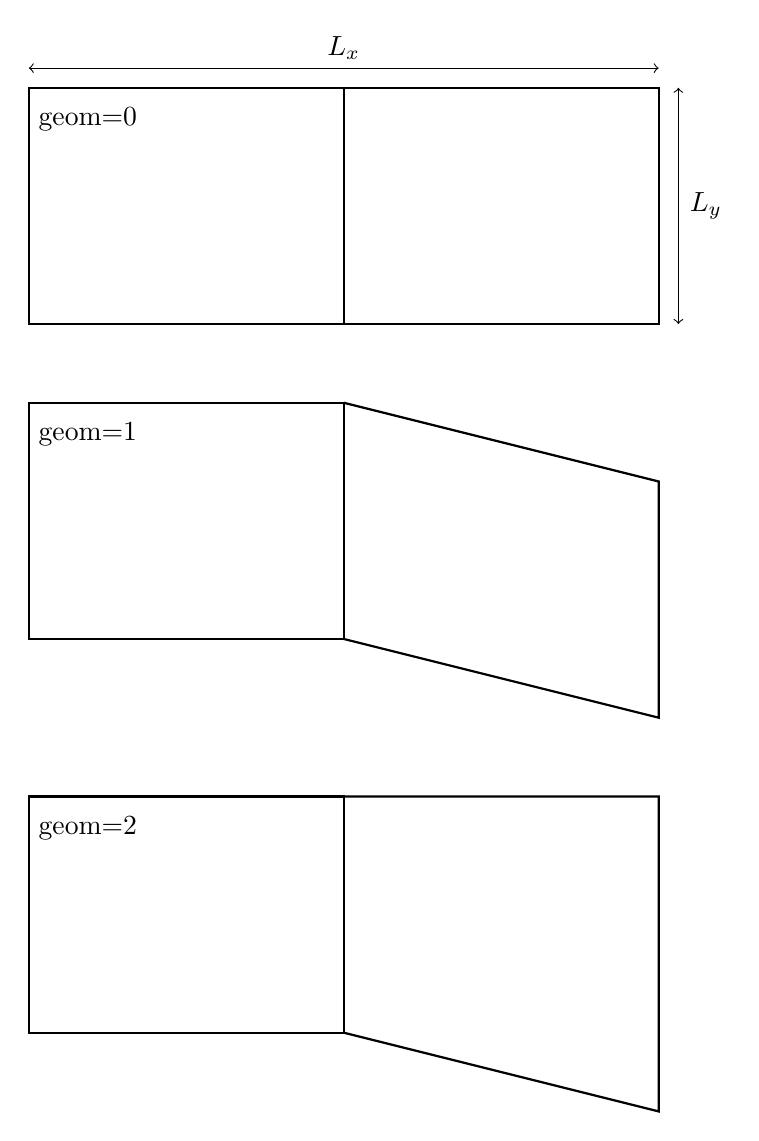
\begin{tikzpicture}
%\draw[step=1cm,gray,very thin] (0,0) grid (10,14); 
\draw[<->,thin] (1,13.25)--(9,13.25);
\node[] at (5,13.5) {$L_x$};
\draw[<->,thin] (9.25,10)--(9.25,13);
\node[] at (9.6,11.5) {$L_y$};
%.............................
\node[] at (1.75,12.6) {geom=$0$};
\draw[thick](1,10) rectangle (5,13); 
\draw[thick](5,10) rectangle (9,13); 
%.............................
\node[] at (1.75,8.6) {geom=$1$};
\draw[thick](1,6) rectangle (5,9);  
\draw[thick](5,6)--(9,5)--(9,8)--(5,9);  
%.............................
\node[] at (1.75,3.6) {geom=$2$};
\draw[thick](1,1) rectangle (5,4);  
\draw[thick](5,1)--(9,0)--(9,4)--(5,4);  
\end{tikzpicture}


\end{center}
and three different elements: ${\bm Q}_1\times P_0$, ${\bm Q}_2\times Q_1$, and ${\bm Q}_3\times Q_2$.

%.............................
\subsubsection{geom=0}

I find that the checkerboard mode is present for the unstable ${\bm Q}_1\times P_0$
element. However, for all three elements the velocity is zero, down to machine precision.
For the two continuous-pressure elements the pressure at the top is 0 and 6 at the 
bottom as expected.

\begin{center}
\includegraphics[width=5.4cm]{python_codes/fieldstone_42/results/geom0/press1}
\includegraphics[width=5.4cm]{python_codes/fieldstone_42/results/geom0/press2}
\includegraphics[width=5.4cm]{python_codes/fieldstone_42/results/geom0/press3}\\
\includegraphics[width=5.4cm]{python_codes/fieldstone_42/results/geom0/vel1}
\includegraphics[width=5.4cm]{python_codes/fieldstone_42/results/geom0/vel2}
\includegraphics[width=5.4cm]{python_codes/fieldstone_42/results/geom0/vel3}\\
{\captionfont From left to right: ${\bm Q}_1\times P_0$, ${\bm Q}_2\times Q_1$, 
and ${\bm Q}_3\times Q_2$.}
\end{center}


%.............................
\subsubsection{geom=1}

We find that the checkerboard mode is now absent and velocities are still zero
for all three elements. The pressure is hydrostatic and only depends on the $y$-coordinate.

\begin{center}
\includegraphics[width=5.1cm]{python_codes/fieldstone_42/results/geom1/press1}
\includegraphics[width=5.1cm]{python_codes/fieldstone_42/results/geom1/press2}
\includegraphics[width=5.1cm]{python_codes/fieldstone_42/results/geom1/press3}\\
\includegraphics[width=5.1cm]{python_codes/fieldstone_42/results/geom1/vel1}
\includegraphics[width=5.1cm]{python_codes/fieldstone_42/results/geom1/vel2}
\includegraphics[width=5.1cm]{python_codes/fieldstone_42/results/geom1/vel3}\\
{\captionfont From left to right: ${\bm Q}_1\times P_0$, ${\bm Q}_2\times Q_1$, 
and ${\bm Q}_3\times Q_2$.}
\end{center}

%.............................
\subsubsection{geom=2}

As in Fortin \& Fortin (1985) we find that the velocity field now showcases 2 ``convection
cells'' for the  ${\bm Q}_1\times P_0$ element (although they have different shapes than 
the ones in their publication) while the velocity remains zero for the other two elements. 

\begin{center}
\includegraphics[width=5.1cm]{python_codes/fieldstone_42/results/geom2/press1}
\includegraphics[width=5.1cm]{python_codes/fieldstone_42/results/geom2/press2}
\includegraphics[width=5.1cm]{python_codes/fieldstone_42/results/geom2/press3}\\
\includegraphics[width=5.1cm]{python_codes/fieldstone_42/results/geom2/vel1}
\includegraphics[width=5.1cm]{python_codes/fieldstone_42/results/geom2/vel2}
\includegraphics[width=5.1cm]{python_codes/fieldstone_42/results/geom2/vel3}\\
{\captionfont From left to right: ${\bm Q}_1\times P_0$, ${\bm Q}_2\times Q_1$, 
and ${\bm Q}_3\times Q_2$.}
\end{center}


On the following figure the root mean square velocity obtained with the 
${\bm Q}_1\times P_0$ element is shown as a function of 
the element size $h$. We find that it decreases quadratically with $h$. 
\begin{center}
\includegraphics[width=6cm]{python_codes/fieldstone_42/results/vrms.pdf}
\end{center}


 %%%%%%%%%%%%%%%%%%%%%%%%%%%%%%%%%%%%%%%%%%%%%%%%%

\newpage %%%%%%%%%%%%%%%%%%%%%%%%%%%%%%%%%%%%%%%%%%%%%%%%%%%%%%%%%%%%%%%%%%%%%%%%%%%%%%%%
\section*{
Stone 43: the rotating cone 
\label{f43}} 
\addcontentsline{toc}{section}{\protect\numberline{} 
Stone 43: the rotating cone 
}
This benchmark originates in \cite{dohu03}. It considers the advection of a product-cosine hill
in a prescribed velocity field. The initial temperature is:
\begin{equation}
T_0(x,y)=
\left\{
\begin{array}{cc}
\frac{1}{4}
\left(1+\cos \pi\frac{x-x_c}{\sigma}\right)
\left(1+\cos \pi\frac{y-y_c}{\sigma}\right)
& \text{if } (x-x_c)^2+(y-y_c)^2\leq \sigma^2 \\
0 & \text{otherwise}
\end{array}
\right.
\end{equation}
The boundary conditions are $T(x,y)=0$ on all four sides of the unit square domain. In what follows we set $x_c=y_c=1/6$ and $\sigma=0.2$.  The velocity field is analytically prescribed: $\vec\upnu=(-(y-y_c),+(x-x_c))$.

In what follows we test the time integration scheme by setting $\alpha_T=1$ (fully implicit formulation), $\alpha=0$ (fully explicit formulation) and $\alpha_T=1/2$ (Crank-Nicolson).  
The timestep is set to $\delta t=2\pi/200$. The density and heat capacity values are set to 1. 
We monitor the minimum and maximum value of the temperature field, as well as the total thermal energy $E_T$ in the system during the 200 time steps ($2\pi$ rotation of the cone):
\[
E_T=\int_\Omega \rho_0 c_p T dV = \int_\Omega T dV = |\Omega| \langle T \rangle 
\qquad
\text{where}
\qquad
\langle T \rangle = \frac{1}{|\Omega|} \int_\Omega T dV
\]
The time evolution of the temperature with the Crank-Nicolson algorithm is shown hereunder:
\begin{center}
a)\includegraphics[width=4.8cm]{python_codes/fieldstone_43/images/crni/velfield}
b)\includegraphics[width=4.8cm]{python_codes/fieldstone_43/images/crni/crnitemp0000}
c)\includegraphics[width=4.8cm]{python_codes/fieldstone_43/images/crni/crnitemp0050}\\
d)\includegraphics[width=4.8cm]{python_codes/fieldstone_43/images/crni/crnitemp0100}
e)\includegraphics[width=4.8cm]{python_codes/fieldstone_43/images/crni/crnitemp0050}
f)\includegraphics[width=4.8cm]{python_codes/fieldstone_43/images/crni/crnitemp0199}\\
{\small a) Velocity field and initial temperature; b,c,d,e,f) Temperature field at timesteps 0,50,100,150,199.} 
\end{center}
Turning now to the statistics, we plot $\min(T)$, $\max(T)$ and $E_T$ as a function of time:
\begin{center}
\includegraphics[width=5cm]{python_codes/fieldstone_43/images/Tmin.pdf}
\includegraphics[width=5cm]{python_codes/fieldstone_43/images/Tmax.pdf}
\includegraphics[width=5cm]{python_codes/fieldstone_43/images/ET.pdf}\\
{\small Time evolution of the min and max temperature and the total energy}
\end{center}
The conclusions are clear: the explicit method diverges quickly and is unusable. The fully implicit and Crank-Nicolson 
method yield similar energy conservation but the fully-implicit showcases a clear loss in maximum temperature as shown in the following figure:
\begin{center}
\includegraphics[width=15cm]{python_codes/fieldstone_43/images/temp}\\
{\small Temperature field after a full rotation with isocontours every 0.1 value.\\ Left: Fully-implicit; Right: Crank-Nicolson}
\end{center}

Finally we can run the experiment (still a $2\pi$ rotation) 
with three different time steps ($\delta t=2\pi/30,2\pi/60,2\pi/120$) 
and we recover very similar results to those presented in \cite{dohu03}:

\begin{center}
\includegraphics[height=8cm]{python_codes/fieldstone_43/images/dohu03}
\includegraphics[height=8cm]{python_codes/fieldstone_43/images/temps_30_60_120}\\
{\small From top to bottom: $\delta t=2\pi/120,2\pi/60,2\pi/30$ with Crank-Nicolson. Left panel is taken from donea \& Huerta \cite{dohu03}}
\end{center}

\begin{center}
\includegraphics[width=5cm]{python_codes/fieldstone_43/images/Tmin_CN.pdf}
\includegraphics[width=5cm]{python_codes/fieldstone_43/images/Tmax_CN.pdf}
\includegraphics[width=5cm]{python_codes/fieldstone_43/images/ET_CN.pdf}\\
{\small Time evolution of the min and max temperature and the total energy obtained with the Crank-Nicolson algorithm for 4 values of the timestep as indicated by the number between parenthesis.}
\end{center}

 %%%%%%%%%%%%%%%%%%%%%%%%%%%%%%%%%%%%%%%%%%%%%%%%%

\newpage %%%%%%%%%%%%%%%%%%%%%%%%%%%%%%%%%%%%%%%%%%%%%%%%%%%%%%%%%%%%%%%%%%%%%%%%%%%%%%%%
\section*{
Stone 44: the flat slab 
\label{f44}} 
\addcontentsline{toc}{section}{\protect\numberline{} 
Stone 44: the flat slab 
}

WORK in PROGRESS

I need a list of nodes on the boundary
I need a GCOORD.txt file with more decimals
I need an even lower resolution  grid
I need the scaling factors for rho,eta, ...


\includegraphics[width=14cm]{python_codes/fieldstone_44/grid_lowres1}\\
\includegraphics[width=7cm]{python_codes/fieldstone_44/grid_lowres2}
\includegraphics[width=7cm]{python_codes/fieldstone_44/grid_lowres3}\\
\includegraphics[width=7cm]{python_codes/fieldstone_44/grid_lowres4}
\includegraphics[width=7cm]{python_codes/fieldstone_44/grid_lowres5}


\begin{center}
\includegraphics[width=14cm]{python_codes/fieldstone_44/sifg19}\\
{\captionfont Taken from \cite{sifg19}}
\end{center}
 %%%%%%%%%%%%%%%%%%%%%%%%%%%%%%%%%%%%%%%%%%%%%%%%%


\newpage %%%%%%%%%%%%%%%%%%%%%%%%%%%%%%%%%%%%%%%%%%%%%%%%%%%%%%%%%%%%%%%%%%%%%%%%%%%%%%%%
\section*{
Stone 45: the corner flow
\label{f45}} 
\addcontentsline{toc}{section}{\protect\numberline{} 
Stone 45: the corner flow
}
\lstinputlisting[language=bash,basicstyle=\small]{python_codes/fieldstone_45/keywords}

\begin{center}
Code at \url{https://github.com/cedrict/fieldstone/tree/master/python_codes/fieldstone_45}
\end{center}

\par\noindent\rule{\textwidth}{0.4pt}

%%%%%%%%%%%%%%%%%%%%%%%%%%%%%%%%%%%%%%%%%%%%%%%%%%%%%%%%%%%%%%%%%%%%%%%%%%%%%%%%%%%%%%%%%%%%%%%%%%%%

The domain is a unit square. Only the pure advection equation is solved. 
The setup is identical to Experiment 1 of \stone 43. 
$P_1$ triangular elements are used. A Crank-Nicolson scheme is used for the time
discretisation. The mesh is based on splitting square cells. It is either  
perfectly regular or has some randomness added to it:

\begin{center}
\includegraphics[width=8.5cm]{python_codes/fieldstone_45/results/mesh_reg}
\includegraphics[width=8.5cm]{python_codes/fieldstone_45/results/mesh_rand}\\
{\captionfont Left: regular mesh of 30x30 cells; Right: same, with random noise added}
\end{center}

\begin{center}
\includegraphics[width=5.6cm]{python_codes/fieldstone_45/results/reg0000}
\includegraphics[width=5.6cm]{python_codes/fieldstone_45/results/reg0001}
\includegraphics[width=5.6cm]{python_codes/fieldstone_45/results/reg0002}\\
\includegraphics[width=5.6cm]{python_codes/fieldstone_45/results/reg0003}
\includegraphics[width=5.6cm]{python_codes/fieldstone_45/results/reg0004}
\includegraphics[width=5.6cm]{python_codes/fieldstone_45/results/reg0005}\\
{\captionfont Regular mesh. Temperature field after 0, $2\pi$, $4\pi$, $6\pi$, $8\pi$, $10\pi$ rotation}\\ 
\includegraphics[width=5.6cm]{python_codes/fieldstone_45/results/rand0000}
\includegraphics[width=5.6cm]{python_codes/fieldstone_45/results/rand0001}
\includegraphics[width=5.6cm]{python_codes/fieldstone_45/results/rand0002}\\
\includegraphics[width=5.6cm]{python_codes/fieldstone_45/results/rand0003}
\includegraphics[width=5.6cm]{python_codes/fieldstone_45/results/rand0004}
\includegraphics[width=5.6cm]{python_codes/fieldstone_45/results/rand0005}\\
{\captionfont Randomised mesh. Temperature field after 0, $2\pi$, $4\pi$, $6\pi$, $8\pi$, $10\pi$ rotation} 
\end{center}

\begin{center}
\includegraphics[width=10cm]{python_codes/fieldstone_45/results/T.pdf}\\
{\captionfont Minimum/maximum temperature as a function of time for both grids.} 
\end{center}
 %%%%%%%%%%%%%%%%%%%%%%%%%%%%%%%%%%%%%%%%%%%%%%%%%

\newpage %%%%%%%%%%%%%%%%%%%%%%%%%%%%%%%%%%%%%%%%%%%%%%%%%%%%%%%%%%%%%%%%%%%%%%%%%%%%%%%%
\section*{
Stone 46: MMS1 with Crouzeix-Raviart ($P_2^+\times P_{-1}$) elements  
\label{f46}} 
\addcontentsline{toc}{section}{\protect\numberline{} 
Stone 46: MMS1 with Crouzeix-Raviart ($P_2^+\times P_{-1}$) elements  
}

This stone showcases the Crouzeix-Raviart element (see Section~\ref{sec:crouzeix-raviart})
used to solve the analytical problem "Donea \& Huerta" (see Section~\ref{mms1}).

Out of convenience the pressure is set to zero at location $(x,y)=(1,1)$, so that the 
analytical solution is now $p(x,y)=x(1-x)$. 

\begin{center}
\includegraphics[width=5cm]{python_codes/fieldstone_46/grid}
\includegraphics[width=5cm]{python_codes/fieldstone_46/vel}
\includegraphics[width=5cm]{python_codes/fieldstone_46/press}\\
\includegraphics[width=5cm]{python_codes/fieldstone_46/exx}
\includegraphics[width=5cm]{python_codes/fieldstone_46/exy}
\end{center}

\begin{center}
\includegraphics[width=14cm]{python_codes/fieldstone_46/errors.pdf}
\end{center}

 %%%%%%%%%%%%%%%%%%%%%%%%%%%%%%%%%%%%%%%%%%%%%%%%%

\newpage %%%%%%%%%%%%%%%%%%%%%%%%%%%%%%%%%%%%%%%%%%%%%%%%%%%%%%%%%%%%%%%%%%%%%%%%%%%%%%%%
\section*{
Stone 47: MMS1 with MINI ($P_1^+\times P_1$) elements
\label{f47}} 
\addcontentsline{toc}{section}{\protect\numberline{} 
Stone 47: MMS1 with MINI ($P_1^+\times P_1$) elements
}
\lstinputlisting[language=bash,basicstyle=\small]{python_codes/fieldstone_47/keywords}

\begin{center}
Code at \url{https://github.com/cedrict/fieldstone/tree/master/python_codes/fieldstone_47}
\end{center}

\par\noindent\rule{\textwidth}{0.4pt}
%%%%%%%%%%%%%%%%%%%%%%%%%%%%%%%%%%%%%%%%%%%%%%%%%%%%%%%%%%%%%%%%%%%%%%%%%%%%%%%%%%%%%%%%%%%%

The domain is a unit cube. Free slip boundary conditions 
The grid is composed of triangles but for simplicity these 
are obtained by splitting rectangles in two, as shown hereunder:

\begin{center}
\includegraphics[width=8cm]{python_codes/fieldstone_47/images/minigrid}\\
Not shown are the nodes for the bubbles in the middle of each triangle. 
\end{center}

This stone showcases the MINI element (see Section~\ref{pair:mini})
used to solve the analytical problem "Donea \& Huerta" (see Section~\ref{mms1}).
Out of convenience the pressure is set to zero at location $(x,y)=(1,1)$, so that the 
analytical solution is now $p(x,y)=x(1-x)$. 

As an experiment I have run convergence tests for two cases: using nqel=3 
quadrature points and using nqel=6 quadrature points.
We find that the velocity and pressure errors converge depend on this crucial
parameter. 
For nqel=3 the velocity and pressure errors converge quadratically and linearly respectively
but for nqel=6 they converge as $h^2$ and $h^{1.5}$ respectively:

\begin{center}
\includegraphics[width=12cm]{python_codes/fieldstone_47/images/reg/errors}
\end{center}

It is worth noticing that although the element is stable, and the error converges
at a respectable rate, the pressure solution is not 'clean': as shown on the 
following figure, there is still some under/overshoot with respect to the analytical solution.

\begin{center}
\includegraphics[width=8cm]{python_codes/fieldstone_47/images/reg/pressure.pdf}
\includegraphics[width=6cm]{python_codes/fieldstone_47/images/rand/press}
\end{center}

Let us now explore the case where the nodes inside the domain are randomly perturbed, i.e. 
a random value  $(\delta_x,\delta_y)\in[-h_x/5,h_x/5]\times[-h_y/5,h_y/5]$ is added 
to their position (while preserving the position of the bubble as the barycenter of each triangle), 
as shown hereunder:

\begin{center}
\includegraphics[width=7cm]{python_codes/fieldstone_47/images/rand/grid}
\includegraphics[width=7cm]{python_codes/fieldstone_47/images/rand/areas}
\end{center}
 
Looking again at the convergence rates of the errors, we see that the velocity errors 
are virtually unchanged but we observe that the pressure errors no more align on a
single line and that the rates are only maintained on average. 

\begin{center}
\includegraphics[width=12cm]{python_codes/fieldstone_47/images/rand/errors}
\end{center}

 %%%%%%%%%%%%%%%%%%%%%%%%%%%%%%%%%%%%%%%%%%%%%%%%%

\newpage %%%%%%%%%%%%%%%%%%%%%%%%%%%%%%%%%%%%%%%%%%%%%%%%%%%%%%%%%%%%%%%%%%%%%%%%%%%%%%%%
\section*{
Stone 48: D\&H with $Q_1\times P_0$, $Q_2\times Q_1$, $Q_3\times Q_2$ and $Q_4\times Q_3$ elements
\label{f48}} 
\addcontentsline{toc}{section}{\protect\numberline{} 
Stone 48: D\&H with $Q_1\times P_0$, $Q_2\times Q_1$, $Q_3\times Q_2$ and $Q_4\times Q_3$ elements
}
In this experiment we consider 4 different finite elements. The idea behind this stone 
is to build a code which code(the FEM build and assembly) is common to all. 
The setup is the Donea \& HUerta benchmark (Section~\ref{mms1}), which has been modified so that 
the pressure is zero at the top right corner.

\begin{verbatim}

Q4xQ3                    Q3xQ2                  Q2xQ1                 Q1Q0

20===21===22===23===24  12====13====14====15  06======07=======08  02===============03
|                    |  |      |     |     |  |        |        |  |                 |
|                    |  |      |     |     |  |        |        |  |                 |
20===21===22===23===24  |      |     |     |  |        |        |  |                 |
|                    |  08====09====10====11  |        |        |  |                 |
|                    |  |      |     |     |  |        |        |  |                 |
20===21===22===23===24  |      |     |     |  03======04=======05  |                 |
|                    |  |      |     |     |  |        |        |  |                 |
|                    |  04====05====06====07  |        |        |  |                 |
20===21===22===23===24  |      |     |     |  |        |        |  |                 |
|                    |  |      |     |     |  |        |        |  |                 |
|                    |  |      |     |     |  |        |        |  |                 |
20===21===22===23===24  00====01====02====03  00======01=======02  00===============01 

12====13=====14=====15  06=======07=======08  02===============03  .=================.
|      |      |      |  |        |         |  |                 |  |                 |
|      |      |      |  |        |         |  |                 |  |                 |
|      |      |      |  |        |         |  |                 |  |                 |
08====09=====10=====11  |        |         |  |                 |  |                 |
|      |      |      |  |        |         |  |                 |  |                 |
|      |      |      |  03=======04=======05  |                 |  |       00        |
|      |      |      |  |        |         |  |                 |  |                 |
04====05=====06=====07  |        |         |  |                 |  |                 |
|      |      |      |  |        |         |  |                 |  |                 |
|      |      |      |  |        |         |  |                 |  |                 |
|      |      |      |  |        |         |  |                 |  |                 |
00====01=====02=====03  00=======01=======02  00===============01  .=================.

mV=25, mP=16            mV=16, mP=9           mV=9, mP=4           mV=4, mP=1      

\end{verbatim}

In the code the 'order' parameter can take values 1,2,3 and 4 which 
correspond to the polynomial order of the velocity approximation ($Q_1$, $Q_2$, $Q_3$ and $Q_4$).

When both nelx and nely values have been chosen, the total number of element 
for a regular 2D grid is simply:
\begin{lstlisting}
nel=nelx*nely
\end{lstlisting}

The number of nodes in each direction is then easily computed:
\begin{lstlisting}
nnx=order*nelx+1 
nny=order*nely+1 
\end{lstlisting}
and so is then the total number of velocity nodes:
\begin{lstlisting}
NV=nnx*nny
\end{lstlisting}

The total number of pressure nodes is as follows:
\begin{lstlisting}
if order==1:
   NP=nelx*nely
if order==2:
   NP=(nelx+1)*(nely+1)
if order==3:
   NP=(2*nelx+1)*(2*nely+1)
if order==4:
   NP=(3*nelx+1)*(3*nely+1)
\end{lstlisting}

Each velocity node has 2 dofs (ndofV=2) while pressure nodes have one dof (ndofP=1) so that 
the size of the blocks and the assembled FE matrix are given by:

\begin{lstlisting}
NfemV=NV*ndofV      
NfemP=NP*ndofP    
Nfem=NfemV+NfemP
\end{lstlisting}

For the linear element, 2 quadrature points per dimension are enough (nqperdim=2), 
while 3 are necessary for the quadratic element (nqperdim=3) and 4 are used  
for the cubic element (nqperdim=4), and 5 for the quartic element,
which can be conveniently implemented as follows:
\begin{lstlisting}
nqperdim=order+1
\end{lstlisting}
The quadrature points location and weight is document in Section~\ref{sec:quadrature}.

Because we wish to use a regular grid, the layout of the points for all three elements 
can be implemented easily:

\begin{lstlisting}
counter=0    
for j in range(0,nny):
    for i in range(0,nnx):
        xV[counter]=i*hx/order
        yV[counter]=j*hy/order
        counter+=1
\end{lstlisting}

The position of the pressure nodes follows a similar logic.

When it comes to the connectivity array, I first started by building it 
for each element as follows:

\begin{lstlisting}
if order==1:
   counter=0
   for j in range(0,nely):
       for i in range(0,nelx):
           iconV[0,counter]=(i)*1+0+(j)*1*nnx+nnx*0 
           iconV[1,counter]=(i)*1+1+(j)*1*nnx+nnx*0 
           iconV[2,counter]=(i)*1+0+(j)*1*nnx+nnx*1 
           iconV[3,counter]=(i)*1+1+(j)*1*nnx+nnx*1 
           counter += 1

if order==2:
   counter = 0
   for j in range(0,nely):
       for i in range(0,nelx):
           iconV[0,counter]=(i)*2+0+(j)*2*nnx+nnx*0 
           iconV[1,counter]=(i)*2+1+(j)*2*nnx+nnx*0 
           iconV[2,counter]=(i)*2+2+(j)*2*nnx+nnx*0 
           iconV[3,counter]=(i)*2+0+(j)*2*nnx+nnx*1 
           iconV[4,counter]=(i)*2+1+(j)*2*nnx+nnx*1 
           iconV[5,counter]=(i)*2+2+(j)*2*nnx+nnx*1 
           iconV[6,counter]=(i)*2+0+(j)*2*nnx+nnx*2 
           iconV[7,counter]=(i)*2+1+(j)*2*nnx+nnx*2
           iconV[8,counter]=(i)*2+2+(j)*2*nnx+nnx*2 
           counter += 1

if order==3:
   counter = 0
   for j in range(0,nely):
       for i in range(0,nelx):
           iconV[ 0,counter]=(i)*3+0+(j)*3*nnx+0*nnx 
           iconV[ 1,counter]=(i)*3+1+(j)*3*nnx+0*nnx 
           iconV[ 2,counter]=(i)*3+2+(j)*3*nnx+0*nnx 
           ...
           iconV[13,counter]=(i)*3+1+(j)*3*nnx+3*nnx 
           iconV[14,counter]=(i)*3+2+(j)*3*nnx+3*nnx 
           iconV[15,counter]=(i)*3+3+(j)*3*nnx+3*nnx 
           counter += 1
\end{lstlisting}
Having done so, it becomes quickly apparent that the connectivity array 
can be computed for all elements as follows:
\begin{lstlisting}
counter=0
for j in range(0,nely):
    for i in range(0,nelx):
        counter2=0
        for k in range(0,order+1):
            for l in range(0,order+1):
                iconV[counter2,counter]=i*order+l+j*order*nnx+nnx*k
                counter2+=1
        counter += 1
\end{lstlisting}
The same approach is taken to build the pressure connectivity array, 
although the $Q_1\times P_0$ element requires special attention since
the pressure is elemental and attributed to a single node inside the element. 

For the other elements I started from:

\begin{lstlisting}
if order==2:
   counter=0
   for j in range(0,nely):
       for i in range(0,nelx):
           iconP[0,counter]=(i)*1+0+(j)*1*(nelx+1)+(nelx+1)*0 
           iconP[1,counter]=(i)*1+1+(j)*1*(nelx+1)+(nelx+1)*0 
           iconP[2,counter]=(i)*1+0+(j)*1*(nelx+1)+(nelx+1)*1 
           iconP[3,counter]=(i)*1+1+(j)*1*(nelx+1)+(nelx+1)*1 
           counter += 1

if order==3:
   counter=0
   for j in range(0,nely):
       for i in range(0,nelx):
           iconP[0,counter]=(i)*2+0+(j)*2*(2*nelx+1)+(2*nelx+1)*0 
           iconP[1,counter]=(i)*2+1+(j)*2*(2*nelx+1)+(2*nelx+1)*0 
           iconP[2,counter]=(i)*2+2+(j)*2*(2*nelx+1)+(2*nelx+1)*0 
           iconP[3,counter]=(i)*2+0+(j)*2*(2*nelx+1)+(2*nelx+1)*1 
           iconP[4,counter]=(i)*2+1+(j)*2*(2*nelx+1)+(2*nelx+1)*1 
           iconP[5,counter]=(i)*2+2+(j)*2*(2*nelx+1)+(2*nelx+1)*1 
           iconP[6,counter]=(i)*2+0+(j)*2*(2*nelx+1)+(2*nelx+1)*2 
           iconP[7,counter]=(i)*2+1+(j)*2*(2*nelx+1)+(2*nelx+1)*2 
           iconP[8,counter]=(i)*2+2+(j)*2*(2*nelx+1)+(2*nelx+1)*2 
           counter += 1

if order==4:
   etc ...
\end{lstlisting}
and quickly arrived at the following compact form:
\begin{lstlisting}
if order>1:
   om1=order-1
   counter=0
   for j in range(0,nely):
       for i in range(0,nelx):
           counter2=0
           for k in range(0,order):
               for l in range(0,order):
                   iconP[counter2,counter]=i*om1+l+j*om1*(om1*nelx+1)+(om1*nelx+1)*k 
                   counter2+=1
           counter += 1
\end{lstlisting}

The core of the code is rather similar if not identical to other stones (i.e.
the loop over elements, the calculation of the elemental matrices, their assembly, 
and the solve).

What is here somewhat elegant is the projection of the pressure field onto the 
velocity grid nodes (mostly for plotting purposes). 
For each element I loop over each velocity node, and evaluate the 
pressure shape function at this location, compute the pressure with it 
and add it in the array q while keeping count of how many 
contributions there are in total per velocity node. 

\begin{lstlisting}
for iel in range(0,nel):
    for i in range(0,mV):
        NNNP[0:mP]=NNP(rVnodes[i],sVnodes[i],order)
        q[iconV[i,iel]]+=np.dot(p[iconP[0:mP,iel]],NNNP[0:mP])
        c[iconV[i,iel]]+=1.

q=q/c
\end{lstlisting}

Finally, since the vtu format does not support higher order elements, I 
here chose to only extract the corner values for each element, 
which translates as follows:
\begin{lstlisting}
vtufile.write("<DataArray type='Int32' Name='connectivity' Format='ascii'> \n")
if order==1:
   for iel in range (0,nel):
       vtufile.write("%d%d%d%d\n" %(iconV[0,iel],iconV[1,iel],iconV[3,iel],iconV[2,iel]))
if order==2:
   for iel in range (0,nel):
       vtufile.write("%d%d%d%d\n" %(iconV[0,iel],iconV[2,iel],iconV[8,iel],iconV[6,iel]))
if order==3:
   for iel in range (0,nel):
       vtufile.write("%d%d%d%d\n" %(iconV[0,iel],iconV[3,iel],iconV[15,iel],iconV[12,iel]))
if order==4:
   for iel in range (0,nel):
       vtufile.write("%d%d%d%d\n" %(iconV[0,iel],iconV[4,iel],iconV[24,iel],iconV[20,iel]))
vtufile.write("</DataArray>\n")
\end{lstlisting}


The following results are obtained by running one of the four scripts {\sl script\_errorsX} 
where X=1,2,3,4. The gnuplot script is to be found in the {\sl images} folder.

The stone implementes two ways of building the FE matrix. When the flag {\sl sparse} 
is false, the $\K$ and $\G$ matrices are built as full arrays, later assembled in a
larger full array, and then only converted to Compressed Sparse Row \index{CSR} before 
it is passed to the solver. When the flag is true, the global FE matrix 
is defined as a {\sl lil\_matrix} (a List of Lists) and it grows in size/memory
every time a new term is added to it. As shown on the following plot, it is about 
twice as slow compared to the first option, but it uses only a fraction of the memory
that the first one does. 

\begin{center}
\includegraphics[height=6.cm]{python_codes/fieldstone_48/images/FEMbuildtimes.pdf}
\end{center}

Also not very surprising: the cost of building the FE matrix increases with the order
of the used elements. A matrix corresponding to 100 $Q_1\times P_0$ elements can be 
built in about 1s, while it will take 7s when $Q_4 \times Q_3$ elements are used. 



%-------------------------------------------------
\subsection*{Results with $Q_1\times P_0$ element}


\begin{center}
\includegraphics[height=6.cm]{python_codes/fieldstone_48/images/q1q0/vel}
\includegraphics[height=6.cm]{python_codes/fieldstone_48/images/q1q0/p}\\
\includegraphics[height=4.cm]{python_codes/fieldstone_48/images/q1q0/pressure.pdf}
\includegraphics[height=4.cm]{python_codes/fieldstone_48/images/q1q0/errors1.pdf}
\end{center}

We see that we recover a second order convergence rate for velocity (as expected) 
but because of the checkerboard pattern the pressure convergence is simply random. 
The smoothed pressure $q$ shows virtually no checkerboard pattern, except on the boundaries.
This is a perfect example for the use of more accurate/clever smoothing procedure, see
Section~\ref{psmoothing}.


\subsection*{Results with $Q_2\times Q_1$ element}

We recover the cubic convergence for the velocity error and the quadratic convergence 
for the pressure:

\begin{center}
\includegraphics[width=8cm]{python_codes/fieldstone_48/images/errors2.pdf}
\end{center}

\subsection*{Results with $Q_3\times Q_2$ element}

The analytical solution is a second order polynomial, which means that the pressure 
shape functions can adequately represent the solution. We recover a fourth-order 
convergence for the velocity error and a superconvergent (fifth order) pressure error 
(but why is it 5th order ?).

\begin{center}
\includegraphics[width=8cm]{python_codes/fieldstone_48/images/errors3.pdf}
\end{center}

\subsection*{Results with $Q_4\times Q_3$ element}

Rather interestingly, now both velocity and pressure analytical solutions 
can be represented exactly by their respective polynomial spaces, so that 
the errors are at machine precision.

\begin{center}
\includegraphics[width=8cm]{python_codes/fieldstone_48/images/errors4.pdf}
\end{center}



 %%%%%%%%%%%%%%%%%%%%%%%%%%%%%%%%%%%%%%%%%%%%%%%%%

\newpage %%%%%%%%%%%%%%%%%%%%%%%%%%%%%%%%%%%%%%%%%%%%%%%%%%%%%%%%%%%%%%%%%%%%%%%%%%%%%%%%
\section*{
Stone 49: Consistent Boundary Flux method on D\&H benchmark with 4 elements 
\label{f49}} 
\addcontentsline{toc}{section}{\protect\numberline{} 
Stone 49: Consistent Boundary Flux method on D\&H benchmark with 4 elements 
}


%----------------------------------------------------
\subsection*{Looking at the four different elements}






%----------------------------------------------------
\subsection*{Looking at the influence of the mas matrix lumping}

 %%%%%%%%%%%%%%%%%%%%%%%%%%%%%%%%%%%%%%%%%%%%%%%%%

\newpage %%%%%%%%%%%%%%%%%%%%%%%%%%%%%%%%%%%%%%%%%%%%%%%%%%%%%%%%%%%%%%%%%%%%%%%%%%%%%%%%
\section*{
Stone 50: Lithosphere extension
\label{f50}} 
\addcontentsline{toc}{section}{\protect\numberline{} 
Stone 50: Lithosphere extension 
}


\includegraphics[width=16cm]{python_codes/fieldstone_50/solution.pdf}

 %%%%%%%%%%%%%%%%%%%%%%%%%%%%%%%%%%%%%%%%%%%%%%%%%

\newpage %%%%%%%%%%%%%%%%%%%%%%%%%%%%%%%%%%%%%%%%%%%%%%%%%%%%%%%%%%%%%%%%%%%%%%%%%%%%%%%%
\section*{
Stone 51: Triangular domain benchmark with MINI element
\label{f51}} 
\addcontentsline{toc}{section}{\protect\numberline{} 
Stone 51: Triangular domain benchmark with MINI element
}
{\sl This fieldstone was developed in collaboration with L. van de Wiel}. 


The following problem is studied in \cite{jolm17}.

The equation to solve are:
\begin{eqnarray}
-\vec{\nabla}p + \Delta \vec{\upnu} + Ra T \vec{e}_y &=& 0\\
\vec\nabla\cdot\vec\upnu &=& 0 \\
-\Delta T + \vec\upnu\cdot\nabla T &=& 0
\end{eqnarray}

The domain is chosen to be the right triangle
with vertices (0,0), (1,0), and (0,1). 
The boundary is considered to be solid walls (no-slip).
For the temperature, a sinusoidal heat source is enforced on the bottom
boundary with a Dirichlet condition ($T(x)=2(1-\cos (2\pi x))$), 
the left wall is set to a constant temperature
of zero, and the hypotenuse wall is perfectly insulated so that a Neumann 
boundary condition is appropriate.

\begin{center}
\includegraphics[width=6cm]{python_codes/fieldstone_51/minigrid5}
\end{center}




 %%%%%%%%%%%%%%%%%%%%%%%%%%%%%%%%%%%%%%%%%%%%%%%%%

\newpage %%%%%%%%%%%%%%%%%%%%%%%%%%%%%%%%%%%%%%%%%%%%%%%%%%%%%%%%%%%%%%%%%%%%%%%%%%%%%%%%
\section*{
Stone 52: Serendipity element in 2D 
\label{f52}} 
\addcontentsline{toc}{section}{\protect\numberline{} 
Stone 52: Serendipity element in 2D
}
In order to test the grid point and connectivity algorithms, 
we use this simple $4\times 3$ element mesh:

\begin{verbatim}

      Q_2 X Q1 (serendipity)                    Q_2 X Q_1 (regular)

15--47--16--48--17--49--18--50--19      54--55--56--57--58--59--60--61--62
 |       |       |       |       |       |   :   |   :   |   :   |   :   |
42      43      44      45      46      45..46..47..48..49..50..51..52..53
 |       |       |       |       |       |   :   |   :   |   :   |   :   |
10--38--11--39--12--40--13--41--14      36--37--38--39--40--41--42--43--44
 |       |       |       |       |       |   :   |   :   |   :   |   :   |
33      34      35      36      37      27..28..29..30..31..32..33..34..35
 |       |       |       |       |       |   :   |   :   |   :   |   :   |
05--29--06--30--07--31--08--32--09      18--19--20--21--22--23--24--25--26
 |       |       |       |       |       |   :   |   :   |   :   |   :   |
24      25      26      27      28      09..10..11..12..13..14..15..16..17
 |       |       |       |       |       |   :   |   :   |   :   |   :   |
00--20--01--21--02--22--03--23--04      00--01--02--03--04--05--06--07--08
\end{verbatim}

We see that the serendipity element-based mesh counts only 51 nodes, as
opposed to 63 for its counterpart.

Setting $nelx=nely$, we can look at the number of velocity nodes for each 
as a function of $nelx$, as shown hereunder:

\begin{center}
\includegraphics[width=6cm]{python_codes/fieldstone_52/NV.pdf}
\includegraphics[width=6cm]{python_codes/fieldstone_52/NV_ratio.pdf}
\end{center}
Looking at the ratio between both, we see that ultimately 
at high resolution, a mesh composed of serendipity elements 
will count 25\% less nodes than a mesh with Taylor-Hood elements.
Since there is not free lunch, what is the price paid in terms of accuracy when using 
the cheaper serendipity? 

The shape functions and their derivatives are in Section~\ref{sec:serendipity2D}.

Although the vtk format does not understand the $Q_2$ element in 2D or 3D, it surprisingly does
understand the serendipity element in 2D (type=23) and 3D (type=25).

\begin{center}
\includegraphics[width=8cm]{python_codes/fieldstone_52/errors.pdf}
\end{center}


 %%%%%%%%%%%%%%%%%%%%%%%%%%%%%%%%%%%%%%%%%%%%%%%%%

\newpage %%%%%%%%%%%%%%%%%%%%%%%%%%%%%%%%%%%%%%%%%%%%%%%%%%%%%%%%%%%%%%%%%%%%%%%%%%%%%%%%
\section*{
Stone 53: the sinking block benchmark 
\label{f53}} 
\addcontentsline{toc}{section}{\protect\numberline{} 
Stone 53: the sinking block benchmark 
}
\url{https://github.com/cedrict/fieldstone/tree/master/python_codes/fieldstone_53}

\vspace{1cm}

This simple benchmark provides challenging numerical experiments 
dealing with large viscosity variations within the simulation
domain. It appears in \cite{gery10} and consists of a bulk of fluid 1 ($\rho_1,\eta_1$)
in which a block of fluid 2 $(\rho_2,\eta_2)$ falls under its own
weight. The domain is a square of size $L_x=L_y=512$km and the
block is initially centred at point ($x=$256 km, $y=$ 384 km) with size
$128\times 128$ km:

\begin{center}
\includegraphics[height=5cm]{python_codes/fieldstone_53/images/setup}
\includegraphics[height=5cm]{python_codes/fieldstone_53/images/vel}\\
{\small Left: setup. Right: velocity field for $\rho_2=3208$, $\eta_1=10^{21}$
and $\eta_2=10^{22}$.}
\end{center}

The simulation is carried out on $32\times32$, $48\times48$ and $64\times 64$ grids. Free slip
boundary conditions are imposed on all sides of the domain. 
In all experiments the density of the surrounding fluid is $\rho_1=3200\text{kg}/\text{m}^3$.
The velocity $v_b$ of the falling block is measured in its centre (note that due to symmetry 
the horizontal component should be zero).

As explained in \cite{thie11}, following physical intuition, one expects 
the velocity $v_b$ of the block to (a) decrease when the viscosity
of the surrounding medium $\eta_1$ increases; (b) increase with the
density contrast $\rho_2-\rho_1$. 
The quantity $v_b \eta_1/(\rho_2-\rho_1)$ is therefore monitored and shown hereunder as a function of 
the viscosity ratio.


\begin{center}
\includegraphics[width=8cm]{python_codes/fieldstone_53/images/results.pdf}\\
{\small
Series of experiments have been conducted with $\rho_2=3208,3232,3328$, 
$\log_{10}(\eta_1)=20,21,22$ and $\log_{10}(\eta_2)=18,18.5,19,...22.5,23,23.5,24$, 
all with 3 mesh resolutions.}
 \end{center}

All experimental points line up on a single curve which further
indicates that the code can deal with gravity driven simulations in the presence
of large viscosity contrasts. These results have been succesfully compared with 
those obtained with ASPECT with the same setup.




 %%%%%%%%%%%%%%%%%%%%%%%%%%%%%%%%%%%%%%%%%%%%%%%%%












\newpage %%%%%%%%%%%%%%%%%%%%%%%%%%%%%%%%%%%%%%%%%%%%%%%%%%%%%%%%%%%%%%%%%%%%%%%%%%%%%%%%
\section{{\tt fieldstone}: Gravity: buried sphere} %%%%%%%%%%%%%%%%%%%%%%%%%%%%%%%%%%%%%%
Before you proceed further, please read :

\url{http://en.wikipedia.org/wiki/Gravity_anomaly}

\url{http://en.wikipedia.org/wiki/Gravimeter}

Let us consider a vertical domain $Lx \times Ly$ where $L_x=1000km$
and $Ly=500km$. This domain is discretised by means of a grid which counts $nnp= nnx \times nny$ nodes.
This grid then counts $nel=nelx \times nely = (nnx-1)\times(nny-1)$ cells.
The horizontal spacing between nodes is $hx$ and the vertical spacing is $hy$.

\begin{center}
\includegraphics[width=7cm]{/home/cedrict/Desktop/FIELDSTONE/fieldstone/python_codes/gravity_01/images/drawing}
\end{center}

Assume that this domain is filled with a rock type which 
mass density is given by $\rho_{medium}=3000kg/m^3$, 
and that there is a circular inclusion of another rock type  ($\rho_{sphere}=3200kg/m^3$) 
at location ($xsphere$, $ysphere$) of radius $rsphere$.
The density in the system is then given by 
\[
\rho(x,y) = 
\left\{
\begin{array}{l}
\rho_{sphere} \; {\rm  inside \; the\; circle} \\
\rho_{medium} \; {\rm outside \; the\; circle}
\end{array}
\right.
\]

Let us now assume that we place $nsurf$ gravimeters at the surface of the model. These are placed 
equidistantly between coordinates $x=0$ and coordinates $x=Lx$. We will use the arrays $xsurf$ and $ysurf$
to store the coordinates of these locations. 
The spacing between the gravimeters is $\delta_x=Lx/(nsurf-1)$.

At any given point $(x_i,y_i)$ in a 2D space, one can show that 
the gravity anomaly due to the presence of a 
circular inclusion can be computed as follows:
\begin{equation}
g(x_i,y_i)={2 \pi {\cal G} (\rho_{sphere}-\rho_0) R^2}\frac{y_i-y_{sphere}}{(x_i-x_{sphere})^2+(y_i-y_{sphere})^2}
\end{equation}
where $r_{sphere}$ is the radius of the inclusion, $(x_{sphere},y_{sphere})$ 
are the coordinates of the center of the inclusion, and
$\rho_0$ is a reference density.

However, the general formula to compute the gravity anomaly at a given point $(x_i,y_i)$ in space 
due to a density anomaly of any shape is given by:
\begin{equation}
g(x_i,y_i) = 2 {\cal G} \int\int_\Omega \frac{ \Delta \rho(x,y)  (y-y_i)}{(x-x_i)^2 + (y-y_i)^2  } dxdy
\end{equation}
where $\Omega$ is the area of the domain on which the integration is to be carried out. 
Furthermore the density anomaly can be written : $\Delta \rho (x,y)= \rho(x,y)-\rho_0$.
We can then carry out the integration for each cell and sum their contributions:
\begin{equation}
g(x_i,y_i) = 2 {\cal G} \sum_{ic=1}^{nel} \int\int_{\Omega_e} \frac{ (\rho(x,y) -\rho_0)  (y-y_i)}{(x-x_i)^2 + (y-y_i)^2  } dxdy
\end{equation}
where $\Omega_e$ is now the area of a single cell.
Finally, one can assume the density to be constant within each cell so that $\rho(x,y)\rightarrow \rho(ic)$
and $\int\int_{\Omega_e} dx dy \rightarrow hx \times hy$ and then 
\begin{equation}
g(x_i,y_i) = 2 {\cal G} \sum_{ic=1}^{nel} \frac{ (\rho(ic) -\rho_0)  (y(ic)-y_i)}{(x(ic)-x_i)^2 + (y(ic)-y_i)^2  } s_xs_y
\end{equation}

We will then use the array $gsurf$ to store the value of the gravity anomaly 
measured at each gravimeter at the surface. 

\begin{center}
\includegraphics[width=12cm]{/home/cedrict/Desktop/FIELDSTONE/fieldstone/python_codes/gravity_01/solution.pdf}
\end{center}


\paragraph{To go further}

\begin{itemize}
\item explore the effect of the size of the inclusion on the gravity profile.
\item explore the effect of the $\rho_0$ value.
\item explore the effect of the grid resolution.
\item measure the time that is required to compute the gravity. 
How does this time vary with nsurf ? how does it vary when the grid resolution is doubled ?
\item Assume now that $\rho_2<\rho_1$. What does the gravity profile look like ?
\item what happens when the gravimeters are no more at the surface of the Earth but in a satellite ?
\item if you feel brave, redo the whole exercise in 3D...
\end{itemize}

 %%%%%%%%%%%%%%%%%%%%%%%%%%%%%%%%%%%%%%%%%%%%%%%%%%%%

\newpage %%%%%%%%%%%%%%%%%%%%%%%%%%%%%%%%%%%%%%%%%%%%%%%%%%%%%%%%%%%%%%%%%%%%%%%%%%%%%%%%
\section{Problems, to do list and projects for students} %%%%%%%%%%%%%%%%%%%%%%%%%%%%%%%%

\begin{itemize}
\item Darcy flow. redo WAFLE (see http://cedricthieulot.net/wafle.html)
\item carry out critical Rayleigh experiments for various geometries/aspect ratios. Use Arie's notes. 
\item Newton solver
\item Corner flow 
\item elasticity with markers
\item Indentor/punch with stress b.c. ?
\item chunk grid
\item read in crust 1.0 in 2D on chunk
\item compute gravity based on tetrahedra
\item compare Q2 with Q2-serendipity
\item NS a la http://ww2.lacan.upc.edu/huerta/exercises/Incompressible/Incompressible\_Ex2.htm
\item produce example of mckenzie slab temperature
\item write about impose bc on el matrix
\item constraints
\item discontinuous galerkin
\item formatting of code style
\item navier-stokes ? (LUKAS) use dohu matlab code
\item nonlinear poiseuille
\item Finish nonlinear cavity case5.
\item write about mappings 
\item write about stream functions 
\item free surface 
\item zaleski disk advection
\item better yet simple matrix storage ?
\item write Scott about matching compressible2 setup with his paper
\item deal with large matrices. 
\item compositions, marker chain
\item free-slip bc on annulus and sphere . See for example p540 Gresho and Sani book.
\item non-linear rheologies (two layer brick spmw16, tosn15) 
\item Picard vs Newton
\item including phase changes (w. R. Myhill)
\item compute strainrate in middle of element or at quad point for punch?
\item GEO1442 code 
\item GEO1442 indenter setup in plane ?
\item in/out flow on sides for lith modelling
\item Fehlberg RK advection
\item redo puth17 2 layer experiment
\item create stone for layeredflow (see folder one up)
\item SIMPLE a la p667 \cite{john16} 
\item implement mms5 \ref{mms5}
\item implement/monitor div v
\item shape fct, trial fct, basis fct vs test fct doc
\item Delaunay triangulation, Voronoi, stripack
\end{itemize}

 %%%%%%%%%%%%%%%%%%%%%%%%%%%%%%%%%%%%%%%%%%%%%%%%%%%%%%%%%%%%%%%%%%%%%%%%

\appendix %========================================================================================

\newpage %%%%%%%%%%%%%%%%%%%%%%%%%%%%%%%%%%%%%%%%%%%%%%%%%%%%%%%%%%%%%%%%%%%%%%%%%%%%%%%%
%%%%%%%%%%%%%%%%%%%%%%%%%%%%%%%%%%%%%%%%%%%%%%%%%%%%%%%%%%%%%%%%%%%%%%%%%%%%%%%%%%%%%%%%%
\section{Three-dimensional applications} 
In the following table I list many papers which showcase high-resolution models of 
geodynamical processes (subduction, rifting, mantle flow, plume transport, ...).
Given the yearly output of our community and the long list of journal in which 
research can be disseminated, this list can not be exhaustive.

\noindent
{\small
\begin{tabular}{lll}
\hline
Ref.     & topic   & resolution \\
\hline
\hline
\cite{boht08b}& Effect of margin curvature on plate deformation in a 3D subduction zones        & \\
\cite{baiv10} & Small-scale sublithospheric convection in the Pacific                           & $448\times56\times64$ \\ 
\cite{stsf10} & Migration and morphology of subducted slabs in the upper mantle                 & $50\times50\times25$ \\
\cite{pyeg10} & Subduction scissor across the South Island of New Zealand                       & $17\times9\times9$ \\
\cite{mamb10} & Influence of a buoyant oceanic plateau on subduction zones                      & $80\times 40 \times80$ \\%(256,000 elts) \\
\cite{cafz11} & Subduction dynamics, origin of Andean orogeny and the Bolivian orocline         & $96\times96\times64$ \\%(590,000 elts) \\
\cite{ellw11} & Feedback between rifting and diapirism, ultrahigh-pressure rocks exhumation     & $100\times64\times20$ \\%\\($128,000$ elts) \\
\cite{alht11} & Numerical modeling of upper crustal extensional systems                         & $160\times160\times12$ \\%(307,200 elts) \\
\cite{alht12} & Rift interaction in brittle-ductile coupled systems                             & $160\times160\times23$ \\%(588,800 elts) \\
\cite{lehm12} & Kinematic interpretation of the 3D shapes of metamorphic core complexes         & $67\times67\times33$ \\%(150,000 elts)  \\
\cite{jabi12} & Role of rheology and slab shape on rapid mantle flow: the Alaska slab edge      & $960\times648\times160$ \\%(99,000,000 elts)$^1$ \\
\cite{cafa12} & Complex mantle flow around heterogeneous subducting oceanic plates              & $96\times96\times64$ \\%(590,000 elts) \\
\cite{brps12} & Oblique rifting and continental break-up                                        & $150\times50\times30$ \\%(225,000 elts) \\
\cite{bemm12} & Influence of mantle plume head on dynamics of a retreating subduction zone      & $80\times40\times80$\\% (256,000 elts \\
\cite{brau13} & Rift to break-up evolution of the Gulf of Aden                                  & $83\times83\times40$\\% (275,560 elts) \\
\cite{brps13} & Thermo-mechanical impact of plume arrival on continental break-up               & $100\times70\times20$\\% (140,000 elts) \\
\cite{care13} & Subduction and slab breakoff controls on Asian indentation tectonics            & $96\times96\times64$\\% (589,824 elts) \\
\cite{faca13} & Modeling of upper mantle deformation and SKS splitting calculations             & $96\times64\times96$ \\% (589,824 elts) \\
\cite{scmo13} & Backarc extension/shortening, slab induced toroidal/poloidal mantle flow        & $352\times 80 \times64$ \\%(1,802,240 elts) \\
\cite{magc13} & Sediment transports in the context of oblique subduction modelling              & $500\times 164\times 100$\\% (8,200,000 cells) \\
\cite{zhgt13} & Crustal growth at active continental margins                                    & $404\times164\times100$ \\%(6,625,600 cells) \\
\cite{lesh14} & Dynamics of India-Asia collision                                                & $257\times257\times 33$\\% (262,144 Q2P-1 elts) \\
\cite{whbb14} & Strain-partitioning in the Himalaya                                             & $256\times256\times40$ \\%(2,621,440 elts) \\
\cite{lixg13} & Collision of continental corner from 3-D numerical modeling                     & $500 \times 340 \times 164$ \\%(27,880,000 cells) \\
\cite{puge14} & Dependence of mid-ocean ridge morphology on spreading rate                      & $196\times196\times100$ \\%(3,841,600 cells)  \\
\cite{facc14} & Mid mantle seismic anisotropy around subduction zones                           & $197\times197\times53$ \\% (1,997,632 cells) \\
\cite{hebr14} & Oblique rifting of the Equatorial Atlantic                                      & $120\times80\times20$ \\%(192,000 elts) \\
\cite{mobm14} & Dynamics of continental accretion                                               & $256\times96\times96$ \\
\cite{rugb14} & Thrust wedges: infl. of decollement strength on transfer zones                  & $309\times85\times149$\\
\cite{buge14} & Asymmetric three-dimensional topography over mantle plumes                      & $500\times500\times217$ \\
\cite{thsh14} & modelled crustal systems undergoing orogeny and subjected to surface processes  & $96\times32\times14$\\
\cite{lige14b}& Thermo-mechanical modeling ontinental rifting and seafloor spreading            & $197\times197\times197$  \\ 
\cite{bemm15} & Geodynamics of oceanic plateau and plume head accretion                         & $256\times96\times96$ \\
\hline
\end{tabular}
}


 %%%%%%%%%%%%%%%%%%%%%%%%%%%%%%%
\newpage %%%%%%%%%%%%%%%%%%%%%%%%%%%%%%%%%%%%%%%%%%%%%%%%%%%%%%%%%%%%%%%%%%%%%%%%%%%%%%%%
\section{Codes in geodynamics \label{app:codes} }
In what follows I make a quick inventory of the main codes of computational geodynamics, 
for crust, lithosphere and/or mantle modelling.

in order to find all CIG-codes citations go to: https://geodynamics.org/cig/news/publications-refbase/

\begin{itemize}

%------------------------------------------------------------------------------
\item {\codefont ABAQUS} \index{general}{ABAQUS code}
%------------------------------------------------------------------------------

{\small
\noindent
\cite{brry01}
\cite{gedh02}
\cite{fumr03}
\cite{hapf06}
\cite{camg07}
\cite{kuhe09}
\cite{makh09}
\cite{camg10}
\cite{nalr12}
\cite{pevp15}
\cite{naam17}
\cite{naam18}
}

%------------------------------------------------------------------------------
\item {\codefont ANSYS} \index{general}{ANSYS code}
%------------------------------------------------------------------------------

\cite{nehe06}
\cite{guyr16}

%------------------------------------------------------------------------------
\item {\codefont ADELI} \index{general}{ADELI code}
%------------------------------------------------------------------------------

{\small
\noindent
1997: \cite{hajc97}\\
2001: \cite{chzh01}\\
2004: \cite{gocl04}\\
2006: \cite{vech06}\cite{golc06}\\
2008: \cite{boht08a}\cite{boht08b}\\
2012: \cite{gech12}\cite{gigh12}\\
2013: \cite{wahd13}\\
2014: \cite{cehg14}\\
2015: \cite{ceag15}\\
2018: \cite{cegm18}\cite{gehn18}
}

%------------------------------------------------------------------------------
\item {\codefont ASPECT} \index{general}{ASPECT code}
%------------------------------------------------------------------------------

This code is hosted by CIG at \url{https://geodynamics.org/cig/software/aspect/}. 
It is an open source community code based on the finite element library deal.II \cite{bahk07,arbc19}. 
It is massively parallel, relies on the p4est library for adaptive mesh refinement,
uses the Trilinos solver library \cite{hewi12}, and can deal with 2D and 3D geometries. 

\noindent
{\small
2012: \cite{krhb12}\\
2015: \cite{aupm15}\cite{tosn15}\\
2016: \cite{dahe16}\cite{gadb16}\cite{zhon16}\\
2017: \cite{hepb17}\cite{daef17}\cite{hedg17}\cite{robh17}\cite{robu17}\cite{aumh17}
      \cite{thie17}\cite{brsg17}\cite{onmz17}\cite{tasm17}\cite{zhli17}\\
2018: \cite{daga18}\cite{onzh18}\cite{gltf18}\cite{heps18}\cite{galh18}\cite{peka18}
      \cite{puth18}\cite{brst18b}\\
2019: \cite{baba19}\cite{stbl19}\cite{cocf19}\cite{liki19}\cite{galb19}\cite{dagg19}
      \cite{njas19}\cite{sepg19}\cite{ropu19}
}

%------------------------------------------------------------------------------
\item {\codefont BASIL/ELLE} \url{http://elle.ws/}
%------------------------------------------------------------------------------

{\small
\cite{bokj08}
\cite{llor19}
}

%------------------------------------------------------------------------------
\item {\codefont BEM} \index{general}{Boundary Element Method} \index{general}{BEM} 
%------------------------------------------------------------------------------

{\small
\cite{crsr83}
\cite{katl95}
\cite{moct07}
\cite{moct09}
\cite{moyb10}
\cite{qumm12}\cite{buqm12}
\cite{quhm13}
\cite{gert19}
}

%------------------------------------------------------------------------------
\item {\codefont CHIC}  \index{general}{CHIC code}
%------------------------------------------------------------------------------

\cite{norv15}

%------------------------------------------------------------------------------
\item {\codefont CitcomS} and {\codefont CitComCU} \index{general}{CitComS code}
%------------------------------------------------------------------------------

These codes are hosted by CIG at \url{https://geodynamics.org/cig/software/citcomcu/}
and \url{https://geodynamics.org/cig/software/citcoms/}.

{\small
\noindent
1995: \cite{moso95}\cite{mopa95}\\
1996: \cite{somo96}\cite{mogu96}\cite{zhgu96}\\
1997: \cite{mole97}\cite{bugm97}\cite{somo97}\\
1998: \cite{moso98}\cite{zhgm98}\cite{gumm98}\cite{resm98}\\
1999: \cite{mole99}\cite{bumo99}\cite{vazh99}\cite{lemo99}\cite{resm99}\\
2000: \cite{zhzm00}\cite{gumr00}\cite{lemm00}\cite{gumm00}\cite{somo00}\\
2001: \cite{bigu01}\cite{lemo01}\cite{zhon01}\\
2002: \cite{tagh02}\cite{somo02}\\
2003: \cite{vazh03}\cite{cogu03}\cite{bigu03}\cite{lemm03}\cite{lemo03}\cite{bigs03}\cite{vesh03}\\
2004: \cite{solo04}\cite{frmm04}\cite{lenm04}\cite{colm04}\cite{mczh04}\\
2005: \cite{bihi05}\cite{mczh05a}\cite{mczh05b}\cite{lemj05}\cite{zhon05}\\
2006: \cite{beck06}\cite{pibf06}\cite{tact06}\cite{besb06}\cite{coli06}\cite{frmm06}\cite{colm06}
      \cite{zhon06}\cite{keso06}\cite{rozh06}\cite{zhpy06}\\
2007: \cite{bihi07}\cite{zhzl07}\cite{magu07}\cite{bavi07}\cite{rimb07}\cite{mofm07}\cite{cobs07}
      \cite{qums07}\cite{huda07}\cite{rozh07}\\
2008: \cite{dihf08}\cite{gamc08}\cite{zhmt08}\cite{hole08}\cite{lejm08}\cite{lisg08}\cite{chzy08}
      \cite{beke08}\cite{beck08}\cite{slee08}\cite{lezh08}\cite{king08}\cite{ligu08}\cite{meco08}
      \cite{roni08}\cite{splg08}\cite{divf08}\cite{vavg08}\\
2009: \cite{lizh09}\cite{arhm09}\cite{zhzm09}\cite{anbi09}\cite{fobe09}\cite{bubi09}\cite{befa09}
      \cite{bavi09}\cite{lezh09}\cite{bogj09}\cite{zhon09}\cite{cohu09}\cite{coco09}\cite{keso09}
      \cite{maml09}\cite{nacl09}\cite{rolm09}\cite{splg09}\\
2010: \cite{bumb10}\cite{vabv10}\cite{baiv10}\cite{bubi10}\cite{zhzl10}\cite{bill10}\cite{cobe10}
      \cite{jabi10}\cite{zhst10}\cite{bofb10}\cite{hole10}\cite{hazs10}\cite{fabl10}\cite{dimg10}
      \cite{fabe10}\cite{ghbz10}\cite{lamg10}\cite{mcgr10}\cite{shml10}\cite{spgs10a,spgs10b}
      \cite{srzh10}\\
2011: \cite{befa11}\cite{lemj11}\cite{vaal11}\cite{legu11}\cite{list11}\cite{baiv11}\cite{bowg11}
      \cite{tree11}\cite{obbh11}\cite{bics11}\cite{zhxy11}\cite{digm11}\cite{orso11}\cite{mahg11}
      \cite{talz11}\cite{rapy11}\cite{scbb11}\cite{vasd11}\cite{vacg11}\cite{zhzh11}\\
2012: \cite{arbi12}\cite{jabi12}\cite{bija12}\cite{bova12}\cite{hucf12}\cite{zhym12}\cite{solo12}
      \cite{hibi12}\cite{jabk12}\cite{mapm12}\cite{solo12}\cite{trub12}\cite{cobu12}\cite{hats12}
      \cite{holr12}\cite{huco12}\cite{list12}\cite{mibe12}\cite{vacl12}\cite{naco12}\cite{roar12}
      \cite{roba12}\cite{shlm12}\cite{srzh12}\cite{wele12}\cite{zhzf12}\cite{zams12}\cite{mavf12}\\
2013: \cite{bacs13}\cite{bogs13a}\cite{bogs13b}\cite{jabr13}\cite{qula13}\cite{oldh13}
      \cite{arbi13}\cite{cost13}\cite{bugu13}\cite{flgm13}\cite{conr13}\cite{ghbh13}\cite{huyz13}
      \cite{kecl13}\cite{vagc13}\cite{mafv13}\cite{almb13}\\
2014: \cite{flgw14}\cite{budt14}\cite{kava14}\cite{arfw14}\cite{wavp14}\cite{seki14}
      \cite{agvg14}\cite{mabv14}\cite{zhu14}\\
2015: \cite{bacs15}\cite{bogf15}\cite{bomv15}\cite{sefw15}\cite{daso15}\cite{vami15}\cite{quxm15}
      \cite{wazh15}\cite{wavp15}\cite{waav15}\cite{hafg15}\cite{tarn15}\cite{legu15}\cite{tarn15}
      \cite{basn15}\cite{moba15}\cite{lizh15}\cite{welo15}\cite{wilm15}\cite{wahz15}\cite{hobb15}\\
2016: \cite{welm16}\cite{wele16}\cite{jada16}\cite{frbs16}\cite{robn16}\cite{boba16}\cite{mavm16}
      \cite{gulm16}\cite{kili16}\cite{mcnw16}\cite{wavp16}\cite{wahz16}\cite{wele16}\cite{yagz16}
      \cite{yagu16}\cite{jada16b}\cite{hulh16}\\
2017: \cite{aggv17}\cite{maav17}\cite{frbm17}\cite{haja17}\cite{majf17}\cite{ghts17}\cite{taac17}
      \cite{yagz17}\cite{lizh17}\cite{hobe17}\\
2018: \cite{hect18}\cite{king18}\cite{kavb18}\cite{wavp18}\cite{hulz18}\cite{lizo18}\cite{cimt18}
      \cite{trev18}\cite{wele18}\cite{yagz18}\cite{mazh18}\cite{biar18}\\
2019: \cite{mavb19}\cite{fube19}\cite{magn19}\cite{malg19}\cite{mazh19}\cite{boba19}\cite{lewh19}
      \cite{scvm19}\cite{almc19}\cite{rejv19}\cite{huzl19}\\
2020: \cite{weki20}\cite{braf20}\cite{vamg20}
}

%------------------------------------------------------------------------------
\item {\codefont COMSOL} \index{general}{COMSOL}
%------------------------------------------------------------------------------

\cite{ronb12}
\cite{cuwi14}
\cite{paml14b}

%------------------------------------------------------------------------------
\item {\codefont ConMan} \index{general}{ConMan code}
%------------------------------------------------------------------------------
This code is hosted by CIG at \url{https://geodynamics.org/cig/software/conman/}

{\small
\noindent
1990: \cite{kirh90}\cite{kiri00}\cite{gurn90}\cite{huha90}\cite{kiha90}\\
1991: \cite{kell91}\cite{lekb91}\\
1992: \cite{sqjs92}\cite{zhgu92}\\
1993: \cite{keki93}\cite{kief93}\cite{leka93}\cite{lekb93}\cite{zhgh93}\cite{zhgu93}\\
1994: \cite{itki94}\cite{fari94}\cite{gaha94}\cite{guto94}\cite{kiha94}\cite{leka94}\cite{leka94b}
      \cite{zhgu94b}\\
1995: \cite{kian95}\cite{leka95}\cite{lekb95}\cite{puhj95}\cite{pujh95}\cite{zhgu95b}\\
1996: \cite{laki96}\cite{leka96}\cite{mozg96}\cite{zhgm96}\\
1997: \cite{vaks97}\cite{keki97}\cite{kell97}\cite{mole97}\\
1998: \cite{kian98}\cite{itki98}\cite{vack08}\cite{kian98}\cite{lena98}\cite{mokm98}\\
1999: \cite{befo99}\cite{lemo99}\cite{como99}\cite{cori99}\cite{hagu99}\cite{roda99}\cite{sigh99}\\
2000: \cite{lemo00}\cite{conr00}\cite{elha00}\cite{lemo00}\\
2001: \cite{coha01}\cite{huke01}\\
2002: \cite{elvh02}\\
2003: \cite{fasa03}\cite{taki03}\cite{safa03}\cite{taki03}\\
2004: \cite{elhg04}\cite{shha04}\\
2005: \cite{kogk05}\cite{colt05}\cite{mish05}\cite{shha05}\cite{tagu05}\\
2006: \cite{nake06}\\
2007: \cite{nake07}\cite{dadh07}\cite{copb07}\cite{elki07}\cite{lohd07}\cite{nake07}\cite{reki07}\\
2008: \cite{hash08}\\
2009: \cite{faho09}\cite{heaa09}\cite{king09}\cite{leki09}\cite{wazh09}\\
2010: \cite{kilv10}\cite{cows10}\cite{hash10}\cite{leki10}\\
2011: \cite{hash11}\cite{leki11}\\
2014: \cite{kile14}\cite{leli14}\\
2015: \cite{kifr15}\cite{kilk15}\cite{lile15}
}

%------------------------------------------------------------------------------
\item {\codefont CONVRS} 
%------------------------------------------------------------------------------

{\small
\noindent
\cite{yoth12}
\cite{yosh13} 
} 

%------------------------------------------------------------------------------
\item {\codefont DOUAR} \index{general}{DOUAR code}
%------------------------------------------------------------------------------

{\small
\noindent
\cite{brtf08}\cite{thfb08}
\cite{yahb09}
\cite{brya10}\cite{lobh10}
\cite{mutg14}\cite{whbb14}
\cite{neew18}
\cite{koen19}
}

%------------------------------------------------------------------------------
\item Nameless code of Trompert and Hansen
%------------------------------------------------------------------------------

{\small
\cite{trha96}
\cite{trha98}\cite{trha98b}
\cite{goch04}
\cite{losh06}
\cite{loha08}\cite{stha08}
\cite{stfh10}
\cite{stlh13}
\cite{stha13}
\cite{stha14}
}

%------------------------------------------------------------------------------
\item MC3D \index{general}{MC3D code}
%------------------------------------------------------------------------------

\cite{stfl11}

%------------------------------------------------------------------------------
\item {\codefont DYNEARTHSOL} \index{general}{DYNEARTHSOL code}
%------------------------------------------------------------------------------

{\small
\noindent
\cite{chtl13}
\cite{jalr15}
\cite{lolc17}
}

%------------------------------------------------------------------------------
\item {\codefont GeoFEST} \index{general}{GeoFEST code}
%------------------------------------------------------------------------------
GeoFEST (Geophysical Finite Element Simulation Tool) is a two- and three-dimensional finite
element software package for the modeling of solid stress and strain in geophysical and 
other continuum domain applications.
The physics models supported include isotropic linear elasticity and both Newtonian and power-law
viscoelasticity, via implicit quasi-static time stepping. In addition to triangular, 
quadrilateral, tetrahedral and hexahedral continuum elements, GeoFEST supports split-node 
faulting, body forces, and surface tractions.


{\small
\noindent
\cite{paln08}
}

%------------------------------------------------------------------------------
\item {\codefont ELMER} \index{general}{ELMER code}
%------------------------------------------------------------------------------
Elmer is an open source multiphysical simulation software mainly developed by 
CSC - IT Center for Science (CSC). Elmer development was started 1995 in collaboration with 
Finnish Universities, research institutes and industry. Elmer includes physical models of 
fluid dynamics, structural mechanics, electromagnetics, heat transfer and acoustics, 
for example. These are described by partial differential equations which Elmer solves 
by the Finite Element Method (FEM). \url{https://www.csc.fi/web/elmer}

\cite{mals14}

%------------------------------------------------------------------------------
\item {\codefont LaCoDe} \index{general}{LaCoDe code} 
%------------------------------------------------------------------------------

{\small
\cite{demh19}
}

%------------------------------------------------------------------------------
\item {\codefont M-DOODS}, Duretz code
%------------------------------------------------------------------------------

{\small
\cite{yatd12}
\cite{yahb13}
\cite{yadm15}
\cite{chmd19}\cite{dual19}\cite{pedm19}
}

%------------------------------------------------------------------------------
\item {\codefont FENICS} \index{general}{FENICS code}
%------------------------------------------------------------------------------

\cite{alrk14}

%------------------------------------------------------------------------------
\item {\codefont GAIA} \index{general}{GAIA}
%------------------------------------------------------------------------------

{\small
\noindent
\cite{toyu11}
\cite{hutm13}
\cite{neum19}
}

%------------------------------------------------------------------------------
\item {\codefont GALE} \index{general}{GALE}
%------------------------------------------------------------------------------

This code is hosted by CIG at \url{https://geodynamics.org/cig/software/gale/}

{\small
\noindent
\cite{fabs08}
\cite{gotc08}
\cite{beve10}
\cite{cmwt10}
\cite{lehm12}\cite{liqi12}
\cite{arbi13}
}

%------------------------------------------------------------------------------
\item {\codefont (G)TECTON} \index{general}{GTECTON} \index{general}{TECTON}
%------------------------------------------------------------------------------

{\small
\noindent
1980: \cite{mera80}\\
1981: \cite{mera81}\\
1993: \cite{gowo93}\\
1995: \cite{gowo95}\\
1996: \cite{guez96}\cite{gisb96}\\
1999: \cite{gowo99}\cite{fugo99}\\
2001: \cite{bugw01}\cite{gome01}\\
2002: \cite{bugw02}\\
2005: \cite{gowo05}\cite{vanw05}\cite{vabl05}\cite{gowo05}\\
2006: \cite{degw06}\cite{libi06}\cite{scdm06}\\
2007: \cite{vabl07}\\
2008: \cite{degw08}\cite{degw08b}\\
2009: \cite{ladg09}\cite{plmg09}\\
2010: \cite{vago10}\cite{plmf10}\\
2011: \cite{bagw11}\cite{bagw11b}\\
2013: \cite{plab13}\cite{wagw13}\\
2014: \cite{vagw14}\\
2015: \cite{mags15}\cite{nigo15}\\
2016: \cite{gemg16}\cite{masg16}\\
2017: \cite{ozgw17}\\
2018: \cite{gofv18}\cite{nigw18}\cite{hefg18}
}

%------------------------------------------------------------------------------
\item {\codefont ELEFANT} \index{general}{ELEFANT code}
%------------------------------------------------------------------------------

{\small
\noindent
\cite{tosn15}
\cite{matv15}
\cite{busa16}
\cite{latb17}
\cite{thie17}
\cite{pltv18}
\cite{wohu19}
\cite{frtv19}
}

%------------------------------------------------------------------------------
\item {\codefont ELLIPSIS} \index{general}{ELLIPSIS code}
%------------------------------------------------------------------------------
Section 3 of \cite{qums07} presents the evolutionary path which lead to this code.

{\small
\noindent
2003: \cite{modm03}\cite{wibm03}\cite{mumc03}\cite{wemv03}\cite{onmo03}\\
2005: \cite{wiwg05}\cite{onml05}\cite{onmj05}\\
2006: \cite{onmm06} \\
2007: \cite{moql07}\cite{gewm07}\cite{dyrm07}\cite{onlm07}\\
2008: \cite{onlg08}\\
2009: \cite{onlj09}\\
2010: \cite{pyeg10}\\
2011: \cite{legu11}\\
2012: \cite{lega12}\\
2014: \cite{recf14}
}

%------------------------------------------------------------------------------
\item FANTOM \index{general}{FANTOM}
%------------------------------------------------------------------------------

{\small
\noindent
\cite{thie11}\cite{alht11}
\cite{alht12}
\cite{alhf13}
\cite{erhv14}\cite{thsh14}
\cite{erhv15}
\cite{sahf18}
\cite{erhv19}\cite{thhu19}
}

%------------------------------------------------------------------------------
\item FDCON \index{general}{FDCON}
%------------------------------------------------------------------------------

{\small
\noindent
\cite{enbs05}
\cite{crsg12}
\cite{fusc13}
\cite{fuks15}
}

%------------------------------------------------------------------------------
\item FLUIDITY \index{general}{FLUIDITY}
%------------------------------------------------------------------------------

{\small 
\noindent
\cite{dawk11}
\cite{krwd12}
\cite{gagd14}\cite{ledg14}
\cite{algg20}
}


%------------------------------------------------------------------------------
%\item IFISS 
%------------------------------------------------------------------------------
%\index{IFISS}
%Incompressible Flow Iterative Solution Solver is a
%MATLAB package that is a very useful tool for people interested in
%learning about solving PDE’s.
%IFISS includes built-in software for 2D versions of:
%the Poisson equation, the convection-diffusion equation, the Stokes equations
%and the Navier-Stokes equations.\\
%\url{https://personalpages.manchester.ac.uk/staff/david.silvester/ifiss/}

%------------------------------------------------------------------------------
\item {\codefont I2(3)E(L)VIS}  \index{general}{I2(3)(EL)VIS code}
%------------------------------------------------------------------------------

{\small
\noindent
2003: \cite{geyu03}\cite{geyu03b}\cite{geur03}\\
2004: \cite{geym04}\cite{geys04}\cite{gepm04}\cite{geur04}\\
2005: \cite{buge05}\cite{mage05}\cite{stge05}\\
2006: \cite{bbeg06}\cite{gest06}\cite{gogc06}\cite{gecy06}\\
2007: \cite{geyu07}\cite{gogc07}\cite{gebu07}\cite{gogg07}\cite{gowg07}\\
2008: \cite{scbe08}\cite{gecy08}\cite{uegs08}\cite{fagc08}\cite{zhgy09}\cite{buge08}
      \cite{cage08}\cite{migb08}\cite{nigc08}\cite{gepb08}\\
2009: \cite{gefc09}\cite{bubg09}\cite{ligt09}\cite{famg09}\cite{lige09}\\
2010: \cite{gerya2010}\cite{nigm10}\cite{bagc10}\cite{ligb10}\cite{sigb10}\\
2011: \cite{dugm11}\cite{dumg11}\cite{lixg11}\cite{gery11}\cite{geme11}\cite{blgg11}
      \cite{nigm11}\cite{gokg11}\cite{ligt11}\cite{pege11}\cite{zhgh11}\cite{gery11b}\\
2012: \cite{crsg12}\cite{dugk12}\cite{lixg12}\cite{fagm12}\cite{gohg12}\cite{uegb12}\cite{scgb12}
      \cite{sigb12}\cite{vogc12}\\
2013: \cite{lixg13}\cite{nabg13}\cite{magc13}\cite{vagd13a}\cite{vagd13b}\cite{zhgt13}\cite{dyge13}
      \cite{gemd13}\cite{mana13}\cite{chgz13}\cite{chgz13b}\cite{duge13}\cite{cavg13}\cite{ligw13}
      \cite{vocg13}\cite{gery13c}\cite{gery13}\cite{milp13}\cite{rugb13}\cite{scdg13}\\
2014: \cite{dugs14}\cite{puge14}\cite{voge14b}\cite{bagb14}\cite{lige14}\cite{stjm14}\cite{malg14}
      \cite{buge14}\cite{gosk14}\cite{vamd14}\cite{macg14}\cite{basc14}\cite{gobg14}\cite{gery14}
      \cite{gery14b}\cite{gita14}\cite{sigb14}\\
2015: \cite{uewg15}\cite{rula15}\cite{gesb15}\cite{rula15}\cite{kocb15}\cite{hevg15}\\
2016: \cite{kobc16}\cite{magc16}\cite{fige16}\cite{mauw16}\cite{duay16}\cite{mesj16}\cite{huwc16}
      \cite{staj16}\\
2017: \cite{mauw17}\cite{kocb17}\cite{vomc17}\cite{shwl17}\\
2018: \cite{zhlg18}\cite{masg18}\cite{gebu18}\cite{hegv18}\\
2019: \cite{kobg19}\cite{ligc19}\cite{sihf19}\cite{meag19}\cite{gubg19}\cite{vawg19}\\
2020: \cite{basg20}\cite{zhlg20}
}

%------------
\item I3MG

{\small
\noindent
\cite{facc14}
}

%------------------------------------------------------------------------------
\item LaMEM 
\index{general}{LaMEM code}
%------------------------------------------------------------------------------

{\small
\noindent
\cite{scbe08}
\cite{kamm10}
\cite{lemk11}
\cite{may12}
\cite{lesh14}\cite{cokm14}\cite{bakp14}\cite{feka14a}\cite{feka14b}
\cite{puka15}\cite{feka15}\cite{cofk15}
\cite{kapb16}\cite{coyc16}
\cite{pukp18}
\cite{eitp19}\cite{hooi19}
\cite{eitf20}\cite{spsk20}
}

%------------------------------------------------------------------------------
\item LAPEX2D,LAPEX3D  (LAgrangian Particle EXplicit, based on the prototype code PAROVOZ) 
\index{general}{LAPEX code}
%------------------------------------------------------------------------------

{\small
\noindent
\cite{sopg05}\cite{baso05}\cite{soba05}
\cite{bbeg06}\cite{basv06}\cite{sobk06}\cite{peso06}
\cite{peso08}\cite{baso08}\cite{scbe08}
\cite{sosk11}
}

%------------------------------------------------------------------------------
\item LITMOD2D/3D
%------------------------------------------------------------------------------

{\small 
\noindent
\cite{afrf07}
\cite{affr08}
\cite{fuac09}
\cite{fufa10}
\cite{jitf19}
}

%------------
%------------------------------------------------------------------------------
\item MARC
%------------------------------------------------------------------------------

{\small
\noindent
\cite{nesg97}
\cite{nesb99}
}


%------------------------------------------------------------------------------
\item {\codefont MILAMIN, MILAMIN\_VEP} 
\index{general}{MILAMIN}
\index{general}{MILAMIN\_VEP}
%------------------------------------------------------------------------------

MILAMIN is a finite element method implementation in native MATLAB that is capable of doing one million degrees of freedom per minute on a modern desktop computer. This includes pre-processing, solving, and post-processing. The MILAMIN strategies and package are applicable to a broad class of problems in Earth science. \url{http://milamin.org/}

{\small
\noindent
2008: \cite{daks08}\cite{scdk08}\\
2009: \cite{gogk09}\\
2010: \cite{krda10}\cite{kaus10}\cite{dekc10}\\
2011: \cite{yakm11}\\
2012: \cite{gebk12}\cite{rukb12}\cite{thka12}\\
2013: \cite{scpo13}\\
2014: \cite{jobk14}\\
2015: \cite{lukz15}\cite{gehm15}\cite{thkp15}\cite{musd15}\\
2016: \cite{jads16}\cite{maka16}\cite{cakp16}\\
2018: \cite{dusd18}\cite{jasc18}\cite{jadg18}\cite{comj18}\cite{jens18}\cite{rabw18}\cite{chsm18}\\
2019: \cite{anpa19}\cite{sifg19}\cite{baba19}\cite{sogh19}
}


%------------------------------------------------------------------------------
\item PARAVOZ/FLAMAR/FLAC 
\index{general}{FLAC} 
\index{general}{PARAVOZ} 
\index{general}{FLAMAR}
%------------------------------------------------------------------------------

{\small
\noindent
1989: \cite{cund89}\cite{hoor89}\\
1993: \cite{pocp93}\cite{zhhj93}\\
1994: \cite{wizh94}\\
1996: \cite{hach96}\cite{zhho96}\\
1998: \cite{gepd98}\\
2000: \cite{labp00}\\
2001: \cite{bujl01}\cite{bupo01}\\
2002: \cite{bast02}\cite{clbb02}\\
2003: \cite{hags03}\cite{gehd03}\cite{upke03}\\
2004: \cite{guhl04}\cite{gewi04}\cite{toba04}\cite{tibb04}\cite{clbm04}\cite{tobj04}\\
2005: \cite{bugu05}\\
2006: \cite{buwa06}\cite{lemm06}\\
2007: \cite{yaab07}\cite{buto07}\cite{chem07}\\
2008: \cite{yaba08}\cite{tibb08}\cite{buya08}\\
2009: \cite{gecm09}\cite{yahb09}\cite{bucl09}\cite{tigv09}\cite{yamb09}\\
2012: \cite{anwb12}\cite{gech12}\cite{gubc12}\cite{gerb12}\\
2013: \cite{wabd13}\cite{frbm13}\cite{tibb13}\\
2014: \cite{frba14}\cite{gagb14}\cite{bufa14}\cite{bufy14b}\\
2015: \cite{wulc15}\cite{gebw15}\cite{svlh15}\\
2016: \cite{marl16}\\
2018: \cite{gesr18}\\
2019: \cite{jala19}
}

%------------------------------------------------------------------------------
\item PINK3D
%------------------------------------------------------------------------------

{\small
\noindent
\cite{vosc15}
}


%------------------------------------------------------------------------------
\item PLASTI
%------------------------------------------------------------------------------

{\small
\noindent
\cite{fuwb06}
}

%------------------------------------------------------------------------------
\item pTatin3D: A nice succinct description of the code is given in Appendix B of \cite{lemh17}. 
\index{general}{pTatin3D}
%------------------------------------------------------------------------------

{\small
\noindent
2013: \cite{phil13}\\
2014: \cite{mabl14}\\
2015: \cite{mabl15}\\
2017: \cite{lemh17}\cite{magm17}\\
2018: \cite{jolp18}\\
2019: \cite{jolm19}
}

%------------------------------------------------------------------------------
\item PyLith \index{general}{PyLith}
%------------------------------------------------------------------------------
There are tons of papers with PyLith. 

{\small
\noindent
\cite{aakw13}
}

%------------------------------------------------------------------------------
\item PyGmod \index{general}{PyGmod}
%------------------------------------------------------------------------------

{\small
\noindent
\cite{crvs15}
}


%------------------------------------------------------------------------------
\item RHEA \index{general}{RHEA}
%------------------------------------------------------------------------------

{\small
\noindent
\cite{bugg08}
\cite{stgb10}
\cite{algs12}
\cite{busa13}
}

%------------------------------------------------------------------------------
\item SAMOVAR
%------------------------------------------------------------------------------

{\small
\noindent
\cite{egat10}
}

%------------------------------------------------------------------------------
\item {\codefont SEPRAN} 
\index{general}{SEPRAN code}
%------------------------------------------------------------------------------

SEPRAN \cite{sepr05} is a Fortran-based
multi-purpose Finite Element package developed by SEPRA engineering company in
cooperation with the department of applied mathematics of Delft Technical University
starting in the early 1980s. The package has been used for 25 yr in the education and
research program at Utrecht University and many students have used the package in
their work dealing with numerical modelling in geodynamics. SEPRAN is available for
a range of platforms including Linux/Unix and Microsoft Windows. It contains a mesh
generator with a flexible scripting interface for general 2-D and 3-D mesh configurations.

The package provides tools for a range of applications in science and engineering, in-
cluding second order elliptic, parabolic and hyperbolic equations, suitable for mechani-
cal problems dealing with linear elasticity and for flow problems for both incompressible
and compressible viscous media.

{\small
\noindent
1993: \cite{beky93}\cite{vavy93}\\
1994: \cite{vlvv94}\cite{vayv94}\\
1995: \cite{vayv95}\cite{vayu95}\\
1996: \cite{vayu96}\\
1997: \cite{vayu97}\cite{vank97}\\
1998: \cite{devv98}\\
1999: \cite{devv99}\\
2000: \cite{devv00b}\cite{vavv00}\\
2001: \cite{drvc01}\cite{vavv01}\\
2002: \cite{civv02}\cite{vavv02}\cite{vakp02}\cite{vavv02b}\cite{vaya02}\\
2003: \cite{vavd03}\cite{vabh03}\\
2004: \cite{vavv04}\cite{vavv04b}\cite{vavv04c}\cite{vayr04}\cite{vavv04d}\\
2005: \cite{vavv05}\cite{sepr05}\cite{vary05}\\
2006: \cite{liva06a}\cite{liva06b}\cite{abvk06}\\
2007: \cite{vant07}\cite{civv07}\cite{brva07a}\cite{brva07b}\cite{knvk07}\\
2008: \cite{plva08}\cite{brhv08}\cite{knva08}\cite{vava08}\\
2009: \cite{vavl09}\cite{vavv09}\\
2010: \cite{vahy10}\cite{syva10}\cite{devv10}\cite{vady10}\cite{vayb10}\\
2011: \cite{vahs11}\cite{java11}\cite{vayj11}\\
2012: \cite{besy12}\cite{beva12}\cite{chgv12}\\
2013: \cite{ancv13}\cite{cibi13}\\
2014: \cite{chsg14}\cite{mova14}\cite{chsv14}\\
2015: \cite{vasy15}\cite{cibi15}\\
2017: \cite{civj17}\cite{wewv17}\\
2018: \cite{spcv18}\cite{chss18}\\
2019: \cite{zhdv19}\cite{vayu19}\cite{casv19}\cite{vaws19}\cite{cibi19}
}



%------------------------------------------------------------------------------
\item {\codefont SHELLS} \index{general}{SHELLS code}
%------------------------------------------------------------------------------
It is a thin-shell program for modeling neotectonics of
regional or global lithosphere with faults

\cite{kobi95}

%------------------------------------------------------------------------------
\item {\codefont SISTER} \index{general}{SISTER code}
%------------------------------------------------------------------------------

{\small
\noindent
\cite{olbm16}
\cite{weib18}
}

%------------------------------------------------------------------------------
\item {\codefont SLIM3D} \index{general}{SLIM3D code}
%------------------------------------------------------------------------------

{\small
\noindent
\cite{poso08}
\cite{qusp10}
\cite{brps12}
\cite{brps13}
\cite{brau13}
\cite{brun14}
\cite{hebr14}
\cite{kobf14}
\cite{clbq15}
\cite{brcr17}
\cite{basq18}\cite{osss18}\cite{osss18b}
}

%------------------------------------------------------------------------------
\item {\codefont SLOMO} \index{general}{SLOMO code}
%------------------------------------------------------------------------------

{\small
\noindent
\cite{kaus05}
\cite{kasb08}
}

%------------------------------------------------------------------------------
\item {\codefont SNAC} \index{general}{SNAC code}
%------------------------------------------------------------------------------
SNAC (StGermaiN Analysis of Continua) is an updated Lagrangian explicit finite 
difference code for modeling a finitely deforming elasto-visco-plastic solid in 3D.
The code is hosted at \url{https://geodynamics.org/cig/software/snac/} .

{\small
\noindent
\cite{chlg08}
\cite{chgu08}
\cite{qula10}
\cite{chss11}
}

%------------------------------------------------------------------------------
\item {\codefont SPECFEM3D} 
\index{general}{SPECFEM3D code}
%------------------------------------------------------------------------------
SPECFEM3D Cartesian simulates acoustic (fluid), elastic (solid), coupled acoustic/elastic, 
poroelastic or seismic wave propagation in any type of conforming mesh of hexahedra 
(structured or not.) It can, for instance, model seismic waves propagating in sedimentary 
basins or any other regional geological model following earthquakes. It can also be used 
for non-destructive testing or for ocean acoustics. 

It is an open source code hosted by the CIG at 
\url{https://geodynamics.org/cig/software/specfem3d/}

{\small
\noindent
\cite{kott05}
}

%------------------------------------------------------------------------------
\item {\codefont MICROFEM}/{\codefont SOPALE} 
\index{general}{MICROFEM code}
\index{general}{SOPALE code}
%------------------------------------------------------------------------------
For an explanation of nested version of the numerical model, see appendix A of \cite{webe18}.

{\small
\noindent
1993: \cite{wibf93}\\
1994: \cite{wibe94}\cite{befh94}\cite{bequ94}\\
1995: \cite{full95}\cite{elfb95}\\
1996: \cite{bekh96}\cite{beeh96}\cite{wabe96}\\
1998: \cite{elbj98}\cite{jabf98}\cite{wabb98}\\
1999: \cite{will99a}\cite{will99b}\cite{elbp99}\cite{elbe99}\cite{beep99}\cite{pelj99}\\
2000: \cite{pybf00}\cite{bemh00}\cite{pfeb00}\\
2001: \cite{bejn01}\\
2002: \cite{hube02}\cite{pybf02}\\
2003: \cite{hube03}\cite{vamf03}\cite{wipo03}\cite{pymi03}\cite{bupf03}\cite{wiep03}\\
2004: \cite{bejn04}\cite{pycr04}\cite{pybe04}\cite{elsp04}\cite{geim04}\cite{jabm04}\\
2005: \cite{gebi05}\cite{hubb05}\\
2006: \cite{pysk06}\cite{selz06}\cite{pabs06}\cite{jabn06}\cite{benj06}\cite{cubj06}\cite{crnp06}\\
2007: \cite{hube07}\cite{cubh07}\cite{mohb07}\cite{sebp07}\cite{buto07b}\cite{jabn07}\cite{shpy07}\\
2008: \cite{sebp08}\cite{wabj08}\cite{wabj08b}\cite{gopy08}\cite{buhb08}\cite{hube08}\cite{cuhb08}\\
2009: \cite{kecw09}\cite{bejb09}\cite{bupb09}\cite{grba09}\cite{sihb09}\\
2010: \cite{albs10}\cite{albe10}\cite{grpy10}\cite{pygp10}\cite{albi10}\cite{jabw10}\cite{inbe10}
      \cite{inbe10b}\\
2011: \cite{cube11}\cite{bubj11}\cite{hube11}\cite{jabe11}\\
2012: \cite{grpy12}\cite{grpy12b}\cite{kogp12}\cite{grbe12}\cite{jahu12}\cite{albe12}\cite{grbi12}
      \cite{goib12}\cite{bein12}\\
2013: \cite{bubj13}\cite{chbe13}\cite{fihv13a}\cite{fihv13b}\cite{gobi13}\cite{grpy13}
      \cite{knak13}\cite{nipc13}\cite{krcu13}\\
2014: \cite{gogu14}\cite{jahm14}\cite{hube14}\cite{bubj14}\\
2015: \cite{albe15}\cite{bubj15}\cite{heps15}\cite{cudd15}\\
2016: \cite{licu16}\cite{albe16}\cite{kebb16}\\
2017: \cite{bube17}\cite{grbe17}\\
2018: \cite{webe18}\cite{webe18b}
}

%------------------------------------------------------------------------------
\item {\codefont STAG3D}/{\codefont STAGYY} \index{general}{STAG3D code} \index{general}{STAGYY code}
%------------------------------------------------------------------------------

{\small
\noindent
1994: \cite{tackley94}\\
1995: \cite{scta95}\\
1996: \cite{tack96}\cite{tack96b}\\
1998: \cite{most98}\cite{thta98}\\
2000: \cite{tack00}\cite{tack00b}\cite{tack00c}\cite{tack00d}\\
2001: \cite{tack01}\\
2002: \cite{falt02}\cite{tack02}\cite{taxi02}\\
2003: \cite{taxi03}\\
2004: \cite{xita04b}\cite{xita04}\cite{nata04}\cite{nata04b}\cite{nata04c}\cite{scmo04}\\
2005: \cite{grlt05}\cite{fasa05}\cite{nata05}\cite{nata05b}\cite{nabu05}\\
2006: \cite{mita06}\\
2007: \cite{grlt07}\cite{grlt07b}\cite{heta07}\cite{tanh07}\\
2008: \cite{deta08}\cite{hets08}\cite{heta08}\cite{sata08}\cite{nata08}\cite{tack08}\cite{vata08}\\
2009: \cite{deta09}\cite{natd09}\cite{keta09}\\
2010: \cite{detn10}\cite{nata10}\cite{moht10}\cite{sate10}\cite{natd10}\\
2011: \cite{rota11}\cite{gokg11}\cite{nata11}\\
2012: \cite{roct12}\cite{crtm12}\cite{cosr13}\cite{deyt12}\cite{dect12}\cite{arta12}\cite{natd12}
      \cite{ullc12}\\
2013: \cite{ruts13}\cite{taab13}\cite{nata13}\cite{mowe13}\\
2014: \cite{yadl14}\cite{crta14}\cite{roct14}\cite{cort14}\cite{becr14}\cite{lidt14}\cite{robg14}
      \cite{nata14}\\
2015: \cite{bect15}\cite{delt15}\cite{lidt15}\cite{nani15}\\
2016: \cite{sisc16}\cite{crta16}\\
2017: \cite{cogu17}\cite{pest17}\cite{bahh17}\cite{pact17}\\
2018: \cite{cosh18}\cite{bofc18}\cite{cold18}\cite{arcf18}\cite{cram18}\cite{crli18}\cite{lalt18}
      \cite{dert18}\\
2019: \cite{gult19}\cite{argc19}\cite{deli19}\cite{pact19}\cite{cohf19}\cite{crcm19}\cite{ulcw19}\\
2020: \cite{lalt20}\cite{gugb20}\cite{yabt20}
}

%------------------------------------------------------------------------------
\item {\codefont SUBMAR} \index{general}{SUBMAR code}
%------------------------------------------------------------------------------

{\small
\noindent
\cite{masr06}
\cite{masp07}
\cite{roms10}
}

%------------------------------------------------------------------------------
\item {\codefont SULEC} \index{general}{SULEC code}
%------------------------------------------------------------------------------

\url{http://www.geodynamics.no/buiter/sulec.html}

SULEC is a 2D/3D arbitrary Lagrangian Eulerian finite-element code developed by Susanne Buiter and Susan Ellis. 
It solves the equation for conservation of momentum for an incompressible fluid combined with 
the heat equation. Pressure is calculated as mean stress following an Uzawa iterative penalty 
formulation (Pelletier et al. (1989) \cite{pefc89}). 
Materials are tracked with tracers which are advected with a 2nd-order Runge-Kutta scheme. 
A true free surface is obtained by a slight vertical stretch of the Eulerian mesh to 
accommodate surface displacements and the effects of surface processes (Fullsack 1995 \cite{full95}). 
SULEC includes a stabilization term that suppresses numerical overshoot of isostatic restoring forces 
at interfaces with strong density contrasts (Kaus et al. (2010) \cite{kamm10}; 
Quinquis et al. (2011) \cite{qube11}). The mechanical and thermal equations are solved using 
the direct sparse solver PARDISO (Schenk and Gaertner (2004) \cite{scga04}).

{\small
\noindent
2011: \cite{qube11}\cite{ellw11}\\
2012: \cite{buit12}\cite{tebu12}\cite{crsg12}\cite{grel12}\\
2013: \cite{ghbu13}\\
2014: \cite{ghbu14}\cite{qubu14}\\
2015: \cite{nabu15}\\
2016: \cite{zwsn16}\\
2017: \cite{nabp17}\\
2018: \cite{tebu18}\\
2019: \cite{elgb19}
}

%------------------------------------------------------------------------------
\item {\codefont TERRA} \index{general}{TERRA code}
%------------------------------------------------------------------------------
The computational grid is based on a projection of the regular icosahedron onto a 
sphere and successive dyadic refinements \cite{bafr85}.  Concentric copies of such  
spherical layers of nodes build the domain in radial direction.
The first main improvement was being parallelised \cite{buba95}.
Particles were added in \cite{strb02}.

{\small
\noindent
1983: \cite{baum83}\\
1996: \cite{buri96}\\
1988: \cite{glat88}\\
1993: \cite{tasg93}\\
1994: \cite{tasg94}\\
1995: \cite{buba95}\\
1997: \cite{burb97}\cite{yang97}\\
1998: \cite{burl98}\\
1999: \cite{tabg99}\cite{ribr99}\\
2001: \cite{buda01}\cite{burm01}\cite{dabu01}\\
2002: \cite{burb02}\cite{strb02}\\
2005: \cite{phbu05}\\
2006: \cite{dabu06}\\
2007: \cite{phbu07}\\
2008: \cite{heib08}\cite{shlj08}\\
2009: \cite{phbs09}\cite{wodd09}\cite{gows09}\cite{iabu09}\cite{scbs09}\cite{scbs09b}
      \cite{scbr09}\cite{oebm09}\\
2010: \cite{yayh10}\\
2011: \cite{woda11}\cite{iahb11}\\
2012: \cite{dagd12}\cite{shbs12}\\
2013: \cite{dadb13}\cite{oflb13}\\
2014: \cite{butm14}\\
2015: \cite{amsb15}\cite{cobs15}\\
2016: \cite{vade16}\cite{necg16}\cite{pric16}\\
2017: \cite{woda17}\\
2018: \cite{ghbu18}\cite{cogb18}
}

%------------------------------------------------------------------------------
\item {\codefont TERRA-NEO} \index{general}{TERRA-NEO}
%------------------------------------------------------------------------------

\cite{wegg15}


%------------------------------------------------------------------------------
\item {\codefont TerraFERMA} \index{general}{TerraFERMA code}
%------------------------------------------------------------------------------
TerraFERMA is the Transparent Finite Element Rapid Model Assembler, a software system for the rapid and reproducible construction and exploration of coupled multi-physics models.

TerraFERMA leverages three advanced open-source libraries for scientific computation that provide high level problem description (FEniCS), composable solvers for coupled multi-physics problems (PETSc) and a science neutral options handling system (SPuD) that allows the hierarchical management of all model options.

TerraFERMA inherits most of its functionality from the underlying libraries but adds a layer of control and guidance for building reusable and reproducible applications.

\url{http://terraferma.github.io/}

{\small
\noindent
\cite{wisv14}
\cite{wisv17}
\cite{spmw16}
\cite{ceww17}
\cite{ceww19}
}

%------------------------------------------------------------------------------
\item {\codefont YACC} \index{general}{YACC code}
%------------------------------------------------------------------------------
This stands for 'Yet Another Convection Code'.

{\small
\noindent
\cite{sato12}
\cite{toyd13}
\cite{tosn15}
\cite{tomy16}
}

%------------------------------------------------------------------------------
\item {\codefont UNDERWORLD 1\&2} \index{general}{Underworld code}
%------------------------------------------------------------------------------
Section 3 of \cite{qums07} presents the evolutionary path which lead to this code.

{\small
\noindent
2006: \cite{stfs06}\cite{momu06}\\
2007: \cite{moql07}\cite{stfs07}\cite{qums07}\\
2008: \cite{lemm08}\cite{ozrs08}\cite{gotc08}\cite{stmt08}\cite{scsf11}\\
2010: \cite{casm10}\cite{mamb10}\cite{stsf10}\cite{stfc10}\cite{fasm10}\cite{cazf10}\\
2011: \cite{memm11}\cite{cafz11}\\
2012: \cite{cafa12}\\
2013: \cite{bemm12}\cite{scmo13}\cite{faca13}\cite{care13}\cite{coml13}\\
2014: \cite{famc14}\cite{shjm14}\\
2015: \cite{quxm15}\cite{bemm15}\cite{scsp15}\cite{shmj15}\cite{carr15}\\
2016: \cite{shmv16}\cite{onlw16}\cite{kicf16}\\
2017: \cite{bems17}\cite{kicf17}\cite{sche17}\cite{wakc17}\\
2018: \cite{memm18}\cite{yamz18}\cite{bemc18}\cite{mord18}\\
2019: \cite{samo19}\cite{yamg19}\cite{canc19}\cite{cakc19}\cite{sams19b}\cite{bore19}
}

%------------------------------------------------------------------------------
\item {\codefont VEMAN}
%------------------------------------------------------------------------------

{\small
\noindent
\cite{bepo10}
}

\end{itemize}
 %%%%%%%%%%%%%%%%%%%%%%%%%%
\newpage %%%%%%%%%%%%%%%%%%%%%%%%%%%%%%%%%%%%%%%%%%%%%%%%%%%%%%%%%%%%%%%%%%%%%%%%%%%%%%%%
\section{Matrix properties} \subsection{Symmetric matrices}

Any {\sl symmetric} matrix 
has only real eigenvalues,
is always diagonalizable,
and has orthogonal eigenvectors.
A symmetric $N\times N$ real matrix ${\bm M}$ is said to be
\begin{itemize}
\item {\bf positive definite} if $\vec x \cdot {\bm M} \cdot \vec x >0$ for every non-zero vector $\vec x$ of n real numbers. All the eigenvalues of a  Symmetric Positive Definite (SPD) matrix are positive.
 If A and B are positive definite, then so is A+B.
The matrix inverse of a positive definite matrix is also positive definite.
An SPD matrix has a unique Cholesky decomposition. In other words the matrix ${\bm M}$ 
is positive definite if and only if there exists a unique
lower triangular matrix ${\bm L}$, with real and strictly positive diagonal elements, 
such that ${\bm M} = {\bm L}{\bm L}^T$
(the product of a lower triangular matrix and its conjugate transpose).
This factorization is called the Cholesky decomposition of ${\bm M}$.
\index{Symmetric Positive Definite}

\item {\bf positive semi-definite} if $\vec x \cdot {\bm M} \cdot  \vec x \geq 0$
\item {\bf negative definite} if $\vec x \cdot {\bm M} \cdot \vec x < 0$
\item {\bf negative semi-definite} if $\vec x \cdot {\bm M} \cdot \vec x \leq 0$
\end{itemize}

The Stokes linear system
\[
\left( \begin{array}{cc}
\mathbb{K} & \mathbb{G}  \\ \mathbb{G}^T &  0
\end{array} \right) \cdot
\left( \begin{array}{c}  {\bm v} \\ {\bm p}  \end{array} \right) = 
\left( \begin{array}{c}  {\bm f} \\ {\bm g}  \end{array} \right) 
\]
is {\bf indefinite} (i.e. it has positive as well as negative eigenvalues).

A square matrix that is not invertible is called {\bf singular} or degenerate. A square matrix is singular if and only if its determinant is 0. Singular matrices are rare in the sense that if you pick a random square matrix, it will almost surely not be singular.

%--------------------------------
\subsection{Schur complement}

From wiki.
In linear algebra and the theory of matrices, the Schur complement of a matrix block (i.e., a submatrix within a larger matrix) is defined as follows.
Suppose ${\bm A}$, ${\bm B}$, ${\bm C}$, ${\bm D}$
are respectively $p\times p$, $p \times q$, $q \times p$ and $q \times q$ matrices, and $\mathbb{D}$ is invertible. Let
\[
{\bm M}=
\left( \begin{array}{cc}
{\bm A} & {\bm B}  \\ 
{\bm C} & {\bm D}
\end{array} \right) 
\]
so that ${\bm M}$ is a $(p+q)\times(p+q)$ matrix.
Then the Schur complement of the block ${\bm D}$ of the matrix ${\bm M}$ is the $p \times p$ matrix
\[
{\bm S}={\bm A}-{\bm B}\cdot {\bm D}^{-1}\cdot {\bm C}
\]
Application to solving linear equations: The Schur complement arises naturally 
in solving a system of linear equations such as
\begin{eqnarray}
{\bm A}\cdot\vec x+{\bm B}\cdot \vec y &=& \vec f \nonumber\\
{\bm C}\cdot\vec x+{\bm D}\cdot \vec y &=& \vec g \nonumber
\end{eqnarray}
where $\vec x$, $\vec f$ are $p$-dimensional vectors, $\vec y$, $\vec g$
are $q$-dimensional vectors,
and ${\bm A}$, ${\bm B}$, ${\bm C}$, ${\bm D}$ are as above.
Multiplying the bottom equation by ${\bm B}\cdot {\bm D}^{-1}$ 
and then subtracting from the top equation one obtains
\[
({\bm A}-{\bm B}\cdot {\bm D}^{-1}\cdot {\bm C})\cdot \vec x = \vec f - {\bm B}\cdot {\bm D}^{-1}\cdot \vec g
\]
Thus if one can invert ${\bm D}$ as well as the Schur complement of ${\bm D}$, one can solve for $\vec x$,
and then by using the equation $\bm C\cdot \vec x + \bm D \cdot \vec y = \vec g$ one can solve for $y$.
This reduces the problem of inverting a $(p+q) \times (p+q)$ matrix to that of inverting
a $p \times p$ matrix and a $q \times q$ matrix.
In practice one needs ${\bm D}$ to be well-conditioned in order for 
this algorithm to be numerically accurate.

Considering now the Stokes system: 
\[
\left( \begin{array}{cc}
\K & \G  \\ \G^T &  -\C
\end{array} \right) \cdot
\left( \begin{array}{c}  {\vec v} \\ {\vec p}  \end{array} \right) = 
\left( \begin{array}{c}  {\vec f} \\ {\vec g}  \end{array} \right) 
\]
Factorising for ${\vec p}$ we end up with a {\bf velocity-Schur complement}.
Solving for ${\vec p}$ in the second equation and inserting the expression
for ${\vec p}$ into the first equation we have
\[
\mathbb{S}_v \cdot {\vec v}  = {\vec f} 
\quad\quad
\text{with}
\quad\quad
\mathbb{S}_v=\K+ \G \cdot \C^{-1} \cdot \G^T
\]
Factorising for $\vec v$ we get a {\bf pressure-Schur complement}.
\[
\mathbb{S}_p \cdot {\vec p}  = \G^T \cdot \K^{-1}\cdot {\vec f}
\quad\quad
\text{with}
\quad\quad
\mathbb{S}_p = \G^T \cdot \K^{-1}\cdot \G + \C 
\]


 %%%%%%%%%%%%%%%%%%%%%%%%%%%%%%%%%%%%%%%%%%%%
\newpage %%%%%%%%%%%%%%%%%%%%%%%%%%%%%%%%%%%%%%%%%%%%%%%%%%%%%%%%%%%%%%%%%%%%%%%%%%%%%%%%
\section{Don’t be a hero - unless you have to} What follows was published online on July 17th, 2017 at 
\url{https://blogs.egu.eu/divisions/gd/2017/07/19/dont-be-a-hero-unless-you-have-to/}
It was written by me and edited by Iris van Zelst, at the time PhD student at ETH Z\"urich.

\vspace{3mm}

In December 2013, I was invited to give a talk about the \aspect{} code [1] 
at the American Geological Union conference in San Francisco. Right 
after my talk, Prof. Louis Moresi took the stage and gave a talk entitled: 
{\it Underworld: What we set out to do, How far did we get, What did we Learn?}

The abstract went as follows:

"Underworld was conceived as a tool for modelling 3D lithospheric deformation coupled with the underlying / surrounding mantle flow. The challenges involved were to find a method capable of representing the complicated, non-linear, history dependent rheology of the near surface as well as being able to model mantle convection, and, simultaneously, to be able to solve the numerical system efficiently. […] The elegance of the method is that it can be completely described in a couple of sentences. However, there are some limitations: it is not obvious how to retain this elegance for unstructured or adaptive meshes, arbitrary element types are not sufficiently well integrated by the simple quadrature approach, and swarms of particles representing volumes are usually an inefficient representation of surfaces."

Aside from the standard numerical modelling jargon, Louis used a term during his talk which I thought at the time had a nice ring to it: hero codes. In short, I believe he meant the codes written essentially by one or two people who at some point in time spent great effort into writing a code (usually choosing a range of applications, a geometry, a number of dimensions, a particular numerical method to solve the relevant PDEs(1), and a tracking method for the various fields of interest).

In the long list of Hero codes, one could cite (in alphabetical order) CITCOM [1], \douar [8], \fantom [2], IELVIS [5], LaMEM [3], pTatin [4], SLIM3D [10], \sopale [7], StaggYY [6], \sulec [11], Underworld [9], and I apologise to all other heroes out there whom I may have overlooked. And who does not want to be a hero? The Spiderman of geodynamics, the Superwoman of modelling?

Louis' talk echoed my thoughts on two key choices we (computational geodynamicists) are facing: Hero or not, and if yes, what type?

\vspace{3mm}

{\bf Hero or not?}

\vspace{3mm}

Speaking from experience, it is an intense source of satisfaction when peer-reviewed published results are obtained with the very code one has painstakingly put together over months, if not years. But is it worth it?

On the one hand, writing one own’s code is a source of deep learning, a way to ensure that one understands the tool and knows its limitations, and a way to ensure that the code has the appropriate combination of features which are necessary to answer the research question at hand. On the other hand, it is akin to a journey; a rather long term commitment; a sometimes frustrating endeavour, with no guarantee of success. Let us not deny it – many a student has started with one code only to switch to plan B sooner or later. Ultimately, this yiels a satisfactory tool with often little to no perennial survival over the 5 year mark, a scarce if at all existent documentation, and almost always not compliant with the growing trend of long term repeatability. Furthermore, the resulting code will probably bear the marks of its not-all-knowing creator in its DNA and is likely not to be optimal nor efficient by modern computational standards.

This brings me to the second choice: elegance \& modularity or taylored code \& raw performance? Should one develop a code in a very broad framework using as much external libraries as possible or is there still space for true heroism?

It is my opinion that the answer to this question is: both. The current form of heroism no more lies in writing one’s own FEM(2)/FDM(3) packages, meshers, or solvers from scratch, but in cleverly taking advantage of state-of-the-art packages such as for example p4est [15] for Adaptive Mesh Refinement, PetSc [13] or Trilinos [14] for solvers, Saint Germain [17] for particle tracking, deal.ii [12] or Fenics [16] for FEM, and sharing their codes through platforms such as svn, bitbucket or github.

In reality, the many different ways of approaching the development or usage of a (new) code is linked to the diversity of individual projects, but ultimately anyone who dares to touch a code (let alone write one) is a hero in his/her own right: although (super-)heroes can be awesome on their own, they often complete each other, team up and join forces for maximum efficiency. Let us all be heroes, then, and join efforts to serve Science to the best of our abilities.

\vspace{3mm}

\noindent Abbreviations

(1) PDE: Partial Differential Equation 

(2) FEM: Finite Element Method 

(3) FDM: Finite Difference Method

\noindent References

[1] Zhong \etal, JGR 105, 2000; 

[2] Thieulot, PEPI 188, 2011; 

[3] Kaus \etal, NIC Symposium proceedings, 2016; 

[4] May \etal, CMAME 290, 2015 

[5] Gerya and Yuen, PEPI 163, 2007 

[6] Tackley, PEPI 171, 2008 

[7] Fullsack, GJI 120, 1995 

[8] Braun \etal, PEPI 171, 2008 

[9] http://www.underworldcode.org/ 

[10] Popov and Sobolev, PEPI 171, 2008 

[11] http://www.geodynamics.no/buiter/sulec.html 

[12] Bangerth \etal, J. Numer. Math., 2016; http://www.dealii.org/ 

[13] http://www.mcs.anl.gov/petsc/ 

[14] https://trilinos.org/ 

[15] Burstedde \etal, SIAM journal on Scientific Computing, 2011; http://www.p4est.org/ 

[16] https://fenicsproject.org/ 

[17] Quenette \etal, Proceedings 19th IEEE, 2007





 %%%%%%%%%%%%%%%%%%%%%%%%%%%%%
\newpage %%%%%%%%%%%%%%%%%%%%%%%%%%%%%%%%%%%%%%%%%%%%%%%%%%%%%%%%%%%%%%%%%%%%%%%%%%%%%%%%
\section{A FANTOM, an ELEFANT and a GHOST} While a post-doctoral researcher at Bergen University I developed the FANTOM code. Here is what other people and I have published with it:

\begin{itemize}

\item {\it FANTOM : two- and three-dimensional numerical modelling of creeping flows for the solution of geological problems}, 
C. Thieulot, Physics of the Earth and Planetary Interiors, 188, 2011.

\begin{center}
\includegraphics[width=8cm]{images/mycodes/thie11_img}
\end{center}


\item {\it Three-dimensional numerical modeling of upper crustal extensional systems}, 
V. Allken, R.S. Huismans and C. Thieulot, JGR 116, 2011. \url{https://doi:10.1029/2011JB008319} 

\begin{center}
\includegraphics[height=3cm]{images/mycodes/alht11_img}
\end{center}


\item {\it Factors controlling the mode of rift interaction in brittle-ductile coupled systems: A 3D numerical study}, 
V. Allken, R.S. Huismans and C. Thieulot, Geochem. Geophys. Geosyst. 13(5), 2012.
\url{https://doi:10.1029/2012GC004077}

\begin{center}
\includegraphics[height=3cm]{images/mycodes/alht12_img}
\end{center}


\item {\it 3D numerical modelling of graben interaction and linkage: a case study of the Canyonlands grabens, Utah}, 
V. Allken, R.S. Huismans, Haakon Fossen and C. Thieulot, Basin Research, 25, 1-14, 2013.
\url{https://doi: 10.1111/bre.12010}

\begin{center}
\includegraphics[height=3cm]{images/mycodes/alhf13_img}
\end{center}


\item {\it Three-dimensional numerical simulations of crustal systems undergoing orogeny and subjected to surface processes}, 
C. Thieulot, P. Steer and R.S. Huismans, Geochem. Geophys. Geosyst., 15, 2014. doi:10.1002/2014GC005490

\item {\it Extensional inheritance and surface processes as controlling factors of mountain belt structure}, 
Z. Erd\"os, R.S. Huismans, P. van der Beek, and C. Thieulot, J. Geophys. Res. Solid Earth, 119, 2014. doi:10.1002/2014JB011408

\item {\it First-order control of syntectonic sedimentation on crustal-scale structure of mountain belts}, 
Z. Erd\"os, R.S. Huismans, P. van der Beek, J. Geophys. Res. Solid Earth, 120, 5362-5377, 2015. doi:10.1002/2014JB011785

\item {\it Control of increased sedimentation on orogenic fold-and-thrust belt structure - insights into the evolution of the Western Alps}, 
Z. Erd\"os, R.S. Huismans and P. van der Beek, Solid Earth, 10, 391-404, 2019.
\url{https://doi.org/10.5194/se-10-391-2019}

\begin{center}
\includegraphics[height=3cm]{images/mycodes/erhv19_img}
\end{center}

\item {\it Mountain building or backarc extension in ocean-continent subduction systems - a function of
backarc lithospheric strength and absolute plate velocities}, 
S.G. Wolf and R.S. Huismans, JGR, 2019. \url{https://doi.org/10.1029/2018JB017171}

\begin{center}
\includegraphics[height=3cm]{images/mycodes/wohu19_img}
\end{center}


\end{itemize}

Upon my arrival at Utrecht University in 2012 I started working an a more flexible code, called ELEFANT, which has since very much 
diverged from FANTOM.

\begin{itemize}
\item {\it The effect of obliquity on temperature in subduction zones: insights from 3-D numerical modeling}, 
A. Plunder, C. Thieulot and D.J.J. van Hinsbergen, Solid Earth 9, 759-776, 2018. \url{https://doi.org/10.5194/se-9-759-2018}

\begin{center}
\includegraphics[height=3.5cm]{images/mycodes/pltv18_img}
\end{center}


\item {\it Analytical solution for viscous incompressible Stokes flow in a spherical shell}, 
C. Thieulot, Solid Earth 8, 1181-1191, 2017. \url{https://doi.org/10.5194/se-8-1181-2017}

\begin{center}
\includegraphics[height=3cm]{images/mycodes/thie17}
\end{center}



\item  {\it Lithosphere erosion and continental breakup: interaction of extension, plume upwelling and melting}, 
A. Lavecchia, C. Thieulot, F. Beekman, S. Cloetingh and S. Clark, E.P.S.L. 467, p89-98, 2017.

\begin{center}
\includegraphics[height=3cm]{images/mycodes/latv17_img}
\end{center}


\item {\it Benchmarking numerical models of brittle thrust wedges}, 
Susanne J.H. Buiter, Guido Schreurs, Markus Albertz, Taras V. Gerya, Boris Kaus,
Walter Landry, Laetitia le Pourhiet, Yury Mishin, David L. Egholm, Michele Cooke,
Bertrand Maillot, Cedric Thieulot, Tony Crook, Dave May, Pauline Souloumiac, Christopher Beaumont
Journal of Structural Geology 92, p140-177, 2016. \url{https://doi:10.1016/j.jsg.2016.03.003}

\begin{center}
\includegraphics[height=1.8cm]{images/mycodes/busa16_img}
\end{center}


\item {\it A community benchmark for viscoplastic thermal convection in a 2-D square box}, 
N. Tosi, C. Stein, L. Noack, C. Huettig, P. Maierova, H. Samuel, D.R. Davies, C.R. Wilson, S.C. Kramer, C. Thieulot, A. Glerum, M. Fraters, W. Spakman, A. Rozel, P.J. Tackley, Geochem. Geophys. Geosyst. 16, doi:10.1002/2015GC005807, 2015.

\begin{center}
\includegraphics[height=3cm]{images/mycodes/tosn15_img}
\end{center}


\item {\it Dynamics of intraoceanic subduction initiation: 1. Oceanic detachment fault inversion and the formation of supra-subduction zone ophiolites}, M. Maffione, C. Thieulot, D.J.J. van Hinsbergen, A. Morris, O. Pluemper and W. Spakman, Geochem. Geophys. Geosyst. 16, p1753-1770, 2015.

\begin{center}
\includegraphics[height=1.8cm]{images/mycodes/matv15_img}
\end{center}

\item {\it The Geodynamic World Builder: a solution for complex initial conditions in numerical modelling},
M. Fraters, C. Thieulot, A. van den Berg and W. Spakman,
Solid Earth, \url{https://doi.org/10.5194/se-2019-24}, 2019.

\begin{center}
\includegraphics[height=2.8cm]{images/mycodes/frtv19_img}
\end{center}


\end{itemize}


\begin{itemize}
\item {\it GHOST: Geoscientific Hollow Sphere Tessellation}, 
C. Thieulot, Solid Earth, 9, 1169–1177, 2018. \url{https://doi.org/10.5194/se-9-1169-2018}

\begin{center}
\includegraphics[height=3cm]{images/mycodes/shell_HS06}
\includegraphics[height=3cm]{images/mycodes/shell_HS12}
\includegraphics[height=3cm]{images/mycodes/shell_HS20}
\end{center}

\end{itemize}

 %%%%%%%%%%%%%%%%%%%%%%%%%%%%%%
\newpage %%%%%%%%%%%%%%%%%%%%%%%%%%%%%%%%%%%%%%%%%%%%%%%%%%%%%%%%%%%%%%%%%%%%%%%%%%%%%%%%
\section{Some useful Python commands} \begin{flushright} {\tiny {\color{gray} useful\_python.tex}} \end{flushright}

%--------------------------
\subsection{Sparse matrices}

So far, the best way I have found to deal with sparse matrices is to 
declare the matrix as a 'lil\_matrix' (linked list).

\begin{lstlisting}
from scipy.sparse import csr_matrix, lil_matrix
A_mat = lil_matrix((Nfem,Nfem),dtype=np.float64)
\end{lstlisting}

One then adds terms to it as if it was a full/dense matrix. 
Once the assembly is done, the conversion to CSR format is trivial:

\begin{lstlisting}
A_mat=A_mat.tocsr()
\end{lstlisting}

Finally the solver can be called:

\begin{lstlisting}
sol=sps.linalg.spsolve(A_mat,rhs)
\end{lstlisting}

%--------------------------
\subsection{condition number}

if the matrix has been declared as lil\_matrix, first convert it to a dense matrix:
\begin{lstlisting}
A_mat=A_mat.dense()
\end{lstlisting}
The condition number of the matrix is simply obtained as follows:
\begin{lstlisting}
from numpy import linalg as LA
print(LA.cond(A_mat))
\end{lstlisting}

%--------------------------
\subsection{Weird stuff}

Python is touted as the one language students should learn and master. However it is a language which allows *way* too much liberty in its syntax and encourages students to be sloppy. 

For instance the following code runs just fine:

\begin{lstlisting}
for k in range(0,5): 
    for k in range(0,5):
        for k in range(0,5):
            print (k)
\end{lstlisting}

This alone should disqualify this language. It is easy to see the obvious problem with this code, but adding a few lines of code in between each 'for' line hides the problem and the absence of any warning makes this code a nightmare to debug.



\begin{verbatim}
https://www.w3schools.com/python/default.asp

https://www.codecademy.com/learn/learn-python

https://learnpythonthehardway.org/book/
\end{verbatim}

%----------------------------------
\subsection{Making simple 2D plots}

\begin{lstlisting}
import matplotlib.pyplot as plt

# number of points
N=100

# a despicable way of filling two arrays
x_data=[]
y_data=[]
for i in range(0,N):
    x=i
    y=i**2+2*i+1.
    x_data.append(x)
    y_data.append(y)

# generating a 2D figure with the data
plt.figure()
plt.plot(x_data,y_data, label = 'name of data')
plt.xlabel('x-axis label')
plt.ylabel('y-axis label')
plt.legend()
plt.savefig('myplot.pdf', bbox_inches='tight')
plt.show()
\end{lstlisting}

\begin{center}
\includegraphics[width=7cm]{images/python/myplot}
\end{center}

%----------------------------------
\subsection{How to debug your code}


Debugging a FE code is by no means trivial. There is (at least) a grid, a connectivity array, basis functions and their derivatives, the elemental matrices and rhs, the assembly, boundary conditions, and a call to a solver before the solution (if the solver returns one!) can be visualised. 
\begin{itemize}
\item First and foremost, make sure that your grid of points is correct.
For instance, you can resort to exporting it to an ascii file as follows:
\begin{lstlisting}
np.savetxt('velocity.ascii',np.array([x,y,u,v]).T,header='# x,y,u,v')
\end{lstlisting}
In two dimensions, you should set for example nelx=3 and nely=2, so that 
for $Q_1$ elements the grid counts 12 points. Then make sure the coordinates and the order of the points makes sense. 
Repeat the process for pressure nodes, temperature nodes, etc ...

\item Then it is time to check the connectivity array(s). 
\begin{lstlisting}
for iel in range (0,nel):
   print ("iel=",iel)
   for k in range(0,m)
      print ("node ",icon[0,iel],"at pos.",x[icon[0,iel]], y[icon[0,iel]])
\end{lstlisting}
This displays the list of nodes and their positions making each element.
Repeat the process for every connectivity array.

\item We can go on with testing that the all basis functions are 1 on their node and  zero elsewhere:
\begin{lstlisting}
for i in range(0,m):
   print ('node',i,':',NNV(rnodes[i],snodes[i]))
\end{lstlisting}
here the arrays rnodes and snodes contain the (r,s) coordinates of the m nodes 

\item test jacobian, compute volume of domain

\item sum(dNNNdx)=0

\item print nodes where bc 

\end{itemize}

 %%%%%%%%%%%%%%%%%%%%%%%%%%%%%
\newpage %%%%%%%%%%%%%%%%%%%%%%%%%%%%%%%%%%%%%%%%%%%%%%%%%%%%%%%%%%%%%%%%%%%%%%%%%%%%%%%%
\section{Some useful maths} %------------------------------------------------------
\subsection{Inverse of a 3x3 matrix \label{sec:inv2x2}}

Let us assume we wish to solve the 
system $\bm A \cdot \vec X = \vec b$, with $\vec X=(x,y)$. Then the solution is given by
The solution is given by
\[
x=\frac{1}{det(\bm A)}
\left|
\begin{array}{cc}
b_1 & a_{21} \\
b_2 & a_{22}
\end{array}
\right|
\qquad
y=\frac{1}{det(\bm A)}
\left|
\begin{array}{cc}
a_{11} & b_1\\
a_{21} & b_2
\end{array}
\right|
\]



%------------------------------------------------------
\subsection{Inverse of a 3x3 matrix \label{sec:inv3x3}}

Let us consider the 3x3 matrix ${\bm M}$
\[
{\bm M}=
\left(
\begin{array}{ccc}
M_{xx} & M_{xy} & M_{xz} \\
M_{yx} & M_{yy} & M_{yz} \\
M_{zx} & M_{zy} & M_{zz} 
\end{array}
\right)
\]

\begin{enumerate}
\item
Find $det({\bm M})$, the determinant of the Matrix ${\bm M}$.
The determinant will usually show up in the denominator of the inverse. If the determinant is zero, the matrix won't have an inverse.

\item  Find ${\bm M}^T$ , the transpose of the matrix. Transposing means reflecting the matrix about the main diagonal.

\[
{\bm M}^T=
\left(
\begin{array}{ccc}
M_{xx} & M_{yx} & M_{zx} \\
M_{xy} & M_{yy} & M_{zy} \\
M_{xz} & M_{yz} & M_{zz} 
\end{array}
\right)
\]

\item  Find the determinant of each of the 2x2 minor matrices. For instance $\tilde{M}_{xx}=M_{yy}M_{zz}-M_{yz}M_{zy}$,
or $\tilde{M}_{xz}=M_{xy}M_{yz}- M_{xz}M_{yy}$.

\item assemble the $\tilde{\bm M}$ matrix:

\[
\tilde{\bm M}=
\left(
\begin{array}{ccc}
+\tilde{M}_{xx} & -\tilde{M}_{xy} & +\tilde{M}_{xz} \\
-\tilde{M}_{yx} & +\tilde{M}_{yy} & -\tilde{M}_{yz} \\
+\tilde{M}_{zx} & -\tilde{M}_{zy} & +\tilde{M}_{zz} 
\end{array}
\right)
\]

\item the inverse of ${\bm M}$ is then given by
\[
{\bm M}^{1} = \frac{1}{det({\bm M})} \tilde{\bm M}
\]

\end{enumerate}

Another approach which of course is equivalent to the above is Cramer's rule. Let us assume we wish to solve the 
system $\bm A \cdot \vec X = \vec b$, with $\vec X=(x,y,z)$. Then the solution is given by
\[
x=
\frac{1}{det(\bm M)}
\left| 
\begin{array}{ccc}
b_1 & a_{12} & a_{13} \\
b_2 & a_{22} & a_{23} \\
b_3 & a_{32} & a_{33}
\end{array}
\right|
\qquad
y=
\frac{1}{det(\bm M)}
\left| 
\begin{array}{ccc}
a_{11} & b_1 & a_{13} \\
a_{21} & b_2 & a_{23} \\
a_{31} & b_3 & a_{33} 
\end{array}
\right|
\qquad
z=
\frac{1}{det(\bm M)}
\left| 
\begin{array}{ccc}
a_{11} & a_{12} & b_1\\
a_{21} & a_{22} & b_2\\
a_{31} & a_{32} & b_3
\end{array}
\right|
\]



 \label{app_maths} %%%%%%%%%%%%%%%%%%%%%%%%%%%%%
\newpage %%%%%%%%%%%%%%%%%%%%%%%%%%%%%%%%%%%%%%%%%%%%%%%%%%%%%%%%%%%%%%%%%%%%%%%%%%%%%%%%
\section{Topics in (computational) geodynamics} \label{app:topics} 
\begin{flushright} {\tiny {\color{gray} topics.tex}} \end{flushright}

This is a {\it very} rough attempt at classifying my somewhat extensive 
bibliography per theme/topic.
It goes without saying that this cannot be extensive and that since I 
started computational geodynamics myself around twothousandsix these lists are 
biaised towards the last 2 decades or so. 
In retrospect, the categories I have chosen could have been subdivided
into narrower fields. I understand that having 100+ references 
for 'subduction'  or 'mantle convection' is not particularly useful, 
but it means that all these papers show up in the bibliography section 
of this book, and the titles of said papers are then searchable per keyword.

%--------------------------------------------------------------------
%--------------------------------------------------------------------
\subsection{Big review papers - very good for students}
%--------------------------------------------------------------------
%--------------------------------------------------------------------

\begin{itemize}

\item Subduction
   \begin{itemize}
   \item [\nineteeneightytwo] Controls of subduction geometry, location of magmatic arcs, 
         and tectonics of (back-)arc regions \cite{crpi82}
   \item [\nineteenninetyfive] From the trench to the core-mantle boundary \cite{kinc95}
   \item [\twothousandone] Stagnant slabs in the upper and lower mantle transition region \cite{fuwo01}
   \item [\twothousandone] A Review of the Role of Subduction Dynamics for Regional and Global Plate Motions \cite{befa09}
   \item [\twothousandtwo] Subduction zones \cite{ster02}
   \item [\twothousandeight] Modeling the subduction dynamics \cite{bill08}
   \item [\twothousandnine] Exhumation of oceanic blueschists and eclogites in subduction zones \cite{agyj09}
   \item [\twothousandnine] A review of the role of subduction dynamics for regional and global plate motions \cite{befa09}
   \item [\twothousandnine] Stagnant Slab: A Review \cite{fuon09}
   \item [\twothousandten] Slab dynamics in the transition zone \cite{bill10}
   \item [\twothousandeleven] Future directions in subduction modeling \cite{gery11}
   \item [\twothousandthirteen] Introduction to the special issue on ``Subduction Zones'' of Solid Earth \cite{bufv13}
   \item [\twothousandfourteen] Rheological and geodynamic controls on the mechanisms of subduction and HP/UHP exhumation 
                of crustal rocks during continental collision \cite{bufa14,bufy14b}
   \item [\twothousandseventeen] Subduction-transition zone interaction: A review \cite{goav17}
   \item [\twothousandeighteen] Slab breakoff: A critical appraisal of a geological theory as applied in space and time \cite{garm18}
   \item [\twothousandeighteen] Subduction initiation in nature and models \cite{stge18}
   \item [\twothousandtwentytwo] Subduction initiation from the earliest stages to self-sustained subduction \cite{laar21}
   \item [\twothousandtwentytwo] Numerical modeling of subduction: State of the art and future direction \cite{gery22}
   \item [\twothousandtwentytwo] The diversity of subduction zones \cite{chmm22}
   \end{itemize}

\item Orogeny:
   \begin{itemize}
   \item [\nineteenseventy] Mountain Belts and the New Global Tectonics  \cite{debi70}
   \item [\nineteeneightyeight] Support, structure, and evolution of mountain belts \cite{moly88}
   \item [\twothousandtwelve] Experimental modelling of orogenic wedges: A review \cite{grmd12} 
   \item [\twothousandthirteen] the origin of orogens \cite{jabe13}
   \end{itemize}

\item Mantle convection 

   \begin{itemize}
   \item [\nineteenninetytwo] Geophysical and geochemical observations in the mantle \cite{dari92}
   \item [\nineteenninetyeight] The scales of mantle convection \cite{ande98}
   \item [\twothousandfive] Numerical and laboratory studies of mantle convection \cite{taxn05}
   \item [\twothousandeight] Mantle convection: a review \cite{ogaw08}
   \item [\twothousandtwelve] Dynamics and evolution of the deep mantle  \cite{tack12}
   \item [\twothousandeighteen] Crustal evolution and mantle dynamics through Earth history \cite{kore18}
   \item [\twothousandtwenty] Mantle Convection in Terrestrial Planets \cite{mube20}
   \end{itemize}

\item Mantle \& plates:
   \begin{itemize}
   \item [\twothousandthree] The generation of plate tectonics from mantle convection \cite{berc03}
   \item [\twothousandnine] Supercontinent-superplume coupling, true polar wander and plume mobility \cite{lizh09}
   \item [\twothousandeleven] Mantle convection models featuring plate tectonic behavior \cite{lowm11}
   \item [\twothousandtwelve] Interior dynamics and long term evolution of habitable planets \cite{taab12}
   \item [\twothousandfourteen] Mantle dynamics in the Mediterranean \cite{faba14}
   \item [\twothousandfifteen] Rapid Plate Motion Variations Through Geological Time \cite{iabu15}
   \item [\twothousandseventeen] A mantle convection perspective on global tectonics \cite{cogu17}
   \end{itemize}

\item Plate tectonics and/or Wilson cycle
   \begin{itemize}
   \item [\nineteeneightyeight] The Supercontinent Cycle \cite{nawm88}
   \item [\twothousandeleven] Plate Tectonics, the Wilson Cycle, LLSVPs and Mantle Plumes \cite{burk11}
   \item [\twothousandfourteen] Review of Wilson Cycle plate margins \cite{buto14}
   \item [\twothousandfourteen] The supercontinent cycle \cite{nams14}
   \item [\twothousandeighteen] The diversity of tectonic modes and thoughts about transitions between them \cite{lena18}
   \item [\twothousandnineteen] Mantle plumes and mantle dynamics in the Wilson cycle \cite{hero19}
   \item [\twothousandnineteen] Fifty years of the Wilson Cycle concept in plate tectonics \cite{wihb19}
   \item [\twothousandnineteen] Supercontinents: myths, mysteries, and milestones \cite{panm19} 
   \end{itemize}

\item Mantle structure
   \begin{itemize}
   \item [\nineteeneightysix] Temperature distribution in crust and mantle \cite{jemo86}
   \item [\twothousand] Heterogeneity of the lowermost mantle \cite{garn00}
   \item [\twothousandone] 5 page review of Earth's mantle structure \cite{hewo01}
   \item [\twothousandtwo] Mantle mixing: the generation, preservation, and destruction of chemical heterogeneities \cite{vahb02}
   \item [\twothousandthree] Whole-mantle convection and the transition-zone water filter \cite{beka03}
   \item [\twothousandseven] Thermo-chemical structure of the lower mantle \cite{dett07}
   \item [\twothousandtwelve] Geophysics of Chemical Heterogeneity in the Mantle \cite{stli12}
   \item [\twothousandthirteen] Caveats on tomographic images \cite{fopa13}
   \item [\twothousandfifteen] Thermally Dominated Deep Mantle LLSVPs: A Review \cite{dagl15}
   \item [\twothousandnineteen] What lies beneath? thoughts on the lower mantle. \cite{hega19}
   \end{itemize}

\item Plumes
   \begin{itemize}
   \item[\nineteenseventyseven] Old paper with very funny cartoons \cite{hovo77}
   \item[\twothousandtwentyone] Mantle plumes and their role in Earth processes \cite{kobj21}
   \end{itemize}


\item Computational geodynamics
   \begin{itemize}
   \item [\nineteenninetyseven] Quantification of uncertainty in computational fluid dynamics \cite{roac97}
   \item [\twothousand] Modelling plate tectonics and convection in the mantle \cite{mogz00}
   \item [\twothousandone] Overview of numerical methods for Earth simulations \cite{momd01}
   \item [\twothousandtwo] Uncertainty Quantification for Multiscale Simulations \cite{degg02}
   \item [\twothousandfive] Numerical solution of saddle point problems \cite{begl05}
   \item [\twothousandeight] Recent advances in computational geodynamics: Theory, numerics and applications \cite{kags08}
   \item [\twothousandthirteen] Overview of adaptive finite element analysis in computational geodynamics \cite{masm13}
   \item [\twothousandthirteen] What makes computational open source software libraries successful? \cite{bahe13}
   \item [\twothousandfourteen] Advances and challenges in geotectonic modelling \cite{bufy14}
   \item [\twothousandfifteen] Attributes of a community computer code \cite{comc15}
   \item [\twothousandfifteen] Attributes of a community lithospheric modeling computer code \cite{comc15}
   \item [\twothousandfifteen] Moving lithospheric modeling forward: Attributes of a community computer code \cite{comc15}
   \item [\twothousandseventeen] Software and the Scientist: Coding and Citation Practices in Geodynamics \cite{hwfs17}
   \item [\twothousandnineteen] Impact of Outreach through Software Citation for Community Software \cite{hwpc19}
   \item [\twothousandnineteen] The Role of Scientific Communities in Creating Reusable Software \cite{kehg19}
   \item [\twothousandtwenty] On the cause of continental breakup \cite{niu20}
   \end{itemize}

\item Extensional systems
   \begin{itemize}
   \item [\twothousandsixteen] Fault linkage and relay structures in extensional settings \cite{foro16}
   \item [\twothousandseventeen] Rifted margin architecture and crustal rheology: Reviewing 
                Iberia-Newfoundland, Central South Atlantic, and South China Sea \cite{brhc17}
   \item [\twothousandnineteen] Rifted Margins: State of the Art and Future Challenges \cite{pema19}\\
   \end{itemize}

\item Rheology \index{topics}{Rheology}
   \begin{itemize}
   \item [\nineteeneightythree] Rheology of the lithosphere \cite{kirb83}
   \item [\nineteeneightyseven] Rheology of the Lithosphere \cite{kikr87} \cite{ramu87}
   \item [\nineteenninetynine] The yield stress - a review \cite{barn99}
   \item [\twothousandtwo] The Origins of Rheology: A Short Historical Excursion \cite{dora02}
   \item [\twothousandthree] Modeling shear zones: solid- and fluid-thermal-mechanical approaches \cite{reyu03}
   \item [\twothousandeight] Rheology of the Lower Crust and Upper Mantle \cite{budr08}
   \item [\twothousandeight] Tectonic pressure: Theoretical concepts and modelled examples \cite{manc08}
   \item [\twothousandten] Rheology of deep upper mantle \cite{kara10}
   \item [\twothousandeleven] Rheology and strength of the lithosphere \cite{buro11}
   \item [\twothousandtwelve] Serpentine in active subduction zones \cite{reyn12}
   \item [\twothousandfourteen] Plate tectonics on terrestrial planets: From the view-point of mineral physics \cite{kara14}
   \item [\twothousandfifteen] Tectonic significance of serpentinites \cite{gusr15}
   \item [\twothousandtwentyone] Clarification of terminology conflicts \cite{wang21} 
   \item [\twothousandtwentyone] Fold geometry and folding \cite{nafo21} 
   \end{itemize}

\item Miscellaneous
   \begin{itemize}
   \item The solid Earth's influence on sea level \cite{conr13}  \index{topics}{Sea Level}
   \item Vening Meinesz \cite{vlaa89}
   \item The geoscience of coupled deep Earth-surface processes in Europe \cite{clzb07}
   \end{itemize}

\item The lithosphere
   \begin{itemize}
   \item [\twothousandfive] Evolution of the continental lithosphere \cite{slee05}
   \item [\twothousandten] Lithosphere tectonics and thermo-mechanical properties: An integrated modelling
         approach for Enhanced Geothermal Systems exploration in Europe \cite{clvz10}
   \item [\twothousandthirteen] The behavior of the lithosphere on seismic to geologic timescales \cite{wazh13}
   \item [\twothousandfourteen] Continental transforms \cite{noto14}
   \item [\twothousandseventeen] The structural evolution of the deep continental lithosphere \cite{comm17}
   \end{itemize}

\item Gravity \& Geoid studies
   \begin{itemize}
   \item Long wavelength gravity and topography anomalies \cite{wada81}
   \item The geological significance of the geoid \cite{chas85}
   \item Observing Global Mass Transport to Understand Global Change and to benefit society \cite{pabb15}
   \item Understandin deep earth dynamics: a numerical modelling approach \cite{siag17}
   \end{itemize}

\item Planetary Magnetic Fields and Fluid Dynamos \cite{jone11}


\item Analogue modelling: historical outline \cite{koyi97}; Approaches, scaling, materials and quantification, with an application to subduction experiments \cite{scst16}
\item Exhumation of (ultra-)high-pressure terranes: concepts and mechanisms \cite{warr13}
\item Paradigms, new and old, for ultra-high-pressure tectonism \cite{hage13}
\item The role of solid-solid phase transitions in mantle convection \cite{fada17}
\item Verification, validation and confirmation of numerical models \cite{orsb94}
\item Experimental modelling of orogenic wedges \cite{grmd12}
\item Structure and dynamics of the mantle wedge \cite{vank03}
\item Mountain building, observations and models of dynamic topgraphy \cite{flgm13,fabc13}
\item Reconciling laboratory and observational models of mantle rheology in geodynamic modelling \cite{king16}
\item Controlling parameters, surface expressions and the future directions in delamination modeling \cite{goue18}
\item Salt tectonics at passive margins: Geology versus models \cite{brfo11}
\item Structural dynamics of salt systems \cite{javs94}
\item Crustal versus mantle core complexes \cite{brst18}
\item Precambrian geodynamics: concepts and models \cite{gery14}
\item A review of brittle compressional wedge models \cite{buit12}
\item accreted terranes: a compilation of island arcs, oceanic
      plateaus, submarine ridges, seamounts, and continental fragments \cite{tebu14}
\item Hotspot swells \cite{kiad14}
\item Theory of scale models as applied to the study of geologic structures \cite{hubb37}
\item Dynamic Topography and Ice Age Paleoclimate \cite{miac20}
\end{itemize}

%------------------------------------------------------------------------------
%------------------------------------------------------------------------------
\subsection{Analogue modelling}
\index{topics}{Analogue Modelling}
%------------------------------------------------------------------------------
%------------------------------------------------------------------------------

\begin{scriptsize}
\begin{itemize}
\item[\nineteenseventyfive]
\textcite{dixo75} \citetitle{dixo75}\\
\item[\nineteeneightytwo]
\textcite{tapl82} \citetitle{tapl82}\\
\item[\nineteeneightyeight] 
\textcite{peta88} \citetitle{peta88}\\
\textcite{crud88} \citetitle{crud88}\\
\item[\nineteenninety]
\textcite{mccl90} \citetitle{mccl90}\\ 
\textcite{jodc90} \citetitle{jodc90}\\
\item[\nineteenninetyone]
\textcite{daco91} \citetitle{daco91}\\
\item[\nineteenninetytwo]
\textcite{salt92} \citetitle{salt92}\\
\item[\nineteenninetythree]
\textcite{nabr93} \citetitle{nabr93}\\
\textcite{shem93} \citetitle{shem93}\\
\item[\nineteenninetyseven] 
\textcite{vank97} \citetitle{vank97}\\
\item[\nineteenninetyeight] 
\textcite{bubr98}
\item[\nineteenninetynine] 
\textcite{dava99}
\textcite{befo99}
\textcite{fagd99}
\textcite{nagg99}
\item[\twothousand]
\textcite{sche00}
\textcite{sobm00}
\textcite{chlb00}  
\textcite{mime00}
\item[\twothousandone] 
\textcite{haki01}
\textcite{chys01}  
\textcite{lirc01}
\item[\twothousandtwo] 
\textcite{dagl02}
\item[\twothousandthree] 
\textcite{smbs03}
\textcite{muso03}
\textcite{nagv03}
\item[\twothousandfour] 
\textcite{sche04}
\textcite{sche04b}
\item[\twothousandfive] 
\textcite{jujb05}
\textcite{sche05}
\textcite{sobb05}
\item[\twothousandsix] 
\textcite{scbb06}
\textcite{tibs06}
\textcite{crnp06}
\textcite{lemm06}
\textcite{pabs06}
\textcite{malm06}
\item[\twothousandseven] 
\textcite{socb07}
\item[\twothousandeight] 
\textcite{clbz08}
\textcite{fufh08}
\textcite{esfm08}
\item[\twothousandnine] 
\textcite{pina09}
\textcite{bonn09}
\item[\twothousandeleven] 
\textcite{dalt11}
\textcite{gopc11}
\textcite{grhd11}
\item[\twothousandtwelve] 
\textcite{grmd12}
\textcite{iadc12}
\item[\twothousandthirteen] 
\textcite{luws13}
\textcite{vadv13}
\textcite{guhf13}
\textcite{mibg13}
\textcite{mesc13}
\textcite{dusc13}
\textcite{kern13} 
\textcite{wakk13}
\item[\twothousandfifteen] 
\textcite{casw15}
\textcite{rods15}
\textcite{kiff15}
\textcite{chsd15}
\item[\twothousandsixteen] 
\textcite{scbb16}
\textcite{chss16}
\item[\twothousandseventeen]
\textcite{casw17}
\item[\twothousandeighteen] 
\textcite{pirf18}
\textcite{bews18} 
\item[\twothousandnineteen] 
\textcite{mocb19}
\textcite{sccs19}
\textcite{muwm19}
\textcite{fegb19}
\item[\twothousandtwenty] 
\textcite{zwsr20} \citetitle{zwsr20}\\ 
\textcite{kiph20} \citetitle{kiph20}\\
\textcite{daro20} \citetitle{daro20}\\
\end{itemize}
\end{scriptsize}

%------------------------------------------------------------------------------
%------------------------------------------------------------------------------
\subsection{Archean tectonics, Hadean Earth, early Earth}
\index{topics}{Archean tectonics}
\index{topics}{Early Earth}
\index{topics}{Hedean Earth}
%------------------------------------------------------------------------------
%------------------------------------------------------------------------------

\begin{scriptsize}
\begin{itemize}
\item[\nineteeneightyfour]   
\textcite{boas84} \citetitle{boas84}\\
\item[\nineteeneightynine]   
\textcite{cagh89} \citetitle{cagh89}\\
\item[\nineteenninetyfour]   
\textcite{vlvv94} \citetitle{vlvv94}\\
\item[\nineteenninetysix]    
\textcite{kafo96} \citetitle{kafo96}\\
\item[\twothousand]          
\textcite{devv00b} \citetitle{devv00b}\\
\item[\twothousandfour]      
\textcite{vavv04} \citetitle{vavv04}\\
\textcite{vavv04b} \citetitle{vavv04b}\\
\item[\twothousandsix]       
\textcite{reho06} \citetitle{reho06}\\
\item[\twothousandeight]     
\textcite{vava08} \citetitle{vava08}\\
\item[\twothousandten]       
\textcite{grpy10} \citetitle{grpy10}\\
\item[\twothousandfifteen]   
\textcite{maha15} \citetitle{maha15}\\
\item[\twothousandsixteen]   
\textcite{onlw16} \citetitle{onlw16}\\ 
\textcite{fige16} \citetitle{fige16}\\
\item[\twothousandseventeen] 
\textcite{onmz17} \citetitle{onmz17}\\
\textcite{rogj17} \citetitle{rogj17}\\
\item[\twothousandeighteen]  
\textcite{fole18} \citetitle{fole18}\\
\item[\twothousandnineteen]  
\textcite{canc19} \citetitle{canc19}\\ 
\textcite{canc19b} \citetitle{canc19b}\\ 
\textcite{gery19} \citetitle{gery19}\\
\textcite{jart19b} \citetitle{jart19b}\\
\item[\twothousandtwenty]    
\textcite{chcg20} \citetitle{chcg20}\\ 
\textcite{grco20} \citetitle{grco20}\\
\textcite{canc20} \citetitle{canc20}\\
\textcite{gumc20} \citetitle{gumc20}\\
\textcite{fole20} \citetitle{fole20}\\
\item[\twothousandtwentyone]
\textcite{pegz21} \citetitle{pegz21}    
\item[\twothousandtwentytwo]
\textcite{wakw22} \citetitle{wakw22}    
\end{itemize}
\end{scriptsize}


%------------------------------------------------------------------------------
%------------------------------------------------------------------------------
\subsection{Asymmetry}
\label{sec:topics:asymmetry}
\index{topics}{Asymmetry}
%------------------------------------------------------------------------------

\begin{scriptsize}
\begin{itemize}
\item[1989]
\textcite{brbe89b} \citetitle{brbe89b}\\
\item[1993]
\textcite{gowo93} \citetitle{gowo93}\\
\item[\twothousandthree]
\textcite{hube03} \citetitle{hube03}\\
\item[\twothousandsix]
\textcite{coma06} \citetitle{coma06}\\
\item[\twothousandeight]
\textcite{vanv08} \citetitle{vanv08}\\
\textcite{naht08} \citetitle{naht08}\\
\item[\twothousandeleven]
\textcite{vanj11} \citetitle{vanj11}\\
\item[\twothousandfourteen]
\textcite{buge14} \citetitle{buge14}\\
\textcite{flgw14} \citetitle{flgw14}\\
\item[\twothousandfifteen]
\textcite{svlh15} \citetitle{svlh15}\\
\item[\twothousandsixteen]
\textcite{frsc16} \citetitle{frsc16}\\
\end{itemize}
\end{scriptsize}


%------------------------------------------------------------------------------
%------------------------------------------------------------------------------
\subsection{Anisotropy, Lattice/Crystal preferred orientation, SKS splitting}
\label{sec:topics:anisotropy}
\index{topics}{Anisotropy} 
\index{topics}{LPO/CPO} 
\index{topics}{SKS splitting}
%------------------------------------------------------------------------------
%------------------------------------------------------------------------------

\begin{scriptsize}
\begin{itemize}
\item[\nineteeneightynine] 
\textcite{ribe89b} \citetitle{ribe89b}\\
\textcite{ribe89c} \citetitle{ribe89c}\\
\item[\nineteenninetyone] 
\textcite{riyu91} \citetitle{riyu91}\\
\item[\nineteenninetytwo] 
\textcite{ribe92b} \citetitle{ribe92b}\\
\item[\nineteeneightythree] 
\textcite{zhhj93} \citetitle{zhhj93}\\
\item[\twothousandtwo] 
\textcite{mudm02} \citetitle{mudm02}\\
\textcite{mumh02} \citetitle{mumh02}\\
\textcite{mcvk02} \citetitle{mcvk02}\\
\textcite{kari02} \citetitle{kari02}\\
\item[\twothousandthree] 
\textcite{mumc03} \citetitle{mumc03}\\
\textcite{mcvk03} \citetitle{mcvk03}\\
\textcite{beke03} \citetitle{beke03}\\
\item[\twothousandfour] 
\textcite{mumc04} \citetitle{mumc04}\\
\textcite{karb04} \citetitle{karb04}\\
\item[\twothousandsix] 
\textcite{besb06} \citetitle{besb06}\\
\textcite{lafh06} \citetitle{lafh06}\\
\item[\twothousandseven] 
\textcite{cobs07} \citetitle{cobs07}\\
\textcite{rimb07} \citetitle{rimb07}\\
\textcite{lopk07} \citetitle{lopk07}\\
\item[\twothousandeight] 
\textcite{beke08} \citetitle{beke08}\\
\textcite{beck08} \citetitle{beck08}\\
\item[\twothousandnine] 
\textcite{tokv09} \citetitle{tokv09}\\
\textcite{cabb09} \citetitle{cabb09}\\
\item[\twothousandten] 
\textcite{cobe10} \citetitle{cobe10}\\
\textcite{jabi10} \citetitle{jabi10}\\
\textcite{lobe10} \citetitle{lobe10}\\
\item[\twothousandeleven] 
\textcite{obbh11} \citetitle{obbh11}\\
\textcite{scbb11} \citetitle{scbb11}\\
\textcite{hazk11} \citetitle{hazk11}\\
\textcite{beka11} \citetitle{beka11}\\
\item[\twothousandtwelve] 
\textcite{mibe12} \citetitle{mibe12}\\
\textcite{ruma12} \citetitle{ruma12}\\
\textcite{hazd12} \citetitle{hazd12}\\
\textcite{faca12} \citetitle{faca12}\\
\item[\twothousandthirteen] 
\textcite{faca13} \citetitle{faca13}\\
\textcite{almb13} \citetitle{almb13}\\
\item[\twothousandfourteen] 
\textcite{facc14} \citetitle{facc14}\\
\textcite{diwl14} \citetitle{diwl14}\\
\textcite{lidr14} \citetitle{lidr14}\\
\textcite{becs14} \citetitle{becs14}\\
\item[\twothousandfifteen] 
\textcite{ealw15} \citetitle{ealw15}\\
\textcite{gorc15} \citetitle{gorc15}\\
\item[\twothousandseventeen] 
\textcite{majf17} \citetitle{majf17}\\ 
\textcite{hegd17} \citetitle{hegd17}\\
\item[\twothousandeighteen] 
\textcite{peka18} \citetitle{peka18}\\
\item[\twothousandnineteen] 
\textcite{mats19} \citetitle{mats19}\\
\textcite{stff19} \citetitle{stff19}\\
\textcite{fefs19} \citetitle{fefs19}\\
\textcite{wabe19} \citetitle{wabe19}\\
\item[\twothousandtwentyone] 
\textcite{hafw21} \citetitle{hafw21}\\
\textcite{mabh21} \citetitle{mabh21}\\
\textcite{mota21} \citetitle{mota21}\\ 
\textcite{frbi21} \citetitle{frbi21}\\ 
\textcite{siht21} \citetitle{siht21}\\ 
\item[\twothousandtwentytwo] 
\textcite{kewa22} \citetitle{kewa22}\\ 
\end{itemize}
\end{scriptsize}

%------------------------------------------------------------------------------
%------------------------------------------------------------------------------
\subsection{Back-arc basin, spreading}
%------------------------------------------------------------------------------
%------------------------------------------------------------------------------
\index{topics}{Back-arc Basin} 
\index{topics}{Back-arc Spreading} 

\begin{scriptsize}
\begin{itemize}
\item[\nineteeneightytwo] 
\textcite{crpi82} \citetitle{crpi82}\\
\item[\nineteeneightynine] 
\textcite{ribe89} \citetitle{ribe89}\\
\item[\nineteenninetythree]
\textcite{shem93} \citetitle{shem93}\\
\item[\twothousandtwo] 
\textcite{hube02b} \citetitle{hube02b}\\
\item[\twothousandfive] 
\textcite{lahb05} \citetitle{lahb05}\\
\item[\twothousandsix] 
\textcite{basv06} \citetitle{basv06}\\
\textcite{cuhy06} \citetitle{cuhy06}\\
\item[\twothousandten] 
\textcite{habl10} \citetitle{habl10}\\
\item[\twothousandthirteen] 
\textcite{namu13} \citetitle{namu13}\\
\textcite{gogu14}
\item[\twothousandseventeen] 
\textcite{babm17} \citetitle{babm17}\\
\item[\twothousandnineteen] 
\textcite{magn19} \citetitle{magn19}\\
\item[\twothousandtwentyone] 
\textcite{scvg21} \citetitle{scvg21}\\
\textcite{erhf21} \citetitle{erhf21}\\
\item[\twothousandtwentytwo] 
\textcite{scva22} \citetitle{scva22}\\
\end{itemize}
\end{scriptsize}


%------------------------------------------------------------------------------
%------------------------------------------------------------------------------
\subsection{Benchmark, analytical solutions, code comparisons, methodology, num. methods, theory}
%------------------------------------------------------------------------------
%------------------------------------------------------------------------------

{\color{red} this category makes little sense ... should be split? removed? }

\begin{scriptsize}
\nineteenseventyfour: Hirt \etal \cite{hiac74}\\
\nineteenseventyfive: Wakiya \cite{waki75a,waki75b}\\
\nineteeneightyfour: Yuen \& Sabadini \cite{yusa84}, Smolarkiewicz \cite{smol84}\\
\nineteeneightynine: Blankenbach \etal \cite{blbc89}\\
\nineteenninety: Travis \etal \cite{trab90}\\
\nineteenninetythree: Lenardic \& Kaula \cite{leka93}\\
\nineteenninetyfour: Braun \& Sambridge \cite{brsa94}\\
\nineteenninetyfive: Braun \& Sambridge \cite{brsa95}, Moresi \& Solomatov \cite{moso95}, 
                     Fullsack \cite{full95}\\
\nineteenninetysix: \cite{zhon96}, \cite{mozg96}\\
\nineteenninetyseven: \cite{rist97}\\
\nineteenninetynine: \cite{lind99}, \cite{bird99}\\
\twothousandone: \cite{modm01}, \cite{vank01}\\
\twothousandtwo: \cite{mudm02}\\
\twothousandthree: \cite{taki03}\cite{modm03}\cite{geyu03}\cite{geyu03b}\cite{taxi03}\cite{scpo03}\\
\twothousandfour: \cite{kaps04}\cite{kasa04}\cite{kaks08}\cite{mumc04}\\
\twothousandfive: \cite{mure05}\\
\twothousandsix: \cite{kapo06}\cite{more06}\cite{onmm06}\cite{mudm06}\cite{tact06}\\
\twothousandseven: 
\cite{toma07},
\cite{chcc07},
\cite{kabe07},
\cite{kaks07},
\cite{moql07},
\cite{geyu07},
\cite{dadh07},
\cite{zldf07}\\
\twothousandeight: \cite{zhmt08}\cite{deka08}\cite{trub08}\cite{krdp08}\cite{mamo08}\cite{gepd98}
      \cite{vack08}\cite{heta08}\cite{brtf08}\cite{daks08}\cite{chzy08}\cite{tack08}\cite{hust08b}\\
\twothousandnine: \cite{king09}, \cite{geum09}, \cite{vemm09}, 
                  \cite{qurj09}\\
\twothousandten: \cite{kaus10}\cite{kamm10}\cite{egat10}\cite{kilv10}\\
\twothousandeleven: \cite{dumg11}\cite{uibb11}\cite{hegc11}\cite{muso11}\cite{dawk11}\cite{lemm11}\\
\twothousandtwelve: \cite{crsg12}\cite{chgv12}\cite{krwd12}\cite{may12}\cite{gerb12}\cite{asmo12}\\
\twothousandthirteen: \cite{chtl13}\cite{kemk13}\cite{gemd13}\cite{hutm13}\\
\twothousandfourteen: \cite{thmk14}\cite{mabl14}\cite{lopp14}\cite{stlh14}\\
\twothousandfifteen: \cite{lelk15}\cite{rumi15}\cite{chpe15}\cite{mabl15}\\
\twothousandsixteen: \cite{dumy16}\cite{blmp16}\\
\twothousandseventeen: \cite{robh17}\cite{wisv17}\cite{majc17}\\
\twothousandeighteen: Meriaux \etal \cite{memm18}, Crameri \cite{cram18}, Wieczorek \& Meshede \cite{wime18}\\
\twothousandnineteen: \cite{liki19}\cite{demh19}\cite{galb19}\cite{frtv19}\cite{yuwa19}\cite{ropu19}\\
\twothousandtwenty: \cite{homb20}\cite{trlb20}\cite{gadb20}\cite{jaca20a,jaca20b} 
\twothousandtwentyone: Clevenger \& Heister \cite{clhe21}
\end{scriptsize}

%------------------------------------------------------------------------------
%------------------------------------------------------------------------------
\subsection{Continental crust} 
\index{topics}{Continental Crust}
%------------------------------------------------------------------------------
%------------------------------------------------------------------------------

\begin{scriptsize}
\begin{itemize}
\item[\nineteeneightysix] 
\textcite{chap86} \citetitle{chap86}\\
\textcite{bart86} \citetitle{bart86}\\
\item[\nineteeneightynine] 
\textcite{ord89} \citetitle{ord89}\\
\item[\nineteenninetyfour] 
\textcite{sawy94} \citetitle{sawy94}\\
\item[\twothousandone] 
\textcite{dohe01} \citetitle{dohe01}\\
\item[\twothousandfour] 
\textcite{gepm04} \citetitle{gepm04}\\
\item[\twothousandthirteen] 
\textcite{cavg13} \citetitle{cavg13}\\
\textcite{tibb13} \citetitle{tibb13}\\
\item[\twothousandnineteen] 
\textcite{scmw19} \citetitle{scmw19}
\end{itemize}
\end{scriptsize}


%------------------------------------------------------------------------------
%------------------------------------------------------------------------------
\subsection{Oceanic crust} 
\index{topics}{Oceanic Crust}

\begin{scriptsize}
\begin{itemize}
\item[\nineteeneightyeight] 
\textcite{mofo88} \citetitle{mofo88}\\
\item[\nineteenninetyfour] 
\textcite{chho94} \citetitle{chho94}\\
\item[\nineteenninetysix] 
\textcite{vaky96} \citetitle{vaky96}\\
\item[\twothousandfour] 
\textcite{vavv04b} \citetitle{vavv04b}\\
\item[\twothousandseven] 
\textcite{brva07b} \citetitle{brva07b}\\
\item[\twothousandeight] 
\textcite{gomm08} \citetitle{gomm08}\\
\item[\twothousandthirteen] 
\textcite{limc13} \citetitle{limc13}\\
\textcite{yosh13} \citetitle{yosh13}\\
\item[\twothousandfifteen] 
\textcite{rula15} \citetitle{rula15}\\
\item[\twothousandseventeen] 
\textcite{taac17} \citetitle{taac17}\\
\item[\twothousandtwenty] 
\textcite{mugu20} \citetitle{mugu20}\\
\textcite{yabt20} \citetitle{yabt20}\\
\end{itemize}
\end{scriptsize}


%------------------------------------------------------------------------------
%------------------------------------------------------------------------------
\subsection{Core dynamics, core formation, CMB temperature/heat flux}
\index{topics}{Core Dynamics} 
\index{topics}{CMB}
%------------------------------------------------------------------------------
%------------------------------------------------------------------------------

\begin{scriptsize}
\begin{itemize}
\item[\nineteenninetysix] 
\textcite{hayu96} \citetitle{hayu96}\\
\textcite{boeh96} \citetitle{boeh96}\\
\item[\nineteenninetyeight] 
\textcite{vayu98} \citetitle{vayu98}\\
\item[\twothousandfour] 
\textcite{nata04c} \citetitle{nata04c}\\
\item[\twothousandseven] 
\textcite{pery07} \citetitle{pery07}\\
\item[\twothousandeight] 
\textcite{lahb08} \citetitle{lahb08}\\
\textcite{gost08} \citetitle{gost08}\\
\textcite{sata08} \citetitle{sata08}\\
\item[\twothousandnine] 
\textcite{kisn09} \citetitle{kisn09}\\
\item[\twothousandten] 
\textcite{nata10} \citetitle{nata10}\\
\textcite{lamg10} \citetitle{lamg10}\\
\textcite{sate10} \citetitle{sate10}\\
\item[\twothousandeleven] 
\textcite{zhzh11} \citetitle{zhzh11}\\
\textcite{deca11} \citetitle{deca11}\\
\item[\twothousandtwelve] 
\textcite{cobu12} \citetitle{cobu12}\\
\item[\twothousandtwelve] 
\textcite{trbh12} \citetitle{trbh12}\\
\item[\twothousandthirteen] 
\textcite{nata13} \citetitle{nata13}\\
\item[\twothousandeighteen] 
\textcite{lalt18} \citetitle{lalt18}\\
\item[\twothousandnineteen] 
\textcite{yiym19} \citetitle{yiym19}\\
\textcite{bocl19} \citetitle{bocl19}\\
\item[\twothousandtwenty] 
\textcite{hect20} \citetitle{hect20}\\
\textcite{ledb20} \citetitle{ledb20}\\
\end{itemize}
\end{scriptsize}

%------------------------------------------------------------------------------
%------------------------------------------------------------------------------
\subsection{Compressible flow}
\index{topics}{Compressible Flow}

\begin{scriptsize}
\begin{itemize}
\item[\nineteensixty] 
\textcite{spve60} \citetitle{spve60}\\
\item[\nineteeneighty] 
\textcite{jamc80} \citetitle{jamc80}\\
\item[\nineteeneightyseven]  
\textcite{yuqh87} \citetitle{yuqh87}\\
\item[\nineteeneightyeight] 
\textcite{glat88} \citetitle{glat88}\\
\textcite{yuzl88} \citetitle{yuzl88}\\
\item[\nineteeneightynine] 
\textcite{mayu89} \citetitle{mayu89}\\ 
\item[\nineteenninetytwo] 
\textcite{besg92} \citetitle{besg92}\\
\textcite{bayr92} \citetitle{bayr92}\\
\item[\nineteenninetysix] 
\textcite{tack96} \citetitle{tack96}\\
\textcite{zhyu96} \citetitle{zhyu96}\\
\item[\nineteenninetyeight] 
\textcite{mite98} \citetitle{mite98}\\ 
\item[\twothousandfour] 
\textcite{nata04} \citetitle{nata04}\\
\item[\twothousandfive] 
\textcite{halg05a} \citetitle{halg05a}\\
\textcite{halg05b} \citetitle{halg05b}\\
\item[\twothousandseven] 
\textcite{feku07} \citetitle{feku07}\\ 
\item[\twothousandeight] 
\textcite{tack08} \citetitle{tack08}\\
\textcite{lezh08} \citetitle{lezh08}\\
\textcite{trub08} \citetitle{trub08}\\
\item[\twothousandnine] 
\textcite{tagm09} \citetitle{tagm09} \\
\item[\twothousandten] 
\textcite{kilv10} \citetitle{kilv10}\\
\item[\twothousandeleven] 
\textcite{talz11} \citetitle{talz11}\\
\item[\twothousandtwelve] 
\textcite{boph12} \citetitle{boph12}\\
\item[\twothousandthirteen] 
\textcite{lizh13} \citetitle{lizh13}\\
\textcite{shsc13} \citetitle{shsc13}\\
\item[\twothousandfifteen] 
\textcite{kamo15} \citetitle{kamo15}\\
\item[\twothousandsixteen] 
\textcite{ghbu16} \citetitle{ghbu16}\\
\item[\twothousandeighteen] 
\textcite{cogb18} \citetitle{cogb18}\\
\textcite{ghbu18} \citetitle{ghbu18}\\
\item[\twothousandnineteen] 
\textcite{cuda19} \citetitle{cuda19}\\
\textcite{demh19} \citetitle{demh19}\\
\item[\twothousandtwenty] 
\textcite{gadb20} \citetitle{gadb20}\\
\end{itemize}
\end{scriptsize}

%------------------------------------------------------------------------------
%------------------------------------------------------------------------------
\subsection{Computational Structural geology}
\index{topics}{Structural Geology}
%------------------------------------------------------------------------------
%------------------------------------------------------------------------------

\begin{scriptsize}
\begin{itemize}
\item[\nineteenseventyone] 
\textcite{stbe71} \citetitle{stbe71}\\
\item[\nineteenninetytwo] 
\textcite{baho92} \citetitle{baho92}\\
\item[\nineteenninetythree] 
\textcite{ilma93} \citetitle{ilma93}\\
\item[\nineteenninetyfive] 
\textcite{fige95} \citetitle{fige95}\\
\item[\nineteenninetysix] 
\textcite{baho96} \citetitle{baho96}\\
\textcite{hept96} \citetitle{hept96}\\
\item[\twothousand] 
\textcite{acgf00} \citetitle{acgf00}\\
\textcite{trla00} \citetitle{trla00}\\
\item[\twothousandone] 
\textcite{masc01} \citetitle{masc01}\\
\item[\twothousandsix] 
\textcite{crwy06} \citetitle{crwy06}\\
\item[\twothousandeight] 
\textcite{manc08} \citetitle{manc08}\\
\textcite{scsf08} \citetitle{scsf08}\\
\item[\twothousandeleven] 
\textcite{frem11} \citetitle{frem11}\\
\item[\twothousandthirteen] 
\textcite{soma13} \citetitle{soma13}\\
\textcite{lehl13} \citetitle{lehl13}\\
\item[\twothousandfourteen] 
\textcite{olbm14} \citetitle{olbm14}\\
\item[\twothousandfifteen] 
\textcite{pevp15} \citetitle{pevp15}\\
\textcite{jalr15} \citetitle{jalr15}\\
\item[\twothousandseventeen] 
\textcite{naam17} \citetitle{naam17}\\
\textcite{scdu17} \citetitle{scdu17}\\
\item[\twothousandeighteen] 
\textcite{naam18} \citetitle{naam18}\\
\textcite{weef18} \citetitle{weef18}\\
\item[\twothousandnineteen] 
\textcite{llor19} \citetitle{llor19}\\
\textcite{yada19} \citetitle{yada19}\\
\textcite{sogh19} \citetitle{sogh19}\\
\end{itemize}
\end{scriptsize}

%------------------------------------------------------------------------------
%------------------------------------------------------------------------------
\subsection{Channel flow model} 
\index{topics}{Channel Flow}
%------------------------------------------------------------------------------
%------------------------------------------------------------------------------

\begin{scriptsize}
\begin{itemize}
\item[\twothousand] 
\textcite{clro00} \citetitle{clro00}\\
\item[\twothousandfour] 
\textcite{bejn04} \citetitle{bejn04}\\
\textcite{jabm04} \citetitle{jabm04}\\
\item[\twothousandsix] 
\textcite{jabn06} \citetitle{jabn06}\\
\textcite{mebe06} \citetitle{mebe06}\\
\textcite{benj06} \citetitle{benj06}\\
\item[\twothousandseven] 
\textcite{jabn07} \citetitle{jabn07}\\
\item[\twothousandeleven] 
\textcite{jabe11} \citetitle{jabe11}\\
\end{itemize}
\end{scriptsize}

%------------------------------------------------------------------------------
%------------------------------------------------------------------------------
\subsection*{Continental collision} 
\index{topics}{Continental Collision}
%------------------------------------------------------------------------------
%------------------------------------------------------------------------------

\begin{scriptsize}
\begin{itemize}
\item[\nineteenseventyfive] 
\textcite{mota75} \citetitle{mota75}
\item[\nineteeneightytwo] 
\textcite{enmc82} \citetitle{enmc82} 
\item[\nineteeneightysix] 
\textcite{hoen86a} \citetitle{hoen86a}
\item[\nineteenninetyeight] 
\textcite{elbj98} \citetitle{elbj98} 
\textcite{bubr98} \citetitle{bubr98}
\item[\nineteenninetynine] 
\textcite{elbe99} \citetitle{elbe99} 
\textcite{will99b} \citetitle{will99b}
\item[\twothousand] 
\textcite{sobm00} \citetitle{sobm00}
\item[\twothousandthree] 
\textcite{refm03} \citetitle{refm03}
\item[\twothousandfive] 
\textcite{sobb05} \citetitle{sobb05}
\item[\twothousandnine] 
\textcite{sckb09} \citetitle{sckb09}
\item[\twothousandeleven] 
\textcite{lemk11} \citetitle{lemk11}
\item[\twothousandtwelve] 
\textcite{mavf12} \citetitle{mavf12}
\item[\twothousandthirteen] 
\textcite{scpo13} \citetitle{scpo13}
\item[\twothousandfourteen] 
\textcite{lesh14} \citetitle{lesh14}
\item[\twothousandfifteen] 
\textcite{puka15} \citetitle{puka15}
\item[\twothousandeighteen] 
\textcite{masg18} \citetitle{masg18} 
\textcite{gesr18} \citetitle{gesr18}
\item[\twothousandtwentyone] 
\textcite{scvg21} \citetitle{scvg21}
\end{itemize}
\end{scriptsize}

%------------------------------------------------------------------------------
%------------------------------------------------------------------------------
\subsection{Core complexes}
\index{topics}{Metamorphic Core Complex}
%------------------------------------------------------------------------------
%------------------------------------------------------------------------------

\begin{scriptsize}
\begin{itemize}
\item[\twothousandseven] 
\textcite{gewm07} \citetitle{gewm07}
\item[\twothousandeight] 
\textcite{tibb08} \citetitle{tibb08}
\item[\twothousandnine] 
\textcite{tigv09} \citetitle{tigv09} 
\textcite{retw09} \citetitle{retw09}
\item[\twothousandten] 
\textcite{olbt10} \citetitle{olbt10}
\item[\twothousandeleven] 
\textcite{retk11} \citetitle{retk11}
\item[\twothousandtwelve] 
\textcite{lehm12} \citetitle{lehm12} 
\textcite{scgb12} \citetitle{scgb12}
\item[\twothousandfifteen] 
\textcite{pebu15} \citetitle{pebu15}
\item[\twothousandseventeen] 
\textcite{esmp17} \citetitle{esmp17}
\item[\twothousandeighteen] 
\textcite{brst18} \citetitle{brst18}
\item[\twothousandnineteen] 
\textcite{biem19} \citetitle{biem19}
\item[\twothousandtwentytwo] 
\textcite{baha22} \citetitle{baha22}
\end{itemize}
\end{scriptsize}

%------------------------------------------------------------------------------
%------------------------------------------------------------------------------
\subsection{Tomography, deep Earth structure}
\index{topics}{Mantle Tomography}
%------------------------------------------------------------------------------
%------------------------------------------------------------------------------
\begin{scriptsize}
\begin{itemize}
\item[\nineteeneightyone] 
\textcite{dzan81} \citetitle{dzan81}\\
\item[\nineteenninetyone] 
\textcite{spak91} \citetitle{spak91}\\
\item[\nineteenninetythree] 
\textcite{kara93} \citetitle{kara93}\\
\item[\twothousandnine] 
\textcite{scbr09} \citetitle{scbr09}\\
\item[\twothousandthree] 
\textcite{pimo03} \citetitle{pimo03}\\
\item[\twothousandten] 
\textcite{sifb10} \citetitle{sifb10}\\ 
\item[\twothousandeleven]
\textcite{ridv11} \citetitle{ridv11}\\
\item[\twothousandthirteen] 
\textcite{fopa13} \citetitle{fopa13}\\ 
\item[\twothousandsixteen] 
\textcite{moek16} \citetitle{moek16}\\
\item[\twothousandeighteen] 
\textcite{homs18} \citetitle{homs18}\\
\end{itemize}
\end{scriptsize}


%------------------------------------------------------------------------------
%------------------------------------------------------------------------------
\subsection{Extrusion tectonics}
\index{topics}{Extrusion Tectonics}
%------------------------------------------------------------------------------
%------------------------------------------------------------------------------


\begin{scriptsize}
\begin{itemize}
\item[1982]
\textcite{tapl82} \citetitle{tapl82}
\item[2003]
\textcite{hukm03} \citetitle{hukm03}
\item[2011]
\textcite{seep11} \citetitle{seep11}
\item[2014]
\textcite{capi14} \citetitle{capi14}
\item[2016]
\textcite{capi16} \citetitle{capi16}
\item[2019]
\textcite{sccs19} \citetitle{sccs19}
\item[2021]
\textcite{cull21} \citetitle{cull21}
\end{itemize}
\end{scriptsize}



%------------------------------------------------------------------------------
%------------------------------------------------------------------------------
\subsection{Heat flow}
\index{topics}{Heat Flow}
%------------------------------------------------------------------------------
%------------------------------------------------------------------------------
\begin{scriptsize}
\begin{itemize}
\item[\nineteensixtyseven] 
\textcite{mcke67} \citetitle{mcke67}\\
\item[\twothousandten] 
\textcite{dada10} \citetitle{dada10}
\item[\twothousandtwenty]
\textcite{moku20} \citetitle{moku20}
\end{itemize}
\end{scriptsize}

%------------------------------------------------------------------------------
%------------------------------------------------------------------------------
%------------------------------------------------------------------------------
%------------------------------------------------------------------------------
\subsection{Gravity, GRACE, GOCE}
\index{topics}{GRACE} 
\index{topics}{GOCE} 
\index{topics}{Gravity} 

\begin{scriptsize}
\begin{itemize}
\item[\nineteensixtyfour] 
\textcite{runc64} \citetitle{runc64}\\
\item[\nineteensixtyfive]
\textcite{morg65} \citetitle{morg65}\\
\item[\nineteensixtyseven] 
\textcite{mcke67} \citetitle{mcke67}\\
\item[\nineteeneightytwo] 
\textcite{clau82} \citetitle{clau82}\\
\item[\nineteeneightythree]
\textcite{kawa83} \citetitle{kawa83}\\
\item[\nineteeneightysix] 
\textcite{mequ86} \citetitle{mequ86}\\
\textcite{camq86} \citetitle{camq86}\\
\textcite{rao86} \citetitle{rao86}\\
\item[\nineteenninety]
\textcite{lips90} \citetitle{lips90}\\
\item[\nineteenninetyeight]
\textcite{lich98} \citetitle{lich98}\\
\item[\twothousandone]
\textcite{zhzz01} \citetitle{zhzz01}\\
\item[\twothousandsix] 
\textcite{saad06} \citetitle{saad06}\\
\item[\twothousandeight]
\textcite{stdm08} \citetitle{stdm08}\\
\item[\twothousandten]
\textcite{katc10} \citetitle{katc10}\\
\item[\twothousandeleven]
\textcite{makn11} \citetitle{makn11}\\
\textcite{ruys11} \citetitle{ruys11}\\
\textcite{furu11} \citetitle{furu11}\\
\item[\twothousandfifteen]
\textcite{rotv15} \citetitle{rotv15}\\
\item[\twothousandeighteen] 
\textcite{zhmc18} \citetitle{zhmc18}\\
\textcite{ghmc18} \citetitle{ghmc18}\\
\item[\twothousandtwenty] 
\textcite{root20} \citetitle{root20}\\ 
\textcite{hasm20} \citetitle{hasm20}\\
\textcite{rovb20} \citetitle{rovb20}\\
\textcite{szes20} \citetitle{szes20}\\
\textcite{lerm20} \citetitle{lerm20}\\
\textcite{zhmr00} \citetitle{zhmr00}\\
\item[\twothousandtwentyone]
\textcite{fulm21} \citetitle{fulm21}\\
\end{itemize}
\end{scriptsize}


%%%%%%%%%%%%%%%%%%%%%%%%%%%%%%%%%%%%%%%%%%%%%%
 
\begin{scriptsize}
\nineteenseventyseven: 
\cite{rola77} \cite{rola77}\\
\nineteenninetytwo: 
\cite{gost92} \cite{gost92}\\
\nineteenninetyeight: 
\cite{wamb98} \cite{wamb98}\\
\nineteenninetynine: 
\cite{rivw99} \cite{rivw99}\\
\cite{smst99} \cite{smst99}\\
\twothousand: 
\cite{brzf00} \cite{brzf00}\\
\twothousandone: 
\cite{buda01} \cite{buda01}\\
\twothousandtwo: 
\cite{bebo02} \cite{bebo02}\\
\twothousandthree: 
\cite{krhh03} \cite{krhh03}\\
\cite{sosi03} \cite{sosi03}\\
\cite{verm03} \cite{verm03}\\
\twothousandfour: 
\cite{tabr04} \cite{tabr04}\\
\cite{rivw04} \cite{rivw04}\\
\cite{boek04} \cite{boek04}\\
\cite{wasz04} \cite{wasz04}\\
\twothousandfive: 
\cite{chrw05} \cite{chrw05}\\
\cite{trva05} \cite{trva05}\\
\twothousandsix: 
\cite{masr06} \cite{masr06}\\ 
\cite{arte06} \cite{arte06}\\
\cite{swwa06} \cite{swwa06}\\
\cite{crms06} \cite{crms06}\\
\twothousandseven: 
\cite{mitk07} \cite{mitk07}\\ 
\cite{lobc07} \cite{lobc07}\\
\cite{rimb07} \cite{rimb07}\\
\cite{ravb07} \cite{ravb07}\\
\cite{tamd07} \cite{tamd07}\\
\cite{hese07} \cite{hese07}\\
\twothousandeight: 
\cite{zhou08} \cite{zhou08}\\ 
\cite{roma08} \cite{roma08}\\
\cite{tekc08} \cite{tekc08}\\
\cite{vaws08} \cite{vaws08}\\
\twothousandtwelve: 
\cite{hawj12} \cite{hawj12}\\
\cite{resa12} \cite{resa12}\\
\cite{fesw12} \cite{fesw12}\\
\cite{simj12} \cite{simj12}\\
\cite{beck12} \cite{beck12}\\
\cite{pahk12} \cite{pahk12}\\
\cite{sabt12} \cite{sabt12}\\
\cite{sakm12} \cite{sakm12}\\
\cite{mapl12} \cite{mapl12}\\
\cite{jawp12} \cite{jawp12}\\
\cite{hick12} \cite{hick12}\\
\twothousandthirteen: 
\cite{ress13} \cite{ress13}\\
\cite{ebbf13} \cite{ebbf13}\\
\cite{davi13} \cite{davi13}\\
\cite{scle13} \cite{scle13}\\
\cite{waja13} \cite{waja13}\\
\twothousandfourteen: 
\cite{paml14}
\cite{ebbf14}
\cite{krbk14}
\cite{licl14}
\cite{aubb14} 
\cite{cako14} 
\cite{scwr14}
\twothousandfifteen: 
\cite{boem15} 
\cite{brrs15} 
\cite{furc15} 
\cite{pabb15}
\cite{manp15} 
\cite{fepg15} 
\cite{vapb15}
\cite{resa15}
\twothousandsixteen: 
\cite{kord16}
\cite{rond16}
\cite{duti16}
\cite{cogb16}
\twothousandseventeen: 
\cite{roev17}
\twothousandeighteen: 
\cite{pabn18}
\cite{hamp18}
\cite{rihc18}
\twothousandnineteen: 
\cite{sopg19} 
\cite{shar19} 
\cite{afss19} 
\cite{sacm19} 
\cite{szae19}
\end{scriptsize}



%------------------------------------------------------------------------------
%------------------------------------------------------------------------------
\subsection{Discontinuous Galerkin (DG)}
\index{topics}{Discontinuous Galerkin Method} 
\index{topics}{DG-FEM}
%------------------------------------------------------------------------------
%------------------------------------------------------------------------------

\begin{scriptsize}
\nineteenseventythree: \textcite{rehi73}\\
\nineteenninetyseven: \textcite{bare97}\\
\nineteenninetyeight: \textcite{cosh98}\\
\nineteenninetynine: \textcite{riwg99}\\
\twothousand: \textcite{coks00}\textcite{brmm00}\textcite{cacp00}\\
\twothousandone: \textcite{hala01}\\
\twothousandtwo: \textcite{cacp02}\textcite{coks02}\textcite{arbc02}\textcite{gurw02}\\
\twothousandthree: \textcite{cock03}, \textcite{hala03}\\
\twothousandfour: \textcite{coks04}\\
\twothousandfive: \textcite{cacs05}\textcite{coks05}\textcite{cogo05a}\textcite{cogo05b}\textcite{cogo05c}\\
\twothousandseven: \textcite{coks07}\textcite{feku07}\\
\twothousandeight: \textcite{kans08}\textcite{mofh08}\textcite{dole08}\textcite{pepe08}\\
\twothousandnine: \textcite{coks09}\textcite{cogo09}\textcite{cogl09}\textcite{ngpc09}\textcite{shu09}\textcite{codg08}\textcite{cogw09}\\
\twothousandten: \textcite{ngpc10}\textcite{conp10}\textcite{mofp10}\textcite{kari10}\textcite{cogs10}\\
\twothousandeleven: \textcite{geor11}\textcite{ngpc11}\\
\twothousandtwelve: \textcite{kauf12}\textcite{ngpe12}\textcite[chapt. 31]{lomw12}\\
\twothousandthirteen: \textcite{vyrc13}\textcite{rhcv13}, \textcite{klwh13}\\
\twothousandfourteen: \textcite{cosh14}\\
\twothousandfifteen: \textcite{lelk15}\textcite{kalc15}\\
\twothousandsixteen: \textcite{cock16}\textcite{makc16}\\
\twothousandseventeen: \textcite{fewk17}\textcite{iglo17},
                       \textcite{hepb17}\textcite{chll17},
                       \textcite{sclu17a}\textcite{sclu17b}
                       \textcite{sclu17c}\textcite{zhan17}\\
\twothousandeighteen: \textcite{puth18}\textcite{wogu18}\textcite{fakr18}\textcite{muwy18}
\end{scriptsize}

%------------------------------------------------------------------------------
%------------------------------------------------------------------------------
\subsection{Dynamo}
\index{topics}{Dynamo}
%------------------------------------------------------------------------------
%------------------------------------------------------------------------------

\begin{scriptsize}
\begin{itemize}
\item[\twothousandfive] \textcite{haha05}
\item[\twothousandnine] \textcite{rolm09}
\item[\twothousandeleven] \textcite{jone11}
\item[\twothousandthirteen] \textcite{erhh13}, \textcite{vagc13}
\item[\twothousandsixteen] \textcite{chah16}
\end{itemize}
\end{scriptsize}

%------------------------------------------------------------------------------
%------------------------------------------------------------------------------
\subsection{(role of) Elasticity (in geodynamics modelling)}
\index{topics}{Elasticity (in Geodynamics)}
\index{topics}{Maxwell body}
%------------------------------------------------------------------------------
%------------------------------------------------------------------------------

\begin{scriptsize}
\begin{itemize}
\item[\nineteenseventy] 
\textcite{walc70} \citetitle{walc70} \\
\item[\nineteenseventyseven]
\textcite{debr77} \citetitle{debr77}\\
\item[\nineteenseventyeight]
\textcite{huta78} \citetitle{huta78}\\
\textcite{beau78} \citetitle{beau78}\\
\item[\nineteeneightyfour]
\textcite{yusa84} \citetitle{yusa84}\\
\item[\nineteeneightysix] 
\textcite{sayp86} \citetitle{sayp86}\\
\item[\nineteeneightyseven] 
\textcite{brbe87} \citetitle{brbe87}\\
\item[\nineteenninetyfive]
\textcite{budi95} \citetitle{budi95}\\
\textcite{hamy95} \citetitle{hamy95}\\
\item[\nineteenninetysix] 
\textcite{hach96b} \citetitle{hach96b}\\
\textcite{chri96b} \citetitle{chri96b}\\
\textcite{mitr96} \citetitle{mitr96}\\
\item[\nineteenninetyseven] 
\textcite{hajc97} \citetitle{hajc97}\\
\item[\nineteenninetyeight] 
\textcite{copo98} \citetitle{copo98}\\
\textcite{reyu98} \citetitle{reyu98}\\
\item[\twothousandone] 
\textcite{vapy01} \citetitle{vapy01}\\
\textcite{modm01} \citetitle{modm01}\\
\item[\twothousandtwo]
\textcite{mumh02} \citetitle{mumh02}\\
\textcite{modm02} \citetitle{modm02}\\
\item[\twothousandthree] 
\textcite{hukm03}\citetitle{hukm03}\\
\textcite{wabu03}\citetitle{wabu03}\\
\item[\twothousandfive] 
\textcite{mure05}\citetitle{mure05}\\
\item[\twothousandsix] 
\textcite{kapo06}\citetitle{kapo06}\\
\textcite{mudm06}\citetitle{mudm06}\\
\textcite{bail06}\citetitle{bail06}\\
\item[\twothousandseven] 
\textcite{kabe07}\citetitle{kabe07}\\
\item[\twothousandeight] 
\textcite{baso08}\citetitle{baso08}\\
\textcite{fukk08}\citetitle{fukk08}\\
\textcite{thpo08}\citetitle{thpo08}\\
\textcite{bumo08}\citetitle{bumo08}\\
\item[\twothousandnine] 
\textcite{qurj09}\citetitle{qurj09}\\
\item[\twothousandten] 
\textcite{bepo10}\citetitle{bepo10}\\
\item[\twothousandtwelve] 
\textcite{gerb12}\citetitle{gerb12}\\
\textcite{kasc12}\citetitle{kasc12}\\
\item[\twothousandthirteen] 
\textcite{wahd13}\citetitle{wahd13}\\
\item[\twothousandfourteen] 
\textcite{famc14}\citetitle{famc14}\\
\textcite{fogm14}\citetitle{fogm14}\\
\textcite{olbe14}\citetitle{olbe14}\\
\textcite{hepk14}\citetitle{hepk14}\\
\item[\twothousandfifteen] 
\textcite{thkp15}\citetitle{thkp15}\\
\item[\twothousandsixteen] 
\textcite{bafl16}\citetitle{bafl16}\\
\textcite{jads16}\citetitle{jads16}\\
\textcite{olbm16}\citetitle{olbm16}\\
\item[\twothousandseventeen] 
\textcite{pact17} \citetitle{pact17}\\
\item[\twothousandeighteen] 
\textcite{dusd18} \citetitle{dusd18}\\
\textcite{mosp18} \citetitle{mosp18}\\
\item[\twothousandnineteen] 
\textcite{pact19} \citetitle{pact19}\\
\textcite{halk19} \citetitle{halk19}\\
\item[\twothousandtwenty] 
\textcite{sams20} \citetitle{sams20}\\
\textcite{lahh20} \citetitle{lahh20}\\
\item[\twothousandtwentytwo] 
\textcite{wecn22} \citetitle{wecn22}\\
\end{itemize}
\end{scriptsize}

%------------------------------------------------------------------------------
%------------------------------------------------------------------------------
\subsection{(Geodynamics+) surface processes, erosion, sedimentation, topography evolution}
\index{topics}{Surface Processes}
\index{topics}{Erosion} 
\index{topics}{Sedimentation}
\index{topics}{Topography Evolution}
\index{topics}{Landscape Evolution}
%------------------------------------------------------------------------------
%------------------------------------------------------------------------------

\begin{scriptsize}
\begin{itemize}
\item [1953]                
\textcite{lema53} \citetitle{lema53}\\
\item [\nineteensixty]      
\textcite{cull60} \citetitle{cull60}\\
\item [\nineteenninety] 
\textcite{moen90} \citetitle{moen90}\\
\textcite{enmo90} \citetitle{enmo90}\\
\item [\nineteenninetytwo] 
\textcite{befh92} \citetitle{befh92}\\
\textcite{chas92} \citetitle{chas92}\\
\item [\nineteenninetythree] 
\textcite{povp93} \citetitle{povp93}\\
\textcite{wibf93} \citetitle{wibf93}\\
\item [\nineteenninetyfour] 
\textcite{howa94} \citetitle{howa94}\\ 
\textcite{koon94} \citetitle{koon94}\\ 
\textcite{kobe94} \citetitle{kobe94}\\
\textcite{gikb94} \citetitle{gikb94}\\ 
\textcite{whme04} \citetitle{whme04}\\
\item [\nineteenninetyfive] 
\textcite{chmm95} \citetitle{chmm95}\\
\textcite{koon95} \citetitle{koon95}\\
\item [\nineteenninetysix] 
\textcite{avbu96} \citetitle{avbu96}\\
\textcite{bekh96} \citetitle{bekh96}\\
\textcite{kobe96} \citetitle{kobe96}\\
\textcite{whme06} \citetitle{whme06}\\
\item [\nineteenninetyseven] 
\textcite{brsa97} \citetitle{brsa97}\\
\textcite{gaft97} \citetitle{gaft97}\\
\textcite{babr97} \citetitle{babr97}\\
\item [\nineteenninetyeight] 
\textcite{deea98} \citetitle{deea98}\\
\textcite{vabr98} \citetitle{vabr98}\\
\item [\nineteenninetynine] 
\textcite{will99a} \citetitle{will99a}\\
\textcite{bupi99} \citetitle{bupi99}\\
\textcite{babr99} \citetitle{babr99}\\
\textcite{tobr99} \citetitle{tobr99}\\
\item [\twothousandone] 
\textcite{zemk01} \citetitle{zemk01}\\
\textcite{tulg01} \citetitle{tulg01}\\
\textcite{brsh01} \citetitle{brsh01}\\
\textcite{bupo01} \citetitle{bupo01}\\
\textcite{coul01} \citetitle{coul01}\\
\textcite{crda01} \citetitle{crda01}\\
\textcite{moln01} \citetitle{moln01}\\
\item [\twothousandtwo] 
\textcite{wibr02} \citetitle{wibr02}\\ 
\textcite{mobr02} \citetitle{mobr02}\\
\textcite{garc02} \citetitle{garc02}\\ 
\textcite{whtu02} \citetitle{whtu02}\\ 
\textcite{tuwh02} \citetitle{tuwh02}\\
\item [\twothousandthree] 
\textcite{brau03} \citetitle{brau03}\\
\item [\twothousandfour] 
\textcite{fijj04} \citetitle{fijj04}\\
\textcite{gocl04} \citetitle{gocl04}\\
\textcite{simp04} \citetitle{simp04}\\ 
\textcite{skdi04} \citetitle{skdi04}\\
\item [\twothousandfive] 
\textcite{lave05} \citetitle{lave05}\\
\textcite{will05} \citetitle{will05}\\
\textcite{lahd05} \citetitle{lahd05}\\
\item [\twothousandsix] 
\textcite{rosw06} \citetitle{rosw06}\\ 
\textcite{brau06} \citetitle{brau06}\\
\textcite{bocr06} \citetitle{bocr06}\\ 
\textcite{simp06} \citetitle{simp06}\\
\textcite{stwr06} \citetitle{stwr06}\\ 
\textcite{golc06} \citetitle{golc06}\\
\item [\twothousandseven] 
\textcite{buto07} \citetitle{buto07}\\ 
\textcite{sebp07} \citetitle{sebp07}\\
\textcite{tomk07} \citetitle{tomk07}\\ 
\textcite{strw07} \citetitle{strw07}\\
\item [\twothousandeight] 
\textcite{alle08} \citetitle{alle08}\\ 
\textcite{rowf08} \citetitle{rowf08}\\
\item [\twothousandnine]  
\textcite{whip09} \citetitle{whip09}\\ 
\textcite{kuhe09} \citetitle{kuhe09}\\
\textcite{makh09} \citetitle{makh09}\\ 
\textcite{pina09} \citetitle{pina09}\\
\textcite{dala09} \citetitle{dala09}\\ 
\textcite{bonn09} \citetitle{bonn09}\\
\item [\twothousandten] 
\textcite{will10} \citetitle{will10}\\ 
\textcite{tuha10} \citetitle{tuha10}\\
\textcite{brau10} \citetitle{brau10}\\ 
\textcite{brya10} \citetitle{brya10}\\
\textcite{crmw10} \citetitle{crmw10}\\
\item [\twothousandeleven] 
\textcite{robr11} \citetitle{robr11}\\
\textcite{grhd11} \citetitle{grhd11}\\
\item [\twothousandtwelve]  
\textcite{kiwh12} \citetitle{kiwh12}\\
\textcite{brvv12} \citetitle{brvv12}\\
\item [\twothousandthirteen] 
\textcite{vehc13} \citetitle{vehc13}\\ 
\textcite{brwi13} \citetitle{brwi13}\\
\textcite{fihv13a}\citetitle{fihv13a}\\
\textcite{fihv13b}\citetitle{fihv13b}\\
\textcite{brrs13} \citetitle{brrs13}\\ 
\textcite{chgz13} \citetitle{chgz13}\\
\textcite{tuva13} \citetitle{tuva13}\\ 
\textcite{caya13} \citetitle{caya13}\\
\item [\twothousandfourteen] 
\textcite{mehn14} \citetitle{mehn14}\\ 
\textcite{crbr14} \citetitle{crbr14}\\
\textcite{cokm14} \citetitle{cokm14}\\ 
\textcite{erhv14} \citetitle{erhv14}\\
\textcite{stsc14} \citetitle{stsc14}\\ 
\textcite{olbm14} \citetitle{olbm14}\\
\item [\twothousandfifteen]  
\textcite{uewg15} \citetitle{uewg15}\\
\textcite{fohk15} \citetitle{fohk15}\\
\textcite{cofk15} \citetitle{cofk15}\\
\textcite{erhv15} \citetitle{erhv15}\\
\item [\twothousandsixteen]  
\textcite{coyc16} \citetitle{coyc16}\\
\textcite{schr16} \citetitle{schr16}\\
\item [\twothousandseventeen]  
\textcite{sace17} \citetitle{sace17}\\
\item [\twothousandeighteen] 
\textcite{jolp18} \citetitle{jolp18}\\
\item [\twothousandnineteen] 
\textcite{anpa19} \citetitle{anpa19}\\
\textcite{sall19} \citetitle{sall19}\\
\item [\twothousandtwenty]  
\textcite{ster20} \citetitle{ster20}\\
\textcite{diho20} \citetitle{diho20}\\
\textcite{fabe20} \citetitle{fabe20}\\
\textcite{behu20} \citetitle{behu20}\\
\textcite{grco20} \citetitle{grco20}\\
\item [\twothousandtwentyone]  
\textcite{stmj21} \citetitle{stmj21}\\
\textcite{deol21} \citetitle{deol21}\\
\item [\twothousandtwentytwo]  
\textcite{sisa22} \citetitle{sisa22}\\
\textcite{muus22} \citetitle{muus22}\\
\textcite{wohb22} \citetitle{wohb22}\\
\textcite{nebw22} \citetitle{nebw22}\\
\textcite{nebg22} \citetitle{nebg22}\\
\textcite{pefb22} \citetitle{pefb22}\\
\textcite{kone22} \citetitle{kone22}
\textcite{konf22} \citetitle{konf22}
\end{itemize}
\end{scriptsize}

%------------------------------------------------------------------------------
%------------------------------------------------------------------------------
\subsection{Geotechnics}
\index{topics}{Geotechnics}
%------------------------------------------------------------------------------
%------------------------------------------------------------------------------

\begin{scriptsize}
\begin{itemize}
\item[\nineteenninetynine] 
\textcite{ster99}\\
\item[\twothousandthree] 
\textcite{gora03}
\textcite{zhll03}\\
\item[\twothousandfour] 
\textcite{gour04}\\
\item[\twothousandsix] 
\textcite{gork06}\\
\item[\twothousandfourteen] 
\textcite{bufy14}
\end{itemize}
\end{scriptsize}

%------------------------------------------------------------------------------
%------------------------------------------------------------------------------
\subsection{Glacier dynamics, ice sheets, ice flow, ice rheology}
\index{topics}{Glacier Dynamics} 
\index{topics}{Ice Sheets} 
\index{topics}{Ice flow} 
\index{topics}{Ice Rheology}
%------------------------------------------------------------------------------
%------------------------------------------------------------------------------

\begin{scriptsize}
\begin{itemize}
\item[\nineteeneightynine] 
\textcite{buja89} \cite{buja89}\\
\item[\nineteenninety] 
\textcite{vawh90} \cite{vawh90}\\
\item[\nineteenninetyfour] 
\textcite{wizh94} \cite{wizh94}\\
\item[\nineteenninetyseven] 
\textcite{grev97} \cite{grev97}\\
\item[\twothousandone] 
\textcite{goko01} \cite{goko01}\\
\item[\twothousandfour] 
\textcite{frmm04} \cite{frmm04}\\
\item[\twothousandsix] 
\textcite{asbl06} \cite{asbl06}\\
\textcite{frmm06} \cite{frmm06}\\
\item[\twothousandseven] 
\textcite{susp07} \cite{susp07}\\
\textcite{zwgg07} \cite{zwgg07}\\
\item[\twothousandeleven] 
\textcite{zhjg11} \cite{zhjg11}\\
\item[\twothousandtwelve] 
\textcite{pode12} \cite{pode12}\\
\item[\twothousandthirteen] 
\textcite{raab13} \cite{raab13}\\
\item[\twothousandfourteen] 
\textcite{lejx14} \cite{lejx14}\\
\textcite{moad14} \cite{moad14}\\
\item[\twothousandfifteen] 
\textcite{issg15} \cite{issg15}\\
\textcite{frlg15} \cite{frlg15}\\
\item[\twothousandsixteen] 
\textcite{krab16} \cite{krab16}\\
\textcite{daws16} \cite{daws16}\\
\item[\twothousandseventeen] 
\textcite{lolc17} \cite{lolc17}\\
\textcite{gors17} \cite{gors17}\\
\item[\twothousandeighteen] 
\textcite{heah18} \cite{heah18}\\
\textcite{mimr18} \cite{mimr18}\\
\item[\twothousandnineteen] 
\textcite{kudd19} \cite{kudd19}\\
\textcite{kuwd19} \cite{kuwd19}\\
\textcite{kuiper19} \cite{kuiper19}\\
\end{itemize}
\end{scriptsize}


also ian\_hewitt\_karthaus\_rheology.pdf

%------------------------------------------------------------------------------
%------------------------------------------------------------------------------
\subsection{(use of) Inverse methods, inversion, adjoint methods, assimilation}
\index{topics}{Inverse Methods} 
\index{topics}{Data Assimilation}
%------------------------------------------------------------------------------
%------------------------------------------------------------------------------


\begin{scriptsize}
\begin{itemize}
\item[\nineteenninetysix] 
\textcite{fomi96}  \citetitle{fomi96}\\ 
\item[\nineteenninetyeight] 
\textcite{cava98}  \citetitle{cava98}\\
\item[\nineteenninetynine] 
\textcite{samb99}  \citetitle{samb99} \\
\textcite{samb99b} \citetitle{samb99b}\\
\item[\twothousandone] 
\textcite{bomo01} \citetitle{bomo01}\\ 
\textcite{kapo01} \citetitle{kapo01}\\ 
\textcite{kasc01} \citetitle{kasc01}\\
\item[\twothousandtwo] 
\textcite{shri02} \citetitle{shri02}\\
\textcite{burb02} \citetitle{burb02}\\
\item[\twothousandfour] 
\textcite{mifo04} \citetitle{mifo04}\\
\item[\twothousandsix] 
\textcite{sifg06} \citetitle{sifg06}\\
\textcite{iskt06} \citetitle{iskt06}\\
\item[\twothousandseven] 
\textcite{isks07} \citetitle{isks07}\\
\item[\twothousandnine] 
\textcite{sifg09} \citetitle{sifg09}\\
\item[\twothousandtwelve] 
\textcite{naco12} \citetitle{naco12}\\
\item[\twothousandfourteen] 
\textcite{licl14} \citetitle{licl14}\\ 
\textcite{bakp14} \citetitle{bakp14}\\
\textcite{glfo14} \citetitle{glfo14}\\ 
\item[\twothousandfifteen] 
\textcite{wahg15} \citetitle{wahg15}\\
\textcite{cobs15} \citetitle{cobs15}\\
\textcite{sobd15} \citetitle{sobd15}\\
\item[\twothousandsixteen] 
\textcite{bocf16} \citetitle{bocf16}\\
\textcite{yagu16} \citetitle{yagu16}\\
\textcite{baum16} \citetitle{baum16}\\
\textcite{pric16} \citetitle{pric16}\\
\item[\twothousandseventeen] 
\textcite{zhli17} \citetitle{zhli17}\\
\item[\twothousandeighteen] 
\textcite{bofc18} \citetitle{bofc18}\\
\textcite{shyp18} \citetitle{shyp18}\\
\item[\twothousandnineteen]
\textcite{wahg19} \citetitle{wahg19}\\
\item[\twothousandtwenty] 
\textcite{lufs20} \citetitle{lufs20}\\
\textcite{ruml20} \citetitle{ruml20}\\
\textcite{orza20} \citetitle{orza20}\\
\textcite{moku20} \citetitle{moku20}\\
\item[\twothousandtwentyone] 
\textcite{mabh21} \citetitle{mabh21}\\
\textcite{reub21} \citetitle{reub21}\\
\end{itemize}
\end{scriptsize}


%------------------------------------------------------------------------------
%------------------------------------------------------------------------------
\subsection{Adjoint methods (in geodynamics)}
\index{topics}{Adjoint Methods} 
%------------------------------------------------------------------------------
%------------------------------------------------------------------------------

What Is an Adjoint Model? \cite{erri97}

\begin{scriptsize}
\begin{itemize}
\item[\twothousandthree] 
\textcite{buht03} \citetitle{buht03}\\
\item[\twothousandfour] 
\textcite{isst04} \citetitle{isst04}\\ 
\item[\twothousandeight] 
\textcite{splg08} \citetitle{splg08}\\
\textcite{ligu08} \citetitle{ligu08}\\
\item[\twothousandnine] 
\textcite{wama09} \citetitle{wama09}\\
\textcite{splg09} \citetitle{splg09}\\
\item[\twothousandthirteen] 
\textcite{tona13} \citetitle{tona13}\\
\item[\twothousandfourteen] 
\textcite{wosp14} \citetitle{wosp14}\\
\textcite{hobo14} \citetitle{hobo14}\\
\textcite{gran14} \citetitle{gran14}\\
\item[\twothousandfifteen] 
\textcite{rasg15} \citetitle{rasg15}\\
\textcite{vybu15} \citetitle{vybu15}\\
\item[\twothousandsixteen] 
\textcite{ghbu16} \citetitle{ghbu16}\\ 
\item[\twothousandseventeen] 
\textcite{ligs17} \citetitle{ligs17}\\
\item[\twothousandeighteen] 
\textcite{ghbu18} \citetitle{ghbu18}\\
\textcite{prda18} \citetitle{prda18}\\
\textcite{cogb18} \citetitle{cogb18}\\
\textcite{repk18} \citetitle{repk18}\\
\textcite{fupc18} \citetitle{fupc18}\\
\textcite{ghmc18} \citetitle{ghmc18}\\
\item[\twothousandnineteen]
\textcite{mamr19} \citetitle{mamr19}\\ 
\textcite{brad19} \citetitle{brad19}\\ 
\item[\twothousandtwenty] 
\textcite{orza20} \citetitle{orza20}\\
\textcite{rehp20} \citetitle{rehp20}\\ 
\textcite{resi20} \citetitle{resi20}\\
\textcite{rehr20} \citetitle{rehr20}\\ 
\item[\twothousandtwentyone] 
\textcite{reub21} \citetitle{reub21}\\
\textcite{ghbo21} \citetitle{ghbo21}\\
\end{itemize}
\end{scriptsize}

%------------------------------------------------------------------------------
%------------------------------------------------------------------------------
\subsection{Large scale mantle-plate interaction, whole Earth models}
%------------------------------------------------------------------------------
%------------------------------------------------------------------------------

\begin{scriptsize}
\begin{itemize}
\item[\nineteeneightyfive] \cite{yufl85}
\item[\nineteenninetythree] \cite{loja93}
\item[\nineteenninetyfive] \cite{loja95}
\item[\nineteenninetysix] \cite{loja96}
\item[\nineteenninetyeight] \cite{pymi98}
\item[\nineteenninetynine] \cite{loja99}
\item[\twothousand] \cite{golw00}
\item[\twothousandone] \cite{lokg01} 
\item[\twothousandthree] \cite{lokg03} 
\item[\twothousandfour] \cite{lokg04} 
\item[\twothousandsix] \cite{coli06}
\item[\twothousandeight] \cite{gocm08}, \cite{tafu08}
\item[\twothousandten] \cite{wamg10}\cite{stgb10}\cite{cobe10}
\item[\twothousandeleven] \cite{lokt11}
\item[\twothousandtwelve] \cite{algs12}\cite{roct12}\cite{crtm12}
\item[\twothousandthirteen] 
\cite{ghbh13}\cite{yahb13}
\item[\twothousandsixteen] 
\cite{macs16}
\item[\twothousandeighteen] 
\cite{hulz18}
\cite{osss18b}
\item[\twothousandnineteen] 
\textcite{flam19}
\end{itemize}
\end{scriptsize}

%------------------------------------------------------------------------------
%------------------------------------------------------------------------------
\subsection{Crust/Lithosphere modelling, plate motion, plate stress}
%------------------------------------------------------------------------------
%------------------------------------------------------------------------------
\index{topics}{Plate motion modelling}

\begin{scriptsize}
\begin{itemize}
\item[1914]
\textcite{barr14} \citetitle{barr14}\\
\item[\nineteenseventy]
\textcite{walc70} \citetitle{walc70}\\
\item[\nineteenseventyseven] 
\textcite{crou77} \citetitle{crou77}\\
\item[\nineteeneightyone]
\textcite{brpo81} \citetitle{brpo81}\\
\item[\nineteeneightythree]
\textcite{mcja83} \citetitle{mcja83}\\
\item[\nineteeneightyfour]
\textcite{kupa84} \citetitle{kupa84}\\
\textcite{riff84} \citetitle{riff84}\\
\item[\nineteeneightysix]
\textcite{stbb86} \citetitle{stbb86}\\
\item[\nineteeneightyeight] 
\textcite{daco88} \citetitle{daco88}\\
\textcite{coda88} \citetitle{coda88}\\
\item[\nineteeneightynine]
\textcite{jabe89} \citetitle{jabe89}\\
\item[\nineteenninety]
\textcite{chmo90} \citetitle{chmo90}\\
\item[\nineteenninetyone]
\textcite{chbv91} \citetitle{chbv91}\\
\textcite{daco91} \citetitle{daco91}\\
\item[\nineteenninetytwo]
\textcite{moln92} \citetitle{moln92}\\
\textcite{budi92} \citetitle{budi92}\\
\textcite{kigw92} \citetitle{kigw92}\\
\item[\nineteenninetythree]
\textcite{nefo93} \citetitle{nefo93}\\
\textcite{brau93} \citetitle{brau93}\\
\textcite{grma93} \citetitle{grma93}\\
\textcite{berc93} \citetitle{berc93}\\
\item[\nineteenninetyfour] 
\textcite{buso94} \citetitle{buso94}\\
\textcite{befh94} \citetitle{befh94}\\
\item[\nineteenninetyfive] 
\textcite{belg95} \citetitle{belg95}\\
\textcite{brbe95} \citetitle{brbe95}\\
\textcite{kian95} \citetitle{kian95}\\
\textcite{budi95} \citetitle{budi95}\\
\textcite{elfb95} \citetitle{elfb95}\\
\textcite{zhgu95b} \citetitle{zhgu95b}\\
\item[\nineteenninetysix] 
\textcite{bekh96} \citetitle{bekh96}\\
\textcite{berc96} \citetitle{berc96}\\
\textcite{jabh96} \citetitle{jabh96}\\
\item[\nineteenninetyseven] 
\textcite{thsj97} \citetitle{thsj97}\\
\textcite{babr97} \citetitle{babr97}\\
\textcite{bucl97} \citetitle{bucl97}\\
\textcite{mole97} \citetitle{mole97}\\
\item[\nineteenninetyeight] 
\textcite{bird98} \citetitle{bird98}\\
\textcite{lecd98} \citetitle{lecd98}\\
\textcite{kian98} \citetitle{kian98}\\
\textcite{mafs98} \citetitle{mafs98}\\
\textcite{madu98} \citetitle{madu98}\\
\textcite{gumm98} \citetitle{gumm98}\\
\textcite{berc98} \citetitle{berc98}\\
\textcite{madu98} \citetitle{madu98}\\
\item[\nineteenninetynine] 
\textcite{will99b} \citetitle{will99b}\\
\textcite{bird99} \citetitle{bird99}\\
\textcite{clbp99} \citetitle{clbp99}\\
\textcite{fugo99} \citetitle{fugo99}\\
\textcite{mole99} \citetitle{mole99}\\
\textcite{lemo99} \citetitle{lemo99}\\
\textcite{gebp99} \citetitle{gebp99}\\
\item[\twothousand] 
\textcite{hanl00} \citetitle{hanl00}\\
\textcite{labp00} \citetitle{labp00}\\
\textcite{lemm00} \citetitle{lemm00}\\
\textcite{gumm00} \citetitle{gumm00}\\
\textcite{lemo00} \citetitle{lemo00}\\
\textcite{pepo00} \citetitle{pepo00}\\
\textcite{scys00b} \citetitle{scys00b}\\
\item[\twothousandone] 
\textcite{homo01} \citetitle{homo01}\\
\textcite{beoc01} \citetitle{beoc01}\\
\textcite{kapo01} \citetitle{kapo01}\\
\item[\twothousandtwo] 
\textcite{labu02} \citetitle{labu02}\\
\textcite{coli02} \citetitle{coli02}\\
\textcite{bast02} \citetitle{bast02}\\
\textcite{gedh02} \citetitle{gedh02}\\
\textcite{kilg02} \citetitle{kilg02}\\
\item[\twothousandthree] 
\textcite{wipo03} \citetitle{wipo03}\\
\textcite{wabu03} \citetitle{wabu03}\\
\textcite{geur03} \citetitle{geur03}\\
\textcite{upke03} \citetitle{upke03}\\
\textcite{vamf03} \citetitle{vamf03}\\
\textcite{bupf03} \citetitle{bupf03}\\
\textcite{lemm03} \citetitle{lemm03}\\
\textcite{onmo03} \citetitle{onmo03}\\
\item[\twothousandfour] 
\textcite{tibb04} \citetitle{tibb04}\\
\textcite{gewi04} \citetitle{gewi04}\\
\textcite{colm04} \citetitle{colm04}\\
\textcite{coli04} \citetitle{coli04}\\
\textcite{pybe04} \citetitle{pybe04}\\
\item[\twothousandfive] 
\textcite{vazs05} \citetitle{vazs05}\\
\textcite{hagu05} \citetitle{hagu05}\\
\textcite{wiwg05} \citetitle{wiwg05}\\
\textcite{mcjp05} \citetitle{mcjp05}\\
\item[\twothousandsix] 
\textcite{bube06} \citetitle{bube06}\\ 
\textcite{basv06} \citetitle{basv06}\\
\textcite{kasc06} \citetitle{kasc06}\\
\textcite{fuwb06} \citetitle{fuwb06}\\
\textcite{colm06} \citetitle{colm06}\\
\textcite{pabs06} \citetitle{pabs06}\\
\textcite{crnp06} \citetitle{crnp06}\\
\textcite{sahm06} \citetitle{sahm06}\\
\item[\twothousandseven] 
\textcite{afrf07} \citetitle{afrf07}\\
\textcite{kore07} \citetitle{kore07}\\
\textcite{gewm07} \citetitle{gewm07}\\
\textcite{jabn07} \citetitle{jabn07}\\
\item[\twothousandeight] 
\textcite{affr08} \citetitle{affr08}\\
\textcite{tibb08} \citetitle{tibb08}\\
\textcite{hapo08} \citetitle{hapo08}\\
\textcite{busc08} \citetitle{busc08}\\
\textcite{clbz08} \citetitle{clbz08}\\
\textcite{chlg08} \citetitle{chlg08}\\
\textcite{kasb08} \citetitle{kasb08}\\
\textcite{fabs08} \citetitle{fabs08}\\
\textcite{chgu08} \citetitle{chgu08}\\
\textcite{buit08} \citetitle{buit08}\\
\textcite{onlg08} \citetitle{onlg08}\\
\item[\twothousandnine]
\textcite{bupb09} \citetitle{bupb09}\\
\textcite{plmg09} \citetitle{plmg09}\\
\textcite{rigo09} \citetitle{rigo09}\\
\textcite{bubg09} \citetitle{bubg09}\\
\textcite{coco09} \citetitle{coco09}\\
\item[\twothousandten]
\textcite{hamo10} \citetitle{hamo10}\\
\textcite{fasm10} \citetitle{fasm10}\\
\textcite{grpy10} \citetitle{grpy10}\\
\textcite{vago10} \citetitle{vago10}\\
\textcite{plmf10} \citetitle{plmf10}\\
\textcite{spgs10a} \citetitle{spgs10a}\\
\textcite{pygp10} \citetitle{pygp10}\\
\textcite{jabw10} \citetitle{jabw10}\\
\item[\twothousandeleven]
\textcite{rera11} \citetitle{rera11}\\
\textcite{chss11} \citetitle{chss11}\\
\item[\twothousandtwelve]
\textcite{wagw12} \citetitle{wagw12}\\
\textcite{vacl12} \citetitle{vacl12}\\
\textcite{buit12} \citetitle{buit12}\\
\textcite{kogp12} \citetitle{kogp12}\\
\textcite{gohg12} \citetitle{gohg12}\\
\textcite{trub12} \citetitle{trub12}\\
\item[\twothousandthirteen]
\textcite{wazh13} \citetitle{wazh13}\\
\textcite{krcu13} \citetitle{krcu13}\\
\textcite{frbm13} \citetitle{frbm13}\\
\textcite{wagw13} \citetitle{wagw13}\\
\textcite{duyp13} \citetitle{duyp13}\\
\textcite{rugb13} \citetitle{rugb13}\\
\textcite{scdg13} \citetitle{scdg13}\\
\item[\twothousandfourteen]
\textcite{kava14} \citetitle{kava14}\\
\textcite{dusp14} \citetitle{dusp14}\\
\textcite{wavp14} \citetitle{wavp14}\\
\textcite{whbb14} \citetitle{whbb14}\\
\textcite{scml14} \citetitle{scml14}\\
\textcite{mals14} \citetitle{mals14}\\
\textcite{gupm14} \citetitle{gupm14}\\
\textcite{gahs14} \citetitle{gahs14}\\
\textcite{mutg14} \citetitle{mutg14}\\
\item[\twothousandfifteen] 
\textcite{wavp15} \citetitle{wavp15}\\
\textcite{thkp15} \citetitle{thkp15}\\
\textcite{mags15} \citetitle{mags15}\\
\textcite{duys15} \citetitle{duys15}\\
\textcite{dusp15} \citetitle{dusp15}\\
\item[\twothousandsixteen] 
\textcite{wahz16} \citetitle{wahz16}\\
\textcite{heps16} \citetitle{heps16}\\
\item[\twothousandseventeen] 
\textcite{rugb17} \citetitle{rugb17}\\  
\textcite{ozgw17} \citetitle{ozgw17}\\
\textcite{vomc17} \citetitle{vomc17}\\  
\textcite{taac17} \citetitle{taac17}\\
\textcite{ithc17} \citetitle{ithc17}\\  
\textcite{liwg17} \citetitle{liwg17}\\
\item[\twothousandeighteen]
\textcite{wavp18} \citetitle{wavp18}\\
\textcite{nigw18} \citetitle{nigw18}\\
\textcite{bemc18} \citetitle{bemc18}\\
\textcite{neew18} \citetitle{neew18}\\
\textcite{stbe18} \citetitle{stbe18}\\
\item[\twothousandnineteen] 
\textcite{koen19} \citetitle{koen19}\\
\textcite{kipd19} \citetitle{kipd19}\\
\textcite{crcm19} \citetitle{crcm19}\\
\textcite{pedm19} \citetitle{pedm19}\\
\textcite{mazz19} \citetitle{mazz19}\\
\textcite{chch19} \citetitle{chch19}\\
\textcite{jart19} \citetitle{jart19}\\
\item[\twothousandtwenty] 
\textcite{yamq20} \citetitle{yamq20}\\ 
\textcite{miko20} \citetitle{miko20}\\ 
\end{itemize}
\end{scriptsize}


%------------------------------------------------------------------------------
%------------------------------------------------------------------------------
\subsection{Delamination, edge driven convection, gravitational instability, mantle unrooting, lithosphere thinning, small scale convection} 
\index{topics}{Delamination} 
\index{topics}{Edge Driven Convection}
\index{topics}{Mantle Unrooting}
\index{topics}{Lithosphere Thinning}
%------------------------------------------------------------------------------
%------------------------------------------------------------------------------

\begin{scriptsize}
\begin{itemize}
\item[\nineteenseventynine] 
\textcite{bird79} \citetitle{bird79}\\
\item[\nineteeneightyone] 
\textcite{homm81} \citetitle{homm81}\\
\item[\nineteeneightyfive] 
\textcite{yufl85} \citetitle{yufl85}\\
\item[\nineteeneightysix] 
\textcite{flfy86} \citetitle{flfy86}\\
\item[\nineteenninetythree] 
\textcite{kaka93} \citetitle{kaka93}\\ 
\item[\nineteenninetyfive] 
\textcite{kian95} \citetitle{kian95}\\
\item[\nineteenninetyseven] 
\textcite{homo97} \citetitle{homo97}\\
\item[\nineteenninetyeight] 
\textcite{kian98} \citetitle{kian98}\\
\textcite{scsc98} \citetitle{scsc98}\\ 
\textcite{mafs98} \citetitle{mafs98}\\
\textcite{memo98} \citetitle{memo98}\\
\item[\nineteenninetynine] 
\textcite{scys99} \citetitle{scys99}\\ 
\item[\twothousand] 
\textcite{kiri00} \citetitle{kiri00}\\
\textcite{scys00} \citetitle{scys00}\\
\textcite{honk00} \citetitle{honk00}\\
\item[\twothousandone] 
\textcite{juke01} \citetitle{juke01}\\
\item[\twothousandthree] 
\textcite{kojo03} \citetitle{kojo03}\\ 
\item[\twothousandfour] 
\textcite{modo04} \citetitle{modo04}\\
\item[\twothousandsix] 
\textcite{legs06} \citetitle{legs06}\\
\item[\twothousandseven] 
\textcite{elki07} \citetitle{elki07}\\
\textcite{bavi07} \citetitle{bavi07}\\
\item[\twothousandeight] 
\textcite{vanv08} \citetitle{vanv08}\\
\textcite{gopy08} \citetitle{gopy08}\\
\textcite{vavg08} \citetitle{vavg08}\\
\item[\twothousandten] 
\textcite{vabv10} \citetitle{vabv10}\\
\item[\twothousandeleven] 
\textcite{lesm11} \citetitle{lesm11}\\
\textcite{vanj11} \citetitle{vanj11}\\
\item[\twothousandtwelve] 
\textcite{bagf12} \citetitle{bagf12}\\
\item[\twothousandthirteen] 
\textcite{krcu13} \citetitle{krcu13}\\
\textcite{sths13} \citetitle{sths13}\\
\item[\twothousandfourteen] 
\textcite{baeg14} \citetitle{baeg14}\\
\textcite{kava14} \citetitle{kava14}\\
\item[\twothousandfifteen] 
\textcite{wahz15} \citetitle{wahz15}\\
\textcite{wavp15} \citetitle{wavp15}\\
\item[\twothousandsixteen] 
\textcite{dada16} \citetitle{dada16}\\
\item[\twothousandseventeen] 
\textcite{bems17} \citetitle{bems17}\\
\textcite{sace17} \citetitle{sace17}\\
\item[\twothousandeighteen] 
\textcite{peka18}\citetitle{peka18}\\
\textcite{wakc18}\citetitle{wakc18}\\
\item[\twothousandnineteen] 
\textcite{lell19}\citetitle{lell19}\\
\item[\twothousandtwenty] 
\textcite{maki20}\citetitle{maki20}\\
\item[\twothousandtwentyone] 
\textcite{qizx21}\citetitle{qizx21}\\
\textcite{cosb21}\citetitle{cosb21}\\
\end{itemize}
\end{scriptsize}


%------------------------------------------------------------------------------
%------------------------------------------------------------------------------
\subsection{Detachment faults} 
\index{topics}{Detachment faults}
%------------------------------------------------------------------------------
%------------------------------------------------------------------------------

\begin{scriptsize}
\begin{itemize}
\item[\twothousandseven]     
\textcite{werr07} \citetitle{werr07}
\item[\twothousandten]       
\textcite{jaml10} \citetitle{jaml10}
\item[\twothousandeleven]    
\textcite{rera11} \citetitle{rera11}
\item[\twothousandfifteen]   
\textcite{matv15} \citetitle{matv15}
\item[\twothousandnineteen]  
\textcite{gubg19} \citetitle{gubg19}
\item[\twothousandtwentyone] 
\textcite{sabg21} \citetitle{sabg21}
\end{itemize}
\end{scriptsize}

%------------------------------------------------------------------------------
%------------------------------------------------------------------------------
\subsection{Dynamic topography} 
\index{topics}{Dynamic Topography}
%------------------------------------------------------------------------------
%------------------------------------------------------------------------------

\begin{center}
\includegraphics[width=5cm]{images/dyntopo/dyntopo.jpg}\\
{\captionfont Taken from \url{http://www.ga.gov.au/news-events/news/latest-news/dynamic-topography-of-australias-margins}}
\end{center}

\begin{scriptsize}
\begin{itemize}
\item[\nineteeneightyfive] 
\textcite{hacr85} \citetitle{hacr85}\\
\item[\nineteeneightyseven] 
\textcite{repa87} \citetitle{repa87}\\
\item[\nineteenninetytwo] 
\textcite{kiha92} \citetitle{kiha92}\\
\item[\nineteenninetythree] 
\textcite{gurn93} \citetitle{gurn93}\\
\textcite{gurn93b} \citetitle{gurn93b}\\
\item[\nineteenninetyseven] 
\textcite{pymi97} \citetitle{pymi97}\\
\item[\nineteenninetynine] 
\textcite{bumo99} \citetitle{bumo99}\\
\item[\twothousandthree] 
\textcite{cogu03} \citetitle{cogu03}\\
\item[\twothousandseven] 
\textcite{stei07} \citetitle{stei07}\\
\item[\twothousandnine] 
\textcite{cohu09} \citetitle{cohu09}\\
\item[\twothousandten] 
\textcite{bofb10} \citetitle{bofb10}\\
\textcite{brau10} \citetitle{brau10}\\
\textcite{stfh10} \citetitle{stfh10}\\
\textcite{shml10} \citetitle{shml10}
\item[\twothousandeleven] 
\textcite{rapy11} \citetitle{rapy11}\\
\item[\twothousandtwelve] 
\textcite{shlm12} \citetitle{shlm12}\\
\textcite{zhzf12} \citetitle{zhzf12}\\
\item[\twothousandthirteen] 
\textcite{brrs13} \citetitle{brrs13}\\
\textcite{flgm13} \citetitle{flgm13}\\
\item[\twothousandfifteen] 
\textcite{aupm15} \citetitle{aupm15}\\
\textcite{kiff15} \citetitle{kiff15}\\
\textcite{dali15} \citetitle{dali15}\\
\item[\twothousandsixteen] 
\textcite{howa16} \citetitle{howa16}\\
\textcite{gvfb16} \citetitle{gvfb16}\\
\textcite{yagu16} \citetitle{yagu16}\\
\textcite{stei16} \citetitle{stei16}\\
\textcite{cogb16} \citetitle{cogb16}\\
\item[\twothousandseventeen] 
\textcite{yamm17} \citetitle{yamm17}\\
\textcite{aumh17} \citetitle{aumh17}\\
\textcite{grrb17} \citetitle{grrb17}\\
\textcite{rubh17} \citetitle{rubh17}\\
\textcite{sekf17} \citetitle{sekf17}\\
\item[\twothousandeighteen] 
\textcite{osss18} \citetitle{osss18}\\
\textcite{vibc18} \citetitle{vibc18}\\
\item[\twothousandnineteen] 
\textcite{deli19} \citetitle{deli19}\\
\textcite{davk19} \citetitle{davk19}\\
\textcite{bore19} \citetitle{bore19}\\
\item[\twothousandtwenty] 
\textcite{braf20} \citetitle{braf20}\\
\textcite{miac20} \citetitle{miac20}\\
\end{itemize}
\end{scriptsize}


%------------------------------------------------------------------------------
%------------------------------------------------------------------------------
\subsection{Cratons}
\index{topics}{Cratons}

\begin{scriptsize}
\begin{itemize}
\item[\nineteenninetyseven] 
\textcite{bugm97} \citetitle{bugm97}\\
\item[\nineteenninetynine] 
\textcite{drdv99} \citetitle{drdv99}\\
\textcite{lemo99} \citetitle{lemo99}\\
\item[\twothousand] 
\textcite{kiri00} \citetitle{kiri00}\\
\textcite{lemm00} \citetitle{lemm00}\\
\textcite{scth00} \citetitle{scth00}\\
\item[\twothousandone] 
\textcite{brsh01} \citetitle{brsh01}\\
\textcite{drvc01} \citetitle{drvc01}\\
\item[\twothousandthree] 
\textcite{lemm03} \citetitle{lemm03}\\
\textcite{wemv03} \citetitle{wemv03}\\
\item[\twothousandsix] 
\textcite{coll06} \citetitle{coll06}\\
\item[\twothousandeight] 
\textcite{onlg08} \citetitle{onlg08}\\
\item[\twothousandnine] 
\textcite{coco09} \citetitle{coco09}\\
\textcite{kekj09} \citetitle{kekj09}\\
\item[\twothousandeleven] 
\textcite{hube11} \citetitle{hube11}\\
\item[\twothousandtwelve] 
\textcite{gohg12} \citetitle{gohg12}\\
\textcite{gubc12} \citetitle{gubc12}\\
\textcite{mibe12} \citetitle{mibe12}\\
\textcite{pokb12} \citetitle{pokb12}\\
\item[\twothousandthirteen] 
\textcite{frbm13} \citetitle{frbm13}\\
\textcite{gahs13} \citetitle{gahs13}\\
\textcite{ligw13} \citetitle{ligw13}\\
\item[\twothousandfourteen] 
\textcite{gagb14} \citetitle{gagb14}\\
\textcite{wavp14} \citetitle{wavp14}\\
\textcite{baeg14} \citetitle{baeg14}\\
\textcite{lige14} \citetitle{lige14}\\
\item[\twothousandfifteen] 
\textcite{wahz15} \citetitle{wahz15}\\
\textcite{wazh15} \citetitle{wazh15}\\
\textcite{tarn15} \citetitle{tarn15}\\
\item[\twothousandsixteen] 
\textcite{wahz16} \citetitle{wahz16}\\
\textcite{kobc16} \citetitle{kobc16}\\
\item[\twothousandseventeen] 
\textcite{liwg17} \citetitle{liwg17}\\
\item[\twothousandeighteen] 
\textcite{rabw18} \citetitle{rabw18} \\
\textcite{bemc18} \citetitle{bemc18}\\
\textcite{gomb18} \citetitle{gomb18} \\
\textcite{webe18b} \citetitle{webe18b}\\
\textcite{wavp18} \citetitle{wavp18} \\
\textcite{pagc19} \citetitle{pagc19}\\
\item[\twothousandtwenty] 
\textcite{canc20} \citetitle{canc20}\\
\textcite{cels20} \citetitle{cels20}\\
\textcite{pegz20} \citetitle{pegz20}\\
\textcite{pagh20} \citetitle{pagh20}
\item[\twothousandtwentyone] 
\textcite{sasa21} \citetitle{sasa21} \\ 
\item[\twothousandtwentytwo] 
\textcite{canm22} \citetitle{canm22} \\ 
\textcite{wacw22} \citetitle{wacw22} \\ 
\end{itemize}
\end{scriptsize}

%------------------------------------------------------------------------------
%------------------------------------------------------------------------------
\subsection{Lattice Boltzmann Method, Lattice Gas Automata}
\index{topics}{Lattice Boltzmann Method}


\begin{scriptsize}
\begin{itemize}
\item[\nineteeneightyseven]
\cite{kamz87}
\item[\twothousandeight]
\cite{hupc08}
\item[\twothousandseventeen]
\cite{moyu17}
\item[\twothousandeighteen]
\cite{moyu18}
\end{itemize}
\end{scriptsize}


%------------------------------------------------------------------------------
%------------------------------------------------------------------------------
\subsection{Lithospheric stress, intra-plate stress, intra-plate deformation}
\index{topics}{Lithospheric Stress}
\index{topics}{Intraplate Stress}
\index{topics}{Global Stress Field}
%------------------------------------------------------------------------------
%------------------------------------------------------------------------------

\begin{scriptsize}
\begin{itemize}
\item[\nineteenseventyfive] 
\textcite{fouy75}\citetitle{fouy75}\\
\textcite{sosr75}\citetitle{sosr75}\\
\item[\nineteenseventysix] 
\textcite{riss76}\citetitle{riss76}\\
\item[\nineteenseventyseven] 
\textcite{chtu77}\citetitle{chtu77}\\
\item[\nineteenseventynine] 
\textcite{riss79}\citetitle{riss79}\\
\item[\nineteeneightynine] 
\textcite{boww89}\citetitle{boww89}\\
\item[\nineteenninetyone] 
\textcite{worg91}\citetitle{worg91}\\
\item[\nineteenninetytwo] 
\textcite{rich92}\citetitle{rich92}\\
\textcite{wuvr92}\citetitle{wuvr92}\\
\textcite{zoba92}\citetitle{zoba92}\\
\textcite{clko92}\citetitle{clko92}\\
\item[\twothousandone] 
\textcite{stsm01}\citetitle{stsm01}\\
\item[\twothousandtwo] 
\textcite{jack02}\citetitle{jack02}\\
\item[\twothousandfour] 
\textcite{ligu04}\citetitle{ligu04}\\
\item[\twothousandfive] 
\textcite{timr05}\citetitle{timr05}\\
\item[\twothousandseven] 
\textcite{hert07}\citetitle{hert07}\\
\item[\twothousandeight] 
\textcite{bilr08}\citetitle{bilr08}\\
\textcite{ghhw08}\citetitle{ghhw08}\\
\textcite{netv08}\citetitle{netv08}\\
\item[\twothousandnine] 
\textcite{ghhf09}\citetitle{ghhf09}\\
\textcite{nacl09}\citetitle{nacl09}\\
\textcite{kalb09}\citetitle{kalb09}\\
\item[\twothousandten] 
\textcite{bepo10}\citetitle{bepo10}\\
\textcite{yosh10}\citetitle{yosh10}\\
\item[\twothousandtwelve] 
\textcite{nalr12}\citetitle{nalr12}\\
\textcite{ghho12}\citetitle{ghho12}\\
\textcite{wagw12}\citetitle{wagw12}\\
\item[\twothousandthirteen] 
\textcite{ghhw13}\citetitle{wagw13}\\
\item[\twothousandfourteen] 
\textcite{vagw14}\citetitle{vagw14}\\
\item[\twothousandseventeen] 
\textcite{grrb17}\citetitle{grrb17}\\
\item[\twothousandeighteen] 
\textcite{osss18}\citetitle{osss18} \\
\textcite{magu18}\citetitle{magu18}\\
\item[\twothousandnineteen] 
\textcite{tamg19}\citetitle{tamg19}\\
\end{itemize}
\end{scriptsize}


%--------------------------------------------------------------------
%------------------------------------------------------------------------------
\subsection{Paleomagnetism} 
\index{topics}{Paleomagnetism}
%--------------------------------------------------------------------
%------------------------------------------------------------------------------

TODO

Rolf \& Pesonen \cite{rope18}



%--------------------------------------------------------------------
%------------------------------------------------------------------------------
\subsection{Passive margins} 
\index{topics}{Passive Margins}
%--------------------------------------------------------------------
%------------------------------------------------------------------------------

\begin{scriptsize}
\begin{itemize}
\item[\nineteeneightytwo] 
\textcite{clwv82} \citetitle{clwv82}\\
\item[\nineteeneightysix] 
\textcite{lies86} \citetitle{lies86}\\
\item[\twothousandfive] 
\textcite{gebi05} \citetitle{gebi05}\\
\item[\twothousandeight] 
\textcite{clbz08} \citetitle{clbz08}\\
\textcite{kasb08} \citetitle{kasb08}\\
\item[\twothousandten] 
\textcite{fasm10} \citetitle{fasm10}\\
\textcite{nigm10} \citetitle{nigm10}\\
\item[\twothousandeleven] 
\textcite{rapy11} \citetitle{rapy11}\\
\textcite{nigm11} \citetitle{nigm11}\\
\textcite{brfo11} \citetitle{brfo11}\\
\item[\twothousandthirteen] 
\textcite{mana13} \citetitle{mana13}\\
\textcite{yahb13} \citetitle{yahb13}\\
\item[\twothousandfourteen] 
\textcite{macg14} \citetitle{macg14}\\
\item[\twothousandfifteen] 
\textcite{gebw15} \citetitle{gebw15}\\
\textcite{nigo15} \citetitle{nigo15}\\
\item[\twothousandsixteen] 
\textcite{dupm16} \citetitle{dupm16}\\
\item[\twothousandeighteen] 
\textcite{sahf18} \citetitle{sahf18}\\
\textcite{mube18} \citetitle{mube18}\\
\textcite{tebu18} \citetitle{tebu18}\\
\item[\twothousandnineteen] 
\textcite{zhli19} \citetitle{zhli19}\\
\item[\twothousandtwentyone] 
\textcite{auws21} \citetitle{auws21}\\
\end{itemize}
\end{scriptsize}

%------------------------------------------------------------------------------
%------------------------------------------------------------------------------
\subsection{Eclogites} 
\index{topics}{Eclogitization} 
%------------------------------------------------------------------------------
%------------------------------------------------------------------------------

\begin{scriptsize}
\begin{itemize}
\item[\twothousandone] 
\textcite{dohe01} \citetitle{dohe01}\\
\item[\twothousandseven] 
\textcite{hecb07} \citetitle{hecb07}\\
\item[\twothousandnine] 
\textcite{agyj09} \citetitle{agyj09}\\
\item[\twothousandthirteen] 
\textcite{arbi13} \citetitle{arbi13}\\
\textcite{krcu13} \citetitle{krcu13}\\
\item[\twothousandtwentytwo] 
\textcite{wakw22} \citetitle{wakw22}\\
\textcite{yadb22} \citetitle{yadb22}\\
\end{itemize}
\end{scriptsize}


%--------------------------------------------------------------------
%------------------------------------------------------------------------------
\subsection{Folding, buckling} 
\index{topics}{Folding} 
\index{topics}{Buckling}
%--------------------------------------------------------------------
%------------------------------------------------------------------------------

\todo[inline]{separate buckling from folding}

\begin{scriptsize}
\begin{itemize}
\item[\nineteenseventy] 
\textcite{ramb70} \citetitle{ramb70}\\
\item[\nineteenseventyone] 
\textcite{ramb71} \citetitle{ramb71}\\
\item[\nineteenseventyeight] 
\textcite{wilz78} \citetitle{wilz78}\\
\item[\nineteenninetyone] 
\textcite{flet91} \citetitle{flet91}\\
\item[\nineteenninetythree] 
\textcite{zhhj93} \citetitle{zhhj93}\\
\item[\nineteenninetyfive] 
\textcite{flet95} \citetitle{flet95}\\
\item[\nineteenninetysix] 
\textcite{zhho96} \citetitle{zhho96}\\
\item[\nineteenninetynine] 
\textcite{nagg99} \citetitle{nagg99}\\
\textcite{bupo99} \citetitle{bupo99}\\
\textcite{scpo99} \citetitle{scpo99}\\
\item[\twothousandone] 
\textcite{scpo01} \citetitle{scpo01}\\
\textcite{scpo01b} \citetitle{scpo01b}\\
\item[\twothousandtwo] 
\textcite{mumh02} \citetitle{mumh02}\\
\item[\twothousandthree] 
\textcite{ribe03} \citetitle{ribe03}\\
\textcite{nagv03} \citetitle{nagv03}\\
\item[\twothousandsix] 
\textcite{frsc06} \citetitle{frsc06}\\
\item[\twothousandseven] 
\textcite{risr07} \citetitle{risr07}\\
\item[\twothousandeight] 
\textcite{schm08} \citetitle{schm08}\\
\textcite{manc08} \citetitle{manc08}\\
\textcite{scdk08} \citetitle{scdk08}\\
\item[\twothousandnine] 
\textcite{simp09} \citetitle{simp09}\\
\item[\twothousandten] 
\textcite{resb10} \citetitle{resb10}\\
\item[\twothousandeleven] 
\textcite{freh11} \citetitle{freh11}\\
\item[\twothousandtwelve] 
\textcite{reds12} \citetitle{reds12}\\
\textcite{grsc12} \citetitle{grsc12}\\
\textcite{scsc12} \citetitle{scsc12}\\
\item[\twothousandthirteen] 
\textcite{regc13} \citetitle{regc13}\\
\item[\twothousandfourteen] 
\textcite{freh14} \citetitle{freh14}\\ 
\textcite{frex14} \citetitle{frex14}\\
\item[\twothousandsixteen] 
\textcite{frsc16} \citetitle{frsc16}\\
\item[\twothousandtwentyone] 
\textcite{nafo21} \citetitle{nafo21}\\
\end{itemize}
\end{scriptsize}

%--------------------------------------------------------------------
%------------------------------------------------------------------------------
\subsection{Geoid}
\index{topics}{Geoid}
%--------------------------------------------------------------------
%------------------------------------------------------------------------------

\begin{scriptsize}
\begin{itemize}
\item[\nineteeneightyfour] 
\textcite{davi84} \citetitle{davi84}\\
\textcite{hage84} \citetitle{hage84}\\
\textcite{riff84} \citetitle{riff84}\\
\textcite{riha84} \citetitle{riha84}\\
\textcite{wari84} \citetitle{wari84}\\
\item[\nineteeneightyfive] 
\textcite{hacr85} \citetitle{hacr85}\\
\textcite{chas85} \citetitle{chas85}\\
\item[\nineteeneightysix] 
\textcite{davi86} \citetitle{davi86}\\
\item[\nineteeneightyeight] 
\textcite{besz88} \citetitle{besz88}\\
\textcite{fope88} \citetitle{fope88}\\
\item[\nineteeneightynine] 
\textcite{rivf89}\citetitle{rivf89}
\item[\nineteenninetytwo] 
\textcite{zhgu92} \citetitle{zhgu92}\\
\textcite{kiha92} \citetitle{kiha92}\\
\textcite{ribe92} \citetitle{ribe92}\\
\item[\nineteenninetythree] 
\textcite{zhch93} \citetitle{zhch93}\\
\textcite{rirl93} \citetitle{rirl93}\\
\item[\nineteenninetyfour] 
\textcite{kiha94} \citetitle{kiha94}\\
\item[\nineteenninetyfive] 
\textcite{king95} \citetitle{king95}\\
\textcite{mopa95} \citetitle{mopa95}\\
\textcite{thmc95} \citetitle{thmc95}\\
\item[\nineteenninetysix]  
\textcite{mogu96} \citetitle{mogu96}\\
\item[\nineteenninetyseven] 
\textcite{wean97a} \citetitle{wean97a}\\ 
\textcite{king97} \citetitle{king97} \\
\textcite{thri97} \citetitle{thri97}\\
\item[\nineteenninetyeight] 
\textcite{cava98} \citetitle{cava98} \\
\textcite{chki98} \citetitle{chki98}\\
\textcite{kike98} \citetitle{kike98}\\
\item[\twothousandone] 
\textcite{zhon01} \citetitle{zhon01}\\
\item[\twothousandseven] 
\textcite{kart07} \citetitle{kart07}\\
\item[\twothousandeight] 
\textcite{meco08} \citetitle{meco08}\\
\item[\twothousandnine] 
\textcite{king09} \citetitle{king09}\\
\textcite{tocm09} \citetitle{tocm09}\\
\textcite{yona09} \citetitle{yona09}\\
\item[\twothousandten] 
\textcite{ghbz10} \citetitle{ghbz10}\\
\textcite{spgs10b} \citetitle{spgs10b}\\
\item[\twothousandeleven] 
\textcite{capd11} \citetitle{capd11}\\
\item[\twothousandtwelve] 
\textcite{hibi12} \citetitle{hibi12}\\
\textcite{cabp12} \citetitle{cabp12}\\
\textcite{katr12} \citetitle{katr12}\\
\item[\twothousandthirteen] 
\textcite{shsc13} \citetitle{shsc13}\\
\textcite{chus13} \citetitle{chus13}\\
\item[\twothousandfourteen] 
\textcite{cako14} \citetitle{cako14}\\
\textcite{kaps14} \citetitle{kaps14}\\
\item[\twothousandfifteen] 
\textcite{lizh15} \citetitle{lizh15}\\
\item[\twothousandsixteen] 
\textcite{necg16} \citetitle{necg16}\\
\item[\twothousandseventeen] 
\textcite{grab17} \citetitle{grab17}\\
\textcite{siag17} \citetitle{siag17}\\
\item[\twothousandeighteen] 
\textcite{king18} \citetitle{king18}\\
\item[\twothousandtwentytwo]
\textcite{rojy22} \citetitle{rojy22}\\
\textcite{ghpa22} \citetitle{ghpa22}\\
\end{itemize}
\end{scriptsize}

%--------------------------------------------------------------------
%------------------------------------------------------------------------------
\subsection{Geothermal Energy} 
\index{topics}{Geothermal Energy}
%--------------------------------------------------------------------
%------------------------------------------------------------------------------

\begin{scriptsize}
\begin{itemize}
\item[twothousandfifteen]
\textcite{quxm15} \citetitle{quxm15} 
\item[2019]
\textcite{revf19} \citetitle{revf19}
\end{itemize}
\end{scriptsize}

%--------------------------------------------------------------------
%------------------------------------------------------------------------------
\subsection{Grain size (evolution) \& influence on geodynamics}
\label{sec:topics:gsev}
\index{topics}{Grain Size (Evolution)}
\index{topics}{Grain Damage}
%--------------------------------------------------------------------
%------------------------------------------------------------------------------

\begin{scriptsize}
\begin{itemize}
\item[\nineteeneightyfour] 
\textcite{kara84} \citetitle{kara84}\\
\item[\nineteenninetysix] 
\textcite{solo96} \citetitle{solo96}\\
\item[\nineteenninetyseven] 
\textcite{kayf97} \citetitle{kayf97}\\
\item[\nineteeneightynine] 
\textcite{brcp99} \citetitle{brcp99}\\
\item[\twothousandone] 
\textcite{dets01} \citetitle{dets01}\\
\textcite{solo01} \citetitle{solo01}\\
\item[\twothousandtwo] 
\textcite{soet02} \citetitle{soet02}\\
\item[\twothousandthree] 
\textcite{hapa03} \citetitle{hapa03}\\
\textcite{reyu03} \citetitle{reyu03}\\
\item[\twothousandeight] 
\textcite{sore08} \citetitle{sore08}\\
\item[\twothousandnine] 
\textcite{behe09} \citetitle{behe09}\\
\item[\twothousandeleven] 
\textcite{rorb11} \citetitle{rorb11}\\
\item[\twothousandthirteen] 
\textcite{beri13} \citetitle{beri13}\\
\item[\twothousandfourteen] 
\textcite{besr14} \citetitle{besr14}\\
\textcite{fobe14} \citetitle{fobe14}\\
\item[\twothousandfifteen] 
\textcite{thrk15} \citetitle{thrk15}\\
\textcite{tukb15} \citetitle{tukb15}\\
\textcite{pevp15} \citetitle{pevp15}\\
\textcite{glfa15} \citetitle{glfa15}\\
\item[\twothousandseventeen] 
\textcite{ceww17} \citetitle{ceww17}\\
\textcite{daef17} \citetitle{daef17}\\
\textcite{mube17} \citetitle{mube17}\\
\textcite{scdu17} \citetitle{scdu17}\\
\item[\twothousandeighteen] 
\textcite{bemu18} \citetitle{bemu18}\\
\textcite{bezb18} \citetitle{bezb18}\\
\textcite{mube18} \citetitle{mube18}\\
\textcite{jakk18} \citetitle{jakk18}\\
\textcite{fole18} \citetitle{fole18}\\
\item[\twothousandnineteen] 
\textcite{mube19} \citetitle{mube19}\\
\item[\twothousandtwenty] 
\textcite{mube20} \citetitle{mube20}\\
\textcite{scrt20} \citetitle{scrt20}\\
\textcite{sctr20} \citetitle{sctr20}\\
\textcite{thsc20} \citetitle{thsc20}\\
\textcite{fole20} \citetitle{fole20}\\
\textcite{sctp20} \citetitle{sctp20}\\
\item[\twothousandtwentyone]
\textcite{fube21} \citetitle{fube21}\\ 
\item[\twothousandtwentytwo]
\textcite{rutb22} \citetitle{rutb22}\\ 
\end{itemize}
\end{scriptsize}

%--------------------------------------------------------------------
%------------------------------------------------------------------------------
\subsection{Numerical hardware, GPU}
\label{sec:topics:hardware}
\index{topics}{Numerical Hardware}
\index{topics}{GPU}
%--------------------------------------------------------------------

\begin{scriptsize}
\begin{itemize}
\item[\twothousandsix]
\textcite{oebm06} \citetitle{oebm06}
\item[\twothousandthirteen]
\textcite{knyu13} \citetitle{knyu13} 
\textcite{gami13} \citetitle{gami13}
\textcite{klwh13} \citetitle{klwh13} 
\textcite{sagy13} \citetitle{sagy13}
\item[\twothousandfourteen]
\textcite{zhzg14} \citetitle{zhzg14}
\item[\twothousandfifteen]
\textcite{tact15} \citetitle{tact15}
\end{itemize}
\end{scriptsize}

%--------------------------------------------------------------------
%------------------------------------------------------------------------------
\subsection{LLSVP, ULVZ, CMB layer, thermo-chemical piles, D'' layer}
%------------------------------------------------------------------------------
%--------------------------------------------------------------------
\index{topics}{LLSVP}
\index{topics}{D'' layer}
\index{topics}{Thermo-chemical pile}
\index{topics}{Postperovskite Phase Transition}

\begin{center}
\includegraphics[width=5cm]{images/burk11}\cite{burk11}
\end{center}

\begin{scriptsize}
\begin{itemize}
\item[\nineteeneighty]       
\textcite{yupe80} \citetitle{yupe80}\\
\item[\nineteeneightysix]    
\textcite{dagu86} \citetitle{dagu86}\\
\item[\nineteeneightyeight]  
\textcite{hayu88} \citetitle{hayu88}\\
\item[\nineteeneightynine]   
\textcite{hayu89} \citetitle{hayu89}\\
\item[\nineteenninetyfour]   
\textcite{ride94} \citetitle{ride94}\\
\item[\nineteenninetysix]    
\textcite{boeh96} \citetitle{boeh96}\\
\item[\nineteenninetyseven]  
\textcite{kell97} \citetitle{kell97}\\
\item[\nineteenninetyeight]  
\textcite{tack98b} \citetitle{tack98b}\\
\item[\twothousandone]       
\textcite{soga01} \citetitle{soga01}\\
\item[\twothousandtwo]       
\textcite{somo02} \citetitle{somo02}\\
\textcite{tagh02} \citetitle{tagh02}\\
\item[\twothousandfour]      
\textcite{mczh04} \citetitle{mczh04}\\
\textcite{nata04} \citetitle{nata04}\\
\item[\twothousandfive]      
\textcite{nata05} \citetitle{nata05}\\
\textcite{wyso05} \citetitle{wyso05}\\
\textcite{mczh05a} \citetitle{mczh05a}\\
\textcite{nata05b} \citetitle{nata05b}\\
\item[\twothousandsix]       
\textcite{nata06} \citetitle{nata06}\\
\item[\twothousandseven]     
\textcite{heta07} \citetitle{heta07}\\
\textcite{moyu07} \citetitle{moyu07}\\
\textcite{pelt07} \citetitle{pelt07}\\
\textcite{hibl07} \citetitle{hibl07}\\
\textcite{yumc07} \citetitle{yumc07}\\
\item[\twothousandeight]     
\textcite{gamc08} \citetitle{gamc08}\\
\textcite{nata08} \citetitle{nata08}\\
\textcite{stho08} \citetitle{stho08}\\
\item[\twothousandnine]
\textcite{bumr09} \citetitle{bumr09}\\
\item[\twothousandten]
\textcite{stto10} \citetitle{stto10}\\
\textcite{mcgr10} \citetitle{mcgr10}\\
\textcite{nata10} \citetitle{nata10}\\
\textcite{vady10} \citetitle{vady10} \\
\textcite{toyc10} \citetitle{toyc10}\\
\item[\twothousandeleven]    
\textcite{bowg11} \citetitle{bowg11}\\
\textcite{talz11} \citetitle{talz11} \\ 
\textcite{vayj11} \citetitle{vayj11}\\
\textcite{dekt11} \citetitle{dekt11}\\
\textcite{burk11} \citetitle{burk11}\\
\item[\twothousandtwelve]    
\textcite{stto12} \citetitle{stto12}\\
\textcite{dagd12} \citetitle{dagd12}\\
\textcite{dect12} \citetitle{dect12}\\
\item[\twothousandthirteen]  
\textcite{limc13} \citetitle{limc13}\\
\textcite{bogs13a} \citetitle{bogs13a}\\
\textcite{bogs13b} \citetitle{bogs13b}\\
\item[\twothousandfourteen]  
\textcite{budt14} \citetitle{budt14}\\
\textcite{lidt14} \citetitle{lidt14}\\
\textcite{tovd14} \citetitle{tovd14}\\
\item[\twothousandfifteen]   
\textcite{musd15} \citetitle{musd15}\\
\textcite{hafg15} \citetitle{hafg15}\\
\textcite{delt15} \citetitle{delt15}\\
\textcite{wilm15} \citetitle{wilm15}\\
\textcite{lidt15} \citetitle{lidt15}\\
\textcite{sobd15} \citetitle{sobd15}\\
\textcite{dagl15} \citetitle{dagl15}\\
\item[\twothousandsixteen]   
\textcite{dost16} \citetitle{dost16}\\
\textcite{tosa16} \citetitle{tosa16}\\
\item[\twothousandseventeen] 
\textcite{hish17} \citetitle{hish17}\\
\textcite{lizh17} \citetitle{lizh17}\\
\textcite{siag17} \citetitle{siag17}\\
\item[\twothousandeighteen]  
\textcite{daga18} \citetitle{daga18}\\
\textcite{lizo18} \citetitle{lizo18}\\
\textcite{hect18} \citetitle{hect18}\\
\textcite{dert18} \citetitle{dert18}\\
\item[\twothousandnineteen]  
\textcite{hebo19} \citetitle{hebo19}\\
\textcite{rejv19} \citetitle{rejv19}\\
\textcite{mcna19} \citetitle{mcna19}\\
\item[\twothousandtwenty]    
\textcite{cilw20} \citetitle{cilw20}\\
\textcite{szes20} \citetitle{szes20}\\
\textcite{scrt20} \citetitle{scrt20}\\
\textcite{daro20} \citetitle{daro20}\\
\textcite{hect20b} \citetitle{hect20b}\\
\item[\twothousandtwentyone]
\textcite{cafb21} \citetitle{cafb21}\\    
\textcite{damg21} \citetitle{damg21}\\    
\item[\twothousandtwentytwo] 
\textcite{limc22} \citetitle{limc22}\\ 
\textcite{yuli22} \citetitle{yuli22}\\ 
\textcite{flbw22} \citetitle{flbw22}\\ 
\textcite{hulz22} \citetitle{hulz22}\\ 
\end{itemize}
\end{scriptsize}

%--------------------------------------------------------------------
%------------------------------------------------------------------------------
\subsection{Magma ocean}
\index{topics}{Magma Oceans}
%--------------------------------------------------------------------
%------------------------------------------------------------------------------

\begin{scriptsize}
\begin{itemize}
\item[\nineteenninetythree] 
\textcite{sost93a} \citetitle{sost93a}\\
\textcite{sost93b} \citetitle{sost93b}\\
\item[\twothousandtwo] 
\textcite{elvh02} \citetitle{elvh02}\\
\item[\twothousandsix] 
\textcite{hosh06} \citetitle{hosh06}\\
\item[\twothousandseven] 
\textcite{solo07} \citetitle{solo07}\\
\item[\twothousandten] 
\textcite{devv10} \citetitle{devv10}\\
\item[\twothousandtwelve] 
\textcite{ullc12} \citetitle{ullc12}\\
\item[\twothousandthirteen] 
\textcite{plth13} \citetitle{plth13} \\
\textcite{moha13} \citetitle{moha13}\\
\item[\twothousandfifteen] 
\textcite{maha15} \citetitle{maha15}\\
\item[\twothousandtwenty] 
\textcite{bobm20} \citetitle{bobm20}\\
\textcite{agml20} \citetitle{agml20}\\
\end{itemize}
\end{scriptsize}

%--------------------------------------------------------------------
%------------------------------------------------------------------------------
\subsection{Magma transport / melting / two phase flow/ (intra-plate) volcanism / lava flow/ 
continental flood basalt}
\index{topics}{Magma Transport}
\index{topics}{Melting}
\index{topics}{Melt Migration}
\index{topics}{Two Phase Flow}
%------------------------------------------------------------------------------
%--------------------------------------------------------------------

\begin{scriptsize}
\begin{itemize}
\item[\nineteeneightyfour] 
\textcite{scst84} \citetitle{scst84}\\
\textcite{mcke84} \citetitle{mcke84}\\
\item[\nineteeneightyfive] 
\textcite{ribe85} \citetitle{ribe85}\\
\textcite{ribe85b} \citetitle{ribe85b}\\
\item[\nineteeneightysix] 
\textcite{scst86} \citetitle{scst86}\\
\textcite{ribe86} \citetitle{ribe86}\\
\item[\nineteeneightyseven] 
\textcite{hayu87} \citetitle{hayu87}\\
\textcite{spmc87} \citetitle{spmc87}\\
\textcite{rism87} \citetitle{rism87}\\
\textcite{ribe87} \citetitle{ribe87}\\
\item[\nineteeneightyeight] 
\textcite{scot88} \citetitle{scot88}\\
\textcite{ribe88b} \citetitle{ribe88b}\\
\item[\nineteenninety] 
\textcite{hayu90} \citetitle{hayu90}\\
\item[\nineteenninetythree] 
\textcite{spie93} \citetitle{spie93}\\
\textcite{tast93} \citetitle{tast93}\\
\item[\nineteenninetyfour] 
\textcite{jhpp94} \citetitle{jhpp94}\\
\textcite{sawy94} \citetitle{sawy94}\\
\item[\nineteenninetyfive] 
\textcite{bisc95} \citetitle{bisc95}\\
\textcite{crks95} \citetitle{crks95}\\
\textcite{ahwk95} \citetitle{ahwk95}\\
\item[\nineteenninetysix] 
\textcite{laki96} \citetitle{laki96}\\
\item[\nineteenninetyeight] 
\textcite{rabg98} \citetitle{rabg98}\\
\item[\nineteenninetynine] 
\textcite{devv99} \citetitle{devv99}\\
\textcite{momo99} \citetitle{momo99}\\
\item[\twothousand] 
\textcite{elha00} \citetitle{elha00}\\
\item[\twothousandone] 
\textcite{bers01} \citetitle{bers01}\\
\item[\twothousandtwo] 
\textcite{sobo02} \citetitle{sobo02}\\
\item[\twothousandthree] 
\textcite{beri03} \citetitle{beri03}\\
\item[\twothousandfive] 
\textcite{onml05} \citetitle{onml05}\\
\item[\twothousandsix] 
\textcite{onmm06} \citetitle{onmm06}\\
\item[\twothousandseven] 
\textcite{srrb07} \citetitle{srrb07}\\
\textcite{mohb07} \citetitle{mohb07}\\
\textcite{elki07} \citetitle{elki07}\\
\textcite{copb07} \citetitle{copb07}\\
\item[\twothousandeight] 
\textcite{hets08} \citetitle{hets08}\\
\textcite{hest08} \citetitle{hest08}\\
\item[\twothousandnine] 
\textcite{bavi09} \citetitle{bavi09}\\
\item[\twothousandten] 
\textcite{baiv10} \citetitle{baiv10}\\
\textcite{habl10} \citetitle{habl10}\\
\textcite{cows10} \citetitle{cows10}\\
\textcite{dekc10} \citetitle{dekc10}\\
\item[\twothousandeleven] 
\textcite{baiv11} \citetitle{baiv11}\\
\textcite{zhgy11} \citetitle{zhgy11}\\
\textcite{zhgh11} \citetitle{zhgh11}\\
\textcite{bics11} \citetitle{bics11}\\
\textcite{mobh11} \citetitle{mobh11}\\
\item[\twothousandtwelve] 
\textcite{yatd12} \citetitle{yatd12}\\
\textcite{kasc12b} \citetitle{kasc12b}\\
\textcite{ullc12} \citetitle{ullc12}\\
\textcite{kawe12} \citetitle{kawe12}\\
\item[\twothousandthirteen] 
\textcite{kemk13} \citetitle{kemk13}\\
\textcite{mofm13} \citetitle{mofm13}\\
\textcite{mowe13} \citetitle{mowe13}\\
\item[\twothousandfourteen] 
\textcite{kast14} \citetitle{kast14}\\
\item[\twothousandfifteen] 
\textcite{tukb15} \citetitle{tukb15}\\
\textcite{moba15} \citetitle{moba15}\\
\textcite{rerl15} \citetitle{rerl15}\\
\textcite{riag15} \citetitle{riag15}\\
\textcite{rey15} \citetitle{rey15}\\
\textcite{yadm15} \citetitle{yadm15}\\
\item[\twothousandsixteen] 
\textcite{keka16} \citetitle{keka16}\\
\textcite{vade16} \citetitle{vade16}\\
\textcite{mesj16} \citetitle{mesj16}\\
\textcite{dalg16} \citetitle{dalg16}\\
\textcite{porb16} \citetitle{porb16}\\
\item[\twothousandseventeen] 
\textcite{dilc17} \citetitle{dilc17}\\
\textcite{arca17} \citetitle{arca17}\\
\item[\twothousandeighteen] 
\textcite{lorg18} \citetitle{lorg18}\\
\textcite{scmo18} \citetitle{scmo18}\\
\item[\twothousandnineteen] 
\textcite{dagg19} \citetitle{dagg19}\\
\textcite{scmw19} \citetitle{scmw19}\\
\textcite{kesu19} \citetitle{kesu19}\\
\textcite{cerk19} \citetitle{cerk19}\\
\textcite{jart19b} \citetitle{jart19b}\\
\item[\twothousandtwenty] 
\textcite{siss20} \citetitle{siss20}\\
\textcite{zhbp20} \citetitle{zhbp20}\\
\textcite{rubk20} \citetitle{rubk20}\\
\textcite{rukb20} \citetitle{rukb20}\\
\textcite{cobd20} \citetitle{cobd20}\\
\textcite{lerm20} \citetitle{lerm20}\\
\item[\twothousandtwentyone] 
\textcite{dudm21} \citetitle{dudm21}\\ 
\textcite{damg21} \citetitle{damg21}\\    
\item[\twothousandtwentytwo] 
\textcite{kajr22} \citetitle{kajr22}\\ 
\textcite{zhlz22} \citetitle{zhlz22}\\ 
\textcite{kosl22} \citetitle{kosl22}\\ 
\end{itemize}
\end{scriptsize}

%--------------------------------------------------------------------
%--------------------------------------------------------------------
\subsection{Magma chambers}
\index{topics}{Magnma Chamber}
%--------------------------------------------------------------------
%--------------------------------------------------------------------

\begin{scriptsize}
\begin{itemize}
\item[\nineteeneightytwo] 
\textcite{spyk82} \citetitle{spyk82}\\
\item[\nineteeneightyseven] 
\textcite{hayu87} \citetitle{hayu87}\\
\item[\twothousandfour] 
\textcite{geys04} \citetitle{geys04}\\
\item[\twothousandtwelve] 
\textcite{gerb12} \citetitle{gerb12}\\ 
\textcite{gech12} \citetitle{gech12}\\
\item[\twothousandfourteen] 
\textcite{cuwi14} \citetitle{cuwi14}\\
\item[\twothousandeighteen] 
\textcite{gehn18} \citetitle{gehn18}\\
\end{itemize}
\end{scriptsize}

%--------------------------------------------------------------------
%------------------------------------------------------------------------------
\subsection{Mantle convection/dynamics, whole Earth models, plate interaction}
\index{topics}{Mantle Convection}
%--------------------------------------------------------------------
%------------------------------------------------------------------------------

\begin{scriptsize}
\begin{itemize}
\item[\nineteensixtyseven] 
\textcite{tuox67} \citetitle{tuox67}\\
\item[\nineteenseventyone] 
\textcite{totu71} \citetitle{totu71}\\
\textcite{buwh71} \citetitle{buwh71}\\
\item[\nineteenseventytwo] 
\textcite{pelt72} \citetitle{pelt72}\\
\item[\nineteenseventythree] 
\textcite{mcrw73} \citetitle{mcrw73}\\
\item[\nineteenseventyfour] 
\textcite{youn74} \citetitle{youn74}\\
\textcite{mcrw74} \citetitle{mcrw74}\\
\item[\nineteenseventyfive] 
\textcite{hemw75} \citetitle{hemw75}\\
\textcite{buss75} \citetitle{buss75}\\
\item[\nineteenseventysix] 
\textcite{mcri76} \citetitle{mcri76}\\
\textcite{sath76} \citetitle{sath76}\\
\item[\nineteenseventyseven] 
\textcite{yusc77} \citetitle{yusc77}\\
\item[\nineteenseventyeight] 
\textcite{mahz78} \citetitle{mahz78}\\ 
\textcite{hsui78} \citetitle{hsui78}\\
\textcite{haoc78} \citetitle{haoc78}\\
\textcite{pamc78} \citetitle{pamc78}\\
\textcite{rimc78} \citetitle{rimc78}\\
\item[\nineteenseventynine] 
\textcite{ludt79} \citetitle{ludt79}\\ 
\textcite{buss79} \citetitle{buss79}\\
\textcite{shpe79} \citetitle{shpe79}\\
\textcite{phiv79} \citetitle{phiv79}\\
\item[\nineteeneighty] 
\textcite{olco80} \citetitle{olco80}\\
\textcite{jamc80} \citetitle{jamc80}\\
\textcite{scsc80} \citetitle{scsc80}\\
\textcite{zess80} \citetitle{zess80}\\
\textcite{daly80} \citetitle{daly80}\\
\item[\nineteeneightyone] 
\textcite{yups81} \citetitle{yups81}\\
\textcite{buss81} \citetitle{buss81}\\
\textcite{jasc81} \citetitle{jasc81}\\
\textcite{haoc81} \citetitle{haoc81}\\
\textcite{cotu81} \citetitle{cotu81}\\
\item[\nineteeneightytwo] 
\textcite{jape82} \citetitle{jape82}\\
\textcite{homc82} \citetitle{homc82}\\
\textcite{buri82} \citetitle{buri82}\\
\item[\nineteeneightythree] 
\textcite{hous83} \citetitle{hous83}\\
\textcite{hous83b} \citetitle{hous83b}\\
\textcite{chri83} \citetitle{chri83}\\
\textcite{mcke83} \citetitle{mcke83}\\
\textcite{chri83b} \citetitle{chri83b}\\
\textcite{zesd83} \citetitle{zesd83}\\
\item[\nineteeneightyfour] 
\textcite{olyb84} \citetitle{olyb84}\\
\textcite{jarv84} \citetitle{jarv84}\\
\textcite{haeb84} \citetitle{haeb84}\\
\textcite{haeb84b} \citetitle{haeb84b}\\
\textcite{harp84} \citetitle{harp84}\\
\textcite{davi84} \citetitle{davi84}\\
\textcite{boas84} \citetitle{boas84}\\
\textcite{chri84} \citetitle{chri84}\\
\textcite{chri84b} \citetitle{chri84b}\\
\textcite{moca84} \citetitle{moca84}\\
\textcite{flyu84} \citetitle{flyu84}\\
\textcite{flyu84b} \citetitle{flyu84b}\\
\item[\nineteeneightyfive] 
\textcite{jarv85} \citetitle{jarv85}\\
\textcite{baum85} \citetitle{baum85}\\
\textcite{chri85} \citetitle{chri85}\\
\textcite{csra85} \citetitle{csra85}\\
\textcite{scan85} \citetitle{scan85}\\
\item[\nineteeneightysix] 
\textcite{davi86} \citetitle{davi86}\\
\textcite{guda86} \citetitle{guda86}\\
\textcite{quys86} \citetitle{quys86}\\
\textcite{crmc86} \citetitle{crmc86}\\
\item[\nineteeneightyseven] 
\textcite{yuqh87} \citetitle{yuqh87}\\
\item[\nineteeneightyeight] 
\textcite{haeb88} \citetitle{haeb88}\\
\textcite{glat88} \citetitle{glat88}\\
\textcite{gurn88} \citetitle{gurn88}\\
\textcite{viyu88} \citetitle{viyu88}\\
\textcite{whit88} \citetitle{whit88}\\
\textcite{davi88} \citetitle{davi88}\\
\textcite{grpa98} \citetitle{grpa98}\\
\item[\nineteeneightynine] 
\textcite{weoy89} \citetitle{weoy89}\\
\textcite{chyu89} \citetitle{chyu89}\\
\textcite{besg89} \citetitle{besg89}\\
\textcite{schm89} \citetitle{schm89}\\
\textcite{sthe89} \citetitle{sthe89}\\
\textcite{rivi89} \citetitle{rivi89}\\
\textcite{davi89} \citetitle{davi89}\\
\item[\nineteenninety] 
\textcite{trab90} \citetitle{trab90}\\
\textcite{gurn90} \citetitle{gurn90}\\
\textcite{ketu90} \citetitle{ketu90}\\
\textcite{sope90} \citetitle{sope90}\\
\item[\nineteenninetyone] 
\textcite{jarv91} \citetitle{jarv91}\\
\textcite{chha91} \citetitle{chha91}\\
\textcite{mawe91} \citetitle{mawe91}\\
\textcite{gaot91} \citetitle{gaot91}\\
\textcite{vayv91} \citetitle{vayv91}\\
\textcite{hayk91} \citetitle{hayk91}\\
\textcite{leys91} \citetitle{leys91}\\
\textcite{mayu91} \citetitle{mayu91}\\
\item[\nineteenninetytwo] 
\textcite{dari92} \citetitle{dari92}\\
\textcite{besg92} \citetitle{besg92}\\
\textcite{vayv92} \citetitle{vayv92}\\
\textcite{chri92} \citetitle{chri92}\\
\textcite{haym92} \citetitle{haym92}\\
\textcite{rien92} \citetitle{rien92}\\
\textcite{hayk92} \citetitle{hayk92}\\
\textcite{mayw92} \citetitle{mayw92}\\
\textcite{mayu92} \citetitle{mayu92}\\
\item[\nineteenninetythree] 
\textcite{bayr93} \citetitle{bayr93}\\
\textcite{zhch93} \citetitle{zhch93}\\
\textcite{jarv93} \citetitle{jarv93}\\
\textcite{tack93} \citetitle{tack93}\\
\textcite{carm93} \citetitle{carm93}\\
\textcite{vavy93} \citetitle{vavy93}\\
\textcite{tasg93} \citetitle{tasg93}\\
\textcite{zhgu93} \citetitle{zhgu93}\\
\textcite{mamc93} \citetitle{mamc93}\\
\textcite{zebi93} \citetitle{zebi93}\\
\textcite{vayv93} \citetitle{vayv93}\\
\textcite{hayk93} \citetitle{hayk93}\\
\textcite{hayu93} \citetitle{hayu93}\\
\textcite{hoyb93} \citetitle{hoyb93}\\
\textcite{hoby93} \citetitle{hoby93}\\
\item[\nineteenninetyfour] 
\textcite{yurb94} \citetitle{yurb94}\\
\textcite{bayu94} \citetitle{bayu94}\\
\textcite{haeb94} \citetitle{haeb94}\\
\textcite{bucc94} \citetitle{bucc94}\\
\textcite{chho94} \citetitle{chho94}\\
\textcite{tasg94} \citetitle{tasg94}\\
\textcite{itki94} \citetitle{itki94}\\
\textcite{leka94} \citetitle{leka94}\\
\textcite{scha94} \citetitle{scha94}\\
\item[\nineteenninetyfive] 
\textcite{styu95} \citetitle{styu95}\\
\textcite{bayr95} \citetitle{bayr95}\\
\textcite{bayr95b} \citetitle{bayr95b}\\
\textcite{zhgu95} \citetitle{zhgu95}\\
\textcite{vayv95} \citetitle{vayv95}\\
\textcite{buba95} \citetitle{buba95}\\
\textcite{rasz95} \citetitle{rasz95}\\
\textcite{berc95} \citetitle{berc95}\\
\textcite{puhj95} \citetitle{puhj95}\\
\textcite{pujh95} \citetitle{pujh95}\\
\textcite{solo95} \citetitle{solo95}\\
\textcite{vayu95} \citetitle{vayu95}\\
\textcite{matb95} \citetitle{matb95}\\
\textcite{thmc95} \citetitle{thmc95}\\
\item[\nineteenninetysix] 
\textcite{laym96} \citetitle{laym96}\\
\textcite{zhyu96} \citetitle{zhyu96}\\
\textcite{hond96} \citetitle{hond96}\\
\textcite{rytr96a} \citetitle{rytr96a}\\
\textcite{rytr96b} \citetitle{rytr96b}\\
\textcite{tack96} \citetitle{tack96}\\
\textcite{trbo96} \citetitle{trbo96}\\
\textcite{birg96} \citetitle{birg96}\\
\textcite{burb96} \citetitle{burb96}\\
\textcite{kafo96} \citetitle{kafo96}\\
\textcite{guez96} \citetitle{guez96}\\
\textcite{vayu96} \citetitle{vayu96}\\
\textcite{rasz96} \citetitle{rasz96}\\
\textcite{rasz96b} \citetitle{rasz96b}\\
\textcite{leka96} \citetitle{leka96}\\
\textcite{iwas96} \citetitle{iwas96}\\
\textcite{buri96} \citetitle{buri96}\\
\textcite{schh96} \citetitle{schh96}\\
\textcite{trha96} \citetitle{trha96}\\
\item[\nineteenninetyseven] 
\textcite{deja97} \citetitle{deja97} \\
\textcite{hond97} \citetitle{hond97}\\
\textcite{iwho97} \citetitle{iwho97} \\
\textcite{burb97} \citetitle{burb97}\\
\textcite{mole97} \citetitle{mole97} \\
\textcite{somo97} \citetitle{somo97}\\
\textcite{rats97} \citetitle{rats97} \\
\textcite{cicv97} \citetitle{cicv97}\\
\textcite{vayu97} \citetitle{vayu97} \\
\textcite{laym97} \citetitle{laym97}\\
\textcite{mebr97} \citetitle{mebr97} \\
\textcite{csyu97} \citetitle{csyu97}\\
\item[\nineteenninetyeight] 
\textcite{ande98} \citetitle{ande98}\\
\textcite{iwho98} \citetitle{iwho98}\\
\textcite{devv98} \citetitle{devv98}\\
\textcite{tack98} \citetitle{tack98}\\
\textcite{tack98b} \citetitle{tack98b}\\
\textcite{trha98b} \citetitle{trha98b}\\
\textcite{trha98} \citetitle{trha98}\\
\textcite{burl98} \citetitle{burl98}\\
\textcite{mokm98} \citetitle{mokm98}\\
\textcite{lena98} \citetitle{lena98}\\
\textcite{vayu98} \citetitle{vayu98}\\
\textcite{wema98} \citetitle{wema98}\\
\textcite{vaba98} \citetitle{vaba98}\\
\item[\nineteenninetynine] 
\textcite{resb99} \citetitle{resb99}\\
\textcite{duyr99} \citetitle{duyr99}\\
\textcite{vazh99} \citetitle{vazh99}\\
\textcite{dava99} \citetitle{dava99}\\
\textcite{tabg99} \citetitle{tabg99}\\
\textcite{como99} \citetitle{como99}\\
\textcite{cicv99} \citetitle{cicv99}\\
\textcite{trrj99} \citetitle{trrj99}\\
\textcite{loga99} \citetitle{loga99}\\
\textcite{momo99} \citetitle{momo99}\\
\item[\twothousand] 
\textcite{albe00} \citetitle{albe00}\\
\textcite{hayu00} \citetitle{hayu00}\\
\textcite{devv00b} \citetitle{devv00b}\\
\textcite{tack00} \citetitle{tack00}\\
\textcite{tack00b} \citetitle{tack00b}\\
\textcite{tack00c} \citetitle{tack00c}\\
\textcite{tack00d} \citetitle{tack00d}\\
\textcite{zhzm00} \citetitle{zhzm00}\\
\textcite{legm00} \citetitle{legm00}\\
\textcite{conr00} \citetitle{conr00}\\
\textcite{somo00} \citetitle{somo00}\\
\textcite{duyu00} \citetitle{duyu00}\\
\textcite{duyy00} \citetitle{duyy00}\\
\item[\twothousandone] 
\textcite{vank01} \citetitle{vank01}\\
\textcite{riyb01} \citetitle{riyb01}\\
\textcite{lemo01} \citetitle{lemo01}\\
\textcite{vays01} \citetitle{vays01}\\
\textcite{moqu01} \citetitle{moqu01}\\
\textcite{zhon01} \citetitle{zhon01}\\
\textcite{burm01} \citetitle{burm01}\\
\textcite{dabu01} \citetitle{dabu01}\\
\item[\twothousandtwo] 
\textcite{tasu02} \citetitle{tasu02}\\
\textcite{modm02} \citetitle{modm02}\\
\textcite{tack02} \citetitle{tack02}\\
\textcite{vaya02} \citetitle{vaya02}\\
\textcite{vayu02} \citetitle{vayu02}\\
\textcite{taxi02} \citetitle{taxi02}\\
\textcite{scbh02} \citetitle{scbh02}\\
\textcite{strb02} \citetitle{strb02}\\
\textcite{duyr02} \citetitle{duyr02}\\
\textcite{hiys02} \citetitle{hiys02}\\
\textcite{alva02} \citetitle{alva02}\\
\item[\twothousandthree] 
\textcite{hapa03} \citetitle{hapa03}\\
\textcite{lemo03} \citetitle{lemo03}\\
\textcite{mumc03} \citetitle{mumc03}\\
\textcite{fasa03} \citetitle{fasa03}\\
\textcite{heta03} \citetitle{heta03}\\
\textcite{sibu03} \citetitle{sibu03}\\
\textcite{ogaw03} \citetitle{ogaw03}\\
\textcite{ogaw03b} \citetitle{ogaw03b}\\
\textcite{kore03} \citetitle{kore03}\\
\item[\twothousandfour] 
\textcite{thkl04} \citetitle{thkl04} \\
\textcite{vavv04b} \citetitle{vavv04b}\\
\textcite{xita04b} \citetitle{xita04b}\\
\textcite{xita04} \citetitle{xita04}\\
\textcite{nata04b} \citetitle{nata04b}\\
\textcite{vayr04} \citetitle{vayr04}\\
\textcite{brws04} \citetitle{brws04}\\
\textcite{stsh04} \citetitle{stsh04}\\
\textcite{scbh04} \citetitle{scbh04} \\
\textcite{leda04} \citetitle{leda04}\\
\textcite{leda04b} \citetitle{leda04b}\\ 
\item[\twothousandfive]
\textcite{resb05} \citetitle{resb05}\\
\textcite{taxn05} \citetitle{taxn05}\\
\textcite{bupc05} \citetitle{bupc05}\\
\textcite{grlt05} \citetitle{grlt05}\\
\textcite{lemj05} \citetitle{lemj05}\\
\textcite{kogk05} \citetitle{kogk05}\\
\textcite{mczh05b} \citetitle{mczh05b}\\
\textcite{vary05} \citetitle{vary05}\\
\textcite{nata05} \citetitle{nata05}\\
\textcite{nabu05} \citetitle{nabu05}\\
\textcite{chob05} \citetitle{chob05}\\
\textcite{phbu05} \citetitle{phbu05}\\
\textcite{hosh05} \citetitle{hosh05}\\
\textcite{funk05} \citetitle{funk05}\\
\item[\twothousandsix] 
\textcite{soba06} \citetitle{soba06}\\ 
\textcite{beck06} \citetitle{beck06}\\ 
\textcite{nake06} \citetitle{nake06}\\ 
\textcite{losh06} \citetitle{losh06}\\ 
\textcite{sthh06} \citetitle{sthh06}\\ 
\textcite{yoka06} \citetitle{yoka06}\\ 
\textcite{gowh06} \citetitle{gowh06}\\ 
\item[\twothousandseven] 
\textcite{ghja07} \citetitle{ghja07}\\
\textcite{nake07} \citetitle{nake07}\\
\textcite{mayu07} \citetitle{mayu07}\\
\textcite{brva07a} \citetitle{brva07a}\\
\textcite{brva07b} \citetitle{brva07b}\\
\textcite{grlt07} \citetitle{grlt07}\\
\textcite{grlt07b} \citetitle{grlt07b}\\
\textcite{huda07} \citetitle{huda07}\\
\textcite{tanh07} \citetitle{tanh07}\\
\textcite{tagu07} \citetitle{tagu07}\\
\textcite{jalo07} \citetitle{jalo07}\\
\textcite{galo07} \citetitle{galo07}\\
\textcite{galo07b} \citetitle{galo07b}\\ 
\textcite{nelo07} \citetitle{nelo07}\\
\textcite{soba07} \citetitle{soba07}\\
\item[\twothousandeight] 
\textcite{ghja08} \citetitle{ghja08}\\
\textcite{tack08} \citetitle{tack08}\\
\textcite{tack08b} \citetitle{tack08b}\\
\textcite{chhl08} \citetitle{chhl08}\\
\textcite{brhv08} \citetitle{brhv08}\\
\textcite{deta08} \citetitle{deta08}\\
\textcite{plva08} \citetitle{plva08}\\
\textcite{hole08} \citetitle{hole08}\\
\textcite{vata08} \citetitle{vata08}\\
\textcite{trkr08} \citetitle{trkr08}\\
\textcite{shlj08} \citetitle{shlj08}\\
\textcite{stha08} \citetitle{stha08}\\
\textcite{yosh08} \citetitle{yosh08}\\
\textcite{galg08} \citetitle{galg08}\\
\item[\twothousandnine] 
\textcite{wodd09} \citetitle{wodd09}\\
\textcite{fobe09} \citetitle{fobe09}\\
\textcite{gows09} \citetitle{gows09}\\
\textcite{deta09} \citetitle{deta09}\\
\textcite{onlj09} \citetitle{onlj09}\\
\textcite{wazh09} \citetitle{wazh09}\\
\textcite{vavv09} \citetitle{vavv09}\\
\textcite{brha09} \citetitle{brha09}\\
\textcite{scbs09b} \citetitle{scbs09b}\\ 
\textcite{oebm09} \citetitle{oebm09}\\
\textcite{fuog09} \citetitle{fuog09}\\
\item[\twothousandten] 
\textcite{oflo10} \citetitle{oflo10}\\
\textcite{bumb10} \citetitle{bumb10}\\
\textcite{detn10} \citetitle{detn10}\\
\textcite{yayh10} \citetitle{yayh10}\\
\textcite{nata10} \citetitle{nata10}\\
\textcite{hole10} \citetitle{hole10}\\
\textcite{zhzl10} \citetitle{zhzl10}\\
\textcite{vayb10} \citetitle{vayb10}\\
\textcite{brmw10} \citetitle{brmw10}\\
\item[\twothousandeleven] 
\textcite{yutc11} \citetitle{yutc11}\\
\textcite{lowm11} \citetitle{lowm11}\\
\textcite{rota11} \citetitle{rota11}\\
\textcite{woda11} \citetitle{woda11}\\
\textcite{lemj11} \citetitle{lemj11}\\
\textcite{befa11} \citetitle{befa11}\\
\textcite{pewb11} \citetitle{pewb11}\\
\textcite{andl11} \citetitle{andl11}\\
\item[\twothousandtwelve] 
\textcite{bisa12} \citetitle{bisa12}\\
\textcite{cort12b} \citetitle{cort12b}\\
\textcite{deyt12} \citetitle{deyt12}\\
\textcite{solo12} \citetitle{solo12}\\
\textcite{wele12} \citetitle{wele12}\\
\item[\twothousandthirteen] 
\textcite{holj13} \citetitle{holj13}\\
\textcite{dadb13} \citetitle{dadb13}\\
\textcite{toyd13} \citetitle{toyd13}\\
\textcite{bogs13a} \citetitle{bogs13a}\\
\textcite{busa13} \citetitle{busa13}\\
\textcite{mika13} \citetitle{mika13}\\
\textcite{fabc13} \citetitle{fabc13}\\
\textcite{cosr13} \citetitle{cosr13}\\
\textcite{coml13} \citetitle{coml13}\\
\textcite{cost13} \citetitle{cost13}\\
\textcite{stha13} \citetitle{stha13}\\
\textcite{plth13} \citetitle{plth13}\\
\textcite{oflb13} \citetitle{oflb13}\\
\textcite{whch13} \citetitle{whch13}\\
\item[\twothousandfourteen] 
\textcite{arfw14} \citetitle{arfw14}\\
\textcite{helo14} \citetitle{helo14}\\
\textcite{crta14} \citetitle{crta14}\\
\textcite{flgw14} \citetitle{flgw14}\\
\textcite{roct14} \citetitle{roct14}\\
\textcite{cort14} \citetitle{cort14}\\
\textcite{becr14} \citetitle{becr14}\\
\textcite{nata14} \citetitle{nata14}\\
\textcite{stha14} \citetitle{stha14}\\
\textcite{stlh14} \citetitle{stlh14}\\
\textcite{ogaw14} \citetitle{ogaw14}\\
\item[\twothousandfifteen]   
\textcite{zhru15} \citetitle{zhru15}\\
\textcite{wegg15} \citetitle{wegg15}\\
\textcite{bect15} \citetitle{bect15}\\
\textcite{pesw15} \citetitle{pesw15}\\
\textcite{khfh15} \citetitle{khfh15}\\
\item[\twothousandsixteen]   
\textcite{frbs16} \citetitle{frbs16}\\ 
\textcite{boba16} \citetitle{boba16}\\
\textcite{wele16} \citetitle{wele16}\\
\textcite{welm16} \citetitle{welm16}\\
\textcite{vade16} \citetitle{vade16}\\
\textcite{chah16} \citetitle{chah16}\\
\textcite{woso16b} \citetitle{woso16b}\\
\item[\twothousandseventeen] 
\textcite{badw17} \citetitle{badw17}\\
\textcite{ghts17} \citetitle{ghts17}\\
\textcite{civj17} \citetitle{civj17}\\
\item[\twothousandeighteen] 
\textcite{guld18} \citetitle{cold18}\\
\textcite{arcf18} \citetitle{cosh18}\\
\textcite{wele18} \citetitle{rile18}\\
\item[\twothousandnineteen] 
\textcite{gult19} \citetitle{gult19}\\
\textcite{mazh19} \citetitle{mazh19}\\
\textcite{cohf19} \citetitle{cohf19}\\
\textcite{lewh19} \citetitle{lewh19}\\
\textcite{ulcw19} \citetitle{ulcw19}\\
\textcite{boba19} \citetitle{boba19}\\
\textcite{fube19} \citetitle{fube19}\\
\textcite{plju19} \citetitle{plju19}\\
\item[\twothousandtwenty] 
\textcite{lalt20} \citetitle{lalt20}\\
\textcite{gugb20} \citetitle{gugb20}\\
\textcite{yabt20} \citetitle{yabt20}\\
\textcite{yosy20} \citetitle{yosy20}\\
\textcite{arcf20} \citetitle{arcf20}\\
\textcite{babd20} \citetitle{babd20}\\
\textcite{lorb20} \citetitle{lorb20}\\
\textcite{loru20} \citetitle{loru20}\\
\item[\twothousandtwentyone] 
\textcite{lalt21} \citetitle{lalt21}\\
\textcite{khmo21} \citetitle{khmo21}\\
\item[\twothousandtwentytwo] 
\textcite{lids22} \citetitle{lids22}\\
\end{itemize}
\end{scriptsize}

%--------------------------------------------------------------------
%------------------------------------------------------------------------------
\subsection{Mantle rheology, phase transitions, stratification, (temperature) profile}
\index{topics}{Phase Transition} 
\index{topics}{Phase Diagram} 
\index{topics}{Mantle Rheology} 
\index{topics}{Mantle Viscosity} 
\index{topics}{Mantle Stratification} 
\index{topics}{Mantle Structure} 
%------------------------------------------------------------------------------
%--------------------------------------------------------------------

\begin{scriptsize}
\begin{itemize}
\item[1923] 
\textcite{wiad23} \citetitle{wiad23}
\item[1952] 
\textcite{birc52} \citetitle{birc52}
\item[\nineteenseventysix] 
\textcite{ocon76} \citetitle{ocon76}
\item[\nineteenseventyseven] 
\cite{stac77}
\item[\nineteeneightytwo] 
\cite{yusb82}
\cite{chri82}
\item[\nineteeneightyfive] 
\cite{chyu85}
\item[\nineteeneightysix] 
\cite{yuen86} 
\item[\nineteeneightynine] 
\cite{itka89} 
\item[\nineteenninetyone] 
\cite{fopd91} 
\item[\nineteenninetytwo] 
\cite{zhyh92} 
\cite{zhyh92}
\item[\nineteenninetythree] 
\cite{tasg93} \cite{tasg93}\\  
\cite{best93} \cite{best93}\\
\cite{kief93} \cite{kief93}\\
\cite{styz93} \cite{styz93}\\
\cite{yucc93} \cite{yucc93}\\
\cite{hoby93} \cite{hoby93}\\
\cite{dayu93} \cite{dayu93}\\
\item[\nineteenninetyfour] Cadek \etal \cite{cays94}, \cite{vayv94}
                    \cite{zhgu94b}\cite{styu94}, Solheim \& Peltier \cite{sope94},
                    Podladchikov \etal \cite{popy94}
\item[\nineteenninetyfive] King \& Ita \cite{kiit95}, Zhang \& yuen \cite{zhyu95}, 
                     Christensen \cite{chri95}, Schubert \& Tackley \cite{scta95},
                     Tackley \cite{tack95}
\item[\nineteenninetysix] Peltier \cite{pelt96}, Mitrovica \cite{mitr96}, Tackley \cite{tack96b}
\item[\nineteenninetyseven] \cite{mifo97}, Peltier \etal \cite{pebs97}
\item[\nineteenninetyeight] Cadek \& van den Berg\cite{cava98}, Kennett \cite{kenn98}
\item[\nineteenninetynine] 
\textcite{sigh99} \citetitle{sigh99}\\
\textcite{kehv99} \citetitle{kehv99}\\
\textcite{vaka99} \citetitle{vaka99}\\
\textcite{beko99} \citetitle{beko99}\\
\item[\twothousandone] 
\textcite{roma01} \citetitle{roma01}\\
\item[\twothousandthree] 
\textcite{beka03} \citetitle{beka03} \\
\item[\twothousandfive] \cite{hett05}\cite{nata05b}\cite{nabu05}\cite{stli05}\cite{stli05b}
\item[\twothousandsix] 
\cite{javd06}
\cite{stca06}
\item[\twothousandseven]
\textcite{stei07} \citetitle{stei07}\\ 
\textcite{pazw07} \citetitle{pazw07}\\
\textcite{mofm07} \citetitle{mofm07}\\
\textcite{tanh07} \citetitle{tanh07}\\
\textcite{stli07} \citetitle{stli07}\\
\textcite{lioh07} \citetitle{lioh07}\\
\textcite{jade07} \citetitle{jade07}\\
\textcite{pisb07} \citetitle{pisb07}\\
\textcite{kart07} \citetitle{kart07}\\
\item[\twothousandnine]  
\textcite{natd09} \citetitle{natd09}\\
\textcite{conn09} \citetitle{conn09}\\
\item[\twothousandten]   
\textcite{kayy10} \citetitle{kayy10}\\
\item[\twothousandeleven] 
\textcite{mayw11} \citetitle{mayw11}\\
\textcite{java11} \citetitle{java11}\\
\textcite{faff11} \citetitle{faff11}\\
\textcite{nata11} \citetitle{nata11}\\
\textcite{vayj11} \citetitle{vayj11}\\
\textcite{stli11} \citetitle{stli11}\\
\item[\twothousandtwelve] 
Tackley \cite{tack12}, Samuel \& Tosi \cite{sato12}, 
                    Nakagawa \etal \cite{natd12}, Stixrude \& Lithgow-Bertelloni \cite{stli12}
\item[\twothousandthirteen] Farla \etal \cite{fakc13}, Tackley \etal \cite{taab13}, Jacobs \etal \cite{jasv13}
\item[\twothousandfifteen] 
\cite{basn15}
\cite{glfa15}
\cite{amsb15}
\textcite{wahg15} \citetitle{wahg15}\\
\item[\twothousandsixteen] 
\cite{tiro16}
\cite{beci16}
\item[\twothousandseventeen] 
\textcite{vavs17} \cite{vavs17}\\
\textcite{jasv17} \cite{jasv17}\\
\textcite{bahh17} \cite{bahh17}\\
\textcite{shyp17} \cite{shyp17}\\
\textcite{shpj17} \cite{shpj17}\\
\textcite{balh17} \cite{balh17}\\
\item[\twothousandeighteen] Mao \& Zhong \cite{mazh18}, Nakada \etal \cite{naoi18}, Rolf \etal \cite{roct18}
\item[\twothousandnineteen] 
\textcite{jasv19} \citetitle{jasv19}\\
\textcite{wahg19} \citetitle{wahg19}\\
\item[\twothousandtwenty] 
\textcite{hohv20} \citetitle{hohv20}\\
\textcite{lufs20} \citetitle{lufs20}\\
\textcite{wali20} \citetitle{wali20}\\
\textcite{ruml20} \citetitle{ruml20}\\
\item[\twothousandtwentyone] 
\textcite{pocv21} \citetitle{pocv21}\\ 
\textcite{vepn21} \citetitle{vepn21}\\
\textcite{adkc21} \citetitle{adkc21}\\
\textcite{gath21} \citetitle{gath21}\\
\textcite{ligl21b} \citetitle{ligl21b}\\
\textcite{gubt21} \citetitle{gubt21}\\
\end{itemize}
\end{scriptsize}


%--------------------------------------------------------------------
%------------------------------------------------------------------------------
\subsection{Mantle wedge} 
\index{topics}{Mantle Wedge}
%------------------------------------------------------------------------------
%--------------------------------------------------------------------

\begin{scriptsize}
\begin{itemize}
\item[\nineteensixtynine] 
\textcite{mcke69} \citetitle{mcke69}\\
\item[\nineteenseventyone] 
\textcite{tomj71} \citetitle{tomj71}\\
\item[\nineteenseventyeight] 
\textcite{tosl78} \citetitle{tosl78}\\
\item[\nineteenseventynine] 
\textcite{bobo79} \citetitle{bobo79}\\
\item[\nineteeneightyfive] 
\textcite{hond85} \citetitle{hond85}\\
\item[\nineteenninetytwo] 
\textcite{dast92} \citetitle{dast92}\\
\item[\nineteenninetythree] 
\textcite{furu93} \citetitle{furu93}\\
\item[\nineteenninetynine] 
\textcite{pewa99} \citetitle{pewa99}\\
\item[\twothousandone] 
\textcite{bigu01} \citetitle{bigu01}\\
\textcite{haki01} \citetitle{haki01}\\
\item[\twothousandtwo]
\textcite{vakp02} \citetitle{vakp02}\\
\item[\twothousandthree]
\textcite{vank03} \citetitle{vank03}
\item[\twothousandfour]
\textcite{enwi04} \citetitle{enwi04}\\
\textcite{cuwh04} \citetitle{cuwh04}\\
\item[\twothousandsix] 
\textcite{abvk06} \citetitle{abvk06}\\
\textcite{gogc06} \citetitle{gogc06}\\
\textcite{gecy06} \citetitle{gecy06}\\
\textcite{syab06} \citetitle{syab06}\\
\textcite{lafh06} \citetitle{lafh06}\\
\item[\twothousandseven] 
\textcite{gogc07} \citetitle{gogc07}\\
\textcite{knvk07} \citetitle{knvk07}\\
\textcite{lohd07} \citetitle{lohd07}\\
\item[\twothousandeight]
\textcite{knva08} \citetitle{knva08}\\ 
\textcite{cage08} \citetitle{cage08}\\
\textcite{vack08} \citetitle{vack08}\\
\textcite{wawh08} \citetitle{wawh08}\\
\item[\twothousandnine] 
\textcite{leki09} \citetitle{leki09}\\
\textcite{heaa09} \citetitle{heaa09}\\
\textcite{wawa09} \citetitle{wawa09}\\
\item[\twothousandten]
\textcite{roms10} \citetitle{roms10}\\
\textcite{hogz10} \citetitle{hogz10}\\
\item[\twothousandeleven] 
\textcite{zhgh11} \citetitle{zhgh11}\\
\item[\twothousandfourteen]
\textcite{ledg14} \citetitle{ledg14}\\
\textcite{mabv14} \citetitle{mabv14}\\
\item[\twothousandfourteen]
\textcite{wahh15} \citetitle{wahh15}\\
\item[\twothousandsixteen]
\textcite{dalg16} \citetitle{dalg16}\\
\item[\twothousandseventeen]
\textcite{rerm17} \citetitle{rerm17}\\
\item[\twothousandeighteen]
\textcite{pltv18} \citetitle{pltv18}\\
\item[\twothousandtwentyone]
\textcite{wada21} \citetitle{wada21}\\
\end{itemize}
\end{scriptsize}

%--------------------------------------------------------------------
%------------------------------------------------------------------------------
\subsection{Mixing, stirring, degassing} 
\index{topics}{Mixing}
\index{topics}{Stirring}
%------------------------------------------------------------------------------
%--------------------------------------------------------------------

\begin{scriptsize}
\begin{itemize}
\item[\nineteeneightyfour] 
\textcite{olyb84} \citetitle{olyb84}\\
\item[\nineteenninety] 
\textcite{ketu90} \citetitle{ketu90}\\
\item[\nineteenninety] 
\textcite{davi90} \citetitle{davi90}\\
\item[\nineteenninetysix] 
\textcite{pelt96} \citetitle{pelt96}\\
\item[\nineteenninetyeight]
\textcite{vaba98} \citetitle{vaba98}\\
\item[\nineteenninetynine] 
\textcite{cori99} \citetitle{cori99}\\
\item[\twothousandone] 
\textcite{huke01} \citetitle{huke01}\\
\item[\twothousandtwo] 
\textcite{vahb02} \citetitle{vahb02}\\
\item[\twothousandthree] 
\textcite{fasa03} \citetitle{fasa03}\\
\textcite{vabh03} \citetitle{vabh03}\\
\item[\twothousandfive] 
\textcite{colt05} \citetitle{colt05}\\
\item[\twothousandseven] 
\textcite{gogc07} \citetitle{gogc07}\\
\textcite{nake07} \citetitle{nake07}\\
\textcite{vabh07} \citetitle{vabh07}\\
\item[\twothousandeleven] 
\textcite{lemj11} \citetitle{lemj11}\\
\textcite{saad11} \citetitle{saad11}\\
\item[\twothousandeighteen] 
\textcite{onzh18} \citetitle{onzh18}\\
\item[\twothousandtwentytwo] 
\textcite{onau22} \citetitle{onau22}\\
\end{itemize}
\end{scriptsize}

%--------------------------------------------------------------------
%------------------------------------------------------------------------------
\subsection{Obduction, ophiolites}
%------------------------------------------------------------------------------
%--------------------------------------------------------------------
\index{topics}{Obduction} \index{topics}{Ophiolites}

\begin{scriptsize}
\begin{itemize}
\item[\nineteenninety] 
\textcite{hack90} \citetitle{hack90}\\
\item[\nineteenninetyone] 
\textcite{hack91} \citetitle{hack91}\\
\item[\nineteenninetyseven] 
\textcite{rabh97} \citetitle{rabh97}\\
\item[\twothousand] 
\textcite{mokd00} \citetitle{mokd00}\\
\item[\twothousandfourteen] 
\textcite{agzf14} \citetitle{agzf14}\\
\item[\twothousandsixteen] 
\textcite{duay16} \citetitle{duay16}\\
\item[\twothousandtwenty] 
\textcite{rohb20} \citetitle{rohb20}\\
\item[\twothousandtwentyone] 
\textcite{pody21} \citetitle{pody21}\\
\item[\twothousandtwentytwo] 
\textcite{zhli22} \citetitle{zhli22}
\end{itemize}
\end{scriptsize}

%--------------------------------------------------------------------
%--------------------------------------------------------------------
\subsection{Oceanic Lithosphere}
%--------------------------------------------------------------------
%--------------------------------------------------------------------
\index{topics}{Oceanic Lithosphere}

\begin{scriptsize}
\begin{itemize}
\item[\nineteenseventysix] 
\textcite{scfy76} \citetitle{scfy76}\\
\item[\nineteenseventyseven] 
\textcite{debr77} \citetitle{debr77}\\
\item[\nineteeneightythree] 
\textcite{cobe83} \citetitle{cobe83}\\
\item[\nineteeneightyfour] 
\textcite{yufl84} \citetitle{yufl84}\\
\item[\nineteeneightyeight] 
\textcite{mofo88} \citetitle{mofo88}\\
\item[\nineteenninety] 
\textcite{ogaw90} \citetitle{ogaw90}\\ 
\item[\twothousand] 
\textcite{tesc00} \citetitle{tesc00}\\
\item[\twothousandone] 
\textcite{kasc01} \citetitle{kasc01}\\
\item[\nineteeneightyfour] 
\textcite{flyu84} \citetitle{flyu84}\\ 
\item[\nineteenninetyeight] 
\textcite{bupo98} \citetitle{bupo98}\\
\item[\twothousandseven] 
\textcite{afrf07} \citetitle{afrf07}\\
\textcite{kore07} \citetitle{kore07}\\
\textcite{macl07} \citetitle{macl07}\\
\item[\twothousandeight] 
\textcite{chgu08} \citetitle{chgu08}\\
\item[\twothousandtwelve] 
\textcite{trub12} \citetitle{trub12}\\
\item[\twothousandsixteen]  
\textcite{koko16} \citetitle{koko16}\\
\item[\twothousandeighteen] 
\textcite{rihc18} \citetitle{rihc18}\\
\end{itemize}
\end{scriptsize}

%--------------------------------------------------------------------
%--------------------------------------------------------------------
\subsection{Onset of convection}
%--------------------------------------------------------------------
%--------------------------------------------------------------------
\index{topics}{Onset of convection}

\begin{scriptsize}
\begin{itemize}
\item[\nineteeneightytwo] 
\textcite{homc82} \citetitle{homc82}\\
\item[\nineteenninety] 
\textcite{sope90} \citetitle{sope90}\\
\item[\twothousand] 
\textcite{scth00} \citetitle{scth00}\\
\item[\twothousandsix] 
\textcite{soba06} \citetitle{soba06}\\
\item[\twothousandtwo] 
\textcite{kojo02} \citetitle{kojo02}\\
\item[\twothousandtwo] 
\textcite{kojo03} \citetitle{kojo03}\\
\item[\twothousandseven] 
\textcite{soba07} \citetitle{soba07}\\
\item[\twothousandfifteen] 
\textcite{kamo15} \citetitle{kamo15}\\
\end{itemize}
\end{scriptsize}

%--------------------------------------------------------------------
%------------------------------------------------------------------------------
\subsection{Plate motion and mantle, plate tectonic reconstruction}
%------------------------------------------------------------------------------
%--------------------------------------------------------------------
\index{topics}{(Absolute) Plate Motion}
\index{topics}{Plate Tectonics Reconstruction}
\index{topics}{Plate Kinematics}
\index{topics}{True Polar Wander}

\nineteensixtysix: Wilson \cite{wils66}\\
\nineteensixtyseven: McKenzie \& Parker \cite{mcpa67}\\
\nineteensixtyeight: Isacks \etal \cite{isos68} \\ 
\nineteenseventythree: McKenzie \& Selater \cite{mcse73}\\
\nineteenseventyfour: \cite{sosl74}\\
\nineteenseventyfive: \cite{harp75}\\
\nineteenninety: \cite{dega90}\\
\nineteenninetytwo: \cite{zieg92a}, Gordon \& Stein \cite{gost92}\\
\nineteenninetyfour: \cite{guto94}\\
\nineteenninetyseven: \cite{wean97b}\\
\nineteenninetyeight: Zhong \etal \cite{zhgm98}, Lithgow-Bertelloni \& Richards \cite{liri98}\\
\nineteenninetynine: \cite{ribr99}\\
\twothousandone: \cite{yohk01}\\
\twothousandtwo: \cite{stoc02}\\
\twothousandthree: \cite{evan03}\cite{reta03}\\
\twothousandseven: \cite{zhzl07}\\
\twothousandnine: \cite{lizh09}\cite{vasv09}\cite{iabu09}\cite{scbs09}\\
\twothousandten: \cite{stto10}\cite{dega10}\\
\twothousandtwelve: \cite{huss12}\cite{gutz12}\cite{qumm12}\cite{holr12}\cite{dost12}\cite{shbs12}\\
\twothousandthirteen: \cite{mosq13}\cite{cost13}\\
\twothousandfourteen: Rudoplph \& Zhong \cite{ruzh14} \\
\twothousandfifteen: Yoshida \& Hamano \cite{yoha15}\\
\twothousandsixteen: \cite{pric16}\\
\twothousandseventeen: Stotz \etal \cite{stid17}\\
\twothousandnineteen: Tetley \etal \cite{tewg19}, Wessel \& Conrad \cite{weco19}, 
                      Flament \cite{flam19}\\
\twothousandtwenty: Semple \& Lenardic \cite{sele20}\\
\twothousandtwentyone: 
\textcite{cafm21},
\textcite{atco21}



%--------------------------------------------------------------------
%------------------------------------------------------------------------------
\subsection{Plume dynamics}
\index{topics}{Plume Dynamics}
%------------------------------------------------------------------------------
%--------------------------------------------------------------------

\begin{scriptsize}
\begin{itemize}
\item[\nineteenseventyone] 
\textcite{morg71} \citetitle{morg71}\\
\item[\nineteenseventythree] 
\textcite{toze73} \citetitle{toze73}\\
\item[\nineteenseventyfive] 
\textcite{patt75} \citetitle{patt75}\\ 
\item[\nineteenseventyseven] 
\textcite{hovo77}\citetitle{hovo77}\\
\item[\nineteeneighty] 
\textcite{yupe80} \citetitle{yupe80}\\
\item[\nineteeneightyseven] 
\textcite{zhyu87} \citetitle{zhyu87}\\
\textcite{rism87} \citetitle{rism87}\\
\item[\nineteenninety] Davies \cite{davi90}
\item[\nineteenninetyone] Kellogg \cite{kell91}, Griffiths \& Campbell \cite{grca91b}
\item[\nineteenninety] Griffiths \& Campbell \cite{grca90}
\item[\nineteenninetythree] Kellogg \& King \cite{keki93}, Malevsky \& Yuen \cite{mayu93}
\item[\nineteenninetyfour] Nakakuki \etal \cite{nasf94}, Farnetani \& Richards \cite{fari94},
                           Lenardic \& Kaula \cite{leka94b}, Hansen \& Yuen \cite{hayu94},
                           Matyska \etal \cite{mamy94}
\item[\nineteenninetyfive] Farnetani \& Richards \cite{fari95}
\item[\nineteenninetysix] Leitch \etal \cite{lesy96} 
\item[\nineteenninetyseven] van Keken \cite{vank97}, Kellogg \& King\cite{keki97},
                            Larsen \etal \cite{laym97}, Larsen \& Yuen \cite{layu97,layu97b},
                            Manga \cite{mang97}, King \cite{king97} 
\item[\nineteenninetyeight] Thompson \& Tackley \cite{thta98}, Steinberger \& O'Connell \cite{stoc98}
\item[\nineteenninetynine] Larsen \etal \cite{lays99}
\item[\twothousand] Cserepes \& Yuen \cite{csyu00}, Brunet \& Yuen \cite{bryu00}
\item[\twothousandone] Lithgow-Bertelloni \cite{lirc01}
\item[\twothousandtwo] Farnetani \etal \cite{falt02}, Davaille \etal \cite{dagl02},
                       Ni \etal \cite{nitg02}, Tan \etal \cite{tagh02}
\item[\twothousandthree] Samuel \& Farnetani \cite{safa03}
\item[\twothousandfour] Goes \etal \cite{goch04}, Schubert \etal \cite{scmo04}, Lowman \etal \cite{lokg04},
                        Ke \& Solomatov \cite{keso04} 
\item[\twothousandfive] Tan \& Gurnis \cite{tagu05}, Bunge \cite{bung05}, Zhong \cite{zhon05}, 
                        Lin \& van Keken \cite{liva05}, Matyska \& Yuen \cite{mayu05}
\item[\twothousandsix] Ismail-Zadeh \etal \cite{isst06}, Lin \& van Keken \cite{liva06a,liva06b}, 
                       Zhong \cite{zhon06}, Mittelstaedt \& Tackley \cite{mita06},
                       Nolet \etal \cite{nokm06}, Quere \& Forte \cite{qufo06}, 
                       Ke \& Solomatov \cite{keso06}, Campbell \& Davies \cite{cada06}
\item[\twothousandseven] Yuen \etal \cite{yumh07}, Ogawa \cite{ogaw07}
\item[\twothousandeight] Lowman \etal \cite{logg08} 
\item[\twothousandnine] Vatteville \etal \cite{vavl09}, Bower \etal \cite{bogj09},
                        Farnetani \& Hofmann \cite{faho09}, Schuberth \etal \cite{scbs09b},
                        Leng \& Zhong \cite{lezh09}
\item[\twothousandeleven] Tosi \& Yuen \cite{toyu11}, Tan \etal \cite{talz11},
                          Burke \cite{burk11}, Meriaux \etal \cite{memm11}, 
                          Davaille \etal \cite{dalt11}, Trubitsyn \etal \cite{tree11},
\item[\twothousandtwelve] Vincent \etal{} \cite{viym12}
\item[\twothousandthirteen] Davaille \etal \cite{dagm13}, Massmeyer \etal \cite{madd13},
                            Anderson \cite{ande13}, van Keken \etal \cite{vadv13}, 
                            Bossmann \& van Keken \cite{bova13}
\item[\twothousandfourteen] 
\textcite{glfo14} \cite{glfo14} 
\item[\twothousandfifteen] 
\textcite{daso15} \cite{daso15}\\
\textcite{hafg15} \cite{hafg15}\\
\textcite{hels15} \cite{hels15}\\
\item[\twothousandsixteen] 
\textcite{kili16} \cite{kili16}\\
\textcite{jodc16} \cite{jodc16}\\
\textcite{shpy16} \cite{shpy16}\\
\textcite{dannbergphd} \cite{dannbergphd}\\
\item[\twothousandseventeen] 
\textcite{moyu17} \cite{moyu17}\\
\textcite{lizh17} \cite{lizh17}\\
\item[\twothousandeighteen] 
\textcite{dacc18} \cite{dacc18}\\
\textcite{trev18} \cite{trev18}\\
\textcite{zhli18} \cite{zhli18}\\
\textcite{moyu18} \cite{moyu18}\\
\item[\twothousandnineteen] 
\textcite{argc19} \cite{argc19}\\
\textcite{lizh19} \cite{lizh19}\\
\item[\twothousandtwenty] 
\textcite{gugm20} \cite{gugm20}\\
\textcite{rits20} \cite{rits20}\\
\textcite{hect20b} \cite{hect20b}\\
\item[\twothousandtwentyone] 
\textcite{kobj21} \cite{kobj21}\\
\textcite{xiwk21} \cite{xiwk21}\\
\end{itemize}
\end{scriptsize}

%------------------------------------------------------------------------------
%------------------------------------------------------------------------------
\subsection{Plume-Lithosphere interaction, LIP, hotspots}
\index{topics}{Plume-Lithosphere Interaction}
\index{topics}{Large Igneous Provinces}
\index{topics}{Hotspots}
%------------------------------------------------------------------------------
%------------------------------------------------------------------------------

\begin{scriptsize}
\begin{itemize}
\item[\nineteenninety] 
\textcite{davi90} \citetitle{davi90}\\
\item[\nineteenninetyone] 
\textcite{grca91} \citetitle{grca91}\\
\item[\nineteenninetytwo] 
\textcite{hicd92} \citetitle{hicd92}\\
\textcite{cagr92} \citetitle{cagr92}\\
\textcite{sask92} \citetitle{sask92}\\
\item[\nineteenninetyfour] 
\textcite{rich94} \citetitle{rich94}\\ 
\textcite{fari94} \citetitle{fari94}\\
\textcite{ride94} \citetitle{ride94}\\ 
\textcite{davi94} \citetitle{davi94}\\
\item[\nineteenninetyfive] 
\textcite{whmc95} \citetitle{whmc95}\\
\textcite{fari95} \citetitle{fari95}\\
\textcite{rict95} \citetitle{rict95}\\
\item[\nineteenninetysix] 
\textcite{zhgm96} \citetitle{zhgm96}\\
\textcite{ribe96} \citetitle{ribe96}\\
\item[\nineteenninetyeight] 
\textcite{most98} \citetitle{most98}\\
\textcite{ride98} \citetitle{ride98}\\
\item[\nineteenninetynine] 
\textcite{most99} \citetitle{most99}\\
\textcite{shet99} \citetitle{shet99}\\
\textcite{bisp99} \citetitle{bisp99}\\
\item[\twothousand] 
\textcite{lors00} \citetitle{lors00}\\
\item[\twothousandone] 
\textcite{vapy01} \citetitle{vapy01}\\
\item[\twothousandtwo] 
\textcite{foul02} \citetitle{foul02}\\
\item[\twothousandthree] 
\textcite{vazh03} \citetitle{vazh03}\\
\item[\twothousandfour] 
\textcite{yoog04} \citetitle{yoog04}\\
\item[\twothousandfive] 
\textcite{bugu05} \citetitle{bugu05}\\ 
\textcite{fasa05} \citetitle{fasa05} \\
\textcite{yoog05} \citetitle{yoog05}\\
\textcite{camp05} \citetitle{camp05}\\
\item[\twothousandsix] 
\textcite{dabu06} \citetitle{dabu06}\\
\textcite{thtd06} \citetitle{thtd06}\\
\item[\twothousandseven] 
\textcite{stco07} \citetitle{stco07}\\
\item[\twothousandeight] 
\textcite{uegs08} \citetitle{uegs08}\\
\textcite{slee08} \citetitle{slee08}\\
\item[\twothousandnine] 
\textcite{bucl09} \citetitle{bucl09}\\
\textcite{zhgy09} \citetitle{zhgy09}\\
\textcite{baiv10} \citetitle{baiv10}\\
\textcite{tabs09} \citetitle{tabs09}\\
\textcite{maml09} \citetitle{maml09}\\
\textcite{dada09} \citetitle{dada09}\\ 
\item[\twothousandten] 
\textcite{fabl10} \citetitle{fabl10}\\
\textcite{lezh10} \citetitle{lezh10}\\
\item[\twothousandeleven] 
\textcite{sosk11} \citetitle{sosk11}\\
\textcite{vasd11} \citetitle{vasd11}\\
\textcite{kopp11} \citetitle{kopp11}\\
\item[\twothousandtwelve] 
\textcite{huco12} \citetitle{huco12} 
\textcite{gubc12} \citetitle{gubc12}
\textcite{bemm12} \citetitle{bemm12}
\item[\twothousandthirteen] 
\textcite{brps13} \citetitle{brps13}\\
\item[\twothousandfourteen] 
\textcite{buge14} \citetitle{buge14}\\ 
\textcite{gery14b} \citetitle{gery14b}\\
\textcite{buto14} \citetitle{buto14}\\
\textcite{buit14} \citetitle{buit14}\\
\textcite{leli14} \citetitle{leli14}\\
\textcite{agat13} \citetitle{agat13}\\
\item[\twothousandfifteen] 
\textcite{bemm15} \citetitle{bemm15}\\
\textcite{gesb15} \citetitle{gesb15}\\
\textcite{kocb15} \citetitle{kocb15}\\
\textcite{meds15} \citetitle{meds15}\\
\textcite{lile15} \citetitle{lile15}\\
\textcite{medd15} \citetitle{medd15}\\
\textcite{frro15} \citetitle{frro15}\\
\textcite{dags15} \citetitle{dags15}\\
\item[\twothousandsixteen] 
\textcite{fige16} \citetitle{fige16}\\
\textcite{gadb16} \citetitle{gadb16}\\
\textcite{kobc16} \citetitle{kobc16}\\
\item[\twothousandseventeen] 
\textcite{bahf17} \citetitle{bahf17} \\
\textcite{brsg17} \citetitle{brsg17}\\
\textcite{bekb17} \citetitle{bekb17} \\
\textcite{kocb17} \citetitle{kocb17}\\
\textcite{egim17} \citetitle{egim17}\\
\item[\twothousandeighteen] 
\textcite{daga18} \citetitle{daga18}\\ 
\textcite{frkc18} \citetitle{frkc18}\\
\textcite{frbr18} \citetitle{frbr18}\\
\textcite{gomb18} \citetitle{gomb18}\\
\item[\twothousandnineteen] 
\textcite{kobg19} \citetitle{kobg19}\\
\textcite{stbl19} \citetitle{stbl19}\\
\textcite{botb19} \citetitle{botb19}\\
\item[\twothousandtwenty] 
\textcite{basg20} \citetitle{basg20}\\
\textcite{basg20b} \citetitle{basg20b}\\
\textcite{dazl20} \citetitle{dazl20}\\
\textcite{pikw20} \citetitle{pikw20}\\
\item[\twothousandtwentyone] 
\textcite{clkk21} \citetitle{clkk21}\\
\textcite{roac21} \citetitle{roac21}\\
\textcite{vasg21} \citetitle{vasg21}\\
\textcite{basg21} \citetitle{basg21}\\
\textcite{wali21} \citetitle{wali21}\\
\item[\twothousandtwentytwo] 
\textcite{zals22} \citetitle{zals22}\\
\textcite{heco22} \citetitle{heco22}\\
\textcite{clkl22} \citetitle{clkl22}
\end{itemize}
\end{scriptsize}

%------------------------------------------------------------------------------
%------------------------------------------------------------------------------
\subsection{Porous media} 
\index{topics}{Porous Media}
%------------------------------------------------------------------------------
%------------------------------------------------------------------------------

\begin{scriptsize}
\begin{itemize}
\item[\nineteeneightysix] 
\textcite{scst86} \citetitle{scst86}
\item[\nineteeneightyeight] 
\textcite{scot88} \citetitle{scot88}
\item[\nineteenninetythree] 
\textcite{spie93} \citetitle{spie93}
\item[\twothousand] 
\textcite{scth00b} \citetitle{scth00b}
\item[\twothousandthirteen] 
\textcite{dyge13} \citetitle{dyge13}
\item[\twothousandnineteen] 
\textcite{eitp19} \citetitle{eitp19}
\item[\twothousandtwenty] 
\textcite{eitf20} \citetitle{eitf20}
\end{itemize}
\end{scriptsize}

%------------------------------------------------------------------------------
%------------------------------------------------------------------------------
\subsection{Precambrian tectonics}
\index{topics}{Precambrian Tectonics}
%------------------------------------------------------------------------------
%------------------------------------------------------------------------------

\begin{scriptsize}
\begin{itemize}
\item[\nineteenninetyfour] 
\textcite{guto94} \citetitle{guto94}\\
\item[\twothousandthree] 
\textcite{wemv03} \citetitle{wemv03}\\
\item[\twothousandten] 
\textcite{sigb10} \citetitle{sigb10}\\
\item[\twothousandeleven] 
\textcite{pege11} \citetitle{pege11}\\
\item[\twothousandfourteen] 
\textcite{gery14} \citetitle{gery14}\\
\textcite{gagb14} \citetitle{gagb14}\\
\textcite{sigb14} \citetitle{sigb14}\\
\item[\twothousandtwenty] 
\textcite{poyd20} \citetitle{poyd20}\\
\end{itemize}
\end{scriptsize}

%------------------------------------------------------------------------------
%------------------------------------------------------------------------------
\subsection{Preconditioner business}
%------------------------------------------------------------------------------
%------------------------------------------------------------------------------

\begin{scriptsize}
\cite{benz02}
\cite{bewa08}
\cite{urvs08}
\end{scriptsize}

%------------------------------------------------------------------------------
%------------------------------------------------------------------------------
\subsection{Reservoir modelling}
\index{topics}{Reservoir Modelling}
%------------------------------------------------------------------------------
%------------------------------------------------------------------------------

\begin{scriptsize}
\twothousandthirteen: \textcite{orwa13}
\end{scriptsize}

%--------------------------------------------------------------------
\subsection{Regenauer-Lieb}
%--------------------------------------------------------------------

{\scriptsize
\twothousand: \cite{reyu98}\\
\twothousand: \cite{reyu00}\\
\twothousandthree: \cite{reyu03}\\
\twothousandfour: \cite{reyu04}\\
\twothousandsix: \cite{rehy06}\cite{rewr06}\\
\twothousandnine: \cite{reps09}\\
\twothousandthirteen: \cite{revp13}
}

%------------------------------------------------------------------------------
%------------------------------------------------------------------------------
\subsection{Restoration, Dynamic Reverse Modelling, Inversion tectonics}
\index{topics}{Restoration}
\index{topics}{Dynamic Reverse Modelling}
\index{topics}{Inversion Tectonics}
%------------------------------------------------------------------------------
%------------------------------------------------------------------------------

\begin{scriptsize}
\begin{itemize}
\item[\twothousandone] 
\textcite{istv01} \citetitle{istv01}\\
\item[\twothousandfour] 
\textcite{istt04} \citetitle{istt04}\\
\item[\twothousandfive] 
\textcite{koma05} \citetitle{koma05}\\
\item[\twothousandtwelve] 
\textcite{lofg12} \citetitle{lofg12}\\
\item[\twothousandeighteen] 
\textcite{lojm18} \citetitle{lojm18}\\
\item[\twothousandtwenty] 
\textcite{sctc20} \citetitle{sctc20}\\
\textcite{taas20} \citetitle{taas20}\\
\end{itemize}
\end{scriptsize}

%--------------------------------------------------------------------
%------------------------------------------------------------------------------
\subsection{Rheology, material parameters, rock mechanics}
\index{topics}{Rheology}
%--------------------------------------------------------------------
%------------------------------------------------------------------------------

\begin{scriptsize}
\begin{itemize}
\item[1951] 
\textcite{druc51}\citetitle{druc51}\\
\textcite{hafn51}\citetitle{hafn51}\\
\item[1952] 
\textcite{drpr52}\citetitle{drpr52}\\
\item[\nineteensixtyeight] 
\textcite{byer68} \citetitle{byer68}\\
\item[\nineteensixtynine] 
\textcite{hand69} \citetitle{hand69}\\
\item[\nineteenseventytwo] 
\textcite{carr72} \citetitle{carr72}\\
\item[\nineteenseventyfour] 
\textcite{kogo74} \citetitle{kogo74}\\
\item[\nineteenseventynine] 
\textcite{goev79} \citetitle{goev79}\\
\textcite{evgo79} \citetitle{evgo79}\\
\item[\nineteeneighty] 
\textcite{brko80} \citetitle{brko80}\\
\item[\nineteeneightyone] 
\textcite{delo81} \citetitle{delo81}\\
\item[\nineteeneightyfour] 
\textcite{rafi84} \citetitle{rafi84}\\
\textcite{chpa84} \citetitle{chpa84}\\
\textcite{vede84} \citetitle{vede84}\\
\item[\nineteeneightysix] 
\textcite{kapf86} \citetitle{kapf86}\\
\item[\nineteeneightyseven] 
\textcite{kikr87} \citetitle{kikr87}\\ 
\textcite{ramu87} \citetitle{ramu87}\\
\textcite{cats87} \citetitle{cats87}\\
\item[\nineteenninety] 
\textcite{wica90} \citetitle{wica90}\\
\item[\nineteenninetytwo] 
\textcite{bako92} \citetitle{bako92}\\
\textcite{chbo92} \citetitle{chbo92}\\
\textcite{kali92} \citetitle{kali92}\\
\textcite{kohl92} \citetitle{kohl92}\\
\item[\nineteenninetythree] 
\textcite{kawu93} \citetitle{kawu93}\\
\item[\nineteenninetyfour] 
\textcite{fran94} \citetitle{fran94}\\
\item[\nineteenninetyfive] 
\textcite{koem95} \citetitle{koem95}\\
\textcite{gltu95} \citetitle{gltu95}\\
\item[\nineteenninetysix] 
\textcite{wasd96} \citetitle{wasd96}\\
\textcite{hiko96} \citetitle{hiko96}\\
\item[\nineteenninetyseven] 
\textcite{eshe97a} \citetitle{eshe97a}\\
\textcite{eshe97b} \citetitle{eshe97b}\\
\item[\nineteenninetyeight] 
\textcite{copo98} \citetitle{copo98}\\
\textcite{mazk98} \citetitle{mazk98}\\
\item[\nineteenninetynine] 
\textcite{kayk99} \citetitle{kayk99}\\
\item[\twothousand] 
\textcite{rydr00} \citetitle{rydr00}\\ 
\textcite{rana00} \citetitle{rana00}\\ 
\textcite{meko00a} \citetitle{meko00a}\\
\textcite{meko00b} \citetitle{meko00b}\\
\item[\twothousandone] 
\textcite{lova01} \citetitle{lova01}\\ 
\textcite{kary01} \citetitle{kary01}\\
\textcite{hitd01} \citetitle{hitd01}\\
\item[\twothousandtwo] 
\textcite{hirt02} \citetitle{hirt02}\\
\item[\twothousandthree] 
\textcite{hiko03} \citetitle{hiko03}\\
\textcite{kaju03} \citetitle{kaju03}\\
\textcite{mohi03} \citetitle{mohi03}\\
\textcite{rana03} \citetitle{rana03}\\
\textcite{buro03} \citetitle{buro03}\\
\item[\twothousandfour] 
\textcite{gulj04} \citetitle{gulj04}\\
\item[\twothousandfive] 
\textcite{didr05} \citetitle{didr05}\\
\textcite{drur05} \citetitle{drur05}\\
\item[\twothousandsix] 
\textcite{rygw06} \citetitle{rygw06}\\
\textcite{buwa06} \citetitle{buwa06}\\
\textcite{momu06} \citetitle{momu06}\\
\textcite{liwr06} \citetitle{liwr06}\\
\item[\twothousandseven] 
\textcite{hirw07} \citetitle{hirw07}\\
\textcite{kohl07} \citetitle{kohl07}\\
\textcite{faja07} \citetitle{faja07}\\
\textcite{prgg07} \citetitle{prgg07}\\
\item[\twothousandeight] 
\textcite{lemm08} \citetitle{lemm08}\\
\textcite{budr08} \citetitle{budr08}\\
\textcite{koka08} \citetitle{koka08}\\
\textcite{gird08} \citetitle{gird08}\\
\item[\twothousandnine] 
\textcite{kayk09} \citetitle{kayk09}\\
\textcite{kako09} \citetitle{kako09}\\
\textcite{prgu09} \citetitle{prgu09}\\
\item[\twothousandeleven] 
\textcite{lell11} \citetitle{lell11}\\
\textcite{kemk11} \citetitle{kemk11}\\
\textcite{hazk11} \citetitle{hazk11}\\
\item[\twothousandtwelve] 
\textcite{reyn12} \citetitle{reyn12}\\
\textcite{hazd12} \citetitle{hazd12}\\
\item[\twothousandthirteen] 
\textcite{lepo13} \citetitle{lepo13}\\ 
\textcite{miam13} \citetitle{miam13}\\ 
\textcite{mont13} \citetitle{mont13}\\
\item[\twothousandfourteen] 
\textcite{codb14} \citetitle{codb14}\\
\item[\twothousandfifteen] 
\textcite{chpe15} \citetitle{chpe15}\\ 
\textcite{ohkh15} \citetitle{ohkh15}\\
\item[\twothousandseventeen] 
\textcite{bocc17} \citetitle{bocc17}\\
\item[\twothousandnineteen] 
\textcite{rejv19} \citetitle{rejv19}\\ 
\textcite{hakt19} \citetitle{hakt19}\\
\textcite{gocg19} \citetitle{gocg19}\\
\end{itemize}
\end{scriptsize}

%--------------------------------------------------------------------
\subsection{Rifting, seafloor spreading, mid-ocean ridges, pull-apart basins, extension}
\index{topics}{Rifting} 
\index{topics}{Seafloor spreading} 
\index{topics}{Extension}
\index{topics}{Mid-Ocean Ridge}
\index{topics}{Ocean floor}
%--------------------------------------------------------------------

{\color{red} this should be split into oceanic, continental, 2D, 3D ...}
add oceanic transforms as separate topic?

\begin{scriptsize}
\begin{itemize}
\item[\nineteensixtyeight] 
\textcite{lepi68} \citetitle{lepi68}\\
\item[\nineteenseventytwo] 
\textcite{lath72}\citetitle{lath72}\\
\item[\nineteenseventythree] 
\textcite{froi73} \citetitle{froi73}\\
\item[\nineteenseventyseven] 
\textcite{pasc77} \citetitle{pasc77}\\
\item[\nineteenseventyeight] 
\textcite{stei78} \citetitle{stei78}\\
\textcite{mcke78} \citetitle{mcke78}\\
\item[\nineteeneighty] 
\textcite{bran80} \citetitle{bran80}\\
\textcite{roke80} \citetitle{roke80}\\
\item[\nineteeneightytwo] 
\textcite{bekb82} \citetitle{bekb82}\\
\item[\nineteeneightythree] 
\textcite{engl83} \citetitle{engl83}\\
\item[\nineteeneightyfour] 
\textcite{poay84} \citetitle{poay84}\\
\item[\nineteeneightyfive] 
\textcite{bosw85} \citetitle{bosw85}\\
\item[\nineteeneightysix] 
\textcite{hoen86b} \citetitle{hoen86b}\\
\textcite{zupf86} \citetitle{zupf86} \\
\textcite{zupa86} \citetitle{zupa86} \\
\textcite{mofr86} \citetitle{mofr86}\\
\textcite{mcke86} \citetitle{mcke86} \\
\textcite{buck86} \citetitle{buck86}\\
\item[\nineteeneightyseven] 
\textcite{spmc87} \citetitle{spmc87} \\
\textcite{brbe87} \citetitle{brbe87}\\
\item[\nineteeneightyeight] 
\textcite{bums88} \citetitle{bums88}\\
\textcite{ribe88b} \citetitle{ribe88b}\\
\item[\nineteeneightynine] 
\textcite{mewi89} \citetitle{mewi89} \\
\textcite{brbe89} \citetitle{brbe89}\\
\textcite{brbe89b} \citetitle{brbe89b}\\
\textcite{brbe89c} \citetitle{brbe89c}\\
\textcite{ismb89} \citetitle{ismb89} \\
\textcite{soen89} \citetitle{soen89}\\
\item[\nineteenninety] 
\textcite{fara90} \citetitle{fara90}\\
\textcite{lipa90} \citetitle{lipa90}\\
\textcite{mccl90} \citetitle{mccl90}\\
\textcite{chmo90} \citetitle{chmo90}\\
\textcite{chmo90b} \citetitle{chmo90b}\\
\item[\nineteenninetyone] 
\textcite{trbr91} \citetitle{trbr91}\\
\textcite{buck91} \citetitle{buck91}\\
\item[\nineteenninetytwo] 
\textcite{zieg92b} \citetitle{zieg92b}\\
\textcite{egan92} \citetitle{egan92}\\
\textcite{chld92} \citetitle{chld92}\\
\item[\nineteenninetythree] 
\textcite{gowo93} \citetitle{gowo93}\\
\item[\nineteenninetyfour] 
\textcite{trca94} \citetitle{trca94}\\
\textcite{jhpp94} \citetitle{jhpp94}\\
\textcite{popy94} \citetitle{popy94}\\
\item[\nineteenninetyfive] 
\textcite{gowo95} \citetitle{gowo95}\\
\textcite{katl95} \citetitle{katl95}\\
\item[\nineteenninetysix] 
\textcite{dusa96} \citetitle{dusa96}\\
\textcite{beda96} \citetitle{beda96}\\
\textcite{mada96} \citetitle{mada96}\\
\item[\nineteenninetyeight] 
\textcite{rafm98} \citetitle{rafm98}\\
\item[\nineteenninetynine] 
\textcite{brun99} \citetitle{brun99}\\
\textcite{bulp99} \citetitle{bulp99}\\
\textcite{gowo99} \citetitle{gowo99}\\
\item[\twothousand] 
\textcite{mime00} \citetitle{mime00}\\
\textcite{scth00} \citetitle{scth00}\\
\item[\twothousandone] 
\textcite{hupc01} \citetitle{hupc01}\\ 
\textcite{hupc01b} \citetitle{hupc01b}\\
\textcite{frbr01} \citetitle{frbr01}\\ 
\textcite{frnb01a} \citetitle{frnb01a}\\
\textcite{frnb01b} \citetitle{frnb01b}\\
\item[\twothousandtwo] 
\textcite{hube02} \citetitle{hube02}\\ 
\textcite{hani02} \citetitle{hani02}\\
\textcite{dabm02} \citetitle{dabm02}\\
\textcite{vacl02} \citetitle{vacl02}\\
\textcite{belz02} \citetitle{belz02}\\
\textcite{hupc02} \citetitle{hupc02}\\
\textcite{hube02b} \citetitle{hube02b}\\
\textcite{labu02} \citetitle{labu02}\\

\item[\twothousandthree] 
\textcite{hube03} \citetitle{hube03}\\ 
\textcite{hani03} \citetitle{hani03}\\
\textcite{covb03} \citetitle{covb03}\\
\textcite{wibm03} \citetitle{wibm03}\\

\item[\twothousandfour] 
\textcite{hier04} \citetitle{hier04}\\
\textcite{sees04} \citetitle{sees04}\\

\item[\twothousandfive] 
\textcite{hubb05} \citetitle{hubb05}\\ 
\textcite{coub05} \citetitle{coub05}\\
\textcite{vanw05} \citetitle{vanw05}\\
\textcite{vabl05} \citetitle{vabl05}\\

\item[\twothousandsix] 
\textcite{tibs06} \citetitle{tibs06}\\ 
\textcite{coma06} \citetitle{coma06}\\
\textcite{crwy06} \citetitle{crwy06}\\
\textcite{peso06} \citetitle{peso06}\\
\textcite{lemm06} \citetitle{lemm06}\\
\textcite{malm06} \citetitle{malm06}\\
\textcite{crms06} \citetitle{crms06}\\

\item[\twothousandseven] 
\textcite{huha07} \citetitle{huha07}\\ 
\textcite{macl07} \citetitle{macl07}\\
\textcite{vabl07} \citetitle{vabl07}\\
\textcite{dyrm07} \citetitle{dyrm07}\\
\textcite{hube07} \citetitle{hube07}\\
\textcite{buto07} \citetitle{buto07}\\
\textcite{socb07} \citetitle{socb07}\\
\textcite{werr07} \citetitle{werr07}\\
\textcite{nabu07} \citetitle{nabu07}\\
\item[\twothousandeight] 
\textcite{cort08} \citetitle{cort08}\\ 
\textcite{gumb08} \citetitle{gumb08}\\
\textcite{buhb08} \citetitle{buhb08}\\
\textcite{hube08} \citetitle{hube08}\\
\textcite{peso08} \citetitle{peso08}\\
\textcite{rerw08} \citetitle{rerw08}\\
\textcite{codh08} \citetitle{codh08}\\
\textcite{dadh08} \citetitle{dadh08}\\
\item[\twothousandnine] 
\textcite{agcz09} \citetitle{agcz09}\\
\textcite{kekj09} \citetitle{kekj09}\\
\textcite{sihb09} \citetitle{sihb09}\\
\item[\twothousandten] 
\textcite{aubh10} \citetitle{aubh10}\\
\textcite{fosr10} \citetitle{fosr10}\\
\textcite{gerya2010} \citetitle{gerya2010}\\
\item[\twothousandeleven] 
\textcite{alht11} \citetitle{alht11}\\
\textcite{ellw11} \citetitle{ellw11}\\
\textcite{hube11} \citetitle{hube11}\\
\item[\twothousandtwelve] 
\textcite{alht12} \citetitle{alht12}\\
\textcite{brps12} \citetitle{brps12}\\
\textcite{bein12} \citetitle{bein12}\\
\item[\twothousandthirteen] 
\textcite{alhf13} \citetitle{alhf13}\\ 
\textcite{brau13} \citetitle{brau13}\\
\textcite{chbe13} \citetitle{chbe13}\\
\textcite{knak13} \citetitle{knak13}\\
\textcite{kern13} \citetitle{kern13}\\
\textcite{mipf13} \citetitle{mipf13}\\
\textcite{wabd13} \citetitle{wabd13}\\
\textcite{ligw13} \citetitle{ligw13}\\
\textcite{gery13c} \citetitle{gery13c}\\
\textcite{gery13} \citetitle{gery13}\\
\textcite{ebvk13} \citetitle{ebvk13}\\
\textcite{beha13} \citetitle{beha13}\\
\item[\twothousandfourteen] 
\textcite{hebr14} \citetitle{hebr14}\\ 
\textcite{lige14} \citetitle{lige14}\\
\textcite{lige14b} \citetitle{lige14b}\\
\textcite{brun14} \citetitle{brun14}\\
\textcite{kobf14} \citetitle{kobf14}\\
\textcite{ebva14} \citetitle{ebva14}\\
\textcite{puge14} \citetitle{puge14}\\
\textcite{hube14} \citetitle{hube14}\\
\textcite{gogu14} \citetitle{gogu14}\\
\textcite{cosb14} \citetitle{cosb14}\\
\textcite{pokb14} \citetitle{pokb14}\\
\textcite{brhp14} \citetitle{brhp14}\\
\item[\twothousandfifteen] 
\textcite{nabu15} \citetitle{nabu15}\\
\textcite{clbq15} \citetitle{clbq15}\\
\textcite{huyb15} \citetitle{huyb15}\\
\textcite{wulc15} \citetitle{wulc15}\\
\textcite{shmj15} \citetitle{shmj15}\\
\textcite{svlh15} \citetitle{svlh15}\\
\textcite{olbi15} \citetitle{olbi15}\\
\textcite{pean15} \citetitle{pean15}\\
\item[\twothousandsixteen] 
\textcite{olbm16} \citetitle{olbm16}\\
\textcite{jekm16} \citetitle{jekm16}\\
\textcite{zwsn16} \citetitle{zwsn16}\\
\textcite{jala16} \citetitle{jala16}\\
\textcite{sisc16} \citetitle{sisc16}\\
\textcite{sacf16} \citetitle{sacf16}\\
\item[\twothousandseventeen] 
\textcite{lemh17} \citetitle{lemh17}\\
\textcite{brcr17} \citetitle{brcr17}\\
\textcite{bekb17} \citetitle{bekb17}\\
\textcite{nabp17} \citetitle{nabp17}\\
\item[\twothousandeighteen] 
\textcite{chsm18} \citetitle{chsm18}\\
\textcite{brwm18} \citetitle{brwm18}\\
\textcite{brun18} \citetitle{brun18}\\
\textcite{tebu18} \citetitle{tebu18}\\
\textcite{jebu18} \citetitle{jebu18}\\
\textcite{sahf18} \citetitle{sahf18}\\
\textcite{pesn18} \citetitle{pesn18}\\
\textcite{mord18} \citetitle{mord18}\\
\textcite{webe18} \citetitle{webe18}\\
\textcite{webe18b} \citetitle{webe18b}\\
\textcite{gebu18} \citetitle{gebu18}\\
\textcite{marc18} \citetitle{marc18}\\
\textcite{bews18} \citetitle{bews18}\\
\item[\twothousandnineteen] 
\textcite{lisp19} \citetitle{lisp19}\\
\textcite{zwsb19} \citetitle{zwsb19}\\
\textcite{anpa19} \citetitle{anpa19}\\
\textcite{dual19} \citetitle{dual19}\\
\textcite{mocb19} \citetitle{mocb19}\\
\textcite{chmd19} \citetitle{chmd19}\\
\textcite{thhu19} \citetitle{thhu19}\\
\textcite{jala19} \citetitle{jala19}\\
\textcite{hooi19} \citetitle{hooi19}\\
\textcite{lapk19} \citetitle{lapk19}\\
\textcite{jolm19} \citetitle{jolm19}\\
\textcite{hepm19} \citetitle{hepm19}\\
\item[\twothousandtwenty] 
\textcite{niu20} \citetitle{niu20}\\ 
\textcite{cump20} \citetitle{cump20}\\ 
\textcite{pena20} \citetitle{pena20}\\
\textcite{ster20} \citetitle{ster20}\\
\textcite{fahm20} \citetitle{fahm20}\\
\textcite{siss20} \citetitle{siss20}\\
\textcite{zwsr20} \citetitle{zwsr20}\\
\textcite{glbs20} \citetitle{glbs20}\\
\textcite{lial20} \citetitle{lial20}\\
\textcite{duhm20} \citetitle{duhm20}\\
\textcite{nagb20} \citetitle{nagb20}\\
\textcite{jolm20} \citetitle{jolm20}\\
\textcite{chsm20} \citetitle{chsm20}\\
\textcite{yosy20b} \citetitle{yosy20b}\\
\item[\twothousandtwentyone] 
\textcite{kotr21} \citetitle{kotr21}\\
\textcite{lalt21} \citetitle{lalt21}\\
\textcite{hebg21} \citetitle{hebg21}\\
\textcite{nebg21} \citetitle{nebg21}\\
\textcite{qill21} \citetitle{qill21}\\
\textcite{luhu21} \citetitle{luhu21}\\
\textcite{gona21} \citetitle{gona21}\\
\textcite{manp21} \citetitle{manp21}\\
\textcite{jokd21} \citetitle{jokd21}\\
\textcite{grrm21} \citetitle{grrm21}\\
\textcite{deol21} \citetitle{deol21}\\
\item[\twothousandtwentytwo] 
\textcite{thhu22} \citetitle{thhu22}\\
\textcite{olgr22} \citetitle{olgr22}\\
\textcite{ludn22} \citetitle{ludn22}\\
\textcite{rutb22} \citetitle{rutb22}\\
\textcite{thhl22} \citetitle{thhl22}\\
\end{itemize}
\end{scriptsize}


Mid-Ocean Ridges

\textcite{pukm22} \citetitle{pukm22}






%--------------------------------------------------------------------
\subsection{Critical Wedges}
\index{topics}{Critical Wedge}
\index{topics}{Critical Taper}

\begin{scriptsize}
\begin{itemize}
\item[\nineteenninetyfour] 
\textcite{koon94}\citetitle{koon94}\\
\item[\twothousandsix] 
\textcite{rosw06}\citetitle{rosw06}\\
\item[\twothousandeight] 
\textcite{rowf08}\citetitle{rowf08}\\
\item[\twothousandthirteen] 
\textcite{cass13}\citetitle{cass13}\\
\end{itemize}
\end{scriptsize}

%--------------------------------------------------------------------
%--------------------------------------------------------------------
\subsection{Salt tectonics, Shale tectonics}
\index{topics}{Salt Tectonics}
\index{topics}{Shale Tectonics}
%--------------------------------------------------------------------

\begin{scriptsize}
\begin{itemize}
\item[\nineteenseventyeight] 
\textcite{woid78} \citetitle{woid78}\\
\item[\nineteenninetyone] 
\textcite{tars91} \citetitle{tars91}\\
\item[\nineteenninetytwo] 
\textcite{zaju92} \citetitle{zaju92}\\
\textcite{veja92} \citetitle{veja92}\\
\item[\nineteenninetythree]
\textcite{nabr93} \citetitle{nabr93}\\ 
\textcite{vasv93} \citetitle{vasv93}\\
\textcite{wejv93} \citetitle{wejv93}\\
\textcite{wein93} \citetitle{wein93}\\
\item[\nineteenninetysix] 
\textcite{maar96} \citetitle{maar96}\\
\item[\nineteenninetyeight] 
\textcite{giju98} \citetitle{giju98}\\
\item[\twothousandone] 
\textcite{istv01} \citetitle{istv01}\\
\item[\twothousandfour] 
\textcite{istt04} \citetitle{istt04}\\
\textcite{geim04} \citetitle{geim04}\\
\textcite{mcmg04} \citetitle{mcmg04}\\
\item[\twothousandfive] 
\textcite{gebi05} \citetitle{gebi05}\\
\item[\twothousandsix] 
\textcite{maqs06} \citetitle{maqs06}\\
\item[\twothousandseven] 
\textcite{huja07} \citetitle{huja07}\\
\textcite{maqs07} \citetitle{maqs07}\\
\item[\twothousandeight] 
\textcite{chks08} \citetitle{chks08}\\ 
\item[\twothousandnine] 
\textcite{grba09} \citetitle{grba09}\\
\textcite{hujs09} \citetitle{hujs09}\\ 
\item[\twothousandten] 
\textcite{albe10} \citetitle{albe10}\\
\textcite{albi10} \citetitle{albi10}\\
\textcite{inbe10} \citetitle{inbe10}\\
\textcite{inbe10b} \citetitle{inbe10b}\\ 
\textcite{albs10} \citetitle{albs10}\\
\item[\twothousandeleven] 
\textcite{brfo11} \citetitle{brfo11}\\
\item[\twothousandtwelve] 
\textcite{fejr12} \citetitle{fejr12}\\
\textcite{liqi12} \citetitle{liqi12}\\
\textcite{grbe12} \citetitle{grbe12}\\
\textcite{albe12} \citetitle{albe12}\\
\textcite{grbi12} \citetitle{grbi12}\\
\textcite{goib12} \citetitle{goib12}\\
\textcite{rukb12} \citetitle{rukb12}\\
\item[\twothousandthirteen] 
\textcite{gobi13} \citetitle{gobi13}\\
\textcite{nipc13} \citetitle{nipc13}\\
\textcite{wakk13} \citetitle{wakk13}\\
\item[\twothousandfourteen] 
\textcite{bakp14} \citetitle{bakp14}\\
\textcite{feka14a} \citetitle{feka14a}\\
\textcite{feka14b} \citetitle{feka14b}\\
\textcite{ghbu14} \citetitle{ghbu14}\\
\textcite{nifh14} \citetitle{nifh14}\\
\textcite{peel14} \citetitle{peel14}\\
\item[\twothousandfifteen] 
\textcite{feka15} \citetitle{feka15}\\
\textcite{cofk15} \citetitle{cofk15}\\
\item[\twothousandsixteen] 
\textcite{masg16} \citetitle{masg16}\\
\textcite{albe16} \citetitle{albe16}\\
\item[\twothousandseventeen] 
\textcite{grbe17} \citetitle{grbe17}\\
\textcite{henf17} \citetitle{henf17}\\
\item[\twothousandnineteen] 
\textcite{hadv19} \citetitle{hadv19}\\
\textcite{clcc19} \citetitle{clcc19}\\
\item[\twothousandtwentyone]
\textcite{haao21} \citetitle{haao21}\\ 
\end{itemize}
\end{scriptsize}

%-------------------------------------------------------------------
%--------------------------------------------------------------------
\subsection{Sea Level evolution, GIA, Post-glacial rebound}
\index{topics}{Sea Level}
\index{topics}{GIA}
\index{topics}{Post-glacial Rebound}
%--------------------------------------------------------------------

\begin{scriptsize}
\begin{itemize}
\item[\nineteenseventyeight] 
\textcite{pefc78} \citetitle{pefc78}\\
\item[\twothousandseven] 
\textcite{zhpw03} \citetitle{zhpw03}\\
\item[\twothousandseven] 
\textcite{pazw05} \citetitle{pazw05}\\
\item[\twothousandseven] 
\textcite{pazw07} \citetitle{pazw07}\\
\item[\twothousandnine] 
\textcite{cohu09} \citetitle{cohu09}\\
\item[\twothousandthirteen] 
\textcite{conr13} \citetitle{conr13}\\
\textcite{ivjw13} \citetitle{ivjw13}\\
\textcite{awzh13} \citetitle{awzh13}\\
\item[\twothousandfourteen] 
\textcite{larp14} \citetitle{larp14}\\
\item[\twothousandeighteen] 
\textcite{makv18} \citetitle{makv18}\\
\item[\twothousandnineteen] 
\textcite{halk19} \citetitle{halk19}\\
\item[\twothousandtwentytwo]
\textcite{kaza22} \citetitle{kaza22}\\
\end{itemize}
\end{scriptsize}

%-------------------------------------------------------------------
%--------------------------------------------------------------------
\subsection{Segregated methods to solve the Stokes system}
%-------------------------------------------------------------------

\begin{scriptsize}
\cite{raju91}
\cite{haeh93}
\cite{leru95}
\cite{duto98}
\cite{wade03}
\cite{wade04}
\cite{utne08}
\end{scriptsize}

%-------------------------------------------------------------------
%--------------------------------------------------------------------
\subsection{Seismo-tectonics, subduction earthquakes}
\index{topics}{Seismo-tectonics}
%--------------------------------------------------------------------

\begin{scriptsize}
\begin{itemize}
\item[\nineteenninetyeight] Huc \etal \cite{huhc98}
\item[\twothousandthree] Bonini \etal \cite{bocs03}
\item[\twothousandtwelve] Wang \etal \cite{wahh12}
\item[\twothousandthirteen] van Dinther \etal \cite{vagd13a,vagd13b}, Mikhailov \cite{milp13},
                            Myhill \cite{myhi13}
\item[\twothousandfourteen] van Dinther \etal \cite{vamd14}
\item[\twothousandfifteen] Herrendorfer \etal \cite{hevg15}
\item[\twothousandeighteen] Govers \etal \cite{gofv18}, Herman \etal \cite{hefg18}, 
                            Herrendorfer \etal \cite{hegv18}, Dal Zilio \etal \cite{davg18}
\item[\twothousandnineteen] 
\textcite{vawg19} \citetitle{vawg19}\\ 
\textcite{vanzelst} \citetitle{vanzelst}\\
\textcite{vakf19} \citetitle{vakf19}\\
\textcite{davg19} \citetitle{davg19}\\
\item[\twothousandtwenty] 
\textcite{brvf20} \citetitle{brvf20}\\
\textcite{pegy20} \citetitle{pegy20}\\
\textcite{dadm20} \citetitle{dadm20}\\
\textcite{mabb20} \citetitle{mabb20}\\
\textcite{hego20} \citetitle{hego20}\\
\textcite{soca20} \citetitle{soca20}\\
\item[\twothousandtwentyone] 
\textcite{jamp21} \citetitle{jamp21}\\
\textcite{begc21} \citetitle{begc21}\\
\item[\twothousandtwentytwo] 
\textcite{toyp22} \citetitle{toyp22}\\
\textcite{dage22} \citetitle{dage22}\\
\textcite{dala22} \citetitle{dala22}
\end{itemize}
\end{scriptsize}

%--------------------------------------------------------------------
%--------------------------------------------------------------------
\subsection{Stagnant lid} 
\index{topics}{Stagnant Lid}
%--------------------------------------------------------------------

\begin{scriptsize}
\begin{itemize}
\item[\nineteenninetysix] Solomatov \& Moresi \cite{somo96}
\item[\nineteenninetyseven] Solomatov \& Moresi \cite{somo97}
\item[\nineteenninetyeight] Reese \etal \cite{resm98}
\item[\nineteenninetynine] Reese \etal \cite{resm99}, Reese \etal \cite{resb99}
\item[\twothousand] Solomatov \& Moresi \cite{somo00}
\item[\twothousandtwo] Reese \& Solomatov \cite{reso02}
\item[\twothousandfour] Freeman \etal \cite{frmm04}
\item[\twothousandfive] Reese \etal \cite{resb05}
\item[\twothousandnine] King \cite{king09}
\item[\twothousandten] Sramek \& Zhong \cite{srzh10}
\item[\twothousandeleven] Orth \& Solomatov \cite{orso11}
\item[\twothousandfourteen] Yao \etal \cite{yadl14}
\item[\twothousandsixteen] Wong \& Solomatov \cite{woso16b}, Crameri \& Tackley \cite{crta16}
\item[\twothousandseventeen] Patocka \etal \cite{pact17}
\end{itemize}
\end{scriptsize}

%--------------------------------------------------------------------
%--------------------------------------------------------------------
\subsection{Stream Function} 
\index{topics}{Stream Function}
%--------------------------------------------------------------------

\begin{scriptsize}
\noindent
\nineteeneightynine: Machetel \& yuen \cite{mayu89} \\
\nineteenninetysix: Larsen \etal \cite{laym96} \\
\end{scriptsize}

%--------------------------------------------------------------------
%--------------------------------------------------------------------
\subsection{Subduction} 
\index{topics}{Subduction}
%--------------------------------------------------------------------
This category should be subdivided into continental collision, subduction 2D \& 3D...

{\color{red} needs sorting: what are the major subtopics ? plate contact/trench? bending ? 
angle? } 

\begin{scriptsize}
\begin{itemize}
\item[\nineteenseventy] 
\textcite{mito70} \citetitle{mito70}\\
\item[\nineteenseventyeight] 
\textcite{haoc78} \citetitle{haoc78}\\
\textcite{yufs78} \citetitle{yufs78}\\
\item[\nineteeneighty] 
\textcite{mera80} \citetitle{mera80}\\
\item[\nineteeneightytwo] 
\textcite{crpi82} \citetitle{crpi82}\\
\item[\nineteeneightyfive] 
\textcite{thar85} \citetitle{thar85}\\
\item[\nineteeneightysix] 
\textcite{jarr86} \citetitle{jarr86}\\
\item[\nineteeneightyseven] 
\textcite{peac87b} \citetitle{peac87b}\\
\item[\nineteeneightyeight] 
\textcite{guha88} \citetitle{guha88}\\
\item[\nineteeneightynine] 
\textcite{boww89} \citetitle{boww89}\\
\textcite{mibj89} \citetitle{mibj89}\\
\textcite{hesw89} \citetitle{hesw89}\\
\item[\nineteenninety] 
\textcite{hstt90} \citetitle{hstt90}\\
\textcite{kiha90} \citetitle{kiha90}\\
\item[\nineteenninetytwo] 
\textcite{zhgu92} \citetitle{zhgu92}\\ 
\textcite{whbw92} \citetitle{whbw92}\\
\textcite{gurn92} \citetitle{gurn92}\\
\textcite{taoc92} \citetitle{taoc92}\\
\item[\nineteenninetythree] 
\textcite{jope93} \citetitle{jope93}\\
\textcite{dvnm93} \citetitle{dvnm93}\\
\textcite{wibf93} \citetitle{wibf93}\\
\textcite{shem93} \citetitle{shem93}\\
\item[\nineteenninetyfour] 
\textcite{zhgu94} \citetitle{zhgu94}\\
\textcite{wibe94} \citetitle{wibe94}\\
\textcite{wdbo94a} \citetitle{wdbo94a}\\
\textcite{wdbo94b} \citetitle{wdbo94b}\\
\textcite{bequ94} \citetitle{bequ94}\\
\textcite{gaha94} \citetitle{gaha94}\\
\item[\nineteenninetyfive] 
\textcite{masa95} \citetitle{masa95}\\
\item[\nineteenninetysix] 
\textcite{chri96} \citetitle{chri96}\\
\textcite{gisb96} \citetitle{gisb96}\\
\textcite{wabe96} \citetitle{wabe96}\\
\textcite{mipb96} \citetitle{mipb96}\\
\textcite{zhgu96} \citetitle{zhgu96}\\
\item[\nineteenninetyseven] 
\textcite{hajc97} \citetitle{hajc97}\\
\textcite{kisa97} \citetitle{kisa97}\\
\textcite{olwh97} \citetitle{olwh97}\\
\textcite{nesg97} \citetitle{nesg97}\\
\textcite{hogu97} \citetitle{hogu97}\\
\textcite{hajc97} \citetitle{hajc97}\\
\item[\nineteenninetyeight] 
\textcite{itki98} \citetitle{itki98}\\
\textcite{buwg98} \citetitle{buwg98}\\
\textcite{brmy98} \citetitle{brmy98}\\
\textcite{jabf98} \citetitle{jabf98}\\
\textcite{wabb98} \citetitle{wabb98}\\
\item[\nineteenninetynine] 
\textcite{hagu99} \citetitle{hagu99}\\
\textcite{befo99} \citetitle{befo99}\\
\textcite{bumo99} \citetitle{bumo99}\\
\textcite{roda99} \citetitle{roda99}\\
\textcite{elbp99} \citetitle{elbp99}\\
\textcite{scmr99} \citetitle{scmr99}\\
\textcite{elbe99} \citetitle{elbe99}\\
\textcite{beep99} \citetitle{beep99}\\
\textcite{nesb99} \citetitle{nesb99}\\
\item[\twothousand] 
\textcite{tesc00} \citetitle{tesc00}\\
\textcite{brky00} \citetitle{brky00}\\
\textcite{bemh00} \citetitle{bemh00}\\
\textcite{chlb00} \citetitle{chlb00}\\
\item[\twothousandone] 
\textcite{bujl01} \citetitle{bujl01}\\
\textcite{bugw01} \citetitle{bugw01}\\
\textcite{chys01} \citetitle{chys01}\\
\textcite{coha01} \citetitle{coha01}\\
\textcite{kary01} \citetitle{kary01}\\
\item[\twothousandtwo] 
\textcite{civv02} \citetitle{civv02}\\
\textcite{gesp02} \citetitle{gesp02}\\
\textcite{ster02} \citetitle{ster02}\\
\textcite{jabn02} \citetitle{jabn02}\\
\item[\twothousandthree] 
\textcite{refm03} \citetitle{refm03}\\
\textcite{fumr03} \citetitle{fumr03}\\
\textcite{gehd03} \citetitle{gehd03}\\
\textcite{bigs03} \citetitle{bigs03}\\
\item[\twothousandfour] 
\textcite{toba04} \citetitle{toba04}\\
\textcite{bocj04} \citetitle{bocj04}\\
\textcite{bejn04} \citetitle{bejn04}\\
\textcite{tobj04} \citetitle{tobj04}\\
\textcite{sche04} \citetitle{sche04}\\
\textcite{sche04b} \citetitle{sche04b}\\
\textcite{enwi04} \citetitle{enwi04}\\
\textcite{geys04} \citetitle{geys04}\\
\item[\twothousandfive] 
\textcite{jalo05} \citetitle{jalo05}\\
\textcite{lahb05} \citetitle{lahb05}\\
\textcite{gowo05} \citetitle{gowo05}\\
\textcite{enbs05} \citetitle{enbs05}\\
\textcite{gowo05} \citetitle{gowo05}\\
\textcite{mage05} \citetitle{mage05}\\
\textcite{stge05} \citetitle{stge05}\\
\textcite{sche05} \citetitle{sche05}\\
\textcite{lahb05} \citetitle{lahb05}\\
\item[\twothousandsix] 
\textcite{degw06} \citetitle{degw06}\\
\textcite{rohu06} \citetitle{rohu06}\\
\textcite{masr06} \citetitle{masr06}\\
\textcite{gest06} \citetitle{gest06}\\
\textcite{fump06} \citetitle{fump06}\\
\textcite{pibf06} \citetitle{pibf06}\\
\textcite{stfs06} \citetitle{stfs06}\\
\textcite{libi06} \citetitle{libi06}\\
\textcite{hapf06} \citetitle{hapf06}\\
\textcite{sobk06} \citetitle{sobk06}\\
\textcite{syab06} \citetitle{syab06}\\
\textcite{cuhy06} \citetitle{cuhy06}\\
\item[\twothousandseven] 
\textcite{tank07} \citetitle{tank07}\\ 
\textcite{artd07} \citetitle{artd07}\\
\textcite{yaab07} \citetitle{yaab07}\\
\textcite{cubh07} \citetitle{cubh07}\\
\textcite{civv07} \citetitle{civv07}\\
\textcite{masp07} \citetitle{masp07}\\
\textcite{camg07} \citetitle{camg07}\\
\textcite{scfs07} \citetitle{scfs07}\\
\textcite{gogg07} \citetitle{gogg07}\\
\textcite{gowg07} \citetitle{gowg07}\\
\textcite{magu07} \citetitle{magu07}\\
\textcite{moct07} \citetitle{moct07}\\
\textcite{onlm07} \citetitle{onlm07}\\
\textcite{lohd07} \citetitle{lohd07}\\
\textcite{zldf07} \citetitle{zldf07}\\
\textcite{bihi07} \citetitle{bihi07}\\
\item[\twothousandeight] 
\textcite{yaba08} \citetitle{yaba08}\\
\textcite{ozrs08} \citetitle{ozrs08}\\
\textcite{wabj08} \citetitle{wabj08}\\
\textcite{wabj08b} \citetitle{wabj08b}\\
\textcite{boht08a} \citetitle{boht08a}\\
\textcite{boht08b} \citetitle{boht08b}\\
\textcite{migb08} \citetitle{migb08}\\
\textcite{baso08} \citetitle{baso08}\\
\textcite{fagc08} \citetitle{fagc08}\\
\textcite{gecy08} \citetitle{gecy08}\\
\textcite{fufh08} \citetitle{fufh08}\\
\textcite{buya08} \citetitle{buya08}\\
\textcite{degw08} \citetitle{degw08}\\
\textcite{degw08b} \citetitle{degw08b}\\
\textcite{gepb08} \citetitle{gepb08}\\
\textcite{nigc08} \citetitle{nigc08}\\
\textcite{sebp08} \citetitle{sebp08}\\
\textcite{cuhb08} \citetitle{cuhb08}\\
\textcite{divf08} \citetitle{divf08}\\
\textcite{naht08} \citetitle{naht08}\\
\textcite{clsm08} \citetitle{clsm08}\\

\item[\twothousandnine] 
\textcite{yahb09} \citetitle{yahb09}\\
\textcite{bill09} \citetitle{bill09}\\
\textcite{bejb09} \citetitle{bejb09}\\
\textcite{kecw09} \citetitle{kecw09}\\
\textcite{gecm09} \citetitle{gecm09}\\
\textcite{gefc09} \citetitle{gefc09}\\
\textcite{famg09} \citetitle{famg09}\\
\textcite{lige09} \citetitle{lige09}\\
\textcite{moct09} \citetitle{moct09}\\
\textcite{lohb09} \citetitle{lohb09}\\
\textcite{befa09} \citetitle{befa09}\\
\textcite{agyj09} \citetitle{agyj09}\\
\textcite{yamb09} \citetitle{yamb09}\\
\textcite{huby09} \citetitle{huby09}\\
\item[\twothousandten] 
\textcite{hagr10} \citetitle{hagr10}\\ 
\textcite{lobh10} \citetitle{lobh10}\\
\textcite{mamb10} \citetitle{mamb10}\\
\textcite{camg10} \citetitle{camg10}\\
\textcite{casm10} \citetitle{casm10}\\
\textcite{ligb10} \citetitle{ligb10}\\
\textcite{stfc10} \citetitle{stfc10}\\
\textcite{moyb10} \citetitle{moyb10}\\
\textcite{zhst10} \citetitle{zhst10}\\
\textcite{qusp10} \citetitle{qusp10}\\
\textcite{moht10} \citetitle{moht10}\\
\textcite{leki10} \citetitle{leki10}\\
\textcite{sigb10} \citetitle{sigb10}\\
\textcite{stsf10} \citetitle{stsf10}\\
\textcite{syva10} \citetitle{syva10}\\
\textcite{nati10} \citetitle{nati10}\\
\textcite{albb10} \citetitle{albb10}\\
\item[\twothousandeleven] 
\textcite{lixg11} \citetitle{lixg11}\\ 
\textcite{list11} \citetitle{list11}\\
\textcite{bubj11} \citetitle{bubj11}\\ 
\textcite{bagw11b} \citetitle{bagw11b}\\
\textcite{cafz11} \citetitle{cafz11}\\ 
\textcite{geme11} \citetitle{geme11}\\
\textcite{qube11} \citetitle{qube11}\\ 
\textcite{blgg11} \citetitle{blgg11}\\
\textcite{gery11b} \citetitle{gery11b}\\ 
\textcite{leki11} \citetitle{leki11}\\
\textcite{scsf11} \citetitle{scsf11}\\
\textcite{gopc11} \citetitle{gopc11}\\
\textcite{gocm11} \citetitle{gocm11}\\
\textcite{roko11} \citetitle{roko11}\\

\item[\twothousandtwelve] 
\textcite{anwb12} \citetitle{anwb12}\\
\textcite{jahu12} \citetitle{jahu12}\\
\textcite{jabi12} \citetitle{jabi12}\\
\textcite{jabk12} \citetitle{jabk12}\\
\textcite{lixg12} \citetitle{lixg12}\\
\textcite{grpy12} \citetitle{grpy12}\\
\textcite{grpy12b} \citetitle{grpy12b}\\
\textcite{ronb12} \citetitle{ronb12}\\
\textcite{tebu12} \citetitle{tebu12}\\
\textcite{thka12} \citetitle{thka12}\\
\textcite{bova12} \citetitle{bova12}\\
\textcite{civs12} \citetitle{civs12}\\
\textcite{cafa12} \citetitle{cafa12}\\
\textcite{gebk12} \citetitle{gebk12}\\
\textcite{liri12} \citetitle{liri12}\\
\textcite{beva12} \citetitle{beva12}\\
\textcite{uegb12} \citetitle{uegb12}\\
\textcite{bija12} \citetitle{bija12}\\
\textcite{sigb12} \citetitle{sigb12}\\
\textcite{vogc12} \citetitle{vogc12}\\
\textcite{buqm12} \citetitle{buqm12}\\
\textcite{yoth12} \citetitle{yoth12}\\
\textcite{gigh12} \citetitle{gigh12}\\
\textcite{vakn12} \citetitle{vakn12}\\
\textcite{rosm12} \citetitle{rosm12}\\
\textcite{talv12} \citetitle{talv12}\\
\textcite{liha12} \citetitle{liha12}\\

\item[\twothousandthirteen]  
\textcite{nabg13} \citetitle{nabg13}\\ 
\textcite{hage13} \citetitle{hage13}\\ 
\textcite{moho13} \citetitle{moho13}\\ 
\textcite{ancv13} \citetitle{ancv13}\\ 
\textcite{namu13} \citetitle{namu13}\\ 
\textcite{yosh13} \citetitle{yosh13}\\ 
\textcite{zhgt13} \citetitle{zhgt13}\\ 
\textcite{lixg13} \citetitle{lixg13}\\ 
\textcite{jabr13} \citetitle{jabr13}\\ 
\textcite{izht13} \citetitle{izht13}\\ 
\textcite{luws13} \citetitle{luws13}\\ 
\textcite{dusc13} \citetitle{dusc13}\\ 
\textcite{tibb13} \citetitle{tibb13}\\ 
\textcite{bubj13} \citetitle{bubj13}\\ 
\textcite{scmo13} \citetitle{scmo13}\\ 
\textcite{fuob13} \citetitle{fuob13}\\ 
\textcite{magc13} \citetitle{magc13}\\ 
\textcite{musi13} \citetitle{musi13}\\ 
\textcite{mibg13} \citetitle{mibg13}\\ 
\textcite{grpy13} \citetitle{grpy13}\\ 
\textcite{cavg13} \citetitle{cavg13}\\ 
\textcite{vocg13} \citetitle{vocg13}\\ 
\textcite{qula13} \citetitle{qula13}\\ 
\textcite{bugu13} \citetitle{bugu13}\\ 
\textcite{myhi13} \citetitle{myhi13}\\ 
\textcite{mesc13} \citetitle{mesc13}\\ 
\textcite{cibi13} \citetitle{cibi13}\\ 
\textcite{scra13} \citetitle{scra13}\\ 
\textcite{rems13} \citetitle{rems13}\\ 
\textcite{vagd13a} \citetitle{vagd13a}\\ 
\textcite{vagd13b} \citetitle{vagd13b}\\ 

\item[\twothousandfourteen]  
\textcite{hond14} \citetitle{hond14}\\
\textcite{ronc14} \citetitle{ronc14}\\
\textcite{mobm14} \citetitle{mobm14}\\
\textcite{famc14} \citetitle{famc14}\\
\textcite{frba14} \citetitle{frba14}\\
\textcite{gagd14} \citetitle{gagd14}\\
\textcite{lidr14} \citetitle{lidr14}\\
\textcite{bocj04} \citetitle{bocj04}\\
\textcite{bagb14} \citetitle{bagb14}\\
\textcite{stjm14} \citetitle{stjm14}\\
\textcite{basc14} \citetitle{basc14}\\
\textcite{vamd14} \citetitle{vamd14}\\
\textcite{kile14} \citetitle{kile14}\\
\textcite{jahm14} \citetitle{jahm14}\\
\textcite{bufa14} \citetitle{bufa14}\\
\textcite{chsv14} \citetitle{chsv14}\\
\textcite{chsg14} \citetitle{chsg14}\\
\textcite{sigb14} \citetitle{sigb14}\\
\textcite{shjm14} \citetitle{shjm14}\\
\textcite{mova14} \citetitle{mova14}\\
\textcite{olpr14} \citetitle{olpr14}\\
\textcite{mafv14} \citetitle{mafv14}\\
\textcite{voge14} \citetitle{voge14}\\
\textcite{voge14b} \citetitle{voge14b}\\
\textcite{paml14b} \citetitle{paml14b}\\ 
\textcite{bufy14b} \citetitle{bufy14b}\\
\textcite{robn14} \citetitle{robn14}\\
\textcite{cehg14} \citetitle{cehg14}\\
\item[\twothousandfifteen]   
\textcite{bemm15} \citetitle{bemm15}\\
\textcite{bomv15} \citetitle{bomv15}\\
\textcite{bogf15} \citetitle{bogf15}\\
\textcite{ceag15} \citetitle{ceag15}\\
\textcite{kifr15} \citetitle{kifr15}\\
\textcite{vami15} \citetitle{vami15}\\
\textcite{dali15} \citetitle{dali15}\\
\textcite{mami15} \citetitle{mami15}\\
\textcite{rula15} \citetitle{rula15}\\
\textcite{chsd15} \citetitle{chsd15}\\
\textcite{dusc15} \citetitle{dusc15}\\
\textcite{yotr15} \citetitle{yotr15}\\
\textcite{cibi15} \citetitle{cibi15}\\
\textcite{hobb15} \citetitle{hobb15}\\
\textcite{hobb15b} \citetitle{hobb15b}\\
\textcite{carr15} \citetitle{carr15}\\
\textcite{mori15} \citetitle{mori15}\\
\textcite{zeha15} \citetitle{zeha15}\\
\textcite{pest15} \citetitle{pest15}\\
\item[\twothousandsixteen]   
\textcite{tomy16} \citetitle{tomy16}\\
\textcite{gukt16} \citetitle{gukt16}\\
\textcite{robn16} \citetitle{robn16}\\
\textcite{mavm16} \citetitle{mavm16}\\
\textcite{magc16} \citetitle{magc16}\\
\textcite{marl16} \citetitle{marl16}\\
\textcite{mesj16} \citetitle{mesj16}\\
\textcite{jada16} \citetitle{jada16}\\
\textcite{jada16b} \citetitle{jada16b}\\ 
\textcite{liku16} \citetitle{liku16}\\
\textcite{chss16} \citetitle{chss16}\\
\textcite{agys16} \citetitle{agys16}\\
\item[\twothousandseventeen] 
\textcite{kicf17} \citetitle{kicf17}\\ 
\textcite{sche17} \citetitle{sche17}\\
\textcite{pest17} \citetitle{pest17}\\
\textcite{vomc17} \citetitle{vomc17}\\
\textcite{majf17} \citetitle{majf17}\\
\textcite{yabr17} \citetitle{yabr17}\\
\textcite{shwl17} \citetitle{shwl17}\\
\textcite{hobe17} \citetitle{hobe17}\\
\textcite{rerm17} \citetitle{rerm17}\\
\textcite{crlt17} \citetitle{crlt17}\\
\textcite{fidd17} \citetitle{fidd17}\\
\textcite{arca17} \citetitle{arca17}\\

\item[\twothousandeighteen] 
\textcite{yamz18} \citetitle{yamz18}\\
\textcite{crli18} \citetitle{crli18}\\
\textcite{spcv18} \citetitle{spcv18}\\
\textcite{chss18} \citetitle{chss18}\\
\textcite{yagz18} \citetitle{yagz18}\\
\textcite{mazh18} \citetitle{mazh18}\\
\textcite{pukp18} \citetitle{pukp18}\\
\textcite{masg18} \citetitle{masg18}\\
\textcite{biar18} \citetitle{biar18}\\
\textcite{dafc18} \citetitle{dafc18}\\
\textcite{kihf18} \citetitle{kihf18}\\
\textcite{ricv18} \citetitle{ricv18}\\

\item[\twothousandnineteen] 
\textcite{magn19} \citetitle{magn19}\\
\textcite{mavb19} \citetitle{mavb19}\\
\textcite{scvm19} \citetitle{scvm19}\\
\textcite{cakc19} \citetitle{cakc19}\\
\textcite{samo19} \citetitle{samo19}\\
\textcite{sihf19} \citetitle{sihf19}\\
\textcite{meag19} \citetitle{meag19}\\
\textcite{vaws19} \citetitle{vaws19}\\
\textcite{bokg19} \citetitle{bokg19}\\
\textcite{vawg19} \citetitle{vawg19}\\
\textcite{cibi19} \citetitle{cibi19}\\
\textcite{pust19} \citetitle{pust19}\\
\textcite{kani19} \citetitle{kani19}\\

\item[\twothousandtwenty] 
\textcite{algg20} \citetitle{algg20}\\
\textcite{braf20} \citetitle{braf20}\\
\textcite{vamg20} \citetitle{vamg20}\\
\textcite{dawl20} \citetitle{dawl20}\\
\textcite{meag20} \citetitle{meag20}\\
\textcite{bedh20} \citetitle{bedh20}\\
\textcite{heyg20} \citetitle{heyg20}\\
\textcite{kicd20} \citetitle{kicd20}\\
\textcite{mugu20} \citetitle{mugu20}\\
\textcite{gatt20} \citetitle{gatt20}\\
\textcite{pust20} \citetitle{pust20}\\
\textcite{bill20} \citetitle{bill20}\\
\textcite{rozr20} \citetitle{rozr20}\\
\textcite{relr20} \citetitle{relr20}\\
\textcite{tacm20} \citetitle{tacm20}\\
\textcite{kiph20} \citetitle{kiph20}\\
\textcite{sams20} \citetitle{sams20}\\
\textcite{grlc20} \citetitle{grlc20}\\
\textcite{perz20} \citetitle{perz20}\\
\textcite{crmd20} \citetitle{crmd20}\\
\textcite{pegz20} \citetitle{pegz20}\\
\textcite{aslr20} \citetitle{aslr20}\\
\textcite{abvw20} \citetitle{abvw20}\\
\textcite{gumc20} \citetitle{gumc20}\\
\textcite{grlc20} \citetitle{grlc20}\\
\textcite{tska20} \citetitle{tska20}\\
\textcite{sche20} \citetitle{sche20}\\
\textcite{nemc20} \citetitle{nemc20}\\
\textcite{scwh20} \citetitle{scwh20}\\
\textcite{with20} \citetitle{with20}\\
\textcite{cear20} \citetitle{cear20}\\
\item[\twothousandtwentyone] 
\textcite{sugm21} \citetitle{sugm21}\\
\textcite{suky21} \citetitle{suky21}\\
\textcite{befd21} \citetitle{befd21}\\
\textcite{chcg21} \citetitle{chcg21}\\
\textcite{kifc21} \citetitle{kifc21}\\
\textcite{zhle21} \citetitle{zhle21}\\
\textcite{bafu21} \citetitle{bafu21}\\
\textcite{kekg21} \citetitle{kekg21}\\
\textcite{enma21} \citetitle{enma21}\\
\textcite{hoco21} \citetitle{hoco21}\\
\textcite{resr21} \citetitle{resr21}\\
\textcite{gupg21b} \citetitle{gupg21b}\\
\textcite{ligl21b} \citetitle{ligl21b}\\
\textcite{gebb21} \citetitle{gebb21}\\
\textcite{brbf21} \citetitle{brbf21}\\
\textcite{chri21} \citetitle{chri21}\\
\textcite{diha21} \citetitle{diha21}\\

\item[\twothousandtwentytwo] 
\textcite{scva22} \citetitle{scva22}\\
\textcite{alrr22a} \citetitle{alrr22a}\\
\textcite{alrr22b} \citetitle{alrr22b}\\
\textcite{behb22} \citetitle{behb22}\\
\textcite{erhf22} \citetitle{erhf22}\\
\textcite{yacz22} \citetitle{yacz22}\\
\textcite{liya22} \citetitle{liya22}\\
\textcite{pusk22} \citetitle{pusk22}\\
\textcite{lala22} \citetitle{lala22}\\
\textcite{cesg22} \citetitle{cesg22}\\
\textcite{vavw22} \citetitle{vavw22}\\

\end{itemize}
\end{scriptsize}

%--------------------------------------------------------------------
\subsection{Subduction \& plate bending, unbending}

\begin{scriptsize}
\begin{itemize}
\item[\nineteenninetynine]
\textcite{coha99} \citetitle{coha99}\\
\item[\twothousandsix]
\textcite{buff06} \citetitle{buff06}\\
\item[\twothousandeight]
\textcite{wuch08} \citetitle{wuch08}\\
\item[\twothousandnine]
\textcite{fagb09} \citetitle{fagb09}\\
\item[\twothousandtwelve]
\textcite{camo12} \citetitle{camo12}\\
\textcite{fagm12} \citetitle{fagm12}\\
\textcite{bube12} \citetitle{bube12}\\
\item[\twothousandfourteen]
\textcite{fogm14} \citetitle{fogm14}\\
\item[\twothousandnineteen]
\textcite{gert19} \citetitle{gert19}\\
\item[\twothousandtwentyone]
\textcite{sabg21} \citetitle{sabg21}
\end{itemize}
\end{scriptsize}



%--------------------------------------------------------------------
\subsection{Subduction - slab detachment, break-off, sinking velocity}
\index{topics}{Slab Detachment} 
\index{topics}{Slab Break-off}
\index{topics}{Slab Sinking velocity}
%--------------------------------------------------------------------

\begin{scriptsize}
\begin{itemize}
\item[\nineteeneightyfive] 
\textcite{futo85} \citetitle{futo85}\\
\item[\nineteenninetytwo] 
\textcite{wosp92} \citetitle{wosp92}\\
\item[\nineteenninetyfive] 
\textcite{yowo95} \citetitle{yowo95}\\
\textcite{voda95} \citetitle{voda95}\\
\textcite{davo95} \citetitle{davo95}\\
\item[\nineteenninetyseven] 
\textcite{wowo97} \citetitle{wowo97}\\
\item[\nineteenninetyeight] 
\textcite{desw98} \citetitle{desw98}\\
\textcite{caws98} \citetitle{caws98}\\
\item[\twothousand] 
\textcite{wosp00} \citetitle{wosp00}\\
\item[\twothousandtwo] 
\textcite{bugw02} \citetitle{bugw02}\\
\item[\twothousandfour] 
\textcite{geym04} \citetitle{geym04}\\
\item[\twothousandfive] 
\textcite{mozl05} \citetitle{mozl05}\\
\item[\twothousandsix] 
\textcite{fabm06} \citetitle{fabm06}\\
\item[\twothousandeight] 
\textcite{zlfd08} \citetitle{zlfd08}\\
\item[\twothousandnine] 
\textcite{anbi09} \citetitle{anbi09}\\
\textcite{bubi09} \citetitle{bubi09}\\
\textcite{vasv09} \citetitle{vasv09}\\
\item[\twothousandten] 
\textcite{bubi10} \citetitle{bubi10}\\
\textcite{bagc10} \citetitle{bagc10}\\
\textcite{hagr10} \citetitle{hagr10}\\
\item[\twothousandeleven] 
\textcite{dugm11} \citetitle{dugm11}\\
\textcite{vaal11} \citetitle{vaal11}\\
\textcite{schm11} \citetitle{schm11}\\
\item[\twothousandtwelve] 
\textcite{dugk12} \citetitle{dugk12}\\
\textcite{dusg12} \citetitle{dusg12}\\
\item[\twothousandthirteen] 
\textcite{care13} \citetitle{care13}\\
\textcite{mafv13} \citetitle{mafv13}\\
\textcite{ghbu13} \citetitle{ghbu13}\\
\textcite{duge13} \citetitle{duge13}\\
\textcite{lixg13} \citetitle{lixg13}\\
\item[\twothousandfourteen] 
\textcite{dugs14} \citetitle{dugs14}\\
\textcite{vosd14} \citetitle{vosd14}\\
\textcite{butm14} \citetitle{butm14}\\
\item[\twothousandfifteen] 
\textcite{vosc15} \citetitle{vosc15}\\
\textcite{fohk15} \citetitle{fohk15}\\
\textcite{besr15} \citetitle{besr15}\\
\item[\twothousandseventeen] 
\textcite{frbm17} \citetitle{frbm17}\\
\textcite{maav17} \citetitle{maav17}\\
\item[\twothousandeighteen] 
\textcite{garm18} \citetitle{garm18}\\
\textcite{bezb18} \citetitle{bezb18}\\
\item[\twothousandnineteen] 
\textcite{beml19} \citetitle{beml19}\\
\textcite{fegb19} \citetitle{fegb19}\\
\item[\twothousandtwenty] 
\textcite{thsc20} \citetitle{thsc20}\\
\item[\twothousandtwentyone] 
\textcite{erhf21} \citetitle{erhf21}\\
\textcite{lule21} \citetitle{lule21}\\
\end{itemize}
\end{scriptsize}

%--------------------------------------------------------------------
\subsection{Subduction + water (fluids), mantle dynamics + water}
\index{topics}{Subduction+fluids}
%--------------------------------------------------------------------

\begin{scriptsize}
\begin{itemize}
\item[\nineteeneightyseven]
\textcite{peac87a} \citetitle{peac87a}\\
\item[\nineteenninety]
\textcite{peac90a} \citetitle{peac90a}\\
\textcite{peac90b} \citetitle{peac90b}\\
\item[\nineteenninetyone]
\textcite{peac91} \citetitle{peac91}\\
\item[\nineteenninetyeight]
\textcite{scpo98} \citetitle{scpo98}\\
\item[\twothousandtwo] 
\textcite{vakp02} \citetitle{vakp02}\\
\item[\twothousandfour] 
\textcite{didb04} \citetitle{didb04}\\
\item[\twothousandfive] 
\textcite{artd05} \citetitle{artd05}\\
\item[\twothousandsix] 
\textcite{abvk06} \citetitle{abvk06}\\
\item[\twothousandeight] 
\textcite{vary08} \citetitle{vary08}\\
\textcite{wawh08} \citetitle{wawh08}\\
\textcite{arld08} \citetitle{arld08}\\
\item[\twothousandten] 
\textcite{roms10} \citetitle{roms10}\\
\item[\twothousandeleven] 
\textcite{geme11} \citetitle{geme11}\\
\textcite{vahs11} \citetitle{vahs11}\\
\item[\twothousandtwelve] 
\textcite{fagm12} \citetitle{fagm12}\\
\item[\twothousandfourteen] 
\textcite{qubu14} \citetitle{qubu14}\\
\textcite{mabv14} \citetitle{mabv14}\\ 
\textcite{malg14} \citetitle{malg14}\\ 
\textcite{wisv14} \citetitle{wisv14}\\
\item[\twothousandfifteen] 
\textcite{bomv15} \citetitle{bomv15}\\
\textcite{nani15} \citetitle{nani15}\\
\item[\twothousandseventeen] 
\textcite{ceww17} \citetitle{ceww17}\\
\textcite{wewv17} \citetitle{wewv17}\\
\item[\twothousandeighteen] 
\textcite{fade18} \citetitle{fade18}\\
\textcite{wakc18b} \citetitle{wakc18b}\\
\item[\twothousandnineteen] 
\textcite{ceww19} \citetitle{ceww19}\\ 
\textcite{meag19} \citetitle{meag19}\\
\textcite{ligc19} \citetitle{ligc19}\\
\textcite{prdp19} \citetitle{prdp19}\\
\item[\twothousandtwentyone] 
\textcite{lesc21} \citetitle{lesc21}\\
\item[\twothousandtwentytwo] 
\textcite{li22} \citetitle{li22}\\
\textcite{ceap22} \citetitle{ceap22}\\
\end{itemize}
\end{scriptsize}

%--------------------------------------------------------------------
\subsection{Subduction/plate tectonics initiation}
\index{topics}{Subduction Initiation}
%--------------------------------------------------------------------

\todo[inline]{split between Induced (ISI) and Spontaneous (SSI)}

\begin{scriptsize}
\begin{itemize}
\item[\nineteenseventyeight] 
\textcite{bird78} \citetitle{bird78}\\
\item[\nineteeneightytwo] 
\textcite{clwv82} \citetitle{clwv82}\\
\item[\nineteeneightythree] 
\textcite{mato83} \citetitle{mato83}\\
\item[\nineteeneightyfour] 
\textcite{cade84} \citetitle{cade84}\\
\item[\nineteeneightyfive] 
\textcite{futo85} \citetitle{futo85}\\
\item[\nineteeneightynine] 
\textcite{clwv89} \citetitle{clwv89}\\
\item[\nineteenninety] 
\textcite{ogaw90} \citetitle{ogaw90}\\ 
\item[\nineteenninetyone] 
\textcite{muph91} \citetitle{muph91}\\
\item[\nineteenninetytwo] 
\textcite{stbl92} \citetitle{stbl92}\\
\item[\nineteenninetysix] 
\textcite{kest96} \citetitle{kest96}\\
\item[\nineteenninetyeight] 
\textcite{togu98} \citetitle{togu98}\\
\item[\nineteenninetynine] 
\textcite{fagd99} \citetitle{fagd99}\\
\item[\twothousand] 
\textcite{pybf00} \citetitle{pybf00}\\
\item[\twothousandone] 
\textcite{dohe01} \citetitle{dohe01}\\
\textcite{reyb01} \citetitle{reyb01}\\
\textcite{brry01} \citetitle{brry01}\\
\item[\twothousandthree] 
\textcite{hags03} \citetitle{hags03}\\
\textcite{niop03} \citetitle{niop03}\\
\item[\twothousandfour] 
\textcite{ster04} \citetitle{ster04}\\
\textcite{guhl04} \citetitle{guhl04}\\
\textcite{solo04} \citetitle{solo04}\\
\item[\twothousandfive] 
\textcite{bihi05} \citetitle{bihi05}\\
\textcite{hyne05} \citetitle{hyne05}\\
\item[\twothousandseven] 
\textcite{kore07} \citetitle{kore07}\\
\item[\twothousandeight] 
\textcite{uegs08} \citetitle{uegs08}\\
\item[\twothousandten] 
\textcite{nigm10} \citetitle{nigm10}\\
\textcite{bucl10} \citetitle{bucl10}\\
\item[\twothousandeleven] 
\textcite{bagw11} \citetitle{bagw11}\\ 
\textcite{nigm11} \citetitle{nigm11}\\
\textcite{legu11} \citetitle{legu11}\\
\textcite{jols11} \citetitle{jols11}\\
\item[\twothousandtwelve] 
\textcite{stri12} \citetitle{stri12}\\ 
\textcite{thka12} \citetitle{thka12}\\
\textcite{lega12} \citetitle{lega12}\\ 
\textcite{shch12} \citetitle{shch12}\\
\item[\twothousandthirteen] 
\textcite{dyge13} \citetitle{dyge13}\\
\textcite{mana13} \citetitle{mana13}\\
\textcite{kore13} \citetitle{kore13}\\
\textcite{mibg13} \citetitle{mibg13}\\
\item[\twothousandfourteen] 
\textcite{recf14} \citetitle{recf14}\\ 
\textcite{macg14} \citetitle{macg14}\\
\textcite{crta14} \citetitle{crta14}\\
\textcite{beri14} \citetitle{beri14}\\
\item[\twothousandfifteen] 
\textcite{woso15} \citetitle{woso15}\\ 
\textcite{matv15} \citetitle{matv15}\\
\textcite{pebu15} \citetitle{pebu15}\\
\textcite{vapm15} \citetitle{vapm15}\\
\textcite{legu15} \citetitle{legu15}\\
\textcite{gesb15} \citetitle{gesb15}\\
\item[\twothousandsixteen] 
\textcite{woso16a} \citetitle{woso16a}\\ 
\textcite{crta16} \citetitle{crta16}\\
\textcite{maka16} \citetitle{maka16}\\
\textcite{bags16} \citetitle{bags16}\\
\textcite{heps16} \citetitle{heps16}\\
\item[\twothousandseventeen] 
\textcite{magm17} \citetitle{magm17}\\
\textcite{baso17} \citetitle{baso17}\\
\item[\twothousandeighteen] 
\textcite{zhlg18} \citetitle{zhlg18}\\ 
\textcite{basq18} \citetitle{basq18}\\ 
\textcite{stge18} \citetitle{stge18}\\ 
\textcite{dusr18} \citetitle{dusr18}\\
\item[\twothousandnineteen] 
\textcite{begb19} \citetitle{begb19}\\
\textcite{gubg19} \citetitle{gubg19}\\
\textcite{ulcw19} \citetitle{ulcw19}\\
\textcite{zhli19} \citetitle{zhli19}\\
\textcite{hall19} \citetitle{hall19}\\
\textcite{argi19} \citetitle{argi19}\\
\item[\twothousandtwenty] 
\textcite{arla20} \citetitle{arla20}\\
\textcite{zhlg20} \citetitle{zhlg20}\\
\textcite{mapg20} \citetitle{mapg20}\\
\textcite{tawm20} \citetitle{tawm20}\\
\textcite{basg20b} \citetitle{basg20b}\\ 
\textcite{auwy20} \citetitle{auwy20}\\
\item[\twothousandtwentyone] 
\textcite{kndc21} \citetitle{kndc21}\\ 
\textcite{roac21} \citetitle{roac21}\\
\textcite{vasg21} \citetitle{vasg21}\\
\textcite{basg21} \citetitle{basg21}\\
\textcite{zhwa21} \citetitle{zhwa21}\\
\textcite{zhzl21} \citetitle{zhzl21}\\
\textcite{auwy21} \citetitle{auwy21}\\
\textcite{laar21} \citetitle{laar21}\\
\item[\twothousandtwentytwo] 
\textcite{zhli22} \citetitle{zhli22}\\
\textcite{auyd22} \citetitle{auyd22}\\
\textcite{alrr22a} \citetitle{alrr22a}
\textcite{shgv22} \citetitle{shgv22}\\
\end{itemize}
\end{scriptsize}

%--------------------------------------------------------------------
\subsection{Subduction - flat/low angle/horizontal subduction}
\index{topics}{Flat/low angle subduction}
%--------------------------------------------------------------------

\begin{scriptsize}
\begin{itemize}
\item[\twothousand] 
\textcite{vavv00} \citetitle{vavv00}\\
\item[\twothousandone] 
\textcite{vavv01} \citetitle{vavv01}\\
\item[\twothousandtwo] 
\textcite{vavv02} \citetitle{vavv02}\\
\textcite{vavv02b} \citetitle{vavv02b}\\
\item[\twothousandfour] 
\textcite{vavv04d} \citetitle{vavv04d}\\
\item[\twothousandeight] 
\textcite{pekh08} \citetitle{pekh08}\\
\textcite{esfm08} \citetitle{esfm08}\\
\item[\twothousandeleven] 
\textcite{cube11} \citetitle{cube11}\\
\item[\twothousandtwelve] 
\textcite{mapm12} \citetitle{mapm12}\\
\textcite{ronb12} \citetitle{ronb12}\\
\item[\twothousandfifteen] 
\textcite{gehm15} \citetitle{gehm15}\\
\textcite{tarn15} \citetitle{tarn15}\\
\textcite{ealw15} \citetitle{ealw15}\\
\item[\twothousandsixteen] 
\textcite{chdf16} \citetitle{chdf16}\\
\textcite{huwc16} \citetitle{huwc16}\\
\textcite{hulh16} \citetitle{hulh16}\\
\item[\twothousandnineteen] 
\textcite{sifg19} \citetitle{sifg19}\\
\textcite{sams19b} \citetitle{sams19b}\\
\textcite{malg19} \citetitle{malg19}\\
\item[\twothousandtwenty] 
\textcite{dawl20} \citetitle{dawl20}\\
\textcite{sche20} \citetitle{sche20}\\
\end{itemize}
\end{scriptsize}


%--------------------------------------------------------------------
\subsection{Subduction - slab rollback} 
\index{topics}{Slab rollback}
%--------------------------------------------------------------------

\begin{scriptsize}
\begin{itemize}
\item[\twothousandsix] 
\textcite{stfs06} \citetitle{stfs06}\\
\item[\twothousandnine] 
\textcite{huby09} \citetitle{huby09}\\
\item[\twothousandnine] 
\textcite{spha10} \citetitle{spha10}\\
\item[\twothousandtwelve] 
\textcite{mapm12} \citetitle{mapm12}\\
\item[\twothousandthirteen] 
\textcite{namu13} \citetitle{namu13}\\
\textcite{cibi13} \citetitle{cibi13}\\
\item[\twothousandfourteen]
\textcite{stjm14} \citetitle{stjm14}\\
\textcite{vavs14} \citetitle{vavs14}\\
\item[\twothousandfifteen]
\textcite{medd15} \citetitle{medd15}\\
\item[\twothousandtwenty]
\textcite{dawl20} \citetitle{dawl20}\\
\end{itemize}
\end{scriptsize}



%--------------------------------------------------------------------
\subsection{Teaching} 
\index{topics}{Teaching}
%--------------------------------------------------------------------

\begin{scriptsize}
\begin{itemize}
\item[\twothousandeleven]
\textcite{grap11}\citetitle{grap11}\\
\item[\twothousandfourteen]
\textcite{kerh14}\citetitle{kerh14}\\
\item[2019] 
\textcite{bemg19}\citetitle{bemg19}\\
\item[2021] 
\textcite{caab21}\citetitle{caab21}\\
\end{itemize}
\end{scriptsize}

%--------------------------------------------------------------------
\subsection{Tethys} 
\index{topics}{Tethys}
%--------------------------------------------------------------------

\begin{scriptsize}
\begin{itemize}
\item[\nineteenninetynine] 
\textcite{vasb99} \citetitle{vasb99}\\
\item[\twothousand] 
\textcite{mokd00} \citetitle{mokd00}\\
\item[\twothousandeleven] 
\textcite{befa11} \citetitle{befa11}\\
\item[\twothousandthirteen]
\textcite{wagw13} \citetitle{wagw13}\\
\item[\twothousandsixteen] 
\textcite{necg16} \citetitle{necg16}\\
\item[\twothousandeighteen] 
\textcite{marc18} \citetitle{marc18}\\
\item[\twothousandtwentyone] 
\textcite{gupg21b} \citetitle{gupg21b} \\
\item[\twothousandtwentytwo] 
\textcite{gupg22} \citetitle{gupg22} \\
\textcite{lala22} \citetitle{lala22} \\
\end{itemize}
\end{scriptsize}

%--------------------------------------------------------------------
\subsection{Transform faults} 
\index{topics}{Transform faults}
%--------------------------------------------------------------------

\begin{scriptsize}
\begin{itemize}
\item[\nineteenseventytwo] 
\textcite{lath72} \citetitle{lath72}
\item[\nineteenseventyeight] 
\textcite{yufs78} \citetitle{yufs78}
\item[\twothousandseven] 
\textcite{macl07} \citetitle{macl07}
\item[\twothousandten] 
\textcite{gerya2010} \citetitle{gerya2010}
\item[\twothousandtwelve] 
\textcite{shch12} \citetitle{shch12}
\item[\twothousandthirteen] 
\textcite{gery13c} \citetitle{gery13c}
\item[\twothousandeighteen] 
\textcite{zhlg18} \citetitle{zhlg18}
\item[\twothousandtwenty] 
\textcite{arla20} \citetitle{arla20} 
\textcite{sctr20} \citetitle{sctr20}
\end{itemize}
\end{scriptsize}

%--------------------------------------------------------------------
\subsection{Wilson cycle, supercontinent cycles}
\index{topics}{Wilson cycle}
\index{topics}{Supercontinent Formation}
\index{topics}{Supercontinent Cycle}
\index{topics}{Supercontinent Breakup}
%--------------------------------------------------------------------

\begin{scriptsize}
\begin{itemize}
\item[\nineteenninetyfive] 
\textcite{trry95}\citetitle{trry95}
\item[\nineteenninetynine] 
\textcite{loja99}\citetitle{loja99}
\item[\twothousandthree] 
\textcite{evan03}\citetitle{evan03}
\item[\twothousandseven] 
\textcite{zhzl07} \citetitle{zhzl07} 
\textcite{copb07} \citetitle{copb07} 
\textcite{phbu07}\citetitle{phbu07}
\item[\twothousandnine] 
\textcite{zhzm09}\citetitle{zhzm09}
\textcite{onlj09}\citetitle{onlj09}
\item[\twothousandten] 
\textcite{helo10}\citetitle{helo10}
\item[\twothousandeleven] 
\textcite{lemj11}\citetitle{lemj11}
\textcite{burk11}\citetitle{burk11}
\textcite{helo11}\citetitle{helo11}
\item[\twothousandfourteen] 
\textcite{buto14} \citetitle{buto14} 
\textcite{helo14} \citetitle{helo14} 
\textcite{roct14} \textcite{nams14}
\item[\twothousandfifteen] 
\textcite{hels15} \citetitle{hels15}\\
\item[\twothousandsixteen] 
\textcite{trlo16} \citetitle{trlo16}\\
\textcite{heps16b} \citetitle{heps16b}\\
\item[\twothousandseventeen] 
\textcite{woda17} \citetitle{woda17}\\ 
\textcite{kaha17} \citetitle{kaha17}\\
\textcite{baso17} \citetitle{baso17}\\
\item[\twothousandeighteen] 
\textcite{heps18} \citetitle{heps18}\\
\textcite{dusr18} \citetitle{dusr18}\\
\item[\twothousandnineteen] 
\textcite{begb19} \citetitle{begb19}\\
\textcite{wihb19} \citetitle{wihb19}\\
\textcite{huzl19} \citetitle{huzl19}\\
\textcite{panm19} \citetitle{panm19}\\
\textcite{hall19} \citetitle{hall19}\\
\item[\twothousandtwenty] 
\textcite{hemn20} \citetitle{hemn20}\\
\item[\twothousandtwentyone] 
\textcite{fabh21} \citetitle{fabh21}
\end{itemize}
\end{scriptsize}

%------------------------------------------------------------------------------
\subsection{Machine learning, Artificial intelligence, Deep learning, ...}
\index{topics}{Machine Learning} 

\begin{scriptsize}
\begin{itemize}
\item[2021] \textcite{agtk21} \citetitle{agtk21}
\end{itemize}
\end{scriptsize}

%------------------------------------------------------------------------------
\subsection{Meshless methods (SPH, RKPM, DEM, FPM, ...)}
\index{topics}{Smoothed Particle Hydrodynamics} 
\index{topics}{SPH}
\index{topics}{Discrete Element Method} 
\index{topics}{DEM}
%------------------------------------------------------------------------------

\begin{scriptsize}
\nineteenseventyseven: \cite{lucy77}\\
\nineteeneightyfive:   \cite{mona85}\\
\nineteenninetytwo:    \cite{mona92}\\
\nineteenninetysix:    \cite{beko96}\\
\nineteenninetyseven:  \cite{mofz97}\\
\nineteenninetynine:   \cite{zhfm99}, \cite{ogsa99}\\
\twothousand:          \cite{begl00}, \cite{lihl00}, \cite{juim00}\\
\twothousandone:       \cite{idso01}\\
\twothousandtwo:       \cite{lilr02}, \cite{lill02}, \cite{lili02}\\
\twothousandthree:     \cite{lill03}, \cite{mamo03}\\
\twothousandfour:      \cite{hufl04}, \cite{wali04}\\
\twothousandfive:      \cite{febh05}\cite{lixl05}\cite{thes05}\cite{thje05a}\cite{thje05b}\\
\twothousandsix:       \cite{lili06}\cite{yabm06}\\
\twothousandseven:     \cite{busf07}\\
\twothousandeight: \cite{bufs08}, \cite{lemx08}\\
\twothousandten: \cite{dacl10}\\
\twothousandeleven: \cite{prcl11}\cite{kukg11}
                    \cite{kadm11}\cite{szpt11}
                    \cite{howt11}, \cite{bewv11},
\twothousandtwelve: \cite{szpm12}\\
\twothousandthirteen: \cite{koau13}\cite{viau13}\\
\twothousandfourteen: \cite{dazs14}\cite{lekb14}\\
\twothousandfifteen: \cite{nifs15}\\
\twothousandsixteen: \cite{viro16}\\
\twothousandeighteen: \cite{krrk18}\cite{goej18}\\
\twothousandnineteen: \cite{meho19}\cite{meho19b}
\end{scriptsize}

%------------------------------------------------------------------------------
%------------------------------------------------------------------------------
\subsection{Element Free Galerkin Method}
\index{topics}{EFGM} 
\index{topics}{Element Free Galerkin Method}
%------------------------------------------------------------------------------
%------------------------------------------------------------------------------

\begin{scriptsize}
\begin{itemize}
\item[\nineteenninetyfour] 
\textcite{begl94b} \citetitle{begl94b}\\
\item[\nineteenninetyfive] 
\textcite{belg95a} \citetitle{belg95a}\\
\textcite{belg95b} \citetitle{belg95b}\\
\item[\nineteenninetysix] 
\textcite{bekf96} \citetitle{bekf96}\\
\textcite{como96} \citetitle{como96}\\
\item[\nineteenninetyseven] 
\textcite{bekk97} \citetitle{bekk97}\\
\item[\nineteenninetyeight] 
\textcite{pobe98} \citetitle{pobe98}\\
\textcite{zhat98} \citetitle{zhat98}\\
\item[\twothousandthree]
\textcite{hans03} \citetitle{hans03}\\
\item[\twothousandfour]
\textcite{katf04} \citetitle{katf04}\\
\textcite{huvv04} \citetitle{huvv04}\\
\item[\twothousandten]
\textcite{yiha10} \citetitle{yiha10}\\
\textcite{libe10} \citetitle{libe10}\\
\end{itemize}
\end{scriptsize}

%------------------------------------------------------------------------------
%------------------------------------------------------------------------------
\subsection{Planetary accretion, exoplanets, planet formation, segregation}
\index{topics}{Planetary Accretion} 
\index{topics}{Planet Formation}
\index{topics}{Exo-planets}
%------------------------------------------------------------------------------
%------------------------------------------------------------------------------

\begin{scriptsize}
\begin{itemize}
\item[\twothousandeight] 
\cite{lejm08} 
\item[\twothousandnine] 
\cite{ligt09}
\cite{gogk09}
\item[\twothousandten] 
\cite{vayb10}
\item[\twothousandeleven] 
\cite{ligt11}
\cite{vacg11}
\item[\twothousandthirteen] 
\cite{vagc13}
\item[\twothousandfourteen] 
\cite{gobg14}
\cite{yadl14}
\item[\twothousandnineteen] 
\cite{neum19}
\cite{vayu19}
\item[\twothousandtwenty] 
\cite{onlw20}
\end{itemize}
\end{scriptsize}

%------------------------------------------------------------------------------
%------------------------------------------------------------------------------
\subsection{Accretionary wedges, nappes, thrust wedges, orogenic wedge, fold-thrust belt} 
\index{topics}{Accretionary Wedge}
\index{topics}{Orogenic Wedge}
\index{topics}{Accretionary Prism}
\index{topics}{Thrust Wedge}
\index{topics}{Fold-Thrust Belt}
%------------------------------------------------------------------------------
%------------------------------------------------------------------------------

\begin{scriptsize}
\begin{itemize}
\item[\nineteeneightythree] 
\textcite{stoc83} \citetitle{stoc83}\\
\textcite{dasd83} \citetitle{dasd83}\\
\item[\nineteeneightyfour] 
\textcite{dahl84} \citetitle{dahl84}\\
\textcite{dasd84} \citetitle{dasd84}\\
\textcite{cade84} \citetitle{cade84}\\
\item[\nineteenninety] 
\textcite{dahl90} \citetitle{dahl90}\\
\item[\nineteenninetyfour] 
\textcite{koon94} \citetitle{koon94}\\
\item[\nineteenninetyfour] 
\textcite{chmm95} \citetitle{chmm95}\\
\item[\nineteenninetynine] 
\textcite{vajh99} \citetitle{vajh99}\\
\textcite{beep99} \citetitle{beep99}\\
\item[\twothousandthree] 
\textcite{wiep03} \citetitle{wiep03}\\
\textcite{smbs03} \citetitle{smbs03}\\
\textcite{muso03} \citetitle{muso03}\\
\textcite{vamf03} \citetitle{vamf03}\\
\item[\twothousandsix] 
\textcite{simp06} \citetitle{simp06}\\
\textcite{yabm06} \citetitle{yabm06}\\
\item[\twothousandtwelve] 
\textcite{rukb12} \citetitle{rukb12}\\
\item[\twothousandthirteen] 
\textcite{rugb13} \citetitle{rugb13}\\
\item[\twothousandfifteen] 
\textcite{bemm15} \citetitle{bemm15}\\
\item[\twothousandsixteen] 
\textcite{mauw16} \citetitle{mauw16}\\
\item[\twothousandseventeen] 
\textcite{mauw17} \citetitle{mauw17}\\
\textcite{rugb17} \citetitle{rugb17}\\
\item[\twothousandeighteen] 
\textcite{weib18} \citetitle{weib18}\\
\item[\twothousandnineteen] 
\textcite{elgb19} \citetitle{elgb19}\\
\textcite{meho19} \citetitle{meho19}\\
\textcite{meho19b} \citetitle{meho19b}\\
\item[\twothousandtwenty] 
\textcite{spsk20} \citetitle{spsk20}\\
\textcite{spbe20} \citetitle{spbe20}\\
\textcite{kids20} \citetitle{kids20}\\
\textcite{hube20} \citetitle{hube20}\\
\textcite{ruh20}  \citetitle{ruh20}\\
\item[\twothousandtwentyone] 
\textcite{cadm21} \citetitle{cadm21}\\
\textcite{anmg21} \citetitle{anmg21}\\
\textcite{suky21} \citetitle{suky21}\\
\textcite{brbf21} \citetitle{brbf21}\\
\item[\twothousandtwentytwo]
\textcite{yacz22} \citetitle{yacz22}\\
\end{itemize}
\end{scriptsize}

%------------------------------------------------------------------------------
%------------------------------------------------------------------------------
\subsection{Thrust-wrench fault} 
\index{topics}{Thrust-Wrench Fault}
%------------------------------------------------------------------------------
%------------------------------------------------------------------------------

\begin{scriptsize}
\begin{itemize}
\item[\twothousandfifteen] 
\textcite{rods15} \citetitle{rods15}
\end{itemize}
\end{scriptsize}

%------------------------------------------------------------------------------
%------------------------------------------------------------------------------
\subsection{Thrust fault} 
\index{topics}{Thrust Fault}
%------------------------------------------------------------------------------
%------------------------------------------------------------------------------

\begin{scriptsize}
\begin{itemize}
\item[\nineteenninety] 
\textcite{moen90b} \citetitle{moen90b}\\  %(putain)\\
\item[\nineteenninetytwo] 
\textcite{moln92} \citetitle{moln92}\\
\item[\twothousandfourteen] 
\textcite{stsc14} \citetitle{stsc14}\\
\end{itemize}
\end{scriptsize}


%------------------------------------------------------------------------------
%------------------------------------------------------------------------------
\subsection{Normal faults} 
\index{topics}{Normal Fault}
%------------------------------------------------------------------------------
%------------------------------------------------------------------------------

\todo[inline]{
TODO gep in biblio file
}

\begin{scriptsize}
\begin{itemize}
\item[\twothousand]
\textcite{heha05} \citetitle{heha05}
\item[\twothousand]
\textcite{maha08} \citetitle{maha08}
\item[\twothousand]
\textcite{hahe15} \citetitle{hahe15}
\end{itemize}
\end{scriptsize}

%------------------------------------------------------------------------------
%------------------------------------------------------------------------------
\subsection{Strike slip faults} 
\index{topics}{Strike slip Fault}
%------------------------------------------------------------------------------
%------------------------------------------------------------------------------

\todo[inline]{
TODO gep in biblio file
}

\textcite{tusp74}







%------------------------------------------------------------------------------
%------------------------------------------------------------------------------
\subsection{Transpressional systems} 
\index{topics}{Transpressional system}
%------------------------------------------------------------------------------
%------------------------------------------------------------------------------

\begin{scriptsize}
\begin{itemize}
\item[\nineteenninetyfour] Tikoff \& Teyssier \cite{tite94}
\item[\nineteenninetyseven] Thompson \etal \cite{thsj97}
\item[\twothousandthree] Koons \etal \cite{konc03}, Upton \etal \cite{upke03}
\item[\twothousandeleven] Leever \etal \cite{legs11}
\item[\twothousandseventeen] Nabavi \etal \cite{naam17}, Ruh \etal \cite{rugb17}
\item[\twothousandeighteen] Nabavi \etal \cite{naam18}
\end{itemize}
\end{scriptsize}

%------------------------------------------------------------------------------
%------------------------------------------------------------------------------
\subsection{Urey ratio}
\index{topics}{Urey Ratio}
%------------------------------------------------------------------------------
%------------------------------------------------------------------------------

\begin{scriptsize}
\begin{itemize}
\item[\twothousandeight] 
\textcite{kore08} \citetitle{kore08}
\item[\twothousandtwelve] 
\textcite{nata12} \citetitle{nata12}
\end{itemize}
\end{scriptsize}

%------------------------------------------------------------------------------
%------------------------------------------------------------------------------
\subsection{Intrusions, diapirism, Rayleigh-Taylor instability}
\index{topics}{Intrusions}
\index{topics}{Diapirism}
\index{topics}{Rayleigh-Taylor Instability}
%------------------------------------------------------------------------------
%------------------------------------------------------------------------------

See EGU blog article: 
\url{https://blogs.egu.eu/divisions/gd/2021/02/17/rayleigh-taylor-instability-in-geodynamics/}

\begin{scriptsize}
\begin{itemize}
\item[\nineteensixtyfive] 
\textcite{biod65} \citetitle{biod65}\\
\item[\nineteensixtyeight] 
\textcite{ramb68} \citetitle{ramb68}\\
\item[\nineteenseventytwo] 
\textcite{bers72} \citetitle{bers72}\\
\item[\nineteenseventyfive] 
\textcite{dixo75} \citetitle{dixo75}\\
\item[\nineteenseventyeight] 
\textcite{woid78} \citetitle{woid78}\\
\item[\nineteeneighty] 
\textcite{ramb80} \citetitle{ramb80}\\
\textcite{wone80} \citetitle{wone80}\\
\item[\nineteeneightyone] 
\textcite{brpo81} \citetitle{brpo81}\\
\item[\nineteeneightythree] 
\textcite{ribe83} \citetitle{ribe83}\\
\item[\nineteeneightysix] 
\textcite{wesc86} \citetitle{wesc86}\\
\item[\nineteeneightyseven] 
\textcite{schm87} \citetitle{schm87}\\
\item[\nineteeneightyeight] 
\textcite{sccm88} \citetitle{sccm88}\\
\textcite{whit88b} \citetitle{whit88b}\\  
\item[\nineteenninetytwo] 
\textcite{vayv92} \citetitle{vayv92}\\
\textcite{zaju92} \citetitle{zaju92}\\
\textcite{wein92} \citetitle{wein92}\\
\textcite{wesc92} \citetitle{wesc92}\\
\textcite{veja92} \citetitle{veja92}\\
\textcite{pepp92} \citetitle{pepp92}\\
\item[\nineteenninetythree] 
\textcite{nabr93} \citetitle{nabr93}\\
\textcite{vayv93} \citetitle{vayv93}\\
\textcite{vasv93} \citetitle{vasv93}\\
\textcite{potp93} \citetitle{potp93}\\
\textcite{povp93} \citetitle{povp93}\\
\textcite{pocp93} \citetitle{pocp93}\\
\textcite{wein93} \citetitle{wein93}\\
\item[\nineteenninetyfour] 
\textcite{wepo94} \citetitle{wepo94}\\
\textcite{dacl94} \citetitle{dacl94}\\
\item[\nineteenninetyfive] 
\textcite{wepo95} \citetitle{wepo95}\\
\textcite{bisc95} \citetitle{bisc95}\\
\textcite{crks95} \citetitle{crks95}\\
\item[\nineteenninetyseven] 
\textcite{wein97} \citetitle{wein97}\\
\item[\nineteenninetyeight] 
\textcite{mohc98} \citetitle{mohc98}\\
\item[\nineteenninetynine] 
\textcite{drdv99} \citetitle{drdv99}\\
\textcite{neho99} \citetitle{neho99}\\
\item[\twothousandone] 
\textcite{kapo01} \citetitle{kapo01}\\
\textcite{drvc01} \citetitle{drvc01}\\
\item[\twothousandthree] 
\textcite{geur03} \citetitle{geur03}\\ 
\textcite{vavd03} \citetitle{vavd03}\\
\item[\twothousandfour] 
\textcite{gepm04} \citetitle{gepm04}\\
\textcite{geur04} \citetitle{geur04}\\
\textcite{istt04} \citetitle{istt04}\\
\textcite{bukp04} \citetitle{bukp04}\\
\textcite{mojo04} \citetitle{mojo04}\\
\item[\twothousandfive] 
\textcite{duda05} \citetitle{duda05}\\
\item[\twothousandseven] 
\textcite{gebu07} \citetitle{gebu07}\\
\item[\twothousandeight] 
\textcite{buge08} \citetitle{buge08}\\
\textcite{zlfd08} \citetitle{zlfd08}\\
\item[\twothousandeleven] 
\textcite{ellw11} \citetitle{ellw11}\\
\textcite{pege11} \citetitle{pege11}\\
\textcite{fusk11} \citetitle{fusk11}\\
\item[\twothousandtwelve] 
\textcite{pokb12} \citetitle{pokb12}\\
\item[\twothousandthirteen] 
\textcite{fusc13} \citetitle{fusc13}\\
\item[\twothousandfourteen] 
\textcite{feka14b} \citetitle{feka14b}\\
\item[\twothousandfifteen] 
\textcite{feka15} \citetitle{feka15}\\
\textcite{fuks15} \citetitle{fuks15}\\
\item[\twothousandsixteen] 
\textcite{cakp16} \citetitle{cakp16}\\
\textcite{porb16} \citetitle{porb16}\\
\item[\twothousandeighteen] 
\textcite{gesr18} \citetitle{gesr18}\\
\item[\twothousandtwenty] 
\textcite{logb20} \citetitle{logb20}\\
\textcite{sctc20} \citetitle{sctc20}\\
\end{itemize}
\end{scriptsize}

%--------------------------------------------------------------------
%------------------------------------------------------------------------------
\subsection{Visualization, rendering}
\index{topics}{Visualization}
%------------------------------------------------------------------------------
%--------------------------------------------------------------------

\begin{scriptsize}
\begin{itemize}
\item[\twothousandfour] 
\textcite{rugy04} \citetitle{rugy04}\\
\item[\twothousandfive] 
\textcite{rugy05} \citetitle{rugy05}\\
\item[\twothousandeight] 
\textcite{chzy08} \citetitle{chzy08}\\ 
\textcite{stmt08} \citetitle{stmt08}\\
\textcite{bikh08} \citetitle{bikh08}\\
\textcite{kadt08} \citetitle{kadt08}\\
\textcite{faha}   \citetitle{faha}\\
\item[2012] 
\textcite{may12} \citetitle{may12}\\
\item[2017] 
\textcite{krke17} \citetitle{krke17}\\
\item[\twothousandeighteen] 
\textcite{cram18} \citetitle{cram18}\\
\item[\twothousandtwenty] 
\textcite{crsh20} \citetitle{crsh20}\\
\end{itemize}
\end{scriptsize}

%--------------------------------------------------------------------
%------------------------------------------------------------------------------
\subsection{Solving Stokes Saddle Point problem}
\index{topics}{Uzawa-type algorithms}
%------------------------------------------------------------------------------
%------------------------------------------------------------------------------

\begin{scriptsize}
\cite{laqu86}
\cite{rotf90}
\cite{frha93}
\cite{elgo94}
\cite{cheb96}\cite{elma96}
\cite{brpv97}
\cite{lixu01}
\cite{dogs06}\cite{lica06}
\cite{hoow17}
\end{scriptsize}

%------------------------------------------------------------------------------
%------------------------------------------------------------------------------
%------------------------------------------------------------------------------


%..........................................................
\subsection{Celestial bodies - Europa}
\index{topics}{Europa}

\begin{scriptsize}
\begin{itemize}
\item[\twothousandfour] 
\textcite{shha04} \citetitle{shha04}\\
\item[\twothousandfive] 
\textcite{shha05} \citetitle{shha05}\\
\textcite{mish05} \citetitle{mish05}\\
\item[\twothousandeight] 
\textcite{hash08} \citetitle{hash08}\\
\item[\twothousandten] 
\textcite{hash10} \citetitle{hash10}\\
\item[\twothousandeleven] 
\textcite{hash11} \citetitle{hash11}\\
\item[\twothousandfourteen] 
\textcite{kast14} \citetitle{kast14}\\
\item[\twothousandnineteen] 
\textcite{almc19} \citetitle{almc19}\\
\end{itemize}
\end{scriptsize}

%....................................
\subsection{Celestial bodies - Moon}
\index{topics}{Moon}

\begin{scriptsize}
\begin{itemize}
\item[\twothousandtwo] 
\textcite{elvh02} \citetitle{elvh02}\\
\item[\twothousandthree] 
\textcite{stjz03} \citetitle{stjz03}\\
\item[\twothousandfour] 
\textcite{elhg04} \citetitle{elhg04}\\
\item[\twothousandten] 
\textcite{devv10} \citetitle{devv10}\\
\item[\twothousandtwelve] 
\textcite{zhqa12} \citetitle{zhqa12}\\
\item[\twothousandthirteen] 
\textcite{dejv13} \citetitle{dejv13}\\
\item[\twothousandseventeen] 
\textcite{jaal17} \citetitle{jaal17}\\
\item[\twothousandnineteen] 
\textcite{zhdv19} \citetitle{zhdv19}\\
\item[\twothousandtwentytwo]
\textcite{javs22} \citetitle{javs22}\\
\end{itemize}
\end{scriptsize}
 
%....................................
\subsection{Celestial bodies - Venus}
\index{topics}{Venus}

\begin{scriptsize}
\begin{itemize}
\item[\nineteenninety] 
\textcite{scbg90} \citetitle{scbg90} \\
\textcite{sozh90} \citetitle{sozh90} \\
\item[\nineteenninetyone] 
\textcite{lekb91} \citetitle{lekb91} \\
\textcite{leyu91} \citetitle{leyu91} \\
\item[\nineteenninetytwo] 
\textcite{kiha92} \citetitle{kiha92} \\
\textcite{sqjs92} \citetitle{sqjs92} \\
\item[\nineteenninetythree] 
\textcite{kief93} \citetitle{kief93} \\
\textcite{lekb93} \citetitle{lekb93} \\
\textcite{ogaw93} \citetitle{ogaw93}
\item[\nineteenninetyfive] 
\textcite{lekb95} \citetitle{lekb95} \\
\textcite{mopa95} \citetitle{mopa95} \\
\item[\nineteenninetysix] 
\textcite{somo96} \citetitle{somo96} \\
\item[\nineteenninetyseven] 
\textcite{mang97} \citetitle{mang97} \\
\item[\nineteenninetyeight] 
\textcite{mazk98} \citetitle{mazk98} \\
\textcite{resm98} \citetitle{resm98} \\
\textcite{moso98} \citetitle{moso98} \\
\textcite{phha98} \citetitle{phha98} \\
\item[\nineteenninetynine] 
\textcite{resm99} \citetitle{resm99} \\
\item[\twothousand] 
\textcite{ogaw00} \citetitle{ogaw00} \\
\item[\twothousandthree] 
\textcite{vesh03} \citetitle{vesh03} \\
\item[\twothousandfour] 
\textcite{vesb04} \citetitle{vesb04} \\
\item[\twothousandfive] 
\textcite{vavv05} \citetitle{vavv05} \\
\item[\twothousandseven] 
\textcite{reso07} \citetitle{reso07} \\
\item[\twothousandten] 
\textcite{stfh10} \citetitle{stfh10} \\
\textcite{stwt10} \citetitle{stwt10} \\
\item[\twothousandeleven] 
\textcite{orso11} \citetitle{orso11} \\
\item[\twothousandtwelve] 
\textcite{arta12} \citetitle{arta12} \\
\textcite{orso12} \citetitle{orso12} \\
\textcite{nobs12} \citetitle{nobs12} \\
\item[\twothousandthirteen] 
\textcite{huyz13} \citetitle{huyz13} \\
\item[\twothousandfourteen] 
\textcite{gita14} \citetitle{gita14} \\
\textcite{gery14b} \citetitle{gery14b}\\
\item[\twothousandfifteen] 
\textcite{ghai15} \citetitle{ghai15} \\
\item[\twothousandseventeen] 
\textcite{cram17} \citetitle{cram17} \\
\textcite{dast17} \citetitle{dast17} \\
\item[\twothousandeighteen] 
\textcite{king18} \citetitle{king18} \\
\textcite{ross18} \citetitle{ross18} \\
\item[\twothousandtwenty] 
\textcite{weki20} \citetitle{weki20} \\
\textcite{gugm20} \citetitle{gugm20} \\
\textcite{uprc20} \citetitle{uprc20} \\
\textcite{kacc20} \citetitle{kacc20} \\
\item[\twothousandtwentyone] 
\textcite{macg21} \citetitle{macg21} \\
\textcite{bygs21} \citetitle{bygs21} \\
\end{itemize}
\end{scriptsize}


%....................................
\subsection{Celestial bodies - Mars}
\index{topics}{Mars}

\begin{scriptsize}
\begin{itemize}
\item[\nineteeneightytwo] 
\textcite{baps82} \citetitle{baps82}\\
\textcite{witu82} \citetitle{witu82}\\
\textcite{sohe82} \citetitle{sohe82}\\
\item[\nineteenninety] 
\textcite{scbg90} \citetitle{scbg90}\\
\item[\nineteenninetyone] 
\textcite{spoh91} \citetitle{spoh91}\\
\textcite{jaer91} \citetitle{jaer91}\\
\item[\nineteenninetyfour] 
\textcite{slee94},\citetitle{slee94}\\
\item[\nineteenninetysix] 
\textcite{hach96} \citetitle{hach96}\\
\textcite{brzy96} \citetitle{brzy96}\\
\textcite{kibn96} \citetitle{kibn96}\\
\textcite{mema96} \citetitle{mema96}\\
\item[\nineteenninetyseven] 
\textcite{brys97} \citetitle{brys97}\\
\item[\nineteenninetyeight] 
\textcite{resm98} \citetitle{resm98}\\
\textcite{brys98} \citetitle{brys98}\\
\item[\nineteenninetynine] 
\textcite{smst99} \citetitle{smst99}\\
\item[\twothousand] 
\textcite{hard00} \citetitle{hard00}\\ 
\item[\twothousandone] 
\textcite{nist01} \citetitle{nist01}\\
\textcite{zube01} \citetitle{zube01}\\
\textcite{scvy01} \citetitle{scvy01}\\
\item[\twothousandtwo] 
\textcite{resb02} \citetitle{resb02}\\
\textcite{zhon02} \citetitle{zhon02}\\
\textcite{haph02} \citetitle{haph02}\\
\textcite{mcby02} \citetitle{mcby02}\\
\textcite{scvy02} \citetitle{scvy02}\\
\item[\twothousandthree] 
\textcite{zhro03} \citetitle{zhro03}\\
\textcite{lozh03} \citetitle{lozh03}\\
\textcite{kief03} \citetitle{kief03}\\
\item[\twothousandfour] 
\textcite{lenm04} \citetitle{lenm04}\\ 
\textcite{vavv04c} \citetitle{vavv04c}\\ 
\textcite{resb04} \citetitle{resb04}\\
\textcite{reki04} \citetitle{reki04}\\
\textcite{rozh04} \citetitle{rozh04}\\
\item[\twothousandfive] 
\textcite{vavv05} \citetitle{vavv05}\\ 
\textcite{onml05} \citetitle{onml05}\\
\textcite{belw05} \citetitle{belw05}\\
\item[\twothousandsix] 
\textcite{reso06} \citetitle{reso06}\\
\textcite{losh06} \citetitle{losh06}\\
\textcite{rozh06} \citetitle{rozh06}\\
\textcite{keso06} \citetitle{keso06}\\
\textcite{koys06} \citetitle{koys06}\\
\textcite{brsp06} \citetitle{brsp06}\\
\item[\twothousandseven] 
\textcite{rozh07} \citetitle{rozh07}\\ 
\textcite{reso07b} \citetitle{reso07b}\\
\textcite{liki07} \citetitle{liki07}\\
\item[\twothousandeight] 
\textcite{loha08} \citetitle{loha08}\\
\textcite{winm08} \citetitle{winm08}\\
\item[\twothousandnine] 
\textcite{keta09} \citetitle{keta09}\\
\textcite{zhon09} \citetitle{zhon09}\\
\textcite{rolm09} \citetitle{rolm09}\\
\textcite{keso09} \citetitle{keso09}\\
\textcite{smzt09} \citetitle{smzt09}\\
\textcite{habg09} \citetitle{habg09}\\
\item[\twothousandten] 
\textcite{srzh10} \citetitle{srzh10}\\ 
\textcite{reos10} \citetitle{reos10}\\
\textcite{reso10} \citetitle{reso10}\\
\textcite{stwt10} \citetitle{stwt10}\\
\textcite{grbr10} \citetitle{grbr10}\\
\item[\twothousandeleven] 
\textcite{gokg11} \citetitle{gokg11}\\
\textcite{reos11} \citetitle{reos11}\\
\textcite{jizl11} \citetitle{jizl11}\\
\textcite{koaf11} \citetitle{koaf11}\\
\textcite{nasc11} \citetitle{nasc11}\\
\item[\twothousandtwelve] 
\textcite{srzh12} \citetitle{srzh12}\\
\textcite{roar12} \citetitle{roar12}\\
\textcite{hick12} \citetitle{hick12}\\
\textcite{belr12} \citetitle{belr12}\\
\item[\twothousandthirteen] 
\textcite{ruts13} \citetitle{ruts13}\\
\textcite{ruts13b} \citetitle{ruts13b}\\
\item[\twothousandfourteen] 
\textcite{seki14}\citetitle{seki14}\\
\textcite{chki14}\citetitle{chki14}\\
\item[\twothousandfifteen] 
\textcite{kifs15} \citetitle{kifs15}\\
\item[\twothousandsixteen] 
\textcite{zhon16} \citetitle{zhon16}\\
\textcite{kili16} \citetitle{kili16}\\
\textcite{gegl16} \citetitle{gegl16}\\
\textcite{bobm16} \citetitle{bobm16}\\
\item[\twothousandseventeen] 
\textcite{rubr17} \citetitle{rubr17}
\textcite{hema17} \citetitle{hema17}
\textcite{azka17} \citetitle{azka17}
\item[\twothousandeighteen] 
\textcite{cimt18} \citetitle{cimt18}\\
\textcite{goej18} \citetitle{goej18}\\
\textcite{scmo18} \citetitle{scmo18}\\
\textcite{khlr18} \citetitle{khlr18}\\
\textcite{domk18} \citetitle{domk18}\\
\item[\twothousandnineteen] 
\textcite{smls19} \citetitle{smls19}\\
\textcite{cahe19} \citetitle{cahe19}\\
\textcite{dilg19} \citetitle{dilg19}\\
\item[\twothousandtwenty] 
\textcite{lobp20} \citetitle{lobp20}\\ 
\textcite{gilb20} \citetitle{gilb20}\\
\textcite{agtb20} \citetitle{agtb20}\\
\textcite{geno20} \citetitle{geno20}\\
\textcite{basb20} \citetitle{basb20}\\
\textcite{tajh20} \citetitle{tajh20}\\
\textcite{brfi20} \citetitle{brfi20}\\
\item[\twothousandtwentyone] 
\textcite{khcv21} \citetitle{khcv21}\\ 
\textcite{stkb21} \citetitle{stkb21}\\
\textcite{knpb21} \citetitle{knpb21}\\
\textcite{vand21} \citetitle{vand21}\\
\textcite{kobj21} \citetitle{kobj21}\\
\textcite{ribc21} \citetitle{ribc21}\\
\textcite{topa21} \citetitle{topa21}\\
\textcite{sabp21} \citetitle{sabp21}\\
\item[\twothousandtwentytwo]
\textcite{wibm22} \citetitle{wibm22}
\end{itemize}
\end{scriptsize}

%....................................
\subsection{Celestial bodies - Mercury}
\index{topics}{Mercury}

\begin{scriptsize}
\begin{itemize}
\item[\twothousandseven] 
\textcite{reki07} \citetitle{reki07}
\item[\twothousandeight] 
\textcite{king08} \citetitle{king08}
\item[\twothousandtwelve] 
\textcite{roba12} \citetitle{roba12} 
\item[\twothousandtwentyone] 
\textcite{gult21} \citetitle{gult21}
\end{itemize}
\end{scriptsize}

%....................................
\subsection{Celestial bodies - Pluto}
\index{topics}{Pluto}

\begin{scriptsize}
\begin{itemize}
\item[\twothousandsixteen] 
\textcite{mcnw16} \citetitle{mcnw16}
\end{itemize}
\end{scriptsize}

%....................................
\subsection{Celestial bodies - Super-Earths \& exoplanets}
\index{topics}{Super-Earths}

\begin{scriptsize}
\begin{itemize}
\item[\twothousandeleven]
\textcite{stfl11} \citetitle{stfl11}\\
\textcite{vata11} \citetitle{vata11}\\
\item[\twothousandthirteen]
\textcite{stlh13} \citetitle{stlh13}\\
\item[\twothousandfifteen] 
\textcite{welo15} \citetitle{welo15}\\
\textcite{miko15} \citetitle{miko15}\\
\textcite{kamo15} \citetitle{kamo15}\\
\end{itemize}
\end{scriptsize}

%....................................
\subsection{Celestial bodies - Icy satellites}
\index{topics}{Icy satellites}

\begin{scriptsize}
\begin{itemize}
\item[\twothousandtwelve] 
\textcite{kasc12b} \citetitle{kasc12b}\\
\item[\twothousandnineteen] 
\textcite{wefb19} \citetitle{wefb19}\\
\item[\twothousandtwentytwo] 
\textcite{kibm22} \citetitle{kibm22}\\
\end{itemize}
\end{scriptsize}

%....................................
\subsection{Celestial bodies - Enceladus}
\index{topics}{Enceladus}

\begin{scriptsize}
\begin{itemize}
\item[\twothousandeight] 
\textcite{roni08} \citetitle{roni08}\\
\item[\twothousandnine]
\textcite{stfm09} \citetitle{stfm09}\\
\item[\twothousandten]
\textcite{betc10} \citetitle{betc10}\\
\item[2012] 
\textcite{hats12} \citetitle{hats12}\\
\item[\twothousandfourteen]
\textcite{robg14} \citetitle{robg14}\\
\end{itemize}
\end{scriptsize}

%....................................
\subsection{Celestial bodies - Io}
\index{topics}{Io}

\begin{scriptsize}
\begin{itemize}
\item[\twothousandone]
\textcite{tasg01} \citetitle{tasg01}\\
\textcite{tack01} \citetitle{tack01}\\
\end{itemize}
\end{scriptsize}


%---------------------------------------------------------------------
%---------------------------------------------------------------------
%---------------------------------------------------------------------

%..........................
\subsection{Areas - South America, Andes, Andean orogeny}
\index{topics}{Andes}
\index{topics}{South America}

\begin{scriptsize}
\begin{itemize}
\item[\nineteenninetyfour] 
\textcite{wdbo94b} \citetitle{wdbo94b}\\
\item[\twothousand] 
\textcite{gusb00} \citetitle{gusb00}\\
\item[\twothousandtwo] 
\textcite{vavv02b} \citetitle{vavv02b}\\
\item[\twothousandfour] 
\textcite{huri04} \citetitle{huri04}\\
\item[\twothousandfive] 
\textcite{baso05} \citetitle{baso05}\\
\textcite{soba05} \citetitle{soba05}\\
\item[\twothousandsix] 
\textcite{basv06} \citetitle{basv06}\\
\textcite{meph06} \citetitle{meph06}\\
\textcite{iabd06} \citetitle{iabd06}\\
\textcite{oncf06} \citetitle{oncf06}\\
\textcite{sobk06} \citetitle{sobk06}\\
\item[\twothousandseven] 
\textcite{iabb07} \citetitle{iabb07}
\item[\twothousandeight] 
\textcite{esfm08} \citetitle{esfm08}\\
\textcite{heib08} \citetitle{heib08}\\
\textcite{iabu08} \citetitle{iabu08}\\
\textcite{gogm08} \citetitle{gogm08}\\
\item[\twothousandnine] 
\textcite{kecw09} \citetitle{kecw09}\\
\textcite{gecm09} \citetitle{gecm09}\\
\textcite{luli09} \citetitle{luli09}\\
\textcite{luli09b} \citetitle{luli09b}\\
\item[\twothousandtwelve] 
\textcite{hucf12} \citetitle{hucf12}\\
\textcite{shlm12} \citetitle{shlm12}\\
\textcite{iadc12} \citetitle{iadc12}\\
\item[\twothousandthirteen]
\textcite{waja13} \citetitle{waja13}\\
\item[\twothousandfifteen] 
\textcite{cudd15} \citetitle{cudd15}\\
\textcite{ealw15} \citetitle{ealw15}\\
\textcite{zeha15} \citetitle{zeha15}\\
\item[\twothousandsixteen] 
\textcite{robn16} \citetitle{robn16}\\
\textcite{marl16} \citetitle{marl16}\\
\textcite{chdf16} \citetitle{chdf16}\\
\textcite{hulh16} \citetitle{hulh16}\\
\item[\twothousandseventeen] 
\textcite{sche17} \citetitle{sche17}\\
\textcite{wajr17} \citetitle{wajr17}\\
\textcite{faoh17} \citetitle{faoh17}\\
\item[\twothousandnineteen] 
\textcite{yamg19} \citetitle{yamg19}\\
\item[\twothousandtwenty] 
\textcite{scwh20} \citetitle{scwh20}\\
\textcite{with20} \citetitle{with20}\\
\item[\twothousandtwentyone] 
\textcite{balm21} \citetitle{balm21}\\
\textcite{stsc21} \citetitle{stsc21}\\
\textcite{hulg21} \citetitle{hulg21}\\
\textcite{wacd21} \citetitle{wacd21}\\
\end{itemize}
\end{scriptsize}


%..........................
\subsection{Areas - North America}
\index{topics}{North America}

\begin{scriptsize}
\begin{itemize}
\item[\nineteenseventythree] 
\textcite{sabu73} \citetitle{sabu73}\\
\item[\nineteenninety] 
\textcite{huha90} \citetitle{huha90}\\
\item[\nineteenninetyseven] 
\textcite{bugm97} \citetitle{bugm97}\\
\item[\twothousandone] 
\textcite{chzh01} \citetitle{chzh01}\\
\item[\twothousandsix] 
\textcite{besb06} \citetitle{besb06}\\
\item[\twothousandeight] 
\textcite{splg08} \citetitle{splg08}\\
\item[\twothousandnine] 
\textcite{splg09} \citetitle{splg09}\\
\item[\twothousandtwelve] 
\textcite{beck12} \citetitle{beck12}\\
\item[\twothousandthirteen]
\textcite{ghbh13} \citetitle{ghbh13}\\
\textcite{simi13} \citetitle{simi13}\\
\item[\twothousandfifteen]
\textcite{riag15} \citetitle{riag15}\\
\textcite{belf15} \citetitle{belf15}\\
\item[\twothousandnineteen]
\textcite{wabe19} \citetitle{wabe19}\\
\item[\twothousandtwentyone]
\textcite{sacp21} \citetitle{sacp21}\\
\end{itemize}
\end{scriptsize}

%..........................
%..........................
\subsection{Areas - Apennines}
\index{topics}{Apennines}

\begin{scriptsize}
\begin{itemize}
\item[\nineteenninetyeight] 
\textcite{buwg98} \citetitle{buwg98}\\
\item[\twothousandseven] 
\textcite{shpy07} \citetitle{shpy07}\\
\item[\twothousandnine] 
\textcite{rohu09} \citetitle{rohu09}\\
\item[\twothousandfourteen] 
\textcite{fabm14} \citetitle{fabm14}\\
\item[\twothousandfifteen] 
\textcite{vami15} \citetitle{vami15}\\
\item[\twothousandtwenty] 
\textcite{dadm20} \citetitle{dadm20}\\
\end{itemize}
\end{scriptsize}

%..........................
\subsection{Areas - the Netherlands}
\index{topics}{Netherlands}

\begin{scriptsize}
\begin{itemize}
\item[\twothousandtwo]  
\textcite{crdv02} \citetitle{crdv02}\\
\item[\twothousandtwenty]  
\textcite{besb20} \citetitle{besb20}\\
\end{itemize}
\end{scriptsize}

%..........................
\subsection{Areas - Gulf of Aden}
\index{topics}{Gulf of Aden}

\begin{scriptsize}
\begin{itemize}
\item[\twothousandthree] 
\textcite{hukm03} \citetitle{hukm03}\\
\item[\twothousandthirteen] 
\textcite{beha13} \citetitle{beha13}\\
\textcite{brau13} \citetitle{brau13}\\
\textcite{wabd13} \citetitle{wabd13}\\
\item[\twothousandtwenty] 
\textcite{duhm20} \citetitle{duhm20}\\
\end{itemize}
\end{scriptsize}

%..........................
\subsection{Areas - Banda}
\index{topics}{Banda Arc}

\begin{scriptsize}
\begin{itemize}
\item[\twothousandnine]
\textcite{rohu09} \citetitle{rohu09}\\
\item[\twothousandten]
\textcite{spha10} \citetitle{spha10}\\
\item[\twothousandtwentyone]
\textcite{scvg21} \citetitle{scvg21}\\
\end{itemize}
\end{scriptsize}


%..........................
\subsection{Areas - Alps}
\index{topics}{Alps}

\begin{scriptsize}
\begin{itemize}
\item[\nineteenninetysix] 
\textcite{beeh96} \citetitle{beeh96}\\
\item[\nineteenninetyseven] 
\textcite{repe97} \citetitle{repe97}\\
\item[\nineteenninetyeight] 
\textcite{desw98} \citetitle{desw98}\\
\item[\twothousand] 
\textcite{pfeb00} \citetitle{pfeb00}\\
\item[\twothousandone] 
\textcite{bujl01} \citetitle{bujl01}\\
\item[\twothousandtwo] 
\textcite{pfsb02} \citetitle{pfsb02}\\
\item[\twothousandthree] 
\textcite{pimo03} \citetitle{pimo03}\\
\item[\twothousandfive] 
\textcite{buge05} \citetitle{buge05}\\
\item[\twothousandseven] 
\textcite{masp07} \citetitle{masp07}\\
\item[\twothousandeight] 
\textcite{vifj08} \citetitle{vifj08}\\
\item[\twothousandtwelve] 
\textcite{rosm12} \citetitle{rosm12}\\
\item[\twothousandthirteen] 
\textcite{luws13} \citetitle{luws13}\\
\textcite{baes13} \citetitle{baes13}\\
\textcite{bubj13} \citetitle{bubj13}\\
\item[\twothousandfourteen] 
\textcite{bubj14} \citetitle{bubj14}\\
\item[\twothousandfifteen] 
\textcite{scdu15} \citetitle{scdu15}\\
\textcite{fohk15} \citetitle{fohk15}\\
\item[\twothousandeighteen] 
\textcite{marc18} \citetitle{marc18}\\
\item[\twothousandnineteen] 
\textcite{rors19} \citetitle{rors19}
\textcite{stsh19} \citetitle{stsh19}
\item[\twothousandtwenty] 
\textcite{kids20} \citetitle{kids20}\\
\textcite{rozr20} \citetitle{rozr20}\\
\textcite{relr20} \citetitle{relr20}\\
\textcite{aslr20} \citetitle{aslr20}\\
\item[\twothousandtwentyone] 
\textcite{gupg21} \citetitle{gupg21}\\
\item[\twothousandtwentytwo] 
\textcite{vavw22} \citetitle{vavw22}\\
\end{itemize}
\end{scriptsize}

%..........................
\subsection{Areas - Mediterranean region}
\index{topics}{Mediterranean Region}

\begin{scriptsize}
\begin{itemize}
\item[\nineteenninetyseven] 
\textcite{pimo97} \citetitle{pimo97}\\
\textcite{nesg97} \citetitle{nesg97}\\
\item[\nineteenninetynine] 
\textcite{nesb99} \citetitle{nesb99}\\
\item[\twothousand] 
\textcite{wosp00} \citetitle{wosp00}\\
\item[\twothousandthree] 
\textcite{pimo03} \citetitle{pimo03}\\
\item[\twothousandfour] 
\textcite{spwo04} \citetitle{spwo04}\\
\textcite{boek04} \citetitle{boek04}\\
\item[\twothousandnine] 
\textcite{wogs09} \citetitle{wogs09}\\
\item[\twothousandten] 
\textcite{bofb10} \citetitle{bofb10}\\
\textcite{fabe10} \citetitle{fabe10}\\
\item[\twothousandfourteen] 
\textcite{chsv14} \citetitle{chsv14}\\
\textcite{chsg14} \citetitle{chsg14}\\
\textcite{vavs14} \citetitle{vavs14}\\
\textcite{mafv14} \citetitle{mafv14}\\
\item[\twothousandsixteen] 
\textcite{mesj16} \citetitle{mesj16}\\
\item[\twothousandeighteen] 
\textcite{spcv18} \citetitle{spcv18}\\
\item[\twothousandnineteen] 
\textcite{gumt19} \citetitle{gumt19}\\
\item[\twothousandtwenty] 
\textcite{blgf20} \citetitle{blgf20}\\
\textcite{fabe20} \citetitle{fabe20}\\
\textcite{vaga20} \citetitle{vaga20}\\
\textcite{nemc20} \citetitle{nemc20}\\
\item[\twothousandtwentyone] 
\textcite{erhf21} \citetitle{erhf21}\\
\textcite{lofy21} \citetitle{lofy21}\\
\item[\twothousandtwentytwo] 
\textcite{cobf22} \citetitle{cobf22}\\
\textcite{pefv22} \citetitle{pefv22}\\
\textcite{bafg22} \citetitle{bafg22}\\
\end{itemize}
\end{scriptsize}

%.........................
\subsection{Areas - New Zealand} 
\index{topics}{New Zealand}

\begin{scriptsize}
\begin{itemize}
\item[\nineteenninety] 
\textcite{koon90} \citetitle{koon90}\\
\item[\nineteenninetyfive] 
\textcite{brbe95} \citetitle{brbe95}\\
\item[\nineteenninetysix] 
\textcite{bekh96} \citetitle{bekh96}\\
\item[\nineteenninetyeight] 
\textcite{wabb98} \citetitle{wabb98}\\
\item[\nineteenninetynine] 
\textcite{babr99} \citetitle{babr99}\\
\item[\twothousandtwo] 
\textcite{gedh02} \citetitle{gedh02}\\
\textcite{pybf02} \citetitle{pybf02}\\
\item[\twothousandthree] 
\textcite{gehd03} \citetitle{gehd03}\\
\textcite{konc03} \citetitle{konc03}\\
\textcite{upke03} \citetitle{upke03}\\
\item[\twothousandsix] 
\textcite{libi06} \citetitle{libi06}\\
\item[\twothousandseven] 
\textcite{upko07} \citetitle{upko07}\\
\item[\twothousandnine] 
\textcite{upkc09} \citetitle{upkc09}\\
\item[\twothousandten] 
\textcite{pyeg10} \citetitle{pyeg10}\\
\textcite{spgs10a} \citetitle{spgs10a}\\
\item[\twothousandtwelve] 
\textcite{grel12} \citetitle{grel12}\\
\item[\twothousandthirteen] 
\textcite{sths13} \citetitle{sths13}\\
\item[\twothousandsixteen] 
\textcite{elwr16} \citetitle{elwr16}\\
\end{itemize}
\end{scriptsize}

%..........................
\subsection{Areas - Zagros} 
\index{topics}{Zagros}

\begin{scriptsize}
\begin{itemize}
\item[\nineteenninetyseven]
\textcite{rabh97} \citetitle{rabh97}\\
\item[\twothousandfive]
\textcite{mozl05} \citetitle{mozl05}\\
\item[\twothousandsix]
\textcite{vech06} \citetitle{vech06}\\
\item[\twothousandten]
\textcite{hamo10} \citetitle{hamo10}\\
\item[\twothousandeleven]
\textcite{yakm11} \citetitle{yakm11}\\
\item[\twothousandthirteen]
\textcite{nipc13} \citetitle{nipc13}\\
\item[\twothousandfourteen]
\textcite{frba14} \citetitle{frba14}\\
\textcite{ghbu14} \citetitle{ghbu14}\\
\item[\twothousandsixteen]
\textcite{coyc16} \citetitle{coyc16}\\
\item[\twothousandseventeen]
\textcite{rugb17} \citetitle{rugb17}\\
\end{itemize}
\end{scriptsize}


%..........................
\subsection{Areas - Indian Ocean} 

\begin{scriptsize}
\begin{itemize}
\item[\nineteenseventythree]
\textcite{mcse73}
\item[\twothousandtwelve]
\textcite{dost12}
\item[\twothousandseventeen]
\textcite{ghts17}
\item[\twothousandtwentytwo] 
\textcite{ghpa22}
\end{itemize}
\end{scriptsize}

%..........................
\subsection{Areas - Himalayan region, Tibetan plateau, India collision} 
\index{topics}{Himalayan region}
\index{topics}{Tibetan plateau}

\begin{scriptsize}
\begin{itemize}
\item[\nineteenseventyfive] 
\textcite{mota75} \citetitle{mota75}\\
\item[\nineteenseventyseven]  
\textcite{mota77} \citetitle{mota77}\\
\item[\nineteenseventyeight] 
\textcite{bird78} \citetitle{bird78}\\
\item[\nineteeneightytwo] 
\textcite{tapl82} \citetitle{tapl82}\\
\textcite{vidm82} \citetitle{vidm82}\\
\textcite{engl82} \citetitle{engl82}\\
\item[\nineteeneightyfour] 
\textcite{vidm84} \citetitle{vidm84}\\
\item[\nineteeneightysix] 
\textcite{vimd86} \citetitle{vimd86}\\
\textcite{moln86} \citetitle{moln86}\\
\textcite{enho86} \citetitle{enho86}\\
\item[\nineteeneightyseven] 
\textcite{zhyu87b} \citetitle{zhyu87b} \\
\item[\nineteeneightyeight] 
\textcite{peta88} \citetitle{peta88}\\
\textcite{daco88} \citetitle{daco88}\\
\textcite{coda88} \citetitle{coda88}\\
\item[\nineteeneightynine] 
\textcite{moln89} \citetitle{moln89}\\
\item[\nineteenninety] 
\textcite{jodc90} \citetitle{jodc90}\\
\item[\nineteenninetythree] 
\textcite{moem93} \citetitle{moem93}\\
\textcite{hoen93} \citetitle{hoen93}\\
\textcite{avta93} \citetitle{avta93}\\
\item[\nineteenninetyfour] 
\textcite{wibe94} \citetitle{wibe94}\\
\item[\nineteenninetyfive] 
\textcite{chmm95} \citetitle{chmm95}\\
\textcite{leka95} \citetitle{leka95}\\
\item[\nineteenninetyseven] 
\textcite{robk97} \citetitle{robk97}\\
\textcite{enmo97} \citetitle{enmo97}\\
\textcite{neho97} \citetitle{neho97}\\
\item[\nineteenninetyeight] 
\textcite{mcna98} \citetitle{mcna98}\\
\textcite{hodg98} \citetitle{hodg98}\\
\item[\nineteenninetynine] 
\textcite{vasb99} \citetitle{vasb99}\\
\textcite{bupo99} \citetitle{bupo99}\\
\item[\twothousand] 
\textcite{chbl00} \citetitle{chbl00}\\
\textcite{clro00} \citetitle{clro00}\\
\textcite{holt00} \citetitle{holt00}\\
\textcite{brzf00} \citetitle{brzf00}\\
\item[\twothousandone] 
\textcite{bejn01} \citetitle{bejn01}\\
\textcite{laav01} \citetitle{laav01}\\
\textcite{zemk01} \citetitle{zemk01}\\
\textcite{tazr01} \citetitle{tazr01}\\
\item[\twothousandtwo] 
\textcite{kozc02} \citetitle{kozc02}\\
\textcite{jack02} \citetitle{jack02}\\
\item[\twothousandthree] 
\textcite{reta03} \citetitle{reta03}\\
\item[\twothousandfour] 
\textcite{bejn04} \citetitle{bejn04}\\
\textcite{jabm04} \citetitle{jabm04}\\
\textcite{zhsw04} \citetitle{zhsw04}\\
\textcite{rekv04} \citetitle{rekv04}\\
\textcite{kagu04} \citetitle{kagu04}\\
\textcite{bejh04} \citetitle{bejh04}\\
\item[\twothousandfive] 
\textcite{clbr05} \citetitle{clbr05}\\
\textcite{rost05a} \citetitle{rost05a}\\
\textcite{rost05b} \citetitle{rost05b}\\
\item[\twothousandsix] 
\textcite{clrw06} \citetitle{clrw06}\\
\textcite{jabn06} \citetitle{jabn06}\\
\textcite{golc06} \citetitle{golc06}\\
\textcite{jipl06} \citetitle{jipl06}\\
\item[\twothousandseven] 
\textcite{mead07} \citetitle{mead07}\\
\textcite{hecb07} \citetitle{hecb07}\\
\textcite{isls07} \citetitle{isls07}\\
\item[\twothousandeight] 
\textcite{busc08} \citetitle{busc08}\\
\textcite{strh08} \citetitle{strh08}\\
\textcite{coro08} \citetitle{coro08}\\
\item[\twothousandten] 
\textcite{hamo10} \citetitle{hamo10}\\
\textcite{joha10} \citetitle{joha10}\\
\textcite{luli10} \citetitle{luli10}\\
\item[\twothousandeleven] 
\textcite{befa11} \citetitle{befa11}\\ 
\textcite{zhxy11} \citetitle{zhxy11}\\
\textcite{vasd11} \citetitle{vasd11}\\
\textcite{jabe11} \citetitle{jabe11}\\
\textcite{iahb11} \citetitle{iahb11}\\
\textcite{seep11} \citetitle{seep11}\\
\item[\twothousandtwelve] 
\textcite{zams12} \citetitle{zams12}\\ 
\textcite{vald12} \citetitle{vald12}\\
\item[\twothousandthirteen] 
\textcite{care13} \citetitle{care13}\\
\textcite{chgz13} \citetitle{chgz13}\\
\textcite{chgz13b} \citetitle{chgz13b}\\
\textcite{barl13} \citetitle{barl13}\\
\item[\twothousandfourteen] 
\textcite{whbb14} \citetitle{whbb14}\\ 
\textcite{mutg14} \citetitle{mutg14}\\
\textcite{stjm14} \citetitle{stjm14}\\
\textcite{lesh14} \citetitle{lesh14}\\
\textcite{recg14} \citetitle{recg14}\\
\item[\twothousandfifteen] 
\textcite{puka15} \citetitle{puka15}\\
\textcite{jarh15} \citetitle{jarh15}\\
\textcite{yoha15} \citetitle{yoha15}\\
\item[\twothousandsixteen] 
\textcite{kebb16} \citetitle{kebb16}\\
\textcite{staj16} \citetitle{staj16}\\
\textcite{fezl16} \citetitle{fezl16}\\
\item[\twothousandseventeen] 
\textcite{bube17} \citetitle{bube17}\\
\textcite{chcl17} \citetitle{chcl17}\\
\item[\twothousandeighteen] 
\textcite{pirf18} \citetitle{pirf18}\\
\textcite{pukp18} \citetitle{pukp18}\\
\textcite{flbb18} \citetitle{flbb18}\\
\textcite{jofb18} \citetitle{jofb18}\\
\item[\twothousandnineteen] 
\textcite{sccs19} \citetitle{sccs19}\\
\textcite{scvm19} \citetitle{scvm19}\\
\textcite{wazg19} \citetitle{wazg19}\\
\textcite{scdh19} \citetitle{scdh19}\\
\textcite{sigh19} \citetitle{sigh19}\\
\textcite{davg19} \citetitle{davg19}\\
\item[\twothousandtwenty] 
\textcite{livn20} \citetitle{livn20}\\
\textcite{chlc20} \citetitle{chlc20}\\
\textcite{pust20} \citetitle{pust20}\\
\textcite{yakl20} \citetitle{yakl20}\\
\textcite{ghbm20} \citetitle{ghbm20}\\
\textcite{sigh20} \citetitle{sigh20}\\
\textcite{capi20} \citetitle{capi20}\\
\item[\twothousandtwentyone] 
\textcite{famu21} \citetitle{famu21}\\
\textcite{pels21} \citetitle{pels21}\\
\textcite{pirc21} \citetitle{pirc21}\\
\textcite{cull21} \citetitle{cull21}\\
\end{itemize}
\end{scriptsize}

%..........................
\subsection{Areas - Pyrenees} 
\index{topics}{Pyrenees}

\begin{scriptsize}
\begin{itemize}
\item[\nineteenninetyone]   
\textcite{chvd91} \citetitle{chvd91} \\
\item[\nineteenninetytwo]   
\textcite{chou92} \citetitle{chou92} \\
\item[\nineteenninetythree] 
\textcite{qubh93} \citetitle{qubh93} \\
\item[\nineteenninetyeight]
\textcite{giju98} \citetitle{giju98} \\
\item[\twothousand]         
\textcite{bemh00} \citetitle{bemh00} \\
\item[\twothousandfour] 
\textcite{mcmg04} \citetitle{mcmg04} \\
\textcite{siss04} \citetitle{siss04}\\
\item[\twothousandten] 
\textcite{jaml10} \citetitle{jaml10}\\
\item[\twothousandtwelve] 
\textcite{vime12} \citetitle{vime12}\\
\item[\twothousandthirteen] 
\textcite{fihv13b} \citetitle{fihv13b}\\
\item[\twothousandfourteen] 
\textcite{jahm14} \citetitle{jahm14}\\
\item[\twothousandnineteen] 
\textcite{dual19} \citetitle{dual19}\\
\textcite{jolm19} \citetitle{jolm19}\\
\end{itemize}
\end{scriptsize}

%..........................
\subsection{Areas - Caribbean} 
\index{topics}{Caribbean region}

\begin{scriptsize}
\begin{itemize}
\item[\twothousandeight] 
\textcite{caon08} \citetitle{caon08}\\
\item[\twothousandten] 
\textcite{vago10} \citetitle{vago10}\\
\item[\twothousandthirteen] 
\textcite{vags13} \citetitle{vags13}\\
\item[\twothousandfourteen] 
\textcite{bovt14} \citetitle{bovt14}\\
\textcite{vagw14} \citetitle{vagw14}\\
\textcite{necb14} \citetitle{necb14}\\
\item[\twothousandfifteen] 
\textcite{homi15} \citetitle{homi15}\\
\textcite{necb15} \citetitle{necb15}\\
\item[\twothousandtwenty] 
\textcite{phvb20} \citetitle{phvb20}\\
\textcite{mugu20} \citetitle{mugu20}\\
\item[\twothousandtwentyone] 
\textcite{gols21} \citetitle{gols21}\\
\textcite{brga21} \citetitle{brga21}\\
\textcite{chcb21} \citetitle{chcb21}\\
\textcite{ceha21} \citetitle{ceha21}\\
\end{itemize}
\end{scriptsize}

%..................................................
\subsection{Areas - East mediterranean - Aegean region, Turkey} 
\index{topics}{Aegean region}
\index{topics}{Turkey}
\index{topics}{Anatolia}

\begin{scriptsize}
\begin{itemize}
\item[\nineteenseventyeight] 
\textcite{mcke78b} \citetitle{mcke78b}\\
\item[\nineteenninetynine] 
\textcite{gabm99} \citetitle{gabm99}\\
\item[\twothousandthree] 
\textcite{prch03} \citetitle{prch03}\\
\item[\twothousandten] 
\textcite{cazf10} \citetitle{cazf10}\\
\item[\twothousandeleven] 
\textcite{enlm11} \citetitle{enlm11}\\
\item[\twothousandthirteen] 
\textcite{jofh13} \citetitle{jofh13}\\
\textcite{fabj13} \citetitle{fabj13}\\
\item[\twothousandseventeen] 
\textcite{ozgw17} \citetitle{ozgw17}\\
\item[\twothousandtwenty] 
\textcite{rohb20} \citetitle{rohb20}\\
\textcite{femb20} \citetitle{femb20}\\
\item[\twothousandtwentyone] 
\textcite{femc21} \citetitle{femc21}\\
\textcite{segp21} \citetitle{segp21}
\end{itemize}
\end{scriptsize}

%...............................................................
\subsection{Areas - Ethiopian and Afar rift, Malawi Rift, East African rift} 
\index{topics}{Afar rift}
\index{topics}{Malawi rift}
\index{topics}{East African rift}

\begin{scriptsize}
\begin{itemize}
\item[\twothousandseven] 
\textcite{mitk07} \citetitle{mitk07}\\
\item[\twothousandeight] 
\textcite{cort08} \citetitle{cort08}\\
\item[\twothousandnine] 
\textcite{kekj09} \citetitle{kekj09}\\
\item[\twothousandten] 
\textcite{beve10} \citetitle{beve10}\\
\item[\twothousandthirteen] 
\textcite{fabj13} \citetitle{fabj13}\\
\item[\twothousandfourteen] 
\textcite{phcs14} \citetitle{phcs14}\\
\textcite{sacs14} \citetitle{sacs14}\\
\item[\twothousandfifteen] 
\textcite{favk15} \citetitle{favk15}\\
\item[\twothousandseventeen] 
\textcite{brcr17} \citetitle{brcr17}\\
\item[\twothousandnineteen] 
\textcite{cocf19} \citetitle{cocf19}\\ 
\textcite{lapk19} \citetitle{lapk19}\\
\textcite{njas19} \citetitle{njas19}\\
\item[\twothousandtwenty] 
\textcite{glbs20} \citetitle{glbs20}\\
\textcite{stkf20} \citetitle{stkf20}\\
\textcite{peke20} \citetitle{peke20}\\
\textcite{mubi20} \citetitle{mubi20}\\
\textcite{chkd20} \citetitle{chkd20}\\
\item[\twothousandtwentyone] 
\textcite{njsn21} \citetitle{njsn21}\\
\textcite{ribr21} \citetitle{ribr21} 
\item[\twothousandtwentytwo] 
\textcite{cond22} \citetitle{cond22}\\
\textcite{kaam22} \citetitle{kaam22}\\
\end{itemize}
\end{scriptsize}

%......................................................
\subsection{Areas - Alaskan region} 
\index{topics}{Alaskan region}

\begin{scriptsize}
\begin{itemize}
\item[\twothousandten] 
\textcite{kohp10} \citetitle{kohp10}\\
\textcite{jabi10} \citetitle{jabi10}\\
\item[\twothousandtwelve] 
\textcite{jabi12} \citetitle{jabi12}\\
\item[\twothousandthirteen] 
\textcite{jabr13} \citetitle{jabr13}\\

\item[\twothousandfifteen] 
\textcite{fifr15} \citetitle{fifr15}\\

\item[\twothousandseventeen] 
\textcite{haja17} \citetitle{haja17}\\
\item[\twothousandeighteen] 
\textcite{mimo18} \citetitle{mimo18}\\
\end{itemize}
\end{scriptsize}

%...................................................
\subsection{Areas - Farallon plate} \index{topics}{Farallon plate}

\begin{scriptsize}
\begin{itemize}
\item[\twothousandeight]
\textcite{lisg08} \citetitle{lisg08}\\
\item[\twothousandeleven]
\textcite{list11} \citetitle{list11}\\
\item[\twothousandtwelve]
\textcite{list12} \citetitle{list12}\\
\item[\twothousandsixteen]
\textcite{licu16} \citetitle{licu16}\\
\end{itemize}
\end{scriptsize}

%..........................
\subsection{Areas - Japan, Izu-Bonin} 
\index{topics}{Japan} 
\index{topics}{Izu-Bonin}
\index{topics}{Tohoku-Hokkaido}

\begin{scriptsize}
\begin{itemize}
\item[\nineteeneightyfive]
\textcite{hond85} \citetitle{hond85}\\
\item[\nineteenninetytwo]
\textcite{stbl92} \citetitle{stbl92}\\
\item[\twothousandseven]
\textcite{lohd07} \citetitle{lohd07}\\
\item[\twothousandnine]
\textcite{obyf09} \citetitle{obyf09}\\
\item[\twothousandtwelve]
\textcite{vakn12} \citetitle{vakn12}\\
\item[\twothousandthirteen]
\textcite{musi13} \citetitle{musi13}\\
\textcite{moho13} \citetitle{moho13}\\
\item[\twothousandfourteen]
\textcite{leli14} \citetitle{leli14}\\
\textcite{kigk14} \citetitle{kigk14}\\
\textcite{mova14} \citetitle{mova14}\\
\textcite{hond14} \citetitle{hond14}\\
\item[\twothousandfifteen]
\textcite{kilk15} \citetitle{kilk15}\\
\textcite{arib15} \citetitle{arib15}\\
\item[\twothousandseventeen]
\textcite{yagz17} \citetitle{yagz17}\\
\item[\twothousandeighteen]
\textcite{fahb18} \citetitle{fahb18}\\
\item[\twothousandnineteen]
\textcite{yamg19} \citetitle{yamg19}\\
\item[\twothousandtwenty]
\textcite{mapg20} \citetitle{mapg20}\\
\item[\twothousandtwentyone]
\textcite{mota21} \citetitle{mota21}\\ 
\textcite{zhjq21} \citetitle{zhjq21}\\ 
\end{itemize}
\end{scriptsize}

%..........................
\subsection{Areas - Tonga-Kermadec subduction zone, Fiji }
\index{topics}{Tonga-Kermadec subduction}

\begin{scriptsize}
\begin{itemize}
\item[\twothousandthree] 
\textcite{bigs03} \citetitle{bigs03}\\
\textcite{bigu03} \citetitle{bigu03}\\
\item[\twothousandsix] 
\textcite{zhpy06} \citetitle{zhpy06}\\
\item[\twothousandsixteen] 
\textcite{chff16} \citetitle{chff16}\\
\item[\twothousandseventeen] 
\textcite{wewv17} \citetitle{wewv17}\\
\item[\twothousandtwentyone] 
\textcite{ligl21} \citetitle{ligl21}
\end{itemize}
\end{scriptsize}

%..........................
\subsection{Areas - Western United States}
\index{topics}{Western United States}

\begin{scriptsize}
\begin{itemize}
\item[\nineteenninetytwo]
\textcite{stbl92} \citetitle{stbl92}\\
\item[\nineteenninetyeight]
\textcite{sali98} \citetitle{sali98}\\
\item[\twothousand]
\textcite{honk00} \citetitle{honk00}\\
\textcite{lors00} \citetitle{lors00}\\
\item[\twothousandfour]
\textcite{mojo04} \citetitle{mojo04}\\
\item[\twothousandsix]
\textcite{besb06} \citetitle{besb06}\\
\textcite{legs06} \citetitle{legs06}\\
\textcite{scdm06} \citetitle{scdm06}\\
\item[\twothousandtwelve]
\textcite{luli12} \citetitle{luli12}\\
\item[\twothousandeight]
\textcite{pehu18} \citetitle{pehu18}\\
\item[\twothousandtwentyone]
\textcite{chap21} \citetitle{chap21}\\
\item[\twothousandtwentytwo]
\textcite{bahf22} \citetitle{bahf22}\\
\textcite{baha22} \citetitle{baha22}
\end{itemize}
\end{scriptsize}

%..........................
\subsection{Areas - Southeastern United States}
\index{topics}{Southern United States}

\begin{scriptsize}
\begin{itemize}
\item[\twothousandnineteen] 
\textcite{heps19} \citetitle{heps19}
\end{itemize}
\end{scriptsize}

%..........................
\subsection{Areas - Australian plate}
\index{topics}{Australian plate}

\begin{scriptsize}
\begin{itemize}
\item[\twothousandthree]
\textcite{himu03} \citetitle{himu03}\\
\textcite{wemv03} \citetitle{wemv03}\\
\textcite{pymi03} \citetitle{pymi03}\\
\textcite{onml03} \citetitle{onml03}\\
\item[\twothousandfive]
\textcite{onmj05} \citetitle{onmj05}\\
\item[\twothousandten]
\textcite{hazs10} \citetitle{hazs10}\\
\textcite{dimg10} \citetitle{dimg10}\\
\item[\twothousandeleven]
\textcite{mahg11} \citetitle{mahg11}\\
\textcite{digm11} \citetitle{digm11}\\
\item[\twothousandfourteen]
\textcite{gosk14} \citetitle{gosk14}\\
\item[\twothousandfifteen]
\textcite{scsp15} \citetitle{scsp15}\\
\item[\twothousandsixteen]
\textcite{hepy16} \citetitle{hepy16}\\
\item[\twothousandnineteen]
\textcite{mamr19} \citetitle{mamr19}\\
\textcite{smbc19} \citetitle{smbc19}\\
\item[\twothousandtwentytwo]
\textcite{pafl22} \citetitle{pafl22}\\
\end{itemize}
\end{scriptsize}

%..........................
\subsection{Areas - Barents sea}
\index{topics}{Barents sea}

\begin{scriptsize}
\begin{itemize}
\item[\twothousandseven]
\textcite{buto07b} \citetitle{buto07b}\\
\item[\twothousandthirteen]
\textcite{gahs13} \citetitle{gahs13}\\
\item[\twothousandfourteen]
\textcite{gahs14} \citetitle{gahs14}\\
\item[\twothousandfifteen]
\textcite{rotv15} \citetitle{rotv15}\\
\end{itemize}
\end{scriptsize}

%..........................
\subsection{Areas - Carpathians}
\index{topics}{Carpathians}

\begin{scriptsize}
\begin{itemize}
\item[\twothousand]
\textcite{wosp00} \citetitle{wosp00}\\
\item[\twothousandfour]
\textcite{clbm04} \citetitle{clbm04}\\
\item[\twothousandfive]
\textcite{isms05} \citetitle{isms05}\\
\item[\twothousandsix]
\textcite{nehe06} \citetitle{nehe06}\\
\item[\twothousandnineteen]
\textcite{sepg19} \citetitle{sepg19}\\
\end{itemize}
\end{scriptsize}

%..........................
\subsection{Areas - African continent}
\index{topics}{African Continent}

\begin{scriptsize}
\begin{itemize}
\item[\nineteenninetyfour]
\textcite{gikb94} \citetitle{gikb94}\\
\item[\nineteenninetynine]
\textcite{pymi99} \citetitle{pymi99}\\
\item[\twothousandeleven]
\textcite{vabt11} \citetitle{vabt11}\\
\item[\twothousandtwelve]
\textcite{busm12} \citetitle{busm12}\\
\item[\twothousandfourteen]
\textcite{gagb14} \citetitle{gagb14}\\
\item[\twothousandseventeen]
\textcite{wakc17} \citetitle{wakc17}\\
\item[\twothousandeighteen]
\textcite{gusb18} \citetitle{gusb18}\\
\item[\twothousandtwenty]
\textcite{cels20} \citetitle{cels20}\\
\end{itemize}
\end{scriptsize}

%..........................
\subsection{Areas - Hawaii}
\index{topics}{Hawaii}

\begin{scriptsize}
\begin{itemize}
\item[\nineteeneightyeight] 
\textcite{ribe88} \citetitle{ribe88}\\
\item[\nineteenninetysix] 
\textcite{rili96} \citetitle{rili96}\\
\item[\nineteenninetyeight] 
\textcite{most98} \citetitle{most98}\\
\item[\nineteenninetynine] 
\textcite{rich99} \citetitle{rich99}\\
\item[\twothousand] 
\textcite{cscr00} \citetitle{cscr00}\\
\item[\twothousandthree] 
\textcite{vazh03} \citetitle{vazh03}\\
\item[\twothousandfour] 
\textcite{ribe04} \citetitle{ribe04}\\
\item[\twothousandeight] 
\textcite{gomm08} \citetitle{gomm08}\\
\item[\twothousandnine] 
\textcite{tabs09} \citetitle{tabs09}\\
\item[\twothousandeleven] 
\textcite{asrs11} \citetitle{asrs11}\\
\item[\twothousandtwelve] 
\textcite{cabp12} \citetitle{cabp12}\\
\item[\twothousandthirteen] 
\textcite{zhwa13} \citetitle{zhwa13}\\
\textcite{plab13} \citetitle{plab13}\\
\item[\twothousandnineteen] 
\textcite{botb19} \citetitle{botb19}\\
\item[\twothousandtwenty] 
\textcite{wesl20} \citetitle{wesl20}\\
\end{itemize}
\end{scriptsize}

%..........................
\subsection{Areas - Hellenic zone/ Greece}
\index{topics}{Greece/Hellenic area} 

\begin{scriptsize}
\begin{itemize}
\item[\nineteeneightyeight] 
\textcite{spwv88} \citetitle{spwv88}
\item[\twothousandthirteen]
\textcite{guhf13} \citetitle{guhf13}
\item[\twothousandfourteen]
\textcite{olpr14} \citetitle{olpr14}
\end{itemize}
\end{scriptsize}

%..........................
\subsection{Areas - Gibraltar zone}
\index{topics}{Gibraltar area}

\begin{scriptsize}
\begin{itemize}
\item[\twothousandtwo] 
\textcite{gumr02} \textcite{gumr02}\\
\textcite{nebs02} \textcite{nebs02}\\
\item[\twothousandeight] 
\textcite{vanv08} \textcite{vanv08}\\
\item[\twothousandten] 
\textcite{fufa10} \textcite{fufa10}\\
\item[\twothousandtwelve] 
\textcite{gudw12} \textcite{gudw12}\\
\item[\twothousandthirteen] 
\textcite{miab13} \textcite{miab13}\\
\textcite{almb13} \textcite{almb13}\\
\textcite{durt13} \textcite{durt13}\\
\item[\twothousandfifteen] 
\textcite{medd15} \textcite{medd15}\\
\textcite{furc15} \textcite{furc15}\\
\item[\twothousandsixteen] 
\textcite{necf16} \textcite{necf16}\\
\item[\twothousandnineteen] 
\textcite{casv19} \textcite{casv19}\\
\textcite{jitf19} \textcite{jitf19}\\
\item[\twothousandtwentyone] 
\textcite{func21} \textcite{func21}\\
\end{itemize}
\end{scriptsize}

%..........................
\subsection{Areas - Norway} 
\index{topics}{Norway}

\begin{scriptsize}
\begin{itemize}
\item[\twothousandthirteen] 
\textcite{soma13} \citetitle{soma13}\\
\item[\twothousandfifteen] 
\textcite{bubj15} \citetitle{bubj15}\\
\item[\twothousandtwentytwo] 
\textcite{pefb22} \citetitle{pefb22}\\
\end{itemize}
\end{scriptsize}

%..........................
\subsection{Areas - Canyonlands}
\index{topics}{Canyonlands}

\begin{scriptsize}
\begin{itemize}
\item[\nineteenninetyfour]
\textcite{trca94} \citetitle{trca94}
\item[\twothousandtwo]
\textcite{scwa02} \citetitle{scwa02}
\item[\twothousandthree]
\textcite{grsk03} \citetitle{grsk03}
\end{itemize}
\end{scriptsize}

%..........................
\subsection{Areas - Dead Sea} 
\index{topics}{Dead Sea}

\begin{scriptsize}
\begin{itemize}
\item[\twothousandfive]
\textcite{sopg05} \citetitle{sopg05}\\
\item[\twothousandeleven]
\textcite{dekk11} \citetitle{dekk11}\\
\end{itemize}
\end{scriptsize}

%..........................
\subsection{Areas - Canada}
\index{topics}{Canada}

\begin{scriptsize}
\begin{itemize}
\item[\nineteeneighty]
\textcite{roke80} \citetitle{roke80}\\
\item[\nineteenninetythree]
\textcite{brbw93} \citetitle{brbw93}\\
\item[\nineteenninetynine]
\textcite{pelj99} \citetitle{pelj99}\\
\end{itemize}
\end{scriptsize}

%..........................
\subsection{Areas - Basin and Range}
\index{topics}{Basin and Range}

\begin{scriptsize}
\begin{itemize}
\item[\nineteeneightynine]
\textcite{brbe89c} \citetitle{brbe89c}\\
\item[\twothousandnine]
\textcite{wefr09} \citetitle{wefr09}\\
\end{itemize}
\end{scriptsize}

%..........................
\subsection{Areas - Yellowstone}
\index{topics}{Yellowstone}

\begin{scriptsize}
\begin{itemize}
\item[\twothousandthirteen]
\textcite{chus13} \citetitle{chus13}\\
\item[\twothousandeighteen]
\textcite{rekp18} \citetitle{rekp18}\\
\end{itemize}
\end{scriptsize}

%..........................
\subsection{Areas - China, South China Sea}
\index{topics}{China}
\index{topics}{South China Sea}

\begin{scriptsize}
\begin{itemize}
\item[\twothousandten] 
\textcite{zhst10} \citetitle{zhst10}\\
\item[\twothousandfifteen] 
\textcite{wazh15} \citetitle{wazh15}\\
\item[\twothousandsixteen] 
\textcite{guyr16} \citetitle{guyr16}\\
\item[\twothousandeighteen] 
\textcite{lecd18} \citetitle{lecd18}\\
\item[\twothousandnineteen] 
\textcite{lixs19} \citetitle{lixs19}\\
\item[\twothousandtwenty] 
\textcite{dawl20} \citetitle{dawl20}\\
\textcite{lisy20} \citetitle{lisy20}\\
\item[\twothousandtwentyone] 
\textcite{qill21} \citetitle{qill21}\\
\textcite{yalz21} \citetitle{yalz21}\\
\end{itemize}
\end{scriptsize}

%..........................
\subsection{Areas - Arabian plate}
\index{topics}{Arabian plate}

\begin{scriptsize}
\begin{itemize}
\item[\twothousandthirteen] \textcite{fabj13}
\item[\twothousandfifteen] \textcite{rerl15}
\end{itemize}
\end{scriptsize}

%..........................
\subsection{Areas - Scotia plate}
\index{topics}{Scotia Plate}

\begin{scriptsize}
\begin{itemize}
\item[\twothousandthirteen]
\textcite{necb13} \citetitle{necb13}\\
\item[\twothousandtwenty]
\textcite{vaga20} \citetitle{vaga20}\\
\item[\twothousandtwentyone]
\textcite{vasv21} \citetitle{vasv21}
\end{itemize}
\end{scriptsize}

%..........................
\subsection{Areas - Cantabria \& North-Iberian margin}
\index{topics}{Cantabria \& North-Iberian margin}

\begin{scriptsize}
\begin{itemize}
\item[2002]
\textcite{clbb02} \citetitle{clbb02}\\
\item[\twothousandfifteen]
\textcite{peap15} \citetitle{peap15}\\
\end{itemize}
\end{scriptsize}

%..........................
\subsection{Areas - South East Asia}
\index{topics}{South East Asia}

\begin{scriptsize}
\begin{itemize}
\item[\twothousand]
\textcite{lecd00} \citetitle{lecd00}\\
\item[\twothousandfour]
\textcite{rekv04} \citetitle{rekv04}\\
\item[\twothousandfifteen]
\textcite{yotr15} \citetitle{yotr15}\\
\textcite{hasp15} \citetitle{hasp15}\\
\textcite{meds15} \citetitle{meds15}\\
\item[\twothousandsixteen]
\textcite{necg16} \citetitle{necg16}\\
\end{itemize}
\end{scriptsize}


%..........................
\subsection{Areas - Colorado plateau}
\index{topics}{Colorado plateau}

\begin{scriptsize}
\begin{itemize}
\item[1979]
\textcite{bird79} \citetitle{bird79}\\
\item[\twothousandten]
\textcite{vabv10} \citetitle{vabv10}\\
\item[\twothousandeleven]
\textcite{lesm11} \citetitle{lesm11}\\
\end{itemize}
\end{scriptsize}


%..........................
\subsection{Areas - Antarctica}
\index{topics}{Antarctica}

\begin{scriptsize}
\begin{itemize}
\item[\nineteenninetyeight]
\textcite{gumm98} \citetitle{gumm98}\\
\item[\twothousandseven]
\textcite{huha07} \citetitle{huha07}\\
\item[\twothousandten]
\textcite{spgs10a} \citetitle{spgs10a}\\
\item[\twothousandtwelve]
\textcite{whbl12} \citetitle{whbl12}\\
\textcite{pode12} \citetitle{pode12}\\
\item[\twothousandthirteen]
\textcite{awzh13} \citetitle{awzh13}\\
\textcite{ivjw13} \citetitle{ivjw13}\\
\item[\twothousandfifteen]
\textcite{aupm15} \citetitle{aupm15}\\
\item[\twothousandeighteen]
\textcite{mimr18} \citetitle{mimr18}\\
\item[\twothousandtwentyone]
\textcite{brst21} \citetitle{brst21}\\
\end{itemize}
\end{scriptsize}

%..........................
\subsection{Areas - Greenland}
\index{topics}{Greenland}

\begin{scriptsize}
\begin{itemize}
\item[\nineteenninetyseven]
\textcite{grev97} \citetitle{grev97}\\
\item[\twothousandeleven]
\textcite{scwo11} \citetitle{scwo11}\\
\item[\twothousandtwelve]
\textcite{sakm12} \citetitle{sakm12}\\
\item[\twothousandthirteen]
\textcite{raab13} \citetitle{raab13}\\
\item[\twothousandfourteen]
\textcite{moad14} \citetitle{moad14}\\
\item[\twothousandfifteen]
\textcite{stsj15} \citetitle{stsj15}\\
\textcite{heps15} \citetitle{heps15}\\
\item[\twothousandseventeen]
\textcite{gors17} \citetitle{gors17}\\
\item[\twothousandnineteen]
\textcite{stbl19} \citetitle{stbl19}\\
\textcite{kudd19} \citetitle{kudd19}\\
\textcite{kuwd19} \citetitle{kuwd19}\\
\end{itemize}
\end{scriptsize}

%..........................
\subsection{Areas - Atlas, Morroco}
\index{topics}{Atlas, Morroco}

\begin{scriptsize}
\begin{itemize}
\item[\twothousandtwelve]
\textcite{mica12} \citetitle{mica12}\\
\item[\twothousandfourteen]
\textcite{kava14} \citetitle{kava14}\\
\end{itemize}
\end{scriptsize}

%..........................
\subsection{Areas - Taiwan}
\index{topics}{Taiwan}

\begin{scriptsize}
\begin{itemize}
\item[\twothousandone]
\textcite{chys01} \citetitle{chys01}\\
\item[\twothousandsix]
\textcite{fuwf06} \citetitle{fuwf06}\\
\item[\twothousandeight]
\textcite{kasb08} \citetitle{kasb08}\\
\item[\twothousandnine]
\textcite{yamb09} \citetitle{yamb09}\\
\textcite{kalb09} \citetitle{kalb09}\\
\item[\twothousandsixteen]
\textcite{gukt16} \citetitle{gukt16}\\
\textcite{liku16} \citetitle{liku16}\\
\item[\twothousandnineteen]
\textcite{wakz19} \citetitle{wakz19}\\
\end{itemize}
\end{scriptsize}

%..........................
\subsection{Areas - Madagascar}
\index{topics}{Madagascar}

\begin{scriptsize}
\begin{itemize}
\item[\twothousandtwenty]
\textcite{rasf20} \citetitle{rasf20} 
\end{itemize}
\end{scriptsize}

%..........................
\subsection{Areas - Mariana Trench}
\index{topics}{Mariana Trench}

\begin{scriptsize}
\begin{itemize}
\item[1992]
\textcite{stbl92}\citetitle{stbl92}\\
\item[\twothousandfifteen]
\textcite{yotr15}\citetitle{yotr15}\\
\textcite{arib15}\citetitle{arib15}\\
\textcite{zhlb15}\citetitle{zhlb15}\\
\item[\twothousandeighteen]
\textcite{fahb18}\citetitle{fahb18}\\
\end{itemize}
\end{scriptsize}


%..........................
\subsection{Areas - Pannonian Basin}
\index{topics}{Pannonian Basin}

\begin{scriptsize}
\begin{itemize}
\item[\twothousandone]
\textcite{hupc01b} \citetitle{hupc01b}\\
\item[\twothousandtwo]
\textcite{hupc02} \citetitle{hupc02}\\
\item[\twothousandtwentyone]
\textcite{kock21} \citetitle{kock21}\\
\end{itemize}
\end{scriptsize}

%..........................
\subsection{Areas - Scandinavia}
\index{topics}{Scandinavia}
\index{topics}{Scandinavian Caledonides}
\index{topics}{Fennoscandia}

\begin{scriptsize}
\begin{itemize}
\item[\nineteeneighty] 
\textcite{ramb80} \citetitle{ramb80}\\
\item[\twothousandfive]
\textcite{stka05} \citetitle{stka05}\\
\item[\twothousandeight]
\textcite{stdm08} \citetitle{stdm08}\\
\item[\twothousandthirteen]
\textcite{vabs13} \citetitle{vabs13}\\
\item[\twothousandfourteen] 
\textcite{bovc14} \citetitle{bovc14}\\
\item[\twothousandfifteen] 
\textcite{rovn15} \citetitle{rovn15}\\
\item[\twothousand]
\textcite{rovb20} \citetitle{rovb20}\\
\end{itemize}
\end{scriptsize}

%..........................
\subsection{Areas - Iran}
\index{topics}{Iran}

\begin{scriptsize}
\begin{itemize}
\item[\twothousandthree] 
\textcite{bocs03} \citetitle{bocs03}\\
\item[\twothousandsix] 
\textcite{vech06} \citetitle{vech06}\\
\item[\twothousandten] 
\textcite{hamo10} \citetitle{hamo10}\\
\item[\twothousandeleven] 
\textcite{yakm11} \citetitle{yakm11}\\
\item[\twothousandthirteen] 
\textcite{nipc13} \citetitle{nipc13}\\
\item[\twothousandfourteen] 
\textcite{frba14} \citetitle{frba14}\\
\item[\twothousandsixteen] 
\textcite{coyc16} \citetitle{coyc16}\\
\item[\twothousandtwenty] 
\textcite{mofu20} \citetitle{mofu20}\\
\end{itemize}
\end{scriptsize} 
 

%..........................
\subsection{Areas - Iceland}
\index{topics}{Iceland}

\begin{scriptsize}
\begin{itemize}
\item[\nineteeneightynine]
\textcite{whit89} \citetitle{whit89}\\
\item[\nineteenninetysix]
\textcite{jumc96} \citetitle{jumc96}\\
\item[\nineteenninetynine]
\textcite{bisp99} \citetitle{bisp99}\\
\textcite{rivw99} \citetitle{rivw99}\\
\item[\twothousand]
\textcite{acgf00} \citetitle{acgf00}\\
\item[\twothousandseventeen]
\textcite{kocb17} \citetitle{kocb17}\\
\textcite{bahf17} \citetitle{bahf17}\\
\item[\twothousandnineteen]
\textcite{stbl19} \citetitle{stbl19}\\
\item[\twothousandtwenty]
\textcite{rits20} \citetitle{rits20}\\
\item[\twothousandtwentytwo]
\textcite{zhlz22} \citetitle{zhlz22}\\ 
\end{itemize}
\end{scriptsize} 

%..........................
\subsection{Areas - Pacific}
\index{topics}{Pacific}

\begin{scriptsize}
\begin{itemize}
\item[\nineteensixtyseven] 
\textcite{mcpa67} \citetitle{mcpa67}\\
\item[\nineteeneighty] 
\textcite{wabr80} \citetitle{wabr80}\\
\item[\nineteeneightytwo] 
\textcite{riwa82} \citetitle{riwa82}\\
\item[\nineteenninety] 
\textcite{jodc90} \citetitle{jodc90}\\
\item[\twothousandfive] 
\textcite{vazs05} \citetitle{vazs05}\\
\textcite{mczh05a} \citetitle{mczh05a}\\
\item[\twothousandten] 
\textcite{zhst10} \citetitle{zhst10}\\
\item[\twothousandeleven] 
\textcite{capd11} \citetitle{capd11}\\
\item[\twothousandthirteen] 
\textcite{necb13} \citetitle{necb13}\\
\textcite{kecl13} \citetitle{kecl13}\\
\textcite{bacs13} \citetitle{bacs13}\\
\item[\twothousandfifteen] 
\textcite{sefw15} \citetitle{sefw15}\\
\textcite{necb15} \citetitle{necb15}\\
\item[\twothousandseventeen] 
\textcite{stid17} \citetitle{stid17}\\
\textcite{togr17} \citetitle{togr17}\\
\textcite{egim17} \citetitle{egim17}\\
\item[\twothousandeighteen] 
\textcite{yamz18} \citetitle{yamz18}\\
\item[\twothousandnineteen] 
\textcite{weco19} \citetitle{weco19}\\
\textcite{sccs19} \citetitle{sccs19}\\
\item[\twothousandtwenty] 
\textcite{mapg20} \citetitle{mapg20}\\
\item[\twothousandtwentyone] 
\textcite{moma21} \citetitle{moma21}\\
\item[\twothousandtwentytwo]  
\textcite{pafl22} \citetitle{pafl22}\\
\end{itemize}
\end{scriptsize}



%..........................
\subsection{Areas - Variscan}
\index{topics}{Variscan}

\begin{scriptsize}
\begin{itemize}
\item[\nineteenninetynine] 
\textcite{vajh99} \citetitle{vajh99}\\
\item[\twothousandfour] 
\textcite{fijj04} \citetitle{fijj04} \\
\item[\twothousandseven] 
\textcite{masp07} \citetitle{masp07} \\
\item[\twothousandthirteen] 
\textcite{rems13} \citetitle{rems13} \\
\item[\twothousandseventeen] 
\textcite{regorda} \citetitle{regorda} \\
\item[\twothousandeighteen] 
\textcite{gesr18} \citetitle{gesr18} \\
\item[\twothousandtwenty] 
\textcite{relr20} \citetitle{relr20}\\
\item[\twothousandtwentyone] 
\textcite{mass21} \citetitle{mass21}
\end{itemize}
\end{scriptsize}




%%%%%%%%
\newpage %%%%%%%%%%%%%%%%%%%%%%%%%%%%%%%%%%%%%%%%%%%%%%%%%%%%%%%%%%%%%%%%%%%%%%%%%%%%%%%%
\section{Elemental mass matrices for simple geometries}\label{app:mm} 
In what follows I compute the mass matrix for a variety of reference elements.
If you wish to use these in a code, do not forget to take the jacobian 
of the transformation/mapping into account. 

%---------------------------
\subsection{1D segments}

%.....................................
\subsubsection{Linear basis functions}

Let us start with the mass matrix (which we encountered in 
Section~\ref{sec:diff1D} -- although we leave the $\rho C_p$ term out):
\begin{equation}
{\bm M}_e=\int_{\Omega_e} \vec{N}^T \vec{N} dV
= \int_{-1}^{+1} \vec{N}^T \vec{N} dr
\end{equation}
on the reference element, with 
\[
{\vec N}^T = 
\left(
\begin{array}{c}
N_1(r) \\ N_2(r)
\end{array}
\right)
=
\frac{1}{2}
\left(
\begin{array}{c}
1-r \\ 1+r
\end{array}
\right)
\]
We have 
\begin{eqnarray}
\int_{-1}^{+1} N_1(r) N_1(r) dr &=& 2/3 \\ 
\int_{-1}^{+1} N_1(r) N_2(r) dr &=& 1/3 \\
\int_{-1}^{+1} N_2(r) N_2(r) dr &=& 2/3
\end{eqnarray}

Following the procedure in Section~\ref{sec:diff1D} we arrive at
\[
{\bm M}^e= \frac{1}{3} 
\left(
\begin{array}{cc}
2  & 1 \\
1 & 2
\end{array}
\right)
\]
The lumped mass matrix is then
\begin{eqnarray}
\bar{\bm M}^e 
&=&
\frac{1}{3}
\left(
\begin{array}{cc}
2+1  & 0 \\
0 & 1+2
\end{array}
\right)
=
\left(
\begin{array}{cc}
1  & 0 \\
0 & 1
\end{array}
\right)
\end{eqnarray}

\begin{remark} 
The sum of all the terms in the mass matrix must be equal to 2. Indeed:
\begin{eqnarray}
\sum_{ij} M_{ij} 
&=&\sum_{ij} \int_{-1}^{+1} N_i N_j dr \nn\\
&=&\int_{-1}^{+1} (N_1N_1+N_1N_2+N_2N_1+N_2N_2) dr\nn\\
&=&\int_{-1}^{+1} [N_1(N_1+N_2)+N_2(N_1+N_2)]dr\nn\\
&=&\int_{-1}^{+1} (N_1 + N_2) dr\nn\\
&=& 2\nn
\end{eqnarray}
\end{remark}


%.....................................
\subsubsection{Quadratic basis functions}
There are now three nodes in the segment so that the mass matrix 
is now a $3\times3$ matrix. We have (see Section~\ref{sec:bf1}) 
\begin{equation}
{\vec N}^T(r) = 
\left(
\begin{array}{c}
N_1(r) \\ 
N_2(r) \\ 
N_3(r) 
\end{array}
\right)
=
\left(
\begin{array}{c}
\frac{1}{2} r (r-1) \\
1-r^2 \\
\frac{1}{2} r (r+1) 
\end{array}
\right)
\end{equation}
We then have to compute
\begin{eqnarray}
\int_{-1}^{+1} N_1(r) N_1(r) dr &=& \frac{8}{30}  = 0.26666 \nn\\
\int_{-1}^{+1} N_1(r) N_2(r) dr &=& \frac{4}{30}  =0.13333  \nn\\
\int_{-1}^{+1} N_1(r) N_3(r) dr &=& -\frac{2}{30} =-0.06666...\nn\\ 
\int_{-1}^{+1} N_2(r) N_2(r) dr &=& \frac{16}{15} = 1.06666 \nn\\
\int_{-1}^{+1} N_2(r) N_3(r) dr &=& \frac{4}{30}  =0.13333 \nn\\
\int_{-1}^{+1} N_3(r) N_3(r) dr &=& \frac{8}{30} = 0.26666  \nn
\end{eqnarray}
and finally 
\begin{equation}
{\bm M}^e 
=
\frac{1}{30}
\left(
\begin{array}{ccc}
8  & 4 & -2 \\
4  & 32 & 4 \\
-2 & 4 & 8
\end{array}
\right)
\end{equation}


The lumped mass matrix is then
\begin{eqnarray}
\bar{\bm M}^e 
&=&
\frac{1}{30}
\left(
\begin{array}{ccc}
8 + 4  -2 & 0 & 0\\
0 & 4 + 32 + 4 \\
0 & 0 & -2 + 4 + 8
\end{array}
\right) \nn\\
&=&
\frac{1}{30}
\left(
\begin{array}{ccc}
10 & 0 & 0\\
0 & 40 & 0\\
0 & 0 & 10 
\end{array}
\right) \nn\\
&=&
\frac{1}{3}
\left(
\begin{array}{ccc}
1 & 0 & 0\\
0 & 4 & 0\\
0 & 0 & 1 
\end{array}
\right) 
\end{eqnarray}

We can easily verify that
\[
\sum_{ij} M_{ij} = 2
\qquad
\qquad
\sum_{ij} \bar{M}_{ij} = 2
\]


%.....................................
\subsubsection{Cubic basis functions}
There are now four nodes in the segment so that the mass matrix 
is now a $4\times4$ matrix. We have (see Section~\ref{sec:bf3}) 
\begin{equation}
{\vec N}^T(r) = 
\left(
\begin{array}{c}
N_1(r) \\ 
N_2(r) \\ 
N_3(r) \\ 
N_4(r) 
\end{array}
\right)
=
\frac{1}{16}
\left(
\begin{array}{c}
 -1+  r+9r^2- 9r^3  \\ 
  9-27r-9r^2+27r^3  \\
  9+27r-9r^2-27r^3  \\
 -1-  r+9r^2+ 9r^3  
\end{array}
\right)
\end{equation}


\begin{eqnarray}
\int_{-1}^{+1} N_1(r) N_1(r) dr &=&  \frac{1}{256}\frac{4096}{105} \nn\\ 
\int_{-1}^{+1} N_1(r) N_2(r) dr &=&  \frac{1}{256}\frac{1056}{35} \nn\\
\int_{-1}^{+1} N_1(r) N_3(r) dr &=& -\frac{1}{256}\frac{384}{35} \nn\\
\int_{-1}^{+1} N_1(r) N_4(r) dr &=&  \frac{1}{256}\frac{608}{105} \nn\\
\int_{-1}^{+1} N_2(r) N_2(r) dr &=&  \frac{1}{256}\frac{6912}{35} \nn\\
\int_{-1}^{+1} N_2(r) N_3(r) dr &=& -\frac{1}{256}\frac{864}{35} \nn\\
\int_{-1}^{+1} N_2(r) N_4(r) dr &=& -\frac{1}{256}\frac{384}{35} \nn\\
\int_{-1}^{+1} N_3(r) N_3(r) dr &=&  \frac{1}{256}\frac{6912}{35}\nn\\
\int_{-1}^{+1} N_3(r) N_4(r) dr &=&  \frac{1}{256}\frac{1056}{35}\nn\\
\int_{-1}^{+1} N_4(r) N_4(r) dr &=&  \frac{1}{256}\frac{4096}{105}\nn
\end{eqnarray}

and finally 
\begin{equation}
{\bm M}^e 
=
\frac{1}{16}\frac{1}{105}
\left(
\begin{array}{cccc}
256 & 198 & -72  & 38  \\
198 & 1296 & -162 & -72 \\
-72 & -162 & 1296 & 198 \\
38 & -72 & 198 & 256
\end{array}
\right)
\end{equation}

The lumped mass matrix is then
\begin{eqnarray}
\bar{\bm M}^e 
&=&
\frac{1}{16}\frac{1}{105}
\left(
\begin{array}{cccc}
256 + 198 -72  +38 & 0 & 0 & 0  \\
0 & 198 + 1296  -162 -72 & 0 & 0\\
0 & 0 & -72 -162 + 1296 + 198 & 0\\
0 & 0 & 0 & 38 -72 + 198 + 256
\end{array}
\right) \nn\\
&=&
\frac{1}{16}\frac{1}{105}
\left(
\begin{array}{cccc}
420 & 0 & 0 & 0  \\
0 & 1260 & 0 & 0\\
0 & 0 & 1260 & 0\\
0 & 0 & 0 & 420
\end{array}
\right) \nn\\
&=&
\frac{1}{4}
\left(
\begin{array}{cccc}
1 & 0 & 0 & 0  \\
0 & 3 & 0 & 0\\
0 & 0 & 3 & 0\\
0 & 0 & 0 & 1
\end{array}
\right) \nn
\end{eqnarray}


We can easily verify that
\[
\sum_{ij} M_{ij} = 2
\qquad
\qquad
\sum_{ij} \bar{M}_{ij} = 2
\]


%.....................................
\subsubsection{Quartic basis functions}
There are now five nodes in the segment so that the mass matrix 
is now a $5\times5$ matrix. We have (see Section~\ref{sec:bf4}) 
\begin{equation}
{\vec N}^T(r) = 
\left(
\begin{array}{c}
N_1(r) \\ 
N_2(r) \\ 
N_3(r) \\ 
N_4(r) \\ 
N_5(r) 
\end{array}
\right)
=
\frac{1}{6}
\left(
\begin{array}{c}
  r- r^2 -4r^3 +4r^4 \\
  -8r+16 r^2 +8r^3 -16 r^4  \\
6 -30r^2+24r^4   \\
  8r+16 r^2 -8r^3 -16 r^4  \\
  -r- r^2 +4r^3 +4r^4
\end{array}
\right)
\end{equation}


\begin{eqnarray}
\int_{-1}^{+1} N_1(r) N_1(r) dr &=& \frac{1}{36}\frac{1168}{315} \nn\\ 
\int_{-1}^{+1} N_1(r) N_2(r) dr &=& \frac{1}{36}\frac{1184}{315} \nn\\ 
\int_{-1}^{+1} N_1(r) N_3(r) dr &=&-\frac{1}{36}\frac{232}{105}  \nn\\ 
\int_{-1}^{+1} N_1(r) N_4(r) dr &=& \frac{1}{36}\frac{32}{45}    \nn\\ 
\int_{-1}^{+1} N_1(r) N_5(r) dr &=&-\frac{1}{36}\frac{116}{315}  \nn\\ 
\int_{-1}^{+1} N_2(r) N_2(r) dr &=& \frac{1}{36}\frac{1024}{45}  \nn\\ 
\int_{-1}^{+1} N_2(r) N_3(r) dr &=&-\frac{1}{36}\frac{512}{105}  \nn\\ 
\int_{-1}^{+1} N_2(r) N_4(r) dr &=& \frac{1}{36}\frac{1024}{315} \nn\\ 
\int_{-1}^{+1} N_2(r) N_5(r) dr &=& \frac{1}{36}\frac{32}{45}    \nn\\ 
\int_{-1}^{+1} N_3(r) N_3(r) dr &=& \frac{1}{36}\frac{832}{35}    \nn\\ 
\int_{-1}^{+1} N_3(r) N_4(r) dr &=& -\frac{1}{36}\frac{512}{105}    \nn\\ 
\int_{-1}^{+1} N_3(r) N_5(r) dr &=& -\frac{1}{36}\frac{232}{105}    \nn\\ 
\int_{-1}^{+1} N_4(r) N_4(r) dr &=& \frac{1}{36}\frac{1024}{45}    \nn\\ 
\int_{-1}^{+1} N_4(r) N_5(r) dr &=& \frac{1}{36}\frac{1184}{315}    \nn\\ 
\int_{-1}^{+1} N_5(r) N_5(r) dr &=& \frac{1}{36}\frac{1168}{315}    
\end{eqnarray}


\begin{equation}
{\bm M}^e
=\frac{1}{36}
\frac{1}{315}
\left(
\begin{array}{ccccc}
1168 & 1184 & -696 & 224 & -116 \\
1184 & 7168   & -1536  &  1024 &  224 \\
-696 & -1536 & 7488  & -1536  & -696  \\
224   & 1024 & -1536 & 7168 & 1184 \\
-116 & 224   & -696 & 1184 & 1168
\end{array}
\right)
\end{equation}

The lumped mass matrix is then
\begin{eqnarray}
\bar{\bm M}^e 
&=&
=\frac{1}{36}
\frac{1}{315}
\left(
\begin{array}{ccccc}
1764 &0&0&0&0\\
0&8064 &0&0&0\\
0&0&3024 &0&0\\
0&0&0&8064 &0\\
0&0&0&0&1764 
\end{array}
\right)
=
\frac{1}{45}
\left(
\begin{array}{ccccc}
7 &0&0&0&0 \\
0&32 &0&0&0 \\
0&0&12  &0&0 \\
0&0&0&32   &0 \\
0&0&0&0&7      \\
\end{array}
\right)
\end{eqnarray}


We can once again easily verify that
\[
\sum_{ij} M_{ij} = 2
\qquad
\qquad
\sum_{ij} \bar{M}_{ij} = 2
\]


Note that all the integrals above were done very conveniently 
with the WolframAlpha software/website\footnote{\url{https://www.wolframalpha.com/}}.
Example:

\begin{center}
\includegraphics[width=12cm]{images/app_massmatrix/wolframalpha}
\end{center}







%---------------------------
\subsection{Quadrilaterals: rectangular linear elements}

We assume that each element is a rectangle of size $h_x \times h_y$. 
We start from the linear shape functions in the reference element as a function of $r,s$:
\begin{eqnarray}
N_1(r,s) &=& \frac{1}{4}(1-r)(1-s) \\ 
N_2(r,s) &=& \frac{1}{4}(1+r)(1-s) \\ 
N_3(r,s) &=& \frac{1}{4}(1+r)(1+s) \\ 
N_3(r,s) &=& \frac{1}{4}(1-r)(1+s) 
\end{eqnarray}
and their derivatives:
and their derivatives:
\begin{eqnarray}
\partial_r N_1(r,s) &=& -\frac{1}{4}(1-s) \nn\\
\partial_r N_2(r,s) &=& \frac{1}{4}(1-s) \nn\\
\partial_r N_3(r,s) &=& \frac{1}{4}(1+s) \nn\\
\partial_r N_4(r,s) &=& -\frac{1}{4}(1+s) \nn\\
\partial_s N_1(r,s) &=& -\frac{1}{4}(1-r) \nn\\
\partial_s N_2(r,s) &=& -\frac{1}{4}(1+r) \nn\\
\partial_s N_3(r,s) &=& \frac{1}{4}(1+r) \nn\\
\partial_s N_4(r,s) &=& \frac{1}{4}(1-r) \nn
\end{eqnarray}
We wish to compute the integral of a function $f(x,y)$ over the rectangular element:
\begin{eqnarray}
\iint f(x,y) dx dy 
&=& \iint f(x(r,s),y(r,s)) \left| \frac{\partial (x,y)}{\partial (r,s) } \right|  dr ds \\
&=& \iint f(x(r,s),y(r,s)) 
\left| 
\begin{array}{cc}
\partial x/\partial r & \partial x/\partial s \\ \\
\partial y/\partial r & \partial y/\partial s 
\end{array}
\right|  dr ds 
\end{eqnarray}
From 
\[
x(r,s)=\sum_{i=1}^4 N_i(r,s) x_i 
\qquad \text{andd} \qquad 
y(r,s)=\sum_{i=1}^4 N_i(r,s) y_i 
\]
we can write
\begin{eqnarray}
\frac{\partial x}{\partial r}(r,s)
&=&\frac{\partial N_1}{\partial r} x_1+\frac{\partial N_2}{\partial r} x_2
+\frac{\partial N_3}{\partial r} x_3+\frac{\partial N_4}{\partial r} x_4 \nn\\
&=& -\frac{1}{4}(1-s) x_1 + \frac{1}{4}(1-s) x_2 + \frac{1}{4}(1+s) x_3 - \frac{1}{4}(1+s) x_4 \nn\\
&=& \frac{1}{4} ( -x_1 +x_2 +x_3 -x_4  +s (x_1 -x_2 +x_3 -x_4)   )  \nn\\
&=& \frac{1}{4} ( h_x+h_x  +s (x_1 -x_2 +x_2 -x_1)   )  \nn\\
&=& \frac{1}{2} h_x \nn\\
\frac{\partial x}{\partial s}(r,s)
&=&\frac{\partial N_1}{\partial s} x_1+\frac{\partial N_2}{\partial s} x_2
+\frac{\partial N_3}{\partial s} x_3+\frac{\partial N_4}{\partial s} x_4 \nn\\
&=& -\frac{1}{4}(1-r)x_1 - \frac{1}{4}(1+r)x_2 +\frac{1}{4}(1+r)x_3 +\frac{1}{4}(1-r)x_4 \nn\\
&=& \frac{1}{4} ( -x_1 -x_2 +x_3+x_4 + r(x_1-x_2+x_3-x_4) ) \nn\\ 
&=& \frac{1}{4} ( -x_1 -x_2 +x_2+x_1 + r(x_1-x_2+x_2-x_1) ) \nn\\
&=& 0 \nn\\ 
\frac{\partial y}{\partial r}(r,s)
&=& 0 \nn\\
\frac{\partial y}{\partial s}(r,s)
&=& \frac{1}{2} h_y
\end{eqnarray}
Then 
\[
\left| 
\begin{array}{cc}
\partial x/\partial r & \partial x/\partial s \\ \\
\partial y/\partial r & \partial y/\partial s 
\end{array}
\right|  
=
\left| 
\begin{array}{cc}
h_x & 0 \\
0 & h_y 
\end{array}
\right|  
= \frac{h_xh_y}{4}
\]
Then 
\begin{eqnarray}
\iint_\square f(x,y) dx dy &=&  \frac{h_xh_y}{4} \int_{-1}^{1} \int_{-1}^{1} f(x(r,s),y(r,s)) dr ds
\end{eqnarray}
Then the mass matrix is given by
\begin{eqnarray}
{\bm M}_e 
&=&   \frac{h_xh_y}{4} \int_{-1}^1 \int_{-1}^{1}
\left(
\begin{array}{cccc}
N_1(r,s)N_1(r,s) &  N_1(r,s)N_2(r,s) &  N_1(r,s)N_3(r,s) & N_1(r,s)N_4(r,s) \\
N_2(r,s)N_1(r,s) &  N_2(r,s)N_2(r,s) &  N_2(r,s)N_3(r,s) & N_2(r,s)N_4(r,s) \\
N_3(r,s)N_1(r,s) &  N_3(r,s)N_2(r,s) &  N_3(r,s)N_3(r,s) & N_3(r,s)N_4(r,s) \\
N_4(r,s)N_1(r,s) &  N_4(r,s)N_2(r,s) &  N_4(r,s)N_3(r,s) & N_4(r,s)N_4(r,s) 
\end{array}
\right)
dr ds\nn\\
&=&
\frac{h_x h_y}{9}
\left(
\begin{array}{cccc}
1 & 1/2 & 1/4 & 1/2 \\ \\ 
1/2 & 1   & 1/2 & 1/4 \\ \\
1/4 & 1/2 & 1 & 1/2 \\ \\
1/2 & 1/4 & 1/2 & 1  
\end{array}
\right)
\end{eqnarray}





%---------------------------
\subsection{Hexahedra: cuboid elements}

We here assume that each element is a cuboid\footnote{\url{https://en.wikipedia.org/wiki/Cuboid}} 
of size $h_x \times h_y \times h_z$. 



%---------------------------------------
\subsection{Triangles: linear elements} \label{ss:tle}

We start from the linear shape functions in the reference triangle given as a function of $r,s$:
\begin{eqnarray}
N_1(r,s) &=& 1-r-s \\
N_2(r,s) &=& r \\
N_3(r,s) &=& s
\end{eqnarray}
and their derivatives:
\begin{eqnarray}
\partial_r N_1(r,s) &=& -1 \\
\partial_r N_2(r,s) &=& 1 \\
\partial_r N_3(r,s) &=& 0 \\
\partial_s N_1(r,s) &=& -1 \\
\partial_s N_2(r,s) &=& 0\\
\partial_s N_3(r,s) &=& -1
\end{eqnarray}
We wish to compute the integral of a function $f(x,y)$ over the triangle:
\begin{eqnarray}
\iint f(x,y) dx dy 
&=& \iint f(x(r,s),y(r,s)) \left| \frac{\partial (x,y)}{\partial (r,s) } \right|  dr ds \\
&=& \iint f(x(r,s),y(r,s)) 
\left| 
\begin{array}{cc}
\partial x/\partial r & \partial x/\partial s \\ \\
\partial y/\partial r & \partial y/\partial s 
\end{array}
\right|  dr ds 
\end{eqnarray}
From 
\[
x(r,s)=\sum_{i=1}^3 N_i(r,s) x_i 
\qquad \text{andd} \qquad 
y(r,s)=\sum_{i=1}^3 N_i(r,s) y_i 
\]
we can write
\begin{eqnarray}
\frac{\partial x}{\partial r}(r,s)
&=&\sum_{i=1}^3 \frac{\partial N_i}{\partial r} x_i
=\frac{\partial N_1}{\partial r} x_1+\frac{\partial N_2}{\partial r} x_2+\frac{\partial N_3}{\partial r} x_3
=- x_1+ x_2 \nonumber\\
\frac{\partial x}{\partial s}(r,s)
&=&\sum_{i=1}^3 \frac{\partial N_i}{\partial s} x_i
=\frac{\partial N_1}{\partial s} x_1+\frac{\partial N_2}{\partial s} x_2+\frac{\partial N_3}{\partial s} x_3
=- x_1+ x_3
\nonumber\\
\frac{\partial y}{\partial r}(r,s)
&=&\sum_{i=1}^3 \frac{\partial N_i}{\partial r} y_i
=\frac{\partial N_1}{\partial r} x_1+\frac{\partial N_2}{\partial r} x_2+\frac{\partial N_3}{\partial r} y_3
=- y_1+ y_2
\nonumber\\
\frac{\partial y}{\partial s}(r,s)
&=&\sum_{i=1}^3 \frac{\partial N_i}{\partial s} y_i
=\frac{\partial N_1}{\partial s} y_1+\frac{\partial N_2}{\partial s} y_2+\frac{\partial N_3}{\partial s} y_3
=- y_1+ y_3
\end{eqnarray}
Then 
\[
\left| 
\begin{array}{cc}
\partial x/\partial r & \partial x/\partial s \\ \\
\partial y/\partial r & \partial y/\partial s 
\end{array}
\right|  
=
\left| 
\begin{array}{cc}
- x_1+ x_2 & - x_1+ x_3 \\
- y_1+ y_2 & - y_1+ y_3 
\end{array}
\right|  
=
(x_2-x_1)(y_3-y_1)-(y_2-y_1)(x_3-x_1)
= 2S
\]
where $S$ is the area of the triangle and which is independent of $(r,s)$.
\begin{center}
\includegraphics[width=4cm]{images/elemental_mat/triangle} \\
{\captionfont When $r$ goes from 0 to 1, $s$ can only take values between 0 and $1-r$.}
\end{center}

Then 
\begin{eqnarray}
\iint_\triangle f(x,y) dx dy &=& 2S \int_0^{1} \left(\int_0^{1-r} f(x(r,s),y(r,s))  ds \right) dr 
\end{eqnarray}
Then the mass matrix is given by
\begin{eqnarray}
{\bm M}_e 
&=& 2S \int_{0}^1 \left[ \int_{0}^{1-r}
\left(
\begin{array}{ccc}
(1-r-s)^2 & (1-r-s)r & (1-r-s)s \\
(1-r-s)r & r^2 & rs \\
(1-r-s)s & rs & s^2 
\end{array}
\right)
 ds \right] dr \\
&=& 
2S \int_{0}^1 
\left(
\begin{array}{ccc}
\int_0^{1-r} (1-r-s)^2 ds &\int_0^{1-r} (1-r-s)r ds& \int_0^{1-r} (1-r-s)s ds \\ \\
\int_0^{1-r} (1-r-s)r ds  &\int_0^{1-r} r^2 ds     & \int_0^{1-r} rs ds \\ \\
\int_0^{1-r} (1-r-s)s ds  &\int_0^{1-r} rs ds      & \int_0^{1-r} s^2 ds
\end{array}
\right)
 dr \\
&=& 
2S
\left(
\begin{array}{ccc}
1/12 & 1/24 & 1/24 \\
1/24 & 1/12 & 1/24 \\
1/24 & 1/24 & 1/12
\end{array}
\right)
\\
&=&
\frac{S}{12}
\left(
\begin{array}{ccc}
2 & 1 & 1 \\
1 & 2 & 1 \\
1 & 1 & 2
\end{array}
\right)
\end{eqnarray}
This is Eq.(4.10e) of Li \cite{li06}.


We start from the shape functions:
\begin{eqnarray}
N_1(x,y) &=& \frac{1}{2S} ( x_2y_3-x_3y_2+(y_2-y_3)x+(x_3-x_2)y   ) \nn\\
N_2(x,y) &=& \frac{1}{2S} ( x_3y_1-x_1y_3+(y_3-y_1)x+(x_1-x_3)y   ) \nn\\
N_3(x,y) &=& \frac{1}{2S} ( x_1y_2-x_2y_1+(y_1-y_2)x+(x_2-x_1)y   ) \nn
\end{eqnarray}
where $S$ is the area of the element.
We then have 
\begin{eqnarray}
\partial_x N_1(x,y) &=& \frac{1}{2S}  (y_2-y_3) \nn\\
\partial_x N_2(x,y) &=& \frac{1}{2S}  (y_3-y_1) \nn\\
\partial_x N_3(x,y) &=& \frac{1}{2S}  (y_1-y_2) \nn
\end{eqnarray}
and
\begin{eqnarray}
\partial_y N_1(x,y) &=& \frac{1}{2S}  (x_3-x_2) \nn\\
\partial_y N_2(x,y) &=& \frac{1}{2S}  (x_1-x_3) \nn\\
\partial_y N_3(x,y) &=& \frac{1}{2S}  (x_2-x_1) \nn
\end{eqnarray}



\begin{eqnarray}
J_x
&=& \iint_\triangle  \partial_x \vec{N}^T \vec{N} dV \nn\\
&=&  \iint_\triangle 
\left(
\begin{array}{c}
\frac{1}{2S}(y_2-y_3) \\
\frac{1}{2S}(y_3-y_1) \\
\frac{1}{2S}(y_1-y_2)
\end{array}
\right)
\left(
\begin{array}{ccc}
N_1(x,y) & N_2(x,y) & N_3(x,y) 
\end{array}
\right) dx dy \nn\\
&=& \frac{1}{2S} 
\left(
\begin{array}{ccc}
y_{23} \iint_\triangle N_1 dx dy & y_{23} \iint_\triangle N_2 dx dy & y_{23} \iint_\triangle N_3 dx dy \\
y_{31} \iint_\triangle N_1 dx dy & y_{31} \iint_\triangle N_2 dx dy & y_{31} \iint_\triangle N_3 dx dy \\
y_{12} \iint_\triangle N_1 dx dy & y_{12} \iint_\triangle N_2 dx dy & y_{12} \iint_\triangle N_3 dx dy 
\end{array}
\right) 
\end{eqnarray}
We then need to compute

\begin{eqnarray}
\iint_\triangle N_1(x,y) dx dy 
&=& 2S \int_0^{1} \left(\int_0^{1-r} N_1(x(r,s),y(r,s))  ds \right) dr \\ 
&=& 2S \int_0^{1} \left(\int_0^{1-r} (1-r-s)  ds \right) dr \\ 
&=& 2S \frac{1}{6} \\ 
\iint_\triangle N_2(x,y) dx dy 
&=& 2S \int_0^{1} \left(\int_0^{1-r} N_2(x(r,s),y(r,s))  ds \right) dr \\ 
&=& 2S \int_0^{1} \left(\int_0^{1-r} r  ds \right) dr \\ 
&=& 2S \frac{1}{6} \\ 
\iint_\triangle N_3(x,y) dx dy 
&=& 2S \int_0^{1} \left(\int_0^{1-r} N_3(x(r,s),y(r,s))  ds \right) dr \\ 
&=& 2S \int_0^{1} \left(\int_0^{1-r} s  ds \right) dr \\ 
&=& 2S \frac{1}{6} 
\end{eqnarray}
Finally:
\[
{\bm J}_x
=
\frac{1}{6}
\left(
\begin{array}{ccc}
y_{23} & y_{23} & y_{23} \\ 
y_{31} & y_{31} & y_{31} \\ 
y_{12} & y_{12} & y_{12}  
\end{array}
\right) 
\]

Likewise
\begin{eqnarray}
{\bm J}_y
&=& \iint_\triangle  \partial_y \vec{N}^T \vec{N} dV \nn\\
&=&  \iint_\triangle 
\left(
\begin{array}{c}
\frac{1}{2S}(x_3-x_2) \\
\frac{1}{2S}(x_1-x_3) \\
\frac{1}{2S}(x_2-x_1)
\end{array}
\right)
\left(
\begin{array}{ccc}
N_1(x,y) & N_2(x,y) & N_3(x,y) 
\end{array}
\right) dx dy \nn\\
&=&
\frac{1}{6}
\left(
\begin{array}{ccc}
x_{32} & x_{32} & x_{32} \\ 
x_{13} & x_{13} & x_{13} \\ 
x_{21} & x_{21} & x_{21}  
\end{array}
\right) 
\end{eqnarray}


\newpage
\[
{\bm C}_1
=\int_{\partial\Omega_1} \vec{N}^T(x,y) \vec{N}(x,y) d\Gamma
\]
The edge $\partial\Omega_1$ is bounded by the coordinates of nodes $x_1,y_1$
and $x_2,y_2$. This segment can be parameterised by $t\in[0,1]$:
\[
\vec{r}(t) = (1-t)\left(\begin{array}{c} x_1 \\ y_1 \end{array} \right) + 
t \left(\begin{array}{c} x_2 \\ y_2 \end{array} \right)
=
\left(\begin{array}{c} (x_2-x_1)t +x_1 \\ (y_2-y_1)t+y_1 \end{array} \right) 
\]

Let us assume that $C$ is a smooth curve and that it is given by the 
parametric equations $x=h(t)$, $y=g(t)$ and $a\leq t \leq b$. The line integral 
of a function $f(x,y)$ over $C$ is computed as follows. 
\[
\int_C f(x,y) ds = \int_a^b f(h(t),g(t)) \sqrt{\left(\frac{dx}{dt}\right)^2 + \left(\frac{dy}{dt}\right)^2} dt
\]
In our case $dx/dt=x_2-x_1$ and $dy/dt=y_2-y_1$ so 
\[
\sqrt{\left(\frac{dx}{dt}\right)^2 + \left(\frac{dy}{dt}\right)^2}
=\sqrt{(x_2-x_1)^2+(y_2-y_1)^2} = L_1
\]
Then 
\begin{eqnarray}
{\bm C}_1
&=&\int_{\partial\Omega_1} \vec{N}^T(x,y) \vec{N}(x,y) d\Gamma \nn\\
&=&
\left(
\begin{array}{ccc}
\int_{\partial\Omega_1} N_1(x,y)N_1(x,y) d\Gamma & 
\int_{\partial\Omega_1} N_1(x,y)N_2(x,y) d\Gamma &
\int_{\partial\Omega_1} N_1(x,y)N_3(x,y) d\Gamma \\
\int_{\partial\Omega_1} N_2(x,y)N_1(x,y) d\Gamma & 
\int_{\partial\Omega_1} N_2(x,y)N_2(x,y) d\Gamma &
\int_{\partial\Omega_1} N_2(x,y)N_3(x,y) d\Gamma \\
\int_{\partial\Omega_1} N_3(x,y)N_1(x,y) d\Gamma & 
\int_{\partial\Omega_1} N_3(x,y)N_2(x,y) d\Gamma &
\int_{\partial\Omega_1} N_3(x,y)N_3(x,y) d\Gamma 
\end{array}
\right) \nn\\
&=&
L_1
\left(
\begin{array}{ccc}
\int_{0}^1 N_1(x(t),y(t))N_1(x(t),y(t)) dt & 
\int_{0}^1 N_1(x(t),y(t))N_2(x(t),y(t)) dt &
\int_{0}^1 N_1(x(t),y(t))N_3(x(t),y(t)) dt \\\\
\int_{0}^1 N_2(x(t),y(t))N_1(x(t),y(t)) dt & 
\int_{0}^1 N_2(x(t),y(t))N_2(x(t),y(t)) dt &
\int_{0}^1 N_2(x(t),y(t))N_3(x(t),y(t)) dt \\\\
\int_{0}^1 N_3(x(t),y(t))N_1(x(t),y(t)) dt & 
\int_{0}^1 N_3(x(t),y(t))N_2(x(t),y(t)) dt &
\int_{0}^1 N_3(x(t),y(t))N_3(x(t),y(t)) dt
\end{array}
\right) \nn\\
\end{eqnarray}

We are about to compute the individual terms of the matrix
one by one but we will need:
\begin{eqnarray}
S
&=& \frac{1}{2} [(x_1-x_3)(y_2-y_3)-(x_2-x_3)(y_1-y_3)]  \nn\\
&=&  \frac{1}{2} [x_1y_2 -x_1y_3 -x_3y_2 + x_3y_3 -x_2y_1 + x_2y_3 + x_3y_1 - x_3y_3] \nn\\
&=&  \frac{1}{2} [x_1y_2 -x_1y_3 -x_3y_2 -x_2y_1 + x_2y_3 + x_3y_1 ] \nn\\
\end{eqnarray}
and 
\begin{eqnarray}
N_1(x(t),y(t)) 
&=&\frac{1}{2S} [  x_2y_3-x_3y_2+(y_2-y_3)x(t)+(x_3-x_2)y(t) ] \nn\\
&=&\frac{1}{2S} [  x_2y_3-x_3y_2+y_{23}(x_{21} t +x_1)  +x_{32}  (y_{21} t+y_1) ] \nn\\
&=&\frac{1}{2S} [ x_2y_3-x_3y_2 +y_{23}x_1+x_{32}y_1 + (y_{23}x_{21}+x_{32}y_{21}) t  ] \nn\\
&=&\frac{1}{2S} [ \underbrace{x_2y_3-x_3y_2 +x_1y_2-x_1y_3 +x_{3}y_1-x_2y_1}_{2S} \\ 
&& + (x_2y_2-x_1y_2-x_2y_3+x_1y_3 + x_3y_2 - x_3y_1 - x_2y_2 + x_2y_1  ) t  ]  \nn\\
&=&\frac{1}{2S} [ 2S - (\underbrace{x_1y_2+x_2y_3-x_1y_3 - x_3y_2 + x_3y_1 - x_2y_1}_{2S}  ) t  ]  \nn\\
&=&\frac{1}{2S} [ 2S - 2S  t  ] \nn\\
&=&1-t \\
N_2(x(t),y(t)) 
&=& \frac{1}{2S} [ x_3y_1-x_1y_3+(y_3-y_1)(x_{21} t +x_1)+(x_1-x_3)(y_{21} t+y_1)  ] \nn\\
&=& \frac{1}{2S} [ x_3y_1-x_1y_3+(y_3-y_1)x_1+(x_1-x_3)y_1 + (y_{31}x_{21}+x_{13}y_{21}) t ] \nn\\
&=& \frac{1}{2S} [ x_3y_1-x_1y_3+x_1y_3 -x_1y_1+ x_1y_1 -x_3y_1 + (y_{31}x_{21}+x_{13}y_{21}) t ] \nn\\
&=& \frac{1}{2S}   (y_{31}x_{21}+x_{13}y_{21}) t  \nn\\
&=& t \\ 
N_3(x(t),y(t)) 
&=& \frac{1}{2S} ( x_1y_2-x_2y_1+(y_1-y_2)x(t)+(x_2-x_1)y(t)   ) \nn\\
&=& \frac{1}{2S} ( x_1y_2-x_2y_1+(y_1-y_2)( x_{21} t +x_1 )+(x_2-x_1)(y_{21} t+y_1 )   ) \nn\\
&=& \frac{1}{2S} ( x_1y_2-x_2y_1+(y_1-y_2)x_1 +(x_2-x_1)y_1 + (y_{12}x_{21}+x_{21}y_{21})t  ) \nn\\
&=& \frac{1}{2S} ( x_1y_2-x_2y_1+x_1y_1-x_1y_2 +x_2y_1-x_1y_1 + (y_{12}x_{21}-x_{21}y_{12})t     ) \nn\\
&=& 0
\end{eqnarray}


then 

\begin{eqnarray}
\int_{0}^1 N_1(x(t),y(t))N_1(x(t),y(t)) dt 
&=& \int_{0}^1 (1-t)^2 dt = 1/3 \\ 
\int_{0}^1 N_1(x(t),y(t))N_2(x(t),y(t)) dt 
&=& \int_{0}^1 (1-t)t dt = 1/6 \\ 
\int_{0}^1 N_1(x(t),y(t))N_3(x(t),y(t)) dt
&=& 0 \\
\int_{0}^1 N_2(x(t),y(t))N_2(x(t),y(t)) dt 
&=& \int_{0}^1 t^2 dt = 1/3 \\ 
\int_{0}^1 N_2(x(t),y(t))N_3(x(t),y(t)) dt
&=& 0 \\
\int_{0}^1 N_3(x(t),y(t))N_3(x(t),y(t)) dt
&=& 0 
\end{eqnarray}
and finally 
\begin{eqnarray}
{\bm C}_1
&=&\int_{\partial\Omega_1} \vec{N}^T(x,y) \vec{N}(x,y) d\Gamma 
= \frac{L_1}{6}
\left(
\begin{array}{ccc}
2 & 1 & 0 \\
1 & 2 & 0 \\
0 & 0 & 0 
\end{array}
\right) \\
{\bm C}_2 &=&\int_{\partial\Omega_2} \vec{N}^T(x,y) \vec{N}(x,y) d\Gamma 
= \frac{L_2}{6}
\left(
\begin{array}{ccc}
0 & 0 & 0 \\
0 & 2 & 1 \\
0 & 1 & 2 
\end{array}
\right) \\
{\bm C}_3 &=&\int_{\partial\Omega_3} \vec{N}^T(x,y) \vec{N}(x,y) d\Gamma 
= \frac{L_3}{6}
\left(
\begin{array}{ccc}
2 & 0 & 1 \\
0 & 0 & 0 \\
1 & 0 & 2 
\end{array}
\right) 
\end{eqnarray}






\newpage %%%%%%%%%%%%%%%%%%%%%%%%%%%%%%%%%%%%%%%%%%%%%%%%%%%%%%%%%%%%%%%%%%%%%%%%%%%%%%%%
\section{Finite element terminology in various languages} 
\begin{tabular}{lll}
English                        & French                                 &   Dutch \\
\hline
Finite Element Method               & M{\'e}thode des {\'e}l{\'e}ments finis & Eindige-elementenmethode      \\
Finite Difference Method            & M{\'e}thode des diff{\'e}rences finies              & Eindige-differentiemethode    \\
Finite Volume Method                & M{\'e}thode des volumes finis                       &                               \\
Matrix                              & Matrice                                             &                               \\
Heat transport eq.                  & Equation de transport de la chaleur                 & Warmtetransport vergelijking  \\
Momentum conservation eq.           & {\'e}quation de conservation du moment              & Wet van behoud van impuls   \\
Mass conservation / continuity eq.  &                                                     & Continu{\"i}teitsvergelijking  \\
Iterative solver                    & solveur it{\'e}ratif                                &      \\
Elemental matrix                    &                                                     &    \\
Boundary conditions                 & conditions aux limites                              & randvoorwaarden    \\
(In)compressible                    & (in)compressible                                    &    \\
Surface processes                   & processus de surface                                &    \\
an element                          & un {\'e}l{\'e}ment                                  &    \\
Computational geodynamics           & g{\'e}odynamique num{\'e}rique                      &    \\
Assembly                            & assemblage                                          &    \\
Strong form                         &                                                     &    \\
Weak form                           & formulation variationnelle / formulation faible     &    \\
Basis function                      &                                                     &    \\
Shape function                      &                                                     &    \\
Partial differential eq. (PDE)      & {\'e}quation aux d{\'e}riv{\'e}es partielles (EDP)  & parti{\"e}le differentiaalvergelijking \\
Node                                & noeud                                               & knooppunt \\
Grid, mesh                          & (la) maille / (le) maillage                         & rooster \\
Stiffness matrix                    & matrice de raideur                                  & stijfheidsmatrix \\
Displacement vector                 & vecteur d{\'e}placement                             & verplaatsingsvector \\
Tessellation                        & pavage                                              & Betegeling \\
Mass matrix                         & matrice de masse                                    &    \\ 
Classical mechanics                 & m{\'e}canique Newtonienne                           & (de) klassieke mechanica \\
Momentum                            & (le) moment                                         & (de) impuls \\
\hline
\end{tabular}
 %%%%%%%%%%
\newpage %%%%%%%%%%%%%%%%%%%%%%%%%%%%%%%%%%%%%%%%%%%%%%%%%%%%%%%%%%%%%%%%%%%%%%%%%%%%%%%%
\section{Fun modelling} Because sometimes numerical modelling {\sl is} fun ...

\begin{center}
\begin{minipage}{0.45\textwidth}
\centering
\includegraphics[width=8cm]{images/interesting/mega03}\\
{\tiny Pressures produced when penguins pooh - calculations on avian defaecation \cite{mega03}}
\end{minipage}\hfill
\begin{minipage}{0.45\textwidth}
\centering
\includegraphics[width=8cm]{images/interesting/akds14}\\
{\tiny Clothes washing simulations \cite{akds14}}
\end{minipage}
\end{center}

%.....................................
\par\noindent\rule{\textwidth}{0.4pt}

\begin{center}
\begin{minipage}{0.45\textwidth}
\centering
\includegraphics[width=8cm]{images/interesting/grle81}\\
{\tiny \cite{grle81}}
\end{minipage}\hfill
\begin{minipage}{0.45\textwidth}
\centering
\includegraphics[width=8cm]{images/interesting/pefc89}\\
{\tiny \cite{pefc89}}
\end{minipage}
\end{center}

%.....................................
\par\noindent\rule{\textwidth}{0.4pt}

\begin{center}
\includegraphics[width=14cm]{images/interesting/futo85}\\
{\tiny Lithospheric thickness anomaly near the trench and possible driving force of subduction \cite{futo85}}
\end{center}

%.....................................
\par\noindent\rule{\textwidth}{0.4pt}

\begin{center}
\includegraphics[width=6cm]{images/interesting/stbb86}\\
{\tiny Convergent margin tectonics \cite{stbb86}}
\end{center}


%.....................................
\par\noindent\rule{\textwidth}{0.4pt}
\begin{center}
\includegraphics[width=10cm]{images/interesting/ziwu91} {\tiny \cite{ziwu91}}
\end{center}

%.....................................
\par\noindent\rule{\textwidth}{0.4pt}
\begin{center}
\includegraphics[width=10cm]{images/interesting/sibs13} {\tiny \cite{sibs13}}
\end{center}

%.....................................
\par\noindent\rule{\textwidth}{0.4pt}
\begin{center}
\includegraphics[width=10cm]{images/interesting/hapo08} {\tiny \cite{hapo08}}
\end{center}

%.....................................
\par\noindent\rule{\textwidth}{0.4pt}
\begin{center}
\includegraphics[width=6cm]{images/interesting/bobx20} {\tiny \cite{bobx20}}
\end{center}
 %%%%%%%%%%%%%%%%%%%%%%%%%%%%%%%%%%%%%%%%%%%%%
\newpage %%%%%%%%%%%%%%%%%%%%%%%%%%%%%%%%%%%%%%%%%%%%%%%%%%%%%%%%%%%%%%%%%%%%%%%%%%%%%%%%


%==================================================================================================
%\begin{multicols}{2}
%\printauthorindex
%\end{multicols}

\newpage %%%%%%%%%%%%%%%%%%%%%%%%%%%%%%%%%%%%%%%%%%%%%%%%%%%%%%%%%%%%%%%%%%%%%%%%%%%%%%%%
\bibliographystyle{plain} %%%%%%%%%%%%%%%%%%%%%%%%%%%%%%%%%%%%%%%%%%%%%%%%%%%%%%%%%%%%%%% 
{\small \bibliography{biblio_geosciences2}} %%%%%%%%%%%%%%%%%%%%%%%%%%%%%%%%%%%%%%%%%%%%%%%%%%%%%%
\printindex %%%%%%%%%%%%%%%%%%%%%%%%%%%%%%%%%%%%%%%%%%%%%%%%%%%%%%%%%%%%%%%%%%%%%%%%%%%%%
\newpage %%%%%%%%%%%%%%%%%%%%%%%%%%%%%%%%%%%%%%%%%%%%%%%%%%%%%%%%%%%%%%%%%%%%%%%%%%%%%%%%

\listoftodos[Notes] %%%%%%%%%%%%%%%%%%%%%%%%%%%%%%%%%%%%%%%%%%%%%%%%%%%%%%%%%%%%%%%%%%%%%

\end{document}


